\documentclass{article}
\usepackage{amsmath}
\usepackage{color,pxfonts,fix-cm}
\usepackage{latexsym}
\usepackage[mathletters]{ucs}
\DeclareUnicodeCharacter{32}{$\ $}
\DeclareUnicodeCharacter{58}{$\colon$}
\DeclareUnicodeCharacter{46}{\textperiodcentered}
\DeclareUnicodeCharacter{126}{\textasciitilde}
\DeclareUnicodeCharacter{183}{$\cdot$}
\DeclareUnicodeCharacter{8211}{\textendash}
\DeclareUnicodeCharacter{8220}{\textquotedblleft}
\DeclareUnicodeCharacter{8221}{\textquotedblright}
\DeclareUnicodeCharacter{62}{\textgreater}
\DeclareUnicodeCharacter{60}{\textless}
\usepackage[Ming-Lt-HKSCS-ExtB,PMingLiU,MicrosoftJhengHeiBold,TimesNewRomanPS-BoldMT,TimesNewRomanPSMT,SimSun,Cambria-Bold,Cambria,ArialMT,Cambria-Italic,Arial-ItalicMT,Arial-BoldMT,Wingdings-Regular,Calibri,Calibri-BoldItalic,MicrosoftJhengHeiRegular,T1]{fontenc}
\usepackage[utf8x]{inputenc}
\usepackage{pict2e}
\usepackage{wasysym}
\usepackage[english]{babel}
\usepackage{tikz}
\pagestyle{empty}
\usepackage[margin=0in,paperwidth=612pt,paperheight=792pt]{geometry}
\begin{document}
\definecolor{color_29791}{rgb}{0,0,0}
\definecolor{color_213730}{rgb}{0.721569,0.870588,0.913726}
\definecolor{color_241678}{rgb}{0.835294,0.886275,0.737255}
\definecolor{color_269104}{rgb}{0.945098,0.945098,0.945098}
\definecolor{color_254818}{rgb}{0.894118,0.72549,0.721569}
\definecolor{color_214189}{rgb}{0.72549,0.807843,0.890196}
\definecolor{color_246266}{rgb}{0.854902,0.854902,0.858824}
\definecolor{color_156960}{rgb}{0.505882,0.384314,0.635294}
\definecolor{color_274846}{rgb}{1,0,0}
\begin{tikzpicture}[overlay]\path(0pt,0pt);\end{tikzpicture}
\begin{picture}(-5,0)(2.5,0)
\put(259.49,-91.90002){\fontsize{26.04}{1}\usefont{T1}{ptm}{m}{n}\selectfont\color{color_29791}cd}
\put(285.3998,-91.90002){\fontsize{26.04}{1}\usefont{T1}{ptm}{m}{n}\selectfont\color{color_29791}2}
\put(298.2375,-91.90002){\fontsize{26.04}{1}\usefont{T1}{ptm}{m}{n}\selectfont\color{color_29791}02}
\put(324.0431,-91.90002){\fontsize{26.04}{1}\usefont{T1}{ptm}{m}{n}\selectfont\color{color_29791}4}
\put(336.91,-91.90002){\fontsize{26.04}{1}\usefont{T1}{ptm}{m}{n}\selectfont\color{color_29791} }
\put(187.13,-124.54){\fontsize{26.04}{1}\usefont{T1}{ptm}{m}{n}\selectfont\color{color_29791}2}
\put(200.09,-124.54){\fontsize{26.04}{1}\usefont{T1}{ptm}{m}{n}\selectfont\color{color_29791}a}
\put(210.89,-124.54){\fontsize{26.04}{1}\usefont{T1}{ptm}{m}{n}\selectfont\color{color_29791}-}
\put(223.73,-124.54){\fontsize{26.04}{1}\usefont{T1}{ptm}{m}{n}\selectfont\color{color_29791}mi}
\put(249.5356,-124.54){\fontsize{26.04}{1}\usefont{T1}{ptm}{m}{n}\selectfont\color{color_29791}d}
\put(262.49,-124.54){\fontsize{26.04}{1}\usefont{T1}{ptm}{m}{n}\selectfont\color{color_29791}a}
\put(273.17,-124.54){\fontsize{26.04}{1}\usefont{T1}{ptm}{m}{n}\selectfont\color{color_29791}g}
\put(286.13,-124.54){\fontsize{26.04}{1}\usefont{T1}{ptm}{m}{n}\selectfont\color{color_29791}6}
\put(298.97,-124.54){\fontsize{26.04}{1}\usefont{T1}{ptm}{m}{n}\selectfont\color{color_29791} }
\put(310.75,-124.54){\fontsize{26.04}{1}\usefont{T1}{ptm}{m}{n}\selectfont\color{color_29791}分}
\put(335.3578,-124.54){\fontsize{26.04}{1}\usefont{T1}{ptm}{m}{n}\selectfont\color{color_29791}組}
\put(359.9656,-124.54){\fontsize{26.04}{1}\usefont{T1}{ptm}{m}{n}\selectfont\color{color_29791}報}
\put(384.6776,-124.54){\fontsize{26.04}{1}\usefont{T1}{ptm}{m}{n}\selectfont\color{color_29791}告}
\put(409.27,-124.54){\fontsize{26.04}{1}\usefont{T1}{ptm}{m}{n}\selectfont\color{color_29791} }
\put(63.024,-158.38){\fontsize{26.04}{1}\usefont{T1}{ptm}{m}{n}\selectfont\color{color_29791} }
\put(63.024,-192.22){\fontsize{26.04}{1}\usefont{T1}{ptm}{m}{n}\selectfont\color{color_29791} }
\put(63.024,-259.93){\fontsize{26.04}{1}\usefont{T1}{ptm}{m}{n}\selectfont\color{color_29791} }
\put(89.66,-288.13){\fontsize{20.04}{1}\usefont{T1}{ptm}{m}{n}\selectfont\color{color_29791}組員}
\put(129.5,-288.13){\fontsize{20.04}{1}\usefont{T1}{ptm}{m}{n}\selectfont\color{color_29791}:}
\put(139.46,-288.13){\fontsize{20.04}{1}\usefont{T1}{ptm}{m}{n}\selectfont\color{color_29791}4}
\put(149.3,-288.13){\fontsize{20.04}{1}\usefont{T1}{ptm}{m}{n}\selectfont\color{color_29791}10}
\put(169.0995,-288.13){\fontsize{20.04}{1}\usefont{T1}{ptm}{m}{n}\selectfont\color{color_29791}23}
\put(188.899,-288.13){\fontsize{20.04}{1}\usefont{T1}{ptm}{m}{n}\selectfont\color{color_29791}10}
\put(208.6985,-288.13){\fontsize{20.04}{1}\usefont{T1}{ptm}{m}{n}\selectfont\color{color_29791}7}
\put(218.57,-288.13){\fontsize{20.04}{1}\usefont{T1}{ptm}{m}{n}\selectfont\color{color_29791} }
\put(227.45,-288.13){\fontsize{20.04}{1}\usefont{T1}{ptm}{m}{n}\selectfont\color{color_29791}林}
\put(246.17,-288.13){\fontsize{20.04}{1}\usefont{T1}{ptm}{m}{n}\selectfont\color{color_29791}廷}
\put(264.89,-288.13){\fontsize{20.04}{1}\usefont{T1}{ptm}{m}{n}\selectfont\color{color_29791}芸}
\put(283.73,-288.13){\fontsize{20.04}{1}\usefont{T1}{ptm}{m}{n}\selectfont\color{color_29791}(}
\put(288.65,-288.13){\fontsize{20.04}{1}\usefont{T1}{ptm}{m}{n}\selectfont\color{color_29791}找}
\put(307.4876,-288.13){\fontsize{20.04}{1}\usefont{T1}{ptm}{m}{n}\selectfont\color{color_29791}資}
\put(326.205,-288.13){\fontsize{20.04}{1}\usefont{T1}{ptm}{m}{n}\selectfont\color{color_29791}料}
\put(345.07,-288.13){\fontsize{20.04}{1}\usefont{T1}{ptm}{m}{n}\selectfont\color{color_29791})}
\put(350.11,-288.13){\fontsize{20.04}{1}\usefont{T1}{ptm}{m}{n}\selectfont\color{color_29791}P}
\put(359.3484,-288.13){\fontsize{20.04}{1}\usefont{T1}{ptm}{m}{n}\selectfont\color{color_29791}.}
\put(362.7151,-288.13){\fontsize{20.04}{1}\usefont{T1}{ptm}{m}{n}\selectfont\color{color_29791}1}
\put(370.8714,-288.13){\fontsize{20.04}{1}\usefont{T1}{ptm}{m}{n}\selectfont\color{color_29791}~}
\put(379.8694,-288.13){\fontsize{20.04}{1}\usefont{T1}{ptm}{m}{n}\selectfont\color{color_29791}1}
\put(387.9054,-288.13){\fontsize{20.04}{1}\usefont{T1}{ptm}{m}{n}\selectfont\color{color_29791}0}
\put(395.95,-288.13){\fontsize{20.04}{1}\usefont{T1}{ptm}{m}{n}\selectfont\color{color_29791} }
\put(127.34,-315.01){\fontsize{20.04}{1}\usefont{T1}{ptm}{m}{n}\selectfont\color{color_29791}4}
\put(137.3,-315.01){\fontsize{20.04}{1}\usefont{T1}{ptm}{m}{n}\selectfont\color{color_29791}10}
\put(157.0995,-315.01){\fontsize{20.04}{1}\usefont{T1}{ptm}{m}{n}\selectfont\color{color_29791}23}
\put(176.899,-315.01){\fontsize{20.04}{1}\usefont{T1}{ptm}{m}{n}\selectfont\color{color_29791}1}
\put(186.89,-315.01){\fontsize{20.04}{1}\usefont{T1}{ptm}{m}{n}\selectfont\color{color_29791}22}
\put(206.57,-315.01){\fontsize{20.04}{1}\usefont{T1}{ptm}{m}{n}\selectfont\color{color_29791} }
\put(215.33,-315.01){\fontsize{20.04}{1}\usefont{T1}{ptm}{m}{n}\selectfont\color{color_29791}李彥}
\put(252.89,-315.01){\fontsize{20.04}{1}\usefont{T1}{ptm}{m}{n}\selectfont\color{color_29791}廷}
\put(271.61,-315.01){\fontsize{20.04}{1}\usefont{T1}{ptm}{m}{n}\selectfont\color{color_29791}(}
\put(276.65,-315.01){\fontsize{20.04}{1}\usefont{T1}{ptm}{m}{n}\selectfont\color{color_29791}找資料}
\put(332.95,-315.01){\fontsize{20.04}{1}\usefont{T1}{ptm}{m}{n}\selectfont\color{color_29791})}
\put(337.99,-315.01){\fontsize{20.04}{1}\usefont{T1}{ptm}{m}{n}\selectfont\color{color_29791} }
\put(341.95,-315.01){\fontsize{20.04}{1}\usefont{T1}{ptm}{m}{n}\selectfont\color{color_29791}P.1}
\put(362.59,-315.01){\fontsize{20.04}{1}\usefont{T1}{ptm}{m}{n}\selectfont\color{color_29791}1}
\put(370.75,-315.01){\fontsize{20.04}{1}\usefont{T1}{ptm}{m}{n}\selectfont\color{color_29791}~}
\put(379.75,-315.01){\fontsize{20.04}{1}\usefont{T1}{ptm}{m}{n}\selectfont\color{color_29791}20}
\put(395.95,-315.01){\fontsize{20.04}{1}\usefont{T1}{ptm}{m}{n}\selectfont\color{color_29791} }
\put(127.34,-341.05){\fontsize{20.04}{1}\usefont{T1}{ptm}{m}{n}\selectfont\color{color_29791}4}
\put(137.3,-341.05){\fontsize{20.04}{1}\usefont{T1}{ptm}{m}{n}\selectfont\color{color_29791}10}
\put(157.0995,-341.05){\fontsize{20.04}{1}\usefont{T1}{ptm}{m}{n}\selectfont\color{color_29791}23}
\put(176.899,-341.05){\fontsize{20.04}{1}\usefont{T1}{ptm}{m}{n}\selectfont\color{color_29791}1}
\put(186.89,-341.05){\fontsize{20.04}{1}\usefont{T1}{ptm}{m}{n}\selectfont\color{color_29791}24}
\put(206.57,-341.05){\fontsize{20.04}{1}\usefont{T1}{ptm}{m}{n}\selectfont\color{color_29791} }
\put(215.33,-341.05){\fontsize{20.04}{1}\usefont{T1}{ptm}{m}{n}\selectfont\color{color_29791}李}
\put(234.05,-341.05){\fontsize{20.04}{1}\usefont{T1}{ptm}{m}{n}\selectfont\color{color_29791}茂}
\put(252.89,-341.05){\fontsize{20.04}{1}\usefont{T1}{ptm}{m}{n}\selectfont\color{color_29791}廷}
\put(271.61,-341.05){\fontsize{20.04}{1}\usefont{T1}{ptm}{m}{n}\selectfont\color{color_29791}(}
\put(276.65,-341.05){\fontsize{20.04}{1}\usefont{T1}{ptm}{m}{n}\selectfont\color{color_29791}找資料}
\put(332.95,-341.05){\fontsize{20.04}{1}\usefont{T1}{ptm}{m}{n}\selectfont\color{color_29791})}
\put(337.99,-341.05){\fontsize{20.04}{1}\usefont{T1}{ptm}{m}{n}\selectfont\color{color_29791} }
\put(341.95,-341.05){\fontsize{20.04}{1}\usefont{T1}{ptm}{m}{n}\selectfont\color{color_29791}P.}
\put(354.43,-341.05){\fontsize{20.04}{1}\usefont{T1}{ptm}{m}{n}\selectfont\color{color_29791}2}
\put(362.59,-341.05){\fontsize{20.04}{1}\usefont{T1}{ptm}{m}{n}\selectfont\color{color_29791}1~}
\put(379.75,-341.05){\fontsize{20.04}{1}\usefont{T1}{ptm}{m}{n}\selectfont\color{color_29791}30}
\put(395.95,-341.05){\fontsize{20.04}{1}\usefont{T1}{ptm}{m}{n}\selectfont\color{color_29791} }
\put(127.34,-367.09){\fontsize{20.04}{1}\usefont{T1}{ptm}{m}{n}\selectfont\color{color_29791}4}
\put(137.3,-367.09){\fontsize{20.04}{1}\usefont{T1}{ptm}{m}{n}\selectfont\color{color_29791}10}
\put(157.0995,-367.09){\fontsize{20.04}{1}\usefont{T1}{ptm}{m}{n}\selectfont\color{color_29791}23}
\put(176.899,-367.09){\fontsize{20.04}{1}\usefont{T1}{ptm}{m}{n}\selectfont\color{color_29791}1}
\put(186.89,-367.09){\fontsize{20.04}{1}\usefont{T1}{ptm}{m}{n}\selectfont\color{color_29791}52}
\put(206.57,-367.09){\fontsize{20.04}{1}\usefont{T1}{ptm}{m}{n}\selectfont\color{color_29791} }
\put(215.33,-367.09){\fontsize{20.04}{1}\usefont{T1}{ptm}{m}{n}\selectfont\color{color_29791}張}
\put(234.05,-367.09){\fontsize{20.04}{1}\usefont{T1}{ptm}{m}{n}\selectfont\color{color_29791}念}
\put(252.89,-367.09){\fontsize{20.04}{1}\usefont{T1}{ptm}{m}{n}\selectfont\color{color_29791}群}
\put(271.61,-367.09){\fontsize{20.04}{1}\usefont{T1}{ptm}{m}{n}\selectfont\color{color_29791}(}
\put(276.65,-367.09){\fontsize{20.04}{1}\usefont{T1}{ptm}{m}{n}\selectfont\color{color_29791}找資料}
\put(332.95,-367.09){\fontsize{20.04}{1}\usefont{T1}{ptm}{m}{n}\selectfont\color{color_29791})}
\put(337.99,-367.09){\fontsize{20.04}{1}\usefont{T1}{ptm}{m}{n}\selectfont\color{color_29791} }
\put(341.95,-367.09){\fontsize{20.04}{1}\usefont{T1}{ptm}{m}{n}\selectfont\color{color_29791}P.}
\put(354.43,-367.09){\fontsize{20.04}{1}\usefont{T1}{ptm}{m}{n}\selectfont\color{color_29791}3}
\put(362.59,-367.09){\fontsize{20.04}{1}\usefont{T1}{ptm}{m}{n}\selectfont\color{color_29791}1~}
\put(379.75,-367.09){\fontsize{20.04}{1}\usefont{T1}{ptm}{m}{n}\selectfont\color{color_29791}4}
\put(387.91,-367.09){\fontsize{20.04}{1}\usefont{T1}{ptm}{m}{n}\selectfont\color{color_29791}0}
\put(395.95,-367.09){\fontsize{20.04}{1}\usefont{T1}{ptm}{m}{n}\selectfont\color{color_29791} }
\put(127.34,-394.09){\fontsize{20.04}{1}\usefont{T1}{ptm}{m}{n}\selectfont\color{color_29791}4}
\put(137.3,-394.09){\fontsize{20.04}{1}\usefont{T1}{ptm}{m}{n}\selectfont\color{color_29791}10}
\put(157.0995,-394.09){\fontsize{20.04}{1}\usefont{T1}{ptm}{m}{n}\selectfont\color{color_29791}23}
\put(176.9,-394.09){\fontsize{20.04}{1}\usefont{T1}{ptm}{m}{n}\selectfont\color{color_29791}22}
\put(196.6995,-394.09){\fontsize{20.04}{1}\usefont{T1}{ptm}{m}{n}\selectfont\color{color_29791}5}
\put(206.57,-394.09){\fontsize{20.04}{1}\usefont{T1}{ptm}{m}{n}\selectfont\color{color_29791} }
\put(215.33,-394.09){\fontsize{20.04}{1}\usefont{T1}{ptm}{m}{n}\selectfont\color{color_29791}陳}
\put(234.05,-394.09){\fontsize{20.04}{1}\usefont{T1}{ptm}{m}{n}\selectfont\color{color_29791}威}
\put(252.89,-394.09){\fontsize{20.04}{1}\usefont{T1}{ptm}{m}{n}\selectfont\color{color_29791}成}
\put(271.61,-394.09){\fontsize{20.04}{1}\usefont{T1}{ptm}{m}{n}\selectfont\color{color_29791}(}
\put(276.65,-394.09){\fontsize{20.04}{1}\usefont{T1}{ptm}{m}{n}\selectfont\color{color_29791}找資料}
\put(332.95,-394.09){\fontsize{20.04}{1}\usefont{T1}{ptm}{m}{n}\selectfont\color{color_29791})}
\put(337.99,-394.09){\fontsize{20.04}{1}\usefont{T1}{ptm}{m}{n}\selectfont\color{color_29791} }
\put(341.95,-394.09){\fontsize{20.04}{1}\usefont{T1}{ptm}{m}{n}\selectfont\color{color_29791}P.}
\put(354.43,-394.09){\fontsize{20.04}{1}\usefont{T1}{ptm}{m}{n}\selectfont\color{color_29791}4}
\put(362.59,-394.09){\fontsize{20.04}{1}\usefont{T1}{ptm}{m}{n}\selectfont\color{color_29791}1~}
\put(379.75,-394.09){\fontsize{20.04}{1}\usefont{T1}{ptm}{m}{n}\selectfont\color{color_29791}50}
\put(395.95,-394.09){\fontsize{20.04}{1}\usefont{T1}{ptm}{m}{n}\selectfont\color{color_29791} }
\put(85.94,-420.03){\fontsize{20.04}{1}\usefont{T1}{ptm}{m}{n}\selectfont\color{color_29791}4}
\put(95.9,-420.03){\fontsize{20.04}{1}\usefont{T1}{ptm}{m}{n}\selectfont\color{color_29791}10}
\put(115.6995,-420.03){\fontsize{20.04}{1}\usefont{T1}{ptm}{m}{n}\selectfont\color{color_29791}23}
\put(135.5,-420.03){\fontsize{20.04}{1}\usefont{T1}{ptm}{m}{n}\selectfont\color{color_29791}23}
\put(155.2995,-420.03){\fontsize{20.04}{1}\usefont{T1}{ptm}{m}{n}\selectfont\color{color_29791}3}
\put(165.14,-420.03){\fontsize{20.04}{1}\usefont{T1}{ptm}{m}{n}\selectfont\color{color_29791} }
\put(173.9,-420.03){\fontsize{20.04}{1}\usefont{T1}{ptm}{m}{n}\selectfont\color{color_29791}黃}
\put(192.6174,-420.03){\fontsize{20.04}{1}\usefont{T1}{ptm}{m}{n}\selectfont\color{color_29791}文}
\put(211.455,-420.03){\fontsize{20.04}{1}\usefont{T1}{ptm}{m}{n}\selectfont\color{color_29791}彥}
\put(230.21,-420.03){\fontsize{20.04}{1}\usefont{T1}{ptm}{m}{n}\selectfont\color{color_29791} }
\put(234.17,-420.03){\fontsize{20.04}{1}\usefont{T1}{ptm}{m}{n}\selectfont\color{color_29791}(}
\put(239.09,-420.03){\fontsize{20.04}{1}\usefont{T1}{ptm}{m}{n}\selectfont\color{color_29791}上}
\put(257.9276,-420.03){\fontsize{20.04}{1}\usefont{T1}{ptm}{m}{n}\selectfont\color{color_29791}傳}
\put(276.645,-420.03){\fontsize{20.04}{1}\usefont{T1}{ptm}{m}{n}\selectfont\color{color_29791}及}
\put(295.37,-420.03){\fontsize{20.04}{1}\usefont{T1}{ptm}{m}{n}\selectfont\color{color_29791}統整}
\put(332.95,-420.03){\fontsize{20.04}{1}\usefont{T1}{ptm}{m}{n}\selectfont\color{color_29791})}
\put(337.99,-420.03){\fontsize{20.04}{1}\usefont{T1}{ptm}{m}{n}\selectfont\color{color_29791} }
\put(341.95,-420.03){\fontsize{20.04}{1}\usefont{T1}{ptm}{m}{n}\selectfont\color{color_29791}P.}
\put(354.55,-420.03){\fontsize{20.04}{1}\usefont{T1}{ptm}{m}{n}\selectfont\color{color_29791}5}
\put(362.71,-420.03){\fontsize{20.04}{1}\usefont{T1}{ptm}{m}{n}\selectfont\color{color_29791}1~}
\put(379.75,-420.03){\fontsize{20.04}{1}\usefont{T1}{ptm}{m}{n}\selectfont\color{color_29791}60}
\put(395.95,-420.03){\fontsize{20.04}{1}\usefont{T1}{ptm}{m}{n}\selectfont\color{color_29791} }
\put(127.34,-447.03){\fontsize{20.04}{1}\usefont{T1}{ptm}{m}{n}\selectfont\color{color_29791}4}
\put(137.3,-447.03){\fontsize{20.04}{1}\usefont{T1}{ptm}{m}{n}\selectfont\color{color_29791}10}
\put(157.0995,-447.03){\fontsize{20.04}{1}\usefont{T1}{ptm}{m}{n}\selectfont\color{color_29791}23}
\put(176.9,-447.03){\fontsize{20.04}{1}\usefont{T1}{ptm}{m}{n}\selectfont\color{color_29791}23}
\put(196.6995,-447.03){\fontsize{20.04}{1}\usefont{T1}{ptm}{m}{n}\selectfont\color{color_29791}9}
\put(206.57,-447.03){\fontsize{20.04}{1}\usefont{T1}{ptm}{m}{n}\selectfont\color{color_29791} }
\put(215.33,-447.03){\fontsize{20.04}{1}\usefont{T1}{ptm}{m}{n}\selectfont\color{color_29791}楊}
\put(234.05,-447.03){\fontsize{20.04}{1}\usefont{T1}{ptm}{m}{n}\selectfont\color{color_29791}祐}
\put(252.89,-447.03){\fontsize{20.04}{1}\usefont{T1}{ptm}{m}{n}\selectfont\color{color_29791}銘}
\put(271.61,-447.03){\fontsize{20.04}{1}\usefont{T1}{ptm}{m}{n}\selectfont\color{color_29791}(}
\put(276.65,-447.03){\fontsize{20.04}{1}\usefont{T1}{ptm}{m}{n}\selectfont\color{color_29791}找資料}
\put(332.95,-447.03){\fontsize{20.04}{1}\usefont{T1}{ptm}{m}{n}\selectfont\color{color_29791})}
\put(337.99,-447.03){\fontsize{20.04}{1}\usefont{T1}{ptm}{m}{n}\selectfont\color{color_29791} }
\put(341.95,-447.03){\fontsize{20.04}{1}\usefont{T1}{ptm}{m}{n}\selectfont\color{color_29791}P.}
\put(354.43,-447.03){\fontsize{20.04}{1}\usefont{T1}{ptm}{m}{n}\selectfont\color{color_29791}6}
\put(362.59,-447.03){\fontsize{20.04}{1}\usefont{T1}{ptm}{m}{n}\selectfont\color{color_29791}1~}
\put(379.75,-447.03){\fontsize{20.04}{1}\usefont{T1}{ptm}{m}{n}\selectfont\color{color_29791}70}
\put(395.95,-447.03){\fontsize{20.04}{1}\usefont{T1}{ptm}{m}{n}\selectfont\color{color_29791} }
\put(127.34,-473.07){\fontsize{20.04}{1}\usefont{T1}{ptm}{m}{n}\selectfont\color{color_29791}4}
\put(137.3,-473.07){\fontsize{20.04}{1}\usefont{T1}{ptm}{m}{n}\selectfont\color{color_29791}10}
\put(157.0995,-473.07){\fontsize{20.04}{1}\usefont{T1}{ptm}{m}{n}\selectfont\color{color_29791}2}
\put(167.06,-473.07){\fontsize{20.04}{1}\usefont{T1}{ptm}{m}{n}\selectfont\color{color_29791}3}
\put(176.8996,-473.07){\fontsize{20.04}{1}\usefont{T1}{ptm}{m}{n}\selectfont\color{color_29791}24}
\put(196.6992,-473.07){\fontsize{20.04}{1}\usefont{T1}{ptm}{m}{n}\selectfont\color{color_29791}9}
\put(206.57,-473.07){\fontsize{20.04}{1}\usefont{T1}{ptm}{m}{n}\selectfont\color{color_29791} }
\put(215.33,-473.07){\fontsize{20.04}{1}\usefont{T1}{ptm}{m}{n}\selectfont\color{color_29791}蔡}
\put(234.05,-473.07){\fontsize{20.04}{1}\usefont{T1}{ptm}{m}{n}\selectfont\color{color_29791}博}
\put(252.89,-473.07){\fontsize{20.04}{1}\usefont{T1}{ptm}{m}{n}\selectfont\color{color_29791}毅}
\put(271.61,-473.07){\fontsize{20.04}{1}\usefont{T1}{ptm}{m}{n}\selectfont\color{color_29791}(}
\put(276.65,-473.07){\fontsize{20.04}{1}\usefont{T1}{ptm}{m}{n}\selectfont\color{color_29791}找資料}
\put(332.95,-473.07){\fontsize{20.04}{1}\usefont{T1}{ptm}{m}{n}\selectfont\color{color_29791})}
\put(337.99,-473.07){\fontsize{20.04}{1}\usefont{T1}{ptm}{m}{n}\selectfont\color{color_29791} }
\put(341.95,-473.07){\fontsize{20.04}{1}\usefont{T1}{ptm}{m}{n}\selectfont\color{color_29791}P.}
\put(354.43,-473.07){\fontsize{20.04}{1}\usefont{T1}{ptm}{m}{n}\selectfont\color{color_29791}7}
\put(362.59,-473.07){\fontsize{20.04}{1}\usefont{T1}{ptm}{m}{n}\selectfont\color{color_29791}1~}
\put(379.75,-473.07){\fontsize{20.04}{1}\usefont{T1}{ptm}{m}{n}\selectfont\color{color_29791}85}
\put(395.95,-473.07){\fontsize{20.04}{1}\usefont{T1}{ptm}{m}{n}\selectfont\color{color_29791} }
\put(395.95,-500.07){\fontsize{20.04}{1}\usefont{T1}{ptm}{m}{n}\selectfont\color{color_29791} }
\put(395.95,-526.95){\fontsize{20.04}{1}\usefont{T1}{ptm}{m}{n}\selectfont\color{color_29791} }
\put(395.95,-553.95){\fontsize{20.04}{1}\usefont{T1}{ptm}{m}{n}\selectfont\color{color_29791} }
\end{picture}
\newpage
\begin{tikzpicture}[overlay]
\path(0pt,0pt);
\filldraw[color_29791][even odd rule]
(68.65pt, -130.7pt) -- (513.4pt, -130.7pt)
 -- (513.4pt, -130.7pt)
 -- (513.4pt, -130pt)
 -- (513.4pt, -130pt)
 -- (68.65pt, -130pt) -- cycle
;
\begin{scope}
\clip
(223.65pt, -380.67pt) -- (354.8pt, -380.67pt)
 -- (354.8pt, -380.67pt)
 -- (354.8pt, -256.55pt)
 -- (354.8pt, -256.55pt)
 -- (223.65pt, -256.55pt) -- cycle
;
\end{scope}
\end{tikzpicture}
\begin{picture}(-5,0)(2.5,0)
\put(223.65,-380.67){
\includegraphics[width=131.15pt,height=124.12pt]{latexImage_437c3cf11a3fe903f92c2df90655a002.png}}
\end{picture}
\begin{tikzpicture}[overlay]
\path(0pt,0pt);
\filldraw[color_29791][even odd rule]
(68.65pt, -614.7pt) -- (513.4pt, -614.7pt)
 -- (513.4pt, -614.7pt)
 -- (513.4pt, -614.0001pt)
 -- (513.4pt, -614.0001pt)
 -- (68.65pt, -614.0001pt) -- cycle
;
\end{tikzpicture}
\begin{picture}(-5,0)(2.5,0)
\put(243.53,-82.17999){\fontsize{15.96}{1}\usefont{T1}{ptm}{b}{n}\selectfont\color{color_29791}都}
\put(259.2506,-82.17999){\fontsize{15.96}{1}\usefont{T1}{ptm}{b}{n}\selectfont\color{color_29791}靈}
\put(275.0829,-82.17999){\fontsize{15.96}{1}\usefont{T1}{ptm}{b}{n}\selectfont\color{color_29791}理}
\put(290.9152,-82.17999){\fontsize{15.96}{1}\usefont{T1}{ptm}{b}{n}\selectfont\color{color_29791}工}
\put(306.6358,-82.17999){\fontsize{15.96}{1}\usefont{T1}{ptm}{b}{n}\selectfont\color{color_29791}大}
\put(322.4681,-82.17999){\fontsize{15.96}{1}\usefont{T1}{ptm}{b}{n}\selectfont\color{color_29791}學}
\put(338.35,-82.17999){\fontsize{15.96}{1}\usefont{T1}{ptm}{b}{n}\selectfont\color{color_29791} }
\put(63.024,-99.94){\fontsize{9.96}{1}\usefont{T1}{ptm}{b}{n}\selectfont\color{color_29791} }
\put(63.024,-123.1){\fontsize{9.96}{1}\usefont{T1}{ptm}{b}{n}\selectfont\color{color_29791} }
\put(63.024,-151.06){\fontsize{15.96}{1}\usefont{T1}{ptm}{b}{n}\selectfont\color{color_29791} }
\put(63.024,-181.9){\fontsize{15.96}{1}\usefont{T1}{ptm}{b}{n}\selectfont\color{color_29791} }
\put(99.14,-204.58){\fontsize{12}{1}\usefont{T1}{ptm}{b}{n}\selectfont\color{color_29791}分析}
\put(123.14,-204.58){\fontsize{12}{1}\usefont{T1}{ptm}{b}{n}\selectfont\color{color_29791}ODOO}
\put(159.86,-204.58){\fontsize{12}{1}\usefont{T1}{ptm}{b}{n}\selectfont\color{color_29791}軟體}
\put(183.74,-204.58){\fontsize{12}{1}\usefont{T1}{ptm}{b}{n}\selectfont\color{color_29791}在產品}
\put(219.62,-204.58){\fontsize{12}{1}\usefont{T1}{ptm}{b}{n}\selectfont\color{color_29791}生命週}
\put(255.5,-204.58){\fontsize{12}{1}\usefont{T1}{ptm}{b}{n}\selectfont\color{color_29791}期管理}
\put(291.38,-204.58){\fontsize{12}{1}\usefont{T1}{ptm}{b}{n}\selectfont\color{color_29791}、製}
\put(315.26,-204.58){\fontsize{12}{1}\usefont{T1}{ptm}{b}{n}\selectfont\color{color_29791}造執}
\put(339.14,-204.58){\fontsize{12}{1}\usefont{T1}{ptm}{b}{n}\selectfont\color{color_29791}行系統}
\put(375.02,-204.58){\fontsize{12}{1}\usefont{T1}{ptm}{b}{n}\selectfont\color{color_29791}及其集}
\put(410.9,-204.58){\fontsize{12}{1}\usefont{T1}{ptm}{b}{n}\selectfont\color{color_29791}成方}
\put(434.78,-204.58){\fontsize{12}{1}\usefont{T1}{ptm}{b}{n}\selectfont\color{color_29791}面的}
\put(458.66,-204.58){\fontsize{12}{1}\usefont{T1}{ptm}{b}{n}\selectfont\color{color_29791}能力}
\put(482.62,-204.58){\fontsize{12}{1}\usefont{T1}{ptm}{b}{n}\selectfont\color{color_29791} }
\put(63.024,-222.7){\fontsize{9.96}{1}\usefont{T1}{ptm}{b}{n}\selectfont\color{color_29791} }
\put(63.024,-249.73){\fontsize{9.96}{1}\usefont{T1}{ptm}{b}{n}\selectfont\color{color_29791} }
\put(63.024,-396.13){\fontsize{12}{1}\usefont{T1}{ptm}{b}{n}\selectfont\color{color_29791} }
\put(63.024,-436.23){\fontsize{12}{1}\usefont{T1}{ptm}{b}{n}\selectfont\color{color_29791} }
\put(69.504,-458.43){\fontsize{12}{1}\usefont{T1}{ptm}{b}{n}\selectfont\color{color_29791}監事候選人}
\put(129.02,-458.43){\fontsize{12}{1}\usefont{T1}{ptm}{b}{n}\selectfont\color{color_29791} }
\put(70.104,-480.15){\fontsize{12}{1}\usefont{T1}{ptm}{b}{n}\selectfont\color{color_29791}裘莉婭}
\put(106.1,-480.15){\fontsize{12}{1}\usefont{T1}{ptm}{b}{n}\selectfont\color{color_29791}·}
\put(110.06,-480.15){\fontsize{12}{1}\usefont{T1}{ptm}{b}{n}\selectfont\color{color_29791}布魯}
\put(134.06,-480.15){\fontsize{12}{1}\usefont{T1}{ptm}{b}{n}\selectfont\color{color_29791}諾}
\put(145.58,-480.15){\fontsize{12}{1}\usefont{T1}{ptm}{b}{n}\selectfont\color{color_29791} }
\put(383.23,-480.15){\fontsize{14.04}{1}\usefont{T1}{ptm}{b}{n}\selectfont\color{color_29791}·}
\put(387.79,-480.15){\fontsize{14.04}{1}\usefont{T1}{ptm}{b}{n}\selectfont\color{color_29791}盧卡斯}
\put(429.55,-480.15){\fontsize{14.04}{1}\usefont{T1}{ptm}{b}{n}\selectfont\color{color_29791}·}
\put(434.11,-480.15){\fontsize{14.04}{1}\usefont{T1}{ptm}{b}{n}\selectfont\color{color_29791}弗拉比亞諾}
\put(503.62,-480.15){\fontsize{14.04}{1}\usefont{T1}{ptm}{b}{n}\selectfont\color{color_29791}·}
\put(507.82,-480.15){\fontsize{14.04}{1}\usefont{T1}{ptm}{b}{n}\selectfont\color{color_29791} }
\put(70.584,-500.79){\fontsize{14.04}{1}\usefont{T1}{ptm}{b}{n}\selectfont\color{color_29791}佩羅蒂}
\put(111.98,-500.79){\fontsize{14.04}{1}\usefont{T1}{ptm}{b}{n}\selectfont\color{color_29791} }
\put(69.504,-520.59){\fontsize{12}{1}\usefont{T1}{ptm}{b}{n}\selectfont\color{color_29791}佛朗哥}
\put(105.5,-520.59){\fontsize{12}{1}\usefont{T1}{ptm}{b}{n}\selectfont\color{color_29791}·}
\put(109.46,-520.59){\fontsize{12}{1}\usefont{T1}{ptm}{b}{n}\selectfont\color{color_29791}隆巴爾迪}
\put(156.86,-520.59){\fontsize{12}{1}\usefont{T1}{ptm}{b}{n}\selectfont\color{color_29791} }
\put(63.024,-537.27){\fontsize{9.96}{1}\usefont{T1}{ptm}{b}{n}\selectfont\color{color_29791} }
\put(63.024,-554.55){\fontsize{9.96}{1}\usefont{T1}{ptm}{b}{n}\selectfont\color{color_29791} }
\put(63.024,-571.83){\fontsize{9.96}{1}\usefont{T1}{ptm}{b}{n}\selectfont\color{color_29791} }
\put(63.024,-607.26){\fontsize{9.96}{1}\usefont{T1}{ptm}{b}{n}\selectfont\color{color_29791} }
\put(241.01,-650.7){\fontsize{14.04}{1}\usefont{T1}{ptm}{m}{n}\selectfont\color{color_29791}2}
\put(248.0721,-650.7){\fontsize{14.04}{1}\usefont{T1}{ptm}{m}{n}\selectfont\color{color_29791}0}
\put(255.036,-650.7){\fontsize{14.04}{1}\usefont{T1}{ptm}{m}{n}\selectfont\color{color_29791}2}
\put(261.9998,-650.7){\fontsize{14.04}{1}\usefont{T1}{ptm}{m}{n}\selectfont\color{color_29791}0}
\put(269.09,-650.7){\fontsize{14.04}{1}\usefont{T1}{ptm}{m}{n}\selectfont\color{color_29791} }
\put(272.33,-650.7){\fontsize{14.04}{1}\usefont{T1}{ptm}{m}{n}\selectfont\color{color_29791}–}
\put(279.17,-650.7){\fontsize{14.04}{1}\usefont{T1}{ptm}{m}{n}\selectfont\color{color_29791} }
\put(282.41,-650.7){\fontsize{14.04}{1}\usefont{T1}{ptm}{m}{n}\selectfont\color{color_29791}2}
\put(289.4721,-650.7){\fontsize{14.04}{1}\usefont{T1}{ptm}{m}{n}\selectfont\color{color_29791}0}
\put(296.436,-650.7){\fontsize{14.04}{1}\usefont{T1}{ptm}{m}{n}\selectfont\color{color_29791}2}
\put(303.3998,-650.7){\fontsize{14.04}{1}\usefont{T1}{ptm}{m}{n}\selectfont\color{color_29791}1}
\put(310.51,-650.7){\fontsize{14.04}{1}\usefont{T1}{ptm}{m}{n}\selectfont\color{color_29791} }
\put(313.99,-650.7){\fontsize{14.04}{1}\usefont{T1}{ptm}{m}{n}\selectfont\color{color_29791}學年}
\put(341.35,-650.7){\fontsize{14.04}{1}\usefont{T1}{ptm}{m}{n}\selectfont\color{color_29791} }
\end{picture}
\newpage
\begin{tikzpicture}[overlay]\path(0pt,0pt);\end{tikzpicture}
\begin{picture}(-5,0)(2.5,0)
\put(63.024,-93.58002){\fontsize{12.48}{1}\usefont{T1}{ptm}{m}{n}\selectfont\color{color_29791} }
\put(63.024,-109.78){\fontsize{12.48}{1}\usefont{T1}{ptm}{m}{n}\selectfont\color{color_29791} }
\put(63.024,-126.1){\fontsize{12.48}{1}\usefont{T1}{ptm}{m}{n}\selectfont\color{color_29791} }
\put(63.024,-142.3){\fontsize{12.48}{1}\usefont{T1}{ptm}{m}{n}\selectfont\color{color_29791} }
\put(63.024,-158.5){\fontsize{12.48}{1}\usefont{T1}{ptm}{m}{n}\selectfont\color{color_29791} }
\put(63.024,-174.7){\fontsize{12.48}{1}\usefont{T1}{ptm}{m}{n}\selectfont\color{color_29791} }
\put(63.024,-190.9){\fontsize{12.48}{1}\usefont{T1}{ptm}{m}{n}\selectfont\color{color_29791} }
\put(63.024,-207.1){\fontsize{12.48}{1}\usefont{T1}{ptm}{m}{n}\selectfont\color{color_29791} }
\put(63.024,-223.3){\fontsize{12.48}{1}\usefont{T1}{ptm}{m}{n}\selectfont\color{color_29791} }
\put(63.024,-239.5){\fontsize{12.48}{1}\usefont{T1}{ptm}{m}{n}\selectfont\color{color_29791} }
\put(63.024,-255.73){\fontsize{12.48}{1}\usefont{T1}{ptm}{m}{n}\selectfont\color{color_29791} }
\put(63.024,-271.93){\fontsize{12.48}{1}\usefont{T1}{ptm}{m}{n}\selectfont\color{color_29791} }
\put(63.024,-288.13){\fontsize{12.48}{1}\usefont{T1}{ptm}{m}{n}\selectfont\color{color_29791} }
\put(63.024,-304.45){\fontsize{12.48}{1}\usefont{T1}{ptm}{m}{n}\selectfont\color{color_29791} }
\put(63.024,-320.65){\fontsize{12.48}{1}\usefont{T1}{ptm}{m}{n}\selectfont\color{color_29791} }
\put(63.024,-336.85){\fontsize{12.48}{1}\usefont{T1}{ptm}{m}{n}\selectfont\color{color_29791} }
\put(63.024,-353.05){\fontsize{12.48}{1}\usefont{T1}{ptm}{m}{n}\selectfont\color{color_29791} }
\put(63.024,-369.25){\fontsize{12.48}{1}\usefont{T1}{ptm}{m}{n}\selectfont\color{color_29791} }
\put(63.024,-385.45){\fontsize{12.48}{1}\usefont{T1}{ptm}{m}{n}\selectfont\color{color_29791} }
\put(63.024,-401.65){\fontsize{12.48}{1}\usefont{T1}{ptm}{m}{n}\selectfont\color{color_29791} }
\put(63.024,-417.87){\fontsize{12.48}{1}\usefont{T1}{ptm}{m}{n}\selectfont\color{color_29791} }
\put(63.024,-434.07){\fontsize{12.48}{1}\usefont{T1}{ptm}{m}{n}\selectfont\color{color_29791} }
\put(63.024,-450.27){\fontsize{12.48}{1}\usefont{T1}{ptm}{m}{n}\selectfont\color{color_29791} }
\put(63.024,-466.47){\fontsize{12.48}{1}\usefont{T1}{ptm}{m}{n}\selectfont\color{color_29791} }
\put(63.024,-482.79){\fontsize{12.48}{1}\usefont{T1}{ptm}{m}{n}\selectfont\color{color_29791} }
\put(63.024,-498.99){\fontsize{12.48}{1}\usefont{T1}{ptm}{m}{n}\selectfont\color{color_29791} }
\put(63.024,-515.19){\fontsize{12.48}{1}\usefont{T1}{ptm}{m}{n}\selectfont\color{color_29791} }
\put(63.024,-531.39){\fontsize{12.48}{1}\usefont{T1}{ptm}{m}{n}\selectfont\color{color_29791} }
\put(63.024,-547.59){\fontsize{12.48}{1}\usefont{T1}{ptm}{m}{n}\selectfont\color{color_29791} }
\put(63.024,-563.79){\fontsize{12.48}{1}\usefont{T1}{ptm}{m}{n}\selectfont\color{color_29791} }
\put(63.024,-580.02){\fontsize{12.48}{1}\usefont{T1}{ptm}{m}{n}\selectfont\color{color_29791} }
\put(63.024,-600.54){\fontsize{12.48}{1}\usefont{T1}{ptm}{m}{n}\selectfont\color{color_29791} }
\put(70.104,-616.86){\fontsize{12.48}{1}\usefont{T1}{ptm}{m}{n}\selectfont\color{color_29791}本作品受知識共用許可}
\put(192.6163,-616.86){\fontsize{12.48}{1}\usefont{T1}{ptm}{m}{n}\selectfont\color{color_29791}的約束}
\put(229.37,-616.86){\fontsize{12.48}{1}\usefont{T1}{ptm}{m}{n}\selectfont\color{color_29791} }
\put(63.024,-634.74){\fontsize{12.48}{1}\usefont{T1}{ptm}{m}{n}\selectfont\color{color_29791} }
\put(69.384,-650.46){\fontsize{12}{1}\usefont{T1}{ptm}{m}{n}\selectfont\color{color_29791}版權所有}
\put(116.78,-650.46){\fontsize{12}{1}\usefont{T1}{ptm}{m}{n}\selectfont\color{color_29791} }
\end{picture}
\newpage
\begin{tikzpicture}[overlay]\path(0pt,0pt);\end{tikzpicture}
\begin{picture}(-5,0)(2.5,0)
\put(63.024,-88.90002){\fontsize{7.56}{1}\usefont{T1}{ptm}{m}{n}\selectfont\color{color_29791} }
\end{picture}
\newpage
\begin{tikzpicture}[overlay]\path(0pt,0pt);\end{tikzpicture}
\begin{picture}(-5,0)(2.5,0)
\put(491.62,-743.6){\fontsize{12}{1}\usefont{T1}{ptm}{m}{n}\selectfont\color{color_29791}II}
\put(499.18,-743.6){\fontsize{12}{1}\usefont{T1}{ptm}{m}{n}\selectfont\color{color_29791} }
\put(63.024,-742.856){\fontsize{9.96}{1}\usefont{T1}{ptm}{m}{n}\selectfont\color{color_29791} }
\put(282.53,-81.09998){\fontsize{15.96}{1}\usefont{T1}{ptm}{b}{n}\selectfont\color{color_29791}確認}
\put(313.99,-81.09998){\fontsize{15.96}{1}\usefont{T1}{ptm}{b}{n}\selectfont\color{color_29791} }
\put(82.944,-112.06){\fontsize{12}{1}\usefont{T1}{ptm}{m}{n}\selectfont\color{color_29791}我要感謝}
\put(130.94,-112.06){\fontsize{12}{1}\usefont{T1}{ptm}{m}{n}\selectfont\color{color_29791} }
\put(136.94,-112.06){\fontsize{12}{1}\usefont{T1}{ptm}{m}{n}\selectfont\color{color_29791}Giuli}
\put(161.648,-112.06){\fontsize{12}{1}\usefont{T1}{ptm}{m}{n}\selectfont\color{color_29791}a}
\put(166.94,-112.06){\fontsize{12}{1}\usefont{T1}{ptm}{m}{n}\selectfont\color{color_29791} }
\put(173.9,-112.06){\fontsize{12}{1}\usefont{T1}{ptm}{m}{n}\selectfont\color{color_29791}B}
\put(181.928,-112.06){\fontsize{12}{1}\usefont{T1}{ptm}{m}{n}\selectfont\color{color_29791}runo}
\put(203.93,-112.06){\fontsize{12}{1}\usefont{T1}{ptm}{m}{n}\selectfont\color{color_29791} }
\put(210.89,-112.06){\fontsize{12}{1}\usefont{T1}{ptm}{m}{n}\selectfont\color{color_29791}博士}
\put(234.998,-112.06){\fontsize{12}{1}\usefont{T1}{ptm}{m}{n}\selectfont\color{color_29791}的專家}
\put(271.106,-112.06){\fontsize{12}{1}\usefont{T1}{ptm}{m}{n}\selectfont\color{color_29791}建議}
\put(295.214,-112.06){\fontsize{12}{1}\usefont{T1}{ptm}{m}{n}\selectfont\color{color_29791}和開}
\put(319.322,-112.06){\fontsize{12}{1}\usefont{T1}{ptm}{m}{n}\selectfont\color{color_29791}發這個}
\put(355.43,-112.06){\fontsize{12}{1}\usefont{T1}{ptm}{m}{n}\selectfont\color{color_29791}項目}
\put(379.538,-112.06){\fontsize{12}{1}\usefont{T1}{ptm}{m}{n}\selectfont\color{color_29791}的邀請}
\put(415.646,-112.06){\fontsize{12}{1}\usefont{T1}{ptm}{m}{n}\selectfont\color{color_29791},以}
\put(439.754,-112.06){\fontsize{12}{1}\usefont{T1}{ptm}{m}{n}\selectfont\color{color_29791}及}
\put(451.9,-112.06){\fontsize{12}{1}\usefont{T1}{ptm}{m}{n}\selectfont\color{color_29791} }
\put(457.9,-112.06){\fontsize{12}{1}\usefont{T1}{ptm}{m}{n}\selectfont\color{color_29791}Emi}
\put(477.928,-112.06){\fontsize{12}{1}\usefont{T1}{ptm}{m}{n}\selectfont\color{color_29791}li}
\put(484.636,-112.06){\fontsize{12}{1}\usefont{T1}{ptm}{m}{n}\selectfont\color{color_29791}a}
\put(489.916,-112.06){\fontsize{12}{1}\usefont{T1}{ptm}{m}{n}\selectfont\color{color_29791}no }
\put(69.384,-130.06){\fontsize{12}{1}\usefont{T1}{ptm}{m}{n}\selectfont\color{color_29791}Tr}
\put(80.664,-130.06){\fontsize{12}{1}\usefont{T1}{ptm}{m}{n}\selectfont\color{color_29791}a}
\put(85.944,-130.06){\fontsize{12}{1}\usefont{T1}{ptm}{m}{n}\selectfont\color{color_29791}ini}
\put(98.652,-130.06){\fontsize{12}{1}\usefont{T1}{ptm}{m}{n}\selectfont\color{color_29791} }
\put(101.66,-130.06){\fontsize{12}{1}\usefont{T1}{ptm}{m}{n}\selectfont\color{color_29791}對這篇論文的非凡支援。}
\put(233.69,-130.06){\fontsize{12}{1}\usefont{T1}{ptm}{m}{n}\selectfont\color{color_29791} }
\put(63.024,-148.18){\fontsize{12}{1}\usefont{T1}{ptm}{m}{n}\selectfont\color{color_29791} }
\put(82.944,-163.9){\fontsize{12}{1}\usefont{T1}{ptm}{m}{n}\selectfont\color{color_29791}我最}
\put(107.052,-163.9){\fontsize{12}{1}\usefont{T1}{ptm}{m}{n}\selectfont\color{color_29791}誠摯}
\put(131.16,-163.9){\fontsize{12}{1}\usefont{T1}{ptm}{m}{n}\selectfont\color{color_29791}地感}
\put(155.268,-163.9){\fontsize{12}{1}\usefont{T1}{ptm}{m}{n}\selectfont\color{color_29791}謝我}
\put(179.376,-163.9){\fontsize{12}{1}\usefont{T1}{ptm}{m}{n}\selectfont\color{color_29791}的父}
\put(203.484,-163.9){\fontsize{12}{1}\usefont{T1}{ptm}{m}{n}\selectfont\color{color_29791}母胡}
\put(227.592,-163.9){\fontsize{12}{1}\usefont{T1}{ptm}{m}{n}\selectfont\color{color_29791}里奧}
\put(251.7,-163.9){\fontsize{12}{1}\usefont{T1}{ptm}{m}{n}\selectfont\color{color_29791}和蜜}
\put(275.808,-163.9){\fontsize{12}{1}\usefont{T1}{ptm}{m}{n}\selectfont\color{color_29791}雪兒}
\put(299.916,-163.9){\fontsize{12}{1}\usefont{T1}{ptm}{m}{n}\selectfont\color{color_29791},他}
\put(324.024,-163.9){\fontsize{12}{1}\usefont{T1}{ptm}{m}{n}\selectfont\color{color_29791}們給}
\put(348.132,-163.9){\fontsize{12}{1}\usefont{T1}{ptm}{m}{n}\selectfont\color{color_29791}了我}
\put(372.24,-163.9){\fontsize{12}{1}\usefont{T1}{ptm}{m}{n}\selectfont\color{color_29791}一切}
\put(396.348,-163.9){\fontsize{12}{1}\usefont{T1}{ptm}{m}{n}\selectfont\color{color_29791},從}
\put(420.456,-163.9){\fontsize{12}{1}\usefont{T1}{ptm}{m}{n}\selectfont\color{color_29791}我的}
\put(444.564,-163.9){\fontsize{12}{1}\usefont{T1}{ptm}{m}{n}\selectfont\color{color_29791}生活}
\put(468.672,-163.9){\fontsize{12}{1}\usefont{T1}{ptm}{m}{n}\selectfont\color{color_29791}到他們}
\put(69.384,-181.78){\fontsize{12}{1}\usefont{T1}{ptm}{m}{n}\selectfont\color{color_29791}廣泛和無條件的支持和}
\put(189.492,-181.78){\fontsize{12}{1}\usefont{T1}{ptm}{m}{n}\selectfont\color{color_29791}鼓勵}
\put(213.53,-181.78){\fontsize{12}{1}\usefont{T1}{ptm}{m}{n}\selectfont\color{color_29791};}
\put(216.89,-181.78){\fontsize{12}{1}\usefont{T1}{ptm}{m}{n}\selectfont\color{color_29791}也要感謝我的兄}
\put(300.998,-181.78){\fontsize{12}{1}\usefont{T1}{ptm}{m}{n}\selectfont\color{color_29791}弟和我的未婚妻安娜,}
\put(421.106,-181.78){\fontsize{12}{1}\usefont{T1}{ptm}{m}{n}\selectfont\color{color_29791}這些年來她一}
\put(492.986,-181.78){\fontsize{12}{1}\usefont{T1}{ptm}{m}{n}\selectfont\color{color_29791}直}
\put(69.384,-199.66){\fontsize{12}{1}\usefont{T1}{ptm}{m}{n}\selectfont\color{color_29791}激勵著我。}
\put(128.9,-199.66){\fontsize{12}{1}\usefont{T1}{ptm}{m}{n}\selectfont\color{color_29791} }
\put(63.024,-217.9){\fontsize{12}{1}\usefont{T1}{ptm}{m}{n}\selectfont\color{color_29791} }
\put(82.944,-233.5){\fontsize{12}{1}\usefont{T1}{ptm}{m}{n}\selectfont\color{color_29791}我最深切地感謝和讚賞}
\put(202.97,-233.5){\fontsize{12}{1}\usefont{T1}{ptm}{m}{n}\selectfont\color{color_29791} }
\put(321.79,-233.5){\fontsize{12}{1}\usefont{T1}{ptm}{m}{n}\selectfont\color{color_29791}I}
\put(325.51,-233.5){\fontsize{12}{1}\usefont{T1}{ptm}{m}{n}\selectfont\color{color_29791}c}
\put(330.79,-233.5){\fontsize{12}{1}\usefont{T1}{ptm}{m}{n}\selectfont\color{color_29791}a}
\put(336.19,-233.5){\fontsize{12}{1}\usefont{T1}{ptm}{m}{n}\selectfont\color{color_29791}r}
\put(340.15,-233.5){\fontsize{12}{1}\usefont{T1}{ptm}{m}{n}\selectfont\color{color_29791}o}
\put(346.15,-233.5){\fontsize{12}{1}\usefont{T1}{ptm}{m}{n}\selectfont\color{color_29791}、}
\put(358.15,-233.5){\fontsize{12}{1}\usefont{T1}{ptm}{m}{n}\selectfont\color{color_29791}M}
\put(368.95,-233.5){\fontsize{12}{1}\usefont{T1}{ptm}{m}{n}\selectfont\color{color_29791}a}
\put(374.23,-233.5){\fontsize{12}{1}\usefont{T1}{ptm}{m}{n}\selectfont\color{color_29791}tt}
\put(380.95,-233.5){\fontsize{12}{1}\usefont{T1}{ptm}{m}{n}\selectfont\color{color_29791} }
\put(500.14,-233.5){\fontsize{12}{1}\usefont{T1}{ptm}{m}{n}\selectfont\color{color_29791}和}
\put(511.3,-233.5){\fontsize{12}{1}\usefont{T1}{ptm}{m}{n}\selectfont\color{color_29791} }
\put(69.384,-251.41){\fontsize{12}{1}\usefont{T1}{ptm}{m}{n}\selectfont\color{color_29791}M}
\put(80.064,-251.41){\fontsize{12}{1}\usefont{T1}{ptm}{m}{n}\selectfont\color{color_29791}a}
\put(85.34,-251.41){\fontsize{12}{1}\usefont{T1}{ptm}{m}{n}\selectfont\color{color_29791}z}
\put(90.62,-251.41){\fontsize{12}{1}\usefont{T1}{ptm}{m}{n}\selectfont\color{color_29791},他們不僅在這個}
\put(186.728,-251.41){\fontsize{12}{1}\usefont{T1}{ptm}{m}{n}\selectfont\color{color_29791}專案中提供了無盡的幫助和支}
\put(342.79,-251.41){\fontsize{12}{1}\usefont{T1}{ptm}{m}{n}\selectfont\color{color_29791}援}
\put(354.79,-251.41){\fontsize{12}{1}\usefont{T1}{ptm}{m}{n}\selectfont\color{color_29791},而且在所有其他時刻都促使}
\put(69.384,-269.29){\fontsize{12}{1}\usefont{T1}{ptm}{m}{n}\selectfont\color{color_29791}我變得更}
\put(117.38,-269.29){\fontsize{12}{1}\usefont{T1}{ptm}{m}{n}\selectfont\color{color_29791}好}
\put(129.38,-269.29){\fontsize{12}{1}\usefont{T1}{ptm}{m}{n}\selectfont\color{color_29791}。此外,對於那些觸動了我生命的}
\put(309.43,-269.29){\fontsize{12}{1}\usefont{T1}{ptm}{m}{n}\selectfont\color{color_29791}人}
\put(321.43,-269.29){\fontsize{12}{1}\usefont{T1}{ptm}{m}{n}\selectfont\color{color_29791},這是我最大的禮物,你們都知道}
\put(69.384,-287.17){\fontsize{12}{1}\usefont{T1}{ptm}{m}{n}\selectfont\color{color_29791}你們是}
\put(105.38,-287.17){\fontsize{12}{1}\usefont{T1}{ptm}{m}{n}\selectfont\color{color_29791}誰}
\put(117.38,-287.17){\fontsize{12}{1}\usefont{T1}{ptm}{m}{n}\selectfont\color{color_29791},我真的很感激能與你們分享我生命中的特殊時}
\put(369.43,-287.17){\fontsize{12}{1}\usefont{T1}{ptm}{m}{n}\selectfont\color{color_29791}刻}
\put(381.43,-287.17){\fontsize{12}{1}\usefont{T1}{ptm}{m}{n}\selectfont\color{color_29791}。}
\put(393.43,-287.17){\fontsize{12}{1}\usefont{T1}{ptm}{m}{n}\selectfont\color{color_29791} }
\end{picture}
\newpage
\begin{tikzpicture}[overlay]\path(0pt,0pt);\end{tikzpicture}
\begin{picture}(-5,0)(2.5,0)
\put(491.62,-743.6){\fontsize{12}{1}\usefont{T1}{ptm}{m}{n}\selectfont\color{color_29791}I}
\put(495.34,-743.6){\fontsize{12}{1}\usefont{T1}{ptm}{m}{n}\selectfont\color{color_29791}I}
\put(499.18,-743.6){\fontsize{12}{1}\usefont{T1}{ptm}{m}{n}\selectfont\color{color_29791}I}
\put(503.02,-743.6){\fontsize{12}{1}\usefont{T1}{ptm}{m}{n}\selectfont\color{color_29791} }
\put(63.024,-742.856){\fontsize{9.96}{1}\usefont{T1}{ptm}{m}{n}\selectfont\color{color_29791} }
\put(282.41,-81.09998){\fontsize{15.96}{1}\usefont{T1}{ptm}{b}{n}\selectfont\color{color_29791}抽象}
\put(313.87,-81.09998){\fontsize{15.96}{1}\usefont{T1}{ptm}{b}{n}\selectfont\color{color_29791} }
\put(69.504,-113.38){\fontsize{12}{1}\usefont{T1}{ptm}{b}{n}\selectfont\color{color_29791}分}
\put(81.504,-113.38){\fontsize{12}{1}\usefont{T1}{ptm}{b}{n}\selectfont\color{color_29791}析}
\put(93.02,-113.38){\fontsize{12}{1}\usefont{T1}{ptm}{b}{n}\selectfont\color{color_29791} }
\put(118.1,-113.38){\fontsize{12}{1}\usefont{T1}{ptm}{b}{n}\selectfont\color{color_29791}之}
\put(129.62,-113.38){\fontsize{12}{1}\usefont{T1}{ptm}{b}{n}\selectfont\color{color_29791} }
\put(142.1,-113.38){\fontsize{12}{1}\usefont{T1}{ptm}{b}{n}\selectfont\color{color_29791}這}
\put(153.62,-113.38){\fontsize{12}{1}\usefont{T1}{ptm}{b}{n}\selectfont\color{color_29791} }
\put(166.1,-113.38){\fontsize{12}{1}\usefont{T1}{ptm}{b}{n}\selectfont\color{color_29791}奧}
\put(178.1,-113.38){\fontsize{12}{1}\usefont{T1}{ptm}{b}{n}\selectfont\color{color_29791}杜}
\put(189.65,-113.38){\fontsize{12}{1}\usefont{T1}{ptm}{b}{n}\selectfont\color{color_29791} }
\put(214.13,-113.38){\fontsize{12}{1}\usefont{T1}{ptm}{b}{n}\selectfont\color{color_29791}軟}
\put(226.13,-113.38){\fontsize{12}{1}\usefont{T1}{ptm}{b}{n}\selectfont\color{color_29791}體}
\put(237.65,-113.38){\fontsize{12}{1}\usefont{T1}{ptm}{b}{n}\selectfont\color{color_29791} }
\put(262.13,-113.38){\fontsize{12}{1}\usefont{T1}{ptm}{b}{n}\selectfont\color{color_29791}能}
\put(274.13,-113.38){\fontsize{12}{1}\usefont{T1}{ptm}{b}{n}\selectfont\color{color_29791}力}
\put(285.65,-113.38){\fontsize{12}{1}\usefont{T1}{ptm}{b}{n}\selectfont\color{color_29791} }
\put(70.104,-133.06){\fontsize{12}{1}\usefont{T1}{ptm}{b}{n}\selectfont\color{color_29791}關於產}
\put(105.984,-133.06){\fontsize{12}{1}\usefont{T1}{ptm}{b}{n}\selectfont\color{color_29791}品生命}
\put(141.864,-133.06){\fontsize{12}{1}\usefont{T1}{ptm}{b}{n}\selectfont\color{color_29791}週期}
\put(165.744,-133.06){\fontsize{12}{1}\usefont{T1}{ptm}{b}{n}\selectfont\color{color_29791}管理}
\put(189.624,-133.06){\fontsize{12}{1}\usefont{T1}{ptm}{b}{n}\selectfont\color{color_29791}、製造}
\put(225.504,-133.06){\fontsize{12}{1}\usefont{T1}{ptm}{b}{n}\selectfont\color{color_29791}執行系}
\put(261.384,-133.06){\fontsize{12}{1}\usefont{T1}{ptm}{b}{n}\selectfont\color{color_29791}統及}
\put(285.264,-133.06){\fontsize{12}{1}\usefont{T1}{ptm}{b}{n}\selectfont\color{color_29791}其集}
\put(309.144,-133.06){\fontsize{12}{1}\usefont{T1}{ptm}{b}{n}\selectfont\color{color_29791}成}
\put(321.19,-133.06){\fontsize{12}{1}\usefont{T1}{ptm}{b}{n}\selectfont\color{color_29791} }
\put(82.944,-164.26){\fontsize{12}{1}\usefont{T1}{ptm}{m}{n}\selectfont\color{color_29791}20}
\put(94.94,-164.26){\fontsize{12}{1}\usefont{T1}{ptm}{m}{n}\selectfont\color{color_29791}世紀下}
\put(130.82,-164.26){\fontsize{12}{1}\usefont{T1}{ptm}{m}{n}\selectfont\color{color_29791}半葉標}
\put(166.7,-164.26){\fontsize{12}{1}\usefont{T1}{ptm}{m}{n}\selectfont\color{color_29791}誌著}
\put(190.58,-164.26){\fontsize{12}{1}\usefont{T1}{ptm}{m}{n}\selectfont\color{color_29791}計}
\put(202.46,-164.26){\fontsize{12}{1}\usefont{T1}{ptm}{m}{n}\selectfont\color{color_29791}算機技}
\put(238.34,-164.26){\fontsize{12}{1}\usefont{T1}{ptm}{m}{n}\selectfont\color{color_29791}術在生}
\put(274.22,-164.26){\fontsize{12}{1}\usefont{T1}{ptm}{m}{n}\selectfont\color{color_29791}產各}
\put(298.1,-164.26){\fontsize{12}{1}\usefont{T1}{ptm}{m}{n}\selectfont\color{color_29791}個方}
\put(321.98,-164.26){\fontsize{12}{1}\usefont{T1}{ptm}{m}{n}\selectfont\color{color_29791}面的進}
\put(357.86,-164.26){\fontsize{12}{1}\usefont{T1}{ptm}{m}{n}\selectfont\color{color_29791}步。}
\put(381.79,-164.26){\fontsize{12}{1}\usefont{T1}{ptm}{m}{n}\selectfont\color{color_29791} }
\put(63.024,-182.5){\fontsize{12}{1}\usefont{T1}{ptm}{m}{n}\selectfont\color{color_29791} }
\put(82.944,-198.34){\fontsize{12}{1}\usefont{T1}{ptm}{m}{n}\selectfont\color{color_29791}這句話的關鍵特徵}
\put(178.092,-198.34){\fontsize{12}{1}\usefont{T1}{ptm}{m}{n}\selectfont\color{color_29791}是不}
\put(201.96,-198.34){\fontsize{12}{1}\usefont{T1}{ptm}{m}{n}\selectfont\color{color_29791}可否認的事實,即}
\put(297.108,-198.34){\fontsize{12}{1}\usefont{T1}{ptm}{m}{n}\selectfont\color{color_29791}隨著}
\put(320.976,-198.34){\fontsize{12}{1}\usefont{T1}{ptm}{m}{n}\selectfont\color{color_29791}計算能力的增加,}
\put(416.124,-198.34){\fontsize{12}{1}\usefont{T1}{ptm}{m}{n}\selectfont\color{color_29791}越來}
\put(439.992,-198.34){\fontsize{12}{1}\usefont{T1}{ptm}{m}{n}\selectfont\color{color_29791}越多的信息}
\put(69.384,-216.1){\fontsize{12}{1}\usefont{T1}{ptm}{m}{n}\selectfont\color{color_29791}產生了壓倒性的資}
\put(164.532,-216.1){\fontsize{12}{1}\usefont{T1}{ptm}{m}{n}\selectfont\color{color_29791}訊。}
\put(188.45,-216.1){\fontsize{12}{1}\usefont{T1}{ptm}{m}{n}\selectfont\color{color_29791} }
\put(63.024,-234.34){\fontsize{12}{1}\usefont{T1}{ptm}{m}{n}\selectfont\color{color_29791} }
\put(82.944,-249.97){\fontsize{12}{1}\usefont{T1}{ptm}{m}{n}\selectfont\color{color_29791}從工業領域的不同}
\put(178.092,-249.97){\fontsize{12}{1}\usefont{T1}{ptm}{m}{n}\selectfont\color{color_29791}角度}
\put(201.96,-249.97){\fontsize{12}{1}\usefont{T1}{ptm}{m}{n}\selectfont\color{color_29791}來看,幾個系統都}
\put(297.108,-249.97){\fontsize{12}{1}\usefont{T1}{ptm}{m}{n}\selectfont\color{color_29791}是由}
\put(320.976,-249.97){\fontsize{12}{1}\usefont{T1}{ptm}{m}{n}\selectfont\color{color_29791}組織、自動化和減}
\put(416.124,-249.97){\fontsize{12}{1}\usefont{T1}{ptm}{m}{n}\selectfont\color{color_29791}少浪}
\put(439.992,-249.97){\fontsize{12}{1}\usefont{T1}{ptm}{m}{n}\selectfont\color{color_29791}費的純粹必}
\put(69.384,-267.97){\fontsize{12}{1}\usefont{T1}{ptm}{m}{n}\selectfont\color{color_29791}要性而釀造的,這}
\put(164.532,-267.97){\fontsize{12}{1}\usefont{T1}{ptm}{m}{n}\selectfont\color{color_29791}些系}
\put(188.4,-267.97){\fontsize{12}{1}\usefont{T1}{ptm}{m}{n}\selectfont\color{color_29791}統專注於該有用數}
\put(283.548,-267.97){\fontsize{12}{1}\usefont{T1}{ptm}{m}{n}\selectfont\color{color_29791}據池}
\put(307.416,-267.97){\fontsize{12}{1}\usefont{T1}{ptm}{m}{n}\selectfont\color{color_29791}。}
\put(319.39,-267.97){\fontsize{12}{1}\usefont{T1}{ptm}{m}{n}\selectfont\color{color_29791} }
\put(63.024,-286.21){\fontsize{12}{1}\usefont{T1}{ptm}{m}{n}\selectfont\color{color_29791} }
\put(82.944,-301.81){\fontsize{12}{1}\usefont{T1}{ptm}{m}{n}\selectfont\color{color_29791}E}
\put(90.144,-301.81){\fontsize{12}{1}\usefont{T1}{ptm}{m}{n}\selectfont\color{color_29791}R}
\put(98.064,-301.81){\fontsize{12}{1}\usefont{T1}{ptm}{m}{n}\selectfont\color{color_29791}P}
\put(104.66,-301.81){\fontsize{12}{1}\usefont{T1}{ptm}{m}{n}\selectfont\color{color_29791}(從管理角度來看}
\put(199.808,-301.81){\fontsize{12}{1}\usefont{T1}{ptm}{m}{n}\selectfont\color{color_29791})、}
\put(223.61,-301.81){\fontsize{12}{1}\usefont{T1}{ptm}{m}{n}\selectfont\color{color_29791}M}
\put(234.17,-301.81){\fontsize{12}{1}\usefont{T1}{ptm}{m}{n}\selectfont\color{color_29791}E}
\put(241.37,-301.81){\fontsize{12}{1}\usefont{T1}{ptm}{m}{n}\selectfont\color{color_29791}S}
\put(247.97,-301.81){\fontsize{12}{1}\usefont{T1}{ptm}{m}{n}\selectfont\color{color_29791}(}
\put(259.85,-301.81){\fontsize{12}{1}\usefont{T1}{ptm}{m}{n}\selectfont\color{color_29791}從}
\put(271.73,-301.81){\fontsize{12}{1}\usefont{T1}{ptm}{m}{n}\selectfont\color{color_29791}生}
\put(283.61,-301.81){\fontsize{12}{1}\usefont{T1}{ptm}{m}{n}\selectfont\color{color_29791}產}
\put(295.49,-301.81){\fontsize{12}{1}\usefont{T1}{ptm}{m}{n}\selectfont\color{color_29791}角度來}
\put(331.37,-301.81){\fontsize{12}{1}\usefont{T1}{ptm}{m}{n}\selectfont\color{color_29791}看}
\put(343.25,-301.81){\fontsize{12}{1}\usefont{T1}{ptm}{m}{n}\selectfont\color{color_29791})}
\put(355.13,-301.81){\fontsize{12}{1}\usefont{T1}{ptm}{m}{n}\selectfont\color{color_29791}和}
\put(367.01,-301.81){\fontsize{12}{1}\usefont{T1}{ptm}{m}{n}\selectfont\color{color_29791}最}
\put(378.89,-301.81){\fontsize{12}{1}\usefont{T1}{ptm}{m}{n}\selectfont\color{color_29791}近}
\put(390.7701,-301.81){\fontsize{12}{1}\usefont{T1}{ptm}{m}{n}\selectfont\color{color_29791}的}
\put(402.67,-301.81){\fontsize{12}{1}\usefont{T1}{ptm}{m}{n}\selectfont\color{color_29791}P}
\put(409.27,-301.81){\fontsize{12}{1}\usefont{T1}{ptm}{m}{n}\selectfont\color{color_29791}L}
\put(416.47,-301.81){\fontsize{12}{1}\usefont{T1}{ptm}{m}{n}\selectfont\color{color_29791}M}
\put(427.15,-301.81){\fontsize{12}{1}\usefont{T1}{ptm}{m}{n}\selectfont\color{color_29791}(從}
\put(451.03,-301.81){\fontsize{12}{1}\usefont{T1}{ptm}{m}{n}\selectfont\color{color_29791}戰}
\put(462.91,-301.81){\fontsize{12}{1}\usefont{T1}{ptm}{m}{n}\selectfont\color{color_29791}略}
\put(474.79,-301.81){\fontsize{12}{1}\usefont{T1}{ptm}{m}{n}\selectfont\color{color_29791}開}
\put(486.67,-301.81){\fontsize{12}{1}\usefont{T1}{ptm}{m}{n}\selectfont\color{color_29791}發}
\put(498.58,-301.81){\fontsize{12}{1}\usefont{T1}{ptm}{m}{n}\selectfont\color{color_29791}/}
\put(69.384,-319.69){\fontsize{12}{1}\usefont{T1}{ptm}{m}{n}\selectfont\color{color_29791}再開發的角度來看}
\put(164.532,-319.69){\fontsize{12}{1}\usefont{T1}{ptm}{m}{n}\selectfont\color{color_29791})作}
\put(188.4,-319.69){\fontsize{12}{1}\usefont{T1}{ptm}{m}{n}\selectfont\color{color_29791}為資訊解決方案出}
\put(283.548,-319.69){\fontsize{12}{1}\usefont{T1}{ptm}{m}{n}\selectfont\color{color_29791}現,}
\put(307.416,-319.69){\fontsize{12}{1}\usefont{T1}{ptm}{m}{n}\selectfont\color{color_29791}從不同角度解決了}
\put(402.564,-319.69){\fontsize{12}{1}\usefont{T1}{ptm}{m}{n}\selectfont\color{color_29791}這個}
\put(426.432,-319.69){\fontsize{12}{1}\usefont{T1}{ptm}{m}{n}\selectfont\color{color_29791}問題。這些解}
\put(69.384,-337.57){\fontsize{12}{1}\usefont{T1}{ptm}{m}{n}\selectfont\color{color_29791}決方案無論多麼有}
\put(164.532,-337.57){\fontsize{12}{1}\usefont{T1}{ptm}{m}{n}\selectfont\color{color_29791}效,}
\put(188.4,-337.57){\fontsize{12}{1}\usefont{T1}{ptm}{m}{n}\selectfont\color{color_29791}總是受到實施這些}
\put(283.548,-337.57){\fontsize{12}{1}\usefont{T1}{ptm}{m}{n}\selectfont\color{color_29791}系統}
\put(307.416,-337.57){\fontsize{12}{1}\usefont{T1}{ptm}{m}{n}\selectfont\color{color_29791}的工具之間根本不}
\put(402.564,-337.57){\fontsize{12}{1}\usefont{T1}{ptm}{m}{n}\selectfont\color{color_29791}相容}
\put(426.432,-337.57){\fontsize{12}{1}\usefont{T1}{ptm}{m}{n}\selectfont\color{color_29791}的困擾。}
\put(474.22,-337.57){\fontsize{12}{1}\usefont{T1}{ptm}{m}{n}\selectfont\color{color_29791} }
\put(63.024,-355.69){\fontsize{12}{1}\usefont{T1}{ptm}{m}{n}\selectfont\color{color_29791} }
\put(82.944,-371.41){\fontsize{12}{1}\usefont{T1}{ptm}{m}{n}\selectfont\color{color_29791}本文從理論角度分}
\put(178.092,-371.41){\fontsize{12}{1}\usefont{T1}{ptm}{m}{n}\selectfont\color{color_29791}析了}
\put(202.01,-371.41){\fontsize{12}{1}\usefont{T1}{ptm}{m}{n}\selectfont\color{color_29791}P}
\put(208.61,-371.41){\fontsize{12}{1}\usefont{T1}{ptm}{m}{n}\selectfont\color{color_29791}L}
\put(215.81,-371.41){\fontsize{12}{1}\usefont{T1}{ptm}{m}{n}\selectfont\color{color_29791}M}
\put(226.37,-371.41){\fontsize{12}{1}\usefont{T1}{ptm}{m}{n}\selectfont\color{color_29791}和}
\put(238.25,-371.41){\fontsize{12}{1}\usefont{T1}{ptm}{m}{n}\selectfont\color{color_29791}M}
\put(248.81,-371.41){\fontsize{12}{1}\usefont{T1}{ptm}{m}{n}\selectfont\color{color_29791}E}
\put(256.01,-371.41){\fontsize{12}{1}\usefont{T1}{ptm}{m}{n}\selectfont\color{color_29791}S}
\put(262.61,-371.41){\fontsize{12}{1}\usefont{T1}{ptm}{m}{n}\selectfont\color{color_29791}系}
\put(274.49,-371.41){\fontsize{12}{1}\usefont{T1}{ptm}{m}{n}\selectfont\color{color_29791}統}
\put(286.37,-371.41){\fontsize{12}{1}\usefont{T1}{ptm}{m}{n}\selectfont\color{color_29791}的}
\put(298.25,-371.41){\fontsize{12}{1}\usefont{T1}{ptm}{m}{n}\selectfont\color{color_29791}集}
\put(310.13,-371.41){\fontsize{12}{1}\usefont{T1}{ptm}{m}{n}\selectfont\color{color_29791}成,}
\put(334.01,-371.41){\fontsize{12}{1}\usefont{T1}{ptm}{m}{n}\selectfont\color{color_29791}並}
\put(345.89,-371.41){\fontsize{12}{1}\usefont{T1}{ptm}{m}{n}\selectfont\color{color_29791}評}
\put(357.77,-371.41){\fontsize{12}{1}\usefont{T1}{ptm}{m}{n}\selectfont\color{color_29791}論}
\put(369.65,-371.41){\fontsize{12}{1}\usefont{T1}{ptm}{m}{n}\selectfont\color{color_29791}了}
\put(381.53,-371.41){\fontsize{12}{1}\usefont{T1}{ptm}{m}{n}\selectfont\color{color_29791}使}
\put(393.41,-371.41){\fontsize{12}{1}\usefont{T1}{ptm}{m}{n}\selectfont\color{color_29791}用}
\put(405.43,-371.41){\fontsize{12}{1}\usefont{T1}{ptm}{m}{n}\selectfont\color{color_29791}O}
\put(413.95,-371.41){\fontsize{12}{1}\usefont{T1}{ptm}{m}{n}\selectfont\color{color_29791}d}
\put(419.83,-371.41){\fontsize{12}{1}\usefont{T1}{ptm}{m}{n}\selectfont\color{color_29791}o}
\put(425.71,-371.41){\fontsize{12}{1}\usefont{T1}{ptm}{m}{n}\selectfont\color{color_29791}o}
\put(431.59,-371.41){\fontsize{12}{1}\usefont{T1}{ptm}{m}{n}\selectfont\color{color_29791}軟體}
\put(455.47,-371.41){\fontsize{12}{1}\usefont{T1}{ptm}{m}{n}\selectfont\color{color_29791}工}
\put(467.35,-371.41){\fontsize{12}{1}\usefont{T1}{ptm}{m}{n}\selectfont\color{color_29791}具}
\put(479.23,-371.41){\fontsize{12}{1}\usefont{T1}{ptm}{m}{n}\selectfont\color{color_29791}實}
\put(491.11,-371.41){\fontsize{12}{1}\usefont{T1}{ptm}{m}{n}\selectfont\color{color_29791}現}
\put(69.384,-389.41){\fontsize{12}{1}\usefont{T1}{ptm}{m}{n}\selectfont\color{color_29791}上述集成的方法。}
\put(164.54,-389.41){\fontsize{12}{1}\usefont{T1}{ptm}{m}{n}\selectfont\color{color_29791} }
\put(63.024,-407.53){\fontsize{12}{1}\usefont{T1}{ptm}{m}{n}\selectfont\color{color_29791} }
\put(82.944,-423.15){\fontsize{12}{1}\usefont{T1}{ptm}{m}{n}\selectfont\color{color_29791}詳細描述了}
\put(144.14,-423.15){\fontsize{12}{1}\usefont{T1}{ptm}{m}{n}\selectfont\color{color_29791}O}
\put(152.66,-423.15){\fontsize{12}{1}\usefont{T1}{ptm}{m}{n}\selectfont\color{color_29791}d}
\put(158.54,-423.15){\fontsize{12}{1}\usefont{T1}{ptm}{m}{n}\selectfont\color{color_29791}o}
\put(164.42,-423.15){\fontsize{12}{1}\usefont{T1}{ptm}{m}{n}\selectfont\color{color_29791}o}
\put(170.78,-423.15){\fontsize{12}{1}\usefont{T1}{ptm}{m}{n}\selectfont\color{color_29791}軟}
\put(183.008,-423.15){\fontsize{12}{1}\usefont{T1}{ptm}{m}{n}\selectfont\color{color_29791}體}
\put(195.356,-423.15){\fontsize{12}{1}\usefont{T1}{ptm}{m}{n}\selectfont\color{color_29791}(}
\put(207.584,-423.15){\fontsize{12}{1}\usefont{T1}{ptm}{m}{n}\selectfont\color{color_29791}關}
\put(219.812,-423.15){\fontsize{12}{1}\usefont{T1}{ptm}{m}{n}\selectfont\color{color_29791}於}
\put(232.04,-423.15){\fontsize{12}{1}\usefont{T1}{ptm}{m}{n}\selectfont\color{color_29791}其}
\put(244.268,-423.15){\fontsize{12}{1}\usefont{T1}{ptm}{m}{n}\selectfont\color{color_29791}在}
\put(256.496,-423.15){\fontsize{12}{1}\usefont{T1}{ptm}{m}{n}\selectfont\color{color_29791}製}
\put(268.724,-423.15){\fontsize{12}{1}\usefont{T1}{ptm}{m}{n}\selectfont\color{color_29791}造}
\put(280.952,-423.15){\fontsize{12}{1}\usefont{T1}{ptm}{m}{n}\selectfont\color{color_29791}環}
\put(293.18,-423.15){\fontsize{12}{1}\usefont{T1}{ptm}{m}{n}\selectfont\color{color_29791}境}
\put(305.408,-423.15){\fontsize{12}{1}\usefont{T1}{ptm}{m}{n}\selectfont\color{color_29791}中}
\put(317.756,-423.15){\fontsize{12}{1}\usefont{T1}{ptm}{m}{n}\selectfont\color{color_29791}的}
\put(329.9839,-423.15){\fontsize{12}{1}\usefont{T1}{ptm}{m}{n}\selectfont\color{color_29791}用}
\put(342.2119,-423.15){\fontsize{12}{1}\usefont{T1}{ptm}{m}{n}\selectfont\color{color_29791}途}
\put(354.4399,-423.15){\fontsize{12}{1}\usefont{T1}{ptm}{m}{n}\selectfont\color{color_29791})}
\put(366.6679,-423.15){\fontsize{12}{1}\usefont{T1}{ptm}{m}{n}\selectfont\color{color_29791},}
\put(378.8959,-423.15){\fontsize{12}{1}\usefont{T1}{ptm}{m}{n}\selectfont\color{color_29791}包}
\put(391.1239,-423.15){\fontsize{12}{1}\usefont{T1}{ptm}{m}{n}\selectfont\color{color_29791}括}
\put(403.3519,-423.15){\fontsize{12}{1}\usefont{T1}{ptm}{m}{n}\selectfont\color{color_29791}它}
\put(415.5799,-423.15){\fontsize{12}{1}\usefont{T1}{ptm}{m}{n}\selectfont\color{color_29791}如}
\put(427.8079,-423.15){\fontsize{12}{1}\usefont{T1}{ptm}{m}{n}\selectfont\color{color_29791}何}
\put(440.1559,-423.15){\fontsize{12}{1}\usefont{T1}{ptm}{m}{n}\selectfont\color{color_29791}實}
\put(452.3839,-423.15){\fontsize{12}{1}\usefont{T1}{ptm}{m}{n}\selectfont\color{color_29791}施}
\put(464.98,-423.15){\fontsize{12}{1}\usefont{T1}{ptm}{m}{n}\selectfont\color{color_29791}P}
\put(471.58,-423.15){\fontsize{12}{1}\usefont{T1}{ptm}{m}{n}\selectfont\color{color_29791}L}
\put(478.78,-423.15){\fontsize{12}{1}\usefont{T1}{ptm}{m}{n}\selectfont\color{color_29791}M}
\put(489.7,-423.15){\fontsize{12}{1}\usefont{T1}{ptm}{m}{n}\selectfont\color{color_29791}和}
\put(501.94,-423.15){\fontsize{12}{1}\usefont{T1}{ptm}{m}{n}\selectfont\color{color_29791}M }
\put(69.384,-441.03){\fontsize{12}{1}\usefont{T1}{ptm}{m}{n}\selectfont\color{color_29791}ES}
\put(83.184,-441.03){\fontsize{12}{1}\usefont{T1}{ptm}{m}{n}\selectfont\color{color_29791}。然後,該軟體被}
\put(178.332,-441.03){\fontsize{12}{1}\usefont{T1}{ptm}{m}{n}\selectfont\color{color_29791}類}
\put(190.32,-441.03){\fontsize{12}{1}\usefont{T1}{ptm}{m}{n}\selectfont\color{color_29791}比為一家在工業}
\put(273.65,-441.03){\fontsize{12}{1}\usefont{T1}{ptm}{m}{n}\selectfont\color{color_29791} }
\put(497.38,-441.03){\fontsize{12}{1}\usefont{T1}{ptm}{m}{n}\selectfont\color{color_29791}4.0}
\put(511.78,-441.03){\fontsize{12}{1}\usefont{T1}{ptm}{m}{n}\selectfont\color{color_29791} }
\put(69.384,-458.91){\fontsize{12}{1}\usefont{T1}{ptm}{m}{n}\selectfont\color{color_29791}模具中設計的虛構公司}
\put(189.492,-458.91){\fontsize{12}{1}\usefont{T1}{ptm}{m}{n}\selectfont\color{color_29791}。這家公司是一家虛構}
\put(309.6,-458.91){\fontsize{12}{1}\usefont{T1}{ptm}{m}{n}\selectfont\color{color_29791}的、最近成立的小型外}
\put(429.708,-458.91){\fontsize{12}{1}\usefont{T1}{ptm}{m}{n}\selectfont\color{color_29791}殼製造公司,}
\put(69.384,-476.79){\fontsize{12}{1}\usefont{T1}{ptm}{m}{n}\selectfont\color{color_29791}使用塑膠注射成型作為}
\put(189.492,-476.79){\fontsize{12}{1}\usefont{T1}{ptm}{m}{n}\selectfont\color{color_29791}其主要生產手段,並將}
\put(309.6,-476.79){\fontsize{12}{1}\usefont{T1}{ptm}{m}{n}\selectfont\color{color_29791}增材製造和快速原型製}
\put(429.708,-476.79){\fontsize{12}{1}\usefont{T1}{ptm}{m}{n}\selectfont\color{color_29791}作作為其業務}
\put(69.384,-494.67){\fontsize{12}{1}\usefont{T1}{ptm}{m}{n}\selectfont\color{color_29791}戰略的一部分。}
\put(152.66,-494.67){\fontsize{12}{1}\usefont{T1}{ptm}{m}{n}\selectfont\color{color_29791} }
\put(63.024,-524.67){\fontsize{12}{1}\usefont{T1}{ptm}{m}{n}\selectfont\color{color_29791} }
\put(84.264,-543.51){\fontsize{12}{1}\usefont{T1}{ptm}{b}{n}\selectfont\color{color_29791}關鍵字}
\put(120.144,-543.51){\fontsize{12}{1}\usefont{T1}{ptm}{b}{n}\selectfont\color{color_29791}:}
\put(132.14,-543.51){\fontsize{12}{1}\usefont{T1}{ptm}{b}{n}\selectfont\color{color_29791} }
\put(135.14,-543.51){\fontsize{12}{1}\usefont{T1}{ptm}{m}{n}\selectfont\color{color_29791}產品生命週期管理,}
\put(238.85,-543.51){\fontsize{12}{1}\usefont{T1}{ptm}{m}{n}\selectfont\color{color_29791} }
\put(244.37,-543.51){\fontsize{12}{1}\usefont{T1}{ptm}{m}{n}\selectfont\color{color_29791}產}
\put(256.01,-543.51){\fontsize{12}{1}\usefont{T1}{ptm}{m}{n}\selectfont\color{color_29791}品}
\put(267.53,-543.51){\fontsize{12}{1}\usefont{T1}{ptm}{m}{n}\selectfont\color{color_29791}生}
\put(279.05,-543.51){\fontsize{12}{1}\usefont{T1}{ptm}{m}{n}\selectfont\color{color_29791}命}
\put(290.57,-543.51){\fontsize{12}{1}\usefont{T1}{ptm}{m}{n}\selectfont\color{color_29791}週}
\put(302.21,-543.51){\fontsize{12}{1}\usefont{T1}{ptm}{m}{n}\selectfont\color{color_29791}期}
\put(313.73,-543.51){\fontsize{12}{1}\usefont{T1}{ptm}{m}{n}\selectfont\color{color_29791}管}
\put(325.37,-543.51){\fontsize{12}{1}\usefont{T1}{ptm}{m}{n}\selectfont\color{color_29791}理}
\put(336.89,-543.51){\fontsize{12}{1}\usefont{T1}{ptm}{m}{n}\selectfont\color{color_29791},}
\put(348.43,-543.51){\fontsize{12}{1}\usefont{T1}{ptm}{m}{n}\selectfont\color{color_29791} }
\put(353.95,-543.51){\fontsize{12}{1}\usefont{T1}{ptm}{m}{n}\selectfont\color{color_29791}O}
\put(362.47,-543.51){\fontsize{12}{1}\usefont{T1}{ptm}{m}{n}\selectfont\color{color_29791}d}
\put(368.23,-543.51){\fontsize{12}{1}\usefont{T1}{ptm}{m}{n}\selectfont\color{color_29791}o}
\put(373.99,-543.51){\fontsize{12}{1}\usefont{T1}{ptm}{m}{n}\selectfont\color{color_29791}o}
\put(379.87,-543.51){\fontsize{12}{1}\usefont{T1}{ptm}{m}{n}\selectfont\color{color_29791} }
\put(282.41,-578.34){\fontsize{15.96}{1}\usefont{T1}{ptm}{b}{n}\selectfont\color{color_29791}目錄}
\put(313.87,-578.34){\fontsize{15.96}{1}\usefont{T1}{ptm}{b}{n}\selectfont\color{color_29791} }
\put(70.824,-630.18){\fontsize{9.96}{1}\usefont{T1}{ptm}{b}{n}\selectfont\color{color_29791}確}
\put(80.784,-630.18){\fontsize{9.96}{1}\usefont{T1}{ptm}{b}{n}\selectfont\color{color_29791}認}
\put(90.38,-630.18){\fontsize{9.96}{1}\usefont{T1}{ptm}{m}{n}\selectfont\color{color_29791} }
\put(90.86,-630.18){\fontsize{9.96}{1}\usefont{T1}{ptm}{m}{n}\selectfont\color{color_29791}................................}
\put(171.5,-630.18){\fontsize{9.96}{1}\usefont{T1}{ptm}{m}{n}\selectfont\color{color_29791}................................}
\put(252.17,-630.18){\fontsize{9.96}{1}\usefont{T1}{ptm}{m}{n}\selectfont\color{color_29791}................................}
\put(332.83,-630.18){\fontsize{9.96}{1}\usefont{T1}{ptm}{m}{n}\selectfont\color{color_29791}................................}
\put(413.47,-630.18){\fontsize{9.96}{1}\usefont{T1}{ptm}{m}{n}\selectfont\color{color_29791}................................}
\put(494.14,-630.18){\fontsize{9.96}{1}\usefont{T1}{ptm}{m}{n}\selectfont\color{color_29791}....}
\put(504.22,-630.18){\fontsize{9.96}{1}\usefont{T1}{ptm}{m}{n}\selectfont\color{color_29791} }
\put(505.3,-630.18){\fontsize{9.96}{1}\usefont{T1}{ptm}{b}{n}\selectfont\color{color_29791}II}
\put(511.78,-630.18){\fontsize{9.96}{1}\usefont{T1}{ptm}{b}{n}\selectfont\color{color_29791} }
\put(70.824,-648.66){\fontsize{9.96}{1}\usefont{T1}{ptm}{b}{n}\selectfont\color{color_29791}抽}
\put(80.784,-648.66){\fontsize{9.96}{1}\usefont{T1}{ptm}{b}{n}\selectfont\color{color_29791}象}
\put(90.38,-648.66){\fontsize{9.96}{1}\usefont{T1}{ptm}{m}{n}\selectfont\color{color_29791} }
\put(90.86,-648.66){\fontsize{9.96}{1}\usefont{T1}{ptm}{m}{n}\selectfont\color{color_29791}................................}
\put(171.5,-648.66){\fontsize{9.96}{1}\usefont{T1}{ptm}{m}{n}\selectfont\color{color_29791}................................}
\put(252.17,-648.66){\fontsize{9.96}{1}\usefont{T1}{ptm}{m}{n}\selectfont\color{color_29791}................................}
\put(332.83,-648.66){\fontsize{9.96}{1}\usefont{T1}{ptm}{m}{n}\selectfont\color{color_29791}................................}
\put(413.47,-648.66){\fontsize{9.96}{1}\usefont{T1}{ptm}{m}{n}\selectfont\color{color_29791}................................}
\put(494.14,-648.66){\fontsize{9.96}{1}\usefont{T1}{ptm}{m}{n}\selectfont\color{color_29791}...}
\put(501.7,-648.66){\fontsize{9.96}{1}\usefont{T1}{ptm}{m}{n}\selectfont\color{color_29791} }
\put(501.94,-648.66){\fontsize{9.96}{1}\usefont{T1}{ptm}{b}{n}\selectfont\color{color_29791}III}
\put(511.66,-648.66){\fontsize{9.96}{1}\usefont{T1}{ptm}{b}{n}\selectfont\color{color_29791} }
\put(70.824,-667.14){\fontsize{9.96}{1}\usefont{T1}{ptm}{b}{n}\selectfont\color{color_29791}目}
\put(80.784,-667.14){\fontsize{9.96}{1}\usefont{T1}{ptm}{b}{n}\selectfont\color{color_29791}錄}
\put(90.38,-667.14){\fontsize{9.96}{1}\usefont{T1}{ptm}{m}{n}\selectfont\color{color_29791} }
\put(90.86,-667.14){\fontsize{9.96}{1}\usefont{T1}{ptm}{m}{n}\selectfont\color{color_29791}................................}
\put(171.5,-667.14){\fontsize{9.96}{1}\usefont{T1}{ptm}{m}{n}\selectfont\color{color_29791}................................}
\put(252.17,-667.14){\fontsize{9.96}{1}\usefont{T1}{ptm}{m}{n}\selectfont\color{color_29791}................................}
\put(332.83,-667.14){\fontsize{9.96}{1}\usefont{T1}{ptm}{m}{n}\selectfont\color{color_29791}................................}
\put(413.47,-667.14){\fontsize{9.96}{1}\usefont{T1}{ptm}{m}{n}\selectfont\color{color_29791}................................}
\put(494.14,-667.14){\fontsize{9.96}{1}\usefont{T1}{ptm}{m}{n}\selectfont\color{color_29791}...}
\put(501.7,-667.14){\fontsize{9.96}{1}\usefont{T1}{ptm}{m}{n}\selectfont\color{color_29791} }
\put(501.94,-667.14){\fontsize{9.96}{1}\usefont{T1}{ptm}{b}{n}\selectfont\color{color_29791}III}
\put(511.66,-667.14){\fontsize{9.96}{1}\usefont{T1}{ptm}{b}{n}\selectfont\color{color_29791} }
\put(70.824,-685.616){\fontsize{9.96}{1}\usefont{T1}{ptm}{b}{n}\selectfont\color{color_29791}縮}
\put(80.66447,-685.616){\fontsize{9.96}{1}\usefont{T1}{ptm}{b}{n}\selectfont\color{color_29791}略語}
\put(100.465,-685.616){\fontsize{9.96}{1}\usefont{T1}{ptm}{b}{n}\selectfont\color{color_29791}清}
\put(110.3,-685.616){\fontsize{9.96}{1}\usefont{T1}{ptm}{b}{n}\selectfont\color{color_29791}單}
\put(119.9,-685.616){\fontsize{9.96}{1}\usefont{T1}{ptm}{m}{n}\selectfont\color{color_29791} }
\put(121.1,-685.616){\fontsize{9.96}{1}\usefont{T1}{ptm}{m}{n}\selectfont\color{color_29791}................................}
\put(201.77,-685.616){\fontsize{9.96}{1}\usefont{T1}{ptm}{m}{n}\selectfont\color{color_29791}................................}
\put(282.41,-685.616){\fontsize{9.96}{1}\usefont{T1}{ptm}{m}{n}\selectfont\color{color_29791}................................}
\put(363.07,-685.616){\fontsize{9.96}{1}\usefont{T1}{ptm}{m}{n}\selectfont\color{color_29791}................................}
\put(443.74,-685.616){\fontsize{9.96}{1}\usefont{T1}{ptm}{m}{n}\selectfont\color{color_29791}.......................}
\put(501.7,-685.616){\fontsize{9.96}{1}\usefont{T1}{ptm}{m}{n}\selectfont\color{color_29791} }
\put(502.54,-685.616){\fontsize{9.96}{1}\usefont{T1}{ptm}{b}{n}\selectfont\color{color_29791}VI}
\put(511.9,-685.616){\fontsize{9.96}{1}\usefont{T1}{ptm}{b}{n}\selectfont\color{color_29791} }
\end{picture}
\newpage
\begin{tikzpicture}[overlay]\path(0pt,0pt);\end{tikzpicture}
\begin{picture}(-5,0)(2.5,0)
\put(491.62,-743.6){\fontsize{12}{1}\usefont{T1}{ptm}{m}{n}\selectfont\color{color_29791}IV}
\put(503.86,-743.6){\fontsize{12}{1}\usefont{T1}{ptm}{m}{n}\selectfont\color{color_29791} }
\put(63.024,-742.856){\fontsize{9.96}{1}\usefont{T1}{ptm}{m}{n}\selectfont\color{color_29791} }
\put(70.824,-72.67999){\fontsize{9.96}{1}\usefont{T1}{ptm}{b}{n}\selectfont\color{color_29791}介}
\put(80.784,-72.67999){\fontsize{9.96}{1}\usefont{T1}{ptm}{b}{n}\selectfont\color{color_29791}紹}
\put(90.38,-72.67999){\fontsize{9.96}{1}\usefont{T1}{ptm}{m}{n}\selectfont\color{color_29791} }
\put(90.86,-72.67999){\fontsize{9.96}{1}\usefont{T1}{ptm}{m}{n}\selectfont\color{color_29791}................................}
\put(171.5,-72.67999){\fontsize{9.96}{1}\usefont{T1}{ptm}{m}{n}\selectfont\color{color_29791}................................}
\put(252.17,-72.67999){\fontsize{9.96}{1}\usefont{T1}{ptm}{m}{n}\selectfont\color{color_29791}................................}
\put(332.83,-72.67999){\fontsize{9.96}{1}\usefont{T1}{ptm}{m}{n}\selectfont\color{color_29791}................................}
\put(413.47,-72.67999){\fontsize{9.96}{1}\usefont{T1}{ptm}{m}{n}\selectfont\color{color_29791}................................}
\put(494.14,-72.67999){\fontsize{9.96}{1}\usefont{T1}{ptm}{m}{n}\selectfont\color{color_29791}.....}
\put(506.74,-72.67999){\fontsize{9.96}{1}\usefont{T1}{ptm}{m}{n}\selectfont\color{color_29791} }
\put(506.98,-72.67999){\fontsize{9.96}{1}\usefont{T1}{ptm}{b}{n}\selectfont\color{color_29791}1}
\put(512.38,-72.67999){\fontsize{9.96}{1}\usefont{T1}{ptm}{b}{n}\selectfont\color{color_29791} }
\put(82.104,-90.82001){\fontsize{9.862343}{1}\usefont{T1}{ptm}{m}{n}\selectfont\color{color_29791}1.1.}
\put(96.86,-90.82001){\fontsize{9.825391}{1}\usefont{T1}{uarial}{m}{n}\selectfont\color{color_29791} }
\put(98.78,-90.82001){\fontsize{9.96}{1}\usefont{T1}{ptm}{m}{n}\selectfont\color{color_29791}O}
\put(105.26,-90.82001){\fontsize{8.04}{1}\usefont{T1}{ptm}{m}{n}\selectfont\color{color_29791}BJ}
\put(112.689,-90.82001){\fontsize{8.04}{1}\usefont{T1}{ptm}{m}{n}\selectfont\color{color_29791}E}
\put(117.3602,-90.82001){\fontsize{8.04}{1}\usefont{T1}{ptm}{m}{n}\selectfont\color{color_29791}C}
\put(121.7983,-90.82001){\fontsize{8.04}{1}\usefont{T1}{ptm}{m}{n}\selectfont\color{color_29791}T}
\put(126.5901,-90.82001){\fontsize{8.04}{1}\usefont{T1}{ptm}{m}{n}\selectfont\color{color_29791}I}
\put(129.2192,-90.82001){\fontsize{8.04}{1}\usefont{T1}{ptm}{m}{n}\selectfont\color{color_29791}V}
\put(133.8985,-90.82001){\fontsize{8.04}{1}\usefont{T1}{ptm}{m}{n}\selectfont\color{color_29791}E}
\put(138.62,-90.82001){\fontsize{8.04}{1}\usefont{T1}{ptm}{m}{n}\selectfont\color{color_29791} }
\put(140.78,-90.82001){\fontsize{8.04}{1}\usefont{T1}{ptm}{m}{n}\selectfont\color{color_29791}的}
\put(148.22,-90.82001){\fontsize{8.04}{1}\usefont{T1}{ptm}{m}{n}\selectfont\color{color_29791}................................}
\put(213.53,-90.82001){\fontsize{8.04}{1}\usefont{T1}{ptm}{m}{n}\selectfont\color{color_29791}................................}
\put(278.81,-90.82001){\fontsize{8.04}{1}\usefont{T1}{ptm}{m}{n}\selectfont\color{color_29791}................................}
\put(344.11,-90.82001){\fontsize{8.04}{1}\usefont{T1}{ptm}{m}{n}\selectfont\color{color_29791}................................}
\put(409.39,-90.82001){\fontsize{8.04}{1}\usefont{T1}{ptm}{m}{n}\selectfont\color{color_29791}................................}
\put(474.7,-90.82001){\fontsize{8.04}{1}\usefont{T1}{ptm}{m}{n}\selectfont\color{color_29791}................}
\put(507.34,-90.82001){\fontsize{9.96}{1}\usefont{T1}{ptm}{m}{n}\selectfont\color{color_29791}1}
\put(512.38,-90.82001){\fontsize{9.96}{1}\usefont{T1}{ptm}{m}{n}\selectfont\color{color_29791} }
\put(82.104,-103.18){\fontsize{9.862343}{1}\usefont{T1}{ptm}{m}{n}\selectfont\color{color_29791}1.2.}
\put(96.86,-103.18){\fontsize{9.825391}{1}\usefont{T1}{uarial}{m}{n}\selectfont\color{color_29791} }
\put(99.38,-103.18){\fontsize{9.96}{1}\usefont{T1}{ptm}{m}{n}\selectfont\color{color_29791}小}
\put(109.22,-103.18){\fontsize{8.04}{1}\usefont{T1}{ptm}{m}{n}\selectfont\color{color_29791}桁}
\put(117.14,-103.18){\fontsize{8.04}{1}\usefont{T1}{ptm}{m}{n}\selectfont\color{color_29791}架}
\put(124.7,-103.18){\fontsize{8.04}{1}\usefont{T1}{ptm}{m}{n}\selectfont\color{color_29791} }
\put(125.78,-103.18){\fontsize{8.04}{1}\usefont{T1}{ptm}{m}{n}\selectfont\color{color_29791}................................}
\put(191.09,-103.18){\fontsize{8.04}{1}\usefont{T1}{ptm}{m}{n}\selectfont\color{color_29791}................................}
\put(256.37,-103.18){\fontsize{8.04}{1}\usefont{T1}{ptm}{m}{n}\selectfont\color{color_29791}................................}
\put(321.67,-103.18){\fontsize{8.04}{1}\usefont{T1}{ptm}{m}{n}\selectfont\color{color_29791}................................}
\put(386.95,-103.18){\fontsize{8.04}{1}\usefont{T1}{ptm}{m}{n}\selectfont\color{color_29791}................................}
\put(452.26,-103.18){\fontsize{8.04}{1}\usefont{T1}{ptm}{m}{n}\selectfont\color{color_29791}...........................}
\put(507.34,-103.18){\fontsize{9.96}{1}\usefont{T1}{ptm}{m}{n}\selectfont\color{color_29791}1}
\put(512.38,-103.18){\fontsize{9.96}{1}\usefont{T1}{ptm}{m}{n}\selectfont\color{color_29791} }
\put(70.824,-119.26){\fontsize{9.96}{1}\usefont{T1}{ptm}{b}{n}\selectfont\color{color_29791}理}
\put(80.66447,-119.26){\fontsize{9.96}{1}\usefont{T1}{ptm}{b}{n}\selectfont\color{color_29791}論背}
\put(100.46,-119.26){\fontsize{9.96}{1}\usefont{T1}{ptm}{b}{n}\selectfont\color{color_29791}景}
\put(110.06,-119.26){\fontsize{9.96}{1}\usefont{T1}{ptm}{m}{n}\selectfont\color{color_29791} }
\put(111.02,-119.26){\fontsize{9.96}{1}\usefont{T1}{ptm}{m}{n}\selectfont\color{color_29791}................................}
\put(191.69,-119.26){\fontsize{9.96}{1}\usefont{T1}{ptm}{m}{n}\selectfont\color{color_29791}................................}
\put(272.33,-119.26){\fontsize{9.96}{1}\usefont{T1}{ptm}{m}{n}\selectfont\color{color_29791}................................}
\put(352.99,-119.26){\fontsize{9.96}{1}\usefont{T1}{ptm}{m}{n}\selectfont\color{color_29791}................................}
\put(433.63,-119.26){\fontsize{9.96}{1}\usefont{T1}{ptm}{m}{n}\selectfont\color{color_29791}.............................}
\put(506.74,-119.26){\fontsize{9.96}{1}\usefont{T1}{ptm}{m}{n}\selectfont\color{color_29791} }
\put(506.98,-119.26){\fontsize{9.96}{1}\usefont{T1}{ptm}{b}{n}\selectfont\color{color_29791}2}
\put(512.38,-119.26){\fontsize{9.96}{1}\usefont{T1}{ptm}{b}{n}\selectfont\color{color_29791} }
\put(82.104,-137.14){\fontsize{9.862343}{1}\usefont{T1}{ptm}{m}{n}\selectfont\color{color_29791}2.1.}
\put(97.1,-137.14){\fontsize{9.825391}{1}\usefont{T1}{uarial}{m}{n}\selectfont\color{color_29791} }
\put(99.38,-137.14){\fontsize{9.96}{1}\usefont{T1}{ptm}{m}{n}\selectfont\color{color_29791}磷}
\put(109.22,-137.14){\fontsize{8.04}{1}\usefont{T1}{ptm}{m}{n}\selectfont\color{color_29791}產品生命週期管}
\put(164.66,-137.14){\fontsize{8.04}{1}\usefont{T1}{ptm}{m}{n}\selectfont\color{color_29791}理}
\put(172.1,-137.14){\fontsize{8.04}{1}\usefont{T1}{ptm}{m}{n}\selectfont\color{color_29791} }
\put(172.7,-137.14){\fontsize{8.04}{1}\usefont{T1}{ptm}{m}{n}\selectfont\color{color_29791}................................}
\put(238.01,-137.14){\fontsize{8.04}{1}\usefont{T1}{ptm}{m}{n}\selectfont\color{color_29791}................................}
\put(303.29,-137.14){\fontsize{8.04}{1}\usefont{T1}{ptm}{m}{n}\selectfont\color{color_29791}................................}
\put(368.59,-137.14){\fontsize{8.04}{1}\usefont{T1}{ptm}{m}{n}\selectfont\color{color_29791}................................}
\put(433.87,-137.14){\fontsize{8.04}{1}\usefont{T1}{ptm}{m}{n}\selectfont\color{color_29791}................................}
\put(499.18,-137.14){\fontsize{8.04}{1}\usefont{T1}{ptm}{m}{n}\selectfont\color{color_29791}....}
\put(507.34,-137.14){\fontsize{9.96}{1}\usefont{T1}{ptm}{m}{n}\selectfont\color{color_29791}3}
\put(512.38,-137.14){\fontsize{9.96}{1}\usefont{T1}{ptm}{m}{n}\selectfont\color{color_29791} }
\put(82.104,-151.18){\fontsize{9.862343}{1}\usefont{T1}{ptm}{m}{n}\selectfont\color{color_29791}2.2.}
\put(97.1,-151.18){\fontsize{9.825391}{1}\usefont{T1}{uarial}{m}{n}\selectfont\color{color_29791} }
\put(98.78,-151.18){\fontsize{9.96}{1}\usefont{T1}{ptm}{m}{n}\selectfont\color{color_29791}E}
\put(104.54,-151.18){\fontsize{8.04}{1}\usefont{T1}{ptm}{m}{n}\selectfont\color{color_29791}N}
\put(110.0554,-151.18){\fontsize{8.04}{1}\usefont{T1}{ptm}{m}{n}\selectfont\color{color_29791}T}
\put(114.7347,-151.18){\fontsize{8.04}{1}\usefont{T1}{ptm}{m}{n}\selectfont\color{color_29791}E}
\put(119.406,-151.18){\fontsize{8.04}{1}\usefont{T1}{ptm}{m}{n}\selectfont\color{color_29791}R}
\put(124.3264,-151.18){\fontsize{8.04}{1}\usefont{T1}{ptm}{m}{n}\selectfont\color{color_29791}PR}
\put(133.8056,-151.18){\fontsize{8.04}{1}\usefont{T1}{ptm}{m}{n}\selectfont\color{color_29791}I}
\put(136.4347,-151.18){\fontsize{8.04}{1}\usefont{T1}{ptm}{m}{n}\selectfont\color{color_29791}S}
\put(140.3984,-151.18){\fontsize{8.04}{1}\usefont{T1}{ptm}{m}{n}\selectfont\color{color_29791}E}
\put(145.0696,-151.18){\fontsize{8.04}{1}\usefont{T1}{ptm}{m}{n}\selectfont\color{color_29791} }
\put(146.78,-151.18){\fontsize{8.04}{1}\usefont{T1}{ptm}{m}{n}\selectfont\color{color_29791}公}
\put(154.82,-151.18){\fontsize{8.04}{1}\usefont{T1}{ptm}{m}{n}\selectfont\color{color_29791}司}
\put(164.54,-151.18){\fontsize{9.96}{1}\usefont{T1}{ptm}{m}{n}\selectfont\color{color_29791}資源規}
\put(194.45,-151.18){\fontsize{9.96}{1}\usefont{T1}{ptm}{m}{n}\selectfont\color{color_29791}劃}
\put(203.93,-151.18){\fontsize{9.96}{1}\usefont{T1}{ptm}{m}{n}\selectfont\color{color_29791} }
\put(204.29,-151.18){\fontsize{9.96}{1}\usefont{T1}{ptm}{m}{n}\selectfont\color{color_29791}................................}
\put(284.93,-151.18){\fontsize{9.96}{1}\usefont{T1}{ptm}{m}{n}\selectfont\color{color_29791}................................}
\put(365.59,-151.18){\fontsize{9.96}{1}\usefont{T1}{ptm}{m}{n}\selectfont\color{color_29791}................................}
\put(446.26,-151.18){\fontsize{9.96}{1}\usefont{T1}{ptm}{m}{n}\selectfont\color{color_29791}........................}
\put(506.74,-151.18){\fontsize{9.96}{1}\usefont{T1}{ptm}{m}{n}\selectfont\color{color_29791} }
\put(507.34,-151.18){\fontsize{9.96}{1}\usefont{T1}{ptm}{m}{n}\selectfont\color{color_29791}6}
\put(512.38,-151.18){\fontsize{9.96}{1}\usefont{T1}{ptm}{m}{n}\selectfont\color{color_29791} }
\put(82.104,-165.1){\fontsize{9.862343}{1}\usefont{T1}{ptm}{m}{n}\selectfont\color{color_29791}2.3.}
\put(97.1,-165.1){\fontsize{9.825391}{1}\usefont{T1}{uarial}{m}{n}\selectfont\color{color_29791} }
\put(99.38,-165.1){\fontsize{9.96}{1}\usefont{T1}{ptm}{m}{n}\selectfont\color{color_29791}米}
\put(109.34,-165.1){\fontsize{8.04}{1}\usefont{T1}{ptm}{m}{n}\selectfont\color{color_29791}製}
\put(117.38,-165.1){\fontsize{8.04}{1}\usefont{T1}{ptm}{m}{n}\selectfont\color{color_29791}造}
\put(126.98,-165.1){\fontsize{9.96}{1}\usefont{T1}{ptm}{m}{n}\selectfont\color{color_29791}執行系}
\put(156.86,-165.1){\fontsize{9.96}{1}\usefont{T1}{ptm}{m}{n}\selectfont\color{color_29791}統}
\put(166.34,-165.1){\fontsize{9.96}{1}\usefont{T1}{ptm}{m}{n}\selectfont\color{color_29791} }
\put(166.46,-165.1){\fontsize{9.96}{1}\usefont{T1}{ptm}{m}{n}\selectfont\color{color_29791}................................}
\put(247.13,-165.1){\fontsize{9.96}{1}\usefont{T1}{ptm}{m}{n}\selectfont\color{color_29791}................................}
\put(327.79,-165.1){\fontsize{9.96}{1}\usefont{T1}{ptm}{m}{n}\selectfont\color{color_29791}................................}
\put(408.43,-165.1){\fontsize{9.96}{1}\usefont{T1}{ptm}{m}{n}\selectfont\color{color_29791}................................}
\put(489.1,-165.1){\fontsize{9.96}{1}\usefont{T1}{ptm}{m}{n}\selectfont\color{color_29791}.......}
\put(506.74,-165.1){\fontsize{9.96}{1}\usefont{T1}{ptm}{m}{n}\selectfont\color{color_29791} }
\put(507.34,-165.1){\fontsize{9.96}{1}\usefont{T1}{ptm}{m}{n}\selectfont\color{color_29791}8}
\put(512.38,-165.1){\fontsize{9.96}{1}\usefont{T1}{ptm}{m}{n}\selectfont\color{color_29791} }
\put(82.104,-178.42){\fontsize{9.862343}{1}\usefont{T1}{ptm}{m}{n}\selectfont\color{color_29791}2.4.}
\put(97.1,-178.42){\fontsize{9.825391}{1}\usefont{T1}{uarial}{m}{n}\selectfont\color{color_29791} }
\put(99.38,-178.42){\fontsize{9.96}{1}\usefont{T1}{ptm}{m}{n}\selectfont\color{color_29791}我}
\put(109.34,-178.42){\fontsize{8.04}{1}\usefont{T1}{ptm}{m}{n}\selectfont\color{color_29791}內}
\put(117.38,-178.42){\fontsize{8.04}{1}\usefont{T1}{ptm}{m}{n}\selectfont\color{color_29791}測}
\put(127.1,-178.42){\fontsize{9.96}{1}\usefont{T1}{ptm}{m}{n}\selectfont\color{color_29791}4.0}
\put(139.46,-178.42){\fontsize{9.96}{1}\usefont{T1}{ptm}{m}{n}\selectfont\color{color_29791} }
\put(141.26,-178.42){\fontsize{9.96}{1}\usefont{T1}{ptm}{m}{n}\selectfont\color{color_29791}................................}
\put(221.93,-178.42){\fontsize{9.96}{1}\usefont{T1}{ptm}{m}{n}\selectfont\color{color_29791}................................}
\put(302.57,-178.42){\fontsize{9.96}{1}\usefont{T1}{ptm}{m}{n}\selectfont\color{color_29791}................................}
\put(383.23,-178.42){\fontsize{9.96}{1}\usefont{T1}{ptm}{m}{n}\selectfont\color{color_29791}................................}
\put(463.9,-178.42){\fontsize{9.96}{1}\usefont{T1}{ptm}{m}{n}\selectfont\color{color_29791}.................}
\put(506.74,-178.42){\fontsize{9.96}{1}\usefont{T1}{ptm}{m}{n}\selectfont\color{color_29791} }
\put(507.34,-178.42){\fontsize{9.96}{1}\usefont{T1}{ptm}{m}{n}\selectfont\color{color_29791}9}
\put(512.38,-178.42){\fontsize{9.96}{1}\usefont{T1}{ptm}{m}{n}\selectfont\color{color_29791} }
\put(70.824,-194.5){\fontsize{9.96}{1}\usefont{T1}{ptm}{b}{n}\selectfont\color{color_29791}PL}
\put(82.45728,-194.5){\fontsize{9.96}{1}\usefont{T1}{ptm}{b}{n}\selectfont\color{color_29791}M}
\put(90.86,-194.5){\fontsize{9.96}{1}\usefont{T1}{ptm}{b}{n}\selectfont\color{color_29791} }
\put(92.66,-194.5){\fontsize{9.96}{1}\usefont{T1}{ptm}{b}{n}\selectfont\color{color_29791}和}
\put(102.62,-194.5){\fontsize{9.96}{1}\usefont{T1}{ptm}{b}{n}\selectfont\color{color_29791} }
\put(104.66,-194.5){\fontsize{9.96}{1}\usefont{T1}{ptm}{b}{n}\selectfont\color{color_29791}MES}
\put(124.1,-194.5){\fontsize{9.96}{1}\usefont{T1}{ptm}{b}{n}\selectfont\color{color_29791} }
\put(125.9,-194.5){\fontsize{9.96}{1}\usefont{T1}{ptm}{b}{n}\selectfont\color{color_29791}的}
\put(135.9696,-194.5){\fontsize{9.96}{1}\usefont{T1}{ptm}{b}{n}\selectfont\color{color_29791}最新技}
\put(165.9591,-194.5){\fontsize{9.96}{1}\usefont{T1}{ptm}{b}{n}\selectfont\color{color_29791}術與}
\put(185.9887,-194.5){\fontsize{9.96}{1}\usefont{T1}{ptm}{b}{n}\selectfont\color{color_29791}整}
\put(196.01,-194.5){\fontsize{9.96}{1}\usefont{T1}{ptm}{b}{n}\selectfont\color{color_29791}合}
\put(205.61,-194.5){\fontsize{9.96}{1}\usefont{T1}{ptm}{m}{n}\selectfont\color{color_29791} }
\put(206.81,-194.5){\fontsize{9.96}{1}\usefont{T1}{ptm}{m}{n}\selectfont\color{color_29791}................................}
\put(287.45,-194.5){\fontsize{9.96}{1}\usefont{T1}{ptm}{m}{n}\selectfont\color{color_29791}................................}
\put(368.11,-194.5){\fontsize{9.96}{1}\usefont{T1}{ptm}{m}{n}\selectfont\color{color_29791}................................}
\put(448.78,-194.5){\fontsize{9.96}{1}\usefont{T1}{ptm}{m}{n}\selectfont\color{color_29791}....................}
\put(499.18,-194.5){\fontsize{9.96}{1}\usefont{T1}{ptm}{m}{n}\selectfont\color{color_29791} }
\put(500.86,-194.5){\fontsize{9.96}{1}\usefont{T1}{ptm}{b}{n}\selectfont\color{color_29791}12}
\put(512.26,-194.5){\fontsize{9.96}{1}\usefont{T1}{ptm}{b}{n}\selectfont\color{color_29791} }
\put(82.104,-211.42){\fontsize{9.862343}{1}\usefont{T1}{ptm}{m}{n}\selectfont\color{color_29791}3.1.}
\put(96.86,-211.42){\fontsize{9.825391}{1}\usefont{T1}{uarial}{m}{n}\selectfont\color{color_29791} }
\put(99.26,-211.42){\fontsize{9.96}{1}\usefont{T1}{ptm}{m}{n}\selectfont\color{color_29791}H}
\put(106.1,-211.42){\fontsize{9.96}{1}\usefont{T1}{ptm}{m}{n}\selectfont\color{color_29791} }
\put(108.62,-211.42){\fontsize{8.04}{1}\usefont{T1}{ptm}{m}{n}\selectfont\color{color_29791}這種整合在實}
\put(156.7394,-211.42){\fontsize{8.04}{1}\usefont{T1}{ptm}{m}{n}\selectfont\color{color_29791}踐中會}
\put(180.7388,-211.42){\fontsize{8.04}{1}\usefont{T1}{ptm}{m}{n}\selectfont\color{color_29791}是什麼}
\put(204.7382,-211.42){\fontsize{8.04}{1}\usefont{T1}{ptm}{m}{n}\selectfont\color{color_29791}樣}
\put(212.81,-211.42){\fontsize{8.04}{1}\usefont{T1}{ptm}{m}{n}\selectfont\color{color_29791}子}
\put(220.25,-211.42){\fontsize{8.04}{1}\usefont{T1}{ptm}{m}{n}\selectfont\color{color_29791} }
\put(221.69,-211.42){\fontsize{8.04}{1}\usefont{T1}{ptm}{m}{n}\selectfont\color{color_29791}................................}
\put(286.97,-211.42){\fontsize{8.04}{1}\usefont{T1}{ptm}{m}{n}\selectfont\color{color_29791}................................}
\put(352.27,-211.42){\fontsize{8.04}{1}\usefont{T1}{ptm}{m}{n}\selectfont\color{color_29791}................................}
\put(417.55,-211.42){\fontsize{8.04}{1}\usefont{T1}{ptm}{m}{n}\selectfont\color{color_29791}................................}
\put(482.86,-211.42){\fontsize{8.04}{1}\usefont{T1}{ptm}{m}{n}\selectfont\color{color_29791}.........}
\put(501.22,-211.42){\fontsize{8.04}{1}\usefont{T1}{ptm}{m}{n}\selectfont\color{color_29791} }
\put(501.82,-211.42){\fontsize{9.96}{1}\usefont{T1}{ptm}{m}{n}\selectfont\color{color_29791}14}
\put(512.38,-211.42){\fontsize{9.96}{1}\usefont{T1}{ptm}{m}{n}\selectfont\color{color_29791} }
\put(70.824,-227.14){\fontsize{9.96}{1}\usefont{T1}{ptm}{b}{n}\selectfont\color{color_29791}公}
\put(80.66447,-227.14){\fontsize{9.96}{1}\usefont{T1}{ptm}{b}{n}\selectfont\color{color_29791}司及}
\put(100.465,-227.14){\fontsize{9.96}{1}\usefont{T1}{ptm}{b}{n}\selectfont\color{color_29791}產品}
\put(120.2654,-227.14){\fontsize{9.96}{1}\usefont{T1}{ptm}{b}{n}\selectfont\color{color_29791}介}
\put(130.1,-227.14){\fontsize{9.96}{1}\usefont{T1}{ptm}{b}{n}\selectfont\color{color_29791}紹}
\put(139.58,-227.14){\fontsize{9.96}{1}\usefont{T1}{ptm}{m}{n}\selectfont\color{color_29791} }
\put(141.26,-227.14){\fontsize{9.96}{1}\usefont{T1}{ptm}{m}{n}\selectfont\color{color_29791}................................}
\put(221.93,-227.14){\fontsize{9.96}{1}\usefont{T1}{ptm}{m}{n}\selectfont\color{color_29791}................................}
\put(302.57,-227.14){\fontsize{9.96}{1}\usefont{T1}{ptm}{m}{n}\selectfont\color{color_29791}................................}
\put(383.23,-227.14){\fontsize{9.96}{1}\usefont{T1}{ptm}{m}{n}\selectfont\color{color_29791}................................}
\put(463.9,-227.14){\fontsize{9.96}{1}\usefont{T1}{ptm}{m}{n}\selectfont\color{color_29791}..............}
\put(499.18,-227.14){\fontsize{9.96}{1}\usefont{T1}{ptm}{m}{n}\selectfont\color{color_29791} }
\put(500.86,-227.14){\fontsize{9.96}{1}\usefont{T1}{ptm}{b}{n}\selectfont\color{color_29791}16}
\put(512.26,-227.14){\fontsize{9.96}{1}\usefont{T1}{ptm}{b}{n}\selectfont\color{color_29791} }
\put(82.104,-244.93){\fontsize{9.862343}{1}\usefont{T1}{ptm}{m}{n}\selectfont\color{color_29791}4.1.}
\put(97.1,-244.93){\fontsize{9.825391}{1}\usefont{T1}{uarial}{m}{n}\selectfont\color{color_29791} }
\put(99.38,-244.93){\fontsize{9.96}{1}\usefont{T1}{ptm}{m}{n}\selectfont\color{color_29791}噸}
\put(109.34,-244.93){\fontsize{9.96}{1}\usefont{T1}{ptm}{m}{n}\selectfont\color{color_29791} }
\put(111.86,-244.93){\fontsize{8.04}{1}\usefont{T1}{ptm}{m}{n}\selectfont\color{color_29791}HE}
\put(122.06,-244.93){\fontsize{8.04}{1}\usefont{T1}{ptm}{m}{n}\selectfont\color{color_29791} }
\put(124.34,-244.93){\fontsize{8.04}{1}\usefont{T1}{ptm}{m}{n}\selectfont\color{color_29791}產}
\put(132.2594,-244.93){\fontsize{8.04}{1}\usefont{T1}{ptm}{m}{n}\selectfont\color{color_29791}品和工}
\put(156.26,-244.93){\fontsize{8.04}{1}\usefont{T1}{ptm}{m}{n}\selectfont\color{color_29791}藝}
\put(163.7,-244.93){\fontsize{8.04}{1}\usefont{T1}{ptm}{m}{n}\selectfont\color{color_29791} }
\put(164.54,-244.93){\fontsize{8.04}{1}\usefont{T1}{ptm}{m}{n}\selectfont\color{color_29791}................................}
\put(229.85,-244.93){\fontsize{8.04}{1}\usefont{T1}{ptm}{m}{n}\selectfont\color{color_29791}................................}
\put(295.13,-244.93){\fontsize{8.04}{1}\usefont{T1}{ptm}{m}{n}\selectfont\color{color_29791}................................}
\put(360.43,-244.93){\fontsize{8.04}{1}\usefont{T1}{ptm}{m}{n}\selectfont\color{color_29791}................................}
\put(425.71,-244.93){\fontsize{8.04}{1}\usefont{T1}{ptm}{m}{n}\selectfont\color{color_29791}................................}
\put(491.02,-244.93){\fontsize{8.04}{1}\usefont{T1}{ptm}{m}{n}\selectfont\color{color_29791}.....}
\put(501.22,-244.93){\fontsize{8.04}{1}\usefont{T1}{ptm}{m}{n}\selectfont\color{color_29791} }
\put(501.82,-244.93){\fontsize{9.96}{1}\usefont{T1}{ptm}{m}{n}\selectfont\color{color_29791}17}
\put(512.38,-244.93){\fontsize{9.96}{1}\usefont{T1}{ptm}{m}{n}\selectfont\color{color_29791} }
\put(94.82,-259.09){\fontsize{9.96}{1}\usefont{T1}{ptm}{m}{it}\selectfont\color{color_29791}4.}
\put(102.1306,-259.09){\fontsize{9.96}{1}\usefont{T1}{ptm}{m}{it}\selectfont\color{color_29791}1.}
\put(109.4413,-259.09){\fontsize{9.96}{1}\usefont{T1}{ptm}{m}{it}\selectfont\color{color_29791}1.}
\put(116.78,-259.09){\fontsize{9.96}{1}\usefont{T1}{ptm}{m}{it}\selectfont\color{color_29791} }
\put(118.46,-259.09){\fontsize{9.96}{1}\usefont{T1}{ptm}{m}{it}\selectfont\color{color_29791}A}
\put(124.34,-259.09){\fontsize{9.96}{1}\usefont{T1}{ptm}{m}{it}\selectfont\color{color_29791} }
\put(126.5,-259.09){\fontsize{10.56}{1}\usefont{T1}{ptm}{m}{n}\selectfont\color{color_29791}部}
\put(137.06,-259.09){\fontsize{10.56}{1}\usefont{T1}{ptm}{m}{n}\selectfont\color{color_29791}分}
\put(147.02,-259.09){\fontsize{10.56}{1}\usefont{T1}{ptm}{m}{n}\selectfont\color{color_29791} }
\put(148.7,-259.09){\fontsize{10.56}{1}\usefont{T1}{ptm}{m}{n}\selectfont\color{color_29791}................................}
\put(233.21,-259.09){\fontsize{10.56}{1}\usefont{T1}{ptm}{m}{n}\selectfont\color{color_29791}................................}
\put(317.71,-259.09){\fontsize{10.56}{1}\usefont{T1}{ptm}{m}{n}\selectfont\color{color_29791}................................}
\put(402.19,-259.09){\fontsize{10.56}{1}\usefont{T1}{ptm}{m}{n}\selectfont\color{color_29791}................................}
\put(486.7,-259.09){\fontsize{10.56}{1}\usefont{T1}{ptm}{m}{n}\selectfont\color{color_29791}.....}
\put(499.9,-259.09){\fontsize{10.56}{1}\usefont{T1}{ptm}{m}{n}\selectfont\color{color_29791} }
\put(502.3,-259.09){\fontsize{9.96}{1}\usefont{T1}{ptm}{m}{it}\selectfont\color{color_29791}20}
\put(512.38,-259.09){\fontsize{9.96}{1}\usefont{T1}{ptm}{m}{it}\selectfont\color{color_29791} }
\put(94.82,-273.49){\fontsize{9.849344}{1}\usefont{T1}{ptm}{m}{it}\selectfont\color{color_29791}4.}
\put(102.0071,-273.49){\fontsize{9.849344}{1}\usefont{T1}{ptm}{m}{it}\selectfont\color{color_29791}1}
\put(107.0518,-273.49){\fontsize{9.849344}{1}\usefont{T1}{ptm}{m}{it}\selectfont\color{color_29791}.}
\put(109.0774,-273.49){\fontsize{9.849344}{1}\usefont{T1}{ptm}{m}{it}\selectfont\color{color_29791}2}
\put(114.1221,-273.49){\fontsize{9.849344}{1}\usefont{T1}{ptm}{m}{it}\selectfont\color{color_29791}.}
\put(116.06,-273.49){\fontsize{9.825391}{1}\usefont{T1}{ptm}{m}{it}\selectfont\color{color_29791} }
\put(118.7,-273.49){\fontsize{9.96}{1}\usefont{T1}{ptm}{m}{it}\selectfont\color{color_29791}B}
\put(124.7,-273.49){\fontsize{9.96}{1}\usefont{T1}{ptm}{m}{it}\selectfont\color{color_29791} }
\put(126.26,-273.49){\fontsize{10.56}{1}\usefont{T1}{ptm}{m}{n}\selectfont\color{color_29791}和}
\put(138.62,-273.49){\fontsize{9.96}{1}\usefont{T1}{ptm}{m}{it}\selectfont\color{color_29791}C}
\put(144.02,-273.49){\fontsize{9.96}{1}\usefont{T1}{ptm}{m}{it}\selectfont\color{color_29791} }
\put(145.7,-273.49){\fontsize{10.56}{1}\usefont{T1}{ptm}{m}{n}\selectfont\color{color_29791}部}
\put(156.26,-273.49){\fontsize{10.56}{1}\usefont{T1}{ptm}{m}{n}\selectfont\color{color_29791}分}
\put(166.22,-273.49){\fontsize{10.56}{1}\usefont{T1}{ptm}{m}{n}\selectfont\color{color_29791} }
\put(167.18,-273.49){\fontsize{10.56}{1}\usefont{T1}{ptm}{m}{n}\selectfont\color{color_29791}................................}
\put(251.69,-273.49){\fontsize{10.56}{1}\usefont{T1}{ptm}{m}{n}\selectfont\color{color_29791}................................}
\put(336.19,-273.49){\fontsize{10.56}{1}\usefont{T1}{ptm}{m}{n}\selectfont\color{color_29791}................................}
\put(420.67,-273.49){\fontsize{10.56}{1}\usefont{T1}{ptm}{m}{n}\selectfont\color{color_29791}..............................}
\put(499.9,-273.49){\fontsize{10.56}{1}\usefont{T1}{ptm}{m}{n}\selectfont\color{color_29791} }
\put(502.3,-273.49){\fontsize{9.96}{1}\usefont{T1}{ptm}{m}{it}\selectfont\color{color_29791}21}
\put(512.38,-273.49){\fontsize{9.96}{1}\usefont{T1}{ptm}{m}{it}\selectfont\color{color_29791} }
\put(94.82,-287.77){\fontsize{9.849344}{1}\usefont{T1}{ptm}{m}{it}\selectfont\color{color_29791}4.}
\put(102.0071,-287.77){\fontsize{9.849344}{1}\usefont{T1}{ptm}{m}{it}\selectfont\color{color_29791}1}
\put(107.0518,-287.77){\fontsize{9.849344}{1}\usefont{T1}{ptm}{m}{it}\selectfont\color{color_29791}.}
\put(109.0774,-287.77){\fontsize{9.849344}{1}\usefont{T1}{ptm}{m}{it}\selectfont\color{color_29791}3}
\put(114.1221,-287.77){\fontsize{9.849344}{1}\usefont{T1}{ptm}{m}{it}\selectfont\color{color_29791}.}
\put(116.06,-287.77){\fontsize{9.825391}{1}\usefont{T1}{ptm}{m}{it}\selectfont\color{color_29791} }
\put(118.7,-287.77){\fontsize{9.959981}{1}\usefont{T1}{ptm}{m}{n}\selectfont\color{color_29791}模}
\put(128.06,-287.77){\fontsize{10.20001}{1}\usefont{T1}{ptm}{m}{n}\selectfont\color{color_29791}具}
\put(137.54,-287.77){\fontsize{10.56}{1}\usefont{T1}{ptm}{m}{n}\selectfont\color{color_29791} }
\put(138.14,-287.77){\fontsize{10.56}{1}\usefont{T1}{ptm}{m}{n}\selectfont\color{color_29791}................................}
\put(222.65,-287.77){\fontsize{10.56}{1}\usefont{T1}{ptm}{m}{n}\selectfont\color{color_29791}................................}
\put(307.13,-287.77){\fontsize{10.56}{1}\usefont{T1}{ptm}{m}{n}\selectfont\color{color_29791}................................}
\put(391.63,-287.77){\fontsize{10.56}{1}\usefont{T1}{ptm}{m}{n}\selectfont\color{color_29791}................................}
\put(476.14,-287.77){\fontsize{10.56}{1}\usefont{T1}{ptm}{m}{n}\selectfont\color{color_29791}..........}
\put(502.54,-287.77){\fontsize{9.96}{1}\usefont{T1}{ptm}{m}{it}\selectfont\color{color_29791}22}
\put(512.38,-287.77){\fontsize{9.96}{1}\usefont{T1}{ptm}{m}{it}\selectfont\color{color_29791} }
\put(82.104,-301.09){\fontsize{9.862343}{1}\usefont{T1}{ptm}{m}{n}\selectfont\color{color_29791}4.2.}
\put(97.1,-301.09){\fontsize{9.825391}{1}\usefont{T1}{uarial}{m}{n}\selectfont\color{color_29791} }
\put(99.26,-301.09){\fontsize{9.96}{1}\usefont{T1}{ptm}{m}{n}\selectfont\color{color_29791}W}
\put(108.5,-301.09){\fontsize{9.96}{1}\usefont{T1}{ptm}{m}{n}\selectfont\color{color_29791} }
\put(111.02,-301.09){\fontsize{8.04}{1}\usefont{T1}{ptm}{m}{n}\selectfont\color{color_29791}在模擬}
\put(135.0194,-301.09){\fontsize{8.04}{1}\usefont{T1}{ptm}{m}{n}\selectfont\color{color_29791}過程中}
\put(159.0188,-301.09){\fontsize{8.04}{1}\usefont{T1}{ptm}{m}{n}\selectfont\color{color_29791}對}
\put(167.06,-301.09){\fontsize{8.04}{1}\usefont{T1}{ptm}{m}{n}\selectfont\color{color_29791} }
\put(168.74,-301.09){\fontsize{8.04}{1}\usefont{T1}{ptm}{m}{n}\selectfont\color{color_29791}H}
\put(174.1429,-301.09){\fontsize{8.04}{1}\usefont{T1}{ptm}{m}{n}\selectfont\color{color_29791}A}
\put(179.1759,-301.09){\fontsize{8.04}{1}\usefont{T1}{ptm}{m}{n}\selectfont\color{color_29791}T}
\put(184.01,-301.09){\fontsize{8.04}{1}\usefont{T1}{ptm}{m}{n}\selectfont\color{color_29791} }
\put(185.45,-301.09){\fontsize{8.04}{1}\usefont{T1}{ptm}{m}{n}\selectfont\color{color_29791}進行分}
\put(209.45,-301.09){\fontsize{8.04}{1}\usefont{T1}{ptm}{m}{n}\selectfont\color{color_29791}析}
\put(216.89,-301.09){\fontsize{8.04}{1}\usefont{T1}{ptm}{m}{n}\selectfont\color{color_29791} }
\put(217.61,-301.09){\fontsize{8.04}{1}\usefont{T1}{ptm}{m}{n}\selectfont\color{color_29791}................................}
\put(282.89,-301.09){\fontsize{8.04}{1}\usefont{T1}{ptm}{m}{n}\selectfont\color{color_29791}................................}
\put(348.19,-301.09){\fontsize{8.04}{1}\usefont{T1}{ptm}{m}{n}\selectfont\color{color_29791}................................}
\put(413.47,-301.09){\fontsize{8.04}{1}\usefont{T1}{ptm}{m}{n}\selectfont\color{color_29791}................................}
\put(478.78,-301.09){\fontsize{8.04}{1}\usefont{T1}{ptm}{m}{n}\selectfont\color{color_29791}...........}
\put(501.22,-301.09){\fontsize{8.04}{1}\usefont{T1}{ptm}{m}{n}\selectfont\color{color_29791} }
\put(501.82,-301.09){\fontsize{9.96}{1}\usefont{T1}{ptm}{m}{n}\selectfont\color{color_29791}22}
\put(512.38,-301.09){\fontsize{9.96}{1}\usefont{T1}{ptm}{m}{n}\selectfont\color{color_29791} }
\put(70.824,-316.81){\fontsize{9.96}{1}\usefont{T1}{ptm}{b}{n}\selectfont\color{color_29791}O}
\put(77.77608,-316.81){\fontsize{9.96}{1}\usefont{T1}{ptm}{b}{n}\selectfont\color{color_29791}D}
\put(84.84768,-316.81){\fontsize{9.96}{1}\usefont{T1}{ptm}{b}{n}\selectfont\color{color_29791}O}
\put(91.79976,-316.81){\fontsize{9.96}{1}\usefont{T1}{ptm}{b}{n}\selectfont\color{color_29791}O}
\put(98.78,-316.81){\fontsize{9.96}{1}\usefont{T1}{ptm}{b}{n}\selectfont\color{color_29791} }
\put(101.3,-316.81){\fontsize{9.96}{1}\usefont{T1}{ptm}{b}{n}\selectfont\color{color_29791}軟}
\put(111.26,-316.81){\fontsize{9.96}{1}\usefont{T1}{ptm}{b}{n}\selectfont\color{color_29791}體}
\put(120.86,-316.81){\fontsize{9.96}{1}\usefont{T1}{ptm}{m}{n}\selectfont\color{color_29791} }
\put(121.1,-316.81){\fontsize{9.96}{1}\usefont{T1}{ptm}{m}{n}\selectfont\color{color_29791}................................}
\put(201.77,-316.81){\fontsize{9.96}{1}\usefont{T1}{ptm}{m}{n}\selectfont\color{color_29791}................................}
\put(282.41,-316.81){\fontsize{9.96}{1}\usefont{T1}{ptm}{m}{n}\selectfont\color{color_29791}................................}
\put(363.07,-316.81){\fontsize{9.96}{1}\usefont{T1}{ptm}{m}{n}\selectfont\color{color_29791}................................}
\put(443.74,-316.81){\fontsize{9.96}{1}\usefont{T1}{ptm}{m}{n}\selectfont\color{color_29791}......................}
\put(499.18,-316.81){\fontsize{9.96}{1}\usefont{T1}{ptm}{m}{n}\selectfont\color{color_29791} }
\put(500.86,-316.81){\fontsize{9.96}{1}\usefont{T1}{ptm}{b}{n}\selectfont\color{color_29791}23}
\put(512.26,-316.81){\fontsize{9.96}{1}\usefont{T1}{ptm}{b}{n}\selectfont\color{color_29791} }
\put(82.104,-334.69){\fontsize{9.862343}{1}\usefont{T1}{ptm}{m}{n}\selectfont\color{color_29791}5.1.}
\put(97.1,-334.69){\fontsize{9.825391}{1}\usefont{T1}{uarial}{m}{n}\selectfont\color{color_29791} }
\put(99.38,-334.69){\fontsize{9.96}{1}\usefont{T1}{ptm}{m}{n}\selectfont\color{color_29791}我}
\put(109.34,-334.69){\fontsize{8.04}{1}\usefont{T1}{ptm}{m}{n}\selectfont\color{color_29791}介紹到}
\put(133.34,-334.69){\fontsize{8.04}{1}\usefont{T1}{ptm}{m}{n}\selectfont\color{color_29791} }
\put(135.26,-334.69){\fontsize{9.96}{1}\usefont{T1}{ptm}{m}{n}\selectfont\color{color_29791}ODO}
\put(154.8214,-334.69){\fontsize{9.96}{1}\usefont{T1}{ptm}{m}{n}\selectfont\color{color_29791}O}
\put(161.3,-334.69){\fontsize{9.96}{1}\usefont{T1}{ptm}{m}{n}\selectfont\color{color_29791} }
\put(163.82,-334.69){\fontsize{9.96}{1}\usefont{T1}{ptm}{m}{n}\selectfont\color{color_29791}軟}
\put(173.78,-334.69){\fontsize{9.96}{1}\usefont{T1}{ptm}{m}{n}\selectfont\color{color_29791}體}
\put(183.41,-334.69){\fontsize{9.96}{1}\usefont{T1}{ptm}{m}{n}\selectfont\color{color_29791} }
\put(184.13,-334.69){\fontsize{9.96}{1}\usefont{T1}{ptm}{m}{n}\selectfont\color{color_29791}................................}
\put(264.77,-334.69){\fontsize{9.96}{1}\usefont{T1}{ptm}{m}{n}\selectfont\color{color_29791}................................}
\put(345.43,-334.69){\fontsize{9.96}{1}\usefont{T1}{ptm}{m}{n}\selectfont\color{color_29791}................................}
\put(426.07,-334.69){\fontsize{9.96}{1}\usefont{T1}{ptm}{m}{n}\selectfont\color{color_29791}..............................}
\put(501.7,-334.69){\fontsize{9.96}{1}\usefont{T1}{ptm}{m}{n}\selectfont\color{color_29791} }
\put(501.82,-334.69){\fontsize{9.96}{1}\usefont{T1}{ptm}{m}{n}\selectfont\color{color_29791}23}
\put(512.38,-334.69){\fontsize{9.96}{1}\usefont{T1}{ptm}{m}{n}\selectfont\color{color_29791} }
\put(94.82,-348.73){\fontsize{9.849344}{1}\usefont{T1}{ptm}{m}{it}\selectfont\color{color_29791}5.}
\put(102.0071,-348.73){\fontsize{9.849344}{1}\usefont{T1}{ptm}{m}{it}\selectfont\color{color_29791}1}
\put(107.0518,-348.73){\fontsize{9.849344}{1}\usefont{T1}{ptm}{m}{it}\selectfont\color{color_29791}.}
\put(109.0774,-348.73){\fontsize{9.849344}{1}\usefont{T1}{ptm}{m}{it}\selectfont\color{color_29791}1}
\put(114.1221,-348.73){\fontsize{9.849344}{1}\usefont{T1}{ptm}{m}{it}\selectfont\color{color_29791}.}
\put(116.06,-348.73){\fontsize{9.825391}{1}\usefont{T1}{ptm}{m}{it}\selectfont\color{color_29791} }
\put(118.7,-348.73){\fontsize{9.959981}{1}\usefont{T1}{ptm}{m}{n}\selectfont\color{color_29791}工作}
\put(137.5322,-348.73){\fontsize{9.959981}{1}\usefont{T1}{ptm}{m}{n}\selectfont\color{color_29791}原}
\put(146.9,-348.73){\fontsize{9.959981}{1}\usefont{T1}{ptm}{m}{n}\selectfont\color{color_29791}理}
\put(155.9,-348.73){\fontsize{10.56}{1}\usefont{T1}{ptm}{m}{n}\selectfont\color{color_29791} }
\put(156.62,-348.73){\fontsize{10.56}{1}\usefont{T1}{ptm}{m}{n}\selectfont\color{color_29791}................................}
\put(241.13,-348.73){\fontsize{10.56}{1}\usefont{T1}{ptm}{m}{n}\selectfont\color{color_29791}................................}
\put(325.63,-348.73){\fontsize{10.56}{1}\usefont{T1}{ptm}{m}{n}\selectfont\color{color_29791}................................}
\put(410.11,-348.73){\fontsize{10.56}{1}\usefont{T1}{ptm}{m}{n}\selectfont\color{color_29791}................................}
\put(494.62,-348.73){\fontsize{10.56}{1}\usefont{T1}{ptm}{m}{n}\selectfont\color{color_29791}..}
\put(499.9,-348.73){\fontsize{10.56}{1}\usefont{T1}{ptm}{m}{n}\selectfont\color{color_29791} }
\put(502.3,-348.73){\fontsize{9.96}{1}\usefont{T1}{ptm}{m}{it}\selectfont\color{color_29791}24}
\put(512.38,-348.73){\fontsize{9.96}{1}\usefont{T1}{ptm}{m}{it}\selectfont\color{color_29791} }
\put(94.82,-363.01){\fontsize{9.849344}{1}\usefont{T1}{ptm}{m}{it}\selectfont\color{color_29791}5.}
\put(102.0071,-363.01){\fontsize{9.849344}{1}\usefont{T1}{ptm}{m}{it}\selectfont\color{color_29791}1}
\put(107.0518,-363.01){\fontsize{9.849344}{1}\usefont{T1}{ptm}{m}{it}\selectfont\color{color_29791}.}
\put(109.0774,-363.01){\fontsize{9.849344}{1}\usefont{T1}{ptm}{m}{it}\selectfont\color{color_29791}2}
\put(114.1221,-363.01){\fontsize{9.849344}{1}\usefont{T1}{ptm}{m}{it}\selectfont\color{color_29791}.}
\put(116.06,-363.01){\fontsize{9.825391}{1}\usefont{T1}{ptm}{m}{it}\selectfont\color{color_29791} }
\put(118.7,-363.01){\fontsize{9.96}{1}\usefont{T1}{ptm}{m}{it}\selectfont\color{color_29791}O}
\put(124.5764,-363.01){\fontsize{9.96}{1}\usefont{T1}{ptm}{m}{it}\selectfont\color{color_29791}d}
\put(129.4966,-363.01){\fontsize{9.96}{1}\usefont{T1}{ptm}{m}{it}\selectfont\color{color_29791}o}
\put(134.1778,-363.01){\fontsize{9.96}{1}\usefont{T1}{ptm}{m}{it}\selectfont\color{color_29791}o}
\put(138.86,-363.01){\fontsize{9.96}{1}\usefont{T1}{ptm}{m}{it}\selectfont\color{color_29791} }
\put(141.26,-363.01){\fontsize{10.56}{1}\usefont{T1}{ptm}{m}{n}\selectfont\color{color_29791}對}
\put(151.461,-363.01){\fontsize{10.56}{1}\usefont{T1}{ptm}{m}{n}\selectfont\color{color_29791}製}
\put(161.5457,-363.01){\fontsize{10.56}{1}\usefont{T1}{ptm}{m}{n}\selectfont\color{color_29791}造}
\put(171.6305,-363.01){\fontsize{10.56}{1}\usefont{T1}{ptm}{m}{n}\selectfont\color{color_29791}業}
\put(181.7153,-363.01){\fontsize{10.56}{1}\usefont{T1}{ptm}{m}{n}\selectfont\color{color_29791}的}
\put(191.8001,-363.01){\fontsize{10.56}{1}\usefont{T1}{ptm}{m}{n}\selectfont\color{color_29791}看}
\put(202.0011,-363.01){\fontsize{10.56}{1}\usefont{T1}{ptm}{m}{n}\selectfont\color{color_29791}法}
\put(212.09,-363.01){\fontsize{10.56}{1}\usefont{T1}{ptm}{m}{n}\selectfont\color{color_29791}:}
\put(222.05,-363.01){\fontsize{10.56}{1}\usefont{T1}{ptm}{m}{n}\selectfont\color{color_29791} }
\put(222.65,-363.01){\fontsize{10.56}{1}\usefont{T1}{ptm}{m}{n}\selectfont\color{color_29791}................................}
\put(307.13,-363.01){\fontsize{10.56}{1}\usefont{T1}{ptm}{m}{n}\selectfont\color{color_29791}................................}
\put(391.63,-363.01){\fontsize{10.56}{1}\usefont{T1}{ptm}{m}{n}\selectfont\color{color_29791}................................}
\put(476.14,-363.01){\fontsize{10.56}{1}\usefont{T1}{ptm}{m}{n}\selectfont\color{color_29791}.........}
\put(499.9,-363.01){\fontsize{10.56}{1}\usefont{T1}{ptm}{m}{n}\selectfont\color{color_29791} }
\put(502.3,-363.01){\fontsize{9.96}{1}\usefont{T1}{ptm}{m}{it}\selectfont\color{color_29791}26}
\put(512.38,-363.01){\fontsize{9.96}{1}\usefont{T1}{ptm}{m}{it}\selectfont\color{color_29791} }
\put(94.82,-377.29){\fontsize{9.849344}{1}\usefont{T1}{ptm}{m}{it}\selectfont\color{color_29791}5.}
\put(102.0071,-377.29){\fontsize{9.849344}{1}\usefont{T1}{ptm}{m}{it}\selectfont\color{color_29791}1}
\put(107.0518,-377.29){\fontsize{9.849344}{1}\usefont{T1}{ptm}{m}{it}\selectfont\color{color_29791}.}
\put(109.0774,-377.29){\fontsize{9.849344}{1}\usefont{T1}{ptm}{m}{it}\selectfont\color{color_29791}3}
\put(114.1221,-377.29){\fontsize{9.849344}{1}\usefont{T1}{ptm}{m}{it}\selectfont\color{color_29791}.}
\put(116.06,-377.29){\fontsize{9.825391}{1}\usefont{T1}{ptm}{m}{it}\selectfont\color{color_29791} }
\put(118.7,-377.29){\fontsize{9.96}{1}\usefont{T1}{ptm}{m}{it}\selectfont\color{color_29791}O}
\put(124.5764,-377.29){\fontsize{9.96}{1}\usefont{T1}{ptm}{m}{it}\selectfont\color{color_29791}d}
\put(129.4966,-377.29){\fontsize{9.96}{1}\usefont{T1}{ptm}{m}{it}\selectfont\color{color_29791}o}
\put(134.2974,-377.29){\fontsize{9.96}{1}\usefont{T1}{ptm}{m}{it}\selectfont\color{color_29791}o}
\put(138.98,-377.29){\fontsize{9.96}{1}\usefont{T1}{ptm}{m}{it}\selectfont\color{color_29791} }
\put(141.38,-377.29){\fontsize{10.56}{1}\usefont{T1}{ptm}{m}{n}\selectfont\color{color_29791}的信息結}
\put(182.21,-377.29){\fontsize{10.56}{1}\usefont{T1}{ptm}{m}{n}\selectfont\color{color_29791}構}
\put(192.29,-377.29){\fontsize{10.56}{1}\usefont{T1}{ptm}{m}{n}\selectfont\color{color_29791} }
\put(193.61,-377.29){\fontsize{10.56}{1}\usefont{T1}{ptm}{m}{n}\selectfont\color{color_29791}................................}
\put(278.09,-377.29){\fontsize{10.56}{1}\usefont{T1}{ptm}{m}{n}\selectfont\color{color_29791}................................}
\put(362.59,-377.29){\fontsize{10.56}{1}\usefont{T1}{ptm}{m}{n}\selectfont\color{color_29791}................................}
\put(447.1,-377.29){\fontsize{10.56}{1}\usefont{T1}{ptm}{m}{n}\selectfont\color{color_29791}....................}
\put(499.9,-377.29){\fontsize{10.56}{1}\usefont{T1}{ptm}{m}{n}\selectfont\color{color_29791} }
\put(502.3,-377.29){\fontsize{9.96}{1}\usefont{T1}{ptm}{m}{it}\selectfont\color{color_29791}27}
\put(512.38,-377.29){\fontsize{9.96}{1}\usefont{T1}{ptm}{m}{it}\selectfont\color{color_29791} }
\put(82.104,-391.57){\fontsize{9.862343}{1}\usefont{T1}{ptm}{m}{n}\selectfont\color{color_29791}5.2.}
\put(97.1,-391.57){\fontsize{9.825391}{1}\usefont{T1}{uarial}{m}{n}\selectfont\color{color_29791} }
\put(99.38,-391.57){\fontsize{9.96}{1}\usefont{T1}{ptm}{m}{n}\selectfont\color{color_29791}小}
\put(109.22,-391.57){\fontsize{8.04}{1}\usefont{T1}{ptm}{m}{n}\selectfont\color{color_29791}調整類}
\put(132.98,-391.57){\fontsize{8.04}{1}\usefont{T1}{ptm}{m}{n}\selectfont\color{color_29791}比}
\put(140.54,-391.57){\fontsize{8.04}{1}\usefont{T1}{ptm}{m}{n}\selectfont\color{color_29791} }
\put(142.1,-391.57){\fontsize{8.04}{1}\usefont{T1}{ptm}{m}{n}\selectfont\color{color_29791}................................}
\put(207.41,-391.57){\fontsize{8.04}{1}\usefont{T1}{ptm}{m}{n}\selectfont\color{color_29791}................................}
\put(272.69,-391.57){\fontsize{8.04}{1}\usefont{T1}{ptm}{m}{n}\selectfont\color{color_29791}................................}
\put(337.99,-391.57){\fontsize{8.04}{1}\usefont{T1}{ptm}{m}{n}\selectfont\color{color_29791}................................}
\put(403.27,-391.57){\fontsize{8.04}{1}\usefont{T1}{ptm}{m}{n}\selectfont\color{color_29791}................................}
\put(468.58,-391.57){\fontsize{8.04}{1}\usefont{T1}{ptm}{m}{n}\selectfont\color{color_29791}................}
\put(501.22,-391.57){\fontsize{8.04}{1}\usefont{T1}{ptm}{m}{n}\selectfont\color{color_29791} }
\put(501.82,-391.57){\fontsize{9.96}{1}\usefont{T1}{ptm}{m}{n}\selectfont\color{color_29791}34}
\put(512.38,-391.57){\fontsize{9.96}{1}\usefont{T1}{ptm}{m}{n}\selectfont\color{color_29791} }
\put(94.82,-405.73){\fontsize{9.849344}{1}\usefont{T1}{ptm}{m}{it}\selectfont\color{color_29791}5.}
\put(102.0071,-405.73){\fontsize{9.849344}{1}\usefont{T1}{ptm}{m}{it}\selectfont\color{color_29791}2}
\put(107.0518,-405.73){\fontsize{9.849344}{1}\usefont{T1}{ptm}{m}{it}\selectfont\color{color_29791}.}
\put(109.0774,-405.73){\fontsize{9.849344}{1}\usefont{T1}{ptm}{m}{it}\selectfont\color{color_29791}1}
\put(114.1221,-405.73){\fontsize{9.849344}{1}\usefont{T1}{ptm}{m}{it}\selectfont\color{color_29791}.}
\put(116.06,-405.73){\fontsize{9.825391}{1}\usefont{T1}{ptm}{m}{it}\selectfont\color{color_29791} }
\put(118.7,-405.73){\fontsize{9.959981}{1}\usefont{T1}{ptm}{m}{n}\selectfont\color{color_29791}為模}
\put(137.5322,-405.73){\fontsize{9.959981}{1}\usefont{T1}{ptm}{m}{n}\selectfont\color{color_29791}擬選}
\put(156.3645,-405.73){\fontsize{9.959981}{1}\usefont{T1}{ptm}{m}{n}\selectfont\color{color_29791}擇}
\put(165.8368,-405.73){\fontsize{9.959981}{1}\usefont{T1}{ptm}{m}{n}\selectfont\color{color_29791}的軟}
\put(184.669,-405.73){\fontsize{9.959981}{1}\usefont{T1}{ptm}{m}{n}\selectfont\color{color_29791}體}
\put(194.1413,-405.73){\fontsize{9.959981}{1}\usefont{T1}{ptm}{m}{n}\selectfont\color{color_29791}選}
\put(203.57,-405.73){\fontsize{9.959981}{1}\usefont{T1}{ptm}{m}{n}\selectfont\color{color_29791}項}
\put(212.57,-405.73){\fontsize{10.56}{1}\usefont{T1}{ptm}{m}{n}\selectfont\color{color_29791} }
\put(214.73,-405.73){\fontsize{10.56}{1}\usefont{T1}{ptm}{m}{n}\selectfont\color{color_29791}................................}
\put(299.21,-405.73){\fontsize{10.56}{1}\usefont{T1}{ptm}{m}{n}\selectfont\color{color_29791}................................}
\put(383.71,-405.73){\fontsize{10.56}{1}\usefont{T1}{ptm}{m}{n}\selectfont\color{color_29791}................................}
\put(468.22,-405.73){\fontsize{10.56}{1}\usefont{T1}{ptm}{m}{n}\selectfont\color{color_29791}............}
\put(499.9,-405.73){\fontsize{10.56}{1}\usefont{T1}{ptm}{m}{n}\selectfont\color{color_29791} }
\put(502.3,-405.73){\fontsize{9.96}{1}\usefont{T1}{ptm}{m}{it}\selectfont\color{color_29791}34}
\put(512.38,-405.73){\fontsize{9.96}{1}\usefont{T1}{ptm}{m}{it}\selectfont\color{color_29791} }
\put(94.82,-420.03){\fontsize{9.849344}{1}\usefont{T1}{ptm}{m}{it}\selectfont\color{color_29791}5.}
\put(102.0071,-420.03){\fontsize{9.849344}{1}\usefont{T1}{ptm}{m}{it}\selectfont\color{color_29791}2}
\put(107.0518,-420.03){\fontsize{9.849344}{1}\usefont{T1}{ptm}{m}{it}\selectfont\color{color_29791}.}
\put(109.0774,-420.03){\fontsize{9.849344}{1}\usefont{T1}{ptm}{m}{it}\selectfont\color{color_29791}2}
\put(114.1221,-420.03){\fontsize{9.849344}{1}\usefont{T1}{ptm}{m}{it}\selectfont\color{color_29791}.}
\put(116.06,-420.03){\fontsize{9.825391}{1}\usefont{T1}{ptm}{m}{it}\selectfont\color{color_29791} }
\put(118.7,-420.03){\fontsize{9.959981}{1}\usefont{T1}{ptm}{m}{n}\selectfont\color{color_29791}相關}
\put(137.5322,-420.03){\fontsize{9.959981}{1}\usefont{T1}{ptm}{m}{n}\selectfont\color{color_29791}的設}
\put(156.3645,-420.03){\fontsize{9.959981}{1}\usefont{T1}{ptm}{m}{n}\selectfont\color{color_29791}置}
\put(165.8368,-420.03){\fontsize{9.959981}{1}\usefont{T1}{ptm}{m}{n}\selectfont\color{color_29791}細}
\put(175.22,-420.03){\fontsize{9.959981}{1}\usefont{T1}{ptm}{m}{n}\selectfont\color{color_29791}節}
\put(184.25,-420.03){\fontsize{10.56}{1}\usefont{T1}{ptm}{m}{n}\selectfont\color{color_29791} }
\put(185.69,-420.03){\fontsize{10.56}{1}\usefont{T1}{ptm}{m}{n}\selectfont\color{color_29791}................................}
\put(270.17,-420.03){\fontsize{10.56}{1}\usefont{T1}{ptm}{m}{n}\selectfont\color{color_29791}................................}
\put(354.67,-420.03){\fontsize{10.56}{1}\usefont{T1}{ptm}{m}{n}\selectfont\color{color_29791}................................}
\put(439.18,-420.03){\fontsize{10.56}{1}\usefont{T1}{ptm}{m}{n}\selectfont\color{color_29791}.......................}
\put(499.9,-420.03){\fontsize{10.56}{1}\usefont{T1}{ptm}{m}{n}\selectfont\color{color_29791} }
\put(502.3,-420.03){\fontsize{9.96}{1}\usefont{T1}{ptm}{m}{it}\selectfont\color{color_29791}35}
\put(512.38,-420.03){\fontsize{9.96}{1}\usefont{T1}{ptm}{m}{it}\selectfont\color{color_29791} }
\put(82.104,-434.31){\fontsize{9.862343}{1}\usefont{T1}{ptm}{m}{n}\selectfont\color{color_29791}5.3.}
\put(97.1,-434.31){\fontsize{9.825391}{1}\usefont{T1}{uarial}{m}{n}\selectfont\color{color_29791} }
\put(99.38,-434.31){\fontsize{9.96}{1}\usefont{T1}{ptm}{m}{n}\selectfont\color{color_29791}乙}
\put(109.22,-434.31){\fontsize{8.04}{1}\usefont{T1}{ptm}{m}{n}\selectfont\color{color_29791}完善公司結}
\put(148.82,-434.31){\fontsize{8.04}{1}\usefont{T1}{ptm}{m}{n}\selectfont\color{color_29791}構}
\put(156.26,-434.31){\fontsize{8.04}{1}\usefont{T1}{ptm}{m}{n}\selectfont\color{color_29791} }
\put(156.38,-434.31){\fontsize{8.04}{1}\usefont{T1}{ptm}{m}{n}\selectfont\color{color_29791}................................}
\put(221.69,-434.31){\fontsize{8.04}{1}\usefont{T1}{ptm}{m}{n}\selectfont\color{color_29791}................................}
\put(286.97,-434.31){\fontsize{8.04}{1}\usefont{T1}{ptm}{m}{n}\selectfont\color{color_29791}................................}
\put(352.27,-434.31){\fontsize{8.04}{1}\usefont{T1}{ptm}{m}{n}\selectfont\color{color_29791}................................}
\put(417.55,-434.31){\fontsize{8.04}{1}\usefont{T1}{ptm}{m}{n}\selectfont\color{color_29791}................................}
\put(482.86,-434.31){\fontsize{8.04}{1}\usefont{T1}{ptm}{m}{n}\selectfont\color{color_29791}.........}
\put(501.22,-434.31){\fontsize{8.04}{1}\usefont{T1}{ptm}{m}{n}\selectfont\color{color_29791} }
\put(501.82,-434.31){\fontsize{9.96}{1}\usefont{T1}{ptm}{m}{n}\selectfont\color{color_29791}36}
\put(512.38,-434.31){\fontsize{9.96}{1}\usefont{T1}{ptm}{m}{n}\selectfont\color{color_29791} }
\put(94.82,-448.35){\fontsize{9.849344}{1}\usefont{T1}{ptm}{m}{it}\selectfont\color{color_29791}5.}
\put(102.0071,-448.35){\fontsize{9.849344}{1}\usefont{T1}{ptm}{m}{it}\selectfont\color{color_29791}3}
\put(107.0518,-448.35){\fontsize{9.849344}{1}\usefont{T1}{ptm}{m}{it}\selectfont\color{color_29791}.}
\put(109.0774,-448.35){\fontsize{9.849344}{1}\usefont{T1}{ptm}{m}{it}\selectfont\color{color_29791}1}
\put(114.1221,-448.35){\fontsize{9.849344}{1}\usefont{T1}{ptm}{m}{it}\selectfont\color{color_29791}.}
\put(116.06,-448.35){\fontsize{9.825391}{1}\usefont{T1}{ptm}{m}{it}\selectfont\color{color_29791} }
\put(118.7,-448.35){\fontsize{9.959981}{1}\usefont{T1}{ptm}{m}{n}\selectfont\color{color_29791}使用}
\put(137.54,-448.35){\fontsize{9.959981}{1}\usefont{T1}{ptm}{m}{n}\selectfont\color{color_29791}者}
\put(146.54,-448.35){\fontsize{10.56}{1}\usefont{T1}{ptm}{m}{n}\selectfont\color{color_29791} }
\put(148.7,-448.35){\fontsize{10.56}{1}\usefont{T1}{ptm}{m}{n}\selectfont\color{color_29791}................................}
\put(233.21,-448.35){\fontsize{10.56}{1}\usefont{T1}{ptm}{m}{n}\selectfont\color{color_29791}................................}
\put(317.71,-448.35){\fontsize{10.56}{1}\usefont{T1}{ptm}{m}{n}\selectfont\color{color_29791}................................}
\put(402.19,-448.35){\fontsize{10.56}{1}\usefont{T1}{ptm}{m}{n}\selectfont\color{color_29791}................................}
\put(486.7,-448.35){\fontsize{10.56}{1}\usefont{T1}{ptm}{m}{n}\selectfont\color{color_29791}.....}
\put(499.9,-448.35){\fontsize{10.56}{1}\usefont{T1}{ptm}{m}{n}\selectfont\color{color_29791} }
\put(502.3,-448.35){\fontsize{9.96}{1}\usefont{T1}{ptm}{m}{it}\selectfont\color{color_29791}36}
\put(512.38,-448.35){\fontsize{9.96}{1}\usefont{T1}{ptm}{m}{it}\selectfont\color{color_29791} }
\put(94.82,-462.63){\fontsize{9.849344}{1}\usefont{T1}{ptm}{m}{it}\selectfont\color{color_29791}5.}
\put(102.0071,-462.63){\fontsize{9.849344}{1}\usefont{T1}{ptm}{m}{it}\selectfont\color{color_29791}3}
\put(107.0518,-462.63){\fontsize{9.849344}{1}\usefont{T1}{ptm}{m}{it}\selectfont\color{color_29791}.}
\put(109.0774,-462.63){\fontsize{9.849344}{1}\usefont{T1}{ptm}{m}{it}\selectfont\color{color_29791}2}
\put(114.1221,-462.63){\fontsize{9.849344}{1}\usefont{T1}{ptm}{m}{it}\selectfont\color{color_29791}.}
\put(116.06,-462.63){\fontsize{9.825391}{1}\usefont{T1}{ptm}{m}{it}\selectfont\color{color_29791} }
\put(118.7,-462.63){\fontsize{9.959981}{1}\usefont{T1}{ptm}{m}{n}\selectfont\color{color_29791}工作}
\put(137.5322,-462.63){\fontsize{9.959981}{1}\usefont{T1}{ptm}{m}{n}\selectfont\color{color_29791}中心}
\put(156.3645,-462.63){\fontsize{9.959981}{1}\usefont{T1}{ptm}{m}{n}\selectfont\color{color_29791}和}
\put(165.8368,-462.63){\fontsize{9.959981}{1}\usefont{T1}{ptm}{m}{n}\selectfont\color{color_29791}設}
\put(175.22,-462.63){\fontsize{9.959981}{1}\usefont{T1}{ptm}{m}{n}\selectfont\color{color_29791}備}
\put(184.25,-462.63){\fontsize{10.56}{1}\usefont{T1}{ptm}{m}{n}\selectfont\color{color_29791} }
\put(185.69,-462.63){\fontsize{10.56}{1}\usefont{T1}{ptm}{m}{n}\selectfont\color{color_29791}................................}
\put(270.17,-462.63){\fontsize{10.56}{1}\usefont{T1}{ptm}{m}{n}\selectfont\color{color_29791}................................}
\put(354.67,-462.63){\fontsize{10.56}{1}\usefont{T1}{ptm}{m}{n}\selectfont\color{color_29791}................................}
\put(439.18,-462.63){\fontsize{10.56}{1}\usefont{T1}{ptm}{m}{n}\selectfont\color{color_29791}.......................}
\put(499.9,-462.63){\fontsize{10.56}{1}\usefont{T1}{ptm}{m}{n}\selectfont\color{color_29791} }
\put(502.3,-462.63){\fontsize{9.96}{1}\usefont{T1}{ptm}{m}{it}\selectfont\color{color_29791}38}
\put(512.38,-462.63){\fontsize{9.96}{1}\usefont{T1}{ptm}{m}{it}\selectfont\color{color_29791} }
\put(82.104,-477.15){\fontsize{9.862343}{1}\usefont{T1}{ptm}{m}{n}\selectfont\color{color_29791}5.4.}
\put(97.1,-477.15){\fontsize{9.825391}{1}\usefont{T1}{uarial}{m}{n}\selectfont\color{color_29791} }
\put(99.26,-477.15){\fontsize{9.96}{1}\usefont{T1}{ptm}{m}{n}\selectfont\color{color_29791}D}
\put(105.86,-477.15){\fontsize{9.96}{1}\usefont{T1}{ptm}{m}{n}\selectfont\color{color_29791} }
\put(108.86,-477.15){\fontsize{8.04}{1}\usefont{T1}{ptm}{m}{n}\selectfont\color{color_29791}發}
\put(116.9,-477.15){\fontsize{8.04}{1}\usefont{T1}{ptm}{m}{n}\selectfont\color{color_29791}展}
\put(124.34,-477.15){\fontsize{8.04}{1}\usefont{T1}{ptm}{m}{n}\selectfont\color{color_29791} }
\put(125.78,-477.15){\fontsize{8.04}{1}\usefont{T1}{ptm}{m}{n}\selectfont\color{color_29791}................................}
\put(191.09,-477.15){\fontsize{8.04}{1}\usefont{T1}{ptm}{m}{n}\selectfont\color{color_29791}................................}
\put(256.37,-477.15){\fontsize{8.04}{1}\usefont{T1}{ptm}{m}{n}\selectfont\color{color_29791}................................}
\put(321.67,-477.15){\fontsize{8.04}{1}\usefont{T1}{ptm}{m}{n}\selectfont\color{color_29791}................................}
\put(386.95,-477.15){\fontsize{8.04}{1}\usefont{T1}{ptm}{m}{n}\selectfont\color{color_29791}................................}
\put(452.26,-477.15){\fontsize{8.04}{1}\usefont{T1}{ptm}{m}{n}\selectfont\color{color_29791}........................}
\put(501.22,-477.15){\fontsize{8.04}{1}\usefont{T1}{ptm}{m}{n}\selectfont\color{color_29791} }
\put(501.82,-477.15){\fontsize{9.96}{1}\usefont{T1}{ptm}{m}{n}\selectfont\color{color_29791}41}
\put(512.38,-477.15){\fontsize{9.96}{1}\usefont{T1}{ptm}{m}{n}\selectfont\color{color_29791} }
\put(94.82,-490.11){\fontsize{9.849344}{1}\usefont{T1}{ptm}{m}{it}\selectfont\color{color_29791}5.}
\put(102.0071,-490.11){\fontsize{9.849344}{1}\usefont{T1}{ptm}{m}{it}\selectfont\color{color_29791}4}
\put(107.0518,-490.11){\fontsize{9.849344}{1}\usefont{T1}{ptm}{m}{it}\selectfont\color{color_29791}.}
\put(109.0774,-490.11){\fontsize{9.849344}{1}\usefont{T1}{ptm}{m}{it}\selectfont\color{color_29791}1}
\put(114.1221,-490.11){\fontsize{9.849344}{1}\usefont{T1}{ptm}{m}{it}\selectfont\color{color_29791}.}
\put(116.06,-490.11){\fontsize{9.825391}{1}\usefont{T1}{ptm}{m}{it}\selectfont\color{color_29791} }
\put(118.7,-490.11){\fontsize{10.56}{1}\usefont{T1}{ptm}{m}{n}\selectfont\color{color_29791}創}
\put(129.26,-490.11){\fontsize{10.56}{1}\usefont{T1}{ptm}{m}{n}\selectfont\color{color_29791}意}
\put(140.3,-490.11){\fontsize{9.96}{1}\usefont{T1}{ptm}{m}{it}\selectfont\color{color_29791}-}
\put(143.54,-490.11){\fontsize{9.96}{1}\usefont{T1}{ptm}{m}{it}\selectfont\color{color_29791} }
\put(145.1,-490.11){\fontsize{10.56}{1}\usefont{T1}{ptm}{m}{n}\selectfont\color{color_29791}設}
\put(155.66,-490.11){\fontsize{10.56}{1}\usefont{T1}{ptm}{m}{n}\selectfont\color{color_29791}計}
\put(166.7,-490.11){\fontsize{9.96}{1}\usefont{T1}{ptm}{m}{it}\selectfont\color{color_29791}-}
\put(169.94,-490.11){\fontsize{9.96}{1}\usefont{T1}{ptm}{m}{it}\selectfont\color{color_29791} }
\put(171.5,-490.11){\fontsize{10.56}{1}\usefont{T1}{ptm}{m}{n}\selectfont\color{color_29791}產品}
\put(192.5038,-490.11){\fontsize{10.56}{1}\usefont{T1}{ptm}{m}{n}\selectfont\color{color_29791}原}
\put(203.09,-490.11){\fontsize{10.56}{1}\usefont{T1}{ptm}{m}{n}\selectfont\color{color_29791}型}
\put(213.05,-490.11){\fontsize{10.56}{1}\usefont{T1}{ptm}{m}{n}\selectfont\color{color_29791} }
\put(214.73,-490.11){\fontsize{10.56}{1}\usefont{T1}{ptm}{m}{n}\selectfont\color{color_29791}................................}
\put(299.21,-490.11){\fontsize{10.56}{1}\usefont{T1}{ptm}{m}{n}\selectfont\color{color_29791}................................}
\put(383.71,-490.11){\fontsize{10.56}{1}\usefont{T1}{ptm}{m}{n}\selectfont\color{color_29791}................................}
\put(468.22,-490.11){\fontsize{10.56}{1}\usefont{T1}{ptm}{m}{n}\selectfont\color{color_29791}............}
\put(499.9,-490.11){\fontsize{10.56}{1}\usefont{T1}{ptm}{m}{n}\selectfont\color{color_29791} }
\put(502.3,-490.11){\fontsize{9.96}{1}\usefont{T1}{ptm}{m}{it}\selectfont\color{color_29791}42}
\put(512.38,-490.11){\fontsize{9.96}{1}\usefont{T1}{ptm}{m}{it}\selectfont\color{color_29791} }
\put(94.82,-504.39){\fontsize{9.849344}{1}\usefont{T1}{ptm}{m}{it}\selectfont\color{color_29791}5.}
\put(102.0071,-504.39){\fontsize{9.849344}{1}\usefont{T1}{ptm}{m}{it}\selectfont\color{color_29791}4}
\put(107.0518,-504.39){\fontsize{9.849344}{1}\usefont{T1}{ptm}{m}{it}\selectfont\color{color_29791}.}
\put(109.0774,-504.39){\fontsize{9.849344}{1}\usefont{T1}{ptm}{m}{it}\selectfont\color{color_29791}2}
\put(114.1221,-504.39){\fontsize{9.849344}{1}\usefont{T1}{ptm}{m}{it}\selectfont\color{color_29791}.}
\put(116.06,-504.39){\fontsize{9.825391}{1}\usefont{T1}{ptm}{m}{it}\selectfont\color{color_29791} }
\put(118.7,-504.39){\fontsize{9.959981}{1}\usefont{T1}{ptm}{m}{n}\selectfont\color{color_29791}工藝}
\put(137.5322,-504.39){\fontsize{9.959981}{1}\usefont{T1}{ptm}{m}{n}\selectfont\color{color_29791}計劃}
\put(156.26,-504.39){\fontsize{9.406672}{1}\usefont{T1}{ptm}{m}{it}\selectfont\color{color_29791}-}
\put(159.26,-504.39){\fontsize{9.959981}{1}\usefont{T1}{ptm}{m}{n}\selectfont\color{color_29791}生}
\put(168.7323,-504.39){\fontsize{9.959981}{1}\usefont{T1}{ptm}{m}{n}\selectfont\color{color_29791}產試}
\put(187.5645,-504.39){\fontsize{9.959981}{1}\usefont{T1}{ptm}{m}{n}\selectfont\color{color_29791}運行}
\put(206.33,-504.39){\fontsize{9.406672}{1}\usefont{T1}{ptm}{m}{it}\selectfont\color{color_29791}-}
\put(209.33,-504.39){\fontsize{9.959981}{1}\usefont{T1}{ptm}{m}{n}\selectfont\color{color_29791}生}
\put(218.69,-504.39){\fontsize{9.959981}{1}\usefont{T1}{ptm}{m}{n}\selectfont\color{color_29791}產}
\put(227.69,-504.39){\fontsize{10.56}{1}\usefont{T1}{ptm}{m}{n}\selectfont\color{color_29791} }
\put(227.93,-504.39){\fontsize{10.56}{1}\usefont{T1}{ptm}{m}{n}\selectfont\color{color_29791}................................}
\put(312.43,-504.39){\fontsize{10.56}{1}\usefont{T1}{ptm}{m}{n}\selectfont\color{color_29791}................................}
\put(396.91,-504.39){\fontsize{10.56}{1}\usefont{T1}{ptm}{m}{n}\selectfont\color{color_29791}................................}
\put(481.42,-504.39){\fontsize{10.56}{1}\usefont{T1}{ptm}{m}{n}\selectfont\color{color_29791}.......}
\put(499.9,-504.39){\fontsize{10.56}{1}\usefont{T1}{ptm}{m}{n}\selectfont\color{color_29791} }
\put(502.3,-504.39){\fontsize{9.96}{1}\usefont{T1}{ptm}{m}{it}\selectfont\color{color_29791}52}
\put(512.38,-504.39){\fontsize{9.96}{1}\usefont{T1}{ptm}{m}{it}\selectfont\color{color_29791} }
\put(94.82,-518.19){\fontsize{9.849344}{1}\usefont{T1}{ptm}{m}{it}\selectfont\color{color_29791}5.}
\put(102.0071,-518.19){\fontsize{9.849344}{1}\usefont{T1}{ptm}{m}{it}\selectfont\color{color_29791}4}
\put(107.0518,-518.19){\fontsize{9.849344}{1}\usefont{T1}{ptm}{m}{it}\selectfont\color{color_29791}.}
\put(109.0774,-518.19){\fontsize{9.849344}{1}\usefont{T1}{ptm}{m}{it}\selectfont\color{color_29791}3}
\put(114.1221,-518.19){\fontsize{9.849344}{1}\usefont{T1}{ptm}{m}{it}\selectfont\color{color_29791}.}
\put(116.06,-518.19){\fontsize{9.825391}{1}\usefont{T1}{ptm}{m}{it}\selectfont\color{color_29791} }
\put(118.7,-518.19){\fontsize{9.959981}{1}\usefont{T1}{ptm}{m}{n}\selectfont\color{color_29791}進程}
\put(137.5322,-518.19){\fontsize{9.959981}{1}\usefont{T1}{ptm}{m}{n}\selectfont\color{color_29791}升級}
\put(156.3645,-518.19){\fontsize{9.959981}{1}\usefont{T1}{ptm}{m}{n}\selectfont\color{color_29791}過}
\put(165.86,-518.19){\fontsize{9.959981}{1}\usefont{T1}{ptm}{m}{n}\selectfont\color{color_29791}程}
\put(174.86,-518.19){\fontsize{10.56}{1}\usefont{T1}{ptm}{m}{n}\selectfont\color{color_29791} }
\put(175.1,-518.19){\fontsize{10.56}{1}\usefont{T1}{ptm}{m}{n}\selectfont\color{color_29791}................................}
\put(259.61,-518.19){\fontsize{10.56}{1}\usefont{T1}{ptm}{m}{n}\selectfont\color{color_29791}................................}
\put(344.11,-518.19){\fontsize{10.56}{1}\usefont{T1}{ptm}{m}{n}\selectfont\color{color_29791}................................}
\put(428.59,-518.19){\fontsize{10.56}{1}\usefont{T1}{ptm}{m}{n}\selectfont\color{color_29791}...........................}
\put(499.9,-518.19){\fontsize{10.56}{1}\usefont{T1}{ptm}{m}{n}\selectfont\color{color_29791} }
\put(502.3,-518.19){\fontsize{9.96}{1}\usefont{T1}{ptm}{m}{it}\selectfont\color{color_29791}58}
\put(512.38,-518.19){\fontsize{9.96}{1}\usefont{T1}{ptm}{m}{it}\selectfont\color{color_29791} }
\put(70.824,-534.63){\fontsize{9.96}{1}\usefont{T1}{ptm}{b}{n}\selectfont\color{color_29791}O}
\put(77.77608,-534.63){\fontsize{9.96}{1}\usefont{T1}{ptm}{b}{n}\selectfont\color{color_29791}D}
\put(84.84768,-534.63){\fontsize{9.96}{1}\usefont{T1}{ptm}{b}{n}\selectfont\color{color_29791}O}
\put(91.79976,-534.63){\fontsize{9.96}{1}\usefont{T1}{ptm}{b}{n}\selectfont\color{color_29791}O}
\put(98.75184,-534.63){\fontsize{9.96}{1}\usefont{T1}{ptm}{b}{n}\selectfont\color{color_29791}S}
\put(103.94,-534.63){\fontsize{9.96}{1}\usefont{T1}{ptm}{b}{n}\selectfont\color{color_29791} }
\put(106.7,-534.63){\fontsize{9.96}{1}\usefont{T1}{ptm}{b}{n}\selectfont\color{color_29791}關於}
\put(126.62,-534.63){\fontsize{9.96}{1}\usefont{T1}{ptm}{b}{n}\selectfont\color{color_29791} }
\put(129.02,-534.63){\fontsize{9.96}{1}\usefont{T1}{ptm}{b}{n}\selectfont\color{color_29791}PL}
\put(140.6533,-534.63){\fontsize{9.96}{1}\usefont{T1}{ptm}{b}{n}\selectfont\color{color_29791}M}
\put(149.06,-534.63){\fontsize{9.96}{1}\usefont{T1}{ptm}{b}{n}\selectfont\color{color_29791} }
\put(151.7,-534.63){\fontsize{9.96}{1}\usefont{T1}{ptm}{b}{n}\selectfont\color{color_29791}和}
\put(161.66,-534.63){\fontsize{9.96}{1}\usefont{T1}{ptm}{b}{n}\selectfont\color{color_29791} }
\put(164.06,-534.63){\fontsize{9.96}{1}\usefont{T1}{ptm}{b}{n}\selectfont\color{color_29791}M}
\put(172.5658,-534.63){\fontsize{9.96}{1}\usefont{T1}{ptm}{b}{n}\selectfont\color{color_29791}ES}
\put(183.53,-534.63){\fontsize{9.96}{1}\usefont{T1}{ptm}{b}{n}\selectfont\color{color_29791} }
\put(186.29,-534.63){\fontsize{9.96}{1}\usefont{T1}{ptm}{b}{n}\selectfont\color{color_29791}的補}
\put(206.21,-534.63){\fontsize{9.96}{1}\usefont{T1}{ptm}{b}{n}\selectfont\color{color_29791}充}
\put(215.81,-534.63){\fontsize{9.96}{1}\usefont{T1}{ptm}{m}{n}\selectfont\color{color_29791} }
\put(216.89,-534.63){\fontsize{9.96}{1}\usefont{T1}{ptm}{m}{n}\selectfont\color{color_29791}................................}
\put(297.53,-534.63){\fontsize{9.96}{1}\usefont{T1}{ptm}{m}{n}\selectfont\color{color_29791}................................}
\put(378.19,-534.63){\fontsize{9.96}{1}\usefont{T1}{ptm}{m}{n}\selectfont\color{color_29791}................................}
\put(458.86,-534.63){\fontsize{9.96}{1}\usefont{T1}{ptm}{m}{n}\selectfont\color{color_29791}................}
\put(499.18,-534.63){\fontsize{9.96}{1}\usefont{T1}{ptm}{m}{n}\selectfont\color{color_29791} }
\put(500.86,-534.63){\fontsize{9.96}{1}\usefont{T1}{ptm}{b}{n}\selectfont\color{color_29791}66}
\put(512.26,-534.63){\fontsize{9.96}{1}\usefont{T1}{ptm}{b}{n}\selectfont\color{color_29791} }
\put(82.104,-552.63){\fontsize{9.862343}{1}\usefont{T1}{ptm}{m}{n}\selectfont\color{color_29791}6.1.}
\put(96.86,-552.63){\fontsize{9.825391}{1}\usefont{T1}{uarial}{m}{n}\selectfont\color{color_29791} }
\put(99.26,-552.63){\fontsize{9.96}{1}\usefont{T1}{ptm}{m}{n}\selectfont\color{color_29791}H}
\put(106.1,-552.63){\fontsize{8.04}{1}\usefont{T1}{ptm}{m}{n}\selectfont\color{color_29791}OW}
\put(118.82,-552.63){\fontsize{8.04}{1}\usefont{T1}{ptm}{m}{n}\selectfont\color{color_29791} }
\put(120.26,-552.63){\fontsize{8.04}{1}\usefont{T1}{ptm}{m}{n}\selectfont\color{color_29791}軟}
\put(128.1794,-552.63){\fontsize{8.04}{1}\usefont{T1}{ptm}{m}{n}\selectfont\color{color_29791}體是否}
\put(152.1788,-552.63){\fontsize{8.04}{1}\usefont{T1}{ptm}{m}{n}\selectfont\color{color_29791}處理專}
\put(176.1782,-552.63){\fontsize{8.04}{1}\usefont{T1}{ptm}{m}{n}\selectfont\color{color_29791}案}
\put(184.25,-552.63){\fontsize{9.96}{1}\usefont{T1}{ptm}{m}{n}\selectfont\color{color_29791}?}
\put(187.85,-552.63){\fontsize{9.96}{1}\usefont{T1}{ptm}{m}{n}\selectfont\color{color_29791} }
\put(189.17,-552.63){\fontsize{9.96}{1}\usefont{T1}{ptm}{m}{n}\selectfont\color{color_29791}................................}
\put(269.81,-552.63){\fontsize{9.96}{1}\usefont{T1}{ptm}{m}{n}\selectfont\color{color_29791}................................}
\put(350.47,-552.63){\fontsize{9.96}{1}\usefont{T1}{ptm}{m}{n}\selectfont\color{color_29791}................................}
\put(431.11,-552.63){\fontsize{9.96}{1}\usefont{T1}{ptm}{m}{n}\selectfont\color{color_29791}............................}
\put(501.7,-552.63){\fontsize{9.96}{1}\usefont{T1}{ptm}{m}{n}\selectfont\color{color_29791} }
\put(501.82,-552.63){\fontsize{9.96}{1}\usefont{T1}{ptm}{m}{n}\selectfont\color{color_29791}66}
\put(512.38,-552.63){\fontsize{9.96}{1}\usefont{T1}{ptm}{m}{n}\selectfont\color{color_29791} }
\put(94.82,-565.59){\fontsize{9.849344}{1}\usefont{T1}{ptm}{m}{it}\selectfont\color{color_29791}6.}
\put(102.0071,-565.59){\fontsize{9.849344}{1}\usefont{T1}{ptm}{m}{it}\selectfont\color{color_29791}1}
\put(107.0518,-565.59){\fontsize{9.849344}{1}\usefont{T1}{ptm}{m}{it}\selectfont\color{color_29791}.}
\put(109.0774,-565.59){\fontsize{9.849344}{1}\usefont{T1}{ptm}{m}{it}\selectfont\color{color_29791}1}
\put(114.1221,-565.59){\fontsize{9.849344}{1}\usefont{T1}{ptm}{m}{it}\selectfont\color{color_29791}.}
\put(116.06,-565.59){\fontsize{9.825391}{1}\usefont{T1}{ptm}{m}{it}\selectfont\color{color_29791} }
\put(118.7,-565.59){\fontsize{9.959981}{1}\usefont{T1}{ptm}{m}{n}\selectfont\color{color_29791}是否}
\put(137.5322,-565.59){\fontsize{9.959981}{1}\usefont{T1}{ptm}{m}{n}\selectfont\color{color_29791}代表}
\put(156.3645,-565.59){\fontsize{9.959981}{1}\usefont{T1}{ptm}{m}{n}\selectfont\color{color_29791}了}
\put(165.8368,-565.59){\fontsize{9.959981}{1}\usefont{T1}{ptm}{m}{n}\selectfont\color{color_29791}產品}
\put(184.669,-565.59){\fontsize{9.959981}{1}\usefont{T1}{ptm}{m}{n}\selectfont\color{color_29791}生}
\put(194.1413,-565.59){\fontsize{9.959981}{1}\usefont{T1}{ptm}{m}{n}\selectfont\color{color_29791}命週}
\put(212.9735,-565.59){\fontsize{9.959981}{1}\usefont{T1}{ptm}{m}{n}\selectfont\color{color_29791}期的}
\put(231.8058,-565.59){\fontsize{9.959981}{1}\usefont{T1}{ptm}{m}{n}\selectfont\color{color_29791}所}
\put(241.278,-565.59){\fontsize{9.959981}{1}\usefont{T1}{ptm}{m}{n}\selectfont\color{color_29791}有方}
\put(260.1103,-565.59){\fontsize{9.959981}{1}\usefont{T1}{ptm}{m}{n}\selectfont\color{color_29791}面}
\put(269.57,-565.59){\fontsize{9.959981}{1}\usefont{T1}{ptm}{m}{n}\selectfont\color{color_29791}?}
\put(278.57,-565.59){\fontsize{10.56}{1}\usefont{T1}{ptm}{m}{n}\selectfont\color{color_29791} }
\put(280.73,-565.59){\fontsize{10.56}{1}\usefont{T1}{ptm}{m}{n}\selectfont\color{color_29791}................................}
\put(365.23,-565.59){\fontsize{10.56}{1}\usefont{T1}{ptm}{m}{n}\selectfont\color{color_29791}................................}
\put(449.74,-565.59){\fontsize{10.56}{1}\usefont{T1}{ptm}{m}{n}\selectfont\color{color_29791}...................}
\put(499.9,-565.59){\fontsize{10.56}{1}\usefont{T1}{ptm}{m}{n}\selectfont\color{color_29791} }
\put(502.3,-565.59){\fontsize{9.96}{1}\usefont{T1}{ptm}{m}{it}\selectfont\color{color_29791}66}
\put(512.38,-565.59){\fontsize{9.96}{1}\usefont{T1}{ptm}{m}{it}\selectfont\color{color_29791} }
\put(94.82,-580.14){\fontsize{9.849344}{1}\usefont{T1}{ptm}{m}{it}\selectfont\color{color_29791}6.}
\put(102.0071,-580.14){\fontsize{9.849344}{1}\usefont{T1}{ptm}{m}{it}\selectfont\color{color_29791}1}
\put(107.0518,-580.14){\fontsize{9.849344}{1}\usefont{T1}{ptm}{m}{it}\selectfont\color{color_29791}.}
\put(109.0774,-580.14){\fontsize{9.849344}{1}\usefont{T1}{ptm}{m}{it}\selectfont\color{color_29791}2}
\put(114.1221,-580.14){\fontsize{9.849344}{1}\usefont{T1}{ptm}{m}{it}\selectfont\color{color_29791}.}
\put(116.06,-580.14){\fontsize{9.825391}{1}\usefont{T1}{ptm}{m}{it}\selectfont\color{color_29791} }
\put(118.7,-580.14){\fontsize{9.959981}{1}\usefont{T1}{ptm}{m}{n}\selectfont\color{color_29791}這些}
\put(137.5322,-580.14){\fontsize{9.959981}{1}\usefont{T1}{ptm}{m}{n}\selectfont\color{color_29791}專案}
\put(156.3645,-580.14){\fontsize{9.959981}{1}\usefont{T1}{ptm}{m}{n}\selectfont\color{color_29791}中}
\put(165.8368,-580.14){\fontsize{9.959981}{1}\usefont{T1}{ptm}{m}{n}\selectfont\color{color_29791}每個}
\put(184.669,-580.14){\fontsize{9.959981}{1}\usefont{T1}{ptm}{m}{n}\selectfont\color{color_29791}專}
\put(194.1413,-580.14){\fontsize{9.959981}{1}\usefont{T1}{ptm}{m}{n}\selectfont\color{color_29791}案的}
\put(212.9735,-580.14){\fontsize{9.959981}{1}\usefont{T1}{ptm}{m}{n}\selectfont\color{color_29791}表示}
\put(231.8058,-580.14){\fontsize{9.959981}{1}\usefont{T1}{ptm}{m}{n}\selectfont\color{color_29791}情}
\put(241.278,-580.14){\fontsize{9.959981}{1}\usefont{T1}{ptm}{m}{n}\selectfont\color{color_29791}況如}
\put(260.1103,-580.14){\fontsize{9.959981}{1}\usefont{T1}{ptm}{m}{n}\selectfont\color{color_29791}何}
\put(269.57,-580.14){\fontsize{9.959981}{1}\usefont{T1}{ptm}{m}{n}\selectfont\color{color_29791}?}
\put(278.57,-580.14){\fontsize{10.56}{1}\usefont{T1}{ptm}{m}{n}\selectfont\color{color_29791} }
\put(280.73,-580.14){\fontsize{10.56}{1}\usefont{T1}{ptm}{m}{n}\selectfont\color{color_29791}................................}
\put(365.23,-580.14){\fontsize{10.56}{1}\usefont{T1}{ptm}{m}{n}\selectfont\color{color_29791}................................}
\put(449.74,-580.14){\fontsize{10.56}{1}\usefont{T1}{ptm}{m}{n}\selectfont\color{color_29791}...................}
\put(499.9,-580.14){\fontsize{10.56}{1}\usefont{T1}{ptm}{m}{n}\selectfont\color{color_29791} }
\put(502.3,-580.14){\fontsize{9.96}{1}\usefont{T1}{ptm}{m}{it}\selectfont\color{color_29791}67}
\put(512.38,-580.14){\fontsize{9.96}{1}\usefont{T1}{ptm}{m}{it}\selectfont\color{color_29791} }
\put(82.104,-594.54){\fontsize{9.862343}{1}\usefont{T1}{ptm}{m}{n}\selectfont\color{color_29791}6.2.}
\put(96.86,-594.54){\fontsize{9.825391}{1}\usefont{T1}{uarial}{m}{n}\selectfont\color{color_29791} }
\put(99.26,-594.54){\fontsize{9.96}{1}\usefont{T1}{ptm}{m}{n}\selectfont\color{color_29791}H}
\put(106.1,-594.54){\fontsize{9.96}{1}\usefont{T1}{ptm}{m}{n}\selectfont\color{color_29791} }
\put(108.62,-594.54){\fontsize{8.04}{1}\usefont{T1}{ptm}{m}{n}\selectfont\color{color_29791}創建品牌很簡單}
\put(164.78,-594.54){\fontsize{9.96}{1}\usefont{T1}{ptm}{m}{n}\selectfont\color{color_29791}-}
\put(168.14,-594.54){\fontsize{8.04}{1}\usefont{T1}{ptm}{m}{n}\selectfont\color{color_29791}新品}
\put(184.0994,-594.54){\fontsize{8.04}{1}\usefont{T1}{ptm}{m}{n}\selectfont\color{color_29791}推薦}
\put(200.21,-594.54){\fontsize{9.96}{1}\usefont{T1}{ptm}{m}{n}\selectfont\color{color_29791}?}
\put(203.81,-594.54){\fontsize{9.96}{1}\usefont{T1}{ptm}{m}{n}\selectfont\color{color_29791} }
\put(204.29,-594.54){\fontsize{9.96}{1}\usefont{T1}{ptm}{m}{n}\selectfont\color{color_29791}................................}
\put(284.93,-594.54){\fontsize{9.96}{1}\usefont{T1}{ptm}{m}{n}\selectfont\color{color_29791}................................}
\put(365.59,-594.54){\fontsize{9.96}{1}\usefont{T1}{ptm}{m}{n}\selectfont\color{color_29791}................................}
\put(446.26,-594.54){\fontsize{9.96}{1}\usefont{T1}{ptm}{m}{n}\selectfont\color{color_29791}......................}
\put(501.7,-594.54){\fontsize{9.96}{1}\usefont{T1}{ptm}{m}{n}\selectfont\color{color_29791} }
\put(501.82,-594.54){\fontsize{9.96}{1}\usefont{T1}{ptm}{m}{n}\selectfont\color{color_29791}67}
\put(512.38,-594.54){\fontsize{9.96}{1}\usefont{T1}{ptm}{m}{n}\selectfont\color{color_29791} }
\put(94.82,-607.5){\fontsize{9.849344}{1}\usefont{T1}{ptm}{m}{it}\selectfont\color{color_29791}6.}
\put(102.0071,-607.5){\fontsize{9.849344}{1}\usefont{T1}{ptm}{m}{it}\selectfont\color{color_29791}2}
\put(107.0518,-607.5){\fontsize{9.849344}{1}\usefont{T1}{ptm}{m}{it}\selectfont\color{color_29791}.}
\put(109.0774,-607.5){\fontsize{9.849344}{1}\usefont{T1}{ptm}{m}{it}\selectfont\color{color_29791}1}
\put(114.1221,-607.5){\fontsize{9.849344}{1}\usefont{T1}{ptm}{m}{it}\selectfont\color{color_29791}.}
\put(116.06,-607.5){\fontsize{9.825391}{1}\usefont{T1}{ptm}{m}{it}\selectfont\color{color_29791} }
\put(118.7,-607.5){\fontsize{9.959981}{1}\usefont{T1}{ptm}{m}{n}\selectfont\color{color_29791}如何}
\put(137.5322,-607.5){\fontsize{9.959981}{1}\usefont{T1}{ptm}{m}{n}\selectfont\color{color_29791}描述}
\put(156.3645,-607.5){\fontsize{9.959981}{1}\usefont{T1}{ptm}{m}{n}\selectfont\color{color_29791}產}
\put(165.8368,-607.5){\fontsize{9.959981}{1}\usefont{T1}{ptm}{m}{n}\selectfont\color{color_29791}品}
\put(175.22,-607.5){\fontsize{9.959981}{1}\usefont{T1}{ptm}{m}{n}\selectfont\color{color_29791}?}
\put(184.25,-607.5){\fontsize{10.56}{1}\usefont{T1}{ptm}{m}{n}\selectfont\color{color_29791} }
\put(185.69,-607.5){\fontsize{10.56}{1}\usefont{T1}{ptm}{m}{n}\selectfont\color{color_29791}................................}
\put(270.17,-607.5){\fontsize{10.56}{1}\usefont{T1}{ptm}{m}{n}\selectfont\color{color_29791}................................}
\put(354.67,-607.5){\fontsize{10.56}{1}\usefont{T1}{ptm}{m}{n}\selectfont\color{color_29791}................................}
\put(439.18,-607.5){\fontsize{10.56}{1}\usefont{T1}{ptm}{m}{n}\selectfont\color{color_29791}.......................}
\put(499.9,-607.5){\fontsize{10.56}{1}\usefont{T1}{ptm}{m}{n}\selectfont\color{color_29791} }
\put(502.3,-607.5){\fontsize{9.96}{1}\usefont{T1}{ptm}{m}{it}\selectfont\color{color_29791}67}
\put(512.38,-607.5){\fontsize{9.96}{1}\usefont{T1}{ptm}{m}{it}\selectfont\color{color_29791} }
\put(94.82,-622.02){\fontsize{9.849344}{1}\usefont{T1}{ptm}{m}{it}\selectfont\color{color_29791}6.}
\put(102.0071,-622.02){\fontsize{9.849344}{1}\usefont{T1}{ptm}{m}{it}\selectfont\color{color_29791}2}
\put(107.0518,-622.02){\fontsize{9.849344}{1}\usefont{T1}{ptm}{m}{it}\selectfont\color{color_29791}.}
\put(109.0774,-622.02){\fontsize{9.849344}{1}\usefont{T1}{ptm}{m}{it}\selectfont\color{color_29791}2}
\put(114.1221,-622.02){\fontsize{9.849344}{1}\usefont{T1}{ptm}{m}{it}\selectfont\color{color_29791}.}
\put(116.06,-622.02){\fontsize{9.825391}{1}\usefont{T1}{ptm}{m}{it}\selectfont\color{color_29791} }
\put(118.7,-622.02){\fontsize{9.959981}{1}\usefont{T1}{ptm}{m}{n}\selectfont\color{color_29791}產品}
\put(137.5322,-622.02){\fontsize{9.959981}{1}\usefont{T1}{ptm}{m}{n}\selectfont\color{color_29791}如何}
\put(156.3645,-622.02){\fontsize{9.959981}{1}\usefont{T1}{ptm}{m}{n}\selectfont\color{color_29791}集}
\put(165.8368,-622.02){\fontsize{9.959981}{1}\usefont{T1}{ptm}{m}{n}\selectfont\color{color_29791}成和}
\put(184.669,-622.02){\fontsize{9.959981}{1}\usefont{T1}{ptm}{m}{n}\selectfont\color{color_29791}引}
\put(194.1413,-622.02){\fontsize{9.959981}{1}\usefont{T1}{ptm}{m}{n}\selectfont\color{color_29791}用相}
\put(212.9735,-622.02){\fontsize{9.959981}{1}\usefont{T1}{ptm}{m}{n}\selectfont\color{color_29791}關文}
\put(231.8058,-622.02){\fontsize{9.959981}{1}\usefont{T1}{ptm}{m}{n}\selectfont\color{color_29791}件}
\put(241.37,-622.02){\fontsize{9.959981}{1}\usefont{T1}{ptm}{m}{n}\selectfont\color{color_29791}?}
\put(250.25,-622.02){\fontsize{10.56}{1}\usefont{T1}{ptm}{m}{n}\selectfont\color{color_29791} }
\put(251.69,-622.02){\fontsize{10.56}{1}\usefont{T1}{ptm}{m}{n}\selectfont\color{color_29791}................................}
\put(336.19,-622.02){\fontsize{10.56}{1}\usefont{T1}{ptm}{m}{n}\selectfont\color{color_29791}................................}
\put(420.67,-622.02){\fontsize{10.56}{1}\usefont{T1}{ptm}{m}{n}\selectfont\color{color_29791}..............................}
\put(499.9,-622.02){\fontsize{10.56}{1}\usefont{T1}{ptm}{m}{n}\selectfont\color{color_29791} }
\put(502.3,-622.02){\fontsize{9.96}{1}\usefont{T1}{ptm}{m}{it}\selectfont\color{color_29791}67}
\put(512.38,-622.02){\fontsize{9.96}{1}\usefont{T1}{ptm}{m}{it}\selectfont\color{color_29791} }
\put(94.82,-636.3){\fontsize{9.849344}{1}\usefont{T1}{ptm}{m}{it}\selectfont\color{color_29791}6.}
\put(102.0071,-636.3){\fontsize{9.849344}{1}\usefont{T1}{ptm}{m}{it}\selectfont\color{color_29791}2}
\put(107.0518,-636.3){\fontsize{9.849344}{1}\usefont{T1}{ptm}{m}{it}\selectfont\color{color_29791}.}
\put(109.0774,-636.3){\fontsize{9.849344}{1}\usefont{T1}{ptm}{m}{it}\selectfont\color{color_29791}3}
\put(114.1221,-636.3){\fontsize{9.849344}{1}\usefont{T1}{ptm}{m}{it}\selectfont\color{color_29791}.}
\put(116.06,-636.3){\fontsize{9.825391}{1}\usefont{T1}{ptm}{m}{it}\selectfont\color{color_29791} }
\put(118.7,-636.3){\fontsize{9.959981}{1}\usefont{T1}{ptm}{m}{n}\selectfont\color{color_29791}更改}
\put(137.5322,-636.3){\fontsize{9.959981}{1}\usefont{T1}{ptm}{m}{n}\selectfont\color{color_29791}一個}
\put(156.3645,-636.3){\fontsize{9.959981}{1}\usefont{T1}{ptm}{m}{n}\selectfont\color{color_29791}會}
\put(165.8368,-636.3){\fontsize{9.959981}{1}\usefont{T1}{ptm}{m}{n}\selectfont\color{color_29791}影響}
\put(184.669,-636.3){\fontsize{9.959981}{1}\usefont{T1}{ptm}{m}{n}\selectfont\color{color_29791}另}
\put(194.1413,-636.3){\fontsize{9.959981}{1}\usefont{T1}{ptm}{m}{n}\selectfont\color{color_29791}一個}
\put(212.9735,-636.3){\fontsize{9.959981}{1}\usefont{T1}{ptm}{m}{n}\selectfont\color{color_29791}嗎}
\put(222.41,-636.3){\fontsize{9.959981}{1}\usefont{T1}{ptm}{m}{n}\selectfont\color{color_29791}?}
\put(231.41,-636.3){\fontsize{10.56}{1}\usefont{T1}{ptm}{m}{n}\selectfont\color{color_29791} }
\put(233.21,-636.3){\fontsize{10.56}{1}\usefont{T1}{ptm}{m}{n}\selectfont\color{color_29791}................................}
\put(317.71,-636.3){\fontsize{10.56}{1}\usefont{T1}{ptm}{m}{n}\selectfont\color{color_29791}................................}
\put(402.19,-636.3){\fontsize{10.56}{1}\usefont{T1}{ptm}{m}{n}\selectfont\color{color_29791}................................}
\put(486.7,-636.3){\fontsize{10.56}{1}\usefont{T1}{ptm}{m}{n}\selectfont\color{color_29791}.....}
\put(499.9,-636.3){\fontsize{10.56}{1}\usefont{T1}{ptm}{m}{n}\selectfont\color{color_29791} }
\put(502.3,-636.3){\fontsize{9.96}{1}\usefont{T1}{ptm}{m}{it}\selectfont\color{color_29791}67}
\put(512.38,-636.3){\fontsize{9.96}{1}\usefont{T1}{ptm}{m}{it}\selectfont\color{color_29791} }
\put(82.104,-650.58){\fontsize{9.862343}{1}\usefont{T1}{ptm}{m}{n}\selectfont\color{color_29791}6.3.}
\put(96.86,-650.58){\fontsize{9.825391}{1}\usefont{T1}{uarial}{m}{n}\selectfont\color{color_29791} }
\put(99.26,-650.58){\fontsize{9.96}{1}\usefont{T1}{ptm}{m}{n}\selectfont\color{color_29791}H}
\put(106.1,-650.58){\fontsize{9.96}{1}\usefont{T1}{ptm}{m}{n}\selectfont\color{color_29791} }
\put(108.62,-650.58){\fontsize{8.04}{1}\usefont{T1}{ptm}{m}{n}\selectfont\color{color_29791}創建品牌很簡}
\put(156.7394,-650.58){\fontsize{8.04}{1}\usefont{T1}{ptm}{m}{n}\selectfont\color{color_29791}單}
\put(164.78,-650.58){\fontsize{9.96}{1}\usefont{T1}{ptm}{m}{n}\selectfont\color{color_29791}-}
\put(168.14,-650.58){\fontsize{8.04}{1}\usefont{T1}{ptm}{m}{n}\selectfont\color{color_29791}新}
\put(176.0594,-650.58){\fontsize{8.04}{1}\usefont{T1}{ptm}{m}{n}\selectfont\color{color_29791}的生產}
\put(200.0588,-650.58){\fontsize{8.04}{1}\usefont{T1}{ptm}{m}{n}\selectfont\color{color_29791}工藝}
\put(216.17,-650.58){\fontsize{9.96}{1}\usefont{T1}{ptm}{m}{n}\selectfont\color{color_29791}?}
\put(219.77,-650.58){\fontsize{9.96}{1}\usefont{T1}{ptm}{m}{n}\selectfont\color{color_29791} }
\put(221.93,-650.58){\fontsize{9.96}{1}\usefont{T1}{ptm}{m}{n}\selectfont\color{color_29791}................................}
\put(302.57,-650.58){\fontsize{9.96}{1}\usefont{T1}{ptm}{m}{n}\selectfont\color{color_29791}................................}
\put(383.23,-650.58){\fontsize{9.96}{1}\usefont{T1}{ptm}{m}{n}\selectfont\color{color_29791}................................}
\put(463.9,-650.58){\fontsize{9.96}{1}\usefont{T1}{ptm}{m}{n}\selectfont\color{color_29791}...............}
\put(501.7,-650.58){\fontsize{9.96}{1}\usefont{T1}{ptm}{m}{n}\selectfont\color{color_29791} }
\put(501.82,-650.58){\fontsize{9.96}{1}\usefont{T1}{ptm}{m}{n}\selectfont\color{color_29791}68}
\put(512.38,-650.58){\fontsize{9.96}{1}\usefont{T1}{ptm}{m}{n}\selectfont\color{color_29791} }
\put(94.82,-663.66){\fontsize{9.849344}{1}\usefont{T1}{ptm}{m}{it}\selectfont\color{color_29791}6.}
\put(102.0071,-663.66){\fontsize{9.849344}{1}\usefont{T1}{ptm}{m}{it}\selectfont\color{color_29791}3}
\put(107.0518,-663.66){\fontsize{9.849344}{1}\usefont{T1}{ptm}{m}{it}\selectfont\color{color_29791}.}
\put(109.0774,-663.66){\fontsize{9.849344}{1}\usefont{T1}{ptm}{m}{it}\selectfont\color{color_29791}1}
\put(114.1221,-663.66){\fontsize{9.849344}{1}\usefont{T1}{ptm}{m}{it}\selectfont\color{color_29791}.}
\put(116.06,-663.66){\fontsize{9.825391}{1}\usefont{T1}{ptm}{m}{it}\selectfont\color{color_29791} }
\put(118.7,-663.66){\fontsize{9.959981}{1}\usefont{T1}{ptm}{m}{n}\selectfont\color{color_29791}如何}
\put(137.5322,-663.66){\fontsize{9.959981}{1}\usefont{T1}{ptm}{m}{n}\selectfont\color{color_29791}描述}
\put(156.3645,-663.66){\fontsize{9.959981}{1}\usefont{T1}{ptm}{m}{n}\selectfont\color{color_29791}該}
\put(165.8368,-663.66){\fontsize{9.959981}{1}\usefont{T1}{ptm}{m}{n}\selectfont\color{color_29791}過程}
\put(184.73,-663.66){\fontsize{9.959981}{1}\usefont{T1}{ptm}{m}{n}\selectfont\color{color_29791}?}
\put(193.73,-663.66){\fontsize{10.56}{1}\usefont{T1}{ptm}{m}{n}\selectfont\color{color_29791} }
\put(196.25,-663.66){\fontsize{10.56}{1}\usefont{T1}{ptm}{m}{n}\selectfont\color{color_29791}................................}
\put(280.73,-663.66){\fontsize{10.56}{1}\usefont{T1}{ptm}{m}{n}\selectfont\color{color_29791}................................}
\put(365.23,-663.66){\fontsize{10.56}{1}\usefont{T1}{ptm}{m}{n}\selectfont\color{color_29791}................................}
\put(449.74,-663.66){\fontsize{10.56}{1}\usefont{T1}{ptm}{m}{n}\selectfont\color{color_29791}...................}
\put(499.9,-663.66){\fontsize{10.56}{1}\usefont{T1}{ptm}{m}{n}\selectfont\color{color_29791} }
\put(502.3,-663.66){\fontsize{9.96}{1}\usefont{T1}{ptm}{m}{it}\selectfont\color{color_29791}68}
\put(512.38,-663.66){\fontsize{9.96}{1}\usefont{T1}{ptm}{m}{it}\selectfont\color{color_29791} }
\put(94.82,-678.06){\fontsize{9.849344}{1}\usefont{T1}{ptm}{m}{it}\selectfont\color{color_29791}6.}
\put(102.0071,-678.06){\fontsize{9.849344}{1}\usefont{T1}{ptm}{m}{it}\selectfont\color{color_29791}3}
\put(107.0518,-678.06){\fontsize{9.849344}{1}\usefont{T1}{ptm}{m}{it}\selectfont\color{color_29791}.}
\put(109.0774,-678.06){\fontsize{9.849344}{1}\usefont{T1}{ptm}{m}{it}\selectfont\color{color_29791}2}
\put(114.1221,-678.06){\fontsize{9.849344}{1}\usefont{T1}{ptm}{m}{it}\selectfont\color{color_29791}.}
\put(116.06,-678.06){\fontsize{9.825391}{1}\usefont{T1}{ptm}{m}{it}\selectfont\color{color_29791} }
\put(118.7,-678.06){\fontsize{9.959981}{1}\usefont{T1}{ptm}{m}{n}\selectfont\color{color_29791}該過}
\put(137.5322,-678.06){\fontsize{9.959981}{1}\usefont{T1}{ptm}{m}{n}\selectfont\color{color_29791}程如}
\put(156.3645,-678.06){\fontsize{9.959981}{1}\usefont{T1}{ptm}{m}{n}\selectfont\color{color_29791}何}
\put(165.8368,-678.06){\fontsize{9.959981}{1}\usefont{T1}{ptm}{m}{n}\selectfont\color{color_29791}集成}
\put(184.669,-678.06){\fontsize{9.959981}{1}\usefont{T1}{ptm}{m}{n}\selectfont\color{color_29791}和}
\put(194.1413,-678.06){\fontsize{9.959981}{1}\usefont{T1}{ptm}{m}{n}\selectfont\color{color_29791}引用}
\put(212.9735,-678.06){\fontsize{9.959981}{1}\usefont{T1}{ptm}{m}{n}\selectfont\color{color_29791}其生}
\put(231.8058,-678.06){\fontsize{9.959981}{1}\usefont{T1}{ptm}{m}{n}\selectfont\color{color_29791}產}
\put(241.278,-678.06){\fontsize{9.959981}{1}\usefont{T1}{ptm}{m}{n}\selectfont\color{color_29791}的產}
\put(260.1103,-678.06){\fontsize{9.959981}{1}\usefont{T1}{ptm}{m}{n}\selectfont\color{color_29791}品}
\put(269.57,-678.06){\fontsize{9.959981}{1}\usefont{T1}{ptm}{m}{n}\selectfont\color{color_29791}?}
\put(278.57,-678.06){\fontsize{10.56}{1}\usefont{T1}{ptm}{m}{n}\selectfont\color{color_29791} }
\put(280.73,-678.06){\fontsize{10.56}{1}\usefont{T1}{ptm}{m}{n}\selectfont\color{color_29791}................................}
\put(365.23,-678.06){\fontsize{10.56}{1}\usefont{T1}{ptm}{m}{n}\selectfont\color{color_29791}................................}
\put(449.74,-678.06){\fontsize{10.56}{1}\usefont{T1}{ptm}{m}{n}\selectfont\color{color_29791}...................}
\put(499.9,-678.06){\fontsize{10.56}{1}\usefont{T1}{ptm}{m}{n}\selectfont\color{color_29791} }
\put(502.3,-678.06){\fontsize{9.96}{1}\usefont{T1}{ptm}{m}{it}\selectfont\color{color_29791}68}
\put(512.38,-678.06){\fontsize{9.96}{1}\usefont{T1}{ptm}{m}{it}\selectfont\color{color_29791} }
\end{picture}
\newpage
\begin{tikzpicture}[overlay]\path(0pt,0pt);\end{tikzpicture}
\begin{picture}(-5,0)(2.5,0)
\put(491.62,-743.6){\fontsize{12}{1}\usefont{T1}{ptm}{m}{n}\selectfont\color{color_29791}V}
\put(500.14,-743.6){\fontsize{12}{1}\usefont{T1}{ptm}{m}{n}\selectfont\color{color_29791} }
\put(63.024,-742.856){\fontsize{9.96}{1}\usefont{T1}{ptm}{m}{n}\selectfont\color{color_29791} }
\put(94.82,-68.59998){\fontsize{9.849344}{1}\usefont{T1}{ptm}{m}{it}\selectfont\color{color_29791}6.}
\put(102.0071,-68.59998){\fontsize{9.849344}{1}\usefont{T1}{ptm}{m}{it}\selectfont\color{color_29791}3}
\put(107.0518,-68.59998){\fontsize{9.849344}{1}\usefont{T1}{ptm}{m}{it}\selectfont\color{color_29791}.}
\put(109.0774,-68.59998){\fontsize{9.849344}{1}\usefont{T1}{ptm}{m}{it}\selectfont\color{color_29791}3}
\put(114.1221,-68.59998){\fontsize{9.849344}{1}\usefont{T1}{ptm}{m}{it}\selectfont\color{color_29791}.}
\put(116.06,-68.59998){\fontsize{9.825391}{1}\usefont{T1}{ptm}{m}{it}\selectfont\color{color_29791} }
\put(118.7,-68.59998){\fontsize{9.959981}{1}\usefont{T1}{ptm}{m}{n}\selectfont\color{color_29791}更改}
\put(137.5322,-68.59998){\fontsize{9.959981}{1}\usefont{T1}{ptm}{m}{n}\selectfont\color{color_29791}一個}
\put(156.3645,-68.59998){\fontsize{9.959981}{1}\usefont{T1}{ptm}{m}{n}\selectfont\color{color_29791}會}
\put(165.8368,-68.59998){\fontsize{9.959981}{1}\usefont{T1}{ptm}{m}{n}\selectfont\color{color_29791}影響}
\put(184.669,-68.59998){\fontsize{9.959981}{1}\usefont{T1}{ptm}{m}{n}\selectfont\color{color_29791}另}
\put(194.1413,-68.59998){\fontsize{9.959981}{1}\usefont{T1}{ptm}{m}{n}\selectfont\color{color_29791}一個}
\put(212.9735,-68.59998){\fontsize{9.959981}{1}\usefont{T1}{ptm}{m}{n}\selectfont\color{color_29791}嗎}
\put(222.41,-68.59998){\fontsize{9.959981}{1}\usefont{T1}{ptm}{m}{n}\selectfont\color{color_29791}?}
\put(231.41,-68.59998){\fontsize{10.56}{1}\usefont{T1}{ptm}{m}{n}\selectfont\color{color_29791} }
\put(233.21,-68.59998){\fontsize{10.56}{1}\usefont{T1}{ptm}{m}{n}\selectfont\color{color_29791}................................}
\put(317.71,-68.59998){\fontsize{10.56}{1}\usefont{T1}{ptm}{m}{n}\selectfont\color{color_29791}................................}
\put(402.19,-68.59998){\fontsize{10.56}{1}\usefont{T1}{ptm}{m}{n}\selectfont\color{color_29791}................................}
\put(486.7,-68.59998){\fontsize{10.56}{1}\usefont{T1}{ptm}{m}{n}\selectfont\color{color_29791}.....}
\put(499.9,-68.59998){\fontsize{10.56}{1}\usefont{T1}{ptm}{m}{n}\selectfont\color{color_29791} }
\put(502.3,-68.59998){\fontsize{9.96}{1}\usefont{T1}{ptm}{m}{it}\selectfont\color{color_29791}68}
\put(512.38,-68.59998){\fontsize{9.96}{1}\usefont{T1}{ptm}{m}{it}\selectfont\color{color_29791} }
\put(82.104,-85.90002){\fontsize{9.862343}{1}\usefont{T1}{ptm}{m}{n}\selectfont\color{color_29791}6.4.}
\put(96.86,-85.90002){\fontsize{9.825391}{1}\usefont{T1}{uarial}{m}{n}\selectfont\color{color_29791} }
\put(99.26,-85.90002){\fontsize{9.96}{1}\usefont{T1}{ptm}{m}{n}\selectfont\color{color_29791}H}
\put(106.1,-85.90002){\fontsize{8.04}{1}\usefont{T1}{ptm}{m}{n}\selectfont\color{color_29791}OW}
\put(118.82,-85.90002){\fontsize{8.04}{1}\usefont{T1}{ptm}{m}{n}\selectfont\color{color_29791} }
\put(120.02,-85.90002){\fontsize{8.04}{1}\usefont{T1}{ptm}{m}{n}\selectfont\color{color_29791}E}
\put(124.6912,-85.90002){\fontsize{8.04}{1}\usefont{T1}{ptm}{m}{n}\selectfont\color{color_29791}A}
\put(129.7243,-85.90002){\fontsize{8.04}{1}\usefont{T1}{ptm}{m}{n}\selectfont\color{color_29791}S}
\put(133.688,-85.90002){\fontsize{8.04}{1}\usefont{T1}{ptm}{m}{n}\selectfont\color{color_29791}Y}
\put(138.14,-85.90002){\fontsize{8.04}{1}\usefont{T1}{ptm}{m}{n}\selectfont\color{color_29791} }
\put(140.3,-85.90002){\fontsize{8.04}{1}\usefont{T1}{ptm}{m}{n}\selectfont\color{color_29791}是改}
\put(156.2594,-85.90002){\fontsize{8.04}{1}\usefont{T1}{ptm}{m}{n}\selectfont\color{color_29791}進現有}
\put(180.2588,-85.90002){\fontsize{8.04}{1}\usefont{T1}{ptm}{m}{n}\selectfont\color{color_29791}產品}
\put(196.37,-85.90002){\fontsize{9.96}{1}\usefont{T1}{ptm}{m}{n}\selectfont\color{color_29791}/}
\put(201.29,-85.90002){\fontsize{9.96}{1}\usefont{T1}{ptm}{m}{n}\selectfont\color{color_29791} }
\put(202.85,-85.90002){\fontsize{8.04}{1}\usefont{T1}{ptm}{m}{n}\selectfont\color{color_29791}生產}
\put(218.8094,-85.90002){\fontsize{8.04}{1}\usefont{T1}{ptm}{m}{n}\selectfont\color{color_29791}流程}
\put(234.89,-85.90002){\fontsize{9.96}{1}\usefont{T1}{ptm}{m}{n}\selectfont\color{color_29791}?}
\put(238.49,-85.90002){\fontsize{9.96}{1}\usefont{T1}{ptm}{m}{n}\selectfont\color{color_29791} }
\put(239.57,-85.90002){\fontsize{9.96}{1}\usefont{T1}{ptm}{m}{n}\selectfont\color{color_29791}................................}
\put(320.23,-85.90002){\fontsize{9.96}{1}\usefont{T1}{ptm}{m}{n}\selectfont\color{color_29791}................................}
\put(400.87,-85.90002){\fontsize{9.96}{1}\usefont{T1}{ptm}{m}{n}\selectfont\color{color_29791}................................}
\put(481.54,-85.90002){\fontsize{9.96}{1}\usefont{T1}{ptm}{m}{n}\selectfont\color{color_29791}........}
\put(501.7,-85.90002){\fontsize{9.96}{1}\usefont{T1}{ptm}{m}{n}\selectfont\color{color_29791} }
\put(501.82,-85.90002){\fontsize{9.96}{1}\usefont{T1}{ptm}{m}{n}\selectfont\color{color_29791}68}
\put(512.38,-85.90002){\fontsize{9.96}{1}\usefont{T1}{ptm}{m}{n}\selectfont\color{color_29791} }
\put(94.82,-98.97998){\fontsize{9.849344}{1}\usefont{T1}{ptm}{m}{it}\selectfont\color{color_29791}6.}
\put(102.0071,-98.97998){\fontsize{9.849344}{1}\usefont{T1}{ptm}{m}{it}\selectfont\color{color_29791}4}
\put(107.0518,-98.97998){\fontsize{9.849344}{1}\usefont{T1}{ptm}{m}{it}\selectfont\color{color_29791}.}
\put(109.0774,-98.97998){\fontsize{9.849344}{1}\usefont{T1}{ptm}{m}{it}\selectfont\color{color_29791}1}
\put(114.1221,-98.97998){\fontsize{9.849344}{1}\usefont{T1}{ptm}{m}{it}\selectfont\color{color_29791}.}
\put(116.06,-98.97998){\fontsize{9.825391}{1}\usefont{T1}{ptm}{m}{it}\selectfont\color{color_29791} }
\put(118.7,-98.97998){\fontsize{9.959981}{1}\usefont{T1}{ptm}{m}{n}\selectfont\color{color_29791}更新}
\put(137.5322,-98.97998){\fontsize{9.959981}{1}\usefont{T1}{ptm}{m}{n}\selectfont\color{color_29791}其元}
\put(156.3645,-98.97998){\fontsize{9.959981}{1}\usefont{T1}{ptm}{m}{n}\selectfont\color{color_29791}數}
\put(165.8368,-98.97998){\fontsize{9.959981}{1}\usefont{T1}{ptm}{m}{n}\selectfont\color{color_29791}據的}
\put(184.669,-98.97998){\fontsize{9.959981}{1}\usefont{T1}{ptm}{m}{n}\selectfont\color{color_29791}難}
\put(194.1413,-98.97998){\fontsize{9.959981}{1}\usefont{T1}{ptm}{m}{n}\selectfont\color{color_29791}易程}
\put(213.05,-98.97998){\fontsize{9.959981}{1}\usefont{T1}{ptm}{m}{n}\selectfont\color{color_29791}度}
\put(222.05,-98.97998){\fontsize{10.56}{1}\usefont{T1}{ptm}{m}{n}\selectfont\color{color_29791} }
\put(222.65,-98.97998){\fontsize{10.56}{1}\usefont{T1}{ptm}{m}{n}\selectfont\color{color_29791}................................}
\put(307.13,-98.97998){\fontsize{10.56}{1}\usefont{T1}{ptm}{m}{n}\selectfont\color{color_29791}................................}
\put(391.63,-98.97998){\fontsize{10.56}{1}\usefont{T1}{ptm}{m}{n}\selectfont\color{color_29791}................................}
\put(476.14,-98.97998){\fontsize{10.56}{1}\usefont{T1}{ptm}{m}{n}\selectfont\color{color_29791}.........}
\put(499.9,-98.97998){\fontsize{10.56}{1}\usefont{T1}{ptm}{m}{n}\selectfont\color{color_29791} }
\put(502.3,-98.97998){\fontsize{9.96}{1}\usefont{T1}{ptm}{m}{it}\selectfont\color{color_29791}68}
\put(512.38,-98.97998){\fontsize{9.96}{1}\usefont{T1}{ptm}{m}{it}\selectfont\color{color_29791} }
\put(94.82,-113.26){\fontsize{9.849344}{1}\usefont{T1}{ptm}{m}{it}\selectfont\color{color_29791}6.}
\put(102.0071,-113.26){\fontsize{9.849344}{1}\usefont{T1}{ptm}{m}{it}\selectfont\color{color_29791}4}
\put(107.0518,-113.26){\fontsize{9.849344}{1}\usefont{T1}{ptm}{m}{it}\selectfont\color{color_29791}.}
\put(109.0774,-113.26){\fontsize{9.849344}{1}\usefont{T1}{ptm}{m}{it}\selectfont\color{color_29791}2}
\put(114.1221,-113.26){\fontsize{9.849344}{1}\usefont{T1}{ptm}{m}{it}\selectfont\color{color_29791}.}
\put(116.06,-113.26){\fontsize{9.825391}{1}\usefont{T1}{ptm}{m}{it}\selectfont\color{color_29791} }
\put(118.7,-113.26){\fontsize{9.959981}{1}\usefont{T1}{ptm}{m}{n}\selectfont\color{color_29791}確定}
\put(137.5322,-113.26){\fontsize{9.959981}{1}\usefont{T1}{ptm}{m}{n}\selectfont\color{color_29791}更改}
\put(156.3645,-113.26){\fontsize{9.959981}{1}\usefont{T1}{ptm}{m}{n}\selectfont\color{color_29791}效}
\put(165.8368,-113.26){\fontsize{9.959981}{1}\usefont{T1}{ptm}{m}{n}\selectfont\color{color_29791}果的}
\put(184.669,-113.26){\fontsize{9.959981}{1}\usefont{T1}{ptm}{m}{n}\selectfont\color{color_29791}難}
\put(194.1413,-113.26){\fontsize{9.959981}{1}\usefont{T1}{ptm}{m}{n}\selectfont\color{color_29791}易程}
\put(212.9735,-113.26){\fontsize{9.959981}{1}\usefont{T1}{ptm}{m}{n}\selectfont\color{color_29791}度如}
\put(231.8058,-113.26){\fontsize{9.959981}{1}\usefont{T1}{ptm}{m}{n}\selectfont\color{color_29791}何}
\put(241.37,-113.26){\fontsize{9.959981}{1}\usefont{T1}{ptm}{m}{n}\selectfont\color{color_29791}?}
\put(250.25,-113.26){\fontsize{10.56}{1}\usefont{T1}{ptm}{m}{n}\selectfont\color{color_29791} }
\put(251.69,-113.26){\fontsize{10.56}{1}\usefont{T1}{ptm}{m}{n}\selectfont\color{color_29791}................................}
\put(336.19,-113.26){\fontsize{10.56}{1}\usefont{T1}{ptm}{m}{n}\selectfont\color{color_29791}................................}
\put(420.67,-113.26){\fontsize{10.56}{1}\usefont{T1}{ptm}{m}{n}\selectfont\color{color_29791}..............................}
\put(499.9,-113.26){\fontsize{10.56}{1}\usefont{T1}{ptm}{m}{n}\selectfont\color{color_29791} }
\put(502.3,-113.26){\fontsize{9.96}{1}\usefont{T1}{ptm}{m}{it}\selectfont\color{color_29791}69}
\put(512.38,-113.26){\fontsize{9.96}{1}\usefont{T1}{ptm}{m}{it}\selectfont\color{color_29791} }
\put(94.82,-127.66){\fontsize{9.849344}{1}\usefont{T1}{ptm}{m}{it}\selectfont\color{color_29791}6.}
\put(102.0071,-127.66){\fontsize{9.849344}{1}\usefont{T1}{ptm}{m}{it}\selectfont\color{color_29791}4}
\put(107.0518,-127.66){\fontsize{9.849344}{1}\usefont{T1}{ptm}{m}{it}\selectfont\color{color_29791}.}
\put(109.0774,-127.66){\fontsize{9.849344}{1}\usefont{T1}{ptm}{m}{it}\selectfont\color{color_29791}3}
\put(114.1221,-127.66){\fontsize{9.849344}{1}\usefont{T1}{ptm}{m}{it}\selectfont\color{color_29791}.}
\put(116.06,-127.66){\fontsize{9.825391}{1}\usefont{T1}{ptm}{m}{it}\selectfont\color{color_29791} }
\put(118.7,-127.66){\fontsize{9.959981}{1}\usefont{T1}{ptm}{m}{n}\selectfont\color{color_29791}軟體}
\put(137.5322,-127.66){\fontsize{9.959981}{1}\usefont{T1}{ptm}{m}{n}\selectfont\color{color_29791}如何}
\put(156.3645,-127.66){\fontsize{9.959981}{1}\usefont{T1}{ptm}{m}{n}\selectfont\color{color_29791}處}
\put(165.8368,-127.66){\fontsize{9.959981}{1}\usefont{T1}{ptm}{m}{n}\selectfont\color{color_29791}理不}
\put(184.669,-127.66){\fontsize{9.959981}{1}\usefont{T1}{ptm}{m}{n}\selectfont\color{color_29791}同}
\put(194.1413,-127.66){\fontsize{9.959981}{1}\usefont{T1}{ptm}{m}{n}\selectfont\color{color_29791}的產}
\put(212.9735,-127.66){\fontsize{9.959981}{1}\usefont{T1}{ptm}{m}{n}\selectfont\color{color_29791}品修}
\put(231.8058,-127.66){\fontsize{9.959981}{1}\usefont{T1}{ptm}{m}{n}\selectfont\color{color_29791}訂}
\put(241.278,-127.66){\fontsize{9.959981}{1}\usefont{T1}{ptm}{m}{n}\selectfont\color{color_29791}版}
\put(250.73,-127.66){\fontsize{9.959981}{1}\usefont{T1}{ptm}{m}{n}\selectfont\color{color_29791}?}
\put(259.73,-127.66){\fontsize{10.56}{1}\usefont{T1}{ptm}{m}{n}\selectfont\color{color_29791} }
\put(262.25,-127.66){\fontsize{10.56}{1}\usefont{T1}{ptm}{m}{n}\selectfont\color{color_29791}................................}
\put(346.75,-127.66){\fontsize{10.56}{1}\usefont{T1}{ptm}{m}{n}\selectfont\color{color_29791}................................}
\put(431.23,-127.66){\fontsize{10.56}{1}\usefont{T1}{ptm}{m}{n}\selectfont\color{color_29791}..........................}
\put(499.9,-127.66){\fontsize{10.56}{1}\usefont{T1}{ptm}{m}{n}\selectfont\color{color_29791} }
\put(502.3,-127.66){\fontsize{9.96}{1}\usefont{T1}{ptm}{m}{it}\selectfont\color{color_29791}69}
\put(512.38,-127.66){\fontsize{9.96}{1}\usefont{T1}{ptm}{m}{it}\selectfont\color{color_29791} }
\put(82.104,-142.06){\fontsize{9.862343}{1}\usefont{T1}{ptm}{m}{n}\selectfont\color{color_29791}6.5.}
\put(96.86,-142.06){\fontsize{9.825391}{1}\usefont{T1}{uarial}{m}{n}\selectfont\color{color_29791} }
\put(99.26,-142.06){\fontsize{9.96}{1}\usefont{T1}{ptm}{m}{n}\selectfont\color{color_29791}H}
\put(106.1,-142.06){\fontsize{9.96}{1}\usefont{T1}{ptm}{m}{n}\selectfont\color{color_29791} }
\put(108.26,-142.06){\fontsize{8.04}{1}\usefont{T1}{ptm}{m}{n}\selectfont\color{color_29791}其中,查找與產}
\put(164.4194,-142.06){\fontsize{8.04}{1}\usefont{T1}{ptm}{m}{n}\selectfont\color{color_29791}品或過}
\put(188.4188,-142.06){\fontsize{8.04}{1}\usefont{T1}{ptm}{m}{n}\selectfont\color{color_29791}程相關}
\put(212.4182,-142.06){\fontsize{8.04}{1}\usefont{T1}{ptm}{m}{n}\selectfont\color{color_29791}的}
\put(220.3376,-142.06){\fontsize{8.04}{1}\usefont{T1}{ptm}{m}{n}\selectfont\color{color_29791}數據很容}
\put(252.377,-142.06){\fontsize{8.04}{1}\usefont{T1}{ptm}{m}{n}\selectfont\color{color_29791}易}
\put(260.45,-142.06){\fontsize{9.96}{1}\usefont{T1}{ptm}{m}{n}\selectfont\color{color_29791}?}
\put(264.05,-142.06){\fontsize{9.96}{1}\usefont{T1}{ptm}{m}{n}\selectfont\color{color_29791} }
\put(264.77,-142.06){\fontsize{9.96}{1}\usefont{T1}{ptm}{m}{n}\selectfont\color{color_29791}................................}
\put(345.43,-142.06){\fontsize{9.96}{1}\usefont{T1}{ptm}{m}{n}\selectfont\color{color_29791}................................}
\put(426.07,-142.06){\fontsize{9.96}{1}\usefont{T1}{ptm}{m}{n}\selectfont\color{color_29791}..............................}
\put(501.7,-142.06){\fontsize{9.96}{1}\usefont{T1}{ptm}{m}{n}\selectfont\color{color_29791} }
\put(501.82,-142.06){\fontsize{9.96}{1}\usefont{T1}{ptm}{m}{n}\selectfont\color{color_29791}69}
\put(512.38,-142.06){\fontsize{9.96}{1}\usefont{T1}{ptm}{m}{n}\selectfont\color{color_29791} }
\put(94.82,-155.02){\fontsize{9.849344}{1}\usefont{T1}{ptm}{m}{it}\selectfont\color{color_29791}6.}
\put(102.0071,-155.02){\fontsize{9.849344}{1}\usefont{T1}{ptm}{m}{it}\selectfont\color{color_29791}5}
\put(107.0518,-155.02){\fontsize{9.849344}{1}\usefont{T1}{ptm}{m}{it}\selectfont\color{color_29791}.}
\put(109.0774,-155.02){\fontsize{9.849344}{1}\usefont{T1}{ptm}{m}{it}\selectfont\color{color_29791}1}
\put(114.1221,-155.02){\fontsize{9.849344}{1}\usefont{T1}{ptm}{m}{it}\selectfont\color{color_29791}.}
\put(116.06,-155.02){\fontsize{9.825391}{1}\usefont{T1}{ptm}{m}{it}\selectfont\color{color_29791} }
\put(118.7,-155.02){\fontsize{9.959981}{1}\usefont{T1}{ptm}{m}{n}\selectfont\color{color_29791}查找}
\put(137.5322,-155.02){\fontsize{9.959981}{1}\usefont{T1}{ptm}{m}{n}\selectfont\color{color_29791}生產}
\put(156.3645,-155.02){\fontsize{9.959981}{1}\usefont{T1}{ptm}{m}{n}\selectfont\color{color_29791}編}
\put(165.8368,-155.02){\fontsize{9.959981}{1}\usefont{T1}{ptm}{m}{n}\selectfont\color{color_29791}號有}
\put(184.669,-155.02){\fontsize{9.959981}{1}\usefont{T1}{ptm}{m}{n}\selectfont\color{color_29791}多}
\put(194.1413,-155.02){\fontsize{9.959981}{1}\usefont{T1}{ptm}{m}{n}\selectfont\color{color_29791}容易}
\put(213.05,-155.02){\fontsize{9.959981}{1}\usefont{T1}{ptm}{m}{n}\selectfont\color{color_29791}?}
\put(222.05,-155.02){\fontsize{10.56}{1}\usefont{T1}{ptm}{m}{n}\selectfont\color{color_29791} }
\put(222.65,-155.02){\fontsize{10.56}{1}\usefont{T1}{ptm}{m}{n}\selectfont\color{color_29791}................................}
\put(307.13,-155.02){\fontsize{10.56}{1}\usefont{T1}{ptm}{m}{n}\selectfont\color{color_29791}................................}
\put(391.63,-155.02){\fontsize{10.56}{1}\usefont{T1}{ptm}{m}{n}\selectfont\color{color_29791}................................}
\put(476.14,-155.02){\fontsize{10.56}{1}\usefont{T1}{ptm}{m}{n}\selectfont\color{color_29791}..........}
\put(502.54,-155.02){\fontsize{10.56}{1}\usefont{T1}{ptm}{m}{n}\selectfont\color{color_29791} }
\put(502.9,-155.02){\fontsize{9.627984}{1}\usefont{T1}{ptm}{m}{it}\selectfont\color{color_29791}70}
\put(512.38,-155.02){\fontsize{9.96}{1}\usefont{T1}{ptm}{m}{it}\selectfont\color{color_29791} }
\put(94.82,-169.54){\fontsize{9.849344}{1}\usefont{T1}{ptm}{m}{it}\selectfont\color{color_29791}6.}
\put(102.0071,-169.54){\fontsize{9.849344}{1}\usefont{T1}{ptm}{m}{it}\selectfont\color{color_29791}5}
\put(107.0518,-169.54){\fontsize{9.849344}{1}\usefont{T1}{ptm}{m}{it}\selectfont\color{color_29791}.}
\put(109.0774,-169.54){\fontsize{9.849344}{1}\usefont{T1}{ptm}{m}{it}\selectfont\color{color_29791}2}
\put(114.1221,-169.54){\fontsize{9.849344}{1}\usefont{T1}{ptm}{m}{it}\selectfont\color{color_29791}.}
\put(116.06,-169.54){\fontsize{9.825391}{1}\usefont{T1}{ptm}{m}{it}\selectfont\color{color_29791} }
\put(118.7,-169.54){\fontsize{9.96}{1}\usefont{T1}{ptm}{m}{it}\selectfont\color{color_29791}O}
\put(124.5764,-169.54){\fontsize{9.96}{1}\usefont{T1}{ptm}{m}{it}\selectfont\color{color_29791}d}
\put(129.4966,-169.54){\fontsize{9.96}{1}\usefont{T1}{ptm}{m}{it}\selectfont\color{color_29791}o}
\put(134.1778,-169.54){\fontsize{9.96}{1}\usefont{T1}{ptm}{m}{it}\selectfont\color{color_29791}o}
\put(138.86,-169.54){\fontsize{9.96}{1}\usefont{T1}{ptm}{m}{it}\selectfont\color{color_29791} }
\put(141.02,-169.54){\fontsize{10.56}{1}\usefont{T1}{ptm}{m}{n}\selectfont\color{color_29791}如}
\put(151.221,-169.54){\fontsize{10.56}{1}\usefont{T1}{ptm}{m}{n}\selectfont\color{color_29791}何}
\put(161.3058,-169.54){\fontsize{10.56}{1}\usefont{T1}{ptm}{m}{n}\selectfont\color{color_29791}生}
\put(171.3905,-169.54){\fontsize{10.56}{1}\usefont{T1}{ptm}{m}{n}\selectfont\color{color_29791}成}
\put(181.4753,-169.54){\fontsize{10.56}{1}\usefont{T1}{ptm}{m}{n}\selectfont\color{color_29791}性}
\put(191.5601,-169.54){\fontsize{10.56}{1}\usefont{T1}{ptm}{m}{n}\selectfont\color{color_29791}能}
\put(201.6449,-169.54){\fontsize{10.56}{1}\usefont{T1}{ptm}{m}{n}\selectfont\color{color_29791}數}
\put(211.8459,-169.54){\fontsize{10.56}{1}\usefont{T1}{ptm}{m}{n}\selectfont\color{color_29791}據}
\put(221.93,-169.54){\fontsize{10.56}{1}\usefont{T1}{ptm}{m}{n}\selectfont\color{color_29791}?}
\put(231.89,-169.54){\fontsize{10.56}{1}\usefont{T1}{ptm}{m}{n}\selectfont\color{color_29791} }
\put(233.21,-169.54){\fontsize{10.56}{1}\usefont{T1}{ptm}{m}{n}\selectfont\color{color_29791}................................}
\put(317.71,-169.54){\fontsize{10.56}{1}\usefont{T1}{ptm}{m}{n}\selectfont\color{color_29791}................................}
\put(402.19,-169.54){\fontsize{10.56}{1}\usefont{T1}{ptm}{m}{n}\selectfont\color{color_29791}................................}
\put(486.7,-169.54){\fontsize{10.56}{1}\usefont{T1}{ptm}{m}{n}\selectfont\color{color_29791}.....}
\put(499.9,-169.54){\fontsize{10.56}{1}\usefont{T1}{ptm}{m}{n}\selectfont\color{color_29791} }
\put(502.3,-169.54){\fontsize{9.96}{1}\usefont{T1}{ptm}{m}{it}\selectfont\color{color_29791}71}
\put(512.38,-169.54){\fontsize{9.96}{1}\usefont{T1}{ptm}{m}{it}\selectfont\color{color_29791} }
\put(94.82,-183.22){\fontsize{9.849344}{1}\usefont{T1}{ptm}{m}{it}\selectfont\color{color_29791}6.}
\put(102.0071,-183.22){\fontsize{9.849344}{1}\usefont{T1}{ptm}{m}{it}\selectfont\color{color_29791}5}
\put(107.0518,-183.22){\fontsize{9.849344}{1}\usefont{T1}{ptm}{m}{it}\selectfont\color{color_29791}.}
\put(109.0774,-183.22){\fontsize{9.849344}{1}\usefont{T1}{ptm}{m}{it}\selectfont\color{color_29791}3}
\put(114.1221,-183.22){\fontsize{9.849344}{1}\usefont{T1}{ptm}{m}{it}\selectfont\color{color_29791}.}
\put(116.06,-183.22){\fontsize{9.825391}{1}\usefont{T1}{ptm}{m}{it}\selectfont\color{color_29791} }
\put(118.7,-183.22){\fontsize{9.959981}{1}\usefont{T1}{ptm}{m}{n}\selectfont\color{color_29791}升級}
\put(137.5322,-183.22){\fontsize{9.959981}{1}\usefont{T1}{ptm}{m}{n}\selectfont\color{color_29791}后,}
\put(156.3645,-183.22){\fontsize{9.959981}{1}\usefont{T1}{ptm}{m}{n}\selectfont\color{color_29791}軟}
\put(165.8368,-183.22){\fontsize{9.959981}{1}\usefont{T1}{ptm}{m}{n}\selectfont\color{color_29791}體呈}
\put(184.669,-183.22){\fontsize{9.959981}{1}\usefont{T1}{ptm}{m}{n}\selectfont\color{color_29791}現}
\put(194.1413,-183.22){\fontsize{9.959981}{1}\usefont{T1}{ptm}{m}{n}\selectfont\color{color_29791}的性}
\put(212.9735,-183.22){\fontsize{9.959981}{1}\usefont{T1}{ptm}{m}{n}\selectfont\color{color_29791}能如}
\put(231.8058,-183.22){\fontsize{9.959981}{1}\usefont{T1}{ptm}{m}{n}\selectfont\color{color_29791}何}
\put(241.278,-183.22){\fontsize{9.959981}{1}\usefont{T1}{ptm}{m}{n}\selectfont\color{color_29791}變化}
\put(260.21,-183.22){\fontsize{9.959981}{1}\usefont{T1}{ptm}{m}{n}\selectfont\color{color_29791}?}
\put(269.21,-183.22){\fontsize{10.56}{1}\usefont{T1}{ptm}{m}{n}\selectfont\color{color_29791} }
\put(270.17,-183.22){\fontsize{10.56}{1}\usefont{T1}{ptm}{m}{n}\selectfont\color{color_29791}................................}
\put(354.67,-183.22){\fontsize{10.56}{1}\usefont{T1}{ptm}{m}{n}\selectfont\color{color_29791}................................}
\put(439.18,-183.22){\fontsize{10.56}{1}\usefont{T1}{ptm}{m}{n}\selectfont\color{color_29791}.......................}
\put(499.9,-183.22){\fontsize{10.56}{1}\usefont{T1}{ptm}{m}{n}\selectfont\color{color_29791} }
\put(502.3,-183.22){\fontsize{9.96}{1}\usefont{T1}{ptm}{m}{it}\selectfont\color{color_29791}71}
\put(512.38,-183.22){\fontsize{9.96}{1}\usefont{T1}{ptm}{m}{it}\selectfont\color{color_29791} }
\put(70.824,-199.66){\fontsize{9.96}{1}\usefont{T1}{ptm}{b}{n}\selectfont\color{color_29791}結}
\put(80.784,-199.66){\fontsize{9.96}{1}\usefont{T1}{ptm}{b}{n}\selectfont\color{color_29791}論}
\put(90.38,-199.66){\fontsize{9.96}{1}\usefont{T1}{ptm}{m}{n}\selectfont\color{color_29791} }
\put(90.86,-199.66){\fontsize{9.96}{1}\usefont{T1}{ptm}{m}{n}\selectfont\color{color_29791}................................}
\put(171.5,-199.66){\fontsize{9.96}{1}\usefont{T1}{ptm}{m}{n}\selectfont\color{color_29791}................................}
\put(252.17,-199.66){\fontsize{9.96}{1}\usefont{T1}{ptm}{m}{n}\selectfont\color{color_29791}................................}
\put(332.83,-199.66){\fontsize{9.96}{1}\usefont{T1}{ptm}{m}{n}\selectfont\color{color_29791}................................}
\put(413.47,-199.66){\fontsize{9.96}{1}\usefont{T1}{ptm}{m}{n}\selectfont\color{color_29791}................................}
\put(494.14,-199.66){\fontsize{9.96}{1}\usefont{T1}{ptm}{m}{n}\selectfont\color{color_29791}..}
\put(499.18,-199.66){\fontsize{9.96}{1}\usefont{T1}{ptm}{m}{n}\selectfont\color{color_29791} }
\put(500.86,-199.66){\fontsize{9.96}{1}\usefont{T1}{ptm}{b}{n}\selectfont\color{color_29791}71}
\put(512.26,-199.66){\fontsize{9.96}{1}\usefont{T1}{ptm}{b}{n}\selectfont\color{color_29791} }
\put(70.824,-216.94){\fontsize{9.96}{1}\usefont{T1}{ptm}{b}{n}\selectfont\color{color_29791}書}
\put(80.784,-216.94){\fontsize{9.96}{1}\usefont{T1}{ptm}{b}{n}\selectfont\color{color_29791}目}
\put(90.38,-216.94){\fontsize{9.96}{1}\usefont{T1}{ptm}{m}{n}\selectfont\color{color_29791} }
\put(90.86,-216.94){\fontsize{9.96}{1}\usefont{T1}{ptm}{m}{n}\selectfont\color{color_29791}................................}
\put(171.5,-216.94){\fontsize{9.96}{1}\usefont{T1}{ptm}{m}{n}\selectfont\color{color_29791}................................}
\put(252.17,-216.94){\fontsize{9.96}{1}\usefont{T1}{ptm}{m}{n}\selectfont\color{color_29791}................................}
\put(332.83,-216.94){\fontsize{9.96}{1}\usefont{T1}{ptm}{m}{n}\selectfont\color{color_29791}................................}
\put(413.47,-216.94){\fontsize{9.96}{1}\usefont{T1}{ptm}{m}{n}\selectfont\color{color_29791}................................}
\put(494.14,-216.94){\fontsize{9.96}{1}\usefont{T1}{ptm}{m}{n}\selectfont\color{color_29791}..}
\put(499.18,-216.94){\fontsize{9.96}{1}\usefont{T1}{ptm}{m}{n}\selectfont\color{color_29791} }
\put(500.86,-216.94){\fontsize{9.96}{1}\usefont{T1}{ptm}{b}{n}\selectfont\color{color_29791}73}
\put(512.26,-216.94){\fontsize{9.96}{1}\usefont{T1}{ptm}{b}{n}\selectfont\color{color_29791} }
\end{picture}
\newpage
\begin{tikzpicture}[overlay]\path(0pt,0pt);\end{tikzpicture}
\begin{picture}(-5,0)(2.5,0)
\put(491.62,-743.6){\fontsize{12}{1}\usefont{T1}{ptm}{m}{n}\selectfont\color{color_29791}VI}
\put(503.86,-743.6){\fontsize{12}{1}\usefont{T1}{ptm}{m}{n}\selectfont\color{color_29791} }
\put(63.024,-742.856){\fontsize{9.96}{1}\usefont{T1}{ptm}{m}{n}\selectfont\color{color_29791} }
\put(298.25,-81.09998){\fontsize{15.96}{1}\usefont{T1}{ptm}{b}{n}\selectfont\color{color_29791}縮}
\put(313.9706,-81.09998){\fontsize{15.96}{1}\usefont{T1}{ptm}{b}{n}\selectfont\color{color_29791}略}
\put(329.6912,-81.09998){\fontsize{15.96}{1}\usefont{T1}{ptm}{b}{n}\selectfont\color{color_29791}語}
\put(345.2841,-81.09998){\fontsize{15.96}{1}\usefont{T1}{ptm}{b}{n}\selectfont\color{color_29791}清}
\put(361.0048,-81.09998){\fontsize{15.96}{1}\usefont{T1}{ptm}{b}{n}\selectfont\color{color_29791}單}
\put(376.75,-81.09998){\fontsize{15.96}{1}\usefont{T1}{ptm}{b}{n}\selectfont\color{color_29791} }
\put(63.024,-92.02002){\fontsize{4.56}{1}\usefont{T1}{ptm}{b}{n}\selectfont\color{color_29791} }
\put(75.864,-104.5){\fontsize{12}{1}\usefont{T1}{ptm}{m}{n}\selectfont\color{color_29791}企業資源規劃}
\put(147.26,-104.5){\fontsize{12}{1}\usefont{T1}{ptm}{m}{n}\selectfont\color{color_29791} }
\put(197.21,-104.5){\fontsize{12}{1}\usefont{T1}{ptm}{m}{n}\selectfont\color{color_29791}企業資源規劃}
\put(268.61,-104.5){\fontsize{12}{1}\usefont{T1}{ptm}{m}{n}\selectfont\color{color_29791} }
\put(75.864,-122.86){\fontsize{12}{1}\usefont{T1}{ptm}{m}{n}\selectfont\color{color_29791}M}
\put(86.424,-122.86){\fontsize{12}{1}\usefont{T1}{ptm}{m}{n}\selectfont\color{color_29791}E}
\put(93.62399,-122.86){\fontsize{12}{1}\usefont{T1}{ptm}{m}{n}\selectfont\color{color_29791}S}
\put(100.22,-122.86){\fontsize{12}{1}\usefont{T1}{ptm}{m}{n}\selectfont\color{color_29791}系列}
\put(123.62,-122.86){\fontsize{12}{1}\usefont{T1}{ptm}{m}{n}\selectfont\color{color_29791} }
\put(197.21,-122.86){\fontsize{12}{1}\usefont{T1}{ptm}{m}{n}\selectfont\color{color_29791}製造執行系統}
\put(268.61,-122.86){\fontsize{12}{1}\usefont{T1}{ptm}{m}{n}\selectfont\color{color_29791} }
\put(75.864,-145.06){\fontsize{12}{1}\usefont{T1}{ptm}{m}{n}\selectfont\color{color_29791}P}
\put(82.344,-145.06){\fontsize{12}{1}\usefont{T1}{ptm}{m}{n}\selectfont\color{color_29791}L}
\put(89.424,-145.06){\fontsize{12}{1}\usefont{T1}{ptm}{m}{n}\selectfont\color{color_29791}M}
\put(99.74,-145.06){\fontsize{12}{1}\usefont{T1}{ptm}{m}{n}\selectfont\color{color_29791} }
\put(197.21,-144.46){\fontsize{12}{1}\usefont{T1}{ptm}{m}{n}\selectfont\color{color_29791}產品生命週期管理}
\put(292.37,-144.46){\fontsize{12}{1}\usefont{T1}{ptm}{m}{n}\selectfont\color{color_29791} }
\put(75.864,-166.06){\fontsize{12}{1}\usefont{T1}{ptm}{m}{n}\selectfont\color{color_29791}物料需求計劃}
\put(147.14,-166.06){\fontsize{12}{1}\usefont{T1}{ptm}{m}{n}\selectfont\color{color_29791}(}
\put(159.02,-166.06){\fontsize{12}{1}\usefont{T1}{ptm}{m}{n}\selectfont\color{color_29791}M}
\put(169.46,-166.06){\fontsize{12}{1}\usefont{T1}{ptm}{m}{n}\selectfont\color{color_29791}R}
\put(177.26,-166.06){\fontsize{12}{1}\usefont{T1}{ptm}{m}{n}\selectfont\color{color_29791}P}
\put(183.77,-166.06){\fontsize{12}{1}\usefont{T1}{ptm}{m}{n}\selectfont\color{color_29791})}
\put(195.65,-166.06){\fontsize{12}{1}\usefont{T1}{ptm}{m}{n}\selectfont\color{color_29791} }
\put(197.21,-166.06){\fontsize{12}{1}\usefont{T1}{ptm}{m}{n}\selectfont\color{color_29791}物料資源規劃}
\put(268.61,-166.06){\fontsize{12}{1}\usefont{T1}{ptm}{m}{n}\selectfont\color{color_29791} }
\put(75.864,-187.66){\fontsize{12}{1}\usefont{T1}{ptm}{m}{n}\selectfont\color{color_29791}窩}
\put(87.38,-187.66){\fontsize{12}{1}\usefont{T1}{ptm}{m}{n}\selectfont\color{color_29791} }
\put(197.21,-187.66){\fontsize{12}{1}\usefont{T1}{ptm}{m}{n}\selectfont\color{color_29791}工單}
\put(220.73,-187.66){\fontsize{12}{1}\usefont{T1}{ptm}{m}{n}\selectfont\color{color_29791} }
\put(75.864,-209.14){\fontsize{12}{1}\usefont{T1}{ptm}{m}{n}\selectfont\color{color_29791}物料清單}
\put(123.26,-209.14){\fontsize{12}{1}\usefont{T1}{ptm}{m}{n}\selectfont\color{color_29791} }
\put(197.21,-209.14){\fontsize{12}{1}\usefont{T1}{ptm}{m}{n}\selectfont\color{color_29791}物料清單}
\put(244.61,-209.14){\fontsize{12}{1}\usefont{T1}{ptm}{m}{n}\selectfont\color{color_29791} }
\put(75.864,-230.74){\fontsize{12}{1}\usefont{T1}{ptm}{m}{n}\selectfont\color{color_29791}莫}
\put(87.38,-230.74){\fontsize{12}{1}\usefont{T1}{ptm}{m}{n}\selectfont\color{color_29791} }
\put(197.21,-230.74){\fontsize{12}{1}\usefont{T1}{ptm}{m}{n}\selectfont\color{color_29791}製造訂單}
\put(244.61,-230.74){\fontsize{12}{1}\usefont{T1}{ptm}{m}{n}\selectfont\color{color_29791} }
\put(75.864,-252.37){\fontsize{12}{1}\usefont{T1}{ptm}{m}{n}\selectfont\color{color_29791}生態}
\put(99.38,-252.37){\fontsize{12}{1}\usefont{T1}{ptm}{m}{n}\selectfont\color{color_29791} }
\put(197.21,-252.37){\fontsize{12}{1}\usefont{T1}{ptm}{m}{n}\selectfont\color{color_29791}工程變更單}
\put(256.73,-252.37){\fontsize{12}{1}\usefont{T1}{ptm}{m}{n}\selectfont\color{color_29791} }
\put(75.864,-273.97){\fontsize{12}{1}\usefont{T1}{ptm}{m}{n}\selectfont\color{color_29791}C}
\put(83.892,-273.97){\fontsize{12}{1}\usefont{T1}{ptm}{m}{n}\selectfont\color{color_29791}P}
\put(90.6,-273.97){\fontsize{12}{1}\usefont{T1}{ptm}{m}{n}\selectfont\color{color_29791}S}
\put(97.34,-273.97){\fontsize{12}{1}\usefont{T1}{ptm}{m}{n}\selectfont\color{color_29791}系統}
\put(120.74,-273.97){\fontsize{12}{1}\usefont{T1}{ptm}{m}{n}\selectfont\color{color_29791} }
\put(197.21,-273.97){\fontsize{12}{1}\usefont{T1}{ptm}{m}{n}\selectfont\color{color_29791}資訊物理系統}
\put(268.61,-273.97){\fontsize{12}{1}\usefont{T1}{ptm}{m}{n}\selectfont\color{color_29791} }
\put(75.864,-295.57){\fontsize{12}{1}\usefont{T1}{ptm}{m}{n}\selectfont\color{color_29791}物聯網}
\put(111.26,-295.57){\fontsize{12}{1}\usefont{T1}{ptm}{m}{n}\selectfont\color{color_29791} }
\put(197.21,-295.57){\fontsize{12}{1}\usefont{T1}{ptm}{m}{n}\selectfont\color{color_29791}物聯網}
\put(232.61,-295.57){\fontsize{12}{1}\usefont{T1}{ptm}{m}{n}\selectfont\color{color_29791} }
\put(75.864,-317.05){\fontsize{12}{1}\usefont{T1}{ptm}{m}{n}\selectfont\color{color_29791}DT}
\put(91.58,-317.05){\fontsize{12}{1}\usefont{T1}{ptm}{m}{n}\selectfont\color{color_29791}型}
\put(103.1,-317.05){\fontsize{12}{1}\usefont{T1}{ptm}{m}{n}\selectfont\color{color_29791} }
\put(197.21,-317.05){\fontsize{12}{1}\usefont{T1}{ptm}{m}{n}\selectfont\color{color_29791}數位孿生}
\put(244.61,-317.05){\fontsize{12}{1}\usefont{T1}{ptm}{m}{n}\selectfont\color{color_29791} }
\put(75.864,-338.65){\fontsize{12}{1}\usefont{T1}{ptm}{m}{n}\selectfont\color{color_29791}圖形用戶介面}
\put(147.26,-338.65){\fontsize{12}{1}\usefont{T1}{ptm}{m}{n}\selectfont\color{color_29791} }
\put(197.21,-338.65){\fontsize{12}{1}\usefont{T1}{ptm}{m}{n}\selectfont\color{color_29791}圖形用戶介面}
\put(268.61,-338.65){\fontsize{12}{1}\usefont{T1}{ptm}{m}{n}\selectfont\color{color_29791} }
\put(75.864,-356.53){\fontsize{12}{1}\usefont{T1}{ptm}{m}{n}\selectfont\color{color_29791}數控}
\put(99.38,-356.53){\fontsize{12}{1}\usefont{T1}{ptm}{m}{n}\selectfont\color{color_29791} }
\put(197.21,-356.53){\fontsize{12}{1}\usefont{T1}{ptm}{m}{n}\selectfont\color{color_29791}計算機數控}
\put(256.73,-356.53){\fontsize{12}{1}\usefont{T1}{ptm}{m}{n}\selectfont\color{color_29791} }
\put(63.024,-404.29){\fontsize{15.96}{1}\usefont{T1}{ptm}{b}{n}\selectfont\color{color_29791} }
\put(261.29,-423.63){\fontsize{12}{1}\usefont{T1}{ptm}{m}{n}\selectfont\color{color_29791}圖表一覽表}
\put(320.83,-423.63){\fontsize{12}{1}\usefont{T1}{ptm}{m}{n}\selectfont\color{color_29791} }
\put(63.024,-442.11){\fontsize{12}{1}\usefont{T1}{ptm}{m}{n}\selectfont\color{color_29791} }
\put(69.384,-455.67){\fontsize{9.96}{1}\usefont{T1}{ptm}{m}{n}\selectfont\color{color_29791}圖}
\put(79.344,-455.67){\fontsize{9.96}{1}\usefont{T1}{ptm}{m}{n}\selectfont\color{color_29791} }
\put(81.864,-455.67){\fontsize{9.96}{1}\usefont{T1}{ptm}{m}{n}\selectfont\color{color_29791}1}
\put(87.38,-455.67){\fontsize{9.96}{1}\usefont{T1}{ptm}{m}{n}\selectfont\color{color_29791} }
\put(89.18,-455.67){\fontsize{9.96}{1}\usefont{T1}{ptm}{m}{n}\selectfont\color{color_29791}V}
\put(95.18,-455.67){\fontsize{9.96}{1}\usefont{T1}{ptm}{m}{n}\selectfont\color{color_29791} }
\put(97.94,-455.67){\fontsize{8.04}{1}\usefont{T1}{ptm}{m}{n}\selectfont\color{color_29791}不同資訊系統範圍}
\put(162.1394,-455.67){\fontsize{8.04}{1}\usefont{T1}{ptm}{m}{n}\selectfont\color{color_29791}的表}
\put(178.22,-455.67){\fontsize{8.04}{1}\usefont{T1}{ptm}{m}{n}\selectfont\color{color_29791}示}
\put(185.69,-455.67){\fontsize{8.04}{1}\usefont{T1}{ptm}{m}{n}\selectfont\color{color_29791} }
\put(187.01,-455.67){\fontsize{8.04}{1}\usefont{T1}{ptm}{m}{n}\selectfont\color{color_29791}................................}
\put(252.29,-455.67){\fontsize{8.04}{1}\usefont{T1}{ptm}{m}{n}\selectfont\color{color_29791}..........}
\put(272.69,-455.67){\fontsize{8.04}{1}\usefont{T1}{ptm}{m}{n}\selectfont\color{color_29791} }
\put(273.89,-455.67){\fontsize{9.96}{1}\usefont{T1}{ptm}{m}{n}\selectfont\color{color_29791}7}
\put(278.93,-455.67){\fontsize{9.96}{1}\usefont{T1}{ptm}{m}{n}\selectfont\color{color_29791} }
\put(69.384,-469.95){\fontsize{9.96}{1}\usefont{T1}{ptm}{m}{n}\selectfont\color{color_29791}圖}
\put(79.344,-469.95){\fontsize{9.96}{1}\usefont{T1}{ptm}{m}{n}\selectfont\color{color_29791} }
\put(81.864,-469.95){\fontsize{9.96}{1}\usefont{T1}{ptm}{m}{n}\selectfont\color{color_29791}2}
\put(87.38,-469.95){\fontsize{9.96}{1}\usefont{T1}{ptm}{m}{n}\selectfont\color{color_29791} }
\put(89.06,-469.95){\fontsize{9.96}{1}\usefont{T1}{ptm}{m}{n}\selectfont\color{color_29791}E}
\put(94.80692,-469.95){\fontsize{9.96}{1}\usefont{T1}{ptm}{m}{n}\selectfont\color{color_29791}R}
\put(101.0419,-469.95){\fontsize{9.96}{1}\usefont{T1}{ptm}{m}{n}\selectfont\color{color_29791}P}
\put(106.7,-469.95){\fontsize{9.96}{1}\usefont{T1}{ptm}{m}{n}\selectfont\color{color_29791} }
\put(109.58,-469.95){\fontsize{9.96}{1}\usefont{T1}{ptm}{m}{n}\selectfont\color{color_29791}和}
\put(119.54,-469.95){\fontsize{9.96}{1}\usefont{T1}{ptm}{m}{n}\selectfont\color{color_29791} }
\put(122.06,-469.95){\fontsize{8.04}{1}\usefont{T1}{ptm}{m}{n}\selectfont\color{color_29791}PLM}
\put(137.54,-469.95){\fontsize{8.04}{1}\usefont{T1}{ptm}{m}{n}\selectfont\color{color_29791} }
\put(139.94,-469.95){\fontsize{9.96}{1}\usefont{T1}{ptm}{m}{n}\selectfont\color{color_29791}在粒}
\put(159.86,-469.95){\fontsize{9.96}{1}\usefont{T1}{ptm}{m}{n}\selectfont\color{color_29791}度}
\put(169.46,-469.95){\fontsize{9.96}{1}\usefont{T1}{ptm}{m}{n}\selectfont\color{color_29791} }
\put(171.5,-469.95){\fontsize{9.96}{1}\usefont{T1}{ptm}{m}{n}\selectfont\color{color_29791}................................}
\put(252.17,-469.95){\fontsize{9.96}{1}\usefont{T1}{ptm}{m}{n}\selectfont\color{color_29791}...............}
\put(289.97,-469.95){\fontsize{9.96}{1}\usefont{T1}{ptm}{m}{n}\selectfont\color{color_29791} }
\put(290.57,-469.95){\fontsize{8.04}{1}\usefont{T1}{ptm}{m}{n}\selectfont\color{color_29791}方面的比較}
\put(330.19,-469.95){\fontsize{8.04}{1}\usefont{T1}{ptm}{m}{n}\selectfont\color{color_29791} }
\put(332.11,-469.95){\fontsize{9.96}{1}\usefont{T1}{ptm}{m}{n}\selectfont\color{color_29791}8}
\put(337.03,-469.95){\fontsize{9.96}{1}\usefont{T1}{ptm}{m}{n}\selectfont\color{color_29791} }
\put(69.384,-483.87){\fontsize{9.96}{1}\usefont{T1}{ptm}{m}{n}\selectfont\color{color_29791}圖}
\put(79.344,-483.87){\fontsize{9.96}{1}\usefont{T1}{ptm}{m}{n}\selectfont\color{color_29791} }
\put(81.864,-483.87){\fontsize{9.96}{1}\usefont{T1}{ptm}{m}{n}\selectfont\color{color_29791}3}
\put(87.38,-483.87){\fontsize{9.96}{1}\usefont{T1}{ptm}{m}{n}\selectfont\color{color_29791} }
\put(89.18,-483.87){\fontsize{9.96}{1}\usefont{T1}{ptm}{m}{n}\selectfont\color{color_29791}V}
\put(95.18,-483.87){\fontsize{8.04}{1}\usefont{T1}{ptm}{m}{n}\selectfont\color{color_29791}:包括}
\put(119.3,-483.87){\fontsize{8.04}{1}\usefont{T1}{ptm}{m}{n}\selectfont\color{color_29791} }
\put(121.34,-483.87){\fontsize{8.04}{1}\usefont{T1}{ptm}{m}{n}\selectfont\color{color_29791}M}
\put(127.579,-483.87){\fontsize{8.04}{1}\usefont{T1}{ptm}{m}{n}\selectfont\color{color_29791}E}
\put(132.0171,-483.87){\fontsize{8.04}{1}\usefont{T1}{ptm}{m}{n}\selectfont\color{color_29791}S}
\put(135.62,-483.87){\fontsize{8.04}{1}\usefont{T1}{ptm}{m}{n}\selectfont\color{color_29791} }
\put(135.98,-483.87){\fontsize{8.04}{1}\usefont{T1}{ptm}{m}{n}\selectfont\color{color_29791}................................}
\put(201.29,-483.87){\fontsize{8.04}{1}\usefont{T1}{ptm}{m}{n}\selectfont\color{color_29791}.........}
\put(219.65,-483.87){\fontsize{8.04}{1}\usefont{T1}{ptm}{m}{n}\selectfont\color{color_29791} }
\put(220.61,-483.87){\fontsize{8.04}{1}\usefont{T1}{ptm}{m}{n}\selectfont\color{color_29791}在內的不同系統的軋}
\put(291.7694,-483.87){\fontsize{8.04}{1}\usefont{T1}{ptm}{m}{n}\selectfont\color{color_29791}輥的}
\put(307.49,-483.87){\fontsize{8.04}{1}\usefont{T1}{ptm}{m}{n}\selectfont\color{color_29791} }
\put(309.67,-483.87){\fontsize{8.04}{1}\usefont{T1}{ptm}{m}{n}\selectfont\color{color_29791}I}
\put(312.1865,-483.87){\fontsize{8.04}{1}\usefont{T1}{ptm}{m}{n}\selectfont\color{color_29791}S}
\put(316.0296,-483.87){\fontsize{8.04}{1}\usefont{T1}{ptm}{m}{n}\selectfont\color{color_29791}U}
\put(321.0707,-483.87){\fontsize{8.04}{1}\usefont{T1}{ptm}{m}{n}\selectfont\color{color_29791}A}
\put(325.9912,-483.87){\fontsize{8.04}{1}\usefont{T1}{ptm}{m}{n}\selectfont\color{color_29791}L}
\put(330.19,-483.87){\fontsize{8.04}{1}\usefont{T1}{ptm}{m}{n}\selectfont\color{color_29791} }
\put(332.95,-483.87){\fontsize{8.04}{1}\usefont{T1}{ptm}{m}{n}\selectfont\color{color_29791}表示}
\put(348.67,-483.87){\fontsize{8.04}{1}\usefont{T1}{ptm}{m}{n}\selectfont\color{color_29791} }
\put(350.71,-483.87){\fontsize{9.96}{1}\usefont{T1}{ptm}{m}{n}\selectfont\color{color_29791}9}
\put(355.63,-483.87){\fontsize{9.96}{1}\usefont{T1}{ptm}{m}{n}\selectfont\color{color_29791} }
\put(69.384,-498.03){\fontsize{9.96}{1}\usefont{T1}{ptm}{m}{n}\selectfont\color{color_29791}圖}
\put(79.344,-498.03){\fontsize{9.96}{1}\usefont{T1}{ptm}{m}{n}\selectfont\color{color_29791} }
\put(81.864,-498.03){\fontsize{9.96}{1}\usefont{T1}{ptm}{m}{n}\selectfont\color{color_29791}4}
\put(87.38,-498.03){\fontsize{9.96}{1}\usefont{T1}{ptm}{m}{n}\selectfont\color{color_29791} }
\put(90.26,-498.03){\fontsize{8.04}{1}\usefont{T1}{ptm}{m}{n}\selectfont\color{color_29791}行業演}
\put(114.38,-498.03){\fontsize{8.04}{1}\usefont{T1}{ptm}{m}{n}\selectfont\color{color_29791}進}
\put(121.82,-498.03){\fontsize{8.04}{1}\usefont{T1}{ptm}{m}{n}\selectfont\color{color_29791} }
\put(123.74,-498.03){\fontsize{8.04}{1}\usefont{T1}{ptm}{m}{n}\selectfont\color{color_29791}................................}
\put(189.05,-498.03){\fontsize{8.04}{1}\usefont{T1}{ptm}{m}{n}\selectfont\color{color_29791}................................}
\put(254.33,-498.03){\fontsize{8.04}{1}\usefont{T1}{ptm}{m}{n}\selectfont\color{color_29791}................................}
\put(319.63,-498.03){\fontsize{8.04}{1}\usefont{T1}{ptm}{m}{n}\selectfont\color{color_29791}................................}
\put(384.91,-498.03){\fontsize{8.04}{1}\usefont{T1}{ptm}{m}{n}\selectfont\color{color_29791}................}
\put(417.55,-498.03){\fontsize{8.04}{1}\usefont{T1}{ptm}{m}{n}\selectfont\color{color_29791} }
\put(417.79,-498.03){\fontsize{9.96}{1}\usefont{T1}{ptm}{m}{n}\selectfont\color{color_29791}10}
\put(428.35,-498.03){\fontsize{9.96}{1}\usefont{T1}{ptm}{m}{n}\selectfont\color{color_29791} }
\put(69.384,-512.07){\fontsize{9.96}{1}\usefont{T1}{ptm}{m}{n}\selectfont\color{color_29791}圖}
\put(79.344,-512.07){\fontsize{9.96}{1}\usefont{T1}{ptm}{m}{n}\selectfont\color{color_29791} }
\put(81.864,-512.07){\fontsize{9.96}{1}\usefont{T1}{ptm}{m}{n}\selectfont\color{color_29791}5}
\put(87.38,-512.07){\fontsize{9.96}{1}\usefont{T1}{ptm}{m}{n}\selectfont\color{color_29791} }
\put(90.02,-512.07){\fontsize{9.96}{1}\usefont{T1}{ptm}{m}{n}\selectfont\color{color_29791}電源}
\put(110.06,-512.07){\fontsize{8.04}{1}\usefont{T1}{ptm}{m}{n}\selectfont\color{color_29791}適配器電}
\put(142.22,-512.07){\fontsize{8.04}{1}\usefont{T1}{ptm}{m}{n}\selectfont\color{color_29791}路}
\put(149.66,-512.07){\fontsize{8.04}{1}\usefont{T1}{ptm}{m}{n}\selectfont\color{color_29791} }
\put(150.26,-512.07){\fontsize{8.04}{1}\usefont{T1}{ptm}{m}{n}\selectfont\color{color_29791}................................}
\put(215.57,-512.07){\fontsize{8.04}{1}\usefont{T1}{ptm}{m}{n}\selectfont\color{color_29791}................................}
\put(280.85,-512.07){\fontsize{8.04}{1}\usefont{T1}{ptm}{m}{n}\selectfont\color{color_29791}.........}
\put(299.21,-512.07){\fontsize{8.04}{1}\usefont{T1}{ptm}{m}{n}\selectfont\color{color_29791} }
\put(301.01,-512.07){\fontsize{8.04}{1}\usefont{T1}{ptm}{m}{n}\selectfont\color{color_29791}E}
\put(305.69,-512.07){\fontsize{8.04}{1}\usefont{T1}{ptm}{m}{n}\selectfont\color{color_29791} }
\put(308.45,-512.07){\fontsize{8.04}{1}\usefont{T1}{ptm}{m}{n}\selectfont\color{color_29791}示例}
\put(324.4094,-512.07){\fontsize{8.04}{1}\usefont{T1}{ptm}{m}{n}\selectfont\color{color_29791}專案}
\put(340.39,-512.07){\fontsize{8.04}{1}\usefont{T1}{ptm}{m}{n}\selectfont\color{color_29791} }
\put(342.67,-512.07){\fontsize{9.96}{1}\usefont{T1}{ptm}{m}{n}\selectfont\color{color_29791}13}
\put(353.11,-512.07){\fontsize{9.96}{1}\usefont{T1}{ptm}{m}{n}\selectfont\color{color_29791} }
\put(69.384,-525.99){\fontsize{9.96}{1}\usefont{T1}{ptm}{m}{n}\selectfont\color{color_29791}圖}
\put(79.344,-525.99){\fontsize{9.96}{1}\usefont{T1}{ptm}{m}{n}\selectfont\color{color_29791} }
\put(81.504,-525.99){\fontsize{9.96}{1}\usefont{T1}{ptm}{m}{n}\selectfont\color{color_29791}6}
\put(87.02,-525.99){\fontsize{9.96}{1}\usefont{T1}{ptm}{m}{n}\selectfont\color{color_29791} }
\put(88.82,-525.99){\fontsize{8.04}{1}\usefont{T1}{ptm}{m}{n}\selectfont\color{color_29791}PLM}
\put(104.3,-525.99){\fontsize{8.04}{1}\usefont{T1}{ptm}{m}{n}\selectfont\color{color_29791} }
\put(106.46,-525.99){\fontsize{9.96}{1}\usefont{T1}{ptm}{m}{n}\selectfont\color{color_29791}整}
\put(116.42,-525.99){\fontsize{9.96}{1}\usefont{T1}{ptm}{m}{n}\selectfont\color{color_29791}合}
\put(125.9,-525.99){\fontsize{9.96}{1}\usefont{T1}{ptm}{m}{n}\selectfont\color{color_29791} }
\put(126.14,-525.99){\fontsize{9.96}{1}\usefont{T1}{ptm}{m}{n}\selectfont\color{color_29791}................................}
\put(206.81,-525.99){\fontsize{9.96}{1}\usefont{T1}{ptm}{m}{n}\selectfont\color{color_29791}................................}
\put(287.45,-525.99){\fontsize{9.96}{1}\usefont{T1}{ptm}{m}{n}\selectfont\color{color_29791}......................}
\put(342.91,-525.99){\fontsize{9.96}{1}\usefont{T1}{ptm}{m}{n}\selectfont\color{color_29791} }
\put(345.19,-525.99){\fontsize{8.04}{1}\usefont{T1}{ptm}{m}{n}\selectfont\color{color_29791}的}
\put(354.91,-525.99){\fontsize{8.04}{1}\usefont{T1}{ptm}{m}{n}\selectfont\color{color_29791}D}
\put(360.1923,-525.99){\fontsize{8.04}{1}\usefont{T1}{ptm}{m}{n}\selectfont\color{color_29791}I}
\put(362.8214,-525.99){\fontsize{8.04}{1}\usefont{T1}{ptm}{m}{n}\selectfont\color{color_29791}A}
\put(367.8544,-525.99){\fontsize{8.04}{1}\usefont{T1}{ptm}{m}{n}\selectfont\color{color_29791}G}
\put(372.6543,-525.99){\fontsize{8.04}{1}\usefont{T1}{ptm}{m}{n}\selectfont\color{color_29791}R}
\put(377.6873,-525.99){\fontsize{8.04}{1}\usefont{T1}{ptm}{m}{n}\selectfont\color{color_29791}A}
\put(382.6078,-525.99){\fontsize{8.04}{1}\usefont{T1}{ptm}{m}{n}\selectfont\color{color_29791}M}
\put(389.23,-525.99){\fontsize{8.04}{1}\usefont{T1}{ptm}{m}{n}\selectfont\color{color_29791} }
\put(390.67,-525.99){\fontsize{9.96}{1}\usefont{T1}{ptm}{m}{n}\selectfont\color{color_29791}14}
\put(401.11,-525.99){\fontsize{9.96}{1}\usefont{T1}{ptm}{m}{n}\selectfont\color{color_29791} }
\put(69.384,-539.91){\fontsize{9.96}{1}\usefont{T1}{ptm}{m}{n}\selectfont\color{color_29791}圖}
\put(79.344,-539.91){\fontsize{9.96}{1}\usefont{T1}{ptm}{m}{n}\selectfont\color{color_29791} }
\put(81.504,-539.91){\fontsize{9.96}{1}\usefont{T1}{ptm}{m}{n}\selectfont\color{color_29791}7}
\put(87.02,-539.91){\fontsize{9.96}{1}\usefont{T1}{ptm}{m}{n}\selectfont\color{color_29791} }
\put(88.58,-539.91){\fontsize{9.96}{1}\usefont{T1}{ptm}{m}{n}\selectfont\color{color_29791}W}
\put(97.81292,-539.91){\fontsize{9.96}{1}\usefont{T1}{ptm}{m}{n}\selectfont\color{color_29791}E}
\put(103.5598,-539.91){\fontsize{9.96}{1}\usefont{T1}{ptm}{m}{n}\selectfont\color{color_29791}B}
\put(109.82,-539.91){\fontsize{9.96}{1}\usefont{T1}{ptm}{m}{n}\selectfont\color{color_29791} }
\put(111.74,-539.91){\fontsize{9.96}{1}\usefont{T1}{ptm}{m}{n}\selectfont\color{color_29791}服務}
\put(131.7696,-539.91){\fontsize{9.96}{1}\usefont{T1}{ptm}{m}{n}\selectfont\color{color_29791}體系結}
\put(161.66,-539.91){\fontsize{9.96}{1}\usefont{T1}{ptm}{m}{n}\selectfont\color{color_29791}構}
\put(171.26,-539.91){\fontsize{9.96}{1}\usefont{T1}{ptm}{m}{n}\selectfont\color{color_29791} }
\put(171.5,-539.91){\fontsize{9.96}{1}\usefont{T1}{ptm}{m}{n}\selectfont\color{color_29791}................................}
\put(252.17,-539.91){\fontsize{9.96}{1}\usefont{T1}{ptm}{m}{n}\selectfont\color{color_29791}................................}
\put(332.83,-539.91){\fontsize{9.96}{1}\usefont{T1}{ptm}{m}{n}\selectfont\color{color_29791}...............................}
\put(410.95,-539.91){\fontsize{9.96}{1}\usefont{T1}{ptm}{m}{n}\selectfont\color{color_29791} }
\put(412.75,-539.91){\fontsize{9.96}{1}\usefont{T1}{ptm}{m}{n}\selectfont\color{color_29791}的}
\put(424.99,-539.91){\fontsize{8.04}{1}\usefont{T1}{ptm}{m}{n}\selectfont\color{color_29791}D}
\put(430.27,-539.91){\fontsize{8.04}{1}\usefont{T1}{ptm}{m}{n}\selectfont\color{color_29791} }
\put(431.71,-539.91){\fontsize{8.04}{1}\usefont{T1}{ptm}{m}{n}\selectfont\color{color_29791}I}
\put(434.3391,-539.91){\fontsize{8.04}{1}\usefont{T1}{ptm}{m}{n}\selectfont\color{color_29791}A}
\put(439.3721,-539.91){\fontsize{8.04}{1}\usefont{T1}{ptm}{m}{n}\selectfont\color{color_29791}G}
\put(444.172,-539.91){\fontsize{8.04}{1}\usefont{T1}{ptm}{m}{n}\selectfont\color{color_29791}R}
\put(449.205,-539.91){\fontsize{8.04}{1}\usefont{T1}{ptm}{m}{n}\selectfont\color{color_29791}A}
\put(454.1255,-539.91){\fontsize{8.04}{1}\usefont{T1}{ptm}{m}{n}\selectfont\color{color_29791}M}
\put(460.78,-539.91){\fontsize{8.04}{1}\usefont{T1}{ptm}{m}{n}\selectfont\color{color_29791} }
\put(462.46,-539.91){\fontsize{9.96}{1}\usefont{T1}{ptm}{m}{n}\selectfont\color{color_29791}15}
\put(472.9,-539.91){\fontsize{9.96}{1}\usefont{T1}{ptm}{m}{n}\selectfont\color{color_29791} }
\put(69.384,-553.83){\fontsize{9.96}{1}\usefont{T1}{ptm}{m}{n}\selectfont\color{color_29791}圖}
\put(79.344,-553.83){\fontsize{9.96}{1}\usefont{T1}{ptm}{m}{n}\selectfont\color{color_29791} }
\put(81.504,-553.83){\fontsize{9.96}{1}\usefont{T1}{ptm}{m}{n}\selectfont\color{color_29791}8}
\put(87.02,-553.83){\fontsize{9.96}{1}\usefont{T1}{ptm}{m}{n}\selectfont\color{color_29791} }
\put(88.94,-553.83){\fontsize{9.96}{1}\usefont{T1}{ptm}{m}{n}\selectfont\color{color_29791}D}
\put(95.66,-553.83){\fontsize{9.96}{1}\usefont{T1}{ptm}{m}{n}\selectfont\color{color_29791} }
\put(98.54,-553.83){\fontsize{8.04}{1}\usefont{T1}{ptm}{m}{n}\selectfont\color{color_29791}開發}
\put(114.62,-553.83){\fontsize{8.04}{1}\usefont{T1}{ptm}{m}{n}\selectfont\color{color_29791}圖}
\put(122.18,-553.83){\fontsize{8.04}{1}\usefont{T1}{ptm}{m}{n}\selectfont\color{color_29791} }
\put(123.74,-553.83){\fontsize{8.04}{1}\usefont{T1}{ptm}{m}{n}\selectfont\color{color_29791}................................}
\put(189.05,-553.83){\fontsize{8.04}{1}\usefont{T1}{ptm}{m}{n}\selectfont\color{color_29791}................................}
\put(254.33,-553.83){\fontsize{8.04}{1}\usefont{T1}{ptm}{m}{n}\selectfont\color{color_29791}................................}
\put(319.63,-553.83){\fontsize{8.04}{1}\usefont{T1}{ptm}{m}{n}\selectfont\color{color_29791}................................}
\put(384.91,-553.83){\fontsize{8.04}{1}\usefont{T1}{ptm}{m}{n}\selectfont\color{color_29791}....................}
\put(425.71,-553.83){\fontsize{8.04}{1}\usefont{T1}{ptm}{m}{n}\selectfont\color{color_29791} }
\put(426.67,-553.83){\fontsize{9.96}{1}\usefont{T1}{ptm}{m}{n}\selectfont\color{color_29791}19}
\put(437.23,-553.83){\fontsize{9.96}{1}\usefont{T1}{ptm}{m}{n}\selectfont\color{color_29791} }
\put(69.384,-567.87){\fontsize{9.96}{1}\usefont{T1}{ptm}{m}{n}\selectfont\color{color_29791}圖}
\put(79.344,-567.87){\fontsize{9.96}{1}\usefont{T1}{ptm}{m}{n}\selectfont\color{color_29791} }
\put(81.864,-567.87){\fontsize{9.96}{1}\usefont{T1}{ptm}{m}{n}\selectfont\color{color_29791}9}
\put(87.38,-567.87){\fontsize{9.96}{1}\usefont{T1}{ptm}{m}{n}\selectfont\color{color_29791} }
\put(89.18,-567.87){\fontsize{9.96}{1}\usefont{T1}{ptm}{m}{n}\selectfont\color{color_29791}E}
\put(94.94,-567.87){\fontsize{9.96}{1}\usefont{T1}{ptm}{m}{n}\selectfont\color{color_29791} }
\put(97.82,-567.87){\fontsize{8.04}{1}\usefont{T1}{ptm}{m}{n}\selectfont\color{color_29791}樣}
\put(105.86,-567.87){\fontsize{8.04}{1}\usefont{T1}{ptm}{m}{n}\selectfont\color{color_29791} }
\put(107.9,-567.87){\fontsize{9.96}{1}\usefont{T1}{ptm}{m}{n}\selectfont\color{color_29791}A}
\put(114.135,-567.87){\fontsize{9.96}{1}\usefont{T1}{ptm}{m}{n}\selectfont\color{color_29791}K74}
\put(131.42,-567.87){\fontsize{9.96}{1}\usefont{T1}{ptm}{m}{n}\selectfont\color{color_29791} }
\put(134.3,-567.87){\fontsize{8.04}{1}\usefont{T1}{ptm}{m}{n}\selectfont\color{color_29791}式步槍機}
\put(166.46,-567.87){\fontsize{8.04}{1}\usefont{T1}{ptm}{m}{n}\selectfont\color{color_29791}匣}
\put(174.02,-567.87){\fontsize{8.04}{1}\usefont{T1}{ptm}{m}{n}\selectfont\color{color_29791} }
\put(174.74,-567.87){\fontsize{8.04}{1}\usefont{T1}{ptm}{m}{n}\selectfont\color{color_29791}................................}
\put(240.05,-567.87){\fontsize{8.04}{1}\usefont{T1}{ptm}{m}{n}\selectfont\color{color_29791}................................}
\put(305.33,-567.87){\fontsize{8.04}{1}\usefont{T1}{ptm}{m}{n}\selectfont\color{color_29791}............................}
\put(362.47,-567.87){\fontsize{8.04}{1}\usefont{T1}{ptm}{m}{n}\selectfont\color{color_29791} }
\put(363.67,-567.87){\fontsize{9.96}{1}\usefont{T1}{ptm}{m}{n}\selectfont\color{color_29791}20}
\put(374.23,-567.87){\fontsize{9.96}{1}\usefont{T1}{ptm}{m}{n}\selectfont\color{color_29791} }
\put(69.384,-581.82){\fontsize{9.96}{1}\usefont{T1}{ptm}{m}{n}\selectfont\color{color_29791}圖}
\put(79.344,-581.82){\fontsize{9.96}{1}\usefont{T1}{ptm}{m}{n}\selectfont\color{color_29791} }
\put(81.864,-581.82){\fontsize{9.96}{1}\usefont{T1}{ptm}{m}{n}\selectfont\color{color_29791}10}
\put(92.9,-581.82){\fontsize{9.96}{1}\usefont{T1}{ptm}{m}{n}\selectfont\color{color_29791} }
\put(95.3,-581.82){\fontsize{8.04}{1}\usefont{T1}{ptm}{m}{n}\selectfont\color{color_29791}銑削}
\put(111.38,-581.82){\fontsize{8.04}{1}\usefont{T1}{ptm}{m}{n}\selectfont\color{color_29791} }
\put(113.42,-581.82){\fontsize{9.96}{1}\usefont{T1}{ptm}{m}{n}\selectfont\color{color_29791}A}
\put(119.655,-581.82){\fontsize{9.96}{1}\usefont{T1}{ptm}{m}{n}\selectfont\color{color_29791}K74}
\put(136.94,-581.82){\fontsize{9.96}{1}\usefont{T1}{ptm}{m}{n}\selectfont\color{color_29791} }
\put(139.82,-581.82){\fontsize{8.04}{1}\usefont{T1}{ptm}{m}{n}\selectfont\color{color_29791}型步槍機匣}
\put(180.05,-581.82){\fontsize{9.96}{1}\usefont{T1}{ptm}{m}{n}\selectfont\color{color_29791}的}
\put(189.89,-581.82){\fontsize{9.96}{1}\usefont{T1}{ptm}{m}{n}\selectfont\color{color_29791} }
\put(192.41,-581.82){\fontsize{9.96}{1}\usefont{T1}{ptm}{m}{n}\selectfont\color{color_29791}E}
\put(197.69,-581.82){\fontsize{9.96}{1}\usefont{T1}{ptm}{m}{n}\selectfont\color{color_29791} }
\put(199.25,-581.82){\fontsize{9.96}{1}\usefont{T1}{ptm}{m}{n}\selectfont\color{color_29791}................................}
\put(279.89,-581.82){\fontsize{9.96}{1}\usefont{T1}{ptm}{m}{n}\selectfont\color{color_29791}................................}
\put(360.55,-581.82){\fontsize{9.96}{1}\usefont{T1}{ptm}{m}{n}\selectfont\color{color_29791}...........}
\put(388.27,-581.82){\fontsize{9.96}{1}\usefont{T1}{ptm}{m}{n}\selectfont\color{color_29791} }
\put(389.71,-581.82){\fontsize{9.96}{1}\usefont{T1}{ptm}{m}{n}\selectfont\color{color_29791}20}
\put(400.27,-581.82){\fontsize{9.96}{1}\usefont{T1}{ptm}{m}{n}\selectfont\color{color_29791} }
\put(69.384,-595.86){\fontsize{9.96}{1}\usefont{T1}{ptm}{m}{n}\selectfont\color{color_29791}圖}
\put(79.344,-595.86){\fontsize{9.96}{1}\usefont{T1}{ptm}{m}{n}\selectfont\color{color_29791} }
\put(81.504,-595.86){\fontsize{9.96}{1}\usefont{T1}{ptm}{m}{n}\selectfont\color{color_29791}11}
\put(92.54,-595.86){\fontsize{9.96}{1}\usefont{T1}{ptm}{m}{n}\selectfont\color{color_29791} }
\put(94.1,-595.86){\fontsize{9.96}{1}\usefont{T1}{ptm}{m}{n}\selectfont\color{color_29791}使用}
\put(114.14,-595.86){\fontsize{9.96}{1}\usefont{T1}{ptm}{m}{n}\selectfont\color{color_29791} }
\put(116.3,-595.86){\fontsize{8.04}{1}\usefont{T1}{ptm}{m}{n}\selectfont\color{color_29791}3D}
\put(126.02,-595.86){\fontsize{8.04}{1}\usefont{T1}{ptm}{m}{n}\selectfont\color{color_29791} }
\put(128.06,-595.86){\fontsize{9.96}{1}\usefont{T1}{ptm}{m}{n}\selectfont\color{color_29791}印表機}
\put(157.94,-595.86){\fontsize{8.04}{1}\usefont{T1}{ptm}{m}{n}\selectfont\color{color_29791}製作的注塑模}
\put(206.21,-595.86){\fontsize{8.04}{1}\usefont{T1}{ptm}{m}{n}\selectfont\color{color_29791}具}
\put(213.65,-595.86){\fontsize{8.04}{1}\usefont{T1}{ptm}{m}{n}\selectfont\color{color_29791} }
\put(215.57,-595.86){\fontsize{8.04}{1}\usefont{T1}{ptm}{m}{n}\selectfont\color{color_29791}................................}
\put(280.85,-595.86){\fontsize{8.04}{1}\usefont{T1}{ptm}{m}{n}\selectfont\color{color_29791}................................}
\put(346.15,-595.86){\fontsize{8.04}{1}\usefont{T1}{ptm}{m}{n}\selectfont\color{color_29791}........................}
\put(395.11,-595.86){\fontsize{8.04}{1}\usefont{T1}{ptm}{m}{n}\selectfont\color{color_29791} }
\put(395.23,-595.86){\fontsize{9.96}{1}\usefont{T1}{ptm}{m}{n}\selectfont\color{color_29791}21}
\put(405.79,-595.86){\fontsize{9.96}{1}\usefont{T1}{ptm}{m}{n}\selectfont\color{color_29791} }
\put(69.384,-609.9){\fontsize{9.96}{1}\usefont{T1}{ptm}{m}{n}\selectfont\color{color_29791}圖}
\put(79.224,-609.9){\fontsize{9.96}{1}\usefont{T1}{ptm}{m}{n}\selectfont\color{color_29791} }
\put(81.984,-609.9){\fontsize{9.96}{1}\usefont{T1}{ptm}{m}{n}\selectfont\color{color_29791}12}
\put(92.78,-609.9){\fontsize{9.96}{1}\usefont{T1}{ptm}{m}{n}\selectfont\color{color_29791} }
\put(94.58,-609.9){\fontsize{8.04}{1}\usefont{T1}{ptm}{m}{n}\selectfont\color{color_29791}理論乘}
\put(118.34,-609.9){\fontsize{8.04}{1}\usefont{T1}{ptm}{m}{n}\selectfont\color{color_29791}積}
\put(126.02,-609.9){\fontsize{8.04}{1}\usefont{T1}{ptm}{m}{n}\selectfont\color{color_29791} }
\put(127.82,-609.9){\fontsize{8.04}{1}\usefont{T1}{ptm}{m}{n}\selectfont\color{color_29791}................................}
\put(193.13,-609.9){\fontsize{8.04}{1}\usefont{T1}{ptm}{m}{n}\selectfont\color{color_29791}................................}
\put(258.41,-609.9){\fontsize{8.04}{1}\usefont{T1}{ptm}{m}{n}\selectfont\color{color_29791}...............................}
\put(321.67,-609.9){\fontsize{8.04}{1}\usefont{T1}{ptm}{m}{n}\selectfont\color{color_29791} }
\put(323.59,-609.9){\fontsize{9.96}{1}\usefont{T1}{ptm}{m}{n}\selectfont\color{color_29791}的}
\put(333.55,-609.9){\fontsize{9.96}{1}\usefont{T1}{ptm}{m}{n}\selectfont\color{color_29791} }
\put(336.07,-609.9){\fontsize{9.96}{1}\usefont{T1}{ptm}{m}{n}\selectfont\color{color_29791}3D}
\put(348.19,-609.9){\fontsize{9.96}{1}\usefont{T1}{ptm}{m}{n}\selectfont\color{color_29791} }
\put(350.71,-609.9){\fontsize{9.96}{1}\usefont{T1}{ptm}{m}{n}\selectfont\color{color_29791}分解}
\put(370.7396,-609.9){\fontsize{9.96}{1}\usefont{T1}{ptm}{m}{n}\selectfont\color{color_29791}圖}
\put(380.71,-609.9){\fontsize{9.96}{1}\usefont{T1}{ptm}{m}{n}\selectfont\color{color_29791} }
\put(383.35,-609.9){\fontsize{9.96}{1}\usefont{T1}{ptm}{m}{n}\selectfont\color{color_29791}22}
\put(394.03,-609.9){\fontsize{9.96}{1}\usefont{T1}{ptm}{m}{n}\selectfont\color{color_29791} }
\put(69.384,-623.82){\fontsize{9.96}{1}\usefont{T1}{ptm}{m}{n}\selectfont\color{color_29791}圖}
\put(79.344,-623.82){\fontsize{9.96}{1}\usefont{T1}{ptm}{m}{n}\selectfont\color{color_29791} }
\put(81.504,-623.82){\fontsize{9.96}{1}\usefont{T1}{ptm}{m}{n}\selectfont\color{color_29791}13}
\put(92.54,-623.82){\fontsize{9.96}{1}\usefont{T1}{ptm}{m}{n}\selectfont\color{color_29791} }
\put(94.34,-623.82){\fontsize{9.96}{1}\usefont{T1}{ptm}{m}{n}\selectfont\color{color_29791}I}
\put(97.7,-623.82){\fontsize{9.96}{1}\usefont{T1}{ptm}{m}{n}\selectfont\color{color_29791} }
\put(99.26,-623.82){\fontsize{8.04}{1}\usefont{T1}{ptm}{m}{n}\selectfont\color{color_29791}A }
\put(106.1,-623.82){\fontsize{8.04}{1}\usefont{T1}{ptm}{m}{n}\selectfont\color{color_29791}部分的測定}
\put(146.1794,-623.82){\fontsize{8.04}{1}\usefont{T1}{ptm}{m}{n}\selectfont\color{color_29791}檢}
\put(154.22,-623.82){\fontsize{8.04}{1}\usefont{T1}{ptm}{m}{n}\selectfont\color{color_29791}視}
\put(161.66,-623.82){\fontsize{8.04}{1}\usefont{T1}{ptm}{m}{n}\selectfont\color{color_29791} }
\put(162.5,-623.82){\fontsize{8.04}{1}\usefont{T1}{ptm}{m}{n}\selectfont\color{color_29791}................................}
\put(227.81,-623.82){\fontsize{8.04}{1}\usefont{T1}{ptm}{m}{n}\selectfont\color{color_29791}................................}
\put(293.09,-623.82){\fontsize{8.04}{1}\usefont{T1}{ptm}{m}{n}\selectfont\color{color_29791}................................}
\put(358.39,-623.82){\fontsize{8.04}{1}\usefont{T1}{ptm}{m}{n}\selectfont\color{color_29791}................................}
\put(423.67,-623.82){\fontsize{8.04}{1}\usefont{T1}{ptm}{m}{n}\selectfont\color{color_29791}...........}
\put(446.14,-623.82){\fontsize{8.04}{1}\usefont{T1}{ptm}{m}{n}\selectfont\color{color_29791} }
\put(447.7,-623.82){\fontsize{9.96}{1}\usefont{T1}{ptm}{m}{n}\selectfont\color{color_29791}23}
\put(458.26,-623.82){\fontsize{9.96}{1}\usefont{T1}{ptm}{m}{n}\selectfont\color{color_29791} }
\put(69.384,-637.86){\fontsize{9.96}{1}\usefont{T1}{ptm}{m}{n}\selectfont\color{color_29791}圖}
\put(79.344,-637.86){\fontsize{9.96}{1}\usefont{T1}{ptm}{m}{n}\selectfont\color{color_29791} }
\put(81.504,-637.86){\fontsize{9.96}{1}\usefont{T1}{ptm}{m}{n}\selectfont\color{color_29791}14}
\put(92.54,-637.86){\fontsize{9.96}{1}\usefont{T1}{ptm}{m}{n}\selectfont\color{color_29791} }
\put(94.46,-637.86){\fontsize{9.96}{1}\usefont{T1}{ptm}{m}{n}\selectfont\color{color_29791}P}
\put(100.22,-637.86){\fontsize{9.96}{1}\usefont{T1}{ptm}{m}{n}\selectfont\color{color_29791} }
\put(103.1,-637.86){\fontsize{8.04}{1}\usefont{T1}{ptm}{m}{n}\selectfont\color{color_29791}藝}
\put(111.14,-637.86){\fontsize{8.04}{1}\usefont{T1}{ptm}{m}{n}\selectfont\color{color_29791}術}
\put(120.98,-637.86){\fontsize{9.96}{1}\usefont{T1}{ptm}{m}{n}\selectfont\color{color_29791}B}
\put(127.1,-637.86){\fontsize{9.96}{1}\usefont{T1}{ptm}{m}{n}\selectfont\color{color_29791} }
\put(128.78,-637.86){\fontsize{8.04}{1}\usefont{T1}{ptm}{m}{n}\selectfont\color{color_29791}和}
\put(138.62,-637.86){\fontsize{9.96}{1}\usefont{T1}{ptm}{m}{n}\selectfont\color{color_29791}C}
\put(143.78,-637.86){\fontsize{9.96}{1}\usefont{T1}{ptm}{m}{n}\selectfont\color{color_29791}................................}
\put(224.45,-637.86){\fontsize{9.96}{1}\usefont{T1}{ptm}{m}{n}\selectfont\color{color_29791}................................}
\put(305.09,-637.86){\fontsize{9.96}{1}\usefont{T1}{ptm}{m}{n}\selectfont\color{color_29791}................................}
\put(385.75,-637.86){\fontsize{9.96}{1}\usefont{T1}{ptm}{m}{n}\selectfont\color{color_29791}................................}
\put(466.42,-637.86){\fontsize{9.96}{1}\usefont{T1}{ptm}{m}{n}\selectfont\color{color_29791}....}
\put(476.5,-637.86){\fontsize{9.96}{1}\usefont{T1}{ptm}{m}{n}\selectfont\color{color_29791} }
\put(476.98,-637.86){\fontsize{9.96}{1}\usefont{T1}{ptm}{m}{n}\selectfont\color{color_29791}24}
\put(487.54,-637.86){\fontsize{9.96}{1}\usefont{T1}{ptm}{m}{n}\selectfont\color{color_29791} }
\put(69.384,-651.78){\fontsize{9.96}{1}\usefont{T1}{ptm}{m}{n}\selectfont\color{color_29791}圖}
\put(79.344,-651.78){\fontsize{9.96}{1}\usefont{T1}{ptm}{m}{n}\selectfont\color{color_29791} }
\put(81.864,-651.78){\fontsize{9.96}{1}\usefont{T1}{ptm}{m}{n}\selectfont\color{color_29791}15}
\put(92.9,-651.78){\fontsize{9.96}{1}\usefont{T1}{ptm}{m}{n}\selectfont\color{color_29791} }
\put(94.46,-651.78){\fontsize{9.96}{1}\usefont{T1}{ptm}{m}{n}\selectfont\color{color_29791}F}
\put(99.86,-651.78){\fontsize{9.96}{1}\usefont{T1}{ptm}{m}{n}\selectfont\color{color_29791} }
\put(101.54,-651.78){\fontsize{9.96}{1}\usefont{T1}{ptm}{m}{n}\selectfont\color{color_29791}OD}
\put(114.727,-651.78){\fontsize{9.96}{1}\usefont{T1}{ptm}{m}{n}\selectfont\color{color_29791}OO}
\put(127.82,-651.78){\fontsize{9.96}{1}\usefont{T1}{ptm}{m}{n}\selectfont\color{color_29791} }
\put(130.7,-651.78){\fontsize{9.96}{1}\usefont{T1}{ptm}{m}{n}\selectfont\color{color_29791}配置}
\put(150.62,-651.78){\fontsize{9.96}{1}\usefont{T1}{ptm}{m}{n}\selectfont\color{color_29791} }
\put(153.14,-651.78){\fontsize{9.96}{1}\usefont{T1}{ptm}{m}{n}\selectfont\color{color_29791}A}
\put(159.02,-651.78){\fontsize{9.96}{1}\usefont{T1}{ptm}{m}{n}\selectfont\color{color_29791} }
\put(161.42,-651.78){\fontsize{9.96}{1}\usefont{T1}{ptm}{m}{n}\selectfont\color{color_29791}................................}
\put(242.09,-651.78){\fontsize{9.96}{1}\usefont{T1}{ptm}{m}{n}\selectfont\color{color_29791}................................}
\put(322.75,-651.78){\fontsize{9.96}{1}\usefont{T1}{ptm}{m}{n}\selectfont\color{color_29791}................}
\put(363.07,-651.78){\fontsize{9.96}{1}\usefont{T1}{ptm}{m}{n}\selectfont\color{color_29791} }
\put(365.35,-651.78){\fontsize{9.96}{1}\usefont{T1}{ptm}{m}{n}\selectfont\color{color_29791}的}
\put(375.1905,-651.78){\fontsize{9.96}{1}\usefont{T1}{ptm}{m}{n}\selectfont\color{color_29791}介面}
\put(394.991,-651.78){\fontsize{9.96}{1}\usefont{T1}{ptm}{m}{n}\selectfont\color{color_29791}圖}
\put(404.83,-651.78){\fontsize{9.96}{1}\usefont{T1}{ptm}{m}{n}\selectfont\color{color_29791} }
\put(407.35,-651.78){\fontsize{9.96}{1}\usefont{T1}{ptm}{m}{n}\selectfont\color{color_29791}27}
\put(418.03,-651.78){\fontsize{9.96}{1}\usefont{T1}{ptm}{m}{n}\selectfont\color{color_29791} }
\put(69.384,-665.7){\fontsize{9.96}{1}\usefont{T1}{ptm}{m}{n}\selectfont\color{color_29791}圖}
\put(79.344,-665.7){\fontsize{9.96}{1}\usefont{T1}{ptm}{m}{n}\selectfont\color{color_29791} }
\put(81.864,-665.7){\fontsize{9.96}{1}\usefont{T1}{ptm}{m}{n}\selectfont\color{color_29791}16}
\put(92.9,-665.7){\fontsize{9.96}{1}\usefont{T1}{ptm}{m}{n}\selectfont\color{color_29791} }
\put(94.46,-665.7){\fontsize{9.96}{1}\usefont{T1}{ptm}{m}{n}\selectfont\color{color_29791}OD}
\put(107.647,-665.7){\fontsize{9.96}{1}\usefont{T1}{ptm}{m}{n}\selectfont\color{color_29791}OO}
\put(120.74,-665.7){\fontsize{9.96}{1}\usefont{T1}{ptm}{m}{n}\selectfont\color{color_29791} }
\put(123.5,-665.7){\fontsize{9.96}{1}\usefont{T1}{ptm}{m}{n}\selectfont\color{color_29791}配置}
\put(143.54,-665.7){\fontsize{9.96}{1}\usefont{T1}{ptm}{m}{n}\selectfont\color{color_29791} }
\put(146.06,-665.7){\fontsize{9.96}{1}\usefont{T1}{ptm}{m}{n}\selectfont\color{color_29791}B}
\put(151.7,-665.7){\fontsize{9.96}{1}\usefont{T1}{ptm}{m}{n}\selectfont\color{color_29791} }
\put(153.86,-665.7){\fontsize{9.96}{1}\usefont{T1}{ptm}{m}{n}\selectfont\color{color_29791}................................}
\put(234.53,-665.7){\fontsize{9.96}{1}\usefont{T1}{ptm}{m}{n}\selectfont\color{color_29791}................................}
\put(315.19,-665.7){\fontsize{9.96}{1}\usefont{T1}{ptm}{m}{n}\selectfont\color{color_29791}.................}
\put(358.03,-665.7){\fontsize{9.96}{1}\usefont{T1}{ptm}{m}{n}\selectfont\color{color_29791}的}
\put(367.99,-665.7){\fontsize{9.96}{1}\usefont{T1}{ptm}{m}{n}\selectfont\color{color_29791} }
\put(370.39,-665.7){\fontsize{8.04}{1}\usefont{T1}{ptm}{m}{n}\selectfont\color{color_29791}F}
\put(374.71,-665.7){\fontsize{8.04}{1}\usefont{T1}{ptm}{m}{n}\selectfont\color{color_29791} }
\put(376.15,-665.7){\fontsize{8.04}{1}\usefont{T1}{ptm}{m}{n}\selectfont\color{color_29791}U}
\put(381.3117,-665.7){\fontsize{8.04}{1}\usefont{T1}{ptm}{m}{n}\selectfont\color{color_29791}N}
\put(386.8271,-665.7){\fontsize{8.04}{1}\usefont{T1}{ptm}{m}{n}\selectfont\color{color_29791}C}
\put(391.2652,-665.7){\fontsize{8.04}{1}\usefont{T1}{ptm}{m}{n}\selectfont\color{color_29791}T}
\put(396.057,-665.7){\fontsize{8.04}{1}\usefont{T1}{ptm}{m}{n}\selectfont\color{color_29791}I}
\put(398.6861,-665.7){\fontsize{8.04}{1}\usefont{T1}{ptm}{m}{n}\selectfont\color{color_29791}O}
\put(403.8478,-665.7){\fontsize{8.04}{1}\usefont{T1}{ptm}{m}{n}\selectfont\color{color_29791}N}
\put(409.39,-665.7){\fontsize{8.04}{1}\usefont{T1}{ptm}{m}{n}\selectfont\color{color_29791} }
\put(411.91,-665.7){\fontsize{9.96}{1}\usefont{T1}{ptm}{m}{n}\selectfont\color{color_29791}圖}
\put(421.87,-665.7){\fontsize{9.96}{1}\usefont{T1}{ptm}{m}{n}\selectfont\color{color_29791} }
\put(424.39,-665.7){\fontsize{9.96}{1}\usefont{T1}{ptm}{m}{n}\selectfont\color{color_29791}28}
\put(434.83,-665.7){\fontsize{9.96}{1}\usefont{T1}{ptm}{m}{n}\selectfont\color{color_29791} }
\put(69.384,-679.62){\fontsize{9.96}{1}\usefont{T1}{ptm}{m}{n}\selectfont\color{color_29791}圖}
\put(79.344,-679.62){\fontsize{9.96}{1}\usefont{T1}{ptm}{m}{n}\selectfont\color{color_29791} }
\put(81.504,-679.62){\fontsize{9.96}{1}\usefont{T1}{ptm}{m}{n}\selectfont\color{color_29791}17}
\put(92.54,-679.62){\fontsize{9.96}{1}\usefont{T1}{ptm}{m}{n}\selectfont\color{color_29791} }
\put(94.34,-679.62){\fontsize{9.96}{1}\usefont{T1}{ptm}{m}{n}\selectfont\color{color_29791}設}
\put(104.3,-679.62){\fontsize{9.96}{1}\usefont{T1}{ptm}{m}{n}\selectfont\color{color_29791}定}
\put(116.42,-679.62){\fontsize{9.96}{1}\usefont{T1}{ptm}{m}{n}\selectfont\color{color_29791}B}
\put(122.18,-679.62){\fontsize{9.96}{1}\usefont{T1}{ptm}{m}{n}\selectfont\color{color_29791} }
\put(123.62,-679.62){\fontsize{9.96}{1}\usefont{T1}{ptm}{m}{n}\selectfont\color{color_29791}................................}
\put(204.29,-679.62){\fontsize{9.96}{1}\usefont{T1}{ptm}{m}{n}\selectfont\color{color_29791}................................}
\put(284.93,-679.62){\fontsize{9.96}{1}\usefont{T1}{ptm}{m}{n}\selectfont\color{color_29791}.........}
\put(307.61,-679.62){\fontsize{9.96}{1}\usefont{T1}{ptm}{m}{n}\selectfont\color{color_29791} }
\put(307.97,-679.62){\fontsize{9.96}{1}\usefont{T1}{ptm}{m}{n}\selectfont\color{color_29791}中}
\put(317.95,-679.62){\fontsize{8.04}{1}\usefont{T1}{ptm}{m}{n}\selectfont\color{color_29791}來自}
\put(334.03,-679.62){\fontsize{8.04}{1}\usefont{T1}{ptm}{m}{n}\selectfont\color{color_29791} }
\put(337.03,-679.62){\fontsize{8.04}{1}\usefont{T1}{ptm}{m}{n}\selectfont\color{color_29791}O}
\put(342.3042,-679.62){\fontsize{8.04}{1}\usefont{T1}{ptm}{m}{n}\selectfont\color{color_29791}D}
\put(347.5865,-679.62){\fontsize{8.04}{1}\usefont{T1}{ptm}{m}{n}\selectfont\color{color_29791}O}
\put(352.7482,-679.62){\fontsize{8.04}{1}\usefont{T1}{ptm}{m}{n}\selectfont\color{color_29791}O}
\put(358.03,-679.62){\fontsize{8.04}{1}\usefont{T1}{ptm}{m}{n}\selectfont\color{color_29791} }
\put(359.59,-679.62){\fontsize{9.96}{1}\usefont{T1}{ptm}{m}{n}\selectfont\color{color_29791}的}
\put(371.71,-679.62){\fontsize{9.96}{1}\usefont{T1}{ptm}{m}{n}\selectfont\color{color_29791}GUI}
\put(387.55,-679.62){\fontsize{9.96}{1}\usefont{T1}{ptm}{m}{n}\selectfont\color{color_29791} }
\put(389.35,-679.62){\fontsize{9.96}{1}\usefont{T1}{ptm}{m}{n}\selectfont\color{color_29791}的}
\put(401.47,-679.62){\fontsize{9.96}{1}\usefont{T1}{ptm}{m}{n}\selectfont\color{color_29791}C}
\put(407.0974,-679.62){\fontsize{9.96}{1}\usefont{T1}{ptm}{m}{n}\selectfont\color{color_29791}R}
\put(413.3324,-679.62){\fontsize{9.96}{1}\usefont{T1}{ptm}{m}{n}\selectfont\color{color_29791}E}
\put(419.0793,-679.62){\fontsize{9.96}{1}\usefont{T1}{ptm}{m}{n}\selectfont\color{color_29791}N}
\put(425.8023,-679.62){\fontsize{9.96}{1}\usefont{T1}{ptm}{m}{n}\selectfont\color{color_29791}SHO}
\put(444.039,-679.62){\fontsize{9.96}{1}\usefont{T1}{ptm}{m}{n}\selectfont\color{color_29791}T}
\put(450.1,-679.62){\fontsize{9.96}{1}\usefont{T1}{ptm}{m}{n}\selectfont\color{color_29791} }
\put(451.9,-679.62){\fontsize{9.96}{1}\usefont{T1}{ptm}{m}{n}\selectfont\color{color_29791}29}
\put(462.58,-679.62){\fontsize{9.96}{1}\usefont{T1}{ptm}{m}{n}\selectfont\color{color_29791} }
\put(69.384,-693.656){\fontsize{9.96}{1}\usefont{T1}{ptm}{m}{n}\selectfont\color{color_29791}圖}
\put(79.344,-693.656){\fontsize{9.96}{1}\usefont{T1}{ptm}{m}{n}\selectfont\color{color_29791} }
\put(81.864,-693.656){\fontsize{9.96}{1}\usefont{T1}{ptm}{m}{n}\selectfont\color{color_29791}18}
\put(92.9,-693.656){\fontsize{9.96}{1}\usefont{T1}{ptm}{m}{n}\selectfont\color{color_29791} }
\put(94.46,-693.656){\fontsize{9.96}{1}\usefont{T1}{ptm}{m}{n}\selectfont\color{color_29791}關於}
\put(114.38,-693.656){\fontsize{9.96}{1}\usefont{T1}{ptm}{m}{n}\selectfont\color{color_29791} }
\put(116.9,-693.656){\fontsize{8.04}{1}\usefont{T1}{ptm}{m}{n}\selectfont\color{color_29791}I}
\put(119.5291,-693.656){\fontsize{8.04}{1}\usefont{T1}{ptm}{m}{n}\selectfont\color{color_29791}T}
\put(124.3209,-693.656){\fontsize{8.04}{1}\usefont{T1}{ptm}{m}{n}\selectfont\color{color_29791}E}
\put(128.9921,-693.656){\fontsize{8.04}{1}\usefont{T1}{ptm}{m}{n}\selectfont\color{color_29791}M}
\put(135.5849,-693.656){\fontsize{8.04}{1}\usefont{T1}{ptm}{m}{n}\selectfont\color{color_29791}S}
\put(139.58,-693.656){\fontsize{8.04}{1}\usefont{T1}{ptm}{m}{n}\selectfont\color{color_29791} }
\put(141.74,-693.656){\fontsize{8.04}{1}\usefont{T1}{ptm}{m}{n}\selectfont\color{color_29791}的}
\put(149.78,-693.656){\fontsize{8.04}{1}\usefont{T1}{ptm}{m}{n}\selectfont\color{color_29791} }
\put(151.82,-693.656){\fontsize{9.96}{1}\usefont{T1}{ptm}{m}{n}\selectfont\color{color_29791}ODO}
\put(171.3814,-693.656){\fontsize{9.96}{1}\usefont{T1}{ptm}{m}{n}\selectfont\color{color_29791}O}
\put(177.86,-693.656){\fontsize{9.96}{1}\usefont{T1}{ptm}{m}{n}\selectfont\color{color_29791} }
\put(180.77,-693.656){\fontsize{8.04}{1}\usefont{T1}{ptm}{m}{n}\selectfont\color{color_29791}介}
\put(188.9226,-693.656){\fontsize{8.04}{1}\usefont{T1}{ptm}{m}{n}\selectfont\color{color_29791}面的}
\put(205.01,-693.656){\fontsize{8.04}{1}\usefont{T1}{ptm}{m}{n}\selectfont\color{color_29791} }
\put(207.05,-693.656){\fontsize{8.04}{1}\usefont{T1}{ptm}{m}{n}\selectfont\color{color_29791}X}
\put(211.4881,-693.656){\fontsize{8.04}{1}\usefont{T1}{ptm}{m}{n}\selectfont\color{color_29791}a}
\put(215.3312,-693.656){\fontsize{8.04}{1}\usefont{T1}{ptm}{m}{n}\selectfont\color{color_29791}m}
\put(221.9321,-693.656){\fontsize{8.04}{1}\usefont{T1}{ptm}{m}{n}\selectfont\color{color_29791}p}
\put(226.2495,-693.656){\fontsize{8.04}{1}\usefont{T1}{ptm}{m}{n}\selectfont\color{color_29791}l}
\put(228.2917,-693.656){\fontsize{8.04}{1}\usefont{T1}{ptm}{m}{n}\selectfont\color{color_29791}e}
\put(232.01,-693.656){\fontsize{8.04}{1}\usefont{T1}{ptm}{m}{n}\selectfont\color{color_29791} }
\put(233.93,-693.656){\fontsize{8.04}{1}\usefont{T1}{ptm}{m}{n}\selectfont\color{color_29791}................................}
\put(299.21,-693.656){\fontsize{8.04}{1}\usefont{T1}{ptm}{m}{n}\selectfont\color{color_29791}................................}
\put(364.51,-693.656){\fontsize{8.04}{1}\usefont{T1}{ptm}{m}{n}\selectfont\color{color_29791}................................}
\put(429.79,-693.656){\fontsize{8.04}{1}\usefont{T1}{ptm}{m}{n}\selectfont\color{color_29791} }
\put(430.39,-693.656){\fontsize{9.96}{1}\usefont{T1}{ptm}{m}{n}\selectfont\color{color_29791}31}
\put(440.98,-693.656){\fontsize{9.96}{1}\usefont{T1}{ptm}{m}{n}\selectfont\color{color_29791} }
\end{picture}
\newpage
\begin{tikzpicture}[overlay]\path(0pt,0pt);\end{tikzpicture}
\begin{picture}(-5,0)(2.5,0)
\put(491.62,-743.6){\fontsize{12}{1}\usefont{T1}{ptm}{m}{n}\selectfont\color{color_29791}V}
\put(500.14,-743.6){\fontsize{12}{1}\usefont{T1}{ptm}{m}{n}\selectfont\color{color_29791}I}
\put(503.86,-743.6){\fontsize{12}{1}\usefont{T1}{ptm}{m}{n}\selectfont\color{color_29791}I}
\put(507.7,-743.6){\fontsize{12}{1}\usefont{T1}{ptm}{m}{n}\selectfont\color{color_29791} }
\put(63.024,-742.856){\fontsize{9.96}{1}\usefont{T1}{ptm}{m}{n}\selectfont\color{color_29791} }
\put(69.384,-72.20001){\fontsize{9.96}{1}\usefont{T1}{ptm}{m}{n}\selectfont\color{color_29791}圖}
\put(79.224,-72.20001){\fontsize{9.96}{1}\usefont{T1}{ptm}{m}{n}\selectfont\color{color_29791} }
\put(81.624,-72.20001){\fontsize{9.96}{1}\usefont{T1}{ptm}{m}{n}\selectfont\color{color_29791}19}
\put(92.54,-72.20001){\fontsize{9.96}{1}\usefont{T1}{ptm}{m}{n}\selectfont\color{color_29791} }
\put(94.46,-72.20001){\fontsize{8.04}{1}\usefont{T1}{ptm}{m}{n}\selectfont\color{color_29791}G}
\put(99.25988,-72.20001){\fontsize{8.04}{1}\usefont{T1}{ptm}{m}{n}\selectfont\color{color_29791}U}
\put(104.301,-72.20001){\fontsize{8.04}{1}\usefont{T1}{ptm}{m}{n}\selectfont\color{color_29791}I}
\put(106.82,-72.20001){\fontsize{8.04}{1}\usefont{T1}{ptm}{m}{n}\selectfont\color{color_29791} }
\put(108.98,-72.20001){\fontsize{8.04}{1}\usefont{T1}{ptm}{m}{n}\selectfont\color{color_29791}顯示的特定}
\put(148.58,-72.20001){\fontsize{9.96}{1}\usefont{T1}{ptm}{m}{n}\selectfont\color{color_29791}專}
\put(158.4205,-72.20001){\fontsize{9.96}{1}\usefont{T1}{ptm}{m}{n}\selectfont\color{color_29791}案}
\put(168.261,-72.20001){\fontsize{9.96}{1}\usefont{T1}{ptm}{m}{n}\selectfont\color{color_29791}及}
\put(178.1015,-72.20001){\fontsize{9.96}{1}\usefont{T1}{ptm}{m}{n}\selectfont\color{color_29791}其元}
\put(197.9019,-72.20001){\fontsize{9.96}{1}\usefont{T1}{ptm}{m}{n}\selectfont\color{color_29791}資料}
\put(217.73,-72.20001){\fontsize{9.96}{1}\usefont{T1}{ptm}{m}{n}\selectfont\color{color_29791}的}
\put(227.33,-72.20001){\fontsize{9.96}{1}\usefont{T1}{ptm}{m}{n}\selectfont\color{color_29791} }
\put(229.49,-72.20001){\fontsize{9.96}{1}\usefont{T1}{ptm}{m}{n}\selectfont\color{color_29791}................................}
\put(310.15,-72.20001){\fontsize{9.96}{1}\usefont{T1}{ptm}{m}{n}\selectfont\color{color_29791}....................}
\put(360.55,-72.20001){\fontsize{9.96}{1}\usefont{T1}{ptm}{m}{n}\selectfont\color{color_29791} }
\put(362.83,-72.20001){\fontsize{9.96}{1}\usefont{T1}{ptm}{m}{n}\selectfont\color{color_29791}32}
\put(373.39,-72.20001){\fontsize{9.96}{1}\usefont{T1}{ptm}{m}{n}\selectfont\color{color_29791} }
\put(69.384,-86.26001){\fontsize{9.96}{1}\usefont{T1}{ptm}{m}{n}\selectfont\color{color_29791}圖}
\put(79.344,-86.26001){\fontsize{9.96}{1}\usefont{T1}{ptm}{m}{n}\selectfont\color{color_29791} }
\put(81.504,-86.26001){\fontsize{9.96}{1}\usefont{T1}{ptm}{m}{n}\selectfont\color{color_29791}20}
\put(92.54,-86.26001){\fontsize{9.96}{1}\usefont{T1}{ptm}{m}{n}\selectfont\color{color_29791} }
\put(94.58,-86.26001){\fontsize{9.96}{1}\usefont{T1}{ptm}{m}{n}\selectfont\color{color_29791}S}
\put(99.62,-86.26001){\fontsize{9.96}{1}\usefont{T1}{ptm}{m}{n}\selectfont\color{color_29791} }
\put(101.18,-86.26001){\fontsize{8.04}{1}\usefont{T1}{ptm}{m}{n}\selectfont\color{color_29791}產品製}
\put(125.3,-86.26001){\fontsize{8.04}{1}\usefont{T1}{ptm}{m}{n}\selectfont\color{color_29791}造}
\put(135.14,-86.26001){\fontsize{8.04}{1}\usefont{T1}{ptm}{m}{n}\selectfont\color{color_29791}X}
\put(139.1,-86.26001){\fontsize{8.04}{1}\usefont{T1}{ptm}{m}{n}\selectfont\color{color_29791} }
\put(140.06,-86.26001){\fontsize{8.04}{1}\usefont{T1}{ptm}{m}{n}\selectfont\color{color_29791}................................}
\put(205.37,-86.26001){\fontsize{8.04}{1}\usefont{T1}{ptm}{m}{n}\selectfont\color{color_29791}.....}
\put(215.57,-86.26001){\fontsize{8.04}{1}\usefont{T1}{ptm}{m}{n}\selectfont\color{color_29791} }
\put(215.69,-86.26001){\fontsize{8.04}{1}\usefont{T1}{ptm}{m}{n}\selectfont\color{color_29791}的內含}
\put(239.45,-86.26001){\fontsize{9.96}{1}\usefont{T1}{ptm}{m}{n}\selectfont\color{color_29791}項}
\put(249.2905,-86.26001){\fontsize{9.96}{1}\usefont{T1}{ptm}{m}{n}\selectfont\color{color_29791}目}
\put(259.131,-86.26001){\fontsize{9.96}{1}\usefont{T1}{ptm}{m}{n}\selectfont\color{color_29791}關係}
\put(278.9314,-86.26001){\fontsize{9.96}{1}\usefont{T1}{ptm}{m}{n}\selectfont\color{color_29791}圖}
\put(288.77,-86.26001){\fontsize{9.96}{1}\usefont{T1}{ptm}{m}{n}\selectfont\color{color_29791} }
\put(291.41,-86.26001){\fontsize{9.96}{1}\usefont{T1}{ptm}{m}{n}\selectfont\color{color_29791}33}
\put(302.09,-86.26001){\fontsize{9.96}{1}\usefont{T1}{ptm}{m}{n}\selectfont\color{color_29791} }
\put(69.384,-100.42){\fontsize{9.96}{1}\usefont{T1}{ptm}{m}{n}\selectfont\color{color_29791}圖}
\put(79.344,-100.42){\fontsize{9.96}{1}\usefont{T1}{ptm}{m}{n}\selectfont\color{color_29791} }
\put(81.504,-100.42){\fontsize{9.96}{1}\usefont{T1}{ptm}{m}{n}\selectfont\color{color_29791}21}
\put(92.54,-100.42){\fontsize{9.96}{1}\usefont{T1}{ptm}{m}{n}\selectfont\color{color_29791} }
\put(94.22,-100.42){\fontsize{8.04}{1}\usefont{T1}{ptm}{m}{n}\selectfont\color{color_29791}簡}
\put(102.26,-100.42){\fontsize{8.04}{1}\usefont{T1}{ptm}{m}{n}\selectfont\color{color_29791}化}
\put(111.5,-100.42){\fontsize{9.96}{1}\usefont{T1}{ptm}{m}{n}\selectfont\color{color_29791}產品關係}
\put(151.46,-100.42){\fontsize{9.96}{1}\usefont{T1}{ptm}{m}{n}\selectfont\color{color_29791}圖}
\put(161.06,-100.42){\fontsize{9.96}{1}\usefont{T1}{ptm}{m}{n}\selectfont\color{color_29791} }
\put(161.42,-100.42){\fontsize{9.96}{1}\usefont{T1}{ptm}{m}{n}\selectfont\color{color_29791}................................}
\put(242.09,-100.42){\fontsize{9.96}{1}\usefont{T1}{ptm}{m}{n}\selectfont\color{color_29791}................................}
\put(322.75,-100.42){\fontsize{9.96}{1}\usefont{T1}{ptm}{m}{n}\selectfont\color{color_29791}..............................}
\put(398.35,-100.42){\fontsize{9.96}{1}\usefont{T1}{ptm}{m}{n}\selectfont\color{color_29791} }
\put(398.47,-100.42){\fontsize{9.96}{1}\usefont{T1}{ptm}{m}{n}\selectfont\color{color_29791}34}
\put(409.03,-100.42){\fontsize{9.96}{1}\usefont{T1}{ptm}{m}{n}\selectfont\color{color_29791} }
\put(69.384,-114.34){\fontsize{9.96}{1}\usefont{T1}{ptm}{m}{n}\selectfont\color{color_29791}圖}
\put(79.224,-114.34){\fontsize{9.96}{1}\usefont{T1}{ptm}{m}{n}\selectfont\color{color_29791} }
\put(81.504,-114.34){\fontsize{9.96}{1}\usefont{T1}{ptm}{m}{n}\selectfont\color{color_29791}22}
\put(92.3,-114.34){\fontsize{9.96}{1}\usefont{T1}{ptm}{m}{n}\selectfont\color{color_29791} }
\put(94.7,-114.34){\fontsize{9.96}{1}\usefont{T1}{ptm}{m}{n}\selectfont\color{color_29791}實}
\put(104.5405,-114.34){\fontsize{9.96}{1}\usefont{T1}{ptm}{m}{n}\selectfont\color{color_29791}現的}
\put(124.341,-114.34){\fontsize{9.96}{1}\usefont{T1}{ptm}{m}{n}\selectfont\color{color_29791}操作}
\put(144.14,-114.34){\fontsize{9.96}{1}\usefont{T1}{ptm}{m}{n}\selectfont\color{color_29791}圖}
\put(153.74,-114.34){\fontsize{9.96}{1}\usefont{T1}{ptm}{m}{n}\selectfont\color{color_29791} }
\put(153.86,-114.34){\fontsize{9.96}{1}\usefont{T1}{ptm}{m}{n}\selectfont\color{color_29791}................................}
\put(234.53,-114.34){\fontsize{9.96}{1}\usefont{T1}{ptm}{m}{n}\selectfont\color{color_29791}................................}
\put(315.19,-114.34){\fontsize{9.96}{1}\usefont{T1}{ptm}{m}{n}\selectfont\color{color_29791}................................}
\put(395.83,-114.34){\fontsize{9.96}{1}\usefont{T1}{ptm}{m}{n}\selectfont\color{color_29791}.........}
\put(418.51,-114.34){\fontsize{9.96}{1}\usefont{T1}{ptm}{m}{n}\selectfont\color{color_29791} }
\put(420.07,-114.34){\fontsize{9.96}{1}\usefont{T1}{ptm}{m}{n}\selectfont\color{color_29791}34}
\put(430.63,-114.34){\fontsize{9.96}{1}\usefont{T1}{ptm}{m}{n}\selectfont\color{color_29791} }
\put(69.384,-128.38){\fontsize{9.96}{1}\usefont{T1}{ptm}{m}{n}\selectfont\color{color_29791}圖}
\put(79.344,-128.38){\fontsize{9.96}{1}\usefont{T1}{ptm}{m}{n}\selectfont\color{color_29791} }
\put(81.504,-128.38){\fontsize{9.96}{1}\usefont{T1}{ptm}{m}{n}\selectfont\color{color_29791}23}
\put(92.54,-128.38){\fontsize{9.96}{1}\usefont{T1}{ptm}{m}{n}\selectfont\color{color_29791} }
\put(94.22,-128.38){\fontsize{9.96}{1}\usefont{T1}{ptm}{m}{n}\selectfont\color{color_29791}實現}
\put(114.14,-128.38){\fontsize{8.04}{1}\usefont{T1}{ptm}{m}{n}\selectfont\color{color_29791}的}
\put(123.98,-128.38){\fontsize{9.96}{1}\usefont{T1}{ptm}{m}{n}\selectfont\color{color_29791}B}
\put(130.0855,-128.38){\fontsize{9.96}{1}\usefont{T1}{ptm}{m}{n}\selectfont\color{color_29791}OM}
\put(144.86,-128.38){\fontsize{9.96}{1}\usefont{T1}{ptm}{m}{n}\selectfont\color{color_29791} }
\put(146.42,-128.38){\fontsize{8.04}{1}\usefont{T1}{ptm}{m}{n}\selectfont\color{color_29791}圖}
\put(154.1,-128.38){\fontsize{8.04}{1}\usefont{T1}{ptm}{m}{n}\selectfont\color{color_29791} }
\put(154.34,-128.38){\fontsize{8.04}{1}\usefont{T1}{ptm}{m}{n}\selectfont\color{color_29791}................................}
\put(219.65,-128.38){\fontsize{8.04}{1}\usefont{T1}{ptm}{m}{n}\selectfont\color{color_29791}................................}
\put(284.93,-128.38){\fontsize{8.04}{1}\usefont{T1}{ptm}{m}{n}\selectfont\color{color_29791}................................}
\put(350.23,-128.38){\fontsize{8.04}{1}\usefont{T1}{ptm}{m}{n}\selectfont\color{color_29791}................................}
\put(415.51,-128.38){\fontsize{8.04}{1}\usefont{T1}{ptm}{m}{n}\selectfont\color{color_29791}.............}
\put(442.06,-128.38){\fontsize{8.04}{1}\usefont{T1}{ptm}{m}{n}\selectfont\color{color_29791} }
\put(442.78,-128.38){\fontsize{9.96}{1}\usefont{T1}{ptm}{m}{n}\selectfont\color{color_29791}35}
\put(453.34,-128.38){\fontsize{9.96}{1}\usefont{T1}{ptm}{m}{n}\selectfont\color{color_29791} }
\put(69.384,-142.3){\fontsize{9.96}{1}\usefont{T1}{ptm}{m}{n}\selectfont\color{color_29791}圖}
\put(79.344,-142.3){\fontsize{9.96}{1}\usefont{T1}{ptm}{m}{n}\selectfont\color{color_29791} }
\put(81.504,-142.3){\fontsize{9.96}{1}\usefont{T1}{ptm}{m}{n}\selectfont\color{color_29791}24}
\put(92.54,-142.3){\fontsize{9.96}{1}\usefont{T1}{ptm}{m}{n}\selectfont\color{color_29791} }
\put(94.46,-142.3){\fontsize{9.96}{1}\usefont{T1}{ptm}{m}{n}\selectfont\color{color_29791}S}
\put(99.5,-142.3){\fontsize{9.96}{1}\usefont{T1}{ptm}{m}{n}\selectfont\color{color_29791} }
\put(102.38,-142.3){\fontsize{8.04}{1}\usefont{T1}{ptm}{m}{n}\selectfont\color{color_29791}實現訂單}
\put(134.54,-142.3){\fontsize{8.04}{1}\usefont{T1}{ptm}{m}{n}\selectfont\color{color_29791}圖}
\put(141.98,-142.3){\fontsize{8.04}{1}\usefont{T1}{ptm}{m}{n}\selectfont\color{color_29791} }
\put(142.1,-142.3){\fontsize{8.04}{1}\usefont{T1}{ptm}{m}{n}\selectfont\color{color_29791}................................}
\put(207.41,-142.3){\fontsize{8.04}{1}\usefont{T1}{ptm}{m}{n}\selectfont\color{color_29791}................................}
\put(272.69,-142.3){\fontsize{8.04}{1}\usefont{T1}{ptm}{m}{n}\selectfont\color{color_29791}................................}
\put(337.99,-142.3){\fontsize{8.04}{1}\usefont{T1}{ptm}{m}{n}\selectfont\color{color_29791}................................}
\put(403.27,-142.3){\fontsize{8.04}{1}\usefont{T1}{ptm}{m}{n}\selectfont\color{color_29791}..........}
\put(423.67,-142.3){\fontsize{8.04}{1}\usefont{T1}{ptm}{m}{n}\selectfont\color{color_29791} }
\put(424.51,-142.3){\fontsize{9.96}{1}\usefont{T1}{ptm}{m}{n}\selectfont\color{color_29791}36}
\put(435.07,-142.3){\fontsize{9.96}{1}\usefont{T1}{ptm}{m}{n}\selectfont\color{color_29791} }
\put(69.384,-156.22){\fontsize{9.96}{1}\usefont{T1}{ptm}{m}{n}\selectfont\color{color_29791}圖}
\put(79.344,-156.22){\fontsize{9.96}{1}\usefont{T1}{ptm}{m}{n}\selectfont\color{color_29791} }
\put(81.504,-156.22){\fontsize{9.96}{1}\usefont{T1}{ptm}{m}{n}\selectfont\color{color_29791}25}
\put(92.54,-156.22){\fontsize{9.96}{1}\usefont{T1}{ptm}{m}{n}\selectfont\color{color_29791} }
\put(94.58,-156.22){\fontsize{9.96}{1}\usefont{T1}{ptm}{m}{n}\selectfont\color{color_29791}O}
\put(101.18,-156.22){\fontsize{9.96}{1}\usefont{T1}{ptm}{m}{n}\selectfont\color{color_29791} }
\put(102.74,-156.22){\fontsize{8.04}{1}\usefont{T1}{ptm}{m}{n}\selectfont\color{color_29791}WO}
\put(114.98,-156.22){\fontsize{8.04}{1}\usefont{T1}{ptm}{m}{n}\selectfont\color{color_29791} }
\put(115.58,-156.22){\fontsize{8.04}{1}\usefont{T1}{ptm}{m}{n}\selectfont\color{color_29791}................................}
\put(180.89,-156.22){\fontsize{8.04}{1}\usefont{T1}{ptm}{m}{n}\selectfont\color{color_29791}................................}
\put(246.17,-156.22){\fontsize{8.04}{1}\usefont{T1}{ptm}{m}{n}\selectfont\color{color_29791}..............................}
\put(307.37,-156.22){\fontsize{8.04}{1}\usefont{T1}{ptm}{m}{n}\selectfont\color{color_29791} }
\put(309.31,-156.22){\fontsize{8.04}{1}\usefont{T1}{ptm}{m}{n}\selectfont\color{color_29791}期間的執行器介面}
\put(372.55,-156.22){\fontsize{8.04}{1}\usefont{T1}{ptm}{m}{n}\selectfont\color{color_29791} }
\put(374.95,-156.22){\fontsize{9.96}{1}\usefont{T1}{ptm}{m}{n}\selectfont\color{color_29791}36}
\put(385.39,-156.22){\fontsize{9.96}{1}\usefont{T1}{ptm}{m}{n}\selectfont\color{color_29791} }
\put(69.384,-170.14){\fontsize{9.96}{1}\usefont{T1}{ptm}{m}{n}\selectfont\color{color_29791}圖}
\put(79.344,-170.14){\fontsize{9.96}{1}\usefont{T1}{ptm}{m}{n}\selectfont\color{color_29791} }
\put(81.504,-170.14){\fontsize{9.96}{1}\usefont{T1}{ptm}{m}{n}\selectfont\color{color_29791}26}
\put(92.54,-170.14){\fontsize{9.96}{1}\usefont{T1}{ptm}{m}{n}\selectfont\color{color_29791} }
\put(94.34,-170.14){\fontsize{9.96}{1}\usefont{T1}{ptm}{m}{n}\selectfont\color{color_29791}S}
\put(99.38,-170.14){\fontsize{9.96}{1}\usefont{T1}{ptm}{m}{n}\selectfont\color{color_29791} }
\put(102.26,-170.14){\fontsize{8.04}{1}\usefont{T1}{ptm}{m}{n}\selectfont\color{color_29791}實現}
\put(118.34,-170.14){\fontsize{9.96}{1}\usefont{T1}{ptm}{m}{n}\selectfont\color{color_29791}的}
\put(130.46,-170.14){\fontsize{9.96}{1}\usefont{T1}{ptm}{m}{n}\selectfont\color{color_29791}ECO}
\put(148.34,-170.14){\fontsize{9.96}{1}\usefont{T1}{ptm}{m}{n}\selectfont\color{color_29791} }
\put(149.9,-170.14){\fontsize{8.04}{1}\usefont{T1}{ptm}{m}{n}\selectfont\color{color_29791}功能}
\put(165.98,-170.14){\fontsize{8.04}{1}\usefont{T1}{ptm}{m}{n}\selectfont\color{color_29791}圖}
\put(173.54,-170.14){\fontsize{8.04}{1}\usefont{T1}{ptm}{m}{n}\selectfont\color{color_29791} }
\put(174.74,-170.14){\fontsize{8.04}{1}\usefont{T1}{ptm}{m}{n}\selectfont\color{color_29791}................................}
\put(240.05,-170.14){\fontsize{8.04}{1}\usefont{T1}{ptm}{m}{n}\selectfont\color{color_29791}................................}
\put(305.33,-170.14){\fontsize{8.04}{1}\usefont{T1}{ptm}{m}{n}\selectfont\color{color_29791}................................}
\put(370.63,-170.14){\fontsize{8.04}{1}\usefont{T1}{ptm}{m}{n}\selectfont\color{color_29791}...........................}
\put(425.71,-170.14){\fontsize{8.04}{1}\usefont{T1}{ptm}{m}{n}\selectfont\color{color_29791} }
\put(426.91,-170.14){\fontsize{9.96}{1}\usefont{T1}{ptm}{m}{n}\selectfont\color{color_29791}37 F}
\put(445.54,-170.14){\fontsize{9.96}{1}\usefont{T1}{ptm}{m}{n}\selectfont\color{color_29791} }
\put(448.66,-170.14){\fontsize{8.04}{1}\usefont{T1}{ptm}{m}{n}\selectfont\color{color_29791}圖片}
\put(464.74,-170.14){\fontsize{8.04}{1}\usefont{T1}{ptm}{m}{n}\selectfont\color{color_29791} }
\put(466.66,-170.14){\fontsize{9.96}{1}\usefont{T1}{ptm}{m}{n}\selectfont\color{color_29791}27}
\put(477.7,-170.14){\fontsize{9.96}{1}\usefont{T1}{ptm}{m}{n}\selectfont\color{color_29791} }
\put(479.74,-170.14){\fontsize{9.96}{1}\usefont{T1}{ptm}{m}{n}\selectfont\color{color_29791}S}
\put(484.66,-170.14){\fontsize{9.96}{1}\usefont{T1}{ptm}{m}{n}\selectfont\color{color_29791} }
\put(487.66,-170.14){\fontsize{8.04}{1}\usefont{T1}{ptm}{m}{n}\selectfont\color{color_29791}要啟}
\put(503.74,-170.14){\fontsize{8.04}{1}\usefont{T1}{ptm}{m}{n}\selectfont\color{color_29791}用}
\put(511.18,-170.14){\fontsize{8.04}{1}\usefont{T1}{ptm}{m}{n}\selectfont\color{color_29791} }
\put(69.864,-184.18){\fontsize{8.04}{1}\usefont{T1}{ptm}{m}{n}\selectfont\color{color_29791}的特定設}
\put(101.9034,-184.18){\fontsize{8.04}{1}\usefont{T1}{ptm}{m}{n}\selectfont\color{color_29791}置}
\put(109.94,-184.18){\fontsize{8.04}{1}\usefont{T1}{ptm}{m}{n}\selectfont\color{color_29791}的}
\put(119.42,-184.18){\fontsize{8.04}{1}\usefont{T1}{ptm}{m}{n}\selectfont\color{color_29791}C}
\put(123.7375,-184.18){\fontsize{8.04}{1}\usefont{T1}{ptm}{m}{n}\selectfont\color{color_29791}R}
\put(128.658,-184.18){\fontsize{8.04}{1}\usefont{T1}{ptm}{m}{n}\selectfont\color{color_29791}E}
\put(133.096,-184.18){\fontsize{8.04}{1}\usefont{T1}{ptm}{m}{n}\selectfont\color{color_29791}E}
\put(137.6547,-184.18){\fontsize{8.04}{1}\usefont{T1}{ptm}{m}{n}\selectfont\color{color_29791}N}
\put(143.0576,-184.18){\fontsize{8.04}{1}\usefont{T1}{ptm}{m}{n}\selectfont\color{color_29791}s}
\put(146.4183,-184.18){\fontsize{8.04}{1}\usefont{T1}{ptm}{m}{n}\selectfont\color{color_29791}h}
\put(150.6152,-184.18){\fontsize{8.04}{1}\usefont{T1}{ptm}{m}{n}\selectfont\color{color_29791}o}
\put(154.8121,-184.18){\fontsize{8.04}{1}\usefont{T1}{ptm}{m}{n}\selectfont\color{color_29791}t}
\put(157.34,-184.18){\fontsize{8.04}{1}\usefont{T1}{ptm}{m}{n}\selectfont\color{color_29791} }
\put(158.42,-184.18){\fontsize{8.04}{1}\usefont{T1}{ptm}{m}{n}\selectfont\color{color_29791}................................}
\put(223.73,-184.18){\fontsize{8.04}{1}\usefont{T1}{ptm}{m}{n}\selectfont\color{color_29791}................................}
\put(289.01,-184.18){\fontsize{8.04}{1}\usefont{T1}{ptm}{m}{n}\selectfont\color{color_29791}...........................}
\put(344.11,-184.18){\fontsize{8.04}{1}\usefont{T1}{ptm}{m}{n}\selectfont\color{color_29791} }
\put(345.67,-184.18){\fontsize{9.96}{1}\usefont{T1}{ptm}{m}{n}\selectfont\color{color_29791}39}
\put(356.23,-184.18){\fontsize{9.96}{1}\usefont{T1}{ptm}{m}{n}\selectfont\color{color_29791} }
\put(69.384,-197.26){\fontsize{9.96}{1}\usefont{T1}{ptm}{m}{n}\selectfont\color{color_29791}圖}
\put(79.344,-197.26){\fontsize{9.96}{1}\usefont{T1}{ptm}{m}{n}\selectfont\color{color_29791} }
\put(81.504,-197.26){\fontsize{9.96}{1}\usefont{T1}{ptm}{m}{n}\selectfont\color{color_29791}28}
\put(92.54,-197.26){\fontsize{9.96}{1}\usefont{T1}{ptm}{m}{n}\selectfont\color{color_29791} }
\put(94.22,-197.26){\fontsize{9.96}{1}\usefont{T1}{ptm}{m}{n}\selectfont\color{color_29791}使用}
\put(114.2496,-197.26){\fontsize{9.96}{1}\usefont{T1}{ptm}{m}{n}\selectfont\color{color_29791}者}
\put(124.22,-197.26){\fontsize{8.04}{1}\usefont{T1}{ptm}{m}{n}\selectfont\color{color_29791}帳戶介}
\put(148.34,-197.26){\fontsize{8.04}{1}\usefont{T1}{ptm}{m}{n}\selectfont\color{color_29791}面}
\put(155.78,-197.26){\fontsize{8.04}{1}\usefont{T1}{ptm}{m}{n}\selectfont\color{color_29791} }
\put(156.38,-197.26){\fontsize{8.04}{1}\usefont{T1}{ptm}{m}{n}\selectfont\color{color_29791}................................}
\put(221.69,-197.26){\fontsize{8.04}{1}\usefont{T1}{ptm}{m}{n}\selectfont\color{color_29791}................................}
\put(286.97,-197.26){\fontsize{8.04}{1}\usefont{T1}{ptm}{m}{n}\selectfont\color{color_29791}.........................}
\put(337.99,-197.26){\fontsize{8.04}{1}\usefont{T1}{ptm}{m}{n}\selectfont\color{color_29791} }
\put(339.07,-197.26){\fontsize{8.04}{1}\usefont{T1}{ptm}{m}{n}\selectfont\color{color_29791}的剪報}
\put(363.07,-197.26){\fontsize{8.04}{1}\usefont{T1}{ptm}{m}{n}\selectfont\color{color_29791} }
\put(365.23,-197.26){\fontsize{9.96}{1}\usefont{T1}{ptm}{m}{n}\selectfont\color{color_29791}40}
\put(375.67,-197.26){\fontsize{9.96}{1}\usefont{T1}{ptm}{m}{n}\selectfont\color{color_29791} }
\put(69.384,-211.18){\fontsize{9.96}{1}\usefont{T1}{ptm}{m}{n}\selectfont\color{color_29791}圖}
\put(79.344,-211.18){\fontsize{9.96}{1}\usefont{T1}{ptm}{m}{n}\selectfont\color{color_29791} }
\put(81.504,-211.18){\fontsize{9.96}{1}\usefont{T1}{ptm}{m}{n}\selectfont\color{color_29791}29}
\put(92.54,-211.18){\fontsize{9.96}{1}\usefont{T1}{ptm}{m}{n}\selectfont\color{color_29791} }
\put(94.22,-211.18){\fontsize{9.96}{1}\usefont{T1}{ptm}{m}{n}\selectfont\color{color_29791}第二}
\put(114.2496,-211.18){\fontsize{9.96}{1}\usefont{T1}{ptm}{m}{n}\selectfont\color{color_29791}個}
\put(124.22,-211.18){\fontsize{8.04}{1}\usefont{T1}{ptm}{m}{n}\selectfont\color{color_29791}使用者帳戶介}
\put(172.3394,-211.18){\fontsize{8.04}{1}\usefont{T1}{ptm}{m}{n}\selectfont\color{color_29791}面}
\put(180.41,-211.18){\fontsize{8.04}{1}\usefont{T1}{ptm}{m}{n}\selectfont\color{color_29791}的}
\put(189.89,-211.18){\fontsize{8.04}{1}\usefont{T1}{ptm}{m}{n}\selectfont\color{color_29791}C}
\put(194.3281,-211.18){\fontsize{8.04}{1}\usefont{T1}{ptm}{m}{n}\selectfont\color{color_29791}R}
\put(199.2486,-211.18){\fontsize{8.04}{1}\usefont{T1}{ptm}{m}{n}\selectfont\color{color_29791}E}
\put(203.6866,-211.18){\fontsize{8.04}{1}\usefont{T1}{ptm}{m}{n}\selectfont\color{color_29791}N}
\put(209.0895,-211.18){\fontsize{8.04}{1}\usefont{T1}{ptm}{m}{n}\selectfont\color{color_29791}S}
\put(212.9326,-211.18){\fontsize{8.04}{1}\usefont{T1}{ptm}{m}{n}\selectfont\color{color_29791}H}
\put(218.3355,-211.18){\fontsize{8.04}{1}\usefont{T1}{ptm}{m}{n}\selectfont\color{color_29791}O}
\put(223.4972,-211.18){\fontsize{8.04}{1}\usefont{T1}{ptm}{m}{n}\selectfont\color{color_29791}T}
\put(228.05,-211.18){\fontsize{8.04}{1}\usefont{T1}{ptm}{m}{n}\selectfont\color{color_29791} }
\put(229.85,-211.18){\fontsize{8.04}{1}\usefont{T1}{ptm}{m}{n}\selectfont\color{color_29791}................................}
\put(295.13,-211.18){\fontsize{8.04}{1}\usefont{T1}{ptm}{m}{n}\selectfont\color{color_29791}................................}
\put(360.43,-211.18){\fontsize{8.04}{1}\usefont{T1}{ptm}{m}{n}\selectfont\color{color_29791}................................}
\put(425.71,-211.18){\fontsize{8.04}{1}\usefont{T1}{ptm}{m}{n}\selectfont\color{color_29791}.}
\put(427.75,-211.18){\fontsize{8.04}{1}\usefont{T1}{ptm}{m}{n}\selectfont\color{color_29791} }
\put(429.07,-211.18){\fontsize{9.96}{1}\usefont{T1}{ptm}{m}{n}\selectfont\color{color_29791}41}
\put(439.66,-211.18){\fontsize{9.96}{1}\usefont{T1}{ptm}{m}{n}\selectfont\color{color_29791} }
\put(69.384,-225.1){\fontsize{9.96}{1}\usefont{T1}{ptm}{m}{n}\selectfont\color{color_29791}圖}
\put(79.344,-225.1){\fontsize{9.96}{1}\usefont{T1}{ptm}{m}{n}\selectfont\color{color_29791} }
\put(81.864,-225.1){\fontsize{9.96}{1}\usefont{T1}{ptm}{m}{n}\selectfont\color{color_29791}30}
\put(92.9,-225.1){\fontsize{9.96}{1}\usefont{T1}{ptm}{m}{n}\selectfont\color{color_29791} }
\put(94.7,-225.1){\fontsize{9.96}{1}\usefont{T1}{ptm}{m}{n}\selectfont\color{color_29791}O}
\put(101.18,-225.1){\fontsize{8.04}{1}\usefont{T1}{ptm}{m}{n}\selectfont\color{color_29791}D}
\put(106.4623,-225.1){\fontsize{8.04}{1}\usefont{T1}{ptm}{m}{n}\selectfont\color{color_29791}O}
\put(111.7365,-225.1){\fontsize{8.04}{1}\usefont{T1}{ptm}{m}{n}\selectfont\color{color_29791}O}
\put(117.02,-225.1){\fontsize{8.04}{1}\usefont{T1}{ptm}{m}{n}\selectfont\color{color_29791} }
\put(118.7,-225.1){\fontsize{9.96}{1}\usefont{T1}{ptm}{m}{n}\selectfont\color{color_29791}3D}
\put(130.82,-225.1){\fontsize{9.96}{1}\usefont{T1}{ptm}{m}{n}\selectfont\color{color_29791} }
\put(132.5,-225.1){\fontsize{8.04}{1}\usefont{T1}{ptm}{m}{n}\selectfont\color{color_29791}印表機設}
\put(164.54,-225.1){\fontsize{8.04}{1}\usefont{T1}{ptm}{m}{n}\selectfont\color{color_29791}備}
\put(174.26,-225.1){\fontsize{9.96}{1}\usefont{T1}{ptm}{m}{n}\selectfont\color{color_29791}專}
\put(184.25,-225.1){\fontsize{9.96}{1}\usefont{T1}{ptm}{m}{n}\selectfont\color{color_29791}案}
\put(193.73,-225.1){\fontsize{9.96}{1}\usefont{T1}{ptm}{m}{n}\selectfont\color{color_29791} }
\put(194.21,-225.1){\fontsize{9.96}{1}\usefont{T1}{ptm}{m}{n}\selectfont\color{color_29791}................................}
\put(274.85,-225.1){\fontsize{9.96}{1}\usefont{T1}{ptm}{m}{n}\selectfont\color{color_29791}................................}
\put(355.51,-225.1){\fontsize{9.96}{1}\usefont{T1}{ptm}{m}{n}\selectfont\color{color_29791}................................}
\put(436.15,-225.1){\fontsize{9.96}{1}\usefont{T1}{ptm}{m}{n}\selectfont\color{color_29791}...}
\put(443.74,-225.1){\fontsize{9.96}{1}\usefont{T1}{ptm}{m}{n}\selectfont\color{color_29791} }
\put(445.54,-225.1){\fontsize{9.96}{1}\usefont{T1}{ptm}{m}{n}\selectfont\color{color_29791}42}
\put(456.1,-225.1){\fontsize{9.96}{1}\usefont{T1}{ptm}{m}{n}\selectfont\color{color_29791} }
\put(69.384,-239.02){\fontsize{9.96}{1}\usefont{T1}{ptm}{m}{n}\selectfont\color{color_29791}圖}
\put(79.344,-239.02){\fontsize{9.96}{1}\usefont{T1}{ptm}{m}{n}\selectfont\color{color_29791} }
\put(81.504,-239.02){\fontsize{9.96}{1}\usefont{T1}{ptm}{m}{n}\selectfont\color{color_29791}31}
\put(92.54,-239.02){\fontsize{9.96}{1}\usefont{T1}{ptm}{m}{n}\selectfont\color{color_29791} }
\put(94.46,-239.02){\fontsize{9.96}{1}\usefont{T1}{ptm}{m}{n}\selectfont\color{color_29791}O}
\put(101.06,-239.02){\fontsize{9.96}{1}\usefont{T1}{ptm}{m}{n}\selectfont\color{color_29791} }
\put(103.94,-239.02){\fontsize{8.04}{1}\usefont{T1}{ptm}{m}{n}\selectfont\color{color_29791}設備項目檢}
\put(144.14,-239.02){\fontsize{8.04}{1}\usefont{T1}{ptm}{m}{n}\selectfont\color{color_29791}視}
\put(151.58,-239.02){\fontsize{8.04}{1}\usefont{T1}{ptm}{m}{n}\selectfont\color{color_29791} }
\put(152.3,-239.02){\fontsize{8.04}{1}\usefont{T1}{ptm}{m}{n}\selectfont\color{color_29791}................................}
\put(217.61,-239.02){\fontsize{8.04}{1}\usefont{T1}{ptm}{m}{n}\selectfont\color{color_29791}................................}
\put(282.89,-239.02){\fontsize{8.04}{1}\usefont{T1}{ptm}{m}{n}\selectfont\color{color_29791}................................}
\put(348.19,-239.02){\fontsize{8.04}{1}\usefont{T1}{ptm}{m}{n}\selectfont\color{color_29791}................................}
\put(413.47,-239.02){\fontsize{8.04}{1}\usefont{T1}{ptm}{m}{n}\selectfont\color{color_29791}....}
\put(421.63,-239.02){\fontsize{9.96}{1}\usefont{T1}{ptm}{m}{n}\selectfont\color{color_29791}42}
\put(432.19,-239.02){\fontsize{9.96}{1}\usefont{T1}{ptm}{m}{n}\selectfont\color{color_29791} }
\put(69.384,-253.09){\fontsize{9.96}{1}\usefont{T1}{ptm}{m}{n}\selectfont\color{color_29791}圖}
\put(79.344,-253.09){\fontsize{9.96}{1}\usefont{T1}{ptm}{m}{n}\selectfont\color{color_29791} }
\put(81.504,-253.09){\fontsize{9.96}{1}\usefont{T1}{ptm}{m}{n}\selectfont\color{color_29791}32}
\put(92.54,-253.09){\fontsize{9.96}{1}\usefont{T1}{ptm}{m}{n}\selectfont\color{color_29791} }
\put(94.1,-253.09){\fontsize{9.96}{1}\usefont{T1}{ptm}{m}{n}\selectfont\color{color_29791}O}
\put(100.58,-253.09){\fontsize{8.04}{1}\usefont{T1}{ptm}{m}{n}\selectfont\color{color_29791}D}
\put(105.8623,-253.09){\fontsize{8.04}{1}\usefont{T1}{ptm}{m}{n}\selectfont\color{color_29791}O}
\put(111.1365,-253.09){\fontsize{8.04}{1}\usefont{T1}{ptm}{m}{n}\selectfont\color{color_29791}O}
\put(116.42,-253.09){\fontsize{8.04}{1}\usefont{T1}{ptm}{m}{n}\selectfont\color{color_29791} }
\put(117.86,-253.09){\fontsize{9.96}{1}\usefont{T1}{ptm}{m}{n}\selectfont\color{color_29791}原型}
\put(137.8896,-253.09){\fontsize{9.96}{1}\usefont{T1}{ptm}{m}{n}\selectfont\color{color_29791}站專案}
\put(167.8791,-253.09){\fontsize{9.96}{1}\usefont{T1}{ptm}{m}{n}\selectfont\color{color_29791}表示}
\put(187.85,-253.09){\fontsize{9.96}{1}\usefont{T1}{ptm}{m}{n}\selectfont\color{color_29791} }
\put(190.25,-253.09){\fontsize{9.96}{1}\usefont{T1}{ptm}{m}{n}\selectfont\color{color_29791}1}
\put(195.29,-253.09){\fontsize{9.96}{1}\usefont{T1}{ptm}{m}{n}\selectfont\color{color_29791} }
\put(196.73,-253.09){\fontsize{9.96}{1}\usefont{T1}{ptm}{m}{n}\selectfont\color{color_29791}................................}
\put(277.37,-253.09){\fontsize{9.96}{1}\usefont{T1}{ptm}{m}{n}\selectfont\color{color_29791}................................}
\put(358.03,-253.09){\fontsize{9.96}{1}\usefont{T1}{ptm}{m}{n}\selectfont\color{color_29791}........}
\put(378.19,-253.09){\fontsize{9.96}{1}\usefont{T1}{ptm}{m}{n}\selectfont\color{color_29791} }
\put(379.75,-253.09){\fontsize{9.96}{1}\usefont{T1}{ptm}{m}{n}\selectfont\color{color_29791}43}
\put(390.31,-253.09){\fontsize{9.96}{1}\usefont{T1}{ptm}{m}{n}\selectfont\color{color_29791} }
\put(69.384,-267.01){\fontsize{9.96}{1}\usefont{T1}{ptm}{m}{n}\selectfont\color{color_29791}圖}
\put(79.344,-267.01){\fontsize{9.96}{1}\usefont{T1}{ptm}{m}{n}\selectfont\color{color_29791} }
\put(81.504,-267.01){\fontsize{9.96}{1}\usefont{T1}{ptm}{m}{n}\selectfont\color{color_29791}33}
\put(92.54,-267.01){\fontsize{9.96}{1}\usefont{T1}{ptm}{m}{n}\selectfont\color{color_29791} }
\put(94.22,-267.01){\fontsize{9.96}{1}\usefont{T1}{ptm}{m}{n}\selectfont\color{color_29791}P}
\put(99.86,-267.01){\fontsize{9.96}{1}\usefont{T1}{ptm}{m}{n}\selectfont\color{color_29791} }
\put(102.62,-267.01){\fontsize{8.04}{1}\usefont{T1}{ptm}{m}{n}\selectfont\color{color_29791}轉}
\put(110.66,-267.01){\fontsize{8.04}{1}\usefont{T1}{ptm}{m}{n}\selectfont\color{color_29791}印}
\put(120.5,-267.01){\fontsize{9.96}{1}\usefont{T1}{ptm}{m}{n}\selectfont\color{color_29791}站專}
\put(140.5296,-267.01){\fontsize{9.96}{1}\usefont{T1}{ptm}{m}{n}\selectfont\color{color_29791}案表示}
\put(170.42,-267.01){\fontsize{9.96}{1}\usefont{T1}{ptm}{m}{n}\selectfont\color{color_29791} }
\put(172.7,-267.01){\fontsize{9.96}{1}\usefont{T1}{ptm}{m}{n}\selectfont\color{color_29791}2}
\put(177.86,-267.01){\fontsize{9.96}{1}\usefont{T1}{ptm}{m}{n}\selectfont\color{color_29791} }
\put(179.06,-267.01){\fontsize{9.96}{1}\usefont{T1}{ptm}{m}{n}\selectfont\color{color_29791}................................}
\put(259.73,-267.01){\fontsize{9.96}{1}\usefont{T1}{ptm}{m}{n}\selectfont\color{color_29791}................................}
\put(340.39,-267.01){\fontsize{9.96}{1}\usefont{T1}{ptm}{m}{n}\selectfont\color{color_29791}..................}
\put(385.75,-267.01){\fontsize{9.96}{1}\usefont{T1}{ptm}{m}{n}\selectfont\color{color_29791} }
\put(386.71,-267.01){\fontsize{9.96}{1}\usefont{T1}{ptm}{m}{n}\selectfont\color{color_29791}44}
\put(397.27,-267.01){\fontsize{9.96}{1}\usefont{T1}{ptm}{m}{n}\selectfont\color{color_29791} }
\put(69.384,-281.17){\fontsize{9.96}{1}\usefont{T1}{ptm}{m}{n}\selectfont\color{color_29791}圖}
\put(79.344,-281.17){\fontsize{9.96}{1}\usefont{T1}{ptm}{m}{n}\selectfont\color{color_29791} }
\put(81.504,-281.17){\fontsize{9.96}{1}\usefont{T1}{ptm}{m}{n}\selectfont\color{color_29791}34}
\put(92.54,-281.17){\fontsize{8.04}{1}\usefont{T1}{ptm}{m}{n}\selectfont\color{color_29791} }
\put(93.86,-281.17){\fontsize{9.96}{1}\usefont{T1}{ptm}{m}{n}\selectfont\color{color_29791}O}
\put(100.34,-281.17){\fontsize{8.04}{1}\usefont{T1}{ptm}{m}{n}\selectfont\color{color_29791}W}
\put(107.769,-281.17){\fontsize{8.04}{1}\usefont{T1}{ptm}{m}{n}\selectfont\color{color_29791}O}
\put(113.0432,-281.17){\fontsize{8.04}{1}\usefont{T1}{ptm}{m}{n}\selectfont\color{color_29791}R}
\put(118.0762,-281.17){\fontsize{8.04}{1}\usefont{T1}{ptm}{m}{n}\selectfont\color{color_29791}KC}
\put(127.5554,-281.17){\fontsize{8.04}{1}\usefont{T1}{ptm}{m}{n}\selectfont\color{color_29791}E}
\put(132.2266,-281.17){\fontsize{8.04}{1}\usefont{T1}{ptm}{m}{n}\selectfont\color{color_29791}N}
\put(137.6295,-281.17){\fontsize{8.04}{1}\usefont{T1}{ptm}{m}{n}\selectfont\color{color_29791}T}
\put(142.3088,-281.17){\fontsize{8.04}{1}\usefont{T1}{ptm}{m}{n}\selectfont\color{color_29791}E}
\put(146.98,-281.17){\fontsize{8.04}{1}\usefont{T1}{ptm}{m}{n}\selectfont\color{color_29791}R}
\put(152.06,-281.17){\fontsize{8.04}{1}\usefont{T1}{ptm}{m}{n}\selectfont\color{color_29791} }
\put(155.18,-281.17){\fontsize{9.96}{1}\usefont{T1}{ptm}{m}{n}\selectfont\color{color_29791}專}
\put(165.14,-281.17){\fontsize{9.96}{1}\usefont{T1}{ptm}{m}{n}\selectfont\color{color_29791}案}
\put(174.5,-281.17){\fontsize{9.96}{1}\usefont{T1}{ptm}{m}{n}\selectfont\color{color_29791} }
\put(176.54,-281.17){\fontsize{9.96}{1}\usefont{T1}{ptm}{m}{n}\selectfont\color{color_29791}................................}
\put(257.21,-281.17){\fontsize{9.96}{1}\usefont{T1}{ptm}{m}{n}\selectfont\color{color_29791}................................}
\put(337.87,-281.17){\fontsize{9.96}{1}\usefont{T1}{ptm}{m}{n}\selectfont\color{color_29791}................................}
\put(418.51,-281.17){\fontsize{9.96}{1}\usefont{T1}{ptm}{m}{n}\selectfont\color{color_29791}.....}
\put(431.11,-281.17){\fontsize{9.96}{1}\usefont{T1}{ptm}{m}{n}\selectfont\color{color_29791} }
\put(432.67,-281.17){\fontsize{9.96}{1}\usefont{T1}{ptm}{m}{n}\selectfont\color{color_29791}視圖}
\put(452.38,-281.17){\fontsize{9.96}{1}\usefont{T1}{ptm}{m}{n}\selectfont\color{color_29791} }
\put(455.02,-281.17){\fontsize{9.96}{1}\usefont{T1}{ptm}{m}{n}\selectfont\color{color_29791}44}
\put(465.58,-281.17){\fontsize{9.96}{1}\usefont{T1}{ptm}{m}{n}\selectfont\color{color_29791} }
\put(69.384,-295.09){\fontsize{9.96}{1}\usefont{T1}{ptm}{m}{n}\selectfont\color{color_29791}圖}
\put(79.344,-295.09){\fontsize{9.96}{1}\usefont{T1}{ptm}{m}{n}\selectfont\color{color_29791} }
\put(81.504,-295.09){\fontsize{9.96}{1}\usefont{T1}{ptm}{m}{n}\selectfont\color{color_29791}35}
\put(92.54,-295.09){\fontsize{9.96}{1}\usefont{T1}{ptm}{m}{n}\selectfont\color{color_29791} }
\put(94.46,-295.09){\fontsize{9.96}{1}\usefont{T1}{ptm}{m}{n}\selectfont\color{color_29791}S}
\put(99.5,-295.09){\fontsize{9.96}{1}\usefont{T1}{ptm}{m}{n}\selectfont\color{color_29791} }
\put(102.38,-295.09){\fontsize{8.04}{1}\usefont{T1}{ptm}{m}{n}\selectfont\color{color_29791}產品開}
\put(126.5,-295.09){\fontsize{8.04}{1}\usefont{T1}{ptm}{m}{n}\selectfont\color{color_29791}發}
\put(133.94,-295.09){\fontsize{8.04}{1}\usefont{T1}{ptm}{m}{n}\selectfont\color{color_29791}................................}
\put(199.25,-295.09){\fontsize{8.04}{1}\usefont{T1}{ptm}{m}{n}\selectfont\color{color_29791}................................}
\put(264.53,-295.09){\fontsize{8.04}{1}\usefont{T1}{ptm}{m}{n}\selectfont\color{color_29791}.....................}
\put(307.37,-295.09){\fontsize{8.04}{1}\usefont{T1}{ptm}{m}{n}\selectfont\color{color_29791} }
\put(307.73,-295.09){\fontsize{9.96}{1}\usefont{T1}{ptm}{m}{n}\selectfont\color{color_29791}45}
\put(318.07,-295.09){\fontsize{9.96}{1}\usefont{T1}{ptm}{m}{n}\selectfont\color{color_29791} }
\put(69.384,-309.01){\fontsize{9.96}{1}\usefont{T1}{ptm}{m}{n}\selectfont\color{color_29791}圖}
\put(79.344,-309.01){\fontsize{9.96}{1}\usefont{T1}{ptm}{m}{n}\selectfont\color{color_29791} }
\put(81.504,-309.01){\fontsize{9.96}{1}\usefont{T1}{ptm}{m}{n}\selectfont\color{color_29791}36}
\put(92.54,-309.01){\fontsize{9.96}{1}\usefont{T1}{ptm}{m}{n}\selectfont\color{color_29791} }
\put(94.34,-309.01){\fontsize{9.96}{1}\usefont{T1}{ptm}{m}{n}\selectfont\color{color_29791}I}
\put(97.7,-309.01){\fontsize{9.96}{1}\usefont{T1}{ptm}{m}{n}\selectfont\color{color_29791} }
\put(100.58,-309.01){\fontsize{8.04}{1}\usefont{T1}{ptm}{m}{n}\selectfont\color{color_29791}原型產品項的}
\put(148.6994,-309.01){\fontsize{8.04}{1}\usefont{T1}{ptm}{m}{n}\selectfont\color{color_29791}法}
\put(156.74,-309.01){\fontsize{8.04}{1}\usefont{T1}{ptm}{m}{n}\selectfont\color{color_29791}師}
\put(164.18,-309.01){\fontsize{8.04}{1}\usefont{T1}{ptm}{m}{n}\selectfont\color{color_29791} }
\put(164.54,-309.01){\fontsize{8.04}{1}\usefont{T1}{ptm}{m}{n}\selectfont\color{color_29791}................................}
\put(229.85,-309.01){\fontsize{8.04}{1}\usefont{T1}{ptm}{m}{n}\selectfont\color{color_29791}................................}
\put(295.13,-309.01){\fontsize{8.04}{1}\usefont{T1}{ptm}{m}{n}\selectfont\color{color_29791}................................}
\put(360.43,-309.01){\fontsize{8.04}{1}\usefont{T1}{ptm}{m}{n}\selectfont\color{color_29791}...................}
\put(399.19,-309.01){\fontsize{8.04}{1}\usefont{T1}{ptm}{m}{n}\selectfont\color{color_29791} }
\put(399.31,-309.01){\fontsize{9.96}{1}\usefont{T1}{ptm}{m}{n}\selectfont\color{color_29791}46}
\put(409.87,-309.01){\fontsize{9.96}{1}\usefont{T1}{ptm}{m}{n}\selectfont\color{color_29791} }
\put(69.384,-322.93){\fontsize{9.96}{1}\usefont{T1}{ptm}{m}{n}\selectfont\color{color_29791}圖}
\put(79.344,-322.93){\fontsize{9.96}{1}\usefont{T1}{ptm}{m}{n}\selectfont\color{color_29791} }
\put(81.504,-322.93){\fontsize{9.96}{1}\usefont{T1}{ptm}{m}{n}\selectfont\color{color_29791}37}
\put(92.54,-322.93){\fontsize{9.96}{1}\usefont{T1}{ptm}{m}{n}\selectfont\color{color_29791} }
\put(94.46,-322.93){\fontsize{9.96}{1}\usefont{T1}{ptm}{m}{n}\selectfont\color{color_29791}O}
\put(101.06,-322.93){\fontsize{9.96}{1}\usefont{T1}{ptm}{m}{n}\selectfont\color{color_29791} }
\put(102.62,-322.93){\fontsize{9.96}{1}\usefont{T1}{ptm}{m}{n}\selectfont\color{color_29791}原}
\put(112.7,-322.93){\fontsize{9.96}{1}\usefont{T1}{ptm}{m}{n}\selectfont\color{color_29791}型}
\put(122.3,-322.93){\fontsize{9.96}{1}\usefont{T1}{ptm}{m}{n}\selectfont\color{color_29791} }
\put(123.62,-322.93){\fontsize{9.96}{1}\usefont{T1}{ptm}{m}{n}\selectfont\color{color_29791}................................}
\put(204.29,-322.93){\fontsize{9.96}{1}\usefont{T1}{ptm}{m}{n}\selectfont\color{color_29791}................................}
\put(284.93,-322.93){\fontsize{9.96}{1}\usefont{T1}{ptm}{m}{n}\selectfont\color{color_29791}..........}
\put(310.15,-322.93){\fontsize{9.96}{1}\usefont{T1}{ptm}{m}{n}\selectfont\color{color_29791} }
\put(311.83,-322.93){\fontsize{9.96}{1}\usefont{T1}{ptm}{m}{n}\selectfont\color{color_29791}的}
\put(321.6705,-322.93){\fontsize{9.96}{1}\usefont{T1}{ptm}{m}{n}\selectfont\color{color_29791}產品}
\put(341.4709,-322.93){\fontsize{9.96}{1}\usefont{T1}{ptm}{m}{n}\selectfont\color{color_29791}類項}
\put(361.2714,-322.93){\fontsize{9.96}{1}\usefont{T1}{ptm}{m}{n}\selectfont\color{color_29791}視圖}
\put(381.07,-322.93){\fontsize{9.96}{1}\usefont{T1}{ptm}{m}{n}\selectfont\color{color_29791} }
\put(383.71,-322.93){\fontsize{9.96}{1}\usefont{T1}{ptm}{m}{n}\selectfont\color{color_29791}46}
\put(394.27,-322.93){\fontsize{9.96}{1}\usefont{T1}{ptm}{m}{n}\selectfont\color{color_29791} }
\put(69.384,-336.97){\fontsize{9.96}{1}\usefont{T1}{ptm}{m}{n}\selectfont\color{color_29791}圖}
\put(79.224,-336.97){\fontsize{9.96}{1}\usefont{T1}{ptm}{m}{n}\selectfont\color{color_29791} }
\put(81.744,-336.97){\fontsize{9.96}{1}\usefont{T1}{ptm}{m}{n}\selectfont\color{color_29791}38}
\put(92.54,-336.97){\fontsize{9.96}{1}\usefont{T1}{ptm}{m}{n}\selectfont\color{color_29791} }
\put(94.46,-336.97){\fontsize{8.04}{1}\usefont{T1}{ptm}{m}{n}\selectfont\color{color_29791}用於原型設}
\put(134.06,-336.97){\fontsize{8.04}{1}\usefont{T1}{ptm}{m}{n}\selectfont\color{color_29791}計}
\put(141.62,-336.97){\fontsize{8.04}{1}\usefont{T1}{ptm}{m}{n}\selectfont\color{color_29791} }
\put(142.1,-336.97){\fontsize{8.04}{1}\usefont{T1}{ptm}{m}{n}\selectfont\color{color_29791}................................}
\put(207.41,-336.97){\fontsize{8.04}{1}\usefont{T1}{ptm}{m}{n}\selectfont\color{color_29791}................................}
\put(272.69,-336.97){\fontsize{8.04}{1}\usefont{T1}{ptm}{m}{n}\selectfont\color{color_29791}................................}
\put(337.99,-336.97){\fontsize{8.04}{1}\usefont{T1}{ptm}{m}{n}\selectfont\color{color_29791}.............................}
\put(397.15,-336.97){\fontsize{8.04}{1}\usefont{T1}{ptm}{m}{n}\selectfont\color{color_29791} }
\put(398.71,-336.97){\fontsize{9.96}{1}\usefont{T1}{ptm}{m}{n}\selectfont\color{color_29791}的}
\put(410.95,-336.97){\fontsize{9.96}{1}\usefont{T1}{ptm}{m}{n}\selectfont\color{color_29791}B}
\put(417.0555,-336.97){\fontsize{9.96}{1}\usefont{T1}{ptm}{m}{n}\selectfont\color{color_29791}OM}
\put(431.71,-336.97){\fontsize{9.96}{1}\usefont{T1}{ptm}{m}{n}\selectfont\color{color_29791} }
\put(433.51,-336.97){\fontsize{9.96}{1}\usefont{T1}{ptm}{m}{n}\selectfont\color{color_29791}圖}
\put(443.5,-336.97){\fontsize{9.96}{1}\usefont{T1}{ptm}{m}{n}\selectfont\color{color_29791} }
\put(446.14,-336.97){\fontsize{9.96}{1}\usefont{T1}{ptm}{m}{n}\selectfont\color{color_29791}47}
\put(456.7,-336.97){\fontsize{9.96}{1}\usefont{T1}{ptm}{m}{n}\selectfont\color{color_29791} }
\put(69.384,-350.89){\fontsize{9.96}{1}\usefont{T1}{ptm}{m}{n}\selectfont\color{color_29791}圖}
\put(79.344,-350.89){\fontsize{9.96}{1}\usefont{T1}{ptm}{m}{n}\selectfont\color{color_29791} }
\put(81.504,-350.89){\fontsize{9.96}{1}\usefont{T1}{ptm}{m}{n}\selectfont\color{color_29791}39}
\put(92.54,-350.89){\fontsize{9.96}{1}\usefont{T1}{ptm}{m}{n}\selectfont\color{color_29791} }
\put(94.1,-350.89){\fontsize{9.96}{1}\usefont{T1}{ptm}{m}{n}\selectfont\color{color_29791}I}
\put(97.34,-350.89){\fontsize{9.96}{1}\usefont{T1}{ptm}{m}{n}\selectfont\color{color_29791} }
\put(99.38,-350.89){\fontsize{8.04}{1}\usefont{T1}{ptm}{m}{n}\selectfont\color{color_29791}原型產}
\put(123.5,-350.89){\fontsize{8.04}{1}\usefont{T1}{ptm}{m}{n}\selectfont\color{color_29791}品}
\put(133.34,-350.89){\fontsize{9.96}{1}\usefont{T1}{ptm}{m}{n}\selectfont\color{color_29791}B}
\put(139.4455,-350.89){\fontsize{9.96}{1}\usefont{T1}{ptm}{m}{n}\selectfont\color{color_29791}OM}
\put(154.1,-350.89){\fontsize{9.96}{1}\usefont{T1}{ptm}{m}{n}\selectfont\color{color_29791} }
\put(155.78,-350.89){\fontsize{9.96}{1}\usefont{T1}{ptm}{m}{n}\selectfont\color{color_29791}的}
\put(167.9,-350.89){\fontsize{9.96}{1}\usefont{T1}{ptm}{m}{n}\selectfont\color{color_29791}M}
\put(176.0473,-350.89){\fontsize{9.96}{1}\usefont{T1}{ptm}{m}{n}\selectfont\color{color_29791}A}
\put(182.2822,-350.89){\fontsize{9.96}{1}\usefont{T1}{ptm}{m}{n}\selectfont\color{color_29791}G}
\put(188.5172,-350.89){\fontsize{9.96}{1}\usefont{T1}{ptm}{m}{n}\selectfont\color{color_29791}E}
\put(194.33,-350.89){\fontsize{9.96}{1}\usefont{T1}{ptm}{m}{n}\selectfont\color{color_29791} }
\put(196.13,-350.89){\fontsize{9.96}{1}\usefont{T1}{ptm}{m}{n}\selectfont\color{color_29791}(}
\put(206.09,-350.89){\fontsize{9.96}{1}\usefont{T1}{ptm}{m}{n}\selectfont\color{color_29791}P}
\put(211.73,-350.89){\fontsize{8.04}{1}\usefont{T1}{ptm}{m}{n}\selectfont\color{color_29791}A}
\put(216.763,-350.89){\fontsize{8.04}{1}\usefont{T1}{ptm}{m}{n}\selectfont\color{color_29791}R}
\put(221.7961,-350.89){\fontsize{8.04}{1}\usefont{T1}{ptm}{m}{n}\selectfont\color{color_29791}T}
\put(226.61,-350.89){\fontsize{8.04}{1}\usefont{T1}{ptm}{m}{n}\selectfont\color{color_29791}-}
\put(229.25,-350.89){\fontsize{8.04}{1}\usefont{T1}{ptm}{m}{n}\selectfont\color{color_29791}A}
\put(234.05,-350.89){\fontsize{9.96}{1}\usefont{T1}{ptm}{m}{n}\selectfont\color{color_29791})}
\put(243.65,-350.89){\fontsize{9.96}{1}\usefont{T1}{ptm}{m}{n}\selectfont\color{color_29791} }
\put(244.61,-350.89){\fontsize{9.96}{1}\usefont{T1}{ptm}{m}{n}\selectfont\color{color_29791}................................}
\put(325.27,-350.89){\fontsize{9.96}{1}\usefont{T1}{ptm}{m}{n}\selectfont\color{color_29791}................................}
\put(405.91,-350.89){\fontsize{9.96}{1}\usefont{T1}{ptm}{m}{n}\selectfont\color{color_29791}.............}
\put(438.7,-350.89){\fontsize{9.96}{1}\usefont{T1}{ptm}{m}{n}\selectfont\color{color_29791}47}
\put(449.26,-350.89){\fontsize{9.96}{1}\usefont{T1}{ptm}{m}{n}\selectfont\color{color_29791} }
\put(69.384,-364.81){\fontsize{9.96}{1}\usefont{T1}{ptm}{m}{n}\selectfont\color{color_29791}圖}
\put(79.224,-364.81){\fontsize{9.96}{1}\usefont{T1}{ptm}{m}{n}\selectfont\color{color_29791} }
\put(81.744,-364.81){\fontsize{9.96}{1}\usefont{T1}{ptm}{m}{n}\selectfont\color{color_29791}40}
\put(92.54,-364.81){\fontsize{9.96}{1}\usefont{T1}{ptm}{m}{n}\selectfont\color{color_29791} }
\put(94.58,-364.81){\fontsize{9.96}{1}\usefont{T1}{ptm}{m}{n}\selectfont\color{color_29791}O}
\put(100.9444,-364.81){\fontsize{9.96}{1}\usefont{T1}{ptm}{m}{n}\selectfont\color{color_29791}DO}
\put(113.9024,-364.81){\fontsize{9.96}{1}\usefont{T1}{ptm}{m}{n}\selectfont\color{color_29791}O}
\put(120.26,-364.81){\fontsize{8.04}{1}\usefont{T1}{ptm}{m}{n}\selectfont\color{color_29791}(}
\put(128.18,-364.81){\fontsize{8.04}{1}\usefont{T1}{ptm}{m}{n}\selectfont\color{color_29791}B}
\put(132.9799,-364.81){\fontsize{8.04}{1}\usefont{T1}{ptm}{m}{n}\selectfont\color{color_29791}O}
\put(138.1416,-364.81){\fontsize{8.04}{1}\usefont{T1}{ptm}{m}{n}\selectfont\color{color_29791}M}
\put(144.62,-364.81){\fontsize{8.04}{1}\usefont{T1}{ptm}{m}{n}\selectfont\color{color_29791} }
\put(146.42,-364.81){\fontsize{8.04}{1}\usefont{T1}{ptm}{m}{n}\selectfont\color{color_29791}P}
\put(150.86,-364.81){\fontsize{9.96}{1}\usefont{T1}{ptm}{m}{n}\selectfont\color{color_29791}A}
\put(156.9754,-364.81){\fontsize{9.96}{1}\usefont{T1}{ptm}{m}{n}\selectfont\color{color_29791}R}
\put(163.0909,-364.81){\fontsize{9.96}{1}\usefont{T1}{ptm}{m}{n}\selectfont\color{color_29791}T}
\put(168.86,-364.81){\fontsize{9.96}{1}\usefont{T1}{ptm}{m}{n}\selectfont\color{color_29791}-}
\put(172.1,-364.81){\fontsize{9.96}{1}\usefont{T1}{ptm}{m}{n}\selectfont\color{color_29791}A}
\put(178.22,-364.81){\fontsize{8.04}{1}\usefont{T1}{ptm}{m}{n}\selectfont\color{color_29791})提出的操作專案法}
\put(249.41,-364.81){\fontsize{8.04}{1}\usefont{T1}{ptm}{m}{n}\selectfont\color{color_29791}師}
\put(256.85,-364.81){\fontsize{8.04}{1}\usefont{T1}{ptm}{m}{n}\selectfont\color{color_29791} }
\put(258.41,-364.81){\fontsize{8.04}{1}\usefont{T1}{ptm}{m}{n}\selectfont\color{color_29791}................................}
\put(323.71,-364.81){\fontsize{8.04}{1}\usefont{T1}{ptm}{m}{n}\selectfont\color{color_29791}................................}
\put(388.99,-364.81){\fontsize{8.04}{1}\usefont{T1}{ptm}{m}{n}\selectfont\color{color_29791}..}
\put(393.07,-364.81){\fontsize{8.04}{1}\usefont{T1}{ptm}{m}{n}\selectfont\color{color_29791} }
\put(394.51,-364.81){\fontsize{9.96}{1}\usefont{T1}{ptm}{m}{n}\selectfont\color{color_29791}48}
\put(405.07,-364.81){\fontsize{9.96}{1}\usefont{T1}{ptm}{m}{n}\selectfont\color{color_29791} }
\put(69.384,-378.85){\fontsize{9.96}{1}\usefont{T1}{ptm}{m}{n}\selectfont\color{color_29791}圖}
\put(79.344,-378.85){\fontsize{9.96}{1}\usefont{T1}{ptm}{m}{n}\selectfont\color{color_29791} }
\put(81.504,-378.85){\fontsize{9.96}{1}\usefont{T1}{ptm}{m}{n}\selectfont\color{color_29791}41}
\put(92.54,-378.85){\fontsize{9.96}{1}\usefont{T1}{ptm}{m}{n}\selectfont\color{color_29791} }
\put(94.1,-378.85){\fontsize{9.96}{1}\usefont{T1}{ptm}{m}{n}\selectfont\color{color_29791}O}
\put(100.7,-378.85){\fontsize{9.96}{1}\usefont{T1}{ptm}{m}{n}\selectfont\color{color_29791} }
\put(102.26,-378.85){\fontsize{9.96}{1}\usefont{T1}{ptm}{m}{n}\selectfont\color{color_29791}為}
\put(112.3296,-378.85){\fontsize{9.96}{1}\usefont{T1}{ptm}{m}{n}\selectfont\color{color_29791}原型設}
\put(142.3191,-378.85){\fontsize{9.96}{1}\usefont{T1}{ptm}{m}{n}\selectfont\color{color_29791}計創建}
\put(172.34,-378.85){\fontsize{9.96}{1}\usefont{T1}{ptm}{m}{n}\selectfont\color{color_29791}的}
\put(184.49,-378.85){\fontsize{9.96}{1}\usefont{T1}{ptm}{m}{n}\selectfont\color{color_29791}B}
\put(190.725,-378.85){\fontsize{9.96}{1}\usefont{T1}{ptm}{m}{n}\selectfont\color{color_29791}OM}
\put(205.37,-378.85){\fontsize{9.96}{1}\usefont{T1}{ptm}{m}{n}\selectfont\color{color_29791} }
\put(207.05,-378.85){\fontsize{9.96}{1}\usefont{T1}{ptm}{m}{n}\selectfont\color{color_29791}的}
\put(217.01,-378.85){\fontsize{9.96}{1}\usefont{T1}{ptm}{m}{n}\selectfont\color{color_29791} }
\put(219.41,-378.85){\fontsize{9.96}{1}\usefont{T1}{ptm}{m}{n}\selectfont\color{color_29791}V}
\put(225.2864,-378.85){\fontsize{9.96}{1}\usefont{T1}{ptm}{m}{n}\selectfont\color{color_29791}E}
\put(230.9238,-378.85){\fontsize{9.96}{1}\usefont{T1}{ptm}{m}{n}\selectfont\color{color_29791}R}
\put(237.0392,-378.85){\fontsize{9.96}{1}\usefont{T1}{ptm}{m}{n}\selectfont\color{color_29791}V}
\put(242.9156,-378.85){\fontsize{9.96}{1}\usefont{T1}{ptm}{m}{n}\selectfont\color{color_29791}I}
\put(246.0331,-378.85){\fontsize{9.96}{1}\usefont{T1}{ptm}{m}{n}\selectfont\color{color_29791}E}
\put(251.6704,-378.85){\fontsize{9.96}{1}\usefont{T1}{ptm}{m}{n}\selectfont\color{color_29791}W}
\put(260.93,-378.85){\fontsize{9.96}{1}\usefont{T1}{ptm}{m}{n}\selectfont\color{color_29791} }
\put(262.25,-378.85){\fontsize{9.96}{1}\usefont{T1}{ptm}{m}{n}\selectfont\color{color_29791}................................}
\put(342.91,-378.85){\fontsize{9.96}{1}\usefont{T1}{ptm}{m}{n}\selectfont\color{color_29791}................................}
\put(423.55,-378.85){\fontsize{9.96}{1}\usefont{T1}{ptm}{m}{n}\selectfont\color{color_29791}.................}
\put(466.42,-378.85){\fontsize{9.96}{1}\usefont{T1}{ptm}{m}{n}\selectfont\color{color_29791} }
\put(467.98,-378.85){\fontsize{9.96}{1}\usefont{T1}{ptm}{m}{n}\selectfont\color{color_29791}48}
\put(478.54,-378.85){\fontsize{9.96}{1}\usefont{T1}{ptm}{m}{n}\selectfont\color{color_29791} }
\put(69.384,-392.77){\fontsize{9.96}{1}\usefont{T1}{ptm}{m}{n}\selectfont\color{color_29791}圖}
\put(79.344,-392.77){\fontsize{9.96}{1}\usefont{T1}{ptm}{m}{n}\selectfont\color{color_29791} }
\put(81.504,-392.77){\fontsize{9.96}{1}\usefont{T1}{ptm}{m}{n}\selectfont\color{color_29791}42}
\put(92.54,-392.77){\fontsize{9.96}{1}\usefont{T1}{ptm}{m}{n}\selectfont\color{color_29791} }
\put(94.34,-392.77){\fontsize{9.96}{1}\usefont{T1}{ptm}{m}{n}\selectfont\color{color_29791}ECO}
\put(112.34,-392.77){\fontsize{9.96}{1}\usefont{T1}{ptm}{m}{n}\selectfont\color{color_29791} }
\put(113.9,-392.77){\fontsize{8.04}{1}\usefont{T1}{ptm}{m}{n}\selectfont\color{color_29791}示}
\put(121.94,-392.77){\fontsize{8.04}{1}\usefont{T1}{ptm}{m}{n}\selectfont\color{color_29791}例}
\put(129.5,-392.77){\fontsize{8.04}{1}\usefont{T1}{ptm}{m}{n}\selectfont\color{color_29791} }
\put(129.86,-392.77){\fontsize{8.04}{1}\usefont{T1}{ptm}{m}{n}\selectfont\color{color_29791}................................}
\put(195.17,-392.77){\fontsize{8.04}{1}\usefont{T1}{ptm}{m}{n}\selectfont\color{color_29791}................................}
\put(260.45,-392.77){\fontsize{8.04}{1}\usefont{T1}{ptm}{m}{n}\selectfont\color{color_29791}................................}
\put(325.75,-392.77){\fontsize{8.04}{1}\usefont{T1}{ptm}{m}{n}\selectfont\color{color_29791}................................}
\put(391.03,-392.77){\fontsize{8.04}{1}\usefont{T1}{ptm}{m}{n}\selectfont\color{color_29791}................................}
\put(456.34,-392.77){\fontsize{8.04}{1}\usefont{T1}{ptm}{m}{n}\selectfont\color{color_29791}.....}
\put(466.54,-392.77){\fontsize{8.04}{1}\usefont{T1}{ptm}{m}{n}\selectfont\color{color_29791} }
\put(467.38,-392.77){\fontsize{9.96}{1}\usefont{T1}{ptm}{m}{n}\selectfont\color{color_29791}49}
\put(477.94,-392.77){\fontsize{9.96}{1}\usefont{T1}{ptm}{m}{n}\selectfont\color{color_29791} }
\put(69.384,-406.69){\fontsize{9.96}{1}\usefont{T1}{ptm}{m}{n}\selectfont\color{color_29791}圖}
\put(79.344,-406.69){\fontsize{9.96}{1}\usefont{T1}{ptm}{m}{n}\selectfont\color{color_29791} }
\put(81.504,-406.69){\fontsize{9.96}{1}\usefont{T1}{ptm}{m}{n}\selectfont\color{color_29791}43}
\put(92.54,-406.69){\fontsize{8.04}{1}\usefont{T1}{ptm}{m}{n}\selectfont\color{color_29791} }
\put(94.1,-406.69){\fontsize{9.96}{1}\usefont{T1}{ptm}{m}{n}\selectfont\color{color_29791}O}
\put(100.34,-406.69){\fontsize{8.04}{1}\usefont{T1}{ptm}{m}{n}\selectfont\color{color_29791}E}
\put(104.7781,-406.69){\fontsize{8.04}{1}\usefont{T1}{ptm}{m}{n}\selectfont\color{color_29791}C}
\put(109.0956,-406.69){\fontsize{8.04}{1}\usefont{T1}{ptm}{m}{n}\selectfont\color{color_29791}O}
\put(114.26,-406.69){\fontsize{8.04}{1}\usefont{T1}{ptm}{m}{n}\selectfont\color{color_29791} }
\put(115.58,-406.69){\fontsize{8.04}{1}\usefont{T1}{ptm}{m}{n}\selectfont\color{color_29791}................................}
\put(180.89,-406.69){\fontsize{8.04}{1}\usefont{T1}{ptm}{m}{n}\selectfont\color{color_29791}................................}
\put(246.17,-406.69){\fontsize{8.04}{1}\usefont{T1}{ptm}{m}{n}\selectfont\color{color_29791}................................}
\put(311.47,-406.69){\fontsize{8.04}{1}\usefont{T1}{ptm}{m}{n}\selectfont\color{color_29791} }
\put(312.91,-406.69){\fontsize{8.04}{1}\usefont{T1}{ptm}{m}{n}\selectfont\color{color_29791}附件}
\put(328.99,-406.69){\fontsize{8.04}{1}\usefont{T1}{ptm}{m}{n}\selectfont\color{color_29791}的}
\put(338.47,-406.69){\fontsize{8.04}{1}\usefont{T1}{ptm}{m}{n}\selectfont\color{color_29791}V}
\put(343.1493,-406.69){\fontsize{8.04}{1}\usefont{T1}{ptm}{m}{n}\selectfont\color{color_29791}E}
\put(347.8205,-406.69){\fontsize{8.04}{1}\usefont{T1}{ptm}{m}{n}\selectfont\color{color_29791}R}
\put(352.8536,-406.69){\fontsize{8.04}{1}\usefont{T1}{ptm}{m}{n}\selectfont\color{color_29791}V}
\put(357.6534,-406.69){\fontsize{8.04}{1}\usefont{T1}{ptm}{m}{n}\selectfont\color{color_29791}I}
\put(360.17,-406.69){\fontsize{8.04}{1}\usefont{T1}{ptm}{m}{n}\selectfont\color{color_29791}E}
\put(364.7286,-406.69){\fontsize{8.04}{1}\usefont{T1}{ptm}{m}{n}\selectfont\color{color_29791}W}
\put(372.19,-406.69){\fontsize{8.04}{1}\usefont{T1}{ptm}{m}{n}\selectfont\color{color_29791} }
\put(373.51,-406.69){\fontsize{9.96}{1}\usefont{T1}{ptm}{m}{n}\selectfont\color{color_29791}50}
\put(383.95,-406.69){\fontsize{9.96}{1}\usefont{T1}{ptm}{m}{n}\selectfont\color{color_29791} }
\put(69.384,-420.75){\fontsize{9.96}{1}\usefont{T1}{ptm}{m}{n}\selectfont\color{color_29791}圖}
\put(79.344,-420.75){\fontsize{9.96}{1}\usefont{T1}{ptm}{m}{n}\selectfont\color{color_29791} }
\put(81.504,-420.75){\fontsize{9.96}{1}\usefont{T1}{ptm}{m}{n}\selectfont\color{color_29791}44}
\put(92.54,-420.75){\fontsize{8.04}{1}\usefont{T1}{ptm}{m}{n}\selectfont\color{color_29791} }
\put(93.98,-420.75){\fontsize{9.96}{1}\usefont{T1}{ptm}{m}{n}\selectfont\color{color_29791}原型生}
\put(123.86,-420.75){\fontsize{9.96}{1}\usefont{T1}{ptm}{m}{n}\selectfont\color{color_29791}產}
\put(133.46,-420.75){\fontsize{9.96}{1}\usefont{T1}{ptm}{m}{n}\selectfont\color{color_29791} }
\put(133.7,-420.75){\fontsize{9.96}{1}\usefont{T1}{ptm}{m}{n}\selectfont\color{color_29791}................................}
\put(214.37,-420.75){\fontsize{9.96}{1}\usefont{T1}{ptm}{m}{n}\selectfont\color{color_29791}.........................}
\put(277.37,-420.75){\fontsize{9.96}{1}\usefont{T1}{ptm}{m}{n}\selectfont\color{color_29791} }
\put(278.33,-420.75){\fontsize{9.96}{1}\usefont{T1}{ptm}{m}{n}\selectfont\color{color_29791}的}
\put(289.85,-420.75){\fontsize{9.96}{1}\usefont{T1}{ptm}{m}{n}\selectfont\color{color_29791}Q}
\put(296.33,-420.75){\fontsize{8.04}{1}\usefont{T1}{ptm}{m}{n}\selectfont\color{color_29791}U}
\put(301.4917,-420.75){\fontsize{8.04}{1}\usefont{T1}{ptm}{m}{n}\selectfont\color{color_29791}A}
\put(306.5247,-420.75){\fontsize{8.04}{1}\usefont{T1}{ptm}{m}{n}\selectfont\color{color_29791}LI}
\put(313.4793,-420.75){\fontsize{8.04}{1}\usefont{T1}{ptm}{m}{n}\selectfont\color{color_29791}T}
\put(318.2711,-420.75){\fontsize{8.04}{1}\usefont{T1}{ptm}{m}{n}\selectfont\color{color_29791}Y}
\put(322.87,-420.75){\fontsize{8.04}{1}\usefont{T1}{ptm}{m}{n}\selectfont\color{color_29791} }
\put(324.31,-420.75){\fontsize{9.96}{1}\usefont{T1}{ptm}{m}{n}\selectfont\color{color_29791}控制點專案}
\put(374.11,-420.75){\fontsize{9.96}{1}\usefont{T1}{ptm}{m}{n}\selectfont\color{color_29791} }
\put(376.63,-420.75){\fontsize{9.96}{1}\usefont{T1}{ptm}{m}{n}\selectfont\color{color_29791}50}
\put(387.19,-420.75){\fontsize{9.96}{1}\usefont{T1}{ptm}{m}{n}\selectfont\color{color_29791} }
\put(69.384,-434.79){\fontsize{9.96}{1}\usefont{T1}{ptm}{m}{n}\selectfont\color{color_29791}圖}
\put(79.344,-434.79){\fontsize{9.96}{1}\usefont{T1}{ptm}{m}{n}\selectfont\color{color_29791} }
\put(81.504,-434.79){\fontsize{9.96}{1}\usefont{T1}{ptm}{m}{n}\selectfont\color{color_29791}45}
\put(92.54,-434.79){\fontsize{9.96}{1}\usefont{T1}{ptm}{m}{n}\selectfont\color{color_29791} }
\put(94.46,-434.79){\fontsize{9.96}{1}\usefont{T1}{ptm}{m}{n}\selectfont\color{color_29791}D}
\put(101.18,-434.79){\fontsize{9.96}{1}\usefont{T1}{ptm}{m}{n}\selectfont\color{color_29791} }
\put(104.06,-434.79){\fontsize{8.04}{1}\usefont{T1}{ptm}{m}{n}\selectfont\color{color_29791}製造訂單的描}
\put(152.18,-434.79){\fontsize{8.04}{1}\usefont{T1}{ptm}{m}{n}\selectfont\color{color_29791}述}
\put(159.62,-434.79){\fontsize{8.04}{1}\usefont{T1}{ptm}{m}{n}\selectfont\color{color_29791} }
\put(160.46,-434.79){\fontsize{8.04}{1}\usefont{T1}{ptm}{m}{n}\selectfont\color{color_29791}................................}
\put(225.77,-434.79){\fontsize{8.04}{1}\usefont{T1}{ptm}{m}{n}\selectfont\color{color_29791}................................}
\put(291.05,-434.79){\fontsize{8.04}{1}\usefont{T1}{ptm}{m}{n}\selectfont\color{color_29791}................................}
\put(356.35,-434.79){\fontsize{8.04}{1}\usefont{T1}{ptm}{m}{n}\selectfont\color{color_29791}..............}
\put(384.91,-434.79){\fontsize{8.04}{1}\usefont{T1}{ptm}{m}{n}\selectfont\color{color_29791} }
\put(386.47,-434.79){\fontsize{9.96}{1}\usefont{T1}{ptm}{m}{n}\selectfont\color{color_29791}51}
\put(397.03,-434.79){\fontsize{9.96}{1}\usefont{T1}{ptm}{m}{n}\selectfont\color{color_29791} }
\put(69.384,-448.71){\fontsize{9.96}{1}\usefont{T1}{ptm}{m}{n}\selectfont\color{color_29791}圖}
\put(79.344,-448.71){\fontsize{9.96}{1}\usefont{T1}{ptm}{m}{n}\selectfont\color{color_29791} }
\put(81.504,-448.71){\fontsize{9.96}{1}\usefont{T1}{ptm}{m}{n}\selectfont\color{color_29791}46}
\put(92.54,-448.71){\fontsize{9.96}{1}\usefont{T1}{ptm}{m}{n}\selectfont\color{color_29791} }
\put(94.34,-448.71){\fontsize{9.96}{1}\usefont{T1}{ptm}{m}{n}\selectfont\color{color_29791}O}
\put(100.82,-448.71){\fontsize{9.96}{1}\usefont{T1}{ptm}{m}{n}\selectfont\color{color_29791} }
\put(103.58,-448.71){\fontsize{8.04}{1}\usefont{T1}{ptm}{m}{n}\selectfont\color{color_29791}生}
\put(111.62,-448.71){\fontsize{8.04}{1}\usefont{T1}{ptm}{m}{n}\selectfont\color{color_29791}成}
\put(121.46,-448.71){\fontsize{9.96}{1}\usefont{T1}{ptm}{m}{n}\selectfont\color{color_29791}的工}
\put(141.4896,-448.71){\fontsize{9.96}{1}\usefont{T1}{ptm}{m}{n}\selectfont\color{color_29791}作訂}
\put(161.42,-448.71){\fontsize{9.96}{1}\usefont{T1}{ptm}{m}{n}\selectfont\color{color_29791}單}
\put(171.02,-448.71){\fontsize{9.96}{1}\usefont{T1}{ptm}{m}{n}\selectfont\color{color_29791} }
\put(171.5,-448.71){\fontsize{9.96}{1}\usefont{T1}{ptm}{m}{n}\selectfont\color{color_29791}................................}
\put(252.17,-448.71){\fontsize{9.96}{1}\usefont{T1}{ptm}{m}{n}\selectfont\color{color_29791}................................}
\put(332.83,-448.71){\fontsize{9.96}{1}\usefont{T1}{ptm}{m}{n}\selectfont\color{color_29791}........................}
\put(393.31,-448.71){\fontsize{9.96}{1}\usefont{T1}{ptm}{m}{n}\selectfont\color{color_29791} }
\put(393.67,-448.71){\fontsize{9.96}{1}\usefont{T1}{ptm}{m}{n}\selectfont\color{color_29791}檢視}
\put(413.35,-448.71){\fontsize{9.96}{1}\usefont{T1}{ptm}{m}{n}\selectfont\color{color_29791} }
\put(415.87,-448.71){\fontsize{9.96}{1}\usefont{T1}{ptm}{m}{n}\selectfont\color{color_29791}52}
\put(426.55,-448.71){\fontsize{9.96}{1}\usefont{T1}{ptm}{m}{n}\selectfont\color{color_29791} }
\put(69.384,-462.63){\fontsize{9.96}{1}\usefont{T1}{ptm}{m}{n}\selectfont\color{color_29791}圖}
\put(79.344,-462.63){\fontsize{9.96}{1}\usefont{T1}{ptm}{m}{n}\selectfont\color{color_29791} }
\put(81.504,-462.63){\fontsize{9.96}{1}\usefont{T1}{ptm}{m}{n}\selectfont\color{color_29791}47}
\put(92.54,-462.63){\fontsize{9.96}{1}\usefont{T1}{ptm}{m}{n}\selectfont\color{color_29791} }
\put(94.1,-462.63){\fontsize{9.96}{1}\usefont{T1}{ptm}{m}{n}\selectfont\color{color_29791}I}
\put(97.46,-462.63){\fontsize{9.96}{1}\usefont{T1}{ptm}{m}{n}\selectfont\color{color_29791} }
\put(99.02,-462.63){\fontsize{9.96}{1}\usefont{T1}{ptm}{m}{n}\selectfont\color{color_29791}OD}
\put(112.207,-462.63){\fontsize{9.96}{1}\usefont{T1}{ptm}{m}{n}\selectfont\color{color_29791}OO}
\put(125.3,-462.63){\fontsize{9.96}{1}\usefont{T1}{ptm}{m}{n}\selectfont\color{color_29791} }
\put(127.1,-462.63){\fontsize{9.96}{1}\usefont{T1}{ptm}{m}{n}\selectfont\color{color_29791}法}
\put(137.1696,-462.63){\fontsize{9.96}{1}\usefont{T1}{ptm}{m}{n}\selectfont\color{color_29791}師論壇}
\put(167.1591,-462.63){\fontsize{9.96}{1}\usefont{T1}{ptm}{m}{n}\selectfont\color{color_29791}關於}
\put(187.1887,-462.63){\fontsize{9.96}{1}\usefont{T1}{ptm}{m}{n}\selectfont\color{color_29791}路}
\put(197.21,-462.63){\fontsize{9.96}{1}\usefont{T1}{ptm}{m}{n}\selectfont\color{color_29791}線}
\put(206.81,-462.63){\fontsize{9.96}{1}\usefont{T1}{ptm}{m}{n}\selectfont\color{color_29791}................................}
\put(287.45,-462.63){\fontsize{9.96}{1}\usefont{T1}{ptm}{m}{n}\selectfont\color{color_29791}................................}
\put(368.11,-462.63){\fontsize{9.96}{1}\usefont{T1}{ptm}{m}{n}\selectfont\color{color_29791}..........}
\put(393.31,-462.63){\fontsize{9.96}{1}\usefont{T1}{ptm}{m}{n}\selectfont\color{color_29791} }
\put(394.87,-462.63){\fontsize{9.96}{1}\usefont{T1}{ptm}{m}{n}\selectfont\color{color_29791}的}
\put(404.7105,-462.63){\fontsize{9.96}{1}\usefont{T1}{ptm}{m}{n}\selectfont\color{color_29791}問題}
\put(424.51,-462.63){\fontsize{9.96}{1}\usefont{T1}{ptm}{m}{n}\selectfont\color{color_29791} }
\put(427.03,-462.63){\fontsize{9.96}{1}\usefont{T1}{ptm}{m}{n}\selectfont\color{color_29791}53}
\put(437.59,-462.63){\fontsize{9.96}{1}\usefont{T1}{ptm}{m}{n}\selectfont\color{color_29791} }
\put(69.384,-476.67){\fontsize{9.96}{1}\usefont{T1}{ptm}{m}{n}\selectfont\color{color_29791}圖}
\put(79.344,-476.67){\fontsize{9.96}{1}\usefont{T1}{ptm}{m}{n}\selectfont\color{color_29791} }
\put(81.504,-476.67){\fontsize{9.96}{1}\usefont{T1}{ptm}{m}{n}\selectfont\color{color_29791}48}
\put(92.54,-476.67){\fontsize{9.96}{1}\usefont{T1}{ptm}{m}{n}\selectfont\color{color_29791} }
\put(94.46,-476.67){\fontsize{9.96}{1}\usefont{T1}{ptm}{m}{n}\selectfont\color{color_29791}O}
\put(101.06,-476.67){\fontsize{9.96}{1}\usefont{T1}{ptm}{m}{n}\selectfont\color{color_29791} }
\put(103.94,-476.67){\fontsize{8.04}{1}\usefont{T1}{ptm}{m}{n}\selectfont\color{color_29791}製造後的產品視}
\put(160.1,-476.67){\fontsize{8.04}{1}\usefont{T1}{ptm}{m}{n}\selectfont\color{color_29791}圖}
\put(167.54,-476.67){\fontsize{8.04}{1}\usefont{T1}{ptm}{m}{n}\selectfont\color{color_29791} }
\put(168.62,-476.67){\fontsize{8.04}{1}\usefont{T1}{ptm}{m}{n}\selectfont\color{color_29791}................................}
\put(233.93,-476.67){\fontsize{8.04}{1}\usefont{T1}{ptm}{m}{n}\selectfont\color{color_29791}................................}
\put(299.21,-476.67){\fontsize{8.04}{1}\usefont{T1}{ptm}{m}{n}\selectfont\color{color_29791}............................}
\put(356.35,-476.67){\fontsize{8.04}{1}\usefont{T1}{ptm}{m}{n}\selectfont\color{color_29791} }
\put(357.67,-476.67){\fontsize{9.96}{1}\usefont{T1}{ptm}{m}{n}\selectfont\color{color_29791}54}
\put(368.23,-476.67){\fontsize{9.96}{1}\usefont{T1}{ptm}{m}{n}\selectfont\color{color_29791} }
\put(69.384,-490.59){\fontsize{9.96}{1}\usefont{T1}{ptm}{m}{n}\selectfont\color{color_29791}圖}
\put(79.344,-490.59){\fontsize{9.96}{1}\usefont{T1}{ptm}{m}{n}\selectfont\color{color_29791} }
\put(81.504,-490.59){\fontsize{9.96}{1}\usefont{T1}{ptm}{m}{n}\selectfont\color{color_29791}49}
\put(92.54,-490.59){\fontsize{9.96}{1}\usefont{T1}{ptm}{m}{n}\selectfont\color{color_29791} }
\put(94.46,-490.59){\fontsize{9.96}{1}\usefont{T1}{ptm}{m}{n}\selectfont\color{color_29791}D}
\put(101.18,-490.59){\fontsize{9.96}{1}\usefont{T1}{ptm}{m}{n}\selectfont\color{color_29791} }
\put(102.74,-490.59){\fontsize{8.04}{1}\usefont{T1}{ptm}{m}{n}\selectfont\color{color_29791}E}
\put(107.1781,-490.59){\fontsize{8.04}{1}\usefont{T1}{ptm}{m}{n}\selectfont\color{color_29791}C}
\put(111.4956,-490.59){\fontsize{8.04}{1}\usefont{T1}{ptm}{m}{n}\selectfont\color{color_29791}O}
\put(116.42,-490.59){\fontsize{8.04}{1}\usefont{T1}{ptm}{m}{n}\selectfont\color{color_29791} }
\put(117.62,-490.59){\fontsize{8.04}{1}\usefont{T1}{ptm}{m}{n}\selectfont\color{color_29791}................................}
\put(182.93,-490.59){\fontsize{8.04}{1}\usefont{T1}{ptm}{m}{n}\selectfont\color{color_29791}................................}
\put(248.21,-490.59){\fontsize{8.04}{1}\usefont{T1}{ptm}{m}{n}\selectfont\color{color_29791}........................}
\put(297.17,-490.59){\fontsize{8.04}{1}\usefont{T1}{ptm}{m}{n}\selectfont\color{color_29791} }
\put(298.13,-490.59){\fontsize{8.04}{1}\usefont{T1}{ptm}{m}{n}\selectfont\color{color_29791}驗證的圖片}
\put(337.63,-490.59){\fontsize{8.04}{1}\usefont{T1}{ptm}{m}{n}\selectfont\color{color_29791} }
\put(339.91,-490.59){\fontsize{9.96}{1}\usefont{T1}{ptm}{m}{n}\selectfont\color{color_29791}54}
\put(350.35,-490.59){\fontsize{9.96}{1}\usefont{T1}{ptm}{m}{n}\selectfont\color{color_29791} }
\put(69.384,-504.63){\fontsize{9.96}{1}\usefont{T1}{ptm}{m}{n}\selectfont\color{color_29791}圖}
\put(79.344,-504.63){\fontsize{9.96}{1}\usefont{T1}{ptm}{m}{n}\selectfont\color{color_29791} }
\put(81.504,-504.63){\fontsize{9.96}{1}\usefont{T1}{ptm}{m}{n}\selectfont\color{color_29791}50}
\put(92.54,-504.63){\fontsize{9.96}{1}\usefont{T1}{ptm}{m}{n}\selectfont\color{color_29791} }
\put(94.22,-504.63){\fontsize{9.96}{1}\usefont{T1}{ptm}{m}{n}\selectfont\color{color_29791}D}
\put(100.94,-504.63){\fontsize{9.96}{1}\usefont{T1}{ptm}{m}{n}\selectfont\color{color_29791} }
\put(102.86,-504.63){\fontsize{9.96}{1}\usefont{T1}{ptm}{m}{n}\selectfont\color{color_29791}生態}
\put(122.8896,-504.63){\fontsize{9.96}{1}\usefont{T1}{ptm}{m}{n}\selectfont\color{color_29791}對產品}
\put(152.8791,-504.63){\fontsize{9.96}{1}\usefont{T1}{ptm}{m}{n}\selectfont\color{color_29791}專}
\put(162.86,-504.63){\fontsize{9.96}{1}\usefont{T1}{ptm}{m}{n}\selectfont\color{color_29791}案}
\put(172.46,-504.63){\fontsize{9.96}{1}\usefont{T1}{ptm}{m}{n}\selectfont\color{color_29791} }
\put(174.02,-504.63){\fontsize{9.96}{1}\usefont{T1}{ptm}{m}{n}\selectfont\color{color_29791}................................}
\put(254.69,-504.63){\fontsize{9.96}{1}\usefont{T1}{ptm}{m}{n}\selectfont\color{color_29791}..............}
\put(289.97,-504.63){\fontsize{9.96}{1}\usefont{T1}{ptm}{m}{n}\selectfont\color{color_29791} }
\put(290.57,-504.63){\fontsize{8.04}{1}\usefont{T1}{ptm}{m}{n}\selectfont\color{color_29791}引起的變化}
\put(330.19,-504.63){\fontsize{9.96}{1}\usefont{T1}{ptm}{m}{n}\selectfont\color{color_29791}的描述}
\put(359.71,-504.63){\fontsize{9.96}{1}\usefont{T1}{ptm}{m}{n}\selectfont\color{color_29791} }
\put(362.35,-504.63){\fontsize{9.96}{1}\usefont{T1}{ptm}{m}{n}\selectfont\color{color_29791}55}
\put(372.91,-504.63){\fontsize{9.96}{1}\usefont{T1}{ptm}{m}{n}\selectfont\color{color_29791} }
\put(69.384,-518.55){\fontsize{9.96}{1}\usefont{T1}{ptm}{m}{n}\selectfont\color{color_29791}圖}
\put(79.224,-518.55){\fontsize{9.96}{1}\usefont{T1}{ptm}{m}{n}\selectfont\color{color_29791} }
\put(81.744,-518.55){\fontsize{9.96}{1}\usefont{T1}{ptm}{m}{n}\selectfont\color{color_29791}51}
\put(92.54,-518.55){\fontsize{9.96}{1}\usefont{T1}{ptm}{m}{n}\selectfont\color{color_29791} }
\put(94.46,-518.55){\fontsize{8.04}{1}\usefont{T1}{ptm}{m}{n}\selectfont\color{color_29791}關於工藝開}
\put(134.06,-518.55){\fontsize{8.04}{1}\usefont{T1}{ptm}{m}{n}\selectfont\color{color_29791}發}
\put(141.62,-518.55){\fontsize{8.04}{1}\usefont{T1}{ptm}{m}{n}\selectfont\color{color_29791} }
\put(142.1,-518.55){\fontsize{8.04}{1}\usefont{T1}{ptm}{m}{n}\selectfont\color{color_29791}................................}
\put(207.41,-518.55){\fontsize{8.04}{1}\usefont{T1}{ptm}{m}{n}\selectfont\color{color_29791}................................}
\put(272.69,-518.55){\fontsize{8.04}{1}\usefont{T1}{ptm}{m}{n}\selectfont\color{color_29791}...}
\put(278.81,-518.55){\fontsize{8.04}{1}\usefont{T1}{ptm}{m}{n}\selectfont\color{color_29791} }
\put(280.37,-518.55){\fontsize{8.04}{1}\usefont{T1}{ptm}{m}{n}\selectfont\color{color_29791}的}
\put(290.09,-518.55){\fontsize{8.04}{1}\usefont{T1}{ptm}{m}{n}\selectfont\color{color_29791}E}
\put(294.6487,-518.55){\fontsize{8.04}{1}\usefont{T1}{ptm}{m}{n}\selectfont\color{color_29791}C}
\put(299.1993,-518.55){\fontsize{8.04}{1}\usefont{T1}{ptm}{m}{n}\selectfont\color{color_29791}T}
\put(303.8786,-518.55){\fontsize{8.04}{1}\usefont{T1}{ptm}{m}{n}\selectfont\color{color_29791}I}
\put(306.5077,-518.55){\fontsize{8.04}{1}\usefont{T1}{ptm}{m}{n}\selectfont\color{color_29791}O}
\put(311.6694,-518.55){\fontsize{8.04}{1}\usefont{T1}{ptm}{m}{n}\selectfont\color{color_29791}N}
\put(317.1848,-518.55){\fontsize{8.04}{1}\usefont{T1}{ptm}{m}{n}\selectfont\color{color_29791}E}
\put(321.856,-518.55){\fontsize{8.04}{1}\usefont{T1}{ptm}{m}{n}\selectfont\color{color_29791}D}
\put(327.07,-518.55){\fontsize{8.04}{1}\usefont{T1}{ptm}{m}{n}\selectfont\color{color_29791} }
\put(328.51,-518.55){\fontsize{8.04}{1}\usefont{T1}{ptm}{m}{n}\selectfont\color{color_29791}圖}
\put(336.43,-518.55){\fontsize{8.04}{1}\usefont{T1}{ptm}{m}{n}\selectfont\color{color_29791} }
\put(338.35,-518.55){\fontsize{9.96}{1}\usefont{T1}{ptm}{m}{n}\selectfont\color{color_29791}56}
\put(348.79,-518.55){\fontsize{9.96}{1}\usefont{T1}{ptm}{m}{n}\selectfont\color{color_29791} }
\put(69.384,-532.47){\fontsize{9.96}{1}\usefont{T1}{ptm}{m}{n}\selectfont\color{color_29791}圖}
\put(79.344,-532.47){\fontsize{9.96}{1}\usefont{T1}{ptm}{m}{n}\selectfont\color{color_29791} }
\put(81.504,-532.47){\fontsize{9.96}{1}\usefont{T1}{ptm}{m}{n}\selectfont\color{color_29791}52}
\put(92.54,-532.47){\fontsize{9.96}{1}\usefont{T1}{ptm}{m}{n}\selectfont\color{color_29791} }
\put(94.22,-532.47){\fontsize{9.96}{1}\usefont{T1}{ptm}{m}{n}\selectfont\color{color_29791}最終}
\put(114.14,-532.47){\fontsize{8.04}{1}\usefont{T1}{ptm}{m}{n}\selectfont\color{color_29791}產品應該是什麼樣}
\put(178.3394,-532.47){\fontsize{8.04}{1}\usefont{T1}{ptm}{m}{n}\selectfont\color{color_29791}子}
\put(186.29,-532.47){\fontsize{9.96}{1}\usefont{T1}{ptm}{m}{n}\selectfont\color{color_29791}的}
\put(198.41,-532.47){\fontsize{9.96}{1}\usefont{T1}{ptm}{m}{n}\selectfont\color{color_29791}R}
\put(204.65,-532.47){\fontsize{9.96}{1}\usefont{T1}{ptm}{m}{n}\selectfont\color{color_29791} }
\put(206.45,-532.47){\fontsize{9.96}{1}\usefont{T1}{ptm}{m}{n}\selectfont\color{color_29791}E}
\put(211.9678,-532.47){\fontsize{9.96}{1}\usefont{T1}{ptm}{m}{n}\selectfont\color{color_29791}N}
\put(218.6908,-532.47){\fontsize{9.96}{1}\usefont{T1}{ptm}{m}{n}\selectfont\color{color_29791}D}
\put(225.0553,-532.47){\fontsize{9.96}{1}\usefont{T1}{ptm}{m}{n}\selectfont\color{color_29791}E}
\put(230.5731,-532.47){\fontsize{9.96}{1}\usefont{T1}{ptm}{m}{n}\selectfont\color{color_29791}R}
\put(236.69,-532.47){\fontsize{9.96}{1}\usefont{T1}{ptm}{m}{n}\selectfont\color{color_29791} }
\put(237.05,-532.47){\fontsize{9.96}{1}\usefont{T1}{ptm}{m}{n}\selectfont\color{color_29791}................................}
\put(317.71,-532.47){\fontsize{9.96}{1}\usefont{T1}{ptm}{m}{n}\selectfont\color{color_29791}................................}
\put(398.35,-532.47){\fontsize{9.96}{1}\usefont{T1}{ptm}{m}{n}\selectfont\color{color_29791}.......}
\put(415.99,-532.47){\fontsize{9.96}{1}\usefont{T1}{ptm}{m}{n}\selectfont\color{color_29791} }
\put(417.07,-532.47){\fontsize{9.96}{1}\usefont{T1}{ptm}{m}{n}\selectfont\color{color_29791}56}
\put(428.11,-532.47){\fontsize{9.96}{1}\usefont{T1}{ptm}{m}{n}\selectfont\color{color_29791} }
\put(430.15,-532.47){\fontsize{9.96}{1}\usefont{T1}{ptm}{m}{n}\selectfont\color{color_29791}F}
\put(435.55,-532.47){\fontsize{8.04}{1}\usefont{T1}{ptm}{m}{n}\selectfont\color{color_29791}I}
\put(438.1791,-532.47){\fontsize{8.04}{1}\usefont{T1}{ptm}{m}{n}\selectfont\color{color_29791}GU}
\put(448.2612,-532.47){\fontsize{8.04}{1}\usefont{T1}{ptm}{m}{n}\selectfont\color{color_29791}R}
\put(453.1817,-532.47){\fontsize{8.04}{1}\usefont{T1}{ptm}{m}{n}\selectfont\color{color_29791}E}
\put(457.8529,-532.47){\fontsize{8.04}{1}\usefont{T1}{ptm}{m}{n}\selectfont\color{color_29791} }
\put(459.7,-532.47){\fontsize{9.96}{1}\usefont{T1}{ptm}{m}{n}\selectfont\color{color_29791}53}
\put(470.74,-532.47){\fontsize{9.96}{1}\usefont{T1}{ptm}{m}{n}\selectfont\color{color_29791} }
\put(472.66,-532.47){\fontsize{9.96}{1}\usefont{T1}{ptm}{m}{n}\selectfont\color{color_29791}P}
\put(478.3,-532.47){\fontsize{9.96}{1}\usefont{T1}{ptm}{m}{n}\selectfont\color{color_29791} }
\put(479.98,-532.47){\fontsize{9.96}{1}\usefont{T1}{ptm}{m}{n}\selectfont\color{color_29791}阿爾}
\put(499.9,-532.47){\fontsize{9.96}{1}\usefont{T1}{ptm}{m}{n}\selectfont\color{color_29791}法}
\put(509.5,-532.47){\fontsize{9.96}{1}\usefont{T1}{ptm}{m}{n}\selectfont\color{color_29791} }
\put(69.864,-546.39){\fontsize{9.96}{1}\usefont{T1}{ptm}{m}{n}\selectfont\color{color_29791}案}
\put(79.70448,-546.39){\fontsize{9.96}{1}\usefont{T1}{ptm}{m}{n}\selectfont\color{color_29791}例的}
\put(99.50496,-546.39){\fontsize{9.96}{1}\usefont{T1}{ptm}{m}{n}\selectfont\color{color_29791}產品}
\put(119.3054,-546.39){\fontsize{9.96}{1}\usefont{T1}{ptm}{m}{n}\selectfont\color{color_29791}專}
\put(129.14,-546.39){\fontsize{9.96}{1}\usefont{T1}{ptm}{m}{n}\selectfont\color{color_29791}案}
\put(138.74,-546.39){\fontsize{9.96}{1}\usefont{T1}{ptm}{m}{n}\selectfont\color{color_29791}................................}
\put(219.41,-546.39){\fontsize{9.96}{1}\usefont{T1}{ptm}{m}{n}\selectfont\color{color_29791}................................}
\put(300.05,-546.39){\fontsize{9.96}{1}\usefont{T1}{ptm}{m}{n}\selectfont\color{color_29791}................................}
\put(380.71,-546.39){\fontsize{9.96}{1}\usefont{T1}{ptm}{m}{n}\selectfont\color{color_29791}......}
\put(395.83,-546.39){\fontsize{9.96}{1}\usefont{T1}{ptm}{m}{n}\selectfont\color{color_29791} }
\put(396.67,-546.39){\fontsize{9.96}{1}\usefont{T1}{ptm}{m}{n}\selectfont\color{color_29791}57}
\put(407.23,-546.39){\fontsize{9.96}{1}\usefont{T1}{ptm}{m}{n}\selectfont\color{color_29791} }
\put(69.384,-560.43){\fontsize{9.96}{1}\usefont{T1}{ptm}{m}{n}\selectfont\color{color_29791}圖}
\put(79.344,-560.43){\fontsize{9.96}{1}\usefont{T1}{ptm}{m}{n}\selectfont\color{color_29791} }
\put(81.504,-560.43){\fontsize{9.96}{1}\usefont{T1}{ptm}{m}{n}\selectfont\color{color_29791}54}
\put(92.54,-560.43){\fontsize{9.96}{1}\usefont{T1}{ptm}{m}{n}\selectfont\color{color_29791} }
\put(94.46,-560.43){\fontsize{9.96}{1}\usefont{T1}{ptm}{m}{n}\selectfont\color{color_29791}關於}
\put(114.38,-560.43){\fontsize{8.04}{1}\usefont{T1}{ptm}{m}{n}\selectfont\color{color_29791}模具工藝開發}
\put(162.62,-560.43){\fontsize{8.04}{1}\usefont{T1}{ptm}{m}{n}\selectfont\color{color_29791}的}
\put(172.34,-560.43){\fontsize{8.04}{1}\usefont{T1}{ptm}{m}{n}\selectfont\color{color_29791}D}
\put(177.62,-560.43){\fontsize{8.04}{1}\usefont{T1}{ptm}{m}{n}\selectfont\color{color_29791} }
\put(179.18,-560.43){\fontsize{8.04}{1}\usefont{T1}{ptm}{m}{n}\selectfont\color{color_29791}I}
\put(181.6965,-560.43){\fontsize{8.04}{1}\usefont{T1}{ptm}{m}{n}\selectfont\color{color_29791}A}
\put(186.4964,-560.43){\fontsize{8.04}{1}\usefont{T1}{ptm}{m}{n}\selectfont\color{color_29791}G}
\put(191.1757,-560.43){\fontsize{8.04}{1}\usefont{T1}{ptm}{m}{n}\selectfont\color{color_29791}R}
\put(196.0962,-560.43){\fontsize{8.04}{1}\usefont{T1}{ptm}{m}{n}\selectfont\color{color_29791}A}
\put(201.0166,-560.43){\fontsize{8.04}{1}\usefont{T1}{ptm}{m}{n}\selectfont\color{color_29791}M}
\put(207.41,-560.43){\fontsize{8.04}{1}\usefont{T1}{ptm}{m}{n}\selectfont\color{color_29791}................................}
\put(272.69,-560.43){\fontsize{8.04}{1}\usefont{T1}{ptm}{m}{n}\selectfont\color{color_29791}................................}
\put(337.99,-560.43){\fontsize{8.04}{1}\usefont{T1}{ptm}{m}{n}\selectfont\color{color_29791}........................}
\put(386.95,-560.43){\fontsize{8.04}{1}\usefont{T1}{ptm}{m}{n}\selectfont\color{color_29791} }
\put(387.43,-560.43){\fontsize{9.96}{1}\usefont{T1}{ptm}{m}{n}\selectfont\color{color_29791}57}
\put(397.99,-560.43){\fontsize{9.96}{1}\usefont{T1}{ptm}{m}{n}\selectfont\color{color_29791} }
\put(69.384,-574.35){\fontsize{9.96}{1}\usefont{T1}{ptm}{m}{n}\selectfont\color{color_29791}圖}
\put(79.224,-574.35){\fontsize{9.96}{1}\usefont{T1}{ptm}{m}{n}\selectfont\color{color_29791} }
\put(81.384,-574.35){\fontsize{9.96}{1}\usefont{T1}{ptm}{m}{n}\selectfont\color{color_29791}55}
\put(92.18,-574.35){\fontsize{9.96}{1}\usefont{T1}{ptm}{m}{n}\selectfont\color{color_29791} }
\put(93.98,-574.35){\fontsize{8.04}{1}\usefont{T1}{ptm}{m}{n}\selectfont\color{color_29791}B}
\put(98.65929,-574.35){\fontsize{8.04}{1}\usefont{T1}{ptm}{m}{n}\selectfont\color{color_29791}O}
\put(103.7004,-574.35){\fontsize{8.04}{1}\usefont{T1}{ptm}{m}{n}\selectfont\color{color_29791}M}
\put(109.94,-574.35){\fontsize{8.04}{1}\usefont{T1}{ptm}{m}{n}\selectfont\color{color_29791} }
\put(111.5,-574.35){\fontsize{8.04}{1}\usefont{T1}{ptm}{m}{n}\selectfont\color{color_29791}................................}
\put(176.78,-574.35){\fontsize{8.04}{1}\usefont{T1}{ptm}{m}{n}\selectfont\color{color_29791}................................}
\put(242.09,-574.35){\fontsize{8.04}{1}\usefont{T1}{ptm}{m}{n}\selectfont\color{color_29791}...................}
\put(280.85,-574.35){\fontsize{8.04}{1}\usefont{T1}{ptm}{m}{n}\selectfont\color{color_29791} }
\put(281.93,-574.35){\fontsize{8.04}{1}\usefont{T1}{ptm}{m}{n}\selectfont\color{color_29791}更新程式}
\put(313.9694,-574.35){\fontsize{8.04}{1}\usefont{T1}{ptm}{m}{n}\selectfont\color{color_29791}的}
\put(322.03,-574.35){\fontsize{8.04}{1}\usefont{T1}{ptm}{m}{n}\selectfont\color{color_29791} }
\put(325.51,-574.35){\fontsize{9.96}{1}\usefont{T1}{ptm}{m}{n}\selectfont\color{color_29791}ECO}
\put(343.39,-574.35){\fontsize{9.96}{1}\usefont{T1}{ptm}{m}{n}\selectfont\color{color_29791} }
\put(345.31,-574.35){\fontsize{9.96}{1}\usefont{T1}{ptm}{m}{n}\selectfont\color{color_29791}示例}
\put(365.23,-574.35){\fontsize{9.96}{1}\usefont{T1}{ptm}{m}{n}\selectfont\color{color_29791} }
\put(367.75,-574.35){\fontsize{9.96}{1}\usefont{T1}{ptm}{m}{n}\selectfont\color{color_29791}59}
\put(378.31,-574.35){\fontsize{9.96}{1}\usefont{T1}{ptm}{m}{n}\selectfont\color{color_29791} }
\put(69.384,-588.3){\fontsize{9.96}{1}\usefont{T1}{ptm}{m}{n}\selectfont\color{color_29791}圖}
\put(79.344,-588.3){\fontsize{9.96}{1}\usefont{T1}{ptm}{m}{n}\selectfont\color{color_29791} }
\put(81.504,-588.3){\fontsize{9.96}{1}\usefont{T1}{ptm}{m}{n}\selectfont\color{color_29791}56}
\put(92.54,-588.3){\fontsize{9.96}{1}\usefont{T1}{ptm}{m}{n}\selectfont\color{color_29791} }
\put(94.46,-588.3){\fontsize{9.96}{1}\usefont{T1}{ptm}{m}{n}\selectfont\color{color_29791}O}
\put(101.06,-588.3){\fontsize{9.96}{1}\usefont{T1}{ptm}{m}{n}\selectfont\color{color_29791} }
\put(103.94,-588.3){\fontsize{8.04}{1}\usefont{T1}{ptm}{m}{n}\selectfont\color{color_29791}類}
\put(111.98,-588.3){\fontsize{8.04}{1}\usefont{T1}{ptm}{m}{n}\selectfont\color{color_29791}比}
\put(119.54,-588.3){\fontsize{8.04}{1}\usefont{T1}{ptm}{m}{n}\selectfont\color{color_29791} }
\put(119.66,-588.3){\fontsize{8.04}{1}\usefont{T1}{ptm}{m}{n}\selectfont\color{color_29791}................................}
\put(184.97,-588.3){\fontsize{8.04}{1}\usefont{T1}{ptm}{m}{n}\selectfont\color{color_29791}........................}
\put(233.93,-588.3){\fontsize{8.04}{1}\usefont{T1}{ptm}{m}{n}\selectfont\color{color_29791} }
\put(235.49,-588.3){\fontsize{8.04}{1}\usefont{T1}{ptm}{m}{n}\selectfont\color{color_29791}此階段產品項的檢視}
\put(306.65,-588.3){\fontsize{8.04}{1}\usefont{T1}{ptm}{m}{n}\selectfont\color{color_29791} }
\put(309.31,-588.3){\fontsize{9.96}{1}\usefont{T1}{ptm}{m}{n}\selectfont\color{color_29791}60}
\put(319.75,-588.3){\fontsize{9.96}{1}\usefont{T1}{ptm}{m}{n}\selectfont\color{color_29791} }
\put(69.384,-602.34){\fontsize{9.96}{1}\usefont{T1}{ptm}{m}{n}\selectfont\color{color_29791}圖}
\put(79.344,-602.34){\fontsize{9.96}{1}\usefont{T1}{ptm}{m}{n}\selectfont\color{color_29791} }
\put(81.504,-602.34){\fontsize{9.96}{1}\usefont{T1}{ptm}{m}{n}\selectfont\color{color_29791}57}
\put(92.54,-602.34){\fontsize{9.96}{1}\usefont{T1}{ptm}{m}{n}\selectfont\color{color_29791} }
\put(94.46,-602.34){\fontsize{9.96}{1}\usefont{T1}{ptm}{m}{n}\selectfont\color{color_29791}M}
\put(102.62,-602.34){\fontsize{9.96}{1}\usefont{T1}{ptm}{m}{n}\selectfont\color{color_29791} }
\put(105.62,-602.34){\fontsize{8.04}{1}\usefont{T1}{ptm}{m}{n}\selectfont\color{color_29791}從構思到生}
\put(145.82,-602.34){\fontsize{8.04}{1}\usefont{T1}{ptm}{m}{n}\selectfont\color{color_29791}產}
\put(153.26,-602.34){\fontsize{8.04}{1}\usefont{T1}{ptm}{m}{n}\selectfont\color{color_29791} }
\put(154.34,-602.34){\fontsize{8.04}{1}\usefont{T1}{ptm}{m}{n}\selectfont\color{color_29791}................................}
\put(219.65,-602.34){\fontsize{8.04}{1}\usefont{T1}{ptm}{m}{n}\selectfont\color{color_29791}................................}
\put(284.93,-602.34){\fontsize{8.04}{1}\usefont{T1}{ptm}{m}{n}\selectfont\color{color_29791}....................}
\put(325.75,-602.34){\fontsize{8.04}{1}\usefont{T1}{ptm}{m}{n}\selectfont\color{color_29791} }
\put(326.35,-602.34){\fontsize{9.96}{1}\usefont{T1}{ptm}{m}{n}\selectfont\color{color_29791}的}
\put(336.1905,-602.34){\fontsize{9.96}{1}\usefont{T1}{ptm}{m}{n}\selectfont\color{color_29791}發展}
\put(355.991,-602.34){\fontsize{9.96}{1}\usefont{T1}{ptm}{m}{n}\selectfont\color{color_29791}路徑}
\put(375.79,-602.34){\fontsize{9.96}{1}\usefont{T1}{ptm}{m}{n}\selectfont\color{color_29791} }
\put(378.31,-602.34){\fontsize{9.96}{1}\usefont{T1}{ptm}{m}{n}\selectfont\color{color_29791}61}
\put(388.87,-602.34){\fontsize{9.96}{1}\usefont{T1}{ptm}{m}{n}\selectfont\color{color_29791} }
\put(69.384,-616.26){\fontsize{9.96}{1}\usefont{T1}{ptm}{m}{n}\selectfont\color{color_29791}圖}
\put(79.344,-616.26){\fontsize{9.96}{1}\usefont{T1}{ptm}{m}{n}\selectfont\color{color_29791} }
\put(81.504,-616.26){\fontsize{9.96}{1}\usefont{T1}{ptm}{m}{n}\selectfont\color{color_29791}58}
\put(92.54,-616.26){\fontsize{9.96}{1}\usefont{T1}{ptm}{m}{n}\selectfont\color{color_29791} }
\put(94.1,-616.26){\fontsize{9.96}{1}\usefont{T1}{ptm}{m}{n}\selectfont\color{color_29791}S}
\put(99.14,-616.26){\fontsize{9.96}{1}\usefont{T1}{ptm}{m}{n}\selectfont\color{color_29791} }
\put(101.78,-616.26){\fontsize{8.04}{1}\usefont{T1}{ptm}{m}{n}\selectfont\color{color_29791}關}
\put(109.82,-616.26){\fontsize{8.04}{1}\usefont{T1}{ptm}{m}{n}\selectfont\color{color_29791}於}
\put(119.66,-616.26){\fontsize{9.96}{1}\usefont{T1}{ptm}{m}{n}\selectfont\color{color_29791}工藝升級}
\put(159.6096,-616.26){\fontsize{9.96}{1}\usefont{T1}{ptm}{m}{n}\selectfont\color{color_29791}過程的}
\put(189.5991,-616.26){\fontsize{9.96}{1}\usefont{T1}{ptm}{m}{n}\selectfont\color{color_29791}電子}
\put(209.57,-616.26){\fontsize{9.96}{1}\usefont{T1}{ptm}{m}{n}\selectfont\color{color_29791}圖}
\put(219.17,-616.26){\fontsize{9.96}{1}\usefont{T1}{ptm}{m}{n}\selectfont\color{color_29791} }
\put(219.41,-616.26){\fontsize{9.96}{1}\usefont{T1}{ptm}{m}{n}\selectfont\color{color_29791}................................}
\put(300.05,-616.26){\fontsize{9.96}{1}\usefont{T1}{ptm}{m}{n}\selectfont\color{color_29791}............................}
\put(370.63,-616.26){\fontsize{9.96}{1}\usefont{T1}{ptm}{m}{n}\selectfont\color{color_29791} }
\put(370.99,-616.26){\fontsize{9.96}{1}\usefont{T1}{ptm}{m}{n}\selectfont\color{color_29791}62}
\put(381.55,-616.26){\fontsize{9.96}{1}\usefont{T1}{ptm}{m}{n}\selectfont\color{color_29791} }
\put(69.384,-630.18){\fontsize{9.96}{1}\usefont{T1}{ptm}{m}{n}\selectfont\color{color_29791}圖}
\put(79.344,-630.18){\fontsize{9.96}{1}\usefont{T1}{ptm}{m}{n}\selectfont\color{color_29791} }
\put(81.504,-630.18){\fontsize{9.96}{1}\usefont{T1}{ptm}{m}{n}\selectfont\color{color_29791}59}
\put(92.54,-630.18){\fontsize{9.96}{1}\usefont{T1}{ptm}{m}{n}\selectfont\color{color_29791} }
\put(94.46,-630.18){\fontsize{9.96}{1}\usefont{T1}{ptm}{m}{n}\selectfont\color{color_29791}S}
\put(99.5,-630.18){\fontsize{9.96}{1}\usefont{T1}{ptm}{m}{n}\selectfont\color{color_29791} }
\put(101.06,-630.18){\fontsize{8.04}{1}\usefont{T1}{ptm}{m}{n}\selectfont\color{color_29791}關於工藝開}
\put(141.14,-630.18){\fontsize{8.04}{1}\usefont{T1}{ptm}{m}{n}\selectfont\color{color_29791}發}
\put(148.58,-630.18){\fontsize{8.04}{1}\usefont{T1}{ptm}{m}{n}\selectfont\color{color_29791} }
\put(150.26,-630.18){\fontsize{8.04}{1}\usefont{T1}{ptm}{m}{n}\selectfont\color{color_29791}................................}
\put(215.57,-630.18){\fontsize{8.04}{1}\usefont{T1}{ptm}{m}{n}\selectfont\color{color_29791}................................}
\put(280.85,-630.18){\fontsize{8.04}{1}\usefont{T1}{ptm}{m}{n}\selectfont\color{color_29791}...}
\put(286.97,-630.18){\fontsize{8.04}{1}\usefont{T1}{ptm}{m}{n}\selectfont\color{color_29791} }
\put(287.45,-630.18){\fontsize{8.04}{1}\usefont{T1}{ptm}{m}{n}\selectfont\color{color_29791}的電子圖}
\put(319.15,-630.18){\fontsize{8.04}{1}\usefont{T1}{ptm}{m}{n}\selectfont\color{color_29791} }
\put(321.19,-630.18){\fontsize{9.96}{1}\usefont{T1}{ptm}{m}{n}\selectfont\color{color_29791}62}
\put(331.39,-630.18){\fontsize{9.96}{1}\usefont{T1}{ptm}{m}{n}\selectfont\color{color_29791} }
\put(69.384,-644.22){\fontsize{9.96}{1}\usefont{T1}{ptm}{m}{n}\selectfont\color{color_29791}圖}
\put(79.224,-644.22){\fontsize{9.96}{1}\usefont{T1}{ptm}{m}{n}\selectfont\color{color_29791} }
\put(81.504,-644.22){\fontsize{9.96}{1}\usefont{T1}{ptm}{m}{n}\selectfont\color{color_29791}60}
\put(92.3,-644.22){\fontsize{8.04}{1}\usefont{T1}{ptm}{m}{n}\selectfont\color{color_29791} }
\put(94.1,-644.22){\fontsize{9.96}{1}\usefont{T1}{ptm}{m}{n}\selectfont\color{color_29791}R}
\put(100.22,-644.22){\fontsize{8.04}{1}\usefont{T1}{ptm}{m}{n}\selectfont\color{color_29791}E}
\put(104.7787,-644.22){\fontsize{8.04}{1}\usefont{T1}{ptm}{m}{n}\selectfont\color{color_29791}L}
\put(108.9756,-644.22){\fontsize{8.04}{1}\usefont{T1}{ptm}{m}{n}\selectfont\color{color_29791}E}
\put(113.5342,-644.22){\fontsize{8.04}{1}\usefont{T1}{ptm}{m}{n}\selectfont\color{color_29791}V}
\put(118.2135,-644.22){\fontsize{8.04}{1}\usefont{T1}{ptm}{m}{n}\selectfont\color{color_29791}A}
\put(123.134,-644.22){\fontsize{8.04}{1}\usefont{T1}{ptm}{m}{n}\selectfont\color{color_29791}N}
\put(128.5369,-644.22){\fontsize{8.04}{1}\usefont{T1}{ptm}{m}{n}\selectfont\color{color_29791}T}
\put(133.22,-644.22){\fontsize{8.04}{1}\usefont{T1}{ptm}{m}{n}\selectfont\color{color_29791} }
\put(135.02,-644.22){\fontsize{8.04}{1}\usefont{T1}{ptm}{m}{n}\selectfont\color{color_29791}產}
\put(142.9394,-644.22){\fontsize{8.04}{1}\usefont{T1}{ptm}{m}{n}\selectfont\color{color_29791}品}
\put(150.7382,-644.22){\fontsize{8.04}{1}\usefont{T1}{ptm}{m}{n}\selectfont\color{color_29791}專}
\put(158.6576,-644.22){\fontsize{8.04}{1}\usefont{T1}{ptm}{m}{n}\selectfont\color{color_29791}案}
\put(166.577,-644.22){\fontsize{8.04}{1}\usefont{T1}{ptm}{m}{n}\selectfont\color{color_29791}概}
\put(174.5,-644.22){\fontsize{8.04}{1}\usefont{T1}{ptm}{m}{n}\selectfont\color{color_29791}述}
\put(181.97,-644.22){\fontsize{8.04}{1}\usefont{T1}{ptm}{m}{n}\selectfont\color{color_29791} }
\put(182.93,-644.22){\fontsize{8.04}{1}\usefont{T1}{ptm}{m}{n}\selectfont\color{color_29791}................................}
\put(248.21,-644.22){\fontsize{8.04}{1}\usefont{T1}{ptm}{m}{n}\selectfont\color{color_29791}................................}
\put(313.51,-644.22){\fontsize{8.04}{1}\usefont{T1}{ptm}{m}{n}\selectfont\color{color_29791}................................}
\put(378.79,-644.22){\fontsize{8.04}{1}\usefont{T1}{ptm}{m}{n}\selectfont\color{color_29791}..........................}
\put(431.83,-644.22){\fontsize{8.04}{1}\usefont{T1}{ptm}{m}{n}\selectfont\color{color_29791} }
\put(432.31,-644.22){\fontsize{9.96}{1}\usefont{T1}{ptm}{m}{n}\selectfont\color{color_29791}63}
\put(442.9,-644.22){\fontsize{9.96}{1}\usefont{T1}{ptm}{m}{n}\selectfont\color{color_29791} }
\put(69.384,-658.38){\fontsize{9.96}{1}\usefont{T1}{ptm}{m}{n}\selectfont\color{color_29791}圖}
\put(79.344,-658.38){\fontsize{9.96}{1}\usefont{T1}{ptm}{m}{n}\selectfont\color{color_29791} }
\put(81.504,-658.38){\fontsize{9.96}{1}\usefont{T1}{ptm}{m}{n}\selectfont\color{color_29791}61}
\put(92.54,-658.38){\fontsize{9.96}{1}\usefont{T1}{ptm}{m}{n}\selectfont\color{color_29791} }
\put(94.22,-658.38){\fontsize{9.96}{1}\usefont{T1}{ptm}{m}{n}\selectfont\color{color_29791}產品}
\put(114.2496,-658.38){\fontsize{9.96}{1}\usefont{T1}{ptm}{m}{n}\selectfont\color{color_29791}項}
\put(124.22,-658.38){\fontsize{9.96}{1}\usefont{T1}{ptm}{m}{n}\selectfont\color{color_29791}的}
\put(136.34,-658.38){\fontsize{9.96}{1}\usefont{T1}{ptm}{m}{n}\selectfont\color{color_29791}ECO}
\put(154.34,-658.38){\fontsize{9.96}{1}\usefont{T1}{ptm}{m}{n}\selectfont\color{color_29791} }
\put(156.26,-658.38){\fontsize{9.96}{1}\usefont{T1}{ptm}{m}{n}\selectfont\color{color_29791}示}
\put(166.22,-658.38){\fontsize{9.96}{1}\usefont{T1}{ptm}{m}{n}\selectfont\color{color_29791}例}
\put(175.82,-658.38){\fontsize{9.96}{1}\usefont{T1}{ptm}{m}{n}\selectfont\color{color_29791} }
\put(176.54,-658.38){\fontsize{9.96}{1}\usefont{T1}{ptm}{m}{n}\selectfont\color{color_29791}................................}
\put(257.21,-658.38){\fontsize{9.96}{1}\usefont{T1}{ptm}{m}{n}\selectfont\color{color_29791}................................}
\put(337.87,-658.38){\fontsize{9.96}{1}\usefont{T1}{ptm}{m}{n}\selectfont\color{color_29791}................................}
\put(418.51,-658.38){\fontsize{9.96}{1}\usefont{T1}{ptm}{m}{n}\selectfont\color{color_29791} }
\put(419.47,-658.38){\fontsize{9.96}{1}\usefont{T1}{ptm}{m}{n}\selectfont\color{color_29791}63}
\put(430.03,-658.38){\fontsize{9.96}{1}\usefont{T1}{ptm}{m}{n}\selectfont\color{color_29791} }
\put(69.384,-672.3){\fontsize{9.96}{1}\usefont{T1}{ptm}{m}{n}\selectfont\color{color_29791}圖}
\put(79.224,-672.3){\fontsize{9.96}{1}\usefont{T1}{ptm}{m}{n}\selectfont\color{color_29791} }
\put(81.504,-672.3){\fontsize{9.96}{1}\usefont{T1}{ptm}{m}{n}\selectfont\color{color_29791}62}
\put(92.3,-672.3){\fontsize{8.04}{1}\usefont{T1}{ptm}{m}{n}\selectfont\color{color_29791} }
\put(94.22,-672.3){\fontsize{9.96}{1}\usefont{T1}{ptm}{m}{n}\selectfont\color{color_29791}W}
\put(103.34,-672.3){\fontsize{8.04}{1}\usefont{T1}{ptm}{m}{n}\selectfont\color{color_29791}O}
\put(108.5017,-672.3){\fontsize{8.04}{1}\usefont{T1}{ptm}{m}{n}\selectfont\color{color_29791}R}
\put(113.4222,-672.3){\fontsize{8.04}{1}\usefont{T1}{ptm}{m}{n}\selectfont\color{color_29791}K}
\put(118.3427,-672.3){\fontsize{8.04}{1}\usefont{T1}{ptm}{m}{n}\selectfont\color{color_29791}C}
\put(122.7807,-672.3){\fontsize{8.04}{1}\usefont{T1}{ptm}{m}{n}\selectfont\color{color_29791}E}
\put(127.3394,-672.3){\fontsize{8.04}{1}\usefont{T1}{ptm}{m}{n}\selectfont\color{color_29791}N}
\put(132.6217,-672.3){\fontsize{8.04}{1}\usefont{T1}{ptm}{m}{n}\selectfont\color{color_29791}T}
\put(137.301,-672.3){\fontsize{8.04}{1}\usefont{T1}{ptm}{m}{n}\selectfont\color{color_29791}E}
\put(141.7391,-672.3){\fontsize{8.04}{1}\usefont{T1}{ptm}{m}{n}\selectfont\color{color_29791}R}
\put(146.66,-672.3){\fontsize{8.04}{1}\usefont{T1}{ptm}{m}{n}\selectfont\color{color_29791} }
\put(148.46,-672.3){\fontsize{8.04}{1}\usefont{T1}{ptm}{m}{n}\selectfont\color{color_29791}O}
\put(153.6217,-672.3){\fontsize{8.04}{1}\usefont{T1}{ptm}{m}{n}\selectfont\color{color_29791}V}
\put(158.301,-672.3){\fontsize{8.04}{1}\usefont{T1}{ptm}{m}{n}\selectfont\color{color_29791}E}
\put(162.739,-672.3){\fontsize{8.04}{1}\usefont{T1}{ptm}{m}{n}\selectfont\color{color_29791}R}
\put(167.6595,-672.3){\fontsize{8.04}{1}\usefont{T1}{ptm}{m}{n}\selectfont\color{color_29791}V}
\put(172.3388,-672.3){\fontsize{8.04}{1}\usefont{T1}{ptm}{m}{n}\selectfont\color{color_29791}I}
\put(174.8553,-672.3){\fontsize{8.04}{1}\usefont{T1}{ptm}{m}{n}\selectfont\color{color_29791}E}
\put(179.2934,-672.3){\fontsize{8.04}{1}\usefont{T1}{ptm}{m}{n}\selectfont\color{color_29791}W}
\put(186.65,-672.3){\fontsize{8.04}{1}\usefont{T1}{ptm}{m}{n}\selectfont\color{color_29791} }
\put(188.33,-672.3){\fontsize{9.96}{1}\usefont{T1}{ptm}{m}{n}\selectfont\color{color_29791}1}
\put(193.37,-672.3){\fontsize{9.96}{1}\usefont{T1}{ptm}{m}{n}\selectfont\color{color_29791} }
\put(194.21,-672.3){\fontsize{9.96}{1}\usefont{T1}{ptm}{m}{n}\selectfont\color{color_29791}................................}
\put(274.85,-672.3){\fontsize{9.96}{1}\usefont{T1}{ptm}{m}{n}\selectfont\color{color_29791}................................}
\put(355.51,-672.3){\fontsize{9.96}{1}\usefont{T1}{ptm}{m}{n}\selectfont\color{color_29791}................................}
\put(436.15,-672.3){\fontsize{9.96}{1}\usefont{T1}{ptm}{m}{n}\selectfont\color{color_29791}..................}
\put(481.54,-672.3){\fontsize{9.96}{1}\usefont{T1}{ptm}{m}{n}\selectfont\color{color_29791} }
\put(483.22,-672.3){\fontsize{9.96}{1}\usefont{T1}{ptm}{m}{n}\selectfont\color{color_29791}64}
\put(493.78,-672.3){\fontsize{9.96}{1}\usefont{T1}{ptm}{m}{n}\selectfont\color{color_29791} }
\put(69.384,-686.216){\fontsize{9.96}{1}\usefont{T1}{ptm}{m}{n}\selectfont\color{color_29791}圖}
\put(79.224,-686.216){\fontsize{9.96}{1}\usefont{T1}{ptm}{m}{n}\selectfont\color{color_29791} }
\put(81.504,-686.216){\fontsize{9.96}{1}\usefont{T1}{ptm}{m}{n}\selectfont\color{color_29791}63}
\put(92.3,-686.216){\fontsize{8.04}{1}\usefont{T1}{ptm}{m}{n}\selectfont\color{color_29791} }
\put(94.22,-686.216){\fontsize{9.96}{1}\usefont{T1}{ptm}{m}{n}\selectfont\color{color_29791}W}
\put(103.34,-686.216){\fontsize{8.04}{1}\usefont{T1}{ptm}{m}{n}\selectfont\color{color_29791}O}
\put(108.5017,-686.216){\fontsize{8.04}{1}\usefont{T1}{ptm}{m}{n}\selectfont\color{color_29791}R}
\put(113.4222,-686.216){\fontsize{8.04}{1}\usefont{T1}{ptm}{m}{n}\selectfont\color{color_29791}K}
\put(118.3427,-686.216){\fontsize{8.04}{1}\usefont{T1}{ptm}{m}{n}\selectfont\color{color_29791}C}
\put(122.7807,-686.216){\fontsize{8.04}{1}\usefont{T1}{ptm}{m}{n}\selectfont\color{color_29791}E}
\put(127.3394,-686.216){\fontsize{8.04}{1}\usefont{T1}{ptm}{m}{n}\selectfont\color{color_29791}N}
\put(132.6217,-686.216){\fontsize{8.04}{1}\usefont{T1}{ptm}{m}{n}\selectfont\color{color_29791}T}
\put(137.301,-686.216){\fontsize{8.04}{1}\usefont{T1}{ptm}{m}{n}\selectfont\color{color_29791}E}
\put(141.7391,-686.216){\fontsize{8.04}{1}\usefont{T1}{ptm}{m}{n}\selectfont\color{color_29791}R}
\put(146.66,-686.216){\fontsize{8.04}{1}\usefont{T1}{ptm}{m}{n}\selectfont\color{color_29791} }
\put(148.46,-686.216){\fontsize{8.04}{1}\usefont{T1}{ptm}{m}{n}\selectfont\color{color_29791}O}
\put(153.6217,-686.216){\fontsize{8.04}{1}\usefont{T1}{ptm}{m}{n}\selectfont\color{color_29791}V}
\put(158.301,-686.216){\fontsize{8.04}{1}\usefont{T1}{ptm}{m}{n}\selectfont\color{color_29791}E}
\put(162.739,-686.216){\fontsize{8.04}{1}\usefont{T1}{ptm}{m}{n}\selectfont\color{color_29791}R}
\put(167.6595,-686.216){\fontsize{8.04}{1}\usefont{T1}{ptm}{m}{n}\selectfont\color{color_29791}V}
\put(172.3388,-686.216){\fontsize{8.04}{1}\usefont{T1}{ptm}{m}{n}\selectfont\color{color_29791}I}
\put(174.8553,-686.216){\fontsize{8.04}{1}\usefont{T1}{ptm}{m}{n}\selectfont\color{color_29791}E}
\put(179.2934,-686.216){\fontsize{8.04}{1}\usefont{T1}{ptm}{m}{n}\selectfont\color{color_29791}W}
\put(186.65,-686.216){\fontsize{8.04}{1}\usefont{T1}{ptm}{m}{n}\selectfont\color{color_29791} }
\put(188.33,-686.216){\fontsize{9.96}{1}\usefont{T1}{ptm}{m}{n}\selectfont\color{color_29791}2}
\put(193.37,-686.216){\fontsize{9.96}{1}\usefont{T1}{ptm}{m}{n}\selectfont\color{color_29791} }
\put(194.21,-686.216){\fontsize{9.96}{1}\usefont{T1}{ptm}{m}{n}\selectfont\color{color_29791}................................}
\put(274.85,-686.216){\fontsize{9.96}{1}\usefont{T1}{ptm}{m}{n}\selectfont\color{color_29791}................................}
\put(355.51,-686.216){\fontsize{9.96}{1}\usefont{T1}{ptm}{m}{n}\selectfont\color{color_29791}................................}
\put(436.15,-686.216){\fontsize{9.96}{1}\usefont{T1}{ptm}{m}{n}\selectfont\color{color_29791}..................}
\put(481.54,-686.216){\fontsize{9.96}{1}\usefont{T1}{ptm}{m}{n}\selectfont\color{color_29791} }
\put(483.22,-686.216){\fontsize{9.96}{1}\usefont{T1}{ptm}{m}{n}\selectfont\color{color_29791}64}
\put(493.78,-686.216){\fontsize{9.96}{1}\usefont{T1}{ptm}{m}{n}\selectfont\color{color_29791} }
\put(69.384,-700.136){\fontsize{9.96}{1}\usefont{T1}{ptm}{m}{n}\selectfont\color{color_29791}圖}
\put(79.344,-700.136){\fontsize{9.96}{1}\usefont{T1}{ptm}{m}{n}\selectfont\color{color_29791} }
\put(81.504,-700.136){\fontsize{9.96}{1}\usefont{T1}{ptm}{m}{n}\selectfont\color{color_29791}64}
\put(92.54,-700.136){\fontsize{9.96}{1}\usefont{T1}{ptm}{m}{n}\selectfont\color{color_29791} }
\put(94.1,-700.136){\fontsize{8.04}{1}\usefont{T1}{ptm}{m}{n}\selectfont\color{color_29791}應用}
\put(110.18,-700.136){\fontsize{8.04}{1}\usefont{T1}{ptm}{m}{n}\selectfont\color{color_29791}於}
\put(119.9,-700.136){\fontsize{9.96}{1}\usefont{T1}{ptm}{m}{n}\selectfont\color{color_29791}物料清單}
\put(159.86,-700.136){\fontsize{9.96}{1}\usefont{T1}{ptm}{m}{n}\selectfont\color{color_29791}的}
\put(171.5,-700.136){\fontsize{9.96}{1}\usefont{T1}{ptm}{m}{n}\selectfont\color{color_29791}ECO}
\put(188.81,-700.136){\fontsize{9.96}{1}\usefont{T1}{ptm}{m}{n}\selectfont\color{color_29791} }
\put(189.17,-700.136){\fontsize{9.96}{1}\usefont{T1}{ptm}{m}{n}\selectfont\color{color_29791}................................}
\put(269.81,-700.136){\fontsize{9.96}{1}\usefont{T1}{ptm}{m}{n}\selectfont\color{color_29791}................................}
\put(350.47,-700.136){\fontsize{9.96}{1}\usefont{T1}{ptm}{m}{n}\selectfont\color{color_29791}................................}
\put(431.11,-700.136){\fontsize{9.96}{1}\usefont{T1}{ptm}{m}{n}\selectfont\color{color_29791}........................}
\put(491.62,-700.136){\fontsize{9.96}{1}\usefont{T1}{ptm}{m}{n}\selectfont\color{color_29791} }
\put(493.9,-700.136){\fontsize{9.96}{1}\usefont{T1}{ptm}{m}{n}\selectfont\color{color_29791}65}
\put(504.46,-700.136){\fontsize{9.96}{1}\usefont{T1}{ptm}{m}{n}\selectfont\color{color_29791} }
\end{picture}
\newpage
\begin{tikzpicture}[overlay]\path(0pt,0pt);\end{tikzpicture}
\begin{picture}(-5,0)(2.5,0)
\put(491.62,-743.6){\fontsize{12}{1}\usefont{T1}{ptm}{m}{n}\selectfont\color{color_29791}V}
\put(500.14,-743.6){\fontsize{12}{1}\usefont{T1}{ptm}{m}{n}\selectfont\color{color_29791}I}
\put(503.86,-743.6){\fontsize{12}{1}\usefont{T1}{ptm}{m}{n}\selectfont\color{color_29791}I}
\put(507.58,-743.6){\fontsize{12}{1}\usefont{T1}{ptm}{m}{n}\selectfont\color{color_29791}I}
\put(511.42,-743.6){\fontsize{12}{1}\usefont{T1}{ptm}{m}{n}\selectfont\color{color_29791} }
\put(63.024,-742.856){\fontsize{9.96}{1}\usefont{T1}{ptm}{m}{n}\selectfont\color{color_29791} }
\put(69.384,-72.20001){\fontsize{9.96}{1}\usefont{T1}{ptm}{m}{n}\selectfont\color{color_29791}圖}
\put(79.344,-72.20001){\fontsize{9.96}{1}\usefont{T1}{ptm}{m}{n}\selectfont\color{color_29791} }
\put(81.504,-72.20001){\fontsize{9.96}{1}\usefont{T1}{ptm}{m}{n}\selectfont\color{color_29791}65}
\put(92.54,-72.20001){\fontsize{9.96}{1}\usefont{T1}{ptm}{m}{n}\selectfont\color{color_29791} }
\put(94.34,-72.20001){\fontsize{9.96}{1}\usefont{T1}{ptm}{m}{n}\selectfont\color{color_29791}關於}
\put(114.26,-72.20001){\fontsize{8.04}{1}\usefont{T1}{ptm}{m}{n}\selectfont\color{color_29791}鉬}
\put(121.94,-72.20001){\fontsize{8.04}{1}\usefont{T1}{ptm}{m}{n}\selectfont\color{color_29791} }
\put(123.74,-72.20001){\fontsize{8.04}{1}\usefont{T1}{ptm}{m}{n}\selectfont\color{color_29791}................................}
\put(189.05,-72.20001){\fontsize{8.04}{1}\usefont{T1}{ptm}{m}{n}\selectfont\color{color_29791}................................}
\put(254.33,-72.20001){\fontsize{8.04}{1}\usefont{T1}{ptm}{m}{n}\selectfont\color{color_29791}................................}
\put(319.63,-72.20001){\fontsize{8.04}{1}\usefont{T1}{ptm}{m}{n}\selectfont\color{color_29791}......}
\put(331.87,-72.20001){\fontsize{8.04}{1}\usefont{T1}{ptm}{m}{n}\selectfont\color{color_29791} }
\put(333.07,-72.20001){\fontsize{8.04}{1}\usefont{T1}{ptm}{m}{n}\selectfont\color{color_29791}的}
\put(342.55,-72.20001){\fontsize{8.04}{1}\usefont{T1}{ptm}{m}{n}\selectfont\color{color_29791}T}
\put(347.35,-72.20001){\fontsize{8.04}{1}\usefont{T1}{ptm}{m}{n}\selectfont\color{color_29791} }
\put(348.55,-72.20001){\fontsize{8.04}{1}\usefont{T1}{ptm}{m}{n}\selectfont\color{color_29791}O}
\put(353.7117,-72.20001){\fontsize{8.04}{1}\usefont{T1}{ptm}{m}{n}\selectfont\color{color_29791}T}
\put(358.5035,-72.20001){\fontsize{8.04}{1}\usefont{T1}{ptm}{m}{n}\selectfont\color{color_29791}A}
\put(363.5366,-72.20001){\fontsize{8.04}{1}\usefont{T1}{ptm}{m}{n}\selectfont\color{color_29791}L}
\put(367.87,-72.20001){\fontsize{8.04}{1}\usefont{T1}{ptm}{m}{n}\selectfont\color{color_29791} }
\put(369.19,-72.20001){\fontsize{8.04}{1}\usefont{T1}{ptm}{m}{n}\selectfont\color{color_29791}量}
\put(377.11,-72.20001){\fontsize{8.04}{1}\usefont{T1}{ptm}{m}{n}\selectfont\color{color_29791} }
\put(379.03,-72.20001){\fontsize{9.96}{1}\usefont{T1}{ptm}{m}{n}\selectfont\color{color_29791}66}
\put(389.47,-72.20001){\fontsize{9.96}{1}\usefont{T1}{ptm}{m}{n}\selectfont\color{color_29791} }
\put(69.384,-86.26001){\fontsize{9.96}{1}\usefont{T1}{ptm}{m}{n}\selectfont\color{color_29791}圖}
\put(79.344,-86.26001){\fontsize{9.96}{1}\usefont{T1}{ptm}{m}{n}\selectfont\color{color_29791} }
\put(81.504,-86.26001){\fontsize{9.96}{1}\usefont{T1}{ptm}{m}{n}\selectfont\color{color_29791}66}
\put(92.54,-86.26001){\fontsize{9.96}{1}\usefont{T1}{ptm}{m}{n}\selectfont\color{color_29791} }
\put(95.42,-86.26001){\fontsize{8.04}{1}\usefont{T1}{ptm}{m}{n}\selectfont\color{color_29791}關於工單}
\put(127.58,-86.26001){\fontsize{8.04}{1}\usefont{T1}{ptm}{m}{n}\selectfont\color{color_29791}的}
\put(137.18,-86.26001){\fontsize{8.04}{1}\usefont{T1}{ptm}{m}{n}\selectfont\color{color_29791}R}
\put(142.22,-86.26001){\fontsize{8.04}{1}\usefont{T1}{ptm}{m}{n}\selectfont\color{color_29791} }
\put(143.78,-86.26001){\fontsize{8.04}{1}\usefont{T1}{ptm}{m}{n}\selectfont\color{color_29791}E}
\put(148.4512,-86.26001){\fontsize{8.04}{1}\usefont{T1}{ptm}{m}{n}\selectfont\color{color_29791}A}
\put(153.3717,-86.26001){\fontsize{8.04}{1}\usefont{T1}{ptm}{m}{n}\selectfont\color{color_29791}L}
\put(157.7,-86.26001){\fontsize{8.04}{1}\usefont{T1}{ptm}{m}{n}\selectfont\color{color_29791} }
\put(159.26,-86.26001){\fontsize{8.04}{1}\usefont{T1}{ptm}{m}{n}\selectfont\color{color_29791}工}
\put(167.3,-86.26001){\fontsize{8.04}{1}\usefont{T1}{ptm}{m}{n}\selectfont\color{color_29791}期}
\put(174.74,-86.26001){\fontsize{8.04}{1}\usefont{T1}{ptm}{m}{n}\selectfont\color{color_29791}................................}
\put(240.05,-86.26001){\fontsize{8.04}{1}\usefont{T1}{ptm}{m}{n}\selectfont\color{color_29791}................................}
\put(305.33,-86.26001){\fontsize{8.04}{1}\usefont{T1}{ptm}{m}{n}\selectfont\color{color_29791}................................}
\put(370.63,-86.26001){\fontsize{8.04}{1}\usefont{T1}{ptm}{m}{n}\selectfont\color{color_29791}.................}
\put(405.31,-86.26001){\fontsize{8.04}{1}\usefont{T1}{ptm}{m}{n}\selectfont\color{color_29791} }
\put(406.03,-86.26001){\fontsize{9.96}{1}\usefont{T1}{ptm}{m}{n}\selectfont\color{color_29791}67}
\put(416.59,-86.26001){\fontsize{9.96}{1}\usefont{T1}{ptm}{m}{n}\selectfont\color{color_29791} }
\put(69.384,-100.18){\fontsize{9.96}{1}\usefont{T1}{ptm}{m}{n}\selectfont\color{color_29791}圖}
\put(79.344,-100.18){\fontsize{9.96}{1}\usefont{T1}{ptm}{m}{n}\selectfont\color{color_29791} }
\put(81.504,-100.18){\fontsize{9.96}{1}\usefont{T1}{ptm}{m}{n}\selectfont\color{color_29791}67}
\put(92.54,-100.18){\fontsize{9.96}{1}\usefont{T1}{ptm}{m}{n}\selectfont\color{color_29791} }
\put(94.1,-100.18){\fontsize{9.96}{1}\usefont{T1}{ptm}{m}{n}\selectfont\color{color_29791}關於}
\put(114.14,-100.18){\fontsize{8.04}{1}\usefont{T1}{ptm}{m}{n}\selectfont\color{color_29791}工單}
\put(130.22,-100.18){\fontsize{8.04}{1}\usefont{T1}{ptm}{m}{n}\selectfont\color{color_29791}的}
\put(140.06,-100.18){\fontsize{8.04}{1}\usefont{T1}{ptm}{m}{n}\selectfont\color{color_29791}D}
\put(145.34,-100.18){\fontsize{8.04}{1}\usefont{T1}{ptm}{m}{n}\selectfont\color{color_29791} }
\put(146.78,-100.18){\fontsize{8.04}{1}\usefont{T1}{ptm}{m}{n}\selectfont\color{color_29791}U}
\put(151.9417,-100.18){\fontsize{8.04}{1}\usefont{T1}{ptm}{m}{n}\selectfont\color{color_29791}R}
\put(156.8622,-100.18){\fontsize{8.04}{1}\usefont{T1}{ptm}{m}{n}\selectfont\color{color_29791}A}
\put(161.8952,-100.18){\fontsize{8.04}{1}\usefont{T1}{ptm}{m}{n}\selectfont\color{color_29791}T}
\put(166.5745,-100.18){\fontsize{8.04}{1}\usefont{T1}{ptm}{m}{n}\selectfont\color{color_29791}I}
\put(169.2036,-100.18){\fontsize{8.04}{1}\usefont{T1}{ptm}{m}{n}\selectfont\color{color_29791}O}
\put(174.3652,-100.18){\fontsize{8.04}{1}\usefont{T1}{ptm}{m}{n}\selectfont\color{color_29791}N}
\put(179.93,-100.18){\fontsize{8.04}{1}\usefont{T1}{ptm}{m}{n}\selectfont\color{color_29791} }
\put(181.37,-100.18){\fontsize{8.04}{1}\usefont{T1}{ptm}{m}{n}\selectfont\color{color_29791}變}
\put(189.29,-100.18){\fontsize{8.04}{1}\usefont{T1}{ptm}{m}{n}\selectfont\color{color_29791}化}
\put(196.85,-100.18){\fontsize{8.04}{1}\usefont{T1}{ptm}{m}{n}\selectfont\color{color_29791} }
\put(197.21,-100.18){\fontsize{8.04}{1}\usefont{T1}{ptm}{m}{n}\selectfont\color{color_29791}................................}
\put(262.49,-100.18){\fontsize{8.04}{1}\usefont{T1}{ptm}{m}{n}\selectfont\color{color_29791}................................}
\put(327.79,-100.18){\fontsize{8.04}{1}\usefont{T1}{ptm}{m}{n}\selectfont\color{color_29791}................................}
\put(393.07,-100.18){\fontsize{8.04}{1}\usefont{T1}{ptm}{m}{n}\selectfont\color{color_29791}......}
\put(405.31,-100.18){\fontsize{8.04}{1}\usefont{T1}{ptm}{m}{n}\selectfont\color{color_29791} }
\put(405.79,-100.18){\fontsize{9.96}{1}\usefont{T1}{ptm}{m}{n}\selectfont\color{color_29791}68}
\put(416.35,-100.18){\fontsize{9.96}{1}\usefont{T1}{ptm}{m}{n}\selectfont\color{color_29791} }
\put(69.384,-114.22){\fontsize{9.96}{1}\usefont{T1}{ptm}{m}{n}\selectfont\color{color_29791}圖}
\put(79.344,-114.22){\fontsize{9.96}{1}\usefont{T1}{ptm}{m}{n}\selectfont\color{color_29791} }
\put(81.504,-114.22){\fontsize{9.96}{1}\usefont{T1}{ptm}{m}{n}\selectfont\color{color_29791}68}
\put(92.54,-114.22){\fontsize{8.04}{1}\usefont{T1}{ptm}{m}{n}\selectfont\color{color_29791} }
\put(93.98,-114.22){\fontsize{9.96}{1}\usefont{T1}{ptm}{m}{n}\selectfont\color{color_29791}O}
\put(100.46,-114.22){\fontsize{8.04}{1}\usefont{T1}{ptm}{m}{n}\selectfont\color{color_29791}V}
\put(105.2599,-114.22){\fontsize{8.04}{1}\usefont{T1}{ptm}{m}{n}\selectfont\color{color_29791}E}
\put(109.9311,-114.22){\fontsize{8.04}{1}\usefont{T1}{ptm}{m}{n}\selectfont\color{color_29791}R}
\put(114.9642,-114.22){\fontsize{8.04}{1}\usefont{T1}{ptm}{m}{n}\selectfont\color{color_29791}A}
\put(119.9972,-114.22){\fontsize{8.04}{1}\usefont{T1}{ptm}{m}{n}\selectfont\color{color_29791}L}
\put(124.1941,-114.22){\fontsize{8.04}{1}\usefont{T1}{ptm}{m}{n}\selectfont\color{color_29791}L}
\put(128.54,-114.22){\fontsize{8.04}{1}\usefont{T1}{ptm}{m}{n}\selectfont\color{color_29791} }
\put(130.1,-114.22){\fontsize{8.04}{1}\usefont{T1}{ptm}{m}{n}\selectfont\color{color_29791}設}
\put(138.0194,-114.22){\fontsize{8.04}{1}\usefont{T1}{ptm}{m}{n}\selectfont\color{color_29791}備有效}
\put(162.02,-114.22){\fontsize{8.04}{1}\usefont{T1}{ptm}{m}{n}\selectfont\color{color_29791}性}
\put(169.46,-114.22){\fontsize{8.04}{1}\usefont{T1}{ptm}{m}{n}\selectfont\color{color_29791} }
\put(170.66,-114.22){\fontsize{8.04}{1}\usefont{T1}{ptm}{m}{n}\selectfont\color{color_29791}................................}
\put(235.97,-114.22){\fontsize{8.04}{1}\usefont{T1}{ptm}{m}{n}\selectfont\color{color_29791}................................}
\put(301.25,-114.22){\fontsize{8.04}{1}\usefont{T1}{ptm}{m}{n}\selectfont\color{color_29791}................................}
\put(366.55,-114.22){\fontsize{8.04}{1}\usefont{T1}{ptm}{m}{n}\selectfont\color{color_29791}..........................}
\put(419.59,-114.22){\fontsize{8.04}{1}\usefont{T1}{ptm}{m}{n}\selectfont\color{color_29791} }
\put(419.71,-114.22){\fontsize{9.96}{1}\usefont{T1}{ptm}{m}{n}\selectfont\color{color_29791}68}
\put(430.27,-114.22){\fontsize{9.96}{1}\usefont{T1}{ptm}{m}{n}\selectfont\color{color_29791} }
\put(69.384,-128.14){\fontsize{9.96}{1}\usefont{T1}{ptm}{m}{n}\selectfont\color{color_29791}圖}
\put(79.344,-128.14){\fontsize{9.96}{1}\usefont{T1}{ptm}{m}{n}\selectfont\color{color_29791} }
\put(81.864,-128.14){\fontsize{9.96}{1}\usefont{T1}{ptm}{m}{n}\selectfont\color{color_29791}69}
\put(92.9,-128.14){\fontsize{9.96}{1}\usefont{T1}{ptm}{m}{n}\selectfont\color{color_29791} }
\put(94.58,-128.14){\fontsize{9.96}{1}\usefont{T1}{ptm}{m}{n}\selectfont\color{color_29791}D}
\put(101.18,-128.14){\fontsize{8.04}{1}\usefont{T1}{ptm}{m}{n}\selectfont\color{color_29791}I}
\put(103.8091,-128.14){\fontsize{8.04}{1}\usefont{T1}{ptm}{m}{n}\selectfont\color{color_29791}A}
\put(108.8421,-128.14){\fontsize{8.04}{1}\usefont{T1}{ptm}{m}{n}\selectfont\color{color_29791}GR}
\put(118.7956,-128.14){\fontsize{8.04}{1}\usefont{T1}{ptm}{m}{n}\selectfont\color{color_29791}A}
\put(123.7161,-128.14){\fontsize{8.04}{1}\usefont{T1}{ptm}{m}{n}\selectfont\color{color_29791}M}
\put(130.34,-128.14){\fontsize{8.04}{1}\usefont{T1}{ptm}{m}{n}\selectfont\color{color_29791} }
\put(132.62,-128.14){\fontsize{8.04}{1}\usefont{T1}{ptm}{m}{n}\selectfont\color{color_29791}表}
\put(140.66,-128.14){\fontsize{8.04}{1}\usefont{T1}{ptm}{m}{n}\selectfont\color{color_29791}示}
\put(150.38,-128.14){\fontsize{9.96}{1}\usefont{T1}{ptm}{m}{n}\selectfont\color{color_29791}E}
\put(155.8978,-128.14){\fontsize{9.96}{1}\usefont{T1}{ptm}{m}{n}\selectfont\color{color_29791}R}
\put(161.8938,-128.14){\fontsize{9.96}{1}\usefont{T1}{ptm}{m}{n}\selectfont\color{color_29791}P}
\put(167.18,-128.14){\fontsize{9.96}{1}\usefont{T1}{ptm}{m}{n}\selectfont\color{color_29791} }
\put(168.98,-128.14){\fontsize{9.96}{1}\usefont{T1}{ptm}{m}{n}\selectfont\color{color_29791}................................}
\put(249.65,-128.14){\fontsize{9.96}{1}\usefont{T1}{ptm}{m}{n}\selectfont\color{color_29791}................................}
\put(330.31,-128.14){\fontsize{9.96}{1}\usefont{T1}{ptm}{m}{n}\selectfont\color{color_29791}....................}
\put(380.71,-128.14){\fontsize{9.96}{1}\usefont{T1}{ptm}{m}{n}\selectfont\color{color_29791} }
\put(382.39,-128.14){\fontsize{9.96}{1}\usefont{T1}{ptm}{m}{n}\selectfont\color{color_29791}的}
\put(392.35,-128.14){\fontsize{9.96}{1}\usefont{T1}{ptm}{m}{n}\selectfont\color{color_29791} }
\put(394.99,-128.14){\fontsize{9.96}{1}\usefont{T1}{ptm}{m}{n}\selectfont\color{color_29791}ODO}
\put(414.5514,-128.14){\fontsize{9.96}{1}\usefont{T1}{ptm}{m}{n}\selectfont\color{color_29791}O}
\put(421.15,-128.14){\fontsize{9.96}{1}\usefont{T1}{ptm}{m}{n}\selectfont\color{color_29791} }
\put(423.67,-128.14){\fontsize{9.96}{1}\usefont{T1}{ptm}{m}{n}\selectfont\color{color_29791}範圍}
\put(443.62,-128.14){\fontsize{9.96}{1}\usefont{T1}{ptm}{m}{n}\selectfont\color{color_29791} }
\put(446.26,-128.14){\fontsize{9.96}{1}\usefont{T1}{ptm}{m}{n}\selectfont\color{color_29791}69}
\put(456.94,-128.14){\fontsize{9.96}{1}\usefont{T1}{ptm}{m}{n}\selectfont\color{color_29791} }
\put(69.384,-142.06){\fontsize{9.96}{1}\usefont{T1}{ptm}{m}{n}\selectfont\color{color_29791}圖}
\put(79.224,-142.06){\fontsize{9.96}{1}\usefont{T1}{ptm}{m}{n}\selectfont\color{color_29791} }
\put(81.624,-142.06){\fontsize{9.96}{1}\usefont{T1}{ptm}{m}{n}\selectfont\color{color_29791}70}
\put(92.54,-142.06){\fontsize{9.96}{1}\usefont{T1}{ptm}{m}{n}\selectfont\color{color_29791} }
\put(94.34,-142.06){\fontsize{8.04}{1}\usefont{T1}{ptm}{m}{n}\selectfont\color{color_29791}資料上}
\put(118.1,-142.06){\fontsize{8.04}{1}\usefont{T1}{ptm}{m}{n}\selectfont\color{color_29791}報}
\put(125.66,-142.06){\fontsize{8.04}{1}\usefont{T1}{ptm}{m}{n}\selectfont\color{color_29791} }
\put(125.78,-142.06){\fontsize{8.04}{1}\usefont{T1}{ptm}{m}{n}\selectfont\color{color_29791}................................}
\put(191.09,-142.06){\fontsize{8.04}{1}\usefont{T1}{ptm}{m}{n}\selectfont\color{color_29791}................................}
\put(256.37,-142.06){\fontsize{8.04}{1}\usefont{T1}{ptm}{m}{n}\selectfont\color{color_29791}................................}
\put(321.67,-142.06){\fontsize{8.04}{1}\usefont{T1}{ptm}{m}{n}\selectfont\color{color_29791}...............................}
\put(384.91,-142.06){\fontsize{8.04}{1}\usefont{T1}{ptm}{m}{n}\selectfont\color{color_29791} }
\put(386.83,-142.06){\fontsize{9.96}{1}\usefont{T1}{ptm}{m}{n}\selectfont\color{color_29791}的}
\put(398.95,-142.06){\fontsize{9.96}{1}\usefont{T1}{ptm}{m}{n}\selectfont\color{color_29791}GUI}
\put(414.79,-142.06){\fontsize{9.96}{1}\usefont{T1}{ptm}{m}{n}\selectfont\color{color_29791} }
\put(416.71,-142.06){\fontsize{9.96}{1}\usefont{T1}{ptm}{m}{n}\selectfont\color{color_29791}O}
\put(423.19,-142.06){\fontsize{9.96}{1}\usefont{T1}{ptm}{m}{n}\selectfont\color{color_29791} }
\put(425.11,-142.06){\fontsize{9.96}{1}\usefont{T1}{ptm}{m}{n}\selectfont\color{color_29791}PT}
\put(436.6337,-142.06){\fontsize{9.96}{1}\usefont{T1}{ptm}{m}{n}\selectfont\color{color_29791}I}
\put(439.9803,-142.06){\fontsize{9.96}{1}\usefont{T1}{ptm}{m}{n}\selectfont\color{color_29791}ON}
\put(453.2868,-142.06){\fontsize{9.96}{1}\usefont{T1}{ptm}{m}{n}\selectfont\color{color_29791}S}
\put(458.26,-142.06){\fontsize{9.96}{1}\usefont{T1}{ptm}{m}{n}\selectfont\color{color_29791} }
\put(460.06,-142.06){\fontsize{9.96}{1}\usefont{T1}{ptm}{m}{n}\selectfont\color{color_29791}72}
\put(470.74,-142.06){\fontsize{9.96}{1}\usefont{T1}{ptm}{m}{n}\selectfont\color{color_29791} }
\put(69.384,-155.98){\fontsize{9.96}{1}\usefont{T1}{ptm}{m}{n}\selectfont\color{color_29791}圖}
\put(79.224,-155.98){\fontsize{9.96}{1}\usefont{T1}{ptm}{m}{n}\selectfont\color{color_29791} }
\put(81.624,-155.98){\fontsize{9.96}{1}\usefont{T1}{ptm}{m}{n}\selectfont\color{color_29791}71}
\put(92.42,-155.98){\fontsize{8.04}{1}\usefont{T1}{ptm}{m}{n}\selectfont\color{color_29791} }
\put(93.86,-155.98){\fontsize{8.04}{1}\usefont{T1}{ptm}{m}{n}\selectfont\color{color_29791}產品項}
\put(117.62,-155.98){\fontsize{8.04}{1}\usefont{T1}{ptm}{m}{n}\selectfont\color{color_29791}目}
\put(125.18,-155.98){\fontsize{8.04}{1}\usefont{T1}{ptm}{m}{n}\selectfont\color{color_29791} }
\put(125.78,-155.98){\fontsize{8.04}{1}\usefont{T1}{ptm}{m}{n}\selectfont\color{color_29791}................................}
\put(191.09,-155.98){\fontsize{8.04}{1}\usefont{T1}{ptm}{m}{n}\selectfont\color{color_29791}................................}
\put(256.37,-155.98){\fontsize{8.04}{1}\usefont{T1}{ptm}{m}{n}\selectfont\color{color_29791}.........}
\put(274.73,-155.98){\fontsize{8.04}{1}\usefont{T1}{ptm}{m}{n}\selectfont\color{color_29791} }
\put(276.05,-155.98){\fontsize{8.04}{1}\usefont{T1}{ptm}{m}{n}\selectfont\color{color_29791}中}
\put(284.09,-155.98){\fontsize{9.96}{1}\usefont{T1}{ptm}{m}{n}\selectfont\color{color_29791}關於鉬}
\put(313.99,-155.98){\fontsize{8.04}{1}\usefont{T1}{ptm}{m}{n}\selectfont\color{color_29791}的}
\put(323.83,-155.98){\fontsize{8.04}{1}\usefont{T1}{ptm}{m}{n}\selectfont\color{color_29791}T}
\put(328.63,-155.98){\fontsize{8.04}{1}\usefont{T1}{ptm}{m}{n}\selectfont\color{color_29791} }
\put(329.95,-155.98){\fontsize{8.04}{1}\usefont{T1}{ptm}{m}{n}\selectfont\color{color_29791}O}
\put(335.2242,-155.98){\fontsize{8.04}{1}\usefont{T1}{ptm}{m}{n}\selectfont\color{color_29791}T}
\put(339.9035,-155.98){\fontsize{8.04}{1}\usefont{T1}{ptm}{m}{n}\selectfont\color{color_29791}A}
\put(344.9366,-155.98){\fontsize{8.04}{1}\usefont{T1}{ptm}{m}{n}\selectfont\color{color_29791}L}
\put(349.27,-155.98){\fontsize{8.04}{1}\usefont{T1}{ptm}{m}{n}\selectfont\color{color_29791} }
\put(350.59,-155.98){\fontsize{8.04}{1}\usefont{T1}{ptm}{m}{n}\selectfont\color{color_29791}數量}
\put(366.55,-155.98){\fontsize{8.04}{1}\usefont{T1}{ptm}{m}{n}\selectfont\color{color_29791} }
\put(368.23,-155.98){\fontsize{9.96}{1}\usefont{T1}{ptm}{m}{n}\selectfont\color{color_29791}73}
\put(379.27,-155.98){\fontsize{8.04}{1}\usefont{T1}{ptm}{m}{n}\selectfont\color{color_29791} }
\put(380.71,-155.98){\fontsize{9.96}{1}\usefont{T1}{ptm}{m}{n}\selectfont\color{color_29791}F}
\put(386.11,-155.98){\fontsize{8.04}{1}\usefont{T1}{ptm}{m}{n}\selectfont\color{color_29791}I}
\put(388.7391,-155.98){\fontsize{8.04}{1}\usefont{T1}{ptm}{m}{n}\selectfont\color{color_29791}GU}
\put(398.7006,-155.98){\fontsize{8.04}{1}\usefont{T1}{ptm}{m}{n}\selectfont\color{color_29791}R}
\put(403.7337,-155.98){\fontsize{8.04}{1}\usefont{T1}{ptm}{m}{n}\selectfont\color{color_29791}E}
\put(408.43,-155.98){\fontsize{8.04}{1}\usefont{T1}{ptm}{m}{n}\selectfont\color{color_29791} }
\put(409.99,-155.98){\fontsize{9.96}{1}\usefont{T1}{ptm}{m}{n}\selectfont\color{color_29791}72}
\put(421.03,-155.98){\fontsize{8.04}{1}\usefont{T1}{ptm}{m}{n}\selectfont\color{color_29791} }
\put(422.47,-155.98){\fontsize{9.96}{1}\usefont{T1}{ptm}{m}{n}\selectfont\color{color_29791}U}
\put(428.95,-155.98){\fontsize{8.04}{1}\usefont{T1}{ptm}{m}{n}\selectfont\color{color_29791}N}
\put(434.3529,-155.98){\fontsize{8.04}{1}\usefont{T1}{ptm}{m}{n}\selectfont\color{color_29791}I}
\put(436.982,-155.98){\fontsize{8.04}{1}\usefont{T1}{ptm}{m}{n}\selectfont\color{color_29791}T}
\put(441.82,-155.98){\fontsize{8.04}{1}\usefont{T1}{ptm}{m}{n}\selectfont\color{color_29791} }
\put(443.86,-155.98){\fontsize{8.04}{1}\usefont{T1}{ptm}{m}{n}\selectfont\color{color_29791}預報}
\put(459.94,-155.98){\fontsize{8.04}{1}\usefont{T1}{ptm}{m}{n}\selectfont\color{color_29791}概}
\put(467.38,-155.98){\fontsize{8.04}{1}\usefont{T1}{ptm}{m}{n}\selectfont\color{color_29791} }
\put(69.864,-169.9){\fontsize{8.04}{1}\usefont{T1}{ptm}{m}{n}\selectfont\color{color_29791}述}
\put(77.424,-169.9){\fontsize{8.04}{1}\usefont{T1}{ptm}{m}{n}\selectfont\color{color_29791} }
\put(78.864,-169.9){\fontsize{8.04}{1}\usefont{T1}{ptm}{m}{n}\selectfont\color{color_29791}................................}
\put(144.14,-169.9){\fontsize{8.04}{1}\usefont{T1}{ptm}{m}{n}\selectfont\color{color_29791}................................}
\put(209.45,-169.9){\fontsize{8.04}{1}\usefont{T1}{ptm}{m}{n}\selectfont\color{color_29791}................................}
\put(274.73,-169.9){\fontsize{8.04}{1}\usefont{T1}{ptm}{m}{n}\selectfont\color{color_29791}................................}
\put(340.03,-169.9){\fontsize{8.04}{1}\usefont{T1}{ptm}{m}{n}\selectfont\color{color_29791}.............}
\put(366.55,-169.9){\fontsize{8.04}{1}\usefont{T1}{ptm}{m}{n}\selectfont\color{color_29791} }
\put(367.51,-169.9){\fontsize{9.96}{1}\usefont{T1}{ptm}{m}{n}\selectfont\color{color_29791}74}
\put(378.07,-169.9){\fontsize{9.96}{1}\usefont{T1}{ptm}{m}{n}\selectfont\color{color_29791} }
\put(69.384,-182.98){\fontsize{9.96}{1}\usefont{T1}{ptm}{m}{n}\selectfont\color{color_29791}圖}
\put(77.904,-182.98){\fontsize{9.96}{1}\usefont{T1}{ptm}{m}{n}\selectfont\color{color_29791} }
\put(81.504,-182.98){\fontsize{9.96}{1}\usefont{T1}{ptm}{m}{n}\selectfont\color{color_29791}73}
\put(92.54,-182.98){\fontsize{9.96}{1}\usefont{T1}{ptm}{m}{n}\selectfont\color{color_29791} }
\put(94.1,-182.98){\fontsize{9.96}{1}\usefont{T1}{ptm}{m}{n}\selectfont\color{color_29791}C}
\put(99.74,-182.98){\fontsize{9.96}{1}\usefont{T1}{ptm}{m}{n}\selectfont\color{color_29791} }
\put(101.78,-182.98){\fontsize{8.04}{1}\usefont{T1}{ptm}{m}{n}\selectfont\color{color_29791}左邊的}
\put(127.34,-182.98){\fontsize{8.04}{1}\usefont{T1}{ptm}{m}{n}\selectfont\color{color_29791}O}
\put(132.6142,-182.98){\fontsize{8.04}{1}\usefont{T1}{ptm}{m}{n}\selectfont\color{color_29791}M}
\put(139.207,-182.98){\fontsize{8.04}{1}\usefont{T1}{ptm}{m}{n}\selectfont\color{color_29791}P}
\put(143.6451,-182.98){\fontsize{8.04}{1}\usefont{T1}{ptm}{m}{n}\selectfont\color{color_29791}A}
\put(148.6782,-182.98){\fontsize{8.04}{1}\usefont{T1}{ptm}{m}{n}\selectfont\color{color_29791}R}
\put(153.5986,-182.98){\fontsize{8.04}{1}\usefont{T1}{ptm}{m}{n}\selectfont\color{color_29791}I}
\put(156.2277,-182.98){\fontsize{8.04}{1}\usefont{T1}{ptm}{m}{n}\selectfont\color{color_29791}S}
\put(160.1914,-182.98){\fontsize{8.04}{1}\usefont{T1}{ptm}{m}{n}\selectfont\color{color_29791}O}
\put(165.3531,-182.98){\fontsize{8.04}{1}\usefont{T1}{ptm}{m}{n}\selectfont\color{color_29791}N}
\put(170.9,-182.98){\fontsize{8.04}{1}\usefont{T1}{ptm}{m}{n}\selectfont\color{color_29791} }
\put(173.18,-182.98){\fontsize{8.04}{1}\usefont{T1}{ptm}{m}{n}\selectfont\color{color_29791}是}
\put(182.81,-182.98){\fontsize{9.96}{1}\usefont{T1}{ptm}{m}{n}\selectfont\color{color_29791}S}
\put(187.6107,-182.98){\fontsize{9.96}{1}\usefont{T1}{ptm}{m}{n}\selectfont\color{color_29791}A}
\put(193.8457,-182.98){\fontsize{9.96}{1}\usefont{T1}{ptm}{m}{n}\selectfont\color{color_29791}A}
\put(200.0806,-182.98){\fontsize{9.96}{1}\usefont{T1}{ptm}{m}{n}\selectfont\color{color_29791}KS}
\put(211.2358,-182.98){\fontsize{9.96}{1}\usefont{T1}{ptm}{m}{n}\selectfont\color{color_29791}VUOR}
\put(236.4247,-182.98){\fontsize{9.96}{1}\usefont{T1}{ptm}{m}{n}\selectfont\color{color_29791}I}
\put(239.81,-182.98){\fontsize{9.96}{1}\usefont{T1}{ptm}{m}{n}\selectfont\color{color_29791},}
\put(248.33,-182.98){\fontsize{9.96}{1}\usefont{T1}{ptm}{m}{n}\selectfont\color{color_29791} }
\put(251.93,-182.98){\fontsize{9.96}{1}\usefont{T1}{ptm}{m}{n}\selectfont\color{color_29791}A.}
\put(260.33,-182.98){\fontsize{9.96}{1}\usefont{T1}{ptm}{m}{n}\selectfont\color{color_29791} }
\put(261.89,-182.98){\fontsize{8.04}{1}\usefont{T1}{ptm}{m}{n}\selectfont\color{color_29791}理論化的改編圖。}
\put(322.39,-182.98){\fontsize{8.04}{1}\usefont{T1}{ptm}{m}{n}\selectfont\color{color_29791} }
\put(325.99,-182.98){\fontsize{8.04}{1}\usefont{T1}{ptm}{m}{n}\selectfont\color{color_29791}與}
\put(333.55,-182.98){\fontsize{8.04}{1}\usefont{T1}{ptm}{m}{n}\selectfont\color{color_29791} }
\put(337.15,-182.98){\fontsize{9.96}{1}\usefont{T1}{ptm}{m}{n}\selectfont\color{color_29791}IM}
\put(348.5442,-182.98){\fontsize{9.96}{1}\usefont{T1}{ptm}{m}{n}\selectfont\color{color_29791}M}
\put(356.6915,-182.98){\fontsize{9.96}{1}\usefont{T1}{ptm}{m}{n}\selectfont\color{color_29791}ON}
\put(369.998,-182.98){\fontsize{9.96}{1}\usefont{T1}{ptm}{m}{n}\selectfont\color{color_29791}E}
\put(375.745,-182.98){\fontsize{9.96}{1}\usefont{T1}{ptm}{m}{n}\selectfont\color{color_29791}N}
\put(382.63,-182.98){\fontsize{9.96}{1}\usefont{T1}{ptm}{m}{n}\selectfont\color{color_29791},}
\put(391.15,-182.98){\fontsize{9.96}{1}\usefont{T1}{ptm}{m}{n}\selectfont\color{color_29791} }
\put(394.63,-182.98){\fontsize{9.96}{1}\usefont{T1}{ptm}{m}{n}\selectfont\color{color_29791}A.}
\put(402.31,-182.98){\fontsize{9.96}{1}\usefont{T1}{ptm}{m}{n}\selectfont\color{color_29791} }
\put(122.54,-197.26){\fontsize{9.96}{1}\usefont{T1}{ptm}{m}{n}\selectfont\color{color_29791}(}
\put(132.98,-197.26){\fontsize{9.96}{1}\usefont{T1}{ptm}{m}{n}\selectfont\color{color_29791}200}
\put(151.1,-197.26){\fontsize{9.96}{1}\usefont{T1}{ptm}{m}{n}\selectfont\color{color_29791}8}
\put(157.22,-197.26){\fontsize{9.96}{1}\usefont{T1}{ptm}{m}{n}\selectfont\color{color_29791})}
\put(162.74,-197.26){\fontsize{9.96}{1}\usefont{T1}{ptm}{m}{n}\selectfont\color{color_29791},}
\put(173.18,-197.26){\fontsize{9.96}{1}\usefont{T1}{ptm}{m}{n}\selectfont\color{color_29791} }
\put(174.98,-197.26){\fontsize{8.04}{1}\usefont{T1}{ptm}{m}{n}\selectfont\color{color_29791}右邊}
\put(190.61,-197.26){\fontsize{9.96}{1}\usefont{T1}{ptm}{m}{n}\selectfont\color{color_29791}的}
\put(200.33,-197.26){\fontsize{9.96}{1}\usefont{T1}{ptm}{m}{n}\selectfont\color{color_29791} }
\put(202.97,-197.26){\fontsize{9.96}{1}\usefont{T1}{ptm}{m}{n}\selectfont\color{color_29791}O}
\put(209.2149,-197.26){\fontsize{9.96}{1}\usefont{T1}{ptm}{m}{n}\selectfont\color{color_29791}D}
\put(215.6989,-197.26){\fontsize{9.96}{1}\usefont{T1}{ptm}{m}{n}\selectfont\color{color_29791}O}
\put(222.0633,-197.26){\fontsize{9.96}{1}\usefont{T1}{ptm}{m}{n}\selectfont\color{color_29791}O}
\put(228.29,-197.26){\fontsize{9.96}{1}\usefont{T1}{ptm}{m}{n}\selectfont\color{color_29791} }
\put(231.29,-197.26){\fontsize{9.96}{1}\usefont{T1}{ptm}{m}{n}\selectfont\color{color_29791}講}
\put(241.1305,-197.26){\fontsize{9.96}{1}\usefont{T1}{ptm}{m}{n}\selectfont\color{color_29791}述}
\put(250.8514,-197.26){\fontsize{9.96}{1}\usefont{T1}{ptm}{m}{n}\selectfont\color{color_29791}了}
\put(260.6919,-197.26){\fontsize{9.96}{1}\usefont{T1}{ptm}{m}{n}\selectfont\color{color_29791}系}
\put(270.5324,-197.26){\fontsize{9.96}{1}\usefont{T1}{ptm}{m}{n}\selectfont\color{color_29791}統}
\put(280.2533,-197.26){\fontsize{9.96}{1}\usefont{T1}{ptm}{m}{n}\selectfont\color{color_29791}如}
\put(290.0938,-197.26){\fontsize{9.96}{1}\usefont{T1}{ptm}{m}{n}\selectfont\color{color_29791}何}
\put(299.9343,-197.26){\fontsize{9.96}{1}\usefont{T1}{ptm}{m}{n}\selectfont\color{color_29791}交}
\put(309.6552,-197.26){\fontsize{9.96}{1}\usefont{T1}{ptm}{m}{n}\selectfont\color{color_29791}互}
\put(319.51,-197.26){\fontsize{9.96}{1}\usefont{T1}{ptm}{m}{n}\selectfont\color{color_29791}。}
\put(329.11,-197.26){\fontsize{9.96}{1}\usefont{T1}{ptm}{m}{n}\selectfont\color{color_29791} }
\put(330.31,-197.26){\fontsize{9.96}{1}\usefont{T1}{ptm}{m}{n}\selectfont\color{color_29791}................................}
\put(410.95,-197.26){\fontsize{9.96}{1}\usefont{T1}{ptm}{m}{n}\selectfont\color{color_29791}................................}
\put(491.62,-197.26){\fontsize{9.96}{1}\usefont{T1}{ptm}{m}{n}\selectfont\color{color_29791}....}
\put(501.7,-197.26){\fontsize{9.96}{1}\usefont{T1}{ptm}{m}{n}\selectfont\color{color_29791} }
\put(501.82,-197.26){\fontsize{9.96}{1}\usefont{T1}{ptm}{m}{n}\selectfont\color{color_29791}75}
\put(512.38,-197.26){\fontsize{9.96}{1}\usefont{T1}{ptm}{m}{n}\selectfont\color{color_29791} }
\end{picture}
\newpage
\begin{tikzpicture}[overlay]\path(0pt,0pt);\end{tikzpicture}
\begin{picture}(-5,0)(2.5,0)
\put(500.26,-727.616){\fontsize{12}{1}\usefont{T1}{ptm}{m}{n}\selectfont\color{color_29791}1}
\put(506.02,-727.616){\fontsize{12}{1}\usefont{T1}{ptm}{m}{n}\selectfont\color{color_29791} }
\put(63.024,-726.896){\fontsize{9.96}{1}\usefont{T1}{ptm}{m}{n}\selectfont\color{color_29791} }
\put(265.25,-79.06){\fontsize{15.82003}{1}\usefont{T1}{ptm}{b}{n}\selectfont\color{color_29791}1.}
\put(277.13,-79.06){\fontsize{15.83535}{1}\usefont{T1}{ptm}{b}{n}\selectfont\color{color_29791} }
\put(281.21,-79.06){\fontsize{15.96}{1}\usefont{T1}{ptm}{b}{n}\selectfont\color{color_29791}章節}
\put(312.67,-79.06){\fontsize{15.96}{1}\usefont{T1}{ptm}{b}{n}\selectfont\color{color_29791} }
\put(274.85,-116.86){\fontsize{15.96}{1}\usefont{T1}{ptm}{b}{n}\selectfont\color{color_29791}介紹}
\put(306.29,-116.86){\fontsize{15.96}{1}\usefont{T1}{ptm}{b}{n}\selectfont\color{color_29791} }
\put(87.38,-153.1){\fontsize{14.04}{1}\usefont{T1}{ptm}{b}{n}\selectfont\color{color_29791}1}
\put(94.44212,-153.1){\fontsize{14.04}{1}\usefont{T1}{ptm}{b}{n}\selectfont\color{color_29791}.1.}
\put(108.38,-153.1){\fontsize{14.04}{1}\usefont{T1}{ptm}{b}{n}\selectfont\color{color_29791} }
\put(111.74,-153.1){\fontsize{14.04}{1}\usefont{T1}{ptm}{b}{n}\selectfont\color{color_29791}目標}
\put(139.22,-153.1){\fontsize{14.04}{1}\usefont{T1}{ptm}{b}{n}\selectfont\color{color_29791} }
\put(82.944,-187.06){\fontsize{12}{1}\usefont{T1}{ptm}{m}{n}\selectfont\color{color_29791}該論文的目標是通}
\put(178.092,-187.06){\fontsize{12}{1}\usefont{T1}{ptm}{m}{n}\selectfont\color{color_29791}過使}
\put(201.96,-187.06){\fontsize{12}{1}\usefont{T1}{ptm}{m}{n}\selectfont\color{color_29791}用現成的}
\put(249.53,-187.06){\fontsize{12}{1}\usefont{T1}{ptm}{m}{n}\selectfont\color{color_29791}O}
\put(258.05,-187.06){\fontsize{12}{1}\usefont{T1}{ptm}{m}{n}\selectfont\color{color_29791}d}
\put(263.93,-187.06){\fontsize{12}{1}\usefont{T1}{ptm}{m}{n}\selectfont\color{color_29791}oo}
\put(275.81,-187.06){\fontsize{12}{1}\usefont{T1}{ptm}{m}{n}\selectfont\color{color_29791}軟}
\put(287.69,-187.06){\fontsize{12}{1}\usefont{T1}{ptm}{m}{n}\selectfont\color{color_29791}體}
\put(299.57,-187.06){\fontsize{12}{1}\usefont{T1}{ptm}{m}{n}\selectfont\color{color_29791},}
\put(311.45,-187.06){\fontsize{12}{1}\usefont{T1}{ptm}{m}{n}\selectfont\color{color_29791}通過}
\put(335.33,-187.06){\fontsize{12}{1}\usefont{T1}{ptm}{m}{n}\selectfont\color{color_29791}分}
\put(347.21,-187.06){\fontsize{12}{1}\usefont{T1}{ptm}{m}{n}\selectfont\color{color_29791}析}
\put(359.09,-187.06){\fontsize{12}{1}\usefont{T1}{ptm}{m}{n}\selectfont\color{color_29791}構}
\put(370.97,-187.06){\fontsize{12}{1}\usefont{T1}{ptm}{m}{n}\selectfont\color{color_29791}成}
\put(382.85,-187.06){\fontsize{12}{1}\usefont{T1}{ptm}{m}{n}\selectfont\color{color_29791}所}
\put(394.73,-187.06){\fontsize{12}{1}\usefont{T1}{ptm}{m}{n}\selectfont\color{color_29791}述}
\put(406.61,-187.06){\fontsize{12}{1}\usefont{T1}{ptm}{m}{n}\selectfont\color{color_29791}集成}
\put(430.4901,-187.06){\fontsize{12}{1}\usefont{T1}{ptm}{m}{n}\selectfont\color{color_29791}的不}
\put(454.3701,-187.06){\fontsize{12}{1}\usefont{T1}{ptm}{m}{n}\selectfont\color{color_29791}同}
\put(466.2501,-187.06){\fontsize{12}{1}\usefont{T1}{ptm}{m}{n}\selectfont\color{color_29791}概}
\put(478.1301,-187.06){\fontsize{12}{1}\usefont{T1}{ptm}{m}{n}\selectfont\color{color_29791}念}
\put(490.0101,-187.06){\fontsize{12}{1}\usefont{T1}{ptm}{m}{n}\selectfont\color{color_29791}和}
\put(69.384,-204.94){\fontsize{12}{1}\usefont{T1}{ptm}{m}{n}\selectfont\color{color_29791}動態,找出}
\put(128.78,-204.94){\fontsize{12}{1}\usefont{T1}{ptm}{m}{n}\selectfont\color{color_29791}P}
\put(135.38,-204.94){\fontsize{12}{1}\usefont{T1}{ptm}{m}{n}\selectfont\color{color_29791}L}
\put(142.58,-204.94){\fontsize{12}{1}\usefont{T1}{ptm}{m}{n}\selectfont\color{color_29791}M}
\put(153.26,-204.94){\fontsize{12}{1}\usefont{T1}{ptm}{m}{n}\selectfont\color{color_29791} }
\put(505.78,-204.94){\fontsize{12}{1}\usefont{T1}{ptm}{m}{n}\selectfont\color{color_29791}+}
\put(512.02,-204.94){\fontsize{12}{1}\usefont{T1}{ptm}{m}{n}\selectfont\color{color_29791} }
\put(69.384,-222.82){\fontsize{12}{1}\usefont{T1}{ptm}{m}{n}\selectfont\color{color_29791}M}
\put(79.944,-222.82){\fontsize{12}{1}\usefont{T1}{ptm}{m}{n}\selectfont\color{color_29791}E}
\put(87.144,-222.82){\fontsize{12}{1}\usefont{T1}{ptm}{m}{n}\selectfont\color{color_29791}S}
\put(93.74,-222.82){\fontsize{12}{1}\usefont{T1}{ptm}{m}{n}\selectfont\color{color_29791}系}
\put(105.62,-222.82){\fontsize{12}{1}\usefont{T1}{ptm}{m}{n}\selectfont\color{color_29791}統}
\put(117.5,-222.82){\fontsize{12}{1}\usefont{T1}{ptm}{m}{n}\selectfont\color{color_29791}可}
\put(129.38,-222.82){\fontsize{12}{1}\usefont{T1}{ptm}{m}{n}\selectfont\color{color_29791}以}
\put(141.26,-222.82){\fontsize{12}{1}\usefont{T1}{ptm}{m}{n}\selectfont\color{color_29791}在}
\put(153.14,-222.82){\fontsize{12}{1}\usefont{T1}{ptm}{m}{n}\selectfont\color{color_29791}多}
\put(165.02,-222.82){\fontsize{12}{1}\usefont{T1}{ptm}{m}{n}\selectfont\color{color_29791}大程度}
\put(200.9,-222.82){\fontsize{12}{1}\usefont{T1}{ptm}{m}{n}\selectfont\color{color_29791}上}
\put(212.78,-222.82){\fontsize{12}{1}\usefont{T1}{ptm}{m}{n}\selectfont\color{color_29791}實}
\put(224.66,-222.82){\fontsize{12}{1}\usefont{T1}{ptm}{m}{n}\selectfont\color{color_29791}現}
\put(236.54,-222.82){\fontsize{12}{1}\usefont{T1}{ptm}{m}{n}\selectfont\color{color_29791},}
\put(248.42,-222.82){\fontsize{12}{1}\usefont{T1}{ptm}{m}{n}\selectfont\color{color_29791}並}
\put(260.3,-222.82){\fontsize{12}{1}\usefont{T1}{ptm}{m}{n}\selectfont\color{color_29791}應}
\put(272.1801,-222.82){\fontsize{12}{1}\usefont{T1}{ptm}{m}{n}\selectfont\color{color_29791}用一}
\put(296.0601,-222.82){\fontsize{12}{1}\usefont{T1}{ptm}{m}{n}\selectfont\color{color_29791}個虛}
\put(319.9401,-222.82){\fontsize{12}{1}\usefont{T1}{ptm}{m}{n}\selectfont\color{color_29791}構}
\put(331.8201,-222.82){\fontsize{12}{1}\usefont{T1}{ptm}{m}{n}\selectfont\color{color_29791}的}
\put(343.7001,-222.82){\fontsize{12}{1}\usefont{T1}{ptm}{m}{n}\selectfont\color{color_29791}場}
\put(355.5801,-222.82){\fontsize{12}{1}\usefont{T1}{ptm}{m}{n}\selectfont\color{color_29791}景}
\put(367.4601,-222.82){\fontsize{12}{1}\usefont{T1}{ptm}{m}{n}\selectfont\color{color_29791}來}
\put(379.3401,-222.82){\fontsize{12}{1}\usefont{T1}{ptm}{m}{n}\selectfont\color{color_29791}確}
\put(391.2201,-222.82){\fontsize{12}{1}\usefont{T1}{ptm}{m}{n}\selectfont\color{color_29791}定這}
\put(415.1001,-222.82){\fontsize{12}{1}\usefont{T1}{ptm}{m}{n}\selectfont\color{color_29791}些概}
\put(438.9801,-222.82){\fontsize{12}{1}\usefont{T1}{ptm}{m}{n}\selectfont\color{color_29791}念}
\put(450.8601,-222.82){\fontsize{12}{1}\usefont{T1}{ptm}{m}{n}\selectfont\color{color_29791}是}
\put(462.7401,-222.82){\fontsize{12}{1}\usefont{T1}{ptm}{m}{n}\selectfont\color{color_29791}否}
\put(474.6201,-222.82){\fontsize{12}{1}\usefont{T1}{ptm}{m}{n}\selectfont\color{color_29791}以}
\put(486.5001,-222.82){\fontsize{12}{1}\usefont{T1}{ptm}{m}{n}\selectfont\color{color_29791}及}
\put(69.384,-240.82){\fontsize{12}{1}\usefont{T1}{ptm}{m}{n}\selectfont\color{color_29791}哪些概念包含在該}
\put(164.532,-240.82){\fontsize{12}{1}\usefont{T1}{ptm}{m}{n}\selectfont\color{color_29791}打包}
\put(188.4,-240.82){\fontsize{12}{1}\usefont{T1}{ptm}{m}{n}\selectfont\color{color_29791}解決方案中。}
\put(259.85,-240.82){\fontsize{12}{1}\usefont{T1}{ptm}{m}{n}\selectfont\color{color_29791} }
\put(63.024,-258.85){\fontsize{12}{1}\usefont{T1}{ptm}{m}{n}\selectfont\color{color_29791} }
\put(82.944,-274.45){\fontsize{12}{1}\usefont{T1}{ptm}{m}{n}\selectfont\color{color_29791}從情境來看,}
\put(154.94,-274.45){\fontsize{12}{1}\usefont{T1}{ptm}{m}{n}\selectfont\color{color_29791}O}
\put(163.46,-274.45){\fontsize{12}{1}\usefont{T1}{ptm}{m}{n}\selectfont\color{color_29791}do}
\put(175.34,-274.45){\fontsize{12}{1}\usefont{T1}{ptm}{m}{n}\selectfont\color{color_29791}o}
\put(181.37,-274.45){\fontsize{12}{1}\usefont{T1}{ptm}{m}{n}\selectfont\color{color_29791}軟體}
\put(205.478,-274.45){\fontsize{12}{1}\usefont{T1}{ptm}{m}{n}\selectfont\color{color_29791}在實施和商業模式上}
\put(313.586,-274.45){\fontsize{12}{1}\usefont{T1}{ptm}{m}{n}\selectfont\color{color_29791}都}
\put(325.694,-274.45){\fontsize{12}{1}\usefont{T1}{ptm}{m}{n}\selectfont\color{color_29791}與市場上的其他解決}
\put(433.802,-274.45){\fontsize{12}{1}\usefont{T1}{ptm}{m}{n}\selectfont\color{color_29791}方}
\put(445.91,-274.45){\fontsize{12}{1}\usefont{T1}{ptm}{m}{n}\selectfont\color{color_29791}案有很大不}
\put(69.384,-292.33){\fontsize{12}{1}\usefont{T1}{ptm}{m}{n}\selectfont\color{color_29791}同。總而言之,}
\put(154.22,-292.33){\fontsize{12}{1}\usefont{T1}{ptm}{m}{n}\selectfont\color{color_29791}O}
\put(162.74,-292.33){\fontsize{12}{1}\usefont{T1}{ptm}{m}{n}\selectfont\color{color_29791}d}
\put(168.62,-292.33){\fontsize{12}{1}\usefont{T1}{ptm}{m}{n}\selectfont\color{color_29791}o}
\put(174.5,-292.33){\fontsize{12}{1}\usefont{T1}{ptm}{m}{n}\selectfont\color{color_29791}o}
\put(180.65,-292.33){\fontsize{12}{1}\usefont{T1}{ptm}{m}{n}\selectfont\color{color_29791}軟體起源於開源}
\put(265.49,-292.33){\fontsize{12}{1}\usefont{T1}{ptm}{m}{n}\selectfont\color{color_29791}E}
\put(272.69,-292.33){\fontsize{12}{1}\usefont{T1}{ptm}{m}{n}\selectfont\color{color_29791}R}
\put(280.61,-292.33){\fontsize{12}{1}\usefont{T1}{ptm}{m}{n}\selectfont\color{color_29791}P}
\put(287.45,-292.33){\fontsize{12}{1}\usefont{T1}{ptm}{m}{n}\selectfont\color{color_29791}軟體}
\put(311.558,-292.33){\fontsize{12}{1}\usefont{T1}{ptm}{m}{n}\selectfont\color{color_29791},}
\put(323.666,-292.33){\fontsize{12}{1}\usefont{T1}{ptm}{m}{n}\selectfont\color{color_29791}與}
\put(335.83,-292.33){\fontsize{12}{1}\usefont{T1}{ptm}{m}{n}\selectfont\color{color_29791}P}
\put(342.43,-292.33){\fontsize{12}{1}\usefont{T1}{ptm}{m}{n}\selectfont\color{color_29791}L}
\put(349.63,-292.33){\fontsize{12}{1}\usefont{T1}{ptm}{m}{n}\selectfont\color{color_29791}M}
\put(360.43,-292.33){\fontsize{12}{1}\usefont{T1}{ptm}{m}{n}\selectfont\color{color_29791}或}
\put(372.55,-292.33){\fontsize{12}{1}\usefont{T1}{ptm}{m}{n}\selectfont\color{color_29791}M}
\put(383.11,-292.33){\fontsize{12}{1}\usefont{T1}{ptm}{m}{n}\selectfont\color{color_29791}E}
\put(390.31,-292.33){\fontsize{12}{1}\usefont{T1}{ptm}{m}{n}\selectfont\color{color_29791}S}
\put(397.15,-292.33){\fontsize{12}{1}\usefont{T1}{ptm}{m}{n}\selectfont\color{color_29791}軟}
\put(409.258,-292.33){\fontsize{12}{1}\usefont{T1}{ptm}{m}{n}\selectfont\color{color_29791}體相}
\put(433.366,-292.33){\fontsize{12}{1}\usefont{T1}{ptm}{m}{n}\selectfont\color{color_29791}反}
\put(445.474,-292.33){\fontsize{12}{1}\usefont{T1}{ptm}{m}{n}\selectfont\color{color_29791},}
\put(457.582,-292.33){\fontsize{12}{1}\usefont{T1}{ptm}{m}{n}\selectfont\color{color_29791}因}
\put(469.69,-292.33){\fontsize{12}{1}\usefont{T1}{ptm}{m}{n}\selectfont\color{color_29791}此}
\put(481.798,-292.33){\fontsize{12}{1}\usefont{T1}{ptm}{m}{n}\selectfont\color{color_29791}其}
\put(493.906,-292.33){\fontsize{12}{1}\usefont{T1}{ptm}{m}{n}\selectfont\color{color_29791}可}
\put(69.384,-310.21){\fontsize{12}{1}\usefont{T1}{ptm}{m}{n}\selectfont\color{color_29791}用性和模組化得到了合}
\put(190.464,-310.21){\fontsize{12}{1}\usefont{T1}{ptm}{m}{n}\selectfont\color{color_29791}理的擴展。毋庸置疑,}
\put(311.544,-310.21){\fontsize{12}{1}\usefont{T1}{ptm}{m}{n}\selectfont\color{color_29791}與此相反的是,它在}
\put(420.67,-310.21){\fontsize{12}{1}\usefont{T1}{ptm}{m}{n}\selectfont\color{color_29791}P}
\put(427.27,-310.21){\fontsize{12}{1}\usefont{T1}{ptm}{m}{n}\selectfont\color{color_29791}L}
\put(434.35,-310.21){\fontsize{12}{1}\usefont{T1}{ptm}{m}{n}\selectfont\color{color_29791}M}
\put(445.18,-310.21){\fontsize{12}{1}\usefont{T1}{ptm}{m}{n}\selectfont\color{color_29791}或}
\put(457.3,-310.21){\fontsize{12}{1}\usefont{T1}{ptm}{m}{n}\selectfont\color{color_29791}M}
\put(467.86,-310.21){\fontsize{12}{1}\usefont{T1}{ptm}{m}{n}\selectfont\color{color_29791}E}
\put(475.06,-310.21){\fontsize{12}{1}\usefont{T1}{ptm}{m}{n}\selectfont\color{color_29791}S}
\put(481.9,-310.21){\fontsize{12}{1}\usefont{T1}{ptm}{m}{n}\selectfont\color{color_29791}領域}
\put(69.384,-328.21){\fontsize{12}{1}\usefont{T1}{ptm}{m}{n}\selectfont\color{color_29791}的可用性是不確定}
\put(164.532,-328.21){\fontsize{12}{1}\usefont{T1}{ptm}{m}{n}\selectfont\color{color_29791}的,}
\put(188.4,-328.21){\fontsize{12}{1}\usefont{T1}{ptm}{m}{n}\selectfont\color{color_29791}因此這項工作的價}
\put(283.548,-328.21){\fontsize{12}{1}\usefont{T1}{ptm}{m}{n}\selectfont\color{color_29791}值。}
\put(307.49,-328.21){\fontsize{12}{1}\usefont{T1}{ptm}{m}{n}\selectfont\color{color_29791} }
\put(63.024,-346.45){\fontsize{12}{1}\usefont{T1}{ptm}{m}{n}\selectfont\color{color_29791} }
\put(82.944,-361.93){\fontsize{12}{1}\usefont{T1}{ptm}{m}{n}\selectfont\color{color_29791}具體而言,從小型製造企業和初創企業的角度來看,實施}
\put(382.99,-361.93){\fontsize{12}{1}\usefont{T1}{ptm}{m}{n}\selectfont\color{color_29791}P}
\put(389.47,-361.93){\fontsize{12}{1}\usefont{T1}{ptm}{m}{n}\selectfont\color{color_29791}L}
\put(396.55,-361.93){\fontsize{12}{1}\usefont{T1}{ptm}{m}{n}\selectfont\color{color_29791}M}
\put(406.99,-361.93){\fontsize{12}{1}\usefont{T1}{ptm}{m}{n}\selectfont\color{color_29791}-}
\put(410.83,-361.93){\fontsize{12}{1}\usefont{T1}{ptm}{m}{n}\selectfont\color{color_29791} }
\put(69.384,-379.81){\fontsize{12}{1}\usefont{T1}{ptm}{m}{n}\selectfont\color{color_29791}M}
\put(79.944,-379.81){\fontsize{12}{1}\usefont{T1}{ptm}{m}{n}\selectfont\color{color_29791}E}
\put(87.144,-379.81){\fontsize{12}{1}\usefont{T1}{ptm}{m}{n}\selectfont\color{color_29791}S}
\put(93.74,-379.81){\fontsize{12}{1}\usefont{T1}{ptm}{m}{n}\selectfont\color{color_29791}系統的全方位}
\put(165.02,-379.81){\fontsize{12}{1}\usefont{T1}{ptm}{m}{n}\selectfont\color{color_29791}E}
\put(172.22,-379.81){\fontsize{12}{1}\usefont{T1}{ptm}{m}{n}\selectfont\color{color_29791}R}
\put(180.14,-379.81){\fontsize{12}{1}\usefont{T1}{ptm}{m}{n}\selectfont\color{color_29791}P}
\put(186.89,-379.81){\fontsize{12}{1}\usefont{T1}{ptm}{m}{n}\selectfont\color{color_29791}的想法非常有價值}
\put(282.038,-379.81){\fontsize{12}{1}\usefont{T1}{ptm}{m}{n}\selectfont\color{color_29791}。儘}
\put(305.906,-379.81){\fontsize{12}{1}\usefont{T1}{ptm}{m}{n}\selectfont\color{color_29791}管}
\put(317.83,-379.81){\fontsize{12}{1}\usefont{T1}{ptm}{m}{n}\selectfont\color{color_29791}E}
\put(325.03,-379.81){\fontsize{12}{1}\usefont{T1}{ptm}{m}{n}\selectfont\color{color_29791}R}
\put(332.95,-379.81){\fontsize{12}{1}\usefont{T1}{ptm}{m}{n}\selectfont\color{color_29791}P}
\put(339.55,-379.81){\fontsize{12}{1}\usefont{T1}{ptm}{m}{n}\selectfont\color{color_29791}系}
\put(351.43,-379.81){\fontsize{12}{1}\usefont{T1}{ptm}{m}{n}\selectfont\color{color_29791}統}
\put(363.31,-379.81){\fontsize{12}{1}\usefont{T1}{ptm}{m}{n}\selectfont\color{color_29791}在}
\put(375.19,-379.81){\fontsize{12}{1}\usefont{T1}{ptm}{m}{n}\selectfont\color{color_29791}一}
\put(387.07,-379.81){\fontsize{12}{1}\usefont{T1}{ptm}{m}{n}\selectfont\color{color_29791}定}
\put(398.95,-379.81){\fontsize{12}{1}\usefont{T1}{ptm}{m}{n}\selectfont\color{color_29791}程}
\put(410.83,-379.81){\fontsize{12}{1}\usefont{T1}{ptm}{m}{n}\selectfont\color{color_29791}度上}
\put(434.71,-379.81){\fontsize{12}{1}\usefont{T1}{ptm}{m}{n}\selectfont\color{color_29791}可}
\put(446.59,-379.81){\fontsize{12}{1}\usefont{T1}{ptm}{m}{n}\selectfont\color{color_29791}用}
\put(458.47,-379.81){\fontsize{12}{1}\usefont{T1}{ptm}{m}{n}\selectfont\color{color_29791},}
\put(470.35,-379.81){\fontsize{12}{1}\usefont{T1}{ptm}{m}{n}\selectfont\color{color_29791}但}
\put(482.23,-379.81){\fontsize{12}{1}\usefont{T1}{ptm}{m}{n}\selectfont\color{color_29791}它}
\put(494.11,-379.81){\fontsize{12}{1}\usefont{T1}{ptm}{m}{n}\selectfont\color{color_29791}們}
\put(69.384,-397.81){\fontsize{12}{1}\usefont{T1}{ptm}{m}{n}\selectfont\color{color_29791}很少深入製造業以}
\put(164.532,-397.81){\fontsize{12}{1}\usefont{T1}{ptm}{m}{n}\selectfont\color{color_29791}擴展}
\put(188.4,-397.81){\fontsize{12}{1}\usefont{T1}{ptm}{m}{n}\selectfont\color{color_29791}到}
\put(200.33,-397.81){\fontsize{12}{1}\usefont{T1}{ptm}{m}{n}\selectfont\color{color_29791}P}
\put(206.93,-397.81){\fontsize{12}{1}\usefont{T1}{ptm}{m}{n}\selectfont\color{color_29791}L}
\put(214.13,-397.81){\fontsize{12}{1}\usefont{T1}{ptm}{m}{n}\selectfont\color{color_29791}M}
\put(224.69,-397.81){\fontsize{12}{1}\usefont{T1}{ptm}{m}{n}\selectfont\color{color_29791}或}
\put(236.57,-397.81){\fontsize{12}{1}\usefont{T1}{ptm}{m}{n}\selectfont\color{color_29791}M}
\put(247.13,-397.81){\fontsize{12}{1}\usefont{T1}{ptm}{m}{n}\selectfont\color{color_29791}E}
\put(254.33,-397.81){\fontsize{12}{1}\usefont{T1}{ptm}{m}{n}\selectfont\color{color_29791}S}
\put(260.93,-397.81){\fontsize{12}{1}\usefont{T1}{ptm}{m}{n}\selectfont\color{color_29791}解}
\put(272.81,-397.81){\fontsize{12}{1}\usefont{T1}{ptm}{m}{n}\selectfont\color{color_29791}決}
\put(284.69,-397.81){\fontsize{12}{1}\usefont{T1}{ptm}{m}{n}\selectfont\color{color_29791}方}
\put(296.57,-397.81){\fontsize{12}{1}\usefont{T1}{ptm}{m}{n}\selectfont\color{color_29791}案。}
\put(320.45,-397.81){\fontsize{12}{1}\usefont{T1}{ptm}{m}{n}\selectfont\color{color_29791}此}
\put(332.33,-397.81){\fontsize{12}{1}\usefont{T1}{ptm}{m}{n}\selectfont\color{color_29791}外}
\put(344.21,-397.81){\fontsize{12}{1}\usefont{T1}{ptm}{m}{n}\selectfont\color{color_29791},}
\put(356.09,-397.81){\fontsize{12}{1}\usefont{T1}{ptm}{m}{n}\selectfont\color{color_29791}另}
\put(367.97,-397.81){\fontsize{12}{1}\usefont{T1}{ptm}{m}{n}\selectfont\color{color_29791}一}
\put(379.85,-397.81){\fontsize{12}{1}\usefont{T1}{ptm}{m}{n}\selectfont\color{color_29791}個}
\put(391.73,-397.81){\fontsize{12}{1}\usefont{T1}{ptm}{m}{n}\selectfont\color{color_29791}方向}
\put(415.61,-397.81){\fontsize{12}{1}\usefont{T1}{ptm}{m}{n}\selectfont\color{color_29791}也很}
\put(439.4901,-397.81){\fontsize{12}{1}\usefont{T1}{ptm}{m}{n}\selectfont\color{color_29791}重}
\put(451.3701,-397.81){\fontsize{12}{1}\usefont{T1}{ptm}{m}{n}\selectfont\color{color_29791}要}
\put(463.2501,-397.81){\fontsize{12}{1}\usefont{T1}{ptm}{m}{n}\selectfont\color{color_29791},}
\put(475.1301,-397.81){\fontsize{12}{1}\usefont{T1}{ptm}{m}{n}\selectfont\color{color_29791}因}
\put(487.0101,-397.81){\fontsize{12}{1}\usefont{T1}{ptm}{m}{n}\selectfont\color{color_29791}為}
\put(498.94,-397.81){\fontsize{12}{1}\usefont{T1}{ptm}{m}{n}\selectfont\color{color_29791}P }
\put(69.384,-415.71){\fontsize{12}{1}\usefont{T1}{ptm}{m}{n}\selectfont\color{color_29791}LM}
\put(87.14,-415.71){\fontsize{12}{1}\usefont{T1}{ptm}{m}{n}\selectfont\color{color_29791}解}
\put(99.02,-415.71){\fontsize{12}{1}\usefont{T1}{ptm}{m}{n}\selectfont\color{color_29791}決}
\put(110.9,-415.71){\fontsize{12}{1}\usefont{T1}{ptm}{m}{n}\selectfont\color{color_29791}方}
\put(122.78,-415.71){\fontsize{12}{1}\usefont{T1}{ptm}{m}{n}\selectfont\color{color_29791}案}
\put(134.66,-415.71){\fontsize{12}{1}\usefont{T1}{ptm}{m}{n}\selectfont\color{color_29791}往}
\put(146.54,-415.71){\fontsize{12}{1}\usefont{T1}{ptm}{m}{n}\selectfont\color{color_29791}往不}
\put(170.42,-415.71){\fontsize{12}{1}\usefont{T1}{ptm}{m}{n}\selectfont\color{color_29791}具備}
\put(194.33,-415.71){\fontsize{12}{1}\usefont{T1}{ptm}{m}{n}\selectfont\color{color_29791}E}
\put(201.53,-415.71){\fontsize{12}{1}\usefont{T1}{ptm}{m}{n}\selectfont\color{color_29791}R}
\put(209.45,-415.71){\fontsize{12}{1}\usefont{T1}{ptm}{m}{n}\selectfont\color{color_29791}P}
\put(216.05,-415.71){\fontsize{12}{1}\usefont{T1}{ptm}{m}{n}\selectfont\color{color_29791}的}
\put(227.93,-415.71){\fontsize{12}{1}\usefont{T1}{ptm}{m}{n}\selectfont\color{color_29791}可}
\put(239.81,-415.71){\fontsize{12}{1}\usefont{T1}{ptm}{m}{n}\selectfont\color{color_29791}擴}
\put(251.69,-415.71){\fontsize{12}{1}\usefont{T1}{ptm}{m}{n}\selectfont\color{color_29791}展}
\put(263.57,-415.71){\fontsize{12}{1}\usefont{T1}{ptm}{m}{n}\selectfont\color{color_29791}性}
\put(275.45,-415.71){\fontsize{12}{1}\usefont{T1}{ptm}{m}{n}\selectfont\color{color_29791},}
\put(287.33,-415.71){\fontsize{12}{1}\usefont{T1}{ptm}{m}{n}\selectfont\color{color_29791}這通}
\put(311.21,-415.71){\fontsize{12}{1}\usefont{T1}{ptm}{m}{n}\selectfont\color{color_29791}常}
\put(323.09,-415.71){\fontsize{12}{1}\usefont{T1}{ptm}{m}{n}\selectfont\color{color_29791}意}
\put(334.97,-415.71){\fontsize{12}{1}\usefont{T1}{ptm}{m}{n}\selectfont\color{color_29791}味}
\put(346.85,-415.71){\fontsize{12}{1}\usefont{T1}{ptm}{m}{n}\selectfont\color{color_29791}著}
\put(358.73,-415.71){\fontsize{12}{1}\usefont{T1}{ptm}{m}{n}\selectfont\color{color_29791}任}
\put(370.61,-415.71){\fontsize{12}{1}\usefont{T1}{ptm}{m}{n}\selectfont\color{color_29791}何}
\put(382.4901,-415.71){\fontsize{12}{1}\usefont{T1}{ptm}{m}{n}\selectfont\color{color_29791}集成}
\put(406.3701,-415.71){\fontsize{12}{1}\usefont{T1}{ptm}{m}{n}\selectfont\color{color_29791}都需}
\put(430.2501,-415.71){\fontsize{12}{1}\usefont{T1}{ptm}{m}{n}\selectfont\color{color_29791}要}
\put(442.1301,-415.71){\fontsize{12}{1}\usefont{T1}{ptm}{m}{n}\selectfont\color{color_29791}專}
\put(454.0101,-415.71){\fontsize{12}{1}\usefont{T1}{ptm}{m}{n}\selectfont\color{color_29791}門}
\put(465.8901,-415.71){\fontsize{12}{1}\usefont{T1}{ptm}{m}{n}\selectfont\color{color_29791}的}
\put(477.7701,-415.71){\fontsize{12}{1}\usefont{T1}{ptm}{m}{n}\selectfont\color{color_29791}臨}
\put(489.6501,-415.71){\fontsize{12}{1}\usefont{T1}{ptm}{m}{n}\selectfont\color{color_29791}時}
\put(69.384,-433.59){\fontsize{12}{1}\usefont{T1}{ptm}{m}{n}\selectfont\color{color_29791}工作。}
\put(104.78,-433.59){\fontsize{12}{1}\usefont{T1}{ptm}{m}{n}\selectfont\color{color_29791} }
\put(63.024,-451.71){\fontsize{12}{1}\usefont{T1}{ptm}{m}{n}\selectfont\color{color_29791} }
\put(82.944,-467.31){\fontsize{12}{1}\usefont{T1}{ptm}{m}{n}\selectfont\color{color_29791}儘管修改軟體不屬於這}
\put(203.052,-467.31){\fontsize{12}{1}\usefont{T1}{ptm}{m}{n}\selectfont\color{color_29791}項工作的範圍,但該軟}
\put(323.16,-467.31){\fontsize{12}{1}\usefont{T1}{ptm}{m}{n}\selectfont\color{color_29791}體具有開源社區版本這}
\put(443.268,-467.31){\fontsize{12}{1}\usefont{T1}{ptm}{m}{n}\selectfont\color{color_29791}一事實意味}
\put(69.384,-485.19){\fontsize{12}{1}\usefont{T1}{ptm}{m}{n}\selectfont\color{color_29791}著,即}
\put(105.492,-485.19){\fontsize{12}{1}\usefont{T1}{ptm}{m}{n}\selectfont\color{color_29791}使針}
\put(129.6,-485.19){\fontsize{12}{1}\usefont{T1}{ptm}{m}{n}\selectfont\color{color_29791}對最}
\put(153.708,-485.19){\fontsize{12}{1}\usefont{T1}{ptm}{m}{n}\selectfont\color{color_29791}具體的}
\put(189.816,-485.19){\fontsize{12}{1}\usefont{T1}{ptm}{m}{n}\selectfont\color{color_29791}情況調}
\put(225.924,-485.19){\fontsize{12}{1}\usefont{T1}{ptm}{m}{n}\selectfont\color{color_29791}整軟}
\put(250.032,-485.19){\fontsize{12}{1}\usefont{T1}{ptm}{m}{n}\selectfont\color{color_29791}體,}
\put(274.14,-485.19){\fontsize{12}{1}\usefont{T1}{ptm}{m}{n}\selectfont\color{color_29791}也可能}
\put(310.248,-485.19){\fontsize{12}{1}\usefont{T1}{ptm}{m}{n}\selectfont\color{color_29791}被證明}
\put(346.356,-485.19){\fontsize{12}{1}\usefont{T1}{ptm}{m}{n}\selectfont\color{color_29791}是採}
\put(370.464,-485.19){\fontsize{12}{1}\usefont{T1}{ptm}{m}{n}\selectfont\color{color_29791}用更}
\put(394.572,-485.19){\fontsize{12}{1}\usefont{T1}{ptm}{m}{n}\selectfont\color{color_29791}低的更}
\put(430.68,-485.19){\fontsize{12}{1}\usefont{T1}{ptm}{m}{n}\selectfont\color{color_29791}簡單、}
\put(466.788,-485.19){\fontsize{12}{1}\usefont{T1}{ptm}{m}{n}\selectfont\color{color_29791}更經}
\put(490.896,-485.19){\fontsize{12}{1}\usefont{T1}{ptm}{m}{n}\selectfont\color{color_29791}濟}
\put(69.384,-503.19){\fontsize{12}{1}\usefont{T1}{ptm}{m}{n}\selectfont\color{color_29791}的障礙,進一步強}
\put(164.532,-503.19){\fontsize{12}{1}\usefont{T1}{ptm}{m}{n}\selectfont\color{color_29791}調了}
\put(188.4,-503.19){\fontsize{12}{1}\usefont{T1}{ptm}{m}{n}\selectfont\color{color_29791}該軟體在小型企業}
\put(283.548,-503.19){\fontsize{12}{1}\usefont{T1}{ptm}{m}{n}\selectfont\color{color_29791}環境}
\put(307.416,-503.19){\fontsize{12}{1}\usefont{T1}{ptm}{m}{n}\selectfont\color{color_29791}中的可能效用。}
\put(390.79,-503.19){\fontsize{12}{1}\usefont{T1}{ptm}{m}{n}\selectfont\color{color_29791} }
\put(63.024,-521.31){\fontsize{12}{1}\usefont{T1}{ptm}{m}{n}\selectfont\color{color_29791} }
\put(82.944,-536.91){\fontsize{12}{1}\usefont{T1}{ptm}{m}{n}\selectfont\color{color_29791}最後,論文將就如}
\put(178.092,-536.91){\fontsize{12}{1}\usefont{T1}{ptm}{m}{n}\selectfont\color{color_29791}何進}
\put(201.96,-536.91){\fontsize{12}{1}\usefont{T1}{ptm}{m}{n}\selectfont\color{color_29791}一步利用該系統提}
\put(297.108,-536.91){\fontsize{12}{1}\usefont{T1}{ptm}{m}{n}\selectfont\color{color_29791}供理}
\put(320.976,-536.91){\fontsize{12}{1}\usefont{T1}{ptm}{m}{n}\selectfont\color{color_29791}論和實踐建議。它}
\put(416.124,-536.91){\fontsize{12}{1}\usefont{T1}{ptm}{m}{n}\selectfont\color{color_29791}還將}
\put(439.992,-536.91){\fontsize{12}{1}\usefont{T1}{ptm}{m}{n}\selectfont\color{color_29791}為}
\put(452.02,-536.91){\fontsize{12}{1}\usefont{T1}{ptm}{m}{n}\selectfont\color{color_29791}O}
\put(460.54,-536.91){\fontsize{12}{1}\usefont{T1}{ptm}{m}{n}\selectfont\color{color_29791}d}
\put(466.42,-536.91){\fontsize{12}{1}\usefont{T1}{ptm}{m}{n}\selectfont\color{color_29791}o}
\put(472.3,-536.91){\fontsize{12}{1}\usefont{T1}{ptm}{m}{n}\selectfont\color{color_29791}o}
\put(478.18,-536.91){\fontsize{12}{1}\usefont{T1}{ptm}{m}{n}\selectfont\color{color_29791}軟}
\put(490.06,-536.91){\fontsize{12}{1}\usefont{T1}{ptm}{m}{n}\selectfont\color{color_29791}體的}
\put(69.384,-555.15){\fontsize{12}{1}\usefont{T1}{ptm}{m}{n}\selectfont\color{color_29791}未來工作奠定基礎}
\put(164.532,-555.15){\fontsize{12}{1}\usefont{T1}{ptm}{m}{n}\selectfont\color{color_29791},並}
\put(188.4,-555.15){\fontsize{12}{1}\usefont{T1}{ptm}{m}{n}\selectfont\color{color_29791}通過確定}
\put(235.97,-555.15){\fontsize{12}{1}\usefont{T1}{ptm}{m}{n}\selectfont\color{color_29791}P}
\put(242.57,-555.15){\fontsize{12}{1}\usefont{T1}{ptm}{m}{n}\selectfont\color{color_29791}L}
\put(249.77,-555.15){\fontsize{12}{1}\usefont{T1}{ptm}{m}{n}\selectfont\color{color_29791}M}
\put(260.33,-555.15){\fontsize{12}{1}\usefont{T1}{ptm}{m}{n}\selectfont\color{color_29791}-}
\put(264.29,-555.15){\fontsize{12}{1}\usefont{T1}{ptm}{m}{n}\selectfont\color{color_29791} }
\put(69.384,-573.39){\fontsize{12}{1}\usefont{T1}{ptm}{m}{n}\selectfont\color{color_29791}M}
\put(79.944,-573.39){\fontsize{12}{1}\usefont{T1}{ptm}{m}{n}\selectfont\color{color_29791}E}
\put(87.144,-573.39){\fontsize{12}{1}\usefont{T1}{ptm}{m}{n}\selectfont\color{color_29791}S}
\put(93.74,-573.39){\fontsize{12}{1}\usefont{T1}{ptm}{m}{n}\selectfont\color{color_29791}集}
\put(105.62,-573.39){\fontsize{12}{1}\usefont{T1}{ptm}{m}{n}\selectfont\color{color_29791}成}
\put(117.5,-573.39){\fontsize{12}{1}\usefont{T1}{ptm}{m}{n}\selectfont\color{color_29791}和}
\put(129.38,-573.39){\fontsize{12}{1}\usefont{T1}{ptm}{m}{n}\selectfont\color{color_29791}實}
\put(141.26,-573.39){\fontsize{12}{1}\usefont{T1}{ptm}{m}{n}\selectfont\color{color_29791}施}
\put(153.14,-573.39){\fontsize{12}{1}\usefont{T1}{ptm}{m}{n}\selectfont\color{color_29791}的}
\put(164.9,-573.39){\fontsize{12}{1}\usefont{T1}{ptm}{m}{n}\selectfont\color{color_29791}具}
\put(176.78,-573.39){\fontsize{12}{1}\usefont{T1}{ptm}{m}{n}\selectfont\color{color_29791}體}
\put(188.54,-573.39){\fontsize{12}{1}\usefont{T1}{ptm}{m}{n}\selectfont\color{color_29791}關}
\put(200.42,-573.39){\fontsize{12}{1}\usefont{T1}{ptm}{m}{n}\selectfont\color{color_29791}鍵}
\put(212.3,-573.39){\fontsize{12}{1}\usefont{T1}{ptm}{m}{n}\selectfont\color{color_29791}方}
\put(224.18,-573.39){\fontsize{12}{1}\usefont{T1}{ptm}{m}{n}\selectfont\color{color_29791}面}
\put(236.06,-573.39){\fontsize{12}{1}\usefont{T1}{ptm}{m}{n}\selectfont\color{color_29791}來}
\put(247.94,-573.39){\fontsize{12}{1}\usefont{T1}{ptm}{m}{n}\selectfont\color{color_29791}檢}
\put(259.7,-573.39){\fontsize{12}{1}\usefont{T1}{ptm}{m}{n}\selectfont\color{color_29791}查}
\put(271.58,-573.39){\fontsize{12}{1}\usefont{T1}{ptm}{m}{n}\selectfont\color{color_29791}解}
\put(283.4601,-573.39){\fontsize{12}{1}\usefont{T1}{ptm}{m}{n}\selectfont\color{color_29791}決}
\put(295.3401,-573.39){\fontsize{12}{1}\usefont{T1}{ptm}{m}{n}\selectfont\color{color_29791}方}
\put(307.1001,-573.39){\fontsize{12}{1}\usefont{T1}{ptm}{m}{n}\selectfont\color{color_29791}案}
\put(318.9801,-573.39){\fontsize{12}{1}\usefont{T1}{ptm}{m}{n}\selectfont\color{color_29791}的}
\put(330.8601,-573.39){\fontsize{12}{1}\usefont{T1}{ptm}{m}{n}\selectfont\color{color_29791}性}
\put(342.7401,-573.39){\fontsize{12}{1}\usefont{T1}{ptm}{m}{n}\selectfont\color{color_29791}能}
\put(354.6201,-573.39){\fontsize{12}{1}\usefont{T1}{ptm}{m}{n}\selectfont\color{color_29791}。}
\put(366.43,-573.39){\fontsize{12}{1}\usefont{T1}{ptm}{m}{n}\selectfont\color{color_29791} }
\put(87.38,-607.14){\fontsize{14.04}{1}\usefont{T1}{ptm}{b}{n}\selectfont\color{color_29791}1}
\put(94.44212,-607.14){\fontsize{14.04}{1}\usefont{T1}{ptm}{b}{n}\selectfont\color{color_29791}.2.}
\put(108.38,-607.14){\fontsize{14.04}{1}\usefont{T1}{ptm}{b}{n}\selectfont\color{color_29791} }
\put(111.74,-607.14){\fontsize{14.04}{1}\usefont{T1}{ptm}{b}{n}\selectfont\color{color_29791}結構}
\put(139.22,-607.14){\fontsize{14.04}{1}\usefont{T1}{ptm}{b}{n}\selectfont\color{color_29791} }
\put(82.944,-640.98){\fontsize{12}{1}\usefont{T1}{ptm}{m}{n}\selectfont\color{color_29791}這項工}
\put(118.824,-640.98){\fontsize{12}{1}\usefont{T1}{ptm}{m}{n}\selectfont\color{color_29791}作可以}
\put(154.704,-640.98){\fontsize{12}{1}\usefont{T1}{ptm}{m}{n}\selectfont\color{color_29791}作為}
\put(178.584,-640.98){\fontsize{12}{1}\usefont{T1}{ptm}{m}{n}\selectfont\color{color_29791}在小}
\put(202.464,-640.98){\fontsize{12}{1}\usefont{T1}{ptm}{m}{n}\selectfont\color{color_29791}型製造}
\put(238.344,-640.98){\fontsize{12}{1}\usefont{T1}{ptm}{m}{n}\selectfont\color{color_29791}企業中}
\put(274.224,-640.98){\fontsize{12}{1}\usefont{T1}{ptm}{m}{n}\selectfont\color{color_29791}實際}
\put(298.104,-640.98){\fontsize{12}{1}\usefont{T1}{ptm}{m}{n}\selectfont\color{color_29791}實施}
\put(321.984,-640.98){\fontsize{12}{1}\usefont{T1}{ptm}{m}{n}\selectfont\color{color_29791}所述解}
\put(357.864,-640.98){\fontsize{12}{1}\usefont{T1}{ptm}{m}{n}\selectfont\color{color_29791}決方案}
\put(393.744,-640.98){\fontsize{12}{1}\usefont{T1}{ptm}{m}{n}\selectfont\color{color_29791}的參}
\put(417.6241,-640.98){\fontsize{12}{1}\usefont{T1}{ptm}{m}{n}\selectfont\color{color_29791}考,}
\put(441.5041,-640.98){\fontsize{12}{1}\usefont{T1}{ptm}{m}{n}\selectfont\color{color_29791}並且可}
\put(477.3841,-640.98){\fontsize{12}{1}\usefont{T1}{ptm}{m}{n}\selectfont\color{color_29791}以將}
\put(501.34,-640.98){\fontsize{12}{1}\usefont{T1}{ptm}{m}{n}\selectfont\color{color_29791} }
\put(69.384,-658.86){\fontsize{12}{1}\usefont{T1}{ptm}{m}{n}\selectfont\color{color_29791}其視為}
\put(105.02,-658.86){\fontsize{12}{1}\usefont{T1}{ptm}{m}{n}\selectfont\color{color_29791}P}
\put(111.62,-658.86){\fontsize{12}{1}\usefont{T1}{ptm}{m}{n}\selectfont\color{color_29791}L}
\put(118.82,-658.86){\fontsize{12}{1}\usefont{T1}{ptm}{m}{n}\selectfont\color{color_29791}M}
\put(129.38,-658.86){\fontsize{12}{1}\usefont{T1}{ptm}{m}{n}\selectfont\color{color_29791}-}
\put(133.22,-658.86){\fontsize{12}{1}\usefont{T1}{ptm}{m}{n}\selectfont\color{color_29791}M}
\put(143.78,-658.86){\fontsize{12}{1}\usefont{T1}{ptm}{m}{n}\selectfont\color{color_29791}E}
\put(150.98,-658.86){\fontsize{12}{1}\usefont{T1}{ptm}{m}{n}\selectfont\color{color_29791}S}
\put(157.58,-658.86){\fontsize{12}{1}\usefont{T1}{ptm}{m}{n}\selectfont\color{color_29791}及其實}
\put(193.46,-658.86){\fontsize{12}{1}\usefont{T1}{ptm}{m}{n}\selectfont\color{color_29791}施}
\put(205.34,-658.86){\fontsize{12}{1}\usefont{T1}{ptm}{m}{n}\selectfont\color{color_29791}的}
\put(217.22,-658.86){\fontsize{12}{1}\usefont{T1}{ptm}{m}{n}\selectfont\color{color_29791}介}
\put(229.1,-658.86){\fontsize{12}{1}\usefont{T1}{ptm}{m}{n}\selectfont\color{color_29791}紹}
\put(240.98,-658.86){\fontsize{12}{1}\usefont{T1}{ptm}{m}{n}\selectfont\color{color_29791}材}
\put(252.86,-658.86){\fontsize{12}{1}\usefont{T1}{ptm}{m}{n}\selectfont\color{color_29791}料}
\put(264.74,-658.86){\fontsize{12}{1}\usefont{T1}{ptm}{m}{n}\selectfont\color{color_29791},以}
\put(288.62,-658.86){\fontsize{12}{1}\usefont{T1}{ptm}{m}{n}\selectfont\color{color_29791}及}
\put(300.65,-658.86){\fontsize{12}{1}\usefont{T1}{ptm}{m}{n}\selectfont\color{color_29791}O}
\put(309.17,-658.86){\fontsize{12}{1}\usefont{T1}{ptm}{m}{n}\selectfont\color{color_29791}d}
\put(315.05,-658.86){\fontsize{12}{1}\usefont{T1}{ptm}{m}{n}\selectfont\color{color_29791}o}
\put(320.93,-658.86){\fontsize{12}{1}\usefont{T1}{ptm}{m}{n}\selectfont\color{color_29791}o}
\put(326.83,-658.86){\fontsize{12}{1}\usefont{T1}{ptm}{m}{n}\selectfont\color{color_29791}軟}
\put(338.71,-658.86){\fontsize{12}{1}\usefont{T1}{ptm}{m}{n}\selectfont\color{color_29791}體}
\put(350.59,-658.86){\fontsize{12}{1}\usefont{T1}{ptm}{m}{n}\selectfont\color{color_29791}的第}
\put(374.47,-658.86){\fontsize{12}{1}\usefont{T1}{ptm}{m}{n}\selectfont\color{color_29791}一}
\put(386.35,-658.86){\fontsize{12}{1}\usefont{T1}{ptm}{m}{n}\selectfont\color{color_29791}原}
\put(398.23,-658.86){\fontsize{12}{1}\usefont{T1}{ptm}{m}{n}\selectfont\color{color_29791}理}
\put(410.11,-658.86){\fontsize{12}{1}\usefont{T1}{ptm}{m}{n}\selectfont\color{color_29791}和當}
\put(433.99,-658.86){\fontsize{12}{1}\usefont{T1}{ptm}{m}{n}\selectfont\color{color_29791}前}
\put(445.87,-658.86){\fontsize{12}{1}\usefont{T1}{ptm}{m}{n}\selectfont\color{color_29791}狀}
\put(457.75,-658.86){\fontsize{12}{1}\usefont{T1}{ptm}{m}{n}\selectfont\color{color_29791}態}
\put(469.63,-658.86){\fontsize{12}{1}\usefont{T1}{ptm}{m}{n}\selectfont\color{color_29791}的}
\put(481.51,-658.86){\fontsize{12}{1}\usefont{T1}{ptm}{m}{n}\selectfont\color{color_29791}回}
\put(493.39,-658.86){\fontsize{12}{1}\usefont{T1}{ptm}{m}{n}\selectfont\color{color_29791}顧}
\put(505.27,-658.86){\fontsize{12}{1}\usefont{T1}{ptm}{m}{n}\selectfont\color{color_29791}。}
\put(69.384,-676.98){\fontsize{12}{1}\usefont{T1}{ptm}{m}{n}\selectfont\color{color_29791}為此,本論文提出}
\put(164.532,-676.98){\fontsize{12}{1}\usefont{T1}{ptm}{m}{n}\selectfont\color{color_29791}了以}
\put(188.4,-676.98){\fontsize{12}{1}\usefont{T1}{ptm}{m}{n}\selectfont\color{color_29791}下結構:}
\put(236.09,-676.98){\fontsize{12}{1}\usefont{T1}{ptm}{m}{n}\selectfont\color{color_29791} }
\end{picture}
\newpage
\begin{tikzpicture}[overlay]\path(0pt,0pt);\end{tikzpicture}
\begin{picture}(-5,0)(2.5,0)
\put(500.26,-727.616){\fontsize{12}{1}\usefont{T1}{ptm}{m}{n}\selectfont\color{color_29791}2}
\put(506.02,-727.616){\fontsize{12}{1}\usefont{T1}{ptm}{m}{n}\selectfont\color{color_29791} }
\put(63.024,-726.896){\fontsize{9.96}{1}\usefont{T1}{ptm}{m}{n}\selectfont\color{color_29791} }
\put(88.1,-72.56){\fontsize{12}{1}\usefont{T1}{ptm}{m}{n}\selectfont\color{color_29791}}
\put(98.78,-72.56){\fontsize{12}{1}\usefont{T1}{uarial}{m}{n}\selectfont\color{color_29791} }
\put(106.1,-72.56){\fontsize{12}{1}\usefont{T1}{ptm}{m}{n}\selectfont\color{color_29791}第}
\put(118.1,-72.56){\fontsize{12}{1}\usefont{T1}{ptm}{m}{n}\selectfont\color{color_29791} }
\put(242.21,-72.56){\fontsize{12}{1}\usefont{T1}{ptm}{m}{n}\selectfont\color{color_29791}1}
\put(248.21,-72.56){\fontsize{12}{1}\usefont{T1}{ptm}{m}{n}\selectfont\color{color_29791} }
\put(372.43,-72.56){\fontsize{12}{1}\usefont{T1}{ptm}{m}{n}\selectfont\color{color_29791}章}
\put(384.43,-72.56){\fontsize{12}{1}\usefont{T1}{ptm}{m}{n}\selectfont\color{color_29791} }
\put(508.54,-72.56){\fontsize{12}{1}\usefont{T1}{ptm}{m}{n}\selectfont\color{color_29791}-}
\put(106.1,-90.34003){\fontsize{12}{1}\usefont{T1}{ptm}{m}{n}\selectfont\color{color_29791}介紹這項工作及其目標。此外,它還簡明扼要地解釋了為什麼該軟體解決方}
\put(106.1,-108.34){\fontsize{12}{1}\usefont{T1}{ptm}{m}{n}\selectfont\color{color_29791}案首先需要這種分析以及它是如何構建}
\put(310.15,-108.34){\fontsize{12}{1}\usefont{T1}{ptm}{m}{n}\selectfont\color{color_29791}的}
\put(322.15,-108.34){\fontsize{12}{1}\usefont{T1}{ptm}{m}{n}\selectfont\color{color_29791}。}
\put(334.15,-108.34){\fontsize{12}{1}\usefont{T1}{ptm}{m}{n}\selectfont\color{color_29791} }
\put(63.024,-127.42){\fontsize{12}{1}\usefont{T1}{ptm}{m}{n}\selectfont\color{color_29791} }
\put(88.1,-143.02){\fontsize{12}{1}\usefont{T1}{ptm}{m}{n}\selectfont\color{color_29791}}
\put(98.78,-143.02){\fontsize{12}{1}\usefont{T1}{uarial}{m}{n}\selectfont\color{color_29791} }
\put(105.98,-143.02){\fontsize{12}{1}\usefont{T1}{ptm}{m}{n}\selectfont\color{color_29791}第}
\put(117.5,-143.02){\fontsize{12}{1}\usefont{T1}{ptm}{m}{n}\selectfont\color{color_29791} }
\put(143.3,-143.02){\fontsize{12}{1}\usefont{T1}{ptm}{m}{n}\selectfont\color{color_29791}2}
\put(148.82,-143.02){\fontsize{12}{1}\usefont{T1}{ptm}{m}{n}\selectfont\color{color_29791} }
\put(174.5,-143.02){\fontsize{12}{1}\usefont{T1}{ptm}{m}{n}\selectfont\color{color_29791}章}
\put(186.05,-143.02){\fontsize{12}{1}\usefont{T1}{ptm}{m}{n}\selectfont\color{color_29791} }
\put(211.73,-143.02){\fontsize{12}{1}\usefont{T1}{ptm}{m}{n}\selectfont\color{color_29791}–}
\put(217.25,-143.02){\fontsize{12}{1}\usefont{T1}{ptm}{m}{n}\selectfont\color{color_29791} }
\put(242.93,-143.02){\fontsize{12}{1}\usefont{T1}{ptm}{m}{n}\selectfont\color{color_29791}本章介}
\put(278.93,-143.02){\fontsize{12}{1}\usefont{T1}{ptm}{m}{n}\selectfont\color{color_29791}紹}
\put(290.45,-143.02){\fontsize{12}{1}\usefont{T1}{ptm}{m}{n}\selectfont\color{color_29791} }
\put(316.15,-143.02){\fontsize{12}{1}\usefont{T1}{ptm}{m}{n}\selectfont\color{color_29791}P}
\put(322.75,-143.02){\fontsize{12}{1}\usefont{T1}{ptm}{m}{n}\selectfont\color{color_29791}L}
\put(329.95,-143.02){\fontsize{12}{1}\usefont{T1}{ptm}{m}{n}\selectfont\color{color_29791}M}
\put(340.51,-143.02){\fontsize{12}{1}\usefont{T1}{ptm}{m}{n}\selectfont\color{color_29791}、}
\put(352.39,-143.02){\fontsize{12}{1}\usefont{T1}{ptm}{m}{n}\selectfont\color{color_29791}M}
\put(362.95,-143.02){\fontsize{12}{1}\usefont{T1}{ptm}{m}{n}\selectfont\color{color_29791}E}
\put(370.15,-143.02){\fontsize{12}{1}\usefont{T1}{ptm}{m}{n}\selectfont\color{color_29791}S}
\put(376.75,-143.02){\fontsize{12}{1}\usefont{T1}{ptm}{m}{n}\selectfont\color{color_29791}、}
\put(388.63,-143.02){\fontsize{12}{1}\usefont{T1}{ptm}{m}{n}\selectfont\color{color_29791}E}
\put(395.71,-143.02){\fontsize{12}{1}\usefont{T1}{ptm}{m}{n}\selectfont\color{color_29791}R}
\put(403.51,-143.02){\fontsize{12}{1}\usefont{T1}{ptm}{m}{n}\selectfont\color{color_29791}P}
\put(409.99,-143.02){\fontsize{12}{1}\usefont{T1}{ptm}{m}{n}\selectfont\color{color_29791} }
\put(436.39,-143.02){\fontsize{12}{1}\usefont{T1}{ptm}{m}{n}\selectfont\color{color_29791}和工}
\put(460.18,-143.02){\fontsize{12}{1}\usefont{T1}{ptm}{m}{n}\selectfont\color{color_29791}業}
\put(471.7,-143.02){\fontsize{12}{1}\usefont{T1}{ptm}{m}{n}\selectfont\color{color_29791} }
\put(497.5,-143.02){\fontsize{12}{1}\usefont{T1}{ptm}{m}{n}\selectfont\color{color_29791}4.0}
\put(511.78,-143.02){\fontsize{12}{1}\usefont{T1}{ptm}{m}{n}\selectfont\color{color_29791} }
\put(106.1,-160.9){\fontsize{12}{1}\usefont{T1}{ptm}{m}{n}\selectfont\color{color_29791}的基本理論背景。}
\put(201.248,-160.9){\fontsize{12}{1}\usefont{T1}{ptm}{m}{n}\selectfont\color{color_29791}提出}
\put(225.116,-160.9){\fontsize{12}{1}\usefont{T1}{ptm}{m}{n}\selectfont\color{color_29791}這些是為了在這種}
\put(320.264,-160.9){\fontsize{12}{1}\usefont{T1}{ptm}{m}{n}\selectfont\color{color_29791}分析}
\put(344.132,-160.9){\fontsize{12}{1}\usefont{T1}{ptm}{m}{n}\selectfont\color{color_29791}中做出有意義的貢}
\put(439.28,-160.9){\fontsize{12}{1}\usefont{T1}{ptm}{m}{n}\selectfont\color{color_29791}獻,}
\put(463.148,-160.9){\fontsize{12}{1}\usefont{T1}{ptm}{m}{n}\selectfont\color{color_29791}併為其}
\put(106.1,-178.9){\fontsize{12}{1}\usefont{T1}{ptm}{m}{n}\selectfont\color{color_29791}實施提供有意義的}
\put(201.248,-178.9){\fontsize{12}{1}\usefont{T1}{ptm}{m}{n}\selectfont\color{color_29791}背景}
\put(225.116,-178.9){\fontsize{12}{1}\usefont{T1}{ptm}{m}{n}\selectfont\color{color_29791},以防讀者是小企}
\put(320.264,-178.9){\fontsize{12}{1}\usefont{T1}{ptm}{m}{n}\selectfont\color{color_29791}業代}
\put(344.132,-178.9){\fontsize{12}{1}\usefont{T1}{ptm}{m}{n}\selectfont\color{color_29791}表。}
\put(367.99,-178.9){\fontsize{12}{1}\usefont{T1}{ptm}{m}{n}\selectfont\color{color_29791} }
\put(63.024,-197.86){\fontsize{12}{1}\usefont{T1}{ptm}{m}{n}\selectfont\color{color_29791} }
\put(88.1,-213.58){\fontsize{12}{1}\usefont{T1}{ptm}{m}{n}\selectfont\color{color_29791}}
\put(98.78,-213.58){\fontsize{12}{1}\usefont{T1}{uarial}{m}{n}\selectfont\color{color_29791} }
\put(106.1,-213.58){\fontsize{12}{1}\usefont{T1}{ptm}{m}{n}\selectfont\color{color_29791}第}
\put(118.1,-213.58){\fontsize{12}{1}\usefont{T1}{ptm}{m}{n}\selectfont\color{color_29791} }
\put(153.62,-213.58){\fontsize{12}{1}\usefont{T1}{ptm}{m}{n}\selectfont\color{color_29791}3}
\put(159.62,-213.58){\fontsize{12}{1}\usefont{T1}{ptm}{m}{n}\selectfont\color{color_29791} }
\put(195.17,-213.58){\fontsize{12}{1}\usefont{T1}{ptm}{m}{n}\selectfont\color{color_29791}章}
\put(207.17,-213.58){\fontsize{12}{1}\usefont{T1}{ptm}{m}{n}\selectfont\color{color_29791} }
\put(242.81,-213.58){\fontsize{12}{1}\usefont{T1}{ptm}{m}{n}\selectfont\color{color_29791}–}
\put(248.81,-213.58){\fontsize{12}{1}\usefont{T1}{ptm}{m}{n}\selectfont\color{color_29791} }
\put(284.33,-213.58){\fontsize{12}{1}\usefont{T1}{ptm}{m}{n}\selectfont\color{color_29791}本章}
\put(308.33,-213.58){\fontsize{12}{1}\usefont{T1}{ptm}{m}{n}\selectfont\color{color_29791}是}
\put(320.47,-213.58){\fontsize{12}{1}\usefont{T1}{ptm}{m}{n}\selectfont\color{color_29791}關於}
\put(344.47,-213.58){\fontsize{12}{1}\usefont{T1}{ptm}{m}{n}\selectfont\color{color_29791} }
\put(379.99,-213.58){\fontsize{12}{1}\usefont{T1}{ptm}{m}{n}\selectfont\color{color_29791}P}
\put(386.83,-213.58){\fontsize{12}{1}\usefont{T1}{ptm}{m}{n}\selectfont\color{color_29791}L}
\put(393.91,-213.58){\fontsize{12}{1}\usefont{T1}{ptm}{m}{n}\selectfont\color{color_29791}M}
\put(404.59,-213.58){\fontsize{12}{1}\usefont{T1}{ptm}{m}{n}\selectfont\color{color_29791} }
\put(440.38,-213.58){\fontsize{12}{1}\usefont{T1}{ptm}{m}{n}\selectfont\color{color_29791}和}
\put(452.38,-213.58){\fontsize{12}{1}\usefont{T1}{ptm}{m}{n}\selectfont\color{color_29791} }
\put(487.9,-213.58){\fontsize{12}{1}\usefont{T1}{ptm}{m}{n}\selectfont\color{color_29791}M}
\put(498.22,-213.58){\fontsize{12}{1}\usefont{T1}{ptm}{m}{n}\selectfont\color{color_29791}E}
\put(505.18,-213.58){\fontsize{12}{1}\usefont{T1}{ptm}{m}{n}\selectfont\color{color_29791}S}
\put(106.1,-231.46){\fontsize{12}{1}\usefont{T1}{ptm}{m}{n}\selectfont\color{color_29791}系統之間的集成,正如之前的工作所討論的那樣,以及本文所分析的那樣。}
\put(106.1,-249.37){\fontsize{12}{1}\usefont{T1}{ptm}{m}{n}\selectfont\color{color_29791}這對於確定分析}
\put(190.13,-249.37){\fontsize{12}{1}\usefont{T1}{ptm}{m}{n}\selectfont\color{color_29791}Odo}
\put(210.77,-249.37){\fontsize{12}{1}\usefont{T1}{ptm}{m}{n}\selectfont\color{color_29791}o}
\put(216.77,-249.37){\fontsize{12}{1}\usefont{T1}{ptm}{m}{n}\selectfont\color{color_29791}軟體時的主題概念和動態很有用。}
\put(396.79,-249.37){\fontsize{12}{1}\usefont{T1}{ptm}{m}{n}\selectfont\color{color_29791} }
\put(63.024,-268.57){\fontsize{12}{1}\usefont{T1}{ptm}{m}{n}\selectfont\color{color_29791} }
\put(88.1,-284.17){\fontsize{12}{1}\usefont{T1}{ptm}{m}{n}\selectfont\color{color_29791}}
\put(98.78,-284.17){\fontsize{12}{1}\usefont{T1}{uarial}{m}{n}\selectfont\color{color_29791} }
\put(105.98,-284.17){\fontsize{12}{1}\usefont{T1}{ptm}{m}{n}\selectfont\color{color_29791}第}
\put(117.5,-284.17){\fontsize{12}{1}\usefont{T1}{ptm}{m}{n}\selectfont\color{color_29791} }
\put(177.14,-284.17){\fontsize{12}{1}\usefont{T1}{ptm}{m}{n}\selectfont\color{color_29791}4}
\put(182.69,-284.17){\fontsize{12}{1}\usefont{T1}{ptm}{m}{n}\selectfont\color{color_29791} }
\put(242.21,-284.17){\fontsize{12}{1}\usefont{T1}{ptm}{m}{n}\selectfont\color{color_29791}章}
\put(253.73,-284.17){\fontsize{12}{1}\usefont{T1}{ptm}{m}{n}\selectfont\color{color_29791} }
\put(313.27,-284.17){\fontsize{12}{1}\usefont{T1}{ptm}{m}{n}\selectfont\color{color_29791}–}
\put(318.79,-284.17){\fontsize{12}{1}\usefont{T1}{ptm}{m}{n}\selectfont\color{color_29791} }
\put(378.43,-284.17){\fontsize{12}{1}\usefont{T1}{ptm}{m}{n}\selectfont\color{color_29791}介紹在工}
\put(426.43,-284.17){\fontsize{12}{1}\usefont{T1}{ptm}{m}{n}\selectfont\color{color_29791}業}
\put(437.95,-284.17){\fontsize{12}{1}\usefont{T1}{ptm}{m}{n}\selectfont\color{color_29791} }
\put(497.5,-284.17){\fontsize{12}{1}\usefont{T1}{ptm}{m}{n}\selectfont\color{color_29791}4.0}
\put(511.78,-284.17){\fontsize{12}{1}\usefont{T1}{ptm}{m}{n}\selectfont\color{color_29791} }
\put(106.1,-302.05){\fontsize{12}{1}\usefont{T1}{ptm}{m}{n}\selectfont\color{color_29791}模}
\put(117.98,-302.05){\fontsize{12}{1}\usefont{T1}{ptm}{m}{n}\selectfont\color{color_29791}具}
\put(129.86,-302.05){\fontsize{12}{1}\usefont{T1}{ptm}{m}{n}\selectfont\color{color_29791}中}
\put(141.74,-302.05){\fontsize{12}{1}\usefont{T1}{ptm}{m}{n}\selectfont\color{color_29791}選}
\put(153.62,-302.05){\fontsize{12}{1}\usefont{T1}{ptm}{m}{n}\selectfont\color{color_29791}擇}
\put(165.5,-302.05){\fontsize{12}{1}\usefont{T1}{ptm}{m}{n}\selectfont\color{color_29791}的}
\put(177.26,-302.05){\fontsize{12}{1}\usefont{T1}{ptm}{m}{n}\selectfont\color{color_29791}虛}
\put(189.14,-302.05){\fontsize{12}{1}\usefont{T1}{ptm}{m}{n}\selectfont\color{color_29791}構}
\put(201.02,-302.05){\fontsize{12}{1}\usefont{T1}{ptm}{m}{n}\selectfont\color{color_29791}公}
\put(212.9,-302.05){\fontsize{12}{1}\usefont{T1}{ptm}{m}{n}\selectfont\color{color_29791}司}
\put(224.66,-302.05){\fontsize{12}{1}\usefont{T1}{ptm}{m}{n}\selectfont\color{color_29791}和}
\put(236.54,-302.05){\fontsize{12}{1}\usefont{T1}{ptm}{m}{n}\selectfont\color{color_29791}產}
\put(248.42,-302.05){\fontsize{12}{1}\usefont{T1}{ptm}{m}{n}\selectfont\color{color_29791}品}
\put(260.3,-302.05){\fontsize{12}{1}\usefont{T1}{ptm}{m}{n}\selectfont\color{color_29791},}
\put(272.18,-302.05){\fontsize{12}{1}\usefont{T1}{ptm}{m}{n}\selectfont\color{color_29791}用}
\put(284.06,-302.05){\fontsize{12}{1}\usefont{T1}{ptm}{m}{n}\selectfont\color{color_29791}於}
\put(295.82,-302.05){\fontsize{12}{1}\usefont{T1}{ptm}{m}{n}\selectfont\color{color_29791}進}
\put(307.7,-302.05){\fontsize{12}{1}\usefont{T1}{ptm}{m}{n}\selectfont\color{color_29791}一}
\put(319.58,-302.05){\fontsize{12}{1}\usefont{T1}{ptm}{m}{n}\selectfont\color{color_29791}步}
\put(331.4601,-302.05){\fontsize{12}{1}\usefont{T1}{ptm}{m}{n}\selectfont\color{color_29791}分}
\put(343.2201,-302.05){\fontsize{12}{1}\usefont{T1}{ptm}{m}{n}\selectfont\color{color_29791}析}
\put(355.1001,-302.05){\fontsize{12}{1}\usefont{T1}{ptm}{m}{n}\selectfont\color{color_29791}和}
\put(366.9801,-302.05){\fontsize{12}{1}\usefont{T1}{ptm}{m}{n}\selectfont\color{color_29791}評}
\put(378.8601,-302.05){\fontsize{12}{1}\usefont{T1}{ptm}{m}{n}\selectfont\color{color_29791}估}
\put(390.79,-302.05){\fontsize{12}{1}\usefont{T1}{ptm}{m}{n}\selectfont\color{color_29791} }
\put(396.67,-302.05){\fontsize{12}{1}\usefont{T1}{ptm}{m}{n}\selectfont\color{color_29791}Odoo}
\put(423.31,-302.05){\fontsize{12}{1}\usefont{T1}{ptm}{m}{n}\selectfont\color{color_29791} }
\put(426.31,-302.05){\fontsize{12}{1}\usefont{T1}{ptm}{m}{n}\selectfont\color{color_29791}軟體。}
\put(461.62,-302.05){\fontsize{12}{1}\usefont{T1}{ptm}{m}{n}\selectfont\color{color_29791} }
\put(63.024,-321.25){\fontsize{12}{1}\usefont{T1}{ptm}{m}{n}\selectfont\color{color_29791} }
\put(88.1,-336.97){\fontsize{12}{1}\usefont{T1}{ptm}{m}{n}\selectfont\color{color_29791}}
\put(98.78,-336.97){\fontsize{12}{1}\usefont{T1}{uarial}{m}{n}\selectfont\color{color_29791} }
\put(106.1,-336.97){\fontsize{12}{1}\usefont{T1}{ptm}{m}{n}\selectfont\color{color_29791}第}
\put(117.62,-336.97){\fontsize{12}{1}\usefont{T1}{ptm}{m}{n}\selectfont\color{color_29791} }
\put(204.05,-336.97){\fontsize{12}{1}\usefont{T1}{ptm}{m}{n}\selectfont\color{color_29791}5}
\put(209.57,-336.97){\fontsize{12}{1}\usefont{T1}{ptm}{m}{n}\selectfont\color{color_29791} }
\put(295.97,-336.97){\fontsize{12}{1}\usefont{T1}{ptm}{m}{n}\selectfont\color{color_29791}章}
\put(307.49,-336.97){\fontsize{12}{1}\usefont{T1}{ptm}{m}{n}\selectfont\color{color_29791} }
\put(393.91,-336.97){\fontsize{12}{1}\usefont{T1}{ptm}{m}{n}\selectfont\color{color_29791}–}
\put(399.43,-336.97){\fontsize{12}{1}\usefont{T1}{ptm}{m}{n}\selectfont\color{color_29791} }
\put(485.98,-336.97){\fontsize{12}{1}\usefont{T1}{ptm}{m}{n}\selectfont\color{color_29791}O}
\put(494.38,-336.97){\fontsize{12}{1}\usefont{T1}{ptm}{m}{n}\selectfont\color{color_29791}d}
\put(500.14,-336.97){\fontsize{12}{1}\usefont{T1}{ptm}{m}{n}\selectfont\color{color_29791}o}
\put(506.02,-336.97){\fontsize{12}{1}\usefont{T1}{ptm}{m}{n}\selectfont\color{color_29791}o}
\put(106.1,-354.73){\fontsize{12}{1}\usefont{T1}{ptm}{m}{n}\selectfont\color{color_29791}軟體的介紹以及對}
\put(201.248,-354.73){\fontsize{12}{1}\usefont{T1}{ptm}{m}{n}\selectfont\color{color_29791}其使}
\put(225.116,-354.73){\fontsize{12}{1}\usefont{T1}{ptm}{m}{n}\selectfont\color{color_29791}用和功能的更深入}
\put(320.264,-354.73){\fontsize{12}{1}\usefont{T1}{ptm}{m}{n}\selectfont\color{color_29791}解釋}
\put(344.132,-354.73){\fontsize{12}{1}\usefont{T1}{ptm}{m}{n}\selectfont\color{color_29791}。考慮到前面所有}
\put(439.28,-354.73){\fontsize{12}{1}\usefont{T1}{ptm}{m}{n}\selectfont\color{color_29791}章節}
\put(463.148,-354.73){\fontsize{12}{1}\usefont{T1}{ptm}{m}{n}\selectfont\color{color_29791}的}
\put(475.18,-354.73){\fontsize{12}{1}\usefont{T1}{ptm}{m}{n}\selectfont\color{color_29791}O}
\put(483.7,-354.73){\fontsize{12}{1}\usefont{T1}{ptm}{m}{n}\selectfont\color{color_29791}d}
\put(489.58,-354.73){\fontsize{12}{1}\usefont{T1}{ptm}{m}{n}\selectfont\color{color_29791}o}
\put(495.46,-354.73){\fontsize{12}{1}\usefont{T1}{ptm}{m}{n}\selectfont\color{color_29791}o}
\put(106.1,-372.73){\fontsize{12}{1}\usefont{T1}{ptm}{m}{n}\selectfont\color{color_29791}軟體實驗描述}
\put(177.5,-372.73){\fontsize{12}{1}\usefont{T1}{ptm}{m}{n}\selectfont\color{color_29791} }
\put(63.024,-391.81){\fontsize{12}{1}\usefont{T1}{ptm}{m}{n}\selectfont\color{color_29791} }
\put(88.1,-407.53){\fontsize{12}{1}\usefont{T1}{ptm}{m}{n}\selectfont\color{color_29791}}
\put(98.78,-407.53){\fontsize{12}{1}\usefont{T1}{uarial}{m}{n}\selectfont\color{color_29791} }
\put(106.1,-407.53){\fontsize{12}{1}\usefont{T1}{ptm}{m}{n}\selectfont\color{color_29791}第}
\put(117.62,-407.53){\fontsize{12}{1}\usefont{T1}{ptm}{m}{n}\selectfont\color{color_29791} }
\put(205.25,-407.53){\fontsize{12}{1}\usefont{T1}{ptm}{m}{n}\selectfont\color{color_29791}7}
\put(210.77,-407.53){\fontsize{12}{1}\usefont{T1}{ptm}{m}{n}\selectfont\color{color_29791} }
\put(298.37,-407.53){\fontsize{12}{1}\usefont{T1}{ptm}{m}{n}\selectfont\color{color_29791}章}
\put(309.91,-407.53){\fontsize{12}{1}\usefont{T1}{ptm}{m}{n}\selectfont\color{color_29791} }
\put(397.63,-407.53){\fontsize{12}{1}\usefont{T1}{ptm}{m}{n}\selectfont\color{color_29791}-}
\put(401.11,-407.53){\fontsize{12}{1}\usefont{T1}{ptm}{m}{n}\selectfont\color{color_29791} }
\put(488.74,-407.53){\fontsize{12}{1}\usefont{T1}{ptm}{m}{n}\selectfont\color{color_29791}結論}
\put(106.1,-425.31){\fontsize{12}{1}\usefont{T1}{ptm}{m}{n}\selectfont\color{color_29791}最}
\put(118.448,-425.31){\fontsize{12}{1}\usefont{T1}{ptm}{m}{n}\selectfont\color{color_29791}後}
\put(130.796,-425.31){\fontsize{12}{1}\usefont{T1}{ptm}{m}{n}\selectfont\color{color_29791}一}
\put(143.144,-425.31){\fontsize{12}{1}\usefont{T1}{ptm}{m}{n}\selectfont\color{color_29791}章}
\put(155.492,-425.31){\fontsize{12}{1}\usefont{T1}{ptm}{m}{n}\selectfont\color{color_29791}描}
\put(167.72,-425.31){\fontsize{12}{1}\usefont{T1}{ptm}{m}{n}\selectfont\color{color_29791}述}
\put(180.068,-425.31){\fontsize{12}{1}\usefont{T1}{ptm}{m}{n}\selectfont\color{color_29791}了}
\put(192.416,-425.31){\fontsize{12}{1}\usefont{T1}{ptm}{m}{n}\selectfont\color{color_29791}這}
\put(204.644,-425.31){\fontsize{12}{1}\usefont{T1}{ptm}{m}{n}\selectfont\color{color_29791}項}
\put(216.8719,-425.31){\fontsize{12}{1}\usefont{T1}{ptm}{m}{n}\selectfont\color{color_29791}工}
\put(229.2199,-425.31){\fontsize{12}{1}\usefont{T1}{ptm}{m}{n}\selectfont\color{color_29791}作}
\put(241.5679,-425.31){\fontsize{12}{1}\usefont{T1}{ptm}{m}{n}\selectfont\color{color_29791}的}
\put(253.9159,-425.31){\fontsize{12}{1}\usefont{T1}{ptm}{m}{n}\selectfont\color{color_29791}要}
\put(266.2639,-425.31){\fontsize{12}{1}\usefont{T1}{ptm}{m}{n}\selectfont\color{color_29791}點}
\put(278.4919,-425.31){\fontsize{12}{1}\usefont{T1}{ptm}{m}{n}\selectfont\color{color_29791}:}
\put(290.8399,-425.31){\fontsize{12}{1}\usefont{T1}{ptm}{m}{n}\selectfont\color{color_29791}中}
\put(303.1879,-425.31){\fontsize{12}{1}\usefont{T1}{ptm}{m}{n}\selectfont\color{color_29791}型}
\put(315.4159,-425.31){\fontsize{12}{1}\usefont{T1}{ptm}{m}{n}\selectfont\color{color_29791}企}
\put(327.6439,-425.31){\fontsize{12}{1}\usefont{T1}{ptm}{m}{n}\selectfont\color{color_29791}業}
\put(339.9919,-425.31){\fontsize{12}{1}\usefont{T1}{ptm}{m}{n}\selectfont\color{color_29791}如}
\put(352.3399,-425.31){\fontsize{12}{1}\usefont{T1}{ptm}{m}{n}\selectfont\color{color_29791}何}
\put(364.6879,-425.31){\fontsize{12}{1}\usefont{T1}{ptm}{m}{n}\selectfont\color{color_29791}通}
\put(377.0359,-425.31){\fontsize{12}{1}\usefont{T1}{ptm}{m}{n}\selectfont\color{color_29791}過}
\put(389.2639,-425.31){\fontsize{12}{1}\usefont{T1}{ptm}{m}{n}\selectfont\color{color_29791}明}
\put(401.6118,-425.31){\fontsize{12}{1}\usefont{T1}{ptm}{m}{n}\selectfont\color{color_29791}智}
\put(413.9598,-425.31){\fontsize{12}{1}\usefont{T1}{ptm}{m}{n}\selectfont\color{color_29791}地}
\put(426.1878,-425.31){\fontsize{12}{1}\usefont{T1}{ptm}{m}{n}\selectfont\color{color_29791}使}
\put(438.4158,-425.31){\fontsize{12}{1}\usefont{T1}{ptm}{m}{n}\selectfont\color{color_29791}用}
\put(450.7638,-425.31){\fontsize{12}{1}\usefont{T1}{ptm}{m}{n}\selectfont\color{color_29791}使}
\put(463.1118,-425.31){\fontsize{12}{1}\usefont{T1}{ptm}{m}{n}\selectfont\color{color_29791}用}
\put(475.9,-425.31){\fontsize{12}{1}\usefont{T1}{ptm}{m}{n}\selectfont\color{color_29791} }
\put(486.22,-425.31){\fontsize{12}{1}\usefont{T1}{ptm}{m}{n}\selectfont\color{color_29791}Odoo}
\put(106.1,-443.31){\fontsize{12}{1}\usefont{T1}{ptm}{m}{n}\selectfont\color{color_29791}軟體實施的}
\put(166.1,-443.31){\fontsize{12}{1}\usefont{T1}{ptm}{m}{n}\selectfont\color{color_29791} }
\put(171.14,-443.31){\fontsize{12}{1}\usefont{T1}{ptm}{m}{n}\selectfont\color{color_29791}P}
\put(177.848,-443.31){\fontsize{12}{1}\usefont{T1}{ptm}{m}{n}\selectfont\color{color_29791}LM+}
\put(202.568,-443.31){\fontsize{12}{1}\usefont{T1}{ptm}{m}{n}\selectfont\color{color_29791}MES}
\put(227.168,-443.31){\fontsize{12}{1}\usefont{T1}{ptm}{m}{n}\selectfont\color{color_29791} }
\put(230.21,-443.31){\fontsize{12}{1}\usefont{T1}{ptm}{m}{n}\selectfont\color{color_29791}系統來改進其流程。}
\put(338.23,-443.31){\fontsize{12}{1}\usefont{T1}{ptm}{m}{n}\selectfont\color{color_29791} }
\put(63.024,-470.19){\fontsize{12}{1}\usefont{T1}{ptm}{m}{n}\selectfont\color{color_29791} }
\put(267.17,-494.07){\fontsize{15.82003}{1}\usefont{T1}{ptm}{b}{n}\selectfont\color{color_29791}2.}
\put(279.05,-494.07){\fontsize{15.83535}{1}\usefont{T1}{ptm}{b}{n}\selectfont\color{color_29791} }
\put(283.01,-494.07){\fontsize{15.96}{1}\usefont{T1}{ptm}{b}{n}\selectfont\color{color_29791}章節}
\put(265.85,-533.07){\fontsize{15.96}{1}\usefont{T1}{ptm}{b}{n}\selectfont\color{color_29791}理}
\put(281.5706,-533.07){\fontsize{15.96}{1}\usefont{T1}{ptm}{b}{n}\selectfont\color{color_29791}論}
\put(297.4029,-533.07){\fontsize{15.96}{1}\usefont{T1}{ptm}{b}{n}\selectfont\color{color_29791}背}
\put(313.2352,-533.07){\fontsize{15.96}{1}\usefont{T1}{ptm}{b}{n}\selectfont\color{color_29791}景}
\put(329.11,-533.07){\fontsize{15.96}{1}\usefont{T1}{ptm}{b}{n}\selectfont\color{color_29791} }
\put(82.944,-581.46){\fontsize{12}{1}\usefont{T1}{ptm}{m}{n}\selectfont\color{color_29791}本章簡要介紹了處理數}
\put(203.052,-581.46){\fontsize{12}{1}\usefont{T1}{ptm}{m}{n}\selectfont\color{color_29791}據生產收集和處理的不}
\put(323.16,-581.46){\fontsize{12}{1}\usefont{T1}{ptm}{m}{n}\selectfont\color{color_29791}同系統,這些系統圍繞}
\put(443.268,-581.46){\fontsize{12}{1}\usefont{T1}{ptm}{m}{n}\selectfont\color{color_29791}著加強學術}
\put(69.384,-599.34){\fontsize{12}{1}\usefont{T1}{ptm}{m}{n}\selectfont\color{color_29791}界青睞}
\put(105.492,-599.34){\fontsize{12}{1}\usefont{T1}{ptm}{m}{n}\selectfont\color{color_29791}的生}
\put(129.6,-599.34){\fontsize{12}{1}\usefont{T1}{ptm}{m}{n}\selectfont\color{color_29791}產各}
\put(153.708,-599.34){\fontsize{12}{1}\usefont{T1}{ptm}{m}{n}\selectfont\color{color_29791}個方面}
\put(189.816,-599.34){\fontsize{12}{1}\usefont{T1}{ptm}{m}{n}\selectfont\color{color_29791}的概念}
\put(225.924,-599.34){\fontsize{12}{1}\usefont{T1}{ptm}{m}{n}\selectfont\color{color_29791},以}
\put(250.032,-599.34){\fontsize{12}{1}\usefont{T1}{ptm}{m}{n}\selectfont\color{color_29791}及這}
\put(274.14,-599.34){\fontsize{12}{1}\usefont{T1}{ptm}{m}{n}\selectfont\color{color_29791}些系統}
\put(310.248,-599.34){\fontsize{12}{1}\usefont{T1}{ptm}{m}{n}\selectfont\color{color_29791}應被證}
\put(346.356,-599.34){\fontsize{12}{1}\usefont{T1}{ptm}{m}{n}\selectfont\color{color_29791}明是}
\put(370.464,-599.34){\fontsize{12}{1}\usefont{T1}{ptm}{m}{n}\selectfont\color{color_29791}不可}
\put(394.572,-599.34){\fontsize{12}{1}\usefont{T1}{ptm}{m}{n}\selectfont\color{color_29791}或缺的}
\put(430.68,-599.34){\fontsize{12}{1}\usefont{T1}{ptm}{m}{n}\selectfont\color{color_29791}當前和}
\put(466.788,-599.34){\fontsize{12}{1}\usefont{T1}{ptm}{m}{n}\selectfont\color{color_29791}未來}
\put(490.896,-599.34){\fontsize{12}{1}\usefont{T1}{ptm}{m}{n}\selectfont\color{color_29791}的}
\put(69.384,-617.34){\fontsize{12}{1}\usefont{T1}{ptm}{m}{n}\selectfont\color{color_29791}工業狀態。}
\put(128.9,-617.34){\fontsize{12}{1}\usefont{T1}{ptm}{m}{n}\selectfont\color{color_29791} }
\put(63.024,-635.7){\fontsize{12}{1}\usefont{T1}{ptm}{m}{n}\selectfont\color{color_29791} }
\put(82.944,-651.3){\fontsize{12}{1}\usefont{T1}{ptm}{m}{n}\selectfont\color{color_29791}從這一部分需要注意的}
\put(203.052,-651.3){\fontsize{12}{1}\usefont{T1}{ptm}{m}{n}\selectfont\color{color_29791}是,這些並不是完全獨}
\put(323.16,-651.3){\fontsize{12}{1}\usefont{T1}{ptm}{m}{n}\selectfont\color{color_29791}立的信息系統。他們從}
\put(443.268,-651.3){\fontsize{12}{1}\usefont{T1}{ptm}{m}{n}\selectfont\color{color_29791}不同的角度}
\put(69.384,-669.18){\fontsize{12}{1}\usefont{T1}{ptm}{m}{n}\selectfont\color{color_29791}出發,}
\put(105.492,-669.18){\fontsize{12}{1}\usefont{T1}{ptm}{m}{n}\selectfont\color{color_29791}試圖}
\put(129.6,-669.18){\fontsize{12}{1}\usefont{T1}{ptm}{m}{n}\selectfont\color{color_29791}解決}
\put(153.708,-669.18){\fontsize{12}{1}\usefont{T1}{ptm}{m}{n}\selectfont\color{color_29791}不同的}
\put(189.816,-669.18){\fontsize{12}{1}\usefont{T1}{ptm}{m}{n}\selectfont\color{color_29791}問題,}
\put(225.924,-669.18){\fontsize{12}{1}\usefont{T1}{ptm}{m}{n}\selectfont\color{color_29791}但由}
\put(250.032,-669.18){\fontsize{12}{1}\usefont{T1}{ptm}{m}{n}\selectfont\color{color_29791}於定}
\put(274.14,-669.18){\fontsize{12}{1}\usefont{T1}{ptm}{m}{n}\selectfont\color{color_29791}義寬泛}
\put(310.248,-669.18){\fontsize{12}{1}\usefont{T1}{ptm}{m}{n}\selectfont\color{color_29791},他們}
\put(346.356,-669.18){\fontsize{12}{1}\usefont{T1}{ptm}{m}{n}\selectfont\color{color_29791}不可}
\put(370.464,-669.18){\fontsize{12}{1}\usefont{T1}{ptm}{m}{n}\selectfont\color{color_29791}避免}
\put(394.572,-669.18){\fontsize{12}{1}\usefont{T1}{ptm}{m}{n}\selectfont\color{color_29791}地相互}
\put(430.68,-669.18){\fontsize{12}{1}\usefont{T1}{ptm}{m}{n}\selectfont\color{color_29791}擴展。}
\put(466.788,-669.18){\fontsize{12}{1}\usefont{T1}{ptm}{m}{n}\selectfont\color{color_29791}這本}
\put(490.896,-669.18){\fontsize{12}{1}\usefont{T1}{ptm}{m}{n}\selectfont\color{color_29791}身}
\put(69.384,-687.056){\fontsize{12}{1}\usefont{T1}{ptm}{m}{n}\selectfont\color{color_29791}就是一}
\put(105.492,-687.056){\fontsize{12}{1}\usefont{T1}{ptm}{m}{n}\selectfont\color{color_29791}個問}
\put(129.6,-687.056){\fontsize{12}{1}\usefont{T1}{ptm}{m}{n}\selectfont\color{color_29791}題,}
\put(153.708,-687.056){\fontsize{12}{1}\usefont{T1}{ptm}{m}{n}\selectfont\color{color_29791}因為從}
\put(189.816,-687.056){\fontsize{12}{1}\usefont{T1}{ptm}{m}{n}\selectfont\color{color_29791}現有的}
\put(225.924,-687.056){\fontsize{12}{1}\usefont{T1}{ptm}{m}{n}\selectfont\color{color_29791}文獻}
\put(250.032,-687.056){\fontsize{12}{1}\usefont{T1}{ptm}{m}{n}\selectfont\color{color_29791}中,}
\put(274.14,-687.056){\fontsize{12}{1}\usefont{T1}{ptm}{m}{n}\selectfont\color{color_29791}很難確}
\put(310.248,-687.056){\fontsize{12}{1}\usefont{T1}{ptm}{m}{n}\selectfont\color{color_29791}定一個}
\put(346.356,-687.056){\fontsize{12}{1}\usefont{T1}{ptm}{m}{n}\selectfont\color{color_29791}系統}
\put(370.464,-687.056){\fontsize{12}{1}\usefont{T1}{ptm}{m}{n}\selectfont\color{color_29791}的邊}
\put(394.572,-687.056){\fontsize{12}{1}\usefont{T1}{ptm}{m}{n}\selectfont\color{color_29791}界在哪}
\put(430.68,-687.056){\fontsize{12}{1}\usefont{T1}{ptm}{m}{n}\selectfont\color{color_29791}裡結束}
\put(466.788,-687.056){\fontsize{12}{1}\usefont{T1}{ptm}{m}{n}\selectfont\color{color_29791},另}
\put(490.896,-687.056){\fontsize{12}{1}\usefont{T1}{ptm}{m}{n}\selectfont\color{color_29791}一}
\put(69.384,-704.936){\fontsize{12}{1}\usefont{T1}{ptm}{m}{n}\selectfont\color{color_29791}個系統的邊界在哪}
\put(164.532,-704.936){\fontsize{12}{1}\usefont{T1}{ptm}{m}{n}\selectfont\color{color_29791}裡開}
\put(188.4,-704.936){\fontsize{12}{1}\usefont{T1}{ptm}{m}{n}\selectfont\color{color_29791}始。}
\put(212.21,-704.936){\fontsize{12}{1}\usefont{T1}{ptm}{m}{n}\selectfont\color{color_29791} }
\end{picture}
\newpage
\begin{tikzpicture}[overlay]\path(0pt,0pt);\end{tikzpicture}
\begin{picture}(-5,0)(2.5,0)
\put(500.26,-727.616){\fontsize{12}{1}\usefont{T1}{ptm}{m}{n}\selectfont\color{color_29791}3}
\put(506.02,-727.616){\fontsize{12}{1}\usefont{T1}{ptm}{m}{n}\selectfont\color{color_29791} }
\put(63.024,-726.896){\fontsize{9.96}{1}\usefont{T1}{ptm}{m}{n}\selectfont\color{color_29791} }
\put(82.944,-88.29999){\fontsize{12}{1}\usefont{T1}{ptm}{m}{n}\selectfont\color{color_29791}O}
\put(91.464,-88.29999){\fontsize{12}{1}\usefont{T1}{ptm}{m}{n}\selectfont\color{color_29791}d}
\put(97.344,-88.29999){\fontsize{12}{1}\usefont{T1}{ptm}{m}{n}\selectfont\color{color_29791}o}
\put(103.224,-88.29999){\fontsize{12}{1}\usefont{T1}{ptm}{m}{n}\selectfont\color{color_29791}o}
\put(109.1,-88.29999){\fontsize{12}{1}\usefont{T1}{ptm}{m}{n}\selectfont\color{color_29791}管}
\put(120.98,-88.29999){\fontsize{12}{1}\usefont{T1}{ptm}{m}{n}\selectfont\color{color_29791}理}
\put(132.86,-88.29999){\fontsize{12}{1}\usefont{T1}{ptm}{m}{n}\selectfont\color{color_29791}軟體}
\put(156.74,-88.29999){\fontsize{12}{1}\usefont{T1}{ptm}{m}{n}\selectfont\color{color_29791}(}
\put(168.62,-88.29999){\fontsize{12}{1}\usefont{T1}{ptm}{m}{n}\selectfont\color{color_29791}這}
\put(180.5,-88.29999){\fontsize{12}{1}\usefont{T1}{ptm}{m}{n}\selectfont\color{color_29791}是}
\put(192.38,-88.29999){\fontsize{12}{1}\usefont{T1}{ptm}{m}{n}\selectfont\color{color_29791}本文}
\put(216.26,-88.29999){\fontsize{12}{1}\usefont{T1}{ptm}{m}{n}\selectfont\color{color_29791}的}
\put(228.14,-88.29999){\fontsize{12}{1}\usefont{T1}{ptm}{m}{n}\selectfont\color{color_29791}主}
\put(240.02,-88.29999){\fontsize{12}{1}\usefont{T1}{ptm}{m}{n}\selectfont\color{color_29791}題}
\put(251.9,-88.29999){\fontsize{12}{1}\usefont{T1}{ptm}{m}{n}\selectfont\color{color_29791})}
\put(263.78,-88.29999){\fontsize{12}{1}\usefont{T1}{ptm}{m}{n}\selectfont\color{color_29791}主}
\put(275.66,-88.29999){\fontsize{12}{1}\usefont{T1}{ptm}{m}{n}\selectfont\color{color_29791}要}
\put(287.54,-88.29999){\fontsize{12}{1}\usefont{T1}{ptm}{m}{n}\selectfont\color{color_29791}將}
\put(299.45,-88.29999){\fontsize{12}{1}\usefont{T1}{ptm}{m}{n}\selectfont\color{color_29791}P}
\put(306.05,-88.29999){\fontsize{12}{1}\usefont{T1}{ptm}{m}{n}\selectfont\color{color_29791}LM}
\put(324.07,-88.29999){\fontsize{12}{1}\usefont{T1}{ptm}{m}{n}\selectfont\color{color_29791}視為跟蹤變化和改}
\put(419.218,-88.29999){\fontsize{12}{1}\usefont{T1}{ptm}{m}{n}\selectfont\color{color_29791}進的}
\put(443.086,-88.29999){\fontsize{12}{1}\usefont{T1}{ptm}{m}{n}\selectfont\color{color_29791}工具,而}
\put(490.66,-88.29999){\fontsize{12}{1}\usefont{T1}{ptm}{m}{n}\selectfont\color{color_29791}P}
\put(497.26,-88.29999){\fontsize{12}{1}\usefont{T1}{ptm}{m}{n}\selectfont\color{color_29791}L}
\put(504.46,-88.29999){\fontsize{12}{1}\usefont{T1}{ptm}{m}{n}\selectfont\color{color_29791} }
\put(69.384,-106.06){\fontsize{12}{1}\usefont{T1}{ptm}{m}{n}\selectfont\color{color_29791}M}
\put(79.944,-106.06){\fontsize{12}{1}\usefont{T1}{ptm}{m}{n}\selectfont\color{color_29791}的其他關鍵特徵,}
\put(175.092,-106.06){\fontsize{12}{1}\usefont{T1}{ptm}{m}{n}\selectfont\color{color_29791}如}
\put(187.08,-106.06){\fontsize{12}{1}\usefont{T1}{ptm}{m}{n}\selectfont\color{color_29791}數字專案的使用(}
\put(282.228,-106.06){\fontsize{12}{1}\usefont{T1}{ptm}{m}{n}\selectfont\color{color_29791}稍後}
\put(306.096,-106.06){\fontsize{12}{1}\usefont{T1}{ptm}{m}{n}\selectfont\color{color_29791}在第}
\put(329.95,-106.06){\fontsize{12}{1}\usefont{T1}{ptm}{m}{n}\selectfont\color{color_29791}2.1}
\put(344.59,-106.06){\fontsize{12}{1}\usefont{T1}{ptm}{m}{n}\selectfont\color{color_29791}節}
\put(356.47,-106.06){\fontsize{12}{1}\usefont{T1}{ptm}{m}{n}\selectfont\color{color_29791}中}
\put(368.35,-106.06){\fontsize{12}{1}\usefont{T1}{ptm}{m}{n}\selectfont\color{color_29791}詳細}
\put(392.23,-106.06){\fontsize{12}{1}\usefont{T1}{ptm}{m}{n}\selectfont\color{color_29791}介}
\put(404.11,-106.06){\fontsize{12}{1}\usefont{T1}{ptm}{m}{n}\selectfont\color{color_29791}紹}
\put(415.99,-106.06){\fontsize{12}{1}\usefont{T1}{ptm}{m}{n}\selectfont\color{color_29791}),}
\put(439.87,-106.06){\fontsize{12}{1}\usefont{T1}{ptm}{m}{n}\selectfont\color{color_29791}是}
\put(451.75,-106.06){\fontsize{12}{1}\usefont{T1}{ptm}{m}{n}\selectfont\color{color_29791}物}
\put(463.63,-106.06){\fontsize{12}{1}\usefont{T1}{ptm}{m}{n}\selectfont\color{color_29791}料}
\put(475.51,-106.06){\fontsize{12}{1}\usefont{T1}{ptm}{m}{n}\selectfont\color{color_29791}需}
\put(487.39,-106.06){\fontsize{12}{1}\usefont{T1}{ptm}{m}{n}\selectfont\color{color_29791}求}
\put(69.384,-123.94){\fontsize{12}{1}\usefont{T1}{ptm}{m}{n}\selectfont\color{color_29791}計劃的基本特徵,}
\put(164.532,-123.94){\fontsize{12}{1}\usefont{T1}{ptm}{m}{n}\selectfont\color{color_29791}該工}
\put(188.4,-123.94){\fontsize{12}{1}\usefont{T1}{ptm}{m}{n}\selectfont\color{color_29791}具是一種工具實用}
\put(283.548,-123.94){\fontsize{12}{1}\usefont{T1}{ptm}{m}{n}\selectfont\color{color_29791}程式}
\put(307.416,-123.94){\fontsize{12}{1}\usefont{T1}{ptm}{m}{n}\selectfont\color{color_29791},也涉足}
\put(355.03,-123.94){\fontsize{12}{1}\usefont{T1}{ptm}{m}{n}\selectfont\color{color_29791}M}
\put(365.59,-123.94){\fontsize{12}{1}\usefont{T1}{ptm}{m}{n}\selectfont\color{color_29791}E}
\put(372.79,-123.94){\fontsize{12}{1}\usefont{T1}{ptm}{m}{n}\selectfont\color{color_29791}S}
\put(379.39,-123.94){\fontsize{12}{1}\usefont{T1}{ptm}{m}{n}\selectfont\color{color_29791}。}
\put(391.39,-123.94){\fontsize{12}{1}\usefont{T1}{ptm}{m}{n}\selectfont\color{color_29791} }
\put(63.024,-151.54){\fontsize{12}{1}\usefont{T1}{ptm}{m}{n}\selectfont\color{color_29791} }
\put(87.38,-172.9){\fontsize{14.04}{1}\usefont{T1}{ptm}{b}{n}\selectfont\color{color_29791}2}
\put(94.44212,-172.9){\fontsize{14.04}{1}\usefont{T1}{ptm}{b}{n}\selectfont\color{color_29791}.1.}
\put(108.38,-172.9){\fontsize{14.04}{1}\usefont{T1}{ptm}{b}{n}\selectfont\color{color_29791} }
\put(111.74,-172.9){\fontsize{14.04}{1}\usefont{T1}{ptm}{b}{n}\selectfont\color{color_29791}產品生命週期管理}
\put(222.17,-172.9){\fontsize{14.04}{1}\usefont{T1}{ptm}{b}{n}\selectfont\color{color_29791} }
\put(82.944,-206.74){\fontsize{12}{1}\usefont{T1}{ptm}{m}{n}\selectfont\color{color_29791}個人}
\put(107.052,-206.74){\fontsize{12}{1}\usefont{T1}{ptm}{m}{n}\selectfont\color{color_29791}或團}
\put(131.16,-206.74){\fontsize{12}{1}\usefont{T1}{ptm}{m}{n}\selectfont\color{color_29791}隊產}
\put(155.268,-206.74){\fontsize{12}{1}\usefont{T1}{ptm}{m}{n}\selectfont\color{color_29791}生的}
\put(179.376,-206.74){\fontsize{12}{1}\usefont{T1}{ptm}{m}{n}\selectfont\color{color_29791}任何}
\put(203.484,-206.74){\fontsize{12}{1}\usefont{T1}{ptm}{m}{n}\selectfont\color{color_29791}資訊}
\put(227.592,-206.74){\fontsize{12}{1}\usefont{T1}{ptm}{m}{n}\selectfont\color{color_29791}都是}
\put(251.7,-206.74){\fontsize{12}{1}\usefont{T1}{ptm}{m}{n}\selectfont\color{color_29791}通過}
\put(275.808,-206.74){\fontsize{12}{1}\usefont{T1}{ptm}{m}{n}\selectfont\color{color_29791}經驗}
\put(299.916,-206.74){\fontsize{12}{1}\usefont{T1}{ptm}{m}{n}\selectfont\color{color_29791}創造}
\put(324.024,-206.74){\fontsize{12}{1}\usefont{T1}{ptm}{m}{n}\selectfont\color{color_29791}過程}
\put(348.132,-206.74){\fontsize{12}{1}\usefont{T1}{ptm}{m}{n}\selectfont\color{color_29791}完成}
\put(372.24,-206.74){\fontsize{12}{1}\usefont{T1}{ptm}{m}{n}\selectfont\color{color_29791}的。}
\put(396.348,-206.74){\fontsize{12}{1}\usefont{T1}{ptm}{m}{n}\selectfont\color{color_29791}一項}
\put(420.456,-206.74){\fontsize{12}{1}\usefont{T1}{ptm}{m}{n}\selectfont\color{color_29791}任務}
\put(444.564,-206.74){\fontsize{12}{1}\usefont{T1}{ptm}{m}{n}\selectfont\color{color_29791}要麼}
\put(468.672,-206.74){\fontsize{12}{1}\usefont{T1}{ptm}{m}{n}\selectfont\color{color_29791}需要先}
\put(69.384,-224.62){\fontsize{12}{1}\usefont{T1}{ptm}{m}{n}\selectfont\color{color_29791}前的知識}
\put(117.38,-224.62){\fontsize{12}{1}\usefont{T1}{ptm}{m}{n}\selectfont\color{color_29791}/}
\put(120.74,-224.62){\fontsize{12}{1}\usefont{T1}{ptm}{m}{n}\selectfont\color{color_29791}經驗,要麼}
\put(180.848,-224.62){\fontsize{12}{1}\usefont{T1}{ptm}{m}{n}\selectfont\color{color_29791}不可避免地受到錯誤和}
\put(300.956,-224.62){\fontsize{12}{1}\usefont{T1}{ptm}{m}{n}\selectfont\color{color_29791}更正的困擾,這反過來}
\put(421.064,-224.62){\fontsize{12}{1}\usefont{T1}{ptm}{m}{n}\selectfont\color{color_29791}又會產生上述}
\put(492.944,-224.62){\fontsize{12}{1}\usefont{T1}{ptm}{m}{n}\selectfont\color{color_29791}經}
\put(69.384,-242.53){\fontsize{12}{1}\usefont{T1}{ptm}{m}{n}\selectfont\color{color_29791}驗以換取時間和資源。}
\put(190.464,-242.53){\fontsize{12}{1}\usefont{T1}{ptm}{m}{n}\selectfont\color{color_29791}傳統上,這種經驗嵌入}
\put(311.544,-242.53){\fontsize{12}{1}\usefont{T1}{ptm}{m}{n}\selectfont\color{color_29791}到最初產生資訊的人力}
\put(432.624,-242.53){\fontsize{12}{1}\usefont{T1}{ptm}{m}{n}\selectfont\color{color_29791}資源(員工}
\put(493.104,-242.53){\fontsize{12}{1}\usefont{T1}{ptm}{m}{n}\selectfont\color{color_29791})}
\put(69.384,-260.53){\fontsize{12}{1}\usefont{T1}{ptm}{m}{n}\selectfont\color{color_29791}中。}
\put(92.78,-260.53){\fontsize{12}{1}\usefont{T1}{ptm}{m}{n}\selectfont\color{color_29791} }
\put(63.024,-278.65){\fontsize{12}{1}\usefont{T1}{ptm}{m}{n}\selectfont\color{color_29791} }
\put(82.944,-294.25){\fontsize{12}{1}\usefont{T1}{ptm}{m}{n}\selectfont\color{color_29791}產品生命週期管}
\put(166.94,-294.25){\fontsize{12}{1}\usefont{T1}{ptm}{m}{n}\selectfont\color{color_29791}理}
\put(178.46,-294.25){\fontsize{12}{1}\usefont{T1}{ptm}{m}{n}\selectfont\color{color_29791} }
\put(463.9,-294.25){\fontsize{12}{1}\usefont{T1}{ptm}{m}{n}\selectfont\color{color_29791}(}
\put(475.78,-294.25){\fontsize{12}{1}\usefont{T1}{ptm}{m}{n}\selectfont\color{color_29791}P}
\put(482.38,-294.25){\fontsize{12}{1}\usefont{T1}{ptm}{m}{n}\selectfont\color{color_29791}L}
\put(489.58,-294.25){\fontsize{12}{1}\usefont{T1}{ptm}{m}{n}\selectfont\color{color_29791}M}
\put(500.14,-294.25){\fontsize{12}{1}\usefont{T1}{ptm}{m}{n}\selectfont\color{color_29791})}
\put(512.02,-294.25){\fontsize{12}{1}\usefont{T1}{ptm}{m}{n}\selectfont\color{color_29791} }
\put(69.384,-312.13){\fontsize{12}{1}\usefont{T1}{ptm}{m}{n}\selectfont\color{color_29791}是一個組織流}
\put(141.38,-312.13){\fontsize{12}{1}\usefont{T1}{ptm}{m}{n}\selectfont\color{color_29791}程}
\put(153.38,-312.13){\fontsize{12}{1}\usefont{T1}{ptm}{m}{n}\selectfont\color{color_29791},旨在控制產品整個生命週期中有關產品各個方面的資訊}
\put(453.46,-312.13){\fontsize{12}{1}\usefont{T1}{ptm}{m}{n}\selectfont\color{color_29791}流}
\put(465.46,-312.13){\fontsize{12}{1}\usefont{T1}{ptm}{m}{n}\selectfont\color{color_29791}。可以}
\put(69.384,-330.01){\fontsize{12}{1}\usefont{T1}{ptm}{m}{n}\selectfont\color{color_29791}想}
\put(81.384,-330.01){\fontsize{12}{1}\usefont{T1}{ptm}{m}{n}\selectfont\color{color_29791}像}
\put(93.38,-330.01){\fontsize{12}{1}\usefont{T1}{ptm}{m}{n}\selectfont\color{color_29791},這個定義及其廣泛的範圍並沒有使理解}
\put(309.43,-330.01){\fontsize{12}{1}\usefont{T1}{ptm}{m}{n}\selectfont\color{color_29791} }
\put(487.9,-330.01){\fontsize{12}{1}\usefont{T1}{ptm}{m}{n}\selectfont\color{color_29791}P}
\put(494.5,-330.01){\fontsize{12}{1}\usefont{T1}{ptm}{m}{n}\selectfont\color{color_29791}L}
\put(501.22,-330.01){\fontsize{12}{1}\usefont{T1}{ptm}{m}{n}\selectfont\color{color_29791}M}
\put(69.384,-347.89){\fontsize{12}{1}\usefont{T1}{ptm}{m}{n}\selectfont\color{color_29791}變得更容}
\put(117.38,-347.89){\fontsize{12}{1}\usefont{T1}{ptm}{m}{n}\selectfont\color{color_29791}易}
\put(129.38,-347.89){\fontsize{12}{1}\usefont{T1}{ptm}{m}{n}\selectfont\color{color_29791}。無論出於何種目的,需要關注的是}
\put(321.43,-347.89){\fontsize{12}{1}\usefont{T1}{ptm}{m}{n}\selectfont\color{color_29791} }
\put(324.43,-347.89){\fontsize{12}{1}\usefont{T1}{ptm}{m}{n}\selectfont\color{color_29791}P}
\put(331.27,-347.89){\fontsize{12}{1}\usefont{T1}{ptm}{m}{n}\selectfont\color{color_29791}L}
\put(338.35,-347.89){\fontsize{12}{1}\usefont{T1}{ptm}{m}{n}\selectfont\color{color_29791}M }
\put(352.03,-347.89){\fontsize{12}{1}\usefont{T1}{ptm}{m}{n}\selectfont\color{color_29791}的真正價值}
\put(412.03,-347.89){\fontsize{12}{1}\usefont{T1}{ptm}{m}{n}\selectfont\color{color_29791}在}
\put(424.15,-347.89){\fontsize{12}{1}\usefont{T1}{ptm}{m}{n}\selectfont\color{color_29791}於關注變化。}
\put(496.18,-347.89){\fontsize{12}{1}\usefont{T1}{ptm}{m}{n}\selectfont\color{color_29791} }
\end{picture}
\newpage
\begin{tikzpicture}[overlay]\path(0pt,0pt);\end{tikzpicture}
\begin{picture}(-5,0)(2.5,0)
\put(500.26,-727.616){\fontsize{12}{1}\usefont{T1}{ptm}{m}{n}\selectfont\color{color_29791}4}
\put(506.02,-727.616){\fontsize{12}{1}\usefont{T1}{ptm}{m}{n}\selectfont\color{color_29791} }
\put(63.024,-726.896){\fontsize{9.96}{1}\usefont{T1}{ptm}{m}{n}\selectfont\color{color_29791} }
\put(530.26,-424.71){\fontsize{9.96}{1}\usefont{T1}{ptm}{m}{n}\selectfont\color{color_29791} }
\put(166.58,-446.31){\fontsize{12}{1}\usefont{T1}{ptm}{b}{n}\selectfont\color{color_29791}圖}
\put(178.46,-446.31){\fontsize{12}{1}\usefont{T1}{ptm}{b}{n}\selectfont\color{color_29791} }
\put(181.37,-446.31){\fontsize{12}{1}\usefont{T1}{ptm}{b}{n}\selectfont\color{color_29791}1}
\put(187.37,-446.31){\fontsize{12}{1}\usefont{T1}{ptm}{b}{n}\selectfont\color{color_29791} }
\put(189.89,-446.31){\fontsize{12}{1}\usefont{T1}{ptm}{b}{n}\selectfont\color{color_29791}產品生命週期階段}
\put(285.998,-446.31){\fontsize{12}{1}\usefont{T1}{ptm}{b}{n}\selectfont\color{color_29791}(}
\put(298.01,-446.31){\fontsize{12}{1}\usefont{T1}{ptm}{b}{n}\selectfont\color{color_29791}T}
\put(306.038,-446.31){\fontsize{12}{1}\usefont{T1}{ptm}{b}{n}\selectfont\color{color_29791}r}
\put(311.318,-446.31){\fontsize{12}{1}\usefont{T1}{ptm}{b}{n}\selectfont\color{color_29791}ip}
\put(321.386,-446.31){\fontsize{12}{1}\usefont{T1}{ptm}{b}{n}\selectfont\color{color_29791}ald}
\put(337.454,-446.31){\fontsize{12}{1}\usefont{T1}{ptm}{b}{n}\selectfont\color{color_29791}i}
\put(340.87,-446.31){\fontsize{12}{1}\usefont{T1}{ptm}{b}{n}\selectfont\color{color_29791},}
\put(352.87,-446.31){\fontsize{12}{1}\usefont{T1}{ptm}{b}{n}\selectfont\color{color_29791}2019}
\put(376.87,-446.31){\fontsize{12}{1}\usefont{T1}{ptm}{b}{n}\selectfont\color{color_29791} }
\put(379.51,-446.31){\fontsize{12}{1}\usefont{T1}{ptm}{b}{n}\selectfont\color{color_29791}年}
\put(391.51,-446.31){\fontsize{12}{1}\usefont{T1}{ptm}{b}{n}\selectfont\color{color_29791})}
\put(402.91,-446.31){\fontsize{12}{1}\usefont{T1}{ptm}{b}{n}\selectfont\color{color_29791} }
\put(82.944,-479.07){\fontsize{12}{1}\usefont{T1}{ptm}{m}{n}\selectfont\color{color_29791}P}
\put(89.544,-479.07){\fontsize{12}{1}\usefont{T1}{ptm}{m}{n}\selectfont\color{color_29791}L}
\put(96.744,-479.07){\fontsize{12}{1}\usefont{T1}{ptm}{m}{n}\selectfont\color{color_29791}M}
\put(107.3,-479.07){\fontsize{12}{1}\usefont{T1}{ptm}{m}{n}\selectfont\color{color_29791}首}
\put(119.18,-479.07){\fontsize{12}{1}\usefont{T1}{ptm}{m}{n}\selectfont\color{color_29791}先}
\put(131.06,-479.07){\fontsize{12}{1}\usefont{T1}{ptm}{m}{n}\selectfont\color{color_29791}是}
\put(142.94,-479.07){\fontsize{12}{1}\usefont{T1}{ptm}{m}{n}\selectfont\color{color_29791}一}
\put(154.82,-479.07){\fontsize{12}{1}\usefont{T1}{ptm}{m}{n}\selectfont\color{color_29791}種}
\put(166.7,-479.07){\fontsize{12}{1}\usefont{T1}{ptm}{m}{n}\selectfont\color{color_29791}連}
\put(178.58,-479.07){\fontsize{12}{1}\usefont{T1}{ptm}{m}{n}\selectfont\color{color_29791}接技術}
\put(214.46,-479.07){\fontsize{12}{1}\usefont{T1}{ptm}{m}{n}\selectfont\color{color_29791},}
\put(226.34,-479.07){\fontsize{12}{1}\usefont{T1}{ptm}{m}{n}\selectfont\color{color_29791}而}
\put(238.22,-479.07){\fontsize{12}{1}\usefont{T1}{ptm}{m}{n}\selectfont\color{color_29791}不}
\put(250.1,-479.07){\fontsize{12}{1}\usefont{T1}{ptm}{m}{n}\selectfont\color{color_29791}是}
\put(261.98,-479.07){\fontsize{12}{1}\usefont{T1}{ptm}{m}{n}\selectfont\color{color_29791}單}
\put(273.86,-479.07){\fontsize{12}{1}\usefont{T1}{ptm}{m}{n}\selectfont\color{color_29791}個}
\put(285.7401,-479.07){\fontsize{12}{1}\usefont{T1}{ptm}{m}{n}\selectfont\color{color_29791}技術}
\put(309.6201,-479.07){\fontsize{12}{1}\usefont{T1}{ptm}{m}{n}\selectfont\color{color_29791}或資}
\put(333.5001,-479.07){\fontsize{12}{1}\usefont{T1}{ptm}{m}{n}\selectfont\color{color_29791}訊}
\put(345.3801,-479.07){\fontsize{12}{1}\usefont{T1}{ptm}{m}{n}\selectfont\color{color_29791}處}
\put(357.2601,-479.07){\fontsize{12}{1}\usefont{T1}{ptm}{m}{n}\selectfont\color{color_29791}理}
\put(369.1401,-479.07){\fontsize{12}{1}\usefont{T1}{ptm}{m}{n}\selectfont\color{color_29791}系}
\put(381.0201,-479.07){\fontsize{12}{1}\usefont{T1}{ptm}{m}{n}\selectfont\color{color_29791}統}
\put(392.9001,-479.07){\fontsize{12}{1}\usefont{T1}{ptm}{m}{n}\selectfont\color{color_29791}(}
\put(404.83,-479.07){\fontsize{12}{1}\usefont{T1}{ptm}{m}{n}\selectfont\color{color_29791}S}
\put(411.538,-479.07){\fontsize{12}{1}\usefont{T1}{ptm}{m}{n}\selectfont\color{color_29791}a}
\put(416.698,-479.07){\fontsize{12}{1}\usefont{T1}{ptm}{m}{n}\selectfont\color{color_29791}a}
\put(421.858,-479.07){\fontsize{12}{1}\usefont{T1}{ptm}{m}{n}\selectfont\color{color_29791}k}
\put(427.738,-479.07){\fontsize{12}{1}\usefont{T1}{ptm}{m}{n}\selectfont\color{color_29791}sv}
\put(438.298,-479.07){\fontsize{12}{1}\usefont{T1}{ptm}{m}{n}\selectfont\color{color_29791}uo}
\put(450.178,-479.07){\fontsize{12}{1}\usefont{T1}{ptm}{m}{n}\selectfont\color{color_29791}r}
\put(454.018,-479.07){\fontsize{12}{1}\usefont{T1}{ptm}{m}{n}\selectfont\color{color_29791}i}
\put(457.3,-479.07){\fontsize{12}{1}\usefont{T1}{ptm}{m}{n}\selectfont\color{color_29791}和}
\put(469.3,-479.07){\fontsize{12}{1}\usefont{T1}{ptm}{m}{n}\selectfont\color{color_29791}I}
\put(473.02,-479.07){\fontsize{12}{1}\usefont{T1}{ptm}{m}{n}\selectfont\color{color_29791}m}
\put(482.26,-479.07){\fontsize{12}{1}\usefont{T1}{ptm}{m}{n}\selectfont\color{color_29791}m}
\put(491.5,-479.07){\fontsize{12}{1}\usefont{T1}{ptm}{m}{n}\selectfont\color{color_29791}o}
\put(497.3799,-479.07){\fontsize{12}{1}\usefont{T1}{ptm}{m}{n}\selectfont\color{color_29791}n }
\put(69.384,-496.95){\fontsize{12}{1}\usefont{T1}{ptm}{m}{n}\selectfont\color{color_29791}en}
\put(80.424,-496.95){\fontsize{12}{1}\usefont{T1}{ptm}{m}{n}\selectfont\color{color_29791},}
\put(92.3,-496.95){\fontsize{12}{1}\usefont{T1}{ptm}{m}{n}\selectfont\color{color_29791}2}
\put(98.18,-496.95){\fontsize{12}{1}\usefont{T1}{ptm}{m}{n}\selectfont\color{color_29791}0}
\put(104.06,-496.95){\fontsize{12}{1}\usefont{T1}{ptm}{m}{n}\selectfont\color{color_29791}08}
\put(115.94,-496.95){\fontsize{12}{1}\usefont{T1}{ptm}{m}{n}\selectfont\color{color_29791})}
\put(127.82,-496.95){\fontsize{12}{1}\usefont{T1}{ptm}{m}{n}\selectfont\color{color_29791}。}
\put(139.7,-496.95){\fontsize{12}{1}\usefont{T1}{ptm}{m}{n}\selectfont\color{color_29791}這}
\put(151.58,-496.95){\fontsize{12}{1}\usefont{T1}{ptm}{m}{n}\selectfont\color{color_29791}個}
\put(163.46,-496.95){\fontsize{12}{1}\usefont{T1}{ptm}{m}{n}\selectfont\color{color_29791}想法是}
\put(199.34,-496.95){\fontsize{12}{1}\usefont{T1}{ptm}{m}{n}\selectfont\color{color_29791},}
\put(211.22,-496.95){\fontsize{12}{1}\usefont{T1}{ptm}{m}{n}\selectfont\color{color_29791}公}
\put(223.1,-496.95){\fontsize{12}{1}\usefont{T1}{ptm}{m}{n}\selectfont\color{color_29791}司}
\put(234.98,-496.95){\fontsize{12}{1}\usefont{T1}{ptm}{m}{n}\selectfont\color{color_29791}人}
\put(246.86,-496.95){\fontsize{12}{1}\usefont{T1}{ptm}{m}{n}\selectfont\color{color_29791}員}
\put(258.7401,-496.95){\fontsize{12}{1}\usefont{T1}{ptm}{m}{n}\selectfont\color{color_29791}產}
\put(270.6201,-496.95){\fontsize{12}{1}\usefont{T1}{ptm}{m}{n}\selectfont\color{color_29791}生的}
\put(294.5001,-496.95){\fontsize{12}{1}\usefont{T1}{ptm}{m}{n}\selectfont\color{color_29791}每條}
\put(318.3801,-496.95){\fontsize{12}{1}\usefont{T1}{ptm}{m}{n}\selectfont\color{color_29791}資}
\put(330.2601,-496.95){\fontsize{12}{1}\usefont{T1}{ptm}{m}{n}\selectfont\color{color_29791}訊}
\put(342.1401,-496.95){\fontsize{12}{1}\usefont{T1}{ptm}{m}{n}\selectfont\color{color_29791}都}
\put(354.0201,-496.95){\fontsize{12}{1}\usefont{T1}{ptm}{m}{n}\selectfont\color{color_29791}具}
\put(365.9001,-496.95){\fontsize{12}{1}\usefont{T1}{ptm}{m}{n}\selectfont\color{color_29791}有}
\put(377.7801,-496.95){\fontsize{12}{1}\usefont{T1}{ptm}{m}{n}\selectfont\color{color_29791}與}
\put(389.6601,-496.95){\fontsize{12}{1}\usefont{T1}{ptm}{m}{n}\selectfont\color{color_29791}投入}
\put(413.5401,-496.95){\fontsize{12}{1}\usefont{T1}{ptm}{m}{n}\selectfont\color{color_29791}的時}
\put(437.4201,-496.95){\fontsize{12}{1}\usefont{T1}{ptm}{m}{n}\selectfont\color{color_29791}間}
\put(449.3001,-496.95){\fontsize{12}{1}\usefont{T1}{ptm}{m}{n}\selectfont\color{color_29791}和}
\put(461.1801,-496.95){\fontsize{12}{1}\usefont{T1}{ptm}{m}{n}\selectfont\color{color_29791}金}
\put(473.0601,-496.95){\fontsize{12}{1}\usefont{T1}{ptm}{m}{n}\selectfont\color{color_29791}錢}
\put(484.9401,-496.95){\fontsize{12}{1}\usefont{T1}{ptm}{m}{n}\selectfont\color{color_29791}相}
\put(69.384,-514.83){\fontsize{12}{1}\usefont{T1}{ptm}{m}{n}\selectfont\color{color_29791}等的價值。使用這}
\put(164.532,-514.83){\fontsize{12}{1}\usefont{T1}{ptm}{m}{n}\selectfont\color{color_29791}些資}
\put(188.4,-514.83){\fontsize{12}{1}\usefont{T1}{ptm}{m}{n}\selectfont\color{color_29791}訊可以省錢,不使}
\put(283.548,-514.83){\fontsize{12}{1}\usefont{T1}{ptm}{m}{n}\selectfont\color{color_29791}用這}
\put(307.416,-514.83){\fontsize{12}{1}\usefont{T1}{ptm}{m}{n}\selectfont\color{color_29791}些資訊會浪費金錢}
\put(402.564,-514.83){\fontsize{12}{1}\usefont{T1}{ptm}{m}{n}\selectfont\color{color_29791}。在}
\put(426.432,-514.83){\fontsize{12}{1}\usefont{T1}{ptm}{m}{n}\selectfont\color{color_29791}尋找設計過程}
\put(69.384,-532.83){\fontsize{12}{1}\usefont{T1}{ptm}{m}{n}\selectfont\color{color_29791}時,這更容易理解}
\put(164.532,-532.83){\fontsize{12}{1}\usefont{T1}{ptm}{m}{n}\selectfont\color{color_29791}。}
\put(176.54,-532.83){\fontsize{12}{1}\usefont{T1}{ptm}{m}{n}\selectfont\color{color_29791} }
\put(63.024,-551.79){\fontsize{12}{1}\usefont{T1}{ptm}{m}{n}\selectfont\color{color_29791} }
\put(82.944,-567.51){\fontsize{12}{1}\usefont{T1}{ptm}{m}{n}\selectfont\color{color_29791}例}
\put(94.94,-567.51){\fontsize{12}{1}\usefont{T1}{ptm}{m}{n}\selectfont\color{color_29791}如}
\put(106.94,-567.51){\fontsize{12}{1}\usefont{T1}{ptm}{m}{n}\selectfont\color{color_29791},如果工程師設計一個電子電路,則保存}
\put(322.99,-567.51){\fontsize{12}{1}\usefont{T1}{ptm}{m}{n}\selectfont\color{color_29791} }
\put(487.3,-567.51){\fontsize{12}{1}\usefont{T1}{ptm}{m}{n}\selectfont\color{color_29791}C}
\put(495.1,-567.51){\fontsize{12}{1}\usefont{T1}{ptm}{m}{n}\selectfont\color{color_29791}AD}
\put(69.384,-585.3){\fontsize{12}{1}\usefont{T1}{ptm}{m}{n}\selectfont\color{color_29791}圖紙的檔具有與其投入的時間和金錢相當的價值。問題在於,在傳統系統中,只有}
\put(69.384,-603.18){\fontsize{12}{1}\usefont{T1}{ptm}{m}{n}\selectfont\color{color_29791}工程師知道檔背後的設計過程、內部內容的範圍及其可能的用途。而從公司其他部}
\put(69.384,-621.06){\fontsize{12}{1}\usefont{T1}{ptm}{m}{n}\selectfont\color{color_29791}門的角度來}
\put(129.38,-621.06){\fontsize{12}{1}\usefont{T1}{ptm}{m}{n}\selectfont\color{color_29791}看}
\put(141.38,-621.06){\fontsize{12}{1}\usefont{T1}{ptm}{m}{n}\selectfont\color{color_29791},這隻是資料庫中的一個文件,還有其他數千個檔。結果是,就其本}
\put(69.384,-639.06){\fontsize{12}{1}\usefont{T1}{ptm}{m}{n}\selectfont\color{color_29791}身而}
\put(93.38,-639.06){\fontsize{12}{1}\usefont{T1}{ptm}{m}{n}\selectfont\color{color_29791}言}
\put(105.38,-639.06){\fontsize{12}{1}\usefont{T1}{ptm}{m}{n}\selectfont\color{color_29791},資訊的用途有限。}
\put(213.41,-639.06){\fontsize{12}{1}\usefont{T1}{ptm}{m}{n}\selectfont\color{color_29791} }
\put(63.024,-657.3){\fontsize{12}{1}\usefont{T1}{ptm}{m}{n}\selectfont\color{color_29791} }
\put(82.944,-672.9){\fontsize{12}{1}\usefont{T1}{ptm}{m}{n}\selectfont\color{color_29791}如果有另一位工程}
\put(178.092,-672.9){\fontsize{12}{1}\usefont{T1}{ptm}{m}{n}\selectfont\color{color_29791}師在}
\put(201.96,-672.9){\fontsize{12}{1}\usefont{T1}{ptm}{m}{n}\selectfont\color{color_29791}類似的設計中工作}
\put(297.108,-672.9){\fontsize{12}{1}\usefont{T1}{ptm}{m}{n}\selectfont\color{color_29791},他}
\put(320.95,-672.9){\fontsize{12}{1}\usefont{T1}{ptm}{m}{n}\selectfont\color{color_29791}/}
\put(324.31,-672.9){\fontsize{12}{1}\usefont{T1}{ptm}{m}{n}\selectfont\color{color_29791}她將很難找到該檔}
\put(419.458,-672.9){\fontsize{12}{1}\usefont{T1}{ptm}{m}{n}\selectfont\color{color_29791}並將}
\put(443.326,-672.9){\fontsize{12}{1}\usefont{T1}{ptm}{m}{n}\selectfont\color{color_29791}其用於自己}
\put(69.384,-690.776){\fontsize{12}{1}\usefont{T1}{ptm}{m}{n}\selectfont\color{color_29791}的設計。最終,這}
\put(164.532,-690.776){\fontsize{12}{1}\usefont{T1}{ptm}{m}{n}\selectfont\color{color_29791}會導}
\put(188.4,-690.776){\fontsize{12}{1}\usefont{T1}{ptm}{m}{n}\selectfont\color{color_29791}致浪費,因為工程}
\put(283.548,-690.776){\fontsize{12}{1}\usefont{T1}{ptm}{m}{n}\selectfont\color{color_29791}師}
\put(295.49,-690.776){\fontsize{12}{1}\usefont{T1}{ptm}{m}{n}\selectfont\color{color_29791}\#2}
\put(307.37,-690.776){\fontsize{12}{1}\usefont{T1}{ptm}{m}{n}\selectfont\color{color_29791}將不得不花費更多}
\put(402.518,-690.776){\fontsize{12}{1}\usefont{T1}{ptm}{m}{n}\selectfont\color{color_29791}的時}
\put(426.386,-690.776){\fontsize{12}{1}\usefont{T1}{ptm}{m}{n}\selectfont\color{color_29791}間和金錢來做}
\put(69.384,-708.656){\fontsize{12}{1}\usefont{T1}{ptm}{m}{n}\selectfont\color{color_29791}一些已經完成的事}
\put(164.532,-708.656){\fontsize{12}{1}\usefont{T1}{ptm}{m}{n}\selectfont\color{color_29791}情,}
\put(188.4,-708.656){\fontsize{12}{1}\usefont{T1}{ptm}{m}{n}\selectfont\color{color_29791}只是因為這些資訊}
\put(283.548,-708.656){\fontsize{12}{1}\usefont{T1}{ptm}{m}{n}\selectfont\color{color_29791}不容}
\put(307.416,-708.656){\fontsize{12}{1}\usefont{T1}{ptm}{m}{n}\selectfont\color{color_29791}易獲得或組織得當}
\put(402.564,-708.656){\fontsize{12}{1}\usefont{T1}{ptm}{m}{n}\selectfont\color{color_29791}。}
\put(414.67,-708.656){\fontsize{12}{1}\usefont{T1}{ptm}{m}{n}\selectfont\color{color_29791} }
\put(87.9,-424.7){
\includegraphics[width=442.39pt,height=363.7pt]{latexImage_e77df0795830d8d9329989ef6cbaf86c.png}}
\end{picture}
\newpage
\begin{tikzpicture}[overlay]\path(0pt,0pt);\end{tikzpicture}
\begin{picture}(-5,0)(2.5,0)
\put(500.26,-727.616){\fontsize{12}{1}\usefont{T1}{ptm}{m}{n}\selectfont\color{color_29791}5}
\put(506.02,-727.616){\fontsize{12}{1}\usefont{T1}{ptm}{m}{n}\selectfont\color{color_29791} }
\put(63.024,-726.896){\fontsize{9.96}{1}\usefont{T1}{ptm}{m}{n}\selectfont\color{color_29791} }
\put(82.944,-88.17999){\fontsize{12}{1}\usefont{T1}{ptm}{m}{n}\selectfont\color{color_29791}此方案不僅限於產品設}
\put(203.052,-88.17999){\fontsize{12}{1}\usefont{T1}{ptm}{m}{n}\selectfont\color{color_29791}計,還涉及產品生命週}
\put(323.16,-88.17999){\fontsize{12}{1}\usefont{T1}{ptm}{m}{n}\selectfont\color{color_29791}期中隨時間推移而產生}
\put(443.268,-88.17999){\fontsize{12}{1}\usefont{T1}{ptm}{m}{n}\selectfont\color{color_29791}變化的所有}
\put(69.384,-106.06){\fontsize{12}{1}\usefont{T1}{ptm}{m}{n}\selectfont\color{color_29791}方面。}
\put(105.492,-106.06){\fontsize{12}{1}\usefont{T1}{ptm}{m}{n}\selectfont\color{color_29791}必須}
\put(129.6,-106.06){\fontsize{12}{1}\usefont{T1}{ptm}{m}{n}\selectfont\color{color_29791}有人}
\put(153.708,-106.06){\fontsize{12}{1}\usefont{T1}{ptm}{m}{n}\selectfont\color{color_29791}精心策}
\put(189.816,-106.06){\fontsize{12}{1}\usefont{T1}{ptm}{m}{n}\selectfont\color{color_29791}劃這件}
\put(225.924,-106.06){\fontsize{12}{1}\usefont{T1}{ptm}{m}{n}\selectfont\color{color_29791}作品}
\put(250.032,-106.06){\fontsize{12}{1}\usefont{T1}{ptm}{m}{n}\selectfont\color{color_29791}的製}
\put(274.14,-106.06){\fontsize{12}{1}\usefont{T1}{ptm}{m}{n}\selectfont\color{color_29791}作方式}
\put(310.248,-106.06){\fontsize{12}{1}\usefont{T1}{ptm}{m}{n}\selectfont\color{color_29791},如何}
\put(346.356,-106.06){\fontsize{12}{1}\usefont{T1}{ptm}{m}{n}\selectfont\color{color_29791}移動}
\put(370.464,-106.06){\fontsize{12}{1}\usefont{T1}{ptm}{m}{n}\selectfont\color{color_29791}、包}
\put(394.572,-106.06){\fontsize{12}{1}\usefont{T1}{ptm}{m}{n}\selectfont\color{color_29791}裝、分}
\put(430.68,-106.06){\fontsize{12}{1}\usefont{T1}{ptm}{m}{n}\selectfont\color{color_29791}發和處}
\put(466.788,-106.06){\fontsize{12}{1}\usefont{T1}{ptm}{m}{n}\selectfont\color{color_29791}置這}
\put(490.896,-106.06){\fontsize{12}{1}\usefont{T1}{ptm}{m}{n}\selectfont\color{color_29791}件}
\put(69.384,-123.94){\fontsize{12}{1}\usefont{T1}{ptm}{m}{n}\selectfont\color{color_29791}作品。}
\put(105.492,-123.94){\fontsize{12}{1}\usefont{T1}{ptm}{m}{n}\selectfont\color{color_29791}當發}
\put(129.6,-123.94){\fontsize{12}{1}\usefont{T1}{ptm}{m}{n}\selectfont\color{color_29791}現問}
\put(153.708,-123.94){\fontsize{12}{1}\usefont{T1}{ptm}{m}{n}\selectfont\color{color_29791}題或可}
\put(189.816,-123.94){\fontsize{12}{1}\usefont{T1}{ptm}{m}{n}\selectfont\color{color_29791}以改進}
\put(225.924,-123.94){\fontsize{12}{1}\usefont{T1}{ptm}{m}{n}\selectfont\color{color_29791}時,}
\put(250.032,-123.94){\fontsize{12}{1}\usefont{T1}{ptm}{m}{n}\selectfont\color{color_29791}這些}
\put(274.14,-123.94){\fontsize{12}{1}\usefont{T1}{ptm}{m}{n}\selectfont\color{color_29791}更改也}
\put(310.248,-123.94){\fontsize{12}{1}\usefont{T1}{ptm}{m}{n}\selectfont\color{color_29791}會生成}
\put(346.356,-123.94){\fontsize{12}{1}\usefont{T1}{ptm}{m}{n}\selectfont\color{color_29791}資訊}
\put(370.464,-123.94){\fontsize{12}{1}\usefont{T1}{ptm}{m}{n}\selectfont\color{color_29791}並消}
\put(394.572,-123.94){\fontsize{12}{1}\usefont{T1}{ptm}{m}{n}\selectfont\color{color_29791}耗資源}
\put(430.68,-123.94){\fontsize{12}{1}\usefont{T1}{ptm}{m}{n}\selectfont\color{color_29791}。如果}
\put(466.788,-123.94){\fontsize{12}{1}\usefont{T1}{ptm}{m}{n}\selectfont\color{color_29791}公司}
\put(490.896,-123.94){\fontsize{12}{1}\usefont{T1}{ptm}{m}{n}\selectfont\color{color_29791}不}
\put(69.384,-141.94){\fontsize{12}{1}\usefont{T1}{ptm}{m}{n}\selectfont\color{color_29791}能利用}
\put(105.492,-141.94){\fontsize{12}{1}\usefont{T1}{ptm}{m}{n}\selectfont\color{color_29791}有關}
\put(129.6,-141.94){\fontsize{12}{1}\usefont{T1}{ptm}{m}{n}\selectfont\color{color_29791}產品}
\put(153.708,-141.94){\fontsize{12}{1}\usefont{T1}{ptm}{m}{n}\selectfont\color{color_29791}概念所}
\put(189.816,-141.94){\fontsize{12}{1}\usefont{T1}{ptm}{m}{n}\selectfont\color{color_29791}有這些}
\put(225.924,-141.94){\fontsize{12}{1}\usefont{T1}{ptm}{m}{n}\selectfont\color{color_29791}階段}
\put(250.032,-141.94){\fontsize{12}{1}\usefont{T1}{ptm}{m}{n}\selectfont\color{color_29791}的現}
\put(274.14,-141.94){\fontsize{12}{1}\usefont{T1}{ptm}{m}{n}\selectfont\color{color_29791}有資訊}
\put(310.248,-141.94){\fontsize{12}{1}\usefont{T1}{ptm}{m}{n}\selectfont\color{color_29791},那麼}
\put(346.356,-141.94){\fontsize{12}{1}\usefont{T1}{ptm}{m}{n}\selectfont\color{color_29791}它將}
\put(370.464,-141.94){\fontsize{12}{1}\usefont{T1}{ptm}{m}{n}\selectfont\color{color_29791}在每}
\put(394.572,-141.94){\fontsize{12}{1}\usefont{T1}{ptm}{m}{n}\selectfont\color{color_29791}次重新}
\put(430.68,-141.94){\fontsize{12}{1}\usefont{T1}{ptm}{m}{n}\selectfont\color{color_29791}設計中}
\put(466.788,-141.94){\fontsize{12}{1}\usefont{T1}{ptm}{m}{n}\selectfont\color{color_29791}浪費}
\put(490.896,-141.94){\fontsize{12}{1}\usefont{T1}{ptm}{m}{n}\selectfont\color{color_29791}資}
\put(69.384,-159.82){\fontsize{12}{1}\usefont{T1}{ptm}{m}{n}\selectfont\color{color_29791}源。}
\put(92.78,-159.82){\fontsize{12}{1}\usefont{T1}{ptm}{m}{n}\selectfont\color{color_29791} }
\put(63.024,-177.94){\fontsize{12}{1}\usefont{T1}{ptm}{m}{n}\selectfont\color{color_29791} }
\put(82.944,-193.54){\fontsize{12}{1}\usefont{T1}{ptm}{m}{n}\selectfont\color{color_29791}產品生命週期管理由一個資訊系統組成,該系統允許組織內部和組織之間共用資}
\put(69.384,-211.42){\fontsize{12}{1}\usefont{T1}{ptm}{m}{n}\selectfont\color{color_29791}訊和知}
\put(105.38,-211.42){\fontsize{12}{1}\usefont{T1}{ptm}{m}{n}\selectfont\color{color_29791}識}
\put(117.38,-211.42){\fontsize{12}{1}\usefont{T1}{ptm}{m}{n}\selectfont\color{color_29791}(}
\put(129.38,-211.42){\fontsize{12}{1}\usefont{T1}{ptm}{m}{n}\selectfont\color{color_29791}S}
\put(136.088,-211.42){\fontsize{12}{1}\usefont{T1}{ptm}{m}{n}\selectfont\color{color_29791}ud}
\put(148.1,-211.42){\fontsize{12}{1}\usefont{T1}{ptm}{m}{n}\selectfont\color{color_29791}a}
\put(153.38,-211.42){\fontsize{12}{1}\usefont{T1}{ptm}{m}{n}\selectfont\color{color_29791}rs}
\put(162.02,-211.42){\fontsize{12}{1}\usefont{T1}{ptm}{m}{n}\selectfont\color{color_29791}a}
\put(167.18,-211.42){\fontsize{12}{1}\usefont{T1}{ptm}{m}{n}\selectfont\color{color_29791}n}
\put(173.18,-211.42){\fontsize{12}{1}\usefont{T1}{ptm}{m}{n}\selectfont\color{color_29791} }
\put(452.74,-211.42){\fontsize{12}{1}\usefont{T1}{ptm}{m}{n}\selectfont\color{color_29791}等人}
\put(476.74,-211.42){\fontsize{12}{1}\usefont{T1}{ptm}{m}{n}\selectfont\color{color_29791},}
\put(488.5,-211.42){\fontsize{12}{1}\usefont{T1}{ptm}{m}{n}\selectfont\color{color_29791}2}
\put(494.26,-211.42){\fontsize{12}{1}\usefont{T1}{ptm}{m}{n}\selectfont\color{color_29791}0}
\put(500.02,-211.42){\fontsize{12}{1}\usefont{T1}{ptm}{m}{n}\selectfont\color{color_29791}0}
\put(505.9,-211.42){\fontsize{12}{1}\usefont{T1}{ptm}{m}{n}\selectfont\color{color_29791}5}
\put(511.78,-211.42){\fontsize{12}{1}\usefont{T1}{ptm}{m}{n}\selectfont\color{color_29791} }
\put(69.384,-229.3){\fontsize{12}{1}\usefont{T1}{ptm}{m}{n}\selectfont\color{color_29791}年)}
\put(93.38,-229.3){\fontsize{12}{1}\usefont{T1}{ptm}{m}{n}\selectfont\color{color_29791},通過}
\put(129.26,-229.3){\fontsize{12}{1}\usefont{T1}{ptm}{m}{n}\selectfont\color{color_29791}控制和}
\put(165.14,-229.3){\fontsize{12}{1}\usefont{T1}{ptm}{m}{n}\selectfont\color{color_29791}組織}
\put(189.02,-229.3){\fontsize{12}{1}\usefont{T1}{ptm}{m}{n}\selectfont\color{color_29791}這些檔}
\put(224.9,-229.3){\fontsize{12}{1}\usefont{T1}{ptm}{m}{n}\selectfont\color{color_29791}來最大}
\put(260.78,-229.3){\fontsize{12}{1}\usefont{T1}{ptm}{m}{n}\selectfont\color{color_29791}限度}
\put(284.66,-229.3){\fontsize{12}{1}\usefont{T1}{ptm}{m}{n}\selectfont\color{color_29791}地減}
\put(308.54,-229.3){\fontsize{12}{1}\usefont{T1}{ptm}{m}{n}\selectfont\color{color_29791}少浪費}
\put(344.42,-229.3){\fontsize{12}{1}\usefont{T1}{ptm}{m}{n}\selectfont\color{color_29791},否則}
\put(380.3,-229.3){\fontsize{12}{1}\usefont{T1}{ptm}{m}{n}\selectfont\color{color_29791}這些}
\put(404.18,-229.3){\fontsize{12}{1}\usefont{T1}{ptm}{m}{n}\selectfont\color{color_29791}資訊}
\put(428.06,-229.3){\fontsize{12}{1}\usefont{T1}{ptm}{m}{n}\selectfont\color{color_29791}只能由}
\put(463.94,-229.3){\fontsize{12}{1}\usefont{T1}{ptm}{m}{n}\selectfont\color{color_29791}產生所}
\put(499.82,-229.3){\fontsize{12}{1}\usefont{T1}{ptm}{m}{n}\selectfont\color{color_29791}述}
\put(69.384,-247.21){\fontsize{12}{1}\usefont{T1}{ptm}{m}{n}\selectfont\color{color_29791}檔的人}
\put(105.264,-247.21){\fontsize{12}{1}\usefont{T1}{ptm}{m}{n}\selectfont\color{color_29791}力資源}
\put(141.144,-247.21){\fontsize{12}{1}\usefont{T1}{ptm}{m}{n}\selectfont\color{color_29791}攜帶}
\put(165.024,-247.21){\fontsize{12}{1}\usefont{T1}{ptm}{m}{n}\selectfont\color{color_29791}。它}
\put(188.904,-247.21){\fontsize{12}{1}\usefont{T1}{ptm}{m}{n}\selectfont\color{color_29791}實現這}
\put(224.784,-247.21){\fontsize{12}{1}\usefont{T1}{ptm}{m}{n}\selectfont\color{color_29791}一點的}
\put(260.664,-247.21){\fontsize{12}{1}\usefont{T1}{ptm}{m}{n}\selectfont\color{color_29791}方式}
\put(284.544,-247.21){\fontsize{12}{1}\usefont{T1}{ptm}{m}{n}\selectfont\color{color_29791}是在}
\put(308.424,-247.21){\fontsize{12}{1}\usefont{T1}{ptm}{m}{n}\selectfont\color{color_29791}面向對}
\put(344.304,-247.21){\fontsize{12}{1}\usefont{T1}{ptm}{m}{n}\selectfont\color{color_29791}象的架}
\put(380.1841,-247.21){\fontsize{12}{1}\usefont{T1}{ptm}{m}{n}\selectfont\color{color_29791}構中}
\put(404.0641,-247.21){\fontsize{12}{1}\usefont{T1}{ptm}{m}{n}\selectfont\color{color_29791}以數}
\put(427.9441,-247.21){\fontsize{12}{1}\usefont{T1}{ptm}{m}{n}\selectfont\color{color_29791}位}
\put(440.02,-247.21){\fontsize{12}{1}\usefont{T1}{ptm}{m}{n}\selectfont\color{color_29791}“}
\put(445.3,-247.21){\fontsize{12}{1}\usefont{T1}{ptm}{m}{n}\selectfont\color{color_29791}專案}
\put(469.3,-247.21){\fontsize{12}{1}\usefont{T1}{ptm}{m}{n}\selectfont\color{color_29791}”}
\put(474.58,-247.21){\fontsize{12}{1}\usefont{T1}{ptm}{m}{n}\selectfont\color{color_29791}的形}
\put(497.86,-247.21){\fontsize{12}{1}\usefont{T1}{ptm}{m}{n}\selectfont\color{color_29791}式}
\put(69.384,-265.09){\fontsize{12}{1}\usefont{T1}{ptm}{m}{n}\selectfont\color{color_29791}虛擬化產品生命週期的所有元件。正如(}
\put(285.41,-265.09){\fontsize{12}{1}\usefont{T1}{ptm}{m}{n}\selectfont\color{color_29791}S}
\put(292.13,-265.09){\fontsize{12}{1}\usefont{T1}{ptm}{m}{n}\selectfont\color{color_29791}aa}
\put(302.69,-265.09){\fontsize{12}{1}\usefont{T1}{ptm}{m}{n}\selectfont\color{color_29791}ksvuori}
\put(338.71,-265.09){\fontsize{12}{1}\usefont{T1}{ptm}{m}{n}\selectfont\color{color_29791}和}
\put(350.83,-265.09){\fontsize{12}{1}\usefont{T1}{ptm}{m}{n}\selectfont\color{color_29791}I}
\put(354.43,-265.09){\fontsize{12}{1}\usefont{T1}{ptm}{m}{n}\selectfont\color{color_29791}mm}
\put(373.138,-265.09){\fontsize{12}{1}\usefont{T1}{ptm}{m}{n}\selectfont\color{color_29791}on}
\put(385.15,-265.09){\fontsize{12}{1}\usefont{T1}{ptm}{m}{n}\selectfont\color{color_29791}e}
\put(390.43,-265.09){\fontsize{12}{1}\usefont{T1}{ptm}{m}{n}\selectfont\color{color_29791}n}
\put(396.43,-265.09){\fontsize{12}{1}\usefont{T1}{ptm}{m}{n}\selectfont\color{color_29791},}
\put(408.43,-265.09){\fontsize{12}{1}\usefont{T1}{ptm}{m}{n}\selectfont\color{color_29791}2}
\put(414.55,-265.09){\fontsize{12}{1}\usefont{T1}{ptm}{m}{n}\selectfont\color{color_29791}00}
\put(426.658,-265.09){\fontsize{12}{1}\usefont{T1}{ptm}{m}{n}\selectfont\color{color_29791}8}
\put(432.67,-265.09){\fontsize{12}{1}\usefont{T1}{ptm}{m}{n}\selectfont\color{color_29791})所解釋的}
\put(492.7,-265.09){\fontsize{12}{1}\usefont{T1}{ptm}{m}{n}\selectfont\color{color_29791}那}
\put(69.384,-282.97){\fontsize{12}{1}\usefont{T1}{ptm}{m}{n}\selectfont\color{color_29791}樣,專}
\put(105.264,-282.97){\fontsize{12}{1}\usefont{T1}{ptm}{m}{n}\selectfont\color{color_29791}案是識}
\put(141.144,-282.97){\fontsize{12}{1}\usefont{T1}{ptm}{m}{n}\selectfont\color{color_29791}別,}
\put(165.024,-282.97){\fontsize{12}{1}\usefont{T1}{ptm}{m}{n}\selectfont\color{color_29791}編碼}
\put(188.904,-282.97){\fontsize{12}{1}\usefont{T1}{ptm}{m}{n}\selectfont\color{color_29791}和命名}
\put(224.784,-282.97){\fontsize{12}{1}\usefont{T1}{ptm}{m}{n}\selectfont\color{color_29791}產品,}
\put(260.664,-282.97){\fontsize{12}{1}\usefont{T1}{ptm}{m}{n}\selectfont\color{color_29791}產品}
\put(284.544,-282.97){\fontsize{12}{1}\usefont{T1}{ptm}{m}{n}\selectfont\color{color_29791}元素}
\put(308.424,-282.97){\fontsize{12}{1}\usefont{T1}{ptm}{m}{n}\selectfont\color{color_29791}或模組}
\put(344.304,-282.97){\fontsize{12}{1}\usefont{T1}{ptm}{m}{n}\selectfont\color{color_29791},元件}
\put(380.1841,-282.97){\fontsize{12}{1}\usefont{T1}{ptm}{m}{n}\selectfont\color{color_29791},材}
\put(404.0641,-282.97){\fontsize{12}{1}\usefont{T1}{ptm}{m}{n}\selectfont\color{color_29791}料或}
\put(427.9441,-282.97){\fontsize{12}{1}\usefont{T1}{ptm}{m}{n}\selectfont\color{color_29791}服務的}
\put(463.8241,-282.97){\fontsize{12}{1}\usefont{T1}{ptm}{m}{n}\selectfont\color{color_29791}系統和}
\put(499.704,-282.97){\fontsize{12}{1}\usefont{T1}{ptm}{m}{n}\selectfont\color{color_29791}標}
\put(69.384,-300.85){\fontsize{12}{1}\usefont{T1}{ptm}{m}{n}\selectfont\color{color_29791}準方法}
\put(105.264,-300.85){\fontsize{12}{1}\usefont{T1}{ptm}{m}{n}\selectfont\color{color_29791}。}
\put(117.14,-300.85){\fontsize{12}{1}\usefont{T1}{ptm}{m}{n}\selectfont\color{color_29791} }
\put(63.024,-319.09){\fontsize{12}{1}\usefont{T1}{ptm}{m}{n}\selectfont\color{color_29791} }
\put(82.944,-334.69){\fontsize{12}{1}\usefont{T1}{ptm}{m}{n}\selectfont\color{color_29791}無論如何,這}
\put(155.052,-334.69){\fontsize{12}{1}\usefont{T1}{ptm}{m}{n}\selectfont\color{color_29791}些項目物}
\put(203.16,-334.69){\fontsize{12}{1}\usefont{T1}{ptm}{m}{n}\selectfont\color{color_29791}件都是虛擬表}
\put(275.268,-334.69){\fontsize{12}{1}\usefont{T1}{ptm}{m}{n}\selectfont\color{color_29791}示形式,}
\put(323.376,-334.69){\fontsize{12}{1}\usefont{T1}{ptm}{m}{n}\selectfont\color{color_29791}它們保存有關}
\put(395.484,-334.69){\fontsize{12}{1}\usefont{T1}{ptm}{m}{n}\selectfont\color{color_29791}它試圖表}
\put(443.592,-334.69){\fontsize{12}{1}\usefont{T1}{ptm}{m}{n}\selectfont\color{color_29791}示的內容的}
\put(69.384,-352.45){\fontsize{12}{1}\usefont{T1}{ptm}{m}{n}\selectfont\color{color_29791}元數據}
\put(105.492,-352.45){\fontsize{12}{1}\usefont{T1}{ptm}{m}{n}\selectfont\color{color_29791},並允}
\put(141.6,-352.45){\fontsize{12}{1}\usefont{T1}{ptm}{m}{n}\selectfont\color{color_29791}許連}
\put(165.708,-352.45){\fontsize{12}{1}\usefont{T1}{ptm}{m}{n}\selectfont\color{color_29791}接和}
\put(189.816,-352.45){\fontsize{12}{1}\usefont{T1}{ptm}{m}{n}\selectfont\color{color_29791}鏈接資}
\put(225.924,-352.45){\fontsize{12}{1}\usefont{T1}{ptm}{m}{n}\selectfont\color{color_29791}訊。如}
\put(262.032,-352.45){\fontsize{12}{1}\usefont{T1}{ptm}{m}{n}\selectfont\color{color_29791}(}
\put(274.13,-352.45){\fontsize{12}{1}\usefont{T1}{ptm}{m}{n}\selectfont\color{color_29791}D}
\put(282.65,-352.45){\fontsize{12}{1}\usefont{T1}{ptm}{m}{n}\selectfont\color{color_29791}'A}
\put(293.33,-352.45){\fontsize{12}{1}\usefont{T1}{ptm}{m}{n}\selectfont\color{color_29791}n}
\put(299.21,-352.45){\fontsize{12}{1}\usefont{T1}{ptm}{m}{n}\selectfont\color{color_29791}t}
\put(302.45,-352.45){\fontsize{12}{1}\usefont{T1}{ptm}{m}{n}\selectfont\color{color_29791}on}
\put(314.33,-352.45){\fontsize{12}{1}\usefont{T1}{ptm}{m}{n}\selectfont\color{color_29791}i}
\put(317.57,-352.45){\fontsize{12}{1}\usefont{T1}{ptm}{m}{n}\selectfont\color{color_29791}o}
\put(323.59,-352.45){\fontsize{12}{1}\usefont{T1}{ptm}{m}{n}\selectfont\color{color_29791}等人}
\put(347.698,-352.45){\fontsize{12}{1}\usefont{T1}{ptm}{m}{n}\selectfont\color{color_29791},}
\put(359.71,-352.45){\fontsize{12}{1}\usefont{T1}{ptm}{m}{n}\selectfont\color{color_29791}2}
\put(365.59,-352.45){\fontsize{12}{1}\usefont{T1}{ptm}{m}{n}\selectfont\color{color_29791}0}
\put(371.47,-352.45){\fontsize{12}{1}\usefont{T1}{ptm}{m}{n}\selectfont\color{color_29791}15}
\put(383.47,-352.45){\fontsize{12}{1}\usefont{T1}{ptm}{m}{n}\selectfont\color{color_29791})所}
\put(407.578,-352.45){\fontsize{12}{1}\usefont{T1}{ptm}{m}{n}\selectfont\color{color_29791}描}
\put(419.686,-352.45){\fontsize{12}{1}\usefont{T1}{ptm}{m}{n}\selectfont\color{color_29791}述的那}
\put(455.794,-352.45){\fontsize{12}{1}\usefont{T1}{ptm}{m}{n}\selectfont\color{color_29791}樣,產}
\put(491.902,-352.45){\fontsize{12}{1}\usefont{T1}{ptm}{m}{n}\selectfont\color{color_29791}品}
\put(69.384,-370.09){\fontsize{12}{1}\usefont{T1}{ptm}{m}{n}\selectfont\color{color_29791}資訊應與其生產過}
\put(164.532,-370.09){\fontsize{12}{1}\usefont{T1}{ptm}{m}{n}\selectfont\color{color_29791}程相}
\put(188.4,-370.09){\fontsize{12}{1}\usefont{T1}{ptm}{m}{n}\selectfont\color{color_29791}關聯。}
\put(224.09,-370.09){\fontsize{12}{1}\usefont{T1}{ptm}{m}{n}\selectfont\color{color_29791}P}
\put(230.69,-370.09){\fontsize{12}{1}\usefont{T1}{ptm}{m}{n}\selectfont\color{color_29791}L}
\put(237.89,-370.09){\fontsize{12}{1}\usefont{T1}{ptm}{m}{n}\selectfont\color{color_29791}M}
\put(248.57,-370.09){\fontsize{12}{1}\usefont{T1}{ptm}{m}{n}\selectfont\color{color_29791} }
\put(69.384,-387.97){\fontsize{12}{1}\usefont{T1}{ptm}{m}{n}\selectfont\color{color_29791}允許將定義的流程連結到產品,並對流程執行順序提供約束。}
\put(393.43,-387.97){\fontsize{15}{1}\usefont{T1}{ptm}{m}{n}\selectfont\color{color_29791} }
\put(404.59,-387.97){\fontsize{12}{1}\usefont{T1}{ptm}{m}{n}\selectfont\color{color_29791}例如,電路原理圖的}
\put(511.66,-387.97){\fontsize{12}{1}\usefont{T1}{ptm}{m}{n}\selectfont\color{color_29791} }
\put(69.384,-405.37){\fontsize{12}{1}\usefont{T1}{ptm}{m}{n}\selectfont\color{color_29791}C}
\put(77.18401,-405.37){\fontsize{12}{1}\usefont{T1}{ptm}{m}{n}\selectfont\color{color_29791}A}
\put(85.58401,-405.37){\fontsize{12}{1}\usefont{T1}{ptm}{m}{n}\selectfont\color{color_29791}D}
\put(93.98,-405.37){\fontsize{12}{1}\usefont{T1}{ptm}{m}{n}\selectfont\color{color_29791} }
\put(69.384,-421.47){\fontsize{12}{1}\usefont{T1}{ptm}{m}{n}\selectfont\color{color_29791}圖紙附加到一個虛擬電路物件上,該物件包含有關檔中包含的內容和該文件隨時間}
\put(69.384,-439.35){\fontsize{12}{1}\usefont{T1}{ptm}{m}{n}\selectfont\color{color_29791}推移的所有先前反覆運算的基本資訊,以及指向表示它所屬的物料清單}
\put(441.46,-439.35){\fontsize{12}{1}\usefont{T1}{ptm}{m}{n}\selectfont\color{color_29791} }
\put(461.38,-439.35){\fontsize{12}{1}\usefont{T1}{ptm}{m}{n}\selectfont\color{color_29791}(}
\put(473.14,-439.35){\fontsize{12}{1}\usefont{T1}{ptm}{m}{n}\selectfont\color{color_29791}B}
\put(480.82,-439.35){\fontsize{12}{1}\usefont{T1}{ptm}{m}{n}\selectfont\color{color_29791}OM}
\put(499.66,-439.35){\fontsize{12}{1}\usefont{T1}{ptm}{m}{n}\selectfont\color{color_29791})}
\put(69.384,-457.35){\fontsize{12}{1}\usefont{T1}{ptm}{m}{n}\selectfont\color{color_29791}的專案的連}
\put(129.38,-457.35){\fontsize{12}{1}\usefont{T1}{ptm}{m}{n}\selectfont\color{color_29791}結}
\put(141.38,-457.35){\fontsize{12}{1}\usefont{T1}{ptm}{m}{n}\selectfont\color{color_29791},製造它所需的機器,}
\put(261.41,-457.35){\fontsize{12}{1}\usefont{T1}{ptm}{m}{n}\selectfont\color{color_29791} }
\put(69.384,-475.23){\fontsize{12}{1}\usefont{T1}{ptm}{m}{n}\selectfont\color{color_29791}組裝它所需的過程}
\put(164.532,-475.23){\fontsize{12}{1}\usefont{T1}{ptm}{m}{n}\selectfont\color{color_29791},更}
\put(188.4,-475.23){\fontsize{12}{1}\usefont{T1}{ptm}{m}{n}\selectfont\color{color_29791}重要的是,所有這}
\put(283.548,-475.23){\fontsize{12}{1}\usefont{T1}{ptm}{m}{n}\selectfont\color{color_29791}些專}
\put(307.416,-475.23){\fontsize{12}{1}\usefont{T1}{ptm}{m}{n}\selectfont\color{color_29791}案在每次改進反覆}
\put(402.564,-475.23){\fontsize{12}{1}\usefont{T1}{ptm}{m}{n}\selectfont\color{color_29791}運算}
\put(426.432,-475.23){\fontsize{12}{1}\usefont{T1}{ptm}{m}{n}\selectfont\color{color_29791}中是如何變化}
\put(69.384,-493.23){\fontsize{12}{1}\usefont{T1}{ptm}{m}{n}\selectfont\color{color_29791}的。}
\put(92.78,-493.23){\fontsize{12}{1}\usefont{T1}{ptm}{m}{n}\selectfont\color{color_29791} }
\put(63.024,-511.95){\fontsize{12}{1}\usefont{T1}{ptm}{m}{n}\selectfont\color{color_29791} }
\put(82.944,-527.55){\fontsize{12}{1}\usefont{T1}{ptm}{m}{n}\selectfont\color{color_29791}這種全方位的虛擬化為}
\put(203.052,-527.55){\fontsize{12}{1}\usefont{T1}{ptm}{m}{n}\selectfont\color{color_29791}資訊提供了寶貴的背景}
\put(323.16,-527.55){\fontsize{12}{1}\usefont{T1}{ptm}{m}{n}\selectfont\color{color_29791}資訊,否則會因自身的}
\put(443.268,-527.55){\fontsize{12}{1}\usefont{T1}{ptm}{m}{n}\selectfont\color{color_29791}複雜性而丟}
\put(69.384,-545.43){\fontsize{12}{1}\usefont{T1}{ptm}{m}{n}\selectfont\color{color_29791}失。它}
\put(105.492,-545.43){\fontsize{12}{1}\usefont{T1}{ptm}{m}{n}\selectfont\color{color_29791}允許}
\put(129.6,-545.43){\fontsize{12}{1}\usefont{T1}{ptm}{m}{n}\selectfont\color{color_29791}更快}
\put(153.708,-545.43){\fontsize{12}{1}\usefont{T1}{ptm}{m}{n}\selectfont\color{color_29791}地訪問}
\put(189.816,-545.43){\fontsize{12}{1}\usefont{T1}{ptm}{m}{n}\selectfont\color{color_29791},更容}
\put(225.924,-545.43){\fontsize{12}{1}\usefont{T1}{ptm}{m}{n}\selectfont\color{color_29791}易理}
\put(250.032,-545.43){\fontsize{12}{1}\usefont{T1}{ptm}{m}{n}\selectfont\color{color_29791}解整}
\put(274.14,-545.43){\fontsize{12}{1}\usefont{T1}{ptm}{m}{n}\selectfont\color{color_29791}體以及}
\put(310.248,-545.43){\fontsize{12}{1}\usefont{T1}{ptm}{m}{n}\selectfont\color{color_29791}當每個}
\put(346.356,-545.43){\fontsize{12}{1}\usefont{T1}{ptm}{m}{n}\selectfont\color{color_29791}部分}
\put(370.464,-545.43){\fontsize{12}{1}\usefont{T1}{ptm}{m}{n}\selectfont\color{color_29791}發生}
\put(394.572,-545.43){\fontsize{12}{1}\usefont{T1}{ptm}{m}{n}\selectfont\color{color_29791}變化時}
\put(430.68,-545.43){\fontsize{12}{1}\usefont{T1}{ptm}{m}{n}\selectfont\color{color_29791}會發生}
\put(466.788,-545.43){\fontsize{12}{1}\usefont{T1}{ptm}{m}{n}\selectfont\color{color_29791}什麼}
\put(490.896,-545.43){\fontsize{12}{1}\usefont{T1}{ptm}{m}{n}\selectfont\color{color_29791}的}
\put(69.384,-563.31){\fontsize{12}{1}\usefont{T1}{ptm}{m}{n}\selectfont\color{color_29791}後果。這是組織現}
\put(164.532,-563.31){\fontsize{12}{1}\usefont{T1}{ptm}{m}{n}\selectfont\color{color_29791}有數}
\put(188.4,-563.31){\fontsize{12}{1}\usefont{T1}{ptm}{m}{n}\selectfont\color{color_29791}據以供將來參考的}
\put(283.548,-563.31){\fontsize{12}{1}\usefont{T1}{ptm}{m}{n}\selectfont\color{color_29791}最佳}
\put(307.416,-563.31){\fontsize{12}{1}\usefont{T1}{ptm}{m}{n}\selectfont\color{color_29791}方式,因為它允許}
\put(402.564,-563.31){\fontsize{12}{1}\usefont{T1}{ptm}{m}{n}\selectfont\color{color_29791}結構}
\put(426.432,-563.31){\fontsize{12}{1}\usefont{T1}{ptm}{m}{n}\selectfont\color{color_29791}和透明度。}
\put(486.1,-563.31){\fontsize{12}{1}\usefont{T1}{ptm}{m}{n}\selectfont\color{color_29791} }
\put(63.024,-581.7){\fontsize{12}{1}\usefont{T1}{ptm}{m}{n}\selectfont\color{color_29791} }
\put(82.944,-597.3){\fontsize{12}{1}\usefont{T1}{ptm}{m}{n}\selectfont\color{color_29791}總而言之,}
\put(142.34,-597.3){\fontsize{12}{1}\usefont{T1}{ptm}{m}{n}\selectfont\color{color_29791}P}
\put(148.82,-597.3){\fontsize{12}{1}\usefont{T1}{ptm}{m}{n}\selectfont\color{color_29791}L}
\put(155.9,-597.3){\fontsize{12}{1}\usefont{T1}{ptm}{m}{n}\selectfont\color{color_29791}M}
\put(166.22,-597.3){\fontsize{12}{1}\usefont{T1}{ptm}{m}{n}\selectfont\color{color_29791} }
\put(69.384,-615.18){\fontsize{12}{1}\usefont{T1}{ptm}{m}{n}\selectfont\color{color_29791}作為一個系統旨在跟蹤}
\put(189.492,-615.18){\fontsize{12}{1}\usefont{T1}{ptm}{m}{n}\selectfont\color{color_29791}有關產品壽命的各個方}
\put(309.6,-615.18){\fontsize{12}{1}\usefont{T1}{ptm}{m}{n}\selectfont\color{color_29791}面的功能變化,從而使}
\put(429.708,-615.18){\fontsize{12}{1}\usefont{T1}{ptm}{m}{n}\selectfont\color{color_29791}公司能夠通過}
\put(69.384,-633.06){\fontsize{12}{1}\usefont{T1}{ptm}{m}{n}\selectfont\color{color_29791}避免資訊浪費從戰略上}
\put(189.492,-633.06){\fontsize{12}{1}\usefont{T1}{ptm}{m}{n}\selectfont\color{color_29791}受益。它通過以數字專}
\put(309.6,-633.06){\fontsize{12}{1}\usefont{T1}{ptm}{m}{n}\selectfont\color{color_29791}案的形式虛擬化真實事}
\put(429.708,-633.06){\fontsize{12}{1}\usefont{T1}{ptm}{m}{n}\selectfont\color{color_29791}物來做到這一}
\put(69.384,-650.94){\fontsize{12}{1}\usefont{T1}{ptm}{m}{n}\selectfont\color{color_29791}點,這些數位專案存儲}
\put(189.492,-650.94){\fontsize{12}{1}\usefont{T1}{ptm}{m}{n}\selectfont\color{color_29791}了有關項目應該代表什}
\put(309.6,-650.94){\fontsize{12}{1}\usefont{T1}{ptm}{m}{n}\selectfont\color{color_29791}麼的檔。反過來,這些}
\put(429.708,-650.94){\fontsize{12}{1}\usefont{T1}{ptm}{m}{n}\selectfont\color{color_29791}可以使用元數}
\put(69.384,-668.94){\fontsize{12}{1}\usefont{T1}{ptm}{m}{n}\selectfont\color{color_29791}據隨著時間的推移}
\put(164.532,-668.94){\fontsize{12}{1}\usefont{T1}{ptm}{m}{n}\selectfont\color{color_29791}進行}
\put(188.4,-668.94){\fontsize{12}{1}\usefont{T1}{ptm}{m}{n}\selectfont\color{color_29791}關聯和跟蹤。}
\put(259.85,-668.94){\fontsize{12}{1}\usefont{T1}{ptm}{m}{n}\selectfont\color{color_29791} }
\end{picture}
\newpage
\begin{tikzpicture}[overlay]\path(0pt,0pt);\end{tikzpicture}
\begin{picture}(-5,0)(2.5,0)
\put(500.26,-727.616){\fontsize{12}{1}\usefont{T1}{ptm}{m}{n}\selectfont\color{color_29791}6}
\put(506.02,-727.616){\fontsize{12}{1}\usefont{T1}{ptm}{m}{n}\selectfont\color{color_29791} }
\put(63.024,-726.896){\fontsize{9.96}{1}\usefont{T1}{ptm}{m}{n}\selectfont\color{color_29791} }
\put(80,-638.9){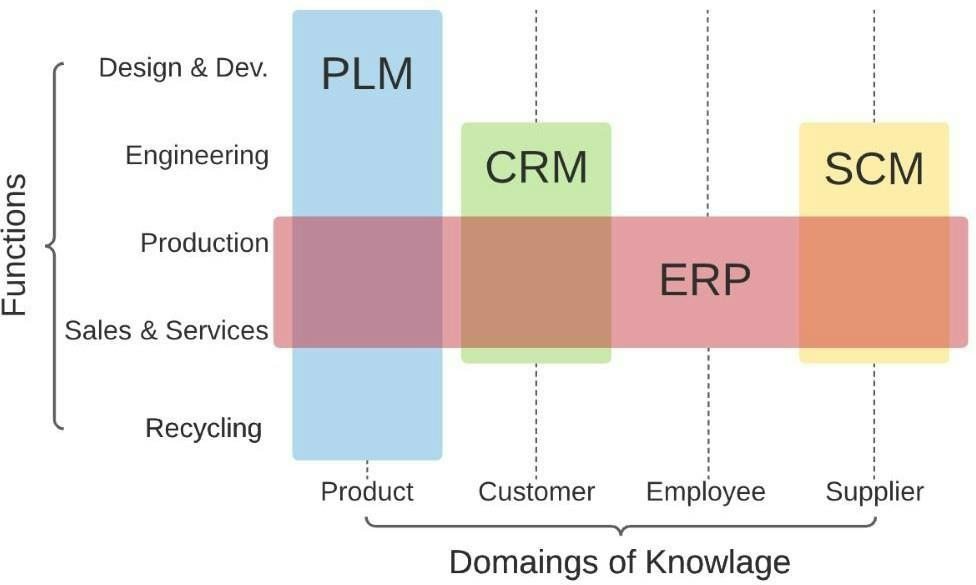
\includegraphics[width=418.64pt,height=250.05pt]{latexImage_27d831da3ed364aa5c6aec3df1a141ee.png}}
\put(87.38,-76.78003){\fontsize{14.04}{1}\usefont{T1}{ptm}{b}{n}\selectfont\color{color_29791}2}
\put(94.44212,-76.78003){\fontsize{14.04}{1}\usefont{T1}{ptm}{b}{n}\selectfont\color{color_29791}.2.}
\put(108.38,-76.78003){\fontsize{14.04}{1}\usefont{T1}{ptm}{b}{n}\selectfont\color{color_29791} }
\put(111.74,-76.78003){\fontsize{14.04}{1}\usefont{T1}{ptm}{b}{n}\selectfont\color{color_29791}企業資源規劃}
\put(195.17,-76.78003){\fontsize{14.04}{1}\usefont{T1}{ptm}{b}{n}\selectfont\color{color_29791} }
\put(82.944,-108.94){\fontsize{12}{1}\usefont{T1}{ptm}{m}{n}\selectfont\color{color_29791}在信息系統的早期}
\put(178.092,-108.94){\fontsize{12}{1}\usefont{T1}{ptm}{m}{n}\selectfont\color{color_29791},最}
\put(201.96,-108.94){\fontsize{12}{1}\usefont{T1}{ptm}{m}{n}\selectfont\color{color_29791}早得到廣泛實施的}
\put(297.108,-108.94){\fontsize{12}{1}\usefont{T1}{ptm}{m}{n}\selectfont\color{color_29791}系統}
\put(320.976,-108.94){\fontsize{12}{1}\usefont{T1}{ptm}{m}{n}\selectfont\color{color_29791}之一是稱為}
\put(380.47,-108.94){\fontsize{12}{1}\usefont{T1}{ptm}{m}{n}\selectfont\color{color_29791}M}
\put(391.03,-108.94){\fontsize{12}{1}\usefont{T1}{ptm}{m}{n}\selectfont\color{color_29791}R}
\put(398.95,-108.94){\fontsize{12}{1}\usefont{T1}{ptm}{m}{n}\selectfont\color{color_29791}P}
\put(405.55,-108.94){\fontsize{12}{1}\usefont{T1}{ptm}{m}{n}\selectfont\color{color_29791}(}
\put(417.43,-108.94){\fontsize{12}{1}\usefont{T1}{ptm}{m}{n}\selectfont\color{color_29791}物}
\put(429.31,-108.94){\fontsize{12}{1}\usefont{T1}{ptm}{m}{n}\selectfont\color{color_29791}料需}
\put(453.19,-108.94){\fontsize{12}{1}\usefont{T1}{ptm}{m}{n}\selectfont\color{color_29791}求}
\put(465.07,-108.94){\fontsize{12}{1}\usefont{T1}{ptm}{m}{n}\selectfont\color{color_29791}計}
\put(476.95,-108.94){\fontsize{12}{1}\usefont{T1}{ptm}{m}{n}\selectfont\color{color_29791}劃}
\put(488.83,-108.94){\fontsize{12}{1}\usefont{T1}{ptm}{m}{n}\selectfont\color{color_29791})}
\put(69.384,-126.82){\fontsize{12}{1}\usefont{T1}{ptm}{m}{n}\selectfont\color{color_29791}的系統。雖然不一}
\put(164.532,-126.82){\fontsize{12}{1}\usefont{T1}{ptm}{m}{n}\selectfont\color{color_29791}定是}
\put(188.4,-126.82){\fontsize{12}{1}\usefont{T1}{ptm}{m}{n}\selectfont\color{color_29791}基於軟體的,但這}
\put(283.548,-126.82){\fontsize{12}{1}\usefont{T1}{ptm}{m}{n}\selectfont\color{color_29791}種系}
\put(307.416,-126.82){\fontsize{12}{1}\usefont{T1}{ptm}{m}{n}\selectfont\color{color_29791}統範圍的實施是計}
\put(402.564,-126.82){\fontsize{12}{1}\usefont{T1}{ptm}{m}{n}\selectfont\color{color_29791}算技}
\put(426.432,-126.82){\fontsize{12}{1}\usefont{T1}{ptm}{m}{n}\selectfont\color{color_29791}術的自然結果}
\put(497.98,-126.82){\fontsize{12}{1}\usefont{T1}{ptm}{m}{n}\selectfont\color{color_29791} }
\put(69.384,-144.7){\fontsize{12}{1}\usefont{T1}{ptm}{m}{n}\selectfont\color{color_29791},它旨在通過計算}
\put(164.532,-144.7){\fontsize{12}{1}\usefont{T1}{ptm}{m}{n}\selectfont\color{color_29791}生產}
\put(188.4,-144.7){\fontsize{12}{1}\usefont{T1}{ptm}{m}{n}\selectfont\color{color_29791}的材料需求來解決}
\put(283.548,-144.7){\fontsize{12}{1}\usefont{T1}{ptm}{m}{n}\selectfont\color{color_29791}材料}
\put(307.416,-144.7){\fontsize{12}{1}\usefont{T1}{ptm}{m}{n}\selectfont\color{color_29791}供應和產品輸出方}
\put(402.564,-144.7){\fontsize{12}{1}\usefont{T1}{ptm}{m}{n}\selectfont\color{color_29791}面的}
\put(426.432,-144.7){\fontsize{12}{1}\usefont{T1}{ptm}{m}{n}\selectfont\color{color_29791}瓶頸。隨著它}
\put(497.86,-144.7){\fontsize{12}{1}\usefont{T1}{ptm}{m}{n}\selectfont\color{color_29791} }
\put(69.384,-162.58){\fontsize{12}{1}\usefont{T1}{ptm}{m}{n}\selectfont\color{color_29791}在}
\put(79.584,-162.58){\fontsize{12}{1}\usefont{T1}{ptm}{m}{n}\selectfont\color{color_29791} }
\put(83.784,-162.58){\fontsize{12}{1}\usefont{T1}{ptm}{m}{n}\selectfont\color{color_29791}70}
\put(95.78,-162.58){\fontsize{12}{1}\usefont{T1}{ptm}{m}{n}\selectfont\color{color_29791} }
\put(98.06,-162.58){\fontsize{12}{1}\usefont{T1}{ptm}{m}{n}\selectfont\color{color_29791}年代末和}
\put(143.18,-162.58){\fontsize{12}{1}\usefont{T1}{ptm}{m}{n}\selectfont\color{color_29791} }
\put(148.46,-162.58){\fontsize{12}{1}\usefont{T1}{ptm}{m}{n}\selectfont\color{color_29791}80}
\put(160.46,-162.58){\fontsize{12}{1}\usefont{T1}{ptm}{m}{n}\selectfont\color{color_29791} }
\put(162.74,-162.58){\fontsize{12}{1}\usefont{T1}{ptm}{m}{n}\selectfont\color{color_29791}年代}
\put(186.848,-162.58){\fontsize{12}{1}\usefont{T1}{ptm}{m}{n}\selectfont\color{color_29791}初在企業中變得越來越普遍,該系統不斷發展。這催生了}
\put(486.94,-162.58){\fontsize{12}{1}\usefont{T1}{ptm}{m}{n}\selectfont\color{color_29791}MR}
\put(505.648,-162.58){\fontsize{12}{1}\usefont{T1}{ptm}{m}{n}\selectfont\color{color_29791}P}
\put(512.356,-162.58){\fontsize{12}{1}\usefont{T1}{ptm}{m}{n}\selectfont\color{color_29791} }
\put(69.384,-180.58){\fontsize{12}{1}\usefont{T1}{ptm}{m}{n}\selectfont\color{color_29791}II}
\put(77.064,-180.58){\fontsize{12}{1}\usefont{T1}{ptm}{m}{n}\selectfont\color{color_29791}(}
\put(88.944,-180.58){\fontsize{12}{1}\usefont{T1}{ptm}{m}{n}\selectfont\color{color_29791}製}
\put(100.824,-180.58){\fontsize{12}{1}\usefont{T1}{ptm}{m}{n}\selectfont\color{color_29791}造資}
\put(124.704,-180.58){\fontsize{12}{1}\usefont{T1}{ptm}{m}{n}\selectfont\color{color_29791}源}
\put(136.584,-180.58){\fontsize{12}{1}\usefont{T1}{ptm}{m}{n}\selectfont\color{color_29791}規}
\put(148.464,-180.58){\fontsize{12}{1}\usefont{T1}{ptm}{m}{n}\selectfont\color{color_29791}劃}
\put(160.344,-180.58){\fontsize{12}{1}\usefont{T1}{ptm}{m}{n}\selectfont\color{color_29791}),對}
\put(196.224,-180.58){\fontsize{12}{1}\usefont{T1}{ptm}{m}{n}\selectfont\color{color_29791}本}
\put(208.104,-180.58){\fontsize{12}{1}\usefont{T1}{ptm}{m}{n}\selectfont\color{color_29791}文}
\put(219.984,-180.58){\fontsize{12}{1}\usefont{T1}{ptm}{m}{n}\selectfont\color{color_29791}的}
\put(231.864,-180.58){\fontsize{12}{1}\usefont{T1}{ptm}{m}{n}\selectfont\color{color_29791}範}
\put(243.744,-180.58){\fontsize{12}{1}\usefont{T1}{ptm}{m}{n}\selectfont\color{color_29791}圍}
\put(255.624,-180.58){\fontsize{12}{1}\usefont{T1}{ptm}{m}{n}\selectfont\color{color_29791}更}
\put(267.504,-180.58){\fontsize{12}{1}\usefont{T1}{ptm}{m}{n}\selectfont\color{color_29791}重要}
\put(291.384,-180.58){\fontsize{12}{1}\usefont{T1}{ptm}{m}{n}\selectfont\color{color_29791}的是}
\put(315.31,-180.58){\fontsize{12}{1}\usefont{T1}{ptm}{m}{n}\selectfont\color{color_29791}E}
\put(322.51,-180.58){\fontsize{12}{1}\usefont{T1}{ptm}{m}{n}\selectfont\color{color_29791}R}
\put(330.43,-180.58){\fontsize{12}{1}\usefont{T1}{ptm}{m}{n}\selectfont\color{color_29791}P}
\put(337.03,-180.58){\fontsize{12}{1}\usefont{T1}{ptm}{m}{n}\selectfont\color{color_29791}(}
\put(348.91,-180.58){\fontsize{12}{1}\usefont{T1}{ptm}{m}{n}\selectfont\color{color_29791}企}
\put(360.79,-180.58){\fontsize{12}{1}\usefont{T1}{ptm}{m}{n}\selectfont\color{color_29791}業}
\put(372.67,-180.58){\fontsize{12}{1}\usefont{T1}{ptm}{m}{n}\selectfont\color{color_29791}資}
\put(384.55,-180.58){\fontsize{12}{1}\usefont{T1}{ptm}{m}{n}\selectfont\color{color_29791}源}
\put(396.43,-180.58){\fontsize{12}{1}\usefont{T1}{ptm}{m}{n}\selectfont\color{color_29791}規}
\put(408.31,-180.58){\fontsize{12}{1}\usefont{T1}{ptm}{m}{n}\selectfont\color{color_29791}劃)}
\put(432.19,-180.58){\fontsize{12}{1}\usefont{T1}{ptm}{m}{n}\selectfont\color{color_29791}。}
\put(444.1,-180.58){\fontsize{12}{1}\usefont{T1}{ptm}{m}{n}\selectfont\color{color_29791} }
\put(63.024,-198.58){\fontsize{12}{1}\usefont{T1}{ptm}{m}{n}\selectfont\color{color_29791} }
\put(82.944,-214.06){\fontsize{12}{1}\usefont{T1}{ptm}{m}{n}\selectfont\color{color_29791}在大多數情況下,}
\put(178.092,-214.06){\fontsize{12}{1}\usefont{T1}{ptm}{m}{n}\selectfont\color{color_29791}現代}
\put(201.96,-214.06){\fontsize{12}{1}\usefont{T1}{ptm}{m}{n}\selectfont\color{color_29791}企業資源規劃擴展}
\put(297.108,-214.06){\fontsize{12}{1}\usefont{T1}{ptm}{m}{n}\selectfont\color{color_29791}了原}
\put(320.976,-214.06){\fontsize{12}{1}\usefont{T1}{ptm}{m}{n}\selectfont\color{color_29791}來}
\put(332.95,-214.06){\fontsize{12}{1}\usefont{T1}{ptm}{m}{n}\selectfont\color{color_29791}的}
\put(344.47,-214.06){\fontsize{12}{1}\usefont{T1}{ptm}{m}{n}\selectfont\color{color_29791} }
\put(487.66,-214.06){\fontsize{12}{1}\usefont{T1}{ptm}{m}{n}\selectfont\color{color_29791}M}
\put(498.1,-214.06){\fontsize{12}{1}\usefont{T1}{ptm}{m}{n}\selectfont\color{color_29791}R}
\put(505.9,-214.06){\fontsize{12}{1}\usefont{T1}{ptm}{m}{n}\selectfont\color{color_29791}P}
\put(512.26,-214.06){\fontsize{12}{1}\usefont{T1}{ptm}{m}{n}\selectfont\color{color_29791} }
\put(69.384,-232.06){\fontsize{12}{1}\usefont{T1}{ptm}{m}{n}\selectfont\color{color_29791}功}
\put(81.264,-232.06){\fontsize{12}{1}\usefont{T1}{ptm}{m}{n}\selectfont\color{color_29791}能}
\put(93.144,-232.06){\fontsize{12}{1}\usefont{T1}{ptm}{m}{n}\selectfont\color{color_29791},}
\put(105.024,-232.06){\fontsize{12}{1}\usefont{T1}{ptm}{m}{n}\selectfont\color{color_29791}以}
\put(116.904,-232.06){\fontsize{12}{1}\usefont{T1}{ptm}{m}{n}\selectfont\color{color_29791}涵}
\put(128.784,-232.06){\fontsize{12}{1}\usefont{T1}{ptm}{m}{n}\selectfont\color{color_29791}蓋}
\put(140.544,-232.06){\fontsize{12}{1}\usefont{T1}{ptm}{m}{n}\selectfont\color{color_29791}企}
\put(152.424,-232.06){\fontsize{12}{1}\usefont{T1}{ptm}{m}{n}\selectfont\color{color_29791}業}
\put(164.304,-232.06){\fontsize{12}{1}\usefont{T1}{ptm}{m}{n}\selectfont\color{color_29791}運}
\put(176.184,-232.06){\fontsize{12}{1}\usefont{T1}{ptm}{m}{n}\selectfont\color{color_29791}營}
\put(187.944,-232.06){\fontsize{12}{1}\usefont{T1}{ptm}{m}{n}\selectfont\color{color_29791}的}
\put(199.824,-232.06){\fontsize{12}{1}\usefont{T1}{ptm}{m}{n}\selectfont\color{color_29791}許}
\put(211.704,-232.06){\fontsize{12}{1}\usefont{T1}{ptm}{m}{n}\selectfont\color{color_29791}多}
\put(223.584,-232.06){\fontsize{12}{1}\usefont{T1}{ptm}{m}{n}\selectfont\color{color_29791}其}
\put(235.464,-232.06){\fontsize{12}{1}\usefont{T1}{ptm}{m}{n}\selectfont\color{color_29791}他}
\put(247.344,-232.06){\fontsize{12}{1}\usefont{T1}{ptm}{m}{n}\selectfont\color{color_29791}方}
\put(259.104,-232.06){\fontsize{12}{1}\usefont{T1}{ptm}{m}{n}\selectfont\color{color_29791}面}
\put(270.984,-232.06){\fontsize{12}{1}\usefont{T1}{ptm}{m}{n}\selectfont\color{color_29791},}
\put(282.864,-232.06){\fontsize{12}{1}\usefont{T1}{ptm}{m}{n}\selectfont\color{color_29791}同}
\put(294.744,-232.06){\fontsize{12}{1}\usefont{T1}{ptm}{m}{n}\selectfont\color{color_29791}時}
\put(306.5041,-232.06){\fontsize{12}{1}\usefont{T1}{ptm}{m}{n}\selectfont\color{color_29791}為}
\put(318.3841,-232.06){\fontsize{12}{1}\usefont{T1}{ptm}{m}{n}\selectfont\color{color_29791}系}
\put(330.2641,-232.06){\fontsize{12}{1}\usefont{T1}{ptm}{m}{n}\selectfont\color{color_29791}統}
\put(342.1441,-232.06){\fontsize{12}{1}\usefont{T1}{ptm}{m}{n}\selectfont\color{color_29791}增}
\put(354.0241,-232.06){\fontsize{12}{1}\usefont{T1}{ptm}{m}{n}\selectfont\color{color_29791}加}
\put(365.9041,-232.06){\fontsize{12}{1}\usefont{T1}{ptm}{m}{n}\selectfont\color{color_29791}了}
\put(377.6641,-232.06){\fontsize{12}{1}\usefont{T1}{ptm}{m}{n}\selectfont\color{color_29791}模}
\put(389.5441,-232.06){\fontsize{12}{1}\usefont{T1}{ptm}{m}{n}\selectfont\color{color_29791}組}
\put(401.4241,-232.06){\fontsize{12}{1}\usefont{T1}{ptm}{m}{n}\selectfont\color{color_29791}化}
\put(413.3041,-232.06){\fontsize{12}{1}\usefont{T1}{ptm}{m}{n}\selectfont\color{color_29791}。}
\put(425.11,-232.06){\fontsize{12}{1}\usefont{T1}{ptm}{m}{n}\selectfont\color{color_29791} }
\put(63.024,-251.29){\fontsize{12}{1}\usefont{T1}{ptm}{m}{n}\selectfont\color{color_29791} }
\put(82.944,-266.89){\fontsize{12}{1}\usefont{T1}{ptm}{m}{n}\selectfont\color{color_29791}現代}
\put(106.7,-266.89){\fontsize{12}{1}\usefont{T1}{ptm}{m}{n}\selectfont\color{color_29791}E}
\put(113.9,-266.89){\fontsize{12}{1}\usefont{T1}{ptm}{m}{n}\selectfont\color{color_29791}R}
\put(121.82,-266.89){\fontsize{12}{1}\usefont{T1}{ptm}{m}{n}\selectfont\color{color_29791}P}
\put(128.42,-266.89){\fontsize{12}{1}\usefont{T1}{ptm}{m}{n}\selectfont\color{color_29791}系}
\put(140.3,-266.89){\fontsize{12}{1}\usefont{T1}{ptm}{m}{n}\selectfont\color{color_29791}統}
\put(152.18,-266.89){\fontsize{12}{1}\usefont{T1}{ptm}{m}{n}\selectfont\color{color_29791}通}
\put(164.06,-266.89){\fontsize{12}{1}\usefont{T1}{ptm}{m}{n}\selectfont\color{color_29791}常}
\put(175.94,-266.89){\fontsize{12}{1}\usefont{T1}{ptm}{m}{n}\selectfont\color{color_29791}是}
\put(187.82,-266.89){\fontsize{12}{1}\usefont{T1}{ptm}{m}{n}\selectfont\color{color_29791}基於}
\put(211.7,-266.89){\fontsize{12}{1}\usefont{T1}{ptm}{m}{n}\selectfont\color{color_29791}模}
\put(223.58,-266.89){\fontsize{12}{1}\usefont{T1}{ptm}{m}{n}\selectfont\color{color_29791}組}
\put(235.46,-266.89){\fontsize{12}{1}\usefont{T1}{ptm}{m}{n}\selectfont\color{color_29791}的}
\put(247.37,-266.89){\fontsize{12}{1}\usefont{T1}{ptm}{m}{n}\selectfont\color{color_29791};}
\put(250.61,-266.89){\fontsize{12}{1}\usefont{T1}{ptm}{m}{n}\selectfont\color{color_29791}不}
\put(262.49,-266.89){\fontsize{12}{1}\usefont{T1}{ptm}{m}{n}\selectfont\color{color_29791}同}
\put(274.37,-266.89){\fontsize{12}{1}\usefont{T1}{ptm}{m}{n}\selectfont\color{color_29791}的}
\put(286.25,-266.89){\fontsize{12}{1}\usefont{T1}{ptm}{m}{n}\selectfont\color{color_29791}模組}
\put(310.13,-266.89){\fontsize{12}{1}\usefont{T1}{ptm}{m}{n}\selectfont\color{color_29791}具有}
\put(334.01,-266.89){\fontsize{12}{1}\usefont{T1}{ptm}{m}{n}\selectfont\color{color_29791}不}
\put(345.89,-266.89){\fontsize{12}{1}\usefont{T1}{ptm}{m}{n}\selectfont\color{color_29791}同}
\put(357.77,-266.89){\fontsize{12}{1}\usefont{T1}{ptm}{m}{n}\selectfont\color{color_29791}的}
\put(369.65,-266.89){\fontsize{12}{1}\usefont{T1}{ptm}{m}{n}\selectfont\color{color_29791}使}
\put(381.53,-266.89){\fontsize{12}{1}\usefont{T1}{ptm}{m}{n}\selectfont\color{color_29791}用}
\put(393.41,-266.89){\fontsize{12}{1}\usefont{T1}{ptm}{m}{n}\selectfont\color{color_29791}者}
\put(405.29,-266.89){\fontsize{12}{1}\usefont{T1}{ptm}{m}{n}\selectfont\color{color_29791}介面}
\put(429.17,-266.89){\fontsize{12}{1}\usefont{T1}{ptm}{m}{n}\selectfont\color{color_29791}和不}
\put(453.05,-266.89){\fontsize{12}{1}\usefont{T1}{ptm}{m}{n}\selectfont\color{color_29791}同}
\put(464.9301,-266.89){\fontsize{12}{1}\usefont{T1}{ptm}{m}{n}\selectfont\color{color_29791}的}
\put(476.8101,-266.89){\fontsize{12}{1}\usefont{T1}{ptm}{m}{n}\selectfont\color{color_29791}使}
\put(488.6901,-266.89){\fontsize{12}{1}\usefont{T1}{ptm}{m}{n}\selectfont\color{color_29791}用}
\put(69.384,-284.77){\fontsize{12}{1}\usefont{T1}{ptm}{m}{n}\selectfont\color{color_29791}者組。例如,製造}
\put(164.532,-284.77){\fontsize{12}{1}\usefont{T1}{ptm}{m}{n}\selectfont\color{color_29791}模組}
\put(188.4,-284.77){\fontsize{12}{1}\usefont{T1}{ptm}{m}{n}\selectfont\color{color_29791}、採購模組、物流}
\put(283.548,-284.77){\fontsize{12}{1}\usefont{T1}{ptm}{m}{n}\selectfont\color{color_29791}模組}
\put(307.416,-284.77){\fontsize{12}{1}\usefont{T1}{ptm}{m}{n}\selectfont\color{color_29791}、財務模組、維護}
\put(402.564,-284.77){\fontsize{12}{1}\usefont{T1}{ptm}{m}{n}\selectfont\color{color_29791}模組}
\put(426.432,-284.77){\fontsize{12}{1}\usefont{T1}{ptm}{m}{n}\selectfont\color{color_29791}、銷售模組。}
\put(497.98,-284.77){\fontsize{12}{1}\usefont{T1}{ptm}{m}{n}\selectfont\color{color_29791} }
\put(69.384,-302.65){\fontsize{12}{1}\usefont{T1}{ptm}{m}{n}\selectfont\color{color_29791}(}
\put(81.384,-302.65){\fontsize{12}{1}\usefont{T1}{ptm}{m}{n}\selectfont\color{color_29791}S}
\put(88.1,-302.65){\fontsize{12}{1}\usefont{T1}{ptm}{m}{n}\selectfont\color{color_29791}aa}
\put(98.66,-302.65){\fontsize{12}{1}\usefont{T1}{ptm}{m}{n}\selectfont\color{color_29791}ksvuori}
\put(134.66,-302.65){\fontsize{12}{1}\usefont{T1}{ptm}{m}{n}\selectfont\color{color_29791} }
\put(276.53,-302.65){\fontsize{12}{1}\usefont{T1}{ptm}{m}{n}\selectfont\color{color_29791}和}
\put(288.53,-302.65){\fontsize{12}{1}\usefont{T1}{ptm}{m}{n}\selectfont\color{color_29791} }
\put(430.39,-302.65){\fontsize{12}{1}\usefont{T1}{ptm}{m}{n}\selectfont\color{color_29791}I}
\put(433.99,-302.65){\fontsize{12}{1}\usefont{T1}{ptm}{m}{n}\selectfont\color{color_29791}m}
\put(443.23,-302.65){\fontsize{12}{1}\usefont{T1}{ptm}{m}{n}\selectfont\color{color_29791}m}
\put(452.47,-302.65){\fontsize{12}{1}\usefont{T1}{ptm}{m}{n}\selectfont\color{color_29791}o}
\put(458.35,-302.65){\fontsize{12}{1}\usefont{T1}{ptm}{m}{n}\selectfont\color{color_29791}n}
\put(464.26,-302.65){\fontsize{12}{1}\usefont{T1}{ptm}{m}{n}\selectfont\color{color_29791}e}
\put(469.42,-302.65){\fontsize{12}{1}\usefont{T1}{ptm}{m}{n}\selectfont\color{color_29791}n}
\put(475.42,-302.65){\fontsize{12}{1}\usefont{T1}{ptm}{m}{n}\selectfont\color{color_29791},}
\put(487.3,-302.65){\fontsize{12}{1}\usefont{T1}{ptm}{m}{n}\selectfont\color{color_29791}20}
\put(499.06,-302.65){\fontsize{12}{1}\usefont{T1}{ptm}{m}{n}\selectfont\color{color_29791}0}
\put(505.06,-302.65){\fontsize{12}{1}\usefont{T1}{ptm}{m}{n}\selectfont\color{color_29791}8}
\put(69.384,-320.53){\fontsize{12}{1}\usefont{T1}{ptm}{m}{n}\selectfont\color{color_29791}年)}
\put(93.38,-320.53){\fontsize{12}{1}\usefont{T1}{ptm}{m}{n}\selectfont\color{color_29791}。}
\put(105.38,-320.53){\fontsize{12}{1}\usefont{T1}{ptm}{m}{n}\selectfont\color{color_29791}這些模組擴展到許多知識領域,但在大多數情況下,它們總是從生產、銷售}
\put(69.384,-338.41){\fontsize{12}{1}\usefont{T1}{ptm}{m}{n}\selectfont\color{color_29791}和服務的角度出}
\put(153.38,-338.41){\fontsize{12}{1}\usefont{T1}{ptm}{m}{n}\selectfont\color{color_29791}發}
\put(165.38,-338.41){\fontsize{12}{1}\usefont{T1}{ptm}{m}{n}\selectfont\color{color_29791}。圖}
\put(189.41,-338.41){\fontsize{12}{1}\usefont{T1}{ptm}{m}{n}\selectfont\color{color_29791}2}
\put(195.41,-338.41){\fontsize{12}{1}\usefont{T1}{ptm}{m}{n}\selectfont\color{color_29791}描述了}
\put(231.41,-338.41){\fontsize{12}{1}\usefont{T1}{ptm}{m}{n}\selectfont\color{color_29791}ER}
\put(246.77,-338.41){\fontsize{12}{1}\usefont{T1}{ptm}{m}{n}\selectfont\color{color_29791}P}
\put(253.49,-338.41){\fontsize{12}{1}\usefont{T1}{ptm}{m}{n}\selectfont\color{color_29791}系統與}
\put(289.49,-338.41){\fontsize{12}{1}\usefont{T1}{ptm}{m}{n}\selectfont\color{color_29791}其}
\put(301.25,-338.41){\fontsize{12}{1}\usefont{T1}{ptm}{m}{n}\selectfont\color{color_29791}他資訊系統的比較範圍。}
\put(433.27,-338.41){\fontsize{12}{1}\usefont{T1}{ptm}{m}{n}\selectfont\color{color_29791} }
\put(63.024,-354.25){\fontsize{9.96}{1}\usefont{T1}{ptm}{m}{n}\selectfont\color{color_29791} }
\put(63.024,-367.21){\fontsize{9.96}{1}\usefont{T1}{ptm}{m}{n}\selectfont\color{color_29791} }
\put(63.024,-384.97){\fontsize{9.96}{1}\usefont{T1}{ptm}{m}{n}\selectfont\color{color_29791} }
\put(138.86,-654.42){\fontsize{12}{1}\usefont{T1}{ptm}{b}{n}\selectfont\color{color_29791}圖}
\put(150.86,-654.42){\fontsize{12}{1}\usefont{T1}{ptm}{b}{n}\selectfont\color{color_29791}2}
\put(156.86,-654.42){\fontsize{12}{1}\usefont{T1}{ptm}{b}{n}\selectfont\color{color_29791} }
\put(159.86,-654.42){\fontsize{12}{1}\usefont{T1}{ptm}{b}{n}\selectfont\color{color_29791}不同資訊系統範圍的視覺化表示(改編自}
\put(375.91,-654.42){\fontsize{12}{1}\usefont{T1}{ptm}{b}{n}\selectfont\color{color_29791}S}
\put(382.618,-654.42){\fontsize{12}{1}\usefont{T1}{ptm}{b}{n}\selectfont\color{color_29791}tar}
\put(397.858,-654.42){\fontsize{12}{1}\usefont{T1}{ptm}{b}{n}\selectfont\color{color_29791}k}
\put(404.59,-654.42){\fontsize{12}{1}\usefont{T1}{ptm}{b}{n}\selectfont\color{color_29791} }
\put(407.83,-654.42){\fontsize{12}{1}\usefont{T1}{ptm}{b}{n}\selectfont\color{color_29791}2015}
\put(431.35,-654.42){\fontsize{12}{1}\usefont{T1}{ptm}{b}{n}\selectfont\color{color_29791})}
\put(443.26,-654.42){\fontsize{12}{1}\usefont{T1}{ptm}{b}{n}\selectfont\color{color_29791} }
\end{picture}
\newpage
\begin{tikzpicture}[overlay]\path(0pt,0pt);\end{tikzpicture}
\begin{picture}(-5,0)(2.5,0)
\put(500.26,-727.616){\fontsize{12}{1}\usefont{T1}{ptm}{m}{n}\selectfont\color{color_29791}7}
\put(506.02,-727.616){\fontsize{12}{1}\usefont{T1}{ptm}{m}{n}\selectfont\color{color_29791} }
\put(63.024,-726.896){\fontsize{9.96}{1}\usefont{T1}{ptm}{m}{n}\selectfont\color{color_29791} }
\put(168.45,-437.2){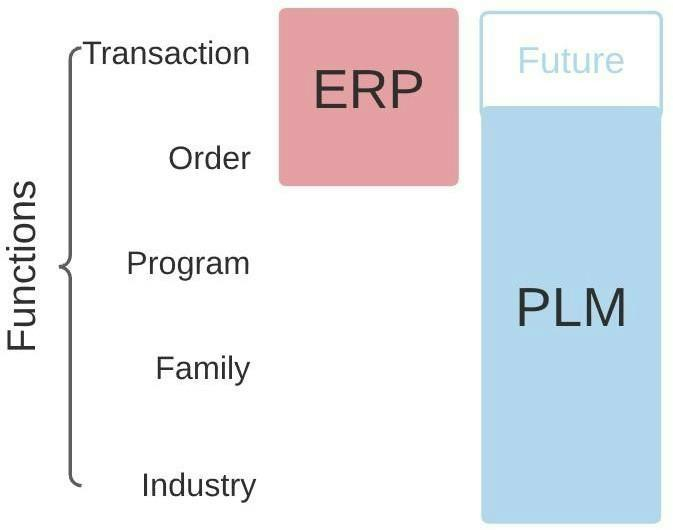
\includegraphics[width=252.35pt,height=198.75pt]{latexImage_67807e61aedd53f708ba7080fc4eb3d4.png}}
\put(82.944,-72.56){\fontsize{12}{1}\usefont{T1}{ptm}{m}{n}\selectfont\color{color_29791}這種跨域的廣泛覆蓋是有道理的,因為}
\put(286.97,-72.56){\fontsize{15}{1}\usefont{T1}{ptm}{m}{n}\selectfont\color{color_29791} }
\put(299.912,-72.56){\fontsize{15}{1}\usefont{T1}{ptm}{m}{n}\selectfont\color{color_29791} }
\put(312.98,-72.56){\fontsize{15}{1}\usefont{T1}{ptm}{m}{n}\selectfont\color{color_29791} }
\put(325.99,-72.56){\fontsize{12}{1}\usefont{T1}{ptm}{m}{n}\selectfont\color{color_29791}ERP}
\put(348.07,-72.56){\fontsize{12}{1}\usefont{T1}{ptm}{m}{n}\selectfont\color{color_29791} }
\put(403.87,-72.56){\fontsize{12}{1}\usefont{T1}{ptm}{m}{n}\selectfont\color{color_29791}操作與}
\put(444.34,-72.56){\fontsize{15}{1}\usefont{T1}{ptm}{m}{n}\selectfont\color{color_29791} }
\put(458.722,-72.56){\fontsize{15}{1}\usefont{T1}{ptm}{m}{n}\selectfont\color{color_29791} }
\put(473.23,-72.56){\fontsize{15}{1}\usefont{T1}{ptm}{m}{n}\selectfont\color{color_29791} }
\put(487.66,-72.56){\fontsize{12}{1}\usefont{T1}{ptm}{m}{n}\selectfont\color{color_29791}MR}
\put(506.368,-72.56){\fontsize{12}{1}\usefont{T1}{ptm}{m}{n}\selectfont\color{color_29791}P}
\put(69.384,-90.34003){\fontsize{12}{1}\usefont{T1}{ptm}{m}{n}\selectfont\color{color_29791}一樣,}
\put(105.492,-90.34003){\fontsize{12}{1}\usefont{T1}{ptm}{m}{n}\selectfont\color{color_29791}專注}
\put(129.6,-90.34003){\fontsize{12}{1}\usefont{T1}{ptm}{m}{n}\selectfont\color{color_29791}於處}
\put(153.708,-90.34003){\fontsize{12}{1}\usefont{T1}{ptm}{m}{n}\selectfont\color{color_29791}理交}
\put(177.816,-90.34003){\fontsize{12}{1}\usefont{T1}{ptm}{m}{n}\selectfont\color{color_29791}易}
\put(189.924,-90.34003){\fontsize{12}{1}\usefont{T1}{ptm}{m}{n}\selectfont\color{color_29791}和訂單}
\put(226.032,-90.34003){\fontsize{12}{1}\usefont{T1}{ptm}{m}{n}\selectfont\color{color_29791}。}
\put(238.13,-90.34003){\fontsize{12}{1}\usefont{T1}{ptm}{m}{n}\selectfont\color{color_29791}E}
\put(245.33,-90.34003){\fontsize{12}{1}\usefont{T1}{ptm}{m}{n}\selectfont\color{color_29791}R}
\put(253.25,-90.34003){\fontsize{12}{1}\usefont{T1}{ptm}{m}{n}\selectfont\color{color_29791}P}
\put(260.09,-90.34003){\fontsize{12}{1}\usefont{T1}{ptm}{m}{n}\selectfont\color{color_29791}的重}
\put(284.198,-90.34003){\fontsize{12}{1}\usefont{T1}{ptm}{m}{n}\selectfont\color{color_29791}點是}
\put(308.306,-90.34003){\fontsize{12}{1}\usefont{T1}{ptm}{m}{n}\selectfont\color{color_29791}控制公}
\put(344.414,-90.34003){\fontsize{12}{1}\usefont{T1}{ptm}{m}{n}\selectfont\color{color_29791}司資}
\put(368.522,-90.34003){\fontsize{12}{1}\usefont{T1}{ptm}{m}{n}\selectfont\color{color_29791}源的}
\put(392.63,-90.34003){\fontsize{12}{1}\usefont{T1}{ptm}{m}{n}\selectfont\color{color_29791}輸入}
\put(416.738,-90.34003){\fontsize{12}{1}\usefont{T1}{ptm}{m}{n}\selectfont\color{color_29791}、}
\put(428.846,-90.34003){\fontsize{12}{1}\usefont{T1}{ptm}{m}{n}\selectfont\color{color_29791}保留和}
\put(464.954,-90.34003){\fontsize{12}{1}\usefont{T1}{ptm}{m}{n}\selectfont\color{color_29791}輸出}
\put(489.062,-90.34003){\fontsize{12}{1}\usefont{T1}{ptm}{m}{n}\selectfont\color{color_29791}的變}
\put(69.384,-108.34){\fontsize{12}{1}\usefont{T1}{ptm}{m}{n}\selectfont\color{color_29791}化,無論是產品、}
\put(164.532,-108.34){\fontsize{12}{1}\usefont{T1}{ptm}{m}{n}\selectfont\color{color_29791}原材}
\put(188.4,-108.34){\fontsize{12}{1}\usefont{T1}{ptm}{m}{n}\selectfont\color{color_29791}料還是包裝。}
\put(259.85,-108.34){\fontsize{12}{1}\usefont{T1}{ptm}{m}{n}\selectfont\color{color_29791} }
\put(63.024,-126.46){\fontsize{12}{1}\usefont{T1}{ptm}{m}{n}\selectfont\color{color_29791} }
\put(82.944,-142.06){\fontsize{12}{1}\usefont{T1}{ptm}{m}{n}\selectfont\color{color_29791}從同一張圖片}
\put(154.94,-142.06){\fontsize{12}{1}\usefont{T1}{ptm}{m}{n}\selectfont\color{color_29791}中}
\put(166.94,-142.06){\fontsize{12}{1}\usefont{T1}{ptm}{m}{n}\selectfont\color{color_29791},可以看出}
\put(226.97,-142.06){\fontsize{12}{1}\usefont{T1}{ptm}{m}{n}\selectfont\color{color_29791}P}
\put(233.81,-142.06){\fontsize{12}{1}\usefont{T1}{ptm}{m}{n}\selectfont\color{color_29791}L}
\put(240.89,-142.06){\fontsize{12}{1}\usefont{T1}{ptm}{m}{n}\selectfont\color{color_29791}M}
\put(251.57,-142.06){\fontsize{12}{1}\usefont{T1}{ptm}{m}{n}\selectfont\color{color_29791}和}
\put(263.57,-142.06){\fontsize{12}{1}\usefont{T1}{ptm}{m}{n}\selectfont\color{color_29791}ER}
\put(278.93,-142.06){\fontsize{12}{1}\usefont{T1}{ptm}{m}{n}\selectfont\color{color_29791}P}
\put(285.65,-142.06){\fontsize{12}{1}\usefont{T1}{ptm}{m}{n}\selectfont\color{color_29791}之間的}
\put(321.53,-142.06){\fontsize{12}{1}\usefont{T1}{ptm}{m}{n}\selectfont\color{color_29791}理論對比,儘管它們都非常廣泛。}
\put(501.58,-142.06){\fontsize{12}{1}\usefont{T1}{ptm}{m}{n}\selectfont\color{color_29791}E }
\put(69.384,-159.94){\fontsize{12}{1}\usefont{T1}{ptm}{m}{n}\selectfont\color{color_29791}RP}
\put(84.144,-159.94){\fontsize{12}{1}\usefont{T1}{ptm}{m}{n}\selectfont\color{color_29791}擴展到知識領}
\put(156.14,-159.94){\fontsize{12}{1}\usefont{T1}{ptm}{m}{n}\selectfont\color{color_29791}域}
\put(168.14,-159.94){\fontsize{12}{1}\usefont{T1}{ptm}{m}{n}\selectfont\color{color_29791},}
\put(180.17,-159.94){\fontsize{12}{1}\usefont{T1}{ptm}{m}{n}\selectfont\color{color_29791}但}
\put(191.93,-159.94){\fontsize{12}{1}\usefont{T1}{ptm}{m}{n}\selectfont\color{color_29791}僅限於少數功能,而}
\put(299.93,-159.94){\fontsize{12}{1}\usefont{T1}{ptm}{m}{n}\selectfont\color{color_29791}P}
\put(306.77,-159.94){\fontsize{12}{1}\usefont{T1}{ptm}{m}{n}\selectfont\color{color_29791}L}
\put(313.99,-159.94){\fontsize{12}{1}\usefont{T1}{ptm}{m}{n}\selectfont\color{color_29791}M}
\put(324.67,-159.94){\fontsize{12}{1}\usefont{T1}{ptm}{m}{n}\selectfont\color{color_29791}則擴展到涉及產品的所有功能。如}
\put(69.384,-177.82){\fontsize{12}{1}\usefont{T1}{ptm}{m}{n}\selectfont\color{color_29791}圖}
\put(81.384,-177.82){\fontsize{12}{1}\usefont{T1}{ptm}{m}{n}\selectfont\color{color_29791} }
\put(101.9,-177.82){\fontsize{12}{1}\usefont{T1}{ptm}{m}{n}\selectfont\color{color_29791}3}
\put(107.9,-177.82){\fontsize{12}{1}\usefont{T1}{ptm}{m}{n}\selectfont\color{color_29791} }
\put(128.42,-177.82){\fontsize{12}{1}\usefont{T1}{ptm}{m}{n}\selectfont\color{color_29791}所示,代}
\put(176.42,-177.82){\fontsize{12}{1}\usefont{T1}{ptm}{m}{n}\selectfont\color{color_29791}表}
\put(188.57,-177.82){\fontsize{12}{1}\usefont{T1}{ptm}{m}{n}\selectfont\color{color_29791}兩者之間良好差異的另一個觀點}
\put(356.59,-177.82){\fontsize{12}{1}\usefont{T1}{ptm}{m}{n}\selectfont\color{color_29791}是}
\put(368.59,-177.82){\fontsize{12}{1}\usefont{T1}{ptm}{m}{n}\selectfont\color{color_29791},在}
\put(392.59,-177.82){\fontsize{12}{1}\usefont{T1}{ptm}{m}{n}\selectfont\color{color_29791} }
\put(413.23,-177.82){\fontsize{12}{1}\usefont{T1}{ptm}{m}{n}\selectfont\color{color_29791}ER}
\put(428.59,-177.82){\fontsize{12}{1}\usefont{T1}{ptm}{m}{n}\selectfont\color{color_29791}P}
\put(435.19,-177.82){\fontsize{12}{1}\usefont{T1}{ptm}{m}{n}\selectfont\color{color_29791} }
\put(455.38,-177.82){\fontsize{12}{1}\usefont{T1}{ptm}{m}{n}\selectfont\color{color_29791}和}
\put(467.38,-177.82){\fontsize{12}{1}\usefont{T1}{ptm}{m}{n}\selectfont\color{color_29791} }
\put(487.9,-177.82){\fontsize{12}{1}\usefont{T1}{ptm}{m}{n}\selectfont\color{color_29791}P}
\put(494.5,-177.82){\fontsize{12}{1}\usefont{T1}{ptm}{m}{n}\selectfont\color{color_29791}L}
\put(501.22,-177.82){\fontsize{12}{1}\usefont{T1}{ptm}{m}{n}\selectfont\color{color_29791}M}
\put(69.384,-195.7){\fontsize{12}{1}\usefont{T1}{ptm}{m}{n}\selectfont\color{color_29791}影響行業的規模或詳細程度(即兩個系統的粒度)方面缺乏重疊。}
\put(417.43,-195.7){\fontsize{12}{1}\usefont{T1}{ptm}{m}{n}\selectfont\color{color_29791} }
\put(63.024,-211.54){\fontsize{9.96}{1}\usefont{T1}{ptm}{m}{n}\selectfont\color{color_29791} }
\put(63.024,-234.58){\fontsize{9.96}{1}\usefont{T1}{ptm}{m}{n}\selectfont\color{color_29791} }
\put(122.78,-456.27){\fontsize{12}{1}\usefont{T1}{ptm}{b}{n}\selectfont\color{color_29791}圖}
\put(134.78,-456.27){\fontsize{12}{1}\usefont{T1}{ptm}{b}{n}\selectfont\color{color_29791}3}
\put(140.78,-456.27){\fontsize{12}{1}\usefont{T1}{ptm}{b}{n}\selectfont\color{color_29791} }
\put(143.78,-456.27){\fontsize{12}{1}\usefont{T1}{ptm}{b}{n}\selectfont\color{color_29791}E}
\put(151.808,-456.27){\fontsize{12}{1}\usefont{T1}{ptm}{b}{n}\selectfont\color{color_29791}RP}
\put(167.78,-456.27){\fontsize{12}{1}\usefont{T1}{ptm}{b}{n}\selectfont\color{color_29791}和}
\put(179.81,-456.27){\fontsize{12}{1}\usefont{T1}{ptm}{b}{n}\selectfont\color{color_29791}PLM}
\put(206.45,-456.27){\fontsize{12}{1}\usefont{T1}{ptm}{b}{n}\selectfont\color{color_29791}在粒度}
\put(242.558,-456.27){\fontsize{12}{1}\usefont{T1}{ptm}{b}{n}\selectfont\color{color_29791}方面的可視化比較(改編自}
\put(386.59,-456.27){\fontsize{12}{1}\usefont{T1}{ptm}{b}{n}\selectfont\color{color_29791}S}
\put(393.19,-456.27){\fontsize{12}{1}\usefont{T1}{ptm}{b}{n}\selectfont\color{color_29791}t}
\put(397.03,-456.27){\fontsize{12}{1}\usefont{T1}{ptm}{b}{n}\selectfont\color{color_29791}a}
\put(402.91,-456.27){\fontsize{12}{1}\usefont{T1}{ptm}{b}{n}\selectfont\color{color_29791}r}
\put(408.07,-456.27){\fontsize{12}{1}\usefont{T1}{ptm}{b}{n}\selectfont\color{color_29791}k}
\put(414.67,-456.27){\fontsize{12}{1}\usefont{T1}{ptm}{b}{n}\selectfont\color{color_29791},}
\put(426.55,-456.27){\fontsize{12}{1}\usefont{T1}{ptm}{b}{n}\selectfont\color{color_29791}2}
\put(432.43,-456.27){\fontsize{12}{1}\usefont{T1}{ptm}{b}{n}\selectfont\color{color_29791}0}
\put(438.31,-456.27){\fontsize{12}{1}\usefont{T1}{ptm}{b}{n}\selectfont\color{color_29791}15}
\put(450.22,-456.27){\fontsize{12}{1}\usefont{T1}{ptm}{b}{n}\selectfont\color{color_29791})}
\put(462.22,-456.27){\fontsize{12}{1}\usefont{T1}{ptm}{b}{n}\selectfont\color{color_29791} }
\put(82.944,-489.75){\fontsize{12}{1}\usefont{T1}{ptm}{m}{n}\selectfont\color{color_29791}正如我}
\put(118.824,-489.75){\fontsize{12}{1}\usefont{T1}{ptm}{m}{n}\selectfont\color{color_29791}們所看}
\put(154.704,-489.75){\fontsize{12}{1}\usefont{T1}{ptm}{m}{n}\selectfont\color{color_29791}到的}
\put(178.584,-489.75){\fontsize{12}{1}\usefont{T1}{ptm}{m}{n}\selectfont\color{color_29791},}
\put(190.61,-489.75){\fontsize{12}{1}\usefont{T1}{ptm}{m}{n}\selectfont\color{color_29791}ER}
\put(205.73,-489.75){\fontsize{12}{1}\usefont{T1}{ptm}{m}{n}\selectfont\color{color_29791}P}
\put(212.45,-489.75){\fontsize{12}{1}\usefont{T1}{ptm}{m}{n}\selectfont\color{color_29791}主要關}
\put(248.33,-489.75){\fontsize{12}{1}\usefont{T1}{ptm}{m}{n}\selectfont\color{color_29791}注交易}
\put(284.21,-489.75){\fontsize{12}{1}\usefont{T1}{ptm}{m}{n}\selectfont\color{color_29791}和訂}
\put(308.09,-489.75){\fontsize{12}{1}\usefont{T1}{ptm}{m}{n}\selectfont\color{color_29791}單}
\put(319.97,-489.75){\fontsize{12}{1}\usefont{T1}{ptm}{m}{n}\selectfont\color{color_29791}。一旦}
\put(355.85,-489.75){\fontsize{12}{1}\usefont{T1}{ptm}{m}{n}\selectfont\color{color_29791}訂單被}
\put(391.73,-489.75){\fontsize{12}{1}\usefont{T1}{ptm}{m}{n}\selectfont\color{color_29791}關閉}
\put(415.61,-489.75){\fontsize{12}{1}\usefont{T1}{ptm}{m}{n}\selectfont\color{color_29791},}
\put(427.63,-489.75){\fontsize{12}{1}\usefont{T1}{ptm}{m}{n}\selectfont\color{color_29791}ER}
\put(442.78,-489.75){\fontsize{12}{1}\usefont{T1}{ptm}{m}{n}\selectfont\color{color_29791}P}
\put(449.62,-489.75){\fontsize{12}{1}\usefont{T1}{ptm}{m}{n}\selectfont\color{color_29791}系}
\put(461.5,-489.75){\fontsize{12}{1}\usefont{T1}{ptm}{m}{n}\selectfont\color{color_29791}統}
\put(473.38,-489.75){\fontsize{12}{1}\usefont{T1}{ptm}{m}{n}\selectfont\color{color_29791}就}
\put(485.14,-489.75){\fontsize{12}{1}\usefont{T1}{ptm}{m}{n}\selectfont\color{color_29791}會}
\put(497.02,-489.75){\fontsize{12}{1}\usefont{T1}{ptm}{m}{n}\selectfont\color{color_29791}處}
\put(69.384,-507.75){\fontsize{12}{1}\usefont{T1}{ptm}{m}{n}\selectfont\color{color_29791}理與該訂單相關的交易,但不太關心超出該訂單的訂單。另一方面,}
\put(429.43,-507.75){\fontsize{12}{1}\usefont{T1}{ptm}{m}{n}\selectfont\color{color_29791}P}
\put(436.27,-507.75){\fontsize{12}{1}\usefont{T1}{ptm}{m}{n}\selectfont\color{color_29791}L}
\put(443.38,-507.75){\fontsize{12}{1}\usefont{T1}{ptm}{m}{n}\selectfont\color{color_29791}M}
\put(454.06,-507.75){\fontsize{12}{1}\usefont{T1}{ptm}{m}{n}\selectfont\color{color_29791}的粒度與}
\put(69.384,-525.63){\fontsize{12}{1}\usefont{T1}{ptm}{m}{n}\selectfont\color{color_29791}產品的}
\put(105.264,-525.63){\fontsize{12}{1}\usefont{T1}{ptm}{m}{n}\selectfont\color{color_29791}訂單有}
\put(141.144,-525.63){\fontsize{12}{1}\usefont{T1}{ptm}{m}{n}\selectfont\color{color_29791}關,}
\put(165.024,-525.63){\fontsize{12}{1}\usefont{T1}{ptm}{m}{n}\selectfont\color{color_29791}不僅}
\put(188.904,-525.63){\fontsize{12}{1}\usefont{T1}{ptm}{m}{n}\selectfont\color{color_29791}延伸到}
\put(224.784,-525.63){\fontsize{12}{1}\usefont{T1}{ptm}{m}{n}\selectfont\color{color_29791}程式中}
\put(260.664,-525.63){\fontsize{12}{1}\usefont{T1}{ptm}{m}{n}\selectfont\color{color_29791},還}
\put(284.544,-525.63){\fontsize{12}{1}\usefont{T1}{ptm}{m}{n}\selectfont\color{color_29791}延伸}
\put(308.424,-525.63){\fontsize{12}{1}\usefont{T1}{ptm}{m}{n}\selectfont\color{color_29791}到家庭}
\put(344.304,-525.63){\fontsize{12}{1}\usefont{T1}{ptm}{m}{n}\selectfont\color{color_29791}和整個}
\put(380.1841,-525.63){\fontsize{12}{1}\usefont{T1}{ptm}{m}{n}\selectfont\color{color_29791}行業}
\put(404.23,-525.63){\fontsize{12}{1}\usefont{T1}{ptm}{m}{n}\selectfont\color{color_29791}(}
\put(416.11,-525.63){\fontsize{12}{1}\usefont{T1}{ptm}{m}{n}\selectfont\color{color_29791}S}
\put(422.83,-525.63){\fontsize{12}{1}\usefont{T1}{ptm}{m}{n}\selectfont\color{color_29791}t}
\put(426.07,-525.63){\fontsize{12}{1}\usefont{T1}{ptm}{m}{n}\selectfont\color{color_29791}a}
\put(431.23,-525.63){\fontsize{12}{1}\usefont{T1}{ptm}{m}{n}\selectfont\color{color_29791}r}
\put(435.19,-525.63){\fontsize{12}{1}\usefont{T1}{ptm}{m}{n}\selectfont\color{color_29791}k}
\put(441.22,-525.63){\fontsize{12}{1}\usefont{T1}{ptm}{m}{n}\selectfont\color{color_29791},}
\put(453.22,-525.63){\fontsize{12}{1}\usefont{T1}{ptm}{m}{n}\selectfont\color{color_29791}2015}
\put(477.22,-525.63){\fontsize{12}{1}\usefont{T1}{ptm}{m}{n}\selectfont\color{color_29791})。}
\put(501.22,-525.63){\fontsize{12}{1}\usefont{T1}{ptm}{m}{n}\selectfont\color{color_29791} }
\put(63.024,-543.87){\fontsize{12}{1}\usefont{T1}{ptm}{m}{n}\selectfont\color{color_29791} }
\put(82.944,-559.59){\fontsize{12}{1}\usefont{T1}{ptm}{m}{n}\selectfont\color{color_29791}這特別有趣,因為}
\put(178.092,-559.59){\fontsize{12}{1}\usefont{T1}{ptm}{m}{n}\selectfont\color{color_29791}它展}
\put(201.96,-559.59){\fontsize{12}{1}\usefont{T1}{ptm}{m}{n}\selectfont\color{color_29791}示了這兩個系統如}
\put(297.108,-559.59){\fontsize{12}{1}\usefont{T1}{ptm}{m}{n}\selectfont\color{color_29791}何能}
\put(320.976,-559.59){\fontsize{12}{1}\usefont{T1}{ptm}{m}{n}\selectfont\color{color_29791}夠並且確實在現場}
\put(416.124,-559.59){\fontsize{12}{1}\usefont{T1}{ptm}{m}{n}\selectfont\color{color_29791}相互}
\put(439.992,-559.59){\fontsize{12}{1}\usefont{T1}{ptm}{m}{n}\selectfont\color{color_29791}補充。}
\put(475.78,-559.59){\fontsize{12}{1}\usefont{T1}{ptm}{m}{n}\selectfont\color{color_29791}E}
\put(482.98,-559.59){\fontsize{12}{1}\usefont{T1}{ptm}{m}{n}\selectfont\color{color_29791}R}
\put(490.9,-559.59){\fontsize{12}{1}\usefont{T1}{ptm}{m}{n}\selectfont\color{color_29791}P}
\put(69.384,-577.5){\fontsize{12}{1}\usefont{T1}{ptm}{m}{n}\selectfont\color{color_29791}應該指出的一個方}
\put(164.532,-577.5){\fontsize{12}{1}\usefont{T1}{ptm}{m}{n}\selectfont\color{color_29791}面是}
\put(188.4,-577.5){\fontsize{12}{1}\usefont{T1}{ptm}{m}{n}\selectfont\color{color_29791},它與其他系統集}
\put(283.548,-577.5){\fontsize{12}{1}\usefont{T1}{ptm}{m}{n}\selectfont\color{color_29791}成相}
\put(307.416,-577.5){\fontsize{12}{1}\usefont{T1}{ptm}{m}{n}\selectfont\color{color_29791}對容易。例如,}
\put(390.67,-577.5){\fontsize{12}{1}\usefont{T1}{ptm}{m}{n}\selectfont\color{color_29791}E}
\put(397.87,-577.5){\fontsize{12}{1}\usefont{T1}{ptm}{m}{n}\selectfont\color{color_29791}R}
\put(405.79,-577.5){\fontsize{12}{1}\usefont{T1}{ptm}{m}{n}\selectfont\color{color_29791}P}
\put(412.51,-577.5){\fontsize{12}{1}\usefont{T1}{ptm}{m}{n}\selectfont\color{color_29791}-}
\put(416.47,-577.5){\fontsize{12}{1}\usefont{T1}{ptm}{m}{n}\selectfont\color{color_29791} }
\put(69.384,-595.38){\fontsize{12}{1}\usefont{T1}{ptm}{m}{n}\selectfont\color{color_29791}M}
\put(79.944,-595.38){\fontsize{12}{1}\usefont{T1}{ptm}{m}{n}\selectfont\color{color_29791}E}
\put(87.144,-595.38){\fontsize{12}{1}\usefont{T1}{ptm}{m}{n}\selectfont\color{color_29791}S}
\put(93.74,-595.38){\fontsize{12}{1}\usefont{T1}{ptm}{m}{n}\selectfont\color{color_29791}集}
\put(105.62,-595.38){\fontsize{12}{1}\usefont{T1}{ptm}{m}{n}\selectfont\color{color_29791}成}
\put(117.5,-595.38){\fontsize{12}{1}\usefont{T1}{ptm}{m}{n}\selectfont\color{color_29791}已}
\put(129.38,-595.38){\fontsize{12}{1}\usefont{T1}{ptm}{m}{n}\selectfont\color{color_29791}被}
\put(141.26,-595.38){\fontsize{12}{1}\usefont{T1}{ptm}{m}{n}\selectfont\color{color_29791}廣}
\put(153.14,-595.38){\fontsize{12}{1}\usefont{T1}{ptm}{m}{n}\selectfont\color{color_29791}泛}
\put(165.02,-595.38){\fontsize{12}{1}\usefont{T1}{ptm}{m}{n}\selectfont\color{color_29791}研究和}
\put(200.9,-595.38){\fontsize{12}{1}\usefont{T1}{ptm}{m}{n}\selectfont\color{color_29791}實}
\put(212.78,-595.38){\fontsize{12}{1}\usefont{T1}{ptm}{m}{n}\selectfont\color{color_29791}施}
\put(224.66,-595.38){\fontsize{12}{1}\usefont{T1}{ptm}{m}{n}\selectfont\color{color_29791},}
\put(236.54,-595.38){\fontsize{12}{1}\usefont{T1}{ptm}{m}{n}\selectfont\color{color_29791}並}
\put(248.42,-595.38){\fontsize{12}{1}\usefont{T1}{ptm}{m}{n}\selectfont\color{color_29791}已}
\put(260.3,-595.38){\fontsize{12}{1}\usefont{T1}{ptm}{m}{n}\selectfont\color{color_29791}為}
\put(272.1801,-595.38){\fontsize{12}{1}\usefont{T1}{ptm}{m}{n}\selectfont\color{color_29791}其制}
\put(296.0601,-595.38){\fontsize{12}{1}\usefont{T1}{ptm}{m}{n}\selectfont\color{color_29791}定了}
\put(319.9401,-595.38){\fontsize{12}{1}\usefont{T1}{ptm}{m}{n}\selectfont\color{color_29791}標}
\put(331.8201,-595.38){\fontsize{12}{1}\usefont{T1}{ptm}{m}{n}\selectfont\color{color_29791}準}
\put(343.7001,-595.38){\fontsize{12}{1}\usefont{T1}{ptm}{m}{n}\selectfont\color{color_29791}(}
\put(355.75,-595.38){\fontsize{12}{1}\usefont{T1}{ptm}{m}{n}\selectfont\color{color_29791}I}
\put(359.47,-595.38){\fontsize{12}{1}\usefont{T1}{ptm}{m}{n}\selectfont\color{color_29791}S}
\put(366.07,-595.38){\fontsize{12}{1}\usefont{T1}{ptm}{m}{n}\selectfont\color{color_29791}A}
\put(374.71,-595.38){\fontsize{12}{1}\usefont{T1}{ptm}{m}{n}\selectfont\color{color_29791} }
\put(410.23,-595.38){\fontsize{12}{1}\usefont{T1}{ptm}{m}{n}\selectfont\color{color_29791}95}
\put(421.63,-595.38){\fontsize{12}{1}\usefont{T1}{ptm}{m}{n}\selectfont\color{color_29791} }
\put(455.98,-595.38){\fontsize{12}{1}\usefont{T1}{ptm}{m}{n}\selectfont\color{color_29791}-}
\put(459.46,-595.38){\fontsize{12}{1}\usefont{T1}{ptm}{m}{n}\selectfont\color{color_29791} }
\put(493.54,-595.38){\fontsize{12}{1}\usefont{T1}{ptm}{m}{n}\selectfont\color{color_29791}I}
\put(497.26,-595.38){\fontsize{12}{1}\usefont{T1}{ptm}{m}{n}\selectfont\color{color_29791}E}
\put(504.34,-595.38){\fontsize{12}{1}\usefont{T1}{ptm}{m}{n}\selectfont\color{color_29791}C}
\put(512.14,-595.38){\fontsize{12}{1}\usefont{T1}{ptm}{m}{n}\selectfont\color{color_29791} }
\put(69.384,-613.26){\fontsize{12}{1}\usefont{T1}{ptm}{m}{n}\selectfont\color{color_29791}62264}
\put(99.02,-613.26){\fontsize{12}{1}\usefont{T1}{ptm}{m}{n}\selectfont\color{color_29791})。}
\put(123.128,-613.26){\fontsize{12}{1}\usefont{T1}{ptm}{m}{n}\selectfont\color{color_29791}其中}
\put(147.236,-613.26){\fontsize{12}{1}\usefont{T1}{ptm}{m}{n}\selectfont\color{color_29791}一個}
\put(171.344,-613.26){\fontsize{12}{1}\usefont{T1}{ptm}{m}{n}\selectfont\color{color_29791}論}
\put(183.452,-613.26){\fontsize{12}{1}\usefont{T1}{ptm}{m}{n}\selectfont\color{color_29791}點是}
\put(207.53,-613.26){\fontsize{12}{1}\usefont{T1}{ptm}{m}{n}\selectfont\color{color_29791}E}
\put(214.73,-613.26){\fontsize{12}{1}\usefont{T1}{ptm}{m}{n}\selectfont\color{color_29791}R}
\put(222.65,-613.26){\fontsize{12}{1}\usefont{T1}{ptm}{m}{n}\selectfont\color{color_29791}P}
\put(229.49,-613.26){\fontsize{12}{1}\usefont{T1}{ptm}{m}{n}\selectfont\color{color_29791}系統}
\put(253.598,-613.26){\fontsize{12}{1}\usefont{T1}{ptm}{m}{n}\selectfont\color{color_29791}的模}
\put(277.706,-613.26){\fontsize{12}{1}\usefont{T1}{ptm}{m}{n}\selectfont\color{color_29791}組化}
\put(301.814,-613.26){\fontsize{12}{1}\usefont{T1}{ptm}{m}{n}\selectfont\color{color_29791}性質}
\put(325.922,-613.26){\fontsize{12}{1}\usefont{T1}{ptm}{m}{n}\selectfont\color{color_29791},在}
\put(350.03,-613.26){\fontsize{12}{1}\usefont{T1}{ptm}{m}{n}\selectfont\color{color_29791}論文}
\put(374.138,-613.26){\fontsize{12}{1}\usefont{T1}{ptm}{m}{n}\selectfont\color{color_29791}(第}
\put(398.35,-613.26){\fontsize{12}{1}\usefont{T1}{ptm}{m}{n}\selectfont\color{color_29791}5}
\put(404.35,-613.26){\fontsize{12}{1}\usefont{T1}{ptm}{m}{n}\selectfont\color{color_29791}章}
\put(416.458,-613.26){\fontsize{12}{1}\usefont{T1}{ptm}{m}{n}\selectfont\color{color_29791})中}
\put(440.566,-613.26){\fontsize{12}{1}\usefont{T1}{ptm}{m}{n}\selectfont\color{color_29791}進一}
\put(464.674,-613.26){\fontsize{12}{1}\usefont{T1}{ptm}{m}{n}\selectfont\color{color_29791}步討}
\put(488.782,-613.26){\fontsize{12}{1}\usefont{T1}{ptm}{m}{n}\selectfont\color{color_29791}論了}
\put(512.74,-613.26){\fontsize{12}{1}\usefont{T1}{ptm}{m}{n}\selectfont\color{color_29791} }
\put(69.384,-631.14){\fontsize{12}{1}\usefont{T1}{ptm}{m}{n}\selectfont\color{color_29791}O}
\put(77.90401,-631.14){\fontsize{12}{1}\usefont{T1}{ptm}{m}{n}\selectfont\color{color_29791}d}
\put(83.784,-631.14){\fontsize{12}{1}\usefont{T1}{ptm}{m}{n}\selectfont\color{color_29791}o}
\put(89.664,-631.14){\fontsize{12}{1}\usefont{T1}{ptm}{m}{n}\selectfont\color{color_29791}o}
\put(95.54,-631.14){\fontsize{12}{1}\usefont{T1}{ptm}{m}{n}\selectfont\color{color_29791}軟}
\put(107.42,-631.14){\fontsize{12}{1}\usefont{T1}{ptm}{m}{n}\selectfont\color{color_29791}體}
\put(119.3,-631.14){\fontsize{12}{1}\usefont{T1}{ptm}{m}{n}\selectfont\color{color_29791}。這}
\put(143.18,-631.14){\fontsize{12}{1}\usefont{T1}{ptm}{m}{n}\selectfont\color{color_29791}是}
\put(155.06,-631.14){\fontsize{12}{1}\usefont{T1}{ptm}{m}{n}\selectfont\color{color_29791}因}
\put(166.94,-631.14){\fontsize{12}{1}\usefont{T1}{ptm}{m}{n}\selectfont\color{color_29791}為}
\put(178.94,-631.14){\fontsize{12}{1}\usefont{T1}{ptm}{m}{n}\selectfont\color{color_29791}Od}
\put(193.46,-631.14){\fontsize{12}{1}\usefont{T1}{ptm}{m}{n}\selectfont\color{color_29791}o}
\put(199.34,-631.14){\fontsize{12}{1}\usefont{T1}{ptm}{m}{n}\selectfont\color{color_29791}o}
\put(205.25,-631.14){\fontsize{12}{1}\usefont{T1}{ptm}{m}{n}\selectfont\color{color_29791}軟}
\put(217.13,-631.14){\fontsize{12}{1}\usefont{T1}{ptm}{m}{n}\selectfont\color{color_29791}體}
\put(229.01,-631.14){\fontsize{12}{1}\usefont{T1}{ptm}{m}{n}\selectfont\color{color_29791}最}
\put(240.89,-631.14){\fontsize{12}{1}\usefont{T1}{ptm}{m}{n}\selectfont\color{color_29791}初}
\put(252.77,-631.14){\fontsize{12}{1}\usefont{T1}{ptm}{m}{n}\selectfont\color{color_29791}是從}
\put(276.65,-631.14){\fontsize{12}{1}\usefont{T1}{ptm}{m}{n}\selectfont\color{color_29791}開}
\put(288.53,-631.14){\fontsize{12}{1}\usefont{T1}{ptm}{m}{n}\selectfont\color{color_29791}源}
\put(300.41,-631.14){\fontsize{12}{1}\usefont{T1}{ptm}{m}{n}\selectfont\color{color_29791}ER}
\put(315.65,-631.14){\fontsize{12}{1}\usefont{T1}{ptm}{m}{n}\selectfont\color{color_29791}P}
\put(322.27,-631.14){\fontsize{12}{1}\usefont{T1}{ptm}{m}{n}\selectfont\color{color_29791}系統演變而來的。}
\put(417.43,-631.14){\fontsize{12}{1}\usefont{T1}{ptm}{m}{n}\selectfont\color{color_29791} }
\put(63.024,-650.22){\fontsize{12}{1}\usefont{T1}{ptm}{m}{n}\selectfont\color{color_29791} }
\put(82.944,-665.82){\fontsize{12}{1}\usefont{T1}{ptm}{m}{n}\selectfont\color{color_29791}E}
\put(90.144,-665.82){\fontsize{12}{1}\usefont{T1}{ptm}{m}{n}\selectfont\color{color_29791}R}
\put(98.064,-665.82){\fontsize{12}{1}\usefont{T1}{ptm}{m}{n}\selectfont\color{color_29791}P}
\put(104.66,-665.82){\fontsize{12}{1}\usefont{T1}{ptm}{m}{n}\selectfont\color{color_29791}系統的本質最好地}
\put(199.808,-665.82){\fontsize{12}{1}\usefont{T1}{ptm}{m}{n}\selectfont\color{color_29791}總結為(}
\put(247.37,-665.82){\fontsize{12}{1}\usefont{T1}{ptm}{m}{n}\selectfont\color{color_29791}U}
\put(255.89,-665.82){\fontsize{12}{1}\usefont{T1}{ptm}{m}{n}\selectfont\color{color_29791}m}
\put(265.13,-665.82){\fontsize{12}{1}\usefont{T1}{ptm}{m}{n}\selectfont\color{color_29791}b}
\put(271.01,-665.82){\fontsize{12}{1}\usefont{T1}{ptm}{m}{n}\selectfont\color{color_29791}le}
\put(279.65,-665.82){\fontsize{12}{1}\usefont{T1}{ptm}{m}{n}\selectfont\color{color_29791} }
\put(386.83,-665.82){\fontsize{12}{1}\usefont{T1}{ptm}{m}{n}\selectfont\color{color_29791}et}
\put(394.87,-665.82){\fontsize{12}{1}\usefont{T1}{ptm}{m}{n}\selectfont\color{color_29791} }
\put(500.74,-665.82){\fontsize{12}{1}\usefont{T1}{ptm}{m}{n}\selectfont\color{color_29791}a}
\put(505.78,-665.82){\fontsize{12}{1}\usefont{T1}{ptm}{m}{n}\selectfont\color{color_29791}l}
\put(508.9,-665.82){\fontsize{12}{1}\usefont{T1}{ptm}{m}{n}\selectfont\color{color_29791}.}
\put(511.78,-665.82){\fontsize{12}{1}\usefont{T1}{ptm}{m}{n}\selectfont\color{color_29791} }
\put(69.384,-683.576){\fontsize{12}{1}\usefont{T1}{ptm}{m}{n}\selectfont\color{color_29791}2003}
\put(93.02,-683.576){\fontsize{12}{1}\usefont{T1}{ptm}{m}{n}\selectfont\color{color_29791}):}
\put(117.14,-683.576){\fontsize{12}{1}\usefont{T1}{ptm}{m}{n}\selectfont\color{color_29791}E}
\put(124.34,-683.576){\fontsize{12}{1}\usefont{T1}{ptm}{m}{n}\selectfont\color{color_29791}R}
\put(132.26,-683.576){\fontsize{12}{1}\usefont{T1}{ptm}{m}{n}\selectfont\color{color_29791}P}
\put(138.98,-683.576){\fontsize{12}{1}\usefont{T1}{ptm}{m}{n}\selectfont\color{color_29791}提}
\put(151.088,-683.576){\fontsize{12}{1}\usefont{T1}{ptm}{m}{n}\selectfont\color{color_29791}供了}
\put(175.196,-683.576){\fontsize{12}{1}\usefont{T1}{ptm}{m}{n}\selectfont\color{color_29791}一}
\put(187.304,-683.576){\fontsize{12}{1}\usefont{T1}{ptm}{m}{n}\selectfont\color{color_29791}個統一}
\put(223.412,-683.576){\fontsize{12}{1}\usefont{T1}{ptm}{m}{n}\selectfont\color{color_29791}的企}
\put(247.52,-683.576){\fontsize{12}{1}\usefont{T1}{ptm}{m}{n}\selectfont\color{color_29791}業業務}
\put(283.628,-683.576){\fontsize{12}{1}\usefont{T1}{ptm}{m}{n}\selectfont\color{color_29791}視圖}
\put(307.736,-683.576){\fontsize{12}{1}\usefont{T1}{ptm}{m}{n}\selectfont\color{color_29791},包括}
\put(343.844,-683.576){\fontsize{12}{1}\usefont{T1}{ptm}{m}{n}\selectfont\color{color_29791}所有}
\put(367.952,-683.576){\fontsize{12}{1}\usefont{T1}{ptm}{m}{n}\selectfont\color{color_29791}職能和}
\put(404.06,-683.576){\fontsize{12}{1}\usefont{T1}{ptm}{m}{n}\selectfont\color{color_29791}部門}
\put(428.168,-683.576){\fontsize{12}{1}\usefont{T1}{ptm}{m}{n}\selectfont\color{color_29791},以及}
\put(464.276,-683.576){\fontsize{12}{1}\usefont{T1}{ptm}{m}{n}\selectfont\color{color_29791}一個}
\put(488.384,-683.576){\fontsize{12}{1}\usefont{T1}{ptm}{m}{n}\selectfont\color{color_29791}企業}
\put(69.384,-701.216){\fontsize{12}{1}\usefont{T1}{ptm}{m}{n}\selectfont\color{color_29791}資料庫,其中跟蹤}
\put(164.532,-701.216){\fontsize{12}{1}\usefont{T1}{ptm}{m}{n}\selectfont\color{color_29791}了與}
\put(188.4,-701.216){\fontsize{12}{1}\usefont{T1}{ptm}{m}{n}\selectfont\color{color_29791}財務、銷售、營銷}
\put(283.548,-701.216){\fontsize{12}{1}\usefont{T1}{ptm}{m}{n}\selectfont\color{color_29791}、採}
\put(307.416,-701.216){\fontsize{12}{1}\usefont{T1}{ptm}{m}{n}\selectfont\color{color_29791}購和人力資源有關}
\put(402.564,-701.216){\fontsize{12}{1}\usefont{T1}{ptm}{m}{n}\selectfont\color{color_29791}的所}
\put(426.432,-701.216){\fontsize{12}{1}\usefont{T1}{ptm}{m}{n}\selectfont\color{color_29791}有行動。實現}
\put(497.98,-701.216){\fontsize{12}{1}\usefont{T1}{ptm}{m}{n}\selectfont\color{color_29791} }
\end{picture}
\newpage
\begin{tikzpicture}[overlay]\path(0pt,0pt);\end{tikzpicture}
\begin{picture}(-5,0)(2.5,0)
\put(500.26,-727.616){\fontsize{12}{1}\usefont{T1}{ptm}{m}{n}\selectfont\color{color_29791}8}
\put(506.02,-727.616){\fontsize{12}{1}\usefont{T1}{ptm}{m}{n}\selectfont\color{color_29791} }
\put(63.024,-726.896){\fontsize{9.96}{1}\usefont{T1}{ptm}{m}{n}\selectfont\color{color_29791} }
\put(69.384,-72.56){\fontsize{12}{1}\usefont{T1}{ptm}{m}{n}\selectfont\color{color_29791}這一目標的目的是}
\put(164.532,-72.56){\fontsize{12}{1}\usefont{T1}{ptm}{m}{n}\selectfont\color{color_29791}擴大}
\put(188.4,-72.56){\fontsize{12}{1}\usefont{T1}{ptm}{m}{n}\selectfont\color{color_29791}客戶目標,並在緩}
\put(283.548,-72.56){\fontsize{12}{1}\usefont{T1}{ptm}{m}{n}\selectfont\color{color_29791}慢轉}
\put(307.416,-72.56){\fontsize{12}{1}\usefont{T1}{ptm}{m}{n}\selectfont\color{color_29791}向創新的市場中增}
\put(402.564,-72.56){\fontsize{12}{1}\usefont{T1}{ptm}{m}{n}\selectfont\color{color_29791}加客}
\put(426.432,-72.56){\fontsize{12}{1}\usefont{T1}{ptm}{m}{n}\selectfont\color{color_29791}戶份額(}
\put(474.1,-72.56){\fontsize{12}{1}\usefont{T1}{ptm}{m}{n}\selectfont\color{color_29791}Vá}
\put(487.9,-72.56){\fontsize{12}{1}\usefont{T1}{ptm}{m}{n}\selectfont\color{color_29791}s}
\put(492.46,-72.56){\fontsize{12}{1}\usefont{T1}{ptm}{m}{n}\selectfont\color{color_29791}q}
\put(498.34,-72.56){\fontsize{12}{1}\usefont{T1}{ptm}{m}{n}\selectfont\color{color_29791}u}
\put(504.22,-72.56){\fontsize{12}{1}\usefont{T1}{ptm}{m}{n}\selectfont\color{color_29791} }
\put(69.384,-90.46002){\fontsize{12}{1}\usefont{T1}{ptm}{m}{n}\selectfont\color{color_29791}ez}
\put(79.704,-90.46002){\fontsize{12}{1}\usefont{T1}{ptm}{m}{n}\selectfont\color{color_29791}和}
\put(91.7,-90.46002){\fontsize{12}{1}\usefont{T1}{ptm}{m}{n}\selectfont\color{color_29791}E}
\put(98.89999,-90.46002){\fontsize{12}{1}\usefont{T1}{ptm}{m}{n}\selectfont\color{color_29791}s}
\put(103.46,-90.46002){\fontsize{12}{1}\usefont{T1}{ptm}{m}{n}\selectfont\color{color_29791}c}
\put(108.74,-90.46002){\fontsize{12}{1}\usefont{T1}{ptm}{m}{n}\selectfont\color{color_29791}r}
\put(112.58,-90.46002){\fontsize{12}{1}\usefont{T1}{ptm}{m}{n}\selectfont\color{color_29791}i}
\put(115.82,-90.46002){\fontsize{12}{1}\usefont{T1}{ptm}{m}{n}\selectfont\color{color_29791}b}
\put(121.7,-90.46002){\fontsize{12}{1}\usefont{T1}{ptm}{m}{n}\selectfont\color{color_29791}a}
\put(126.86,-90.46002){\fontsize{12}{1}\usefont{T1}{ptm}{m}{n}\selectfont\color{color_29791}no}
\put(138.74,-90.46002){\fontsize{12}{1}\usefont{T1}{ptm}{m}{n}\selectfont\color{color_29791},}
\put(150.62,-90.46002){\fontsize{12}{1}\usefont{T1}{ptm}{m}{n}\selectfont\color{color_29791}2}
\put(156.5,-90.46002){\fontsize{12}{1}\usefont{T1}{ptm}{m}{n}\selectfont\color{color_29791}0}
\put(162.38,-90.46002){\fontsize{12}{1}\usefont{T1}{ptm}{m}{n}\selectfont\color{color_29791}17}
\put(174.26,-90.46002){\fontsize{12}{1}\usefont{T1}{ptm}{m}{n}\selectfont\color{color_29791})。}
\put(198.17,-90.46002){\fontsize{12}{1}\usefont{T1}{ptm}{m}{n}\selectfont\color{color_29791} }
\put(87.38,-124.18){\fontsize{14.04}{1}\usefont{T1}{ptm}{b}{n}\selectfont\color{color_29791}2}
\put(94.44212,-124.18){\fontsize{14.04}{1}\usefont{T1}{ptm}{b}{n}\selectfont\color{color_29791}.3.}
\put(108.38,-124.18){\fontsize{14.04}{1}\usefont{T1}{ptm}{b}{n}\selectfont\color{color_29791} }
\put(111.74,-124.18){\fontsize{14.04}{1}\usefont{T1}{ptm}{b}{n}\selectfont\color{color_29791}製造執行系統}
\put(195.17,-124.18){\fontsize{14.04}{1}\usefont{T1}{ptm}{b}{n}\selectfont\color{color_29791} }
\put(82.944,-158.02){\fontsize{12}{1}\usefont{T1}{ptm}{m}{n}\selectfont\color{color_29791}一個完全集成的系統的最後一個關鍵是製造執行系統(}
\put(370.99,-158.02){\fontsize{12}{1}\usefont{T1}{ptm}{m}{n}\selectfont\color{color_29791}ME}
\put(388.99,-158.02){\fontsize{12}{1}\usefont{T1}{ptm}{m}{n}\selectfont\color{color_29791}S}
\put(395.71,-158.02){\fontsize{12}{1}\usefont{T1}{ptm}{m}{n}\selectfont\color{color_29791})。}
\put(419.71,-158.02){\fontsize{12}{1}\usefont{T1}{ptm}{m}{n}\selectfont\color{color_29791}ME}
\put(437.59,-158.02){\fontsize{12}{1}\usefont{T1}{ptm}{m}{n}\selectfont\color{color_29791}S}
\put(444.1,-158.02){\fontsize{12}{1}\usefont{T1}{ptm}{m}{n}\selectfont\color{color_29791}是管理層和}
\put(69.384,-175.9){\fontsize{12}{1}\usefont{T1}{ptm}{m}{n}\selectfont\color{color_29791}生產層之間的一層溝通}
\put(189.41,-175.9){\fontsize{12}{1}\usefont{T1}{ptm}{m}{n}\selectfont\color{color_29791};}
\put(192.77,-175.9){\fontsize{12}{1}\usefont{T1}{ptm}{m}{n}\selectfont\color{color_29791}它是一種軟體,允許組織層面(通常由}
\put(396.79,-175.9){\fontsize{12}{1}\usefont{T1}{ptm}{m}{n}\selectfont\color{color_29791}ER}
\put(412.03,-175.9){\fontsize{12}{1}\usefont{T1}{ptm}{m}{n}\selectfont\color{color_29791}P}
\put(418.63,-175.9){\fontsize{12}{1}\usefont{T1}{ptm}{m}{n}\selectfont\color{color_29791}支援)與車間控}
\put(69.384,-193.9){\fontsize{12}{1}\usefont{T1}{ptm}{m}{n}\selectfont\color{color_29791}制系統}
\put(105.38,-193.9){\fontsize{12}{1}\usefont{T1}{ptm}{m}{n}\selectfont\color{color_29791}(其中採用了幾}
\put(189.26,-193.9){\fontsize{12}{1}\usefont{T1}{ptm}{m}{n}\selectfont\color{color_29791}個不同的,非常定製的軟體應用程式)之間的數據交換}
\put(477.34,-193.9){\fontsize{12}{1}\usefont{T1}{ptm}{m}{n}\selectfont\color{color_29791}(}
\put(489.1,-193.9){\fontsize{12}{1}\usefont{T1}{ptm}{m}{n}\selectfont\color{color_29791}M}
\put(499.54,-193.9){\fontsize{12}{1}\usefont{T1}{ptm}{m}{n}\selectfont\color{color_29791}e}
\put(504.7,-193.9){\fontsize{12}{1}\usefont{T1}{ptm}{m}{n}\selectfont\color{color_29791}y}
\put(510.46,-193.9){\fontsize{12}{1}\usefont{T1}{ptm}{m}{n}\selectfont\color{color_29791} }
\put(69.384,-211.78){\fontsize{12}{1}\usefont{T1}{ptm}{m}{n}\selectfont\color{color_29791}er}
\put(78.624,-211.78){\fontsize{12}{1}\usefont{T1}{ptm}{m}{n}\selectfont\color{color_29791}等人,}
\put(114.62,-211.78){\fontsize{12}{1}\usefont{T1}{ptm}{m}{n}\selectfont\color{color_29791}2009}
\put(138.62,-211.78){\fontsize{12}{1}\usefont{T1}{ptm}{m}{n}\selectfont\color{color_29791})。}
\put(162.5,-211.78){\fontsize{12}{1}\usefont{T1}{ptm}{m}{n}\selectfont\color{color_29791} }
\put(82.944,-229.66){\fontsize{12}{1}\usefont{T1}{ptm}{m}{n}\selectfont\color{color_29791}圖}
\put(93.38,-229.66){\fontsize{12}{1}\usefont{T1}{ptm}{m}{n}\selectfont\color{color_29791} }
\put(97.82,-229.66){\fontsize{12}{1}\usefont{T1}{ptm}{m}{n}\selectfont\color{color_29791}4}
\put(103.82,-229.66){\fontsize{12}{1}\usefont{T1}{ptm}{m}{n}\selectfont\color{color_29791} }
\put(106.82,-229.66){\fontsize{12}{1}\usefont{T1}{ptm}{m}{n}\selectfont\color{color_29791}很好地描述}
\put(166.7,-229.66){\fontsize{12}{1}\usefont{T1}{ptm}{m}{n}\selectfont\color{color_29791}了不}
\put(190.58,-229.66){\fontsize{12}{1}\usefont{T1}{ptm}{m}{n}\selectfont\color{color_29791}同}
\put(202.46,-229.66){\fontsize{12}{1}\usefont{T1}{ptm}{m}{n}\selectfont\color{color_29791}系統如}
\put(238.34,-229.66){\fontsize{12}{1}\usefont{T1}{ptm}{m}{n}\selectfont\color{color_29791}何適應}
\put(274.22,-229.66){\fontsize{12}{1}\usefont{T1}{ptm}{m}{n}\selectfont\color{color_29791}製造}
\put(298.1,-229.66){\fontsize{12}{1}\usefont{T1}{ptm}{m}{n}\selectfont\color{color_29791}和開}
\put(321.98,-229.66){\fontsize{12}{1}\usefont{T1}{ptm}{m}{n}\selectfont\color{color_29791}發範圍}
\put(357.86,-229.66){\fontsize{12}{1}\usefont{T1}{ptm}{m}{n}\selectfont\color{color_29791}。}
\put(369.79,-229.66){\fontsize{12}{1}\usefont{T1}{ptm}{m}{n}\selectfont\color{color_29791} }
\put(63.024,-245.29){\fontsize{12}{1}\usefont{T1}{ptm}{m}{n}\selectfont\color{color_29791} }
\put(63.024,-260.89){\fontsize{12}{1}\usefont{T1}{ptm}{m}{n}\selectfont\color{color_29791} }
\put(63.024,-276.37){\fontsize{12}{1}\usefont{T1}{ptm}{m}{n}\selectfont\color{color_29791} }
\put(63.024,-291.97){\fontsize{12}{1}\usefont{T1}{ptm}{m}{n}\selectfont\color{color_29791} }
\put(63.024,-307.57){\fontsize{12}{1}\usefont{T1}{ptm}{m}{n}\selectfont\color{color_29791} }
\put(63.024,-323.17){\fontsize{12}{1}\usefont{T1}{ptm}{m}{n}\selectfont\color{color_29791} }
\put(63.024,-338.65){\fontsize{12}{1}\usefont{T1}{ptm}{m}{n}\selectfont\color{color_29791} }
\put(63.024,-354.25){\fontsize{12}{1}\usefont{T1}{ptm}{m}{n}\selectfont\color{color_29791} }
\put(63.024,-369.85){\fontsize{12}{1}\usefont{T1}{ptm}{m}{n}\selectfont\color{color_29791} }
\put(63.024,-385.33){\fontsize{12}{1}\usefont{T1}{ptm}{m}{n}\selectfont\color{color_29791} }
\put(63.024,-400.93){\fontsize{12}{1}\usefont{T1}{ptm}{m}{n}\selectfont\color{color_29791} }
\put(63.024,-416.55){\fontsize{12}{1}\usefont{T1}{ptm}{m}{n}\selectfont\color{color_29791} }
\put(63.024,-432.03){\fontsize{12}{1}\usefont{T1}{ptm}{m}{n}\selectfont\color{color_29791} }
\put(63.024,-456.51){\fontsize{12}{1}\usefont{T1}{ptm}{m}{n}\selectfont\color{color_29791} }
\put(93.62,-485.07){\fontsize{12}{1}\usefont{T1}{ptm}{b}{n}\selectfont\color{color_29791}圖}
\put(105.62,-485.07){\fontsize{12}{1}\usefont{T1}{ptm}{b}{n}\selectfont\color{color_29791}4 }
\put(114.62,-485.07){\fontsize{12}{1}\usefont{T1}{ptm}{b}{n}\selectfont\color{color_29791}包括}
\put(138.62,-485.07){\fontsize{12}{1}\usefont{T1}{ptm}{b}{n}\selectfont\color{color_29791}M}
\put(149.9,-485.07){\fontsize{12}{1}\usefont{T1}{ptm}{b}{n}\selectfont\color{color_29791}E}
\put(157.928,-485.07){\fontsize{12}{1}\usefont{T1}{ptm}{b}{n}\selectfont\color{color_29791}S}
\put(164.66,-485.07){\fontsize{12}{1}\usefont{T1}{ptm}{b}{n}\selectfont\color{color_29791}在內的不同系統的軋輥的可視化表示(改編自}
\put(404.71,-485.07){\fontsize{12}{1}\usefont{T1}{ptm}{b}{n}\selectfont\color{color_29791} }
\put(407.71,-485.07){\fontsize{12}{1}\usefont{T1}{ptm}{b}{n}\selectfont\color{color_29791}m}
\put(417.778,-485.07){\fontsize{12}{1}\usefont{T1}{ptm}{b}{n}\selectfont\color{color_29791}e}
\put(423.058,-485.07){\fontsize{12}{1}\usefont{T1}{ptm}{b}{n}\selectfont\color{color_29791}sc}
\put(433.018,-485.07){\fontsize{12}{1}\usefont{T1}{ptm}{b}{n}\selectfont\color{color_29791}e}
\put(438.298,-485.07){\fontsize{12}{1}\usefont{T1}{ptm}{b}{n}\selectfont\color{color_29791}n}
\put(445.006,-485.07){\fontsize{12}{1}\usefont{T1}{ptm}{b}{n}\selectfont\color{color_29791}te}
\put(454.354,-485.07){\fontsize{12}{1}\usefont{T1}{ptm}{b}{n}\selectfont\color{color_29791}r}
\put(459.634,-485.07){\fontsize{12}{1}\usefont{T1}{ptm}{b}{n}\selectfont\color{color_29791}.or}
\put(473.914,-485.07){\fontsize{12}{1}\usefont{T1}{ptm}{b}{n}\selectfont\color{color_29791}g}
\put(479.98,-485.07){\fontsize{12}{1}\usefont{T1}{ptm}{b}{n}\selectfont\color{color_29791})}
\put(491.98,-485.07){\fontsize{12}{1}\usefont{T1}{ptm}{b}{n}\selectfont\color{color_29791} }
\put(82.944,-517.47){\fontsize{12}{1}\usefont{T1}{ptm}{m}{n}\selectfont\color{color_29791}出於所有目的,}
\put(166.1,-517.47){\fontsize{12}{1}\usefont{T1}{ptm}{m}{n}\selectfont\color{color_29791}ME}
\put(183.98,-517.47){\fontsize{12}{1}\usefont{T1}{ptm}{m}{n}\selectfont\color{color_29791}S}
\put(190.61,-517.47){\fontsize{12}{1}\usefont{T1}{ptm}{m}{n}\selectfont\color{color_29791}的主}
\put(214.49,-517.47){\fontsize{12}{1}\usefont{T1}{ptm}{m}{n}\selectfont\color{color_29791}要}
\put(226.37,-517.47){\fontsize{12}{1}\usefont{T1}{ptm}{m}{n}\selectfont\color{color_29791}目}
\put(238.25,-517.47){\fontsize{12}{1}\usefont{T1}{ptm}{m}{n}\selectfont\color{color_29791}標}
\put(250.13,-517.47){\fontsize{12}{1}\usefont{T1}{ptm}{m}{n}\selectfont\color{color_29791}是}
\put(262.01,-517.47){\fontsize{12}{1}\usefont{T1}{ptm}{m}{n}\selectfont\color{color_29791}提}
\put(273.89,-517.47){\fontsize{12}{1}\usefont{T1}{ptm}{m}{n}\selectfont\color{color_29791}供}
\put(285.77,-517.47){\fontsize{12}{1}\usefont{T1}{ptm}{m}{n}\selectfont\color{color_29791}數位}
\put(309.65,-517.47){\fontsize{12}{1}\usefont{T1}{ptm}{m}{n}\selectfont\color{color_29791}和數}
\put(333.53,-517.47){\fontsize{12}{1}\usefont{T1}{ptm}{m}{n}\selectfont\color{color_29791}據}
\put(345.41,-517.47){\fontsize{12}{1}\usefont{T1}{ptm}{m}{n}\selectfont\color{color_29791},}
\put(357.29,-517.47){\fontsize{12}{1}\usefont{T1}{ptm}{m}{n}\selectfont\color{color_29791}這}
\put(369.17,-517.47){\fontsize{12}{1}\usefont{T1}{ptm}{m}{n}\selectfont\color{color_29791}些}
\put(381.05,-517.47){\fontsize{12}{1}\usefont{T1}{ptm}{m}{n}\selectfont\color{color_29791}數}
\put(392.9301,-517.47){\fontsize{12}{1}\usefont{T1}{ptm}{m}{n}\selectfont\color{color_29791}位}
\put(404.8101,-517.47){\fontsize{12}{1}\usefont{T1}{ptm}{m}{n}\selectfont\color{color_29791}和數}
\put(428.6901,-517.47){\fontsize{12}{1}\usefont{T1}{ptm}{m}{n}\selectfont\color{color_29791}據最}
\put(452.5701,-517.47){\fontsize{12}{1}\usefont{T1}{ptm}{m}{n}\selectfont\color{color_29791}終}
\put(464.4501,-517.47){\fontsize{12}{1}\usefont{T1}{ptm}{m}{n}\selectfont\color{color_29791}不}
\put(476.3301,-517.47){\fontsize{12}{1}\usefont{T1}{ptm}{m}{n}\selectfont\color{color_29791}僅}
\put(488.2101,-517.47){\fontsize{12}{1}\usefont{T1}{ptm}{m}{n}\selectfont\color{color_29791}用}
\put(500.26,-517.47){\fontsize{12}{1}\usefont{T1}{ptm}{m}{n}\selectfont\color{color_29791} }
\put(69.384,-535.71){\fontsize{12}{1}\usefont{T1}{ptm}{m}{n}\selectfont\color{color_29791}於確定產品的狀況和品質,還用於確定影響生產的所有過程。機器、感測器以及與}
\put(69.384,-553.47){\fontsize{12}{1}\usefont{T1}{ptm}{m}{n}\selectfont\color{color_29791}產品接觸並提供任何類型的輸出的任何東西,基本上都是將所述數據交給}
\put(453.46,-553.47){\fontsize{12}{1}\usefont{T1}{ptm}{m}{n}\selectfont\color{color_29791} }
\put(487.9,-553.47){\fontsize{12}{1}\usefont{T1}{ptm}{m}{n}\selectfont\color{color_29791}M}
\put(498.22,-553.47){\fontsize{12}{1}\usefont{T1}{ptm}{m}{n}\selectfont\color{color_29791}E}
\put(505.18,-553.47){\fontsize{12}{1}\usefont{T1}{ptm}{m}{n}\selectfont\color{color_29791}S}
\put(69.384,-571.47){\fontsize{12}{1}\usefont{T1}{ptm}{m}{n}\selectfont\color{color_29791}進行即時分類和處}
\put(165.38,-571.47){\fontsize{12}{1}\usefont{T1}{ptm}{m}{n}\selectfont\color{color_29791}理}
\put(177.38,-571.47){\fontsize{12}{1}\usefont{T1}{ptm}{m}{n}\selectfont\color{color_29791}。例如,如果經理想知道即時生產數據或查看廢品率的圖形表}
\put(69.384,-589.38){\fontsize{12}{1}\usefont{T1}{ptm}{m}{n}\selectfont\color{color_29791}示}
\put(81.384,-589.38){\fontsize{12}{1}\usefont{T1}{ptm}{m}{n}\selectfont\color{color_29791},}
\put(93.38,-589.38){\fontsize{12}{1}\usefont{T1}{ptm}{m}{n}\selectfont\color{color_29791}則可以從}
\put(141.38,-589.38){\fontsize{12}{1}\usefont{T1}{ptm}{m}{n}\selectfont\color{color_29791}ME}
\put(159.38,-589.38){\fontsize{12}{1}\usefont{T1}{ptm}{m}{n}\selectfont\color{color_29791}S}
\put(166.1,-589.38){\fontsize{12}{1}\usefont{T1}{ptm}{m}{n}\selectfont\color{color_29791}軟體}
\put(189.98,-589.38){\fontsize{12}{1}\usefont{T1}{ptm}{m}{n}\selectfont\color{color_29791}中獲得該數據。}
\put(274.01,-589.38){\fontsize{12}{1}\usefont{T1}{ptm}{m}{n}\selectfont\color{color_29791} }
\put(63.024,-607.62){\fontsize{12}{1}\usefont{T1}{ptm}{m}{n}\selectfont\color{color_29791} }
\put(82.944,-623.22){\fontsize{12}{1}\usefont{T1}{ptm}{m}{n}\selectfont\color{color_29791}傳統上}
\put(118.824,-623.22){\fontsize{12}{1}\usefont{T1}{ptm}{m}{n}\selectfont\color{color_29791},管理}
\put(154.704,-623.22){\fontsize{12}{1}\usefont{T1}{ptm}{m}{n}\selectfont\color{color_29791}層將}
\put(178.584,-623.22){\fontsize{12}{1}\usefont{T1}{ptm}{m}{n}\selectfont\color{color_29791}根據}
\put(202.464,-623.22){\fontsize{12}{1}\usefont{T1}{ptm}{m}{n}\selectfont\color{color_29791}此類信}
\put(238.344,-623.22){\fontsize{12}{1}\usefont{T1}{ptm}{m}{n}\selectfont\color{color_29791}息評估}
\put(274.224,-623.22){\fontsize{12}{1}\usefont{T1}{ptm}{m}{n}\selectfont\color{color_29791}工作}
\put(298.104,-623.22){\fontsize{12}{1}\usefont{T1}{ptm}{m}{n}\selectfont\color{color_29791}並做}
\put(321.984,-623.22){\fontsize{12}{1}\usefont{T1}{ptm}{m}{n}\selectfont\color{color_29791}出決策}
\put(357.864,-623.22){\fontsize{12}{1}\usefont{T1}{ptm}{m}{n}\selectfont\color{color_29791}。如前}
\put(393.744,-623.22){\fontsize{12}{1}\usefont{T1}{ptm}{m}{n}\selectfont\color{color_29791}所述}
\put(417.6241,-623.22){\fontsize{12}{1}\usefont{T1}{ptm}{m}{n}\selectfont\color{color_29791},這}
\put(441.5041,-623.22){\fontsize{12}{1}\usefont{T1}{ptm}{m}{n}\selectfont\color{color_29791}種數據}
\put(477.3841,-623.22){\fontsize{12}{1}\usefont{T1}{ptm}{m}{n}\selectfont\color{color_29791}收集}
\put(69.384,-641.1){\fontsize{12}{1}\usefont{T1}{ptm}{m}{n}\selectfont\color{color_29791}非常適}
\put(105.264,-641.1){\fontsize{12}{1}\usefont{T1}{ptm}{m}{n}\selectfont\color{color_29791}合}
\put(117.26,-641.1){\fontsize{12}{1}\usefont{T1}{ptm}{m}{n}\selectfont\color{color_29791}ER}
\put(132.5,-641.1){\fontsize{12}{1}\usefont{T1}{ptm}{m}{n}\selectfont\color{color_29791}P}
\put(139.22,-641.1){\fontsize{12}{1}\usefont{T1}{ptm}{m}{n}\selectfont\color{color_29791}的使用,不僅因為如果輔以}
\put(281.888,-641.1){\fontsize{12}{1}\usefont{T1}{ptm}{m}{n}\selectfont\color{color_29791}即時}
\put(305.756,-641.1){\fontsize{12}{1}\usefont{T1}{ptm}{m}{n}\selectfont\color{color_29791}生產數據,資源管}
\put(400.904,-641.1){\fontsize{12}{1}\usefont{T1}{ptm}{m}{n}\selectfont\color{color_29791}理可}
\put(424.772,-641.1){\fontsize{12}{1}\usefont{T1}{ptm}{m}{n}\selectfont\color{color_29791}以更加詳細,還}
\put(69.384,-659.1){\fontsize{12}{1}\usefont{T1}{ptm}{m}{n}\selectfont\color{color_29791}因為}
\put(93.38,-659.1){\fontsize{12}{1}\usefont{T1}{ptm}{m}{n}\selectfont\color{color_29791}ER}
\put(108.62,-659.1){\fontsize{12}{1}\usefont{T1}{ptm}{m}{n}\selectfont\color{color_29791}P}
\put(115.34,-659.1){\fontsize{12}{1}\usefont{T1}{ptm}{m}{n}\selectfont\color{color_29791}的}
\put(127.22,-659.1){\fontsize{12}{1}\usefont{T1}{ptm}{m}{n}\selectfont\color{color_29791}模組化}
\put(163.1,-659.1){\fontsize{12}{1}\usefont{T1}{ptm}{m}{n}\selectfont\color{color_29791}通常}
\put(186.98,-659.1){\fontsize{12}{1}\usefont{T1}{ptm}{m}{n}\selectfont\color{color_29791}意味著}
\put(222.86,-659.1){\fontsize{12}{1}\usefont{T1}{ptm}{m}{n}\selectfont\color{color_29791}無縫集}
\put(258.74,-659.1){\fontsize{12}{1}\usefont{T1}{ptm}{m}{n}\selectfont\color{color_29791}成。}
\put(282.65,-659.1){\fontsize{12}{1}\usefont{T1}{ptm}{m}{n}\selectfont\color{color_29791}ME}
\put(300.65,-659.1){\fontsize{12}{1}\usefont{T1}{ptm}{m}{n}\selectfont\color{color_29791}S}
\put(307.25,-659.1){\fontsize{12}{1}\usefont{T1}{ptm}{m}{n}\selectfont\color{color_29791}(如}
\put(331.27,-659.1){\fontsize{12}{1}\usefont{T1}{ptm}{m}{n}\selectfont\color{color_29791}ER}
\put(346.63,-659.1){\fontsize{12}{1}\usefont{T1}{ptm}{m}{n}\selectfont\color{color_29791}P}
\put(353.35,-659.1){\fontsize{12}{1}\usefont{T1}{ptm}{m}{n}\selectfont\color{color_29791})}
\put(365.35,-659.1){\fontsize{12}{1}\usefont{T1}{ptm}{m}{n}\selectfont\color{color_29791}也}
\put(377.23,-659.1){\fontsize{12}{1}\usefont{T1}{ptm}{m}{n}\selectfont\color{color_29791}已經}
\put(401.11,-659.1){\fontsize{12}{1}\usefont{T1}{ptm}{m}{n}\selectfont\color{color_29791}經過}
\put(424.99,-659.1){\fontsize{12}{1}\usefont{T1}{ptm}{m}{n}\selectfont\color{color_29791}了幾十}
\put(460.87,-659.1){\fontsize{12}{1}\usefont{T1}{ptm}{m}{n}\selectfont\color{color_29791}年的驗}
\put(496.75,-659.1){\fontsize{12}{1}\usefont{T1}{ptm}{m}{n}\selectfont\color{color_29791}證}
\put(69.384,-676.98){\fontsize{12}{1}\usefont{T1}{ptm}{m}{n}\selectfont\color{color_29791}和實施}
\put(105.264,-676.98){\fontsize{12}{1}\usefont{T1}{ptm}{m}{n}\selectfont\color{color_29791},其實}
\put(141.144,-676.98){\fontsize{12}{1}\usefont{T1}{ptm}{m}{n}\selectfont\color{color_29791}施已}
\put(165.024,-676.98){\fontsize{12}{1}\usefont{T1}{ptm}{m}{n}\selectfont\color{color_29791}經標}
\put(188.904,-676.98){\fontsize{12}{1}\usefont{T1}{ptm}{m}{n}\selectfont\color{color_29791}準化到}
\put(224.784,-676.98){\fontsize{12}{1}\usefont{T1}{ptm}{m}{n}\selectfont\color{color_29791}合理的}
\put(260.664,-676.98){\fontsize{12}{1}\usefont{T1}{ptm}{m}{n}\selectfont\color{color_29791}程度}
\put(284.544,-676.98){\fontsize{12}{1}\usefont{T1}{ptm}{m}{n}\selectfont\color{color_29791}。}
\put(296.45,-676.98){\fontsize{12}{1}\usefont{T1}{ptm}{m}{n}\selectfont\color{color_29791} }
\put(73.05,-464.65){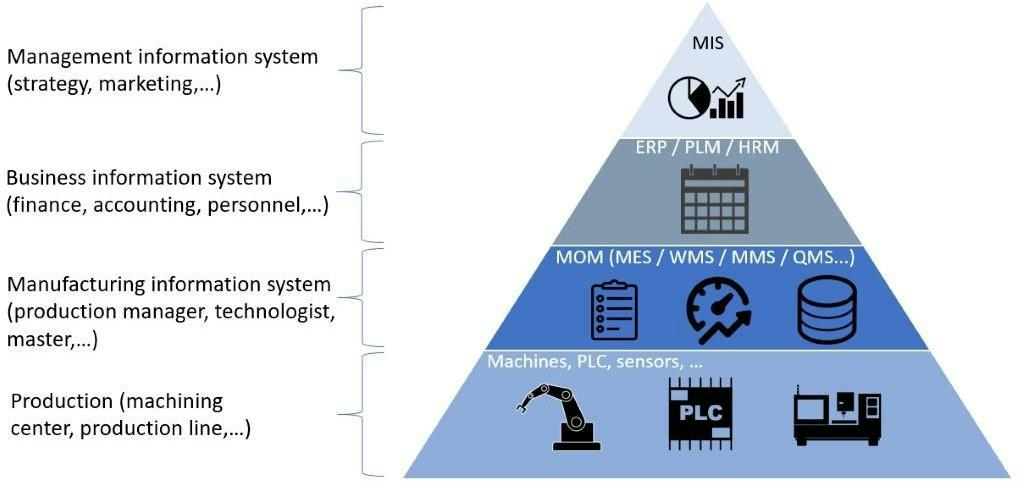
\includegraphics[width=441.55pt,height=207.4pt]{latexImage_7ae3c0ecdbf2ffea20e365934ceb1b9e.png}}
\end{picture}
\newpage
\begin{tikzpicture}[overlay]\path(0pt,0pt);\end{tikzpicture}
\begin{picture}(-5,0)(2.5,0)
\put(500.26,-727.616){\fontsize{12}{1}\usefont{T1}{ptm}{m}{n}\selectfont\color{color_29791}9}
\put(506.02,-727.616){\fontsize{12}{1}\usefont{T1}{ptm}{m}{n}\selectfont\color{color_29791} }
\put(63.024,-726.896){\fontsize{9.96}{1}\usefont{T1}{ptm}{m}{n}\selectfont\color{color_29791} }
\put(85.05,-620.83){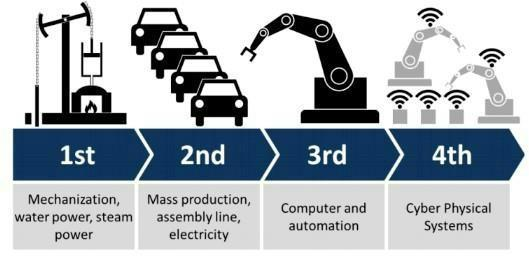
\includegraphics[width=396.1pt,height=191.98pt]{latexImage_69ae402e87e7e49732d944940b2ebb16.png}}
\put(82.944,-72.44){\fontsize{12}{1}\usefont{T1}{ptm}{m}{n}\selectfont\color{color_29791}MES}
\put(107.652,-72.44){\fontsize{12}{1}\usefont{T1}{ptm}{m}{n}\selectfont\color{color_29791}A}
\put(116.3,-72.44){\fontsize{12}{1}\usefont{T1}{ptm}{m}{n}\selectfont\color{color_29791}  }
\put(125.06,-72.44){\fontsize{12}{1}\usefont{T1}{ptm}{m}{n}\selectfont\color{color_29791}I}
\put(128.9,-72.44){\fontsize{12}{1}\usefont{T1}{ptm}{m}{n}\selectfont\color{color_29791}nter}
\put(147.5,-72.44){\fontsize{12}{1}\usefont{T1}{ptm}{m}{n}\selectfont\color{color_29791}n}
\put(153.608,-72.44){\fontsize{12}{1}\usefont{T1}{ptm}{m}{n}\selectfont\color{color_29791}a}
\put(158.888,-72.44){\fontsize{12}{1}\usefont{T1}{ptm}{m}{n}\selectfont\color{color_29791}ti}
\put(165.596,-72.44){\fontsize{12}{1}\usefont{T1}{ptm}{m}{n}\selectfont\color{color_29791}ona}
\put(182.876,-72.44){\fontsize{12}{1}\usefont{T1}{ptm}{m}{n}\selectfont\color{color_29791}l}
\put(186.29,-72.44){\fontsize{12}{1}\usefont{T1}{ptm}{m}{n}\selectfont\color{color_29791}(}
\put(198.29,-72.44){\fontsize{12}{1}\usefont{T1}{ptm}{m}{n}\selectfont\color{color_29791}1997}
\put(222.29,-72.44){\fontsize{12}{1}\usefont{T1}{ptm}{m}{n}\selectfont\color{color_29791}年)將}
\put(258.29,-72.44){\fontsize{12}{1}\usefont{T1}{ptm}{m}{n}\selectfont\color{color_29791}MES}
\put(283.01,-72.44){\fontsize{12}{1}\usefont{T1}{ptm}{m}{n}\selectfont\color{color_29791}的功能分為}
\put(343.03,-72.44){\fontsize{12}{1}\usefont{T1}{ptm}{m}{n}\selectfont\color{color_29791}11}
\put(355.03,-72.44){\fontsize{12}{1}\usefont{T1}{ptm}{m}{n}\selectfont\color{color_29791}類}
\put(367.03,-72.44){\fontsize{12}{1}\usefont{T1}{ptm}{m}{n}\selectfont\color{color_29791};}
\put(370.39,-72.44){\fontsize{12}{1}\usefont{T1}{ptm}{m}{n}\selectfont\color{color_29791}此外,}
\put(406.39,-72.44){\fontsize{12}{1}\usefont{T1}{ptm}{m}{n}\selectfont\color{color_29791}I}
\put(410.23,-72.44){\fontsize{12}{1}\usefont{T1}{ptm}{m}{n}\selectfont\color{color_29791}S}
\put(416.938,-72.44){\fontsize{12}{1}\usefont{T1}{ptm}{m}{n}\selectfont\color{color_29791}A95}
\put(437.71,-72.44){\fontsize{12}{1}\usefont{T1}{ptm}{m}{n}\selectfont\color{color_29791}  }
\put(446.38,-72.44){\fontsize{12}{1}\usefont{T1}{ptm}{m}{n}\selectfont\color{color_29791}–}
\put(453.7,-72.44){\fontsize{12}{1}\usefont{T1}{ptm}{m}{n}\selectfont\color{color_29791}  }
\put(462.46,-72.44){\fontsize{12}{1}\usefont{T1}{ptm}{m}{n}\selectfont\color{color_29791}I}
\put(466.3,-72.44){\fontsize{12}{1}\usefont{T1}{ptm}{m}{n}\selectfont\color{color_29791}E}
\put(473.5,-72.44){\fontsize{12}{1}\usefont{T1}{ptm}{m}{n}\selectfont\color{color_29791}C}
\put(481.42,-72.44){\fontsize{12}{1}\usefont{T1}{ptm}{m}{n}\selectfont\color{color_29791}6}
\put(487.3,-72.44){\fontsize{12}{1}\usefont{T1}{ptm}{m}{n}\selectfont\color{color_29791}2}
\put(493.18,-72.44){\fontsize{12}{1}\usefont{T1}{ptm}{m}{n}\selectfont\color{color_29791}26}
\put(505.06,-72.44){\fontsize{12}{1}\usefont{T1}{ptm}{m}{n}\selectfont\color{color_29791}4}
\put(511.06,-72.44){\fontsize{12}{1}\usefont{T1}{ptm}{m}{n}\selectfont\color{color_29791} }
\put(69.384,-90.21997){\fontsize{12}{1}\usefont{T1}{ptm}{m}{n}\selectfont\color{color_29791}(}
\put(81.264,-90.21997){\fontsize{12}{1}\usefont{T1}{ptm}{m}{n}\selectfont\color{color_29791}2013}
\put(104.78,-90.21997){\fontsize{12}{1}\usefont{T1}{ptm}{m}{n}\selectfont\color{color_29791})}
\put(116.78,-90.21997){\fontsize{12}{1}\usefont{T1}{ptm}{m}{n}\selectfont\color{color_29791} }
\put(69.384,-108.1){\fontsize{12}{1}\usefont{T1}{ptm}{m}{n}\selectfont\color{color_29791}標準中列出了每個}
\put(164.532,-108.1){\fontsize{12}{1}\usefont{T1}{ptm}{m}{n}\selectfont\color{color_29791}企業}
\put(188.4,-108.1){\fontsize{12}{1}\usefont{T1}{ptm}{m}{n}\selectfont\color{color_29791}層以及每種資訊系}
\put(283.548,-108.1){\fontsize{12}{1}\usefont{T1}{ptm}{m}{n}\selectfont\color{color_29791}統的}
\put(307.416,-108.1){\fontsize{12}{1}\usefont{T1}{ptm}{m}{n}\selectfont\color{color_29791}任務。該標準還為}
\put(402.564,-108.1){\fontsize{12}{1}\usefont{T1}{ptm}{m}{n}\selectfont\color{color_29791}資訊}
\put(426.432,-108.1){\fontsize{12}{1}\usefont{T1}{ptm}{m}{n}\selectfont\color{color_29791}系統之間交換}
\put(69.384,-125.86){\fontsize{12}{1}\usefont{T1}{ptm}{m}{n}\selectfont\color{color_29791}的數據結構提供了}
\put(164.532,-125.86){\fontsize{12}{1}\usefont{T1}{ptm}{m}{n}\selectfont\color{color_29791}定義}
\put(188.4,-125.86){\fontsize{12}{1}\usefont{T1}{ptm}{m}{n}\selectfont\color{color_29791},旨在加強其集成}
\put(283.49,-125.86){\fontsize{12}{1}\usefont{T1}{ptm}{m}{n}\selectfont\color{color_29791};}
\put(286.85,-125.86){\fontsize{12}{1}\usefont{T1}{ptm}{m}{n}\selectfont\color{color_29791}然}
\put(298.73,-125.86){\fontsize{12}{1}\usefont{T1}{ptm}{m}{n}\selectfont\color{color_29791}而,}
\put(322.61,-125.86){\fontsize{12}{1}\usefont{T1}{ptm}{m}{n}\selectfont\color{color_29791}它}
\put(334.49,-125.86){\fontsize{12}{1}\usefont{T1}{ptm}{m}{n}\selectfont\color{color_29791}主}
\put(346.37,-125.86){\fontsize{12}{1}\usefont{T1}{ptm}{m}{n}\selectfont\color{color_29791}要}
\put(358.25,-125.86){\fontsize{12}{1}\usefont{T1}{ptm}{m}{n}\selectfont\color{color_29791}關}
\put(370.13,-125.86){\fontsize{12}{1}\usefont{T1}{ptm}{m}{n}\selectfont\color{color_29791}注}
\put(382.03,-125.86){\fontsize{12}{1}\usefont{T1}{ptm}{m}{n}\selectfont\color{color_29791}E}
\put(389.23,-125.86){\fontsize{12}{1}\usefont{T1}{ptm}{m}{n}\selectfont\color{color_29791}R}
\put(397.15,-125.86){\fontsize{12}{1}\usefont{T1}{ptm}{m}{n}\selectfont\color{color_29791}P}
\put(403.75,-125.86){\fontsize{12}{1}\usefont{T1}{ptm}{m}{n}\selectfont\color{color_29791}-}
\put(407.71,-125.86){\fontsize{12}{1}\usefont{T1}{ptm}{m}{n}\selectfont\color{color_29791}M}
\put(418.27,-125.86){\fontsize{12}{1}\usefont{T1}{ptm}{m}{n}\selectfont\color{color_29791}E}
\put(425.47,-125.86){\fontsize{12}{1}\usefont{T1}{ptm}{m}{n}\selectfont\color{color_29791}S}
\put(432.19,-125.86){\fontsize{12}{1}\usefont{T1}{ptm}{m}{n}\selectfont\color{color_29791}-}
\put(436.03,-125.86){\fontsize{12}{1}\usefont{T1}{ptm}{m}{n}\selectfont\color{color_29791} }
\put(69.384,-143.74){\fontsize{12}{1}\usefont{T1}{ptm}{m}{n}\selectfont\color{color_29791}車間集成(}
\put(129.38,-143.74){\fontsize{12}{1}\usefont{T1}{ptm}{m}{n}\selectfont\color{color_29791}D'A}
\put(148.82,-143.74){\fontsize{12}{1}\usefont{T1}{ptm}{m}{n}\selectfont\color{color_29791}ntoni}
\put(173.528,-143.74){\fontsize{12}{1}\usefont{T1}{ptm}{m}{n}\selectfont\color{color_29791}o}
\put(179.57,-143.74){\fontsize{12}{1}\usefont{T1}{ptm}{m}{n}\selectfont\color{color_29791} }
\put(182.33,-143.74){\fontsize{12}{1}\usefont{T1}{ptm}{m}{n}\selectfont\color{color_29791}et}
\put(191.09,-143.74){\fontsize{12}{1}\usefont{T1}{ptm}{m}{n}\selectfont\color{color_29791} }
\put(194.09,-143.74){\fontsize{12}{1}\usefont{T1}{ptm}{m}{n}\selectfont\color{color_29791}a}
\put(199.37,-143.74){\fontsize{12}{1}\usefont{T1}{ptm}{m}{n}\selectfont\color{color_29791}l.}
\put(205.73,-143.74){\fontsize{12}{1}\usefont{T1}{ptm}{m}{n}\selectfont\color{color_29791},}
\put(216.17,-143.74){\fontsize{12}{1}\usefont{T1}{ptm}{m}{n}\selectfont\color{color_29791} }
\put(220.61,-143.74){\fontsize{12}{1}\usefont{T1}{ptm}{m}{n}\selectfont\color{color_29791}2015}
\put(244.61,-143.74){\fontsize{12}{1}\usefont{T1}{ptm}{m}{n}\selectfont\color{color_29791})}
\put(256.61,-143.74){\fontsize{12}{1}\usefont{T1}{ptm}{m}{n}\selectfont\color{color_29791}。}
\put(268.25,-143.74){\fontsize{12}{1}\usefont{T1}{ptm}{m}{n}\selectfont\color{color_29791} }
\put(63.024,-161.98){\fontsize{12}{1}\usefont{T1}{ptm}{m}{n}\selectfont\color{color_29791} }
\put(82.944,-177.58){\fontsize{12}{1}\usefont{T1}{ptm}{m}{n}\selectfont\color{color_29791}相比之}
\put(118.94,-177.58){\fontsize{12}{1}\usefont{T1}{ptm}{m}{n}\selectfont\color{color_29791}下}
\put(130.94,-177.58){\fontsize{12}{1}\usefont{T1}{ptm}{m}{n}\selectfont\color{color_29791},}
\put(142.94,-177.58){\fontsize{12}{1}\usefont{T1}{ptm}{m}{n}\selectfont\color{color_29791}P}
\put(149.78,-177.58){\fontsize{12}{1}\usefont{T1}{ptm}{m}{n}\selectfont\color{color_29791}L}
\put(156.86,-177.58){\fontsize{12}{1}\usefont{T1}{ptm}{m}{n}\selectfont\color{color_29791}M}
\put(167.42,-177.58){\fontsize{12}{1}\usefont{T1}{ptm}{m}{n}\selectfont\color{color_29791} }
\put(265.37,-177.58){\fontsize{12}{1}\usefont{T1}{ptm}{m}{n}\selectfont\color{color_29791}研究要新得多,而}
\put(361.39,-177.58){\fontsize{12}{1}\usefont{T1}{ptm}{m}{n}\selectfont\color{color_29791} }
\put(459.1,-177.58){\fontsize{12}{1}\usefont{T1}{ptm}{m}{n}\selectfont\color{color_29791}P}
\put(465.82,-177.58){\fontsize{12}{1}\usefont{T1}{ptm}{m}{n}\selectfont\color{color_29791}L}
\put(472.78,-177.58){\fontsize{12}{1}\usefont{T1}{ptm}{m}{n}\selectfont\color{color_29791}M}
\put(483.46,-177.58){\fontsize{12}{1}\usefont{T1}{ptm}{m}{n}\selectfont\color{color_29791}-}
\put(487.3,-177.58){\fontsize{12}{1}\usefont{T1}{ptm}{m}{n}\selectfont\color{color_29791}M}
\put(497.86,-177.58){\fontsize{12}{1}\usefont{T1}{ptm}{m}{n}\selectfont\color{color_29791}E}
\put(505.06,-177.58){\fontsize{12}{1}\usefont{T1}{ptm}{m}{n}\selectfont\color{color_29791}S}
\put(69.384,-195.46){\fontsize{12}{1}\usefont{T1}{ptm}{m}{n}\selectfont\color{color_29791}集成是這項工作的主要重點,更是如此。(第}
\put(309.43,-195.46){\fontsize{12}{1}\usefont{T1}{ptm}{m}{n}\selectfont\color{color_29791}3}
\put(315.43,-195.46){\fontsize{12}{1}\usefont{T1}{ptm}{m}{n}\selectfont\color{color_29791}章)介紹了這種整合的挑戰和最新的}
\put(69.384,-213.34){\fontsize{12}{1}\usefont{T1}{ptm}{m}{n}\selectfont\color{color_29791}技}
\put(81.384,-213.34){\fontsize{12}{1}\usefont{T1}{ptm}{m}{n}\selectfont\color{color_29791}術}
\put(93.38,-213.34){\fontsize{12}{1}\usefont{T1}{ptm}{m}{n}\selectfont\color{color_29791},以及它背後的理論結構。現在,我只想指出,由於}
\put(369.43,-213.34){\fontsize{12}{1}\usefont{T1}{ptm}{m}{n}\selectfont\color{color_29791}ME}
\put(387.43,-213.34){\fontsize{12}{1}\usefont{T1}{ptm}{m}{n}\selectfont\color{color_29791}S}
\put(394.15,-213.34){\fontsize{12}{1}\usefont{T1}{ptm}{m}{n}\selectfont\color{color_29791}提供反}
\put(430.03,-213.34){\fontsize{12}{1}\usefont{T1}{ptm}{m}{n}\selectfont\color{color_29791}饋,通過以檔}
\put(69.384,-231.34){\fontsize{12}{1}\usefont{T1}{ptm}{m}{n}\selectfont\color{color_29791}的形式生成資訊來協調更改並驗證結果,而}
\put(297.41,-231.34){\fontsize{12}{1}\usefont{T1}{ptm}{m}{n}\selectfont\color{color_29791}P}
\put(304.25,-231.34){\fontsize{12}{1}\usefont{T1}{ptm}{m}{n}\selectfont\color{color_29791}L}
\put(311.47,-231.34){\fontsize{12}{1}\usefont{T1}{ptm}{m}{n}\selectfont\color{color_29791}M}
\put(322.15,-231.34){\fontsize{12}{1}\usefont{T1}{ptm}{m}{n}\selectfont\color{color_29791}則專注於按檔組織跟蹤更改,因此}
\put(502.18,-231.34){\fontsize{12}{1}\usefont{T1}{ptm}{m}{n}\selectfont\color{color_29791}P }
\put(69.384,-249.25){\fontsize{12}{1}\usefont{T1}{ptm}{m}{n}\selectfont\color{color_29791}L}
\put(76.584,-249.25){\fontsize{12}{1}\usefont{T1}{ptm}{m}{n}\selectfont\color{color_29791}M}
\put(87.26,-249.25){\fontsize{12}{1}\usefont{T1}{ptm}{m}{n}\selectfont\color{color_29791}-}
\put(91.22,-249.25){\fontsize{12}{1}\usefont{T1}{ptm}{m}{n}\selectfont\color{color_29791}ME}
\put(109.22,-249.25){\fontsize{12}{1}\usefont{T1}{ptm}{m}{n}\selectfont\color{color_29791}S}
\put(115.94,-249.25){\fontsize{12}{1}\usefont{T1}{ptm}{m}{n}\selectfont\color{color_29791}集成肯定具}
\put(175.94,-249.25){\fontsize{12}{1}\usefont{T1}{ptm}{m}{n}\selectfont\color{color_29791}有}
\put(187.97,-249.25){\fontsize{12}{1}\usefont{T1}{ptm}{m}{n}\selectfont\color{color_29791}價值。}
\put(223.97,-249.25){\fontsize{12}{1}\usefont{T1}{ptm}{m}{n}\selectfont\color{color_29791} }
\put(63.024,-277.57){\fontsize{12}{1}\usefont{T1}{ptm}{m}{n}\selectfont\color{color_29791} }
\put(87.38,-298.93){\fontsize{14.04}{1}\usefont{T1}{ptm}{b}{n}\selectfont\color{color_29791}2}
\put(94.44212,-298.93){\fontsize{14.04}{1}\usefont{T1}{ptm}{b}{n}\selectfont\color{color_29791}.4.}
\put(108.38,-298.93){\fontsize{14.04}{1}\usefont{T1}{ptm}{b}{n}\selectfont\color{color_29791} }
\put(111.74,-298.93){\fontsize{14.04}{1}\usefont{T1}{ptm}{b}{n}\selectfont\color{color_29791}工業}
\put(139.82,-298.93){\fontsize{14.04}{1}\usefont{T1}{ptm}{b}{n}\selectfont\color{color_29791}4}
\put(146.6575,-298.93){\fontsize{14.04}{1}\usefont{T1}{ptm}{b}{n}\selectfont\color{color_29791}.}
\put(149.7744,-298.93){\fontsize{14.04}{1}\usefont{T1}{ptm}{b}{n}\selectfont\color{color_29791}0}
\put(156.5,-298.93){\fontsize{14.04}{1}\usefont{T1}{ptm}{b}{n}\selectfont\color{color_29791} }
\put(82.944,-332.65){\fontsize{12}{1}\usefont{T1}{ptm}{m}{n}\selectfont\color{color_29791}工}
\put(94.94,-332.65){\fontsize{12}{1}\usefont{T1}{ptm}{m}{n}\selectfont\color{color_29791}業}
\put(106.46,-332.65){\fontsize{12}{1}\usefont{T1}{ptm}{m}{n}\selectfont\color{color_29791} }
\put(497.5,-332.65){\fontsize{12}{1}\usefont{T1}{ptm}{m}{n}\selectfont\color{color_29791}4.0}
\put(511.78,-332.65){\fontsize{12}{1}\usefont{T1}{ptm}{m}{n}\selectfont\color{color_29791} }
\put(69.384,-350.53){\fontsize{12}{1}\usefont{T1}{ptm}{m}{n}\selectfont\color{color_29791}一詞在現代文獻中一再}
\put(189.492,-350.53){\fontsize{12}{1}\usefont{T1}{ptm}{m}{n}\selectfont\color{color_29791}被提及,作為生產發展}
\put(309.6,-350.53){\fontsize{12}{1}\usefont{T1}{ptm}{m}{n}\selectfont\color{color_29791}的下一步或當前步驟。}
\put(429.708,-350.53){\fontsize{12}{1}\usefont{T1}{ptm}{m}{n}\selectfont\color{color_29791}它代表了第四}
\put(69.384,-368.41){\fontsize{12}{1}\usefont{T1}{ptm}{m}{n}\selectfont\color{color_29791}次工業革命,第一次工}
\put(189.492,-368.41){\fontsize{12}{1}\usefont{T1}{ptm}{m}{n}\selectfont\color{color_29791}業革命以採用蒸汽動力}
\put(309.6,-368.41){\fontsize{12}{1}\usefont{T1}{ptm}{m}{n}\selectfont\color{color_29791}為標誌,第二次以主要}
\put(429.708,-368.41){\fontsize{12}{1}\usefont{T1}{ptm}{m}{n}\selectfont\color{color_29791}使用電力為標}
\put(69.384,-386.29){\fontsize{12}{1}\usefont{T1}{ptm}{m}{n}\selectfont\color{color_29791}誌,第三次以數位}
\put(164.532,-386.29){\fontsize{12}{1}\usefont{T1}{ptm}{m}{n}\selectfont\color{color_29791}技術}
\put(188.4,-386.29){\fontsize{12}{1}\usefont{T1}{ptm}{m}{n}\selectfont\color{color_29791}的實施為特徵。圖}
\put(283.61,-386.29){\fontsize{12}{1}\usefont{T1}{ptm}{m}{n}\selectfont\color{color_29791}5}
\put(289.49,-386.29){\fontsize{12}{1}\usefont{T1}{ptm}{m}{n}\selectfont\color{color_29791}很好}
\put(313.37,-386.29){\fontsize{12}{1}\usefont{T1}{ptm}{m}{n}\selectfont\color{color_29791}地}
\put(325.25,-386.29){\fontsize{12}{1}\usefont{T1}{ptm}{m}{n}\selectfont\color{color_29791}代}
\put(337.13,-386.29){\fontsize{12}{1}\usefont{T1}{ptm}{m}{n}\selectfont\color{color_29791}表}
\put(349.01,-386.29){\fontsize{12}{1}\usefont{T1}{ptm}{m}{n}\selectfont\color{color_29791}了}
\put(360.89,-386.29){\fontsize{12}{1}\usefont{T1}{ptm}{m}{n}\selectfont\color{color_29791}工}
\put(372.77,-386.29){\fontsize{12}{1}\usefont{T1}{ptm}{m}{n}\selectfont\color{color_29791}業}
\put(384.65,-386.29){\fontsize{12}{1}\usefont{T1}{ptm}{m}{n}\selectfont\color{color_29791}革命}
\put(408.53,-386.29){\fontsize{12}{1}\usefont{T1}{ptm}{m}{n}\selectfont\color{color_29791}的進}
\put(432.41,-386.29){\fontsize{12}{1}\usefont{T1}{ptm}{m}{n}\selectfont\color{color_29791}展}
\put(444.29,-386.29){\fontsize{12}{1}\usefont{T1}{ptm}{m}{n}\selectfont\color{color_29791}。}
\put(456.34,-386.29){\fontsize{12}{1}\usefont{T1}{ptm}{m}{n}\selectfont\color{color_29791} }
\put(63.024,-402.13){\fontsize{9.96}{1}\usefont{T1}{ptm}{m}{n}\selectfont\color{color_29791} }
\put(63.024,-424.95){\fontsize{9.96}{1}\usefont{T1}{ptm}{m}{n}\selectfont\color{color_29791} }
\put(165.02,-637.38){\fontsize{12}{1}\usefont{T1}{ptm}{b}{n}\selectfont\color{color_29791}圖}
\put(176.9,-637.38){\fontsize{12}{1}\usefont{T1}{ptm}{b}{n}\selectfont\color{color_29791}5}
\put(182.81,-637.38){\fontsize{12}{1}\usefont{T1}{ptm}{b}{n}\selectfont\color{color_29791}行}
\put(194.69,-637.38){\fontsize{12}{1}\usefont{T1}{ptm}{b}{n}\selectfont\color{color_29791}業}
\put(206.57,-637.38){\fontsize{12}{1}\usefont{T1}{ptm}{b}{n}\selectfont\color{color_29791}演}
\put(218.45,-637.38){\fontsize{12}{1}\usefont{T1}{ptm}{b}{n}\selectfont\color{color_29791}變}
\put(230.33,-637.38){\fontsize{12}{1}\usefont{T1}{ptm}{b}{n}\selectfont\color{color_29791}(}
\put(242.21,-637.38){\fontsize{12}{1}\usefont{T1}{ptm}{b}{n}\selectfont\color{color_29791}改編}
\put(266.09,-637.38){\fontsize{12}{1}\usefont{T1}{ptm}{b}{n}\selectfont\color{color_29791}自}
\put(277.97,-637.38){\fontsize{12}{1}\usefont{T1}{ptm}{b}{n}\selectfont\color{color_29791}S}
\put(284.678,-637.38){\fontsize{12}{1}\usefont{T1}{ptm}{b}{n}\selectfont\color{color_29791}T}
\put(292.598,-637.38){\fontsize{12}{1}\usefont{T1}{ptm}{b}{n}\selectfont\color{color_29791}A}
\put(301.118,-637.38){\fontsize{12}{1}\usefont{T1}{ptm}{b}{n}\selectfont\color{color_29791}N}
\put(309.638,-637.38){\fontsize{12}{1}\usefont{T1}{ptm}{b}{n}\selectfont\color{color_29791}C}
\put(318.158,-637.38){\fontsize{12}{1}\usefont{T1}{ptm}{b}{n}\selectfont\color{color_29791}I}
\put(322.718,-637.38){\fontsize{12}{1}\usefont{T1}{ptm}{b}{n}\selectfont\color{color_29791}O}
\put(331.958,-637.38){\fontsize{12}{1}\usefont{T1}{ptm}{b}{n}\selectfont\color{color_29791}IU}
\put(345.19,-637.38){\fontsize{12}{1}\usefont{T1}{ptm}{b}{n}\selectfont\color{color_29791} }
\put(348.31,-637.38){\fontsize{12}{1}\usefont{T1}{ptm}{b}{n}\selectfont\color{color_29791}A}
\put(356.83,-637.38){\fontsize{12}{1}\usefont{T1}{ptm}{b}{n}\selectfont\color{color_29791}l}
\put(360.07,-637.38){\fontsize{12}{1}\usefont{T1}{ptm}{b}{n}\selectfont\color{color_29791}i}
\put(363.31,-637.38){\fontsize{12}{1}\usefont{T1}{ptm}{b}{n}\selectfont\color{color_29791}n}
\put(369.91,-637.38){\fontsize{12}{1}\usefont{T1}{ptm}{b}{n}\selectfont\color{color_29791},}
\put(381.79,-637.38){\fontsize{12}{1}\usefont{T1}{ptm}{b}{n}\selectfont\color{color_29791}2017}
\put(405.43,-637.38){\fontsize{12}{1}\usefont{T1}{ptm}{b}{n}\selectfont\color{color_29791})}
\put(417.31,-637.38){\fontsize{12}{1}\usefont{T1}{ptm}{b}{n}\selectfont\color{color_29791} }
\put(82.944,-670.14){\fontsize{12}{1}\usefont{T1}{ptm}{m}{n}\selectfont\color{color_29791}從廣義上講,第四次工}
\put(203.052,-670.14){\fontsize{12}{1}\usefont{T1}{ptm}{m}{n}\selectfont\color{color_29791}業革命最終以數位連接}
\put(323.16,-670.14){\fontsize{12}{1}\usefont{T1}{ptm}{m}{n}\selectfont\color{color_29791}與生產之間的全面融合}
\put(443.268,-670.14){\fontsize{12}{1}\usefont{T1}{ptm}{m}{n}\selectfont\color{color_29791}為標誌。眾}
\put(69.384,-687.776){\fontsize{12}{1}\usefont{T1}{ptm}{m}{n}\selectfont\color{color_29791}所周知}
\put(105.492,-687.776){\fontsize{12}{1}\usefont{T1}{ptm}{m}{n}\selectfont\color{color_29791},數}
\put(129.6,-687.776){\fontsize{12}{1}\usefont{T1}{ptm}{m}{n}\selectfont\color{color_29791}位網}
\put(153.708,-687.776){\fontsize{12}{1}\usefont{T1}{ptm}{m}{n}\selectfont\color{color_29791}路的}
\put(177.816,-687.776){\fontsize{12}{1}\usefont{T1}{ptm}{m}{n}\selectfont\color{color_29791}發}
\put(189.924,-687.776){\fontsize{12}{1}\usefont{T1}{ptm}{m}{n}\selectfont\color{color_29791}展是維}
\put(226.032,-687.776){\fontsize{12}{1}\usefont{T1}{ptm}{m}{n}\selectfont\color{color_29791}持現}
\put(250.14,-687.776){\fontsize{12}{1}\usefont{T1}{ptm}{m}{n}\selectfont\color{color_29791}代世}
\put(274.248,-687.776){\fontsize{12}{1}\usefont{T1}{ptm}{m}{n}\selectfont\color{color_29791}界的}
\put(298.356,-687.776){\fontsize{12}{1}\usefont{T1}{ptm}{m}{n}\selectfont\color{color_29791}關}
\put(310.464,-687.776){\fontsize{12}{1}\usefont{T1}{ptm}{m}{n}\selectfont\color{color_29791}鍵技術}
\put(346.572,-687.776){\fontsize{12}{1}\usefont{T1}{ptm}{m}{n}\selectfont\color{color_29791}。它}
\put(370.68,-687.776){\fontsize{12}{1}\usefont{T1}{ptm}{m}{n}\selectfont\color{color_29791}改變}
\put(394.788,-687.776){\fontsize{12}{1}\usefont{T1}{ptm}{m}{n}\selectfont\color{color_29791}了人}
\put(418.896,-687.776){\fontsize{12}{1}\usefont{T1}{ptm}{m}{n}\selectfont\color{color_29791}類}
\put(431.004,-687.776){\fontsize{12}{1}\usefont{T1}{ptm}{m}{n}\selectfont\color{color_29791}互動和}
\put(467.112,-687.776){\fontsize{12}{1}\usefont{T1}{ptm}{m}{n}\selectfont\color{color_29791}做生意}
\put(69.384,-705.536){\fontsize{12}{1}\usefont{T1}{ptm}{m}{n}\selectfont\color{color_29791}的方式}
\put(105.264,-705.536){\fontsize{12}{1}\usefont{T1}{ptm}{m}{n}\selectfont\color{color_29791}。然而}
\put(141.144,-705.536){\fontsize{12}{1}\usefont{T1}{ptm}{m}{n}\selectfont\color{color_29791},目}
\put(165.024,-705.536){\fontsize{12}{1}\usefont{T1}{ptm}{m}{n}\selectfont\color{color_29791}前應}
\put(188.904,-705.536){\fontsize{12}{1}\usefont{T1}{ptm}{m}{n}\selectfont\color{color_29791}用於工}
\put(224.784,-705.536){\fontsize{12}{1}\usefont{T1}{ptm}{m}{n}\selectfont\color{color_29791}業的水}
\put(260.664,-705.536){\fontsize{12}{1}\usefont{T1}{ptm}{m}{n}\selectfont\color{color_29791}準是}
\put(284.544,-705.536){\fontsize{12}{1}\usefont{T1}{ptm}{m}{n}\selectfont\color{color_29791}否構}
\put(308.424,-705.536){\fontsize{12}{1}\usefont{T1}{ptm}{m}{n}\selectfont\color{color_29791}成工業}
\put(344.304,-705.536){\fontsize{12}{1}\usefont{T1}{ptm}{m}{n}\selectfont\color{color_29791}革命仍}
\put(380.1841,-705.536){\fontsize{12}{1}\usefont{T1}{ptm}{m}{n}\selectfont\color{color_29791}然不}
\put(404.0641,-705.536){\fontsize{12}{1}\usefont{T1}{ptm}{m}{n}\selectfont\color{color_29791}確定}
\put(427.9441,-705.536){\fontsize{12}{1}\usefont{T1}{ptm}{m}{n}\selectfont\color{color_29791},因為}
\put(463.8241,-705.536){\fontsize{12}{1}\usefont{T1}{ptm}{m}{n}\selectfont\color{color_29791}在所有}
\put(499.78,-705.536){\fontsize{12}{1}\usefont{T1}{ptm}{m}{n}\selectfont\color{color_29791} }
\end{picture}
\newpage
\begin{tikzpicture}[overlay]\path(0pt,0pt);\end{tikzpicture}
\begin{picture}(-5,0)(2.5,0)
\put(500.26,-727.616){\fontsize{12}{1}\usefont{T1}{ptm}{m}{n}\selectfont\color{color_29791}10}
\put(511.78,-727.616){\fontsize{12}{1}\usefont{T1}{ptm}{m}{n}\selectfont\color{color_29791} }
\put(63.024,-726.896){\fontsize{9.96}{1}\usefont{T1}{ptm}{m}{n}\selectfont\color{color_29791} }
\put(69.384,-72.44){\fontsize{12}{1}\usefont{T1}{ptm}{m}{n}\selectfont\color{color_29791}其他革命中,都以}
\put(164.532,-72.44){\fontsize{12}{1}\usefont{T1}{ptm}{m}{n}\selectfont\color{color_29791}產量}
\put(188.4,-72.44){\fontsize{12}{1}\usefont{T1}{ptm}{m}{n}\selectfont\color{color_29791}的急劇增加為標誌}
\put(283.548,-72.44){\fontsize{12}{1}\usefont{T1}{ptm}{m}{n}\selectfont\color{color_29791},而}
\put(307.416,-72.44){\fontsize{12}{1}\usefont{T1}{ptm}{m}{n}\selectfont\color{color_29791}這一次尚未發生。}
\put(402.564,-72.44){\fontsize{12}{1}\usefont{T1}{ptm}{m}{n}\selectfont\color{color_29791}事實}
\put(426.432,-72.44){\fontsize{12}{1}\usefont{T1}{ptm}{m}{n}\selectfont\color{color_29791}上,我們仍有}
\put(69.384,-90.46002){\fontsize{12}{1}\usefont{T1}{ptm}{m}{n}\selectfont\color{color_29791}待達成工業}
\put(128.78,-90.46002){\fontsize{12}{1}\usefont{T1}{ptm}{m}{n}\selectfont\color{color_29791}4.0}
\put(143.54,-90.46002){\fontsize{12}{1}\usefont{T1}{ptm}{m}{n}\selectfont\color{color_29791}的}
\put(155.42,-90.46002){\fontsize{12}{1}\usefont{T1}{ptm}{m}{n}\selectfont\color{color_29791}共}
\put(167.3,-90.46002){\fontsize{12}{1}\usefont{T1}{ptm}{m}{n}\selectfont\color{color_29791}同}
\put(179.18,-90.46002){\fontsize{12}{1}\usefont{T1}{ptm}{m}{n}\selectfont\color{color_29791}定義}
\put(203.06,-90.46002){\fontsize{12}{1}\usefont{T1}{ptm}{m}{n}\selectfont\color{color_29791}。}
\put(214.97,-90.46002){\fontsize{12}{1}\usefont{T1}{ptm}{m}{n}\selectfont\color{color_29791} }
\put(63.024,-108.58){\fontsize{12}{1}\usefont{T1}{ptm}{m}{n}\selectfont\color{color_29791} }
\put(83.664,-124.06){\fontsize{12}{1}\usefont{T1}{ptm}{m}{n}\selectfont\color{color_29791}然而,被廣泛接受的是,至少有}
\put(251.69,-124.06){\fontsize{15}{1}\usefont{T1}{ptm}{m}{n}\selectfont\color{color_29791} }
\put(263.69,-124.06){\fontsize{12}{1}\usefont{T1}{ptm}{m}{n}\selectfont\color{color_29791}3}
\put(269.09,-124.06){\fontsize{12}{1}\usefont{T1}{ptm}{m}{n}\selectfont\color{color_29791} }
\put(281.93,-124.06){\fontsize{12}{1}\usefont{T1}{ptm}{m}{n}\selectfont\color{color_29791}種技術是工業}
\put(353.95,-124.06){\fontsize{15}{1}\usefont{T1}{ptm}{m}{n}\selectfont\color{color_29791} }
\put(366.07,-124.06){\fontsize{12}{1}\usefont{T1}{ptm}{m}{n}\selectfont\color{color_29791}4.0}
\put(380.35,-124.06){\fontsize{12}{1}\usefont{T1}{ptm}{m}{n}\selectfont\color{color_29791} }
\put(393.19,-124.06){\fontsize{12}{1}\usefont{T1}{ptm}{m}{n}\selectfont\color{color_29791}的特徵。這些是物聯}
\put(501.22,-124.06){\fontsize{12}{1}\usefont{T1}{ptm}{m}{n}\selectfont\color{color_29791}網}
\put(512.74,-124.06){\fontsize{12}{1}\usefont{T1}{ptm}{m}{n}\selectfont\color{color_29791} }
\put(70.104,-141.82){\fontsize{12}{1}\usefont{T1}{ptm}{m}{n}\selectfont\color{color_29791}(}
\put(82.104,-141.82){\fontsize{12}{1}\usefont{T1}{ptm}{m}{n}\selectfont\color{color_29791}I}
\put(85.824,-141.82){\fontsize{12}{1}\usefont{T1}{ptm}{m}{n}\selectfont\color{color_29791}o}
\put(91.70399,-141.82){\fontsize{12}{1}\usefont{T1}{ptm}{m}{n}\selectfont\color{color_29791}T}
\put(98.9,-141.82){\fontsize{12}{1}\usefont{T1}{ptm}{m}{n}\selectfont\color{color_29791})}
\put(110.78,-141.82){\fontsize{12}{1}\usefont{T1}{ptm}{m}{n}\selectfont\color{color_29791}、雲}
\put(134.66,-141.82){\fontsize{12}{1}\usefont{T1}{ptm}{m}{n}\selectfont\color{color_29791}計}
\put(146.54,-141.82){\fontsize{12}{1}\usefont{T1}{ptm}{m}{n}\selectfont\color{color_29791}算}
\put(158.42,-141.82){\fontsize{12}{1}\usefont{T1}{ptm}{m}{n}\selectfont\color{color_29791}和}
\put(170.3,-141.82){\fontsize{12}{1}\usefont{T1}{ptm}{m}{n}\selectfont\color{color_29791}資訊}
\put(194.18,-141.82){\fontsize{12}{1}\usefont{T1}{ptm}{m}{n}\selectfont\color{color_29791}物}
\put(206.06,-141.82){\fontsize{12}{1}\usefont{T1}{ptm}{m}{n}\selectfont\color{color_29791}理}
\put(217.94,-141.82){\fontsize{12}{1}\usefont{T1}{ptm}{m}{n}\selectfont\color{color_29791}系}
\put(229.85,-141.82){\fontsize{12}{1}\usefont{T1}{ptm}{m}{n}\selectfont\color{color_29791}統}
\put(241.49,-141.82){\fontsize{12}{1}\usefont{T1}{ptm}{m}{n}\selectfont\color{color_29791} }
\put(467.98,-141.82){\fontsize{12}{1}\usefont{T1}{ptm}{m}{n}\selectfont\color{color_29791}(}
\put(479.86,-141.82){\fontsize{12}{1}\usefont{T1}{ptm}{m}{n}\selectfont\color{color_29791}C}
\put(487.78,-141.82){\fontsize{12}{1}\usefont{T1}{ptm}{m}{n}\selectfont\color{color_29791}P}
\put(494.38,-141.82){\fontsize{12}{1}\usefont{T1}{ptm}{m}{n}\selectfont\color{color_29791}S}
\put(500.98,-141.82){\fontsize{12}{1}\usefont{T1}{ptm}{m}{n}\selectfont\color{color_29791})}
\put(512.86,-141.82){\fontsize{12}{1}\usefont{T1}{ptm}{m}{n}\selectfont\color{color_29791} }
\put(69.384,-159.94){\fontsize{12}{1}\usefont{T1}{ptm}{m}{n}\selectfont\color{color_29791}的發展}
\put(105.264,-159.94){\fontsize{12}{1}\usefont{T1}{ptm}{m}{n}\selectfont\color{color_29791},其中}
\put(141.144,-159.94){\fontsize{12}{1}\usefont{T1}{ptm}{m}{n}\selectfont\color{color_29791}最後}
\put(165.024,-159.94){\fontsize{12}{1}\usefont{T1}{ptm}{m}{n}\selectfont\color{color_29791}一個}
\put(188.904,-159.94){\fontsize{12}{1}\usefont{T1}{ptm}{m}{n}\selectfont\color{color_29791}對於本}
\put(224.784,-159.94){\fontsize{12}{1}\usefont{T1}{ptm}{m}{n}\selectfont\color{color_29791}論文的}
\put(260.664,-159.94){\fontsize{12}{1}\usefont{T1}{ptm}{m}{n}\selectfont\color{color_29791}背景}
\put(284.544,-159.94){\fontsize{12}{1}\usefont{T1}{ptm}{m}{n}\selectfont\color{color_29791}尤為}
\put(308.424,-159.94){\fontsize{12}{1}\usefont{T1}{ptm}{m}{n}\selectfont\color{color_29791}重要。}
\put(344.35,-159.94){\fontsize{12}{1}\usefont{T1}{ptm}{m}{n}\selectfont\color{color_29791} }
\put(63.024,-178.06){\fontsize{12}{1}\usefont{T1}{ptm}{m}{n}\selectfont\color{color_29791} }
\put(82.944,-193.66){\fontsize{12}{1}\usefont{T1}{ptm}{m}{n}\selectfont\color{color_29791}C}
\put(90.972,-193.66){\fontsize{12}{1}\usefont{T1}{ptm}{m}{n}\selectfont\color{color_29791}P}
\put(97.68,-193.66){\fontsize{12}{1}\usefont{T1}{ptm}{m}{n}\selectfont\color{color_29791}S}
\put(104.42,-193.66){\fontsize{12}{1}\usefont{T1}{ptm}{m}{n}\selectfont\color{color_29791}是由一個真實實體}
\put(200.3,-193.66){\fontsize{12}{1}\usefont{T1}{ptm}{m}{n}\selectfont\color{color_29791}(例如,一台機器)及其相應的虛擬模型組成的系統}
\put(476.38,-193.66){\fontsize{12}{1}\usefont{T1}{ptm}{m}{n}\selectfont\color{color_29791}——}
\put(499.9,-193.66){\fontsize{12}{1}\usefont{T1}{ptm}{m}{n}\selectfont\color{color_29791} }
\put(69.384,-211.42){\fontsize{12}{1}\usefont{T1}{ptm}{m}{n}\selectfont\color{color_29791}嵌入所有模型以模仿真實對應物的行為}
\put(273.41,-211.42){\fontsize{12}{1}\usefont{T1}{ptm}{m}{n}\selectfont\color{color_29791}——}
\put(296.93,-211.42){\fontsize{12}{1}\usefont{T1}{ptm}{m}{n}\selectfont\color{color_29791} }
\put(69.384,-229.3){\fontsize{12}{1}\usefont{T1}{ptm}{m}{n}\selectfont\color{color_29791}能夠相互通信(}
\put(152.66,-229.3){\fontsize{12}{1}\usefont{T1}{ptm}{m}{n}\selectfont\color{color_29791}D}
\put(161.18,-229.3){\fontsize{12}{1}\usefont{T1}{ptm}{m}{n}\selectfont\color{color_29791}』}
\put(173.06,-229.3){\fontsize{12}{1}\usefont{T1}{ptm}{m}{n}\selectfont\color{color_29791}A}
\put(181.58,-229.3){\fontsize{12}{1}\usefont{T1}{ptm}{m}{n}\selectfont\color{color_29791}n}
\put(187.46,-229.3){\fontsize{12}{1}\usefont{T1}{ptm}{m}{n}\selectfont\color{color_29791}to}
\put(196.7,-229.3){\fontsize{12}{1}\usefont{T1}{ptm}{m}{n}\selectfont\color{color_29791}n}
\put(202.58,-229.3){\fontsize{12}{1}\usefont{T1}{ptm}{m}{n}\selectfont\color{color_29791}i}
\put(205.82,-229.3){\fontsize{12}{1}\usefont{T1}{ptm}{m}{n}\selectfont\color{color_29791}o}
\put(211.73,-229.3){\fontsize{12}{1}\usefont{T1}{ptm}{m}{n}\selectfont\color{color_29791}等人,}
\put(247.37,-229.3){\fontsize{12}{1}\usefont{T1}{ptm}{m}{n}\selectfont\color{color_29791}2}
\put(253.25,-229.3){\fontsize{12}{1}\usefont{T1}{ptm}{m}{n}\selectfont\color{color_29791}0}
\put(259.13,-229.3){\fontsize{12}{1}\usefont{T1}{ptm}{m}{n}\selectfont\color{color_29791}17}
\put(271.01,-229.3){\fontsize{12}{1}\usefont{T1}{ptm}{m}{n}\selectfont\color{color_29791})}
\put(282.89,-229.3){\fontsize{12}{1}\usefont{T1}{ptm}{m}{n}\selectfont\color{color_29791}。}
\put(294.77,-229.3){\fontsize{12}{1}\usefont{T1}{ptm}{m}{n}\selectfont\color{color_29791}這個}
\put(318.65,-229.3){\fontsize{12}{1}\usefont{T1}{ptm}{m}{n}\selectfont\color{color_29791}想}
\put(330.53,-229.3){\fontsize{12}{1}\usefont{T1}{ptm}{m}{n}\selectfont\color{color_29791}法}
\put(342.41,-229.3){\fontsize{12}{1}\usefont{T1}{ptm}{m}{n}\selectfont\color{color_29791}是}
\put(354.29,-229.3){\fontsize{12}{1}\usefont{T1}{ptm}{m}{n}\selectfont\color{color_29791},}
\put(366.17,-229.3){\fontsize{12}{1}\usefont{T1}{ptm}{m}{n}\selectfont\color{color_29791}如}
\put(378.05,-229.3){\fontsize{12}{1}\usefont{T1}{ptm}{m}{n}\selectfont\color{color_29791}果}
\put(389.9301,-229.3){\fontsize{12}{1}\usefont{T1}{ptm}{m}{n}\selectfont\color{color_29791}一個}
\put(413.8101,-229.3){\fontsize{12}{1}\usefont{T1}{ptm}{m}{n}\selectfont\color{color_29791}人要}
\put(437.6901,-229.3){\fontsize{12}{1}\usefont{T1}{ptm}{m}{n}\selectfont\color{color_29791}開}
\put(449.5701,-229.3){\fontsize{12}{1}\usefont{T1}{ptm}{m}{n}\selectfont\color{color_29791}發}
\put(461.4501,-229.3){\fontsize{12}{1}\usefont{T1}{ptm}{m}{n}\selectfont\color{color_29791}一}
\put(473.3301,-229.3){\fontsize{12}{1}\usefont{T1}{ptm}{m}{n}\selectfont\color{color_29791}個}
\put(485.2101,-229.3){\fontsize{12}{1}\usefont{T1}{ptm}{m}{n}\selectfont\color{color_29791}關}
\put(69.384,-247.21){\fontsize{12}{1}\usefont{T1}{ptm}{m}{n}\selectfont\color{color_29791}於系統中過程的所}
\put(164.532,-247.21){\fontsize{12}{1}\usefont{T1}{ptm}{m}{n}\selectfont\color{color_29791}有物}
\put(188.4,-247.21){\fontsize{12}{1}\usefont{T1}{ptm}{m}{n}\selectfont\color{color_29791}理儀器的數位孿生}
\put(283.61,-247.21){\fontsize{12}{1}\usefont{T1}{ptm}{m}{n}\selectfont\color{color_29791} }
\put(69.384,-265.21){\fontsize{12}{1}\usefont{T1}{ptm}{m}{n}\selectfont\color{color_29791}(}
\put(81.264,-265.21){\fontsize{12}{1}\usefont{T1}{ptm}{m}{n}\selectfont\color{color_29791}DT}
\put(96.98,-265.21){\fontsize{12}{1}\usefont{T1}{ptm}{m}{n}\selectfont\color{color_29791})}
\put(108.86,-265.21){\fontsize{12}{1}\usefont{T1}{ptm}{m}{n}\selectfont\color{color_29791},}
\put(120.74,-265.21){\fontsize{12}{1}\usefont{T1}{ptm}{m}{n}\selectfont\color{color_29791}該過}
\put(144.62,-265.21){\fontsize{12}{1}\usefont{T1}{ptm}{m}{n}\selectfont\color{color_29791}程}
\put(156.5,-265.21){\fontsize{12}{1}\usefont{T1}{ptm}{m}{n}\selectfont\color{color_29791}允}
\put(168.38,-265.21){\fontsize{12}{1}\usefont{T1}{ptm}{m}{n}\selectfont\color{color_29791}許數}
\put(192.26,-265.21){\fontsize{12}{1}\usefont{T1}{ptm}{m}{n}\selectfont\color{color_29791}字}
\put(204.14,-265.21){\fontsize{12}{1}\usefont{T1}{ptm}{m}{n}\selectfont\color{color_29791}對}
\put(216.02,-265.21){\fontsize{12}{1}\usefont{T1}{ptm}{m}{n}\selectfont\color{color_29791}應}
\put(227.9,-265.21){\fontsize{12}{1}\usefont{T1}{ptm}{m}{n}\selectfont\color{color_29791}物}
\put(239.78,-265.21){\fontsize{12}{1}\usefont{T1}{ptm}{m}{n}\selectfont\color{color_29791}相}
\put(251.66,-265.21){\fontsize{12}{1}\usefont{T1}{ptm}{m}{n}\selectfont\color{color_29791}互}
\put(263.54,-265.21){\fontsize{12}{1}\usefont{T1}{ptm}{m}{n}\selectfont\color{color_29791}交互}
\put(287.42,-265.21){\fontsize{12}{1}\usefont{T1}{ptm}{m}{n}\selectfont\color{color_29791}以及}
\put(311.3,-265.21){\fontsize{12}{1}\usefont{T1}{ptm}{m}{n}\selectfont\color{color_29791}與}
\put(323.1801,-265.21){\fontsize{12}{1}\usefont{T1}{ptm}{m}{n}\selectfont\color{color_29791}物}
\put(335.0601,-265.21){\fontsize{12}{1}\usefont{T1}{ptm}{m}{n}\selectfont\color{color_29791}理}
\put(346.9401,-265.21){\fontsize{12}{1}\usefont{T1}{ptm}{m}{n}\selectfont\color{color_29791}世}
\put(358.8201,-265.21){\fontsize{12}{1}\usefont{T1}{ptm}{m}{n}\selectfont\color{color_29791}界}
\put(370.7001,-265.21){\fontsize{12}{1}\usefont{T1}{ptm}{m}{n}\selectfont\color{color_29791}交}
\put(382.5801,-265.21){\fontsize{12}{1}\usefont{T1}{ptm}{m}{n}\selectfont\color{color_29791}互,}
\put(406.4601,-265.21){\fontsize{12}{1}\usefont{T1}{ptm}{m}{n}\selectfont\color{color_29791}那麼}
\put(430.3401,-265.21){\fontsize{12}{1}\usefont{T1}{ptm}{m}{n}\selectfont\color{color_29791}所}
\put(442.2201,-265.21){\fontsize{12}{1}\usefont{T1}{ptm}{m}{n}\selectfont\color{color_29791}述}
\put(454.1001,-265.21){\fontsize{12}{1}\usefont{T1}{ptm}{m}{n}\selectfont\color{color_29791}過}
\put(465.9801,-265.21){\fontsize{12}{1}\usefont{T1}{ptm}{m}{n}\selectfont\color{color_29791}程}
\put(477.8601,-265.21){\fontsize{12}{1}\usefont{T1}{ptm}{m}{n}\selectfont\color{color_29791}的}
\put(489.7401,-265.21){\fontsize{12}{1}\usefont{T1}{ptm}{m}{n}\selectfont\color{color_29791}創}
\put(69.384,-283.09){\fontsize{12}{1}\usefont{T1}{ptm}{m}{n}\selectfont\color{color_29791}新或變化將更快、}
\put(164.532,-283.09){\fontsize{12}{1}\usefont{T1}{ptm}{m}{n}\selectfont\color{color_29791}更有}
\put(188.4,-283.09){\fontsize{12}{1}\usefont{T1}{ptm}{m}{n}\selectfont\color{color_29791}效地發生。例如,}
\put(283.548,-283.09){\fontsize{12}{1}\usefont{T1}{ptm}{m}{n}\selectfont\color{color_29791}工程}
\put(307.416,-283.09){\fontsize{12}{1}\usefont{T1}{ptm}{m}{n}\selectfont\color{color_29791}師可以使用}
\put(366.91,-283.09){\fontsize{12}{1}\usefont{T1}{ptm}{m}{n}\selectfont\color{color_29791}DT}
\put(382.75,-283.09){\fontsize{12}{1}\usefont{T1}{ptm}{m}{n}\selectfont\color{color_29791}的}
\put(394.63,-283.09){\fontsize{12}{1}\usefont{T1}{ptm}{m}{n}\selectfont\color{color_29791}交}
\put(406.51,-283.09){\fontsize{12}{1}\usefont{T1}{ptm}{m}{n}\selectfont\color{color_29791}互來}
\put(430.39,-283.09){\fontsize{12}{1}\usefont{T1}{ptm}{m}{n}\selectfont\color{color_29791}類}
\put(442.27,-283.09){\fontsize{12}{1}\usefont{T1}{ptm}{m}{n}\selectfont\color{color_29791}比}
\put(454.15,-283.09){\fontsize{12}{1}\usefont{T1}{ptm}{m}{n}\selectfont\color{color_29791}變}
\put(466.03,-283.09){\fontsize{12}{1}\usefont{T1}{ptm}{m}{n}\selectfont\color{color_29791}化}
\put(477.91,-283.09){\fontsize{12}{1}\usefont{T1}{ptm}{m}{n}\selectfont\color{color_29791},}
\put(489.79,-283.09){\fontsize{12}{1}\usefont{T1}{ptm}{m}{n}\selectfont\color{color_29791}然}
\put(69.384,-300.97){\fontsize{12}{1}\usefont{T1}{ptm}{m}{n}\selectfont\color{color_29791}後,如果成功,可}
\put(164.532,-300.97){\fontsize{12}{1}\usefont{T1}{ptm}{m}{n}\selectfont\color{color_29791}以即}
\put(188.4,-300.97){\fontsize{12}{1}\usefont{T1}{ptm}{m}{n}\selectfont\color{color_29791}時將變化自動應用}
\put(283.548,-300.97){\fontsize{12}{1}\usefont{T1}{ptm}{m}{n}\selectfont\color{color_29791}於生}
\put(307.416,-300.97){\fontsize{12}{1}\usefont{T1}{ptm}{m}{n}\selectfont\color{color_29791}產線,執行測試,}
\put(402.564,-300.97){\fontsize{12}{1}\usefont{T1}{ptm}{m}{n}\selectfont\color{color_29791}收集}
\put(426.432,-300.97){\fontsize{12}{1}\usefont{T1}{ptm}{m}{n}\selectfont\color{color_29791}數據並將其反}
\put(69.384,-318.85){\fontsize{12}{1}\usefont{T1}{ptm}{m}{n}\selectfont\color{color_29791}饋給系統,而無需}
\put(164.532,-318.85){\fontsize{12}{1}\usefont{T1}{ptm}{m}{n}\selectfont\color{color_29791}手動}
\put(188.4,-318.85){\fontsize{12}{1}\usefont{T1}{ptm}{m}{n}\selectfont\color{color_29791}輸入,所有這些都}
\put(283.548,-318.85){\fontsize{12}{1}\usefont{T1}{ptm}{m}{n}\selectfont\color{color_29791}通過}
\put(307.416,-318.85){\fontsize{12}{1}\usefont{T1}{ptm}{m}{n}\selectfont\color{color_29791}網路完成。}
\put(367.03,-318.85){\fontsize{12}{1}\usefont{T1}{ptm}{m}{n}\selectfont\color{color_29791} }
\put(63.024,-336.97){\fontsize{12}{1}\usefont{T1}{ptm}{m}{n}\selectfont\color{color_29791} }
\put(82.944,-352.57){\fontsize{12}{1}\usefont{T1}{ptm}{m}{n}\selectfont\color{color_29791}從這一}
\put(118.824,-352.57){\fontsize{12}{1}\usefont{T1}{ptm}{m}{n}\selectfont\color{color_29791}切中得}
\put(154.704,-352.57){\fontsize{12}{1}\usefont{T1}{ptm}{m}{n}\selectfont\color{color_29791}出的}
\put(178.584,-352.57){\fontsize{12}{1}\usefont{T1}{ptm}{m}{n}\selectfont\color{color_29791}要點}
\put(202.464,-352.57){\fontsize{12}{1}\usefont{T1}{ptm}{m}{n}\selectfont\color{color_29791}是,}
\put(226.49,-352.57){\fontsize{12}{1}\usefont{T1}{ptm}{m}{n}\selectfont\color{color_29791}P}
\put(232.97,-352.57){\fontsize{12}{1}\usefont{T1}{ptm}{m}{n}\selectfont\color{color_29791}L}
\put(240.05,-352.57){\fontsize{12}{1}\usefont{T1}{ptm}{m}{n}\selectfont\color{color_29791}M}
\put(250.49,-352.57){\fontsize{12}{1}\usefont{T1}{ptm}{m}{n}\selectfont\color{color_29791}-}
\put(254.21,-352.57){\fontsize{12}{1}\usefont{T1}{ptm}{m}{n}\selectfont\color{color_29791} }
\put(69.384,-370.33){\fontsize{12}{1}\usefont{T1}{ptm}{m}{n}\selectfont\color{color_29791}M}
\put(79.944,-370.33){\fontsize{12}{1}\usefont{T1}{ptm}{m}{n}\selectfont\color{color_29791}E}
\put(87.144,-370.33){\fontsize{12}{1}\usefont{T1}{ptm}{m}{n}\selectfont\color{color_29791}S}
\put(93.74,-370.33){\fontsize{12}{1}\usefont{T1}{ptm}{m}{n}\selectfont\color{color_29791}系}
\put(105.62,-370.33){\fontsize{12}{1}\usefont{T1}{ptm}{m}{n}\selectfont\color{color_29791}統}
\put(117.5,-370.33){\fontsize{12}{1}\usefont{T1}{ptm}{m}{n}\selectfont\color{color_29791}可}
\put(129.38,-370.33){\fontsize{12}{1}\usefont{T1}{ptm}{m}{n}\selectfont\color{color_29791}能}
\put(141.26,-370.33){\fontsize{12}{1}\usefont{T1}{ptm}{m}{n}\selectfont\color{color_29791}是}
\put(153.14,-370.33){\fontsize{12}{1}\usefont{T1}{ptm}{m}{n}\selectfont\color{color_29791}實}
\put(165.02,-370.33){\fontsize{12}{1}\usefont{T1}{ptm}{m}{n}\selectfont\color{color_29791}現適當}
\put(200.93,-370.33){\fontsize{12}{1}\usefont{T1}{ptm}{m}{n}\selectfont\color{color_29791}C}
\put(208.85,-370.33){\fontsize{12}{1}\usefont{T1}{ptm}{m}{n}\selectfont\color{color_29791}P}
\put(215.45,-370.33){\fontsize{12}{1}\usefont{T1}{ptm}{m}{n}\selectfont\color{color_29791}S}
\put(222.05,-370.33){\fontsize{12}{1}\usefont{T1}{ptm}{m}{n}\selectfont\color{color_29791}的}
\put(233.93,-370.33){\fontsize{12}{1}\usefont{T1}{ptm}{m}{n}\selectfont\color{color_29791}第}
\put(245.81,-370.33){\fontsize{12}{1}\usefont{T1}{ptm}{m}{n}\selectfont\color{color_29791}一}
\put(257.69,-370.33){\fontsize{12}{1}\usefont{T1}{ptm}{m}{n}\selectfont\color{color_29791}步}
\put(269.57,-370.33){\fontsize{12}{1}\usefont{T1}{ptm}{m}{n}\selectfont\color{color_29791},}
\put(281.45,-370.33){\fontsize{12}{1}\usefont{T1}{ptm}{m}{n}\selectfont\color{color_29791}因}
\put(293.33,-370.33){\fontsize{12}{1}\usefont{T1}{ptm}{m}{n}\selectfont\color{color_29791}為它}
\put(317.21,-370.33){\fontsize{12}{1}\usefont{T1}{ptm}{m}{n}\selectfont\color{color_29791}提}
\put(329.09,-370.33){\fontsize{12}{1}\usefont{T1}{ptm}{m}{n}\selectfont\color{color_29791}供}
\put(340.97,-370.33){\fontsize{12}{1}\usefont{T1}{ptm}{m}{n}\selectfont\color{color_29791}了}
\put(352.85,-370.33){\fontsize{12}{1}\usefont{T1}{ptm}{m}{n}\selectfont\color{color_29791}虛}
\put(364.73,-370.33){\fontsize{12}{1}\usefont{T1}{ptm}{m}{n}\selectfont\color{color_29791}擬}
\put(376.61,-370.33){\fontsize{12}{1}\usefont{T1}{ptm}{m}{n}\selectfont\color{color_29791}化}
\put(388.4901,-370.33){\fontsize{12}{1}\usefont{T1}{ptm}{m}{n}\selectfont\color{color_29791}和必}
\put(412.3701,-370.33){\fontsize{12}{1}\usefont{T1}{ptm}{m}{n}\selectfont\color{color_29791}要的}
\put(436.2501,-370.33){\fontsize{12}{1}\usefont{T1}{ptm}{m}{n}\selectfont\color{color_29791}控}
\put(448.1301,-370.33){\fontsize{12}{1}\usefont{T1}{ptm}{m}{n}\selectfont\color{color_29791}制}
\put(460.0101,-370.33){\fontsize{12}{1}\usefont{T1}{ptm}{m}{n}\selectfont\color{color_29791},}
\put(471.8901,-370.33){\fontsize{12}{1}\usefont{T1}{ptm}{m}{n}\selectfont\color{color_29791}以}
\put(483.7701,-370.33){\fontsize{12}{1}\usefont{T1}{ptm}{m}{n}\selectfont\color{color_29791}達}
\put(495.6501,-370.33){\fontsize{12}{1}\usefont{T1}{ptm}{m}{n}\selectfont\color{color_29791}到}
\put(69.384,-388.33){\fontsize{12}{1}\usefont{T1}{ptm}{m}{n}\selectfont\color{color_29791}虛擬孿生體附近的}
\put(164.532,-388.33){\fontsize{12}{1}\usefont{T1}{ptm}{m}{n}\selectfont\color{color_29791}東西}
\put(188.4,-388.33){\fontsize{12}{1}\usefont{T1}{ptm}{m}{n}\selectfont\color{color_29791}。值得商榷的是,}
\put(283.548,-388.33){\fontsize{12}{1}\usefont{T1}{ptm}{m}{n}\selectfont\color{color_29791}它目}
\put(307.416,-388.33){\fontsize{12}{1}\usefont{T1}{ptm}{m}{n}\selectfont\color{color_29791}前在工業應用中的}
\put(402.564,-388.33){\fontsize{12}{1}\usefont{T1}{ptm}{m}{n}\selectfont\color{color_29791}影響}
\put(426.432,-388.33){\fontsize{12}{1}\usefont{T1}{ptm}{m}{n}\selectfont\color{color_29791}有多深。}
\put(474.22,-388.33){\fontsize{12}{1}\usefont{T1}{ptm}{m}{n}\selectfont\color{color_29791} }
\put(63.024,-406.45){\fontsize{12}{1}\usefont{T1}{ptm}{m}{n}\selectfont\color{color_29791} }
\put(82.944,-422.07){\fontsize{12}{1}\usefont{T1}{ptm}{m}{n}\selectfont\color{color_29791}儘管如此,工}
\put(154.22,-422.07){\fontsize{12}{1}\usefont{T1}{ptm}{m}{n}\selectfont\color{color_29791}業}
\put(165.86,-422.07){\fontsize{12}{1}\usefont{T1}{ptm}{m}{n}\selectfont\color{color_29791} }
\put(497.5,-422.07){\fontsize{12}{1}\usefont{T1}{ptm}{m}{n}\selectfont\color{color_29791}4.0}
\put(511.78,-422.07){\fontsize{12}{1}\usefont{T1}{ptm}{m}{n}\selectfont\color{color_29791} }
\put(69.384,-439.83){\fontsize{12}{1}\usefont{T1}{ptm}{m}{n}\selectfont\color{color_29791}一詞(如果有的話}
\put(164.532,-439.83){\fontsize{12}{1}\usefont{T1}{ptm}{m}{n}\selectfont\color{color_29791})是}
\put(188.4,-439.83){\fontsize{12}{1}\usefont{T1}{ptm}{m}{n}\selectfont\color{color_29791}對數位連接、網路}
\put(283.548,-439.83){\fontsize{12}{1}\usefont{T1}{ptm}{m}{n}\selectfont\color{color_29791}發展}
\put(307.416,-439.83){\fontsize{12}{1}\usefont{T1}{ptm}{m}{n}\selectfont\color{color_29791}和互聯網在工業中}
\put(402.564,-439.83){\fontsize{12}{1}\usefont{T1}{ptm}{m}{n}\selectfont\color{color_29791}日益}
\put(426.432,-439.83){\fontsize{12}{1}\usefont{T1}{ptm}{m}{n}\selectfont\color{color_29791}增長的應用的}
\put(69.384,-457.83){\fontsize{12}{1}\usefont{T1}{ptm}{m}{n}\selectfont\color{color_29791}有用含義。}
\put(128.9,-457.83){\fontsize{12}{1}\usefont{T1}{ptm}{m}{n}\selectfont\color{color_29791} }
\put(63.024,-476.07){\fontsize{12}{1}\usefont{T1}{ptm}{m}{n}\selectfont\color{color_29791} }
\put(82.944,-491.79){\fontsize{12}{1}\usefont{T1}{ptm}{m}{n}\selectfont\color{color_29791}工業}
\put(106.34,-491.79){\fontsize{12}{1}\usefont{T1}{ptm}{m}{n}\selectfont\color{color_29791} }
\put(131.06,-491.79){\fontsize{12}{1}\usefont{T1}{ptm}{m}{n}\selectfont\color{color_29791}4.0}
\put(145.46,-491.79){\fontsize{12}{1}\usefont{T1}{ptm}{m}{n}\selectfont\color{color_29791} }
\put(170.18,-491.79){\fontsize{12}{1}\usefont{T1}{ptm}{m}{n}\selectfont\color{color_29791}範圍內通常包含的}
\put(265.328,-491.79){\fontsize{12}{1}\usefont{T1}{ptm}{m}{n}\selectfont\color{color_29791}另一}
\put(289.196,-491.79){\fontsize{12}{1}\usefont{T1}{ptm}{m}{n}\selectfont\color{color_29791}個術語是所謂的批}
\put(384.344,-491.79){\fontsize{12}{1}\usefont{T1}{ptm}{m}{n}\selectfont\color{color_29791}量大}
\put(408.212,-491.79){\fontsize{12}{1}\usefont{T1}{ptm}{m}{n}\selectfont\color{color_29791}小}
\put(420.19,-491.79){\fontsize{12}{1}\usefont{T1}{ptm}{m}{n}\selectfont\color{color_29791} }
\put(446.5,-491.79){\fontsize{12}{1}\usefont{T1}{ptm}{m}{n}\selectfont\color{color_29791}1}
\put(452.02,-491.79){\fontsize{12}{1}\usefont{T1}{ptm}{m}{n}\selectfont\color{color_29791} }
\put(476.5,-491.79){\fontsize{12}{1}\usefont{T1}{ptm}{m}{n}\selectfont\color{color_29791}或批次}
\put(511.78,-491.79){\fontsize{12}{1}\usefont{T1}{ptm}{m}{n}\selectfont\color{color_29791} }
\put(69.384,-509.67){\fontsize{12}{1}\usefont{T1}{ptm}{m}{n}\selectfont\color{color_29791}1}
\put(75.264,-509.67){\fontsize{12}{1}\usefont{T1}{ptm}{m}{n}\selectfont\color{color_29791}。}
\put(87.144,-509.67){\fontsize{12}{1}\usefont{T1}{ptm}{m}{n}\selectfont\color{color_29791}這}
\put(99.02399,-509.67){\fontsize{12}{1}\usefont{T1}{ptm}{m}{n}\selectfont\color{color_29791}是}
\put(110.904,-509.67){\fontsize{12}{1}\usefont{T1}{ptm}{m}{n}\selectfont\color{color_29791}在}
\put(122.784,-509.67){\fontsize{12}{1}\usefont{T1}{ptm}{m}{n}\selectfont\color{color_29791}客}
\put(134.664,-509.67){\fontsize{12}{1}\usefont{T1}{ptm}{m}{n}\selectfont\color{color_29791}戶}
\put(146.544,-509.67){\fontsize{12}{1}\usefont{T1}{ptm}{m}{n}\selectfont\color{color_29791}訂單}
\put(170.424,-509.67){\fontsize{12}{1}\usefont{T1}{ptm}{m}{n}\selectfont\color{color_29791}不會}
\put(194.304,-509.67){\fontsize{12}{1}\usefont{T1}{ptm}{m}{n}\selectfont\color{color_29791}啟}
\put(206.184,-509.67){\fontsize{12}{1}\usefont{T1}{ptm}{m}{n}\selectfont\color{color_29791}動}
\put(218.064,-509.67){\fontsize{12}{1}\usefont{T1}{ptm}{m}{n}\selectfont\color{color_29791}供}
\put(229.944,-509.67){\fontsize{12}{1}\usefont{T1}{ptm}{m}{n}\selectfont\color{color_29791}應}
\put(241.824,-509.67){\fontsize{12}{1}\usefont{T1}{ptm}{m}{n}\selectfont\color{color_29791}鏈}
\put(253.704,-509.67){\fontsize{12}{1}\usefont{T1}{ptm}{m}{n}\selectfont\color{color_29791}設}
\put(265.584,-509.67){\fontsize{12}{1}\usefont{T1}{ptm}{m}{n}\selectfont\color{color_29791}備移}
\put(289.4641,-509.67){\fontsize{12}{1}\usefont{T1}{ptm}{m}{n}\selectfont\color{color_29791}動的}
\put(313.3441,-509.67){\fontsize{12}{1}\usefont{T1}{ptm}{m}{n}\selectfont\color{color_29791}系}
\put(325.2241,-509.67){\fontsize{12}{1}\usefont{T1}{ptm}{m}{n}\selectfont\color{color_29791}統}
\put(337.1041,-509.67){\fontsize{12}{1}\usefont{T1}{ptm}{m}{n}\selectfont\color{color_29791}中}
\put(348.9841,-509.67){\fontsize{12}{1}\usefont{T1}{ptm}{m}{n}\selectfont\color{color_29791},}
\put(360.8641,-509.67){\fontsize{12}{1}\usefont{T1}{ptm}{m}{n}\selectfont\color{color_29791}根}
\put(372.7441,-509.67){\fontsize{12}{1}\usefont{T1}{ptm}{m}{n}\selectfont\color{color_29791}據}
\put(384.6241,-509.67){\fontsize{12}{1}\usefont{T1}{ptm}{m}{n}\selectfont\color{color_29791}買方}
\put(408.5041,-509.67){\fontsize{12}{1}\usefont{T1}{ptm}{m}{n}\selectfont\color{color_29791}的個}
\put(432.3841,-509.67){\fontsize{12}{1}\usefont{T1}{ptm}{m}{n}\selectfont\color{color_29791}人}
\put(444.2641,-509.67){\fontsize{12}{1}\usefont{T1}{ptm}{m}{n}\selectfont\color{color_29791}規}
\put(456.1441,-509.67){\fontsize{12}{1}\usefont{T1}{ptm}{m}{n}\selectfont\color{color_29791}格}
\put(468.0241,-509.67){\fontsize{12}{1}\usefont{T1}{ptm}{m}{n}\selectfont\color{color_29791}定}
\put(479.9041,-509.67){\fontsize{12}{1}\usefont{T1}{ptm}{m}{n}\selectfont\color{color_29791}製}
\put(491.7841,-509.67){\fontsize{12}{1}\usefont{T1}{ptm}{m}{n}\selectfont\color{color_29791}每}
\put(69.384,-527.55){\fontsize{12}{1}\usefont{T1}{ptm}{m}{n}\selectfont\color{color_29791}個專案的想法}
\put(140.66,-527.55){\fontsize{12}{1}\usefont{T1}{ptm}{m}{n}\selectfont\color{color_29791};}
\put(143.9,-527.55){\fontsize{12}{1}\usefont{T1}{ptm}{m}{n}\selectfont\color{color_29791}它}
\put(155.78,-527.55){\fontsize{12}{1}\usefont{T1}{ptm}{m}{n}\selectfont\color{color_29791}打開}
\put(179.66,-527.55){\fontsize{12}{1}\usefont{T1}{ptm}{m}{n}\selectfont\color{color_29791}了製}
\put(203.54,-527.55){\fontsize{12}{1}\usefont{T1}{ptm}{m}{n}\selectfont\color{color_29791}造}
\put(215.42,-527.55){\fontsize{12}{1}\usefont{T1}{ptm}{m}{n}\selectfont\color{color_29791}機}
\put(227.3,-527.55){\fontsize{12}{1}\usefont{T1}{ptm}{m}{n}\selectfont\color{color_29791}器}
\put(239.18,-527.55){\fontsize{12}{1}\usefont{T1}{ptm}{m}{n}\selectfont\color{color_29791}。}
\put(251.21,-527.55){\fontsize{12}{1}\usefont{T1}{ptm}{m}{n}\selectfont\color{color_29791} }
\put(63.024,-545.79){\fontsize{12}{1}\usefont{T1}{ptm}{m}{n}\selectfont\color{color_29791} }
\put(82.944,-561.39){\fontsize{12}{1}\usefont{T1}{ptm}{m}{n}\selectfont\color{color_29791}其背後的理論}
\put(154.94,-561.39){\fontsize{12}{1}\usefont{T1}{ptm}{m}{n}\selectfont\color{color_29791}是}
\put(166.94,-561.39){\fontsize{12}{1}\usefont{T1}{ptm}{m}{n}\selectfont\color{color_29791},隨著生產和開發變得越來越靈}
\put(334.99,-561.39){\fontsize{12}{1}\usefont{T1}{ptm}{m}{n}\selectfont\color{color_29791}活}
\put(346.99,-561.39){\fontsize{12}{1}\usefont{T1}{ptm}{m}{n}\selectfont\color{color_29791},這種製造不僅變得可行而且}
\put(69.384,-579.3){\fontsize{12}{1}\usefont{T1}{ptm}{m}{n}\selectfont\color{color_29791}具有吸引}
\put(117.38,-579.3){\fontsize{12}{1}\usefont{T1}{ptm}{m}{n}\selectfont\color{color_29791}力}
\put(129.38,-579.3){\fontsize{12}{1}\usefont{T1}{ptm}{m}{n}\selectfont\color{color_29791}。擁有量身定製的產品意味著沒有存儲要}
\put(345.43,-579.3){\fontsize{12}{1}\usefont{T1}{ptm}{m}{n}\selectfont\color{color_29791}求}
\put(357.43,-579.3){\fontsize{12}{1}\usefont{T1}{ptm}{m}{n}\selectfont\color{color_29791},沒有庫存開銷,當然還有}
\put(501.46,-579.3){\fontsize{12}{1}\usefont{T1}{ptm}{m}{n}\selectfont\color{color_29791} }
\put(69.384,-597.18){\fontsize{12}{1}\usefont{T1}{ptm}{m}{n}\selectfont\color{color_29791}100\%}
\put(97.34,-597.18){\fontsize{12}{1}\usefont{T1}{ptm}{m}{n}\selectfont\color{color_29791} }
\put(129.38,-597.18){\fontsize{12}{1}\usefont{T1}{ptm}{m}{n}\selectfont\color{color_29791}保證銷售。這個概念無論如何都不是新鮮事物,事實上它比工業}
\put(465.46,-597.18){\fontsize{12}{1}\usefont{T1}{ptm}{m}{n}\selectfont\color{color_29791} }
\put(468.46,-597.18){\fontsize{12}{1}\usefont{T1}{ptm}{m}{n}\selectfont\color{color_29791} }
\put(497.5,-597.18){\fontsize{12}{1}\usefont{T1}{ptm}{m}{n}\selectfont\color{color_29791}4}
\put(503.14,-597.18){\fontsize{12}{1}\usefont{T1}{ptm}{m}{n}\selectfont\color{color_29791}.}
\put(505.9,-597.18){\fontsize{12}{1}\usefont{T1}{ptm}{m}{n}\selectfont\color{color_29791}0}
\put(511.66,-597.18){\fontsize{12}{1}\usefont{T1}{ptm}{m}{n}\selectfont\color{color_29791} }
\put(69.384,-615.06){\fontsize{12}{1}\usefont{T1}{ptm}{m}{n}\selectfont\color{color_29791}早得}
\put(93.38,-615.06){\fontsize{12}{1}\usefont{T1}{ptm}{m}{n}\selectfont\color{color_29791}多}
\put(105.38,-615.06){\fontsize{12}{1}\usefont{T1}{ptm}{m}{n}\selectfont\color{color_29791}。在《改變世界的機器》一書中,作者(}
\put(321.43,-615.06){\fontsize{12}{1}\usefont{T1}{ptm}{m}{n}\selectfont\color{color_29791}W}
\put(331.75,-615.06){\fontsize{12}{1}\usefont{T1}{ptm}{m}{n}\selectfont\color{color_29791}oma}
\put(352.51,-615.06){\fontsize{12}{1}\usefont{T1}{ptm}{m}{n}\selectfont\color{color_29791}c}
\put(357.67,-615.06){\fontsize{12}{1}\usefont{T1}{ptm}{m}{n}\selectfont\color{color_29791}k}
\put(363.79,-615.06){\fontsize{12}{1}\usefont{T1}{ptm}{m}{n}\selectfont\color{color_29791} }
\put(421.99,-615.06){\fontsize{12}{1}\usefont{T1}{ptm}{m}{n}\selectfont\color{color_29791}e}
\put(427.27,-615.06){\fontsize{12}{1}\usefont{T1}{ptm}{m}{n}\selectfont\color{color_29791}t}
\put(430.63,-615.06){\fontsize{12}{1}\usefont{T1}{ptm}{m}{n}\selectfont\color{color_29791} }
\put(488.86,-615.06){\fontsize{12}{1}\usefont{T1}{ptm}{m}{n}\selectfont\color{color_29791}a}
\put(493.78,-615.06){\fontsize{12}{1}\usefont{T1}{ptm}{m}{n}\selectfont\color{color_29791}l}
\put(496.9,-615.06){\fontsize{12}{1}\usefont{T1}{ptm}{m}{n}\selectfont\color{color_29791}.}
\put(499.66,-615.06){\fontsize{12}{1}\usefont{T1}{ptm}{m}{n}\selectfont\color{color_29791},}
\put(511.42,-615.06){\fontsize{12}{1}\usefont{T1}{ptm}{m}{n}\selectfont\color{color_29791} }
\put(69.384,-632.94){\fontsize{12}{1}\usefont{T1}{ptm}{m}{n}\selectfont\color{color_29791}199}
\put(87.38,-632.94){\fontsize{12}{1}\usefont{T1}{ptm}{m}{n}\selectfont\color{color_29791}0}
\put(93.38,-632.94){\fontsize{12}{1}\usefont{T1}{ptm}{m}{n}\selectfont\color{color_29791})討論說,為此,精益生產者在組織的各個層面僱用了多技能工人團}
\put(453.46,-632.94){\fontsize{12}{1}\usefont{T1}{ptm}{m}{n}\selectfont\color{color_29791}隊}
\put(465.46,-632.94){\fontsize{12}{1}\usefont{T1}{ptm}{m}{n}\selectfont\color{color_29791},並使}
\put(69.384,-650.82){\fontsize{12}{1}\usefont{T1}{ptm}{m}{n}\selectfont\color{color_29791}用高度靈}
\put(117.38,-650.82){\fontsize{12}{1}\usefont{T1}{ptm}{m}{n}\selectfont\color{color_29791}活}
\put(129.38,-650.82){\fontsize{12}{1}\usefont{T1}{ptm}{m}{n}\selectfont\color{color_29791}、自動化程度越來越高的機器來生產種類繁多的產}
\put(393.43,-650.82){\fontsize{12}{1}\usefont{T1}{ptm}{m}{n}\selectfont\color{color_29791}品}
\put(405.43,-650.82){\fontsize{12}{1}\usefont{T1}{ptm}{m}{n}\selectfont\color{color_29791}。}
\put(417.43,-650.82){\fontsize{12}{1}\usefont{T1}{ptm}{m}{n}\selectfont\color{color_29791} }
\put(63.024,-668.94){\fontsize{12}{1}\usefont{T1}{ptm}{m}{n}\selectfont\color{color_29791} }
\put(82.944,-684.536){\fontsize{12}{1}\usefont{T1}{ptm}{m}{n}\selectfont\color{color_29791}在某種程度上,}
\put(166.22,-684.536){\fontsize{12}{1}\usefont{T1}{ptm}{m}{n}\selectfont\color{color_29791}“}
\put(171.38,-684.536){\fontsize{12}{1}\usefont{T1}{ptm}{m}{n}\selectfont\color{color_29791}一}
\put(183.26,-684.536){\fontsize{12}{1}\usefont{T1}{ptm}{m}{n}\selectfont\color{color_29791}手數}
\put(207.17,-684.536){\fontsize{12}{1}\usefont{T1}{ptm}{m}{n}\selectfont\color{color_29791}”}
\put(212.33,-684.536){\fontsize{12}{1}\usefont{T1}{ptm}{m}{n}\selectfont\color{color_29791}只}
\put(224.21,-684.536){\fontsize{12}{1}\usefont{T1}{ptm}{m}{n}\selectfont\color{color_29791}不}
\put(236.09,-684.536){\fontsize{12}{1}\usefont{T1}{ptm}{m}{n}\selectfont\color{color_29791}過}
\put(247.97,-684.536){\fontsize{12}{1}\usefont{T1}{ptm}{m}{n}\selectfont\color{color_29791}是這}
\put(271.85,-684.536){\fontsize{12}{1}\usefont{T1}{ptm}{m}{n}\selectfont\color{color_29791}種}
\put(283.73,-684.536){\fontsize{12}{1}\usefont{T1}{ptm}{m}{n}\selectfont\color{color_29791}思}
\put(295.61,-684.536){\fontsize{12}{1}\usefont{T1}{ptm}{m}{n}\selectfont\color{color_29791}維的}
\put(319.49,-684.536){\fontsize{12}{1}\usefont{T1}{ptm}{m}{n}\selectfont\color{color_29791}外}
\put(331.37,-684.536){\fontsize{12}{1}\usefont{T1}{ptm}{m}{n}\selectfont\color{color_29791}推}
\put(343.25,-684.536){\fontsize{12}{1}\usefont{T1}{ptm}{m}{n}\selectfont\color{color_29791}。}
\put(355.13,-684.536){\fontsize{12}{1}\usefont{T1}{ptm}{m}{n}\selectfont\color{color_29791}當}
\put(367.01,-684.536){\fontsize{12}{1}\usefont{T1}{ptm}{m}{n}\selectfont\color{color_29791}然}
\put(378.89,-684.536){\fontsize{12}{1}\usefont{T1}{ptm}{m}{n}\selectfont\color{color_29791},}
\put(390.7701,-684.536){\fontsize{12}{1}\usefont{T1}{ptm}{m}{n}\selectfont\color{color_29791}該行}
\put(414.6501,-684.536){\fontsize{12}{1}\usefont{T1}{ptm}{m}{n}\selectfont\color{color_29791}業尚}
\put(438.5301,-684.536){\fontsize{12}{1}\usefont{T1}{ptm}{m}{n}\selectfont\color{color_29791}未}
\put(450.4101,-684.536){\fontsize{12}{1}\usefont{T1}{ptm}{m}{n}\selectfont\color{color_29791}達}
\put(462.2901,-684.536){\fontsize{12}{1}\usefont{T1}{ptm}{m}{n}\selectfont\color{color_29791}到}
\put(474.1701,-684.536){\fontsize{12}{1}\usefont{T1}{ptm}{m}{n}\selectfont\color{color_29791}這}
\put(486.0501,-684.536){\fontsize{12}{1}\usefont{T1}{ptm}{m}{n}\selectfont\color{color_29791}種}
\put(69.384,-702.416){\fontsize{12}{1}\usefont{T1}{ptm}{m}{n}\selectfont\color{color_29791}生產靈}
\put(105.264,-702.416){\fontsize{12}{1}\usefont{T1}{ptm}{m}{n}\selectfont\color{color_29791}活性水}
\put(141.144,-702.416){\fontsize{12}{1}\usefont{T1}{ptm}{m}{n}\selectfont\color{color_29791}準,}
\put(165.024,-702.416){\fontsize{12}{1}\usefont{T1}{ptm}{m}{n}\selectfont\color{color_29791}但這}
\put(188.904,-702.416){\fontsize{12}{1}\usefont{T1}{ptm}{m}{n}\selectfont\color{color_29791}種心態}
\put(224.784,-702.416){\fontsize{12}{1}\usefont{T1}{ptm}{m}{n}\selectfont\color{color_29791}似乎已}
\put(260.664,-702.416){\fontsize{12}{1}\usefont{T1}{ptm}{m}{n}\selectfont\color{color_29791}經可}
\put(284.544,-702.416){\fontsize{12}{1}\usefont{T1}{ptm}{m}{n}\selectfont\color{color_29791}以在}
\put(308.424,-702.416){\fontsize{12}{1}\usefont{T1}{ptm}{m}{n}\selectfont\color{color_29791}更多的}
\put(344.304,-702.416){\fontsize{12}{1}\usefont{T1}{ptm}{m}{n}\selectfont\color{color_29791}模組化}
\put(380.1841,-702.416){\fontsize{12}{1}\usefont{T1}{ptm}{m}{n}\selectfont\color{color_29791}生產}
\put(404.0641,-702.416){\fontsize{12}{1}\usefont{T1}{ptm}{m}{n}\selectfont\color{color_29791}中一}
\put(427.9441,-702.416){\fontsize{12}{1}\usefont{T1}{ptm}{m}{n}\selectfont\color{color_29791}瞥。最}
\put(463.8241,-702.416){\fontsize{12}{1}\usefont{T1}{ptm}{m}{n}\selectfont\color{color_29791}好的例}
\put(499.78,-702.416){\fontsize{12}{1}\usefont{T1}{ptm}{m}{n}\selectfont\color{color_29791} }
\end{picture}
\newpage
\begin{tikzpicture}[overlay]\path(0pt,0pt);\end{tikzpicture}
\begin{picture}(-5,0)(2.5,0)
\put(500.26,-727.616){\fontsize{12}{1}\usefont{T1}{ptm}{m}{n}\selectfont\color{color_29791}11}
\put(511.78,-727.616){\fontsize{12}{1}\usefont{T1}{ptm}{m}{n}\selectfont\color{color_29791} }
\put(63.024,-726.896){\fontsize{9.96}{1}\usefont{T1}{ptm}{m}{n}\selectfont\color{color_29791} }
\put(87.9,-680.01){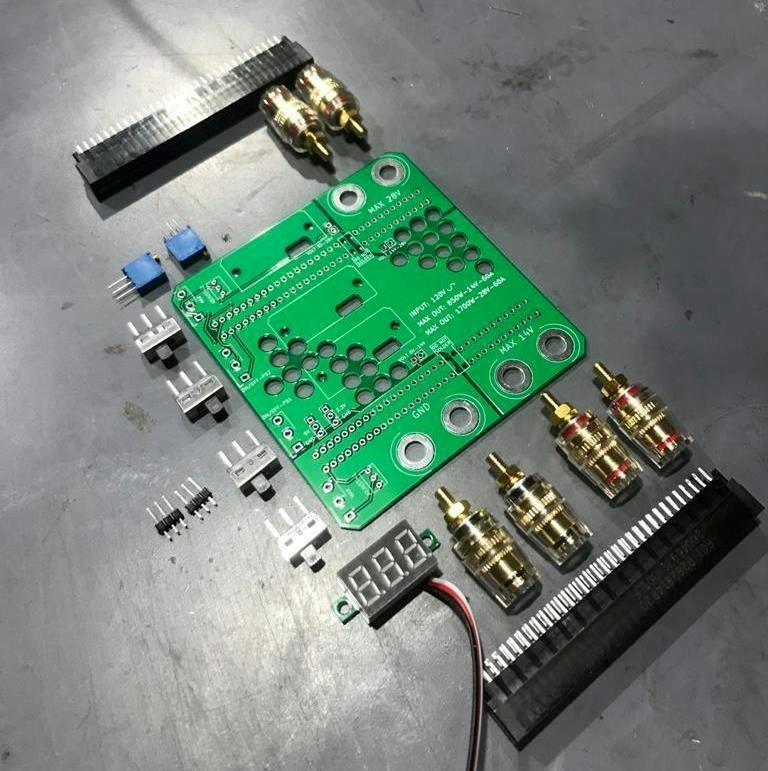
\includegraphics[width=443.6pt,height=445.21pt]{latexImage_d841c33abcd18403b74761391eb9cf3d.png}}
\put(69.384,-72.44){\fontsize{12}{1}\usefont{T1}{ptm}{m}{n}\selectfont\color{color_29791}子之一是亞馬遜包裝系}
\put(190.464,-72.44){\fontsize{12}{1}\usefont{T1}{ptm}{m}{n}\selectfont\color{color_29791}統。例如,買家收到來}
\put(311.544,-72.44){\fontsize{12}{1}\usefont{T1}{ptm}{m}{n}\selectfont\color{color_29791}自亞馬遜的包裹,其中}
\put(432.624,-72.44){\fontsize{12}{1}\usefont{T1}{ptm}{m}{n}\selectfont\color{color_29791}包含根據其}
\put(493.104,-72.44){\fontsize{12}{1}\usefont{T1}{ptm}{m}{n}\selectfont\color{color_29791}特}
\put(69.384,-90.34003){\fontsize{12}{1}\usefont{T1}{ptm}{m}{n}\selectfont\color{color_29791}定訂單專門為他}
\put(153.38,-90.34003){\fontsize{12}{1}\usefont{T1}{ptm}{m}{n}\selectfont\color{color_29791}/}
\put(156.74,-90.34003){\fontsize{12}{1}\usefont{T1}{ptm}{m}{n}\selectfont\color{color_29791}她包}
\put(180.848,-90.34003){\fontsize{12}{1}\usefont{T1}{ptm}{m}{n}\selectfont\color{color_29791}裝的混合產品。雖然本}
\put(300.956,-90.34003){\fontsize{12}{1}\usefont{T1}{ptm}{m}{n}\selectfont\color{color_29791}質上是膚淺的,但這代}
\put(421.064,-90.34003){\fontsize{12}{1}\usefont{T1}{ptm}{m}{n}\selectfont\color{color_29791}表了對客戶的}
\put(492.944,-90.34003){\fontsize{12}{1}\usefont{T1}{ptm}{m}{n}\selectfont\color{color_29791}高}
\put(69.384,-108.34){\fontsize{12}{1}\usefont{T1}{ptm}{m}{n}\selectfont\color{color_29791}度定製。}
\put(116.54,-108.34){\fontsize{12}{1}\usefont{T1}{ptm}{m}{n}\selectfont\color{color_29791} }
\put(63.024,-126.46){\fontsize{12}{1}\usefont{T1}{ptm}{m}{n}\selectfont\color{color_29791} }
\put(82.944,-142.06){\fontsize{12}{1}\usefont{T1}{ptm}{m}{n}\selectfont\color{color_29791}另一}
\put(107.052,-142.06){\fontsize{12}{1}\usefont{T1}{ptm}{m}{n}\selectfont\color{color_29791}個很}
\put(131.16,-142.06){\fontsize{12}{1}\usefont{T1}{ptm}{m}{n}\selectfont\color{color_29791}好的}
\put(155.268,-142.06){\fontsize{12}{1}\usefont{T1}{ptm}{m}{n}\selectfont\color{color_29791}例子}
\put(179.376,-142.06){\fontsize{12}{1}\usefont{T1}{ptm}{m}{n}\selectfont\color{color_29791}是電}
\put(203.484,-142.06){\fontsize{12}{1}\usefont{T1}{ptm}{m}{n}\selectfont\color{color_29791}子原}
\put(227.592,-142.06){\fontsize{12}{1}\usefont{T1}{ptm}{m}{n}\selectfont\color{color_29791}型設}
\put(251.7,-142.06){\fontsize{12}{1}\usefont{T1}{ptm}{m}{n}\selectfont\color{color_29791}計。}
\put(275.808,-142.06){\fontsize{12}{1}\usefont{T1}{ptm}{m}{n}\selectfont\color{color_29791}目前}
\put(299.916,-142.06){\fontsize{12}{1}\usefont{T1}{ptm}{m}{n}\selectfont\color{color_29791},有}
\put(324.024,-142.06){\fontsize{12}{1}\usefont{T1}{ptm}{m}{n}\selectfont\color{color_29791}些公}
\put(348.132,-142.06){\fontsize{12}{1}\usefont{T1}{ptm}{m}{n}\selectfont\color{color_29791}司採}
\put(372.24,-142.06){\fontsize{12}{1}\usefont{T1}{ptm}{m}{n}\selectfont\color{color_29791}用您}
\put(396.348,-142.06){\fontsize{12}{1}\usefont{T1}{ptm}{m}{n}\selectfont\color{color_29791}的印}
\put(420.456,-142.06){\fontsize{12}{1}\usefont{T1}{ptm}{m}{n}\selectfont\color{color_29791}刷電}
\put(444.564,-142.06){\fontsize{12}{1}\usefont{T1}{ptm}{m}{n}\selectfont\color{color_29791}路板}
\put(468.672,-142.06){\fontsize{12}{1}\usefont{T1}{ptm}{m}{n}\selectfont\color{color_29791}設計和}
\put(504.94,-142.06){\fontsize{12}{1}\usefont{T1}{ptm}{m}{n}\selectfont\color{color_29791} }
\put(69.384,-159.94){\fontsize{12}{1}\usefont{T1}{ptm}{m}{n}\selectfont\color{color_29791}B}
\put(77.304,-159.94){\fontsize{12}{1}\usefont{T1}{ptm}{m}{n}\selectfont\color{color_29791}O}
\put(85.82401,-159.94){\fontsize{12}{1}\usefont{T1}{ptm}{m}{n}\selectfont\color{color_29791}M}
\put(96.5,-159.94){\fontsize{12}{1}\usefont{T1}{ptm}{m}{n}\selectfont\color{color_29791},以低成本提供}
\put(180.608,-159.94){\fontsize{12}{1}\usefont{T1}{ptm}{m}{n}\selectfont\color{color_29791}小批量組裝的原型。電}
\put(300.716,-159.94){\fontsize{12}{1}\usefont{T1}{ptm}{m}{n}\selectfont\color{color_29791}子設備的原型製作曾經}
\put(420.824,-159.94){\fontsize{12}{1}\usefont{T1}{ptm}{m}{n}\selectfont\color{color_29791}是一個非常昂貴}
\put(69.384,-177.82){\fontsize{12}{1}\usefont{T1}{ptm}{m}{n}\selectfont\color{color_29791}的過程,但一些公}
\put(164.532,-177.82){\fontsize{12}{1}\usefont{T1}{ptm}{m}{n}\selectfont\color{color_29791}司已}
\put(188.4,-177.82){\fontsize{12}{1}\usefont{T1}{ptm}{m}{n}\selectfont\color{color_29791}經將他們的生產靈}
\put(283.548,-177.82){\fontsize{12}{1}\usefont{T1}{ptm}{m}{n}\selectfont\color{color_29791}活化}
\put(307.416,-177.82){\fontsize{12}{1}\usefont{T1}{ptm}{m}{n}\selectfont\color{color_29791}到能夠快速可靠地}
\put(402.564,-177.82){\fontsize{12}{1}\usefont{T1}{ptm}{m}{n}\selectfont\color{color_29791}交付}
\put(426.432,-177.82){\fontsize{12}{1}\usefont{T1}{ptm}{m}{n}\selectfont\color{color_29791}的程度。同樣}
\put(497.98,-177.82){\fontsize{12}{1}\usefont{T1}{ptm}{m}{n}\selectfont\color{color_29791} }
\put(69.384,-195.7){\fontsize{12}{1}\usefont{T1}{ptm}{m}{n}\selectfont\color{color_29791},這是可能的,因}
\put(164.532,-195.7){\fontsize{12}{1}\usefont{T1}{ptm}{m}{n}\selectfont\color{color_29791}為電}
\put(188.4,-195.7){\fontsize{12}{1}\usefont{T1}{ptm}{m}{n}\selectfont\color{color_29791}子元件本質上是模}
\put(283.548,-195.7){\fontsize{12}{1}\usefont{T1}{ptm}{m}{n}\selectfont\color{color_29791}組化}
\put(307.416,-195.7){\fontsize{12}{1}\usefont{T1}{ptm}{m}{n}\selectfont\color{color_29791}系統,即使複雜性}
\put(402.564,-195.7){\fontsize{12}{1}\usefont{T1}{ptm}{m}{n}\selectfont\color{color_29791}很高}
\put(426.432,-195.7){\fontsize{12}{1}\usefont{T1}{ptm}{m}{n}\selectfont\color{color_29791}。下圖(圖}
\put(485.98,-195.7){\fontsize{12}{1}\usefont{T1}{ptm}{m}{n}\selectfont\color{color_29791}6}
\put(491.86,-195.7){\fontsize{12}{1}\usefont{T1}{ptm}{m}{n}\selectfont\color{color_29791}:}
\put(503.86,-195.7){\fontsize{15}{1}\usefont{T1}{ptm}{m}{n}\selectfont\color{color_29791} }
\put(69.384,-213.58){\fontsize{12}{1}\usefont{T1}{ptm}{m}{n}\selectfont\color{color_29791}電源適配器電路示}
\put(164.532,-213.58){\fontsize{12}{1}\usefont{T1}{ptm}{m}{n}\selectfont\color{color_29791}例專}
\put(188.4,-213.58){\fontsize{12}{1}\usefont{T1}{ptm}{m}{n}\selectfont\color{color_29791}案)是該學生在一}
\put(283.548,-213.58){\fontsize{12}{1}\usefont{T1}{ptm}{m}{n}\selectfont\color{color_29791}周內}
\put(307.416,-213.58){\fontsize{12}{1}\usefont{T1}{ptm}{m}{n}\selectfont\color{color_29791}設計並由}
\put(355.03,-213.58){\fontsize{12}{1}\usefont{T1}{ptm}{m}{n}\selectfont\color{color_29791}J}
\put(359.59,-213.58){\fontsize{12}{1}\usefont{T1}{ptm}{m}{n}\selectfont\color{color_29791}L}
\put(366.79,-213.58){\fontsize{12}{1}\usefont{T1}{ptm}{m}{n}\selectfont\color{color_29791}C}
\put(374.71,-213.58){\fontsize{12}{1}\usefont{T1}{ptm}{m}{n}\selectfont\color{color_29791}P}
\put(381.31,-213.58){\fontsize{12}{1}\usefont{T1}{ptm}{m}{n}\selectfont\color{color_29791}C}
\put(389.23,-213.58){\fontsize{12}{1}\usefont{T1}{ptm}{m}{n}\selectfont\color{color_29791}B}
\put(397.15,-213.58){\fontsize{12}{1}\usefont{T1}{ptm}{m}{n}\selectfont\color{color_29791}製}
\put(409.03,-213.58){\fontsize{12}{1}\usefont{T1}{ptm}{m}{n}\selectfont\color{color_29791}造的}
\put(432.91,-213.58){\fontsize{12}{1}\usefont{T1}{ptm}{m}{n}\selectfont\color{color_29791}電}
\put(444.79,-213.58){\fontsize{12}{1}\usefont{T1}{ptm}{m}{n}\selectfont\color{color_29791}子}
\put(456.67,-213.58){\fontsize{12}{1}\usefont{T1}{ptm}{m}{n}\selectfont\color{color_29791}電}
\put(468.55,-213.58){\fontsize{12}{1}\usefont{T1}{ptm}{m}{n}\selectfont\color{color_29791}路}
\put(480.43,-213.58){\fontsize{12}{1}\usefont{T1}{ptm}{m}{n}\selectfont\color{color_29791}示}
\put(492.31,-213.58){\fontsize{12}{1}\usefont{T1}{ptm}{m}{n}\selectfont\color{color_29791}例}
\put(504.19,-213.58){\fontsize{12}{1}\usefont{T1}{ptm}{m}{n}\selectfont\color{color_29791}。}
\put(516.22,-213.58){\fontsize{12}{1}\usefont{T1}{ptm}{m}{n}\selectfont\color{color_29791} }
\put(63.024,-230.86){\fontsize{9.96}{1}\usefont{T1}{ptm}{m}{n}\selectfont\color{color_29791} }
\put(143.06,-700.496){\fontsize{12}{1}\usefont{T1}{ptm}{b}{n}\selectfont\color{color_29791}圖}
\put(155.06,-700.496){\fontsize{12}{1}\usefont{T1}{ptm}{b}{n}\selectfont\color{color_29791}6}
\put(161.06,-700.496){\fontsize{12}{1}\usefont{T1}{ptm}{b}{n}\selectfont\color{color_29791}電源配}
\put(196.94,-700.496){\fontsize{12}{1}\usefont{T1}{ptm}{b}{n}\selectfont\color{color_29791}接器電}
\put(232.82,-700.496){\fontsize{12}{1}\usefont{T1}{ptm}{b}{n}\selectfont\color{color_29791}路示}
\put(256.7,-700.496){\fontsize{12}{1}\usefont{T1}{ptm}{b}{n}\selectfont\color{color_29791}例專案}
\put(292.61,-700.496){\fontsize{12}{1}\usefont{T1}{ptm}{b}{n}\selectfont\color{color_29791} }
\end{picture}
\newpage
\begin{tikzpicture}[overlay]\path(0pt,0pt);\end{tikzpicture}
\begin{picture}(-5,0)(2.5,0)
\put(500.26,-727.616){\fontsize{12}{1}\usefont{T1}{ptm}{m}{n}\selectfont\color{color_29791}12}
\put(511.78,-727.616){\fontsize{12}{1}\usefont{T1}{ptm}{m}{n}\selectfont\color{color_29791} }
\put(63.024,-726.896){\fontsize{9.96}{1}\usefont{T1}{ptm}{m}{n}\selectfont\color{color_29791} }
\put(200.1,-673.75){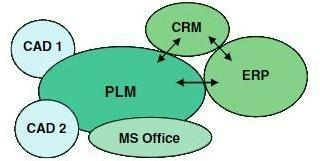
\includegraphics[width=189.47pt,height=95.35001pt]{latexImage_5df76bd8378db0199ccc37b67968bb44.png}}
\put(82.944,-87.34003){\fontsize{12}{1}\usefont{T1}{ptm}{m}{n}\selectfont\color{color_29791}總而言之,其結果再次是對變革的控制和管理的更大需求。這意味著}
\put(443.02,-87.34003){\fontsize{12}{1}\usefont{T1}{ptm}{m}{n}\selectfont\color{color_29791}P}
\put(449.5,-87.34003){\fontsize{12}{1}\usefont{T1}{ptm}{m}{n}\selectfont\color{color_29791}L}
\put(456.58,-87.34003){\fontsize{12}{1}\usefont{T1}{ptm}{m}{n}\selectfont\color{color_29791}M}
\put(467.02,-87.34003){\fontsize{12}{1}\usefont{T1}{ptm}{m}{n}\selectfont\color{color_29791}-}
\put(470.86,-87.34003){\fontsize{12}{1}\usefont{T1}{ptm}{m}{n}\selectfont\color{color_29791} }
\put(69.384,-105.22){\fontsize{12}{1}\usefont{T1}{ptm}{m}{n}\selectfont\color{color_29791}M}
\put(79.944,-105.22){\fontsize{12}{1}\usefont{T1}{ptm}{m}{n}\selectfont\color{color_29791}E}
\put(87.144,-105.22){\fontsize{12}{1}\usefont{T1}{ptm}{m}{n}\selectfont\color{color_29791}S}
\put(93.86,-105.22){\fontsize{12}{1}\usefont{T1}{ptm}{m}{n}\selectfont\color{color_29791}系統的實施將}
\put(165.968,-105.22){\fontsize{12}{1}\usefont{T1}{ptm}{m}{n}\selectfont\color{color_29791}有很}
\put(190.076,-105.22){\fontsize{12}{1}\usefont{T1}{ptm}{m}{n}\selectfont\color{color_29791}大説明。}
\put(238.13,-105.22){\fontsize{12}{1}\usefont{T1}{ptm}{m}{n}\selectfont\color{color_29791}P}
\put(244.73,-105.22){\fontsize{12}{1}\usefont{T1}{ptm}{m}{n}\selectfont\color{color_29791}L}
\put(251.93,-105.22){\fontsize{12}{1}\usefont{T1}{ptm}{m}{n}\selectfont\color{color_29791}M}
\put(262.61,-105.22){\fontsize{12}{1}\usefont{T1}{ptm}{m}{n}\selectfont\color{color_29791}將需}
\put(286.718,-105.22){\fontsize{12}{1}\usefont{T1}{ptm}{m}{n}\selectfont\color{color_29791}要在}
\put(310.826,-105.22){\fontsize{12}{1}\usefont{T1}{ptm}{m}{n}\selectfont\color{color_29791}小批量產品的整}
\put(394.934,-105.22){\fontsize{12}{1}\usefont{T1}{ptm}{m}{n}\selectfont\color{color_29791}個生命}
\put(431.042,-105.22){\fontsize{12}{1}\usefont{T1}{ptm}{m}{n}\selectfont\color{color_29791}週期中管理變}
\put(69.384,-123.1){\fontsize{12}{1}\usefont{T1}{ptm}{m}{n}\selectfont\color{color_29791}化和創新}
\put(117.492,-123.1){\fontsize{12}{1}\usefont{T1}{ptm}{m}{n}\selectfont\color{color_29791},而}
\put(141.5,-123.1){\fontsize{12}{1}\usefont{T1}{ptm}{m}{n}\selectfont\color{color_29791}M}
\put(152.06,-123.1){\fontsize{12}{1}\usefont{T1}{ptm}{m}{n}\selectfont\color{color_29791}E}
\put(159.26,-123.1){\fontsize{12}{1}\usefont{T1}{ptm}{m}{n}\selectfont\color{color_29791}S}
\put(165.98,-123.1){\fontsize{12}{1}\usefont{T1}{ptm}{m}{n}\selectfont\color{color_29791}將}
\put(178.088,-123.1){\fontsize{12}{1}\usefont{T1}{ptm}{m}{n}\selectfont\color{color_29791}提}
\put(190.196,-123.1){\fontsize{12}{1}\usefont{T1}{ptm}{m}{n}\selectfont\color{color_29791}供必要的}
\put(238.304,-123.1){\fontsize{12}{1}\usefont{T1}{ptm}{m}{n}\selectfont\color{color_29791}即時反應}
\put(286.412,-123.1){\fontsize{12}{1}\usefont{T1}{ptm}{m}{n}\selectfont\color{color_29791}和反}
\put(310.52,-123.1){\fontsize{12}{1}\usefont{T1}{ptm}{m}{n}\selectfont\color{color_29791}饋,以減}
\put(358.628,-123.1){\fontsize{12}{1}\usefont{T1}{ptm}{m}{n}\selectfont\color{color_29791}少可能導}
\put(406.736,-123.1){\fontsize{12}{1}\usefont{T1}{ptm}{m}{n}\selectfont\color{color_29791}致整}
\put(430.844,-123.1){\fontsize{12}{1}\usefont{T1}{ptm}{m}{n}\selectfont\color{color_29791}個批次丟}
\put(478.952,-123.1){\fontsize{12}{1}\usefont{T1}{ptm}{m}{n}\selectfont\color{color_29791}失的}
\put(69.384,-140.98){\fontsize{12}{1}\usefont{T1}{ptm}{m}{n}\selectfont\color{color_29791}錯誤。}
\put(104.78,-140.98){\fontsize{12}{1}\usefont{T1}{ptm}{m}{n}\selectfont\color{color_29791} }
\put(63.024,-158.86){\fontsize{12}{1}\usefont{T1}{ptm}{m}{n}\selectfont\color{color_29791} }
\put(63.024,-189.46){\fontsize{12}{1}\usefont{T1}{ptm}{m}{n}\selectfont\color{color_29791} }
\put(265.73,-213.22){\fontsize{15.82003}{1}\usefont{T1}{ptm}{b}{n}\selectfont\color{color_29791}3.}
\put(277.61,-213.22){\fontsize{15.83535}{1}\usefont{T1}{ptm}{b}{n}\selectfont\color{color_29791} }
\put(281.57,-213.22){\fontsize{15.96}{1}\usefont{T1}{ptm}{b}{n}\selectfont\color{color_29791}章節}
\put(313.03,-213.22){\fontsize{15.96}{1}\usefont{T1}{ptm}{b}{n}\selectfont\color{color_29791} }
\put(90.98,-253.21){\fontsize{15.96}{1}\usefont{T1}{ptm}{b}{n}\selectfont\color{color_29791}PLM}
\put(126.5,-253.21){\fontsize{15.96}{1}\usefont{T1}{ptm}{b}{n}\selectfont\color{color_29791} }
\put(129.86,-253.21){\fontsize{15.96}{1}\usefont{T1}{ptm}{b}{n}\selectfont\color{color_29791}和}
\put(145.7,-253.21){\fontsize{15.96}{1}\usefont{T1}{ptm}{b}{n}\selectfont\color{color_29791} }
\put(149.42,-253.21){\fontsize{15.96}{1}\usefont{T1}{ptm}{b}{n}\selectfont\color{color_29791}M}
\put(164.5182,-253.21){\fontsize{15.96}{1}\usefont{T1}{ptm}{b}{n}\selectfont\color{color_29791}ES}
\put(184.13,-253.21){\fontsize{15.96}{1}\usefont{T1}{ptm}{b}{n}\selectfont\color{color_29791} }
\put(187.61,-253.21){\fontsize{15.96}{1}\usefont{T1}{ptm}{b}{n}\selectfont\color{color_29791}的最}
\put(219.4023,-253.21){\fontsize{15.96}{1}\usefont{T1}{ptm}{b}{n}\selectfont\color{color_29791}新技}
\put(251.1946,-253.21){\fontsize{15.96}{1}\usefont{T1}{ptm}{b}{n}\selectfont\color{color_29791}術與}
\put(282.987,-253.21){\fontsize{15.96}{1}\usefont{T1}{ptm}{b}{n}\selectfont\color{color_29791}整合}
\put(314.95,-253.21){\fontsize{15.96}{1}\usefont{T1}{ptm}{b}{n}\selectfont\color{color_29791} }
\put(69.384,-286.81){\fontsize{12}{1}\usefont{T1}{ptm}{m}{n}\selectfont\color{color_29791}不幸的是,關於}
\put(152.54,-286.81){\fontsize{12}{1}\usefont{T1}{ptm}{m}{n}\selectfont\color{color_29791}P}
\put(159.14,-286.81){\fontsize{12}{1}\usefont{T1}{ptm}{m}{n}\selectfont\color{color_29791}L}
\put(166.34,-286.81){\fontsize{12}{1}\usefont{T1}{ptm}{m}{n}\selectfont\color{color_29791}M}
\put(177.02,-286.81){\fontsize{12}{1}\usefont{T1}{ptm}{m}{n}\selectfont\color{color_29791}和}
\put(189.05,-286.81){\fontsize{12}{1}\usefont{T1}{ptm}{m}{n}\selectfont\color{color_29791}M}
\put(199.61,-286.81){\fontsize{12}{1}\usefont{T1}{ptm}{m}{n}\selectfont\color{color_29791}E}
\put(206.81,-286.81){\fontsize{12}{1}\usefont{T1}{ptm}{m}{n}\selectfont\color{color_29791}S}
\put(213.41,-286.81){\fontsize{12}{1}\usefont{T1}{ptm}{m}{n}\selectfont\color{color_29791}系}
\put(225.29,-286.81){\fontsize{12}{1}\usefont{T1}{ptm}{m}{n}\selectfont\color{color_29791}統}
\put(237.17,-286.81){\fontsize{12}{1}\usefont{T1}{ptm}{m}{n}\selectfont\color{color_29791}之}
\put(249.05,-286.81){\fontsize{12}{1}\usefont{T1}{ptm}{m}{n}\selectfont\color{color_29791}間}
\put(260.93,-286.81){\fontsize{12}{1}\usefont{T1}{ptm}{m}{n}\selectfont\color{color_29791}集}
\put(272.81,-286.81){\fontsize{12}{1}\usefont{T1}{ptm}{m}{n}\selectfont\color{color_29791}成}
\put(284.69,-286.81){\fontsize{12}{1}\usefont{T1}{ptm}{m}{n}\selectfont\color{color_29791}的研究}
\put(320.57,-286.81){\fontsize{12}{1}\usefont{T1}{ptm}{m}{n}\selectfont\color{color_29791}並}
\put(332.45,-286.81){\fontsize{12}{1}\usefont{T1}{ptm}{m}{n}\selectfont\color{color_29791}不}
\put(344.33,-286.81){\fontsize{12}{1}\usefont{T1}{ptm}{m}{n}\selectfont\color{color_29791}多}
\put(356.2101,-286.81){\fontsize{12}{1}\usefont{T1}{ptm}{m}{n}\selectfont\color{color_29791}。}
\put(368.0901,-286.81){\fontsize{12}{1}\usefont{T1}{ptm}{m}{n}\selectfont\color{color_29791}但}
\put(379.9701,-286.81){\fontsize{12}{1}\usefont{T1}{ptm}{m}{n}\selectfont\color{color_29791}是}
\put(391.8501,-286.81){\fontsize{12}{1}\usefont{T1}{ptm}{m}{n}\selectfont\color{color_29791},對}
\put(415.7301,-286.81){\fontsize{12}{1}\usefont{T1}{ptm}{m}{n}\selectfont\color{color_29791}於上}
\put(439.6101,-286.81){\fontsize{12}{1}\usefont{T1}{ptm}{m}{n}\selectfont\color{color_29791}述}
\put(451.4901,-286.81){\fontsize{12}{1}\usefont{T1}{ptm}{m}{n}\selectfont\color{color_29791}整}
\put(463.3701,-286.81){\fontsize{12}{1}\usefont{T1}{ptm}{m}{n}\selectfont\color{color_29791}合}
\put(475.2501,-286.81){\fontsize{12}{1}\usefont{T1}{ptm}{m}{n}\selectfont\color{color_29791}的}
\put(487.1301,-286.81){\fontsize{12}{1}\usefont{T1}{ptm}{m}{n}\selectfont\color{color_29791}最}
\put(69.384,-304.81){\fontsize{12}{1}\usefont{T1}{ptm}{m}{n}\selectfont\color{color_29791}可能影響,似乎達}
\put(164.532,-304.81){\fontsize{12}{1}\usefont{T1}{ptm}{m}{n}\selectfont\color{color_29791}成了}
\put(188.4,-304.81){\fontsize{12}{1}\usefont{T1}{ptm}{m}{n}\selectfont\color{color_29791}共識。這些是同步}
\put(283.548,-304.81){\fontsize{12}{1}\usefont{T1}{ptm}{m}{n}\selectfont\color{color_29791}和更}
\put(307.416,-304.81){\fontsize{12}{1}\usefont{T1}{ptm}{m}{n}\selectfont\color{color_29791}嚴格的公差。}
\put(378.91,-304.81){\fontsize{12}{1}\usefont{T1}{ptm}{m}{n}\selectfont\color{color_29791} }
\put(63.024,-322.93){\fontsize{12}{1}\usefont{T1}{ptm}{m}{n}\selectfont\color{color_29791} }
\put(69.384,-338.53){\fontsize{12}{1}\usefont{T1}{ptm}{m}{n}\selectfont\color{color_29791}正如}
\put(93.38,-338.53){\fontsize{12}{1}\usefont{T1}{ptm}{m}{n}\selectfont\color{color_29791}D}
\put(101.9,-338.53){\fontsize{12}{1}\usefont{T1}{ptm}{m}{n}\selectfont\color{color_29791}'A}
\put(112.58,-338.53){\fontsize{12}{1}\usefont{T1}{ptm}{m}{n}\selectfont\color{color_29791}n}
\put(118.46,-338.53){\fontsize{12}{1}\usefont{T1}{ptm}{m}{n}\selectfont\color{color_29791}t}
\put(121.7,-338.53){\fontsize{12}{1}\usefont{T1}{ptm}{m}{n}\selectfont\color{color_29791}o}
\put(127.58,-338.53){\fontsize{12}{1}\usefont{T1}{ptm}{m}{n}\selectfont\color{color_29791}n}
\put(133.46,-338.53){\fontsize{12}{1}\usefont{T1}{ptm}{m}{n}\selectfont\color{color_29791}io}
\put(142.82,-338.53){\fontsize{12}{1}\usefont{T1}{ptm}{m}{n}\selectfont\color{color_29791}等人}
\put(166.928,-338.53){\fontsize{12}{1}\usefont{T1}{ptm}{m}{n}\selectfont\color{color_29791}(}
\put(178.94,-338.53){\fontsize{12}{1}\usefont{T1}{ptm}{m}{n}\selectfont\color{color_29791}2}
\put(184.82,-338.53){\fontsize{12}{1}\usefont{T1}{ptm}{m}{n}\selectfont\color{color_29791}01}
\put(196.7,-338.53){\fontsize{12}{1}\usefont{T1}{ptm}{m}{n}\selectfont\color{color_29791}5}
\put(202.73,-338.53){\fontsize{12}{1}\usefont{T1}{ptm}{m}{n}\selectfont\color{color_29791}年)}
\put(226.838,-338.53){\fontsize{12}{1}\usefont{T1}{ptm}{m}{n}\selectfont\color{color_29791}所解釋}
\put(262.946,-338.53){\fontsize{12}{1}\usefont{T1}{ptm}{m}{n}\selectfont\color{color_29791}的那}
\put(287.054,-338.53){\fontsize{12}{1}\usefont{T1}{ptm}{m}{n}\selectfont\color{color_29791}樣,}
\put(311.162,-338.53){\fontsize{12}{1}\usefont{T1}{ptm}{m}{n}\selectfont\color{color_29791}該案例}
\put(347.27,-338.53){\fontsize{12}{1}\usefont{T1}{ptm}{m}{n}\selectfont\color{color_29791}研究側}
\put(383.378,-338.53){\fontsize{12}{1}\usefont{T1}{ptm}{m}{n}\selectfont\color{color_29791}重於涉}
\put(419.486,-338.53){\fontsize{12}{1}\usefont{T1}{ptm}{m}{n}\selectfont\color{color_29791}及}
\put(431.594,-338.53){\fontsize{12}{1}\usefont{T1}{ptm}{m}{n}\selectfont\color{color_29791}航空應}
\put(467.702,-338.53){\fontsize{12}{1}\usefont{T1}{ptm}{m}{n}\selectfont\color{color_29791}用精密}
\put(69.384,-356.41){\fontsize{12}{1}\usefont{T1}{ptm}{m}{n}\selectfont\color{color_29791}部件}
\put(93.492,-356.41){\fontsize{12}{1}\usefont{T1}{ptm}{m}{n}\selectfont\color{color_29791}製造}
\put(117.6,-356.41){\fontsize{12}{1}\usefont{T1}{ptm}{m}{n}\selectfont\color{color_29791}的}
\put(129.708,-356.41){\fontsize{12}{1}\usefont{T1}{ptm}{m}{n}\selectfont\color{color_29791}案例}
\put(153.816,-356.41){\fontsize{12}{1}\usefont{T1}{ptm}{m}{n}\selectfont\color{color_29791}研究}
\put(177.924,-356.41){\fontsize{12}{1}\usefont{T1}{ptm}{m}{n}\selectfont\color{color_29791},}
\put(190.032,-356.41){\fontsize{12}{1}\usefont{T1}{ptm}{m}{n}\selectfont\color{color_29791}部署}
\put(214.14,-356.41){\fontsize{12}{1}\usefont{T1}{ptm}{m}{n}\selectfont\color{color_29791}監測}
\put(238.248,-356.41){\fontsize{12}{1}\usefont{T1}{ptm}{m}{n}\selectfont\color{color_29791}和}
\put(250.356,-356.41){\fontsize{12}{1}\usefont{T1}{ptm}{m}{n}\selectfont\color{color_29791}控制}
\put(274.464,-356.41){\fontsize{12}{1}\usefont{T1}{ptm}{m}{n}\selectfont\color{color_29791}系統}
\put(298.572,-356.41){\fontsize{12}{1}\usefont{T1}{ptm}{m}{n}\selectfont\color{color_29791}的}
\put(310.68,-356.41){\fontsize{12}{1}\usefont{T1}{ptm}{m}{n}\selectfont\color{color_29791}第一}
\put(334.788,-356.41){\fontsize{12}{1}\usefont{T1}{ptm}{m}{n}\selectfont\color{color_29791}個優}
\put(358.896,-356.41){\fontsize{12}{1}\usefont{T1}{ptm}{m}{n}\selectfont\color{color_29791}勢}
\put(371.004,-356.41){\fontsize{12}{1}\usefont{T1}{ptm}{m}{n}\selectfont\color{color_29791}是產}
\put(395.112,-356.41){\fontsize{12}{1}\usefont{T1}{ptm}{m}{n}\selectfont\color{color_29791}品品}
\put(419.22,-356.41){\fontsize{12}{1}\usefont{T1}{ptm}{m}{n}\selectfont\color{color_29791}質}
\put(431.328,-356.41){\fontsize{12}{1}\usefont{T1}{ptm}{m}{n}\selectfont\color{color_29791}的提}
\put(455.436,-356.41){\fontsize{12}{1}\usefont{T1}{ptm}{m}{n}\selectfont\color{color_29791}高:}
\put(479.544,-356.41){\fontsize{12}{1}\usefont{T1}{ptm}{m}{n}\selectfont\color{color_29791}感測}
\put(69.384,-374.29){\fontsize{12}{1}\usefont{T1}{ptm}{m}{n}\selectfont\color{color_29791}器允許檢測,測量}
\put(164.532,-374.29){\fontsize{12}{1}\usefont{T1}{ptm}{m}{n}\selectfont\color{color_29791}和監}
\put(188.4,-374.29){\fontsize{12}{1}\usefont{T1}{ptm}{m}{n}\selectfont\color{color_29791}測影響過程性能或}
\put(283.548,-374.29){\fontsize{12}{1}\usefont{T1}{ptm}{m}{n}\selectfont\color{color_29791}產品}
\put(307.416,-374.29){\fontsize{12}{1}\usefont{T1}{ptm}{m}{n}\selectfont\color{color_29791}品質的變數,事件}
\put(402.564,-374.29){\fontsize{12}{1}\usefont{T1}{ptm}{m}{n}\selectfont\color{color_29791}和情}
\put(426.432,-374.29){\fontsize{12}{1}\usefont{T1}{ptm}{m}{n}\selectfont\color{color_29791}況。}
\put(450.34,-374.29){\fontsize{12}{1}\usefont{T1}{ptm}{m}{n}\selectfont\color{color_29791} }
\put(63.024,-392.53){\fontsize{12}{1}\usefont{T1}{ptm}{m}{n}\selectfont\color{color_29791} }
\put(82.944,-408.13){\fontsize{12}{1}\usefont{T1}{ptm}{m}{n}\selectfont\color{color_29791}將}
\put(94.46,-408.13){\fontsize{12}{1}\usefont{T1}{ptm}{m}{n}\selectfont\color{color_29791} }
\put(487.9,-408.13){\fontsize{12}{1}\usefont{T1}{ptm}{m}{n}\selectfont\color{color_29791}P}
\put(494.38,-408.13){\fontsize{12}{1}\usefont{T1}{ptm}{m}{n}\selectfont\color{color_29791}L}
\put(501.46,-408.13){\fontsize{12}{1}\usefont{T1}{ptm}{m}{n}\selectfont\color{color_29791}M}
\put(511.78,-408.13){\fontsize{12}{1}\usefont{T1}{ptm}{m}{n}\selectfont\color{color_29791} }
\put(69.384,-426.03){\fontsize{12}{1}\usefont{T1}{ptm}{m}{n}\selectfont\color{color_29791}與任何其他系統整合的}
\put(190.464,-426.03){\fontsize{12}{1}\usefont{T1}{ptm}{m}{n}\selectfont\color{color_29791}核心問題之一圍繞著資}
\put(311.544,-426.03){\fontsize{12}{1}\usefont{T1}{ptm}{m}{n}\selectfont\color{color_29791}訊的擁有權。一個可能}
\put(432.624,-426.03){\fontsize{12}{1}\usefont{T1}{ptm}{m}{n}\selectfont\color{color_29791}的解決方案依}
\put(69.384,-444.03){\fontsize{12}{1}\usefont{T1}{ptm}{m}{n}\selectfont\color{color_29791}賴於}
\put(93.492,-444.03){\fontsize{12}{1}\usefont{T1}{ptm}{m}{n}\selectfont\color{color_29791}資}
\put(105.6,-444.03){\fontsize{12}{1}\usefont{T1}{ptm}{m}{n}\selectfont\color{color_29791}料庫}
\put(129.708,-444.03){\fontsize{12}{1}\usefont{T1}{ptm}{m}{n}\selectfont\color{color_29791}集}
\put(141.816,-444.03){\fontsize{12}{1}\usefont{T1}{ptm}{m}{n}\selectfont\color{color_29791}成以}
\put(165.924,-444.03){\fontsize{12}{1}\usefont{T1}{ptm}{m}{n}\selectfont\color{color_29791}及}
\put(178.032,-444.03){\fontsize{12}{1}\usefont{T1}{ptm}{m}{n}\selectfont\color{color_29791}系}
\put(190.14,-444.03){\fontsize{12}{1}\usefont{T1}{ptm}{m}{n}\selectfont\color{color_29791}統之}
\put(214.248,-444.03){\fontsize{12}{1}\usefont{T1}{ptm}{m}{n}\selectfont\color{color_29791}間}
\put(226.356,-444.03){\fontsize{12}{1}\usefont{T1}{ptm}{m}{n}\selectfont\color{color_29791}的中}
\put(250.464,-444.03){\fontsize{12}{1}\usefont{T1}{ptm}{m}{n}\selectfont\color{color_29791}間}
\put(262.572,-444.03){\fontsize{12}{1}\usefont{T1}{ptm}{m}{n}\selectfont\color{color_29791}件的}
\put(286.68,-444.03){\fontsize{12}{1}\usefont{T1}{ptm}{m}{n}\selectfont\color{color_29791}使}
\put(298.788,-444.03){\fontsize{12}{1}\usefont{T1}{ptm}{m}{n}\selectfont\color{color_29791}用}
\put(310.896,-444.03){\fontsize{12}{1}\usefont{T1}{ptm}{m}{n}\selectfont\color{color_29791}。正}
\put(335.004,-444.03){\fontsize{12}{1}\usefont{T1}{ptm}{m}{n}\selectfont\color{color_29791}如}
\put(347.23,-444.03){\fontsize{12}{1}\usefont{T1}{ptm}{m}{n}\selectfont\color{color_29791}S}
\put(353.83,-444.03){\fontsize{12}{1}\usefont{T1}{ptm}{m}{n}\selectfont\color{color_29791}a}
\put(359.11,-444.03){\fontsize{12}{1}\usefont{T1}{ptm}{m}{n}\selectfont\color{color_29791}a}
\put(364.27,-444.03){\fontsize{12}{1}\usefont{T1}{ptm}{m}{n}\selectfont\color{color_29791}k}
\put(370.15,-444.03){\fontsize{12}{1}\usefont{T1}{ptm}{m}{n}\selectfont\color{color_29791}s}
\put(374.71,-444.03){\fontsize{12}{1}\usefont{T1}{ptm}{m}{n}\selectfont\color{color_29791}v}
\put(380.59,-444.03){\fontsize{12}{1}\usefont{T1}{ptm}{m}{n}\selectfont\color{color_29791}uo}
\put(392.47,-444.03){\fontsize{12}{1}\usefont{T1}{ptm}{m}{n}\selectfont\color{color_29791}ri}
\put(399.79,-444.03){\fontsize{12}{1}\usefont{T1}{ptm}{m}{n}\selectfont\color{color_29791}和}
\put(411.91,-444.03){\fontsize{12}{1}\usefont{T1}{ptm}{m}{n}\selectfont\color{color_29791}I}
\put(415.75,-444.03){\fontsize{12}{1}\usefont{T1}{ptm}{m}{n}\selectfont\color{color_29791}mm}
\put(434.35,-444.03){\fontsize{12}{1}\usefont{T1}{ptm}{m}{n}\selectfont\color{color_29791}o}
\put(440.23,-444.03){\fontsize{12}{1}\usefont{T1}{ptm}{m}{n}\selectfont\color{color_29791}n}
\put(446.11,-444.03){\fontsize{12}{1}\usefont{T1}{ptm}{m}{n}\selectfont\color{color_29791}e}
\put(451.39,-444.03){\fontsize{12}{1}\usefont{T1}{ptm}{m}{n}\selectfont\color{color_29791}n}
\put(457.42,-444.03){\fontsize{12}{1}\usefont{T1}{ptm}{m}{n}\selectfont\color{color_29791}(}
\put(469.42,-444.03){\fontsize{12}{1}\usefont{T1}{ptm}{m}{n}\selectfont\color{color_29791}2}
\put(475.3,-444.03){\fontsize{12}{1}\usefont{T1}{ptm}{m}{n}\selectfont\color{color_29791}00}
\put(487.18,-444.03){\fontsize{12}{1}\usefont{T1}{ptm}{m}{n}\selectfont\color{color_29791}8}
\put(493.18,-444.03){\fontsize{12}{1}\usefont{T1}{ptm}{m}{n}\selectfont\color{color_29791})}
\put(69.384,-462.03){\fontsize{12}{1}\usefont{T1}{ptm}{m}{n}\selectfont\color{color_29791}所寫的那樣。一個合理}
\put(190.464,-462.03){\fontsize{12}{1}\usefont{T1}{ptm}{m}{n}\selectfont\color{color_29791}的目標是資訊應始終在}
\put(311.544,-462.03){\fontsize{12}{1}\usefont{T1}{ptm}{m}{n}\selectfont\color{color_29791}一個地方更新。其他系}
\put(432.624,-462.03){\fontsize{12}{1}\usefont{T1}{ptm}{m}{n}\selectfont\color{color_29791}統可以直接從}
\put(505.06,-462.03){\fontsize{12}{1}\usefont{T1}{ptm}{m}{n}\selectfont\color{color_29791} }
\put(69.384,-479.07){\fontsize{12}{1}\usefont{T1}{ptm}{m}{n}\selectfont\color{color_29791}P}
\put(75.86401,-479.07){\fontsize{12}{1}\usefont{T1}{ptm}{m}{n}\selectfont\color{color_29791}L}
\put(82.94401,-479.07){\fontsize{12}{1}\usefont{T1}{ptm}{m}{n}\selectfont\color{color_29791}M}
\put(93.5,-479.07){\fontsize{12}{1}\usefont{T1}{ptm}{m}{n}\selectfont\color{color_29791} }
\put(69.384,-495.27){\fontsize{12}{1}\usefont{T1}{ptm}{m}{n}\selectfont\color{color_29791}資料庫}
\put(105.264,-495.27){\fontsize{12}{1}\usefont{T1}{ptm}{m}{n}\selectfont\color{color_29791}中讀取}
\put(141.144,-495.27){\fontsize{12}{1}\usefont{T1}{ptm}{m}{n}\selectfont\color{color_29791}資訊}
\put(165.024,-495.27){\fontsize{12}{1}\usefont{T1}{ptm}{m}{n}\selectfont\color{color_29791},如}
\put(188.904,-495.27){\fontsize{12}{1}\usefont{T1}{ptm}{m}{n}\selectfont\color{color_29791}有必要}
\put(224.784,-495.27){\fontsize{12}{1}\usefont{T1}{ptm}{m}{n}\selectfont\color{color_29791},可以}
\put(260.664,-495.27){\fontsize{12}{1}\usefont{T1}{ptm}{m}{n}\selectfont\color{color_29791}在其}
\put(284.544,-495.27){\fontsize{12}{1}\usefont{T1}{ptm}{m}{n}\selectfont\color{color_29791}他系}
\put(308.424,-495.27){\fontsize{12}{1}\usefont{T1}{ptm}{m}{n}\selectfont\color{color_29791}統的資}
\put(344.304,-495.27){\fontsize{12}{1}\usefont{T1}{ptm}{m}{n}\selectfont\color{color_29791}料庫上}
\put(380.1841,-495.27){\fontsize{12}{1}\usefont{T1}{ptm}{m}{n}\selectfont\color{color_29791}複製}
\put(404.0641,-495.27){\fontsize{12}{1}\usefont{T1}{ptm}{m}{n}\selectfont\color{color_29791}所需}
\put(427.9441,-495.27){\fontsize{12}{1}\usefont{T1}{ptm}{m}{n}\selectfont\color{color_29791}的資訊}
\put(463.8241,-495.27){\fontsize{12}{1}\usefont{T1}{ptm}{m}{n}\selectfont\color{color_29791},如圖}
\put(499.78,-495.27){\fontsize{12}{1}\usefont{T1}{ptm}{m}{n}\selectfont\color{color_29791} }
\put(505.78,-495.27){\fontsize{12}{1}\usefont{T1}{ptm}{m}{n}\selectfont\color{color_29791}7}
\put(511.18,-495.27){\fontsize{12}{1}\usefont{T1}{ptm}{m}{n}\selectfont\color{color_29791} }
\put(69.384,-512.43){\fontsize{12}{1}\usefont{T1}{ptm}{m}{n}\selectfont\color{color_29791}所示。雖然它主要}
\put(164.532,-512.43){\fontsize{12}{1}\usefont{T1}{ptm}{m}{n}\selectfont\color{color_29791}從}
\put(176.42,-512.43){\fontsize{12}{1}\usefont{T1}{ptm}{m}{n}\selectfont\color{color_29791}P}
\put(183.02,-512.43){\fontsize{12}{1}\usefont{T1}{ptm}{m}{n}\selectfont\color{color_29791}LM}
\put(200.93,-512.43){\fontsize{12}{1}\usefont{T1}{ptm}{m}{n}\selectfont\color{color_29791}-}
\put(204.77,-512.43){\fontsize{12}{1}\usefont{T1}{ptm}{m}{n}\selectfont\color{color_29791}E}
\put(211.97,-512.43){\fontsize{12}{1}\usefont{T1}{ptm}{m}{n}\selectfont\color{color_29791}R}
\put(219.89,-512.43){\fontsize{12}{1}\usefont{T1}{ptm}{m}{n}\selectfont\color{color_29791}P}
\put(226.49,-512.43){\fontsize{12}{1}\usefont{T1}{ptm}{m}{n}\selectfont\color{color_29791}集}
\put(238.37,-512.43){\fontsize{12}{1}\usefont{T1}{ptm}{m}{n}\selectfont\color{color_29791}成}
\put(250.25,-512.43){\fontsize{12}{1}\usefont{T1}{ptm}{m}{n}\selectfont\color{color_29791}的}
\put(262.13,-512.43){\fontsize{12}{1}\usefont{T1}{ptm}{m}{n}\selectfont\color{color_29791}角}
\put(274.01,-512.43){\fontsize{12}{1}\usefont{T1}{ptm}{m}{n}\selectfont\color{color_29791}度指}
\put(297.89,-512.43){\fontsize{12}{1}\usefont{T1}{ptm}{m}{n}\selectfont\color{color_29791}出了}
\put(321.77,-512.43){\fontsize{12}{1}\usefont{T1}{ptm}{m}{n}\selectfont\color{color_29791}這}
\put(333.65,-512.43){\fontsize{12}{1}\usefont{T1}{ptm}{m}{n}\selectfont\color{color_29791}一}
\put(345.53,-512.43){\fontsize{12}{1}\usefont{T1}{ptm}{m}{n}\selectfont\color{color_29791}點}
\put(357.41,-512.43){\fontsize{12}{1}\usefont{T1}{ptm}{m}{n}\selectfont\color{color_29791},}
\put(369.29,-512.43){\fontsize{12}{1}\usefont{T1}{ptm}{m}{n}\selectfont\color{color_29791}但}
\put(381.17,-512.43){\fontsize{12}{1}\usefont{T1}{ptm}{m}{n}\selectfont\color{color_29791}從}
\put(393.07,-512.43){\fontsize{12}{1}\usefont{T1}{ptm}{m}{n}\selectfont\color{color_29791}P}
\put(399.67,-512.43){\fontsize{12}{1}\usefont{T1}{ptm}{m}{n}\selectfont\color{color_29791}L}
\put(406.75,-512.43){\fontsize{12}{1}\usefont{T1}{ptm}{m}{n}\selectfont\color{color_29791}M}
\put(417.19,-512.43){\fontsize{12}{1}\usefont{T1}{ptm}{m}{n}\selectfont\color{color_29791}-}
\put(421.03,-512.43){\fontsize{12}{1}\usefont{T1}{ptm}{m}{n}\selectfont\color{color_29791} }
\put(69.384,-530.43){\fontsize{12}{1}\usefont{T1}{ptm}{m}{n}\selectfont\color{color_29791}M}
\put(79.944,-530.43){\fontsize{12}{1}\usefont{T1}{ptm}{m}{n}\selectfont\color{color_29791}E}
\put(87.144,-530.43){\fontsize{12}{1}\usefont{T1}{ptm}{m}{n}\selectfont\color{color_29791}S}
\put(93.74,-530.43){\fontsize{12}{1}\usefont{T1}{ptm}{m}{n}\selectfont\color{color_29791}集}
\put(105.62,-530.43){\fontsize{12}{1}\usefont{T1}{ptm}{m}{n}\selectfont\color{color_29791}成}
\put(117.5,-530.43){\fontsize{12}{1}\usefont{T1}{ptm}{m}{n}\selectfont\color{color_29791}的}
\put(129.38,-530.43){\fontsize{12}{1}\usefont{T1}{ptm}{m}{n}\selectfont\color{color_29791}角}
\put(141.26,-530.43){\fontsize{12}{1}\usefont{T1}{ptm}{m}{n}\selectfont\color{color_29791}度}
\put(153.14,-530.43){\fontsize{12}{1}\usefont{T1}{ptm}{m}{n}\selectfont\color{color_29791}來}
\put(165.02,-530.43){\fontsize{12}{1}\usefont{T1}{ptm}{m}{n}\selectfont\color{color_29791}看,它}
\put(200.9,-530.43){\fontsize{12}{1}\usefont{T1}{ptm}{m}{n}\selectfont\color{color_29791}仍}
\put(212.78,-530.43){\fontsize{12}{1}\usefont{T1}{ptm}{m}{n}\selectfont\color{color_29791}然}
\put(224.66,-530.43){\fontsize{12}{1}\usefont{T1}{ptm}{m}{n}\selectfont\color{color_29791}非}
\put(236.54,-530.43){\fontsize{12}{1}\usefont{T1}{ptm}{m}{n}\selectfont\color{color_29791}常}
\put(248.42,-530.43){\fontsize{12}{1}\usefont{T1}{ptm}{m}{n}\selectfont\color{color_29791}有}
\put(260.3,-530.43){\fontsize{12}{1}\usefont{T1}{ptm}{m}{n}\selectfont\color{color_29791}價}
\put(272.1801,-530.43){\fontsize{12}{1}\usefont{T1}{ptm}{m}{n}\selectfont\color{color_29791}值,}
\put(296.0601,-530.43){\fontsize{12}{1}\usefont{T1}{ptm}{m}{n}\selectfont\color{color_29791}因為}
\put(319.9401,-530.43){\fontsize{12}{1}\usefont{T1}{ptm}{m}{n}\selectfont\color{color_29791}它}
\put(331.8201,-530.43){\fontsize{12}{1}\usefont{T1}{ptm}{m}{n}\selectfont\color{color_29791}是}
\put(343.7001,-530.43){\fontsize{12}{1}\usefont{T1}{ptm}{m}{n}\selectfont\color{color_29791}一}
\put(355.5801,-530.43){\fontsize{12}{1}\usefont{T1}{ptm}{m}{n}\selectfont\color{color_29791}個}
\put(367.4601,-530.43){\fontsize{12}{1}\usefont{T1}{ptm}{m}{n}\selectfont\color{color_29791}例}
\put(379.3401,-530.43){\fontsize{12}{1}\usefont{T1}{ptm}{m}{n}\selectfont\color{color_29791}子}
\put(391.2201,-530.43){\fontsize{12}{1}\usefont{T1}{ptm}{m}{n}\selectfont\color{color_29791},說}
\put(415.1001,-530.43){\fontsize{12}{1}\usefont{T1}{ptm}{m}{n}\selectfont\color{color_29791}明如}
\put(438.9801,-530.43){\fontsize{12}{1}\usefont{T1}{ptm}{m}{n}\selectfont\color{color_29791}何}
\put(450.8601,-530.43){\fontsize{12}{1}\usefont{T1}{ptm}{m}{n}\selectfont\color{color_29791}通}
\put(462.7401,-530.43){\fontsize{12}{1}\usefont{T1}{ptm}{m}{n}\selectfont\color{color_29791}過}
\put(474.6201,-530.43){\fontsize{12}{1}\usefont{T1}{ptm}{m}{n}\selectfont\color{color_29791}圍}
\put(486.5001,-530.43){\fontsize{12}{1}\usefont{T1}{ptm}{m}{n}\selectfont\color{color_29791}繞}
\put(69.384,-548.43){\fontsize{12}{1}\usefont{T1}{ptm}{m}{n}\selectfont\color{color_29791}將不同性質的檔載}
\put(164.532,-548.43){\fontsize{12}{1}\usefont{T1}{ptm}{m}{n}\selectfont\color{color_29791}入到}
\put(188.4,-548.43){\fontsize{12}{1}\usefont{T1}{ptm}{m}{n}\selectfont\color{color_29791}集中式}
\put(224.09,-548.43){\fontsize{12}{1}\usefont{T1}{ptm}{m}{n}\selectfont\color{color_29791}P}
\put(230.69,-548.43){\fontsize{12}{1}\usefont{T1}{ptm}{m}{n}\selectfont\color{color_29791}L}
\put(237.89,-548.43){\fontsize{12}{1}\usefont{T1}{ptm}{m}{n}\selectfont\color{color_29791}M}
\put(248.45,-548.43){\fontsize{12}{1}\usefont{T1}{ptm}{m}{n}\selectfont\color{color_29791}-}
\put(252.29,-548.43){\fontsize{12}{1}\usefont{T1}{ptm}{m}{n}\selectfont\color{color_29791}E}
\put(259.49,-548.43){\fontsize{12}{1}\usefont{T1}{ptm}{m}{n}\selectfont\color{color_29791}R}
\put(267.41,-548.43){\fontsize{12}{1}\usefont{T1}{ptm}{m}{n}\selectfont\color{color_29791}P}
\put(274.01,-548.43){\fontsize{12}{1}\usefont{T1}{ptm}{m}{n}\selectfont\color{color_29791}系}
\put(285.89,-548.43){\fontsize{12}{1}\usefont{T1}{ptm}{m}{n}\selectfont\color{color_29791}統中的}
\put(321.77,-548.43){\fontsize{12}{1}\usefont{T1}{ptm}{m}{n}\selectfont\color{color_29791}系}
\put(333.65,-548.43){\fontsize{12}{1}\usefont{T1}{ptm}{m}{n}\selectfont\color{color_29791}統}
\put(345.53,-548.43){\fontsize{12}{1}\usefont{T1}{ptm}{m}{n}\selectfont\color{color_29791}來}
\put(357.41,-548.43){\fontsize{12}{1}\usefont{T1}{ptm}{m}{n}\selectfont\color{color_29791}期}
\put(369.29,-548.43){\fontsize{12}{1}\usefont{T1}{ptm}{m}{n}\selectfont\color{color_29791}望}
\put(381.17,-548.43){\fontsize{12}{1}\usefont{T1}{ptm}{m}{n}\selectfont\color{color_29791}更}
\put(393.05,-548.43){\fontsize{12}{1}\usefont{T1}{ptm}{m}{n}\selectfont\color{color_29791}好的}
\put(416.9301,-548.43){\fontsize{12}{1}\usefont{T1}{ptm}{m}{n}\selectfont\color{color_29791}操作}
\put(440.8101,-548.43){\fontsize{12}{1}\usefont{T1}{ptm}{m}{n}\selectfont\color{color_29791}。}
\put(452.74,-548.43){\fontsize{12}{1}\usefont{T1}{ptm}{m}{n}\selectfont\color{color_29791} }
\put(63.024,-574.59){\fontsize{9.96}{1}\usefont{T1}{ptm}{m}{n}\selectfont\color{color_29791} }
\put(134.78,-703.616){\fontsize{12}{1}\usefont{T1}{ptm}{b}{n}\selectfont\color{color_29791}圖}
\put(146.78,-703.616){\fontsize{12}{1}\usefont{T1}{ptm}{b}{n}\selectfont\color{color_29791} }
\put(149.78,-703.616){\fontsize{12}{1}\usefont{T1}{ptm}{b}{n}\selectfont\color{color_29791}7}
\put(155.78,-703.616){\fontsize{12}{1}\usefont{T1}{ptm}{b}{n}\selectfont\color{color_29791} }
\put(158.78,-703.616){\fontsize{12}{1}\usefont{T1}{ptm}{b}{n}\selectfont\color{color_29791}PLM}
\put(185.45,-703.616){\fontsize{12}{1}\usefont{T1}{ptm}{b}{n}\selectfont\color{color_29791} }
\put(188.33,-703.616){\fontsize{12}{1}\usefont{T1}{ptm}{b}{n}\selectfont\color{color_29791}集成示意圖}
\put(248.21,-703.616){\fontsize{12}{1}\usefont{T1}{ptm}{b}{n}\selectfont\color{color_29791}(}
\put(260.21,-703.616){\fontsize{12}{1}\usefont{T1}{ptm}{b}{n}\selectfont\color{color_29791}S}
\put(266.918,-703.616){\fontsize{12}{1}\usefont{T1}{ptm}{b}{n}\selectfont\color{color_29791}aak}
\put(285.626,-703.616){\fontsize{12}{1}\usefont{T1}{ptm}{b}{n}\selectfont\color{color_29791}svu}
\put(303.014,-703.616){\fontsize{12}{1}\usefont{T1}{ptm}{b}{n}\selectfont\color{color_29791}or}
\put(314.294,-703.616){\fontsize{12}{1}\usefont{T1}{ptm}{b}{n}\selectfont\color{color_29791}i}
\put(317.71,-703.616){\fontsize{12}{1}\usefont{T1}{ptm}{b}{n}\selectfont\color{color_29791} }
\put(320.59,-703.616){\fontsize{12}{1}\usefont{T1}{ptm}{b}{n}\selectfont\color{color_29791}和}
\put(332.59,-703.616){\fontsize{12}{1}\usefont{T1}{ptm}{b}{n}\selectfont\color{color_29791} }
\put(335.59,-703.616){\fontsize{12}{1}\usefont{T1}{ptm}{b}{n}\selectfont\color{color_29791}I}
\put(340.15,-703.616){\fontsize{12}{1}\usefont{T1}{ptm}{b}{n}\selectfont\color{color_29791}m}
\put(350.218,-703.616){\fontsize{12}{1}\usefont{T1}{ptm}{b}{n}\selectfont\color{color_29791}m}
\put(360.286,-703.616){\fontsize{12}{1}\usefont{T1}{ptm}{b}{n}\selectfont\color{color_29791}o}
\put(366.166,-703.616){\fontsize{12}{1}\usefont{T1}{ptm}{b}{n}\selectfont\color{color_29791}n}
\put(372.874,-703.616){\fontsize{12}{1}\usefont{T1}{ptm}{b}{n}\selectfont\color{color_29791}e}
\put(378.154,-703.616){\fontsize{12}{1}\usefont{T1}{ptm}{b}{n}\selectfont\color{color_29791}n}
\put(384.91,-703.616){\fontsize{12}{1}\usefont{T1}{ptm}{b}{n}\selectfont\color{color_29791},}
\put(396.91,-703.616){\fontsize{12}{1}\usefont{T1}{ptm}{b}{n}\selectfont\color{color_29791}2008}
\put(420.91,-703.616){\fontsize{12}{1}\usefont{T1}{ptm}{b}{n}\selectfont\color{color_29791} }
\put(423.79,-703.616){\fontsize{12}{1}\usefont{T1}{ptm}{b}{n}\selectfont\color{color_29791}年}
\put(435.79,-703.616){\fontsize{12}{1}\usefont{T1}{ptm}{b}{n}\selectfont\color{color_29791})}
\put(447.22,-703.616){\fontsize{12}{1}\usefont{T1}{ptm}{b}{n}\selectfont\color{color_29791} }
\end{picture}
\newpage
\begin{tikzpicture}[overlay]\path(0pt,0pt);\end{tikzpicture}
\begin{picture}(-5,0)(2.5,0)
\put(500.26,-727.616){\fontsize{12}{1}\usefont{T1}{ptm}{m}{n}\selectfont\color{color_29791}13}
\put(511.78,-727.616){\fontsize{12}{1}\usefont{T1}{ptm}{m}{n}\selectfont\color{color_29791} }
\put(63.024,-726.896){\fontsize{9.96}{1}\usefont{T1}{ptm}{m}{n}\selectfont\color{color_29791} }
\put(73.05,-615.24){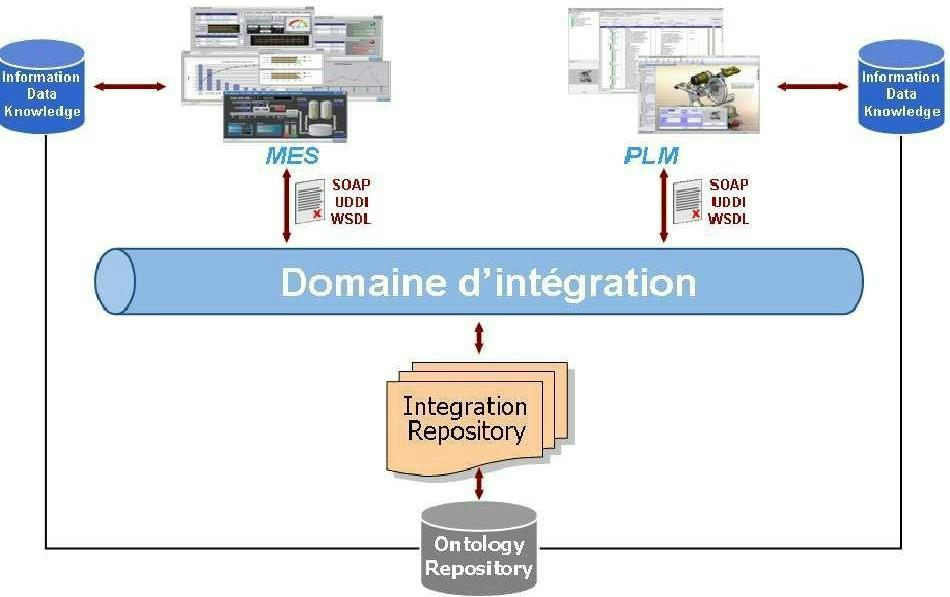
\includegraphics[width=442.1pt,height=277.59pt]{latexImage_b377a07ec99036c9195a01d0980e1175.png}}
\put(69.384,-102.58){\fontsize{12}{1}\usefont{T1}{ptm}{m}{n}\selectfont\color{color_29791}因此,}
\put(105.264,-102.58){\fontsize{12}{1}\usefont{T1}{ptm}{m}{n}\selectfont\color{color_29791}中間件}
\put(141.144,-102.58){\fontsize{12}{1}\usefont{T1}{ptm}{m}{n}\selectfont\color{color_29791}將是}
\put(165.024,-102.58){\fontsize{12}{1}\usefont{T1}{ptm}{m}{n}\selectfont\color{color_29791}一個}
\put(188.904,-102.58){\fontsize{12}{1}\usefont{T1}{ptm}{m}{n}\selectfont\color{color_29791}軟體框}
\put(224.784,-102.58){\fontsize{12}{1}\usefont{T1}{ptm}{m}{n}\selectfont\color{color_29791}架,以}
\put(260.664,-102.58){\fontsize{12}{1}\usefont{T1}{ptm}{m}{n}\selectfont\color{color_29791}使用}
\put(284.544,-102.58){\fontsize{12}{1}\usefont{T1}{ptm}{m}{n}\selectfont\color{color_29791}者友}
\put(308.424,-102.58){\fontsize{12}{1}\usefont{T1}{ptm}{m}{n}\selectfont\color{color_29791}好的方}
\put(344.304,-102.58){\fontsize{12}{1}\usefont{T1}{ptm}{m}{n}\selectfont\color{color_29791}式組織}
\put(380.1841,-102.58){\fontsize{12}{1}\usefont{T1}{ptm}{m}{n}\selectfont\color{color_29791}和連}
\put(404.0641,-102.58){\fontsize{12}{1}\usefont{T1}{ptm}{m}{n}\selectfont\color{color_29791}接提}
\put(427.9441,-102.58){\fontsize{12}{1}\usefont{T1}{ptm}{m}{n}\selectfont\color{color_29791}供給系}
\put(463.8241,-102.58){\fontsize{12}{1}\usefont{T1}{ptm}{m}{n}\selectfont\color{color_29791}統資料}
\put(499.704,-102.58){\fontsize{12}{1}\usefont{T1}{ptm}{m}{n}\selectfont\color{color_29791}庫}
\put(69.384,-120.46){\fontsize{12}{1}\usefont{T1}{ptm}{m}{n}\selectfont\color{color_29791}的}
\put(81.732,-120.46){\fontsize{12}{1}\usefont{T1}{ptm}{m}{n}\selectfont\color{color_29791}所}
\put(93.96,-120.46){\fontsize{12}{1}\usefont{T1}{ptm}{m}{n}\selectfont\color{color_29791}有}
\put(106.188,-120.46){\fontsize{12}{1}\usefont{T1}{ptm}{m}{n}\selectfont\color{color_29791}資}
\put(118.536,-120.46){\fontsize{12}{1}\usefont{T1}{ptm}{m}{n}\selectfont\color{color_29791}訊}
\put(130.764,-120.46){\fontsize{12}{1}\usefont{T1}{ptm}{m}{n}\selectfont\color{color_29791}。}
\put(142.992,-120.46){\fontsize{12}{1}\usefont{T1}{ptm}{m}{n}\selectfont\color{color_29791}這}
\put(155.34,-120.46){\fontsize{12}{1}\usefont{T1}{ptm}{m}{n}\selectfont\color{color_29791}種}
\put(167.568,-120.46){\fontsize{12}{1}\usefont{T1}{ptm}{m}{n}\selectfont\color{color_29791}應}
\put(179.796,-120.46){\fontsize{12}{1}\usefont{T1}{ptm}{m}{n}\selectfont\color{color_29791}用}
\put(192.024,-120.46){\fontsize{12}{1}\usefont{T1}{ptm}{m}{n}\selectfont\color{color_29791}程}
\put(204.372,-120.46){\fontsize{12}{1}\usefont{T1}{ptm}{m}{n}\selectfont\color{color_29791}式}
\put(216.6,-120.46){\fontsize{12}{1}\usefont{T1}{ptm}{m}{n}\selectfont\color{color_29791}也}
\put(228.828,-120.46){\fontsize{12}{1}\usefont{T1}{ptm}{m}{n}\selectfont\color{color_29791}稱}
\put(241.176,-120.46){\fontsize{12}{1}\usefont{T1}{ptm}{m}{n}\selectfont\color{color_29791}為}
\put(253.404,-120.46){\fontsize{12}{1}\usefont{T1}{ptm}{m}{n}\selectfont\color{color_29791}集}
\put(265.632,-120.46){\fontsize{12}{1}\usefont{T1}{ptm}{m}{n}\selectfont\color{color_29791}成}
\put(277.9799,-120.46){\fontsize{12}{1}\usefont{T1}{ptm}{m}{n}\selectfont\color{color_29791}應}
\put(290.2079,-120.46){\fontsize{12}{1}\usefont{T1}{ptm}{m}{n}\selectfont\color{color_29791}用}
\put(302.4359,-120.46){\fontsize{12}{1}\usefont{T1}{ptm}{m}{n}\selectfont\color{color_29791}程}
\put(314.6639,-120.46){\fontsize{12}{1}\usefont{T1}{ptm}{m}{n}\selectfont\color{color_29791}式}
\put(327.0119,-120.46){\fontsize{12}{1}\usefont{T1}{ptm}{m}{n}\selectfont\color{color_29791},}
\put(339.2399,-120.46){\fontsize{12}{1}\usefont{T1}{ptm}{m}{n}\selectfont\color{color_29791}正}
\put(351.4679,-120.46){\fontsize{12}{1}\usefont{T1}{ptm}{m}{n}\selectfont\color{color_29791}如}
\put(364.15,-120.46){\fontsize{12}{1}\usefont{T1}{ptm}{m}{n}\selectfont\color{color_29791}S}
\put(370.858,-120.46){\fontsize{12}{1}\usefont{T1}{ptm}{m}{n}\selectfont\color{color_29791}ta}
\put(379.51,-120.46){\fontsize{12}{1}\usefont{T1}{ptm}{m}{n}\selectfont\color{color_29791}r}
\put(383.35,-120.46){\fontsize{12}{1}\usefont{T1}{ptm}{m}{n}\selectfont\color{color_29791}k}
\put(389.71,-120.46){\fontsize{12}{1}\usefont{T1}{ptm}{m}{n}\selectfont\color{color_29791}(}
\put(402.07,-120.46){\fontsize{12}{1}\usefont{T1}{ptm}{m}{n}\selectfont\color{color_29791}2015}
\put(426.31,-120.46){\fontsize{12}{1}\usefont{T1}{ptm}{m}{n}\selectfont\color{color_29791})所指出的那}
\put(500.38,-120.46){\fontsize{12}{1}\usefont{T1}{ptm}{m}{n}\selectfont\color{color_29791}樣,}
\put(69.384,-138.34){\fontsize{12}{1}\usefont{T1}{ptm}{m}{n}\selectfont\color{color_29791}這些應}
\put(105.264,-138.34){\fontsize{12}{1}\usefont{T1}{ptm}{m}{n}\selectfont\color{color_29791}用程式}
\put(141.144,-138.34){\fontsize{12}{1}\usefont{T1}{ptm}{m}{n}\selectfont\color{color_29791}支援}
\put(165.024,-138.34){\fontsize{12}{1}\usefont{T1}{ptm}{m}{n}\selectfont\color{color_29791}在}
\put(177.02,-138.34){\fontsize{12}{1}\usefont{T1}{ptm}{m}{n}\selectfont\color{color_29791}P}
\put(183.89,-138.34){\fontsize{12}{1}\usefont{T1}{ptm}{m}{n}\selectfont\color{color_29791}L}
\put(190.85,-138.34){\fontsize{12}{1}\usefont{T1}{ptm}{m}{n}\selectfont\color{color_29791}M}
\put(201.53,-138.34){\fontsize{12}{1}\usefont{T1}{ptm}{m}{n}\selectfont\color{color_29791}應用程式之間交換產品資訊(例如,}
\put(393.55,-138.34){\fontsize{12}{1}\usefont{T1}{ptm}{m}{n}\selectfont\color{color_29791}C}
\put(401.59,-138.34){\fontsize{12}{1}\usefont{T1}{ptm}{m}{n}\selectfont\color{color_29791}AD}
\put(418.87,-138.34){\fontsize{12}{1}\usefont{T1}{ptm}{m}{n}\selectfont\color{color_29791}應}
\put(430.75,-138.34){\fontsize{12}{1}\usefont{T1}{ptm}{m}{n}\selectfont\color{color_29791}用程式和}
\put(478.78,-138.34){\fontsize{12}{1}\usefont{T1}{ptm}{m}{n}\selectfont\color{color_29791}C }
\put(489.82,-138.34){\fontsize{12}{1}\usefont{T1}{ptm}{m}{n}\selectfont\color{color_29791}AE}
\put(69.384,-156.34){\fontsize{12}{1}\usefont{T1}{ptm}{m}{n}\selectfont\color{color_29791}應用程式之間)}
\put(153.38,-156.34){\fontsize{12}{1}\usefont{T1}{ptm}{m}{n}\selectfont\color{color_29791}。}
\put(165.26,-156.34){\fontsize{12}{1}\usefont{T1}{ptm}{m}{n}\selectfont\color{color_29791}它}
\put(177.14,-156.34){\fontsize{12}{1}\usefont{T1}{ptm}{m}{n}\selectfont\color{color_29791}們}
\put(188.9,-156.34){\fontsize{12}{1}\usefont{T1}{ptm}{m}{n}\selectfont\color{color_29791}還}
\put(200.78,-156.34){\fontsize{12}{1}\usefont{T1}{ptm}{m}{n}\selectfont\color{color_29791}支}
\put(212.66,-156.34){\fontsize{12}{1}\usefont{T1}{ptm}{m}{n}\selectfont\color{color_29791}援}
\put(224.54,-156.34){\fontsize{12}{1}\usefont{T1}{ptm}{m}{n}\selectfont\color{color_29791}在}
\put(236.45,-156.34){\fontsize{12}{1}\usefont{T1}{ptm}{m}{n}\selectfont\color{color_29791} }
\put(242.33,-156.34){\fontsize{12}{1}\usefont{T1}{ptm}{m}{n}\selectfont\color{color_29791}P}
\put(249.17,-156.34){\fontsize{12}{1}\usefont{T1}{ptm}{m}{n}\selectfont\color{color_29791}L}
\put(256.25,-156.34){\fontsize{12}{1}\usefont{T1}{ptm}{m}{n}\selectfont\color{color_29791}M}
\put(266.93,-156.34){\fontsize{12}{1}\usefont{T1}{ptm}{m}{n}\selectfont\color{color_29791}  }
\put(272.21,-156.34){\fontsize{12}{1}\usefont{T1}{ptm}{m}{n}\selectfont\color{color_29791}應用程}
\put(308.09,-156.34){\fontsize{12}{1}\usefont{T1}{ptm}{m}{n}\selectfont\color{color_29791}式和其他企業應用程式(}
\put(440.14,-156.34){\fontsize{12}{1}\usefont{T1}{ptm}{m}{n}\selectfont\color{color_29791}如}
\put(451.66,-156.34){\fontsize{12}{1}\usefont{T1}{ptm}{m}{n}\selectfont\color{color_29791} }
\put(457.18,-156.34){\fontsize{12}{1}\usefont{T1}{ptm}{m}{n}\selectfont\color{color_29791}ER}
\put(472.54,-156.34){\fontsize{12}{1}\usefont{T1}{ptm}{m}{n}\selectfont\color{color_29791}P}
\put(479.26,-156.34){\fontsize{12}{1}\usefont{T1}{ptm}{m}{n}\selectfont\color{color_29791}  }
\put(483.94,-156.34){\fontsize{12}{1}\usefont{T1}{ptm}{m}{n}\selectfont\color{color_29791}和}
\put(495.34,-156.34){\fontsize{12}{1}\usefont{T1}{ptm}{m}{n}\selectfont\color{color_29791} }
\put(69.384,-174.22){\fontsize{12}{1}\usefont{T1}{ptm}{m}{n}\selectfont\color{color_29791}CRM}
\put(96.14,-174.22){\fontsize{12}{1}\usefont{T1}{ptm}{m}{n}\selectfont\color{color_29791})}
\put(108.14,-174.22){\fontsize{12}{1}\usefont{T1}{ptm}{m}{n}\selectfont\color{color_29791}之間}
\put(132.02,-174.22){\fontsize{12}{1}\usefont{T1}{ptm}{m}{n}\selectfont\color{color_29791}交換}
\put(155.9,-174.22){\fontsize{12}{1}\usefont{T1}{ptm}{m}{n}\selectfont\color{color_29791}產品}
\put(179.78,-174.22){\fontsize{12}{1}\usefont{T1}{ptm}{m}{n}\selectfont\color{color_29791}資}
\put(191.66,-174.22){\fontsize{12}{1}\usefont{T1}{ptm}{m}{n}\selectfont\color{color_29791}訊。}
\put(215.57,-174.22){\fontsize{12}{1}\usefont{T1}{ptm}{m}{n}\selectfont\color{color_29791} }
\put(63.024,-192.34){\fontsize{12}{1}\usefont{T1}{ptm}{m}{n}\selectfont\color{color_29791} }
\put(82.944,-207.94){\fontsize{12}{1}\usefont{T1}{ptm}{m}{n}\selectfont\color{color_29791}以}
\put(96.132,-207.94){\fontsize{12}{1}\usefont{T1}{ptm}{m}{n}\selectfont\color{color_29791}一}
\put(109.32,-207.94){\fontsize{12}{1}\usefont{T1}{ptm}{m}{n}\selectfont\color{color_29791}種}
\put(122.508,-207.94){\fontsize{12}{1}\usefont{T1}{ptm}{m}{n}\selectfont\color{color_29791}非}
\put(135.696,-207.94){\fontsize{12}{1}\usefont{T1}{ptm}{m}{n}\selectfont\color{color_29791}常}
\put(149.004,-207.94){\fontsize{12}{1}\usefont{T1}{ptm}{m}{n}\selectfont\color{color_29791}相}
\put(162.192,-207.94){\fontsize{12}{1}\usefont{T1}{ptm}{m}{n}\selectfont\color{color_29791}關}
\put(175.38,-207.94){\fontsize{12}{1}\usefont{T1}{ptm}{m}{n}\selectfont\color{color_29791}的}
\put(188.568,-207.94){\fontsize{12}{1}\usefont{T1}{ptm}{m}{n}\selectfont\color{color_29791}方}
\put(201.876,-207.94){\fontsize{12}{1}\usefont{T1}{ptm}{m}{n}\selectfont\color{color_29791}式}
\put(215.064,-207.94){\fontsize{12}{1}\usefont{T1}{ptm}{m}{n}\selectfont\color{color_29791},}
\put(228.252,-207.94){\fontsize{12}{1}\usefont{T1}{ptm}{m}{n}\selectfont\color{color_29791}這}
\put(241.44,-207.94){\fontsize{12}{1}\usefont{T1}{ptm}{m}{n}\selectfont\color{color_29791}種}
\put(254.628,-207.94){\fontsize{12}{1}\usefont{T1}{ptm}{m}{n}\selectfont\color{color_29791}中}
\put(267.936,-207.94){\fontsize{12}{1}\usefont{T1}{ptm}{m}{n}\selectfont\color{color_29791}間}
\put(281.124,-207.94){\fontsize{12}{1}\usefont{T1}{ptm}{m}{n}\selectfont\color{color_29791}件}
\put(294.312,-207.94){\fontsize{12}{1}\usefont{T1}{ptm}{m}{n}\selectfont\color{color_29791}思}
\put(307.5,-207.94){\fontsize{12}{1}\usefont{T1}{ptm}{m}{n}\selectfont\color{color_29791}路}
\put(320.808,-207.94){\fontsize{12}{1}\usefont{T1}{ptm}{m}{n}\selectfont\color{color_29791}得}
\put(333.996,-207.94){\fontsize{12}{1}\usefont{T1}{ptm}{m}{n}\selectfont\color{color_29791}到}
\put(347.184,-207.94){\fontsize{12}{1}\usefont{T1}{ptm}{m}{n}\selectfont\color{color_29791}了}
\put(360.372,-207.94){\fontsize{12}{1}\usefont{T1}{ptm}{m}{n}\selectfont\color{color_29791}擴}
\put(373.56,-207.94){\fontsize{12}{1}\usefont{T1}{ptm}{m}{n}\selectfont\color{color_29791}展}
\put(386.868,-207.94){\fontsize{12}{1}\usefont{T1}{ptm}{m}{n}\selectfont\color{color_29791}(}
\put(400.39,-207.94){\fontsize{12}{1}\usefont{T1}{ptm}{m}{n}\selectfont\color{color_29791}B}
\put(408.418,-207.94){\fontsize{12}{1}\usefont{T1}{ptm}{m}{n}\selectfont\color{color_29791}e}
\put(413.698,-207.94){\fontsize{12}{1}\usefont{T1}{ptm}{m}{n}\selectfont\color{color_29791}n }
\put(425.686,-207.94){\fontsize{12}{1}\usefont{T1}{ptm}{m}{n}\selectfont\color{color_29791}Kh}
\put(440.434,-207.94){\fontsize{12}{1}\usefont{T1}{ptm}{m}{n}\selectfont\color{color_29791}e}
\put(445.714,-207.94){\fontsize{12}{1}\usefont{T1}{ptm}{m}{n}\selectfont\color{color_29791}dhe}
\put(462.994,-207.94){\fontsize{12}{1}\usefont{T1}{ptm}{m}{n}\selectfont\color{color_29791}r }
\put(473.062,-207.94){\fontsize{12}{1}\usefont{T1}{ptm}{m}{n}\selectfont\color{color_29791}e}
\put(478.342,-207.94){\fontsize{12}{1}\usefont{T1}{ptm}{m}{n}\selectfont\color{color_29791}t }
\put(487.69,-207.94){\fontsize{12}{1}\usefont{T1}{ptm}{m}{n}\selectfont\color{color_29791}a}
\put(492.97,-207.94){\fontsize{12}{1}\usefont{T1}{ptm}{m}{n}\selectfont\color{color_29791}l.}
\put(500.74,-207.94){\fontsize{12}{1}\usefont{T1}{ptm}{m}{n}\selectfont\color{color_29791},}
\put(512.86,-207.94){\fontsize{12}{1}\usefont{T1}{ptm}{m}{n}\selectfont\color{color_29791} }
\put(69.384,-225.82){\fontsize{12}{1}\usefont{T1}{ptm}{m}{n}\selectfont\color{color_29791}2011}
\put(93.14,-225.82){\fontsize{12}{1}\usefont{T1}{ptm}{m}{n}\selectfont\color{color_29791})}
\put(105.248,-225.82){\fontsize{12}{1}\usefont{T1}{ptm}{m}{n}\selectfont\color{color_29791}。}
\put(117.356,-225.82){\fontsize{12}{1}\usefont{T1}{ptm}{m}{n}\selectfont\color{color_29791}在}
\put(129.464,-225.82){\fontsize{12}{1}\usefont{T1}{ptm}{m}{n}\selectfont\color{color_29791}他}
\put(141.572,-225.82){\fontsize{12}{1}\usefont{T1}{ptm}{m}{n}\selectfont\color{color_29791}們}
\put(153.8,-225.82){\fontsize{12}{1}\usefont{T1}{ptm}{m}{n}\selectfont\color{color_29791}關}
\put(165.908,-225.82){\fontsize{12}{1}\usefont{T1}{ptm}{m}{n}\selectfont\color{color_29791}於}
\put(178.016,-225.82){\fontsize{12}{1}\usefont{T1}{ptm}{m}{n}\selectfont\color{color_29791}實}
\put(190.244,-225.82){\fontsize{12}{1}\usefont{T1}{ptm}{m}{n}\selectfont\color{color_29791}現}
\put(202.352,-225.82){\fontsize{12}{1}\usefont{T1}{ptm}{m}{n}\selectfont\color{color_29791}集}
\put(214.46,-225.82){\fontsize{12}{1}\usefont{T1}{ptm}{m}{n}\selectfont\color{color_29791}成}
\put(226.73,-225.82){\fontsize{12}{1}\usefont{T1}{ptm}{m}{n}\selectfont\color{color_29791}M}
\put(237.29,-225.82){\fontsize{12}{1}\usefont{T1}{ptm}{m}{n}\selectfont\color{color_29791}E}
\put(244.49,-225.82){\fontsize{12}{1}\usefont{T1}{ptm}{m}{n}\selectfont\color{color_29791}S}
\put(251.09,-225.82){\fontsize{12}{1}\usefont{T1}{ptm}{m}{n}\selectfont\color{color_29791}+}
\put(257.69,-225.82){\fontsize{12}{1}\usefont{T1}{ptm}{m}{n}\selectfont\color{color_29791}P}
\put(264.29,-225.82){\fontsize{12}{1}\usefont{T1}{ptm}{m}{n}\selectfont\color{color_29791}L}
\put(271.49,-225.82){\fontsize{12}{1}\usefont{T1}{ptm}{m}{n}\selectfont\color{color_29791}M}
\put(282.29,-225.82){\fontsize{12}{1}\usefont{T1}{ptm}{m}{n}\selectfont\color{color_29791}的}
\put(294.518,-225.82){\fontsize{12}{1}\usefont{T1}{ptm}{m}{n}\selectfont\color{color_29791}不}
\put(306.746,-225.82){\fontsize{12}{1}\usefont{T1}{ptm}{m}{n}\selectfont\color{color_29791}同}
\put(318.854,-225.82){\fontsize{12}{1}\usefont{T1}{ptm}{m}{n}\selectfont\color{color_29791}系}
\put(330.962,-225.82){\fontsize{12}{1}\usefont{T1}{ptm}{m}{n}\selectfont\color{color_29791}統}
\put(343.07,-225.82){\fontsize{12}{1}\usefont{T1}{ptm}{m}{n}\selectfont\color{color_29791}架}
\put(355.178,-225.82){\fontsize{12}{1}\usefont{T1}{ptm}{m}{n}\selectfont\color{color_29791}構}
\put(367.286,-225.82){\fontsize{12}{1}\usefont{T1}{ptm}{m}{n}\selectfont\color{color_29791}的}
\put(379.394,-225.82){\fontsize{12}{1}\usefont{T1}{ptm}{m}{n}\selectfont\color{color_29791}工}
\put(391.502,-225.82){\fontsize{12}{1}\usefont{T1}{ptm}{m}{n}\selectfont\color{color_29791}作}
\put(403.61,-225.82){\fontsize{12}{1}\usefont{T1}{ptm}{m}{n}\selectfont\color{color_29791}中}
\put(415.838,-225.82){\fontsize{12}{1}\usefont{T1}{ptm}{m}{n}\selectfont\color{color_29791},}
\put(428.066,-225.82){\fontsize{12}{1}\usefont{T1}{ptm}{m}{n}\selectfont\color{color_29791}他}
\put(440.174,-225.82){\fontsize{12}{1}\usefont{T1}{ptm}{m}{n}\selectfont\color{color_29791}們}
\put(452.282,-225.82){\fontsize{12}{1}\usefont{T1}{ptm}{m}{n}\selectfont\color{color_29791}描}
\put(464.39,-225.82){\fontsize{12}{1}\usefont{T1}{ptm}{m}{n}\selectfont\color{color_29791}述}
\put(476.498,-225.82){\fontsize{12}{1}\usefont{T1}{ptm}{m}{n}\selectfont\color{color_29791}了}
\put(488.606,-225.82){\fontsize{12}{1}\usefont{T1}{ptm}{m}{n}\selectfont\color{color_29791}中}
\put(500.714,-225.82){\fontsize{12}{1}\usefont{T1}{ptm}{m}{n}\selectfont\color{color_29791}介}
\put(69.384,-243.73){\fontsize{12}{1}\usefont{T1}{ptm}{m}{n}\selectfont\color{color_29791}系統在}
\put(106.1,-243.73){\fontsize{12}{1}\usefont{T1}{ptm}{m}{n}\selectfont\color{color_29791}Web}
\put(128.9,-243.73){\fontsize{12}{1}\usefont{T1}{ptm}{m}{n}\selectfont\color{color_29791}服}
\put(141.128,-243.73){\fontsize{12}{1}\usefont{T1}{ptm}{m}{n}\selectfont\color{color_29791}務}
\put(153.356,-243.73){\fontsize{12}{1}\usefont{T1}{ptm}{m}{n}\selectfont\color{color_29791}架}
\put(165.584,-243.73){\fontsize{12}{1}\usefont{T1}{ptm}{m}{n}\selectfont\color{color_29791}構}
\put(177.812,-243.73){\fontsize{12}{1}\usefont{T1}{ptm}{m}{n}\selectfont\color{color_29791}中}
\put(189.92,-243.73){\fontsize{12}{1}\usefont{T1}{ptm}{m}{n}\selectfont\color{color_29791}的}
\put(202.148,-243.73){\fontsize{12}{1}\usefont{T1}{ptm}{m}{n}\selectfont\color{color_29791}使}
\put(214.376,-243.73){\fontsize{12}{1}\usefont{T1}{ptm}{m}{n}\selectfont\color{color_29791}用}
\put(226.604,-243.73){\fontsize{12}{1}\usefont{T1}{ptm}{m}{n}\selectfont\color{color_29791}。}
\put(238.832,-243.73){\fontsize{12}{1}\usefont{T1}{ptm}{m}{n}\selectfont\color{color_29791}如}
\put(251.06,-243.73){\fontsize{12}{1}\usefont{T1}{ptm}{m}{n}\selectfont\color{color_29791}圖}
\put(263.33,-243.73){\fontsize{12}{1}\usefont{T1}{ptm}{m}{n}\selectfont\color{color_29791}  }
\put(279.89,-243.73){\fontsize{12}{1}\usefont{T1}{ptm}{m}{n}\selectfont\color{color_29791}8}
\put(285.89,-243.73){\fontsize{12}{1}\usefont{T1}{ptm}{m}{n}\selectfont\color{color_29791}  }
\put(300.29,-243.73){\fontsize{12}{1}\usefont{T1}{ptm}{m}{n}\selectfont\color{color_29791}所}
\put(312.398,-243.73){\fontsize{12}{1}\usefont{T1}{ptm}{m}{n}\selectfont\color{color_29791}示}
\put(324.626,-243.73){\fontsize{12}{1}\usefont{T1}{ptm}{m}{n}\selectfont\color{color_29791},}
\put(336.854,-243.73){\fontsize{12}{1}\usefont{T1}{ptm}{m}{n}\selectfont\color{color_29791}所}
\put(349.082,-243.73){\fontsize{12}{1}\usefont{T1}{ptm}{m}{n}\selectfont\color{color_29791}提}
\put(361.31,-243.73){\fontsize{12}{1}\usefont{T1}{ptm}{m}{n}\selectfont\color{color_29791}出}
\put(373.538,-243.73){\fontsize{12}{1}\usefont{T1}{ptm}{m}{n}\selectfont\color{color_29791}的}
\put(385.766,-243.73){\fontsize{12}{1}\usefont{T1}{ptm}{m}{n}\selectfont\color{color_29791}架}
\put(397.994,-243.73){\fontsize{12}{1}\usefont{T1}{ptm}{m}{n}\selectfont\color{color_29791}構}
\put(410.102,-243.73){\fontsize{12}{1}\usefont{T1}{ptm}{m}{n}\selectfont\color{color_29791}使}
\put(422.33,-243.73){\fontsize{12}{1}\usefont{T1}{ptm}{m}{n}\selectfont\color{color_29791}用}
\put(434.438,-243.73){\fontsize{12}{1}\usefont{T1}{ptm}{m}{n}\selectfont\color{color_29791}基}
\put(446.666,-243.73){\fontsize{12}{1}\usefont{T1}{ptm}{m}{n}\selectfont\color{color_29791}於}
\put(459.1,-243.73){\fontsize{12}{1}\usefont{T1}{ptm}{m}{n}\selectfont\color{color_29791}  }
\put(475.66,-243.73){\fontsize{12}{1}\usefont{T1}{ptm}{m}{n}\selectfont\color{color_29791}I}
\put(479.5,-243.73){\fontsize{12}{1}\usefont{T1}{ptm}{m}{n}\selectfont\color{color_29791}nter}
\put(498.1,-243.73){\fontsize{12}{1}\usefont{T1}{ptm}{m}{n}\selectfont\color{color_29791}ne}
\put(509.38,-243.73){\fontsize{12}{1}\usefont{T1}{ptm}{m}{n}\selectfont\color{color_29791}t}
\put(69.384,-261.61){\fontsize{12}{1}\usefont{T1}{ptm}{m}{n}\selectfont\color{color_29791}技術的數}
\put(117.492,-261.61){\fontsize{12}{1}\usefont{T1}{ptm}{m}{n}\selectfont\color{color_29791}據交換來}
\put(165.6,-261.61){\fontsize{12}{1}\usefont{T1}{ptm}{m}{n}\selectfont\color{color_29791}説明}
\put(189.708,-261.61){\fontsize{12}{1}\usefont{T1}{ptm}{m}{n}\selectfont\color{color_29791}公司,尤}
\put(237.816,-261.61){\fontsize{12}{1}\usefont{T1}{ptm}{m}{n}\selectfont\color{color_29791}其是擴展}
\put(285.924,-261.61){\fontsize{12}{1}\usefont{T1}{ptm}{m}{n}\selectfont\color{color_29791}型公}
\put(310.032,-261.61){\fontsize{12}{1}\usefont{T1}{ptm}{m}{n}\selectfont\color{color_29791}司,利用}
\put(358.15,-261.61){\fontsize{12}{1}\usefont{T1}{ptm}{m}{n}\selectfont\color{color_29791} }
\put(363.91,-261.61){\fontsize{12}{1}\usefont{T1}{ptm}{m}{n}\selectfont\color{color_29791}W}
\put(375.298,-261.61){\fontsize{12}{1}\usefont{T1}{ptm}{m}{n}\selectfont\color{color_29791}e}
\put(380.578,-261.61){\fontsize{12}{1}\usefont{T1}{ptm}{m}{n}\selectfont\color{color_29791}b}
\put(386.59,-261.61){\fontsize{12}{1}\usefont{T1}{ptm}{m}{n}\selectfont\color{color_29791} }
\put(392.47,-261.61){\fontsize{12}{1}\usefont{T1}{ptm}{m}{n}\selectfont\color{color_29791}服務產}
\put(428.578,-261.61){\fontsize{12}{1}\usefont{T1}{ptm}{m}{n}\selectfont\color{color_29791}生的機會}
\put(476.686,-261.61){\fontsize{12}{1}\usefont{T1}{ptm}{m}{n}\selectfont\color{color_29791}。根據}
\put(512.86,-261.61){\fontsize{12}{1}\usefont{T1}{ptm}{m}{n}\selectfont\color{color_29791} }
\put(69.384,-279.49){\fontsize{12}{1}\usefont{T1}{ptm}{m}{n}\selectfont\color{color_29791}W}
\put(80.424,-279.49){\fontsize{12}{1}\usefont{T1}{ptm}{m}{n}\selectfont\color{color_29791}3}
\put(86.18401,-279.49){\fontsize{12}{1}\usefont{T1}{ptm}{m}{n}\selectfont\color{color_29791}C}
\put(93.98,-279.49){\fontsize{12}{1}\usefont{T1}{ptm}{m}{n}\selectfont\color{color_29791} }
\put(437.47,-279.49){\fontsize{12}{1}\usefont{T1}{ptm}{m}{n}\selectfont\color{color_29791}的定義}
\put(473.5,-279.49){\fontsize{12}{1}\usefont{T1}{ptm}{m}{n}\selectfont\color{color_29791},}
\put(485.14,-279.49){\fontsize{12}{1}\usefont{T1}{ptm}{m}{n}\selectfont\color{color_29791}“Web}
\put(512.02,-279.49){\fontsize{12}{1}\usefont{T1}{ptm}{m}{n}\selectfont\color{color_29791} }
\put(69.384,-297.37){\fontsize{12}{1}\usefont{T1}{ptm}{m}{n}\selectfont\color{color_29791}服務}
\put(93.38,-297.37){\fontsize{12}{1}\usefont{T1}{ptm}{m}{n}\selectfont\color{color_29791}”}
\put(98.66,-297.37){\fontsize{12}{1}\usefont{T1}{ptm}{m}{n}\selectfont\color{color_29791}的概念是指旨在}
\put(182.768,-297.37){\fontsize{12}{1}\usefont{T1}{ptm}{m}{n}\selectfont\color{color_29791}支持網路上可互操作的}
\put(302.876,-297.37){\fontsize{12}{1}\usefont{T1}{ptm}{m}{n}\selectfont\color{color_29791}機器對機器交互的應用}
\put(422.984,-297.37){\fontsize{12}{1}\usefont{T1}{ptm}{m}{n}\selectfont\color{color_29791}程式(程式或軟}
\put(69.384,-315.37){\fontsize{12}{1}\usefont{T1}{ptm}{m}{n}\selectfont\color{color_29791}體系統)(}
\put(129.38,-315.37){\fontsize{12}{1}\usefont{T1}{ptm}{m}{n}\selectfont\color{color_29791}B}
\put(137.408,-315.37){\fontsize{12}{1}\usefont{T1}{ptm}{m}{n}\selectfont\color{color_29791}e}
\put(142.688,-315.37){\fontsize{12}{1}\usefont{T1}{ptm}{m}{n}\selectfont\color{color_29791}n Khe}
\put(171.608,-315.37){\fontsize{12}{1}\usefont{T1}{ptm}{m}{n}\selectfont\color{color_29791}dhe}
\put(188.996,-315.37){\fontsize{12}{1}\usefont{T1}{ptm}{m}{n}\selectfont\color{color_29791}r e}
\put(201.236,-315.37){\fontsize{12}{1}\usefont{T1}{ptm}{m}{n}\selectfont\color{color_29791}t al.}
\put(219.29,-315.37){\fontsize{12}{1}\usefont{T1}{ptm}{m}{n}\selectfont\color{color_29791},}
\put(230.69,-315.37){\fontsize{12}{1}\usefont{T1}{ptm}{m}{n}\selectfont\color{color_29791} }
\put(236.21,-315.37){\fontsize{12}{1}\usefont{T1}{ptm}{m}{n}\selectfont\color{color_29791}2011}
\put(260.21,-315.37){\fontsize{12}{1}\usefont{T1}{ptm}{m}{n}\selectfont\color{color_29791})。}
\put(284.33,-315.37){\fontsize{12}{1}\usefont{T1}{ptm}{m}{n}\selectfont\color{color_29791} }
\put(63.024,-333.73){\fontsize{9.96}{1}\usefont{T1}{ptm}{m}{n}\selectfont\color{color_29791} }
\put(137.18,-637.74){\fontsize{12}{1}\usefont{T1}{ptm}{b}{n}\selectfont\color{color_29791}圖}
\put(149.06,-637.74){\fontsize{12}{1}\usefont{T1}{ptm}{b}{n}\selectfont\color{color_29791} }
\put(151.94,-637.74){\fontsize{12}{1}\usefont{T1}{ptm}{b}{n}\selectfont\color{color_29791}8}
\put(157.94,-637.74){\fontsize{12}{1}\usefont{T1}{ptm}{b}{n}\selectfont\color{color_29791} }
\put(160.82,-637.74){\fontsize{12}{1}\usefont{T1}{ptm}{b}{n}\selectfont\color{color_29791}We}
\put(178.1,-637.74){\fontsize{12}{1}\usefont{T1}{ptm}{b}{n}\selectfont\color{color_29791}b}
\put(184.85,-637.74){\fontsize{12}{1}\usefont{T1}{ptm}{b}{n}\selectfont\color{color_29791} }
\put(187.85,-637.74){\fontsize{12}{1}\usefont{T1}{ptm}{b}{n}\selectfont\color{color_29791}服務架構圖(}
\put(259.85,-637.74){\fontsize{12}{1}\usefont{T1}{ptm}{b}{n}\selectfont\color{color_29791}改編自}
\put(295.73,-637.74){\fontsize{12}{1}\usefont{T1}{ptm}{b}{n}\selectfont\color{color_29791} }
\put(298.73,-637.74){\fontsize{12}{1}\usefont{T1}{ptm}{b}{n}\selectfont\color{color_29791}B}
\put(306.758,-637.74){\fontsize{12}{1}\usefont{T1}{ptm}{b}{n}\selectfont\color{color_29791}e}
\put(312.038,-637.74){\fontsize{12}{1}\usefont{T1}{ptm}{b}{n}\selectfont\color{color_29791}n}
\put(318.79,-637.74){\fontsize{12}{1}\usefont{T1}{ptm}{b}{n}\selectfont\color{color_29791} }
\put(321.67,-637.74){\fontsize{12}{1}\usefont{T1}{ptm}{b}{n}\selectfont\color{color_29791}Kh}
\put(337.738,-637.74){\fontsize{12}{1}\usefont{T1}{ptm}{b}{n}\selectfont\color{color_29791}e}
\put(343.018,-637.74){\fontsize{12}{1}\usefont{T1}{ptm}{b}{n}\selectfont\color{color_29791}d}
\put(349.618,-637.74){\fontsize{12}{1}\usefont{T1}{ptm}{b}{n}\selectfont\color{color_29791}h}
\put(356.326,-637.74){\fontsize{12}{1}\usefont{T1}{ptm}{b}{n}\selectfont\color{color_29791}e}
\put(361.606,-637.74){\fontsize{12}{1}\usefont{T1}{ptm}{b}{n}\selectfont\color{color_29791}r}
\put(366.91,-637.74){\fontsize{12}{1}\usefont{T1}{ptm}{b}{n}\selectfont\color{color_29791} }
\put(369.55,-637.74){\fontsize{12}{1}\usefont{T1}{ptm}{b}{n}\selectfont\color{color_29791}et}
\put(378.79,-637.74){\fontsize{12}{1}\usefont{T1}{ptm}{b}{n}\selectfont\color{color_29791} }
\put(381.79,-637.74){\fontsize{12}{1}\usefont{T1}{ptm}{b}{n}\selectfont\color{color_29791}al.}
\put(394.15,-637.74){\fontsize{12}{1}\usefont{T1}{ptm}{b}{n}\selectfont\color{color_29791},}
\put(406.15,-637.74){\fontsize{12}{1}\usefont{T1}{ptm}{b}{n}\selectfont\color{color_29791} }
\put(409.15,-637.74){\fontsize{12}{1}\usefont{T1}{ptm}{b}{n}\selectfont\color{color_29791}2011}
\put(432.67,-637.74){\fontsize{12}{1}\usefont{T1}{ptm}{b}{n}\selectfont\color{color_29791})}
\put(444.7,-637.74){\fontsize{12}{1}\usefont{T1}{ptm}{b}{n}\selectfont\color{color_29791} }
\put(82.944,-670.5){\fontsize{12}{1}\usefont{T1}{ptm}{m}{n}\selectfont\color{color_29791}從這項工作的角度來}
\put(191.052,-670.5){\fontsize{12}{1}\usefont{T1}{ptm}{m}{n}\selectfont\color{color_29791}看}
\put(203.16,-670.5){\fontsize{12}{1}\usefont{T1}{ptm}{m}{n}\selectfont\color{color_29791},這種擴展之所以如}
\put(311.268,-670.5){\fontsize{12}{1}\usefont{T1}{ptm}{m}{n}\selectfont\color{color_29791}此}
\put(323.376,-670.5){\fontsize{12}{1}\usefont{T1}{ptm}{m}{n}\selectfont\color{color_29791}重要,是因為}
\put(395.47,-670.5){\fontsize{12}{1}\usefont{T1}{ptm}{m}{n}\selectfont\color{color_29791}O}
\put(403.99,-670.5){\fontsize{12}{1}\usefont{T1}{ptm}{m}{n}\selectfont\color{color_29791}do}
\put(415.87,-670.5){\fontsize{12}{1}\usefont{T1}{ptm}{m}{n}\selectfont\color{color_29791}o}
\put(421.87,-670.5){\fontsize{12}{1}\usefont{T1}{ptm}{m}{n}\selectfont\color{color_29791}軟體}
\put(445.978,-670.5){\fontsize{12}{1}\usefont{T1}{ptm}{m}{n}\selectfont\color{color_29791}通過類似的}
\put(505.9,-670.5){\fontsize{12}{1}\usefont{T1}{ptm}{m}{n}\selectfont\color{color_29791} }
\put(69.384,-688.376){\fontsize{12}{1}\usefont{T1}{ptm}{m}{n}\selectfont\color{color_29791}Web}
\put(91.82,-688.376){\fontsize{12}{1}\usefont{T1}{ptm}{m}{n}\selectfont\color{color_29791}服務架構以類似的}
\put(188.888,-688.376){\fontsize{12}{1}\usefont{T1}{ptm}{m}{n}\selectfont\color{color_29791}方式工作。從理論上講}
\put(309.968,-688.376){\fontsize{12}{1}\usefont{T1}{ptm}{m}{n}\selectfont\color{color_29791},}
\put(322.15,-688.376){\fontsize{12}{1}\usefont{T1}{ptm}{m}{n}\selectfont\color{color_29791}O}
\put(330.67,-688.376){\fontsize{12}{1}\usefont{T1}{ptm}{m}{n}\selectfont\color{color_29791}d}
\put(336.55,-688.376){\fontsize{12}{1}\usefont{T1}{ptm}{m}{n}\selectfont\color{color_29791}o}
\put(342.43,-688.376){\fontsize{12}{1}\usefont{T1}{ptm}{m}{n}\selectfont\color{color_29791}o}
\put(348.55,-688.376){\fontsize{12}{1}\usefont{T1}{ptm}{m}{n}\selectfont\color{color_29791}軟體可以充當中間件,通過本}
\put(69.384,-706.256){\fontsize{12}{1}\usefont{T1}{ptm}{m}{n}\selectfont\color{color_29791}地網路工作或託管}
\put(164.532,-706.256){\fontsize{12}{1}\usefont{T1}{ptm}{m}{n}\selectfont\color{color_29791}在雲}
\put(188.4,-706.256){\fontsize{12}{1}\usefont{T1}{ptm}{m}{n}\selectfont\color{color_29791}中,並制定前面提}
\put(283.548,-706.256){\fontsize{12}{1}\usefont{T1}{ptm}{m}{n}\selectfont\color{color_29791}到的}
\put(307.416,-706.256){\fontsize{12}{1}\usefont{T1}{ptm}{m}{n}\selectfont\color{color_29791}集成層。}
\put(355.15,-706.256){\fontsize{12}{1}\usefont{T1}{ptm}{m}{n}\selectfont\color{color_29791} }
\end{picture}
\newpage
\begin{tikzpicture}[overlay]\path(0pt,0pt);\end{tikzpicture}
\begin{picture}(-5,0)(2.5,0)
\put(500.26,-727.616){\fontsize{12}{1}\usefont{T1}{ptm}{m}{n}\selectfont\color{color_29791}14}
\put(511.78,-727.616){\fontsize{12}{1}\usefont{T1}{ptm}{m}{n}\selectfont\color{color_29791} }
\put(63.024,-726.896){\fontsize{9.96}{1}\usefont{T1}{ptm}{m}{n}\selectfont\color{color_29791} }
\put(87.38,-91.53998){\fontsize{14.04}{1}\usefont{T1}{ptm}{b}{n}\selectfont\color{color_29791}3}
\put(94.44212,-91.53998){\fontsize{14.04}{1}\usefont{T1}{ptm}{b}{n}\selectfont\color{color_29791}.1.}
\put(108.38,-91.53998){\fontsize{14.04}{1}\usefont{T1}{ptm}{b}{n}\selectfont\color{color_29791} }
\put(111.74,-91.53998){\fontsize{14.04}{1}\usefont{T1}{ptm}{b}{n}\selectfont\color{color_29791}這}
\put(125.6536,-91.53998){\fontsize{14.04}{1}\usefont{T1}{ptm}{b}{n}\selectfont\color{color_29791}種}
\put(139.455,-91.53998){\fontsize{14.04}{1}\usefont{T1}{ptm}{b}{n}\selectfont\color{color_29791}集}
\put(153.3686,-91.53998){\fontsize{14.04}{1}\usefont{T1}{ptm}{b}{n}\selectfont\color{color_29791}成}
\put(167.1699,-91.53998){\fontsize{14.04}{1}\usefont{T1}{ptm}{b}{n}\selectfont\color{color_29791}在}
\put(181.0835,-91.53998){\fontsize{14.04}{1}\usefont{T1}{ptm}{b}{n}\selectfont\color{color_29791}實}
\put(194.8849,-91.53998){\fontsize{14.04}{1}\usefont{T1}{ptm}{b}{n}\selectfont\color{color_29791}踐}
\put(208.6862,-91.53998){\fontsize{14.04}{1}\usefont{T1}{ptm}{b}{n}\selectfont\color{color_29791}中}
\put(222.4875,-91.53998){\fontsize{14.04}{1}\usefont{T1}{ptm}{b}{n}\selectfont\color{color_29791}會}
\put(236.4011,-91.53998){\fontsize{14.04}{1}\usefont{T1}{ptm}{b}{n}\selectfont\color{color_29791}是}
\put(250.2025,-91.53998){\fontsize{14.04}{1}\usefont{T1}{ptm}{b}{n}\selectfont\color{color_29791}什}
\put(264.1161,-91.53998){\fontsize{14.04}{1}\usefont{T1}{ptm}{b}{n}\selectfont\color{color_29791}麼}
\put(277.9174,-91.53998){\fontsize{14.04}{1}\usefont{T1}{ptm}{b}{n}\selectfont\color{color_29791}樣}
\put(291.8311,-91.53998){\fontsize{14.04}{1}\usefont{T1}{ptm}{b}{n}\selectfont\color{color_29791}子}
\put(305.69,-91.53998){\fontsize{14.04}{1}\usefont{T1}{ptm}{b}{n}\selectfont\color{color_29791} }
\put(82.944,-123.7){\fontsize{12}{1}\usefont{T1}{ptm}{m}{n}\selectfont\color{color_29791}如第}
\put(106.34,-123.7){\fontsize{12}{1}\usefont{T1}{ptm}{m}{n}\selectfont\color{color_29791} }
\put(270.41,-123.7){\fontsize{12}{1}\usefont{T1}{ptm}{m}{n}\selectfont\color{color_29791}2}
\put(275.93,-123.7){\fontsize{12}{1}\usefont{T1}{ptm}{m}{n}\selectfont\color{color_29791} }
\put(439.9,-123.7){\fontsize{12}{1}\usefont{T1}{ptm}{m}{n}\selectfont\color{color_29791}章所述,}
\put(488.38,-123.7){\fontsize{12}{1}\usefont{T1}{ptm}{m}{n}\selectfont\color{color_29791}P}
\put(494.98,-123.7){\fontsize{12}{1}\usefont{T1}{ptm}{m}{n}\selectfont\color{color_29791}L}
\put(502.18,-123.7){\fontsize{12}{1}\usefont{T1}{ptm}{m}{n}\selectfont\color{color_29791}M}
\put(69.384,-141.7){\fontsize{12}{1}\usefont{T1}{ptm}{m}{n}\selectfont\color{color_29791}的主要思想是管理}
\put(164.532,-141.7){\fontsize{12}{1}\usefont{T1}{ptm}{m}{n}\selectfont\color{color_29791}與產}
\put(188.4,-141.7){\fontsize{12}{1}\usefont{T1}{ptm}{m}{n}\selectfont\color{color_29791}品相關的所有流程}
\put(283.548,-141.7){\fontsize{12}{1}\usefont{T1}{ptm}{m}{n}\selectfont\color{color_29791}中的}
\put(307.416,-141.7){\fontsize{12}{1}\usefont{T1}{ptm}{m}{n}\selectfont\color{color_29791}變更,它主要通過}
\put(402.564,-141.7){\fontsize{12}{1}\usefont{T1}{ptm}{m}{n}\selectfont\color{color_29791}使用}
\put(426.432,-141.7){\fontsize{12}{1}\usefont{T1}{ptm}{m}{n}\selectfont\color{color_29791}虛擬化來實現}
\put(497.98,-141.7){\fontsize{12}{1}\usefont{T1}{ptm}{m}{n}\selectfont\color{color_29791} }
\put(69.384,-159.58){\fontsize{12}{1}\usefont{T1}{ptm}{m}{n}\selectfont\color{color_29791}。這裡的虛擬化一詞表}
\put(190.464,-159.58){\fontsize{12}{1}\usefont{T1}{ptm}{m}{n}\selectfont\color{color_29791}示現實世界的專案對數}
\put(311.544,-159.58){\fontsize{12}{1}\usefont{T1}{ptm}{m}{n}\selectfont\color{color_29791}字空間的表示,可以想}
\put(432.624,-159.58){\fontsize{12}{1}\usefont{T1}{ptm}{m}{n}\selectfont\color{color_29791}像,有幾個抽}
\put(69.384,-177.46){\fontsize{12}{1}\usefont{T1}{ptm}{m}{n}\selectfont\color{color_29791}象層次可以表示真實的}
\put(189.492,-177.46){\fontsize{12}{1}\usefont{T1}{ptm}{m}{n}\selectfont\color{color_29791}對象或過程。因此,對}
\put(309.6,-177.46){\fontsize{12}{1}\usefont{T1}{ptm}{m}{n}\selectfont\color{color_29791}於虛擬表示必須達到多}
\put(429.708,-177.46){\fontsize{12}{1}\usefont{T1}{ptm}{m}{n}\selectfont\color{color_29791}深和}
\put(453.82,-177.46){\fontsize{12}{1}\usefont{T1}{ptm}{m}{n}\selectfont\color{color_29791}/}
\put(457.18,-177.46){\fontsize{12}{1}\usefont{T1}{ptm}{m}{n}\selectfont\color{color_29791}或多詳細}
\put(69.384,-195.34){\fontsize{12}{1}\usefont{T1}{ptm}{m}{n}\selectfont\color{color_29791}才能達到其目的,}
\put(164.532,-195.34){\fontsize{12}{1}\usefont{T1}{ptm}{m}{n}\selectfont\color{color_29791}關於}
\put(188.45,-195.34){\fontsize{12}{1}\usefont{T1}{ptm}{m}{n}\selectfont\color{color_29791} }
\put(194.33,-195.34){\fontsize{12}{1}\usefont{T1}{ptm}{m}{n}\selectfont\color{color_29791}P}
\put(201.038,-195.34){\fontsize{12}{1}\usefont{T1}{ptm}{m}{n}\selectfont\color{color_29791}LM }
\put(222.05,-195.34){\fontsize{12}{1}\usefont{T1}{ptm}{m}{n}\selectfont\color{color_29791}沒有確切的共識。}
\put(318.07,-195.34){\fontsize{12}{1}\usefont{T1}{ptm}{m}{n}\selectfont\color{color_29791} }
\put(63.024,-213.58){\fontsize{12}{1}\usefont{T1}{ptm}{m}{n}\selectfont\color{color_29791} }
\put(82.944,-229.18){\fontsize{12}{1}\usefont{T1}{ptm}{m}{n}\selectfont\color{color_29791}在一個理想的世界}
\put(178.092,-229.18){\fontsize{12}{1}\usefont{T1}{ptm}{m}{n}\selectfont\color{color_29791}里,}
\put(201.96,-229.18){\fontsize{12}{1}\usefont{T1}{ptm}{m}{n}\selectfont\color{color_29791}這將是最低的抽象}
\put(297.108,-229.18){\fontsize{12}{1}\usefont{T1}{ptm}{m}{n}\selectfont\color{color_29791}形式}
\put(320.976,-229.18){\fontsize{12}{1}\usefont{T1}{ptm}{m}{n}\selectfont\color{color_29791},從本質上講,它}
\put(416.124,-229.18){\fontsize{12}{1}\usefont{T1}{ptm}{m}{n}\selectfont\color{color_29791}將歸}
\put(439.992,-229.18){\fontsize{12}{1}\usefont{T1}{ptm}{m}{n}\selectfont\color{color_29791}結為數位孿}
\put(69.384,-247.21){\fontsize{12}{1}\usefont{T1}{ptm}{m}{n}\selectfont\color{color_29791}生,如第}
\put(116.9,-247.21){\fontsize{12}{1}\usefont{T1}{ptm}{m}{n}\selectfont\color{color_29791}2}
\put(122.78,-247.21){\fontsize{12}{1}\usefont{T1}{ptm}{m}{n}\selectfont\color{color_29791}章}
\put(134.66,-247.21){\fontsize{12}{1}\usefont{T1}{ptm}{m}{n}\selectfont\color{color_29791}所}
\put(146.54,-247.21){\fontsize{12}{1}\usefont{T1}{ptm}{m}{n}\selectfont\color{color_29791}述。}
\put(170.42,-247.21){\fontsize{12}{1}\usefont{T1}{ptm}{m}{n}\selectfont\color{color_29791}這是}
\put(194.3,-247.21){\fontsize{12}{1}\usefont{T1}{ptm}{m}{n}\selectfont\color{color_29791}生}
\put(206.18,-247.21){\fontsize{12}{1}\usefont{T1}{ptm}{m}{n}\selectfont\color{color_29791}產}
\put(218.06,-247.21){\fontsize{12}{1}\usefont{T1}{ptm}{m}{n}\selectfont\color{color_29791}週}
\put(229.94,-247.21){\fontsize{12}{1}\usefont{T1}{ptm}{m}{n}\selectfont\color{color_29791}期}
\put(241.82,-247.21){\fontsize{12}{1}\usefont{T1}{ptm}{m}{n}\selectfont\color{color_29791}各}
\put(253.7,-247.21){\fontsize{12}{1}\usefont{T1}{ptm}{m}{n}\selectfont\color{color_29791}個}
\put(265.58,-247.21){\fontsize{12}{1}\usefont{T1}{ptm}{m}{n}\selectfont\color{color_29791}方面}
\put(289.4601,-247.21){\fontsize{12}{1}\usefont{T1}{ptm}{m}{n}\selectfont\color{color_29791}的}
\put(301.49,-247.21){\fontsize{12}{1}\usefont{T1}{ptm}{m}{n}\selectfont\color{color_29791}“1}
\put(312.55,-247.21){\fontsize{12}{1}\usefont{T1}{ptm}{m}{n}\selectfont\color{color_29791}對}
\put(324.43,-247.21){\fontsize{12}{1}\usefont{T1}{ptm}{m}{n}\selectfont\color{color_29791}1”}
\put(335.59,-247.21){\fontsize{12}{1}\usefont{T1}{ptm}{m}{n}\selectfont\color{color_29791}數}
\put(347.47,-247.21){\fontsize{12}{1}\usefont{T1}{ptm}{m}{n}\selectfont\color{color_29791}位}
\put(359.35,-247.21){\fontsize{12}{1}\usefont{T1}{ptm}{m}{n}\selectfont\color{color_29791}表}
\put(371.23,-247.21){\fontsize{12}{1}\usefont{T1}{ptm}{m}{n}\selectfont\color{color_29791}示}
\put(383.11,-247.21){\fontsize{12}{1}\usefont{T1}{ptm}{m}{n}\selectfont\color{color_29791},其}
\put(406.99,-247.21){\fontsize{12}{1}\usefont{T1}{ptm}{m}{n}\selectfont\color{color_29791}中涉}
\put(430.87,-247.21){\fontsize{12}{1}\usefont{T1}{ptm}{m}{n}\selectfont\color{color_29791}及}
\put(442.75,-247.21){\fontsize{12}{1}\usefont{T1}{ptm}{m}{n}\selectfont\color{color_29791}的}
\put(454.63,-247.21){\fontsize{12}{1}\usefont{T1}{ptm}{m}{n}\selectfont\color{color_29791}每}
\put(466.51,-247.21){\fontsize{12}{1}\usefont{T1}{ptm}{m}{n}\selectfont\color{color_29791}個}
\put(478.39,-247.21){\fontsize{12}{1}\usefont{T1}{ptm}{m}{n}\selectfont\color{color_29791}零}
\put(490.2701,-247.21){\fontsize{12}{1}\usefont{T1}{ptm}{m}{n}\selectfont\color{color_29791}件}
\put(69.384,-265.09){\fontsize{12}{1}\usefont{T1}{ptm}{m}{n}\selectfont\color{color_29791}都將具有數位表示}
\put(164.532,-265.09){\fontsize{12}{1}\usefont{T1}{ptm}{m}{n}\selectfont\color{color_29791},不}
\put(188.4,-265.09){\fontsize{12}{1}\usefont{T1}{ptm}{m}{n}\selectfont\color{color_29791}僅包含物品的物理}
\put(283.548,-265.09){\fontsize{12}{1}\usefont{T1}{ptm}{m}{n}\selectfont\color{color_29791}特徵}
\put(307.416,-265.09){\fontsize{12}{1}\usefont{T1}{ptm}{m}{n}\selectfont\color{color_29791},還帶有隨時間產}
\put(402.564,-265.09){\fontsize{12}{1}\usefont{T1}{ptm}{m}{n}\selectfont\color{color_29791}生的}
\put(426.432,-265.09){\fontsize{12}{1}\usefont{T1}{ptm}{m}{n}\selectfont\color{color_29791}所有資訊。為}
\put(69.384,-282.97){\fontsize{12}{1}\usefont{T1}{ptm}{m}{n}\selectfont\color{color_29791}此,如第}
\put(116.9,-282.97){\fontsize{12}{1}\usefont{T1}{ptm}{m}{n}\selectfont\color{color_29791}2}
\put(122.78,-282.97){\fontsize{12}{1}\usefont{T1}{ptm}{m}{n}\selectfont\color{color_29791}章}
\put(134.66,-282.97){\fontsize{12}{1}\usefont{T1}{ptm}{m}{n}\selectfont\color{color_29791}所}
\put(146.54,-282.97){\fontsize{12}{1}\usefont{T1}{ptm}{m}{n}\selectfont\color{color_29791}述,}
\put(170.42,-282.97){\fontsize{12}{1}\usefont{T1}{ptm}{m}{n}\selectfont\color{color_29791}M}
\put(180.98,-282.97){\fontsize{12}{1}\usefont{T1}{ptm}{m}{n}\selectfont\color{color_29791}ES}
\put(194.93,-282.97){\fontsize{12}{1}\usefont{T1}{ptm}{m}{n}\selectfont\color{color_29791}在獲取}
\put(230.57,-282.97){\fontsize{12}{1}\usefont{T1}{ptm}{m}{n}\selectfont\color{color_29791}DT}
\put(246.29,-282.97){\fontsize{12}{1}\usefont{T1}{ptm}{m}{n}\selectfont\color{color_29791}所}
\put(258.17,-282.97){\fontsize{12}{1}\usefont{T1}{ptm}{m}{n}\selectfont\color{color_29791}需}
\put(270.05,-282.97){\fontsize{12}{1}\usefont{T1}{ptm}{m}{n}\selectfont\color{color_29791}的實}
\put(293.93,-282.97){\fontsize{12}{1}\usefont{T1}{ptm}{m}{n}\selectfont\color{color_29791}時資}
\put(317.81,-282.97){\fontsize{12}{1}\usefont{T1}{ptm}{m}{n}\selectfont\color{color_29791}訊}
\put(329.69,-282.97){\fontsize{12}{1}\usefont{T1}{ptm}{m}{n}\selectfont\color{color_29791}方}
\put(341.57,-282.97){\fontsize{12}{1}\usefont{T1}{ptm}{m}{n}\selectfont\color{color_29791}面}
\put(353.45,-282.97){\fontsize{12}{1}\usefont{T1}{ptm}{m}{n}\selectfont\color{color_29791}發}
\put(365.33,-282.97){\fontsize{12}{1}\usefont{T1}{ptm}{m}{n}\selectfont\color{color_29791}揮}
\put(377.2101,-282.97){\fontsize{12}{1}\usefont{T1}{ptm}{m}{n}\selectfont\color{color_29791}著}
\put(389.0901,-282.97){\fontsize{12}{1}\usefont{T1}{ptm}{m}{n}\selectfont\color{color_29791}重要}
\put(412.9701,-282.97){\fontsize{12}{1}\usefont{T1}{ptm}{m}{n}\selectfont\color{color_29791}作用}
\put(436.8501,-282.97){\fontsize{12}{1}\usefont{T1}{ptm}{m}{n}\selectfont\color{color_29791}。}
\put(448.78,-282.97){\fontsize{12}{1}\usefont{T1}{ptm}{m}{n}\selectfont\color{color_29791} }
\put(63.024,-301.09){\fontsize{12}{1}\usefont{T1}{ptm}{m}{n}\selectfont\color{color_29791} }
\put(85.94,-316.81){\fontsize{12}{1}\usefont{T1}{ptm}{m}{n}\selectfont\color{color_29791}例如,一台數控機床將有一個用於類比的數位}
\put(325.99,-316.81){\fontsize{12}{1}\usefont{T1}{ptm}{m}{n}\selectfont\color{color_29791} }
\put(497.98,-316.81){\fontsize{12}{1}\usefont{T1}{ptm}{m}{n}\selectfont\color{color_29791}3D}
\put(69.384,-334.69){\fontsize{12}{1}\usefont{T1}{ptm}{m}{n}\selectfont\color{color_29791}模}
\put(81.384,-334.69){\fontsize{12}{1}\usefont{T1}{ptm}{m}{n}\selectfont\color{color_29791}型}
\put(93.38,-334.69){\fontsize{12}{1}\usefont{T1}{ptm}{m}{n}\selectfont\color{color_29791},以及它生產的所有部件的完全集成清單、有關其當前生產水平的數據、其機}
\put(69.384,-352.57){\fontsize{12}{1}\usefont{T1}{ptm}{m}{n}\selectfont\color{color_29791}械部件的當前磨}
\put(153.38,-352.57){\fontsize{12}{1}\usefont{T1}{ptm}{m}{n}\selectfont\color{color_29791}損}
\put(165.38,-352.57){\fontsize{12}{1}\usefont{T1}{ptm}{m}{n}\selectfont\color{color_29791}、與之相關的所有其他機器、受其影響的所有更改和改進的歷史}
\put(69.384,-370.45){\fontsize{12}{1}\usefont{T1}{ptm}{m}{n}\selectfont\color{color_29791}以及許多其他方}
\put(153.38,-370.45){\fontsize{12}{1}\usefont{T1}{ptm}{m}{n}\selectfont\color{color_29791}面}
\put(165.38,-370.45){\fontsize{12}{1}\usefont{T1}{ptm}{m}{n}\selectfont\color{color_29791},}
\put(177.38,-370.45){\fontsize{12}{1}\usefont{T1}{ptm}{m}{n}\selectfont\color{color_29791} }
\put(184.25,-370.45){\fontsize{12}{1}\usefont{T1}{ptm}{m}{n}\selectfont\color{color_29791}所有這些都很好地封裝在一個直觀的圖形使用者介面}
\put(460.3,-370.45){\fontsize{12}{1}\usefont{T1}{ptm}{m}{n}\selectfont\color{color_29791} }
\put(467.14,-370.45){\fontsize{12}{1}\usefont{T1}{ptm}{m}{n}\selectfont\color{color_29791}(}
\put(479.02,-370.45){\fontsize{12}{1}\usefont{T1}{ptm}{m}{n}\selectfont\color{color_29791}G}
\put(487.42,-370.45){\fontsize{12}{1}\usefont{T1}{ptm}{m}{n}\selectfont\color{color_29791}U}
\put(496.06,-370.45){\fontsize{12}{1}\usefont{T1}{ptm}{m}{n}\selectfont\color{color_29791}I}
\put(499.54,-370.45){\fontsize{12}{1}\usefont{T1}{ptm}{m}{n}\selectfont\color{color_29791})}
\put(69.384,-388.33){\fontsize{12}{1}\usefont{T1}{ptm}{m}{n}\selectfont\color{color_29791}中}
\put(81.384,-388.33){\fontsize{12}{1}\usefont{T1}{ptm}{m}{n}\selectfont\color{color_29791},}
\put(93.38,-388.33){\fontsize{12}{1}\usefont{T1}{ptm}{m}{n}\selectfont\color{color_29791}允許最大程度的交互。}
\put(213.41,-388.33){\fontsize{12}{1}\usefont{T1}{ptm}{m}{n}\selectfont\color{color_29791} }
\put(63.024,-406.45){\fontsize{12}{1}\usefont{T1}{ptm}{m}{n}\selectfont\color{color_29791} }
\put(82.944,-422.07){\fontsize{12}{1}\usefont{T1}{ptm}{m}{n}\selectfont\color{color_29791}在小說之外,我們還沒}
\put(203.052,-422.07){\fontsize{12}{1}\usefont{T1}{ptm}{m}{n}\selectfont\color{color_29791}有達到這樣的虛擬化水}
\put(323.16,-422.07){\fontsize{12}{1}\usefont{T1}{ptm}{m}{n}\selectfont\color{color_29791}準。獲取和組織資訊到}
\put(443.268,-422.07){\fontsize{12}{1}\usefont{T1}{ptm}{m}{n}\selectfont\color{color_29791}如此細枝末}
\put(69.384,-439.95){\fontsize{12}{1}\usefont{T1}{ptm}{m}{n}\selectfont\color{color_29791}節的水}
\put(105.492,-439.95){\fontsize{12}{1}\usefont{T1}{ptm}{m}{n}\selectfont\color{color_29791}準需}
\put(129.6,-439.95){\fontsize{12}{1}\usefont{T1}{ptm}{m}{n}\selectfont\color{color_29791}要花}
\put(153.708,-439.95){\fontsize{12}{1}\usefont{T1}{ptm}{m}{n}\selectfont\color{color_29791}費太多}
\put(189.816,-439.95){\fontsize{12}{1}\usefont{T1}{ptm}{m}{n}\selectfont\color{color_29791}的時間}
\put(225.924,-439.95){\fontsize{12}{1}\usefont{T1}{ptm}{m}{n}\selectfont\color{color_29791}和金}
\put(250.032,-439.95){\fontsize{12}{1}\usefont{T1}{ptm}{m}{n}\selectfont\color{color_29791}錢,}
\put(274.14,-439.95){\fontsize{12}{1}\usefont{T1}{ptm}{m}{n}\selectfont\color{color_29791}尤其是}
\put(310.248,-439.95){\fontsize{12}{1}\usefont{T1}{ptm}{m}{n}\selectfont\color{color_29791}需要手}
\put(346.356,-439.95){\fontsize{12}{1}\usefont{T1}{ptm}{m}{n}\selectfont\color{color_29791}動插}
\put(370.464,-439.95){\fontsize{12}{1}\usefont{T1}{ptm}{m}{n}\selectfont\color{color_29791}入的}
\put(394.572,-439.95){\fontsize{12}{1}\usefont{T1}{ptm}{m}{n}\selectfont\color{color_29791}方面,}
\put(430.68,-439.95){\fontsize{12}{1}\usefont{T1}{ptm}{m}{n}\selectfont\color{color_29791}更不用}
\put(466.788,-439.95){\fontsize{12}{1}\usefont{T1}{ptm}{m}{n}\selectfont\color{color_29791}說如}
\put(490.896,-439.95){\fontsize{12}{1}\usefont{T1}{ptm}{m}{n}\selectfont\color{color_29791}何}
\put(69.384,-457.83){\fontsize{12}{1}\usefont{T1}{ptm}{m}{n}\selectfont\color{color_29791}整合和}
\put(105.492,-457.83){\fontsize{12}{1}\usefont{T1}{ptm}{m}{n}\selectfont\color{color_29791}交互}
\put(129.6,-457.83){\fontsize{12}{1}\usefont{T1}{ptm}{m}{n}\selectfont\color{color_29791}這些}
\put(153.708,-457.83){\fontsize{12}{1}\usefont{T1}{ptm}{m}{n}\selectfont\color{color_29791}資訊的}
\put(189.816,-457.83){\fontsize{12}{1}\usefont{T1}{ptm}{m}{n}\selectfont\color{color_29791}主觀性}
\put(225.924,-457.83){\fontsize{12}{1}\usefont{T1}{ptm}{m}{n}\selectfont\color{color_29791}了。}
\put(250.032,-457.83){\fontsize{12}{1}\usefont{T1}{ptm}{m}{n}\selectfont\color{color_29791}無論}
\put(274.14,-457.83){\fontsize{12}{1}\usefont{T1}{ptm}{m}{n}\selectfont\color{color_29791}如何,}
\put(310.248,-457.83){\fontsize{12}{1}\usefont{T1}{ptm}{m}{n}\selectfont\color{color_29791}在理想}
\put(346.356,-457.83){\fontsize{12}{1}\usefont{T1}{ptm}{m}{n}\selectfont\color{color_29791}情況}
\put(370.464,-457.83){\fontsize{12}{1}\usefont{T1}{ptm}{m}{n}\selectfont\color{color_29791}下,}
\put(394.572,-457.83){\fontsize{12}{1}\usefont{T1}{ptm}{m}{n}\selectfont\color{color_29791}確定對}
\put(430.68,-457.83){\fontsize{12}{1}\usefont{T1}{ptm}{m}{n}\selectfont\color{color_29791}這種實}
\put(466.788,-457.83){\fontsize{12}{1}\usefont{T1}{ptm}{m}{n}\selectfont\color{color_29791}現最}
\put(490.896,-457.83){\fontsize{12}{1}\usefont{T1}{ptm}{m}{n}\selectfont\color{color_29791}重}
\put(69.384,-475.83){\fontsize{12}{1}\usefont{T1}{ptm}{m}{n}\selectfont\color{color_29791}要的方面是有用的}
\put(164.532,-475.83){\fontsize{12}{1}\usefont{T1}{ptm}{m}{n}\selectfont\color{color_29791}。}
\put(176.54,-475.83){\fontsize{12}{1}\usefont{T1}{ptm}{m}{n}\selectfont\color{color_29791} }
\put(63.024,-494.07){\fontsize{12}{1}\usefont{T1}{ptm}{m}{n}\selectfont\color{color_29791} }
\put(84.264,-509.67){\fontsize{12}{1}\usefont{T1}{ptm}{m}{n}\selectfont\color{color_29791}這些是:}
\put(131.42,-509.67){\fontsize{12}{1}\usefont{T1}{ptm}{m}{n}\selectfont\color{color_29791} }
\put(63.024,-528.75){\fontsize{12}{1}\usefont{T1}{ptm}{m}{n}\selectfont\color{color_29791} }
\put(88.1,-544.35){\fontsize{12}{1}\usefont{T1}{ptm}{m}{n}\selectfont\color{color_29791}}
\put(98.78,-544.35){\fontsize{12}{1}\usefont{T1}{uarial}{m}{n}\selectfont\color{color_29791} }
\put(105.98,-544.35){\fontsize{12}{1}\usefont{T1}{ptm}{m}{n}\selectfont\color{color_29791}虛擬化手}
\put(153.98,-544.35){\fontsize{12}{1}\usefont{T1}{ptm}{m}{n}\selectfont\color{color_29791}段}
\put(165.5,-544.35){\fontsize{12}{1}\usefont{T1}{ptm}{m}{n}\selectfont\color{color_29791} }
\put(506.5,-544.35){\fontsize{12}{1}\usefont{T1}{ptm}{m}{n}\selectfont\color{color_29791}–}
\put(512.02,-544.35){\fontsize{12}{1}\usefont{T1}{ptm}{m}{n}\selectfont\color{color_29791} }
\put(106.1,-562.23){\fontsize{12}{1}\usefont{T1}{ptm}{m}{n}\selectfont\color{color_29791}使用什麼樣的資訊}
\put(201.248,-562.23){\fontsize{12}{1}\usefont{T1}{ptm}{m}{n}\selectfont\color{color_29791}來構}
\put(225.116,-562.23){\fontsize{12}{1}\usefont{T1}{ptm}{m}{n}\selectfont\color{color_29791}建虛擬物品。這包}
\put(320.264,-562.23){\fontsize{12}{1}\usefont{T1}{ptm}{m}{n}\selectfont\color{color_29791}括直}
\put(344.132,-562.23){\fontsize{12}{1}\usefont{T1}{ptm}{m}{n}\selectfont\color{color_29791}接附加到專案的元}
\put(439.28,-562.23){\fontsize{12}{1}\usefont{T1}{ptm}{m}{n}\selectfont\color{color_29791}數據}
\put(463.148,-562.23){\fontsize{12}{1}\usefont{T1}{ptm}{m}{n}\selectfont\color{color_29791}和檔。}
\put(106.1,-580.26){\fontsize{12}{1}\usefont{T1}{ptm}{m}{n}\selectfont\color{color_29791}在理想情況下,這}
\put(201.248,-580.26){\fontsize{12}{1}\usefont{T1}{ptm}{m}{n}\selectfont\color{color_29791}將包}
\put(225.116,-580.26){\fontsize{12}{1}\usefont{T1}{ptm}{m}{n}\selectfont\color{color_29791}含有關該專案的所}
\put(320.264,-580.26){\fontsize{12}{1}\usefont{T1}{ptm}{m}{n}\selectfont\color{color_29791}有可}
\put(344.132,-580.26){\fontsize{12}{1}\usefont{T1}{ptm}{m}{n}\selectfont\color{color_29791}能資訊。}
\put(391.87,-580.26){\fontsize{12}{1}\usefont{T1}{ptm}{m}{n}\selectfont\color{color_29791} }
\put(63.024,-599.46){\fontsize{12}{1}\usefont{T1}{ptm}{m}{n}\selectfont\color{color_29791} }
\put(88.1,-614.94){\fontsize{12}{1}\usefont{T1}{ptm}{m}{n}\selectfont\color{color_29791}}
\put(98.78,-614.94){\fontsize{12}{1}\usefont{T1}{uarial}{m}{n}\selectfont\color{color_29791} }
\put(105.98,-614.94){\fontsize{12}{1}\usefont{T1}{ptm}{m}{n}\selectfont\color{color_29791}數據輸入方}
\put(165.98,-614.94){\fontsize{12}{1}\usefont{T1}{ptm}{m}{n}\selectfont\color{color_29791}式}
\put(177.5,-614.94){\fontsize{12}{1}\usefont{T1}{ptm}{m}{n}\selectfont\color{color_29791} }
\put(508.66,-614.94){\fontsize{12}{1}\usefont{T1}{ptm}{m}{n}\selectfont\color{color_29791}-}
\put(512.14,-614.94){\fontsize{12}{1}\usefont{T1}{ptm}{m}{n}\selectfont\color{color_29791} }
\put(106.1,-632.7){\fontsize{12}{1}\usefont{T1}{ptm}{m}{n}\selectfont\color{color_29791}如何載入和}
\put(166.208,-632.7){\fontsize{12}{1}\usefont{T1}{ptm}{m}{n}\selectfont\color{color_29791}組織此資}
\put(214.316,-632.7){\fontsize{12}{1}\usefont{T1}{ptm}{m}{n}\selectfont\color{color_29791}訊}
\put(226.424,-632.7){\fontsize{12}{1}\usefont{T1}{ptm}{m}{n}\selectfont\color{color_29791}。理想情況}
\put(286.532,-632.7){\fontsize{12}{1}\usefont{T1}{ptm}{m}{n}\selectfont\color{color_29791}下,這些}
\put(334.64,-632.7){\fontsize{12}{1}\usefont{T1}{ptm}{m}{n}\selectfont\color{color_29791}資}
\put(346.748,-632.7){\fontsize{12}{1}\usefont{T1}{ptm}{m}{n}\selectfont\color{color_29791}訊將儘可能}
\put(406.856,-632.7){\fontsize{12}{1}\usefont{T1}{ptm}{m}{n}\selectfont\color{color_29791}自動地載}
\put(454.964,-632.7){\fontsize{12}{1}\usefont{T1}{ptm}{m}{n}\selectfont\color{color_29791}入}
\put(467.072,-632.7){\fontsize{12}{1}\usefont{T1}{ptm}{m}{n}\selectfont\color{color_29791}到系}
\put(490.952,-632.7){\fontsize{12}{1}\usefont{T1}{ptm}{m}{n}\selectfont\color{color_29791}統}
\put(106.1,-650.58){\fontsize{12}{1}\usefont{T1}{ptm}{m}{n}\selectfont\color{color_29791}中,無論是在品質控制}
\put(226.208,-650.58){\fontsize{12}{1}\usefont{T1}{ptm}{m}{n}\selectfont\color{color_29791}期間通過}
\put(274.25,-650.58){\fontsize{12}{1}\usefont{T1}{ptm}{m}{n}\selectfont\color{color_29791}M}
\put(284.81,-650.58){\fontsize{12}{1}\usefont{T1}{ptm}{m}{n}\selectfont\color{color_29791}E}
\put(292.01,-650.58){\fontsize{12}{1}\usefont{T1}{ptm}{m}{n}\selectfont\color{color_29791}S}
\put(298.73,-650.58){\fontsize{12}{1}\usefont{T1}{ptm}{m}{n}\selectfont\color{color_29791}還是通過}
\put(346.838,-650.58){\fontsize{12}{1}\usefont{T1}{ptm}{m}{n}\selectfont\color{color_29791}使用條碼掃描器等自動}
\put(466.946,-650.58){\fontsize{12}{1}\usefont{T1}{ptm}{m}{n}\selectfont\color{color_29791}輸入工}
\put(106.1,-668.58){\fontsize{12}{1}\usefont{T1}{ptm}{m}{n}\selectfont\color{color_29791}具。}
\put(129.5,-668.58){\fontsize{12}{1}\usefont{T1}{ptm}{m}{n}\selectfont\color{color_29791} }
\end{picture}
\newpage
\begin{tikzpicture}[overlay]\path(0pt,0pt);\end{tikzpicture}
\begin{picture}(-5,0)(2.5,0)
\put(500.26,-727.616){\fontsize{12}{1}\usefont{T1}{ptm}{m}{n}\selectfont\color{color_29791}15}
\put(511.78,-727.616){\fontsize{12}{1}\usefont{T1}{ptm}{m}{n}\selectfont\color{color_29791} }
\put(63.024,-726.896){\fontsize{9.96}{1}\usefont{T1}{ptm}{m}{n}\selectfont\color{color_29791} }
\put(88.1,-72.44){\fontsize{12}{1}\usefont{T1}{ptm}{m}{n}\selectfont\color{color_29791}}
\put(98.78,-72.44){\fontsize{12}{1}\usefont{T1}{uarial}{m}{n}\selectfont\color{color_29791} }
\put(105.98,-72.44){\fontsize{12}{1}\usefont{T1}{ptm}{m}{n}\selectfont\color{color_29791}存取方}
\put(141.98,-72.44){\fontsize{12}{1}\usefont{T1}{ptm}{m}{n}\selectfont\color{color_29791}式}
\put(153.5,-72.44){\fontsize{12}{1}\usefont{T1}{ptm}{m}{n}\selectfont\color{color_29791} }
\put(506.5,-72.44){\fontsize{12}{1}\usefont{T1}{ptm}{m}{n}\selectfont\color{color_29791}–}
\put(512.02,-72.44){\fontsize{12}{1}\usefont{T1}{ptm}{m}{n}\selectfont\color{color_29791} }
\put(106.1,-90.34003){\fontsize{12}{1}\usefont{T1}{ptm}{m}{n}\selectfont\color{color_29791}如何向使用者呈現此資訊。儘管比前面的方面更主觀,但這對於系統交互的}
\put(106.1,-108.22){\fontsize{12}{1}\usefont{T1}{ptm}{m}{n}\selectfont\color{color_29791}方式非常重要。信息可用性的直觀性正是}
\put(322.15,-108.22){\fontsize{12}{1}\usefont{T1}{ptm}{m}{n}\selectfont\color{color_29791} }
\put(487.9,-108.22){\fontsize{12}{1}\usefont{T1}{ptm}{m}{n}\selectfont\color{color_29791}P}
\put(494.5,-108.22){\fontsize{12}{1}\usefont{T1}{ptm}{m}{n}\selectfont\color{color_29791}L}
\put(501.22,-108.22){\fontsize{12}{1}\usefont{T1}{ptm}{m}{n}\selectfont\color{color_29791}M}
\put(106.1,-126.1){\fontsize{12}{1}\usefont{T1}{ptm}{m}{n}\selectfont\color{color_29791}的核心優勢所在。畢竟,如果與系統交互的唯一方式是命令行介}
\put(442.18,-126.1){\fontsize{12}{1}\usefont{T1}{ptm}{m}{n}\selectfont\color{color_29791}面}
\put(454.18,-126.1){\fontsize{12}{1}\usefont{T1}{ptm}{m}{n}\selectfont\color{color_29791},這將使}
\put(106.1,-143.98){\fontsize{12}{1}\usefont{T1}{ptm}{m}{n}\selectfont\color{color_29791}最終使用者難以訪問資訊,那麼一切都將是徒勞的(即使其他一切都是完美}
\put(106.1,-161.86){\fontsize{12}{1}\usefont{T1}{ptm}{m}{n}\selectfont\color{color_29791}的)。}
\put(142.1,-161.86){\fontsize{12}{1}\usefont{T1}{ptm}{m}{n}\selectfont\color{color_29791} }
\put(63.024,-180.94){\fontsize{12}{1}\usefont{T1}{ptm}{m}{n}\selectfont\color{color_29791} }
\put(88.1,-196.54){\fontsize{12}{1}\usefont{T1}{ptm}{m}{n}\selectfont\color{color_29791}}
\put(98.78,-196.54){\fontsize{12}{1}\usefont{T1}{uarial}{m}{n}\selectfont\color{color_29791} }
\put(105.98,-196.54){\fontsize{12}{1}\usefont{T1}{ptm}{m}{n}\selectfont\color{color_29791}集成方}
\put(141.98,-196.54){\fontsize{12}{1}\usefont{T1}{ptm}{m}{n}\selectfont\color{color_29791}式}
\put(153.5,-196.54){\fontsize{12}{1}\usefont{T1}{ptm}{m}{n}\selectfont\color{color_29791} }
\put(508.66,-196.54){\fontsize{12}{1}\usefont{T1}{ptm}{m}{n}\selectfont\color{color_29791}-}
\put(512.14,-196.54){\fontsize{12}{1}\usefont{T1}{ptm}{m}{n}\selectfont\color{color_29791} }
\put(106.1,-214.42){\fontsize{12}{1}\usefont{T1}{ptm}{m}{n}\selectfont\color{color_29791}專案及其包含的資訊如何相互作用並相互受}
\put(334.15,-214.42){\fontsize{12}{1}\usefont{T1}{ptm}{m}{n}\selectfont\color{color_29791}益}
\put(346.15,-214.42){\fontsize{12}{1}\usefont{T1}{ptm}{m}{n}\selectfont\color{color_29791},即與其他系統和關鍵軟體的}
\put(106.1,-232.3){\fontsize{12}{1}\usefont{T1}{ptm}{m}{n}\selectfont\color{color_29791}集成。例如,如果專案可以訪問}
\put(274.13,-232.3){\fontsize{12}{1}\usefont{T1}{ptm}{m}{n}\selectfont\color{color_29791} }
\put(495.94,-232.3){\fontsize{12}{1}\usefont{T1}{ptm}{m}{n}\selectfont\color{color_29791}ca}
\put(505.78,-232.3){\fontsize{12}{1}\usefont{T1}{ptm}{m}{n}\selectfont\color{color_29791}d}
\put(511.54,-232.3){\fontsize{12}{1}\usefont{T1}{ptm}{m}{n}\selectfont\color{color_29791} }
\put(106.1,-250.21){\fontsize{12}{1}\usefont{T1}{ptm}{m}{n}\selectfont\color{color_29791}檔,則無需手動填}
\put(201.248,-250.21){\fontsize{12}{1}\usefont{T1}{ptm}{m}{n}\selectfont\color{color_29791}寫元}
\put(225.116,-250.21){\fontsize{12}{1}\usefont{T1}{ptm}{m}{n}\selectfont\color{color_29791}數據欄位。鋤頭物}
\put(320.264,-250.21){\fontsize{12}{1}\usefont{T1}{ptm}{m}{n}\selectfont\color{color_29791}品可}
\put(344.132,-250.21){\fontsize{12}{1}\usefont{T1}{ptm}{m}{n}\selectfont\color{color_29791}以自動影響其他物}
\put(439.28,-250.21){\fontsize{12}{1}\usefont{T1}{ptm}{m}{n}\selectfont\color{color_29791}品也}
\put(463.148,-250.21){\fontsize{12}{1}\usefont{T1}{ptm}{m}{n}\selectfont\color{color_29791}起到了}
\put(106.1,-268.21){\fontsize{12}{1}\usefont{T1}{ptm}{m}{n}\selectfont\color{color_29791}這方面的作用。}
\put(189.41,-268.21){\fontsize{12}{1}\usefont{T1}{ptm}{m}{n}\selectfont\color{color_29791} }
\end{picture}
\newpage
\begin{tikzpicture}[overlay]\path(0pt,0pt);\end{tikzpicture}
\begin{picture}(-5,0)(2.5,0)
\put(500.26,-727.616){\fontsize{12}{1}\usefont{T1}{ptm}{m}{n}\selectfont\color{color_29791}16}
\put(511.78,-727.616){\fontsize{12}{1}\usefont{T1}{ptm}{m}{n}\selectfont\color{color_29791} }
\put(63.024,-726.896){\fontsize{9.96}{1}\usefont{T1}{ptm}{m}{n}\selectfont\color{color_29791} }
\put(265.25,-79.06){\fontsize{15.82003}{1}\usefont{T1}{ptm}{b}{n}\selectfont\color{color_29791}4.}
\put(277.13,-79.06){\fontsize{15.83535}{1}\usefont{T1}{ptm}{b}{n}\selectfont\color{color_29791} }
\put(281.21,-79.06){\fontsize{15.96}{1}\usefont{T1}{ptm}{b}{n}\selectfont\color{color_29791}章節}
\put(312.67,-79.06){\fontsize{15.96}{1}\usefont{T1}{ptm}{b}{n}\selectfont\color{color_29791} }
\put(241.85,-116.86){\fontsize{15.96}{1}\usefont{T1}{ptm}{b}{n}\selectfont\color{color_29791}公}
\put(257.5706,-116.86){\fontsize{15.96}{1}\usefont{T1}{ptm}{b}{n}\selectfont\color{color_29791}司}
\put(273.2912,-116.86){\fontsize{15.96}{1}\usefont{T1}{ptm}{b}{n}\selectfont\color{color_29791}及}
\put(289.0118,-116.86){\fontsize{15.96}{1}\usefont{T1}{ptm}{b}{n}\selectfont\color{color_29791}產}
\put(304.7325,-116.86){\fontsize{15.96}{1}\usefont{T1}{ptm}{b}{n}\selectfont\color{color_29791}品}
\put(320.5648,-116.86){\fontsize{15.96}{1}\usefont{T1}{ptm}{b}{n}\selectfont\color{color_29791}介}
\put(336.2854,-116.86){\fontsize{15.96}{1}\usefont{T1}{ptm}{b}{n}\selectfont\color{color_29791}紹}
\put(352.15,-116.86){\fontsize{15.96}{1}\usefont{T1}{ptm}{b}{n}\selectfont\color{color_29791} }
\put(82.944,-150.22){\fontsize{12}{1}\usefont{T1}{ptm}{m}{n}\selectfont\color{color_29791}可以想}
\put(118.94,-150.22){\fontsize{12}{1}\usefont{T1}{ptm}{m}{n}\selectfont\color{color_29791}像}
\put(130.94,-150.22){\fontsize{12}{1}\usefont{T1}{ptm}{m}{n}\selectfont\color{color_29791},這項工作的獨特之處之一是它專注於一個特定的軟體解決方}
\put(455.02,-150.22){\fontsize{12}{1}\usefont{T1}{ptm}{m}{n}\selectfont\color{color_29791}案}
\put(467.02,-150.22){\fontsize{12}{1}\usefont{T1}{ptm}{m}{n}\selectfont\color{color_29791},該解}
\put(69.384,-167.98){\fontsize{12}{1}\usefont{T1}{ptm}{m}{n}\selectfont\color{color_29791}決方案在易於實施不同類型的業務方面往往非常靈活。這與大多數關於}
\put(441.46,-167.98){\fontsize{12}{1}\usefont{T1}{ptm}{m}{n}\selectfont\color{color_29791}P}
\put(448.3,-167.98){\fontsize{12}{1}\usefont{T1}{ptm}{m}{n}\selectfont\color{color_29791}L}
\put(455.38,-167.98){\fontsize{12}{1}\usefont{T1}{ptm}{m}{n}\selectfont\color{color_29791}M}
\put(466.06,-167.98){\fontsize{12}{1}\usefont{T1}{ptm}{m}{n}\selectfont\color{color_29791}實施的}
\put(69.384,-185.62){\fontsize{12}{1}\usefont{T1}{ptm}{m}{n}\selectfont\color{color_29791}用例相}
\put(105.38,-185.62){\fontsize{12}{1}\usefont{T1}{ptm}{m}{n}\selectfont\color{color_29791}反}
\put(117.38,-185.62){\fontsize{12}{1}\usefont{T1}{ptm}{m}{n}\selectfont\color{color_29791},在這些用例中,業務案例是恆定的,系統是圍繞它構建的。儘管如此,}
\put(69.384,-203.38){\fontsize{12}{1}\usefont{T1}{ptm}{m}{n}\selectfont\color{color_29791}為了評}
\put(105.38,-203.38){\fontsize{12}{1}\usefont{T1}{ptm}{m}{n}\selectfont\color{color_29791}估}
\put(117.38,-203.38){\fontsize{12}{1}\usefont{T1}{ptm}{m}{n}\selectfont\color{color_29791}Odo}
\put(138.02,-203.38){\fontsize{12}{1}\usefont{T1}{ptm}{m}{n}\selectfont\color{color_29791}o}
\put(144.02,-203.38){\fontsize{12}{1}\usefont{T1}{ptm}{m}{n}\selectfont\color{color_29791}作為}
\put(168.02,-203.38){\fontsize{12}{1}\usefont{T1}{ptm}{m}{n}\selectfont\color{color_29791}P}
\put(174.86,-203.38){\fontsize{12}{1}\usefont{T1}{ptm}{m}{n}\selectfont\color{color_29791}L}
\put(181.97,-203.38){\fontsize{12}{1}\usefont{T1}{ptm}{m}{n}\selectfont\color{color_29791}M}
\put(192.65,-203.38){\fontsize{12}{1}\usefont{T1}{ptm}{m}{n}\selectfont\color{color_29791} }
\put(505.78,-203.38){\fontsize{12}{1}\usefont{T1}{ptm}{m}{n}\selectfont\color{color_29791}+}
\put(511.66,-203.38){\fontsize{12}{1}\usefont{T1}{ptm}{m}{n}\selectfont\color{color_29791} }
\put(69.384,-221.38){\fontsize{12}{1}\usefont{T1}{ptm}{m}{n}\selectfont\color{color_29791}M}
\put(79.944,-221.38){\fontsize{12}{1}\usefont{T1}{ptm}{m}{n}\selectfont\color{color_29791}E}
\put(87.144,-221.38){\fontsize{12}{1}\usefont{T1}{ptm}{m}{n}\selectfont\color{color_29791}S}
\put(93.74,-221.38){\fontsize{12}{1}\usefont{T1}{ptm}{m}{n}\selectfont\color{color_29791}工}
\put(105.62,-221.38){\fontsize{12}{1}\usefont{T1}{ptm}{m}{n}\selectfont\color{color_29791}具}
\put(117.5,-221.38){\fontsize{12}{1}\usefont{T1}{ptm}{m}{n}\selectfont\color{color_29791},}
\put(129.38,-221.38){\fontsize{12}{1}\usefont{T1}{ptm}{m}{n}\selectfont\color{color_29791}重}
\put(141.26,-221.38){\fontsize{12}{1}\usefont{T1}{ptm}{m}{n}\selectfont\color{color_29791}要}
\put(153.14,-221.38){\fontsize{12}{1}\usefont{T1}{ptm}{m}{n}\selectfont\color{color_29791}的}
\put(165.02,-221.38){\fontsize{12}{1}\usefont{T1}{ptm}{m}{n}\selectfont\color{color_29791}是要考}
\put(200.9,-221.38){\fontsize{12}{1}\usefont{T1}{ptm}{m}{n}\selectfont\color{color_29791}慮}
\put(212.78,-221.38){\fontsize{12}{1}\usefont{T1}{ptm}{m}{n}\selectfont\color{color_29791}一}
\put(224.66,-221.38){\fontsize{12}{1}\usefont{T1}{ptm}{m}{n}\selectfont\color{color_29791}個}
\put(236.54,-221.38){\fontsize{12}{1}\usefont{T1}{ptm}{m}{n}\selectfont\color{color_29791}例}
\put(248.42,-221.38){\fontsize{12}{1}\usefont{T1}{ptm}{m}{n}\selectfont\color{color_29791}子}
\put(260.3,-221.38){\fontsize{12}{1}\usefont{T1}{ptm}{m}{n}\selectfont\color{color_29791}。}
\put(272.1801,-221.38){\fontsize{12}{1}\usefont{T1}{ptm}{m}{n}\selectfont\color{color_29791}這樣}
\put(296.0601,-221.38){\fontsize{12}{1}\usefont{T1}{ptm}{m}{n}\selectfont\color{color_29791}做的}
\put(319.9401,-221.38){\fontsize{12}{1}\usefont{T1}{ptm}{m}{n}\selectfont\color{color_29791}好}
\put(331.8201,-221.38){\fontsize{12}{1}\usefont{T1}{ptm}{m}{n}\selectfont\color{color_29791}處}
\put(343.7001,-221.38){\fontsize{12}{1}\usefont{T1}{ptm}{m}{n}\selectfont\color{color_29791}是}
\put(355.5801,-221.38){\fontsize{12}{1}\usefont{T1}{ptm}{m}{n}\selectfont\color{color_29791},}
\put(367.4601,-221.38){\fontsize{12}{1}\usefont{T1}{ptm}{m}{n}\selectfont\color{color_29791}可}
\put(379.3401,-221.38){\fontsize{12}{1}\usefont{T1}{ptm}{m}{n}\selectfont\color{color_29791}以}
\put(391.2201,-221.38){\fontsize{12}{1}\usefont{T1}{ptm}{m}{n}\selectfont\color{color_29791}為此}
\put(415.1001,-221.38){\fontsize{12}{1}\usefont{T1}{ptm}{m}{n}\selectfont\color{color_29791}選擇}
\put(438.9801,-221.38){\fontsize{12}{1}\usefont{T1}{ptm}{m}{n}\selectfont\color{color_29791}一}
\put(450.8601,-221.38){\fontsize{12}{1}\usefont{T1}{ptm}{m}{n}\selectfont\color{color_29791}家}
\put(462.7401,-221.38){\fontsize{12}{1}\usefont{T1}{ptm}{m}{n}\selectfont\color{color_29791}虛}
\put(474.6201,-221.38){\fontsize{12}{1}\usefont{T1}{ptm}{m}{n}\selectfont\color{color_29791}構}
\put(486.5001,-221.38){\fontsize{12}{1}\usefont{T1}{ptm}{m}{n}\selectfont\color{color_29791}的}
\put(69.384,-239.38){\fontsize{12}{1}\usefont{T1}{ptm}{m}{n}\selectfont\color{color_29791}公司,從而最大限}
\put(164.532,-239.38){\fontsize{12}{1}\usefont{T1}{ptm}{m}{n}\selectfont\color{color_29791}度地}
\put(188.4,-239.38){\fontsize{12}{1}\usefont{T1}{ptm}{m}{n}\selectfont\color{color_29791}提高軟體在模擬過}
\put(283.548,-239.38){\fontsize{12}{1}\usefont{T1}{ptm}{m}{n}\selectfont\color{color_29791}程中}
\put(307.416,-239.38){\fontsize{12}{1}\usefont{T1}{ptm}{m}{n}\selectfont\color{color_29791}的感知效果。}
\put(378.91,-239.38){\fontsize{12}{1}\usefont{T1}{ptm}{m}{n}\selectfont\color{color_29791} }
\put(63.024,-257.53){\fontsize{12}{1}\usefont{T1}{ptm}{m}{n}\selectfont\color{color_29791} }
\put(82.944,-273.13){\fontsize{12}{1}\usefont{T1}{ptm}{m}{n}\selectfont\color{color_29791}它正在考慮前面提到的所有系統,為了舉例說明,理論公司是按照工}
\put(443.02,-273.13){\fontsize{12}{1}\usefont{T1}{ptm}{m}{n}\selectfont\color{color_29791}業}
\put(454.54,-273.13){\fontsize{12}{1}\usefont{T1}{ptm}{m}{n}\selectfont\color{color_29791} }
\put(497.5,-273.13){\fontsize{12}{1}\usefont{T1}{ptm}{m}{n}\selectfont\color{color_29791}4.0}
\put(511.78,-273.13){\fontsize{12}{1}\usefont{T1}{ptm}{m}{n}\selectfont\color{color_29791} }
\put(69.384,-291.01){\fontsize{12}{1}\usefont{T1}{ptm}{m}{n}\selectfont\color{color_29791}的模式組織的。該}
\put(164.532,-291.01){\fontsize{12}{1}\usefont{T1}{ptm}{m}{n}\selectfont\color{color_29791}公司}
\put(188.4,-291.01){\fontsize{12}{1}\usefont{T1}{ptm}{m}{n}\selectfont\color{color_29791}是一家最近成立的}
\put(283.548,-291.01){\fontsize{12}{1}\usefont{T1}{ptm}{m}{n}\selectfont\color{color_29791}小型}
\put(307.416,-291.01){\fontsize{12}{1}\usefont{T1}{ptm}{m}{n}\selectfont\color{color_29791}外殼製造公司,使}
\put(402.564,-291.01){\fontsize{12}{1}\usefont{T1}{ptm}{m}{n}\selectfont\color{color_29791}用塑}
\put(426.432,-291.01){\fontsize{12}{1}\usefont{T1}{ptm}{m}{n}\selectfont\color{color_29791}膠注射成型作}
\put(69.384,-308.89){\fontsize{12}{1}\usefont{T1}{ptm}{m}{n}\selectfont\color{color_29791}為其主要生產手段}
\put(164.532,-308.89){\fontsize{12}{1}\usefont{T1}{ptm}{m}{n}\selectfont\color{color_29791},並}
\put(188.4,-308.89){\fontsize{12}{1}\usefont{T1}{ptm}{m}{n}\selectfont\color{color_29791}使用增材製造和快}
\put(283.548,-308.89){\fontsize{12}{1}\usefont{T1}{ptm}{m}{n}\selectfont\color{color_29791}速原}
\put(307.416,-308.89){\fontsize{12}{1}\usefont{T1}{ptm}{m}{n}\selectfont\color{color_29791}型製作作為其業務}
\put(402.564,-308.89){\fontsize{12}{1}\usefont{T1}{ptm}{m}{n}\selectfont\color{color_29791}戰略}
\put(426.432,-308.89){\fontsize{12}{1}\usefont{T1}{ptm}{m}{n}\selectfont\color{color_29791}的一部分。正}
\put(69.384,-326.77){\fontsize{12}{1}\usefont{T1}{ptm}{m}{n}\selectfont\color{color_29791}如第}
\put(93.14,-326.77){\fontsize{12}{1}\usefont{T1}{ptm}{m}{n}\selectfont\color{color_29791}2}
\put(99.02,-326.77){\fontsize{12}{1}\usefont{T1}{ptm}{m}{n}\selectfont\color{color_29791}章}
\put(110.9,-326.77){\fontsize{12}{1}\usefont{T1}{ptm}{m}{n}\selectfont\color{color_29791}所}
\put(122.78,-326.77){\fontsize{12}{1}\usefont{T1}{ptm}{m}{n}\selectfont\color{color_29791}解}
\put(134.66,-326.77){\fontsize{12}{1}\usefont{T1}{ptm}{m}{n}\selectfont\color{color_29791}釋}
\put(146.54,-326.77){\fontsize{12}{1}\usefont{T1}{ptm}{m}{n}\selectfont\color{color_29791}的,}
\put(170.42,-326.77){\fontsize{12}{1}\usefont{T1}{ptm}{m}{n}\selectfont\color{color_29791}這些}
\put(194.3,-326.77){\fontsize{12}{1}\usefont{T1}{ptm}{m}{n}\selectfont\color{color_29791}都}
\put(206.18,-326.77){\fontsize{12}{1}\usefont{T1}{ptm}{m}{n}\selectfont\color{color_29791}是}
\put(218.06,-326.77){\fontsize{12}{1}\usefont{T1}{ptm}{m}{n}\selectfont\color{color_29791}工}
\put(229.94,-326.77){\fontsize{12}{1}\usefont{T1}{ptm}{m}{n}\selectfont\color{color_29791}業}
\put(241.82,-326.77){\fontsize{12}{1}\usefont{T1}{ptm}{m}{n}\selectfont\color{color_29791}界}
\put(253.7,-326.77){\fontsize{12}{1}\usefont{T1}{ptm}{m}{n}\selectfont\color{color_29791}在}
\put(265.58,-326.77){\fontsize{12}{1}\usefont{T1}{ptm}{m}{n}\selectfont\color{color_29791}創新}
\put(289.4601,-326.77){\fontsize{12}{1}\usefont{T1}{ptm}{m}{n}\selectfont\color{color_29791}方面}
\put(313.3401,-326.77){\fontsize{12}{1}\usefont{T1}{ptm}{m}{n}\selectfont\color{color_29791}所}
\put(325.2201,-326.77){\fontsize{12}{1}\usefont{T1}{ptm}{m}{n}\selectfont\color{color_29791}採}
\put(337.1001,-326.77){\fontsize{12}{1}\usefont{T1}{ptm}{m}{n}\selectfont\color{color_29791}取}
\put(348.9801,-326.77){\fontsize{12}{1}\usefont{T1}{ptm}{m}{n}\selectfont\color{color_29791}的}
\put(360.8601,-326.77){\fontsize{12}{1}\usefont{T1}{ptm}{m}{n}\selectfont\color{color_29791}路}
\put(372.7401,-326.77){\fontsize{12}{1}\usefont{T1}{ptm}{m}{n}\selectfont\color{color_29791}徑}
\put(384.6201,-326.77){\fontsize{12}{1}\usefont{T1}{ptm}{m}{n}\selectfont\color{color_29791}的一}
\put(408.5001,-326.77){\fontsize{12}{1}\usefont{T1}{ptm}{m}{n}\selectfont\color{color_29791}個很}
\put(432.3801,-326.77){\fontsize{12}{1}\usefont{T1}{ptm}{m}{n}\selectfont\color{color_29791}好}
\put(444.2601,-326.77){\fontsize{12}{1}\usefont{T1}{ptm}{m}{n}\selectfont\color{color_29791}的}
\put(456.1401,-326.77){\fontsize{12}{1}\usefont{T1}{ptm}{m}{n}\selectfont\color{color_29791}例}
\put(468.0201,-326.77){\fontsize{12}{1}\usefont{T1}{ptm}{m}{n}\selectfont\color{color_29791}子}
\put(479.9001,-326.77){\fontsize{12}{1}\usefont{T1}{ptm}{m}{n}\selectfont\color{color_29791},}
\put(491.7801,-326.77){\fontsize{12}{1}\usefont{T1}{ptm}{m}{n}\selectfont\color{color_29791}在}
\put(69.384,-344.65){\fontsize{12}{1}\usefont{T1}{ptm}{m}{n}\selectfont\color{color_29791}這種道路上,大規}
\put(164.532,-344.65){\fontsize{12}{1}\usefont{T1}{ptm}{m}{n}\selectfont\color{color_29791}模生}
\put(188.4,-344.65){\fontsize{12}{1}\usefont{T1}{ptm}{m}{n}\selectfont\color{color_29791}產正變得越來越不}
\put(283.548,-344.65){\fontsize{12}{1}\usefont{T1}{ptm}{m}{n}\selectfont\color{color_29791}如產}
\put(307.416,-344.65){\fontsize{12}{1}\usefont{T1}{ptm}{m}{n}\selectfont\color{color_29791}品種類和上市時間}
\put(402.564,-344.65){\fontsize{12}{1}\usefont{T1}{ptm}{m}{n}\selectfont\color{color_29791}重要}
\put(426.432,-344.65){\fontsize{12}{1}\usefont{T1}{ptm}{m}{n}\selectfont\color{color_29791}。}
\put(438.43,-344.65){\fontsize{12}{1}\usefont{T1}{ptm}{m}{n}\selectfont\color{color_29791} }
\put(63.024,-362.77){\fontsize{12}{1}\usefont{T1}{ptm}{m}{n}\selectfont\color{color_29791} }
\put(82.944,-378.37){\fontsize{12}{1}\usefont{T1}{ptm}{m}{n}\selectfont\color{color_29791}為了最}
\put(118.824,-378.37){\fontsize{12}{1}\usefont{T1}{ptm}{m}{n}\selectfont\color{color_29791}大限度}
\put(154.704,-378.37){\fontsize{12}{1}\usefont{T1}{ptm}{m}{n}\selectfont\color{color_29791}地跟}
\put(178.584,-378.37){\fontsize{12}{1}\usefont{T1}{ptm}{m}{n}\selectfont\color{color_29791}蹤變}
\put(202.464,-378.37){\fontsize{12}{1}\usefont{T1}{ptm}{m}{n}\selectfont\color{color_29791}化,其}
\put(238.344,-378.37){\fontsize{12}{1}\usefont{T1}{ptm}{m}{n}\selectfont\color{color_29791}大部分}
\put(274.224,-378.37){\fontsize{12}{1}\usefont{T1}{ptm}{m}{n}\selectfont\color{color_29791}業務}
\put(298.104,-378.37){\fontsize{12}{1}\usefont{T1}{ptm}{m}{n}\selectfont\color{color_29791}都基}
\put(321.984,-378.37){\fontsize{12}{1}\usefont{T1}{ptm}{m}{n}\selectfont\color{color_29791}於主要}
\put(357.864,-378.37){\fontsize{12}{1}\usefont{T1}{ptm}{m}{n}\selectfont\color{color_29791}自動化}
\put(393.744,-378.37){\fontsize{12}{1}\usefont{T1}{ptm}{m}{n}\selectfont\color{color_29791}機器}
\put(417.6241,-378.37){\fontsize{12}{1}\usefont{T1}{ptm}{m}{n}\selectfont\color{color_29791}的較}
\put(441.5041,-378.37){\fontsize{12}{1}\usefont{T1}{ptm}{m}{n}\selectfont\color{color_29791}低生產}
\put(477.3841,-378.37){\fontsize{12}{1}\usefont{T1}{ptm}{m}{n}\selectfont\color{color_29791}批次}
\put(501.34,-378.37){\fontsize{12}{1}\usefont{T1}{ptm}{m}{n}\selectfont\color{color_29791} }
\put(69.384,-396.25){\fontsize{12}{1}\usefont{T1}{ptm}{m}{n}\selectfont\color{color_29791}。該公司專注於注塑塑}
\put(189.492,-396.25){\fontsize{12}{1}\usefont{T1}{ptm}{m}{n}\selectfont\color{color_29791}膠產品的生產,並嚴重}
\put(309.6,-396.25){\fontsize{12}{1}\usefont{T1}{ptm}{m}{n}\selectfont\color{color_29791}依賴柔性機械進行設置}
\put(429.708,-396.25){\fontsize{12}{1}\usefont{T1}{ptm}{m}{n}\selectfont\color{color_29791}生產和原型製}
\put(69.384,-414.15){\fontsize{12}{1}\usefont{T1}{ptm}{m}{n}\selectfont\color{color_29791}作。考慮到這一點,它}
\put(189.492,-414.15){\fontsize{12}{1}\usefont{T1}{ptm}{m}{n}\selectfont\color{color_29791}應該足夠簡單,可以在}
\put(309.6,-414.15){\fontsize{12}{1}\usefont{T1}{ptm}{m}{n}\selectfont\color{color_29791}評估軟體的範圍內模擬}
\put(429.708,-414.15){\fontsize{12}{1}\usefont{T1}{ptm}{m}{n}\selectfont\color{color_29791}產品和流程的}
\put(69.384,-432.03){\fontsize{12}{1}\usefont{T1}{ptm}{m}{n}\selectfont\color{color_29791}持續改進。由於這種不}
\put(189.492,-432.03){\fontsize{12}{1}\usefont{T1}{ptm}{m}{n}\selectfont\color{color_29791}斷變化的生產極度依賴}
\put(309.6,-432.03){\fontsize{12}{1}\usefont{T1}{ptm}{m}{n}\selectfont\color{color_29791}各種資訊管理,因此它}
\put(429.708,-432.03){\fontsize{12}{1}\usefont{T1}{ptm}{m}{n}\selectfont\color{color_29791}必須被證明是}
\put(69.384,-449.91){\fontsize{12}{1}\usefont{T1}{ptm}{m}{n}\selectfont\color{color_29791}應用}
\put(93.14,-449.91){\fontsize{12}{1}\usefont{T1}{ptm}{m}{n}\selectfont\color{color_29791}P}
\put(99.74,-449.91){\fontsize{12}{1}\usefont{T1}{ptm}{m}{n}\selectfont\color{color_29791}L}
\put(106.94,-449.91){\fontsize{12}{1}\usefont{T1}{ptm}{m}{n}\selectfont\color{color_29791}M}
\put(117.5,-449.91){\fontsize{12}{1}\usefont{T1}{ptm}{m}{n}\selectfont\color{color_29791}+}
\put(124.1,-449.91){\fontsize{12}{1}\usefont{T1}{ptm}{m}{n}\selectfont\color{color_29791}M}
\put(134.66,-449.91){\fontsize{12}{1}\usefont{T1}{ptm}{m}{n}\selectfont\color{color_29791}E}
\put(141.86,-449.91){\fontsize{12}{1}\usefont{T1}{ptm}{m}{n}\selectfont\color{color_29791}S}
\put(148.46,-449.91){\fontsize{12}{1}\usefont{T1}{ptm}{m}{n}\selectfont\color{color_29791}的完}
\put(172.34,-449.91){\fontsize{12}{1}\usefont{T1}{ptm}{m}{n}\selectfont\color{color_29791}美基}
\put(196.22,-449.91){\fontsize{12}{1}\usefont{T1}{ptm}{m}{n}\selectfont\color{color_29791}礎}
\put(208.1,-449.91){\fontsize{12}{1}\usefont{T1}{ptm}{m}{n}\selectfont\color{color_29791}。}
\put(220.13,-449.91){\fontsize{12}{1}\usefont{T1}{ptm}{m}{n}\selectfont\color{color_29791} }
\put(63.024,-468.15){\fontsize{12}{1}\usefont{T1}{ptm}{m}{n}\selectfont\color{color_29791} }
\put(82.944,-483.87){\fontsize{12}{1}\usefont{T1}{ptm}{m}{n}\selectfont\color{color_29791}在這個}
\put(118.824,-483.87){\fontsize{12}{1}\usefont{T1}{ptm}{m}{n}\selectfont\color{color_29791}例子中}
\put(154.704,-483.87){\fontsize{12}{1}\usefont{T1}{ptm}{m}{n}\selectfont\color{color_29791},該}
\put(178.584,-483.87){\fontsize{12}{1}\usefont{T1}{ptm}{m}{n}\selectfont\color{color_29791}公司}
\put(202.464,-483.87){\fontsize{12}{1}\usefont{T1}{ptm}{m}{n}\selectfont\color{color_29791}自最近}
\put(238.344,-483.87){\fontsize{12}{1}\usefont{T1}{ptm}{m}{n}\selectfont\color{color_29791}成立以}
\put(274.224,-483.87){\fontsize{12}{1}\usefont{T1}{ptm}{m}{n}\selectfont\color{color_29791}來已}
\put(298.104,-483.87){\fontsize{12}{1}\usefont{T1}{ptm}{m}{n}\selectfont\color{color_29791}經實}
\put(321.984,-483.87){\fontsize{12}{1}\usefont{T1}{ptm}{m}{n}\selectfont\color{color_29791}施了}
\put(346.03,-483.87){\fontsize{12}{1}\usefont{T1}{ptm}{m}{n}\selectfont\color{color_29791}Odo}
\put(366.67,-483.87){\fontsize{12}{1}\usefont{T1}{ptm}{m}{n}\selectfont\color{color_29791}o}
\put(372.67,-483.87){\fontsize{12}{1}\usefont{T1}{ptm}{m}{n}\selectfont\color{color_29791}軟體,並採取}
\put(444.55,-483.87){\fontsize{12}{1}\usefont{T1}{ptm}{m}{n}\selectfont\color{color_29791}了所有必要}
\put(69.384,-501.63){\fontsize{12}{1}\usefont{T1}{ptm}{m}{n}\selectfont\color{color_29791}的培訓和步驟來正確使用它。這樣可以消除在現有業務中實施}
\put(393.43,-501.63){\fontsize{12}{1}\usefont{T1}{ptm}{m}{n}\selectfont\color{color_29791}P}
\put(400.27,-501.63){\fontsize{12}{1}\usefont{T1}{ptm}{m}{n}\selectfont\color{color_29791}L}
\put(407.35,-501.63){\fontsize{12}{1}\usefont{T1}{ptm}{m}{n}\selectfont\color{color_29791}M}
\put(418.03,-501.63){\fontsize{12}{1}\usefont{T1}{ptm}{m}{n}\selectfont\color{color_29791}+}
\put(424.87,-501.63){\fontsize{12}{1}\usefont{T1}{ptm}{m}{n}\selectfont\color{color_29791}ME}
\put(442.9,-501.63){\fontsize{12}{1}\usefont{T1}{ptm}{m}{n}\selectfont\color{color_29791}S}
\put(449.62,-501.63){\fontsize{12}{1}\usefont{T1}{ptm}{m}{n}\selectfont\color{color_29791}系}
\put(461.5,-501.63){\fontsize{12}{1}\usefont{T1}{ptm}{m}{n}\selectfont\color{color_29791}統}
\put(473.38,-501.63){\fontsize{12}{1}\usefont{T1}{ptm}{m}{n}\selectfont\color{color_29791}時}
\put(485.26,-501.63){\fontsize{12}{1}\usefont{T1}{ptm}{m}{n}\selectfont\color{color_29791}常}
\put(497.02,-501.63){\fontsize{12}{1}\usefont{T1}{ptm}{m}{n}\selectfont\color{color_29791}見}
\put(69.384,-519.51){\fontsize{12}{1}\usefont{T1}{ptm}{m}{n}\selectfont\color{color_29791}的界限}
\put(105.264,-519.51){\fontsize{12}{1}\usefont{T1}{ptm}{m}{n}\selectfont\color{color_29791}和限制}
\put(141.144,-519.51){\fontsize{12}{1}\usefont{T1}{ptm}{m}{n}\selectfont\color{color_29791},即}
\put(165.024,-519.51){\fontsize{12}{1}\usefont{T1}{ptm}{m}{n}\selectfont\color{color_29791}對遺}
\put(188.904,-519.51){\fontsize{12}{1}\usefont{T1}{ptm}{m}{n}\selectfont\color{color_29791}留系統}
\put(224.784,-519.51){\fontsize{12}{1}\usefont{T1}{ptm}{m}{n}\selectfont\color{color_29791}的依賴}
\put(260.664,-519.51){\fontsize{12}{1}\usefont{T1}{ptm}{m}{n}\selectfont\color{color_29791},對}
\put(284.544,-519.51){\fontsize{12}{1}\usefont{T1}{ptm}{m}{n}\selectfont\color{color_29791}更改}
\put(308.424,-519.51){\fontsize{12}{1}\usefont{T1}{ptm}{m}{n}\selectfont\color{color_29791}或與舊}
\put(344.304,-519.51){\fontsize{12}{1}\usefont{T1}{ptm}{m}{n}\selectfont\color{color_29791}程式集}
\put(380.1841,-519.51){\fontsize{12}{1}\usefont{T1}{ptm}{m}{n}\selectfont\color{color_29791}成的}
\put(404.0641,-519.51){\fontsize{12}{1}\usefont{T1}{ptm}{m}{n}\selectfont\color{color_29791}管理}
\put(427.9441,-519.51){\fontsize{12}{1}\usefont{T1}{ptm}{m}{n}\selectfont\color{color_29791}阻力。}
\put(463.8241,-519.51){\fontsize{12}{1}\usefont{T1}{ptm}{m}{n}\selectfont\color{color_29791}這些顯}
\put(69.384,-537.51){\fontsize{12}{1}\usefont{T1}{ptm}{m}{n}\selectfont\color{color_29791}然很重}
\put(105.264,-537.51){\fontsize{12}{1}\usefont{T1}{ptm}{m}{n}\selectfont\color{color_29791}要,但}
\put(141.144,-537.51){\fontsize{12}{1}\usefont{T1}{ptm}{m}{n}\selectfont\color{color_29791}不在}
\put(165.024,-537.51){\fontsize{12}{1}\usefont{T1}{ptm}{m}{n}\selectfont\color{color_29791}這項}
\put(188.904,-537.51){\fontsize{12}{1}\usefont{T1}{ptm}{m}{n}\selectfont\color{color_29791}工作的}
\put(224.784,-537.51){\fontsize{12}{1}\usefont{T1}{ptm}{m}{n}\selectfont\color{color_29791}範圍內}
\put(260.664,-537.51){\fontsize{12}{1}\usefont{T1}{ptm}{m}{n}\selectfont\color{color_29791}。}
\put(272.57,-537.51){\fontsize{12}{1}\usefont{T1}{ptm}{m}{n}\selectfont\color{color_29791} }
\put(63.024,-555.51){\fontsize{12}{1}\usefont{T1}{ptm}{m}{n}\selectfont\color{color_29791} }
\put(82.944,-571.11){\fontsize{12}{1}\usefont{T1}{ptm}{m}{n}\selectfont\color{color_29791}該公司的目標是在}
\put(178.092,-571.11){\fontsize{12}{1}\usefont{T1}{ptm}{m}{n}\selectfont\color{color_29791}今年}
\put(201.96,-571.11){\fontsize{12}{1}\usefont{T1}{ptm}{m}{n}\selectfont\color{color_29791}年底前生產出一款}
\put(297.108,-571.11){\fontsize{12}{1}\usefont{T1}{ptm}{m}{n}\selectfont\color{color_29791}全新}
\put(320.976,-571.11){\fontsize{12}{1}\usefont{T1}{ptm}{m}{n}\selectfont\color{color_29791}的產品。這樣做之}
\put(416.124,-571.11){\fontsize{12}{1}\usefont{T1}{ptm}{m}{n}\selectfont\color{color_29791}後,}
\put(439.992,-571.11){\fontsize{12}{1}\usefont{T1}{ptm}{m}{n}\selectfont\color{color_29791}該公司改進}
\put(69.384,-589.26){\fontsize{12}{1}\usefont{T1}{ptm}{m}{n}\selectfont\color{color_29791}了該產品的生產過}
\put(164.532,-589.26){\fontsize{12}{1}\usefont{T1}{ptm}{m}{n}\selectfont\color{color_29791}程。}
\put(188.4,-589.26){\fontsize{12}{1}\usefont{T1}{ptm}{m}{n}\selectfont\color{color_29791}一旦需要改進產品}
\put(283.548,-589.26){\fontsize{12}{1}\usefont{T1}{ptm}{m}{n}\selectfont\color{color_29791},也}
\put(307.416,-589.26){\fontsize{12}{1}\usefont{T1}{ptm}{m}{n}\selectfont\color{color_29791}會進行上述改進。}
\put(402.67,-589.26){\fontsize{12}{1}\usefont{T1}{ptm}{m}{n}\selectfont\color{color_29791} }
\put(82.944,-622.02){\fontsize{12}{1}\usefont{T1}{ptm}{m}{n}\selectfont\color{color_29791}下圖(}
\put(118.94,-622.02){\fontsize{12}{1}\usefont{T1}{ptm}{m}{n}\selectfont\color{color_29791}圖}
\put(129.38,-622.02){\fontsize{12}{1}\usefont{T1}{ptm}{m}{n}\selectfont\color{color_29791} }
\put(133.82,-622.02){\fontsize{12}{1}\usefont{T1}{ptm}{m}{n}\selectfont\color{color_29791}9}
\put(139.82,-622.02){\fontsize{12}{1}\usefont{T1}{ptm}{m}{n}\selectfont\color{color_29791})}
\put(151.82,-622.02){\fontsize{12}{1}\usefont{T1}{ptm}{m}{n}\selectfont\color{color_29791}將被視為}
\put(199.7,-622.02){\fontsize{12}{1}\usefont{T1}{ptm}{m}{n}\selectfont\color{color_29791}產品開}
\put(235.58,-622.02){\fontsize{12}{1}\usefont{T1}{ptm}{m}{n}\selectfont\color{color_29791}發和改}
\put(271.46,-622.02){\fontsize{12}{1}\usefont{T1}{ptm}{m}{n}\selectfont\color{color_29791}進的}
\put(295.34,-622.02){\fontsize{12}{1}\usefont{T1}{ptm}{m}{n}\selectfont\color{color_29791}路徑}
\put(319.22,-622.02){\fontsize{12}{1}\usefont{T1}{ptm}{m}{n}\selectfont\color{color_29791}:}
\put(331.27,-622.02){\fontsize{12}{1}\usefont{T1}{ptm}{m}{n}\selectfont\color{color_29791} }
\end{picture}
\newpage
\begin{tikzpicture}[overlay]\path(0pt,0pt);\end{tikzpicture}
\begin{picture}(-5,0)(2.5,0)
\put(500.26,-727.616){\fontsize{12}{1}\usefont{T1}{ptm}{m}{n}\selectfont\color{color_29791}17}
\put(511.78,-727.616){\fontsize{12}{1}\usefont{T1}{ptm}{m}{n}\selectfont\color{color_29791} }
\put(63.024,-726.896){\fontsize{9.96}{1}\usefont{T1}{ptm}{m}{n}\selectfont\color{color_29791} }
\put(63.024,-86.62){\fontsize{5.52}{1}\usefont{T1}{ptm}{m}{n}\selectfont\color{color_29791} }
\put(515.38,-279.97){\fontsize{9.96}{1}\usefont{T1}{ptm}{m}{n}\selectfont\color{color_29791} }
\put(250.73,-301.21){\fontsize{12}{1}\usefont{T1}{ptm}{b}{n}\selectfont\color{color_29791}圖}
\put(262.73,-301.21){\fontsize{12}{1}\usefont{T1}{ptm}{b}{n}\selectfont\color{color_29791}9}
\put(268.73,-301.21){\fontsize{12}{1}\usefont{T1}{ptm}{b}{n}\selectfont\color{color_29791} }
\put(271.73,-301.21){\fontsize{12}{1}\usefont{T1}{ptm}{b}{n}\selectfont\color{color_29791}開發示意圖}
\put(331.27,-301.21){\fontsize{12}{1}\usefont{T1}{ptm}{b}{n}\selectfont\color{color_29791} }
\put(82.944,-333.85){\fontsize{12}{1}\usefont{T1}{ptm}{m}{n}\selectfont\color{color_29791}這條道路旨在向讀}
\put(178.092,-333.85){\fontsize{12}{1}\usefont{T1}{ptm}{m}{n}\selectfont\color{color_29791}者傳}
\put(201.96,-333.85){\fontsize{12}{1}\usefont{T1}{ptm}{m}{n}\selectfont\color{color_29791}達一種反覆運算的}
\put(297.108,-333.85){\fontsize{12}{1}\usefont{T1}{ptm}{m}{n}\selectfont\color{color_29791}開發}
\put(320.976,-333.85){\fontsize{12}{1}\usefont{T1}{ptm}{m}{n}\selectfont\color{color_29791}和改進方法。這個}
\put(416.124,-333.85){\fontsize{12}{1}\usefont{T1}{ptm}{m}{n}\selectfont\color{color_29791}想法}
\put(439.992,-333.85){\fontsize{12}{1}\usefont{T1}{ptm}{m}{n}\selectfont\color{color_29791}之後是產品}
\put(69.384,-351.85){\fontsize{12}{1}\usefont{T1}{ptm}{m}{n}\selectfont\color{color_29791}設}
\put(81.264,-351.85){\fontsize{12}{1}\usefont{T1}{ptm}{m}{n}\selectfont\color{color_29791}計}
\put(93.144,-351.85){\fontsize{12}{1}\usefont{T1}{ptm}{m}{n}\selectfont\color{color_29791},}
\put(105.024,-351.85){\fontsize{12}{1}\usefont{T1}{ptm}{m}{n}\selectfont\color{color_29791}原}
\put(116.904,-351.85){\fontsize{12}{1}\usefont{T1}{ptm}{m}{n}\selectfont\color{color_29791}型}
\put(128.784,-351.85){\fontsize{12}{1}\usefont{T1}{ptm}{m}{n}\selectfont\color{color_29791}設}
\put(140.544,-351.85){\fontsize{12}{1}\usefont{T1}{ptm}{m}{n}\selectfont\color{color_29791}計}
\put(152.424,-351.85){\fontsize{12}{1}\usefont{T1}{ptm}{m}{n}\selectfont\color{color_29791}和}
\put(164.304,-351.85){\fontsize{12}{1}\usefont{T1}{ptm}{m}{n}\selectfont\color{color_29791}重}
\put(176.184,-351.85){\fontsize{12}{1}\usefont{T1}{ptm}{m}{n}\selectfont\color{color_29791}新}
\put(187.944,-351.85){\fontsize{12}{1}\usefont{T1}{ptm}{m}{n}\selectfont\color{color_29791}設}
\put(199.824,-351.85){\fontsize{12}{1}\usefont{T1}{ptm}{m}{n}\selectfont\color{color_29791}計}
\put(211.704,-351.85){\fontsize{12}{1}\usefont{T1}{ptm}{m}{n}\selectfont\color{color_29791}的}
\put(223.584,-351.85){\fontsize{12}{1}\usefont{T1}{ptm}{m}{n}\selectfont\color{color_29791}迴}
\put(235.464,-351.85){\fontsize{12}{1}\usefont{T1}{ptm}{m}{n}\selectfont\color{color_29791}圈}
\put(247.344,-351.85){\fontsize{12}{1}\usefont{T1}{ptm}{m}{n}\selectfont\color{color_29791}生}
\put(259.104,-351.85){\fontsize{12}{1}\usefont{T1}{ptm}{m}{n}\selectfont\color{color_29791}效}
\put(270.984,-351.85){\fontsize{12}{1}\usefont{T1}{ptm}{m}{n}\selectfont\color{color_29791},}
\put(282.864,-351.85){\fontsize{12}{1}\usefont{T1}{ptm}{m}{n}\selectfont\color{color_29791}直}
\put(294.744,-351.85){\fontsize{12}{1}\usefont{T1}{ptm}{m}{n}\selectfont\color{color_29791}到}
\put(306.5041,-351.85){\fontsize{12}{1}\usefont{T1}{ptm}{m}{n}\selectfont\color{color_29791}獲}
\put(318.3841,-351.85){\fontsize{12}{1}\usefont{T1}{ptm}{m}{n}\selectfont\color{color_29791}得}
\put(330.2641,-351.85){\fontsize{12}{1}\usefont{T1}{ptm}{m}{n}\selectfont\color{color_29791}令}
\put(342.1441,-351.85){\fontsize{12}{1}\usefont{T1}{ptm}{m}{n}\selectfont\color{color_29791}人}
\put(354.0241,-351.85){\fontsize{12}{1}\usefont{T1}{ptm}{m}{n}\selectfont\color{color_29791}滿}
\put(365.9041,-351.85){\fontsize{12}{1}\usefont{T1}{ptm}{m}{n}\selectfont\color{color_29791}意}
\put(377.6641,-351.85){\fontsize{12}{1}\usefont{T1}{ptm}{m}{n}\selectfont\color{color_29791}的}
\put(389.5441,-351.85){\fontsize{12}{1}\usefont{T1}{ptm}{m}{n}\selectfont\color{color_29791}結}
\put(401.4241,-351.85){\fontsize{12}{1}\usefont{T1}{ptm}{m}{n}\selectfont\color{color_29791}果}
\put(413.3041,-351.85){\fontsize{12}{1}\usefont{T1}{ptm}{m}{n}\selectfont\color{color_29791}。}
\put(425.0641,-351.85){\fontsize{12}{1}\usefont{T1}{ptm}{m}{n}\selectfont\color{color_29791}然}
\put(436.9441,-351.85){\fontsize{12}{1}\usefont{T1}{ptm}{m}{n}\selectfont\color{color_29791}後}
\put(448.8241,-351.85){\fontsize{12}{1}\usefont{T1}{ptm}{m}{n}\selectfont\color{color_29791},}
\put(460.7041,-351.85){\fontsize{12}{1}\usefont{T1}{ptm}{m}{n}\selectfont\color{color_29791}在}
\put(472.5841,-351.85){\fontsize{12}{1}\usefont{T1}{ptm}{m}{n}\selectfont\color{color_29791}生}
\put(484.4641,-351.85){\fontsize{12}{1}\usefont{T1}{ptm}{m}{n}\selectfont\color{color_29791}產}
\put(496.3,-351.85){\fontsize{12}{1}\usefont{T1}{ptm}{m}{n}\selectfont\color{color_29791} }
\put(69.384,-369.73){\fontsize{12}{1}\usefont{T1}{ptm}{m}{n}\selectfont\color{color_29791}過程中}
\put(105.264,-369.73){\fontsize{12}{1}\usefont{T1}{ptm}{m}{n}\selectfont\color{color_29791}也會發}
\put(141.144,-369.73){\fontsize{12}{1}\usefont{T1}{ptm}{m}{n}\selectfont\color{color_29791}生類}
\put(165.024,-369.73){\fontsize{12}{1}\usefont{T1}{ptm}{m}{n}\selectfont\color{color_29791}似的}
\put(188.904,-369.73){\fontsize{12}{1}\usefont{T1}{ptm}{m}{n}\selectfont\color{color_29791}迴圈。}
\put(224.784,-369.73){\fontsize{12}{1}\usefont{T1}{ptm}{m}{n}\selectfont\color{color_29791}在此階}
\put(260.664,-369.73){\fontsize{12}{1}\usefont{T1}{ptm}{m}{n}\selectfont\color{color_29791}段結}
\put(284.544,-369.73){\fontsize{12}{1}\usefont{T1}{ptm}{m}{n}\selectfont\color{color_29791}束時}
\put(308.424,-369.73){\fontsize{12}{1}\usefont{T1}{ptm}{m}{n}\selectfont\color{color_29791},初步}
\put(344.304,-369.73){\fontsize{12}{1}\usefont{T1}{ptm}{m}{n}\selectfont\color{color_29791}開發完}
\put(380.1841,-369.73){\fontsize{12}{1}\usefont{T1}{ptm}{m}{n}\selectfont\color{color_29791}成,}
\put(404.0641,-369.73){\fontsize{12}{1}\usefont{T1}{ptm}{m}{n}\selectfont\color{color_29791}實際}
\put(427.9441,-369.73){\fontsize{12}{1}\usefont{T1}{ptm}{m}{n}\selectfont\color{color_29791}生產可}
\put(463.8241,-369.73){\fontsize{12}{1}\usefont{T1}{ptm}{m}{n}\selectfont\color{color_29791}以開始}
\put(499.704,-369.73){\fontsize{12}{1}\usefont{T1}{ptm}{m}{n}\selectfont\color{color_29791}。}
\put(511.66,-369.73){\fontsize{12}{1}\usefont{T1}{ptm}{m}{n}\selectfont\color{color_29791} }
\put(63.024,-387.85){\fontsize{12}{1}\usefont{T1}{ptm}{m}{n}\selectfont\color{color_29791} }
\put(82.944,-403.45){\fontsize{12}{1}\usefont{T1}{ptm}{m}{n}\selectfont\color{color_29791}正是在這一點上,}
\put(178.092,-403.45){\fontsize{12}{1}\usefont{T1}{ptm}{m}{n}\selectfont\color{color_29791}建立}
\put(201.96,-403.45){\fontsize{12}{1}\usefont{T1}{ptm}{m}{n}\selectfont\color{color_29791}持續改進的方法很}
\put(297.108,-403.45){\fontsize{12}{1}\usefont{T1}{ptm}{m}{n}\selectfont\color{color_29791}重要}
\put(320.976,-403.45){\fontsize{12}{1}\usefont{T1}{ptm}{m}{n}\selectfont\color{color_29791}。就這家公司而言}
\put(416.124,-403.45){\fontsize{12}{1}\usefont{T1}{ptm}{m}{n}\selectfont\color{color_29791},我}
\put(439.992,-403.45){\fontsize{12}{1}\usefont{T1}{ptm}{m}{n}\selectfont\color{color_29791}們只考慮兩}
\put(69.384,-421.35){\fontsize{12}{1}\usefont{T1}{ptm}{m}{n}\selectfont\color{color_29791}種主要類型的升級}
\put(164.532,-421.35){\fontsize{12}{1}\usefont{T1}{ptm}{m}{n}\selectfont\color{color_29791}路徑}
\put(188.4,-421.35){\fontsize{12}{1}\usefont{T1}{ptm}{m}{n}\selectfont\color{color_29791},分別是產品升級}
\put(283.548,-421.35){\fontsize{12}{1}\usefont{T1}{ptm}{m}{n}\selectfont\color{color_29791}和流}
\put(307.416,-421.35){\fontsize{12}{1}\usefont{T1}{ptm}{m}{n}\selectfont\color{color_29791}程升級。}
\put(355.15,-421.35){\fontsize{12}{1}\usefont{T1}{ptm}{m}{n}\selectfont\color{color_29791} }
\put(87.38,-454.95){\fontsize{14.04}{1}\usefont{T1}{ptm}{b}{n}\selectfont\color{color_29791}4}
\put(94.44212,-454.95){\fontsize{14.04}{1}\usefont{T1}{ptm}{b}{n}\selectfont\color{color_29791}.1.}
\put(108.38,-454.95){\fontsize{14.04}{1}\usefont{T1}{ptm}{b}{n}\selectfont\color{color_29791} }
\put(111.74,-454.95){\fontsize{14.04}{1}\usefont{T1}{ptm}{b}{n}\selectfont\color{color_29791}產品和工藝}
\put(181.25,-454.95){\fontsize{14.04}{1}\usefont{T1}{ptm}{b}{n}\selectfont\color{color_29791} }
\put(82.944,-488.91){\fontsize{12}{1}\usefont{T1}{ptm}{m}{n}\selectfont\color{color_29791}變化和效果是}
\put(154.22,-488.91){\fontsize{12}{1}\usefont{T1}{ptm}{m}{n}\selectfont\color{color_29791}P}
\put(160.82,-488.91){\fontsize{12}{1}\usefont{T1}{ptm}{m}{n}\selectfont\color{color_29791}L}
\put(168.02,-488.91){\fontsize{12}{1}\usefont{T1}{ptm}{m}{n}\selectfont\color{color_29791}M+}
\put(185.3,-488.91){\fontsize{12}{1}\usefont{T1}{ptm}{m}{n}\selectfont\color{color_29791}M}
\put(195.86,-488.91){\fontsize{12}{1}\usefont{T1}{ptm}{m}{n}\selectfont\color{color_29791}ES}
\put(209.81,-488.91){\fontsize{12}{1}\usefont{T1}{ptm}{m}{n}\selectfont\color{color_29791}實施的重點,因此,}
\put(316.838,-488.91){\fontsize{12}{1}\usefont{T1}{ptm}{m}{n}\selectfont\color{color_29791}理想情況下,所述}
\put(411.986,-488.91){\fontsize{12}{1}\usefont{T1}{ptm}{m}{n}\selectfont\color{color_29791}變化}
\put(435.854,-488.91){\fontsize{12}{1}\usefont{T1}{ptm}{m}{n}\selectfont\color{color_29791}的主題是可以}
\put(69.384,-506.67){\fontsize{12}{1}\usefont{T1}{ptm}{m}{n}\selectfont\color{color_29791}提供合理程度的設}
\put(164.532,-506.67){\fontsize{12}{1}\usefont{T1}{ptm}{m}{n}\selectfont\color{color_29791}計自}
\put(188.4,-506.67){\fontsize{12}{1}\usefont{T1}{ptm}{m}{n}\selectfont\color{color_29791}由度。}
\put(224.21,-506.67){\fontsize{12}{1}\usefont{T1}{ptm}{m}{n}\selectfont\color{color_29791} }
\put(69.384,-524.55){\fontsize{12}{1}\usefont{T1}{ptm}{m}{n}\selectfont\color{color_29791}儘管即使在變化極其有限的殭化製造環境中,實施良好的}
\put(369.43,-524.55){\fontsize{12}{1}\usefont{T1}{ptm}{m}{n}\selectfont\color{color_29791} }
\put(456.58,-524.55){\fontsize{12}{1}\usefont{T1}{ptm}{m}{n}\selectfont\color{color_29791}P}
\put(463.3,-524.55){\fontsize{12}{1}\usefont{T1}{ptm}{m}{n}\selectfont\color{color_29791}L}
\put(470.26,-524.55){\fontsize{12}{1}\usefont{T1}{ptm}{m}{n}\selectfont\color{color_29791}M}
\put(480.82,-524.55){\fontsize{12}{1}\usefont{T1}{ptm}{m}{n}\selectfont\color{color_29791}+}
\put(487.42,-524.55){\fontsize{12}{1}\usefont{T1}{ptm}{m}{n}\selectfont\color{color_29791}M}
\put(497.86,-524.55){\fontsize{12}{1}\usefont{T1}{ptm}{m}{n}\selectfont\color{color_29791}E}
\put(504.94,-524.55){\fontsize{12}{1}\usefont{T1}{ptm}{m}{n}\selectfont\color{color_29791}S}
\put(69.384,-542.55){\fontsize{12}{1}\usefont{T1}{ptm}{m}{n}\selectfont\color{color_29791}的效果也應該很}
\put(153.38,-542.55){\fontsize{12}{1}\usefont{T1}{ptm}{m}{n}\selectfont\color{color_29791}大}
\put(165.38,-542.55){\fontsize{12}{1}\usefont{T1}{ptm}{m}{n}\selectfont\color{color_29791},但該系統將在創新蓬勃發展的企業中產生更多可感知的變}
\put(477.46,-542.55){\fontsize{12}{1}\usefont{T1}{ptm}{m}{n}\selectfont\color{color_29791}化}
\put(489.46,-542.55){\fontsize{12}{1}\usefont{T1}{ptm}{m}{n}\selectfont\color{color_29791},}
\put(69.384,-560.43){\fontsize{12}{1}\usefont{T1}{ptm}{m}{n}\selectfont\color{color_29791}因為將有更多機會改進系統並獲得反饋。}
\put(285.41,-560.43){\fontsize{12}{1}\usefont{T1}{ptm}{m}{n}\selectfont\color{color_29791} }
\put(63.024,-578.58){\fontsize{12}{1}\usefont{T1}{ptm}{m}{n}\selectfont\color{color_29791} }
\put(82.944,-594.18){\fontsize{12}{1}\usefont{T1}{ptm}{m}{n}\selectfont\color{color_29791}從改進的角度來看}
\put(179.052,-594.18){\fontsize{12}{1}\usefont{T1}{ptm}{m}{n}\selectfont\color{color_29791},如}
\put(203.16,-594.18){\fontsize{12}{1}\usefont{T1}{ptm}{m}{n}\selectfont\color{color_29791}果將鈓金衝壓產生}
\put(299.268,-594.18){\fontsize{12}{1}\usefont{T1}{ptm}{m}{n}\selectfont\color{color_29791}的產}
\put(323.376,-594.18){\fontsize{12}{1}\usefont{T1}{ptm}{m}{n}\selectfont\color{color_29791}品(圖}
\put(359.47,-594.18){\fontsize{12}{1}\usefont{T1}{ptm}{m}{n}\selectfont\color{color_29791}10}
\put(371.35,-594.18){\fontsize{12}{1}\usefont{T1}{ptm}{m}{n}\selectfont\color{color_29791})與}
\put(395.35,-594.18){\fontsize{12}{1}\usefont{T1}{ptm}{m}{n}\selectfont\color{color_29791}C}
\put(403.27,-594.18){\fontsize{12}{1}\usefont{T1}{ptm}{m}{n}\selectfont\color{color_29791}N}
\put(411.79,-594.18){\fontsize{12}{1}\usefont{T1}{ptm}{m}{n}\selectfont\color{color_29791}C}
\put(419.95,-594.18){\fontsize{12}{1}\usefont{T1}{ptm}{m}{n}\selectfont\color{color_29791}銑削}
\put(444.058,-594.18){\fontsize{12}{1}\usefont{T1}{ptm}{m}{n}\selectfont\color{color_29791}程式的等效}
\put(69.384,-612.06){\fontsize{12}{1}\usefont{T1}{ptm}{m}{n}\selectfont\color{color_29791}產品}
\put(93.492,-612.06){\fontsize{12}{1}\usefont{T1}{ptm}{m}{n}\selectfont\color{color_29791}(圖}
\put(117.5,-612.06){\fontsize{12}{1}\usefont{T1}{ptm}{m}{n}\selectfont\color{color_29791}11}
\put(129.5,-612.06){\fontsize{12}{1}\usefont{T1}{ptm}{m}{n}\selectfont\color{color_29791})}
\put(141.608,-612.06){\fontsize{12}{1}\usefont{T1}{ptm}{m}{n}\selectfont\color{color_29791}進}
\put(153.716,-612.06){\fontsize{12}{1}\usefont{T1}{ptm}{m}{n}\selectfont\color{color_29791}行比}
\put(177.824,-612.06){\fontsize{12}{1}\usefont{T1}{ptm}{m}{n}\selectfont\color{color_29791}較}
\put(189.932,-612.06){\fontsize{12}{1}\usefont{T1}{ptm}{m}{n}\selectfont\color{color_29791},則}
\put(214.04,-612.06){\fontsize{12}{1}\usefont{T1}{ptm}{m}{n}\selectfont\color{color_29791}很容}
\put(238.148,-612.06){\fontsize{12}{1}\usefont{T1}{ptm}{m}{n}\selectfont\color{color_29791}易看}
\put(262.256,-612.06){\fontsize{12}{1}\usefont{T1}{ptm}{m}{n}\selectfont\color{color_29791}出}
\put(274.37,-612.06){\fontsize{12}{1}\usefont{T1}{ptm}{m}{n}\selectfont\color{color_29791}C}
\put(282.29,-612.06){\fontsize{12}{1}\usefont{T1}{ptm}{m}{n}\selectfont\color{color_29791}N}
\put(290.81,-612.06){\fontsize{12}{1}\usefont{T1}{ptm}{m}{n}\selectfont\color{color_29791}C}
\put(298.97,-612.06){\fontsize{12}{1}\usefont{T1}{ptm}{m}{n}\selectfont\color{color_29791}銑}
\put(311.078,-612.06){\fontsize{12}{1}\usefont{T1}{ptm}{m}{n}\selectfont\color{color_29791}削產}
\put(335.186,-612.06){\fontsize{12}{1}\usefont{T1}{ptm}{m}{n}\selectfont\color{color_29791}品更}
\put(359.294,-612.06){\fontsize{12}{1}\usefont{T1}{ptm}{m}{n}\selectfont\color{color_29791}歡迎}
\put(383.402,-612.06){\fontsize{12}{1}\usefont{T1}{ptm}{m}{n}\selectfont\color{color_29791}升級}
\put(407.51,-612.06){\fontsize{12}{1}\usefont{T1}{ptm}{m}{n}\selectfont\color{color_29791}。}
\put(419.618,-612.06){\fontsize{12}{1}\usefont{T1}{ptm}{m}{n}\selectfont\color{color_29791}雖}
\put(431.726,-612.06){\fontsize{12}{1}\usefont{T1}{ptm}{m}{n}\selectfont\color{color_29791}然衝}
\put(455.834,-612.06){\fontsize{12}{1}\usefont{T1}{ptm}{m}{n}\selectfont\color{color_29791}壓成}
\put(479.942,-612.06){\fontsize{12}{1}\usefont{T1}{ptm}{m}{n}\selectfont\color{color_29791}本較}
\put(69.384,-629.94){\fontsize{12}{1}\usefont{T1}{ptm}{m}{n}\selectfont\color{color_29791}低(相比之下),}
\put(165.38,-629.94){\fontsize{12}{1}\usefont{T1}{ptm}{m}{n}\selectfont\color{color_29791}但它}
\put(189.26,-629.94){\fontsize{12}{1}\usefont{T1}{ptm}{m}{n}\selectfont\color{color_29791}依賴於}
\put(225.14,-629.94){\fontsize{12}{1}\usefont{T1}{ptm}{m}{n}\selectfont\color{color_29791}生產成}
\put(261.02,-629.94){\fontsize{12}{1}\usefont{T1}{ptm}{m}{n}\selectfont\color{color_29791}本極}
\put(284.9,-629.94){\fontsize{12}{1}\usefont{T1}{ptm}{m}{n}\selectfont\color{color_29791}高的}
\put(308.78,-629.94){\fontsize{12}{1}\usefont{T1}{ptm}{m}{n}\selectfont\color{color_29791}重質高}
\put(344.66,-629.94){\fontsize{12}{1}\usefont{T1}{ptm}{m}{n}\selectfont\color{color_29791}精度金}
\put(380.54,-629.94){\fontsize{12}{1}\usefont{T1}{ptm}{m}{n}\selectfont\color{color_29791}屬染}
\put(404.42,-629.94){\fontsize{12}{1}\usefont{T1}{ptm}{m}{n}\selectfont\color{color_29791}料。}
\put(428.3,-629.94){\fontsize{12}{1}\usefont{T1}{ptm}{m}{n}\selectfont\color{color_29791}這意味}
\put(464.1801,-629.94){\fontsize{12}{1}\usefont{T1}{ptm}{m}{n}\selectfont\color{color_29791}著對它}
\put(500.14,-629.94){\fontsize{12}{1}\usefont{T1}{ptm}{m}{n}\selectfont\color{color_29791} }
\put(69.384,-647.82){\fontsize{12}{1}\usefont{T1}{ptm}{m}{n}\selectfont\color{color_29791}進行更}
\put(105.264,-647.82){\fontsize{12}{1}\usefont{T1}{ptm}{m}{n}\selectfont\color{color_29791}改的成}
\put(141.144,-647.82){\fontsize{12}{1}\usefont{T1}{ptm}{m}{n}\selectfont\color{color_29791}本要}
\put(165.024,-647.82){\fontsize{12}{1}\usefont{T1}{ptm}{m}{n}\selectfont\color{color_29791}高得}
\put(188.904,-647.82){\fontsize{12}{1}\usefont{T1}{ptm}{m}{n}\selectfont\color{color_29791}多,因}
\put(224.784,-647.82){\fontsize{12}{1}\usefont{T1}{ptm}{m}{n}\selectfont\color{color_29791}此,在}
\put(260.664,-647.82){\fontsize{12}{1}\usefont{T1}{ptm}{m}{n}\selectfont\color{color_29791}跟蹤}
\put(284.544,-647.82){\fontsize{12}{1}\usefont{T1}{ptm}{m}{n}\selectfont\color{color_29791}更改}
\put(308.424,-647.82){\fontsize{12}{1}\usefont{T1}{ptm}{m}{n}\selectfont\color{color_29791}方面蓬}
\put(344.304,-647.82){\fontsize{12}{1}\usefont{T1}{ptm}{m}{n}\selectfont\color{color_29791}勃發展}
\put(380.1841,-647.82){\fontsize{12}{1}\usefont{T1}{ptm}{m}{n}\selectfont\color{color_29791}的系}
\put(404.0641,-647.82){\fontsize{12}{1}\usefont{T1}{ptm}{m}{n}\selectfont\color{color_29791}統的}
\put(427.9441,-647.82){\fontsize{12}{1}\usefont{T1}{ptm}{m}{n}\selectfont\color{color_29791}影響變}
\put(463.8241,-647.82){\fontsize{12}{1}\usefont{T1}{ptm}{m}{n}\selectfont\color{color_29791}得有限}
\put(499.704,-647.82){\fontsize{12}{1}\usefont{T1}{ptm}{m}{n}\selectfont\color{color_29791}。}
\put(511.66,-647.82){\fontsize{12}{1}\usefont{T1}{ptm}{m}{n}\selectfont\color{color_29791} }
\put(81.05,-279.98){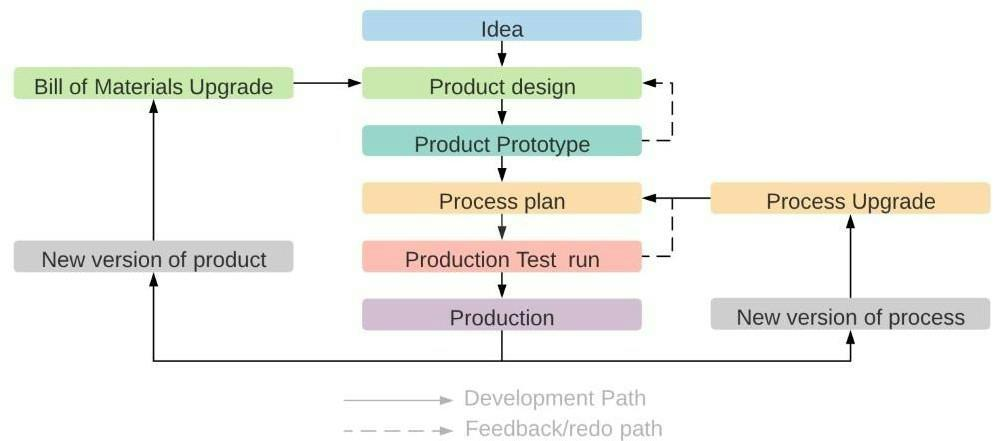
\includegraphics[width=434.28pt,height=191.8pt]{latexImage_b9c30a707b0e1320aa86adefb66c8f49.png}}
\end{picture}
\newpage
\begin{tikzpicture}[overlay]\path(0pt,0pt);\end{tikzpicture}
\begin{picture}(-5,0)(2.5,0)
\put(500.26,-727.616){\fontsize{12}{1}\usefont{T1}{ptm}{m}{n}\selectfont\color{color_29791}18}
\put(511.78,-727.616){\fontsize{12}{1}\usefont{T1}{ptm}{m}{n}\selectfont\color{color_29791} }
\put(63.024,-726.896){\fontsize{9.96}{1}\usefont{T1}{ptm}{m}{n}\selectfont\color{color_29791} }
\put(151.1,-366.64){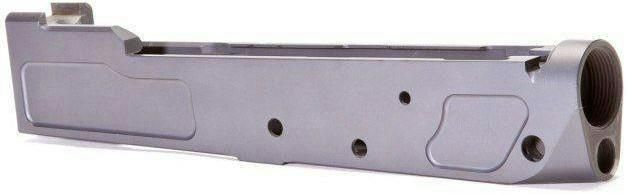
\includegraphics[width=289.1pt,height=88.743pt]{latexImage_9defbe0347eaef39f1e971809dcfed39.png}}
\put(426.31,-217.06){\fontsize{9.96}{1}\usefont{T1}{ptm}{m}{n}\selectfont\color{color_29791} }
\put(156.02,-243.85){\fontsize{12}{1}\usefont{T1}{ptm}{b}{n}\selectfont\color{color_29791}圖}
\put(168.02,-243.85){\fontsize{12}{1}\usefont{T1}{ptm}{b}{n}\selectfont\color{color_29791}10}
\put(180.05,-243.85){\fontsize{12}{1}\usefont{T1}{ptm}{b}{n}\selectfont\color{color_29791} }
\put(183.17,-243.85){\fontsize{12}{1}\usefont{T1}{ptm}{b}{n}\selectfont\color{color_29791}衝壓}
\put(207.17,-243.85){\fontsize{12}{1}\usefont{T1}{ptm}{b}{n}\selectfont\color{color_29791}AK74}
\put(237.17,-243.85){\fontsize{12}{1}\usefont{T1}{ptm}{b}{n}\selectfont\color{color_29791}式步槍機匣示例}
\put(321.19,-243.85){\fontsize{12}{1}\usefont{T1}{ptm}{b}{n}\selectfont\color{color_29791}(}
\put(333.07,-243.85){\fontsize{12}{1}\usefont{T1}{ptm}{b}{n}\selectfont\color{color_29791}B}
\put(340.99,-243.85){\fontsize{12}{1}\usefont{T1}{ptm}{b}{n}\selectfont\color{color_29791}r}
\put(346.15,-243.85){\fontsize{12}{1}\usefont{T1}{ptm}{b}{n}\selectfont\color{color_29791}o}
\put(352.03,-243.85){\fontsize{12}{1}\usefont{T1}{ptm}{b}{n}\selectfont\color{color_29791}w}
\put(360.55,-243.85){\fontsize{12}{1}\usefont{T1}{ptm}{b}{n}\selectfont\color{color_29791}n}
\put(367.15,-243.85){\fontsize{12}{1}\usefont{T1}{ptm}{b}{n}\selectfont\color{color_29791}n}
\put(373.75,-243.85){\fontsize{12}{1}\usefont{T1}{ptm}{b}{n}\selectfont\color{color_29791}e}
\put(378.91,-243.85){\fontsize{12}{1}\usefont{T1}{ptm}{b}{n}\selectfont\color{color_29791}l}
\put(382.15,-243.85){\fontsize{12}{1}\usefont{T1}{ptm}{b}{n}\selectfont\color{color_29791}l}
\put(385.39,-243.85){\fontsize{12}{1}\usefont{T1}{ptm}{b}{n}\selectfont\color{color_29791}s}
\put(389.95,-243.85){\fontsize{12}{1}\usefont{T1}{ptm}{b}{n}\selectfont\color{color_29791}.c}
\put(398.11,-243.85){\fontsize{12}{1}\usefont{T1}{ptm}{b}{n}\selectfont\color{color_29791}o}
\put(403.99,-243.85){\fontsize{12}{1}\usefont{T1}{ptm}{b}{n}\selectfont\color{color_29791}m}
\put(413.95,-243.85){\fontsize{12}{1}\usefont{T1}{ptm}{b}{n}\selectfont\color{color_29791})}
\put(425.83,-243.85){\fontsize{12}{1}\usefont{T1}{ptm}{b}{n}\selectfont\color{color_29791} }
\put(63.024,-271.09){\fontsize{9.96}{1}\usefont{T1}{ptm}{b}{n}\selectfont\color{color_29791} }
\put(63.024,-389.29){\fontsize{12}{1}\usefont{T1}{ptm}{b}{n}\selectfont\color{color_29791} }
\put(156.74,-410.07){\fontsize{12}{1}\usefont{T1}{ptm}{b}{n}\selectfont\color{color_29791}圖}
\put(168.74,-410.07){\fontsize{12}{1}\usefont{T1}{ptm}{b}{n}\selectfont\color{color_29791}11}
\put(180.77,-410.07){\fontsize{12}{1}\usefont{T1}{ptm}{b}{n}\selectfont\color{color_29791} }
\put(183.89,-410.07){\fontsize{12}{1}\usefont{T1}{ptm}{b}{n}\selectfont\color{color_29791}銑削}
\put(207.89,-410.07){\fontsize{12}{1}\usefont{T1}{ptm}{b}{n}\selectfont\color{color_29791}AK74}
\put(237.89,-410.07){\fontsize{12}{1}\usefont{T1}{ptm}{b}{n}\selectfont\color{color_29791}型步槍機匣示例}
\put(321.91,-410.07){\fontsize{12}{1}\usefont{T1}{ptm}{b}{n}\selectfont\color{color_29791}(}
\put(333.79,-410.07){\fontsize{12}{1}\usefont{T1}{ptm}{b}{n}\selectfont\color{color_29791}s}
\put(338.35,-410.07){\fontsize{12}{1}\usefont{T1}{ptm}{b}{n}\selectfont\color{color_29791}h}
\put(344.95,-410.07){\fontsize{12}{1}\usefont{T1}{ptm}{b}{n}\selectfont\color{color_29791}a}
\put(350.83,-410.07){\fontsize{12}{1}\usefont{T1}{ptm}{b}{n}\selectfont\color{color_29791}r}
\put(355.99,-410.07){\fontsize{12}{1}\usefont{T1}{ptm}{b}{n}\selectfont\color{color_29791}p}
\put(362.59,-410.07){\fontsize{12}{1}\usefont{T1}{ptm}{b}{n}\selectfont\color{color_29791}s}
\put(367.15,-410.07){\fontsize{12}{1}\usefont{T1}{ptm}{b}{n}\selectfont\color{color_29791}b}
\put(373.75,-410.07){\fontsize{12}{1}\usefont{T1}{ptm}{b}{n}\selectfont\color{color_29791}r}
\put(378.91,-410.07){\fontsize{12}{1}\usefont{T1}{ptm}{b}{n}\selectfont\color{color_29791}o}
\put(384.79,-410.07){\fontsize{12}{1}\usefont{T1}{ptm}{b}{n}\selectfont\color{color_29791}s}
\put(389.35,-410.07){\fontsize{12}{1}\usefont{T1}{ptm}{b}{n}\selectfont\color{color_29791}.c}
\put(397.51,-410.07){\fontsize{12}{1}\usefont{T1}{ptm}{b}{n}\selectfont\color{color_29791}o}
\put(403.39,-410.07){\fontsize{12}{1}\usefont{T1}{ptm}{b}{n}\selectfont\color{color_29791}m}
\put(413.35,-410.07){\fontsize{12}{1}\usefont{T1}{ptm}{b}{n}\selectfont\color{color_29791})}
\put(425.23,-410.07){\fontsize{12}{1}\usefont{T1}{ptm}{b}{n}\selectfont\color{color_29791} }
\put(82.944,-442.71){\fontsize{12}{1}\usefont{T1}{ptm}{m}{n}\selectfont\color{color_29791}就這家虛構的公司而言,已經確定,體現}
\put(298.97,-442.71){\fontsize{12}{1}\usefont{T1}{ptm}{m}{n}\selectfont\color{color_29791} }
\put(456.46,-442.71){\fontsize{12}{1}\usefont{T1}{ptm}{m}{n}\selectfont\color{color_29791}P}
\put(463.18,-442.71){\fontsize{12}{1}\usefont{T1}{ptm}{m}{n}\selectfont\color{color_29791}L}
\put(470.14,-442.71){\fontsize{12}{1}\usefont{T1}{ptm}{m}{n}\selectfont\color{color_29791}M}
\put(480.7,-442.71){\fontsize{12}{1}\usefont{T1}{ptm}{m}{n}\selectfont\color{color_29791}+}
\put(487.3,-442.71){\fontsize{12}{1}\usefont{T1}{ptm}{m}{n}\selectfont\color{color_29791}M}
\put(497.86,-442.71){\fontsize{12}{1}\usefont{T1}{ptm}{m}{n}\selectfont\color{color_29791}E}
\put(505.0601,-442.71){\fontsize{12}{1}\usefont{T1}{ptm}{m}{n}\selectfont\color{color_29791}S}
\put(69.384,-460.59){\fontsize{12}{1}\usefont{T1}{ptm}{m}{n}\selectfont\color{color_29791}效應的最佳方式是圍繞塑膠注射成型設計產品。乍一看,考慮這種製造程式似乎不}
\put(69.384,-478.59){\fontsize{12}{1}\usefont{T1}{ptm}{m}{n}\selectfont\color{color_29791}直}
\put(81.384,-478.59){\fontsize{12}{1}\usefont{T1}{ptm}{m}{n}\selectfont\color{color_29791}觀}
\put(93.38,-478.59){\fontsize{12}{1}\usefont{T1}{ptm}{m}{n}\selectfont\color{color_29791},就像前面描述的衝壓程式一樣,因為它在生產過程中也依賴於高精度模}
\put(477.46,-478.59){\fontsize{12}{1}\usefont{T1}{ptm}{m}{n}\selectfont\color{color_29791}具}
\put(489.46,-478.59){\fontsize{12}{1}\usefont{T1}{ptm}{m}{n}\selectfont\color{color_29791}。}
\put(69.384,-496.47){\fontsize{12}{1}\usefont{T1}{ptm}{m}{n}\selectfont\color{color_29791}然}
\put(81.384,-496.47){\fontsize{12}{1}\usefont{T1}{ptm}{m}{n}\selectfont\color{color_29791}而}
\put(93.38,-496.47){\fontsize{12}{1}\usefont{T1}{ptm}{m}{n}\selectfont\color{color_29791},兩者之間的主要區別在於原型製作的便利性和升級成}
\put(381.43,-496.47){\fontsize{12}{1}\usefont{T1}{ptm}{m}{n}\selectfont\color{color_29791}本}
\put(393.43,-496.47){\fontsize{12}{1}\usefont{T1}{ptm}{m}{n}\selectfont\color{color_29791}。}
\put(405.43,-496.47){\fontsize{12}{1}\usefont{T1}{ptm}{m}{n}\selectfont\color{color_29791} }
\put(63.024,-514.59){\fontsize{12}{1}\usefont{T1}{ptm}{m}{n}\selectfont\color{color_29791} }
\put(82.944,-530.19){\fontsize{12}{1}\usefont{T1}{ptm}{m}{n}\selectfont\color{color_29791}注塑成型是一個廣泛而複雜的工程領域,涉及種類繁多的材料和方法,其中很少}
\put(69.384,-548.07){\fontsize{12}{1}\usefont{T1}{ptm}{m}{n}\selectfont\color{color_29791}是這項}
\put(105.264,-548.07){\fontsize{12}{1}\usefont{T1}{ptm}{m}{n}\selectfont\color{color_29791}工作所}
\put(141.144,-548.07){\fontsize{12}{1}\usefont{T1}{ptm}{m}{n}\selectfont\color{color_29791}關注}
\put(165.024,-548.07){\fontsize{12}{1}\usefont{T1}{ptm}{m}{n}\selectfont\color{color_29791}的。}
\put(188.904,-548.07){\fontsize{12}{1}\usefont{T1}{ptm}{m}{n}\selectfont\color{color_29791}然而,}
\put(224.784,-548.07){\fontsize{12}{1}\usefont{T1}{ptm}{m}{n}\selectfont\color{color_29791}需要指}
\put(260.664,-548.07){\fontsize{12}{1}\usefont{T1}{ptm}{m}{n}\selectfont\color{color_29791}出的}
\put(284.544,-548.07){\fontsize{12}{1}\usefont{T1}{ptm}{m}{n}\selectfont\color{color_29791}是,}
\put(308.424,-548.07){\fontsize{12}{1}\usefont{T1}{ptm}{m}{n}\selectfont\color{color_29791}在大多}
\put(344.304,-548.07){\fontsize{12}{1}\usefont{T1}{ptm}{m}{n}\selectfont\color{color_29791}數情況}
\put(380.1841,-548.07){\fontsize{12}{1}\usefont{T1}{ptm}{m}{n}\selectfont\color{color_29791}下,}
\put(404.0641,-548.07){\fontsize{12}{1}\usefont{T1}{ptm}{m}{n}\selectfont\color{color_29791}注塑}
\put(427.9441,-548.07){\fontsize{12}{1}\usefont{T1}{ptm}{m}{n}\selectfont\color{color_29791}成型中}
\put(463.8241,-548.07){\fontsize{12}{1}\usefont{T1}{ptm}{m}{n}\selectfont\color{color_29791}涉及的}
\put(499.704,-548.07){\fontsize{12}{1}\usefont{T1}{ptm}{m}{n}\selectfont\color{color_29791}壓}
\put(69.384,-565.95){\fontsize{12}{1}\usefont{T1}{ptm}{m}{n}\selectfont\color{color_29791}力比我}
\put(105.264,-565.95){\fontsize{12}{1}\usefont{T1}{ptm}{m}{n}\selectfont\color{color_29791}們處理}
\put(141.144,-565.95){\fontsize{12}{1}\usefont{T1}{ptm}{m}{n}\selectfont\color{color_29791}鋼時}
\put(165.024,-565.95){\fontsize{12}{1}\usefont{T1}{ptm}{m}{n}\selectfont\color{color_29791}的壓}
\put(188.904,-565.95){\fontsize{12}{1}\usefont{T1}{ptm}{m}{n}\selectfont\color{color_29791}力低一}
\put(224.784,-565.95){\fontsize{12}{1}\usefont{T1}{ptm}{m}{n}\selectfont\color{color_29791}個數量}
\put(260.664,-565.95){\fontsize{12}{1}\usefont{T1}{ptm}{m}{n}\selectfont\color{color_29791}級}
\put(272.69,-565.95){\fontsize{12}{1}\usefont{T1}{ptm}{m}{n}\selectfont\color{color_29791};}
\put(276.05,-565.95){\fontsize{12}{1}\usefont{T1}{ptm}{m}{n}\selectfont\color{color_29791}較軟}
\put(299.93,-565.95){\fontsize{12}{1}\usefont{T1}{ptm}{m}{n}\selectfont\color{color_29791}的材料可用於他們的模具,例如}
\put(467.98,-565.95){\fontsize{12}{1}\usefont{T1}{ptm}{m}{n}\selectfont\color{color_29791} }
\put(473.98,-565.95){\fontsize{12}{1}\usefont{T1}{ptm}{m}{n}\selectfont\color{color_29791}C}
\put(481.78,-565.95){\fontsize{12}{1}\usefont{T1}{ptm}{m}{n}\selectfont\color{color_29791}N}
\put(490.18,-565.95){\fontsize{12}{1}\usefont{T1}{ptm}{m}{n}\selectfont\color{color_29791}C}
\put(497.98,-565.95){\fontsize{12}{1}\usefont{T1}{ptm}{m}{n}\selectfont\color{color_29791}銑}
\put(69.384,-583.86){\fontsize{12}{1}\usefont{T1}{ptm}{m}{n}\selectfont\color{color_29791}削鋁。}
\put(105.264,-583.86){\fontsize{12}{1}\usefont{T1}{ptm}{m}{n}\selectfont\color{color_29791}同時,}
\put(141.144,-583.86){\fontsize{12}{1}\usefont{T1}{ptm}{m}{n}\selectfont\color{color_29791}增材}
\put(165.024,-583.86){\fontsize{12}{1}\usefont{T1}{ptm}{m}{n}\selectfont\color{color_29791}製造}
\put(188.904,-583.86){\fontsize{12}{1}\usefont{T1}{ptm}{m}{n}\selectfont\color{color_29791}領域的}
\put(224.784,-583.86){\fontsize{12}{1}\usefont{T1}{ptm}{m}{n}\selectfont\color{color_29791}新進展}
\put(260.664,-583.86){\fontsize{12}{1}\usefont{T1}{ptm}{m}{n}\selectfont\color{color_29791}使得}
\put(284.544,-583.86){\fontsize{12}{1}\usefont{T1}{ptm}{m}{n}\selectfont\color{color_29791}塑膠}
\put(308.424,-583.86){\fontsize{12}{1}\usefont{T1}{ptm}{m}{n}\selectfont\color{color_29791}部件的}
\put(344.304,-583.86){\fontsize{12}{1}\usefont{T1}{ptm}{m}{n}\selectfont\color{color_29791}原型設}
\put(380.1841,-583.86){\fontsize{12}{1}\usefont{T1}{ptm}{m}{n}\selectfont\color{color_29791}計成}
\put(404.0641,-583.86){\fontsize{12}{1}\usefont{T1}{ptm}{m}{n}\selectfont\color{color_29791}為可}
\put(427.9441,-583.86){\fontsize{12}{1}\usefont{T1}{ptm}{m}{n}\selectfont\color{color_29791}能,這}
\put(463.8241,-583.86){\fontsize{12}{1}\usefont{T1}{ptm}{m}{n}\selectfont\color{color_29791}些塑膠}
\put(499.704,-583.86){\fontsize{12}{1}\usefont{T1}{ptm}{m}{n}\selectfont\color{color_29791}部}
\put(69.384,-601.86){\fontsize{12}{1}\usefont{T1}{ptm}{m}{n}\selectfont\color{color_29791}件的物}
\put(105.264,-601.86){\fontsize{12}{1}\usefont{T1}{ptm}{m}{n}\selectfont\color{color_29791}理特性}
\put(141.144,-601.86){\fontsize{12}{1}\usefont{T1}{ptm}{m}{n}\selectfont\color{color_29791}更接}
\put(165.024,-601.86){\fontsize{12}{1}\usefont{T1}{ptm}{m}{n}\selectfont\color{color_29791}近注}
\put(188.904,-601.86){\fontsize{12}{1}\usefont{T1}{ptm}{m}{n}\selectfont\color{color_29791}塑件的}
\put(224.784,-601.86){\fontsize{12}{1}\usefont{T1}{ptm}{m}{n}\selectfont\color{color_29791}最終結}
\put(260.664,-601.86){\fontsize{12}{1}\usefont{T1}{ptm}{m}{n}\selectfont\color{color_29791}果。}
\put(284.544,-601.86){\fontsize{12}{1}\usefont{T1}{ptm}{m}{n}\selectfont\color{color_29791}有時}
\put(308.424,-601.86){\fontsize{12}{1}\usefont{T1}{ptm}{m}{n}\selectfont\color{color_29791},在工}
\put(344.304,-601.86){\fontsize{12}{1}\usefont{T1}{ptm}{m}{n}\selectfont\color{color_29791}藝升級}
\put(380.1841,-601.86){\fontsize{12}{1}\usefont{T1}{ptm}{m}{n}\selectfont\color{color_29791}期間}
\put(404.0641,-601.86){\fontsize{12}{1}\usefont{T1}{ptm}{m}{n}\selectfont\color{color_29791},甚}
\put(427.9441,-601.86){\fontsize{12}{1}\usefont{T1}{ptm}{m}{n}\selectfont\color{color_29791}至可以}
\put(463.8241,-601.86){\fontsize{12}{1}\usefont{T1}{ptm}{m}{n}\selectfont\color{color_29791}使用原}
\put(499.704,-601.86){\fontsize{12}{1}\usefont{T1}{ptm}{m}{n}\selectfont\color{color_29791}型}
\put(69.384,-619.74){\fontsize{12}{1}\usefont{T1}{ptm}{m}{n}\selectfont\color{color_29791}模具}
\put(93.38,-619.74){\fontsize{12}{1}\usefont{T1}{ptm}{m}{n}\selectfont\color{color_29791}(}
\put(105.38,-619.74){\fontsize{12}{1}\usefont{T1}{ptm}{m}{n}\selectfont\color{color_29791}圖}
\put(115.82,-619.74){\fontsize{12}{1}\usefont{T1}{ptm}{m}{n}\selectfont\color{color_29791} }
\put(120.26,-619.74){\fontsize{12}{1}\usefont{T1}{ptm}{m}{n}\selectfont\color{color_29791}12}
\put(132.26,-619.74){\fontsize{12}{1}\usefont{T1}{ptm}{m}{n}\selectfont\color{color_29791})進行小批量測試。}
\put(240.29,-619.74){\fontsize{12}{1}\usefont{T1}{ptm}{m}{n}\selectfont\color{color_29791} }
\put(162.1,-216.98){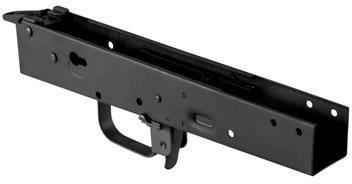
\includegraphics[width=264.15pt,height=137.98pt]{latexImage_b4cdf611b8c9603f9dc75a31af0f2a23.png}}
\end{picture}
\newpage
\begin{tikzpicture}[overlay]\path(0pt,0pt);\end{tikzpicture}
\begin{picture}(-5,0)(2.5,0)
\put(500.26,-727.616){\fontsize{12}{1}\usefont{T1}{ptm}{m}{n}\selectfont\color{color_29791}19}
\put(511.78,-727.616){\fontsize{12}{1}\usefont{T1}{ptm}{m}{n}\selectfont\color{color_29791} }
\put(63.024,-726.896){\fontsize{9.96}{1}\usefont{T1}{ptm}{m}{n}\selectfont\color{color_29791} }
\put(512.74,-352.81){\fontsize{9.96}{1}\usefont{T1}{ptm}{m}{n}\selectfont\color{color_29791} }
\put(129.02,-368.17){\fontsize{12}{1}\usefont{T1}{ptm}{b}{n}\selectfont\color{color_29791}圖}
\put(141.02,-368.17){\fontsize{12}{1}\usefont{T1}{ptm}{b}{n}\selectfont\color{color_29791}12 }
\put(156.02,-368.17){\fontsize{12}{1}\usefont{T1}{ptm}{b}{n}\selectfont\color{color_29791}使用}
\put(180.05,-368.17){\fontsize{12}{1}\usefont{T1}{ptm}{b}{n}\selectfont\color{color_29791}3D}
\put(194.69,-368.17){\fontsize{12}{1}\usefont{T1}{ptm}{b}{n}\selectfont\color{color_29791}列印機制作的注塑模具示例}
\put(338.71,-368.17){\fontsize{12}{1}\usefont{T1}{ptm}{b}{n}\selectfont\color{color_29791}(}
\put(350.59,-368.17){\fontsize{12}{1}\usefont{T1}{ptm}{b}{n}\selectfont\color{color_29791}t}
\put(354.43,-368.17){\fontsize{12}{1}\usefont{T1}{ptm}{b}{n}\selectfont\color{color_29791}h}
\put(361.03,-368.17){\fontsize{12}{1}\usefont{T1}{ptm}{b}{n}\selectfont\color{color_29791}e}
\put(366.19,-368.17){\fontsize{12}{1}\usefont{T1}{ptm}{b}{n}\selectfont\color{color_29791}f}
\put(370.03,-368.17){\fontsize{12}{1}\usefont{T1}{ptm}{b}{n}\selectfont\color{color_29791}a}
\put(375.91,-368.17){\fontsize{12}{1}\usefont{T1}{ptm}{b}{n}\selectfont\color{color_29791}b}
\put(382.618,-368.17){\fontsize{12}{1}\usefont{T1}{ptm}{b}{n}\selectfont\color{color_29791}r}
\put(387.778,-368.17){\fontsize{12}{1}\usefont{T1}{ptm}{b}{n}\selectfont\color{color_29791}i}
\put(391.018,-368.17){\fontsize{12}{1}\usefont{T1}{ptm}{b}{n}\selectfont\color{color_29791}c}
\put(396.178,-368.17){\fontsize{12}{1}\usefont{T1}{ptm}{b}{n}\selectfont\color{color_29791}at}
\put(406.018,-368.17){\fontsize{12}{1}\usefont{T1}{ptm}{b}{n}\selectfont\color{color_29791}o}
\put(411.898,-368.17){\fontsize{12}{1}\usefont{T1}{ptm}{b}{n}\selectfont\color{color_29791}r}
\put(417.178,-368.17){\fontsize{12}{1}\usefont{T1}{ptm}{b}{n}\selectfont\color{color_29791}.}
\put(420.058,-368.17){\fontsize{12}{1}\usefont{T1}{ptm}{b}{n}\selectfont\color{color_29791}c}
\put(425.218,-368.17){\fontsize{12}{1}\usefont{T1}{ptm}{b}{n}\selectfont\color{color_29791}o}
\put(431.098,-368.17){\fontsize{12}{1}\usefont{T1}{ptm}{b}{n}\selectfont\color{color_29791}m}
\put(441.1,-368.17){\fontsize{12}{1}\usefont{T1}{ptm}{b}{n}\selectfont\color{color_29791})}
\put(453.1,-368.17){\fontsize{12}{1}\usefont{T1}{ptm}{b}{n}\selectfont\color{color_29791} }
\put(82.944,-399.25){\fontsize{12}{1}\usefont{T1}{ptm}{m}{n}\selectfont\color{color_29791}增材製造已成為超}
\put(178.092,-399.25){\fontsize{12}{1}\usefont{T1}{ptm}{m}{n}\selectfont\color{color_29791}柔性}
\put(201.96,-399.25){\fontsize{12}{1}\usefont{T1}{ptm}{m}{n}\selectfont\color{color_29791}生產的絕佳工具。}
\put(297.108,-399.25){\fontsize{12}{1}\usefont{T1}{ptm}{m}{n}\selectfont\color{color_29791}這種}
\put(320.976,-399.25){\fontsize{12}{1}\usefont{T1}{ptm}{m}{n}\selectfont\color{color_29791}持續改進的心態,}
\put(416.124,-399.25){\fontsize{12}{1}\usefont{T1}{ptm}{m}{n}\selectfont\color{color_29791}尤其}
\put(439.992,-399.25){\fontsize{12}{1}\usefont{T1}{ptm}{m}{n}\selectfont\color{color_29791}是在原型設}
\put(69.384,-417.27){\fontsize{12}{1}\usefont{T1}{ptm}{m}{n}\selectfont\color{color_29791}計和反}
\put(105.264,-417.27){\fontsize{12}{1}\usefont{T1}{ptm}{m}{n}\selectfont\color{color_29791}覆運算}
\put(141.144,-417.27){\fontsize{12}{1}\usefont{T1}{ptm}{m}{n}\selectfont\color{color_29791}設計}
\put(165.024,-417.27){\fontsize{12}{1}\usefont{T1}{ptm}{m}{n}\selectfont\color{color_29791}方面}
\put(188.904,-417.27){\fontsize{12}{1}\usefont{T1}{ptm}{m}{n}\selectfont\color{color_29791},是精}
\put(224.784,-417.27){\fontsize{12}{1}\usefont{T1}{ptm}{m}{n}\selectfont\color{color_29791}益心態}
\put(260.664,-417.27){\fontsize{12}{1}\usefont{T1}{ptm}{m}{n}\selectfont\color{color_29791}的標}
\put(284.544,-417.27){\fontsize{12}{1}\usefont{T1}{ptm}{m}{n}\selectfont\color{color_29791}誌,}
\put(308.424,-417.27){\fontsize{12}{1}\usefont{T1}{ptm}{m}{n}\selectfont\color{color_29791}這種心}
\put(344.304,-417.27){\fontsize{12}{1}\usefont{T1}{ptm}{m}{n}\selectfont\color{color_29791}態在現}
\put(380.1841,-417.27){\fontsize{12}{1}\usefont{T1}{ptm}{m}{n}\selectfont\color{color_29791}代工}
\put(404.0641,-417.27){\fontsize{12}{1}\usefont{T1}{ptm}{m}{n}\selectfont\color{color_29791}業中}
\put(427.9441,-417.27){\fontsize{12}{1}\usefont{T1}{ptm}{m}{n}\selectfont\color{color_29791}是如此}
\put(463.8241,-417.27){\fontsize{12}{1}\usefont{T1}{ptm}{m}{n}\selectfont\color{color_29791}重要。}
\put(499.78,-417.27){\fontsize{12}{1}\usefont{T1}{ptm}{m}{n}\selectfont\color{color_29791} }
\put(63.024,-435.39){\fontsize{12}{1}\usefont{T1}{ptm}{m}{n}\selectfont\color{color_29791} }
\put(85.46,-450.87){\fontsize{12}{1}\usefont{T1}{ptm}{m}{n}\selectfont\color{color_29791}如}
\put(97.34,-450.87){\fontsize{12}{1}\usefont{T1}{ptm}{m}{n}\selectfont\color{color_29791}上}
\put(109.22,-450.87){\fontsize{12}{1}\usefont{T1}{ptm}{m}{n}\selectfont\color{color_29791}一}
\put(121.1,-450.87){\fontsize{12}{1}\usefont{T1}{ptm}{m}{n}\selectfont\color{color_29791}節}
\put(132.98,-450.87){\fontsize{12}{1}\usefont{T1}{ptm}{m}{n}\selectfont\color{color_29791}所}
\put(144.86,-450.87){\fontsize{12}{1}\usefont{T1}{ptm}{m}{n}\selectfont\color{color_29791}述}
\put(156.62,-450.87){\fontsize{12}{1}\usefont{T1}{ptm}{m}{n}\selectfont\color{color_29791},}
\put(168.5,-450.87){\fontsize{12}{1}\usefont{T1}{ptm}{m}{n}\selectfont\color{color_29791}在}
\put(180.38,-450.87){\fontsize{12}{1}\usefont{T1}{ptm}{m}{n}\selectfont\color{color_29791}本}
\put(192.26,-450.87){\fontsize{12}{1}\usefont{T1}{ptm}{m}{n}\selectfont\color{color_29791}案}
\put(204.02,-450.87){\fontsize{12}{1}\usefont{T1}{ptm}{m}{n}\selectfont\color{color_29791}例}
\put(215.9,-450.87){\fontsize{12}{1}\usefont{T1}{ptm}{m}{n}\selectfont\color{color_29791}研}
\put(227.78,-450.87){\fontsize{12}{1}\usefont{T1}{ptm}{m}{n}\selectfont\color{color_29791}究}
\put(239.66,-450.87){\fontsize{12}{1}\usefont{T1}{ptm}{m}{n}\selectfont\color{color_29791}中}
\put(251.54,-450.87){\fontsize{12}{1}\usefont{T1}{ptm}{m}{n}\selectfont\color{color_29791},}
\put(263.42,-450.87){\fontsize{12}{1}\usefont{T1}{ptm}{m}{n}\selectfont\color{color_29791}它}
\put(275.18,-450.87){\fontsize{12}{1}\usefont{T1}{ptm}{m}{n}\selectfont\color{color_29791}被}
\put(287.06,-450.87){\fontsize{12}{1}\usefont{T1}{ptm}{m}{n}\selectfont\color{color_29791}認}
\put(298.94,-450.87){\fontsize{12}{1}\usefont{T1}{ptm}{m}{n}\selectfont\color{color_29791}為}
\put(310.82,-450.87){\fontsize{12}{1}\usefont{T1}{ptm}{m}{n}\selectfont\color{color_29791}是}
\put(322.58,-450.87){\fontsize{12}{1}\usefont{T1}{ptm}{m}{n}\selectfont\color{color_29791}虛}
\put(334.4601,-450.87){\fontsize{12}{1}\usefont{T1}{ptm}{m}{n}\selectfont\color{color_29791}構}
\put(346.3401,-450.87){\fontsize{12}{1}\usefont{T1}{ptm}{m}{n}\selectfont\color{color_29791}公}
\put(358.2201,-450.87){\fontsize{12}{1}\usefont{T1}{ptm}{m}{n}\selectfont\color{color_29791}司}
\put(370.1001,-450.87){\fontsize{12}{1}\usefont{T1}{ptm}{m}{n}\selectfont\color{color_29791}創}
\put(381.9801,-450.87){\fontsize{12}{1}\usefont{T1}{ptm}{m}{n}\selectfont\color{color_29791}造}
\put(393.7401,-450.87){\fontsize{12}{1}\usefont{T1}{ptm}{m}{n}\selectfont\color{color_29791}新}
\put(405.6201,-450.87){\fontsize{12}{1}\usefont{T1}{ptm}{m}{n}\selectfont\color{color_29791}產}
\put(417.5001,-450.87){\fontsize{12}{1}\usefont{T1}{ptm}{m}{n}\selectfont\color{color_29791}品}
\put(429.3801,-450.87){\fontsize{12}{1}\usefont{T1}{ptm}{m}{n}\selectfont\color{color_29791}及}
\put(441.1401,-450.87){\fontsize{12}{1}\usefont{T1}{ptm}{m}{n}\selectfont\color{color_29791}其}
\put(453.0201,-450.87){\fontsize{12}{1}\usefont{T1}{ptm}{m}{n}\selectfont\color{color_29791}生}
\put(464.9001,-450.87){\fontsize{12}{1}\usefont{T1}{ptm}{m}{n}\selectfont\color{color_29791}產}
\put(476.7801,-450.87){\fontsize{12}{1}\usefont{T1}{ptm}{m}{n}\selectfont\color{color_29791}過}
\put(488.6601,-450.87){\fontsize{12}{1}\usefont{T1}{ptm}{m}{n}\selectfont\color{color_29791}程}
\put(500.5,-450.87){\fontsize{12}{1}\usefont{T1}{ptm}{m}{n}\selectfont\color{color_29791} }
\put(69.384,-468.75){\fontsize{12}{1}\usefont{T1}{ptm}{m}{n}\selectfont\color{color_29791}。該產品由一個塑膠小型計算機機箱組成,由}
\put(309.43,-468.75){\fontsize{15}{1}\usefont{T1}{ptm}{m}{n}\selectfont\color{color_29791}  }
\put(335.35,-468.75){\fontsize{12}{1}\usefont{T1}{ptm}{m}{n}\selectfont\color{color_29791}3}
\put(341.47,-468.75){\fontsize{12}{1}\usefont{T1}{ptm}{m}{n}\selectfont\color{color_29791} }
\put(392.47,-468.75){\fontsize{12}{1}\usefont{T1}{ptm}{m}{n}\selectfont\color{color_29791}個不同}
\put(428.578,-468.75){\fontsize{12}{1}\usefont{T1}{ptm}{m}{n}\selectfont\color{color_29791}的部件}
\put(464.686,-468.75){\fontsize{12}{1}\usefont{T1}{ptm}{m}{n}\selectfont\color{color_29791}組成(}
\put(500.794,-468.75){\fontsize{12}{1}\usefont{T1}{ptm}{m}{n}\selectfont\color{color_29791}圖}
\put(512.86,-468.75){\fontsize{12}{1}\usefont{T1}{ptm}{m}{n}\selectfont\color{color_29791} }
\put(69.384,-486.75){\fontsize{12}{1}\usefont{T1}{ptm}{m}{n}\selectfont\color{color_29791}13}
\put(81.144,-486.75){\fontsize{12}{1}\usefont{T1}{ptm}{m}{n}\selectfont\color{color_29791})}
\put(93.02399,-486.75){\fontsize{12}{1}\usefont{T1}{ptm}{m}{n}\selectfont\color{color_29791},}
\put(104.904,-486.75){\fontsize{12}{1}\usefont{T1}{ptm}{m}{n}\selectfont\color{color_29791}預}
\put(116.784,-486.75){\fontsize{12}{1}\usefont{T1}{ptm}{m}{n}\selectfont\color{color_29791}計}
\put(128.664,-486.75){\fontsize{12}{1}\usefont{T1}{ptm}{m}{n}\selectfont\color{color_29791}這}
\put(140.544,-486.75){\fontsize{12}{1}\usefont{T1}{ptm}{m}{n}\selectfont\color{color_29791}些部}
\put(164.424,-486.75){\fontsize{12}{1}\usefont{T1}{ptm}{m}{n}\selectfont\color{color_29791}件}
\put(176.304,-486.75){\fontsize{12}{1}\usefont{T1}{ptm}{m}{n}\selectfont\color{color_29791}的設}
\put(200.184,-486.75){\fontsize{12}{1}\usefont{T1}{ptm}{m}{n}\selectfont\color{color_29791}計}
\put(212.064,-486.75){\fontsize{12}{1}\usefont{T1}{ptm}{m}{n}\selectfont\color{color_29791}和}
\put(223.944,-486.75){\fontsize{12}{1}\usefont{T1}{ptm}{m}{n}\selectfont\color{color_29791}原}
\put(235.824,-486.75){\fontsize{12}{1}\usefont{T1}{ptm}{m}{n}\selectfont\color{color_29791}型}
\put(247.704,-486.75){\fontsize{12}{1}\usefont{T1}{ptm}{m}{n}\selectfont\color{color_29791}設}
\put(259.584,-486.75){\fontsize{12}{1}\usefont{T1}{ptm}{m}{n}\selectfont\color{color_29791}計}
\put(271.4641,-486.75){\fontsize{12}{1}\usefont{T1}{ptm}{m}{n}\selectfont\color{color_29791}將結}
\put(295.3441,-486.75){\fontsize{12}{1}\usefont{T1}{ptm}{m}{n}\selectfont\color{color_29791}合增}
\put(319.2241,-486.75){\fontsize{12}{1}\usefont{T1}{ptm}{m}{n}\selectfont\color{color_29791}材}
\put(331.1041,-486.75){\fontsize{12}{1}\usefont{T1}{ptm}{m}{n}\selectfont\color{color_29791}製}
\put(342.9841,-486.75){\fontsize{12}{1}\usefont{T1}{ptm}{m}{n}\selectfont\color{color_29791}造}
\put(354.8641,-486.75){\fontsize{12}{1}\usefont{T1}{ptm}{m}{n}\selectfont\color{color_29791}和}
\put(366.91,-486.75){\fontsize{12}{1}\usefont{T1}{ptm}{m}{n}\selectfont\color{color_29791} }
\put(392.47,-486.75){\fontsize{12}{1}\usefont{T1}{ptm}{m}{n}\selectfont\color{color_29791} }
\put(487.9,-486.75){\fontsize{12}{1}\usefont{T1}{ptm}{m}{n}\selectfont\color{color_29791}C}
\put(495.7,-486.75){\fontsize{12}{1}\usefont{T1}{ptm}{m}{n}\selectfont\color{color_29791}N}
\put(504.1,-486.75){\fontsize{12}{1}\usefont{T1}{ptm}{m}{n}\selectfont\color{color_29791}C}
\put(69.384,-504.63){\fontsize{12}{1}\usefont{T1}{ptm}{m}{n}\selectfont\color{color_29791}銑削以實現塑膠注}
\put(164.532,-504.63){\fontsize{12}{1}\usefont{T1}{ptm}{m}{n}\selectfont\color{color_29791}射成}
\put(188.4,-504.63){\fontsize{12}{1}\usefont{T1}{ptm}{m}{n}\selectfont\color{color_29791}型生產。}
\put(236.09,-504.63){\fontsize{12}{1}\usefont{T1}{ptm}{m}{n}\selectfont\color{color_29791} }
\put(73.75,-352.79){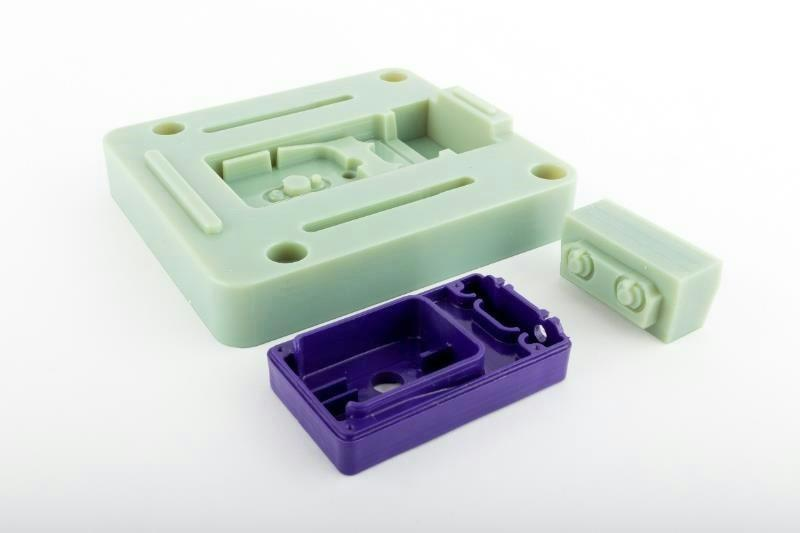
\includegraphics[width=438.95pt,height=291.79pt]{latexImage_6500d3903782332928e698fe9c4255e5.png}}
\end{picture}
\newpage
\begin{tikzpicture}[overlay]\path(0pt,0pt);\end{tikzpicture}
\begin{picture}(-5,0)(2.5,0)
\put(500.26,-727.616){\fontsize{12}{1}\usefont{T1}{ptm}{m}{n}\selectfont\color{color_29791}20}
\put(511.78,-727.616){\fontsize{12}{1}\usefont{T1}{ptm}{m}{n}\selectfont\color{color_29791} }
\put(63.024,-726.896){\fontsize{9.96}{1}\usefont{T1}{ptm}{m}{n}\selectfont\color{color_29791} }
\put(513.94,-385.33){\fontsize{9.96}{1}\usefont{T1}{ptm}{m}{n}\selectfont\color{color_29791} }
\put(222.41,-408.75){\fontsize{12}{1}\usefont{T1}{ptm}{b}{n}\selectfont\color{color_29791}圖}
\put(234.41,-408.75){\fontsize{12}{1}\usefont{T1}{ptm}{b}{n}\selectfont\color{color_29791}13 }
\put(249.41,-408.75){\fontsize{12}{1}\usefont{T1}{ptm}{b}{n}\selectfont\color{color_29791}理論乘積的}
\put(309.43,-408.75){\fontsize{12}{1}\usefont{T1}{ptm}{b}{n}\selectfont\color{color_29791}3D}
\put(324.07,-408.75){\fontsize{12}{1}\usefont{T1}{ptm}{b}{n}\selectfont\color{color_29791}分}
\put(335.95,-408.75){\fontsize{12}{1}\usefont{T1}{ptm}{b}{n}\selectfont\color{color_29791}解}
\put(347.71,-408.75){\fontsize{12}{1}\usefont{T1}{ptm}{b}{n}\selectfont\color{color_29791}圖}
\put(359.59,-408.75){\fontsize{12}{1}\usefont{T1}{ptm}{b}{n}\selectfont\color{color_29791} }
\put(63.024,-438.15){\fontsize{12.96}{1}\usefont{T1}{ptm}{b}{n}\selectfont\color{color_29791} }
\put(105.38,-460.71){\fontsize{12.81913}{1}\usefont{T1}{ptm}{b}{n}\selectfont\color{color_29791}4.}
\put(114.9648,-460.71){\fontsize{12.81913}{1}\usefont{T1}{ptm}{b}{n}\selectfont\color{color_29791}1}
\put(121.4307,-460.71){\fontsize{12.81913}{1}\usefont{T1}{ptm}{b}{n}\selectfont\color{color_29791}.}
\put(124.5495,-460.71){\fontsize{12.81913}{1}\usefont{T1}{ptm}{b}{n}\selectfont\color{color_29791}1}
\put(131.0154,-460.71){\fontsize{12.81913}{1}\usefont{T1}{ptm}{b}{n}\selectfont\color{color_29791}.}
\put(134.3,-460.71){\fontsize{12.83539}{1}\usefont{T1}{ptm}{b}{n}\selectfont\color{color_29791} }
\put(137.06,-460.71){\fontsize{12.96}{1}\usefont{T1}{ptm}{b}{n}\selectfont\color{color_29791}A}
\put(146.3,-460.71){\fontsize{12.96}{1}\usefont{T1}{ptm}{b}{n}\selectfont\color{color_29791}部分}
\put(171.74,-460.71){\fontsize{12.96}{1}\usefont{T1}{ptm}{b}{n}\selectfont\color{color_29791} }
\put(82.944,-488.55){\fontsize{12}{1}\usefont{T1}{ptm}{m}{n}\selectfont\color{color_29791}P}
\put(89.544,-488.55){\fontsize{12}{1}\usefont{T1}{ptm}{m}{n}\selectfont\color{color_29791}A}
\put(98.064,-488.55){\fontsize{12}{1}\usefont{T1}{ptm}{m}{n}\selectfont\color{color_29791}R}
\put(105.984,-488.55){\fontsize{12}{1}\usefont{T1}{ptm}{m}{n}\selectfont\color{color_29791}T}
\put(113.18,-488.55){\fontsize{12}{1}\usefont{T1}{ptm}{m}{n}\selectfont\color{color_29791}-}
\put(117.14,-488.55){\fontsize{12}{1}\usefont{T1}{ptm}{m}{n}\selectfont\color{color_29791} }
\put(69.384,-504.63){\fontsize{12}{1}\usefont{T1}{ptm}{m}{n}\selectfont\color{color_29791}A}
\put(78.024,-504.63){\fontsize{12}{1}\usefont{T1}{ptm}{m}{n}\selectfont\color{color_29791}(}
\put(90.02,-504.63){\fontsize{12}{1}\usefont{T1}{ptm}{m}{n}\selectfont\color{color_29791}圖}
\put(102.02,-504.63){\fontsize{12}{1}\usefont{T1}{ptm}{m}{n}\selectfont\color{color_29791}14}
\put(114.02,-504.63){\fontsize{12}{1}\usefont{T1}{ptm}{m}{n}\selectfont\color{color_29791})}
\put(126.02,-504.63){\fontsize{12}{1}\usefont{T1}{ptm}{m}{n}\selectfont\color{color_29791}是計}
\put(149.9,-504.63){\fontsize{12}{1}\usefont{T1}{ptm}{m}{n}\selectfont\color{color_29791}算機}
\put(173.78,-504.63){\fontsize{12}{1}\usefont{T1}{ptm}{m}{n}\selectfont\color{color_29791}機}
\put(185.66,-504.63){\fontsize{12}{1}\usefont{T1}{ptm}{m}{n}\selectfont\color{color_29791}箱的核}
\put(221.54,-504.63){\fontsize{12}{1}\usefont{T1}{ptm}{m}{n}\selectfont\color{color_29791}心結構}
\put(257.42,-504.63){\fontsize{12}{1}\usefont{T1}{ptm}{m}{n}\selectfont\color{color_29791}。預}
\put(281.3,-504.63){\fontsize{12}{1}\usefont{T1}{ptm}{m}{n}\selectfont\color{color_29791}計它}
\put(305.18,-504.63){\fontsize{12}{1}\usefont{T1}{ptm}{m}{n}\selectfont\color{color_29791}將包含}
\put(341.06,-504.63){\fontsize{12}{1}\usefont{T1}{ptm}{m}{n}\selectfont\color{color_29791}所討論}
\put(376.94,-504.63){\fontsize{12}{1}\usefont{T1}{ptm}{m}{n}\selectfont\color{color_29791}的小}
\put(400.82,-504.63){\fontsize{12}{1}\usefont{T1}{ptm}{m}{n}\selectfont\color{color_29791}型電}
\put(424.7,-504.63){\fontsize{12}{1}\usefont{T1}{ptm}{m}{n}\selectfont\color{color_29791}腦正常}
\put(460.58,-504.63){\fontsize{12}{1}\usefont{T1}{ptm}{m}{n}\selectfont\color{color_29791}運行所}
\put(496.4601,-504.63){\fontsize{12}{1}\usefont{T1}{ptm}{m}{n}\selectfont\color{color_29791}需}
\put(69.384,-522.51){\fontsize{12}{1}\usefont{T1}{ptm}{m}{n}\selectfont\color{color_29791}的所有}
\put(105.264,-522.51){\fontsize{12}{1}\usefont{T1}{ptm}{m}{n}\selectfont\color{color_29791}部件。}
\put(141.144,-522.51){\fontsize{12}{1}\usefont{T1}{ptm}{m}{n}\selectfont\color{color_29791}為此}
\put(165.024,-522.51){\fontsize{12}{1}\usefont{T1}{ptm}{m}{n}\selectfont\color{color_29791},選}
\put(188.904,-522.51){\fontsize{12}{1}\usefont{T1}{ptm}{m}{n}\selectfont\color{color_29791}擇了一}
\put(224.784,-522.51){\fontsize{12}{1}\usefont{T1}{ptm}{m}{n}\selectfont\color{color_29791}種原料}
\put(260.69,-522.51){\fontsize{12}{1}\usefont{T1}{ptm}{m}{n}\selectfont\color{color_29791}A}
\put(269.33,-522.51){\fontsize{12}{1}\usefont{T1}{ptm}{m}{n}\selectfont\color{color_29791},即丙}
\put(305.21,-522.51){\fontsize{12}{1}\usefont{T1}{ptm}{m}{n}\selectfont\color{color_29791}烯腈丁二烯苯乙烯(}
\put(413.23,-522.51){\fontsize{12}{1}\usefont{T1}{ptm}{m}{n}\selectfont\color{color_29791}A}
\put(421.87,-522.51){\fontsize{12}{1}\usefont{T1}{ptm}{m}{n}\selectfont\color{color_29791}B}
\put(429.79,-522.51){\fontsize{12}{1}\usefont{T1}{ptm}{m}{n}\selectfont\color{color_29791}S}
\put(436.51,-522.51){\fontsize{12}{1}\usefont{T1}{ptm}{m}{n}\selectfont\color{color_29791}),這是一種}
\put(69.384,-540.39){\fontsize{12}{1}\usefont{T1}{ptm}{m}{n}\selectfont\color{color_29791}不透明的熱塑性聚合物和工程級塑膠。它通常用於生產電子零件,如手機適配器、}
\put(69.384,-558.27){\fontsize{12}{1}\usefont{T1}{ptm}{m}{n}\selectfont\color{color_29791}鍵盤鍵和牆壁插座塑膠護罩。}
\put(225.41,-558.27){\fontsize{12}{1}\usefont{T1}{ptm}{m}{n}\selectfont\color{color_29791} }
\put(73.75,-385.29){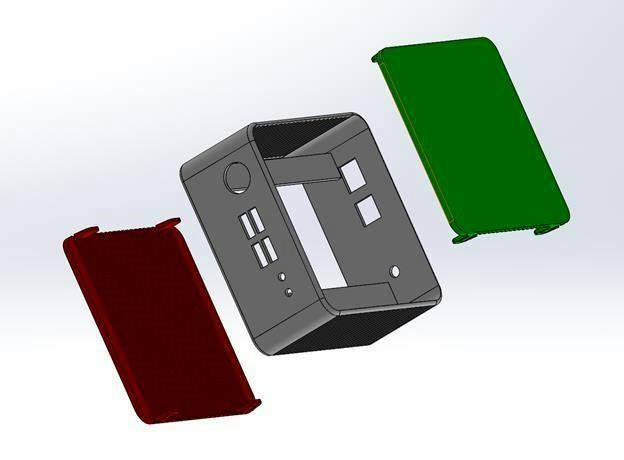
\includegraphics[width=440.05pt,height=324.29pt]{latexImage_ad633aedccef8b85100fc28bdf9d65c4.png}}
\end{picture}
\newpage
\begin{tikzpicture}[overlay]\path(0pt,0pt);\end{tikzpicture}
\begin{picture}(-5,0)(2.5,0)
\put(500.26,-727.616){\fontsize{12}{1}\usefont{T1}{ptm}{m}{n}\selectfont\color{color_29791}21}
\put(511.78,-727.616){\fontsize{12}{1}\usefont{T1}{ptm}{m}{n}\selectfont\color{color_29791} }
\put(63.024,-726.896){\fontsize{9.96}{1}\usefont{T1}{ptm}{m}{n}\selectfont\color{color_29791} }
\put(522.1,-263.41){\fontsize{9.96}{1}\usefont{T1}{ptm}{m}{n}\selectfont\color{color_29791} }
\put(221.45,-279.61){\fontsize{12}{1}\usefont{T1}{ptm}{b}{n}\selectfont\color{color_29791}圖}
\put(233.45,-279.61){\fontsize{12}{1}\usefont{T1}{ptm}{b}{n}\selectfont\color{color_29791} }
\put(236.45,-279.61){\fontsize{12}{1}\usefont{T1}{ptm}{b}{n}\selectfont\color{color_29791}14}
\put(248.45,-279.61){\fontsize{12}{1}\usefont{T1}{ptm}{b}{n}\selectfont\color{color_29791} }
\put(251.33,-279.61){\fontsize{12}{1}\usefont{T1}{ptm}{b}{n}\selectfont\color{color_29791}零件}
\put(275.33,-279.61){\fontsize{12}{1}\usefont{T1}{ptm}{b}{n}\selectfont\color{color_29791} }
\put(278.33,-279.61){\fontsize{12}{1}\usefont{T1}{ptm}{b}{n}\selectfont\color{color_29791}A}
\put(286.97,-279.61){\fontsize{12}{1}\usefont{T1}{ptm}{b}{n}\selectfont\color{color_29791} }
\put(289.25,-279.61){\fontsize{12}{1}\usefont{T1}{ptm}{b}{n}\selectfont\color{color_29791}的}
\put(301.13,-279.61){\fontsize{12}{1}\usefont{T1}{ptm}{b}{n}\selectfont\color{color_29791}等}
\put(313.01,-279.61){\fontsize{12}{1}\usefont{T1}{ptm}{b}{n}\selectfont\color{color_29791}軸}
\put(324.89,-279.61){\fontsize{12}{1}\usefont{T1}{ptm}{b}{n}\selectfont\color{color_29791}測檢}
\put(348.77,-279.61){\fontsize{12}{1}\usefont{T1}{ptm}{b}{n}\selectfont\color{color_29791}視}
\put(360.67,-279.61){\fontsize{12}{1}\usefont{T1}{ptm}{b}{n}\selectfont\color{color_29791} }
\put(82.944,-311.41){\fontsize{12}{1}\usefont{T1}{ptm}{m}{n}\selectfont\color{color_29791}特別選擇這種材料的主要原因是它的韌性、良好的尺寸穩定性(冷卻后不改變尺}
\put(69.384,-329.29){\fontsize{12}{1}\usefont{T1}{ptm}{m}{n}\selectfont\color{color_29791}寸)、高抗衝擊性和表}
\put(189.492,-329.29){\fontsize{12}{1}\usefont{T1}{ptm}{m}{n}\selectfont\color{color_29791}面硬度。最後,它通常}
\put(309.6,-329.29){\fontsize{12}{1}\usefont{T1}{ptm}{m}{n}\selectfont\color{color_29791}也以}
\put(333.67,-329.29){\fontsize{12}{1}\usefont{T1}{ptm}{m}{n}\selectfont\color{color_29791}3D}
\put(348.19,-329.29){\fontsize{12}{1}\usefont{T1}{ptm}{m}{n}\selectfont\color{color_29791}列印長絲的形}
\put(420.298,-329.29){\fontsize{12}{1}\usefont{T1}{ptm}{m}{n}\selectfont\color{color_29791}式}
\put(432.406,-329.29){\fontsize{12}{1}\usefont{T1}{ptm}{m}{n}\selectfont\color{color_29791}用於擠出}
\put(480.46,-329.29){\fontsize{12}{1}\usefont{T1}{ptm}{m}{n}\selectfont\color{color_29791}3D}
\put(494.98,-329.29){\fontsize{12}{1}\usefont{T1}{ptm}{m}{n}\selectfont\color{color_29791}印}
\put(69.384,-347.17){\fontsize{12}{1}\usefont{T1}{ptm}{m}{n}\selectfont\color{color_29791}表機,這應該在原}
\put(164.532,-347.17){\fontsize{12}{1}\usefont{T1}{ptm}{m}{n}\selectfont\color{color_29791}型製}
\put(188.4,-347.17){\fontsize{12}{1}\usefont{T1}{ptm}{m}{n}\selectfont\color{color_29791}作過程中被證明非}
\put(283.548,-347.17){\fontsize{12}{1}\usefont{T1}{ptm}{m}{n}\selectfont\color{color_29791}常有}
\put(307.416,-347.17){\fontsize{12}{1}\usefont{T1}{ptm}{m}{n}\selectfont\color{color_29791}用。}
\put(331.27,-347.17){\fontsize{12}{1}\usefont{T1}{ptm}{m}{n}\selectfont\color{color_29791} }
\put(63.024,-365.05){\fontsize{12}{1}\usefont{T1}{ptm}{m}{n}\selectfont\color{color_29791} }
\put(63.024,-383.89){\fontsize{12}{1}\usefont{T1}{ptm}{m}{n}\selectfont\color{color_29791} }
\put(105.38,-403.93){\fontsize{12.81913}{1}\usefont{T1}{ptm}{b}{n}\selectfont\color{color_29791}4.}
\put(114.9648,-403.93){\fontsize{12.81913}{1}\usefont{T1}{ptm}{b}{n}\selectfont\color{color_29791}1}
\put(121.4307,-403.93){\fontsize{12.81913}{1}\usefont{T1}{ptm}{b}{n}\selectfont\color{color_29791}.}
\put(124.5495,-403.93){\fontsize{12.81913}{1}\usefont{T1}{ptm}{b}{n}\selectfont\color{color_29791}2}
\put(131.0154,-403.93){\fontsize{12.81913}{1}\usefont{T1}{ptm}{b}{n}\selectfont\color{color_29791}.}
\put(134.3,-403.93){\fontsize{12.83539}{1}\usefont{T1}{ptm}{b}{n}\selectfont\color{color_29791} }
\put(137.66,-403.93){\fontsize{12.96}{1}\usefont{T1}{ptm}{b}{n}\selectfont\color{color_29791}B}
\put(146.3,-403.93){\fontsize{12.96}{1}\usefont{T1}{ptm}{b}{n}\selectfont\color{color_29791} }
\put(149.3,-403.93){\fontsize{12.96}{1}\usefont{T1}{ptm}{b}{n}\selectfont\color{color_29791}和}
\put(162.26,-403.93){\fontsize{12.96}{1}\usefont{T1}{ptm}{b}{n}\selectfont\color{color_29791} }
\put(165.5,-403.93){\fontsize{12.96}{1}\usefont{T1}{ptm}{b}{n}\selectfont\color{color_29791}C}
\put(174.86,-403.93){\fontsize{12.96}{1}\usefont{T1}{ptm}{b}{n}\selectfont\color{color_29791} }
\put(177.98,-403.93){\fontsize{12.96}{1}\usefont{T1}{ptm}{b}{n}\selectfont\color{color_29791}部分}
\put(203.69,-403.93){\fontsize{12.96}{1}\usefont{T1}{ptm}{b}{n}\selectfont\color{color_29791} }
\put(82.944,-432.51){\fontsize{12}{1}\usefont{T1}{ptm}{m}{n}\selectfont\color{color_29791}B}
\put(90.98,-432.51){\fontsize{12}{1}\usefont{T1}{ptm}{m}{n}\selectfont\color{color_29791} }
\put(291.77,-432.51){\fontsize{12}{1}\usefont{T1}{ptm}{m}{n}\selectfont\color{color_29791}和}
\put(303.77,-432.51){\fontsize{12}{1}\usefont{T1}{ptm}{m}{n}\selectfont\color{color_29791} }
\put(504.7,-432.51){\fontsize{12}{1}\usefont{T1}{ptm}{m}{n}\selectfont\color{color_29791}C}
\put(69.384,-450.15){\fontsize{12}{1}\usefont{T1}{ptm}{m}{n}\selectfont\color{color_29791}部分是蓋}
\put(117.38,-450.15){\fontsize{12}{1}\usefont{T1}{ptm}{m}{n}\selectfont\color{color_29791}子}
\put(129.38,-450.15){\fontsize{12}{1}\usefont{T1}{ptm}{m}{n}\selectfont\color{color_29791},應卡入到位,關閉系統。這些是非常簡單的部件,需要一定程度的彈}
\put(69.384,-467.91){\fontsize{12}{1}\usefont{T1}{ptm}{m}{n}\selectfont\color{color_29791}性}
\put(81.384,-467.91){\fontsize{12}{1}\usefont{T1}{ptm}{m}{n}\selectfont\color{color_29791},}
\put(93.38,-467.91){\fontsize{12}{1}\usefont{T1}{ptm}{m}{n}\selectfont\color{color_29791}因此它可以變形以確保無螺絲組裝。這兩個相同的部件將由熱塑性聚氨酯}
\put(477.46,-467.91){\fontsize{12}{1}\usefont{T1}{ptm}{m}{n}\selectfont\color{color_29791} }
\put(69.384,-485.79){\fontsize{12}{1}\usefont{T1}{ptm}{m}{n}\selectfont\color{color_29791}(}
\put(81.384,-485.79){\fontsize{12}{1}\usefont{T1}{ptm}{m}{n}\selectfont\color{color_29791}T}
\put(88.7,-485.79){\fontsize{12}{1}\usefont{T1}{ptm}{m}{n}\selectfont\color{color_29791}P}
\put(95.42,-485.79){\fontsize{12}{1}\usefont{T1}{ptm}{m}{n}\selectfont\color{color_29791}U}
\put(104.06,-485.79){\fontsize{12}{1}\usefont{T1}{ptm}{m}{n}\selectfont\color{color_29791})}
\put(115.94,-485.79){\fontsize{12}{1}\usefont{T1}{ptm}{m}{n}\selectfont\color{color_29791} }
\put(248.57,-485.79){\fontsize{12}{1}\usefont{T1}{ptm}{m}{n}\selectfont\color{color_29791}製成,}
\put(284.45,-485.79){\fontsize{12}{1}\usefont{T1}{ptm}{m}{n}\selectfont\color{color_29791}因為它}
\put(320.33,-485.79){\fontsize{12}{1}\usefont{T1}{ptm}{m}{n}\selectfont\color{color_29791}具有}
\put(344.21,-485.79){\fontsize{12}{1}\usefont{T1}{ptm}{m}{n}\selectfont\color{color_29791}彈性}
\put(368.09,-485.79){\fontsize{12}{1}\usefont{T1}{ptm}{m}{n}\selectfont\color{color_29791}和出色}
\put(403.97,-485.79){\fontsize{12}{1}\usefont{T1}{ptm}{m}{n}\selectfont\color{color_29791}的拉伸}
\put(439.85,-485.79){\fontsize{12}{1}\usefont{T1}{ptm}{m}{n}\selectfont\color{color_29791}和撕}
\put(463.73,-485.79){\fontsize{12}{1}\usefont{T1}{ptm}{m}{n}\selectfont\color{color_29791}裂強}
\put(487.61,-485.79){\fontsize{12}{1}\usefont{T1}{ptm}{m}{n}\selectfont\color{color_29791}度。}
\put(69.384,-503.67){\fontsize{12}{1}\usefont{T1}{ptm}{m}{n}\selectfont\color{color_29791}這種聚合物通常用於生產需要類似橡膠彈性的零件。熱塑性聚氨酯在高溫下表現良}
\put(69.384,-521.55){\fontsize{12}{1}\usefont{T1}{ptm}{m}{n}\selectfont\color{color_29791}好,常}
\put(105.264,-521.55){\fontsize{12}{1}\usefont{T1}{ptm}{m}{n}\selectfont\color{color_29791}用於電}
\put(141.144,-521.55){\fontsize{12}{1}\usefont{T1}{ptm}{m}{n}\selectfont\color{color_29791}動工}
\put(165.024,-521.55){\fontsize{12}{1}\usefont{T1}{ptm}{m}{n}\selectfont\color{color_29791}具、}
\put(188.904,-521.55){\fontsize{12}{1}\usefont{T1}{ptm}{m}{n}\selectfont\color{color_29791}電纜絕}
\put(224.784,-521.55){\fontsize{12}{1}\usefont{T1}{ptm}{m}{n}\selectfont\color{color_29791}緣層和}
\put(260.664,-521.55){\fontsize{12}{1}\usefont{T1}{ptm}{m}{n}\selectfont\color{color_29791}體育}
\put(284.544,-521.55){\fontsize{12}{1}\usefont{T1}{ptm}{m}{n}\selectfont\color{color_29791}用品}
\put(308.424,-521.55){\fontsize{12}{1}\usefont{T1}{ptm}{m}{n}\selectfont\color{color_29791}。最後}
\put(344.304,-521.55){\fontsize{12}{1}\usefont{T1}{ptm}{m}{n}\selectfont\color{color_29791},}
\put(356.35,-521.55){\fontsize{12}{1}\usefont{T1}{ptm}{m}{n}\selectfont\color{color_29791}T}
\put(363.67,-521.55){\fontsize{12}{1}\usefont{T1}{ptm}{m}{n}\selectfont\color{color_29791}P}
\put(370.27,-521.55){\fontsize{12}{1}\usefont{T1}{ptm}{m}{n}\selectfont\color{color_29791}U}
\put(378.91,-521.55){\fontsize{12}{1}\usefont{T1}{ptm}{m}{n}\selectfont\color{color_29791}還以長絲}
\put(426.79,-521.55){\fontsize{12}{1}\usefont{T1}{ptm}{m}{n}\selectfont\color{color_29791}的形式提供,用}
\put(69.384,-539.55){\fontsize{12}{1}\usefont{T1}{ptm}{m}{n}\selectfont\color{color_29791}於}
\put(81.384,-539.55){\fontsize{12}{1}\usefont{T1}{ptm}{m}{n}\selectfont\color{color_29791}3D}
\put(96.02,-539.55){\fontsize{12}{1}\usefont{T1}{ptm}{m}{n}\selectfont\color{color_29791}印表機,用於類比}
\put(191.9,-539.55){\fontsize{12}{1}\usefont{T1}{ptm}{m}{n}\selectfont\color{color_29791},將用於原型製作。}
\put(299.93,-539.55){\fontsize{12}{1}\usefont{T1}{ptm}{m}{n}\selectfont\color{color_29791} }
\put(87.9,-263.3){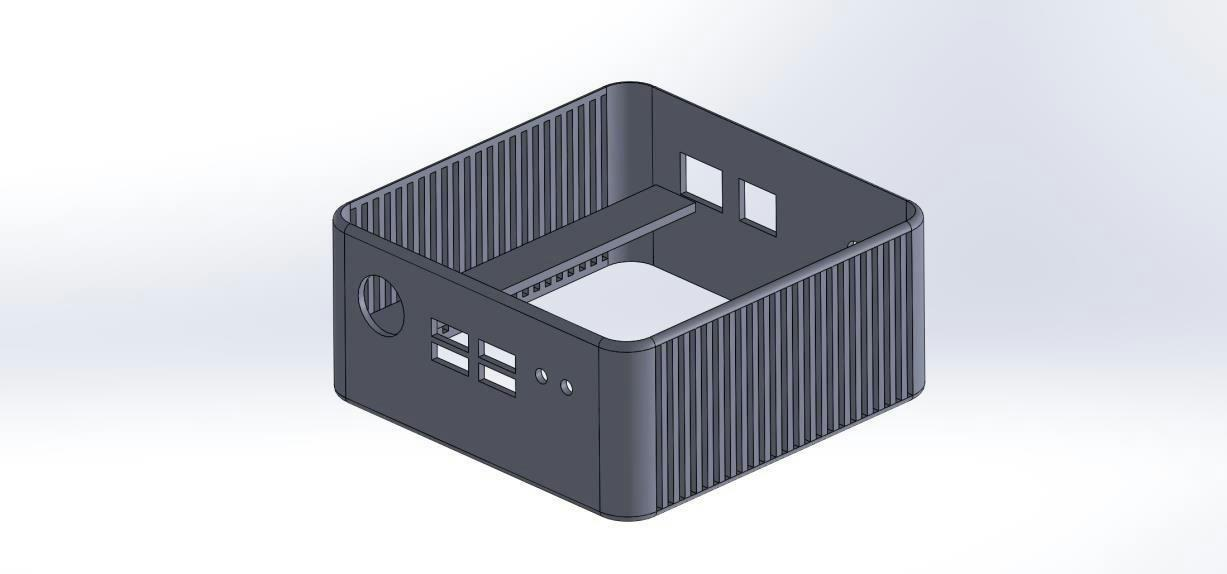
\includegraphics[width=434.16pt,height=202.3pt]{latexImage_55fb47cf62bbcf4c0f0f2bfb8c571345.png}}
\end{picture}
\newpage
\begin{tikzpicture}[overlay]\path(0pt,0pt);\end{tikzpicture}
\begin{picture}(-5,0)(2.5,0)
\put(500.26,-727.616){\fontsize{12}{1}\usefont{T1}{ptm}{m}{n}\selectfont\color{color_29791}22}
\put(511.78,-727.616){\fontsize{12}{1}\usefont{T1}{ptm}{m}{n}\selectfont\color{color_29791} }
\put(63.024,-726.896){\fontsize{9.96}{1}\usefont{T1}{ptm}{m}{n}\selectfont\color{color_29791} }
\put(522.34,-258.37){\fontsize{9.96}{1}\usefont{T1}{ptm}{m}{n}\selectfont\color{color_29791} }
\put(245.45,-274.33){\fontsize{12}{1}\usefont{T1}{ptm}{b}{n}\selectfont\color{color_29791}圖}
\put(257.45,-274.33){\fontsize{12}{1}\usefont{T1}{ptm}{b}{n}\selectfont\color{color_29791} }
\put(260.45,-274.33){\fontsize{12}{1}\usefont{T1}{ptm}{b}{n}\selectfont\color{color_29791}15 B}
\put(283.49,-274.33){\fontsize{12}{1}\usefont{T1}{ptm}{b}{n}\selectfont\color{color_29791} }
\put(286.37,-274.33){\fontsize{12}{1}\usefont{T1}{ptm}{b}{n}\selectfont\color{color_29791}和}
\put(298.49,-274.33){\fontsize{12}{1}\usefont{T1}{ptm}{b}{n}\selectfont\color{color_29791} }
\put(301.49,-274.33){\fontsize{12}{1}\usefont{T1}{ptm}{b}{n}\selectfont\color{color_29791}C}
\put(310.15,-274.33){\fontsize{12}{1}\usefont{T1}{ptm}{b}{n}\selectfont\color{color_29791} }
\put(313.03,-274.33){\fontsize{12}{1}\usefont{T1}{ptm}{b}{n}\selectfont\color{color_29791}部分}
\put(336.55,-274.33){\fontsize{12}{1}\usefont{T1}{ptm}{b}{n}\selectfont\color{color_29791} }
\put(105.38,-312.37){\fontsize{12.81913}{1}\usefont{T1}{ptm}{b}{n}\selectfont\color{color_29791}4.}
\put(114.9648,-312.37){\fontsize{12.81913}{1}\usefont{T1}{ptm}{b}{n}\selectfont\color{color_29791}1}
\put(121.4307,-312.37){\fontsize{12.81913}{1}\usefont{T1}{ptm}{b}{n}\selectfont\color{color_29791}.}
\put(124.5495,-312.37){\fontsize{12.81913}{1}\usefont{T1}{ptm}{b}{n}\selectfont\color{color_29791}3}
\put(131.0154,-312.37){\fontsize{12.81913}{1}\usefont{T1}{ptm}{b}{n}\selectfont\color{color_29791}.}
\put(134.3,-312.37){\fontsize{12.83539}{1}\usefont{T1}{ptm}{b}{n}\selectfont\color{color_29791} }
\put(137.66,-312.37){\fontsize{12.96}{1}\usefont{T1}{ptm}{b}{n}\selectfont\color{color_29791}模具}
\put(163.1,-312.37){\fontsize{12.96}{1}\usefont{T1}{ptm}{b}{n}\selectfont\color{color_29791} }
\put(82.944,-340.69){\fontsize{12}{1}\usefont{T1}{ptm}{m}{n}\selectfont\color{color_29791}理想情況下,所有模具}
\put(203.052,-340.69){\fontsize{12}{1}\usefont{T1}{ptm}{m}{n}\selectfont\color{color_29791}都應由鋼製成,以延長}
\put(323.16,-340.69){\fontsize{12}{1}\usefont{T1}{ptm}{m}{n}\selectfont\color{color_29791}模具的使用壽命和產品}
\put(443.268,-340.69){\fontsize{12}{1}\usefont{T1}{ptm}{m}{n}\selectfont\color{color_29791}品質。話雖}
\put(69.384,-358.57){\fontsize{12}{1}\usefont{T1}{ptm}{m}{n}\selectfont\color{color_29791}如此,}
\put(105.492,-358.57){\fontsize{12}{1}\usefont{T1}{ptm}{m}{n}\selectfont\color{color_29791}為所}
\put(129.6,-358.57){\fontsize{12}{1}\usefont{T1}{ptm}{m}{n}\selectfont\color{color_29791}有零}
\put(153.708,-358.57){\fontsize{12}{1}\usefont{T1}{ptm}{m}{n}\selectfont\color{color_29791}件選}
\put(177.816,-358.57){\fontsize{12}{1}\usefont{T1}{ptm}{m}{n}\selectfont\color{color_29791}擇}
\put(189.924,-358.57){\fontsize{12}{1}\usefont{T1}{ptm}{m}{n}\selectfont\color{color_29791}的注塑}
\put(226.032,-358.57){\fontsize{12}{1}\usefont{T1}{ptm}{m}{n}\selectfont\color{color_29791}塑膠}
\put(250.14,-358.57){\fontsize{12}{1}\usefont{T1}{ptm}{m}{n}\selectfont\color{color_29791}與壓}
\put(274.248,-358.57){\fontsize{12}{1}\usefont{T1}{ptm}{m}{n}\selectfont\color{color_29791}力無}
\put(298.356,-358.57){\fontsize{12}{1}\usefont{T1}{ptm}{m}{n}\selectfont\color{color_29791}關}
\put(310.464,-358.57){\fontsize{12}{1}\usefont{T1}{ptm}{m}{n}\selectfont\color{color_29791},其形}
\put(346.572,-358.57){\fontsize{12}{1}\usefont{T1}{ptm}{m}{n}\selectfont\color{color_29791}式也}
\put(370.68,-358.57){\fontsize{12}{1}\usefont{T1}{ptm}{m}{n}\selectfont\color{color_29791}不那}
\put(394.788,-358.57){\fontsize{12}{1}\usefont{T1}{ptm}{m}{n}\selectfont\color{color_29791}麼複}
\put(418.896,-358.57){\fontsize{12}{1}\usefont{T1}{ptm}{m}{n}\selectfont\color{color_29791}雜}
\put(431.004,-358.57){\fontsize{12}{1}\usefont{T1}{ptm}{m}{n}\selectfont\color{color_29791},因此}
\put(467.112,-358.57){\fontsize{12}{1}\usefont{T1}{ptm}{m}{n}\selectfont\color{color_29791}假設用}
\put(69.384,-376.45){\fontsize{12}{1}\usefont{T1}{ptm}{m}{n}\selectfont\color{color_29791}精密}
\put(92.66,-376.45){\fontsize{12}{1}\usefont{T1}{ptm}{m}{n}\selectfont\color{color_29791} }
\put(98.3,-376.45){\fontsize{12}{1}\usefont{T1}{ptm}{m}{n}\selectfont\color{color_29791}C}
\put(106.328,-376.45){\fontsize{12}{1}\usefont{T1}{ptm}{m}{n}\selectfont\color{color_29791}NC }
\put(126.02,-376.45){\fontsize{12}{1}\usefont{T1}{ptm}{m}{n}\selectfont\color{color_29791}加工製成的}
\put(185.9,-376.45){\fontsize{12}{1}\usefont{T1}{ptm}{m}{n}\selectfont\color{color_29791}鋁模具應該足以生產上述零件。}
\put(353.95,-376.45){\fontsize{12}{1}\usefont{T1}{ptm}{m}{n}\selectfont\color{color_29791} }
\put(63.024,-394.81){\fontsize{12}{1}\usefont{T1}{ptm}{m}{n}\selectfont\color{color_29791} }
\put(82.944,-410.43){\fontsize{12}{1}\usefont{T1}{ptm}{m}{n}\selectfont\color{color_29791}還假設所有模具都足夠簡單,可以使用}
\put(286.97,-410.43){\fontsize{12}{1}\usefont{T1}{ptm}{m}{n}\selectfont\color{color_29791}3}
\put(292.97,-410.43){\fontsize{12}{1}\usefont{T1}{ptm}{m}{n}\selectfont\color{color_29791}D}
\put(301.61,-410.43){\fontsize{12}{1}\usefont{T1}{ptm}{m}{n}\selectfont\color{color_29791}列印進行原型設計。雖然這並不總是正}
\put(69.384,-428.31){\fontsize{12}{1}\usefont{T1}{ptm}{m}{n}\selectfont\color{color_29791}確}
\put(81.384,-428.31){\fontsize{12}{1}\usefont{T1}{ptm}{m}{n}\selectfont\color{color_29791}的}
\put(93.38,-428.31){\fontsize{12}{1}\usefont{T1}{ptm}{m}{n}\selectfont\color{color_29791},但對於這個模擬來說,它被確定為足夠的代表性。這些原型中使用的材料類}
\put(69.384,-446.19){\fontsize{12}{1}\usefont{T1}{ptm}{m}{n}\selectfont\color{color_29791}型是使用}
\put(117.38,-446.19){\fontsize{12}{1}\usefont{T1}{ptm}{m}{n}\selectfont\color{color_29791} }
\put(280.25,-446.19){\fontsize{12}{1}\usefont{T1}{ptm}{m}{n}\selectfont\color{color_29791}S}
\put(287.09,-446.19){\fontsize{12}{1}\usefont{T1}{ptm}{m}{n}\selectfont\color{color_29791}L}
\put(294.17,-446.19){\fontsize{12}{1}\usefont{T1}{ptm}{m}{n}\selectfont\color{color_29791}A}
\put(302.81,-446.19){\fontsize{12}{1}\usefont{T1}{ptm}{m}{n}\selectfont\color{color_29791} }
\put(465.1,-446.19){\fontsize{12}{1}\usefont{T1}{ptm}{m}{n}\selectfont\color{color_29791}3}
\put(470.98,-446.19){\fontsize{12}{1}\usefont{T1}{ptm}{m}{n}\selectfont\color{color_29791}D}
\put(479.5,-446.19){\fontsize{12}{1}\usefont{T1}{ptm}{m}{n}\selectfont\color{color_29791}P}
\put(486.1,-446.19){\fontsize{12}{1}\usefont{T1}{ptm}{m}{n}\selectfont\color{color_29791}r}
\put(489.94,-446.19){\fontsize{12}{1}\usefont{T1}{ptm}{m}{n}\selectfont\color{color_29791}i}
\put(493.18,-446.19){\fontsize{12}{1}\usefont{T1}{ptm}{m}{n}\selectfont\color{color_29791}n}
\put(499.06,-446.19){\fontsize{12}{1}\usefont{T1}{ptm}{m}{n}\selectfont\color{color_29791}t}
\put(502.3,-446.19){\fontsize{12}{1}\usefont{T1}{ptm}{m}{n}\selectfont\color{color_29791}e}
\put(507.46,-446.19){\fontsize{12}{1}\usefont{T1}{ptm}{m}{n}\selectfont\color{color_29791}r}
\put(69.384,-464.07){\fontsize{12}{1}\usefont{T1}{ptm}{m}{n}\selectfont\color{color_29791}固化的高溫退}
\put(141.38,-464.07){\fontsize{12}{1}\usefont{T1}{ptm}{m}{n}\selectfont\color{color_29791}膠}
\put(153.38,-464.07){\fontsize{12}{1}\usefont{T1}{ptm}{m}{n}\selectfont\color{color_29791}。此外,在生產過程中,模具將被視為要開發的主要物理方}
\put(465.46,-464.07){\fontsize{12}{1}\usefont{T1}{ptm}{m}{n}\selectfont\color{color_29791}面}
\put(477.46,-464.07){\fontsize{12}{1}\usefont{T1}{ptm}{m}{n}\selectfont\color{color_29791},因}
\put(69.384,-482.07){\fontsize{12}{1}\usefont{T1}{ptm}{m}{n}\selectfont\color{color_29791}為它直接影響生}
\put(153.38,-482.07){\fontsize{12}{1}\usefont{T1}{ptm}{m}{n}\selectfont\color{color_29791}產}
\put(165.38,-482.07){\fontsize{12}{1}\usefont{T1}{ptm}{m}{n}\selectfont\color{color_29791},並且可以在內部生產並像產品一樣進行跟}
\put(393.43,-482.07){\fontsize{12}{1}\usefont{T1}{ptm}{m}{n}\selectfont\color{color_29791}蹤}
\put(405.43,-482.07){\fontsize{12}{1}\usefont{T1}{ptm}{m}{n}\selectfont\color{color_29791}。}
\put(417.43,-482.07){\fontsize{12}{1}\usefont{T1}{ptm}{m}{n}\selectfont\color{color_29791} }
\put(63.024,-510.03){\fontsize{12}{1}\usefont{T1}{ptm}{m}{n}\selectfont\color{color_29791} }
\put(87.38,-531.27){\fontsize{14.04}{1}\usefont{T1}{ptm}{b}{n}\selectfont\color{color_29791}4}
\put(94.44212,-531.27){\fontsize{14.04}{1}\usefont{T1}{ptm}{b}{n}\selectfont\color{color_29791}.2.}
\put(108.38,-531.27){\fontsize{14.04}{1}\usefont{T1}{ptm}{b}{n}\selectfont\color{color_29791} }
\put(111.74,-531.27){\fontsize{14.04}{1}\usefont{T1}{ptm}{b}{n}\selectfont\color{color_29791}模}
\put(125.6536,-531.27){\fontsize{14.04}{1}\usefont{T1}{ptm}{b}{n}\selectfont\color{color_29791}擬}
\put(139.455,-531.27){\fontsize{14.04}{1}\usefont{T1}{ptm}{b}{n}\selectfont\color{color_29791}過}
\put(153.3686,-531.27){\fontsize{14.04}{1}\usefont{T1}{ptm}{b}{n}\selectfont\color{color_29791}程}
\put(167.1699,-531.27){\fontsize{14.04}{1}\usefont{T1}{ptm}{b}{n}\selectfont\color{color_29791}中}
\put(181.0835,-531.27){\fontsize{14.04}{1}\usefont{T1}{ptm}{b}{n}\selectfont\color{color_29791}分}
\put(194.8849,-531.27){\fontsize{14.04}{1}\usefont{T1}{ptm}{b}{n}\selectfont\color{color_29791}析}
\put(208.6862,-531.27){\fontsize{14.04}{1}\usefont{T1}{ptm}{b}{n}\selectfont\color{color_29791}的}
\put(222.4875,-531.27){\fontsize{14.04}{1}\usefont{T1}{ptm}{b}{n}\selectfont\color{color_29791}內}
\put(236.4011,-531.27){\fontsize{14.04}{1}\usefont{T1}{ptm}{b}{n}\selectfont\color{color_29791}容}
\put(250.25,-531.27){\fontsize{14.04}{1}\usefont{T1}{ptm}{b}{n}\selectfont\color{color_29791} }
\put(82.944,-565.11){\fontsize{12}{1}\usefont{T1}{ptm}{m}{n}\selectfont\color{color_29791}考慮到}
\put(118.94,-565.11){\fontsize{12}{1}\usefont{T1}{ptm}{m}{n}\selectfont\color{color_29791}圖}
\put(130.46,-565.11){\fontsize{12}{1}\usefont{T1}{ptm}{m}{n}\selectfont\color{color_29791} }
\put(149.66,-565.11){\fontsize{12}{1}\usefont{T1}{ptm}{m}{n}\selectfont\color{color_29791}9}
\put(155.18,-565.11){\fontsize{12}{1}\usefont{T1}{ptm}{m}{n}\selectfont\color{color_29791} }
\put(174.38,-565.11){\fontsize{12}{1}\usefont{T1}{ptm}{m}{n}\selectfont\color{color_29791}所示的圖表,以及}
\put(270.41,-565.11){\fontsize{12}{1}\usefont{T1}{ptm}{m}{n}\selectfont\color{color_29791}第}
\put(281.93,-565.11){\fontsize{12}{1}\usefont{T1}{ptm}{m}{n}\selectfont\color{color_29791} }
\put(301.13,-565.11){\fontsize{12}{1}\usefont{T1}{ptm}{m}{n}\selectfont\color{color_29791}3.1}
\put(315.43,-565.11){\fontsize{12}{1}\usefont{T1}{ptm}{m}{n}\selectfont\color{color_29791} }
\put(334.87,-565.11){\fontsize{12}{1}\usefont{T1}{ptm}{m}{n}\selectfont\color{color_29791}節中描述}
\put(382.87,-565.11){\fontsize{12}{1}\usefont{T1}{ptm}{m}{n}\selectfont\color{color_29791}的}
\put(394.39,-565.11){\fontsize{12}{1}\usefont{T1}{ptm}{m}{n}\selectfont\color{color_29791} }
\put(413.59,-565.11){\fontsize{12}{1}\usefont{T1}{ptm}{m}{n}\selectfont\color{color_29791}P}
\put(420.07,-565.11){\fontsize{12}{1}\usefont{T1}{ptm}{m}{n}\selectfont\color{color_29791}L}
\put(427.15,-565.11){\fontsize{12}{1}\usefont{T1}{ptm}{m}{n}\selectfont\color{color_29791}M}
\put(437.47,-565.11){\fontsize{12}{1}\usefont{T1}{ptm}{m}{n}\selectfont\color{color_29791} }
\put(457.18,-565.11){\fontsize{12}{1}\usefont{T1}{ptm}{m}{n}\selectfont\color{color_29791}和}
\put(468.7,-565.11){\fontsize{12}{1}\usefont{T1}{ptm}{m}{n}\selectfont\color{color_29791} }
\put(487.9,-565.11){\fontsize{12}{1}\usefont{T1}{ptm}{m}{n}\selectfont\color{color_29791}M}
\put(498.34,-565.11){\fontsize{12}{1}\usefont{T1}{ptm}{m}{n}\selectfont\color{color_29791}E}
\put(505.42,-565.11){\fontsize{12}{1}\usefont{T1}{ptm}{m}{n}\selectfont\color{color_29791}S}
\put(511.78,-565.11){\fontsize{12}{1}\usefont{T1}{ptm}{m}{n}\selectfont\color{color_29791} }
\put(69.384,-583.14){\fontsize{12}{1}\usefont{T1}{ptm}{m}{n}\selectfont\color{color_29791}成}
\put(81.144,-583.14){\fontsize{12}{1}\usefont{T1}{ptm}{m}{n}\selectfont\color{color_29791}功}
\put(92.90401,-583.14){\fontsize{12}{1}\usefont{T1}{ptm}{m}{n}\selectfont\color{color_29791}集}
\put(104.664,-583.14){\fontsize{12}{1}\usefont{T1}{ptm}{m}{n}\selectfont\color{color_29791}成}
\put(116.544,-583.14){\fontsize{12}{1}\usefont{T1}{ptm}{m}{n}\selectfont\color{color_29791}的}
\put(128.304,-583.14){\fontsize{12}{1}\usefont{T1}{ptm}{m}{n}\selectfont\color{color_29791}主}
\put(140.064,-583.14){\fontsize{12}{1}\usefont{T1}{ptm}{m}{n}\selectfont\color{color_29791}要}
\put(151.944,-583.14){\fontsize{12}{1}\usefont{T1}{ptm}{m}{n}\selectfont\color{color_29791}方}
\put(163.704,-583.14){\fontsize{12}{1}\usefont{T1}{ptm}{m}{n}\selectfont\color{color_29791}面}
\put(175.464,-583.14){\fontsize{12}{1}\usefont{T1}{ptm}{m}{n}\selectfont\color{color_29791},}
\put(187.344,-583.14){\fontsize{12}{1}\usefont{T1}{ptm}{m}{n}\selectfont\color{color_29791}本}
\put(199.104,-583.14){\fontsize{12}{1}\usefont{T1}{ptm}{m}{n}\selectfont\color{color_29791}實}
\put(210.864,-583.14){\fontsize{12}{1}\usefont{T1}{ptm}{m}{n}\selectfont\color{color_29791}驗}
\put(222.624,-583.14){\fontsize{12}{1}\usefont{T1}{ptm}{m}{n}\selectfont\color{color_29791}旨}
\put(234.504,-583.14){\fontsize{12}{1}\usefont{T1}{ptm}{m}{n}\selectfont\color{color_29791}在}
\put(246.264,-583.14){\fontsize{12}{1}\usefont{T1}{ptm}{m}{n}\selectfont\color{color_29791}對}
\put(258.024,-583.14){\fontsize{12}{1}\usefont{T1}{ptm}{m}{n}\selectfont\color{color_29791}表}
\put(269.93,-583.14){\fontsize{12}{1}\usefont{T1}{ptm}{m}{n}\selectfont\color{color_29791} }
\put(275.69,-583.14){\fontsize{12}{1}\usefont{T1}{ptm}{m}{n}\selectfont\color{color_29791}1}
\put(281.69,-583.14){\fontsize{12}{1}\usefont{T1}{ptm}{m}{n}\selectfont\color{color_29791} }
\put(284.69,-583.14){\fontsize{12}{1}\usefont{T1}{ptm}{m}{n}\selectfont\color{color_29791}中的}
\put(308.57,-583.14){\fontsize{12}{1}\usefont{T1}{ptm}{m}{n}\selectfont\color{color_29791}以下相}
\put(344.45,-583.14){\fontsize{12}{1}\usefont{T1}{ptm}{m}{n}\selectfont\color{color_29791}關問題}
\put(380.33,-583.14){\fontsize{12}{1}\usefont{T1}{ptm}{m}{n}\selectfont\color{color_29791}進行}
\put(404.21,-583.14){\fontsize{12}{1}\usefont{T1}{ptm}{m}{n}\selectfont\color{color_29791}評論}
\put(428.09,-583.14){\fontsize{12}{1}\usefont{T1}{ptm}{m}{n}\selectfont\color{color_29791}。}
\put(440.14,-583.14){\fontsize{12}{1}\usefont{T1}{ptm}{m}{n}\selectfont\color{color_29791} }
\put(291.53,-615.3){\fontsize{12}{1}\usefont{T1}{ptm}{b}{n}\selectfont\color{color_29791}表}
\put(303.53,-615.3){\fontsize{12}{1}\usefont{T1}{ptm}{b}{n}\selectfont\color{color_29791}1}
\put(309.55,-615.3){\fontsize{12}{1}\usefont{T1}{ptm}{b}{n}\selectfont\color{color_29791} }
\put(312.67,-615.3){\fontsize{12}{1}\usefont{T1}{ptm}{b}{n}\selectfont\color{color_29791}需回答的問題摘要}
\put(407.83,-615.3){\fontsize{12}{1}\usefont{T1}{ptm}{b}{n}\selectfont\color{color_29791} }
\end{picture}
\begin{tikzpicture}[overlay]
\path(0pt,0pt);
\filldraw[color_213730][even odd rule]
(70.464pt, -636.9pt) -- (209.684pt, -636.9pt)
 -- (209.684pt, -636.9pt)
 -- (209.684pt, -620.7pt)
 -- (209.684pt, -620.7pt)
 -- (70.464pt, -620.7pt) -- cycle
;
\begin{scope}
\clip
(70.464pt, -636.9pt) -- (209.684pt, -636.9pt)
 -- (209.684pt, -636.9pt)
 -- (209.684pt, -620.7pt)
 -- (209.684pt, -620.7pt)
 -- (70.464pt, -620.7pt) -- cycle
;
\filldraw[color_213730][even odd rule]
(70.464pt, -635.94pt) -- (209.684pt, -635.94pt)
 -- (209.684pt, -635.94pt)
 -- (209.684pt, -620.7pt)
 -- (209.684pt, -620.7pt)
 -- (70.464pt, -620.7pt) -- cycle
;
\begin{scope}
\clip
(70.464pt, -636.9pt) -- (209.684pt, -636.9pt)
 -- (209.684pt, -636.9pt)
 -- (209.684pt, -620.7pt)
 -- (209.684pt, -620.7pt)
 -- (70.464pt, -620.7pt) -- cycle
;
\end{scope}
\end{scope}
\end{tikzpicture}
\begin{picture}(-5,0)(2.5,0)
\put(75.864,-632.94){\fontsize{9.96}{1}\usefont{T1}{ptm}{b}{n}\selectfont\color{color_29791}類別}
\put(95.42,-632.94){\fontsize{9.96}{1}\usefont{T1}{ptm}{b}{n}\selectfont\color{color_29791} }
\end{picture}
\begin{tikzpicture}[overlay]
\path(0pt,0pt);
\filldraw[color_241678][even odd rule]
(209.69pt, -636.9pt) -- (511.54pt, -636.9pt)
 -- (511.54pt, -636.9pt)
 -- (511.54pt, -620.7pt)
 -- (511.54pt, -620.7pt)
 -- (209.69pt, -620.7pt) -- cycle
;
\begin{scope}
\clip
(209.69pt, -636.9pt) -- (511.54pt, -636.9pt)
 -- (511.54pt, -636.9pt)
 -- (511.54pt, -620.7pt)
 -- (511.54pt, -620.7pt)
 -- (209.69pt, -620.7pt) -- cycle
;
\filldraw[color_241678][even odd rule]
(209.69pt, -635.94pt) -- (511.54pt, -635.94pt)
 -- (511.54pt, -635.94pt)
 -- (511.54pt, -620.7pt)
 -- (511.54pt, -620.7pt)
 -- (209.69pt, -620.7pt) -- cycle
;
\begin{scope}
\clip
(209.69pt, -636.9pt) -- (511.54pt, -636.9pt)
 -- (511.54pt, -636.9pt)
 -- (511.54pt, -620.7pt)
 -- (511.54pt, -620.7pt)
 -- (209.69pt, -620.7pt) -- cycle
;
\end{scope}
\end{scope}
\end{tikzpicture}
\begin{picture}(-5,0)(2.5,0)
\put(215.09,-632.94){\fontsize{9.96}{1}\usefont{T1}{ptm}{b}{n}\selectfont\color{color_29791}問題}
\put(234.65,-632.94){\fontsize{9.96}{1}\usefont{T1}{ptm}{b}{n}\selectfont\color{color_29791} }
\end{picture}
\begin{tikzpicture}[overlay]
\path(0pt,0pt);
\filldraw[color_269104][even odd rule]
(70.464pt, -669.42pt) -- (209.444pt, -669.42pt)
 -- (209.444pt, -669.42pt)
 -- (209.444pt, -636.9pt)
 -- (209.444pt, -636.9pt)
 -- (70.464pt, -636.9pt) -- cycle
;
\begin{scope}
\clip
(70.464pt, -669.42pt) -- (209.444pt, -669.42pt)
 -- (209.444pt, -669.42pt)
 -- (209.444pt, -636.9pt)
 -- (209.444pt, -636.9pt)
 -- (70.464pt, -636.9pt) -- cycle
;
\filldraw[color_269104][even odd rule]
(70.464pt, -650.82pt) -- (209.444pt, -650.82pt)
 -- (209.444pt, -650.82pt)
 -- (209.444pt, -636.9pt)
 -- (209.444pt, -636.9pt)
 -- (70.464pt, -636.9pt) -- cycle
;
\begin{scope}
\clip
(70.464pt, -669.42pt) -- (209.444pt, -669.42pt)
 -- (209.444pt, -669.42pt)
 -- (209.444pt, -636.9pt)
 -- (209.444pt, -636.9pt)
 -- (70.464pt, -636.9pt) -- cycle
;
\end{scope}
\end{scope}
\end{tikzpicture}
\begin{picture}(-5,0)(2.5,0)
\put(90.02,-647.94){\fontsize{9.96}{1}\usefont{T1}{ptm}{m}{n}\selectfont\color{color_29791}該軟體如何處理專案?}
\put(188.57,-647.94){\fontsize{9.96}{1}\usefont{T1}{ptm}{m}{n}\selectfont\color{color_29791} }
\end{picture}
\begin{tikzpicture}[overlay]
\path(0pt,0pt);
\filldraw[color_269104][even odd rule]
(210.05pt, -652.74pt) -- (511.54pt, -652.74pt)
 -- (511.54pt, -652.74pt)
 -- (511.54pt, -636.9pt)
 -- (511.54pt, -636.9pt)
 -- (210.05pt, -636.9pt) -- cycle
;
\begin{scope}
\clip
(210.05pt, -652.74pt) -- (511.54pt, -652.74pt)
 -- (511.54pt, -652.74pt)
 -- (511.54pt, -636.9pt)
 -- (511.54pt, -636.9pt)
 -- (210.05pt, -636.9pt) -- cycle
;
\filldraw[color_269104][even odd rule]
(210.05pt, -650.82pt) -- (511.54pt, -650.82pt)
 -- (511.54pt, -650.82pt)
 -- (511.54pt, -636.9pt)
 -- (511.54pt, -636.9pt)
 -- (210.05pt, -636.9pt) -- cycle
;
\begin{scope}
\clip
(210.05pt, -652.74pt) -- (511.54pt, -652.74pt)
 -- (511.54pt, -652.74pt)
 -- (511.54pt, -636.9pt)
 -- (511.54pt, -636.9pt)
 -- (210.05pt, -636.9pt) -- cycle
;
\end{scope}
\end{scope}
\end{tikzpicture}
\begin{picture}(-5,0)(2.5,0)
\put(215.21,-647.94){\fontsize{9.96}{1}\usefont{T1}{ptm}{m}{n}\selectfont\color{color_29791}是否代表了產品生命週期的}
\put(333.3996,-647.94){\fontsize{9.96}{1}\usefont{T1}{ptm}{m}{n}\selectfont\color{color_29791}所有方面?}
\put(382.63,-647.94){\fontsize{9.96}{1}\usefont{T1}{ptm}{m}{n}\selectfont\color{color_29791} }
\end{picture}
\begin{tikzpicture}[overlay]
\path(0pt,0pt);
\filldraw[color_29791][even odd rule]
(209.57pt, -652.74pt) -- (210.05pt, -652.74pt)
 -- (210.05pt, -652.74pt)
 -- (210.05pt, -636.9pt)
 -- (210.05pt, -636.9pt)
 -- (209.57pt, -636.9pt) -- cycle
;
\begin{scope}
\clip
(210.05pt, -669.42pt) -- (511.54pt, -669.42pt)
 -- (511.54pt, -669.42pt)
 -- (511.54pt, -653.22pt)
 -- (511.54pt, -653.22pt)
 -- (210.05pt, -653.22pt) -- cycle
;
\begin{scope}
\clip
(210.05pt, -669.42pt) -- (511.54pt, -669.42pt)
 -- (511.54pt, -669.42pt)
 -- (511.54pt, -653.22pt)
 -- (511.54pt, -653.22pt)
 -- (210.05pt, -653.22pt) -- cycle
;
\end{scope}
\end{scope}
\end{tikzpicture}
\begin{picture}(-5,0)(2.5,0)
\put(215.21,-664.02){\fontsize{9.96}{1}\usefont{T1}{ptm}{m}{n}\selectfont\color{color_29791}這些專案中的每一個都表現}
\put(333.3996,-664.02){\fontsize{9.96}{1}\usefont{T1}{ptm}{m}{n}\selectfont\color{color_29791}得如何?}
\put(372.79,-664.02){\fontsize{9.96}{1}\usefont{T1}{ptm}{m}{n}\selectfont\color{color_29791} }
\end{picture}
\begin{tikzpicture}[overlay]
\path(0pt,0pt);
\filldraw[color_29791][even odd rule]
(209.57pt, -653.22pt) -- (210.05pt, -653.22pt)
 -- (210.05pt, -653.22pt)
 -- (210.05pt, -652.74pt)
 -- (210.05pt, -652.74pt)
 -- (209.57pt, -652.74pt) -- cycle
;
\filldraw[color_29791][even odd rule]
(209.57pt, -669.42pt) -- (210.05pt, -669.42pt)
 -- (210.05pt, -669.42pt)
 -- (210.05pt, -653.22pt)
 -- (210.05pt, -653.22pt)
 -- (209.57pt, -653.22pt) -- cycle
;
\filldraw[color_269104][even odd rule]
(70.464pt, -702.416pt) -- (209.444pt, -702.416pt)
 -- (209.444pt, -702.416pt)
 -- (209.444pt, -669.896pt)
 -- (209.444pt, -669.896pt)
 -- (70.464pt, -669.896pt) -- cycle
;
\begin{scope}
\clip
(70.464pt, -702.416pt) -- (209.444pt, -702.416pt)
 -- (209.444pt, -702.416pt)
 -- (209.444pt, -669.896pt)
 -- (209.444pt, -669.896pt)
 -- (70.464pt, -669.896pt) -- cycle
;
\filldraw[color_269104][even odd rule]
(70.464pt, -685.136pt) -- (209.444pt, -685.136pt)
 -- (209.444pt, -685.136pt)
 -- (209.444pt, -669.896pt)
 -- (209.444pt, -669.896pt)
 -- (70.464pt, -669.896pt) -- cycle
;
\begin{scope}
\clip
(70.464pt, -702.416pt) -- (209.444pt, -702.416pt)
 -- (209.444pt, -702.416pt)
 -- (209.444pt, -669.896pt)
 -- (209.444pt, -669.896pt)
 -- (70.464pt, -669.896pt) -- cycle
;
\end{scope}
\end{scope}
\end{tikzpicture}
\begin{picture}(-5,0)(2.5,0)
\put(75.864,-680.94){\fontsize{9.96}{1}\usefont{T1}{ptm}{m}{n}\selectfont\color{color_29791}創}
\put(86.53116,-680.94){\fontsize{9.96}{1}\usefont{T1}{ptm}{m}{n}\selectfont\color{color_29791}造}
\put(97.31784,-680.94){\fontsize{9.96}{1}\usefont{T1}{ptm}{m}{n}\selectfont\color{color_29791}一}
\put(107.985,-680.94){\fontsize{9.96}{1}\usefont{T1}{ptm}{m}{n}\selectfont\color{color_29791}個}
\put(118.7717,-680.94){\fontsize{9.96}{1}\usefont{T1}{ptm}{m}{n}\selectfont\color{color_29791}全}
\put(129.5584,-680.94){\fontsize{9.96}{1}\usefont{T1}{ptm}{m}{n}\selectfont\color{color_29791}新}
\put(140.2255,-680.94){\fontsize{9.96}{1}\usefont{T1}{ptm}{m}{n}\selectfont\color{color_29791}的}
\put(151.0122,-680.94){\fontsize{9.96}{1}\usefont{T1}{ptm}{m}{n}\selectfont\color{color_29791}產}
\put(161.6794,-680.94){\fontsize{9.96}{1}\usefont{T1}{ptm}{m}{n}\selectfont\color{color_29791}品}
\put(172.466,-680.94){\fontsize{9.96}{1}\usefont{T1}{ptm}{m}{n}\selectfont\color{color_29791}有}
\put(183.1332,-680.94){\fontsize{9.96}{1}\usefont{T1}{ptm}{m}{n}\selectfont\color{color_29791}多}
\put(193.9199,-680.94){\fontsize{9.96}{1}\usefont{T1}{ptm}{m}{n}\selectfont\color{color_29791}容}
\end{picture}
\begin{tikzpicture}[overlay]
\path(0pt,0pt);
\begin{scope}
\clip
(70.464pt, -702.416pt) -- (209.444pt, -702.416pt)
 -- (209.444pt, -702.416pt)
 -- (209.444pt, -669.896pt)
 -- (209.444pt, -669.896pt)
 -- (70.464pt, -669.896pt) -- cycle
;
\filldraw[color_269104][even odd rule]
(70.464pt, -699.416pt) -- (209.444pt, -699.416pt)
 -- (209.444pt, -699.416pt)
 -- (209.444pt, -685.136pt)
 -- (209.444pt, -685.136pt)
 -- (70.464pt, -685.136pt) -- cycle
;
\begin{scope}
\clip
(70.464pt, -702.416pt) -- (209.444pt, -702.416pt)
 -- (209.444pt, -702.416pt)
 -- (209.444pt, -669.896pt)
 -- (209.444pt, -669.896pt)
 -- (70.464pt, -669.896pt) -- cycle
;
\end{scope}
\end{scope}
\end{tikzpicture}
\begin{picture}(-5,0)(2.5,0)
\put(75.864,-695.216){\fontsize{9.96}{1}\usefont{T1}{ptm}{m}{n}\selectfont\color{color_29791}易?}
\put(95.3,-695.216){\fontsize{9.96}{1}\usefont{T1}{ptm}{m}{n}\selectfont\color{color_29791} }
\end{picture}
\begin{tikzpicture}[overlay]
\path(0pt,0pt);
\filldraw[color_269104][even odd rule]
(210.05pt, -686.336pt) -- (511.54pt, -686.336pt)
 -- (511.54pt, -686.336pt)
 -- (511.54pt, -669.896pt)
 -- (511.54pt, -669.896pt)
 -- (210.05pt, -669.896pt) -- cycle
;
\begin{scope}
\clip
(210.05pt, -686.336pt) -- (511.54pt, -686.336pt)
 -- (511.54pt, -686.336pt)
 -- (511.54pt, -669.896pt)
 -- (511.54pt, -669.896pt)
 -- (210.05pt, -669.896pt) -- cycle
;
\filldraw[color_269104][even odd rule]
(210.05pt, -683.816pt) -- (511.54pt, -683.816pt)
 -- (511.54pt, -683.816pt)
 -- (511.54pt, -669.896pt)
 -- (511.54pt, -669.896pt)
 -- (210.05pt, -669.896pt) -- cycle
;
\begin{scope}
\clip
(210.05pt, -686.336pt) -- (511.54pt, -686.336pt)
 -- (511.54pt, -686.336pt)
 -- (511.54pt, -669.896pt)
 -- (511.54pt, -669.896pt)
 -- (210.05pt, -669.896pt) -- cycle
;
\end{scope}
\end{scope}
\end{tikzpicture}
\begin{picture}(-5,0)(2.5,0)
\put(215.21,-680.94){\fontsize{9.96}{1}\usefont{T1}{ptm}{m}{n}\selectfont\color{color_29791}產}
\put(224.931,-680.94){\fontsize{9.96}{1}\usefont{T1}{ptm}{m}{n}\selectfont\color{color_29791}品}
\put(234.7715,-680.94){\fontsize{9.96}{1}\usefont{T1}{ptm}{m}{n}\selectfont\color{color_29791}的}
\put(244.6119,-680.94){\fontsize{9.96}{1}\usefont{T1}{ptm}{m}{n}\selectfont\color{color_29791}描}
\put(254.3329,-680.94){\fontsize{9.96}{1}\usefont{T1}{ptm}{m}{n}\selectfont\color{color_29791}述}
\put(264.1734,-680.94){\fontsize{9.96}{1}\usefont{T1}{ptm}{m}{n}\selectfont\color{color_29791}方}
\put(274.0139,-680.94){\fontsize{9.96}{1}\usefont{T1}{ptm}{m}{n}\selectfont\color{color_29791}式}
\put(283.85,-680.94){\fontsize{9.96}{1}\usefont{T1}{ptm}{m}{n}\selectfont\color{color_29791} }
\end{picture}
\begin{tikzpicture}[overlay]
\path(0pt,0pt);
\filldraw[color_29791][even odd rule]
(70.464pt, -669.9pt) -- (209.564pt, -669.9pt)
 -- (209.564pt, -669.9pt)
 -- (209.564pt, -669.42pt)
 -- (209.564pt, -669.42pt)
 -- (70.464pt, -669.42pt) -- cycle
;
\filldraw[color_29791][even odd rule]
(209.57pt, -669.9pt) -- (210.05pt, -669.9pt)
 -- (210.05pt, -669.9pt)
 -- (210.05pt, -669.42pt)
 -- (210.05pt, -669.42pt)
 -- (209.57pt, -669.42pt) -- cycle
;
\filldraw[color_29791][even odd rule]
(210.05pt, -669.9pt) -- (511.54pt, -669.9pt)
 -- (511.54pt, -669.9pt)
 -- (511.54pt, -669.42pt)
 -- (511.54pt, -669.42pt)
 -- (210.05pt, -669.42pt) -- cycle
;
\filldraw[color_29791][even odd rule]
(209.57pt, -686.336pt) -- (210.05pt, -686.336pt)
 -- (210.05pt, -686.336pt)
 -- (210.05pt, -669.896pt)
 -- (210.05pt, -669.896pt)
 -- (209.57pt, -669.896pt) -- cycle
;
\begin{scope}
\clip
(210.05pt, -702.416pt) -- (511.54pt, -702.416pt)
 -- (511.54pt, -702.416pt)
 -- (511.54pt, -686.336pt)
 -- (511.54pt, -686.336pt)
 -- (210.05pt, -686.336pt) -- cycle
;
\begin{scope}
\clip
(210.05pt, -702.416pt) -- (511.54pt, -702.416pt)
 -- (511.54pt, -702.416pt)
 -- (511.54pt, -686.336pt)
 -- (511.54pt, -686.336pt)
 -- (210.05pt, -686.336pt) -- cycle
;
\end{scope}
\end{scope}
\end{tikzpicture}
\begin{picture}(-5,0)(2.5,0)
\put(215.21,-697.376){\fontsize{9.96}{1}\usefont{T1}{ptm}{m}{n}\selectfont\color{color_29791}產品如何集成和引用相關文}
\put(333.3996,-697.376){\fontsize{9.96}{1}\usefont{T1}{ptm}{m}{n}\selectfont\color{color_29791}件?}
\put(353.11,-697.376){\fontsize{9.96}{1}\usefont{T1}{ptm}{m}{n}\selectfont\color{color_29791} }
\end{picture}
\begin{tikzpicture}[overlay]
\path(0pt,0pt);
\filldraw[color_29791][even odd rule]
(209.57pt, -702.416pt) -- (210.05pt, -702.416pt)
 -- (210.05pt, -702.416pt)
 -- (210.05pt, -686.336pt)
 -- (210.05pt, -686.336pt)
 -- (209.57pt, -686.336pt) -- cycle
;
\begin{scope}
\clip
(87.9pt, -258.32pt) -- (522.32pt, -258.32pt)
 -- (522.32pt, -258.32pt)
 -- (522.32pt, -61.04004pt)
 -- (522.32pt, -61.04004pt)
 -- (87.9pt, -61.04004pt) -- cycle
;
\end{scope}
\end{tikzpicture}
\begin{picture}(-5,0)(2.5,0)
\put(87.9,-258.35){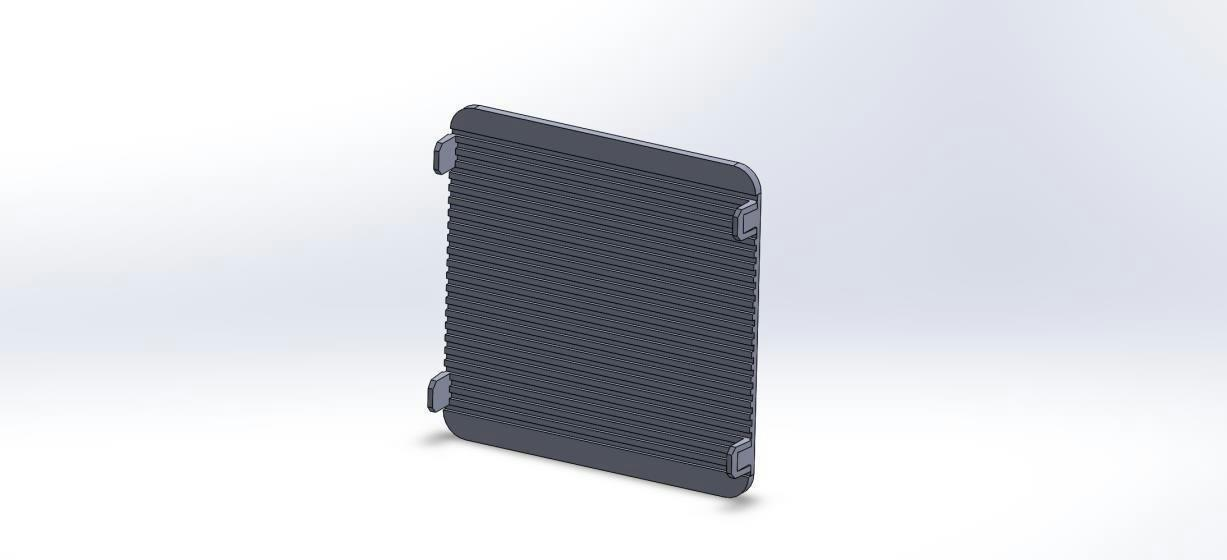
\includegraphics[width=434.42pt,height=197.35pt]{latexImage_c57658e5d81c3b997a07b5139f5a4e23.png}}
\end{picture}
\newpage
\begin{tikzpicture}[overlay]\path(0pt,0pt);\end{tikzpicture}
\begin{picture}(-5,0)(2.5,0)
\put(500.26,-727.616){\fontsize{12}{1}\usefont{T1}{ptm}{m}{n}\selectfont\color{color_29791}23}
\put(511.78,-727.616){\fontsize{12}{1}\usefont{T1}{ptm}{m}{n}\selectfont\color{color_29791} }
\put(63.024,-726.896){\fontsize{9.96}{1}\usefont{T1}{ptm}{m}{n}\selectfont\color{color_29791} }
\end{picture}
\begin{tikzpicture}[overlay]
\path(0pt,0pt);
\filldraw[color_269104][even odd rule]
(70.464pt, -76.41998pt) -- (209.444pt, -76.41998pt)
 -- (209.444pt, -76.41998pt)
 -- (209.444pt, -59.95599pt)
 -- (209.444pt, -59.95599pt)
 -- (70.464pt, -59.95599pt) -- cycle
;
\begin{scope}
\clip
(70.464pt, -76.41998pt) -- (209.444pt, -76.41998pt)
 -- (209.444pt, -76.41998pt)
 -- (209.444pt, -59.95599pt)
 -- (209.444pt, -59.95599pt)
 -- (70.464pt, -59.95599pt) -- cycle
;
\filldraw[color_269104][even odd rule]
(70.464pt, -72.67999pt) -- (209.444pt, -72.67999pt)
 -- (209.444pt, -72.67999pt)
 -- (209.444pt, -59.96002pt)
 -- (209.444pt, -59.96002pt)
 -- (70.464pt, -59.96002pt) -- cycle
;
\begin{scope}
\clip
(70.464pt, -76.41998pt) -- (209.444pt, -76.41998pt)
 -- (209.444pt, -76.41998pt)
 -- (209.444pt, -59.95599pt)
 -- (209.444pt, -59.95599pt)
 -- (70.464pt, -59.95599pt) -- cycle
;
\end{scope}
\end{scope}
\end{tikzpicture}
\begin{picture}(-5,0)(2.5,0)
\put(70.464,-70.15997){\fontsize{11.04}{1}\usefont{T1}{ptm}{m}{n}\selectfont\color{color_29791} }
\end{picture}
\begin{tikzpicture}[overlay]
\path(0pt,0pt);
\filldraw[color_269104][even odd rule]
(209.93pt, -76.41998pt) -- (511.42pt, -76.41998pt)
 -- (511.42pt, -76.41998pt)
 -- (511.42pt, -59.95599pt)
 -- (511.42pt, -59.95599pt)
 -- (209.93pt, -59.95599pt) -- cycle
;
\begin{scope}
\clip
(209.93pt, -76.41998pt) -- (511.42pt, -76.41998pt)
 -- (511.42pt, -76.41998pt)
 -- (511.42pt, -59.95599pt)
 -- (511.42pt, -59.95599pt)
 -- (209.93pt, -59.95599pt) -- cycle
;
\filldraw[color_269104][even odd rule]
(209.93pt, -74.62pt) -- (511.42pt, -74.62pt)
 -- (511.42pt, -74.62pt)
 -- (511.42pt, -59.95599pt)
 -- (511.42pt, -59.95599pt)
 -- (209.93pt, -59.95599pt) -- cycle
;
\begin{scope}
\clip
(209.93pt, -76.41998pt) -- (511.42pt, -76.41998pt)
 -- (511.42pt, -76.41998pt)
 -- (511.42pt, -59.95599pt)
 -- (511.42pt, -59.95599pt)
 -- (209.93pt, -59.95599pt) -- cycle
;
\end{scope}
\end{scope}
\end{tikzpicture}
\begin{picture}(-5,0)(2.5,0)
\put(215.09,-71.71997){\fontsize{9.96}{1}\usefont{T1}{ptm}{m}{n}\selectfont\color{color_29791}改變一個會影響另一個嗎?}
\put(333.31,-71.71997){\fontsize{9.96}{1}\usefont{T1}{ptm}{m}{n}\selectfont\color{color_29791} }
\end{picture}
\begin{tikzpicture}[overlay]
\path(0pt,0pt);
\filldraw[color_29791][even odd rule]
(209.45pt, -76.41998pt) -- (209.93pt, -76.41998pt)
 -- (209.93pt, -76.41998pt)
 -- (209.93pt, -59.95599pt)
 -- (209.93pt, -59.95599pt)
 -- (209.45pt, -59.95599pt) -- cycle
;
\filldraw[color_269104][even odd rule]
(70.464pt, -125.98pt) -- (209.444pt, -125.98pt)
 -- (209.444pt, -125.98pt)
 -- (209.444pt, -77.01996pt)
 -- (209.444pt, -77.01996pt)
 -- (70.464pt, -77.01996pt) -- cycle
;
\begin{scope}
\clip
(70.464pt, -125.98pt) -- (209.444pt, -125.98pt)
 -- (209.444pt, -125.98pt)
 -- (209.444pt, -77.01996pt)
 -- (209.444pt, -77.01996pt)
 -- (70.464pt, -77.01996pt) -- cycle
;
\filldraw[color_269104][even odd rule]
(70.464pt, -92.85999pt) -- (209.444pt, -92.85999pt)
 -- (209.444pt, -92.85999pt)
 -- (209.444pt, -77.01996pt)
 -- (209.444pt, -77.01996pt)
 -- (70.464pt, -77.01996pt) -- cycle
;
\begin{scope}
\clip
(70.464pt, -125.98pt) -- (209.444pt, -125.98pt)
 -- (209.444pt, -125.98pt)
 -- (209.444pt, -77.01996pt)
 -- (209.444pt, -77.01996pt)
 -- (70.464pt, -77.01996pt) -- cycle
;
\end{scope}
\end{scope}
\end{tikzpicture}
\begin{picture}(-5,0)(2.5,0)
\put(90.02,-88.65997){\fontsize{9.96}{1}\usefont{T1}{ptm}{m}{n}\selectfont\color{color_29791}創建一個}
\put(129.9696,-88.65997){\fontsize{9.96}{1}\usefont{T1}{ptm}{m}{n}\selectfont\color{color_29791}全新的}
\put(159.9591,-88.65997){\fontsize{9.96}{1}\usefont{T1}{ptm}{m}{n}\selectfont\color{color_29791}生產流}
\put(189.9487,-88.65997){\fontsize{9.96}{1}\usefont{T1}{ptm}{m}{n}\selectfont\color{color_29791}程}
\end{picture}
\begin{tikzpicture}[overlay]
\path(0pt,0pt);
\begin{scope}
\clip
(70.464pt, -125.98pt) -- (209.444pt, -125.98pt)
 -- (209.444pt, -125.98pt)
 -- (209.444pt, -77.01996pt)
 -- (209.444pt, -77.01996pt)
 -- (70.464pt, -77.01996pt) -- cycle
;
\filldraw[color_269104][even odd rule]
(70.464pt, -107.14pt) -- (209.444pt, -107.14pt)
 -- (209.444pt, -107.14pt)
 -- (209.444pt, -92.85999pt)
 -- (209.444pt, -92.85999pt)
 -- (70.464pt, -92.85999pt) -- cycle
;
\begin{scope}
\clip
(70.464pt, -125.98pt) -- (209.444pt, -125.98pt)
 -- (209.444pt, -125.98pt)
 -- (209.444pt, -77.01996pt)
 -- (209.444pt, -77.01996pt)
 -- (70.464pt, -77.01996pt) -- cycle
;
\end{scope}
\end{scope}
\end{tikzpicture}
\begin{picture}(-5,0)(2.5,0)
\put(75.864,-102.94){\fontsize{9.96}{1}\usefont{T1}{ptm}{m}{n}\selectfont\color{color_29791}有}
\put(85.70448,-102.94){\fontsize{9.96}{1}\usefont{T1}{ptm}{m}{n}\selectfont\color{color_29791}多容}
\put(105.505,-102.94){\fontsize{9.96}{1}\usefont{T1}{ptm}{m}{n}\selectfont\color{color_29791}易?}
\put(125.42,-102.94){\fontsize{9.96}{1}\usefont{T1}{ptm}{m}{n}\selectfont\color{color_29791} }
\put(215.09,-88.65997){\fontsize{9.96}{1}\usefont{T1}{ptm}{m}{n}\selectfont\color{color_29791}如}
\put(224.811,-88.65997){\fontsize{9.96}{1}\usefont{T1}{ptm}{m}{n}\selectfont\color{color_29791}何}
\put(234.6514,-88.65997){\fontsize{9.96}{1}\usefont{T1}{ptm}{m}{n}\selectfont\color{color_29791}描}
\put(244.4919,-88.65997){\fontsize{9.96}{1}\usefont{T1}{ptm}{m}{n}\selectfont\color{color_29791}述}
\put(254.2129,-88.65997){\fontsize{9.96}{1}\usefont{T1}{ptm}{m}{n}\selectfont\color{color_29791}該}
\put(264.0533,-88.65997){\fontsize{9.96}{1}\usefont{T1}{ptm}{m}{n}\selectfont\color{color_29791}過}
\put(273.8938,-88.65997){\fontsize{9.96}{1}\usefont{T1}{ptm}{m}{n}\selectfont\color{color_29791}程}
\put(283.6148,-88.65997){\fontsize{9.96}{1}\usefont{T1}{ptm}{m}{n}\selectfont\color{color_29791}?}
\put(293.45,-88.65997){\fontsize{9.96}{1}\usefont{T1}{ptm}{m}{n}\selectfont\color{color_29791} }
\end{picture}
\begin{tikzpicture}[overlay]
\path(0pt,0pt);
\filldraw[color_29791][even odd rule]
(70.464pt, -76.90002pt) -- (209.444pt, -76.90002pt)
 -- (209.444pt, -76.90002pt)
 -- (209.444pt, -76.42004pt)
 -- (209.444pt, -76.42004pt)
 -- (70.464pt, -76.42004pt) -- cycle
;
\filldraw[color_29791][even odd rule]
(209.45pt, -76.90002pt) -- (209.93pt, -76.90002pt)
 -- (209.93pt, -76.90002pt)
 -- (209.93pt, -76.42004pt)
 -- (209.93pt, -76.42004pt)
 -- (209.45pt, -76.42004pt) -- cycle
;
\filldraw[color_29791][even odd rule]
(209.93pt, -76.90002pt) -- (511.42pt, -76.90002pt)
 -- (511.42pt, -76.90002pt)
 -- (511.42pt, -76.42004pt)
 -- (511.42pt, -76.42004pt)
 -- (209.93pt, -76.42004pt) -- cycle
;
\filldraw[color_29791][even odd rule]
(209.45pt, -93.09998pt) -- (209.93pt, -93.09998pt)
 -- (209.93pt, -93.09998pt)
 -- (209.93pt, -76.89996pt)
 -- (209.93pt, -76.89996pt)
 -- (209.45pt, -76.89996pt) -- cycle
;
\filldraw[color_269104][even odd rule]
(209.93pt, -109.3pt) -- (511.42pt, -109.3pt)
 -- (511.42pt, -109.3pt)
 -- (511.42pt, -93.58002pt)
 -- (511.42pt, -93.58002pt)
 -- (209.93pt, -93.58002pt) -- cycle
;
\begin{scope}
\clip
(209.93pt, -109.3pt) -- (511.42pt, -109.3pt)
 -- (511.42pt, -109.3pt)
 -- (511.42pt, -93.58002pt)
 -- (511.42pt, -93.58002pt)
 -- (209.93pt, -93.58002pt) -- cycle
;
\filldraw[color_269104][even odd rule]
(209.93pt, -107.98pt) -- (511.42pt, -107.98pt)
 -- (511.42pt, -107.98pt)
 -- (511.42pt, -93.57996pt)
 -- (511.42pt, -93.57996pt)
 -- (209.93pt, -93.57996pt) -- cycle
;
\begin{scope}
\clip
(209.93pt, -109.3pt) -- (511.42pt, -109.3pt)
 -- (511.42pt, -109.3pt)
 -- (511.42pt, -93.58002pt)
 -- (511.42pt, -93.58002pt)
 -- (209.93pt, -93.58002pt) -- cycle
;
\end{scope}
\end{scope}
\end{tikzpicture}
\begin{picture}(-5,0)(2.5,0)
\put(215.09,-105.1){\fontsize{9.96}{1}\usefont{T1}{ptm}{m}{n}\selectfont\color{color_29791}該過程如何集成和引用其生}
\put(333.2795,-105.1){\fontsize{9.96}{1}\usefont{T1}{ptm}{m}{n}\selectfont\color{color_29791}產的產品?}
\put(382.51,-105.1){\fontsize{9.96}{1}\usefont{T1}{ptm}{m}{n}\selectfont\color{color_29791} }
\end{picture}
\begin{tikzpicture}[overlay]
\path(0pt,0pt);
\filldraw[color_29791][even odd rule]
(209.45pt, -93.58002pt) -- (209.93pt, -93.58002pt)
 -- (209.93pt, -93.58002pt)
 -- (209.93pt, -93.10004pt)
 -- (209.93pt, -93.10004pt)
 -- (209.45pt, -93.10004pt) -- cycle
;
\filldraw[color_269104][even odd rule]
(209.93pt, -93.58002pt) -- (511.42pt, -93.58002pt)
 -- (511.42pt, -93.58002pt)
 -- (511.42pt, -93.10004pt)
 -- (511.42pt, -93.10004pt)
 -- (209.93pt, -93.10004pt) -- cycle
;
\filldraw[color_29791][even odd rule]
(209.45pt, -109.3pt) -- (209.93pt, -109.3pt)
 -- (209.93pt, -109.3pt)
 -- (209.93pt, -93.58002pt)
 -- (209.93pt, -93.58002pt)
 -- (209.45pt, -93.58002pt) -- cycle
;
\begin{scope}
\clip
(209.93pt, -125.98pt) -- (511.42pt, -125.98pt)
 -- (511.42pt, -125.98pt)
 -- (511.42pt, -109.78pt)
 -- (511.42pt, -109.78pt)
 -- (209.93pt, -109.78pt) -- cycle
;
\begin{scope}
\clip
(209.93pt, -125.98pt) -- (511.42pt, -125.98pt)
 -- (511.42pt, -125.98pt)
 -- (511.42pt, -109.78pt)
 -- (511.42pt, -109.78pt)
 -- (209.93pt, -109.78pt) -- cycle
;
\end{scope}
\end{scope}
\end{tikzpicture}
\begin{picture}(-5,0)(2.5,0)
\put(215.09,-121.3){\fontsize{9.96}{1}\usefont{T1}{ptm}{m}{n}\selectfont\color{color_29791}改變一個會影響另一個嗎?}
\put(333.31,-121.3){\fontsize{9.96}{1}\usefont{T1}{ptm}{m}{n}\selectfont\color{color_29791} }
\end{picture}
\begin{tikzpicture}[overlay]
\path(0pt,0pt);
\filldraw[color_29791][even odd rule]
(209.45pt, -109.78pt) -- (209.93pt, -109.78pt)
 -- (209.93pt, -109.78pt)
 -- (209.93pt, -109.3pt)
 -- (209.93pt, -109.3pt)
 -- (209.45pt, -109.3pt) -- cycle
;
\filldraw[color_29791][even odd rule]
(209.45pt, -125.98pt) -- (209.93pt, -125.98pt)
 -- (209.93pt, -125.98pt)
 -- (209.93pt, -109.78pt)
 -- (209.93pt, -109.78pt)
 -- (209.45pt, -109.78pt) -- cycle
;
\filldraw[color_269104][even odd rule]
(70.464pt, -175.54pt) -- (209.444pt, -175.54pt)
 -- (209.444pt, -175.54pt)
 -- (209.444pt, -126.46pt)
 -- (209.444pt, -126.46pt)
 -- (70.464pt, -126.46pt) -- cycle
;
\begin{scope}
\clip
(70.464pt, -175.54pt) -- (209.444pt, -175.54pt)
 -- (209.444pt, -175.54pt)
 -- (209.444pt, -126.46pt)
 -- (209.444pt, -126.46pt)
 -- (70.464pt, -126.46pt) -- cycle
;
\filldraw[color_269104][even odd rule]
(70.464pt, -141.22pt) -- (209.444pt, -141.22pt)
 -- (209.444pt, -141.22pt)
 -- (209.444pt, -126.46pt)
 -- (209.444pt, -126.46pt)
 -- (70.464pt, -126.46pt) -- cycle
;
\begin{scope}
\clip
(70.464pt, -175.54pt) -- (209.444pt, -175.54pt)
 -- (209.444pt, -175.54pt)
 -- (209.444pt, -126.46pt)
 -- (209.444pt, -126.46pt)
 -- (70.464pt, -126.46pt) -- cycle
;
\end{scope}
\end{scope}
\end{tikzpicture}
\begin{picture}(-5,0)(2.5,0)
\put(90.02,-138.34){\fontsize{9.96}{1}\usefont{T1}{ptm}{m}{n}\selectfont\color{color_29791}改進現有產品的難易程度}
\put(198.41,-138.34){\fontsize{9.96}{1}\usefont{T1}{ptm}{m}{n}\selectfont\color{color_29791} }
\end{picture}
\begin{tikzpicture}[overlay]
\path(0pt,0pt);
\filldraw[color_269104][even odd rule]
(209.93pt, -142.66pt) -- (511.42pt, -142.66pt)
 -- (511.42pt, -142.66pt)
 -- (511.42pt, -126.46pt)
 -- (511.42pt, -126.46pt)
 -- (209.93pt, -126.46pt) -- cycle
;
\begin{scope}
\clip
(209.93pt, -142.66pt) -- (511.42pt, -142.66pt)
 -- (511.42pt, -142.66pt)
 -- (511.42pt, -126.46pt)
 -- (511.42pt, -126.46pt)
 -- (209.93pt, -126.46pt) -- cycle
;
\filldraw[color_269104][even odd rule]
(209.93pt, -140.98pt) -- (511.42pt, -140.98pt)
 -- (511.42pt, -140.98pt)
 -- (511.42pt, -126.46pt)
 -- (511.42pt, -126.46pt)
 -- (209.93pt, -126.46pt) -- cycle
;
\begin{scope}
\clip
(209.93pt, -142.66pt) -- (511.42pt, -142.66pt)
 -- (511.42pt, -142.66pt)
 -- (511.42pt, -126.46pt)
 -- (511.42pt, -126.46pt)
 -- (209.93pt, -126.46pt) -- cycle
;
\end{scope}
\end{scope}
\end{tikzpicture}
\begin{picture}(-5,0)(2.5,0)
\put(215.09,-138.1){\fontsize{9.96}{1}\usefont{T1}{ptm}{m}{n}\selectfont\color{color_29791}更新其元數據是多麼容易}
\put(323.47,-138.1){\fontsize{9.96}{1}\usefont{T1}{ptm}{m}{n}\selectfont\color{color_29791} }
\end{picture}
\begin{tikzpicture}[overlay]
\path(0pt,0pt);
\filldraw[color_29791][even odd rule]
(70.464pt, -126.46pt) -- (209.444pt, -126.46pt)
 -- (209.444pt, -126.46pt)
 -- (209.444pt, -125.98pt)
 -- (209.444pt, -125.98pt)
 -- (70.464pt, -125.98pt) -- cycle
;
\filldraw[color_29791][even odd rule]
(209.45pt, -126.46pt) -- (209.93pt, -126.46pt)
 -- (209.93pt, -126.46pt)
 -- (209.93pt, -125.98pt)
 -- (209.93pt, -125.98pt)
 -- (209.45pt, -125.98pt) -- cycle
;
\filldraw[color_29791][even odd rule]
(209.93pt, -126.46pt) -- (511.42pt, -126.46pt)
 -- (511.42pt, -126.46pt)
 -- (511.42pt, -125.98pt)
 -- (511.42pt, -125.98pt)
 -- (209.93pt, -125.98pt) -- cycle
;
\filldraw[color_29791][even odd rule]
(209.45pt, -142.66pt) -- (209.93pt, -142.66pt)
 -- (209.93pt, -142.66pt)
 -- (209.93pt, -126.46pt)
 -- (209.93pt, -126.46pt)
 -- (209.45pt, -126.46pt) -- cycle
;
\begin{scope}
\clip
(209.93pt, -158.86pt) -- (511.42pt, -158.86pt)
 -- (511.42pt, -158.86pt)
 -- (511.42pt, -143.14pt)
 -- (511.42pt, -143.14pt)
 -- (209.93pt, -143.14pt) -- cycle
;
\begin{scope}
\clip
(209.93pt, -158.86pt) -- (511.42pt, -158.86pt)
 -- (511.42pt, -158.86pt)
 -- (511.42pt, -143.14pt)
 -- (511.42pt, -143.14pt)
 -- (209.93pt, -143.14pt) -- cycle
;
\end{scope}
\end{scope}
\end{tikzpicture}
\begin{picture}(-5,0)(2.5,0)
\put(215.09,-154.54){\fontsize{9.96}{1}\usefont{T1}{ptm}{m}{n}\selectfont\color{color_29791}確定更改的影響是多麼容易}
\put(333.31,-154.54){\fontsize{9.96}{1}\usefont{T1}{ptm}{m}{n}\selectfont\color{color_29791} }
\end{picture}
\begin{tikzpicture}[overlay]
\path(0pt,0pt);
\filldraw[color_29791][even odd rule]
(209.45pt, -143.14pt) -- (209.93pt, -143.14pt)
 -- (209.93pt, -143.14pt)
 -- (209.93pt, -142.66pt)
 -- (209.93pt, -142.66pt)
 -- (209.45pt, -142.66pt) -- cycle
;
\filldraw[color_29791][even odd rule]
(209.45pt, -158.86pt) -- (209.93pt, -158.86pt)
 -- (209.93pt, -158.86pt)
 -- (209.93pt, -143.14pt)
 -- (209.93pt, -143.14pt)
 -- (209.45pt, -143.14pt) -- cycle
;
\filldraw[color_269104][even odd rule]
(209.93pt, -175.54pt) -- (511.42pt, -175.54pt)
 -- (511.42pt, -175.54pt)
 -- (511.42pt, -159.34pt)
 -- (511.42pt, -159.34pt)
 -- (209.93pt, -159.34pt) -- cycle
;
\begin{scope}
\clip
(209.93pt, -175.54pt) -- (511.42pt, -175.54pt)
 -- (511.42pt, -175.54pt)
 -- (511.42pt, -159.34pt)
 -- (511.42pt, -159.34pt)
 -- (209.93pt, -159.34pt) -- cycle
;
\filldraw[color_269104][even odd rule]
(209.93pt, -173.74pt) -- (511.42pt, -173.74pt)
 -- (511.42pt, -173.74pt)
 -- (511.42pt, -159.34pt)
 -- (511.42pt, -159.34pt)
 -- (209.93pt, -159.34pt) -- cycle
;
\begin{scope}
\clip
(209.93pt, -175.54pt) -- (511.42pt, -175.54pt)
 -- (511.42pt, -175.54pt)
 -- (511.42pt, -159.34pt)
 -- (511.42pt, -159.34pt)
 -- (209.93pt, -159.34pt) -- cycle
;
\end{scope}
\end{scope}
\end{tikzpicture}
\begin{picture}(-5,0)(2.5,0)
\put(215.09,-170.86){\fontsize{9.96}{1}\usefont{T1}{ptm}{m}{n}\selectfont\color{color_29791}該軟體如何處理不同的產品}
\put(333.2795,-170.86){\fontsize{9.96}{1}\usefont{T1}{ptm}{m}{n}\selectfont\color{color_29791}修訂版?}
\put(372.67,-170.86){\fontsize{9.96}{1}\usefont{T1}{ptm}{m}{n}\selectfont\color{color_29791} }
\end{picture}
\begin{tikzpicture}[overlay]
\path(0pt,0pt);
\filldraw[color_29791][even odd rule]
(209.45pt, -159.34pt) -- (209.93pt, -159.34pt)
 -- (209.93pt, -159.34pt)
 -- (209.93pt, -158.86pt)
 -- (209.93pt, -158.86pt)
 -- (209.45pt, -158.86pt) -- cycle
;
\filldraw[color_269104][even odd rule]
(209.93pt, -159.34pt) -- (511.42pt, -159.34pt)
 -- (511.42pt, -159.34pt)
 -- (511.42pt, -158.86pt)
 -- (511.42pt, -158.86pt)
 -- (209.93pt, -158.86pt) -- cycle
;
\filldraw[color_29791][even odd rule]
(209.45pt, -175.54pt) -- (209.93pt, -175.54pt)
 -- (209.93pt, -175.54pt)
 -- (209.93pt, -159.34pt)
 -- (209.93pt, -159.34pt)
 -- (209.45pt, -159.34pt) -- cycle
;
\filldraw[color_269104][even odd rule]
(70.464pt, -239.14pt) -- (209.444pt, -239.14pt)
 -- (209.444pt, -239.14pt)
 -- (209.444pt, -176.02pt)
 -- (209.444pt, -176.02pt)
 -- (70.464pt, -176.02pt) -- cycle
;
\begin{scope}
\clip
(70.464pt, -239.14pt) -- (209.444pt, -239.14pt)
 -- (209.444pt, -239.14pt)
 -- (209.444pt, -176.02pt)
 -- (209.444pt, -176.02pt)
 -- (70.464pt, -176.02pt) -- cycle
;
\filldraw[color_269104][even odd rule]
(70.464pt, -190.66pt) -- (209.444pt, -190.66pt)
 -- (209.444pt, -190.66pt)
 -- (209.444pt, -176.02pt)
 -- (209.444pt, -176.02pt)
 -- (70.464pt, -176.02pt) -- cycle
;
\begin{scope}
\clip
(70.464pt, -239.14pt) -- (209.444pt, -239.14pt)
 -- (209.444pt, -239.14pt)
 -- (209.444pt, -176.02pt)
 -- (209.444pt, -176.02pt)
 -- (70.464pt, -176.02pt) -- cycle
;
\end{scope}
\end{scope}
\end{tikzpicture}
\begin{picture}(-5,0)(2.5,0)
\put(75.864,-187.66){\fontsize{9.96}{1}\usefont{T1}{ptm}{m}{n}\selectfont\color{color_29791}改進現有生產流程是多麼容}
\put(194.0536,-187.66){\fontsize{9.96}{1}\usefont{T1}{ptm}{m}{n}\selectfont\color{color_29791}易}
\put(203.93,-187.66){\fontsize{9.96}{1}\usefont{T1}{ptm}{m}{n}\selectfont\color{color_29791} }
\put(215.09,-187.66){\fontsize{9.96}{1}\usefont{T1}{ptm}{m}{n}\selectfont\color{color_29791}更新其元數據是多麼容易}
\put(323.47,-187.66){\fontsize{9.96}{1}\usefont{T1}{ptm}{m}{n}\selectfont\color{color_29791} }
\end{picture}
\begin{tikzpicture}[overlay]
\path(0pt,0pt);
\filldraw[color_29791][even odd rule]
(70.464pt, -176.02pt) -- (209.444pt, -176.02pt)
 -- (209.444pt, -176.02pt)
 -- (209.444pt, -175.54pt)
 -- (209.444pt, -175.54pt)
 -- (70.464pt, -175.54pt) -- cycle
;
\filldraw[color_29791][even odd rule]
(209.45pt, -176.02pt) -- (209.93pt, -176.02pt)
 -- (209.93pt, -176.02pt)
 -- (209.93pt, -175.54pt)
 -- (209.93pt, -175.54pt)
 -- (209.45pt, -175.54pt) -- cycle
;
\filldraw[color_29791][even odd rule]
(209.93pt, -176.02pt) -- (511.42pt, -176.02pt)
 -- (511.42pt, -176.02pt)
 -- (511.42pt, -175.54pt)
 -- (511.42pt, -175.54pt)
 -- (209.93pt, -175.54pt) -- cycle
;
\filldraw[color_29791][even odd rule]
(209.45pt, -192.22pt) -- (209.93pt, -192.22pt)
 -- (209.93pt, -192.22pt)
 -- (209.93pt, -176.02pt)
 -- (209.93pt, -176.02pt)
 -- (209.45pt, -176.02pt) -- cycle
;
\filldraw[color_269104][even odd rule]
(209.93pt, -208.42pt) -- (511.42pt, -208.42pt)
 -- (511.42pt, -208.42pt)
 -- (511.42pt, -192.7pt)
 -- (511.42pt, -192.7pt)
 -- (209.93pt, -192.7pt) -- cycle
;
\begin{scope}
\clip
(209.93pt, -208.42pt) -- (511.42pt, -208.42pt)
 -- (511.42pt, -208.42pt)
 -- (511.42pt, -192.7pt)
 -- (511.42pt, -192.7pt)
 -- (209.93pt, -192.7pt) -- cycle
;
\filldraw[color_269104][even odd rule]
(209.93pt, -206.98pt) -- (511.42pt, -206.98pt)
 -- (511.42pt, -206.98pt)
 -- (511.42pt, -192.7pt)
 -- (511.42pt, -192.7pt)
 -- (209.93pt, -192.7pt) -- cycle
;
\begin{scope}
\clip
(209.93pt, -208.42pt) -- (511.42pt, -208.42pt)
 -- (511.42pt, -208.42pt)
 -- (511.42pt, -192.7pt)
 -- (511.42pt, -192.7pt)
 -- (209.93pt, -192.7pt) -- cycle
;
\end{scope}
\end{scope}
\end{tikzpicture}
\begin{picture}(-5,0)(2.5,0)
\put(215.09,-204.1){\fontsize{9.96}{1}\usefont{T1}{ptm}{m}{n}\selectfont\color{color_29791}確定更改的影響是多麼容易}
\put(333.31,-204.1){\fontsize{9.96}{1}\usefont{T1}{ptm}{m}{n}\selectfont\color{color_29791} }
\end{picture}
\begin{tikzpicture}[overlay]
\path(0pt,0pt);
\filldraw[color_29791][even odd rule]
(209.45pt, -192.7pt) -- (209.93pt, -192.7pt)
 -- (209.93pt, -192.7pt)
 -- (209.93pt, -192.22pt)
 -- (209.93pt, -192.22pt)
 -- (209.45pt, -192.22pt) -- cycle
;
\filldraw[color_269104][even odd rule]
(209.93pt, -192.7pt) -- (511.42pt, -192.7pt)
 -- (511.42pt, -192.7pt)
 -- (511.42pt, -192.22pt)
 -- (511.42pt, -192.22pt)
 -- (209.93pt, -192.22pt) -- cycle
;
\filldraw[color_29791][even odd rule]
(209.45pt, -208.42pt) -- (209.93pt, -208.42pt)
 -- (209.93pt, -208.42pt)
 -- (209.93pt, -192.7pt)
 -- (209.93pt, -192.7pt)
 -- (209.45pt, -192.7pt) -- cycle
;
\begin{scope}
\clip
(209.93pt, -239.14pt) -- (511.42pt, -239.14pt)
 -- (511.42pt, -239.14pt)
 -- (511.42pt, -208.9pt)
 -- (511.42pt, -208.9pt)
 -- (209.93pt, -208.9pt) -- cycle
;
\begin{scope}
\clip
(209.93pt, -239.14pt) -- (511.42pt, -239.14pt)
 -- (511.42pt, -239.14pt)
 -- (511.42pt, -208.9pt)
 -- (511.42pt, -208.9pt)
 -- (209.93pt, -208.9pt) -- cycle
;
\end{scope}
\end{scope}
\end{tikzpicture}
\begin{picture}(-5,0)(2.5,0)
\put(215.09,-220.42){\fontsize{9.96}{1}\usefont{T1}{ptm}{m}{n}\selectfont\color{color_29791}該軟體如何處理不同的生產}
\put(333.2795,-220.42){\fontsize{9.96}{1}\usefont{T1}{ptm}{m}{n}\selectfont\color{color_29791}過程修訂?}
\put(382.51,-220.42){\fontsize{9.96}{1}\usefont{T1}{ptm}{m}{n}\selectfont\color{color_29791} }
\end{picture}
\begin{tikzpicture}[overlay]
\path(0pt,0pt);
\filldraw[color_29791][even odd rule]
(209.45pt, -208.9pt) -- (209.93pt, -208.9pt)
 -- (209.93pt, -208.9pt)
 -- (209.93pt, -208.42pt)
 -- (209.93pt, -208.42pt)
 -- (209.45pt, -208.42pt) -- cycle
;
\filldraw[color_29791][even odd rule]
(209.45pt, -239.14pt) -- (209.93pt, -239.14pt)
 -- (209.93pt, -239.14pt)
 -- (209.93pt, -208.9pt)
 -- (209.93pt, -208.9pt)
 -- (209.45pt, -208.9pt) -- cycle
;
\filldraw[color_269104][even odd rule]
(70.464pt, -302.53pt) -- (209.444pt, -302.53pt)
 -- (209.444pt, -302.53pt)
 -- (209.444pt, -239.626pt)
 -- (209.444pt, -239.626pt)
 -- (70.464pt, -239.626pt) -- cycle
;
\begin{scope}
\clip
(70.464pt, -302.53pt) -- (209.444pt, -302.53pt)
 -- (209.444pt, -302.53pt)
 -- (209.444pt, -239.626pt)
 -- (209.444pt, -239.626pt)
 -- (70.464pt, -239.626pt) -- cycle
;
\filldraw[color_269104][even odd rule]
(70.464pt, -255.61pt) -- (209.444pt, -255.61pt)
 -- (209.444pt, -255.61pt)
 -- (209.444pt, -239.626pt)
 -- (209.444pt, -239.626pt)
 -- (70.464pt, -239.626pt) -- cycle
;
\begin{scope}
\clip
(70.464pt, -302.53pt) -- (209.444pt, -302.53pt)
 -- (209.444pt, -302.53pt)
 -- (209.444pt, -239.626pt)
 -- (209.444pt, -239.626pt)
 -- (70.464pt, -239.626pt) -- cycle
;
\end{scope}
\end{scope}
\end{tikzpicture}
\begin{picture}(-5,0)(2.5,0)
\put(75.864,-251.41){\fontsize{9.96}{1}\usefont{T1}{ptm}{m}{n}\selectfont\color{color_29791}查}
\put(85.70448,-251.41){\fontsize{9.96}{1}\usefont{T1}{ptm}{m}{n}\selectfont\color{color_29791}找與}
\put(105.505,-251.41){\fontsize{9.96}{1}\usefont{T1}{ptm}{m}{n}\selectfont\color{color_29791}產品}
\put(125.3054,-251.41){\fontsize{9.96}{1}\usefont{T1}{ptm}{m}{n}\selectfont\color{color_29791}或流}
\put(145.1059,-251.41){\fontsize{9.96}{1}\usefont{T1}{ptm}{m}{n}\selectfont\color{color_29791}程相}
\put(164.9064,-251.41){\fontsize{9.96}{1}\usefont{T1}{ptm}{m}{n}\selectfont\color{color_29791}關的}
\put(184.7069,-251.41){\fontsize{9.96}{1}\usefont{T1}{ptm}{m}{n}\selectfont\color{color_29791}數據}
\end{picture}
\begin{tikzpicture}[overlay]
\path(0pt,0pt);
\begin{scope}
\clip
(70.464pt, -302.53pt) -- (209.444pt, -302.53pt)
 -- (209.444pt, -302.53pt)
 -- (209.444pt, -239.626pt)
 -- (209.444pt, -239.626pt)
 -- (70.464pt, -239.626pt) -- cycle
;
\filldraw[color_269104][even odd rule]
(70.464pt, -269.89pt) -- (209.444pt, -269.89pt)
 -- (209.444pt, -269.89pt)
 -- (209.444pt, -255.61pt)
 -- (209.444pt, -255.61pt)
 -- (70.464pt, -255.61pt) -- cycle
;
\begin{scope}
\clip
(70.464pt, -302.53pt) -- (209.444pt, -302.53pt)
 -- (209.444pt, -302.53pt)
 -- (209.444pt, -239.626pt)
 -- (209.444pt, -239.626pt)
 -- (70.464pt, -239.626pt) -- cycle
;
\end{scope}
\end{scope}
\end{tikzpicture}
\begin{picture}(-5,0)(2.5,0)
\put(75.864,-265.69){\fontsize{9.96}{1}\usefont{T1}{ptm}{m}{n}\selectfont\color{color_29791}有}
\put(85.70448,-265.69){\fontsize{9.96}{1}\usefont{T1}{ptm}{m}{n}\selectfont\color{color_29791}多容}
\put(105.505,-265.69){\fontsize{9.96}{1}\usefont{T1}{ptm}{m}{n}\selectfont\color{color_29791}易?}
\put(125.42,-265.69){\fontsize{9.96}{1}\usefont{T1}{ptm}{m}{n}\selectfont\color{color_29791} }
\end{picture}
\begin{tikzpicture}[overlay]
\path(0pt,0pt);
\filldraw[color_269104][even odd rule]
(209.93pt, -256.09pt) -- (511.42pt, -256.09pt)
 -- (511.42pt, -256.09pt)
 -- (511.42pt, -239.626pt)
 -- (511.42pt, -239.626pt)
 -- (209.93pt, -239.626pt) -- cycle
;
\begin{scope}
\clip
(209.93pt, -256.09pt) -- (511.42pt, -256.09pt)
 -- (511.42pt, -256.09pt)
 -- (511.42pt, -239.626pt)
 -- (511.42pt, -239.626pt)
 -- (209.93pt, -239.626pt) -- cycle
;
\filldraw[color_269104][even odd rule]
(209.93pt, -254.29pt) -- (511.42pt, -254.29pt)
 -- (511.42pt, -254.29pt)
 -- (511.42pt, -239.626pt)
 -- (511.42pt, -239.626pt)
 -- (209.93pt, -239.626pt) -- cycle
;
\begin{scope}
\clip
(209.93pt, -256.09pt) -- (511.42pt, -256.09pt)
 -- (511.42pt, -256.09pt)
 -- (511.42pt, -239.626pt)
 -- (511.42pt, -239.626pt)
 -- (209.93pt, -239.626pt) -- cycle
;
\end{scope}
\end{scope}
\end{tikzpicture}
\begin{picture}(-5,0)(2.5,0)
\put(215.09,-251.41){\fontsize{9.96}{1}\usefont{T1}{ptm}{m}{n}\selectfont\color{color_29791}查找生產編號有多容易?}
\put(323.47,-251.41){\fontsize{9.96}{1}\usefont{T1}{ptm}{m}{n}\selectfont\color{color_29791} }
\end{picture}
\begin{tikzpicture}[overlay]
\path(0pt,0pt);
\filldraw[color_29791][even odd rule]
(70.464pt, -239.62pt) -- (209.444pt, -239.62pt)
 -- (209.444pt, -239.62pt)
 -- (209.444pt, -239.14pt)
 -- (209.444pt, -239.14pt)
 -- (70.464pt, -239.14pt) -- cycle
;
\filldraw[color_29791][even odd rule]
(209.45pt, -239.62pt) -- (209.93pt, -239.62pt)
 -- (209.93pt, -239.62pt)
 -- (209.93pt, -239.14pt)
 -- (209.93pt, -239.14pt)
 -- (209.45pt, -239.14pt) -- cycle
;
\filldraw[color_29791][even odd rule]
(209.93pt, -239.62pt) -- (511.42pt, -239.62pt)
 -- (511.42pt, -239.62pt)
 -- (511.42pt, -239.14pt)
 -- (511.42pt, -239.14pt)
 -- (209.93pt, -239.14pt) -- cycle
;
\filldraw[color_29791][even odd rule]
(209.45pt, -256.09pt) -- (209.93pt, -256.09pt)
 -- (209.93pt, -256.09pt)
 -- (209.93pt, -239.626pt)
 -- (209.93pt, -239.626pt)
 -- (209.45pt, -239.626pt) -- cycle
;
\begin{scope}
\clip
(209.93pt, -272.29pt) -- (511.42pt, -272.29pt)
 -- (511.42pt, -272.29pt)
 -- (511.42pt, -256.09pt)
 -- (511.42pt, -256.09pt)
 -- (209.93pt, -256.09pt) -- cycle
;
\begin{scope}
\clip
(209.93pt, -272.29pt) -- (511.42pt, -272.29pt)
 -- (511.42pt, -272.29pt)
 -- (511.42pt, -256.09pt)
 -- (511.42pt, -256.09pt)
 -- (209.93pt, -256.09pt) -- cycle
;
\end{scope}
\end{scope}
\end{tikzpicture}
\begin{picture}(-5,0)(2.5,0)
\put(215.09,-267.73){\fontsize{9.96}{1}\usefont{T1}{ptm}{m}{n}\selectfont\color{color_29791}Od}
\put(226.9623,-267.73){\fontsize{9.96}{1}\usefont{T1}{ptm}{m}{n}\selectfont\color{color_29791}o}
\put(232.2312,-267.73){\fontsize{9.96}{1}\usefont{T1}{ptm}{m}{n}\selectfont\color{color_29791}o}
\put(237.53,-267.73){\fontsize{9.96}{1}\usefont{T1}{ptm}{m}{n}\selectfont\color{color_29791} }
\put(239.33,-267.73){\fontsize{9.96}{1}\usefont{T1}{ptm}{m}{n}\selectfont\color{color_29791}如}
\put(249.1705,-267.73){\fontsize{9.96}{1}\usefont{T1}{ptm}{m}{n}\selectfont\color{color_29791}何}
\put(259.011,-267.73){\fontsize{9.96}{1}\usefont{T1}{ptm}{m}{n}\selectfont\color{color_29791}生成}
\put(278.8114,-267.73){\fontsize{9.96}{1}\usefont{T1}{ptm}{m}{n}\selectfont\color{color_29791}性能}
\put(298.6119,-267.73){\fontsize{9.96}{1}\usefont{T1}{ptm}{m}{n}\selectfont\color{color_29791}數據}
\put(318.4124,-267.73){\fontsize{9.96}{1}\usefont{T1}{ptm}{m}{n}\selectfont\color{color_29791}?}
\put(328.39,-267.73){\fontsize{9.96}{1}\usefont{T1}{ptm}{m}{n}\selectfont\color{color_29791} }
\end{picture}
\begin{tikzpicture}[overlay]
\path(0pt,0pt);
\filldraw[color_29791][even odd rule]
(209.45pt, -272.29pt) -- (209.93pt, -272.29pt)
 -- (209.93pt, -272.29pt)
 -- (209.93pt, -256.09pt)
 -- (209.93pt, -256.09pt)
 -- (209.45pt, -256.09pt) -- cycle
;
\filldraw[color_269104][even odd rule]
(209.93pt, -302.53pt) -- (511.42pt, -302.53pt)
 -- (511.42pt, -302.53pt)
 -- (511.42pt, -272.29pt)
 -- (511.42pt, -272.29pt)
 -- (209.93pt, -272.29pt) -- cycle
;
\begin{scope}
\clip
(209.93pt, -302.53pt) -- (511.42pt, -302.53pt)
 -- (511.42pt, -302.53pt)
 -- (511.42pt, -272.29pt)
 -- (511.42pt, -272.29pt)
 -- (209.93pt, -272.29pt) -- cycle
;
\filldraw[color_269104][even odd rule]
(209.93pt, -286.93pt) -- (511.42pt, -286.93pt)
 -- (511.42pt, -286.93pt)
 -- (511.42pt, -272.29pt)
 -- (511.42pt, -272.29pt)
 -- (209.93pt, -272.29pt) -- cycle
;
\begin{scope}
\clip
(209.93pt, -302.53pt) -- (511.42pt, -302.53pt)
 -- (511.42pt, -302.53pt)
 -- (511.42pt, -272.29pt)
 -- (511.42pt, -272.29pt)
 -- (209.93pt, -272.29pt) -- cycle
;
\end{scope}
\end{scope}
\end{tikzpicture}
\begin{picture}(-5,0)(2.5,0)
\put(215.09,-284.05){\fontsize{9.96}{1}\usefont{T1}{ptm}{m}{n}\selectfont\color{color_29791}軟體如何呈現性能因升級而}
\put(333.2795,-284.05){\fontsize{9.96}{1}\usefont{T1}{ptm}{m}{n}\selectfont\color{color_29791}變化?}
\put(362.83,-284.05){\fontsize{9.96}{1}\usefont{T1}{ptm}{m}{n}\selectfont\color{color_29791} }
\end{picture}
\begin{tikzpicture}[overlay]
\path(0pt,0pt);
\filldraw[color_29791][even odd rule]
(209.45pt, -302.53pt) -- (209.93pt, -302.53pt)
 -- (209.93pt, -302.53pt)
 -- (209.93pt, -272.29pt)
 -- (209.93pt, -272.29pt)
 -- (209.45pt, -272.29pt) -- cycle
;
\end{tikzpicture}
\begin{picture}(-5,0)(2.5,0)
\put(63.024,-342.01){\fontsize{15.96}{1}\usefont{T1}{ptm}{b}{n}\selectfont\color{color_29791} }
\put(265.73,-369.73){\fontsize{15.82003}{1}\usefont{T1}{ptm}{b}{n}\selectfont\color{color_29791}5.}
\put(277.61,-369.73){\fontsize{15.83535}{1}\usefont{T1}{ptm}{b}{n}\selectfont\color{color_29791} }
\put(281.57,-369.73){\fontsize{15.96}{1}\usefont{T1}{ptm}{b}{n}\selectfont\color{color_29791}章節}
\put(313.03,-369.73){\fontsize{15.96}{1}\usefont{T1}{ptm}{b}{n}\selectfont\color{color_29791} }
\put(258.41,-409.47){\fontsize{15.96}{1}\usefont{T1}{ptm}{b}{n}\selectfont\color{color_29791}O}
\put(270.6513,-409.47){\fontsize{15.96}{1}\usefont{T1}{ptm}{b}{n}\selectfont\color{color_29791}D}
\put(282.0468,-409.47){\fontsize{15.96}{1}\usefont{T1}{ptm}{b}{n}\selectfont\color{color_29791}O}
\put(294.2881,-409.47){\fontsize{15.96}{1}\usefont{T1}{ptm}{b}{n}\selectfont\color{color_29791}O}
\put(306.41,-409.47){\fontsize{15.96}{1}\usefont{T1}{ptm}{b}{n}\selectfont\color{color_29791}軟體}
\put(337.87,-409.47){\fontsize{15.96}{1}\usefont{T1}{ptm}{b}{n}\selectfont\color{color_29791} }
\put(87.38,-445.95){\fontsize{14.04}{1}\usefont{T1}{ptm}{b}{n}\selectfont\color{color_29791}5}
\put(94.44212,-445.95){\fontsize{14.04}{1}\usefont{T1}{ptm}{b}{n}\selectfont\color{color_29791}.1.}
\put(108.38,-445.95){\fontsize{14.04}{1}\usefont{T1}{ptm}{b}{n}\selectfont\color{color_29791} }
\put(111.86,-445.95){\fontsize{14.04}{1}\usefont{T1}{ptm}{b}{n}\selectfont\color{color_29791}O}
\put(122.6568,-445.95){\fontsize{14.04}{1}\usefont{T1}{ptm}{b}{n}\selectfont\color{color_29791}d}
\put(130.3366,-445.95){\fontsize{14.04}{1}\usefont{T1}{ptm}{b}{n}\selectfont\color{color_29791}o}
\put(137.3005,-445.95){\fontsize{14.04}{1}\usefont{T1}{ptm}{b}{n}\selectfont\color{color_29791}o}
\put(144.26,-445.95){\fontsize{14.04}{1}\usefont{T1}{ptm}{b}{n}\selectfont\color{color_29791}軟體簡介}
\put(199.37,-445.95){\fontsize{14.04}{1}\usefont{T1}{ptm}{b}{n}\selectfont\color{color_29791} }
\put(82.944,-479.91){\fontsize{12}{1}\usefont{T1}{ptm}{m}{n}\selectfont\color{color_29791}O}
\put(91.464,-479.91){\fontsize{12}{1}\usefont{T1}{ptm}{m}{n}\selectfont\color{color_29791}d}
\put(97.344,-479.91){\fontsize{12}{1}\usefont{T1}{ptm}{m}{n}\selectfont\color{color_29791}o}
\put(103.224,-479.91){\fontsize{12}{1}\usefont{T1}{ptm}{m}{n}\selectfont\color{color_29791}o}
\put(109.22,-479.91){\fontsize{12}{1}\usefont{T1}{ptm}{m}{n}\selectfont\color{color_29791}是一款}
\put(145.328,-479.91){\fontsize{12}{1}\usefont{T1}{ptm}{m}{n}\selectfont\color{color_29791}商業業務管}
\put(205.436,-479.91){\fontsize{12}{1}\usefont{T1}{ptm}{m}{n}\selectfont\color{color_29791}理軟體,與開源社}
\put(301.544,-479.91){\fontsize{12}{1}\usefont{T1}{ptm}{m}{n}\selectfont\color{color_29791}區有}
\put(325.652,-479.91){\fontsize{12}{1}\usefont{T1}{ptm}{m}{n}\selectfont\color{color_29791}著密切的聯繫。最}
\put(421.76,-479.91){\fontsize{12}{1}\usefont{T1}{ptm}{m}{n}\selectfont\color{color_29791}初是}
\put(445.868,-479.91){\fontsize{12}{1}\usefont{T1}{ptm}{m}{n}\selectfont\color{color_29791}作為開源}
\put(494.02,-479.91){\fontsize{12}{1}\usefont{T1}{ptm}{m}{n}\selectfont\color{color_29791}E}
\put(501.22,-479.91){\fontsize{12}{1}\usefont{T1}{ptm}{m}{n}\selectfont\color{color_29791}R}
\put(509.248,-479.91){\fontsize{12}{1}\usefont{T1}{ptm}{m}{n}\selectfont\color{color_29791} }
\put(69.384,-497.67){\fontsize{12}{1}\usefont{T1}{ptm}{m}{n}\selectfont\color{color_29791}P}
\put(76.104,-497.67){\fontsize{12}{1}\usefont{T1}{ptm}{m}{n}\selectfont\color{color_29791}軟體開始的}
\put(136.212,-497.67){\fontsize{12}{1}\usefont{T1}{ptm}{m}{n}\selectfont\color{color_29791},作為一}
\put(184.32,-497.67){\fontsize{12}{1}\usefont{T1}{ptm}{m}{n}\selectfont\color{color_29791}個經濟實惠}
\put(244.428,-497.67){\fontsize{12}{1}\usefont{T1}{ptm}{m}{n}\selectfont\color{color_29791}且直觀}
\put(280.536,-497.67){\fontsize{12}{1}\usefont{T1}{ptm}{m}{n}\selectfont\color{color_29791}的軟}
\put(304.644,-497.67){\fontsize{12}{1}\usefont{T1}{ptm}{m}{n}\selectfont\color{color_29791}體包而廣受}
\put(364.752,-497.67){\fontsize{12}{1}\usefont{T1}{ptm}{m}{n}\selectfont\color{color_29791}好評,}
\put(400.86,-497.67){\fontsize{12}{1}\usefont{T1}{ptm}{m}{n}\selectfont\color{color_29791}該軟}
\put(424.968,-497.67){\fontsize{12}{1}\usefont{T1}{ptm}{m}{n}\selectfont\color{color_29791}體包在集成}
\put(485.076,-497.67){\fontsize{12}{1}\usefont{T1}{ptm}{m}{n}\selectfont\color{color_29791}和可}
\put(69.384,-515.31){\fontsize{12}{1}\usefont{T1}{ptm}{m}{n}\selectfont\color{color_29791}擴充性方面蓬勃發}
\put(164.532,-515.31){\fontsize{12}{1}\usefont{T1}{ptm}{m}{n}\selectfont\color{color_29791}展。}
\put(188.4,-515.31){\fontsize{12}{1}\usefont{T1}{ptm}{m}{n}\selectfont\color{color_29791}從那時起,隨著公}
\put(283.548,-515.31){\fontsize{12}{1}\usefont{T1}{ptm}{m}{n}\selectfont\color{color_29791}司的}
\put(307.416,-515.31){\fontsize{12}{1}\usefont{T1}{ptm}{m}{n}\selectfont\color{color_29791}加速增長,它改變}
\put(402.564,-515.31){\fontsize{12}{1}\usefont{T1}{ptm}{m}{n}\selectfont\color{color_29791}了他}
\put(426.432,-515.31){\fontsize{12}{1}\usefont{T1}{ptm}{m}{n}\selectfont\color{color_29791}們的商業模式}
\put(497.98,-515.31){\fontsize{12}{1}\usefont{T1}{ptm}{m}{n}\selectfont\color{color_29791} }
\put(69.384,-533.31){\fontsize{12}{1}\usefont{T1}{ptm}{m}{n}\selectfont\color{color_29791},包括}
\put(105.264,-533.31){\fontsize{12}{1}\usefont{T1}{ptm}{m}{n}\selectfont\color{color_29791}企業付}
\put(141.144,-533.31){\fontsize{12}{1}\usefont{T1}{ptm}{m}{n}\selectfont\color{color_29791}費版}
\put(165.024,-533.31){\fontsize{12}{1}\usefont{T1}{ptm}{m}{n}\selectfont\color{color_29791}本和}
\put(188.904,-533.31){\fontsize{12}{1}\usefont{T1}{ptm}{m}{n}\selectfont\color{color_29791}在線服}
\put(224.784,-533.31){\fontsize{12}{1}\usefont{T1}{ptm}{m}{n}\selectfont\color{color_29791}務。}
\put(248.69,-533.31){\fontsize{12}{1}\usefont{T1}{ptm}{m}{n}\selectfont\color{color_29791} }
\put(63.024,-548.91){\fontsize{12}{1}\usefont{T1}{ptm}{m}{n}\selectfont\color{color_29791} }
\put(63.024,-567.27){\fontsize{12}{1}\usefont{T1}{ptm}{m}{n}\selectfont\color{color_29791} }
\put(69.384,-582.9){\fontsize{12}{1}\usefont{T1}{ptm}{m}{n}\selectfont\color{color_29791}如第}
\put(93.38,-582.9){\fontsize{12}{1}\usefont{T1}{ptm}{m}{n}\selectfont\color{color_29791}2.2}
\put(108.38,-582.9){\fontsize{12}{1}\usefont{T1}{ptm}{m}{n}\selectfont\color{color_29791}節所述,現代}
\put(180.41,-582.9){\fontsize{12}{1}\usefont{T1}{ptm}{m}{n}\selectfont\color{color_29791}ER}
\put(195.65,-582.9){\fontsize{12}{1}\usefont{T1}{ptm}{m}{n}\selectfont\color{color_29791}P}
\put(202.37,-582.9){\fontsize{12}{1}\usefont{T1}{ptm}{m}{n}\selectfont\color{color_29791}系統}
\put(226.25,-582.9){\fontsize{12}{1}\usefont{T1}{ptm}{m}{n}\selectfont\color{color_29791}通常}
\put(250.13,-582.9){\fontsize{12}{1}\usefont{T1}{ptm}{m}{n}\selectfont\color{color_29791}是模}
\put(274.01,-582.9){\fontsize{12}{1}\usefont{T1}{ptm}{m}{n}\selectfont\color{color_29791}組化的}
\put(309.89,-582.9){\fontsize{12}{1}\usefont{T1}{ptm}{m}{n}\selectfont\color{color_29791},就}
\put(333.91,-582.9){\fontsize{12}{1}\usefont{T1}{ptm}{m}{n}\selectfont\color{color_29791}Odo}
\put(354.55,-582.9){\fontsize{12}{1}\usefont{T1}{ptm}{m}{n}\selectfont\color{color_29791}o}
\put(360.55,-582.9){\fontsize{12}{1}\usefont{T1}{ptm}{m}{n}\selectfont\color{color_29791}而言,由於社}
\put(432.43,-582.9){\fontsize{12}{1}\usefont{T1}{ptm}{m}{n}\selectfont\color{color_29791}區開發的模組}
\put(69.384,-600.78){\fontsize{12}{1}\usefont{T1}{ptm}{m}{n}\selectfont\color{color_29791}以及公司開發的高度集成的模組提供了令人難以置信的擴展量,這種模組化尤為明}
\put(69.384,-618.66){\fontsize{12}{1}\usefont{T1}{ptm}{m}{n}\selectfont\color{color_29791}顯。這}
\put(105.264,-618.66){\fontsize{12}{1}\usefont{T1}{ptm}{m}{n}\selectfont\color{color_29791}種可擴}
\put(141.144,-618.66){\fontsize{12}{1}\usefont{T1}{ptm}{m}{n}\selectfont\color{color_29791}充性}
\put(165.024,-618.66){\fontsize{12}{1}\usefont{T1}{ptm}{m}{n}\selectfont\color{color_29791}使該}
\put(188.904,-618.66){\fontsize{12}{1}\usefont{T1}{ptm}{m}{n}\selectfont\color{color_29791}軟體與}
\put(224.93,-618.66){\fontsize{12}{1}\usefont{T1}{ptm}{m}{n}\selectfont\color{color_29791}P}
\put(231.77,-618.66){\fontsize{12}{1}\usefont{T1}{ptm}{m}{n}\selectfont\color{color_29791}L}
\put(238.85,-618.66){\fontsize{12}{1}\usefont{T1}{ptm}{m}{n}\selectfont\color{color_29791}M}
\put(249.53,-618.66){\fontsize{12}{1}\usefont{T1}{ptm}{m}{n}\selectfont\color{color_29791}+}
\put(256.13,-618.66){\fontsize{12}{1}\usefont{T1}{ptm}{m}{n}\selectfont\color{color_29791}ME}
\put(274.13,-618.66){\fontsize{12}{1}\usefont{T1}{ptm}{m}{n}\selectfont\color{color_29791}S}
\put(280.85,-618.66){\fontsize{12}{1}\usefont{T1}{ptm}{m}{n}\selectfont\color{color_29791}整合}
\put(304.73,-618.66){\fontsize{12}{1}\usefont{T1}{ptm}{m}{n}\selectfont\color{color_29791}主題如此相關,因為}
\put(412.75,-618.66){\fontsize{12}{1}\usefont{T1}{ptm}{m}{n}\selectfont\color{color_29791}P}
\put(419.59,-618.66){\fontsize{12}{1}\usefont{T1}{ptm}{m}{n}\selectfont\color{color_29791}L}
\put(426.79,-618.66){\fontsize{12}{1}\usefont{T1}{ptm}{m}{n}\selectfont\color{color_29791}M}
\put(437.47,-618.66){\fontsize{12}{1}\usefont{T1}{ptm}{m}{n}\selectfont\color{color_29791}模組中存在}
\put(497.5,-618.66){\fontsize{12}{1}\usefont{T1}{ptm}{m}{n}\selectfont\color{color_29791}P}
\put(504.328,-618.66){\fontsize{12}{1}\usefont{T1}{ptm}{m}{n}\selectfont\color{color_29791}L}
\put(511.756,-618.66){\fontsize{12}{1}\usefont{T1}{ptm}{m}{n}\selectfont\color{color_29791} }
\put(69.384,-636.54){\fontsize{12}{1}\usefont{T1}{ptm}{m}{n}\selectfont\color{color_29791}M}
\put(80.064,-636.54){\fontsize{12}{1}\usefont{T1}{ptm}{m}{n}\selectfont\color{color_29791}模組,}
\put(115.944,-636.54){\fontsize{12}{1}\usefont{T1}{ptm}{m}{n}\selectfont\color{color_29791}並且}
\put(139.824,-636.54){\fontsize{12}{1}\usefont{T1}{ptm}{m}{n}\selectfont\color{color_29791}其製造}
\put(175.704,-636.54){\fontsize{12}{1}\usefont{T1}{ptm}{m}{n}\selectfont\color{color_29791}模}
\put(187.584,-636.54){\fontsize{12}{1}\usefont{T1}{ptm}{m}{n}\selectfont\color{color_29791}組中具}
\put(223.464,-636.54){\fontsize{12}{1}\usefont{T1}{ptm}{m}{n}\selectfont\color{color_29791}有明顯}
\put(259.344,-636.54){\fontsize{12}{1}\usefont{T1}{ptm}{m}{n}\selectfont\color{color_29791}的}
\put(271.37,-636.54){\fontsize{12}{1}\usefont{T1}{ptm}{m}{n}\selectfont\color{color_29791}ME}
\put(289.25,-636.54){\fontsize{12}{1}\usefont{T1}{ptm}{m}{n}\selectfont\color{color_29791}S}
\put(295.97,-636.54){\fontsize{12}{1}\usefont{T1}{ptm}{m}{n}\selectfont\color{color_29791}功}
\put(307.85,-636.54){\fontsize{12}{1}\usefont{T1}{ptm}{m}{n}\selectfont\color{color_29791}能。}
\put(331.87,-636.54){\fontsize{12}{1}\usefont{T1}{ptm}{m}{n}\selectfont\color{color_29791} }
\put(63.024,-654.9){\fontsize{12}{1}\usefont{T1}{ptm}{m}{n}\selectfont\color{color_29791} }
\put(82.944,-670.5){\fontsize{12}{1}\usefont{T1}{ptm}{m}{n}\selectfont\color{color_29791}在本論文的範圍內}
\put(178.092,-670.5){\fontsize{12}{1}\usefont{T1}{ptm}{m}{n}\selectfont\color{color_29791},目}
\put(201.96,-670.5){\fontsize{12}{1}\usefont{T1}{ptm}{m}{n}\selectfont\color{color_29791}標是利用該軟體管}
\put(297.108,-670.5){\fontsize{12}{1}\usefont{T1}{ptm}{m}{n}\selectfont\color{color_29791}理前}
\put(320.976,-670.5){\fontsize{12}{1}\usefont{T1}{ptm}{m}{n}\selectfont\color{color_29791}面提到的虛構公司}
\put(416.124,-670.5){\fontsize{12}{1}\usefont{T1}{ptm}{m}{n}\selectfont\color{color_29791},並}
\put(439.992,-670.5){\fontsize{12}{1}\usefont{T1}{ptm}{m}{n}\selectfont\color{color_29791}得出關於該}
\put(69.384,-688.376){\fontsize{12}{1}\usefont{T1}{ptm}{m}{n}\selectfont\color{color_29791}系統中已經存在的}
\put(164.42,-688.376){\fontsize{12}{1}\usefont{T1}{ptm}{m}{n}\selectfont\color{color_29791}P}
\put(171.02,-688.376){\fontsize{12}{1}\usefont{T1}{ptm}{m}{n}\selectfont\color{color_29791}LM}
\put(189.05,-688.376){\fontsize{12}{1}\usefont{T1}{ptm}{m}{n}\selectfont\color{color_29791}和}
\put(200.93,-688.376){\fontsize{12}{1}\usefont{T1}{ptm}{m}{n}\selectfont\color{color_29791}M}
\put(211.49,-688.376){\fontsize{12}{1}\usefont{T1}{ptm}{m}{n}\selectfont\color{color_29791}E}
\put(218.69,-688.376){\fontsize{12}{1}\usefont{T1}{ptm}{m}{n}\selectfont\color{color_29791}S}
\put(225.29,-688.376){\fontsize{12}{1}\usefont{T1}{ptm}{m}{n}\selectfont\color{color_29791}集}
\put(237.17,-688.376){\fontsize{12}{1}\usefont{T1}{ptm}{m}{n}\selectfont\color{color_29791}成}
\put(249.05,-688.376){\fontsize{12}{1}\usefont{T1}{ptm}{m}{n}\selectfont\color{color_29791}的}
\put(260.93,-688.376){\fontsize{12}{1}\usefont{T1}{ptm}{m}{n}\selectfont\color{color_29791}有}
\put(272.81,-688.376){\fontsize{12}{1}\usefont{T1}{ptm}{m}{n}\selectfont\color{color_29791}效}
\put(284.69,-688.376){\fontsize{12}{1}\usefont{T1}{ptm}{m}{n}\selectfont\color{color_29791}性的結}
\put(320.57,-688.376){\fontsize{12}{1}\usefont{T1}{ptm}{m}{n}\selectfont\color{color_29791}論}
\put(332.45,-688.376){\fontsize{12}{1}\usefont{T1}{ptm}{m}{n}\selectfont\color{color_29791}。}
\put(344.47,-688.376){\fontsize{12}{1}\usefont{T1}{ptm}{m}{n}\selectfont\color{color_29791} }
\end{picture}
\newpage
\begin{tikzpicture}[overlay]\path(0pt,0pt);\end{tikzpicture}
\begin{picture}(-5,0)(2.5,0)
\put(500.26,-727.616){\fontsize{12}{1}\usefont{T1}{ptm}{m}{n}\selectfont\color{color_29791}24}
\put(511.78,-727.616){\fontsize{12}{1}\usefont{T1}{ptm}{m}{n}\selectfont\color{color_29791} }
\put(63.024,-726.896){\fontsize{9.96}{1}\usefont{T1}{ptm}{m}{n}\selectfont\color{color_29791} }
\put(94.9,-666.32){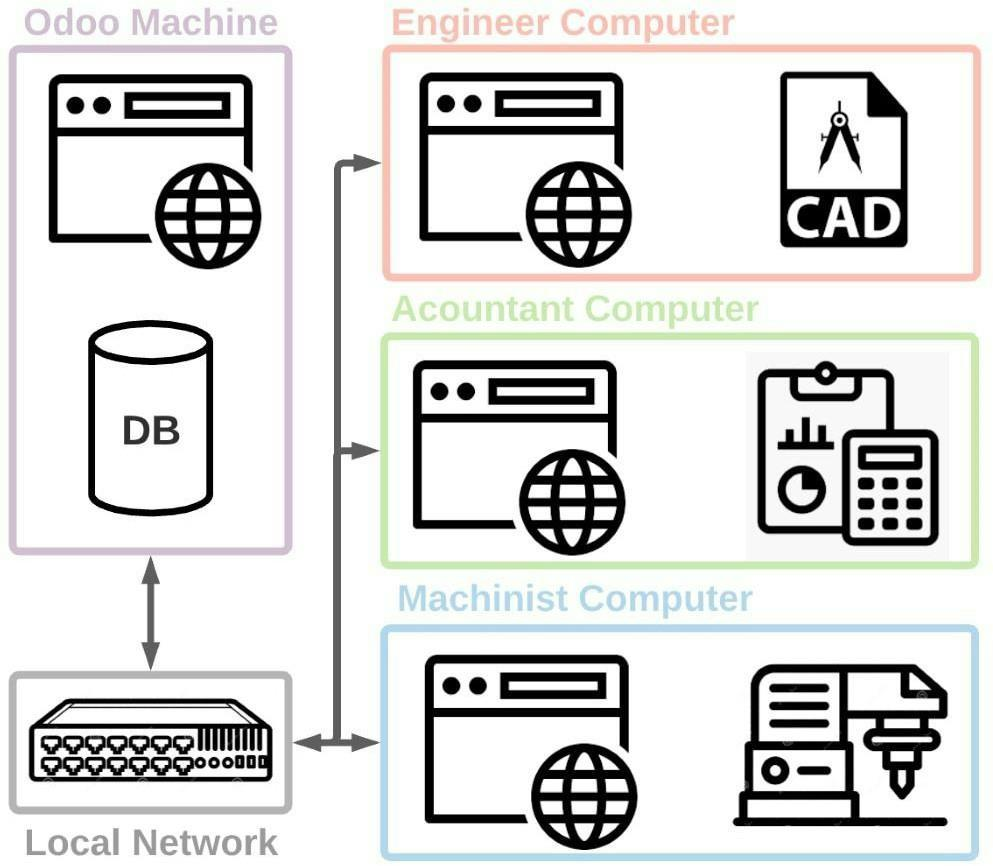
\includegraphics[width=431.75pt,height=376.67pt]{latexImage_476b335cf2d167ded8094e6e433ea182.png}}
\put(105.38,-110.86){\fontsize{12.81913}{1}\usefont{T1}{ptm}{b}{n}\selectfont\color{color_29791}5.}
\put(114.9648,-110.86){\fontsize{12.81913}{1}\usefont{T1}{ptm}{b}{n}\selectfont\color{color_29791}1}
\put(121.4307,-110.86){\fontsize{12.81913}{1}\usefont{T1}{ptm}{b}{n}\selectfont\color{color_29791}.}
\put(124.5495,-110.86){\fontsize{12.81913}{1}\usefont{T1}{ptm}{b}{n}\selectfont\color{color_29791}1}
\put(131.0154,-110.86){\fontsize{12.81913}{1}\usefont{T1}{ptm}{b}{n}\selectfont\color{color_29791}.}
\put(134.3,-110.86){\fontsize{12.83539}{1}\usefont{T1}{ptm}{b}{n}\selectfont\color{color_29791} }
\put(137.66,-110.86){\fontsize{12.96}{1}\usefont{T1}{ptm}{b}{n}\selectfont\color{color_29791}工}
\put(150.3738,-110.86){\fontsize{12.96}{1}\usefont{T1}{ptm}{b}{n}\selectfont\color{color_29791}作}
\put(163.2171,-110.86){\fontsize{12.96}{1}\usefont{T1}{ptm}{b}{n}\selectfont\color{color_29791}原}
\put(176.0605,-110.86){\fontsize{12.96}{1}\usefont{T1}{ptm}{b}{n}\selectfont\color{color_29791}理}
\put(188.93,-110.86){\fontsize{12.96}{1}\usefont{T1}{ptm}{b}{n}\selectfont\color{color_29791} }
\put(63.024,-135.58){\fontsize{12.96}{1}\usefont{T1}{ptm}{b}{n}\selectfont\color{color_29791} }
\put(82.944,-153.58){\fontsize{12}{1}\usefont{T1}{ptm}{m}{n}\selectfont\color{color_29791}該}
\put(95.292,-153.58){\fontsize{12}{1}\usefont{T1}{ptm}{m}{n}\selectfont\color{color_29791}軟}
\put(107.64,-153.58){\fontsize{12}{1}\usefont{T1}{ptm}{m}{n}\selectfont\color{color_29791}體}
\put(119.868,-153.58){\fontsize{12}{1}\usefont{T1}{ptm}{m}{n}\selectfont\color{color_29791}可}
\put(132.216,-153.58){\fontsize{12}{1}\usefont{T1}{ptm}{m}{n}\selectfont\color{color_29791}以}
\put(144.444,-153.58){\fontsize{12}{1}\usefont{T1}{ptm}{m}{n}\selectfont\color{color_29791}安}
\put(156.792,-153.58){\fontsize{12}{1}\usefont{T1}{ptm}{m}{n}\selectfont\color{color_29791}裝}
\put(169.02,-153.58){\fontsize{12}{1}\usefont{T1}{ptm}{m}{n}\selectfont\color{color_29791}在}
\put(181.368,-153.58){\fontsize{12}{1}\usefont{T1}{ptm}{m}{n}\selectfont\color{color_29791}大}
\put(193.596,-153.58){\fontsize{12}{1}\usefont{T1}{ptm}{m}{n}\selectfont\color{color_29791}多}
\put(205.944,-153.58){\fontsize{12}{1}\usefont{T1}{ptm}{m}{n}\selectfont\color{color_29791}數}
\put(218.45,-153.58){\fontsize{12}{1}\usefont{T1}{ptm}{m}{n}\selectfont\color{color_29791} }
\put(224.81,-153.58){\fontsize{12}{1}\usefont{T1}{ptm}{m}{n}\selectfont\color{color_29791}x86}
\put(242.81,-153.58){\fontsize{12}{1}\usefont{T1}{ptm}{m}{n}\selectfont\color{color_29791}  }
\put(252.65,-153.58){\fontsize{12}{1}\usefont{T1}{ptm}{m}{n}\selectfont\color{color_29791}計}
\put(264.758,-153.58){\fontsize{12}{1}\usefont{T1}{ptm}{m}{n}\selectfont\color{color_29791}算}
\put(276.986,-153.58){\fontsize{12}{1}\usefont{T1}{ptm}{m}{n}\selectfont\color{color_29791}機}
\put(289.214,-153.58){\fontsize{12}{1}\usefont{T1}{ptm}{m}{n}\selectfont\color{color_29791}中}
\put(301.322,-153.58){\fontsize{12}{1}\usefont{T1}{ptm}{m}{n}\selectfont\color{color_29791},}
\put(313.43,-153.58){\fontsize{12}{1}\usefont{T1}{ptm}{m}{n}\selectfont\color{color_29791}它}
\put(325.658,-153.58){\fontsize{12}{1}\usefont{T1}{ptm}{m}{n}\selectfont\color{color_29791}支}
\put(337.886,-153.58){\fontsize{12}{1}\usefont{T1}{ptm}{m}{n}\selectfont\color{color_29791}援}
\put(350.114,-153.58){\fontsize{12}{1}\usefont{T1}{ptm}{m}{n}\selectfont\color{color_29791}多}
\put(362.222,-153.58){\fontsize{12}{1}\usefont{T1}{ptm}{m}{n}\selectfont\color{color_29791}種}
\put(374.45,-153.58){\fontsize{12}{1}\usefont{T1}{ptm}{m}{n}\selectfont\color{color_29791}操}
\put(386.678,-153.58){\fontsize{12}{1}\usefont{T1}{ptm}{m}{n}\selectfont\color{color_29791}作}
\put(398.786,-153.58){\fontsize{12}{1}\usefont{T1}{ptm}{m}{n}\selectfont\color{color_29791}系}
\put(411.014,-153.58){\fontsize{12}{1}\usefont{T1}{ptm}{m}{n}\selectfont\color{color_29791}統}
\put(423.242,-153.58){\fontsize{12}{1}\usefont{T1}{ptm}{m}{n}\selectfont\color{color_29791},}
\put(435.35,-153.58){\fontsize{12}{1}\usefont{T1}{ptm}{m}{n}\selectfont\color{color_29791}包}
\put(447.578,-153.58){\fontsize{12}{1}\usefont{T1}{ptm}{m}{n}\selectfont\color{color_29791}括}
\put(460.06,-153.58){\fontsize{12}{1}\usefont{T1}{ptm}{m}{n}\selectfont\color{color_29791} }
\put(466.3,-153.58){\fontsize{12}{1}\usefont{T1}{ptm}{m}{n}\selectfont\color{color_29791}W}
\put(477.46,-153.58){\fontsize{12}{1}\usefont{T1}{ptm}{m}{n}\selectfont\color{color_29791}i}
\put(480.7,-153.58){\fontsize{12}{1}\usefont{T1}{ptm}{m}{n}\selectfont\color{color_29791}n}
\put(486.58,-153.58){\fontsize{12}{1}\usefont{T1}{ptm}{m}{n}\selectfont\color{color_29791}d}
\put(492.46,-153.58){\fontsize{12}{1}\usefont{T1}{ptm}{m}{n}\selectfont\color{color_29791}o}
\put(498.34,-153.58){\fontsize{12}{1}\usefont{T1}{ptm}{m}{n}\selectfont\color{color_29791}w}
\put(506.86,-153.58){\fontsize{12}{1}\usefont{T1}{ptm}{m}{n}\selectfont\color{color_29791}s}
\put(511.54,-153.58){\fontsize{12}{1}\usefont{T1}{ptm}{m}{n}\selectfont\color{color_29791} }
\put(69.384,-171.58){\fontsize{12}{1}\usefont{T1}{ptm}{m}{n}\selectfont\color{color_29791}和}
\put(80.90401,-171.58){\fontsize{12}{1}\usefont{T1}{ptm}{m}{n}\selectfont\color{color_29791}所}
\put(92.42401,-171.58){\fontsize{12}{1}\usefont{T1}{ptm}{m}{n}\selectfont\color{color_29791}有}
\put(103.944,-171.58){\fontsize{12}{1}\usefont{T1}{ptm}{m}{n}\selectfont\color{color_29791}主}
\put(115.464,-171.58){\fontsize{12}{1}\usefont{T1}{ptm}{m}{n}\selectfont\color{color_29791}要}
\put(127.104,-171.58){\fontsize{12}{1}\usefont{T1}{ptm}{m}{n}\selectfont\color{color_29791}的}
\put(138.62,-171.58){\fontsize{12}{1}\usefont{T1}{ptm}{m}{n}\selectfont\color{color_29791} }
\put(144.14,-171.58){\fontsize{12}{1}\usefont{T1}{ptm}{m}{n}\selectfont\color{color_29791}Linux}
\put(172.82,-171.58){\fontsize{12}{1}\usefont{T1}{ptm}{m}{n}\selectfont\color{color_29791} }
\put(175.7,-171.58){\fontsize{12}{1}\usefont{T1}{ptm}{m}{n}\selectfont\color{color_29791}發行版。}
\put(223.13,-171.58){\fontsize{12}{1}\usefont{T1}{ptm}{m}{n}\selectfont\color{color_29791} }
\put(63.024,-189.82){\fontsize{12}{1}\usefont{T1}{ptm}{m}{n}\selectfont\color{color_29791} }
\put(82.944,-205.42){\fontsize{12}{1}\usefont{T1}{ptm}{m}{n}\selectfont\color{color_29791}理想情況下,}
\put(154.22,-205.42){\fontsize{12}{1}\usefont{T1}{ptm}{m}{n}\selectfont\color{color_29791}Od}
\put(168.74,-205.42){\fontsize{12}{1}\usefont{T1}{ptm}{m}{n}\selectfont\color{color_29791}o}
\put(174.62,-205.42){\fontsize{12}{1}\usefont{T1}{ptm}{m}{n}\selectfont\color{color_29791}o}
\put(180.65,-205.42){\fontsize{12}{1}\usefont{T1}{ptm}{m}{n}\selectfont\color{color_29791} }
\put(203.93,-205.42){\fontsize{12}{1}\usefont{T1}{ptm}{m}{n}\selectfont\color{color_29791}軟體安裝在連接到局域網的計算機中,並啟動一}
\put(455.98,-205.42){\fontsize{12}{1}\usefont{T1}{ptm}{m}{n}\selectfont\color{color_29791}個}
\put(467.5,-205.42){\fontsize{12}{1}\usefont{T1}{ptm}{m}{n}\selectfont\color{color_29791} }
\put(490.3,-205.42){\fontsize{12}{1}\usefont{T1}{ptm}{m}{n}\selectfont\color{color_29791}S}
\put(496.78,-205.42){\fontsize{12}{1}\usefont{T1}{ptm}{m}{n}\selectfont\color{color_29791}Q}
\put(505.18,-205.42){\fontsize{12}{1}\usefont{T1}{ptm}{m}{n}\selectfont\color{color_29791}L}
\put(512.26,-205.42){\fontsize{12}{1}\usefont{T1}{ptm}{m}{n}\selectfont\color{color_29791} }
\put(69.384,-223.18){\fontsize{12}{1}\usefont{T1}{ptm}{m}{n}\selectfont\color{color_29791}資料庫,該資料庫包含企業生成的所有必要資訊和檔(}
\put(357.43,-223.18){\fontsize{12}{1}\usefont{T1}{ptm}{m}{n}\selectfont\color{color_29791}圖}
\put(368.95,-223.18){\fontsize{12}{1}\usefont{T1}{ptm}{m}{n}\selectfont\color{color_29791} }
\put(69.384,-241.06){\fontsize{12}{1}\usefont{T1}{ptm}{m}{n}\selectfont\color{color_29791}16}
\put(81.264,-241.06){\fontsize{12}{1}\usefont{T1}{ptm}{m}{n}\selectfont\color{color_29791})。所述計算機基本}
\put(189.372,-241.06){\fontsize{12}{1}\usefont{T1}{ptm}{m}{n}\selectfont\color{color_29791}上作為伺服器工作,並}
\put(309.48,-241.06){\fontsize{12}{1}\usefont{T1}{ptm}{m}{n}\selectfont\color{color_29791}由網路中存在的其他機}
\put(429.588,-241.06){\fontsize{12}{1}\usefont{T1}{ptm}{m}{n}\selectfont\color{color_29791}器通過瀏覽器}
\put(69.384,-258.97){\fontsize{12}{1}\usefont{T1}{ptm}{m}{n}\selectfont\color{color_29791}訪問。這台計算機可以}
\put(189.492,-258.97){\fontsize{12}{1}\usefont{T1}{ptm}{m}{n}\selectfont\color{color_29791}是專用伺服器,也可以}
\put(309.6,-258.97){\fontsize{12}{1}\usefont{T1}{ptm}{m}{n}\selectfont\color{color_29791}是正在使用的桌面,但}
\put(429.708,-258.97){\fontsize{12}{1}\usefont{T1}{ptm}{m}{n}\selectfont\color{color_29791}重要的是要記}
\put(69.384,-276.85){\fontsize{12}{1}\usefont{T1}{ptm}{m}{n}\selectfont\color{color_29791}住,它必須在軟體}
\put(164.532,-276.85){\fontsize{12}{1}\usefont{T1}{ptm}{m}{n}\selectfont\color{color_29791}運行}
\put(188.4,-276.85){\fontsize{12}{1}\usefont{T1}{ptm}{m}{n}\selectfont\color{color_29791}所需的整個過程中}
\put(283.548,-276.85){\fontsize{12}{1}\usefont{T1}{ptm}{m}{n}\selectfont\color{color_29791}保持}
\put(307.416,-276.85){\fontsize{12}{1}\usefont{T1}{ptm}{m}{n}\selectfont\color{color_29791}打開和連接。}
\put(378.91,-276.85){\fontsize{12}{1}\usefont{T1}{ptm}{m}{n}\selectfont\color{color_29791} }
\put(63.024,-287.29){\fontsize{4.56}{1}\usefont{T1}{ptm}{m}{n}\selectfont\color{color_29791} }
\put(153.74,-692.696){\fontsize{12}{1}\usefont{T1}{ptm}{b}{n}\selectfont\color{color_29791}圖}
\put(165.74,-692.696){\fontsize{12}{1}\usefont{T1}{ptm}{b}{n}\selectfont\color{color_29791}16}
\put(177.74,-692.696){\fontsize{12}{1}\usefont{T1}{ptm}{b}{n}\selectfont\color{color_29791} }
\put(180.53,-692.696){\fontsize{12}{1}\usefont{T1}{ptm}{b}{n}\selectfont\color{color_29791}Od}
\put(196.598,-692.696){\fontsize{12}{1}\usefont{T1}{ptm}{b}{n}\selectfont\color{color_29791}oo}
\put(208.61,-692.696){\fontsize{12}{1}\usefont{T1}{ptm}{b}{n}\selectfont\color{color_29791}配置}
\put(232.61,-692.696){\fontsize{12}{1}\usefont{T1}{ptm}{b}{n}\selectfont\color{color_29791}A}
\put(241.25,-692.696){\fontsize{12}{1}\usefont{T1}{ptm}{b}{n}\selectfont\color{color_29791}功}
\put(253.01,-692.696){\fontsize{12}{1}\usefont{T1}{ptm}{b}{n}\selectfont\color{color_29791}能}
\put(264.89,-692.696){\fontsize{12}{1}\usefont{T1}{ptm}{b}{n}\selectfont\color{color_29791}圖}
\put(276.65,-692.696){\fontsize{12}{1}\usefont{T1}{ptm}{b}{n}\selectfont\color{color_29791} }
\end{picture}
\newpage
\begin{tikzpicture}[overlay]\path(0pt,0pt);\end{tikzpicture}
\begin{picture}(-5,0)(2.5,0)
\put(500.26,-727.616){\fontsize{12}{1}\usefont{T1}{ptm}{m}{n}\selectfont\color{color_29791}25}
\put(511.78,-727.616){\fontsize{12}{1}\usefont{T1}{ptm}{m}{n}\selectfont\color{color_29791} }
\put(63.024,-726.896){\fontsize{9.96}{1}\usefont{T1}{ptm}{m}{n}\selectfont\color{color_29791} }
\put(80.65,-443.94){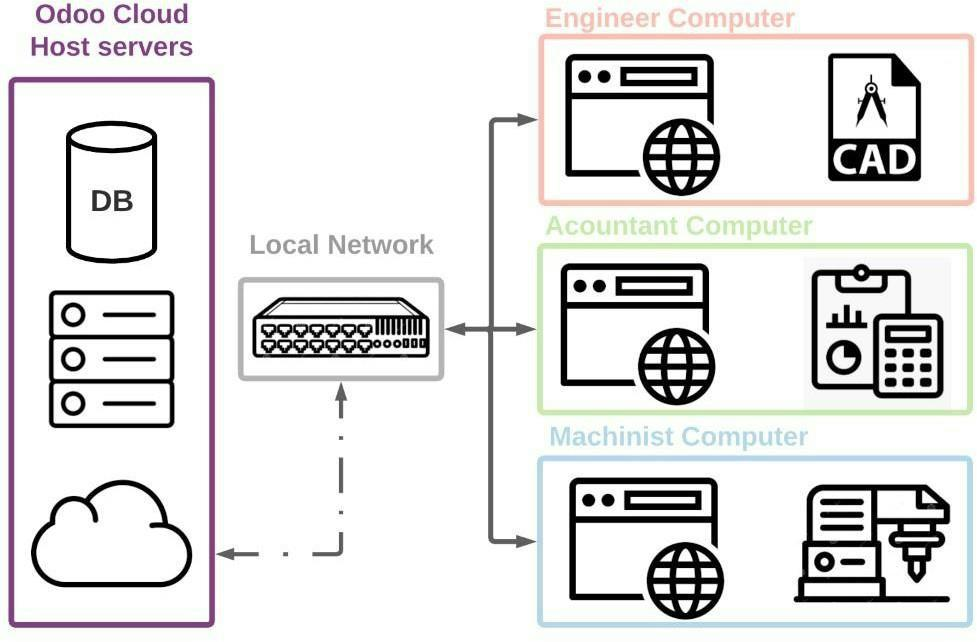
\includegraphics[width=417.7pt,height=274.44pt]{latexImage_fd4e4d2c76b3eb4b34df52bb1db4324b.png}}
\put(82.944,-88.29999){\fontsize{12}{1}\usefont{T1}{ptm}{m}{n}\selectfont\color{color_29791}另一種選擇是使用}
\put(178.94,-88.29999){\fontsize{12}{1}\usefont{T1}{ptm}{m}{n}\selectfont\color{color_29791} }
\put(240.29,-88.29999){\fontsize{12}{1}\usefont{T1}{ptm}{m}{n}\selectfont\color{color_29791}Odoo}
\put(266.93,-88.29999){\fontsize{12}{1}\usefont{T1}{ptm}{m}{n}\selectfont\color{color_29791} }
\put(328.39,-88.29999){\fontsize{12}{1}\usefont{T1}{ptm}{m}{n}\selectfont\color{color_29791}SA}
\put(343.75,-88.29999){\fontsize{12}{1}\usefont{T1}{ptm}{m}{n}\selectfont\color{color_29791} }
\put(404.47,-88.29999){\fontsize{12}{1}\usefont{T1}{ptm}{m}{n}\selectfont\color{color_29791}提供的託管服務(}
\put(500.5,-88.29999){\fontsize{12}{1}\usefont{T1}{ptm}{m}{n}\selectfont\color{color_29791}圖}
\put(511.54,-88.29999){\fontsize{12}{1}\usefont{T1}{ptm}{m}{n}\selectfont\color{color_29791} }
\put(69.384,-106.06){\fontsize{12}{1}\usefont{T1}{ptm}{m}{n}\selectfont\color{color_29791}17}
\put(81.384,-106.06){\fontsize{12}{1}\usefont{T1}{ptm}{m}{n}\selectfont\color{color_29791})}
\put(93.38,-106.06){\fontsize{12}{1}\usefont{T1}{ptm}{m}{n}\selectfont\color{color_29791}。}
\put(105.38,-106.06){\fontsize{12}{1}\usefont{T1}{ptm}{m}{n}\selectfont\color{color_29791}在這種情況下,系統將由他們託管,數據將存儲在他們的雲中。這非常適合}
\put(69.384,-123.94){\fontsize{12}{1}\usefont{T1}{ptm}{m}{n}\selectfont\color{color_29791}許多小型企}
\put(129.38,-123.94){\fontsize{12}{1}\usefont{T1}{ptm}{m}{n}\selectfont\color{color_29791}業}
\put(141.38,-123.94){\fontsize{12}{1}\usefont{T1}{ptm}{m}{n}\selectfont\color{color_29791},特別是如果他們特別喜歡與網站相關的模}
\put(369.43,-123.94){\fontsize{12}{1}\usefont{T1}{ptm}{m}{n}\selectfont\color{color_29791}組}
\put(381.43,-123.94){\fontsize{12}{1}\usefont{T1}{ptm}{m}{n}\selectfont\color{color_29791}(用於構建和管理網站}
\put(69.384,-141.94){\fontsize{12}{1}\usefont{T1}{ptm}{m}{n}\selectfont\color{color_29791}和電子商}
\put(117.38,-141.94){\fontsize{12}{1}\usefont{T1}{ptm}{m}{n}\selectfont\color{color_29791}店}
\put(129.38,-141.94){\fontsize{12}{1}\usefont{T1}{ptm}{m}{n}\selectfont\color{color_29791})。但是,它依賴於網路,在某些情況下可能會帶來問題。}
\put(441.46,-141.94){\fontsize{12}{1}\usefont{T1}{ptm}{m}{n}\selectfont\color{color_29791} }
\put(63.024,-165.58){\fontsize{9.96}{1}\usefont{T1}{ptm}{m}{n}\selectfont\color{color_29791} }
\put(229.85,-459.75){\fontsize{12}{1}\usefont{T1}{ptm}{b}{n}\selectfont\color{color_29791}圖}
\put(241.85,-459.75){\fontsize{12}{1}\usefont{T1}{ptm}{b}{n}\selectfont\color{color_29791}17}
\put(253.85,-459.75){\fontsize{12}{1}\usefont{T1}{ptm}{b}{n}\selectfont\color{color_29791} }
\put(256.73,-459.75){\fontsize{12}{1}\usefont{T1}{ptm}{b}{n}\selectfont\color{color_29791}Od}
\put(272.798,-459.75){\fontsize{12}{1}\usefont{T1}{ptm}{b}{n}\selectfont\color{color_29791}oo}
\put(284.81,-459.75){\fontsize{12}{1}\usefont{T1}{ptm}{b}{n}\selectfont\color{color_29791}配置}
\put(308.81,-459.75){\fontsize{12}{1}\usefont{T1}{ptm}{b}{n}\selectfont\color{color_29791}B}
\put(316.87,-459.75){\fontsize{12}{1}\usefont{T1}{ptm}{b}{n}\selectfont\color{color_29791}功能圖}
\put(352.15,-459.75){\fontsize{12}{1}\usefont{T1}{ptm}{b}{n}\selectfont\color{color_29791} }
\put(82.944,-492.63){\fontsize{12}{1}\usefont{T1}{ptm}{m}{n}\selectfont\color{color_29791}使用者基本上通過}
\put(178.092,-492.63){\fontsize{12}{1}\usefont{T1}{ptm}{m}{n}\selectfont\color{color_29791}圖形}
\put(201.96,-492.63){\fontsize{12}{1}\usefont{T1}{ptm}{m}{n}\selectfont\color{color_29791}使用者介面}
\put(261.53,-492.63){\fontsize{12}{1}\usefont{T1}{ptm}{m}{n}\selectfont\color{color_29791} }
\put(467.26,-492.63){\fontsize{12}{1}\usefont{T1}{ptm}{m}{n}\selectfont\color{color_29791}(}
\put(479.14,-492.63){\fontsize{12}{1}\usefont{T1}{ptm}{m}{n}\selectfont\color{color_29791}G}
\put(487.66,-492.63){\fontsize{12}{1}\usefont{T1}{ptm}{m}{n}\selectfont\color{color_29791}UI}
\put(500.14,-492.63){\fontsize{12}{1}\usefont{T1}{ptm}{m}{n}\selectfont\color{color_29791})}
\put(69.384,-510.39){\fontsize{12}{1}\usefont{T1}{ptm}{m}{n}\selectfont\color{color_29791}與系統交互,並使}
\put(164.532,-510.39){\fontsize{12}{1}\usefont{T1}{ptm}{m}{n}\selectfont\color{color_29791}用它}
\put(188.4,-510.39){\fontsize{12}{1}\usefont{T1}{ptm}{m}{n}\selectfont\color{color_29791}來訪問每個用戶根}
\put(283.548,-510.39){\fontsize{12}{1}\usefont{T1}{ptm}{m}{n}\selectfont\color{color_29791}據需}
\put(307.416,-510.39){\fontsize{12}{1}\usefont{T1}{ptm}{m}{n}\selectfont\color{color_29791}要提供的不同模組}
\put(402.564,-510.39){\fontsize{12}{1}\usefont{T1}{ptm}{m}{n}\selectfont\color{color_29791}。}
\put(414.67,-510.39){\fontsize{12}{1}\usefont{T1}{ptm}{m}{n}\selectfont\color{color_29791} }
\put(69.384,-528.15){\fontsize{12}{1}\usefont{T1}{ptm}{m}{n}\selectfont\color{color_29791}這意味}
\put(105.264,-528.15){\fontsize{12}{1}\usefont{T1}{ptm}{m}{n}\selectfont\color{color_29791}著可以}
\put(141.144,-528.15){\fontsize{12}{1}\usefont{T1}{ptm}{m}{n}\selectfont\color{color_29791}對不}
\put(165.024,-528.15){\fontsize{12}{1}\usefont{T1}{ptm}{m}{n}\selectfont\color{color_29791}同的}
\put(188.904,-528.15){\fontsize{12}{1}\usefont{T1}{ptm}{m}{n}\selectfont\color{color_29791}使用者}
\put(224.784,-528.15){\fontsize{12}{1}\usefont{T1}{ptm}{m}{n}\selectfont\color{color_29791}施加限}
\put(260.664,-528.15){\fontsize{12}{1}\usefont{T1}{ptm}{m}{n}\selectfont\color{color_29791}制,}
\put(284.544,-528.15){\fontsize{12}{1}\usefont{T1}{ptm}{m}{n}\selectfont\color{color_29791}以保}
\put(308.424,-528.15){\fontsize{12}{1}\usefont{T1}{ptm}{m}{n}\selectfont\color{color_29791}持對商}
\put(344.304,-528.15){\fontsize{12}{1}\usefont{T1}{ptm}{m}{n}\selectfont\color{color_29791}務活動}
\put(380.1841,-528.15){\fontsize{12}{1}\usefont{T1}{ptm}{m}{n}\selectfont\color{color_29791}不同}
\put(404.0641,-528.15){\fontsize{12}{1}\usefont{T1}{ptm}{m}{n}\selectfont\color{color_29791}方面}
\put(427.9441,-528.15){\fontsize{12}{1}\usefont{T1}{ptm}{m}{n}\selectfont\color{color_29791}的控制}
\put(463.8241,-528.15){\fontsize{12}{1}\usefont{T1}{ptm}{m}{n}\selectfont\color{color_29791},例如}
\put(499.78,-528.15){\fontsize{12}{1}\usefont{T1}{ptm}{m}{n}\selectfont\color{color_29791} }
\put(69.384,-545.91){\fontsize{12}{1}\usefont{T1}{ptm}{m}{n}\selectfont\color{color_29791},會計}
\put(105.264,-545.91){\fontsize{12}{1}\usefont{T1}{ptm}{m}{n}\selectfont\color{color_29791}師可以}
\put(141.144,-545.91){\fontsize{12}{1}\usefont{T1}{ptm}{m}{n}\selectfont\color{color_29791}訪問}
\put(165.024,-545.91){\fontsize{12}{1}\usefont{T1}{ptm}{m}{n}\selectfont\color{color_29791}會計}
\put(188.904,-545.91){\fontsize{12}{1}\usefont{T1}{ptm}{m}{n}\selectfont\color{color_29791}模組、}
\put(224.784,-545.91){\fontsize{12}{1}\usefont{T1}{ptm}{m}{n}\selectfont\color{color_29791}銷售模}
\put(260.664,-545.91){\fontsize{12}{1}\usefont{T1}{ptm}{m}{n}\selectfont\color{color_29791}組和}
\put(284.544,-545.91){\fontsize{12}{1}\usefont{T1}{ptm}{m}{n}\selectfont\color{color_29791}庫存}
\put(308.424,-545.91){\fontsize{12}{1}\usefont{T1}{ptm}{m}{n}\selectfont\color{color_29791}模組,}
\put(344.304,-545.91){\fontsize{12}{1}\usefont{T1}{ptm}{m}{n}\selectfont\color{color_29791}但他們}
\put(380.1841,-545.91){\fontsize{12}{1}\usefont{T1}{ptm}{m}{n}\selectfont\color{color_29791}將受}
\put(404.0641,-545.91){\fontsize{12}{1}\usefont{T1}{ptm}{m}{n}\selectfont\color{color_29791}到製}
\put(427.9441,-545.91){\fontsize{12}{1}\usefont{T1}{ptm}{m}{n}\selectfont\color{color_29791}造模組}
\put(463.8241,-545.91){\fontsize{12}{1}\usefont{T1}{ptm}{m}{n}\selectfont\color{color_29791}的限制}
\put(499.78,-545.91){\fontsize{12}{1}\usefont{T1}{ptm}{m}{n}\selectfont\color{color_29791} }
\put(69.384,-563.91){\fontsize{12}{1}\usefont{T1}{ptm}{m}{n}\selectfont\color{color_29791}。這種}
\put(105.264,-563.91){\fontsize{12}{1}\usefont{T1}{ptm}{m}{n}\selectfont\color{color_29791}限制保}
\put(141.144,-563.91){\fontsize{12}{1}\usefont{T1}{ptm}{m}{n}\selectfont\color{color_29791}證了}
\put(165.024,-563.91){\fontsize{12}{1}\usefont{T1}{ptm}{m}{n}\selectfont\color{color_29791}對流}
\put(188.904,-563.91){\fontsize{12}{1}\usefont{T1}{ptm}{m}{n}\selectfont\color{color_29791}程的控}
\put(224.784,-563.91){\fontsize{12}{1}\usefont{T1}{ptm}{m}{n}\selectfont\color{color_29791}制只對}
\put(260.664,-563.91){\fontsize{12}{1}\usefont{T1}{ptm}{m}{n}\selectfont\color{color_29791}適當}
\put(284.544,-563.91){\fontsize{12}{1}\usefont{T1}{ptm}{m}{n}\selectfont\color{color_29791}的員}
\put(308.424,-563.91){\fontsize{12}{1}\usefont{T1}{ptm}{m}{n}\selectfont\color{color_29791}工。}
\put(332.35,-563.91){\fontsize{12}{1}\usefont{T1}{ptm}{m}{n}\selectfont\color{color_29791} }
\put(63.024,-581.46){\fontsize{12}{1}\usefont{T1}{ptm}{m}{n}\selectfont\color{color_29791} }
\put(82.944,-597.06){\fontsize{12}{1}\usefont{T1}{ptm}{m}{n}\selectfont\color{color_29791}在上述}
\put(118.94,-597.06){\fontsize{12}{1}\usefont{T1}{ptm}{m}{n}\selectfont\color{color_29791} }
\put(197.09,-597.06){\fontsize{12}{1}\usefont{T1}{ptm}{m}{n}\selectfont\color{color_29791}G}
\put(205.73,-597.06){\fontsize{12}{1}\usefont{T1}{ptm}{m}{n}\selectfont\color{color_29791}U}
\put(214.49,-597.06){\fontsize{12}{1}\usefont{T1}{ptm}{m}{n}\selectfont\color{color_29791}I}
\put(218.45,-597.06){\fontsize{12}{1}\usefont{T1}{ptm}{m}{n}\selectfont\color{color_29791} }
\put(296.33,-597.06){\fontsize{12}{1}\usefont{T1}{ptm}{m}{n}\selectfont\color{color_29791}中}
\put(308.33,-597.06){\fontsize{12}{1}\usefont{T1}{ptm}{m}{n}\selectfont\color{color_29791},}
\put(320.47,-597.06){\fontsize{12}{1}\usefont{T1}{ptm}{m}{n}\selectfont\color{color_29791}不同的模組顯示為應用程式圖示(}
\put(500.5,-597.06){\fontsize{12}{1}\usefont{T1}{ptm}{m}{n}\selectfont\color{color_29791}圖}
\put(511.66,-597.06){\fontsize{12}{1}\usefont{T1}{ptm}{m}{n}\selectfont\color{color_29791} }
\put(69.384,-614.94){\fontsize{12}{1}\usefont{T1}{ptm}{m}{n}\selectfont\color{color_29791}18}
\put(81.384,-614.94){\fontsize{12}{1}\usefont{T1}{ptm}{m}{n}\selectfont\color{color_29791})}
\put(93.38,-614.94){\fontsize{12}{1}\usefont{T1}{ptm}{m}{n}\selectfont\color{color_29791},}
\put(105.38,-614.94){\fontsize{12}{1}\usefont{T1}{ptm}{m}{n}\selectfont\color{color_29791}從一開始,該公司就提供了合理選擇的集成良好的應用程}
\put(405.43,-614.94){\fontsize{12}{1}\usefont{T1}{ptm}{m}{n}\selectfont\color{color_29791}式}
\put(417.43,-614.94){\fontsize{12}{1}\usefont{T1}{ptm}{m}{n}\selectfont\color{color_29791},更不用說充滿}
\put(69.384,-632.82){\fontsize{12}{1}\usefont{T1}{ptm}{m}{n}\selectfont\color{color_29791}社區製作模組的龐大應用程式商店了。}
\put(273.41,-632.82){\fontsize{12}{1}\usefont{T1}{ptm}{m}{n}\selectfont\color{color_29791} }
\end{picture}
\newpage
\begin{tikzpicture}[overlay]\path(0pt,0pt);\end{tikzpicture}
\begin{picture}(-5,0)(2.5,0)
\put(500.26,-727.616){\fontsize{12}{1}\usefont{T1}{ptm}{m}{n}\selectfont\color{color_29791}26}
\put(511.78,-727.616){\fontsize{12}{1}\usefont{T1}{ptm}{m}{n}\selectfont\color{color_29791} }
\put(63.024,-726.896){\fontsize{9.96}{1}\usefont{T1}{ptm}{m}{n}\selectfont\color{color_29791} }
\put(519.22,-217.18){\fontsize{9.96}{1}\usefont{T1}{ptm}{m}{n}\selectfont\color{color_29791} }
\put(190.13,-238.06){\fontsize{12}{1}\usefont{T1}{ptm}{b}{n}\selectfont\color{color_29791}圖}
\put(202.13,-238.06){\fontsize{12}{1}\usefont{T1}{ptm}{b}{n}\selectfont\color{color_29791} }
\put(205.13,-238.06){\fontsize{12}{1}\usefont{T1}{ptm}{b}{n}\selectfont\color{color_29791}18}
\put(217.13,-238.06){\fontsize{12}{1}\usefont{T1}{ptm}{b}{n}\selectfont\color{color_29791} }
\put(220.01,-238.06){\fontsize{12}{1}\usefont{T1}{ptm}{b}{n}\selectfont\color{color_29791}配置}
\put(244.01,-238.06){\fontsize{12}{1}\usefont{T1}{ptm}{b}{n}\selectfont\color{color_29791} }
\put(247.01,-238.06){\fontsize{12}{1}\usefont{T1}{ptm}{b}{n}\selectfont\color{color_29791}B}
\put(255.05,-238.06){\fontsize{12}{1}\usefont{T1}{ptm}{b}{n}\selectfont\color{color_29791} }
\put(257.93,-238.06){\fontsize{12}{1}\usefont{T1}{ptm}{b}{n}\selectfont\color{color_29791}中}
\put(269.93,-238.06){\fontsize{12}{1}\usefont{T1}{ptm}{b}{n}\selectfont\color{color_29791} }
\put(272.93,-238.06){\fontsize{12}{1}\usefont{T1}{ptm}{b}{n}\selectfont\color{color_29791}Od}
\put(288.998,-238.06){\fontsize{12}{1}\usefont{T1}{ptm}{b}{n}\selectfont\color{color_29791}oo}
\put(301.01,-238.06){\fontsize{12}{1}\usefont{T1}{ptm}{b}{n}\selectfont\color{color_29791} }
\put(303.77,-238.06){\fontsize{12}{1}\usefont{T1}{ptm}{b}{n}\selectfont\color{color_29791}的}
\put(315.79,-238.06){\fontsize{12}{1}\usefont{T1}{ptm}{b}{n}\selectfont\color{color_29791} }
\put(318.79,-238.06){\fontsize{12}{1}\usefont{T1}{ptm}{b}{n}\selectfont\color{color_29791}GUI}
\put(341.47,-238.06){\fontsize{12}{1}\usefont{T1}{ptm}{b}{n}\selectfont\color{color_29791} }
\put(344.47,-238.06){\fontsize{12}{1}\usefont{T1}{ptm}{b}{n}\selectfont\color{color_29791}螢幕截圖}
\put(391.87,-238.06){\fontsize{12}{1}\usefont{T1}{ptm}{b}{n}\selectfont\color{color_29791} }
\put(106.1,-276.01){\fontsize{12.81913}{1}\usefont{T1}{ptm}{b}{n}\selectfont\color{color_29791}5.}
\put(115.6848,-276.01){\fontsize{12.81913}{1}\usefont{T1}{ptm}{b}{n}\selectfont\color{color_29791}1}
\put(122.1507,-276.01){\fontsize{12.81913}{1}\usefont{T1}{ptm}{b}{n}\selectfont\color{color_29791}.}
\put(125.2695,-276.01){\fontsize{12.81913}{1}\usefont{T1}{ptm}{b}{n}\selectfont\color{color_29791}2}
\put(131.7354,-276.01){\fontsize{12.81913}{1}\usefont{T1}{ptm}{b}{n}\selectfont\color{color_29791}.}
\put(135.02,-276.01){\fontsize{12.83539}{1}\usefont{T1}{ptm}{b}{n}\selectfont\color{color_29791} }
\put(138.38,-276.01){\fontsize{12.96}{1}\usefont{T1}{ptm}{b}{n}\selectfont\color{color_29791}O}
\put(148.3463,-276.01){\fontsize{12.96}{1}\usefont{T1}{ptm}{b}{n}\selectfont\color{color_29791}d}
\put(155.4224,-276.01){\fontsize{12.96}{1}\usefont{T1}{ptm}{b}{n}\selectfont\color{color_29791}oo}
\put(168.26,-276.01){\fontsize{12.96}{1}\usefont{T1}{ptm}{b}{n}\selectfont\color{color_29791}對}
\put(181.1033,-276.01){\fontsize{12.96}{1}\usefont{T1}{ptm}{b}{n}\selectfont\color{color_29791}製}
\put(193.9467,-276.01){\fontsize{12.96}{1}\usefont{T1}{ptm}{b}{n}\selectfont\color{color_29791}造}
\put(206.6605,-276.01){\fontsize{12.96}{1}\usefont{T1}{ptm}{b}{n}\selectfont\color{color_29791}業}
\put(219.5038,-276.01){\fontsize{12.96}{1}\usefont{T1}{ptm}{b}{n}\selectfont\color{color_29791}的}
\put(232.3472,-276.01){\fontsize{12.96}{1}\usefont{T1}{ptm}{b}{n}\selectfont\color{color_29791}看}
\put(245.0609,-276.01){\fontsize{12.96}{1}\usefont{T1}{ptm}{b}{n}\selectfont\color{color_29791}法}
\put(257.9043,-276.01){\fontsize{12.96}{1}\usefont{T1}{ptm}{b}{n}\selectfont\color{color_29791}:}
\put(270.77,-276.01){\fontsize{12.96}{1}\usefont{T1}{ptm}{b}{n}\selectfont\color{color_29791} }
\put(82.944,-304.45){\fontsize{12}{1}\usefont{T1}{ptm}{m}{n}\selectfont\color{color_29791}O}
\put(91.464,-304.45){\fontsize{12}{1}\usefont{T1}{ptm}{m}{n}\selectfont\color{color_29791}d}
\put(97.344,-304.45){\fontsize{12}{1}\usefont{T1}{ptm}{m}{n}\selectfont\color{color_29791}o}
\put(103.224,-304.45){\fontsize{12}{1}\usefont{T1}{ptm}{m}{n}\selectfont\color{color_29791}o}
\put(109.34,-304.45){\fontsize{12}{1}\usefont{T1}{ptm}{m}{n}\selectfont\color{color_29791}認}
\put(121.448,-304.45){\fontsize{12}{1}\usefont{T1}{ptm}{m}{n}\selectfont\color{color_29791}為}
\put(133.556,-304.45){\fontsize{12}{1}\usefont{T1}{ptm}{m}{n}\selectfont\color{color_29791},}
\put(145.664,-304.45){\fontsize{12}{1}\usefont{T1}{ptm}{m}{n}\selectfont\color{color_29791}製}
\put(157.772,-304.45){\fontsize{12}{1}\usefont{T1}{ptm}{m}{n}\selectfont\color{color_29791}造}
\put(169.88,-304.45){\fontsize{12}{1}\usefont{T1}{ptm}{m}{n}\selectfont\color{color_29791}任}
\put(181.988,-304.45){\fontsize{12}{1}\usefont{T1}{ptm}{m}{n}\selectfont\color{color_29791}何產}
\put(206.096,-304.45){\fontsize{12}{1}\usefont{T1}{ptm}{m}{n}\selectfont\color{color_29791}品}
\put(218.204,-304.45){\fontsize{12}{1}\usefont{T1}{ptm}{m}{n}\selectfont\color{color_29791}的}
\put(230.312,-304.45){\fontsize{12}{1}\usefont{T1}{ptm}{m}{n}\selectfont\color{color_29791}責}
\put(242.42,-304.45){\fontsize{12}{1}\usefont{T1}{ptm}{m}{n}\selectfont\color{color_29791}任}
\put(254.528,-304.45){\fontsize{12}{1}\usefont{T1}{ptm}{m}{n}\selectfont\color{color_29791}都}
\put(266.636,-304.45){\fontsize{12}{1}\usefont{T1}{ptm}{m}{n}\selectfont\color{color_29791}分佈}
\put(290.744,-304.45){\fontsize{12}{1}\usefont{T1}{ptm}{m}{n}\selectfont\color{color_29791}在}
\put(302.852,-304.45){\fontsize{12}{1}\usefont{T1}{ptm}{m}{n}\selectfont\color{color_29791}不同}
\put(326.96,-304.45){\fontsize{12}{1}\usefont{T1}{ptm}{m}{n}\selectfont\color{color_29791}的}
\put(339.068,-304.45){\fontsize{12}{1}\usefont{T1}{ptm}{m}{n}\selectfont\color{color_29791}公}
\put(351.176,-304.45){\fontsize{12}{1}\usefont{T1}{ptm}{m}{n}\selectfont\color{color_29791}司}
\put(363.284,-304.45){\fontsize{12}{1}\usefont{T1}{ptm}{m}{n}\selectfont\color{color_29791}部}
\put(375.392,-304.45){\fontsize{12}{1}\usefont{T1}{ptm}{m}{n}\selectfont\color{color_29791}門}
\put(387.5,-304.45){\fontsize{12}{1}\usefont{T1}{ptm}{m}{n}\selectfont\color{color_29791},每}
\put(411.608,-304.45){\fontsize{12}{1}\usefont{T1}{ptm}{m}{n}\selectfont\color{color_29791}個}
\put(423.716,-304.45){\fontsize{12}{1}\usefont{T1}{ptm}{m}{n}\selectfont\color{color_29791}部門}
\put(447.824,-304.45){\fontsize{12}{1}\usefont{T1}{ptm}{m}{n}\selectfont\color{color_29791}負}
\put(459.932,-304.45){\fontsize{12}{1}\usefont{T1}{ptm}{m}{n}\selectfont\color{color_29791}責}
\put(472.04,-304.45){\fontsize{12}{1}\usefont{T1}{ptm}{m}{n}\selectfont\color{color_29791}特}
\put(484.148,-304.45){\fontsize{12}{1}\usefont{T1}{ptm}{m}{n}\selectfont\color{color_29791}定}
\put(496.256,-304.45){\fontsize{12}{1}\usefont{T1}{ptm}{m}{n}\selectfont\color{color_29791}的}
\put(69.384,-322.33){\fontsize{12}{1}\usefont{T1}{ptm}{m}{n}\selectfont\color{color_29791}檔類型,並使用特定的}
\put(189.492,-322.33){\fontsize{12}{1}\usefont{T1}{ptm}{m}{n}\selectfont\color{color_29791}應用程式進行處理(表}
\put(309.67,-322.33){\fontsize{12}{1}\usefont{T1}{ptm}{m}{n}\selectfont\color{color_29791}2}
\put(315.67,-322.33){\fontsize{12}{1}\usefont{T1}{ptm}{m}{n}\selectfont\color{color_29791})。從}
\put(351.67,-322.33){\fontsize{12}{1}\usefont{T1}{ptm}{m}{n}\selectfont\color{color_29791}P}
\put(358.27,-322.33){\fontsize{12}{1}\usefont{T1}{ptm}{m}{n}\selectfont\color{color_29791}L}
\put(365.47,-322.33){\fontsize{12}{1}\usefont{T1}{ptm}{m}{n}\selectfont\color{color_29791}M}
\put(376.15,-322.33){\fontsize{12}{1}\usefont{T1}{ptm}{m}{n}\selectfont\color{color_29791}的角度來}
\put(424.258,-322.33){\fontsize{12}{1}\usefont{T1}{ptm}{m}{n}\selectfont\color{color_29791}看,這是非常積}
\put(69.384,-340.21){\fontsize{12}{1}\usefont{T1}{ptm}{m}{n}\selectfont\color{color_29791}極的,因為正如(}
\put(166.34,-340.21){\fontsize{12}{1}\usefont{T1}{ptm}{m}{n}\selectfont\color{color_29791}S}
\put(172.94,-340.21){\fontsize{12}{1}\usefont{T1}{ptm}{m}{n}\selectfont\color{color_29791}a}
\put(178.22,-340.21){\fontsize{12}{1}\usefont{T1}{ptm}{m}{n}\selectfont\color{color_29791}a}
\put(183.38,-340.21){\fontsize{12}{1}\usefont{T1}{ptm}{m}{n}\selectfont\color{color_29791}ks}
\put(193.94,-340.21){\fontsize{12}{1}\usefont{T1}{ptm}{m}{n}\selectfont\color{color_29791}v}
\put(199.82,-340.21){\fontsize{12}{1}\usefont{T1}{ptm}{m}{n}\selectfont\color{color_29791}u}
\put(205.7,-340.21){\fontsize{12}{1}\usefont{T1}{ptm}{m}{n}\selectfont\color{color_29791}o}
\put(211.58,-340.21){\fontsize{12}{1}\usefont{T1}{ptm}{m}{n}\selectfont\color{color_29791}r}
\put(215.42,-340.21){\fontsize{12}{1}\usefont{T1}{ptm}{m}{n}\selectfont\color{color_29791}i}
\put(218.93,-340.21){\fontsize{12}{1}\usefont{T1}{ptm}{m}{n}\selectfont\color{color_29791}和}
\put(231.17,-340.21){\fontsize{12}{1}\usefont{T1}{ptm}{m}{n}\selectfont\color{color_29791}I}
\put(234.89,-340.21){\fontsize{12}{1}\usefont{T1}{ptm}{m}{n}\selectfont\color{color_29791}m}
\put(244.13,-340.21){\fontsize{12}{1}\usefont{T1}{ptm}{m}{n}\selectfont\color{color_29791}mo}
\put(259.37,-340.21){\fontsize{12}{1}\usefont{T1}{ptm}{m}{n}\selectfont\color{color_29791}n}
\put(265.25,-340.21){\fontsize{12}{1}\usefont{T1}{ptm}{m}{n}\selectfont\color{color_29791}e}
\put(270.41,-340.21){\fontsize{12}{1}\usefont{T1}{ptm}{m}{n}\selectfont\color{color_29791}n}
\put(276.53,-340.21){\fontsize{12}{1}\usefont{T1}{ptm}{m}{n}\selectfont\color{color_29791},}
\put(288.77,-340.21){\fontsize{12}{1}\usefont{T1}{ptm}{m}{n}\selectfont\color{color_29791}2}
\put(294.65,-340.21){\fontsize{12}{1}\usefont{T1}{ptm}{m}{n}\selectfont\color{color_29791}0}
\put(300.53,-340.21){\fontsize{12}{1}\usefont{T1}{ptm}{m}{n}\selectfont\color{color_29791}08}
\put(312.67,-340.21){\fontsize{12}{1}\usefont{T1}{ptm}{m}{n}\selectfont\color{color_29791})關於用戶許可權管}
\put(421.858,-340.21){\fontsize{12}{1}\usefont{T1}{ptm}{m}{n}\selectfont\color{color_29791}理所提到的,}
\put(494.62,-340.21){\fontsize{12}{1}\usefont{T1}{ptm}{m}{n}\selectfont\color{color_29791}P}
\put(501.22,-340.21){\fontsize{12}{1}\usefont{T1}{ptm}{m}{n}\selectfont\color{color_29791}L}
\put(508.42,-340.21){\fontsize{12}{1}\usefont{T1}{ptm}{m}{n}\selectfont\color{color_29791} }
\put(69.384,-358.09){\fontsize{12}{1}\usefont{T1}{ptm}{m}{n}\selectfont\color{color_29791}M}
\put(79.944,-358.09){\fontsize{12}{1}\usefont{T1}{ptm}{m}{n}\selectfont\color{color_29791}系統用於定義資訊}
\put(175.092,-358.09){\fontsize{12}{1}\usefont{T1}{ptm}{m}{n}\selectfont\color{color_29791}訪}
\put(187.08,-358.09){\fontsize{12}{1}\usefont{T1}{ptm}{m}{n}\selectfont\color{color_29791}問和維護許可權。}
\put(282.17,-358.09){\fontsize{12}{1}\usefont{T1}{ptm}{m}{n}\selectfont\color{color_29791}P}
\put(288.77,-358.09){\fontsize{12}{1}\usefont{T1}{ptm}{m}{n}\selectfont\color{color_29791}LM}
\put(306.77,-358.09){\fontsize{12}{1}\usefont{T1}{ptm}{m}{n}\selectfont\color{color_29791} }
\put(69.384,-376.09){\fontsize{12}{1}\usefont{T1}{ptm}{m}{n}\selectfont\color{color_29791}系統定義了可以創建新資訊或進行、檢查和接受更改的人員,以及僅允許查看系統}
\put(69.384,-393.97){\fontsize{12}{1}\usefont{T1}{ptm}{m}{n}\selectfont\color{color_29791}中的資訊或文檔的人員。在將}
\put(225.41,-393.97){\fontsize{12}{1}\usefont{T1}{ptm}{m}{n}\selectfont\color{color_29791} }
\put(487.9,-393.97){\fontsize{12}{1}\usefont{T1}{ptm}{m}{n}\selectfont\color{color_29791}P}
\put(494.5,-393.97){\fontsize{12}{1}\usefont{T1}{ptm}{m}{n}\selectfont\color{color_29791}L}
\put(501.22,-393.97){\fontsize{12}{1}\usefont{T1}{ptm}{m}{n}\selectfont\color{color_29791}M}
\put(511.54,-393.97){\fontsize{12}{1}\usefont{T1}{ptm}{m}{n}\selectfont\color{color_29791} }
\put(69.384,-411.87){\fontsize{12}{1}\usefont{T1}{ptm}{m}{n}\selectfont\color{color_29791}與}
\put(81.264,-411.87){\fontsize{12}{1}\usefont{T1}{ptm}{m}{n}\selectfont\color{color_29791}其}
\put(93.144,-411.87){\fontsize{12}{1}\usefont{T1}{ptm}{m}{n}\selectfont\color{color_29791}他}
\put(105.024,-411.87){\fontsize{12}{1}\usefont{T1}{ptm}{m}{n}\selectfont\color{color_29791}系}
\put(116.904,-411.87){\fontsize{12}{1}\usefont{T1}{ptm}{m}{n}\selectfont\color{color_29791}統}
\put(128.784,-411.87){\fontsize{12}{1}\usefont{T1}{ptm}{m}{n}\selectfont\color{color_29791}整}
\put(140.544,-411.87){\fontsize{12}{1}\usefont{T1}{ptm}{m}{n}\selectfont\color{color_29791}合}
\put(152.424,-411.87){\fontsize{12}{1}\usefont{T1}{ptm}{m}{n}\selectfont\color{color_29791}時}
\put(164.304,-411.87){\fontsize{12}{1}\usefont{T1}{ptm}{m}{n}\selectfont\color{color_29791},}
\put(176.184,-411.87){\fontsize{12}{1}\usefont{T1}{ptm}{m}{n}\selectfont\color{color_29791}用}
\put(187.944,-411.87){\fontsize{12}{1}\usefont{T1}{ptm}{m}{n}\selectfont\color{color_29791}戶}
\put(199.824,-411.87){\fontsize{12}{1}\usefont{T1}{ptm}{m}{n}\selectfont\color{color_29791}許}
\put(211.704,-411.87){\fontsize{12}{1}\usefont{T1}{ptm}{m}{n}\selectfont\color{color_29791}可}
\put(223.584,-411.87){\fontsize{12}{1}\usefont{T1}{ptm}{m}{n}\selectfont\color{color_29791}權}
\put(235.464,-411.87){\fontsize{12}{1}\usefont{T1}{ptm}{m}{n}\selectfont\color{color_29791}管}
\put(247.344,-411.87){\fontsize{12}{1}\usefont{T1}{ptm}{m}{n}\selectfont\color{color_29791}理}
\put(259.104,-411.87){\fontsize{12}{1}\usefont{T1}{ptm}{m}{n}\selectfont\color{color_29791}通}
\put(270.984,-411.87){\fontsize{12}{1}\usefont{T1}{ptm}{m}{n}\selectfont\color{color_29791}常}
\put(282.864,-411.87){\fontsize{12}{1}\usefont{T1}{ptm}{m}{n}\selectfont\color{color_29791}是}
\put(294.744,-411.87){\fontsize{12}{1}\usefont{T1}{ptm}{m}{n}\selectfont\color{color_29791}一}
\put(306.5041,-411.87){\fontsize{12}{1}\usefont{T1}{ptm}{m}{n}\selectfont\color{color_29791}個}
\put(318.3841,-411.87){\fontsize{12}{1}\usefont{T1}{ptm}{m}{n}\selectfont\color{color_29791}挑}
\put(330.2641,-411.87){\fontsize{12}{1}\usefont{T1}{ptm}{m}{n}\selectfont\color{color_29791}戰}
\put(342.1441,-411.87){\fontsize{12}{1}\usefont{T1}{ptm}{m}{n}\selectfont\color{color_29791}。}
\put(353.95,-411.87){\fontsize{12}{1}\usefont{T1}{ptm}{m}{n}\selectfont\color{color_29791} }
\put(202.73,-444.51){\fontsize{12}{1}\usefont{T1}{ptm}{b}{n}\selectfont\color{color_29791}表}
\put(214.73,-444.51){\fontsize{12}{1}\usefont{T1}{ptm}{b}{n}\selectfont\color{color_29791}2}
\put(220.73,-444.51){\fontsize{12}{1}\usefont{T1}{ptm}{b}{n}\selectfont\color{color_29791}部門與文檔}
\put(280.73,-444.51){\fontsize{12}{1}\usefont{T1}{ptm}{b}{n}\selectfont\color{color_29791}/}
\put(284.09,-444.51){\fontsize{12}{1}\usefont{T1}{ptm}{b}{n}\selectfont\color{color_29791}應用程式的相關性}
\put(379.27,-444.51){\fontsize{12}{1}\usefont{T1}{ptm}{b}{n}\selectfont\color{color_29791} }
\end{picture}
\begin{tikzpicture}[overlay]
\path(0pt,0pt);
\filldraw[color_254818][even odd rule]
(70.464pt, -474.87pt) -- (290.924pt, -474.87pt)
 -- (290.924pt, -474.87pt)
 -- (290.924pt, -449.91pt)
 -- (290.924pt, -449.91pt)
 -- (70.464pt, -449.91pt) -- cycle
;
\begin{scope}
\clip
(70.464pt, -474.87pt) -- (290.924pt, -474.87pt)
 -- (290.924pt, -474.87pt)
 -- (290.924pt, -449.91pt)
 -- (290.924pt, -449.91pt)
 -- (70.464pt, -449.91pt) -- cycle
;
\filldraw[color_254818][even odd rule]
(70.464pt, -473.91pt) -- (290.924pt, -473.91pt)
 -- (290.924pt, -473.91pt)
 -- (290.924pt, -449.91pt)
 -- (290.924pt, -449.91pt)
 -- (70.464pt, -449.91pt) -- cycle
;
\begin{scope}
\clip
(70.464pt, -474.87pt) -- (290.924pt, -474.87pt)
 -- (290.924pt, -474.87pt)
 -- (290.924pt, -449.91pt)
 -- (290.924pt, -449.91pt)
 -- (70.464pt, -449.91pt) -- cycle
;
\end{scope}
\end{scope}
\end{tikzpicture}
\begin{picture}(-5,0)(2.5,0)
\put(165.38,-469.11){\fontsize{15.96}{1}\usefont{T1}{ptm}{b}{n}\selectfont\color{color_29791}部門}
\put(196.85,-469.11){\fontsize{15.96}{1}\usefont{T1}{ptm}{b}{n}\selectfont\color{color_29791} }
\end{picture}
\begin{tikzpicture}[overlay]
\path(0pt,0pt);
\filldraw[color_214189][even odd rule]
(291.41pt, -474.87pt) -- (512.14pt, -474.87pt)
 -- (512.14pt, -474.87pt)
 -- (512.14pt, -449.91pt)
 -- (512.14pt, -449.91pt)
 -- (291.41pt, -449.91pt) -- cycle
;
\begin{scope}
\clip
(291.41pt, -474.87pt) -- (512.14pt, -474.87pt)
 -- (512.14pt, -474.87pt)
 -- (512.14pt, -449.91pt)
 -- (512.14pt, -449.91pt)
 -- (291.41pt, -449.91pt) -- cycle
;
\filldraw[color_214189][even odd rule]
(291.41pt, -473.91pt) -- (512.14pt, -473.91pt)
 -- (512.14pt, -473.91pt)
 -- (512.14pt, -449.91pt)
 -- (512.14pt, -449.91pt)
 -- (291.41pt, -449.91pt) -- cycle
;
\begin{scope}
\clip
(291.41pt, -474.87pt) -- (512.14pt, -474.87pt)
 -- (512.14pt, -474.87pt)
 -- (512.14pt, -449.91pt)
 -- (512.14pt, -449.91pt)
 -- (291.41pt, -449.91pt) -- cycle
;
\end{scope}
\end{scope}
\end{tikzpicture}
\begin{picture}(-5,0)(2.5,0)
\put(351.79,-469.11){\fontsize{15.96}{1}\usefont{T1}{ptm}{b}{n}\selectfont\color{color_29791}文件}
\put(383.35,-469.11){\fontsize{15.96}{1}\usefont{T1}{ptm}{m}{n}\selectfont\color{color_29791}/}
\put(390.07,-469.11){\fontsize{15.96}{1}\usefont{T1}{ptm}{b}{n}\selectfont\color{color_29791}應用程式}
\put(452.98,-469.11){\fontsize{15.96}{1}\usefont{T1}{ptm}{b}{n}\selectfont\color{color_29791} }
\end{picture}
\begin{tikzpicture}[overlay]
\path(0pt,0pt);
\filldraw[color_29791][even odd rule]
(290.93pt, -474.87pt) -- (291.41pt, -474.87pt)
 -- (291.41pt, -474.87pt)
 -- (291.41pt, -449.91pt)
 -- (291.41pt, -449.91pt)
 -- (290.93pt, -449.91pt) -- cycle
;
\begin{scope}
\clip
(70.464pt, -494.19pt) -- (290.924pt, -494.19pt)
 -- (290.924pt, -494.19pt)
 -- (290.924pt, -474.87pt)
 -- (290.924pt, -474.87pt)
 -- (70.464pt, -474.87pt) -- cycle
;
\begin{scope}
\clip
(70.464pt, -494.19pt) -- (290.924pt, -494.19pt)
 -- (290.924pt, -494.19pt)
 -- (290.924pt, -474.87pt)
 -- (290.924pt, -474.87pt)
 -- (70.464pt, -474.87pt) -- cycle
;
\end{scope}
\end{scope}
\end{tikzpicture}
\begin{picture}(-5,0)(2.5,0)
\put(75.864,-488.79){\fontsize{12}{1}\usefont{T1}{ptm}{m}{n}\selectfont\color{color_29791}工程}
\put(99.38,-488.79){\fontsize{12}{1}\usefont{T1}{ptm}{m}{n}\selectfont\color{color_29791} }
\put(296.57,-488.79){\fontsize{12}{1}\usefont{T1}{ptm}{m}{n}\selectfont\color{color_29791}C}
\put(302.93,-488.79){\fontsize{12}{1}\usefont{T1}{ptm}{m}{n}\selectfont\color{color_29791}AD}
\put(317.318,-488.79){\fontsize{12}{1}\usefont{T1}{ptm}{m}{n}\selectfont\color{color_29791} }
\put(320.11,-488.79){\fontsize{12}{1}\usefont{T1}{ptm}{m}{n}\selectfont\color{color_29791}和}
\put(334.87,-488.79){\fontsize{12}{1}\usefont{T1}{ptm}{m}{n}\selectfont\color{color_29791}B}
\put(341.11,-488.79){\fontsize{12}{1}\usefont{T1}{ptm}{m}{n}\selectfont\color{color_29791}O}
\put(348.79,-488.79){\fontsize{12}{1}\usefont{T1}{ptm}{m}{n}\selectfont\color{color_29791}M}
\put(358.75,-488.79){\fontsize{12}{1}\usefont{T1}{ptm}{m}{n}\selectfont\color{color_29791} }
\end{picture}
\begin{tikzpicture}[overlay]
\path(0pt,0pt);
\filldraw[color_29791][even odd rule]
(290.93pt, -494.19pt) -- (291.41pt, -494.19pt)
 -- (291.41pt, -494.19pt)
 -- (291.41pt, -474.87pt)
 -- (291.41pt, -474.87pt)
 -- (290.93pt, -474.87pt) -- cycle
;
\filldraw[color_246266][even odd rule]
(70.464pt, -513.39pt) -- (290.924pt, -513.39pt)
 -- (290.924pt, -513.39pt)
 -- (290.924pt, -494.19pt)
 -- (290.924pt, -494.19pt)
 -- (70.464pt, -494.19pt) -- cycle
;
\begin{scope}
\clip
(70.464pt, -513.39pt) -- (290.924pt, -513.39pt)
 -- (290.924pt, -513.39pt)
 -- (290.924pt, -494.19pt)
 -- (290.924pt, -494.19pt)
 -- (70.464pt, -494.19pt) -- cycle
;
\filldraw[color_246266][even odd rule]
(70.464pt, -511.59pt) -- (290.924pt, -511.59pt)
 -- (290.924pt, -511.59pt)
 -- (290.924pt, -494.19pt)
 -- (290.924pt, -494.19pt)
 -- (70.464pt, -494.19pt) -- cycle
;
\begin{scope}
\clip
(70.464pt, -513.39pt) -- (290.924pt, -513.39pt)
 -- (290.924pt, -513.39pt)
 -- (290.924pt, -494.19pt)
 -- (290.924pt, -494.19pt)
 -- (70.464pt, -494.19pt) -- cycle
;
\end{scope}
\end{scope}
\end{tikzpicture}
\begin{picture}(-5,0)(2.5,0)
\put(75.864,-508.11){\fontsize{12}{1}\usefont{T1}{ptm}{m}{n}\selectfont\color{color_29791}製造工程}
\put(123.26,-508.11){\fontsize{12}{1}\usefont{T1}{ptm}{m}{n}\selectfont\color{color_29791} }
\end{picture}
\begin{tikzpicture}[overlay]
\path(0pt,0pt);
\filldraw[color_246266][even odd rule]
(291.41pt, -513.39pt) -- (512.14pt, -513.39pt)
 -- (512.14pt, -513.39pt)
 -- (512.14pt, -494.19pt)
 -- (512.14pt, -494.19pt)
 -- (291.41pt, -494.19pt) -- cycle
;
\begin{scope}
\clip
(291.41pt, -513.39pt) -- (512.14pt, -513.39pt)
 -- (512.14pt, -513.39pt)
 -- (512.14pt, -494.19pt)
 -- (512.14pt, -494.19pt)
 -- (291.41pt, -494.19pt) -- cycle
;
\filldraw[color_246266][even odd rule]
(291.41pt, -511.59pt) -- (512.14pt, -511.59pt)
 -- (512.14pt, -511.59pt)
 -- (512.14pt, -494.19pt)
 -- (512.14pt, -494.19pt)
 -- (291.41pt, -494.19pt) -- cycle
;
\begin{scope}
\clip
(291.41pt, -513.39pt) -- (512.14pt, -513.39pt)
 -- (512.14pt, -513.39pt)
 -- (512.14pt, -494.19pt)
 -- (512.14pt, -494.19pt)
 -- (291.41pt, -494.19pt) -- cycle
;
\end{scope}
\end{scope}
\end{tikzpicture}
\begin{picture}(-5,0)(2.5,0)
\put(296.57,-508.11){\fontsize{12}{1}\usefont{T1}{ptm}{m}{n}\selectfont\color{color_29791}工藝路}
\put(332.45,-508.11){\fontsize{12}{1}\usefont{T1}{ptm}{m}{n}\selectfont\color{color_29791}線、工}
\put(368.33,-508.11){\fontsize{12}{1}\usefont{T1}{ptm}{m}{n}\selectfont\color{color_29791}作表}
\put(392.21,-508.11){\fontsize{12}{1}\usefont{T1}{ptm}{m}{n}\selectfont\color{color_29791}、工}
\put(416.09,-508.11){\fontsize{12}{1}\usefont{T1}{ptm}{m}{n}\selectfont\color{color_29791}作中心}
\put(452.02,-508.11){\fontsize{12}{1}\usefont{T1}{ptm}{m}{n}\selectfont\color{color_29791} }
\end{picture}
\begin{tikzpicture}[overlay]
\path(0pt,0pt);
\filldraw[color_29791][even odd rule]
(290.93pt, -513.39pt) -- (291.41pt, -513.39pt)
 -- (291.41pt, -513.39pt)
 -- (291.41pt, -494.19pt)
 -- (291.41pt, -494.19pt)
 -- (290.93pt, -494.19pt) -- cycle
;
\begin{scope}
\clip
(70.464pt, -532.71pt) -- (290.924pt, -532.71pt)
 -- (290.924pt, -532.71pt)
 -- (290.924pt, -513.39pt)
 -- (290.924pt, -513.39pt)
 -- (70.464pt, -513.39pt) -- cycle
;
\begin{scope}
\clip
(70.464pt, -532.71pt) -- (290.924pt, -532.71pt)
 -- (290.924pt, -532.71pt)
 -- (290.924pt, -513.39pt)
 -- (290.924pt, -513.39pt)
 -- (70.464pt, -513.39pt) -- cycle
;
\end{scope}
\end{scope}
\end{tikzpicture}
\begin{picture}(-5,0)(2.5,0)
\put(75.864,-527.31){\fontsize{12}{1}\usefont{T1}{ptm}{m}{n}\selectfont\color{color_29791}採購}
\put(99.62,-527.31){\fontsize{12}{1}\usefont{T1}{ptm}{m}{n}\selectfont\color{color_29791}/}
\put(104.18,-527.31){\fontsize{12}{1}\usefont{T1}{ptm}{m}{n}\selectfont\color{color_29791}採購}
\put(127.58,-527.31){\fontsize{12}{1}\usefont{T1}{ptm}{m}{n}\selectfont\color{color_29791} }
\put(296.57,-527.31){\fontsize{12}{1}\usefont{T1}{ptm}{m}{n}\selectfont\color{color_29791}採購訂單,}
\put(354.19,-527.31){\fontsize{12}{1}\usefont{T1}{ptm}{m}{n}\selectfont\color{color_29791} }
\put(359.71,-527.31){\fontsize{12}{1}\usefont{T1}{ptm}{m}{n}\selectfont\color{color_29791}詢價}
\put(382.63,-527.31){\fontsize{12}{1}\usefont{T1}{ptm}{m}{n}\selectfont\color{color_29791} }
\end{picture}
\begin{tikzpicture}[overlay]
\path(0pt,0pt);
\filldraw[color_29791][even odd rule]
(290.93pt, -532.71pt) -- (291.41pt, -532.71pt)
 -- (291.41pt, -532.71pt)
 -- (291.41pt, -513.39pt)
 -- (291.41pt, -513.39pt)
 -- (290.93pt, -513.39pt) -- cycle
;
\filldraw[color_246266][even odd rule]
(70.464pt, -551.91pt) -- (290.924pt, -551.91pt)
 -- (290.924pt, -551.91pt)
 -- (290.924pt, -532.71pt)
 -- (290.924pt, -532.71pt)
 -- (70.464pt, -532.71pt) -- cycle
;
\begin{scope}
\clip
(70.464pt, -551.91pt) -- (290.924pt, -551.91pt)
 -- (290.924pt, -551.91pt)
 -- (290.924pt, -532.71pt)
 -- (290.924pt, -532.71pt)
 -- (70.464pt, -532.71pt) -- cycle
;
\filldraw[color_246266][even odd rule]
(70.464pt, -550.11pt) -- (290.924pt, -550.11pt)
 -- (290.924pt, -550.11pt)
 -- (290.924pt, -532.71pt)
 -- (290.924pt, -532.71pt)
 -- (70.464pt, -532.71pt) -- cycle
;
\begin{scope}
\clip
(70.464pt, -551.91pt) -- (290.924pt, -551.91pt)
 -- (290.924pt, -551.91pt)
 -- (290.924pt, -532.71pt)
 -- (290.924pt, -532.71pt)
 -- (70.464pt, -532.71pt) -- cycle
;
\end{scope}
\end{scope}
\end{tikzpicture}
\begin{picture}(-5,0)(2.5,0)
\put(75.864,-546.63){\fontsize{12}{1}\usefont{T1}{ptm}{m}{n}\selectfont\color{color_29791}庫存操作員}
\put(135.38,-546.63){\fontsize{12}{1}\usefont{T1}{ptm}{m}{n}\selectfont\color{color_29791} }
\end{picture}
\begin{tikzpicture}[overlay]
\path(0pt,0pt);
\filldraw[color_246266][even odd rule]
(291.41pt, -551.91pt) -- (512.14pt, -551.91pt)
 -- (512.14pt, -551.91pt)
 -- (512.14pt, -532.71pt)
 -- (512.14pt, -532.71pt)
 -- (291.41pt, -532.71pt) -- cycle
;
\begin{scope}
\clip
(291.41pt, -551.91pt) -- (512.14pt, -551.91pt)
 -- (512.14pt, -551.91pt)
 -- (512.14pt, -532.71pt)
 -- (512.14pt, -532.71pt)
 -- (291.41pt, -532.71pt) -- cycle
;
\filldraw[color_246266][even odd rule]
(291.41pt, -550.11pt) -- (512.14pt, -550.11pt)
 -- (512.14pt, -550.11pt)
 -- (512.14pt, -532.71pt)
 -- (512.14pt, -532.71pt)
 -- (291.41pt, -532.71pt) -- cycle
;
\begin{scope}
\clip
(291.41pt, -551.91pt) -- (512.14pt, -551.91pt)
 -- (512.14pt, -551.91pt)
 -- (512.14pt, -532.71pt)
 -- (512.14pt, -532.71pt)
 -- (291.41pt, -532.71pt) -- cycle
;
\end{scope}
\end{scope}
\end{tikzpicture}
\begin{picture}(-5,0)(2.5,0)
\put(296.57,-546.63){\fontsize{12}{1}\usefont{T1}{ptm}{m}{n}\selectfont\color{color_29791}收據、條碼}
\put(356.11,-546.63){\fontsize{12}{1}\usefont{T1}{ptm}{m}{n}\selectfont\color{color_29791} }
\end{picture}
\begin{tikzpicture}[overlay]
\path(0pt,0pt);
\filldraw[color_29791][even odd rule]
(290.93pt, -551.91pt) -- (291.41pt, -551.91pt)
 -- (291.41pt, -551.91pt)
 -- (291.41pt, -532.71pt)
 -- (291.41pt, -532.71pt)
 -- (290.93pt, -532.71pt) -- cycle
;
\begin{scope}
\clip
(70.464pt, -571.11pt) -- (290.924pt, -571.11pt)
 -- (290.924pt, -571.11pt)
 -- (290.924pt, -551.91pt)
 -- (290.924pt, -551.91pt)
 -- (70.464pt, -551.91pt) -- cycle
;
\begin{scope}
\clip
(70.464pt, -571.11pt) -- (290.924pt, -571.11pt)
 -- (290.924pt, -571.11pt)
 -- (290.924pt, -551.91pt)
 -- (290.924pt, -551.91pt)
 -- (70.464pt, -551.91pt) -- cycle
;
\end{scope}
\end{scope}
\end{tikzpicture}
\begin{picture}(-5,0)(2.5,0)
\put(75.864,-565.71){\fontsize{12}{1}\usefont{T1}{ptm}{m}{n}\selectfont\color{color_29791}製造工頭}
\put(123.26,-565.71){\fontsize{12}{1}\usefont{T1}{ptm}{m}{n}\selectfont\color{color_29791} }
\put(296.57,-565.71){\fontsize{12}{1}\usefont{T1}{ptm}{m}{n}\selectfont\color{color_29791}製造訂單、計劃}
\put(379.87,-565.71){\fontsize{12}{1}\usefont{T1}{ptm}{m}{n}\selectfont\color{color_29791} }
\end{picture}
\begin{tikzpicture}[overlay]
\path(0pt,0pt);
\filldraw[color_29791][even odd rule]
(290.93pt, -571.11pt) -- (291.41pt, -571.11pt)
 -- (291.41pt, -571.11pt)
 -- (291.41pt, -551.91pt)
 -- (291.41pt, -551.91pt)
 -- (290.93pt, -551.91pt) -- cycle
;
\filldraw[color_246266][even odd rule]
(70.464pt, -590.58pt) -- (290.924pt, -590.58pt)
 -- (290.924pt, -590.58pt)
 -- (290.924pt, -571.116pt)
 -- (290.924pt, -571.116pt)
 -- (70.464pt, -571.116pt) -- cycle
;
\begin{scope}
\clip
(70.464pt, -590.58pt) -- (290.924pt, -590.58pt)
 -- (290.924pt, -590.58pt)
 -- (290.924pt, -571.116pt)
 -- (290.924pt, -571.116pt)
 -- (70.464pt, -571.116pt) -- cycle
;
\filldraw[color_246266][even odd rule]
(70.464pt, -588.54pt) -- (290.924pt, -588.54pt)
 -- (290.924pt, -588.54pt)
 -- (290.924pt, -571.116pt)
 -- (290.924pt, -571.116pt)
 -- (70.464pt, -571.116pt) -- cycle
;
\begin{scope}
\clip
(70.464pt, -590.58pt) -- (290.924pt, -590.58pt)
 -- (290.924pt, -590.58pt)
 -- (290.924pt, -571.116pt)
 -- (290.924pt, -571.116pt)
 -- (70.464pt, -571.116pt) -- cycle
;
\end{scope}
\end{scope}
\end{tikzpicture}
\begin{picture}(-5,0)(2.5,0)
\put(75.864,-585.06){\fontsize{12}{1}\usefont{T1}{ptm}{m}{n}\selectfont\color{color_29791}製造運營商}
\put(135.38,-585.06){\fontsize{12}{1}\usefont{T1}{ptm}{m}{n}\selectfont\color{color_29791} }
\end{picture}
\begin{tikzpicture}[overlay]
\path(0pt,0pt);
\filldraw[color_246266][even odd rule]
(291.41pt, -590.58pt) -- (512.14pt, -590.58pt)
 -- (512.14pt, -590.58pt)
 -- (512.14pt, -571.116pt)
 -- (512.14pt, -571.116pt)
 -- (291.41pt, -571.116pt) -- cycle
;
\begin{scope}
\clip
(291.41pt, -590.58pt) -- (512.14pt, -590.58pt)
 -- (512.14pt, -590.58pt)
 -- (512.14pt, -571.116pt)
 -- (512.14pt, -571.116pt)
 -- (291.41pt, -571.116pt) -- cycle
;
\filldraw[color_246266][even odd rule]
(291.41pt, -588.54pt) -- (512.14pt, -588.54pt)
 -- (512.14pt, -588.54pt)
 -- (512.14pt, -571.116pt)
 -- (512.14pt, -571.116pt)
 -- (291.41pt, -571.116pt) -- cycle
;
\begin{scope}
\clip
(291.41pt, -590.58pt) -- (512.14pt, -590.58pt)
 -- (512.14pt, -590.58pt)
 -- (512.14pt, -571.116pt)
 -- (512.14pt, -571.116pt)
 -- (291.41pt, -571.116pt) -- cycle
;
\end{scope}
\end{scope}
\end{tikzpicture}
\begin{picture}(-5,0)(2.5,0)
\put(296.57,-585.06){\fontsize{12}{1}\usefont{T1}{ptm}{m}{n}\selectfont\color{color_29791}工作訂單}
\put(343.99,-585.06){\fontsize{12}{1}\usefont{T1}{ptm}{m}{n}\selectfont\color{color_29791} }
\end{picture}
\begin{tikzpicture}[overlay]
\path(0pt,0pt);
\filldraw[color_29791][even odd rule]
(290.93pt, -590.58pt) -- (291.41pt, -590.58pt)
 -- (291.41pt, -590.58pt)
 -- (291.41pt, -571.116pt)
 -- (291.41pt, -571.116pt)
 -- (290.93pt, -571.116pt) -- cycle
;
\begin{scope}
\clip
(70.464pt, -609.66pt) -- (290.924pt, -609.66pt)
 -- (290.924pt, -609.66pt)
 -- (290.924pt, -590.58pt)
 -- (290.924pt, -590.58pt)
 -- (70.464pt, -590.58pt) -- cycle
;
\begin{scope}
\clip
(70.464pt, -609.66pt) -- (290.924pt, -609.66pt)
 -- (290.924pt, -609.66pt)
 -- (290.924pt, -590.58pt)
 -- (290.924pt, -590.58pt)
 -- (70.464pt, -590.58pt) -- cycle
;
\end{scope}
\end{scope}
\end{tikzpicture}
\begin{picture}(-5,0)(2.5,0)
\put(75.864,-604.38){\fontsize{12}{1}\usefont{T1}{ptm}{m}{n}\selectfont\color{color_29791}庫存操作員}
\put(135.38,-604.38){\fontsize{12}{1}\usefont{T1}{ptm}{m}{n}\selectfont\color{color_29791} }
\put(296.57,-604.38){\fontsize{12}{1}\usefont{T1}{ptm}{m}{n}\selectfont\color{color_29791}交貨}
\put(320.11,-604.38){\fontsize{12}{1}\usefont{T1}{ptm}{m}{n}\selectfont\color{color_29791} }
\end{picture}
\begin{tikzpicture}[overlay]
\path(0pt,0pt);
\filldraw[color_29791][even odd rule]
(290.93pt, -609.66pt) -- (291.41pt, -609.66pt)
 -- (291.41pt, -609.66pt)
 -- (291.41pt, -590.58pt)
 -- (291.41pt, -590.58pt)
 -- (290.93pt, -590.58pt) -- cycle
;
\filldraw[color_246266][even odd rule]
(70.464pt, -628.86pt) -- (290.924pt, -628.86pt)
 -- (290.924pt, -628.86pt)
 -- (290.924pt, -609.66pt)
 -- (290.924pt, -609.66pt)
 -- (70.464pt, -609.66pt) -- cycle
;
\begin{scope}
\clip
(70.464pt, -628.86pt) -- (290.924pt, -628.86pt)
 -- (290.924pt, -628.86pt)
 -- (290.924pt, -609.66pt)
 -- (290.924pt, -609.66pt)
 -- (70.464pt, -609.66pt) -- cycle
;
\filldraw[color_246266][even odd rule]
(70.464pt, -627.06pt) -- (290.924pt, -627.06pt)
 -- (290.924pt, -627.06pt)
 -- (290.924pt, -609.66pt)
 -- (290.924pt, -609.66pt)
 -- (70.464pt, -609.66pt) -- cycle
;
\begin{scope}
\clip
(70.464pt, -628.86pt) -- (290.924pt, -628.86pt)
 -- (290.924pt, -628.86pt)
 -- (290.924pt, -609.66pt)
 -- (290.924pt, -609.66pt)
 -- (70.464pt, -609.66pt) -- cycle
;
\end{scope}
\end{scope}
\end{tikzpicture}
\begin{picture}(-5,0)(2.5,0)
\put(75.864,-623.58){\fontsize{12}{1}\usefont{T1}{ptm}{m}{n}\selectfont\color{color_29791}品質}
\put(99.38,-623.58){\fontsize{12}{1}\usefont{T1}{ptm}{m}{n}\selectfont\color{color_29791} }
\end{picture}
\begin{tikzpicture}[overlay]
\path(0pt,0pt);
\filldraw[color_246266][even odd rule]
(291.41pt, -628.86pt) -- (512.14pt, -628.86pt)
 -- (512.14pt, -628.86pt)
 -- (512.14pt, -609.66pt)
 -- (512.14pt, -609.66pt)
 -- (291.41pt, -609.66pt) -- cycle
;
\begin{scope}
\clip
(291.41pt, -628.86pt) -- (512.14pt, -628.86pt)
 -- (512.14pt, -628.86pt)
 -- (512.14pt, -609.66pt)
 -- (512.14pt, -609.66pt)
 -- (291.41pt, -609.66pt) -- cycle
;
\filldraw[color_246266][even odd rule]
(291.41pt, -627.06pt) -- (512.14pt, -627.06pt)
 -- (512.14pt, -627.06pt)
 -- (512.14pt, -609.66pt)
 -- (512.14pt, -609.66pt)
 -- (291.41pt, -609.66pt) -- cycle
;
\begin{scope}
\clip
(291.41pt, -628.86pt) -- (512.14pt, -628.86pt)
 -- (512.14pt, -628.86pt)
 -- (512.14pt, -609.66pt)
 -- (512.14pt, -609.66pt)
 -- (291.41pt, -609.66pt) -- cycle
;
\end{scope}
\end{scope}
\end{tikzpicture}
\begin{picture}(-5,0)(2.5,0)
\put(296.57,-623.58){\fontsize{12}{1}\usefont{T1}{ptm}{m}{n}\selectfont\color{color_29791}警報、分析、控制}
\put(391.718,-623.58){\fontsize{12}{1}\usefont{T1}{ptm}{m}{n}\selectfont\color{color_29791}點}
\put(403.75,-623.58){\fontsize{12}{1}\usefont{T1}{ptm}{m}{n}\selectfont\color{color_29791} }
\end{picture}
\begin{tikzpicture}[overlay]
\path(0pt,0pt);
\filldraw[color_29791][even odd rule]
(290.93pt, -628.86pt) -- (291.41pt, -628.86pt)
 -- (291.41pt, -628.86pt)
 -- (291.41pt, -609.66pt)
 -- (291.41pt, -609.66pt)
 -- (290.93pt, -609.66pt) -- cycle
;
\filldraw[color_254818][even odd rule]
(70.464pt, -653.82pt) -- (290.924pt, -653.82pt)
 -- (290.924pt, -653.82pt)
 -- (290.924pt, -628.86pt)
 -- (290.924pt, -628.86pt)
 -- (70.464pt, -628.86pt) -- cycle
;
\begin{scope}
\clip
(70.464pt, -653.82pt) -- (290.924pt, -653.82pt)
 -- (290.924pt, -653.82pt)
 -- (290.924pt, -628.86pt)
 -- (290.924pt, -628.86pt)
 -- (70.464pt, -628.86pt) -- cycle
;
\filldraw[color_254818][even odd rule]
(70.464pt, -652.74pt) -- (290.924pt, -652.74pt)
 -- (290.924pt, -652.74pt)
 -- (290.924pt, -628.86pt)
 -- (290.924pt, -628.86pt)
 -- (70.464pt, -628.86pt) -- cycle
;
\begin{scope}
\clip
(70.464pt, -653.82pt) -- (290.924pt, -653.82pt)
 -- (290.924pt, -653.82pt)
 -- (290.924pt, -628.86pt)
 -- (290.924pt, -628.86pt)
 -- (70.464pt, -628.86pt) -- cycle
;
\end{scope}
\end{scope}
\end{tikzpicture}
\begin{picture}(-5,0)(2.5,0)
\put(165.5,-647.94){\fontsize{15.96}{1}\usefont{T1}{ptm}{b}{n}\selectfont\color{color_29791}部門}
\put(196.97,-647.94){\fontsize{15.96}{1}\usefont{T1}{ptm}{b}{n}\selectfont\color{color_29791} }
\end{picture}
\begin{tikzpicture}[overlay]
\path(0pt,0pt);
\filldraw[color_214189][even odd rule]
(291.41pt, -653.82pt) -- (512.14pt, -653.82pt)
 -- (512.14pt, -653.82pt)
 -- (512.14pt, -628.86pt)
 -- (512.14pt, -628.86pt)
 -- (291.41pt, -628.86pt) -- cycle
;
\begin{scope}
\clip
(291.41pt, -653.82pt) -- (512.14pt, -653.82pt)
 -- (512.14pt, -653.82pt)
 -- (512.14pt, -628.86pt)
 -- (512.14pt, -628.86pt)
 -- (291.41pt, -628.86pt) -- cycle
;
\filldraw[color_214189][even odd rule]
(291.41pt, -652.74pt) -- (512.14pt, -652.74pt)
 -- (512.14pt, -652.74pt)
 -- (512.14pt, -628.86pt)
 -- (512.14pt, -628.86pt)
 -- (291.41pt, -628.86pt) -- cycle
;
\begin{scope}
\clip
(291.41pt, -653.82pt) -- (512.14pt, -653.82pt)
 -- (512.14pt, -653.82pt)
 -- (512.14pt, -628.86pt)
 -- (512.14pt, -628.86pt)
 -- (291.41pt, -628.86pt) -- cycle
;
\end{scope}
\end{scope}
\end{tikzpicture}
\begin{picture}(-5,0)(2.5,0)
\put(351.91,-647.94){\fontsize{15.96}{1}\usefont{T1}{ptm}{b}{n}\selectfont\color{color_29791}文件}
\put(383.47,-647.94){\fontsize{15.96}{1}\usefont{T1}{ptm}{m}{n}\selectfont\color{color_29791}/}
\put(390.19,-647.94){\fontsize{15.96}{1}\usefont{T1}{ptm}{b}{n}\selectfont\color{color_29791}應用程式}
\put(453.1,-647.94){\fontsize{15.96}{1}\usefont{T1}{ptm}{b}{n}\selectfont\color{color_29791} }
\end{picture}
\begin{tikzpicture}[overlay]
\path(0pt,0pt);
\filldraw[color_29791][even odd rule]
(290.93pt, -653.82pt) -- (291.41pt, -653.82pt)
 -- (291.41pt, -653.82pt)
 -- (291.41pt, -628.86pt)
 -- (291.41pt, -628.86pt)
 -- (290.93pt, -628.86pt) -- cycle
;
\begin{scope}
\clip
(70.464pt, -672.9pt) -- (290.924pt, -672.9pt)
 -- (290.924pt, -672.9pt)
 -- (290.924pt, -653.82pt)
 -- (290.924pt, -653.82pt)
 -- (70.464pt, -653.82pt) -- cycle
;
\begin{scope}
\clip
(70.464pt, -672.9pt) -- (290.924pt, -672.9pt)
 -- (290.924pt, -672.9pt)
 -- (290.924pt, -653.82pt)
 -- (290.924pt, -653.82pt)
 -- (70.464pt, -653.82pt) -- cycle
;
\end{scope}
\end{scope}
\end{tikzpicture}
\begin{picture}(-5,0)(2.5,0)
\put(75.864,-667.62){\fontsize{12}{1}\usefont{T1}{ptm}{m}{n}\selectfont\color{color_29791}工程}
\put(99.38,-667.62){\fontsize{12}{1}\usefont{T1}{ptm}{m}{n}\selectfont\color{color_29791} }
\put(296.57,-667.62){\fontsize{12}{1}\usefont{T1}{ptm}{m}{n}\selectfont\color{color_29791}工程變更單}
\put(356.11,-667.62){\fontsize{12}{1}\usefont{T1}{ptm}{m}{n}\selectfont\color{color_29791} }
\end{picture}
\begin{tikzpicture}[overlay]
\path(0pt,0pt);
\filldraw[color_29791][even odd rule]
(290.93pt, -672.9pt) -- (291.41pt, -672.9pt)
 -- (291.41pt, -672.9pt)
 -- (291.41pt, -653.82pt)
 -- (291.41pt, -653.82pt)
 -- (290.93pt, -653.82pt) -- cycle
;
\filldraw[color_246266][even odd rule]
(70.464pt, -692.216pt) -- (290.924pt, -692.216pt)
 -- (290.924pt, -692.216pt)
 -- (290.924pt, -672.896pt)
 -- (290.924pt, -672.896pt)
 -- (70.464pt, -672.896pt) -- cycle
;
\begin{scope}
\clip
(70.464pt, -692.216pt) -- (290.924pt, -692.216pt)
 -- (290.924pt, -692.216pt)
 -- (290.924pt, -672.896pt)
 -- (290.924pt, -672.896pt)
 -- (70.464pt, -672.896pt) -- cycle
;
\filldraw[color_246266][even odd rule]
(70.464pt, -690.296pt) -- (290.924pt, -690.296pt)
 -- (290.924pt, -690.296pt)
 -- (290.924pt, -672.896pt)
 -- (290.924pt, -672.896pt)
 -- (70.464pt, -672.896pt) -- cycle
;
\begin{scope}
\clip
(70.464pt, -692.216pt) -- (290.924pt, -692.216pt)
 -- (290.924pt, -692.216pt)
 -- (290.924pt, -672.896pt)
 -- (290.924pt, -672.896pt)
 -- (70.464pt, -672.896pt) -- cycle
;
\end{scope}
\end{scope}
\end{tikzpicture}
\begin{picture}(-5,0)(2.5,0)
\put(75.864,-686.816){\fontsize{12}{1}\usefont{T1}{ptm}{m}{n}\selectfont\color{color_29791}保養}
\put(99.38,-686.816){\fontsize{12}{1}\usefont{T1}{ptm}{m}{n}\selectfont\color{color_29791} }
\end{picture}
\begin{tikzpicture}[overlay]
\path(0pt,0pt);
\filldraw[color_246266][even odd rule]
(291.41pt, -692.216pt) -- (512.14pt, -692.216pt)
 -- (512.14pt, -692.216pt)
 -- (512.14pt, -672.896pt)
 -- (512.14pt, -672.896pt)
 -- (291.41pt, -672.896pt) -- cycle
;
\begin{scope}
\clip
(291.41pt, -692.216pt) -- (512.14pt, -692.216pt)
 -- (512.14pt, -692.216pt)
 -- (512.14pt, -672.896pt)
 -- (512.14pt, -672.896pt)
 -- (291.41pt, -672.896pt) -- cycle
;
\filldraw[color_246266][even odd rule]
(291.41pt, -690.296pt) -- (512.14pt, -690.296pt)
 -- (512.14pt, -690.296pt)
 -- (512.14pt, -672.896pt)
 -- (512.14pt, -672.896pt)
 -- (291.41pt, -672.896pt) -- cycle
;
\begin{scope}
\clip
(291.41pt, -692.216pt) -- (512.14pt, -692.216pt)
 -- (512.14pt, -692.216pt)
 -- (512.14pt, -672.896pt)
 -- (512.14pt, -672.896pt)
 -- (291.41pt, -672.896pt) -- cycle
;
\end{scope}
\end{scope}
\end{tikzpicture}
\begin{picture}(-5,0)(2.5,0)
\put(296.57,-686.816){\fontsize{12}{1}\usefont{T1}{ptm}{m}{n}\selectfont\color{color_29791}預防}
\put(320.59,-686.816){\fontsize{12}{1}\usefont{T1}{ptm}{m}{n}\selectfont\color{color_29791}/}
\put(325.27,-686.816){\fontsize{12}{1}\usefont{T1}{ptm}{m}{n}\selectfont\color{color_29791}糾正}
\put(348.67,-686.816){\fontsize{12}{1}\usefont{T1}{ptm}{m}{n}\selectfont\color{color_29791} }
\end{picture}
\begin{tikzpicture}[overlay]
\path(0pt,0pt);
\filldraw[color_29791][even odd rule]
(290.93pt, -692.216pt) -- (291.41pt, -692.216pt)
 -- (291.41pt, -692.216pt)
 -- (291.41pt, -672.896pt)
 -- (291.41pt, -672.896pt)
 -- (290.93pt, -672.896pt) -- cycle
;
\begin{scope}
\clip
(73.75pt, -217.15pt) -- (519.07pt, -217.15pt)
 -- (519.07pt, -217.15pt)
 -- (519.07pt, -61.04004pt)
 -- (519.07pt, -61.04004pt)
 -- (73.75pt, -61.04004pt) -- cycle
;
\end{scope}
\end{tikzpicture}
\begin{picture}(-5,0)(2.5,0)
\put(73.75,-217.15){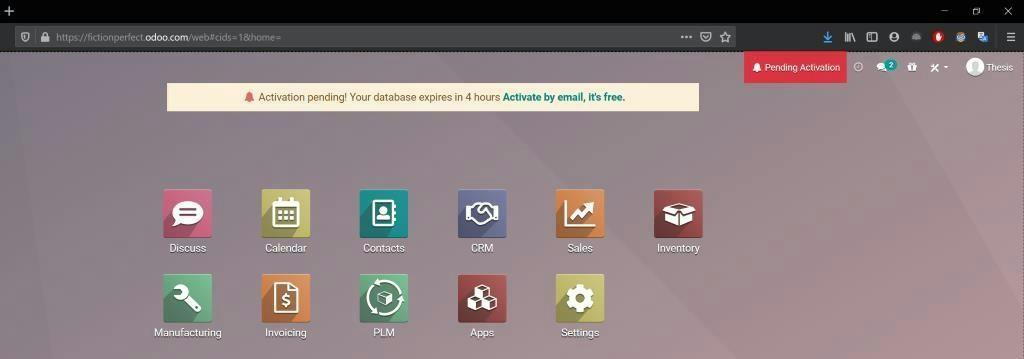
\includegraphics[width=445.32pt,height=156.15pt]{latexImage_cf2a7a0f230d4e58027581a48b41477a.png}}
\end{picture}
\newpage
\begin{tikzpicture}[overlay]\path(0pt,0pt);\end{tikzpicture}
\begin{picture}(-5,0)(2.5,0)
\put(500.26,-727.616){\fontsize{12}{1}\usefont{T1}{ptm}{m}{n}\selectfont\color{color_29791}27}
\put(511.78,-727.616){\fontsize{12}{1}\usefont{T1}{ptm}{m}{n}\selectfont\color{color_29791} }
\put(63.024,-726.896){\fontsize{9.96}{1}\usefont{T1}{ptm}{m}{n}\selectfont\color{color_29791} }
\put(82.944,-72.56){\fontsize{12}{1}\usefont{T1}{ptm}{m}{n}\selectfont\color{color_29791}從}
\put(94.82,-72.56){\fontsize{12}{1}\usefont{T1}{ptm}{m}{n}\selectfont\color{color_29791}O}
\put(103.34,-72.56){\fontsize{12}{1}\usefont{T1}{ptm}{m}{n}\selectfont\color{color_29791}d}
\put(109.22,-72.56){\fontsize{12}{1}\usefont{T1}{ptm}{m}{n}\selectfont\color{color_29791}o}
\put(115.1,-72.56){\fontsize{12}{1}\usefont{T1}{ptm}{m}{n}\selectfont\color{color_29791}o}
\put(120.98,-72.56){\fontsize{12}{1}\usefont{T1}{ptm}{m}{n}\selectfont\color{color_29791}的}
\put(132.86,-72.56){\fontsize{12}{1}\usefont{T1}{ptm}{m}{n}\selectfont\color{color_29791}角度}
\put(156.74,-72.56){\fontsize{12}{1}\usefont{T1}{ptm}{m}{n}\selectfont\color{color_29791}來}
\put(168.62,-72.56){\fontsize{12}{1}\usefont{T1}{ptm}{m}{n}\selectfont\color{color_29791}看}
\put(180.5,-72.56){\fontsize{12}{1}\usefont{T1}{ptm}{m}{n}\selectfont\color{color_29791},}
\put(192.38,-72.56){\fontsize{12}{1}\usefont{T1}{ptm}{m}{n}\selectfont\color{color_29791}在任}
\put(216.26,-72.56){\fontsize{12}{1}\usefont{T1}{ptm}{m}{n}\selectfont\color{color_29791}何}
\put(228.14,-72.56){\fontsize{12}{1}\usefont{T1}{ptm}{m}{n}\selectfont\color{color_29791}常}
\put(240.02,-72.56){\fontsize{12}{1}\usefont{T1}{ptm}{m}{n}\selectfont\color{color_29791}規}
\put(251.9,-72.56){\fontsize{12}{1}\usefont{T1}{ptm}{m}{n}\selectfont\color{color_29791}製}
\put(263.78,-72.56){\fontsize{12}{1}\usefont{T1}{ptm}{m}{n}\selectfont\color{color_29791}造}
\put(275.66,-72.56){\fontsize{12}{1}\usefont{T1}{ptm}{m}{n}\selectfont\color{color_29791}過}
\put(287.54,-72.56){\fontsize{12}{1}\usefont{T1}{ptm}{m}{n}\selectfont\color{color_29791}程的}
\put(311.42,-72.56){\fontsize{12}{1}\usefont{T1}{ptm}{m}{n}\selectfont\color{color_29791}開始}
\put(335.3,-72.56){\fontsize{12}{1}\usefont{T1}{ptm}{m}{n}\selectfont\color{color_29791},}
\put(347.1801,-72.56){\fontsize{12}{1}\usefont{T1}{ptm}{m}{n}\selectfont\color{color_29791}第}
\put(359.0601,-72.56){\fontsize{12}{1}\usefont{T1}{ptm}{m}{n}\selectfont\color{color_29791}一}
\put(370.9401,-72.56){\fontsize{12}{1}\usefont{T1}{ptm}{m}{n}\selectfont\color{color_29791}步}
\put(382.8201,-72.56){\fontsize{12}{1}\usefont{T1}{ptm}{m}{n}\selectfont\color{color_29791}將}
\put(394.7001,-72.56){\fontsize{12}{1}\usefont{T1}{ptm}{m}{n}\selectfont\color{color_29791}是}
\put(406.5801,-72.56){\fontsize{12}{1}\usefont{T1}{ptm}{m}{n}\selectfont\color{color_29791}工程}
\put(430.4601,-72.56){\fontsize{12}{1}\usefont{T1}{ptm}{m}{n}\selectfont\color{color_29791}師通}
\put(454.3401,-72.56){\fontsize{12}{1}\usefont{T1}{ptm}{m}{n}\selectfont\color{color_29791}常}
\put(466.2201,-72.56){\fontsize{12}{1}\usefont{T1}{ptm}{m}{n}\selectfont\color{color_29791}使}
\put(478.1001,-72.56){\fontsize{12}{1}\usefont{T1}{ptm}{m}{n}\selectfont\color{color_29791}用}
\put(490.06,-72.56){\fontsize{12}{1}\usefont{T1}{ptm}{m}{n}\selectfont\color{color_29791}C}
\put(497.98,-72.56){\fontsize{12}{1}\usefont{T1}{ptm}{m}{n}\selectfont\color{color_29791}A}
\put(506.5,-72.56){\fontsize{12}{1}\usefont{T1}{ptm}{m}{n}\selectfont\color{color_29791} }
\put(69.384,-90.34003){\fontsize{12}{1}\usefont{T1}{ptm}{m}{n}\selectfont\color{color_29791}D}
\put(77.904,-90.34003){\fontsize{12}{1}\usefont{T1}{ptm}{m}{n}\selectfont\color{color_29791}軟}
\put(89.784,-90.34003){\fontsize{12}{1}\usefont{T1}{ptm}{m}{n}\selectfont\color{color_29791}體}
\put(101.664,-90.34003){\fontsize{12}{1}\usefont{T1}{ptm}{m}{n}\selectfont\color{color_29791}設}
\put(113.544,-90.34003){\fontsize{12}{1}\usefont{T1}{ptm}{m}{n}\selectfont\color{color_29791}計}
\put(125.424,-90.34003){\fontsize{12}{1}\usefont{T1}{ptm}{m}{n}\selectfont\color{color_29791}產}
\put(137.304,-90.34003){\fontsize{12}{1}\usefont{T1}{ptm}{m}{n}\selectfont\color{color_29791}品。}
\put(161.184,-90.34003){\fontsize{12}{1}\usefont{T1}{ptm}{m}{n}\selectfont\color{color_29791}完}
\put(173.064,-90.34003){\fontsize{12}{1}\usefont{T1}{ptm}{m}{n}\selectfont\color{color_29791}成後}
\put(196.944,-90.34003){\fontsize{12}{1}\usefont{T1}{ptm}{m}{n}\selectfont\color{color_29791},}
\put(208.824,-90.34003){\fontsize{12}{1}\usefont{T1}{ptm}{m}{n}\selectfont\color{color_29791}他}
\put(220.704,-90.34003){\fontsize{12}{1}\usefont{T1}{ptm}{m}{n}\selectfont\color{color_29791}們}
\put(232.584,-90.34003){\fontsize{12}{1}\usefont{T1}{ptm}{m}{n}\selectfont\color{color_29791}將}
\put(244.464,-90.34003){\fontsize{12}{1}\usefont{T1}{ptm}{m}{n}\selectfont\color{color_29791}創}
\put(256.344,-90.34003){\fontsize{12}{1}\usefont{T1}{ptm}{m}{n}\selectfont\color{color_29791}建}
\put(268.224,-90.34003){\fontsize{12}{1}\usefont{T1}{ptm}{m}{n}\selectfont\color{color_29791}物料}
\put(292.104,-90.34003){\fontsize{12}{1}\usefont{T1}{ptm}{m}{n}\selectfont\color{color_29791}清單}
\put(316.03,-90.34003){\fontsize{12}{1}\usefont{T1}{ptm}{m}{n}\selectfont\color{color_29791} }
\put(69.384,-108.34){\fontsize{12}{1}\usefont{T1}{ptm}{m}{n}\selectfont\color{color_29791}(}
\put(81.264,-108.34){\fontsize{12}{1}\usefont{T1}{ptm}{m}{n}\selectfont\color{color_29791}B}
\put(89.184,-108.34){\fontsize{12}{1}\usefont{T1}{ptm}{m}{n}\selectfont\color{color_29791}O}
\put(97.70399,-108.34){\fontsize{12}{1}\usefont{T1}{ptm}{m}{n}\selectfont\color{color_29791}M}
\put(108.26,-108.34){\fontsize{12}{1}\usefont{T1}{ptm}{m}{n}\selectfont\color{color_29791})}
\put(120.14,-108.34){\fontsize{12}{1}\usefont{T1}{ptm}{m}{n}\selectfont\color{color_29791},}
\put(132.02,-108.34){\fontsize{12}{1}\usefont{T1}{ptm}{m}{n}\selectfont\color{color_29791}這}
\put(143.9,-108.34){\fontsize{12}{1}\usefont{T1}{ptm}{m}{n}\selectfont\color{color_29791}是}
\put(155.78,-108.34){\fontsize{12}{1}\usefont{T1}{ptm}{m}{n}\selectfont\color{color_29791}生產}
\put(179.66,-108.34){\fontsize{12}{1}\usefont{T1}{ptm}{m}{n}\selectfont\color{color_29791}產品}
\put(203.54,-108.34){\fontsize{12}{1}\usefont{T1}{ptm}{m}{n}\selectfont\color{color_29791}所}
\put(215.42,-108.34){\fontsize{12}{1}\usefont{T1}{ptm}{m}{n}\selectfont\color{color_29791}需}
\put(227.3,-108.34){\fontsize{12}{1}\usefont{T1}{ptm}{m}{n}\selectfont\color{color_29791}的}
\put(239.18,-108.34){\fontsize{12}{1}\usefont{T1}{ptm}{m}{n}\selectfont\color{color_29791}元}
\put(251.06,-108.34){\fontsize{12}{1}\usefont{T1}{ptm}{m}{n}\selectfont\color{color_29791}件}
\put(262.94,-108.34){\fontsize{12}{1}\usefont{T1}{ptm}{m}{n}\selectfont\color{color_29791}或}
\put(274.82,-108.34){\fontsize{12}{1}\usefont{T1}{ptm}{m}{n}\selectfont\color{color_29791}材料}
\put(298.7,-108.34){\fontsize{12}{1}\usefont{T1}{ptm}{m}{n}\selectfont\color{color_29791}清單}
\put(322.58,-108.34){\fontsize{12}{1}\usefont{T1}{ptm}{m}{n}\selectfont\color{color_29791}。}
\put(334.4601,-108.34){\fontsize{12}{1}\usefont{T1}{ptm}{m}{n}\selectfont\color{color_29791}在}
\put(346.3401,-108.34){\fontsize{12}{1}\usefont{T1}{ptm}{m}{n}\selectfont\color{color_29791}這}
\put(358.2201,-108.34){\fontsize{12}{1}\usefont{T1}{ptm}{m}{n}\selectfont\color{color_29791}一}
\put(370.1001,-108.34){\fontsize{12}{1}\usefont{T1}{ptm}{m}{n}\selectfont\color{color_29791}點}
\put(381.9801,-108.34){\fontsize{12}{1}\usefont{T1}{ptm}{m}{n}\selectfont\color{color_29791}上}
\put(393.8601,-108.34){\fontsize{12}{1}\usefont{T1}{ptm}{m}{n}\selectfont\color{color_29791},重}
\put(417.7401,-108.34){\fontsize{12}{1}\usefont{T1}{ptm}{m}{n}\selectfont\color{color_29791}點放}
\put(441.6201,-108.34){\fontsize{12}{1}\usefont{T1}{ptm}{m}{n}\selectfont\color{color_29791}在}
\put(453.5001,-108.34){\fontsize{12}{1}\usefont{T1}{ptm}{m}{n}\selectfont\color{color_29791}製}
\put(465.3801,-108.34){\fontsize{12}{1}\usefont{T1}{ptm}{m}{n}\selectfont\color{color_29791}造}
\put(477.2601,-108.34){\fontsize{12}{1}\usefont{T1}{ptm}{m}{n}\selectfont\color{color_29791}過}
\put(489.1401,-108.34){\fontsize{12}{1}\usefont{T1}{ptm}{m}{n}\selectfont\color{color_29791}程}
\put(69.384,-126.22){\fontsize{12}{1}\usefont{T1}{ptm}{m}{n}\selectfont\color{color_29791}本身。}
\put(104.78,-126.22){\fontsize{12}{1}\usefont{T1}{ptm}{m}{n}\selectfont\color{color_29791} }
\put(63.024,-144.34){\fontsize{12}{1}\usefont{T1}{ptm}{m}{n}\selectfont\color{color_29791} }
\put(82.944,-159.94){\fontsize{12}{1}\usefont{T1}{ptm}{m}{n}\selectfont\color{color_29791}流程的軟體檢視側重於}
\put(203.052,-159.94){\fontsize{12}{1}\usefont{T1}{ptm}{m}{n}\selectfont\color{color_29791}工藝路線、工作表和工}
\put(323.16,-159.94){\fontsize{12}{1}\usefont{T1}{ptm}{m}{n}\selectfont\color{color_29791}作中心,這是由製造工}
\put(443.268,-159.94){\fontsize{12}{1}\usefont{T1}{ptm}{m}{n}\selectfont\color{color_29791}程團隊完成}
\put(69.384,-177.82){\fontsize{12}{1}\usefont{T1}{ptm}{m}{n}\selectfont\color{color_29791}的。工}
\put(105.492,-177.82){\fontsize{12}{1}\usefont{T1}{ptm}{m}{n}\selectfont\color{color_29791}藝路}
\put(129.6,-177.82){\fontsize{12}{1}\usefont{T1}{ptm}{m}{n}\selectfont\color{color_29791}線是}
\put(153.708,-177.82){\fontsize{12}{1}\usefont{T1}{ptm}{m}{n}\selectfont\color{color_29791}產品在}
\put(189.816,-177.82){\fontsize{12}{1}\usefont{T1}{ptm}{m}{n}\selectfont\color{color_29791}生產過}
\put(225.924,-177.82){\fontsize{12}{1}\usefont{T1}{ptm}{m}{n}\selectfont\color{color_29791}程中}
\put(250.032,-177.82){\fontsize{12}{1}\usefont{T1}{ptm}{m}{n}\selectfont\color{color_29791}經歷}
\put(274.14,-177.82){\fontsize{12}{1}\usefont{T1}{ptm}{m}{n}\selectfont\color{color_29791}的一組}
\put(310.248,-177.82){\fontsize{12}{1}\usefont{T1}{ptm}{m}{n}\selectfont\color{color_29791}步驟。}
\put(346.356,-177.82){\fontsize{12}{1}\usefont{T1}{ptm}{m}{n}\selectfont\color{color_29791}工作}
\put(370.464,-177.82){\fontsize{12}{1}\usefont{T1}{ptm}{m}{n}\selectfont\color{color_29791}表是}
\put(394.572,-177.82){\fontsize{12}{1}\usefont{T1}{ptm}{m}{n}\selectfont\color{color_29791}製造操}
\put(430.68,-177.82){\fontsize{12}{1}\usefont{T1}{ptm}{m}{n}\selectfont\color{color_29791}作員的}
\put(466.788,-177.82){\fontsize{12}{1}\usefont{T1}{ptm}{m}{n}\selectfont\color{color_29791}指令}
\put(490.896,-177.82){\fontsize{12}{1}\usefont{T1}{ptm}{m}{n}\selectfont\color{color_29791},}
\put(69.384,-195.7){\fontsize{12}{1}\usefont{T1}{ptm}{m}{n}\selectfont\color{color_29791}工作中心是進行生}
\put(164.532,-195.7){\fontsize{12}{1}\usefont{T1}{ptm}{m}{n}\selectfont\color{color_29791}產的}
\put(188.4,-195.7){\fontsize{12}{1}\usefont{T1}{ptm}{m}{n}\selectfont\color{color_29791}地方。}
\put(224.09,-195.7){\fontsize{12}{1}\usefont{T1}{ptm}{m}{n}\selectfont\color{color_29791}O}
\put(232.61,-195.7){\fontsize{12}{1}\usefont{T1}{ptm}{m}{n}\selectfont\color{color_29791}d}
\put(238.49,-195.7){\fontsize{12}{1}\usefont{T1}{ptm}{m}{n}\selectfont\color{color_29791}o}
\put(244.37,-195.7){\fontsize{12}{1}\usefont{T1}{ptm}{m}{n}\selectfont\color{color_29791}o}
\put(250.37,-195.7){\fontsize{12}{1}\usefont{T1}{ptm}{m}{n}\selectfont\color{color_29791}認}
\put(262.25,-195.7){\fontsize{12}{1}\usefont{T1}{ptm}{m}{n}\selectfont\color{color_29791}為}
\put(274.13,-195.7){\fontsize{12}{1}\usefont{T1}{ptm}{m}{n}\selectfont\color{color_29791}這}
\put(286.01,-195.7){\fontsize{12}{1}\usefont{T1}{ptm}{m}{n}\selectfont\color{color_29791}些}
\put(297.89,-195.7){\fontsize{12}{1}\usefont{T1}{ptm}{m}{n}\selectfont\color{color_29791}是將}
\put(321.77,-195.7){\fontsize{12}{1}\usefont{T1}{ptm}{m}{n}\selectfont\color{color_29791}工}
\put(333.65,-195.7){\fontsize{12}{1}\usefont{T1}{ptm}{m}{n}\selectfont\color{color_29791}程}
\put(345.53,-195.7){\fontsize{12}{1}\usefont{T1}{ptm}{m}{n}\selectfont\color{color_29791}師}
\put(357.41,-195.7){\fontsize{12}{1}\usefont{T1}{ptm}{m}{n}\selectfont\color{color_29791}計}
\put(369.29,-195.7){\fontsize{12}{1}\usefont{T1}{ptm}{m}{n}\selectfont\color{color_29791}劃}
\put(381.17,-195.7){\fontsize{12}{1}\usefont{T1}{ptm}{m}{n}\selectfont\color{color_29791}付}
\put(393.05,-195.7){\fontsize{12}{1}\usefont{T1}{ptm}{m}{n}\selectfont\color{color_29791}諸實}
\put(416.9301,-195.7){\fontsize{12}{1}\usefont{T1}{ptm}{m}{n}\selectfont\color{color_29791}施的}
\put(440.8101,-195.7){\fontsize{12}{1}\usefont{T1}{ptm}{m}{n}\selectfont\color{color_29791}要}
\put(452.6901,-195.7){\fontsize{12}{1}\usefont{T1}{ptm}{m}{n}\selectfont\color{color_29791}求}
\put(464.74,-195.7){\fontsize{12}{1}\usefont{T1}{ptm}{m}{n}\selectfont\color{color_29791} }
\put(63.024,-213.94){\fontsize{12}{1}\usefont{T1}{ptm}{m}{n}\selectfont\color{color_29791} }
\put(82.944,-229.42){\fontsize{12}{1}\usefont{T1}{ptm}{m}{n}\selectfont\color{color_29791}採購部門將負責詢}
\put(178.94,-229.42){\fontsize{12}{1}\usefont{T1}{ptm}{m}{n}\selectfont\color{color_29791}價}
\put(190.49,-229.42){\fontsize{12}{1}\usefont{T1}{ptm}{m}{n}\selectfont\color{color_29791} }
\put(298.01,-229.42){\fontsize{12}{1}\usefont{T1}{ptm}{m}{n}\selectfont\color{color_29791}(}
\put(309.91,-229.42){\fontsize{12}{1}\usefont{T1}{ptm}{m}{n}\selectfont\color{color_29791}R}
\put(317.83,-229.42){\fontsize{12}{1}\usefont{T1}{ptm}{m}{n}\selectfont\color{color_29791}F}
\put(324.31,-229.42){\fontsize{12}{1}\usefont{T1}{ptm}{m}{n}\selectfont\color{color_29791}Q}
\put(332.83,-229.42){\fontsize{12}{1}\usefont{T1}{ptm}{m}{n}\selectfont\color{color_29791})}
\put(344.83,-229.42){\fontsize{12}{1}\usefont{T1}{ptm}{m}{n}\selectfont\color{color_29791} }
\put(452.5,-229.42){\fontsize{12}{1}\usefont{T1}{ptm}{m}{n}\selectfont\color{color_29791}或採購訂}
\put(500.5,-229.42){\fontsize{12}{1}\usefont{T1}{ptm}{m}{n}\selectfont\color{color_29791}單}
\put(512.02,-229.42){\fontsize{12}{1}\usefont{T1}{ptm}{m}{n}\selectfont\color{color_29791} }
\put(69.384,-247.33){\fontsize{12}{1}\usefont{T1}{ptm}{m}{n}\selectfont\color{color_29791}(}
\put(81.384,-247.33){\fontsize{12}{1}\usefont{T1}{ptm}{m}{n}\selectfont\color{color_29791}P}
\put(88.1,-247.33){\fontsize{12}{1}\usefont{T1}{ptm}{m}{n}\selectfont\color{color_29791}O}
\put(96.74,-247.33){\fontsize{12}{1}\usefont{T1}{ptm}{m}{n}\selectfont\color{color_29791})。庫存操作員}
\put(180.62,-247.33){\fontsize{12}{1}\usefont{T1}{ptm}{m}{n}\selectfont\color{color_29791}根據這些採購訂單處理收據,這通常是使用}
\put(408.67,-247.33){\fontsize{12}{1}\usefont{T1}{ptm}{m}{n}\selectfont\color{color_29791}Odo}
\put(429.31,-247.33){\fontsize{12}{1}\usefont{T1}{ptm}{m}{n}\selectfont\color{color_29791}o}
\put(435.31,-247.33){\fontsize{12}{1}\usefont{T1}{ptm}{m}{n}\selectfont\color{color_29791}中的條碼應用}
\put(69.384,-265.33){\fontsize{12}{1}\usefont{T1}{ptm}{m}{n}\selectfont\color{color_29791}程式完}
\put(105.264,-265.33){\fontsize{12}{1}\usefont{T1}{ptm}{m}{n}\selectfont\color{color_29791}成的。}
\put(141.144,-265.33){\fontsize{12}{1}\usefont{T1}{ptm}{m}{n}\selectfont\color{color_29791}如本}
\put(165.024,-265.33){\fontsize{12}{1}\usefont{T1}{ptm}{m}{n}\selectfont\color{color_29791}章第}
\put(188.904,-265.33){\fontsize{12}{1}\usefont{T1}{ptm}{m}{n}\selectfont\color{color_29791}一節所}
\put(224.784,-265.33){\fontsize{12}{1}\usefont{T1}{ptm}{m}{n}\selectfont\color{color_29791}述,}
\put(248.81,-265.33){\fontsize{12}{1}\usefont{T1}{ptm}{m}{n}\selectfont\color{color_29791}Odo}
\put(269.45,-265.33){\fontsize{12}{1}\usefont{T1}{ptm}{m}{n}\selectfont\color{color_29791}o}
\put(275.45,-265.33){\fontsize{12}{1}\usefont{T1}{ptm}{m}{n}\selectfont\color{color_29791}主要是}
\put(311.33,-265.33){\fontsize{12}{1}\usefont{T1}{ptm}{m}{n}\selectfont\color{color_29791}一個}
\put(335.35,-265.33){\fontsize{12}{1}\usefont{T1}{ptm}{m}{n}\selectfont\color{color_29791}ER}
\put(350.71,-265.33){\fontsize{12}{1}\usefont{T1}{ptm}{m}{n}\selectfont\color{color_29791}P}
\put(357.43,-265.33){\fontsize{12}{1}\usefont{T1}{ptm}{m}{n}\selectfont\color{color_29791}系}
\put(369.31,-265.33){\fontsize{12}{1}\usefont{T1}{ptm}{m}{n}\selectfont\color{color_29791}統,}
\put(393.19,-265.33){\fontsize{12}{1}\usefont{T1}{ptm}{m}{n}\selectfont\color{color_29791}在這一}
\put(429.07,-265.33){\fontsize{12}{1}\usefont{T1}{ptm}{m}{n}\selectfont\color{color_29791}點上,}
\put(464.95,-265.33){\fontsize{12}{1}\usefont{T1}{ptm}{m}{n}\selectfont\color{color_29791}可以注}
\put(69.384,-283.21){\fontsize{12}{1}\usefont{T1}{ptm}{m}{n}\selectfont\color{color_29791}意到一}
\put(105.264,-283.21){\fontsize{12}{1}\usefont{T1}{ptm}{m}{n}\selectfont\color{color_29791}些以}
\put(129.26,-283.21){\fontsize{12}{1}\usefont{T1}{ptm}{m}{n}\selectfont\color{color_29791}ER}
\put(144.5,-283.21){\fontsize{12}{1}\usefont{T1}{ptm}{m}{n}\selectfont\color{color_29791}P}
\put(151.22,-283.21){\fontsize{12}{1}\usefont{T1}{ptm}{m}{n}\selectfont\color{color_29791}為}
\put(163.1,-283.21){\fontsize{12}{1}\usefont{T1}{ptm}{m}{n}\selectfont\color{color_29791}中}
\put(174.98,-283.21){\fontsize{12}{1}\usefont{T1}{ptm}{m}{n}\selectfont\color{color_29791}心}
\put(186.74,-283.21){\fontsize{12}{1}\usefont{T1}{ptm}{m}{n}\selectfont\color{color_29791}的}
\put(198.62,-283.21){\fontsize{12}{1}\usefont{T1}{ptm}{m}{n}\selectfont\color{color_29791}特}
\put(210.5,-283.21){\fontsize{12}{1}\usefont{T1}{ptm}{m}{n}\selectfont\color{color_29791}徵}
\put(222.38,-283.21){\fontsize{12}{1}\usefont{T1}{ptm}{m}{n}\selectfont\color{color_29791},}
\put(234.26,-283.21){\fontsize{12}{1}\usefont{T1}{ptm}{m}{n}\selectfont\color{color_29791}例}
\put(246.14,-283.21){\fontsize{12}{1}\usefont{T1}{ptm}{m}{n}\selectfont\color{color_29791}如}
\put(258.02,-283.21){\fontsize{12}{1}\usefont{T1}{ptm}{m}{n}\selectfont\color{color_29791}對}
\put(269.9,-283.21){\fontsize{12}{1}\usefont{T1}{ptm}{m}{n}\selectfont\color{color_29791}庫存}
\put(293.78,-283.21){\fontsize{12}{1}\usefont{T1}{ptm}{m}{n}\selectfont\color{color_29791}和資}
\put(317.66,-283.21){\fontsize{12}{1}\usefont{T1}{ptm}{m}{n}\selectfont\color{color_29791}源}
\put(329.54,-283.21){\fontsize{12}{1}\usefont{T1}{ptm}{m}{n}\selectfont\color{color_29791}管}
\put(341.42,-283.21){\fontsize{12}{1}\usefont{T1}{ptm}{m}{n}\selectfont\color{color_29791}理}
\put(353.3,-283.21){\fontsize{12}{1}\usefont{T1}{ptm}{m}{n}\selectfont\color{color_29791}的}
\put(365.1801,-283.21){\fontsize{12}{1}\usefont{T1}{ptm}{m}{n}\selectfont\color{color_29791}關}
\put(377.0601,-283.21){\fontsize{12}{1}\usefont{T1}{ptm}{m}{n}\selectfont\color{color_29791}注}
\put(388.9401,-283.21){\fontsize{12}{1}\usefont{T1}{ptm}{m}{n}\selectfont\color{color_29791}。這}
\put(412.8201,-283.21){\fontsize{12}{1}\usefont{T1}{ptm}{m}{n}\selectfont\color{color_29791}將在}
\put(436.7001,-283.21){\fontsize{12}{1}\usefont{T1}{ptm}{m}{n}\selectfont\color{color_29791}以}
\put(448.5801,-283.21){\fontsize{12}{1}\usefont{T1}{ptm}{m}{n}\selectfont\color{color_29791}下}
\put(460.4601,-283.21){\fontsize{12}{1}\usefont{T1}{ptm}{m}{n}\selectfont\color{color_29791}各}
\put(472.3401,-283.21){\fontsize{12}{1}\usefont{T1}{ptm}{m}{n}\selectfont\color{color_29791}節}
\put(484.2201,-283.21){\fontsize{12}{1}\usefont{T1}{ptm}{m}{n}\selectfont\color{color_29791}中}
\put(496.1001,-283.21){\fontsize{12}{1}\usefont{T1}{ptm}{m}{n}\selectfont\color{color_29791}進}
\put(69.384,-301.09){\fontsize{12}{1}\usefont{T1}{ptm}{m}{n}\selectfont\color{color_29791}一步分析,但公平地指}
\put(186.864,-301.09){\fontsize{12}{1}\usefont{T1}{ptm}{m}{n}\selectfont\color{color_29791}出,這些}
\put(233.93,-301.09){\fontsize{12}{1}\usefont{T1}{ptm}{m}{n}\selectfont\color{color_29791} }
\put(239.69,-301.09){\fontsize{12}{1}\usefont{T1}{ptm}{m}{n}\selectfont\color{color_29791}R}
\put(247.73,-301.09){\fontsize{12}{1}\usefont{T1}{ptm}{m}{n}\selectfont\color{color_29791}F}
\put(254.21,-301.09){\fontsize{12}{1}\usefont{T1}{ptm}{m}{n}\selectfont\color{color_29791}Q}
\put(262.85,-301.09){\fontsize{12}{1}\usefont{T1}{ptm}{m}{n}\selectfont\color{color_29791} }
\put(265.85,-301.09){\fontsize{12}{1}\usefont{T1}{ptm}{m}{n}\selectfont\color{color_29791}和}
\put(276.29,-301.09){\fontsize{12}{1}\usefont{T1}{ptm}{m}{n}\selectfont\color{color_29791} }
\put(280.73,-301.09){\fontsize{12}{1}\usefont{T1}{ptm}{m}{n}\selectfont\color{color_29791}PO}
\put(296.09,-301.09){\fontsize{12}{1}\usefont{T1}{ptm}{m}{n}\selectfont\color{color_29791} }
\put(299.09,-301.09){\fontsize{12}{1}\usefont{T1}{ptm}{m}{n}\selectfont\color{color_29791}被視為資料庫中的專案。}
\put(431.11,-301.09){\fontsize{12}{1}\usefont{T1}{ptm}{m}{n}\selectfont\color{color_29791} }
\put(63.024,-319.21){\fontsize{12}{1}\usefont{T1}{ptm}{m}{n}\selectfont\color{color_29791} }
\put(82.944,-334.81){\fontsize{12}{1}\usefont{T1}{ptm}{m}{n}\selectfont\color{color_29791}只有當您擁有所需}
\put(178.092,-334.81){\fontsize{12}{1}\usefont{T1}{ptm}{m}{n}\selectfont\color{color_29791}的設}
\put(201.96,-334.81){\fontsize{12}{1}\usefont{T1}{ptm}{m}{n}\selectfont\color{color_29791}計、工藝和材料時}
\put(297.108,-334.81){\fontsize{12}{1}\usefont{T1}{ptm}{m}{n}\selectfont\color{color_29791},}
\put(309.07,-334.81){\fontsize{12}{1}\usefont{T1}{ptm}{m}{n}\selectfont\color{color_29791}O}
\put(317.59,-334.81){\fontsize{12}{1}\usefont{T1}{ptm}{m}{n}\selectfont\color{color_29791}do}
\put(329.47,-334.81){\fontsize{12}{1}\usefont{T1}{ptm}{m}{n}\selectfont\color{color_29791}o}
\put(335.35,-334.81){\fontsize{12}{1}\usefont{T1}{ptm}{m}{n}\selectfont\color{color_29791}才}
\put(347.23,-334.81){\fontsize{12}{1}\usefont{T1}{ptm}{m}{n}\selectfont\color{color_29791}會}
\put(359.11,-334.81){\fontsize{12}{1}\usefont{T1}{ptm}{m}{n}\selectfont\color{color_29791}考}
\put(370.99,-334.81){\fontsize{12}{1}\usefont{T1}{ptm}{m}{n}\selectfont\color{color_29791}慮}
\put(382.87,-334.81){\fontsize{12}{1}\usefont{T1}{ptm}{m}{n}\selectfont\color{color_29791}製}
\put(394.75,-334.81){\fontsize{12}{1}\usefont{T1}{ptm}{m}{n}\selectfont\color{color_29791}造。}
\put(418.63,-334.81){\fontsize{12}{1}\usefont{T1}{ptm}{m}{n}\selectfont\color{color_29791}然}
\put(430.51,-334.81){\fontsize{12}{1}\usefont{T1}{ptm}{m}{n}\selectfont\color{color_29791}後,}
\put(454.39,-334.81){\fontsize{12}{1}\usefont{T1}{ptm}{m}{n}\selectfont\color{color_29791}製}
\put(466.2701,-334.81){\fontsize{12}{1}\usefont{T1}{ptm}{m}{n}\selectfont\color{color_29791}造}
\put(478.1501,-334.81){\fontsize{12}{1}\usefont{T1}{ptm}{m}{n}\selectfont\color{color_29791}領}
\put(490.0301,-334.81){\fontsize{12}{1}\usefont{T1}{ptm}{m}{n}\selectfont\color{color_29791}班}
\put(69.384,-352.57){\fontsize{12}{1}\usefont{T1}{ptm}{m}{n}\selectfont\color{color_29791}將創建製造訂單}
\put(152.66,-352.57){\fontsize{12}{1}\usefont{T1}{ptm}{m}{n}\selectfont\color{color_29791} }
\put(216.05,-352.57){\fontsize{12}{1}\usefont{T1}{ptm}{m}{n}\selectfont\color{color_29791}(}
\put(227.81,-352.57){\fontsize{12}{1}\usefont{T1}{ptm}{m}{n}\selectfont\color{color_29791}MO}
\put(246.65,-352.57){\fontsize{12}{1}\usefont{T1}{ptm}{m}{n}\selectfont\color{color_29791})}
\put(258.53,-352.57){\fontsize{12}{1}\usefont{T1}{ptm}{m}{n}\selectfont\color{color_29791} }
\put(322.03,-352.57){\fontsize{12}{1}\usefont{T1}{ptm}{m}{n}\selectfont\color{color_29791}並通過工作訂單}
\put(405.31,-352.57){\fontsize{12}{1}\usefont{T1}{ptm}{m}{n}\selectfont\color{color_29791} }
\put(468.7,-352.57){\fontsize{12}{1}\usefont{T1}{ptm}{m}{n}\selectfont\color{color_29791}(}
\put(480.46,-352.57){\fontsize{12}{1}\usefont{T1}{ptm}{m}{n}\selectfont\color{color_29791}WO}
\put(500.02,-352.57){\fontsize{12}{1}\usefont{T1}{ptm}{m}{n}\selectfont\color{color_29791})}
\put(69.384,-370.21){\fontsize{12}{1}\usefont{T1}{ptm}{m}{n}\selectfont\color{color_29791}和工作中心管理製}
\put(164.532,-370.21){\fontsize{12}{1}\usefont{T1}{ptm}{m}{n}\selectfont\color{color_29791}造操}
\put(188.4,-370.21){\fontsize{12}{1}\usefont{T1}{ptm}{m}{n}\selectfont\color{color_29791}作員的計劃。然後}
\put(283.548,-370.21){\fontsize{12}{1}\usefont{T1}{ptm}{m}{n}\selectfont\color{color_29791},製}
\put(307.416,-370.21){\fontsize{12}{1}\usefont{T1}{ptm}{m}{n}\selectfont\color{color_29791}造操作員可以按照}
\put(402.564,-370.21){\fontsize{12}{1}\usefont{T1}{ptm}{m}{n}\selectfont\color{color_29791}工作}
\put(426.432,-370.21){\fontsize{12}{1}\usefont{T1}{ptm}{m}{n}\selectfont\color{color_29791}訂單開始生產}
\put(497.98,-370.21){\fontsize{12}{1}\usefont{T1}{ptm}{m}{n}\selectfont\color{color_29791} }
\put(69.384,-388.21){\fontsize{12}{1}\usefont{T1}{ptm}{m}{n}\selectfont\color{color_29791}。產品生產完成後}
\put(164.532,-388.21){\fontsize{12}{1}\usefont{T1}{ptm}{m}{n}\selectfont\color{color_29791},它}
\put(188.4,-388.21){\fontsize{12}{1}\usefont{T1}{ptm}{m}{n}\selectfont\color{color_29791}們會自動出現在庫}
\put(283.548,-388.21){\fontsize{12}{1}\usefont{T1}{ptm}{m}{n}\selectfont\color{color_29791}存資}
\put(307.416,-388.21){\fontsize{12}{1}\usefont{T1}{ptm}{m}{n}\selectfont\color{color_29791}料庫中,該資料庫}
\put(402.564,-388.21){\fontsize{12}{1}\usefont{T1}{ptm}{m}{n}\selectfont\color{color_29791}與包}
\put(426.432,-388.21){\fontsize{12}{1}\usefont{T1}{ptm}{m}{n}\selectfont\color{color_29791}裝和交付一起}
\put(69.384,-406.21){\fontsize{12}{1}\usefont{T1}{ptm}{m}{n}\selectfont\color{color_29791}由庫存部門管理。}
\put(164.54,-406.21){\fontsize{12}{1}\usefont{T1}{ptm}{m}{n}\selectfont\color{color_29791} }
\put(63.024,-424.23){\fontsize{12}{1}\usefont{T1}{ptm}{m}{n}\selectfont\color{color_29791} }
\put(82.944,-439.83){\fontsize{12}{1}\usefont{T1}{ptm}{m}{n}\selectfont\color{color_29791}O}
\put(91.464,-439.83){\fontsize{12}{1}\usefont{T1}{ptm}{m}{n}\selectfont\color{color_29791}d}
\put(97.344,-439.83){\fontsize{12}{1}\usefont{T1}{ptm}{m}{n}\selectfont\color{color_29791}o}
\put(103.224,-439.83){\fontsize{12}{1}\usefont{T1}{ptm}{m}{n}\selectfont\color{color_29791}o}
\put(109.1,-439.83){\fontsize{12}{1}\usefont{T1}{ptm}{m}{n}\selectfont\color{color_29791}認}
\put(120.98,-439.83){\fontsize{12}{1}\usefont{T1}{ptm}{m}{n}\selectfont\color{color_29791}為}
\put(132.86,-439.83){\fontsize{12}{1}\usefont{T1}{ptm}{m}{n}\selectfont\color{color_29791}質量}
\put(156.74,-439.83){\fontsize{12}{1}\usefont{T1}{ptm}{m}{n}\selectfont\color{color_29791}團}
\put(168.62,-439.83){\fontsize{12}{1}\usefont{T1}{ptm}{m}{n}\selectfont\color{color_29791}隊}
\put(180.5,-439.83){\fontsize{12}{1}\usefont{T1}{ptm}{m}{n}\selectfont\color{color_29791}負}
\put(192.38,-439.83){\fontsize{12}{1}\usefont{T1}{ptm}{m}{n}\selectfont\color{color_29791}責分}
\put(216.26,-439.83){\fontsize{12}{1}\usefont{T1}{ptm}{m}{n}\selectfont\color{color_29791}配}
\put(228.14,-439.83){\fontsize{12}{1}\usefont{T1}{ptm}{m}{n}\selectfont\color{color_29791}控}
\put(240.02,-439.83){\fontsize{12}{1}\usefont{T1}{ptm}{m}{n}\selectfont\color{color_29791}制}
\put(251.93,-439.83){\fontsize{12}{1}\usefont{T1}{ptm}{m}{n}\selectfont\color{color_29791}/}
\put(255.17,-439.83){\fontsize{12}{1}\usefont{T1}{ptm}{m}{n}\selectfont\color{color_29791}檢}
\put(267.05,-439.83){\fontsize{12}{1}\usefont{T1}{ptm}{m}{n}\selectfont\color{color_29791}查}
\put(278.93,-439.83){\fontsize{12}{1}\usefont{T1}{ptm}{m}{n}\selectfont\color{color_29791}點}
\put(290.81,-439.83){\fontsize{12}{1}\usefont{T1}{ptm}{m}{n}\selectfont\color{color_29791},並}
\put(314.69,-439.83){\fontsize{12}{1}\usefont{T1}{ptm}{m}{n}\selectfont\color{color_29791}識別}
\put(338.57,-439.83){\fontsize{12}{1}\usefont{T1}{ptm}{m}{n}\selectfont\color{color_29791}產}
\put(350.45,-439.83){\fontsize{12}{1}\usefont{T1}{ptm}{m}{n}\selectfont\color{color_29791}品}
\put(362.33,-439.83){\fontsize{12}{1}\usefont{T1}{ptm}{m}{n}\selectfont\color{color_29791}或}
\put(374.2101,-439.83){\fontsize{12}{1}\usefont{T1}{ptm}{m}{n}\selectfont\color{color_29791}生}
\put(386.0901,-439.83){\fontsize{12}{1}\usefont{T1}{ptm}{m}{n}\selectfont\color{color_29791}產}
\put(397.9701,-439.83){\fontsize{12}{1}\usefont{T1}{ptm}{m}{n}\selectfont\color{color_29791}中}
\put(409.8501,-439.83){\fontsize{12}{1}\usefont{T1}{ptm}{m}{n}\selectfont\color{color_29791}可能}
\put(433.7301,-439.83){\fontsize{12}{1}\usefont{T1}{ptm}{m}{n}\selectfont\color{color_29791}存在}
\put(457.6101,-439.83){\fontsize{12}{1}\usefont{T1}{ptm}{m}{n}\selectfont\color{color_29791}的}
\put(469.4901,-439.83){\fontsize{12}{1}\usefont{T1}{ptm}{m}{n}\selectfont\color{color_29791}問}
\put(481.3701,-439.83){\fontsize{12}{1}\usefont{T1}{ptm}{m}{n}\selectfont\color{color_29791}題}
\put(493.2501,-439.83){\fontsize{12}{1}\usefont{T1}{ptm}{m}{n}\selectfont\color{color_29791}。}
\put(69.384,-457.83){\fontsize{12}{1}\usefont{T1}{ptm}{m}{n}\selectfont\color{color_29791}從}
\put(81.264,-457.83){\fontsize{12}{1}\usefont{T1}{ptm}{m}{n}\selectfont\color{color_29791}M}
\put(91.824,-457.83){\fontsize{12}{1}\usefont{T1}{ptm}{m}{n}\selectfont\color{color_29791}E}
\put(99.02399,-457.83){\fontsize{12}{1}\usefont{T1}{ptm}{m}{n}\selectfont\color{color_29791}S}
\put(105.62,-457.83){\fontsize{12}{1}\usefont{T1}{ptm}{m}{n}\selectfont\color{color_29791}的}
\put(117.5,-457.83){\fontsize{12}{1}\usefont{T1}{ptm}{m}{n}\selectfont\color{color_29791}角}
\put(129.38,-457.83){\fontsize{12}{1}\usefont{T1}{ptm}{m}{n}\selectfont\color{color_29791}度}
\put(141.26,-457.83){\fontsize{12}{1}\usefont{T1}{ptm}{m}{n}\selectfont\color{color_29791}來}
\put(153.14,-457.83){\fontsize{12}{1}\usefont{T1}{ptm}{m}{n}\selectfont\color{color_29791}看}
\put(165.02,-457.83){\fontsize{12}{1}\usefont{T1}{ptm}{m}{n}\selectfont\color{color_29791},這些}
\put(200.9,-457.83){\fontsize{12}{1}\usefont{T1}{ptm}{m}{n}\selectfont\color{color_29791}品}
\put(212.78,-457.83){\fontsize{12}{1}\usefont{T1}{ptm}{m}{n}\selectfont\color{color_29791}質}
\put(224.66,-457.83){\fontsize{12}{1}\usefont{T1}{ptm}{m}{n}\selectfont\color{color_29791}控}
\put(236.54,-457.83){\fontsize{12}{1}\usefont{T1}{ptm}{m}{n}\selectfont\color{color_29791}制}
\put(248.42,-457.83){\fontsize{12}{1}\usefont{T1}{ptm}{m}{n}\selectfont\color{color_29791}檢}
\put(260.3,-457.83){\fontsize{12}{1}\usefont{T1}{ptm}{m}{n}\selectfont\color{color_29791}查}
\put(272.1801,-457.83){\fontsize{12}{1}\usefont{T1}{ptm}{m}{n}\selectfont\color{color_29791}點非}
\put(296.0601,-457.83){\fontsize{12}{1}\usefont{T1}{ptm}{m}{n}\selectfont\color{color_29791}常有}
\put(319.9401,-457.83){\fontsize{12}{1}\usefont{T1}{ptm}{m}{n}\selectfont\color{color_29791}趣}
\put(331.8201,-457.83){\fontsize{12}{1}\usefont{T1}{ptm}{m}{n}\selectfont\color{color_29791},}
\put(343.7001,-457.83){\fontsize{12}{1}\usefont{T1}{ptm}{m}{n}\selectfont\color{color_29791}因}
\put(355.5801,-457.83){\fontsize{12}{1}\usefont{T1}{ptm}{m}{n}\selectfont\color{color_29791}為}
\put(367.4601,-457.83){\fontsize{12}{1}\usefont{T1}{ptm}{m}{n}\selectfont\color{color_29791}它}
\put(379.3401,-457.83){\fontsize{12}{1}\usefont{T1}{ptm}{m}{n}\selectfont\color{color_29791}代}
\put(391.2201,-457.83){\fontsize{12}{1}\usefont{T1}{ptm}{m}{n}\selectfont\color{color_29791}表了}
\put(415.1001,-457.83){\fontsize{12}{1}\usefont{T1}{ptm}{m}{n}\selectfont\color{color_29791}在生}
\put(438.9801,-457.83){\fontsize{12}{1}\usefont{T1}{ptm}{m}{n}\selectfont\color{color_29791}產}
\put(450.8601,-457.83){\fontsize{12}{1}\usefont{T1}{ptm}{m}{n}\selectfont\color{color_29791}過}
\put(462.7401,-457.83){\fontsize{12}{1}\usefont{T1}{ptm}{m}{n}\selectfont\color{color_29791}程}
\put(474.6201,-457.83){\fontsize{12}{1}\usefont{T1}{ptm}{m}{n}\selectfont\color{color_29791}中}
\put(486.5001,-457.83){\fontsize{12}{1}\usefont{T1}{ptm}{m}{n}\selectfont\color{color_29791}即}
\put(69.384,-475.71){\fontsize{12}{1}\usefont{T1}{ptm}{m}{n}\selectfont\color{color_29791}時收集的有價值的}
\put(164.532,-475.71){\fontsize{12}{1}\usefont{T1}{ptm}{m}{n}\selectfont\color{color_29791}生產}
\put(188.4,-475.71){\fontsize{12}{1}\usefont{T1}{ptm}{m}{n}\selectfont\color{color_29791}數據,即,可以在}
\put(283.548,-475.71){\fontsize{12}{1}\usefont{T1}{ptm}{m}{n}\selectfont\color{color_29791}每件}
\put(307.416,-475.71){\fontsize{12}{1}\usefont{T1}{ptm}{m}{n}\selectfont\color{color_29791}作品生產後分配尺}
\put(402.564,-475.71){\fontsize{12}{1}\usefont{T1}{ptm}{m}{n}\selectfont\color{color_29791}寸檢}
\put(426.432,-475.71){\fontsize{12}{1}\usefont{T1}{ptm}{m}{n}\selectfont\color{color_29791}查,機械師將}
\put(69.384,-493.59){\fontsize{12}{1}\usefont{T1}{ptm}{m}{n}\selectfont\color{color_29791}填寫尺寸以跟蹤品}
\put(164.532,-493.59){\fontsize{12}{1}\usefont{T1}{ptm}{m}{n}\selectfont\color{color_29791}質隨}
\put(188.4,-493.59){\fontsize{12}{1}\usefont{T1}{ptm}{m}{n}\selectfont\color{color_29791}時間推移。}
\put(247.97,-493.59){\fontsize{12}{1}\usefont{T1}{ptm}{m}{n}\selectfont\color{color_29791} }
\put(63.024,-511.71){\fontsize{12}{1}\usefont{T1}{ptm}{m}{n}\selectfont\color{color_29791} }
\put(82.944,-527.31){\fontsize{12}{1}\usefont{T1}{ptm}{m}{n}\selectfont\color{color_29791}如果是}
\put(118.824,-527.31){\fontsize{12}{1}\usefont{T1}{ptm}{m}{n}\selectfont\color{color_29791}設計問}
\put(154.704,-527.31){\fontsize{12}{1}\usefont{T1}{ptm}{m}{n}\selectfont\color{color_29791}題或}
\put(178.584,-527.31){\fontsize{12}{1}\usefont{T1}{ptm}{m}{n}\selectfont\color{color_29791}有改}
\put(202.464,-527.31){\fontsize{12}{1}\usefont{T1}{ptm}{m}{n}\selectfont\color{color_29791}進的可}
\put(238.344,-527.31){\fontsize{12}{1}\usefont{T1}{ptm}{m}{n}\selectfont\color{color_29791}能性,}
\put(274.224,-527.31){\fontsize{12}{1}\usefont{T1}{ptm}{m}{n}\selectfont\color{color_29791}可以}
\put(298.104,-527.31){\fontsize{12}{1}\usefont{T1}{ptm}{m}{n}\selectfont\color{color_29791}發出}
\put(321.984,-527.31){\fontsize{12}{1}\usefont{T1}{ptm}{m}{n}\selectfont\color{color_29791}工程變}
\put(357.864,-527.31){\fontsize{12}{1}\usefont{T1}{ptm}{m}{n}\selectfont\color{color_29791}更單}
\put(381.79,-527.31){\fontsize{12}{1}\usefont{T1}{ptm}{m}{n}\selectfont\color{color_29791} }
\put(69.384,-545.19){\fontsize{12}{1}\usefont{T1}{ptm}{m}{n}\selectfont\color{color_29791}(}
\put(81.264,-545.19){\fontsize{12}{1}\usefont{T1}{ptm}{m}{n}\selectfont\color{color_29791}E}
\put(88.464,-545.19){\fontsize{12}{1}\usefont{T1}{ptm}{m}{n}\selectfont\color{color_29791}C}
\put(96.384,-545.19){\fontsize{12}{1}\usefont{T1}{ptm}{m}{n}\selectfont\color{color_29791}O}
\put(104.9,-545.19){\fontsize{12}{1}\usefont{T1}{ptm}{m}{n}\selectfont\color{color_29791})}
\put(116.78,-545.19){\fontsize{12}{1}\usefont{T1}{ptm}{m}{n}\selectfont\color{color_29791}。}
\put(128.66,-545.19){\fontsize{12}{1}\usefont{T1}{ptm}{m}{n}\selectfont\color{color_29791}這}
\put(140.54,-545.19){\fontsize{12}{1}\usefont{T1}{ptm}{m}{n}\selectfont\color{color_29791}又}
\put(152.42,-545.19){\fontsize{12}{1}\usefont{T1}{ptm}{m}{n}\selectfont\color{color_29791}回}
\put(164.3,-545.19){\fontsize{12}{1}\usefont{T1}{ptm}{m}{n}\selectfont\color{color_29791}到}
\put(176.18,-545.19){\fontsize{12}{1}\usefont{T1}{ptm}{m}{n}\selectfont\color{color_29791}了}
\put(187.94,-545.19){\fontsize{12}{1}\usefont{T1}{ptm}{m}{n}\selectfont\color{color_29791}製}
\put(199.82,-545.19){\fontsize{12}{1}\usefont{T1}{ptm}{m}{n}\selectfont\color{color_29791}造}
\put(211.7,-545.19){\fontsize{12}{1}\usefont{T1}{ptm}{m}{n}\selectfont\color{color_29791}工}
\put(223.58,-545.19){\fontsize{12}{1}\usefont{T1}{ptm}{m}{n}\selectfont\color{color_29791}程}
\put(235.46,-545.19){\fontsize{12}{1}\usefont{T1}{ptm}{m}{n}\selectfont\color{color_29791}團}
\put(247.34,-545.19){\fontsize{12}{1}\usefont{T1}{ptm}{m}{n}\selectfont\color{color_29791}隊}
\put(259.1,-545.19){\fontsize{12}{1}\usefont{T1}{ptm}{m}{n}\selectfont\color{color_29791}的}
\put(270.98,-545.19){\fontsize{12}{1}\usefont{T1}{ptm}{m}{n}\selectfont\color{color_29791}手}
\put(282.86,-545.19){\fontsize{12}{1}\usefont{T1}{ptm}{m}{n}\selectfont\color{color_29791}中}
\put(294.7401,-545.19){\fontsize{12}{1}\usefont{T1}{ptm}{m}{n}\selectfont\color{color_29791},}
\put(306.5001,-545.19){\fontsize{12}{1}\usefont{T1}{ptm}{m}{n}\selectfont\color{color_29791}並}
\put(318.3801,-545.19){\fontsize{12}{1}\usefont{T1}{ptm}{m}{n}\selectfont\color{color_29791}將}
\put(330.2601,-545.19){\fontsize{12}{1}\usefont{T1}{ptm}{m}{n}\selectfont\color{color_29791}專}
\put(342.1401,-545.19){\fontsize{12}{1}\usefont{T1}{ptm}{m}{n}\selectfont\color{color_29791}注}
\put(354.0201,-545.19){\fontsize{12}{1}\usefont{T1}{ptm}{m}{n}\selectfont\color{color_29791}於}
\put(365.9001,-545.19){\fontsize{12}{1}\usefont{T1}{ptm}{m}{n}\selectfont\color{color_29791}更}
\put(377.6601,-545.19){\fontsize{12}{1}\usefont{T1}{ptm}{m}{n}\selectfont\color{color_29791}新}
\put(389.5401,-545.19){\fontsize{12}{1}\usefont{T1}{ptm}{m}{n}\selectfont\color{color_29791}文}
\put(401.4201,-545.19){\fontsize{12}{1}\usefont{T1}{ptm}{m}{n}\selectfont\color{color_29791}檔}
\put(413.3001,-545.19){\fontsize{12}{1}\usefont{T1}{ptm}{m}{n}\selectfont\color{color_29791}和}
\put(425.11,-545.19){\fontsize{12}{1}\usefont{T1}{ptm}{m}{n}\selectfont\color{color_29791} }
\put(69.384,-563.07){\fontsize{12}{1}\usefont{T1}{ptm}{m}{n}\selectfont\color{color_29791}B}
\put(77.304,-563.07){\fontsize{12}{1}\usefont{T1}{ptm}{m}{n}\selectfont\color{color_29791}O}
\put(85.82401,-563.07){\fontsize{12}{1}\usefont{T1}{ptm}{m}{n}\selectfont\color{color_29791}M}
\put(96.38,-563.07){\fontsize{12}{1}\usefont{T1}{ptm}{m}{n}\selectfont\color{color_29791}。}
\put(108.26,-563.07){\fontsize{12}{1}\usefont{T1}{ptm}{m}{n}\selectfont\color{color_29791}E}
\put(115.46,-563.07){\fontsize{12}{1}\usefont{T1}{ptm}{m}{n}\selectfont\color{color_29791}C}
\put(123.38,-563.07){\fontsize{12}{1}\usefont{T1}{ptm}{m}{n}\selectfont\color{color_29791}O}
\put(131.9,-563.07){\fontsize{12}{1}\usefont{T1}{ptm}{m}{n}\selectfont\color{color_29791}是}
\put(143.9,-563.07){\fontsize{12}{1}\usefont{T1}{ptm}{m}{n}\selectfont\color{color_29791}O}
\put(152.42,-563.07){\fontsize{12}{1}\usefont{T1}{ptm}{m}{n}\selectfont\color{color_29791}d}
\put(158.3,-563.07){\fontsize{12}{1}\usefont{T1}{ptm}{m}{n}\selectfont\color{color_29791}o}
\put(164.18,-563.07){\fontsize{12}{1}\usefont{T1}{ptm}{m}{n}\selectfont\color{color_29791}o}
\put(170.06,-563.07){\fontsize{12}{1}\usefont{T1}{ptm}{m}{n}\selectfont\color{color_29791}處理}
\put(193.94,-563.07){\fontsize{12}{1}\usefont{T1}{ptm}{m}{n}\selectfont\color{color_29791}系}
\put(205.82,-563.07){\fontsize{12}{1}\usefont{T1}{ptm}{m}{n}\selectfont\color{color_29791}統}
\put(217.7,-563.07){\fontsize{12}{1}\usefont{T1}{ptm}{m}{n}\selectfont\color{color_29791}內}
\put(229.58,-563.07){\fontsize{12}{1}\usefont{T1}{ptm}{m}{n}\selectfont\color{color_29791}跟}
\put(241.46,-563.07){\fontsize{12}{1}\usefont{T1}{ptm}{m}{n}\selectfont\color{color_29791}蹤}
\put(253.34,-563.07){\fontsize{12}{1}\usefont{T1}{ptm}{m}{n}\selectfont\color{color_29791}變}
\put(265.22,-563.07){\fontsize{12}{1}\usefont{T1}{ptm}{m}{n}\selectfont\color{color_29791}化的}
\put(289.1,-563.07){\fontsize{12}{1}\usefont{T1}{ptm}{m}{n}\selectfont\color{color_29791}核心}
\put(312.98,-563.07){\fontsize{12}{1}\usefont{T1}{ptm}{m}{n}\selectfont\color{color_29791}。}
\put(324.86,-563.07){\fontsize{12}{1}\usefont{T1}{ptm}{m}{n}\selectfont\color{color_29791}在}
\put(336.79,-563.07){\fontsize{12}{1}\usefont{T1}{ptm}{m}{n}\selectfont\color{color_29791}P}
\put(343.39,-563.07){\fontsize{12}{1}\usefont{T1}{ptm}{m}{n}\selectfont\color{color_29791}L}
\put(350.59,-563.07){\fontsize{12}{1}\usefont{T1}{ptm}{m}{n}\selectfont\color{color_29791}M}
\put(361.15,-563.07){\fontsize{12}{1}\usefont{T1}{ptm}{m}{n}\selectfont\color{color_29791}方}
\put(373.03,-563.07){\fontsize{12}{1}\usefont{T1}{ptm}{m}{n}\selectfont\color{color_29791}面}
\put(384.91,-563.07){\fontsize{12}{1}\usefont{T1}{ptm}{m}{n}\selectfont\color{color_29791},}
\put(396.79,-563.07){\fontsize{12}{1}\usefont{T1}{ptm}{m}{n}\selectfont\color{color_29791}這是關}
\put(432.67,-563.07){\fontsize{12}{1}\usefont{T1}{ptm}{m}{n}\selectfont\color{color_29791}鍵}
\put(444.55,-563.07){\fontsize{12}{1}\usefont{T1}{ptm}{m}{n}\selectfont\color{color_29791},}
\put(456.43,-563.07){\fontsize{12}{1}\usefont{T1}{ptm}{m}{n}\selectfont\color{color_29791}事}
\put(468.31,-563.07){\fontsize{12}{1}\usefont{T1}{ptm}{m}{n}\selectfont\color{color_29791}實}
\put(480.19,-563.07){\fontsize{12}{1}\usefont{T1}{ptm}{m}{n}\selectfont\color{color_29791}上}
\put(492.07,-563.07){\fontsize{12}{1}\usefont{T1}{ptm}{m}{n}\selectfont\color{color_29791},}
\put(504.1,-563.07){\fontsize{15}{1}\usefont{T1}{ptm}{m}{n}\selectfont\color{color_29791} }
\put(69.384,-580.98){\fontsize{12}{1}\usefont{T1}{ptm}{m}{n}\selectfont\color{color_29791}這是}
\put(93.14,-580.98){\fontsize{12}{1}\usefont{T1}{ptm}{m}{n}\selectfont\color{color_29791}O}
\put(101.66,-580.98){\fontsize{12}{1}\usefont{T1}{ptm}{m}{n}\selectfont\color{color_29791}d}
\put(107.54,-580.98){\fontsize{12}{1}\usefont{T1}{ptm}{m}{n}\selectfont\color{color_29791}o}
\put(113.42,-580.98){\fontsize{12}{1}\usefont{T1}{ptm}{m}{n}\selectfont\color{color_29791}o}
\put(119.3,-580.98){\fontsize{12}{1}\usefont{T1}{ptm}{m}{n}\selectfont\color{color_29791}應用}
\put(143.18,-580.98){\fontsize{12}{1}\usefont{T1}{ptm}{m}{n}\selectfont\color{color_29791}程}
\put(155.06,-580.98){\fontsize{12}{1}\usefont{T1}{ptm}{m}{n}\selectfont\color{color_29791}式}
\put(166.94,-580.98){\fontsize{12}{1}\usefont{T1}{ptm}{m}{n}\selectfont\color{color_29791}P}
\put(173.54,-580.98){\fontsize{12}{1}\usefont{T1}{ptm}{m}{n}\selectfont\color{color_29791}L}
\put(180.74,-580.98){\fontsize{12}{1}\usefont{T1}{ptm}{m}{n}\selectfont\color{color_29791}M}
\put(191.45,-580.98){\fontsize{12}{1}\usefont{T1}{ptm}{m}{n}\selectfont\color{color_29791}的重點。所述應用}
\put(286.598,-580.98){\fontsize{12}{1}\usefont{T1}{ptm}{m}{n}\selectfont\color{color_29791}程式}
\put(310.466,-580.98){\fontsize{12}{1}\usefont{T1}{ptm}{m}{n}\selectfont\color{color_29791}能夠執行到什麼程}
\put(405.614,-580.98){\fontsize{12}{1}\usefont{T1}{ptm}{m}{n}\selectfont\color{color_29791}度是}
\put(429.482,-580.98){\fontsize{12}{1}\usefont{T1}{ptm}{m}{n}\selectfont\color{color_29791}下一節的主題。}
\put(512.86,-580.98){\fontsize{12}{1}\usefont{T1}{ptm}{m}{n}\selectfont\color{color_29791} }
\put(63.024,-601.74){\fontsize{12}{1}\usefont{T1}{ptm}{m}{n}\selectfont\color{color_29791} }
\put(105.38,-621.78){\fontsize{12.81913}{1}\usefont{T1}{ptm}{b}{n}\selectfont\color{color_29791}5.}
\put(114.9648,-621.78){\fontsize{12.81913}{1}\usefont{T1}{ptm}{b}{n}\selectfont\color{color_29791}1}
\put(121.4307,-621.78){\fontsize{12.81913}{1}\usefont{T1}{ptm}{b}{n}\selectfont\color{color_29791}.}
\put(124.5495,-621.78){\fontsize{12.81913}{1}\usefont{T1}{ptm}{b}{n}\selectfont\color{color_29791}3}
\put(131.0154,-621.78){\fontsize{12.81913}{1}\usefont{T1}{ptm}{b}{n}\selectfont\color{color_29791}.}
\put(134.3,-621.78){\fontsize{12.83539}{1}\usefont{T1}{ptm}{b}{n}\selectfont\color{color_29791} }
\put(137.66,-621.78){\fontsize{12.96}{1}\usefont{T1}{ptm}{b}{n}\selectfont\color{color_29791}O}
\put(147.6263,-621.78){\fontsize{12.96}{1}\usefont{T1}{ptm}{b}{n}\selectfont\color{color_29791}d}
\put(154.7024,-621.78){\fontsize{12.96}{1}\usefont{T1}{ptm}{b}{n}\selectfont\color{color_29791}oo}
\put(167.54,-621.78){\fontsize{12.96}{1}\usefont{T1}{ptm}{b}{n}\selectfont\color{color_29791}的}
\put(180.3833,-621.78){\fontsize{12.96}{1}\usefont{T1}{ptm}{b}{n}\selectfont\color{color_29791}信}
\put(193.2267,-621.78){\fontsize{12.96}{1}\usefont{T1}{ptm}{b}{n}\selectfont\color{color_29791}息}
\put(205.9405,-621.78){\fontsize{12.96}{1}\usefont{T1}{ptm}{b}{n}\selectfont\color{color_29791}結}
\put(218.7838,-621.78){\fontsize{12.96}{1}\usefont{T1}{ptm}{b}{n}\selectfont\color{color_29791}構}
\put(231.65,-621.78){\fontsize{12.96}{1}\usefont{T1}{ptm}{b}{n}\selectfont\color{color_29791} }
\put(82.944,-650.22){\fontsize{12}{1}\usefont{T1}{ptm}{m}{n}\selectfont\color{color_29791}每個模}
\put(119.052,-650.22){\fontsize{12}{1}\usefont{T1}{ptm}{m}{n}\selectfont\color{color_29791}組都}
\put(143.16,-650.22){\fontsize{12}{1}\usefont{T1}{ptm}{m}{n}\selectfont\color{color_29791}側重於}
\put(179.268,-650.22){\fontsize{12}{1}\usefont{T1}{ptm}{m}{n}\selectfont\color{color_29791}操作}
\put(203.376,-650.22){\fontsize{12}{1}\usefont{T1}{ptm}{m}{n}\selectfont\color{color_29791}在資料}
\put(239.484,-650.22){\fontsize{12}{1}\usefont{T1}{ptm}{m}{n}\selectfont\color{color_29791}庫中}
\put(263.592,-650.22){\fontsize{12}{1}\usefont{T1}{ptm}{m}{n}\selectfont\color{color_29791}保存元}
\put(299.7,-650.22){\fontsize{12}{1}\usefont{T1}{ptm}{m}{n}\selectfont\color{color_29791}數據}
\put(323.808,-650.22){\fontsize{12}{1}\usefont{T1}{ptm}{m}{n}\selectfont\color{color_29791}的特定}
\put(359.916,-650.22){\fontsize{12}{1}\usefont{T1}{ptm}{m}{n}\selectfont\color{color_29791}面向}
\put(384.024,-650.22){\fontsize{12}{1}\usefont{T1}{ptm}{m}{n}\selectfont\color{color_29791}物件類}
\put(420.132,-650.22){\fontsize{12}{1}\usefont{T1}{ptm}{m}{n}\selectfont\color{color_29791}。這}
\put(444.24,-650.22){\fontsize{12}{1}\usefont{T1}{ptm}{m}{n}\selectfont\color{color_29791}些是負}
\put(480.348,-650.22){\fontsize{12}{1}\usefont{T1}{ptm}{m}{n}\selectfont\color{color_29791}責虛}
\put(69.384,-667.98){\fontsize{12}{1}\usefont{T1}{ptm}{m}{n}\selectfont\color{color_29791}擬化產品生命週期各個}
\put(189.492,-667.98){\fontsize{12}{1}\usefont{T1}{ptm}{m}{n}\selectfont\color{color_29791}方面的虛擬專案,如(}
\put(309.6,-667.98){\fontsize{12}{1}\usefont{T1}{ptm}{m}{n}\selectfont\color{color_29791}第}
\put(321.67,-667.98){\fontsize{12}{1}\usefont{T1}{ptm}{m}{n}\selectfont\color{color_29791}3.1}
\put(336.43,-667.98){\fontsize{12}{1}\usefont{T1}{ptm}{m}{n}\selectfont\color{color_29791}節)中所述。不}
\put(420.538,-667.98){\fontsize{12}{1}\usefont{T1}{ptm}{m}{n}\selectfont\color{color_29791}同類型的專案具}
\put(69.384,-685.616){\fontsize{12}{1}\usefont{T1}{ptm}{m}{n}\selectfont\color{color_29791}有}
\put(81.492,-685.616){\fontsize{12}{1}\usefont{T1}{ptm}{m}{n}\selectfont\color{color_29791}不}
\put(93.60001,-685.616){\fontsize{12}{1}\usefont{T1}{ptm}{m}{n}\selectfont\color{color_29791}同}
\put(105.708,-685.616){\fontsize{12}{1}\usefont{T1}{ptm}{m}{n}\selectfont\color{color_29791}類}
\put(117.816,-685.616){\fontsize{12}{1}\usefont{T1}{ptm}{m}{n}\selectfont\color{color_29791}型}
\put(129.924,-685.616){\fontsize{12}{1}\usefont{T1}{ptm}{m}{n}\selectfont\color{color_29791}的}
\put(142.032,-685.616){\fontsize{12}{1}\usefont{T1}{ptm}{m}{n}\selectfont\color{color_29791}帳戶}
\put(166.14,-685.616){\fontsize{12}{1}\usefont{T1}{ptm}{m}{n}\selectfont\color{color_29791}並}
\put(178.248,-685.616){\fontsize{12}{1}\usefont{T1}{ptm}{m}{n}\selectfont\color{color_29791}持有}
\put(202.356,-685.616){\fontsize{12}{1}\usefont{T1}{ptm}{m}{n}\selectfont\color{color_29791}不}
\put(214.464,-685.616){\fontsize{12}{1}\usefont{T1}{ptm}{m}{n}\selectfont\color{color_29791}同}
\put(226.572,-685.616){\fontsize{12}{1}\usefont{T1}{ptm}{m}{n}\selectfont\color{color_29791}類}
\put(238.68,-685.616){\fontsize{12}{1}\usefont{T1}{ptm}{m}{n}\selectfont\color{color_29791}型}
\put(250.788,-685.616){\fontsize{12}{1}\usefont{T1}{ptm}{m}{n}\selectfont\color{color_29791}的}
\put(262.896,-685.616){\fontsize{12}{1}\usefont{T1}{ptm}{m}{n}\selectfont\color{color_29791}數據}
\put(287.004,-685.616){\fontsize{12}{1}\usefont{T1}{ptm}{m}{n}\selectfont\color{color_29791},}
\put(299.112,-685.616){\fontsize{12}{1}\usefont{T1}{ptm}{m}{n}\selectfont\color{color_29791}即產}
\put(323.22,-685.616){\fontsize{12}{1}\usefont{T1}{ptm}{m}{n}\selectfont\color{color_29791}品}
\put(335.328,-685.616){\fontsize{12}{1}\usefont{T1}{ptm}{m}{n}\selectfont\color{color_29791}專}
\put(347.436,-685.616){\fontsize{12}{1}\usefont{T1}{ptm}{m}{n}\selectfont\color{color_29791}案}
\put(359.544,-685.616){\fontsize{12}{1}\usefont{T1}{ptm}{m}{n}\selectfont\color{color_29791}代}
\put(371.652,-685.616){\fontsize{12}{1}\usefont{T1}{ptm}{m}{n}\selectfont\color{color_29791}表}
\put(383.76,-685.616){\fontsize{12}{1}\usefont{T1}{ptm}{m}{n}\selectfont\color{color_29791}特定}
\put(407.868,-685.616){\fontsize{12}{1}\usefont{T1}{ptm}{m}{n}\selectfont\color{color_29791}產}
\put(419.976,-685.616){\fontsize{12}{1}\usefont{T1}{ptm}{m}{n}\selectfont\color{color_29791}品,}
\put(444.084,-685.616){\fontsize{12}{1}\usefont{T1}{ptm}{m}{n}\selectfont\color{color_29791}並}
\put(456.192,-685.616){\fontsize{12}{1}\usefont{T1}{ptm}{m}{n}\selectfont\color{color_29791}包}
\put(468.3,-685.616){\fontsize{12}{1}\usefont{T1}{ptm}{m}{n}\selectfont\color{color_29791}含}
\put(480.4081,-685.616){\fontsize{12}{1}\usefont{T1}{ptm}{m}{n}\selectfont\color{color_29791}與}
\put(492.5161,-685.616){\fontsize{12}{1}\usefont{T1}{ptm}{m}{n}\selectfont\color{color_29791}其}
\put(69.384,-703.376){\fontsize{12}{1}\usefont{T1}{ptm}{m}{n}\selectfont\color{color_29791}交互和使用相關的}
\put(164.532,-703.376){\fontsize{12}{1}\usefont{T1}{ptm}{m}{n}\selectfont\color{color_29791}元數}
\put(188.4,-703.376){\fontsize{12}{1}\usefont{T1}{ptm}{m}{n}\selectfont\color{color_29791}據,以及指向其他}
\put(283.548,-703.376){\fontsize{12}{1}\usefont{T1}{ptm}{m}{n}\selectfont\color{color_29791}可能}
\put(307.416,-703.376){\fontsize{12}{1}\usefont{T1}{ptm}{m}{n}\selectfont\color{color_29791}專案的連結,這些}
\put(402.564,-703.376){\fontsize{12}{1}\usefont{T1}{ptm}{m}{n}\selectfont\color{color_29791}專案}
\put(426.432,-703.376){\fontsize{12}{1}\usefont{T1}{ptm}{m}{n}\selectfont\color{color_29791}密切相關,例}
\put(497.98,-703.376){\fontsize{12}{1}\usefont{T1}{ptm}{m}{n}\selectfont\color{color_29791} }
\end{picture}
\newpage
\begin{tikzpicture}[overlay]\path(0pt,0pt);\end{tikzpicture}
\begin{picture}(-5,0)(2.5,0)
\put(500.26,-727.616){\fontsize{12}{1}\usefont{T1}{ptm}{m}{n}\selectfont\color{color_29791}28}
\put(511.78,-727.616){\fontsize{12}{1}\usefont{T1}{ptm}{m}{n}\selectfont\color{color_29791} }
\put(63.024,-726.896){\fontsize{9.96}{1}\usefont{T1}{ptm}{m}{n}\selectfont\color{color_29791} }
\put(73.75,-420.05){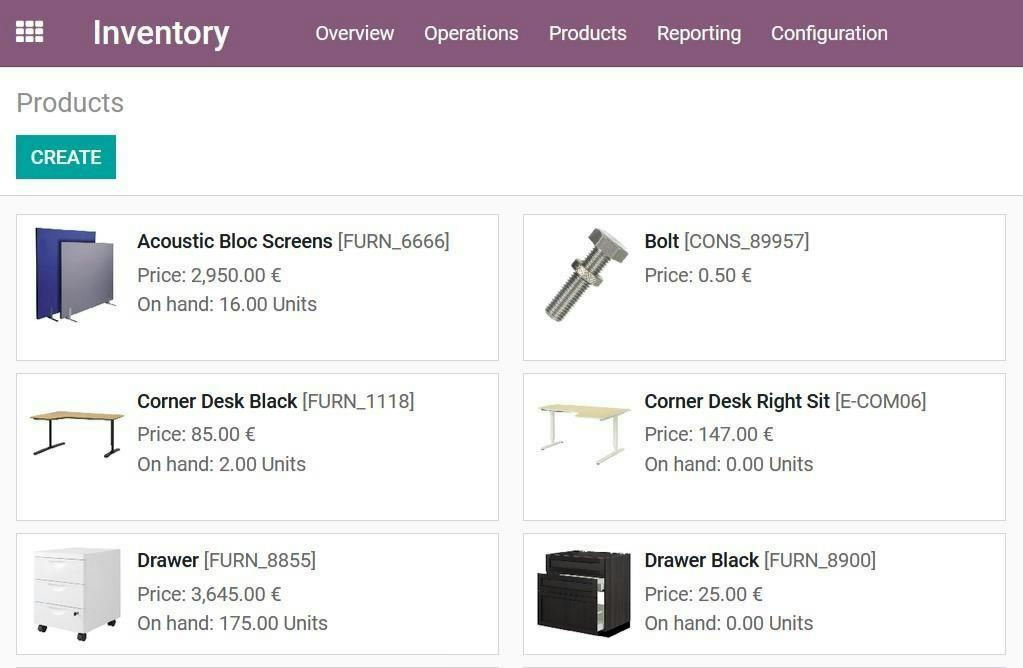
\includegraphics[width=444.96pt,height=290.55pt]{latexImage_8c956101102a7d1ba7b23d715603a997.png}}
\put(69.384,-72.56){\fontsize{12}{1}\usefont{T1}{ptm}{m}{n}\selectfont\color{color_29791}如其責任使用者或製造}
\put(189.492,-72.56){\fontsize{12}{1}\usefont{T1}{ptm}{m}{n}\selectfont\color{color_29791}所需的物料清單。}
\put(285.53,-72.56){\fontsize{12}{1}\usefont{T1}{ptm}{m}{n}\selectfont\color{color_29791}Od}
\put(300.05,-72.56){\fontsize{12}{1}\usefont{T1}{ptm}{m}{n}\selectfont\color{color_29791}o}
\put(305.93,-72.56){\fontsize{12}{1}\usefont{T1}{ptm}{m}{n}\selectfont\color{color_29791}o}
\put(312.07,-72.56){\fontsize{12}{1}\usefont{T1}{ptm}{m}{n}\selectfont\color{color_29791}使所有這些資訊都可以}
\put(432.178,-72.56){\fontsize{12}{1}\usefont{T1}{ptm}{m}{n}\selectfont\color{color_29791}通過其瀏覽器}
\put(69.384,-90.34003){\fontsize{12}{1}\usefont{T1}{ptm}{m}{n}\selectfont\color{color_29791}介}
\put(81.492,-90.34003){\fontsize{12}{1}\usefont{T1}{ptm}{m}{n}\selectfont\color{color_29791}面}
\put(93.60001,-90.34003){\fontsize{12}{1}\usefont{T1}{ptm}{m}{n}\selectfont\color{color_29791}訪}
\put(105.708,-90.34003){\fontsize{12}{1}\usefont{T1}{ptm}{m}{n}\selectfont\color{color_29791}問}
\put(117.816,-90.34003){\fontsize{12}{1}\usefont{T1}{ptm}{m}{n}\selectfont\color{color_29791}和交}
\put(141.924,-90.34003){\fontsize{12}{1}\usefont{T1}{ptm}{m}{n}\selectfont\color{color_29791}互}
\put(154.032,-90.34003){\fontsize{12}{1}\usefont{T1}{ptm}{m}{n}\selectfont\color{color_29791}(}
\put(166.14,-90.34003){\fontsize{12}{1}\usefont{T1}{ptm}{m}{n}\selectfont\color{color_29791}圖}
\put(178.34,-90.34003){\fontsize{12}{1}\usefont{T1}{ptm}{m}{n}\selectfont\color{color_29791}19}
\put(190.25,-90.34003){\fontsize{12}{1}\usefont{T1}{ptm}{m}{n}\selectfont\color{color_29791}和圖}
\put(214.49,-90.34003){\fontsize{12}{1}\usefont{T1}{ptm}{m}{n}\selectfont\color{color_29791}20}
\put(226.49,-90.34003){\fontsize{12}{1}\usefont{T1}{ptm}{m}{n}\selectfont\color{color_29791})}
\put(238.598,-90.34003){\fontsize{12}{1}\usefont{T1}{ptm}{m}{n}\selectfont\color{color_29791}。}
\put(250.706,-90.34003){\fontsize{12}{1}\usefont{T1}{ptm}{m}{n}\selectfont\color{color_29791}為了}
\put(274.814,-90.34003){\fontsize{12}{1}\usefont{T1}{ptm}{m}{n}\selectfont\color{color_29791}保}
\put(286.922,-90.34003){\fontsize{12}{1}\usefont{T1}{ptm}{m}{n}\selectfont\color{color_29791}持}
\put(299.03,-90.34003){\fontsize{12}{1}\usefont{T1}{ptm}{m}{n}\selectfont\color{color_29791}一致}
\put(323.138,-90.34003){\fontsize{12}{1}\usefont{T1}{ptm}{m}{n}\selectfont\color{color_29791}性}
\put(335.246,-90.34003){\fontsize{12}{1}\usefont{T1}{ptm}{m}{n}\selectfont\color{color_29791},}
\put(347.354,-90.34003){\fontsize{12}{1}\usefont{T1}{ptm}{m}{n}\selectfont\color{color_29791}本}
\put(359.462,-90.34003){\fontsize{12}{1}\usefont{T1}{ptm}{m}{n}\selectfont\color{color_29791}文檔}
\put(383.57,-90.34003){\fontsize{12}{1}\usefont{T1}{ptm}{m}{n}\selectfont\color{color_29791}將}
\put(395.678,-90.34003){\fontsize{12}{1}\usefont{T1}{ptm}{m}{n}\selectfont\color{color_29791}特}
\put(407.786,-90.34003){\fontsize{12}{1}\usefont{T1}{ptm}{m}{n}\selectfont\color{color_29791}定專案}
\put(443.894,-90.34003){\fontsize{12}{1}\usefont{T1}{ptm}{m}{n}\selectfont\color{color_29791}表}
\put(456.002,-90.34003){\fontsize{12}{1}\usefont{T1}{ptm}{m}{n}\selectfont\color{color_29791}示}
\put(468.11,-90.34003){\fontsize{12}{1}\usefont{T1}{ptm}{m}{n}\selectfont\color{color_29791}(}
\put(480.218,-90.34003){\fontsize{12}{1}\usefont{T1}{ptm}{m}{n}\selectfont\color{color_29791}例如}
\put(504.22,-90.34003){\fontsize{12}{1}\usefont{T1}{ptm}{m}{n}\selectfont\color{color_29791} }
\put(69.384,-108.34){\fontsize{12}{1}\usefont{T1}{ptm}{m}{n}\selectfont\color{color_29791}B}
\put(77.304,-108.34){\fontsize{12}{1}\usefont{T1}{ptm}{m}{n}\selectfont\color{color_29791}o}
\put(83.184,-108.34){\fontsize{12}{1}\usefont{T1}{ptm}{m}{n}\selectfont\color{color_29791}l}
\put(86.424,-108.34){\fontsize{12}{1}\usefont{T1}{ptm}{m}{n}\selectfont\color{color_29791}t}
\put(89.66,-108.34){\fontsize{12}{1}\usefont{T1}{ptm}{m}{n}\selectfont\color{color_29791})稱為}
\put(125.3,-108.34){\fontsize{12}{1}\usefont{T1}{ptm}{m}{n}\selectfont\color{color_29791}“}
\put(130.46,-108.34){\fontsize{12}{1}\usefont{T1}{ptm}{m}{n}\selectfont\color{color_29791}專案}
\put(154.34,-108.34){\fontsize{12}{1}\usefont{T1}{ptm}{m}{n}\selectfont\color{color_29791}”}
\put(159.5,-108.34){\fontsize{12}{1}\usefont{T1}{ptm}{m}{n}\selectfont\color{color_29791},}
\put(171.38,-108.34){\fontsize{12}{1}\usefont{T1}{ptm}{m}{n}\selectfont\color{color_29791}並將}
\put(195.26,-108.34){\fontsize{12}{1}\usefont{T1}{ptm}{m}{n}\selectfont\color{color_29791}專}
\put(207.14,-108.34){\fontsize{12}{1}\usefont{T1}{ptm}{m}{n}\selectfont\color{color_29791}案}
\put(219.02,-108.34){\fontsize{12}{1}\usefont{T1}{ptm}{m}{n}\selectfont\color{color_29791}類}
\put(230.9,-108.34){\fontsize{12}{1}\usefont{T1}{ptm}{m}{n}\selectfont\color{color_29791}型}
\put(242.78,-108.34){\fontsize{12}{1}\usefont{T1}{ptm}{m}{n}\selectfont\color{color_29791}(}
\put(254.66,-108.34){\fontsize{12}{1}\usefont{T1}{ptm}{m}{n}\selectfont\color{color_29791}產}
\put(266.54,-108.34){\fontsize{12}{1}\usefont{T1}{ptm}{m}{n}\selectfont\color{color_29791}品)}
\put(290.42,-108.34){\fontsize{12}{1}\usefont{T1}{ptm}{m}{n}\selectfont\color{color_29791}稱為}
\put(314.35,-108.34){\fontsize{12}{1}\usefont{T1}{ptm}{m}{n}\selectfont\color{color_29791}“}
\put(319.51,-108.34){\fontsize{12}{1}\usefont{T1}{ptm}{m}{n}\selectfont\color{color_29791}專案類}
\put(355.27,-108.34){\fontsize{12}{1}\usefont{T1}{ptm}{m}{n}\selectfont\color{color_29791}”}
\put(360.43,-108.34){\fontsize{12}{1}\usefont{T1}{ptm}{m}{n}\selectfont\color{color_29791}。}
\put(372.43,-108.34){\fontsize{12}{1}\usefont{T1}{ptm}{m}{n}\selectfont\color{color_29791} }
\put(63.024,-125.62){\fontsize{9.96}{1}\usefont{T1}{ptm}{m}{n}\selectfont\color{color_29791} }
\put(210.05,-440.07){\fontsize{12}{1}\usefont{T1}{ptm}{b}{n}\selectfont\color{color_29791}圖}
\put(222.05,-440.07){\fontsize{12}{1}\usefont{T1}{ptm}{b}{n}\selectfont\color{color_29791}19}
\put(234.05,-440.07){\fontsize{12}{1}\usefont{T1}{ptm}{b}{n}\selectfont\color{color_29791} }
\put(237.05,-440.07){\fontsize{12}{1}\usefont{T1}{ptm}{b}{n}\selectfont\color{color_29791}Od}
\put(253.118,-440.07){\fontsize{12}{1}\usefont{T1}{ptm}{b}{n}\selectfont\color{color_29791}oo}
\put(265.13,-440.07){\fontsize{12}{1}\usefont{T1}{ptm}{b}{n}\selectfont\color{color_29791}關於專案的介面示例}
\put(372.19,-440.07){\fontsize{12}{1}\usefont{T1}{ptm}{b}{n}\selectfont\color{color_29791} }
\end{picture}
\newpage
\begin{tikzpicture}[overlay]\path(0pt,0pt);\end{tikzpicture}
\begin{picture}(-5,0)(2.5,0)
\put(500.26,-727.616){\fontsize{12}{1}\usefont{T1}{ptm}{m}{n}\selectfont\color{color_29791}29}
\put(511.78,-727.616){\fontsize{12}{1}\usefont{T1}{ptm}{m}{n}\selectfont\color{color_29791} }
\put(63.024,-726.896){\fontsize{9.96}{1}\usefont{T1}{ptm}{m}{n}\selectfont\color{color_29791} }
\put(507.58,-338.77){\fontsize{9.96}{1}\usefont{T1}{ptm}{m}{n}\selectfont\color{color_29791} }
\put(182.45,-356.65){\fontsize{12}{1}\usefont{T1}{ptm}{b}{n}\selectfont\color{color_29791}圖}
\put(194.45,-356.65){\fontsize{12}{1}\usefont{T1}{ptm}{b}{n}\selectfont\color{color_29791}20}
\put(206.45,-356.65){\fontsize{12}{1}\usefont{T1}{ptm}{b}{n}\selectfont\color{color_29791} }
\put(209.57,-356.65){\fontsize{12}{1}\usefont{T1}{ptm}{b}{n}\selectfont\color{color_29791}GUI}
\put(232.25,-356.65){\fontsize{12}{1}\usefont{T1}{ptm}{b}{n}\selectfont\color{color_29791}顯示的}
\put(268.13,-356.65){\fontsize{12}{1}\usefont{T1}{ptm}{b}{n}\selectfont\color{color_29791}特定}
\put(292.01,-356.65){\fontsize{12}{1}\usefont{T1}{ptm}{b}{n}\selectfont\color{color_29791}專}
\put(303.89,-356.65){\fontsize{12}{1}\usefont{T1}{ptm}{b}{n}\selectfont\color{color_29791}案及其}
\put(339.77,-356.65){\fontsize{12}{1}\usefont{T1}{ptm}{b}{n}\selectfont\color{color_29791}元數據}
\put(375.65,-356.65){\fontsize{12}{1}\usefont{T1}{ptm}{b}{n}\selectfont\color{color_29791}示例}
\put(399.55,-356.65){\fontsize{12}{1}\usefont{T1}{ptm}{b}{n}\selectfont\color{color_29791} }
\put(69.384,-383.89){\fontsize{12}{1}\usefont{T1}{ptm}{m}{n}\selectfont\color{color_29791}在}
\put(81.384,-383.89){\fontsize{12}{1}\usefont{T1}{ptm}{m}{n}\selectfont\color{color_29791}Odo}
\put(102.02,-383.89){\fontsize{12}{1}\usefont{T1}{ptm}{m}{n}\selectfont\color{color_29791}o}
\put(108.02,-383.89){\fontsize{12}{1}\usefont{T1}{ptm}{m}{n}\selectfont\color{color_29791}中,有幾種類型的專案類(有些包含大量元數據,有些保存很少),它們都}
\put(69.384,-401.77){\fontsize{12}{1}\usefont{T1}{ptm}{m}{n}\selectfont\color{color_29791}具有不同程度的關係和集成。由於這項工作的範圍僅限於}
\put(369.43,-401.77){\fontsize{12}{1}\usefont{T1}{ptm}{m}{n}\selectfont\color{color_29791} }
\put(396.67,-401.77){\fontsize{12}{1}\usefont{T1}{ptm}{m}{n}\selectfont\color{color_29791}P}
\put(403.51,-401.77){\fontsize{12}{1}\usefont{T1}{ptm}{m}{n}\selectfont\color{color_29791}L}
\put(410.59,-401.77){\fontsize{12}{1}\usefont{T1}{ptm}{m}{n}\selectfont\color{color_29791}M}
\put(421.27,-401.77){\fontsize{12}{1}\usefont{T1}{ptm}{m}{n}\selectfont\color{color_29791} }
\put(448.78,-401.77){\fontsize{12}{1}\usefont{T1}{ptm}{m}{n}\selectfont\color{color_29791}和}
\put(460.78,-401.77){\fontsize{12}{1}\usefont{T1}{ptm}{m}{n}\selectfont\color{color_29791} }
\put(487.9,-401.77){\fontsize{12}{1}\usefont{T1}{ptm}{m}{n}\selectfont\color{color_29791}M}
\put(498.22,-401.77){\fontsize{12}{1}\usefont{T1}{ptm}{m}{n}\selectfont\color{color_29791}E}
\put(505.18,-401.77){\fontsize{12}{1}\usefont{T1}{ptm}{m}{n}\selectfont\color{color_29791}S}
\put(69.384,-419.67){\fontsize{12}{1}\usefont{T1}{ptm}{m}{n}\selectfont\color{color_29791}功}
\put(81.384,-419.67){\fontsize{12}{1}\usefont{T1}{ptm}{m}{n}\selectfont\color{color_29791}能}
\put(93.38,-419.67){\fontsize{12}{1}\usefont{T1}{ptm}{m}{n}\selectfont\color{color_29791},因此重點放在與之相關的專案上。以下各節將對}
\put(357.43,-419.67){\fontsize{12}{1}\usefont{T1}{ptm}{m}{n}\selectfont\color{color_29791}Odo}
\put(378.07,-419.67){\fontsize{12}{1}\usefont{T1}{ptm}{m}{n}\selectfont\color{color_29791}o}
\put(384.07,-419.67){\fontsize{12}{1}\usefont{T1}{ptm}{m}{n}\selectfont\color{color_29791}製造過程的主要}
\put(468.1,-419.67){\fontsize{12}{1}\usefont{T1}{ptm}{m}{n}\selectfont\color{color_29791}7}
\put(474.1,-419.67){\fontsize{12}{1}\usefont{T1}{ptm}{m}{n}\selectfont\color{color_29791}個專案}
\put(69.384,-437.55){\fontsize{12}{1}\usefont{T1}{ptm}{m}{n}\selectfont\color{color_29791}類別進行簡短的解}
\put(165.38,-437.55){\fontsize{12}{1}\usefont{T1}{ptm}{m}{n}\selectfont\color{color_29791}釋}
\put(177.38,-437.55){\fontsize{12}{1}\usefont{T1}{ptm}{m}{n}\selectfont\color{color_29791},因為它的基本理解有助於讀者遵循類比。如下圖所示(圖}
\put(489.46,-437.55){\fontsize{12}{1}\usefont{T1}{ptm}{m}{n}\selectfont\color{color_29791} }
\put(69.384,-455.43){\fontsize{12}{1}\usefont{T1}{ptm}{m}{n}\selectfont\color{color_29791}21}
\put(81.384,-455.43){\fontsize{12}{1}\usefont{T1}{ptm}{m}{n}\selectfont\color{color_29791})}
\put(93.38,-455.43){\fontsize{12}{1}\usefont{T1}{ptm}{m}{n}\selectfont\color{color_29791}。}
\put(105.38,-455.43){\fontsize{12}{1}\usefont{T1}{ptm}{m}{n}\selectfont\color{color_29791}製造過程外部的其他專案將在整個模擬過程中呈}
\put(357.43,-455.43){\fontsize{12}{1}\usefont{T1}{ptm}{m}{n}\selectfont\color{color_29791}現}
\put(369.43,-455.43){\fontsize{12}{1}\usefont{T1}{ptm}{m}{n}\selectfont\color{color_29791}。}
\put(381.43,-455.43){\fontsize{12}{1}\usefont{T1}{ptm}{m}{n}\selectfont\color{color_29791} }
\put(73.75,-338.7){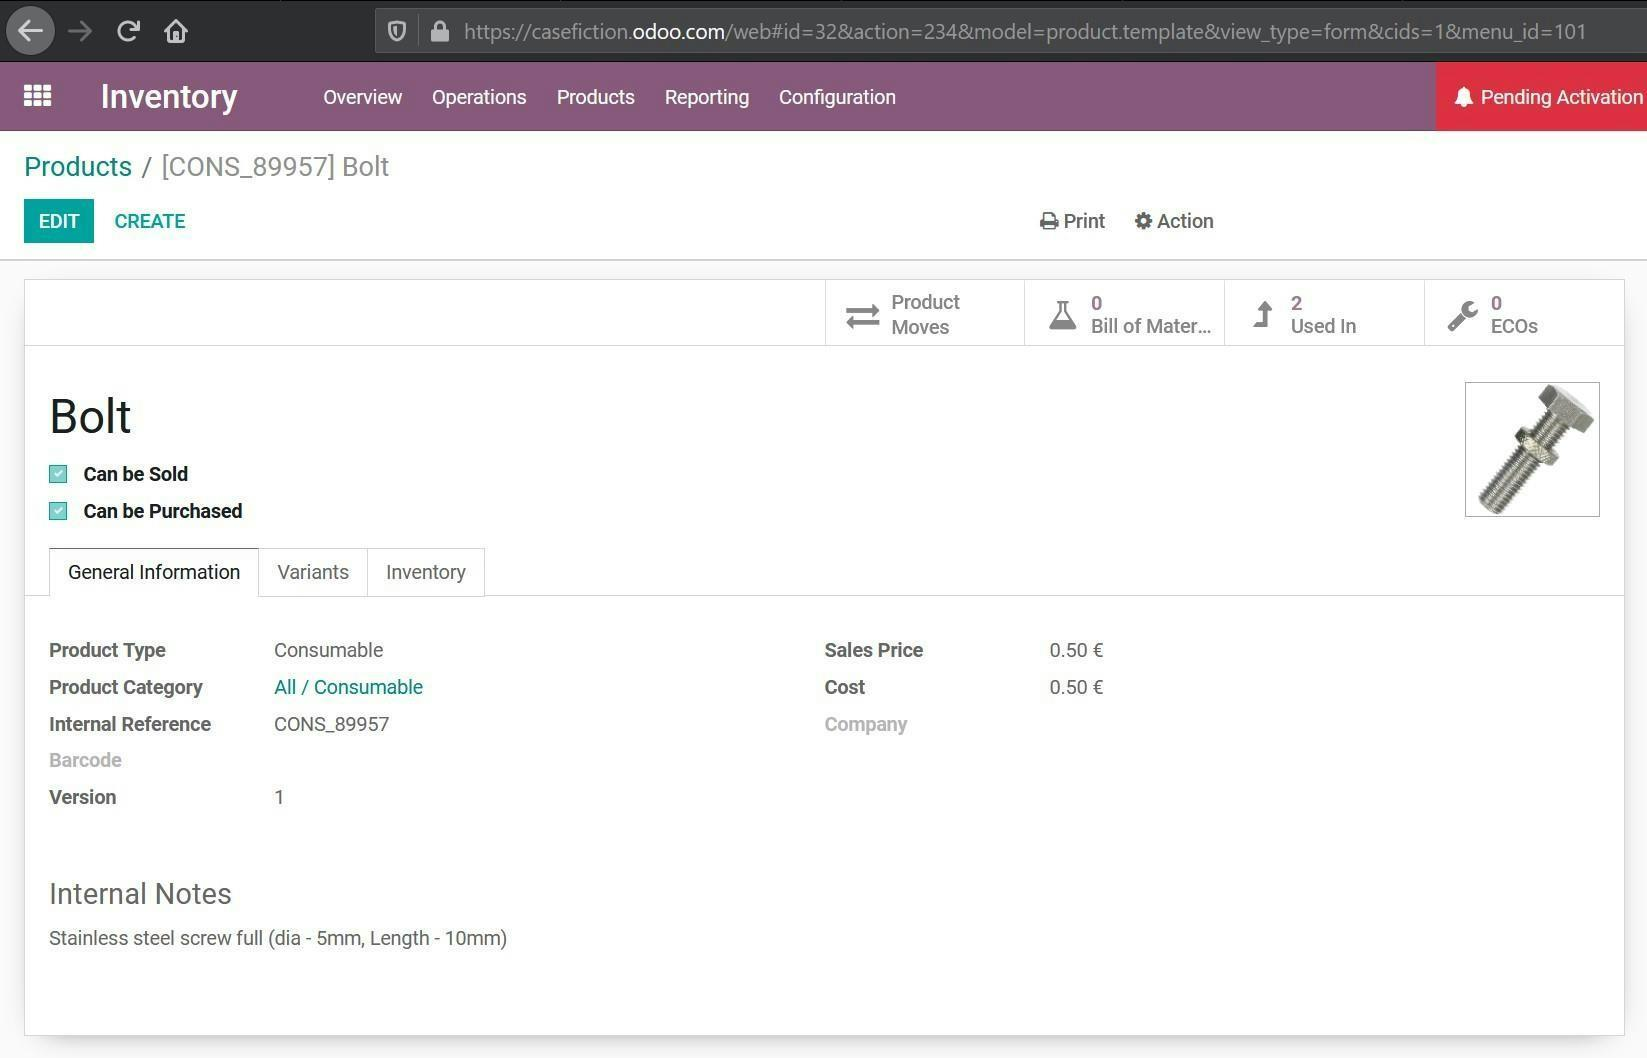
\includegraphics[width=433.7pt,height=277.7pt]{latexImage_4b962cffcbf2429ed5ae48628a4eb939.png}}
\end{picture}
\newpage
\begin{tikzpicture}[overlay]\path(0pt,0pt);\end{tikzpicture}
\begin{picture}(-5,0)(2.5,0)
\put(500.26,-727.616){\fontsize{12}{1}\usefont{T1}{ptm}{m}{n}\selectfont\color{color_29791}30}
\put(511.78,-727.616){\fontsize{12}{1}\usefont{T1}{ptm}{m}{n}\selectfont\color{color_29791} }
\put(63.024,-726.896){\fontsize{9.96}{1}\usefont{T1}{ptm}{m}{n}\selectfont\color{color_29791} }
\put(528.22,-530.79){\fontsize{9.96}{1}\usefont{T1}{ptm}{m}{n}\selectfont\color{color_29791} }
\put(86.06,-556.71){\fontsize{12}{1}\usefont{T1}{ptm}{b}{n}\selectfont\color{color_29791}圖}
\put(98.06,-556.71){\fontsize{12}{1}\usefont{T1}{ptm}{b}{n}\selectfont\color{color_29791} }
\put(101.06,-556.71){\fontsize{12}{1}\usefont{T1}{ptm}{b}{n}\selectfont\color{color_29791}21}
\put(113.06,-556.71){\fontsize{12}{1}\usefont{T1}{ptm}{b}{n}\selectfont\color{color_29791} }
\put(115.94,-556.71){\fontsize{12}{1}\usefont{T1}{ptm}{b}{n}\selectfont\color{color_29791}簡化物料與產品}
\put(200.048,-556.71){\fontsize{12}{1}\usefont{T1}{ptm}{b}{n}\selectfont\color{color_29791}製造的關係圖}
\put(272.09,-556.71){\fontsize{12}{1}\usefont{T1}{ptm}{b}{n}\selectfont\color{color_29791} }
\put(275.09,-556.71){\fontsize{12}{1}\usefont{T1}{ptm}{b}{n}\selectfont\color{color_29791}X}
\put(283.25,-556.71){\fontsize{12}{1}\usefont{T1}{ptm}{b}{n}\selectfont\color{color_29791} }
\put(63.024,-573.27){\fontsize{12}{1}\usefont{T1}{ptm}{b}{n}\selectfont\color{color_29791} }
\put(63.024,-591.3){\fontsize{12}{1}\usefont{T1}{ptm}{b}{n}\selectfont\color{color_29791} }
\put(124.1,-609.3){\fontsize{12}{1}\usefont{T1}{ptm}{b}{n}\selectfont\color{color_29791}5.1.3.1.}
\put(160.1,-609.3){\fontsize{12}{1}\usefont{T1}{ptm}{b}{n}\selectfont\color{color_29791} }
\put(188.21,-609.3){\fontsize{12}{1}\usefont{T1}{ptm}{b}{n}\selectfont\color{color_29791}產品專案}
\put(235.61,-609.3){\fontsize{12}{1}\usefont{T1}{ptm}{b}{n}\selectfont\color{color_29791} }
\put(82.944,-638.82){\fontsize{12}{1}\usefont{T1}{ptm}{m}{n}\selectfont\color{color_29791}每種材料、元件或}
\put(178.092,-638.82){\fontsize{12}{1}\usefont{T1}{ptm}{m}{n}\selectfont\color{color_29791}產品}
\put(201.96,-638.82){\fontsize{12}{1}\usefont{T1}{ptm}{m}{n}\selectfont\color{color_29791}都以產品類型類為}
\put(297.108,-638.82){\fontsize{12}{1}\usefont{T1}{ptm}{m}{n}\selectfont\color{color_29791}特徵}
\put(320.976,-638.82){\fontsize{12}{1}\usefont{T1}{ptm}{m}{n}\selectfont\color{color_29791},該類主要在}
\put(392.35,-638.82){\fontsize{12}{1}\usefont{T1}{ptm}{m}{n}\selectfont\color{color_29791}Od}
\put(406.87,-638.82){\fontsize{12}{1}\usefont{T1}{ptm}{m}{n}\selectfont\color{color_29791}o}
\put(412.75,-638.82){\fontsize{12}{1}\usefont{T1}{ptm}{m}{n}\selectfont\color{color_29791}o}
\put(418.63,-638.82){\fontsize{12}{1}\usefont{T1}{ptm}{m}{n}\selectfont\color{color_29791}的}
\put(430.51,-638.82){\fontsize{12}{1}\usefont{T1}{ptm}{m}{n}\selectfont\color{color_29791}庫存}
\put(454.39,-638.82){\fontsize{12}{1}\usefont{T1}{ptm}{m}{n}\selectfont\color{color_29791}應}
\put(466.27,-638.82){\fontsize{12}{1}\usefont{T1}{ptm}{m}{n}\selectfont\color{color_29791}用}
\put(478.15,-638.82){\fontsize{12}{1}\usefont{T1}{ptm}{m}{n}\selectfont\color{color_29791}程}
\put(490.03,-638.82){\fontsize{12}{1}\usefont{T1}{ptm}{m}{n}\selectfont\color{color_29791}式}
\put(69.384,-656.58){\fontsize{12}{1}\usefont{T1}{ptm}{m}{n}\selectfont\color{color_29791}中保存和管理。這}
\put(164.532,-656.58){\fontsize{12}{1}\usefont{T1}{ptm}{m}{n}\selectfont\color{color_29791}意味}
\put(188.4,-656.58){\fontsize{12}{1}\usefont{T1}{ptm}{m}{n}\selectfont\color{color_29791}著,在系統內,產}
\put(283.548,-656.58){\fontsize{12}{1}\usefont{T1}{ptm}{m}{n}\selectfont\color{color_29791}品生}
\put(307.416,-656.58){\fontsize{12}{1}\usefont{T1}{ptm}{m}{n}\selectfont\color{color_29791}產取決於其他產品}
\put(402.564,-656.58){\fontsize{12}{1}\usefont{T1}{ptm}{m}{n}\selectfont\color{color_29791}的可}
\put(426.432,-656.58){\fontsize{12}{1}\usefont{T1}{ptm}{m}{n}\selectfont\color{color_29791}用性,這些產}
\put(69.384,-674.34){\fontsize{12}{1}\usefont{T1}{ptm}{m}{n}\selectfont\color{color_29791}品要麼按原樣購買}
\put(164.532,-674.34){\fontsize{12}{1}\usefont{T1}{ptm}{m}{n}\selectfont\color{color_29791},要}
\put(188.4,-674.34){\fontsize{12}{1}\usefont{T1}{ptm}{m}{n}\selectfont\color{color_29791}麼從其他產品製造}
\put(283.548,-674.34){\fontsize{12}{1}\usefont{T1}{ptm}{m}{n}\selectfont\color{color_29791}(圖}
\put(307.49,-674.34){\fontsize{12}{1}\usefont{T1}{ptm}{m}{n}\selectfont\color{color_29791}22}
\put(319.27,-674.34){\fontsize{12}{1}\usefont{T1}{ptm}{m}{n}\selectfont\color{color_29791})}
\put(331.15,-674.34){\fontsize{12}{1}\usefont{T1}{ptm}{m}{n}\selectfont\color{color_29791},}
\put(343.03,-674.34){\fontsize{12}{1}\usefont{T1}{ptm}{m}{n}\selectfont\color{color_29791}即}
\put(354.91,-674.34){\fontsize{12}{1}\usefont{T1}{ptm}{m}{n}\selectfont\color{color_29791}原}
\put(366.79,-674.34){\fontsize{12}{1}\usefont{T1}{ptm}{m}{n}\selectfont\color{color_29791}材}
\put(378.67,-674.34){\fontsize{12}{1}\usefont{T1}{ptm}{m}{n}\selectfont\color{color_29791}料也}
\put(402.55,-674.34){\fontsize{12}{1}\usefont{T1}{ptm}{m}{n}\selectfont\color{color_29791}被}
\put(414.43,-674.34){\fontsize{12}{1}\usefont{T1}{ptm}{m}{n}\selectfont\color{color_29791}視為}
\put(438.31,-674.34){\fontsize{12}{1}\usefont{T1}{ptm}{m}{n}\selectfont\color{color_29791}產}
\put(450.19,-674.34){\fontsize{12}{1}\usefont{T1}{ptm}{m}{n}\selectfont\color{color_29791}品}
\put(462.07,-674.34){\fontsize{12}{1}\usefont{T1}{ptm}{m}{n}\selectfont\color{color_29791},}
\put(473.95,-674.34){\fontsize{12}{1}\usefont{T1}{ptm}{m}{n}\selectfont\color{color_29791}更}
\put(485.83,-674.34){\fontsize{12}{1}\usefont{T1}{ptm}{m}{n}\selectfont\color{color_29791}具}
\put(497.86,-674.34){\fontsize{12}{1}\usefont{T1}{ptm}{m}{n}\selectfont\color{color_29791} }
\put(87.9,-530.75){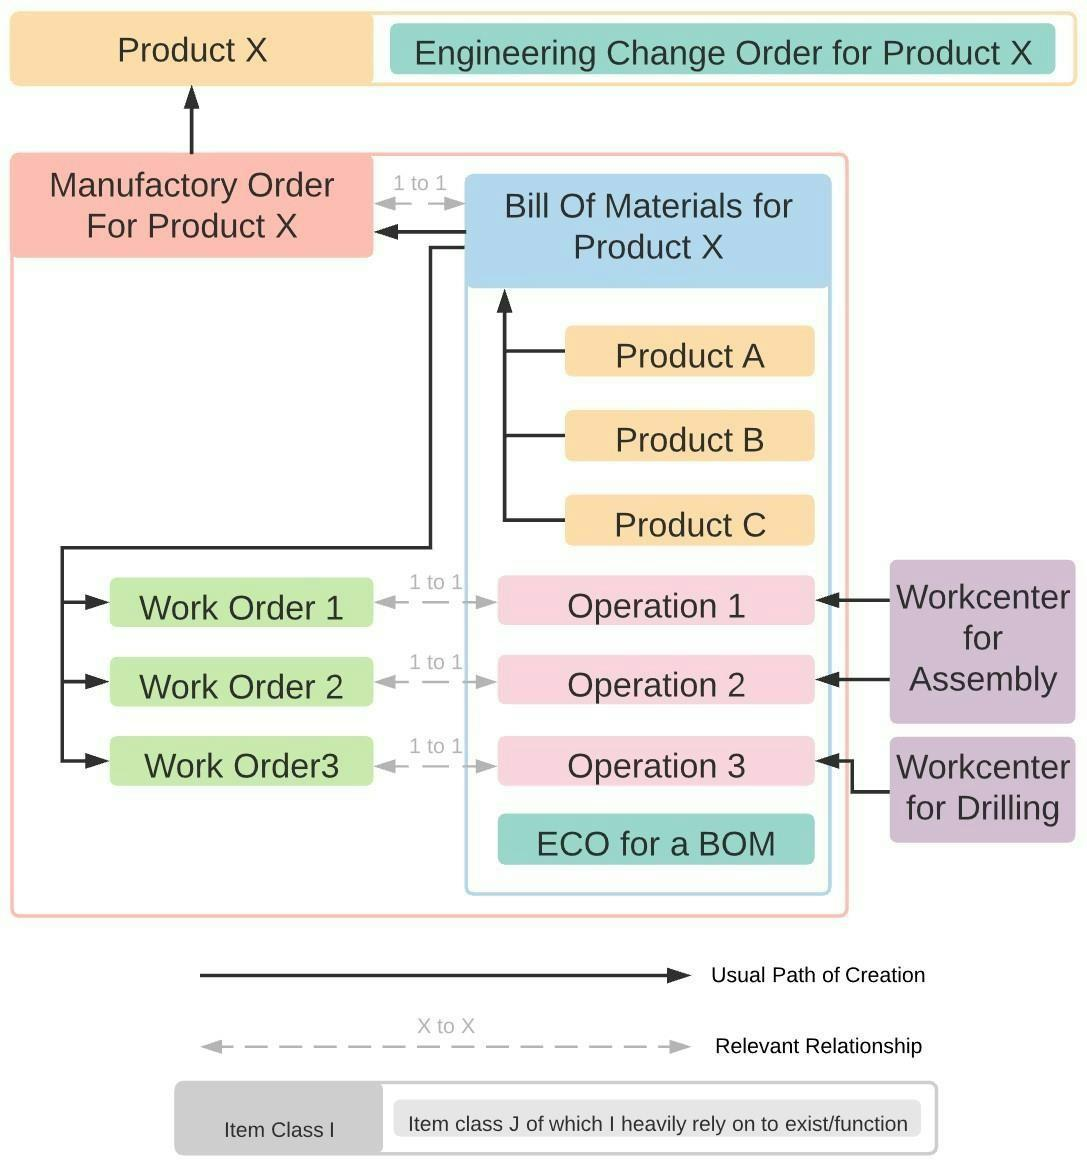
\includegraphics[width=440.29pt,height=469.75pt]{latexImage_31265cf931e1dca057025e727f436f04.png}}
\end{picture}
\newpage
\begin{tikzpicture}[overlay]\path(0pt,0pt);\end{tikzpicture}
\begin{picture}(-5,0)(2.5,0)
\put(500.26,-727.616){\fontsize{12}{1}\usefont{T1}{ptm}{m}{n}\selectfont\color{color_29791}31}
\put(511.78,-727.616){\fontsize{12}{1}\usefont{T1}{ptm}{m}{n}\selectfont\color{color_29791} }
\put(63.024,-726.896){\fontsize{9.96}{1}\usefont{T1}{ptm}{m}{n}\selectfont\color{color_29791} }
\put(137.45,-215.05){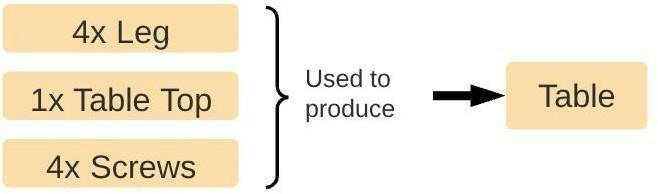
\includegraphics[width=325.6pt,height=95.99999pt]{latexImage_a1b74bb4df4fa0ab5aa003265b46b3e2.png}}
\put(81.55,-494.7){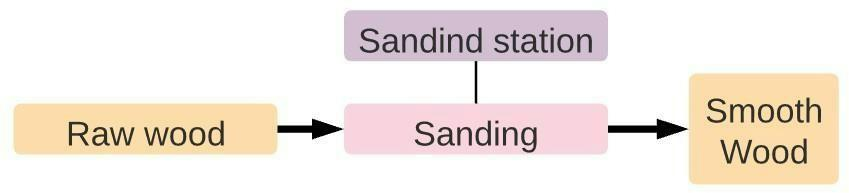
\includegraphics[width=413.78pt,height=94.05pt]{latexImage_d04d11d213a61554b2a4b18956747a5a.png}}
\put(69.384,-72.56){\fontsize{12}{1}\usefont{T1}{ptm}{m}{n}\selectfont\color{color_29791}體地說,是購買的}
\put(164.532,-72.56){\fontsize{12}{1}\usefont{T1}{ptm}{m}{n}\selectfont\color{color_29791}產品}
\put(188.4,-72.56){\fontsize{12}{1}\usefont{T1}{ptm}{m}{n}\selectfont\color{color_29791},然後包含在}
\put(259.73,-72.56){\fontsize{12}{1}\usefont{T1}{ptm}{m}{n}\selectfont\color{color_29791}B}
\put(267.65,-72.56){\fontsize{12}{1}\usefont{T1}{ptm}{m}{n}\selectfont\color{color_29791}O}
\put(276.17,-72.56){\fontsize{12}{1}\usefont{T1}{ptm}{m}{n}\selectfont\color{color_29791}M}
\put(286.85,-72.56){\fontsize{12}{1}\usefont{T1}{ptm}{m}{n}\selectfont\color{color_29791}中}
\put(298.73,-72.56){\fontsize{12}{1}\usefont{T1}{ptm}{m}{n}\selectfont\color{color_29791}以製}
\put(322.61,-72.56){\fontsize{12}{1}\usefont{T1}{ptm}{m}{n}\selectfont\color{color_29791}造}
\put(334.49,-72.56){\fontsize{12}{1}\usefont{T1}{ptm}{m}{n}\selectfont\color{color_29791}其}
\put(346.37,-72.56){\fontsize{12}{1}\usefont{T1}{ptm}{m}{n}\selectfont\color{color_29791}他}
\put(358.25,-72.56){\fontsize{12}{1}\usefont{T1}{ptm}{m}{n}\selectfont\color{color_29791}產}
\put(370.13,-72.56){\fontsize{12}{1}\usefont{T1}{ptm}{m}{n}\selectfont\color{color_29791}品}
\put(382.01,-72.56){\fontsize{12}{1}\usefont{T1}{ptm}{m}{n}\selectfont\color{color_29791}。}
\put(393.89,-72.56){\fontsize{12}{1}\usefont{T1}{ptm}{m}{n}\selectfont\color{color_29791}這被}
\put(417.7701,-72.56){\fontsize{12}{1}\usefont{T1}{ptm}{m}{n}\selectfont\color{color_29791}認為}
\put(441.6501,-72.56){\fontsize{12}{1}\usefont{T1}{ptm}{m}{n}\selectfont\color{color_29791}是}
\put(453.5301,-72.56){\fontsize{12}{1}\usefont{T1}{ptm}{m}{n}\selectfont\color{color_29791}主}
\put(465.4101,-72.56){\fontsize{12}{1}\usefont{T1}{ptm}{m}{n}\selectfont\color{color_29791}要}
\put(477.2901,-72.56){\fontsize{12}{1}\usefont{T1}{ptm}{m}{n}\selectfont\color{color_29791}專}
\put(489.1701,-72.56){\fontsize{12}{1}\usefont{T1}{ptm}{m}{n}\selectfont\color{color_29791}案}
\put(69.384,-90.46002){\fontsize{12}{1}\usefont{T1}{ptm}{m}{n}\selectfont\color{color_29791}類,因為它既是製}
\put(164.532,-90.46002){\fontsize{12}{1}\usefont{T1}{ptm}{m}{n}\selectfont\color{color_29791}造的}
\put(188.4,-90.46002){\fontsize{12}{1}\usefont{T1}{ptm}{m}{n}\selectfont\color{color_29791}來源,也是製造的}
\put(283.548,-90.46002){\fontsize{12}{1}\usefont{T1}{ptm}{m}{n}\selectfont\color{color_29791}目標}
\put(307.416,-90.46002){\fontsize{12}{1}\usefont{T1}{ptm}{m}{n}\selectfont\color{color_29791}。}
\put(319.39,-90.46002){\fontsize{12}{1}\usefont{T1}{ptm}{m}{n}\selectfont\color{color_29791} }
\put(63.024,-115.18){\fontsize{9.96}{1}\usefont{T1}{ptm}{m}{n}\selectfont\color{color_29791} }
\put(237.29,-233.5){\fontsize{12}{1}\usefont{T1}{ptm}{b}{n}\selectfont\color{color_29791}圖}
\put(249.29,-233.5){\fontsize{12}{1}\usefont{T1}{ptm}{b}{n}\selectfont\color{color_29791}22}
\put(261.29,-233.5){\fontsize{12}{1}\usefont{T1}{ptm}{b}{n}\selectfont\color{color_29791}簡化產品關係圖}
\put(344.59,-233.5){\fontsize{12}{1}\usefont{T1}{ptm}{b}{n}\selectfont\color{color_29791} }
\put(124.1,-270.73){\fontsize{12}{1}\usefont{T1}{ptm}{b}{n}\selectfont\color{color_29791}5.1.3.2.}
\put(160.1,-270.73){\fontsize{12}{1}\usefont{T1}{ptm}{b}{n}\selectfont\color{color_29791} }
\put(220.97,-270.73){\fontsize{12}{1}\usefont{T1}{ptm}{b}{n}\selectfont\color{color_29791}工序物}
\put(256.85,-270.73){\fontsize{12}{1}\usefont{T1}{ptm}{b}{n}\selectfont\color{color_29791}料類和}
\put(292.73,-270.73){\fontsize{12}{1}\usefont{T1}{ptm}{b}{n}\selectfont\color{color_29791}工作}
\put(316.61,-270.73){\fontsize{12}{1}\usefont{T1}{ptm}{b}{n}\selectfont\color{color_29791}中心}
\put(340.49,-270.73){\fontsize{12}{1}\usefont{T1}{ptm}{b}{n}\selectfont\color{color_29791}物料類}
\put(376.39,-270.73){\fontsize{12}{1}\usefont{T1}{ptm}{b}{n}\selectfont\color{color_29791} }
\put(82.944,-300.13){\fontsize{12}{1}\usefont{T1}{ptm}{m}{n}\selectfont\color{color_29791}工序專案代表將元}
\put(178.092,-300.13){\fontsize{12}{1}\usefont{T1}{ptm}{m}{n}\selectfont\color{color_29791}件或}
\put(201.96,-300.13){\fontsize{12}{1}\usefont{T1}{ptm}{m}{n}\selectfont\color{color_29791}原材料轉化為產品}
\put(297.108,-300.13){\fontsize{12}{1}\usefont{T1}{ptm}{m}{n}\selectfont\color{color_29791}或新}
\put(320.976,-300.13){\fontsize{12}{1}\usefont{T1}{ptm}{m}{n}\selectfont\color{color_29791}元件所需的製造工}
\put(416.124,-300.13){\fontsize{12}{1}\usefont{T1}{ptm}{m}{n}\selectfont\color{color_29791}序,}
\put(439.992,-300.13){\fontsize{12}{1}\usefont{T1}{ptm}{m}{n}\selectfont\color{color_29791}而工作中心}
\put(69.384,-318.01){\fontsize{12}{1}\usefont{T1}{ptm}{m}{n}\selectfont\color{color_29791}專案則代表工序發}
\put(164.532,-318.01){\fontsize{12}{1}\usefont{T1}{ptm}{m}{n}\selectfont\color{color_29791}生的}
\put(188.4,-318.01){\fontsize{12}{1}\usefont{T1}{ptm}{m}{n}\selectfont\color{color_29791}地方,例如,在具}
\put(283.548,-318.01){\fontsize{12}{1}\usefont{T1}{ptm}{m}{n}\selectfont\color{color_29791}有適}
\put(307.416,-318.01){\fontsize{12}{1}\usefont{T1}{ptm}{m}{n}\selectfont\color{color_29791}當設備的砂光站(}
\put(402.564,-318.01){\fontsize{12}{1}\usefont{T1}{ptm}{m}{n}\selectfont\color{color_29791}圖}
\put(414.67,-318.01){\fontsize{12}{1}\usefont{T1}{ptm}{m}{n}\selectfont\color{color_29791} }
\put(69.384,-335.89){\fontsize{12}{1}\usefont{T1}{ptm}{m}{n}\selectfont\color{color_29791}23}
\put(81.144,-335.89){\fontsize{12}{1}\usefont{T1}{ptm}{m}{n}\selectfont\color{color_29791})}
\put(93.02399,-335.89){\fontsize{12}{1}\usefont{T1}{ptm}{m}{n}\selectfont\color{color_29791}中}
\put(104.904,-335.89){\fontsize{12}{1}\usefont{T1}{ptm}{m}{n}\selectfont\color{color_29791}進}
\put(116.784,-335.89){\fontsize{12}{1}\usefont{T1}{ptm}{m}{n}\selectfont\color{color_29791}行}
\put(128.664,-335.89){\fontsize{12}{1}\usefont{T1}{ptm}{m}{n}\selectfont\color{color_29791}打}
\put(140.544,-335.89){\fontsize{12}{1}\usefont{T1}{ptm}{m}{n}\selectfont\color{color_29791}磨木}
\put(164.424,-335.89){\fontsize{12}{1}\usefont{T1}{ptm}{m}{n}\selectfont\color{color_29791}材}
\put(176.304,-335.89){\fontsize{12}{1}\usefont{T1}{ptm}{m}{n}\selectfont\color{color_29791}。該}
\put(200.184,-335.89){\fontsize{12}{1}\usefont{T1}{ptm}{m}{n}\selectfont\color{color_29791}工}
\put(212.064,-335.89){\fontsize{12}{1}\usefont{T1}{ptm}{m}{n}\selectfont\color{color_29791}作}
\put(223.944,-335.89){\fontsize{12}{1}\usefont{T1}{ptm}{m}{n}\selectfont\color{color_29791}中}
\put(235.824,-335.89){\fontsize{12}{1}\usefont{T1}{ptm}{m}{n}\selectfont\color{color_29791}心}
\put(247.704,-335.89){\fontsize{12}{1}\usefont{T1}{ptm}{m}{n}\selectfont\color{color_29791}最}
\put(259.584,-335.89){\fontsize{12}{1}\usefont{T1}{ptm}{m}{n}\selectfont\color{color_29791}終}
\put(271.4641,-335.89){\fontsize{12}{1}\usefont{T1}{ptm}{m}{n}\selectfont\color{color_29791}在}
\put(283.49,-335.89){\fontsize{12}{1}\usefont{T1}{ptm}{m}{n}\selectfont\color{color_29791}O}
\put(292.01,-335.89){\fontsize{12}{1}\usefont{T1}{ptm}{m}{n}\selectfont\color{color_29791}d}
\put(297.89,-335.89){\fontsize{12}{1}\usefont{T1}{ptm}{m}{n}\selectfont\color{color_29791}o}
\put(303.77,-335.89){\fontsize{12}{1}\usefont{T1}{ptm}{m}{n}\selectfont\color{color_29791}o}
\put(309.79,-335.89){\fontsize{12}{1}\usefont{T1}{ptm}{m}{n}\selectfont\color{color_29791}中用作其生產計劃}
\put(404.938,-335.89){\fontsize{12}{1}\usefont{T1}{ptm}{m}{n}\selectfont\color{color_29791}中的}
\put(428.806,-335.89){\fontsize{12}{1}\usefont{T1}{ptm}{m}{n}\selectfont\color{color_29791}時間}
\put(452.62,-335.89){\fontsize{12}{1}\usefont{T1}{ptm}{m}{n}\selectfont\color{color_29791}/}
\put(455.86,-335.89){\fontsize{12}{1}\usefont{T1}{ptm}{m}{n}\selectfont\color{color_29791}設備管理}
\put(69.384,-353.77){\fontsize{12}{1}\usefont{T1}{ptm}{m}{n}\selectfont\color{color_29791}工具。基本上,當}
\put(164.532,-353.77){\fontsize{12}{1}\usefont{T1}{ptm}{m}{n}\selectfont\color{color_29791}生產}
\put(188.4,-353.77){\fontsize{12}{1}\usefont{T1}{ptm}{m}{n}\selectfont\color{color_29791}中心滿負荷運轉時}
\put(283.548,-353.77){\fontsize{12}{1}\usefont{T1}{ptm}{m}{n}\selectfont\color{color_29791},它}
\put(307.416,-353.77){\fontsize{12}{1}\usefont{T1}{ptm}{m}{n}\selectfont\color{color_29791}會暫停後續流程或}
\put(402.564,-353.77){\fontsize{12}{1}\usefont{T1}{ptm}{m}{n}\selectfont\color{color_29791}將流}
\put(426.432,-353.77){\fontsize{12}{1}\usefont{T1}{ptm}{m}{n}\selectfont\color{color_29791}程重定向到備}
\put(69.384,-371.77){\fontsize{12}{1}\usefont{T1}{ptm}{m}{n}\selectfont\color{color_29791}用工作中心。操作}
\put(164.532,-371.77){\fontsize{12}{1}\usefont{T1}{ptm}{m}{n}\selectfont\color{color_29791}項還}
\put(188.4,-371.77){\fontsize{12}{1}\usefont{T1}{ptm}{m}{n}\selectfont\color{color_29791}負責保存生產過程}
\put(283.548,-371.77){\fontsize{12}{1}\usefont{T1}{ptm}{m}{n}\selectfont\color{color_29791}中查}
\put(307.416,-371.77){\fontsize{12}{1}\usefont{T1}{ptm}{m}{n}\selectfont\color{color_29791}閱的指令檔。}
\put(378.91,-371.77){\fontsize{12}{1}\usefont{T1}{ptm}{m}{n}\selectfont\color{color_29791} }
\put(63.024,-396.73){\fontsize{9.96}{1}\usefont{T1}{ptm}{m}{n}\selectfont\color{color_29791} }
\put(249.29,-525.27){\fontsize{12}{1}\usefont{T1}{ptm}{b}{n}\selectfont\color{color_29791}圖}
\put(261.29,-525.27){\fontsize{12}{1}\usefont{T1}{ptm}{b}{n}\selectfont\color{color_29791}23}
\put(273.29,-525.27){\fontsize{12}{1}\usefont{T1}{ptm}{b}{n}\selectfont\color{color_29791}簡化操作圖}
\put(332.83,-525.27){\fontsize{12}{1}\usefont{T1}{ptm}{b}{n}\selectfont\color{color_29791} }
\put(63.024,-557.91){\fontsize{12}{1}\usefont{T1}{ptm}{b}{n}\selectfont\color{color_29791} }
\put(124.1,-578.7){\fontsize{12}{1}\usefont{T1}{ptm}{b}{n}\selectfont\color{color_29791}5.1.3.3.}
\put(160.1,-578.7){\fontsize{12}{1}\usefont{T1}{ptm}{b}{n}\selectfont\color{color_29791} }
\put(221.57,-578.7){\fontsize{12}{1}\usefont{T1}{ptm}{b}{n}\selectfont\color{color_29791}物料清單項類}
\put(292.97,-578.7){\fontsize{12}{1}\usefont{T1}{ptm}{b}{n}\selectfont\color{color_29791} }
\put(82.944,-608.1){\fontsize{12}{1}\usefont{T1}{ptm}{m}{n}\selectfont\color{color_29791}物料清單是構建產品所需的元件清單。然而,在}
\put(334.99,-608.1){\fontsize{12}{1}\usefont{T1}{ptm}{m}{n}\selectfont\color{color_29791}Odo}
\put(355.63,-608.1){\fontsize{12}{1}\usefont{T1}{ptm}{m}{n}\selectfont\color{color_29791}o}
\put(361.63,-608.1){\fontsize{12}{1}\usefont{T1}{ptm}{m}{n}\selectfont\color{color_29791}中,}
\put(385.63,-608.1){\fontsize{12}{1}\usefont{T1}{ptm}{m}{n}\selectfont\color{color_29791}B}
\put(393.55,-608.1){\fontsize{12}{1}\usefont{T1}{ptm}{m}{n}\selectfont\color{color_29791}OM}
\put(412.87,-608.1){\fontsize{12}{1}\usefont{T1}{ptm}{m}{n}\selectfont\color{color_29791}最}
\put(424.87,-608.1){\fontsize{12}{1}\usefont{T1}{ptm}{m}{n}\selectfont\color{color_29791}好}
\put(436.87,-608.1){\fontsize{12}{1}\usefont{T1}{ptm}{m}{n}\selectfont\color{color_29791}用}
\put(448.9,-608.1){\fontsize{12}{1}\usefont{T1}{ptm}{m}{n}\selectfont\color{color_29791}P}
\put(455.74,-608.1){\fontsize{12}{1}\usefont{T1}{ptm}{m}{n}\selectfont\color{color_29791}L}
\put(462.82,-608.1){\fontsize{12}{1}\usefont{T1}{ptm}{m}{n}\selectfont\color{color_29791}M}
\put(473.5,-608.1){\fontsize{12}{1}\usefont{T1}{ptm}{m}{n}\selectfont\color{color_29791}認為生}
\put(69.384,-625.98){\fontsize{12}{1}\usefont{T1}{ptm}{m}{n}\selectfont\color{color_29791}產過程的虛擬表示來描述。考慮到前面提到的工序物料類,乍一看似乎有悖常理,}
\put(69.384,-643.98){\fontsize{12}{1}\usefont{T1}{ptm}{m}{n}\selectfont\color{color_29791}但實際}
\put(105.38,-643.98){\fontsize{12}{1}\usefont{T1}{ptm}{m}{n}\selectfont\color{color_29791}上}
\put(117.38,-643.98){\fontsize{12}{1}\usefont{T1}{ptm}{m}{n}\selectfont\color{color_29791},由於物料清單是複合物料,它直接指向生產最終產品所需的所有物料類}
\put(69.384,-661.86){\fontsize{12}{1}\usefont{T1}{ptm}{m}{n}\selectfont\color{color_29791}型}
\put(81.384,-661.86){\fontsize{12}{1}\usefont{T1}{ptm}{m}{n}\selectfont\color{color_29791}(}
\put(93.38,-661.86){\fontsize{12}{1}\usefont{T1}{ptm}{m}{n}\selectfont\color{color_29791}圖}
\put(105.38,-661.86){\fontsize{12}{1}\usefont{T1}{ptm}{m}{n}\selectfont\color{color_29791} }
\put(129.14,-661.86){\fontsize{12}{1}\usefont{T1}{ptm}{m}{n}\selectfont\color{color_29791}24}
\put(141.14,-661.86){\fontsize{12}{1}\usefont{T1}{ptm}{m}{n}\selectfont\color{color_29791})。例如,假設要構建一個產品,需要}
\put(345.19,-661.86){\fontsize{12}{1}\usefont{T1}{ptm}{m}{n}\selectfont\color{color_29791} }
\put(368.95,-661.86){\fontsize{12}{1}\usefont{T1}{ptm}{m}{n}\selectfont\color{color_29791}3}
\put(374.95,-661.86){\fontsize{12}{1}\usefont{T1}{ptm}{m}{n}\selectfont\color{color_29791} }
\put(398.71,-661.86){\fontsize{12}{1}\usefont{T1}{ptm}{m}{n}\selectfont\color{color_29791}個不同的部件和}
\put(482.74,-661.86){\fontsize{12}{1}\usefont{T1}{ptm}{m}{n}\selectfont\color{color_29791} }
\put(506.5,-661.86){\fontsize{12}{1}\usefont{T1}{ptm}{m}{n}\selectfont\color{color_29791}4}
\put(69.384,-679.74){\fontsize{12}{1}\usefont{T1}{ptm}{m}{n}\selectfont\color{color_29791}個不同的操}
\put(129.38,-679.74){\fontsize{12}{1}\usefont{T1}{ptm}{m}{n}\selectfont\color{color_29791}作}
\put(141.38,-679.74){\fontsize{12}{1}\usefont{T1}{ptm}{m}{n}\selectfont\color{color_29791};}
\put(144.74,-679.74){\fontsize{12}{1}\usefont{T1}{ptm}{m}{n}\selectfont\color{color_29791}所述產}
\put(180.62,-679.74){\fontsize{12}{1}\usefont{T1}{ptm}{m}{n}\selectfont\color{color_29791}品的}
\put(204.65,-679.74){\fontsize{12}{1}\usefont{T1}{ptm}{m}{n}\selectfont\color{color_29791}B}
\put(212.57,-679.74){\fontsize{12}{1}\usefont{T1}{ptm}{m}{n}\selectfont\color{color_29791}OM}
\put(231.89,-679.74){\fontsize{12}{1}\usefont{T1}{ptm}{m}{n}\selectfont\color{color_29791}將列出所}
\put(279.89,-679.74){\fontsize{12}{1}\usefont{T1}{ptm}{m}{n}\selectfont\color{color_29791}有}
\put(291.89,-679.74){\fontsize{12}{1}\usefont{T1}{ptm}{m}{n}\selectfont\color{color_29791}這些產品,並指定它們的使用順序。}
\put(483.94,-679.74){\fontsize{12}{1}\usefont{T1}{ptm}{m}{n}\selectfont\color{color_29791} }
\end{picture}
\newpage
\begin{tikzpicture}[overlay]\path(0pt,0pt);\end{tikzpicture}
\begin{picture}(-5,0)(2.5,0)
\put(500.26,-727.616){\fontsize{12}{1}\usefont{T1}{ptm}{m}{n}\selectfont\color{color_29791}32}
\put(511.78,-727.616){\fontsize{12}{1}\usefont{T1}{ptm}{m}{n}\selectfont\color{color_29791} }
\put(63.024,-726.896){\fontsize{9.96}{1}\usefont{T1}{ptm}{m}{n}\selectfont\color{color_29791} }
\put(515.5,-429.99){\fontsize{9.96}{1}\usefont{T1}{ptm}{m}{n}\selectfont\color{color_29791} }
\put(235.01,-445.35){\fontsize{12}{1}\usefont{T1}{ptm}{b}{n}\selectfont\color{color_29791}圖}
\put(247.01,-445.35){\fontsize{12}{1}\usefont{T1}{ptm}{b}{n}\selectfont\color{color_29791} }
\put(250.01,-445.35){\fontsize{12}{1}\usefont{T1}{ptm}{b}{n}\selectfont\color{color_29791}24}
\put(262.01,-445.35){\fontsize{12}{1}\usefont{T1}{ptm}{b}{n}\selectfont\color{color_29791} }
\put(264.89,-445.35){\fontsize{12}{1}\usefont{T1}{ptm}{b}{n}\selectfont\color{color_29791}簡化的}
\put(300.89,-445.35){\fontsize{12}{1}\usefont{T1}{ptm}{b}{n}\selectfont\color{color_29791} }
\put(303.89,-445.35){\fontsize{12}{1}\usefont{T1}{ptm}{b}{n}\selectfont\color{color_29791}B}
\put(311.918,-445.35){\fontsize{12}{1}\usefont{T1}{ptm}{b}{n}\selectfont\color{color_29791}OM}
\put(332.59,-445.35){\fontsize{12}{1}\usefont{T1}{ptm}{b}{n}\selectfont\color{color_29791} }
\put(335.47,-445.35){\fontsize{12}{1}\usefont{T1}{ptm}{b}{n}\selectfont\color{color_29791}圖}
\put(346.99,-445.35){\fontsize{12}{1}\usefont{T1}{ptm}{b}{n}\selectfont\color{color_29791} }
\put(124.1,-482.31){\fontsize{12}{1}\usefont{T1}{ptm}{b}{n}\selectfont\color{color_29791}5.1.3.4.}
\put(160.1,-482.31){\fontsize{12}{1}\usefont{T1}{ptm}{b}{n}\selectfont\color{color_29791} }
\put(249.41,-482.31){\fontsize{12}{1}\usefont{T1}{ptm}{b}{n}\selectfont\color{color_29791}製造訂}
\put(285.29,-482.31){\fontsize{12}{1}\usefont{T1}{ptm}{b}{n}\selectfont\color{color_29791}單項類}
\put(321.17,-482.31){\fontsize{12}{1}\usefont{T1}{ptm}{b}{n}\selectfont\color{color_29791}和工}
\put(345.05,-482.31){\fontsize{12}{1}\usefont{T1}{ptm}{b}{n}\selectfont\color{color_29791}作訂}
\put(368.93,-482.31){\fontsize{12}{1}\usefont{T1}{ptm}{b}{n}\selectfont\color{color_29791}單項類}
\put(404.83,-482.31){\fontsize{12}{1}\usefont{T1}{ptm}{b}{n}\selectfont\color{color_29791} }
\put(82.944,-511.71){\fontsize{12}{1}\usefont{T1}{ptm}{m}{n}\selectfont\color{color_29791}在}
\put(94.94,-511.71){\fontsize{12}{1}\usefont{T1}{ptm}{m}{n}\selectfont\color{color_29791}Odo}
\put(115.58,-511.71){\fontsize{12}{1}\usefont{T1}{ptm}{m}{n}\selectfont\color{color_29791}o}
\put(121.58,-511.71){\fontsize{12}{1}\usefont{T1}{ptm}{m}{n}\selectfont\color{color_29791}中考慮的標準專}
\put(205.46,-511.71){\fontsize{12}{1}\usefont{T1}{ptm}{m}{n}\selectfont\color{color_29791}案中,訂單是代表系統內開始的訂單。他們發出信號,表}
\put(69.384,-529.59){\fontsize{12}{1}\usefont{T1}{ptm}{m}{n}\selectfont\color{color_29791}明正在以某種方式和某個地方發生變化。對於製造訂單,它表示使用其物料清單作}
\put(69.384,-547.59){\fontsize{12}{1}\usefont{T1}{ptm}{m}{n}\selectfont\color{color_29791}為基礎製造}
\put(129.38,-547.59){\fontsize{12}{1}\usefont{T1}{ptm}{m}{n}\selectfont\color{color_29791} }
\put(503.98,-547.59){\fontsize{12}{1}\usefont{T1}{ptm}{m}{n}\selectfont\color{color_29791}N}
\put(511.78,-547.59){\fontsize{12}{1}\usefont{T1}{ptm}{m}{n}\selectfont\color{color_29791} }
\put(69.384,-565.47){\fontsize{12}{1}\usefont{T1}{ptm}{m}{n}\selectfont\color{color_29791}個特定產品的訂單}
\put(164.532,-565.47){\fontsize{12}{1}\usefont{T1}{ptm}{m}{n}\selectfont\color{color_29791}。正}
\put(188.4,-565.47){\fontsize{12}{1}\usefont{T1}{ptm}{m}{n}\selectfont\color{color_29791}是由於該}
\put(235.97,-565.47){\fontsize{12}{1}\usefont{T1}{ptm}{m}{n}\selectfont\color{color_29791}MO}
\put(255.05,-565.47){\fontsize{12}{1}\usefont{T1}{ptm}{m}{n}\selectfont\color{color_29791},}
\put(267.05,-565.47){\fontsize{12}{1}\usefont{T1}{ptm}{m}{n}\selectfont\color{color_29791}O}
\put(275.57,-565.47){\fontsize{12}{1}\usefont{T1}{ptm}{m}{n}\selectfont\color{color_29791}d}
\put(281.45,-565.47){\fontsize{12}{1}\usefont{T1}{ptm}{m}{n}\selectfont\color{color_29791}o}
\put(287.33,-565.47){\fontsize{12}{1}\usefont{T1}{ptm}{m}{n}\selectfont\color{color_29791}o}
\put(293.21,-565.47){\fontsize{12}{1}\usefont{T1}{ptm}{m}{n}\selectfont\color{color_29791}會自}
\put(317.09,-565.47){\fontsize{12}{1}\usefont{T1}{ptm}{m}{n}\selectfont\color{color_29791}動}
\put(328.97,-565.47){\fontsize{12}{1}\usefont{T1}{ptm}{m}{n}\selectfont\color{color_29791}生}
\put(340.85,-565.47){\fontsize{12}{1}\usefont{T1}{ptm}{m}{n}\selectfont\color{color_29791}成}
\put(352.73,-565.47){\fontsize{12}{1}\usefont{T1}{ptm}{m}{n}\selectfont\color{color_29791}工}
\put(364.61,-565.47){\fontsize{12}{1}\usefont{T1}{ptm}{m}{n}\selectfont\color{color_29791}單}
\put(376.49,-565.47){\fontsize{12}{1}\usefont{T1}{ptm}{m}{n}\selectfont\color{color_29791}(}
\put(388.39,-565.47){\fontsize{12}{1}\usefont{T1}{ptm}{m}{n}\selectfont\color{color_29791}B}
\put(396.31,-565.47){\fontsize{12}{1}\usefont{T1}{ptm}{m}{n}\selectfont\color{color_29791}OM}
\put(415.51,-565.47){\fontsize{12}{1}\usefont{T1}{ptm}{m}{n}\selectfont\color{color_29791}中列}
\put(439.39,-565.47){\fontsize{12}{1}\usefont{T1}{ptm}{m}{n}\selectfont\color{color_29791}出}
\put(451.27,-565.47){\fontsize{12}{1}\usefont{T1}{ptm}{m}{n}\selectfont\color{color_29791}的}
\put(463.15,-565.47){\fontsize{12}{1}\usefont{T1}{ptm}{m}{n}\selectfont\color{color_29791}每}
\put(475.03,-565.47){\fontsize{12}{1}\usefont{T1}{ptm}{m}{n}\selectfont\color{color_29791}個}
\put(486.91,-565.47){\fontsize{12}{1}\usefont{T1}{ptm}{m}{n}\selectfont\color{color_29791}必}
\put(69.384,-583.5){\fontsize{12}{1}\usefont{T1}{ptm}{m}{n}\selectfont\color{color_29791}要操作一個),並}
\put(164.532,-583.5){\fontsize{12}{1}\usefont{T1}{ptm}{m}{n}\selectfont\color{color_29791}在整}
\put(188.4,-583.5){\fontsize{12}{1}\usefont{T1}{ptm}{m}{n}\selectfont\color{color_29791}個可用的必要工作}
\put(283.548,-583.5){\fontsize{12}{1}\usefont{T1}{ptm}{m}{n}\selectfont\color{color_29791}中心}
\put(307.416,-583.5){\fontsize{12}{1}\usefont{T1}{ptm}{m}{n}\selectfont\color{color_29791}分配(圖}
\put(355.03,-583.5){\fontsize{12}{1}\usefont{T1}{ptm}{m}{n}\selectfont\color{color_29791}25}
\put(366.79,-583.5){\fontsize{12}{1}\usefont{T1}{ptm}{m}{n}\selectfont\color{color_29791})。}
\put(390.67,-583.5){\fontsize{12}{1}\usefont{T1}{ptm}{m}{n}\selectfont\color{color_29791} }
\put(82.944,-616.02){\fontsize{12}{1}\usefont{T1}{ptm}{m}{n}\selectfont\color{color_29791}工單是製造操作員與}
\put(193.13,-616.02){\fontsize{12}{1}\usefont{T1}{ptm}{m}{n}\selectfont\color{color_29791}O}
\put(201.65,-616.02){\fontsize{12}{1}\usefont{T1}{ptm}{m}{n}\selectfont\color{color_29791}d}
\put(207.53,-616.02){\fontsize{12}{1}\usefont{T1}{ptm}{m}{n}\selectfont\color{color_29791}o}
\put(213.41,-616.02){\fontsize{12}{1}\usefont{T1}{ptm}{m}{n}\selectfont\color{color_29791}o}
\put(219.65,-616.02){\fontsize{12}{1}\usefont{T1}{ptm}{m}{n}\selectfont\color{color_29791}交互的主要形式,它呈現操作項指定的所}
\put(439.85,-616.02){\fontsize{12}{1}\usefont{T1}{ptm}{m}{n}\selectfont\color{color_29791}有指令,以及}
\put(69.384,-633.9){\fontsize{12}{1}\usefont{T1}{ptm}{m}{n}\selectfont\color{color_29791}對其完成的控制。}
\put(164.42,-633.9){\fontsize{12}{1}\usefont{T1}{ptm}{m}{n}\selectfont\color{color_29791}當}
\put(176.06,-633.9){\fontsize{12}{1}\usefont{T1}{ptm}{m}{n}\selectfont\color{color_29791} }
\put(492.7,-633.9){\fontsize{12}{1}\usefont{T1}{ptm}{m}{n}\selectfont\color{color_29791}WO}
\put(512.14,-633.9){\fontsize{12}{1}\usefont{T1}{ptm}{m}{n}\selectfont\color{color_29791} }
\put(69.384,-651.78){\fontsize{12}{1}\usefont{T1}{ptm}{m}{n}\selectfont\color{color_29791}發生時,操作員通}
\put(164.532,-651.78){\fontsize{12}{1}\usefont{T1}{ptm}{m}{n}\selectfont\color{color_29791}過介}
\put(188.4,-651.78){\fontsize{12}{1}\usefont{T1}{ptm}{m}{n}\selectfont\color{color_29791}面發出信號,發出}
\put(283.548,-651.78){\fontsize{12}{1}\usefont{T1}{ptm}{m}{n}\selectfont\color{color_29791}信號}
\put(307.416,-651.78){\fontsize{12}{1}\usefont{T1}{ptm}{m}{n}\selectfont\color{color_29791},發出信號,完成}
\put(402.564,-651.78){\fontsize{12}{1}\usefont{T1}{ptm}{m}{n}\selectfont\color{color_29791}所有}
\put(426.55,-651.78){\fontsize{12}{1}\usefont{T1}{ptm}{m}{n}\selectfont\color{color_29791} }
\put(492.7,-651.78){\fontsize{12}{1}\usefont{T1}{ptm}{m}{n}\selectfont\color{color_29791}WO}
\put(69.384,-669.66){\fontsize{12}{1}\usefont{T1}{ptm}{m}{n}\selectfont\color{color_29791}后,可以}
\put(117.492,-669.66){\fontsize{12}{1}\usefont{T1}{ptm}{m}{n}\selectfont\color{color_29791}聲明}
\put(141.5,-669.66){\fontsize{15}{1}\usefont{T1}{ptm}{m}{n}\selectfont\color{color_29791} }
\put(153.86,-669.66){\fontsize{12}{1}\usefont{T1}{ptm}{m}{n}\selectfont\color{color_29791}MO}
\put(173.18,-669.66){\fontsize{12}{1}\usefont{T1}{ptm}{m}{n}\selectfont\color{color_29791}  }
\put(186.29,-669.66){\fontsize{12}{1}\usefont{T1}{ptm}{m}{n}\selectfont\color{color_29791}完成,並}
\put(234.398,-669.66){\fontsize{12}{1}\usefont{T1}{ptm}{m}{n}\selectfont\color{color_29791}消耗}
\put(258.41,-669.66){\fontsize{15}{1}\usefont{T1}{ptm}{m}{n}\selectfont\color{color_29791} }
\put(270.77,-669.66){\fontsize{12}{1}\usefont{T1}{ptm}{m}{n}\selectfont\color{color_29791}B}
\put(278.798,-669.66){\fontsize{12}{1}\usefont{T1}{ptm}{m}{n}\selectfont\color{color_29791}OM}
\put(298.13,-669.66){\fontsize{12}{1}\usefont{T1}{ptm}{m}{n}\selectfont\color{color_29791}  }
\put(311.23,-669.66){\fontsize{12}{1}\usefont{T1}{ptm}{m}{n}\selectfont\color{color_29791}中指定的材}
\put(371.338,-669.66){\fontsize{12}{1}\usefont{T1}{ptm}{m}{n}\selectfont\color{color_29791}料和元}
\put(407.446,-669.66){\fontsize{12}{1}\usefont{T1}{ptm}{m}{n}\selectfont\color{color_29791}件}
\put(419.554,-669.66){\fontsize{12}{1}\usefont{T1}{ptm}{m}{n}\selectfont\color{color_29791},並將產}
\put(467.662,-669.66){\fontsize{12}{1}\usefont{T1}{ptm}{m}{n}\selectfont\color{color_29791}品的}
\put(491.86,-669.66){\fontsize{15}{1}\usefont{T1}{ptm}{m}{n}\selectfont\color{color_29791} }
\put(504.22,-669.66){\fontsize{12}{1}\usefont{T1}{ptm}{m}{n}\selectfont\color{color_29791}N}
\put(69.384,-687.656){\fontsize{12}{1}\usefont{T1}{ptm}{m}{n}\selectfont\color{color_29791}份添加到庫存中。}
\put(164.532,-687.656){\fontsize{12}{1}\usefont{T1}{ptm}{m}{n}\selectfont\color{color_29791}所有}
\put(188.4,-687.656){\fontsize{12}{1}\usefont{T1}{ptm}{m}{n}\selectfont\color{color_29791}這些都使工單成為}
\put(283.49,-687.656){\fontsize{12}{1}\usefont{T1}{ptm}{m}{n}\selectfont\color{color_29791}ME}
\put(301.37,-687.656){\fontsize{12}{1}\usefont{T1}{ptm}{m}{n}\selectfont\color{color_29791}S}
\put(308.09,-687.656){\fontsize{12}{1}\usefont{T1}{ptm}{m}{n}\selectfont\color{color_29791}的核心部分。}
\put(379.51,-687.656){\fontsize{12}{1}\usefont{T1}{ptm}{m}{n}\selectfont\color{color_29791} }
\put(89.15,-429.9){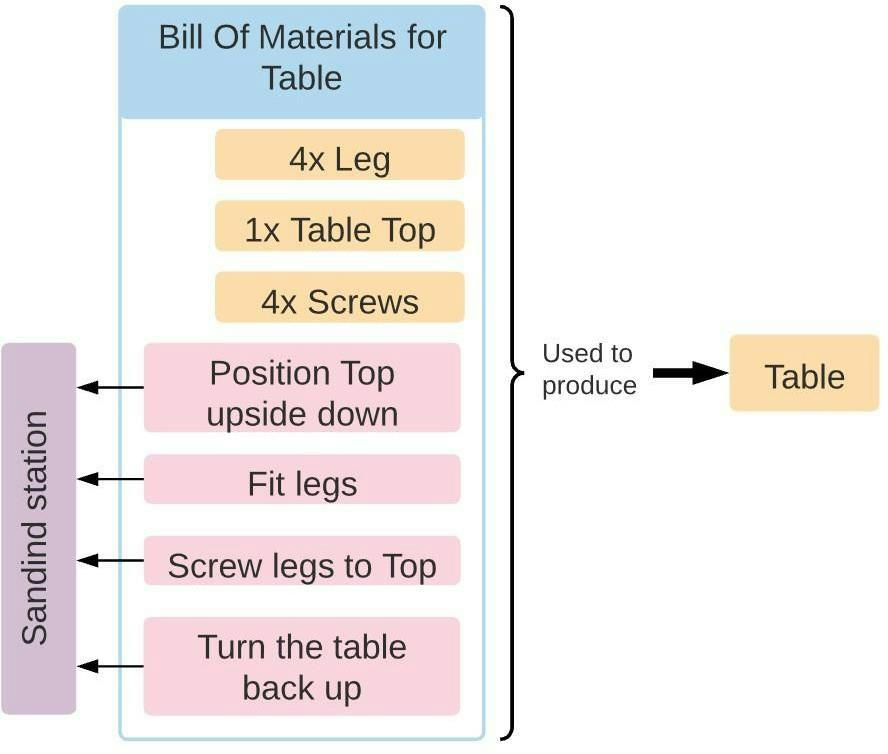
\includegraphics[width=426.24pt,height=361.9pt]{latexImage_3468b8e9ee10ae6dc6de804382fe3e9d.png}}
\end{picture}
\newpage
\begin{tikzpicture}[overlay]\path(0pt,0pt);\end{tikzpicture}
\begin{picture}(-5,0)(2.5,0)
\put(500.26,-727.616){\fontsize{12}{1}\usefont{T1}{ptm}{m}{n}\selectfont\color{color_29791}33}
\put(511.78,-727.616){\fontsize{12}{1}\usefont{T1}{ptm}{m}{n}\selectfont\color{color_29791} }
\put(63.024,-726.896){\fontsize{9.96}{1}\usefont{T1}{ptm}{m}{n}\selectfont\color{color_29791} }
\put(73.75,-528.45){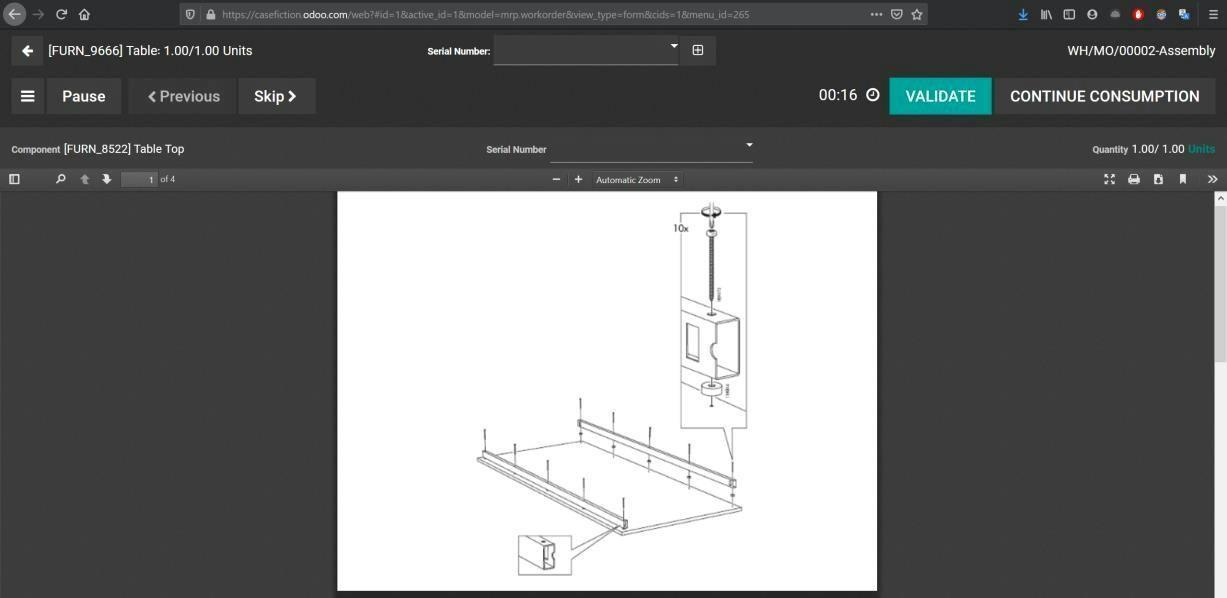
\includegraphics[width=441.53pt,height=215.25pt]{latexImage_43780e0d88746a17e6ff41379c0f3e4e.png}}
\put(503.98,-256.69){\fontsize{9.96}{1}\usefont{T1}{ptm}{m}{n}\selectfont\color{color_29791} }
\put(249.17,-278.05){\fontsize{12}{1}\usefont{T1}{ptm}{b}{n}\selectfont\color{color_29791}圖}
\put(261.17,-278.05){\fontsize{12}{1}\usefont{T1}{ptm}{b}{n}\selectfont\color{color_29791}25}
\put(273.17,-278.05){\fontsize{12}{1}\usefont{T1}{ptm}{b}{n}\selectfont\color{color_29791}簡化訂單圖}
\put(332.71,-278.05){\fontsize{12}{1}\usefont{T1}{ptm}{b}{n}\selectfont\color{color_29791} }
\put(63.024,-306.37){\fontsize{9.96}{1}\usefont{T1}{ptm}{b}{n}\selectfont\color{color_29791} }
\put(243.05,-548.67){\fontsize{12}{1}\usefont{T1}{ptm}{b}{n}\selectfont\color{color_29791}圖}
\put(255.05,-548.67){\fontsize{12}{1}\usefont{T1}{ptm}{b}{n}\selectfont\color{color_29791}26 WO}
\put(291.41,-548.67){\fontsize{12}{1}\usefont{T1}{ptm}{b}{n}\selectfont\color{color_29791}操作介面}
\put(338.83,-548.67){\fontsize{12}{1}\usefont{T1}{ptm}{b}{n}\selectfont\color{color_29791} }
\put(63.024,-569.43){\fontsize{12}{1}\usefont{T1}{ptm}{b}{n}\selectfont\color{color_29791} }
\put(63.024,-592.86){\fontsize{12}{1}\usefont{T1}{ptm}{b}{n}\selectfont\color{color_29791} }
\put(124.1,-613.62){\fontsize{12}{1}\usefont{T1}{ptm}{b}{n}\selectfont\color{color_29791}5.1.3.5.}
\put(160.1,-613.62){\fontsize{12}{1}\usefont{T1}{ptm}{b}{n}\selectfont\color{color_29791} }
\put(224.81,-613.62){\fontsize{12}{1}\usefont{T1}{ptm}{b}{n}\selectfont\color{color_29791}工程變更單}
\put(284.33,-613.62){\fontsize{12}{1}\usefont{T1}{ptm}{b}{n}\selectfont\color{color_29791} }
\put(63.024,-639.78){\fontsize{12}{1}\usefont{T1}{ptm}{b}{n}\selectfont\color{color_29791} }
\put(69.384,-657.3){\fontsize{12}{1}\usefont{T1}{ptm}{m}{n}\selectfont\color{color_29791}如第}
\put(93.14,-657.3){\fontsize{12}{1}\usefont{T1}{ptm}{m}{n}\selectfont\color{color_29791}2}
\put(99.02,-657.3){\fontsize{12}{1}\usefont{T1}{ptm}{m}{n}\selectfont\color{color_29791}章}
\put(110.9,-657.3){\fontsize{12}{1}\usefont{T1}{ptm}{m}{n}\selectfont\color{color_29791}開}
\put(122.78,-657.3){\fontsize{12}{1}\usefont{T1}{ptm}{m}{n}\selectfont\color{color_29791}頭}
\put(134.66,-657.3){\fontsize{12}{1}\usefont{T1}{ptm}{m}{n}\selectfont\color{color_29791}所}
\put(146.54,-657.3){\fontsize{12}{1}\usefont{T1}{ptm}{m}{n}\selectfont\color{color_29791}述,}
\put(170.42,-657.3){\fontsize{12}{1}\usefont{T1}{ptm}{m}{n}\selectfont\color{color_29791}O}
\put(178.94,-657.3){\fontsize{12}{1}\usefont{T1}{ptm}{m}{n}\selectfont\color{color_29791}d}
\put(184.82,-657.3){\fontsize{12}{1}\usefont{T1}{ptm}{m}{n}\selectfont\color{color_29791}oo}
\put(196.73,-657.3){\fontsize{12}{1}\usefont{T1}{ptm}{m}{n}\selectfont\color{color_29791}管理軟體主要將}
\put(279.89,-657.3){\fontsize{12}{1}\usefont{T1}{ptm}{m}{n}\selectfont\color{color_29791}P}
\put(286.49,-657.3){\fontsize{12}{1}\usefont{T1}{ptm}{m}{n}\selectfont\color{color_29791}LM}
\put(304.49,-657.3){\fontsize{12}{1}\usefont{T1}{ptm}{m}{n}\selectfont\color{color_29791}視為跟蹤變更和改}
\put(399.638,-657.3){\fontsize{12}{1}\usefont{T1}{ptm}{m}{n}\selectfont\color{color_29791}進的}
\put(423.506,-657.3){\fontsize{12}{1}\usefont{T1}{ptm}{m}{n}\selectfont\color{color_29791}工具。它的應用}
\put(506.86,-657.3){\fontsize{12}{1}\usefont{T1}{ptm}{m}{n}\selectfont\color{color_29791} }
\put(69.384,-675.18){\fontsize{12}{1}\usefont{T1}{ptm}{m}{n}\selectfont\color{color_29791}模組是}
\put(105.492,-675.18){\fontsize{12}{1}\usefont{T1}{ptm}{m}{n}\selectfont\color{color_29791}正常}
\put(129.6,-675.18){\fontsize{12}{1}\usefont{T1}{ptm}{m}{n}\selectfont\color{color_29791}製造流}
\put(165.708,-675.18){\fontsize{12}{1}\usefont{T1}{ptm}{m}{n}\selectfont\color{color_29791}程的}
\put(189.816,-675.18){\fontsize{12}{1}\usefont{T1}{ptm}{m}{n}\selectfont\color{color_29791}外部,}
\put(225.924,-675.18){\fontsize{12}{1}\usefont{T1}{ptm}{m}{n}\selectfont\color{color_29791}但充}
\put(250.032,-675.18){\fontsize{12}{1}\usefont{T1}{ptm}{m}{n}\selectfont\color{color_29791}當其擴}
\put(286.14,-675.18){\fontsize{12}{1}\usefont{T1}{ptm}{m}{n}\selectfont\color{color_29791}展。}
\put(310.248,-675.18){\fontsize{12}{1}\usefont{T1}{ptm}{m}{n}\selectfont\color{color_29791}其重點}
\put(346.356,-675.18){\fontsize{12}{1}\usefont{T1}{ptm}{m}{n}\selectfont\color{color_29791}專案}
\put(370.464,-675.18){\fontsize{12}{1}\usefont{T1}{ptm}{m}{n}\selectfont\color{color_29791}類是工}
\put(406.572,-675.18){\fontsize{12}{1}\usefont{T1}{ptm}{m}{n}\selectfont\color{color_29791}程變}
\put(430.68,-675.18){\fontsize{12}{1}\usefont{T1}{ptm}{m}{n}\selectfont\color{color_29791}更單}
\put(454.9,-675.18){\fontsize{12}{1}\usefont{T1}{ptm}{m}{n}\selectfont\color{color_29791} }
\put(460.9,-675.18){\fontsize{12}{1}\usefont{T1}{ptm}{m}{n}\selectfont\color{color_29791}(}
\put(472.9,-675.18){\fontsize{12}{1}\usefont{T1}{ptm}{m}{n}\selectfont\color{color_29791}ECO}
\put(496.9,-675.18){\fontsize{12}{1}\usefont{T1}{ptm}{m}{n}\selectfont\color{color_29791})。}
\put(521.02,-675.18){\fontsize{12}{1}\usefont{T1}{ptm}{m}{n}\selectfont\color{color_29791} }
\put(81.55,-256.65){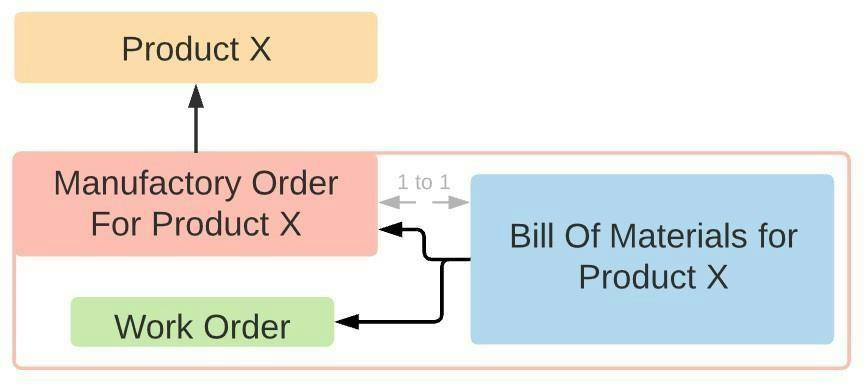
\includegraphics[width=422.24pt,height=187.65pt]{latexImage_9f5b36d988ebb22308ace2e7f44895d7.png}}
\end{picture}
\newpage
\begin{tikzpicture}[overlay]\path(0pt,0pt);\end{tikzpicture}
\begin{picture}(-5,0)(2.5,0)
\put(500.26,-727.616){\fontsize{12}{1}\usefont{T1}{ptm}{m}{n}\selectfont\color{color_29791}34}
\put(511.78,-727.616){\fontsize{12}{1}\usefont{T1}{ptm}{m}{n}\selectfont\color{color_29791} }
\put(63.024,-726.896){\fontsize{9.96}{1}\usefont{T1}{ptm}{m}{n}\selectfont\color{color_29791} }
\put(79.35,-449.1){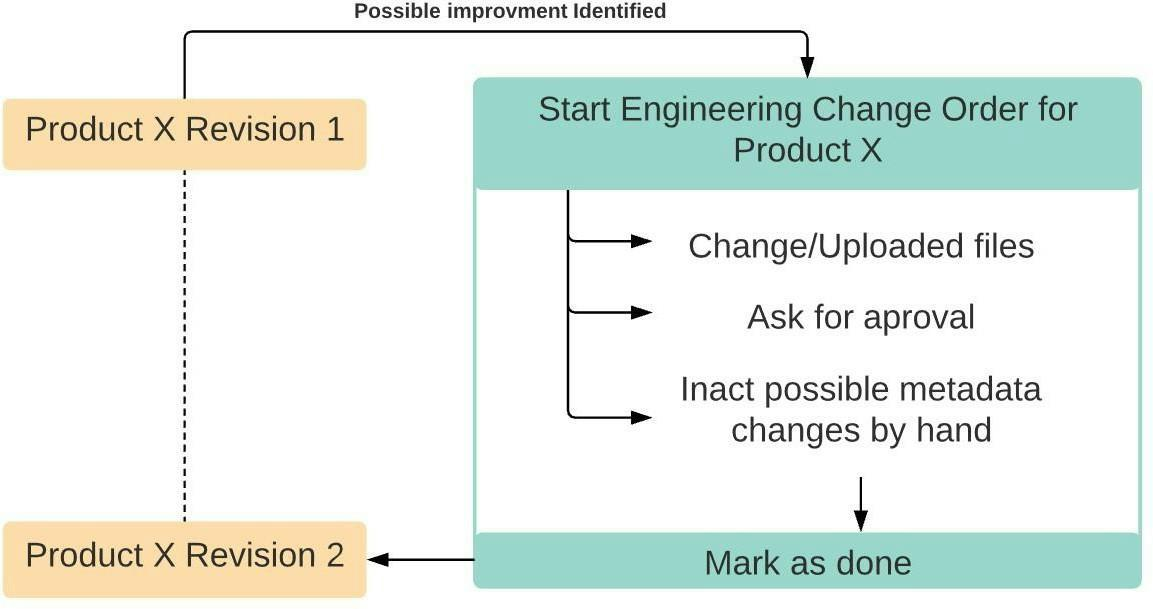
\includegraphics[width=432.3pt,height=228.35pt]{latexImage_7a738ea023a471b0281f7d26d709322d.png}}
\put(82.944,-71.96002){\fontsize{12}{1}\usefont{T1}{ptm}{m}{n}\selectfont\color{color_29791}E}
\put(90.024,-71.96002){\fontsize{12}{1}\usefont{T1}{ptm}{m}{n}\selectfont\color{color_29791}C}
\put(97.82401,-71.96002){\fontsize{12}{1}\usefont{T1}{ptm}{m}{n}\selectfont\color{color_29791}O}
\put(106.22,-71.96002){\fontsize{12}{1}\usefont{T1}{ptm}{m}{n}\selectfont\color{color_29791} }
\put(69.384,-88.06){\fontsize{12}{1}\usefont{T1}{ptm}{m}{n}\selectfont\color{color_29791}是一個專案類,它}
\put(164.532,-88.06){\fontsize{12}{1}\usefont{T1}{ptm}{m}{n}\selectfont\color{color_29791}概述}
\put(188.4,-88.06){\fontsize{12}{1}\usefont{T1}{ptm}{m}{n}\selectfont\color{color_29791}了對產品或將受更}
\put(283.548,-88.06){\fontsize{12}{1}\usefont{T1}{ptm}{m}{n}\selectfont\color{color_29791}改影}
\put(307.416,-88.06){\fontsize{12}{1}\usefont{T1}{ptm}{m}{n}\selectfont\color{color_29791}響的部件的擬議更}
\put(402.564,-88.06){\fontsize{12}{1}\usefont{T1}{ptm}{m}{n}\selectfont\color{color_29791}改。}
\put(426.432,-88.06){\fontsize{12}{1}\usefont{T1}{ptm}{m}{n}\selectfont\color{color_29791}換句話說,是}
\put(69.384,-106.06){\fontsize{12}{1}\usefont{T1}{ptm}{m}{n}\selectfont\color{color_29791}與給定產品相關的}
\put(164.532,-106.06){\fontsize{12}{1}\usefont{T1}{ptm}{m}{n}\selectfont\color{color_29791}每個}
\put(188.4,-106.06){\fontsize{12}{1}\usefont{T1}{ptm}{m}{n}\selectfont\color{color_29791}人的中央資訊中心}
\put(283.548,-106.06){\fontsize{12}{1}\usefont{T1}{ptm}{m}{n}\selectfont\color{color_29791}。}
\put(295.61,-106.06){\fontsize{12}{1}\usefont{T1}{ptm}{m}{n}\selectfont\color{color_29791} }
\put(63.024,-124.3){\fontsize{12}{1}\usefont{T1}{ptm}{m}{n}\selectfont\color{color_29791} }
\put(82.944,-139.78){\fontsize{12}{1}\usefont{T1}{ptm}{m}{n}\selectfont\color{color_29791}這個想法是發出需要更改產品項}
\put(250.97,-139.78){\fontsize{12}{1}\usefont{T1}{ptm}{m}{n}\selectfont\color{color_29791}或}
\put(262.49,-139.78){\fontsize{12}{1}\usefont{T1}{ptm}{m}{n}\selectfont\color{color_29791} }
\put(485.26,-139.78){\fontsize{12}{1}\usefont{T1}{ptm}{m}{n}\selectfont\color{color_29791}B}
\put(493.06,-139.78){\fontsize{12}{1}\usefont{T1}{ptm}{m}{n}\selectfont\color{color_29791}O}
\put(501.46,-139.78){\fontsize{12}{1}\usefont{T1}{ptm}{m}{n}\selectfont\color{color_29791}M}
\put(511.9,-139.78){\fontsize{12}{1}\usefont{T1}{ptm}{m}{n}\selectfont\color{color_29791} }
\put(69.384,-157.66){\fontsize{12}{1}\usefont{T1}{ptm}{m}{n}\selectfont\color{color_29791}項的信號,保留與更改}
\put(189.492,-157.66){\fontsize{12}{1}\usefont{T1}{ptm}{m}{n}\selectfont\color{color_29791}相關的檔並應用更改,}
\put(309.6,-157.66){\fontsize{12}{1}\usefont{T1}{ptm}{m}{n}\selectfont\color{color_29791}或者至少發出已實施更}
\put(429.708,-157.66){\fontsize{12}{1}\usefont{T1}{ptm}{m}{n}\selectfont\color{color_29791}改的信號,同}
\put(69.384,-175.66){\fontsize{12}{1}\usefont{T1}{ptm}{m}{n}\selectfont\color{color_29791}時保留所有先前更改的}
\put(189.492,-175.66){\fontsize{12}{1}\usefont{T1}{ptm}{m}{n}\selectfont\color{color_29791}歷史記錄。所有這些都}
\put(309.6,-175.66){\fontsize{12}{1}\usefont{T1}{ptm}{m}{n}\selectfont\color{color_29791}在未來非常有用,並作}
\put(429.708,-175.66){\fontsize{12}{1}\usefont{T1}{ptm}{m}{n}\selectfont\color{color_29791}為簡化產品開}
\put(69.384,-193.54){\fontsize{12}{1}\usefont{T1}{ptm}{m}{n}\selectfont\color{color_29791}發和説明改進產品}
\put(164.42,-193.54){\fontsize{12}{1}\usefont{T1}{ptm}{m}{n}\selectfont\color{color_29791}/}
\put(167.78,-193.54){\fontsize{12}{1}\usefont{T1}{ptm}{m}{n}\selectfont\color{color_29791}生}
\put(179.66,-193.54){\fontsize{12}{1}\usefont{T1}{ptm}{m}{n}\selectfont\color{color_29791}產的}
\put(203.54,-193.54){\fontsize{12}{1}\usefont{T1}{ptm}{m}{n}\selectfont\color{color_29791}過}
\put(215.42,-193.54){\fontsize{12}{1}\usefont{T1}{ptm}{m}{n}\selectfont\color{color_29791}程}
\put(227.3,-193.54){\fontsize{12}{1}\usefont{T1}{ptm}{m}{n}\selectfont\color{color_29791}。}
\put(239.33,-193.54){\fontsize{12}{1}\usefont{T1}{ptm}{m}{n}\selectfont\color{color_29791} }
\put(63.024,-216.82){\fontsize{9.96}{1}\usefont{T1}{ptm}{m}{n}\selectfont\color{color_29791} }
\put(229.97,-472.95){\fontsize{12}{1}\usefont{T1}{ptm}{b}{n}\selectfont\color{color_29791}圖}
\put(241.85,-472.95){\fontsize{12}{1}\usefont{T1}{ptm}{b}{n}\selectfont\color{color_29791}27}
\put(253.61,-472.95){\fontsize{12}{1}\usefont{T1}{ptm}{b}{n}\selectfont\color{color_29791}簡化的}
\put(289.25,-472.95){\fontsize{12}{1}\usefont{T1}{ptm}{b}{n}\selectfont\color{color_29791}E}
\put(297.17,-472.95){\fontsize{12}{1}\usefont{T1}{ptm}{b}{n}\selectfont\color{color_29791}C}
\put(305.69,-472.95){\fontsize{12}{1}\usefont{T1}{ptm}{b}{n}\selectfont\color{color_29791}O}
\put(314.95,-472.95){\fontsize{12}{1}\usefont{T1}{ptm}{b}{n}\selectfont\color{color_29791}功能圖}
\put(350.35,-472.95){\fontsize{12}{1}\usefont{T1}{ptm}{b}{n}\selectfont\color{color_29791} }
\put(87.38,-505.83){\fontsize{14.04}{1}\usefont{T1}{ptm}{b}{n}\selectfont\color{color_29791}5}
\put(94.44212,-505.83){\fontsize{14.04}{1}\usefont{T1}{ptm}{b}{n}\selectfont\color{color_29791}.2.}
\put(108.38,-505.83){\fontsize{14.04}{1}\usefont{T1}{ptm}{b}{n}\selectfont\color{color_29791} }
\put(111.74,-505.83){\fontsize{14.04}{1}\usefont{T1}{ptm}{b}{n}\selectfont\color{color_29791}開}
\put(125.6536,-505.83){\fontsize{14.04}{1}\usefont{T1}{ptm}{b}{n}\selectfont\color{color_29791}始}
\put(139.455,-505.83){\fontsize{14.04}{1}\usefont{T1}{ptm}{b}{n}\selectfont\color{color_29791}模}
\put(153.3686,-505.83){\fontsize{14.04}{1}\usefont{T1}{ptm}{b}{n}\selectfont\color{color_29791}擬}
\put(167.18,-505.83){\fontsize{14.04}{1}\usefont{T1}{ptm}{b}{n}\selectfont\color{color_29791} }
\put(105.38,-550.35){\fontsize{12.81913}{1}\usefont{T1}{ptm}{b}{n}\selectfont\color{color_29791}5.}
\put(114.9648,-550.35){\fontsize{12.81913}{1}\usefont{T1}{ptm}{b}{n}\selectfont\color{color_29791}2}
\put(121.4307,-550.35){\fontsize{12.81913}{1}\usefont{T1}{ptm}{b}{n}\selectfont\color{color_29791}.}
\put(124.5495,-550.35){\fontsize{12.81913}{1}\usefont{T1}{ptm}{b}{n}\selectfont\color{color_29791}1}
\put(131.0154,-550.35){\fontsize{12.81913}{1}\usefont{T1}{ptm}{b}{n}\selectfont\color{color_29791}.}
\put(134.3,-550.35){\fontsize{12.83539}{1}\usefont{T1}{ptm}{b}{n}\selectfont\color{color_29791} }
\put(137.66,-550.35){\fontsize{12.96}{1}\usefont{T1}{ptm}{b}{n}\selectfont\color{color_29791}為模擬選擇的軟體選}
\put(253.3237,-550.35){\fontsize{12.96}{1}\usefont{T1}{ptm}{b}{n}\selectfont\color{color_29791}項}
\put(266.21,-550.35){\fontsize{12.96}{1}\usefont{T1}{ptm}{b}{n}\selectfont\color{color_29791} }
\put(82.944,-578.82){\fontsize{12}{1}\usefont{T1}{ptm}{m}{n}\selectfont\color{color_29791}對於此類比,已決}
\put(178.092,-578.82){\fontsize{12}{1}\usefont{T1}{ptm}{m}{n}\selectfont\color{color_29791}定通}
\put(201.96,-578.82){\fontsize{12}{1}\usefont{T1}{ptm}{m}{n}\selectfont\color{color_29791}過其基於}
\put(249.53,-578.82){\fontsize{12}{1}\usefont{T1}{ptm}{m}{n}\selectfont\color{color_29791}W}
\put(260.81,-578.82){\fontsize{12}{1}\usefont{T1}{ptm}{m}{n}\selectfont\color{color_29791}e}
\put(265.97,-578.82){\fontsize{12}{1}\usefont{T1}{ptm}{m}{n}\selectfont\color{color_29791}b}
\put(271.85,-578.82){\fontsize{12}{1}\usefont{T1}{ptm}{m}{n}\selectfont\color{color_29791}的}
\put(283.73,-578.82){\fontsize{12}{1}\usefont{T1}{ptm}{m}{n}\selectfont\color{color_29791}在}
\put(295.61,-578.82){\fontsize{12}{1}\usefont{T1}{ptm}{m}{n}\selectfont\color{color_29791}線服務}
\put(331.49,-578.82){\fontsize{12}{1}\usefont{T1}{ptm}{m}{n}\selectfont\color{color_29791}對}
\put(343.39,-578.82){\fontsize{12}{1}\usefont{T1}{ptm}{m}{n}\selectfont\color{color_29791}O}
\put(351.91,-578.82){\fontsize{12}{1}\usefont{T1}{ptm}{m}{n}\selectfont\color{color_29791}d}
\put(357.79,-578.82){\fontsize{12}{1}\usefont{T1}{ptm}{m}{n}\selectfont\color{color_29791}o}
\put(363.67,-578.82){\fontsize{12}{1}\usefont{T1}{ptm}{m}{n}\selectfont\color{color_29791}o}
\put(369.55,-578.82){\fontsize{12}{1}\usefont{T1}{ptm}{m}{n}\selectfont\color{color_29791}軟體}
\put(393.43,-578.82){\fontsize{12}{1}\usefont{T1}{ptm}{m}{n}\selectfont\color{color_29791}進}
\put(405.31,-578.82){\fontsize{12}{1}\usefont{T1}{ptm}{m}{n}\selectfont\color{color_29791}行}
\put(417.19,-578.82){\fontsize{12}{1}\usefont{T1}{ptm}{m}{n}\selectfont\color{color_29791}最}
\put(429.07,-578.82){\fontsize{12}{1}\usefont{T1}{ptm}{m}{n}\selectfont\color{color_29791}佳評}
\put(452.95,-578.82){\fontsize{12}{1}\usefont{T1}{ptm}{m}{n}\selectfont\color{color_29791}估}
\put(464.83,-578.82){\fontsize{12}{1}\usefont{T1}{ptm}{m}{n}\selectfont\color{color_29791}。}
\put(476.71,-578.82){\fontsize{12}{1}\usefont{T1}{ptm}{m}{n}\selectfont\color{color_29791}選}
\put(488.59,-578.82){\fontsize{12}{1}\usefont{T1}{ptm}{m}{n}\selectfont\color{color_29791}擇}
\put(69.384,-596.82){\fontsize{12}{1}\usefont{T1}{ptm}{m}{n}\selectfont\color{color_29791}不使用該軟體的社}
\put(164.532,-596.82){\fontsize{12}{1}\usefont{T1}{ptm}{m}{n}\selectfont\color{color_29791}區版}
\put(188.4,-596.82){\fontsize{12}{1}\usefont{T1}{ptm}{m}{n}\selectfont\color{color_29791}的原因如下:}
\put(259.85,-596.82){\fontsize{12}{1}\usefont{T1}{ptm}{m}{n}\selectfont\color{color_29791} }
\put(63.024,-615.78){\fontsize{12}{1}\usefont{T1}{ptm}{m}{n}\selectfont\color{color_29791} }
\put(102.26,-631.5){\fontsize{12}{1}\usefont{T1}{ptm}{m}{n}\selectfont\color{color_29791}}
\put(112.94,-631.5){\fontsize{12}{1}\usefont{T1}{uarial}{m}{n}\selectfont\color{color_29791} }
\put(120.26,-631.5){\fontsize{12}{1}\usefont{T1}{ptm}{m}{n}\selectfont\color{color_29791}使用基}
\put(156.26,-631.5){\fontsize{12}{1}\usefont{T1}{ptm}{m}{n}\selectfont\color{color_29791}於}
\put(167.78,-631.5){\fontsize{12}{1}\usefont{T1}{ptm}{m}{n}\selectfont\color{color_29791} }
\put(490.9,-631.5){\fontsize{12}{1}\usefont{T1}{ptm}{m}{n}\selectfont\color{color_29791}Web}
\put(512.86,-631.5){\fontsize{12}{1}\usefont{T1}{ptm}{m}{n}\selectfont\color{color_29791} }
\put(120.26,-649.38){\fontsize{12}{1}\usefont{T1}{ptm}{m}{n}\selectfont\color{color_29791}的服務作為本地或}
\put(215.408,-649.38){\fontsize{12}{1}\usefont{T1}{ptm}{m}{n}\selectfont\color{color_29791}遠端}
\put(239.276,-649.38){\fontsize{12}{1}\usefont{T1}{ptm}{m}{n}\selectfont\color{color_29791}管理伺服器的實用}
\put(334.424,-649.38){\fontsize{12}{1}\usefont{T1}{ptm}{m}{n}\selectfont\color{color_29791}性。}
\put(358.292,-649.38){\fontsize{12}{1}\usefont{T1}{ptm}{m}{n}\selectfont\color{color_29791}儘管社區應用程式}
\put(453.44,-649.38){\fontsize{12}{1}\usefont{T1}{ptm}{m}{n}\selectfont\color{color_29791}作為}
\put(477.308,-649.38){\fontsize{12}{1}\usefont{T1}{ptm}{m}{n}\selectfont\color{color_29791}這項}
\put(120.26,-667.26){\fontsize{12}{1}\usefont{T1}{ptm}{m}{n}\selectfont\color{color_29791}工作研}
\put(156.14,-667.26){\fontsize{12}{1}\usefont{T1}{ptm}{m}{n}\selectfont\color{color_29791}究的一}
\put(192.02,-667.26){\fontsize{12}{1}\usefont{T1}{ptm}{m}{n}\selectfont\color{color_29791}部分}
\put(215.9,-667.26){\fontsize{12}{1}\usefont{T1}{ptm}{m}{n}\selectfont\color{color_29791}進行}
\put(239.78,-667.26){\fontsize{12}{1}\usefont{T1}{ptm}{m}{n}\selectfont\color{color_29791}了測試}
\put(275.66,-667.26){\fontsize{12}{1}\usefont{T1}{ptm}{m}{n}\selectfont\color{color_29791},並且}
\put(311.54,-667.26){\fontsize{12}{1}\usefont{T1}{ptm}{m}{n}\selectfont\color{color_29791}被認}
\put(335.42,-667.26){\fontsize{12}{1}\usefont{T1}{ptm}{m}{n}\selectfont\color{color_29791}為是}
\put(359.3,-667.26){\fontsize{12}{1}\usefont{T1}{ptm}{m}{n}\selectfont\color{color_29791}一個非}
\put(395.18,-667.26){\fontsize{12}{1}\usefont{T1}{ptm}{m}{n}\selectfont\color{color_29791}常初學}
\put(431.06,-667.26){\fontsize{12}{1}\usefont{T1}{ptm}{m}{n}\selectfont\color{color_29791}者友}
\put(454.94,-667.26){\fontsize{12}{1}\usefont{T1}{ptm}{m}{n}\selectfont\color{color_29791}好的}
\put(478.82,-667.26){\fontsize{12}{1}\usefont{T1}{ptm}{m}{n}\selectfont\color{color_29791}伺服}
\put(502.78,-667.26){\fontsize{12}{1}\usefont{T1}{ptm}{m}{n}\selectfont\color{color_29791} }
\put(120.26,-685.136){\fontsize{12}{1}\usefont{T1}{ptm}{m}{n}\selectfont\color{color_29791}器應用程式,但事}
\put(215.408,-685.136){\fontsize{12}{1}\usefont{T1}{ptm}{m}{n}\selectfont\color{color_29791}實是}
\put(239.276,-685.136){\fontsize{12}{1}\usefont{T1}{ptm}{m}{n}\selectfont\color{color_29791},託管伺服器本身}
\put(334.424,-685.136){\fontsize{12}{1}\usefont{T1}{ptm}{m}{n}\selectfont\color{color_29791}就是}
\put(358.292,-685.136){\fontsize{12}{1}\usefont{T1}{ptm}{m}{n}\selectfont\color{color_29791}一項需要經驗和知}
\put(453.44,-685.136){\fontsize{12}{1}\usefont{T1}{ptm}{m}{n}\selectfont\color{color_29791}識的}
\put(477.308,-685.136){\fontsize{12}{1}\usefont{T1}{ptm}{m}{n}\selectfont\color{color_29791}工作。}
\put(120.26,-702.896){\fontsize{12}{1}\usefont{T1}{ptm}{m}{n}\selectfont\color{color_29791}關於這種應用,市}
\put(215.408,-702.896){\fontsize{12}{1}\usefont{T1}{ptm}{m}{n}\selectfont\color{color_29791}場已}
\put(239.276,-702.896){\fontsize{12}{1}\usefont{T1}{ptm}{m}{n}\selectfont\color{color_29791}經轉向產品即服務}
\put(334.424,-702.896){\fontsize{12}{1}\usefont{T1}{ptm}{m}{n}\selectfont\color{color_29791},這}
\put(358.292,-702.896){\fontsize{12}{1}\usefont{T1}{ptm}{m}{n}\selectfont\color{color_29791}是有充分理由的。}
\put(453.44,-702.896){\fontsize{12}{1}\usefont{T1}{ptm}{m}{n}\selectfont\color{color_29791}在撰}
\put(477.308,-702.896){\fontsize{12}{1}\usefont{T1}{ptm}{m}{n}\selectfont\color{color_29791}寫本}
\put(501.22,-702.896){\fontsize{12}{1}\usefont{T1}{ptm}{m}{n}\selectfont\color{color_29791} }
\end{picture}
\newpage
\begin{tikzpicture}[overlay]\path(0pt,0pt);\end{tikzpicture}
\begin{picture}(-5,0)(2.5,0)
\put(500.26,-727.616){\fontsize{12}{1}\usefont{T1}{ptm}{m}{n}\selectfont\color{color_29791}35}
\put(511.78,-727.616){\fontsize{12}{1}\usefont{T1}{ptm}{m}{n}\selectfont\color{color_29791} }
\put(63.024,-726.896){\fontsize{9.96}{1}\usefont{T1}{ptm}{m}{n}\selectfont\color{color_29791} }
\put(120.26,-72.44){\fontsize{12}{1}\usefont{T1}{ptm}{m}{n}\selectfont\color{color_29791}文時,}
\put(155.9,-72.44){\fontsize{12}{1}\usefont{T1}{ptm}{m}{n}\selectfont\color{color_29791}C}
\put(163.82,-72.44){\fontsize{12}{1}\usefont{T1}{ptm}{m}{n}\selectfont\color{color_29791}O}
\put(172.34,-72.44){\fontsize{12}{1}\usefont{T1}{ptm}{m}{n}\selectfont\color{color_29791}VI}
\put(184.82,-72.44){\fontsize{12}{1}\usefont{T1}{ptm}{m}{n}\selectfont\color{color_29791}D}
\put(193.37,-72.44){\fontsize{12}{1}\usefont{T1}{ptm}{m}{n}\selectfont\color{color_29791}-}
\put(197.21,-72.44){\fontsize{12}{1}\usefont{T1}{ptm}{m}{n}\selectfont\color{color_29791}19}
\put(208.85,-72.44){\fontsize{12}{1}\usefont{T1}{ptm}{m}{n}\selectfont\color{color_29791} }
\put(235.85,-72.44){\fontsize{12}{1}\usefont{T1}{ptm}{m}{n}\selectfont\color{color_29791}大流行迫使許多員工遠端工作,並向市場表}
\put(463.9,-72.44){\fontsize{12}{1}\usefont{T1}{ptm}{m}{n}\selectfont\color{color_29791}明}
\put(475.42,-72.44){\fontsize{12}{1}\usefont{T1}{ptm}{m}{n}\selectfont\color{color_29791} }
\put(501.7,-72.44){\fontsize{12}{1}\usefont{T1}{ptm}{m}{n}\selectfont\color{color_29791}IT}
\put(512.5,-72.44){\fontsize{12}{1}\usefont{T1}{ptm}{m}{n}\selectfont\color{color_29791} }
\put(120.26,-90.34003){\fontsize{12}{1}\usefont{T1}{ptm}{m}{n}\selectfont\color{color_29791}不是一項簡單的工}
\put(215.408,-90.34003){\fontsize{12}{1}\usefont{T1}{ptm}{m}{n}\selectfont\color{color_29791}作,}
\put(239.33,-90.34003){\fontsize{12}{1}\usefont{T1}{ptm}{m}{n}\selectfont\color{color_29791}Web}
\put(261.53,-90.34003){\fontsize{12}{1}\usefont{T1}{ptm}{m}{n}\selectfont\color{color_29791} }
\put(265.97,-90.34003){\fontsize{12}{1}\usefont{T1}{ptm}{m}{n}\selectfont\color{color_29791}服務是一個有吸引}
\put(360.89,-90.34003){\fontsize{12}{1}\usefont{T1}{ptm}{m}{n}\selectfont\color{color_29791}力的選擇。}
\put(420.19,-90.34003){\fontsize{12}{1}\usefont{T1}{ptm}{m}{n}\selectfont\color{color_29791} }
\put(63.024,-109.66){\fontsize{12}{1}\usefont{T1}{ptm}{m}{n}\selectfont\color{color_29791} }
\put(102.26,-125.26){\fontsize{12}{1}\usefont{T1}{ptm}{m}{n}\selectfont\color{color_29791}}
\put(112.94,-125.26){\fontsize{12}{1}\usefont{T1}{uarial}{m}{n}\selectfont\color{color_29791} }
\put(120.26,-125.26){\fontsize{12}{1}\usefont{T1}{ptm}{m}{n}\selectfont\color{color_29791}缺少}
\put(144.62,-125.26){\fontsize{12}{1}\usefont{T1}{ptm}{m}{n}\selectfont\color{color_29791}O}
\put(153.14,-125.26){\fontsize{12}{1}\usefont{T1}{ptm}{m}{n}\selectfont\color{color_29791}d}
\put(159.02,-125.26){\fontsize{12}{1}\usefont{T1}{ptm}{m}{n}\selectfont\color{color_29791}oo}
\put(171.14,-125.26){\fontsize{12}{1}\usefont{T1}{ptm}{m}{n}\selectfont\color{color_29791}社}
\put(183.368,-125.26){\fontsize{12}{1}\usefont{T1}{ptm}{m}{n}\selectfont\color{color_29791}區}
\put(195.476,-125.26){\fontsize{12}{1}\usefont{T1}{ptm}{m}{n}\selectfont\color{color_29791}版}
\put(207.704,-125.26){\fontsize{12}{1}\usefont{T1}{ptm}{m}{n}\selectfont\color{color_29791}的}
\put(219.932,-125.26){\fontsize{12}{1}\usefont{T1}{ptm}{m}{n}\selectfont\color{color_29791}官}
\put(232.16,-125.26){\fontsize{12}{1}\usefont{T1}{ptm}{m}{n}\selectfont\color{color_29791}方}
\put(244.37,-125.26){\fontsize{12}{1}\usefont{T1}{ptm}{m}{n}\selectfont\color{color_29791}O}
\put(252.89,-125.26){\fontsize{12}{1}\usefont{T1}{ptm}{m}{n}\selectfont\color{color_29791}d}
\put(258.77,-125.26){\fontsize{12}{1}\usefont{T1}{ptm}{m}{n}\selectfont\color{color_29791}oo}
\put(270.65,-125.26){\fontsize{12}{1}\usefont{T1}{ptm}{m}{n}\selectfont\color{color_29791}P}
\put(277.25,-125.26){\fontsize{12}{1}\usefont{T1}{ptm}{m}{n}\selectfont\color{color_29791}L}
\put(284.45,-125.26){\fontsize{12}{1}\usefont{T1}{ptm}{m}{n}\selectfont\color{color_29791}M}
\put(295.37,-125.26){\fontsize{12}{1}\usefont{T1}{ptm}{m}{n}\selectfont\color{color_29791}應}
\put(307.478,-125.26){\fontsize{12}{1}\usefont{T1}{ptm}{m}{n}\selectfont\color{color_29791}用}
\put(319.706,-125.26){\fontsize{12}{1}\usefont{T1}{ptm}{m}{n}\selectfont\color{color_29791}程}
\put(331.934,-125.26){\fontsize{12}{1}\usefont{T1}{ptm}{m}{n}\selectfont\color{color_29791}式}
\put(344.162,-125.26){\fontsize{12}{1}\usefont{T1}{ptm}{m}{n}\selectfont\color{color_29791}。}
\put(356.27,-125.26){\fontsize{12}{1}\usefont{T1}{ptm}{m}{n}\selectfont\color{color_29791}儘}
\put(368.498,-125.26){\fontsize{12}{1}\usefont{T1}{ptm}{m}{n}\selectfont\color{color_29791}管}
\put(380.71,-125.26){\fontsize{12}{1}\usefont{T1}{ptm}{m}{n}\selectfont\color{color_29791}O}
\put(389.23,-125.26){\fontsize{12}{1}\usefont{T1}{ptm}{m}{n}\selectfont\color{color_29791}do}
\put(401.11,-125.26){\fontsize{12}{1}\usefont{T1}{ptm}{m}{n}\selectfont\color{color_29791}o}
\put(407.35,-125.26){\fontsize{12}{1}\usefont{T1}{ptm}{m}{n}\selectfont\color{color_29791}的}
\put(419.458,-125.26){\fontsize{12}{1}\usefont{T1}{ptm}{m}{n}\selectfont\color{color_29791}社}
\put(431.686,-125.26){\fontsize{12}{1}\usefont{T1}{ptm}{m}{n}\selectfont\color{color_29791}區}
\put(443.914,-125.26){\fontsize{12}{1}\usefont{T1}{ptm}{m}{n}\selectfont\color{color_29791}版}
\put(456.142,-125.26){\fontsize{12}{1}\usefont{T1}{ptm}{m}{n}\selectfont\color{color_29791}有}
\put(468.25,-125.26){\fontsize{12}{1}\usefont{T1}{ptm}{m}{n}\selectfont\color{color_29791}大}
\put(480.478,-125.26){\fontsize{12}{1}\usefont{T1}{ptm}{m}{n}\selectfont\color{color_29791}量}
\put(492.586,-125.26){\fontsize{12}{1}\usefont{T1}{ptm}{m}{n}\selectfont\color{color_29791}的}
\put(120.26,-143.14){\fontsize{12}{1}\usefont{T1}{ptm}{m}{n}\selectfont\color{color_29791}社區應用程式,但這些}
\put(240.368,-143.14){\fontsize{12}{1}\usefont{T1}{ptm}{m}{n}\selectfont\color{color_29791}應用程式的組織、描述}
\put(360.476,-143.14){\fontsize{12}{1}\usefont{T1}{ptm}{m}{n}\selectfont\color{color_29791}、集成和支援充其量只}
\put(480.584,-143.14){\fontsize{12}{1}\usefont{T1}{ptm}{m}{n}\selectfont\color{color_29791}能被}
\put(120.26,-161.02){\fontsize{12}{1}\usefont{T1}{ptm}{m}{n}\selectfont\color{color_29791}發現。與其依賴可能跟}
\put(240.368,-161.02){\fontsize{12}{1}\usefont{T1}{ptm}{m}{n}\selectfont\color{color_29791}不上主要軟體的應用程}
\put(360.476,-161.02){\fontsize{12}{1}\usefont{T1}{ptm}{m}{n}\selectfont\color{color_29791}式,不如決定如果基於}
\put(480.584,-161.02){\fontsize{12}{1}\usefont{T1}{ptm}{m}{n}\selectfont\color{color_29791}官方}
\put(120.26,-178.9){\fontsize{12}{1}\usefont{T1}{ptm}{m}{n}\selectfont\color{color_29791}應用程式,對平臺評估}
\put(240.368,-178.9){\fontsize{12}{1}\usefont{T1}{ptm}{m}{n}\selectfont\color{color_29791}會更公平。也就是說,}
\put(360.476,-178.9){\fontsize{12}{1}\usefont{T1}{ptm}{m}{n}\selectfont\color{color_29791}僅僅依靠運氣來決定未}
\put(480.584,-178.9){\fontsize{12}{1}\usefont{T1}{ptm}{m}{n}\selectfont\color{color_29791}來如}
\put(120.26,-196.78){\fontsize{12}{1}\usefont{T1}{ptm}{m}{n}\selectfont\color{color_29791}何支援它,就拼湊}
\put(215.408,-196.78){\fontsize{12}{1}\usefont{T1}{ptm}{m}{n}\selectfont\color{color_29791}出一}
\put(239.276,-196.78){\fontsize{12}{1}\usefont{T1}{ptm}{m}{n}\selectfont\color{color_29791}個免費的解決方案}
\put(334.424,-196.78){\fontsize{12}{1}\usefont{T1}{ptm}{m}{n}\selectfont\color{color_29791}是非}
\put(358.292,-196.78){\fontsize{12}{1}\usefont{T1}{ptm}{m}{n}\selectfont\color{color_29791}常徒勞的。}
\put(417.79,-196.78){\fontsize{12}{1}\usefont{T1}{ptm}{m}{n}\selectfont\color{color_29791}P}
\put(424.39,-196.78){\fontsize{12}{1}\usefont{T1}{ptm}{m}{n}\selectfont\color{color_29791}L}
\put(431.59,-196.78){\fontsize{12}{1}\usefont{T1}{ptm}{m}{n}\selectfont\color{color_29791}M}
\put(442.3,-196.78){\fontsize{12}{1}\usefont{T1}{ptm}{m}{n}\selectfont\color{color_29791} }
\put(120.26,-214.66){\fontsize{12}{1}\usefont{T1}{ptm}{m}{n}\selectfont\color{color_29791}是這裡}
\put(156.14,-214.66){\fontsize{12}{1}\usefont{T1}{ptm}{m}{n}\selectfont\color{color_29791}的重點}
\put(192.02,-214.66){\fontsize{12}{1}\usefont{T1}{ptm}{m}{n}\selectfont\color{color_29791},所}
\put(215.9,-214.66){\fontsize{12}{1}\usefont{T1}{ptm}{m}{n}\selectfont\color{color_29791}以這}
\put(239.78,-214.66){\fontsize{12}{1}\usefont{T1}{ptm}{m}{n}\selectfont\color{color_29791}是一個}
\put(275.66,-214.66){\fontsize{12}{1}\usefont{T1}{ptm}{m}{n}\selectfont\color{color_29791}不容置}
\put(311.54,-214.66){\fontsize{12}{1}\usefont{T1}{ptm}{m}{n}\selectfont\color{color_29791}疑的}
\put(335.42,-214.66){\fontsize{12}{1}\usefont{T1}{ptm}{m}{n}\selectfont\color{color_29791}情況}
\put(359.3,-214.66){\fontsize{12}{1}\usefont{T1}{ptm}{m}{n}\selectfont\color{color_29791}。}
\put(371.35,-214.66){\fontsize{12}{1}\usefont{T1}{ptm}{m}{n}\selectfont\color{color_29791} }
\put(63.024,-232.42){\fontsize{12}{1}\usefont{T1}{ptm}{m}{n}\selectfont\color{color_29791} }
\put(82.944,-248.05){\fontsize{12}{1}\usefont{T1}{ptm}{m}{n}\selectfont\color{color_29791}在撰寫本文時,}
\put(166.22,-248.05){\fontsize{12}{1}\usefont{T1}{ptm}{m}{n}\selectfont\color{color_29791}O}
\put(174.74,-248.05){\fontsize{12}{1}\usefont{T1}{ptm}{m}{n}\selectfont\color{color_29791}d}
\put(180.62,-248.05){\fontsize{12}{1}\usefont{T1}{ptm}{m}{n}\selectfont\color{color_29791}o}
\put(186.5,-248.05){\fontsize{12}{1}\usefont{T1}{ptm}{m}{n}\selectfont\color{color_29791}o}
\put(192.41,-248.05){\fontsize{12}{1}\usefont{T1}{ptm}{m}{n}\selectfont\color{color_29791}允許}
\put(216.29,-248.05){\fontsize{12}{1}\usefont{T1}{ptm}{m}{n}\selectfont\color{color_29791}您}
\put(228.17,-248.05){\fontsize{12}{1}\usefont{T1}{ptm}{m}{n}\selectfont\color{color_29791}選}
\put(240.05,-248.05){\fontsize{12}{1}\usefont{T1}{ptm}{m}{n}\selectfont\color{color_29791}擇}
\put(251.93,-248.05){\fontsize{12}{1}\usefont{T1}{ptm}{m}{n}\selectfont\color{color_29791}其}
\put(263.81,-248.05){\fontsize{12}{1}\usefont{T1}{ptm}{m}{n}\selectfont\color{color_29791}額}
\put(275.69,-248.05){\fontsize{12}{1}\usefont{T1}{ptm}{m}{n}\selectfont\color{color_29791}外}
\put(287.57,-248.05){\fontsize{12}{1}\usefont{T1}{ptm}{m}{n}\selectfont\color{color_29791}功能}
\put(311.45,-248.05){\fontsize{12}{1}\usefont{T1}{ptm}{m}{n}\selectfont\color{color_29791}之一}
\put(335.33,-248.05){\fontsize{12}{1}\usefont{T1}{ptm}{m}{n}\selectfont\color{color_29791},}
\put(347.2101,-248.05){\fontsize{12}{1}\usefont{T1}{ptm}{m}{n}\selectfont\color{color_29791}例}
\put(359.0901,-248.05){\fontsize{12}{1}\usefont{T1}{ptm}{m}{n}\selectfont\color{color_29791}如}
\put(370.99,-248.05){\fontsize{12}{1}\usefont{T1}{ptm}{m}{n}\selectfont\color{color_29791}P}
\put(377.59,-248.05){\fontsize{12}{1}\usefont{T1}{ptm}{m}{n}\selectfont\color{color_29791}L}
\put(384.79,-248.05){\fontsize{12}{1}\usefont{T1}{ptm}{m}{n}\selectfont\color{color_29791}M}
\put(395.35,-248.05){\fontsize{12}{1}\usefont{T1}{ptm}{m}{n}\selectfont\color{color_29791},}
\put(407.23,-248.05){\fontsize{12}{1}\usefont{T1}{ptm}{m}{n}\selectfont\color{color_29791}並}
\put(419.11,-248.05){\fontsize{12}{1}\usefont{T1}{ptm}{m}{n}\selectfont\color{color_29791}在其雲}
\put(454.99,-248.05){\fontsize{12}{1}\usefont{T1}{ptm}{m}{n}\selectfont\color{color_29791}託}
\put(466.87,-248.05){\fontsize{12}{1}\usefont{T1}{ptm}{m}{n}\selectfont\color{color_29791}管}
\put(478.75,-248.05){\fontsize{12}{1}\usefont{T1}{ptm}{m}{n}\selectfont\color{color_29791}伺}
\put(490.63,-248.05){\fontsize{12}{1}\usefont{T1}{ptm}{m}{n}\selectfont\color{color_29791}服}
\put(69.384,-266.05){\fontsize{12}{1}\usefont{T1}{ptm}{m}{n}\selectfont\color{color_29791}器上無限期免費使}
\put(164.532,-266.05){\fontsize{12}{1}\usefont{T1}{ptm}{m}{n}\selectfont\color{color_29791}用它}
\put(188.4,-266.05){\fontsize{12}{1}\usefont{T1}{ptm}{m}{n}\selectfont\color{color_29791}。如果這項工作的}
\put(283.548,-266.05){\fontsize{12}{1}\usefont{T1}{ptm}{m}{n}\selectfont\color{color_29791}唯一}
\put(307.416,-266.05){\fontsize{12}{1}\usefont{T1}{ptm}{m}{n}\selectfont\color{color_29791}重點是}
\put(343.27,-266.05){\fontsize{12}{1}\usefont{T1}{ptm}{m}{n}\selectfont\color{color_29791} }
\put(487.9,-266.05){\fontsize{12}{1}\usefont{T1}{ptm}{m}{n}\selectfont\color{color_29791}P}
\put(494.38,-266.05){\fontsize{12}{1}\usefont{T1}{ptm}{m}{n}\selectfont\color{color_29791}L}
\put(501.46,-266.05){\fontsize{12}{1}\usefont{T1}{ptm}{m}{n}\selectfont\color{color_29791}M}
\put(69.384,-283.93){\fontsize{12}{1}\usefont{T1}{ptm}{m}{n}\selectfont\color{color_29791}和製造,這是一個}
\put(164.532,-283.93){\fontsize{12}{1}\usefont{T1}{ptm}{m}{n}\selectfont\color{color_29791}非常}
\put(188.4,-283.93){\fontsize{12}{1}\usefont{T1}{ptm}{m}{n}\selectfont\color{color_29791}有吸引力的選擇。}
\put(283.548,-283.93){\fontsize{12}{1}\usefont{T1}{ptm}{m}{n}\selectfont\color{color_29791}然而}
\put(307.416,-283.93){\fontsize{12}{1}\usefont{T1}{ptm}{m}{n}\selectfont\color{color_29791},這項工作的}
\put(378.79,-283.93){\fontsize{12}{1}\usefont{T1}{ptm}{m}{n}\selectfont\color{color_29791}M}
\put(389.35,-283.93){\fontsize{12}{1}\usefont{T1}{ptm}{m}{n}\selectfont\color{color_29791}E}
\put(396.55,-283.93){\fontsize{12}{1}\usefont{T1}{ptm}{m}{n}\selectfont\color{color_29791}S}
\put(403.15,-283.93){\fontsize{12}{1}\usefont{T1}{ptm}{m}{n}\selectfont\color{color_29791}方面高}
\put(439.03,-283.93){\fontsize{12}{1}\usefont{T1}{ptm}{m}{n}\selectfont\color{color_29791}度}
\put(450.91,-283.93){\fontsize{12}{1}\usefont{T1}{ptm}{m}{n}\selectfont\color{color_29791}依}
\put(462.79,-283.93){\fontsize{12}{1}\usefont{T1}{ptm}{m}{n}\selectfont\color{color_29791}賴}
\put(474.67,-283.93){\fontsize{12}{1}\usefont{T1}{ptm}{m}{n}\selectfont\color{color_29791}於}
\put(486.58,-283.93){\fontsize{12}{1}\usefont{T1}{ptm}{m}{n}\selectfont\color{color_29791}O}
\put(495.1,-283.93){\fontsize{12}{1}\usefont{T1}{ptm}{m}{n}\selectfont\color{color_29791}do}
\put(506.98,-283.93){\fontsize{12}{1}\usefont{T1}{ptm}{m}{n}\selectfont\color{color_29791} }
\put(69.384,-301.81){\fontsize{12}{1}\usefont{T1}{ptm}{m}{n}\selectfont\color{color_29791}o}
\put(75.264,-301.81){\fontsize{12}{1}\usefont{T1}{ptm}{m}{n}\selectfont\color{color_29791}的}
\put(87.144,-301.81){\fontsize{12}{1}\usefont{T1}{ptm}{m}{n}\selectfont\color{color_29791}其}
\put(99.02399,-301.81){\fontsize{12}{1}\usefont{T1}{ptm}{m}{n}\selectfont\color{color_29791}他}
\put(110.904,-301.81){\fontsize{12}{1}\usefont{T1}{ptm}{m}{n}\selectfont\color{color_29791}應}
\put(122.784,-301.81){\fontsize{12}{1}\usefont{T1}{ptm}{m}{n}\selectfont\color{color_29791}用}
\put(134.664,-301.81){\fontsize{12}{1}\usefont{T1}{ptm}{m}{n}\selectfont\color{color_29791},}
\put(146.544,-301.81){\fontsize{12}{1}\usefont{T1}{ptm}{m}{n}\selectfont\color{color_29791}這意}
\put(170.424,-301.81){\fontsize{12}{1}\usefont{T1}{ptm}{m}{n}\selectfont\color{color_29791}味著}
\put(194.304,-301.81){\fontsize{12}{1}\usefont{T1}{ptm}{m}{n}\selectfont\color{color_29791}可}
\put(206.184,-301.81){\fontsize{12}{1}\usefont{T1}{ptm}{m}{n}\selectfont\color{color_29791}以}
\put(218.064,-301.81){\fontsize{12}{1}\usefont{T1}{ptm}{m}{n}\selectfont\color{color_29791}做}
\put(229.944,-301.81){\fontsize{12}{1}\usefont{T1}{ptm}{m}{n}\selectfont\color{color_29791}的}
\put(241.824,-301.81){\fontsize{12}{1}\usefont{T1}{ptm}{m}{n}\selectfont\color{color_29791}很}
\put(253.704,-301.81){\fontsize{12}{1}\usefont{T1}{ptm}{m}{n}\selectfont\color{color_29791}少}
\put(265.584,-301.81){\fontsize{12}{1}\usefont{T1}{ptm}{m}{n}\selectfont\color{color_29791}。為}
\put(289.4641,-301.81){\fontsize{12}{1}\usefont{T1}{ptm}{m}{n}\selectfont\color{color_29791}此,}
\put(313.3441,-301.81){\fontsize{12}{1}\usefont{T1}{ptm}{m}{n}\selectfont\color{color_29791}實}
\put(325.2241,-301.81){\fontsize{12}{1}\usefont{T1}{ptm}{m}{n}\selectfont\color{color_29791}驗}
\put(337.1041,-301.81){\fontsize{12}{1}\usefont{T1}{ptm}{m}{n}\selectfont\color{color_29791}是}
\put(348.9841,-301.81){\fontsize{12}{1}\usefont{T1}{ptm}{m}{n}\selectfont\color{color_29791}在}
\put(360.91,-301.81){\fontsize{12}{1}\usefont{T1}{ptm}{m}{n}\selectfont\color{color_29791}O}
\put(369.43,-301.81){\fontsize{12}{1}\usefont{T1}{ptm}{m}{n}\selectfont\color{color_29791}do}
\put(381.31,-301.81){\fontsize{12}{1}\usefont{T1}{ptm}{m}{n}\selectfont\color{color_29791}o}
\put(387.19,-301.81){\fontsize{12}{1}\usefont{T1}{ptm}{m}{n}\selectfont\color{color_29791}企}
\put(399.07,-301.81){\fontsize{12}{1}\usefont{T1}{ptm}{m}{n}\selectfont\color{color_29791}業}
\put(410.95,-301.81){\fontsize{12}{1}\usefont{T1}{ptm}{m}{n}\selectfont\color{color_29791}版的}
\put(434.83,-301.81){\fontsize{12}{1}\usefont{T1}{ptm}{m}{n}\selectfont\color{color_29791}試}
\put(446.71,-301.81){\fontsize{12}{1}\usefont{T1}{ptm}{m}{n}\selectfont\color{color_29791}用}
\put(458.59,-301.81){\fontsize{12}{1}\usefont{T1}{ptm}{m}{n}\selectfont\color{color_29791}版}
\put(470.47,-301.81){\fontsize{12}{1}\usefont{T1}{ptm}{m}{n}\selectfont\color{color_29791}中}
\put(482.35,-301.81){\fontsize{12}{1}\usefont{T1}{ptm}{m}{n}\selectfont\color{color_29791}進}
\put(494.23,-301.81){\fontsize{12}{1}\usefont{T1}{ptm}{m}{n}\selectfont\color{color_29791}行}
\put(69.384,-319.69){\fontsize{12}{1}\usefont{T1}{ptm}{m}{n}\selectfont\color{color_29791}的,它允許使用者}
\put(164.532,-319.69){\fontsize{12}{1}\usefont{T1}{ptm}{m}{n}\selectfont\color{color_29791}在}
\put(176.42,-319.69){\fontsize{12}{1}\usefont{T1}{ptm}{m}{n}\selectfont\color{color_29791}14}
\put(188.33,-319.69){\fontsize{12}{1}\usefont{T1}{ptm}{m}{n}\selectfont\color{color_29791}天內使用系統,而}
\put(283.478,-319.69){\fontsize{12}{1}\usefont{T1}{ptm}{m}{n}\selectfont\color{color_29791}沒有}
\put(307.346,-319.69){\fontsize{12}{1}\usefont{T1}{ptm}{m}{n}\selectfont\color{color_29791}存儲或應用程式限}
\put(402.494,-319.69){\fontsize{12}{1}\usefont{T1}{ptm}{m}{n}\selectfont\color{color_29791}制,}
\put(426.362,-319.69){\fontsize{12}{1}\usefont{T1}{ptm}{m}{n}\selectfont\color{color_29791}全部託管在}
\put(485.86,-319.69){\fontsize{12}{1}\usefont{T1}{ptm}{m}{n}\selectfont\color{color_29791}O}
\put(494.38,-319.69){\fontsize{12}{1}\usefont{T1}{ptm}{m}{n}\selectfont\color{color_29791}do}
\put(506.2599,-319.69){\fontsize{12}{1}\usefont{T1}{ptm}{m}{n}\selectfont\color{color_29791} }
\put(69.384,-337.57){\fontsize{12}{1}\usefont{T1}{ptm}{m}{n}\selectfont\color{color_29791}o}
\put(75.264,-337.57){\fontsize{12}{1}\usefont{T1}{ptm}{m}{n}\selectfont\color{color_29791}雲伺服器中(圖}
\put(158.54,-337.57){\fontsize{12}{1}\usefont{T1}{ptm}{m}{n}\selectfont\color{color_29791}17}
\put(170.3,-337.57){\fontsize{12}{1}\usefont{T1}{ptm}{m}{n}\selectfont\color{color_29791})。}
\put(194.21,-337.57){\fontsize{12}{1}\usefont{T1}{ptm}{m}{n}\selectfont\color{color_29791} }
\put(105.38,-370.45){\fontsize{12.81913}{1}\usefont{T1}{ptm}{b}{n}\selectfont\color{color_29791}5.}
\put(114.9648,-370.45){\fontsize{12.81913}{1}\usefont{T1}{ptm}{b}{n}\selectfont\color{color_29791}2}
\put(121.4307,-370.45){\fontsize{12.81913}{1}\usefont{T1}{ptm}{b}{n}\selectfont\color{color_29791}.}
\put(124.5495,-370.45){\fontsize{12.81913}{1}\usefont{T1}{ptm}{b}{n}\selectfont\color{color_29791}2}
\put(131.0154,-370.45){\fontsize{12.81913}{1}\usefont{T1}{ptm}{b}{n}\selectfont\color{color_29791}.}
\put(134.3,-370.45){\fontsize{12.83539}{1}\usefont{T1}{ptm}{b}{n}\selectfont\color{color_29791} }
\put(137.66,-370.45){\fontsize{12.96}{1}\usefont{T1}{ptm}{b}{n}\selectfont\color{color_29791}相}
\put(150.3738,-370.45){\fontsize{12.96}{1}\usefont{T1}{ptm}{b}{n}\selectfont\color{color_29791}關}
\put(163.2171,-370.45){\fontsize{12.96}{1}\usefont{T1}{ptm}{b}{n}\selectfont\color{color_29791}的}
\put(176.0605,-370.45){\fontsize{12.96}{1}\usefont{T1}{ptm}{b}{n}\selectfont\color{color_29791}設}
\put(188.7742,-370.45){\fontsize{12.96}{1}\usefont{T1}{ptm}{b}{n}\selectfont\color{color_29791}置}
\put(201.6176,-370.45){\fontsize{12.96}{1}\usefont{T1}{ptm}{b}{n}\selectfont\color{color_29791}細}
\put(214.4609,-370.45){\fontsize{12.96}{1}\usefont{T1}{ptm}{b}{n}\selectfont\color{color_29791}節}
\put(227.33,-370.45){\fontsize{12.96}{1}\usefont{T1}{ptm}{b}{n}\selectfont\color{color_29791} }
\put(82.944,-398.89){\fontsize{12}{1}\usefont{T1}{ptm}{m}{n}\selectfont\color{color_29791}有關}
\put(106.7,-398.89){\fontsize{12}{1}\usefont{T1}{ptm}{m}{n}\selectfont\color{color_29791}O}
\put(115.22,-398.89){\fontsize{12}{1}\usefont{T1}{ptm}{m}{n}\selectfont\color{color_29791}d}
\put(121.1,-398.89){\fontsize{12}{1}\usefont{T1}{ptm}{m}{n}\selectfont\color{color_29791}o}
\put(126.98,-398.89){\fontsize{12}{1}\usefont{T1}{ptm}{m}{n}\selectfont\color{color_29791}o}
\put(132.86,-398.89){\fontsize{12}{1}\usefont{T1}{ptm}{m}{n}\selectfont\color{color_29791}設置}
\put(156.74,-398.89){\fontsize{12}{1}\usefont{T1}{ptm}{m}{n}\selectfont\color{color_29791}的}
\put(168.62,-398.89){\fontsize{12}{1}\usefont{T1}{ptm}{m}{n}\selectfont\color{color_29791}一}
\put(180.5,-398.89){\fontsize{12}{1}\usefont{T1}{ptm}{m}{n}\selectfont\color{color_29791}些}
\put(192.38,-398.89){\fontsize{12}{1}\usefont{T1}{ptm}{m}{n}\selectfont\color{color_29791}細節}
\put(216.26,-398.89){\fontsize{12}{1}\usefont{T1}{ptm}{m}{n}\selectfont\color{color_29791}與}
\put(228.14,-398.89){\fontsize{12}{1}\usefont{T1}{ptm}{m}{n}\selectfont\color{color_29791}其}
\put(240.02,-398.89){\fontsize{12}{1}\usefont{T1}{ptm}{m}{n}\selectfont\color{color_29791}製}
\put(251.9,-398.89){\fontsize{12}{1}\usefont{T1}{ptm}{m}{n}\selectfont\color{color_29791}造}
\put(263.78,-398.89){\fontsize{12}{1}\usefont{T1}{ptm}{m}{n}\selectfont\color{color_29791}功}
\put(275.66,-398.89){\fontsize{12}{1}\usefont{T1}{ptm}{m}{n}\selectfont\color{color_29791}能}
\put(287.54,-398.89){\fontsize{12}{1}\usefont{T1}{ptm}{m}{n}\selectfont\color{color_29791}的正}
\put(311.42,-398.89){\fontsize{12}{1}\usefont{T1}{ptm}{m}{n}\selectfont\color{color_29791}常功}
\put(335.3,-398.89){\fontsize{12}{1}\usefont{T1}{ptm}{m}{n}\selectfont\color{color_29791}能}
\put(347.1801,-398.89){\fontsize{12}{1}\usefont{T1}{ptm}{m}{n}\selectfont\color{color_29791}有}
\put(359.0601,-398.89){\fontsize{12}{1}\usefont{T1}{ptm}{m}{n}\selectfont\color{color_29791}關}
\put(370.9401,-398.89){\fontsize{12}{1}\usefont{T1}{ptm}{m}{n}\selectfont\color{color_29791}。}
\put(382.8201,-398.89){\fontsize{12}{1}\usefont{T1}{ptm}{m}{n}\selectfont\color{color_29791}也}
\put(394.7001,-398.89){\fontsize{12}{1}\usefont{T1}{ptm}{m}{n}\selectfont\color{color_29791}就}
\put(406.5801,-398.89){\fontsize{12}{1}\usefont{T1}{ptm}{m}{n}\selectfont\color{color_29791}是說}
\put(430.4601,-398.89){\fontsize{12}{1}\usefont{T1}{ptm}{m}{n}\selectfont\color{color_29791},在}
\put(454.3401,-398.89){\fontsize{12}{1}\usefont{T1}{ptm}{m}{n}\selectfont\color{color_29791}製}
\put(466.2201,-398.89){\fontsize{12}{1}\usefont{T1}{ptm}{m}{n}\selectfont\color{color_29791}造}
\put(478.1001,-398.89){\fontsize{12}{1}\usefont{T1}{ptm}{m}{n}\selectfont\color{color_29791}設}
\put(489.9801,-398.89){\fontsize{12}{1}\usefont{T1}{ptm}{m}{n}\selectfont\color{color_29791}置}
\put(69.384,-416.91){\fontsize{12}{1}\usefont{T1}{ptm}{m}{n}\selectfont\color{color_29791}中啟用工作訂單是}
\put(164.532,-416.91){\fontsize{12}{1}\usefont{T1}{ptm}{m}{n}\selectfont\color{color_29791}正確}
\put(188.4,-416.91){\fontsize{12}{1}\usefont{T1}{ptm}{m}{n}\selectfont\color{color_29791}使用工作訂單項、}
\put(283.548,-416.91){\fontsize{12}{1}\usefont{T1}{ptm}{m}{n}\selectfont\color{color_29791}工作}
\put(307.416,-416.91){\fontsize{12}{1}\usefont{T1}{ptm}{m}{n}\selectfont\color{color_29791}中心項和工序項的}
\put(402.564,-416.91){\fontsize{12}{1}\usefont{T1}{ptm}{m}{n}\selectfont\color{color_29791}必要}
\put(426.432,-416.91){\fontsize{12}{1}\usefont{T1}{ptm}{m}{n}\selectfont\color{color_29791}步驟。}
\put(462.34,-416.91){\fontsize{12}{1}\usefont{T1}{ptm}{m}{n}\selectfont\color{color_29791} }
\put(63.024,-434.91){\fontsize{12}{1}\usefont{T1}{ptm}{m}{n}\selectfont\color{color_29791} }
\put(82.944,-450.63){\fontsize{12}{1}\usefont{T1}{ptm}{m}{n}\selectfont\color{color_29791}為這項工作所做的}
\put(178.092,-450.63){\fontsize{12}{1}\usefont{T1}{ptm}{m}{n}\selectfont\color{color_29791}一個}
\put(201.96,-450.63){\fontsize{12}{1}\usefont{T1}{ptm}{m}{n}\selectfont\color{color_29791}假設是,這是軟體}
\put(297.17,-450.63){\fontsize{12}{1}\usefont{T1}{ptm}{m}{n}\selectfont\color{color_29791}E}
\put(304.37,-450.63){\fontsize{12}{1}\usefont{T1}{ptm}{m}{n}\selectfont\color{color_29791}R}
\put(312.29,-450.63){\fontsize{12}{1}\usefont{T1}{ptm}{m}{n}\selectfont\color{color_29791}P}
\put(318.91,-450.63){\fontsize{12}{1}\usefont{T1}{ptm}{m}{n}\selectfont\color{color_29791}起源的保留,因為}
\put(414.058,-450.63){\fontsize{12}{1}\usefont{T1}{ptm}{m}{n}\selectfont\color{color_29791}如果}
\put(437.926,-450.63){\fontsize{12}{1}\usefont{T1}{ptm}{m}{n}\selectfont\color{color_29791}您要使用}
\put(485.5,-450.63){\fontsize{12}{1}\usefont{T1}{ptm}{m}{n}\selectfont\color{color_29791}O}
\put(494.02,-450.63){\fontsize{12}{1}\usefont{T1}{ptm}{m}{n}\selectfont\color{color_29791}d}
\put(499.9,-450.63){\fontsize{12}{1}\usefont{T1}{ptm}{m}{n}\selectfont\color{color_29791}o }
\put(69.384,-468.51){\fontsize{12}{1}\usefont{T1}{ptm}{m}{n}\selectfont\color{color_29791}o}
\put(75.264,-468.51){\fontsize{12}{1}\usefont{T1}{ptm}{m}{n}\selectfont\color{color_29791}對}
\put(87.144,-468.51){\fontsize{12}{1}\usefont{T1}{ptm}{m}{n}\selectfont\color{color_29791}製}
\put(99.02399,-468.51){\fontsize{12}{1}\usefont{T1}{ptm}{m}{n}\selectfont\color{color_29791}造}
\put(110.904,-468.51){\fontsize{12}{1}\usefont{T1}{ptm}{m}{n}\selectfont\color{color_29791}進}
\put(122.784,-468.51){\fontsize{12}{1}\usefont{T1}{ptm}{m}{n}\selectfont\color{color_29791}行}
\put(134.664,-468.51){\fontsize{12}{1}\usefont{T1}{ptm}{m}{n}\selectfont\color{color_29791}任}
\put(146.544,-468.51){\fontsize{12}{1}\usefont{T1}{ptm}{m}{n}\selectfont\color{color_29791}何嚴}
\put(170.424,-468.51){\fontsize{12}{1}\usefont{T1}{ptm}{m}{n}\selectfont\color{color_29791}格的}
\put(194.304,-468.51){\fontsize{12}{1}\usefont{T1}{ptm}{m}{n}\selectfont\color{color_29791}控}
\put(206.184,-468.51){\fontsize{12}{1}\usefont{T1}{ptm}{m}{n}\selectfont\color{color_29791}制}
\put(218.064,-468.51){\fontsize{12}{1}\usefont{T1}{ptm}{m}{n}\selectfont\color{color_29791},}
\put(229.944,-468.51){\fontsize{12}{1}\usefont{T1}{ptm}{m}{n}\selectfont\color{color_29791}那}
\put(241.824,-468.51){\fontsize{12}{1}\usefont{T1}{ptm}{m}{n}\selectfont\color{color_29791}麼}
\put(253.704,-468.51){\fontsize{12}{1}\usefont{T1}{ptm}{m}{n}\selectfont\color{color_29791}默}
\put(265.584,-468.51){\fontsize{12}{1}\usefont{T1}{ptm}{m}{n}\selectfont\color{color_29791}認情}
\put(289.4641,-468.51){\fontsize{12}{1}\usefont{T1}{ptm}{m}{n}\selectfont\color{color_29791}況下}
\put(313.3441,-468.51){\fontsize{12}{1}\usefont{T1}{ptm}{m}{n}\selectfont\color{color_29791}不}
\put(325.2241,-468.51){\fontsize{12}{1}\usefont{T1}{ptm}{m}{n}\selectfont\color{color_29791}啟}
\put(337.1041,-468.51){\fontsize{12}{1}\usefont{T1}{ptm}{m}{n}\selectfont\color{color_29791}用}
\put(348.9841,-468.51){\fontsize{12}{1}\usefont{T1}{ptm}{m}{n}\selectfont\color{color_29791}此}
\put(360.8641,-468.51){\fontsize{12}{1}\usefont{T1}{ptm}{m}{n}\selectfont\color{color_29791}設}
\put(372.7441,-468.51){\fontsize{12}{1}\usefont{T1}{ptm}{m}{n}\selectfont\color{color_29791}置}
\put(384.6241,-468.51){\fontsize{12}{1}\usefont{T1}{ptm}{m}{n}\selectfont\color{color_29791}是相}
\put(408.5041,-468.51){\fontsize{12}{1}\usefont{T1}{ptm}{m}{n}\selectfont\color{color_29791}當不}
\put(432.3841,-468.51){\fontsize{12}{1}\usefont{T1}{ptm}{m}{n}\selectfont\color{color_29791}直}
\put(444.2641,-468.51){\fontsize{12}{1}\usefont{T1}{ptm}{m}{n}\selectfont\color{color_29791}觀}
\put(456.1441,-468.51){\fontsize{12}{1}\usefont{T1}{ptm}{m}{n}\selectfont\color{color_29791}的}
\put(468.0241,-468.51){\fontsize{12}{1}\usefont{T1}{ptm}{m}{n}\selectfont\color{color_29791}。}
\put(479.9041,-468.51){\fontsize{12}{1}\usefont{T1}{ptm}{m}{n}\selectfont\color{color_29791}從}
\put(491.86,-468.51){\fontsize{12}{1}\usefont{T1}{ptm}{m}{n}\selectfont\color{color_29791} }
\put(69.384,-486.39){\fontsize{12}{1}\usefont{T1}{ptm}{m}{n}\selectfont\color{color_29791}Odoo}
\put(96.02,-486.39){\fontsize{12}{1}\usefont{T1}{ptm}{m}{n}\selectfont\color{color_29791} }
\put(98.78,-486.39){\fontsize{12}{1}\usefont{T1}{ptm}{m}{n}\selectfont\color{color_29791}e}
\put(104.06,-486.39){\fontsize{12}{1}\usefont{T1}{ptm}{m}{n}\selectfont\color{color_29791}nter}
\put(122.66,-486.39){\fontsize{12}{1}\usefont{T1}{ptm}{m}{n}\selectfont\color{color_29791}p}
\put(128.768,-486.39){\fontsize{12}{1}\usefont{T1}{ptm}{m}{n}\selectfont\color{color_29791}rise}
\put(146.048,-486.39){\fontsize{12}{1}\usefont{T1}{ptm}{m}{n}\selectfont\color{color_29791} v14 }
\put(170.06,-486.39){\fontsize{12}{1}\usefont{T1}{ptm}{m}{n}\selectfont\color{color_29791}開}
\put(181.82,-486.39){\fontsize{12}{1}\usefont{T1}{ptm}{m}{n}\selectfont\color{color_29791}始}
\put(193.46,-486.39){\fontsize{12}{1}\usefont{T1}{ptm}{m}{n}\selectfont\color{color_29791},}
\put(205.1,-486.39){\fontsize{12}{1}\usefont{T1}{ptm}{m}{n}\selectfont\color{color_29791}可}
\put(216.74,-486.39){\fontsize{12}{1}\usefont{T1}{ptm}{m}{n}\selectfont\color{color_29791}以}
\put(228.26,-486.39){\fontsize{12}{1}\usefont{T1}{ptm}{m}{n}\selectfont\color{color_29791}在}
\put(239.93,-486.39){\fontsize{12}{1}\usefont{T1}{ptm}{m}{n}\selectfont\color{color_29791} }
\put(245.57,-486.39){\fontsize{12}{1}\usefont{T1}{ptm}{m}{n}\selectfont\color{color_29791}S}
\put(252.278,-486.39){\fontsize{12}{1}\usefont{T1}{ptm}{m}{n}\selectfont\color{color_29791}e}
\put(257.558,-486.39){\fontsize{12}{1}\usefont{T1}{ptm}{m}{n}\selectfont\color{color_29791}tt}
\put(264.158,-486.39){\fontsize{12}{1}\usefont{T1}{ptm}{m}{n}\selectfont\color{color_29791}ings > Ma}
\put(312.878,-486.39){\fontsize{12}{1}\usefont{T1}{ptm}{m}{n}\selectfont\color{color_29791}nufa}
\put(334.118,-486.39){\fontsize{12}{1}\usefont{T1}{ptm}{m}{n}\selectfont\color{color_29791}c}
\put(339.398,-486.39){\fontsize{12}{1}\usefont{T1}{ptm}{m}{n}\selectfont\color{color_29791}turing }
\put(371.186,-486.39){\fontsize{12}{1}\usefont{T1}{ptm}{m}{n}\selectfont\color{color_29791}>}
\put(377.906,-486.39){\fontsize{12}{1}\usefont{T1}{ptm}{m}{n}\selectfont\color{color_29791} Ope}
\put(400.934,-486.39){\fontsize{12}{1}\usefont{T1}{ptm}{m}{n}\selectfont\color{color_29791}ra}
\put(410.174,-486.39){\fontsize{12}{1}\usefont{T1}{ptm}{m}{n}\selectfont\color{color_29791}ti}
\put(417.002,-486.39){\fontsize{12}{1}\usefont{T1}{ptm}{m}{n}\selectfont\color{color_29791}ons}
\put(433.75,-486.39){\fontsize{12}{1}\usefont{T1}{ptm}{m}{n}\selectfont\color{color_29791} }
\put(436.63,-486.39){\fontsize{12}{1}\usefont{T1}{ptm}{m}{n}\selectfont\color{color_29791}> }
\put(446.14,-486.39){\fontsize{12}{1}\usefont{T1}{ptm}{m}{n}\selectfont\color{color_29791}W}
\put(457.42,-486.39){\fontsize{12}{1}\usefont{T1}{ptm}{m}{n}\selectfont\color{color_29791}o}
\put(463.528,-486.39){\fontsize{12}{1}\usefont{T1}{ptm}{m}{n}\selectfont\color{color_29791}rk O}
\put(485.128,-486.39){\fontsize{12}{1}\usefont{T1}{ptm}{m}{n}\selectfont\color{color_29791}rde}
\put(500.476,-486.39){\fontsize{12}{1}\usefont{T1}{ptm}{m}{n}\selectfont\color{color_29791}rs}
\put(69.384,-504.27){\fontsize{12}{1}\usefont{T1}{ptm}{m}{n}\selectfont\color{color_29791}中設置此選項(}
\put(153.38,-504.27){\fontsize{12}{1}\usefont{T1}{ptm}{m}{n}\selectfont\color{color_29791}圖}
\put(164.3,-504.27){\fontsize{12}{1}\usefont{T1}{ptm}{m}{n}\selectfont\color{color_29791} }
\put(169.22,-504.27){\fontsize{12}{1}\usefont{T1}{ptm}{m}{n}\selectfont\color{color_29791}28}
\put(181.37,-504.27){\fontsize{12}{1}\usefont{T1}{ptm}{m}{n}\selectfont\color{color_29791})。}
\put(205.37,-504.27){\fontsize{12}{1}\usefont{T1}{ptm}{m}{n}\selectfont\color{color_29791} }
\end{picture}
\newpage
\begin{tikzpicture}[overlay]\path(0pt,0pt);\end{tikzpicture}
\begin{picture}(-5,0)(2.5,0)
\put(500.26,-727.616){\fontsize{12}{1}\usefont{T1}{ptm}{m}{n}\selectfont\color{color_29791}36}
\put(511.78,-727.616){\fontsize{12}{1}\usefont{T1}{ptm}{m}{n}\selectfont\color{color_29791} }
\put(63.024,-726.896){\fontsize{9.96}{1}\usefont{T1}{ptm}{m}{n}\selectfont\color{color_29791} }
\put(526.54,-323.77){\fontsize{9.96}{1}\usefont{T1}{ptm}{m}{n}\selectfont\color{color_29791} }
\put(146.54,-347.65){\fontsize{12}{1}\usefont{T1}{ptm}{b}{n}\selectfont\color{color_29791}圖}
\put(158.54,-347.65){\fontsize{12}{1}\usefont{T1}{ptm}{b}{n}\selectfont\color{color_29791}28}
\put(170.54,-347.65){\fontsize{12}{1}\usefont{T1}{ptm}{b}{n}\selectfont\color{color_29791} }
\put(173.54,-347.65){\fontsize{12}{1}\usefont{T1}{ptm}{b}{n}\selectfont\color{color_29791}要啟用的}
\put(221.42,-347.65){\fontsize{12}{1}\usefont{T1}{ptm}{b}{n}\selectfont\color{color_29791}特定設}
\put(257.3,-347.65){\fontsize{12}{1}\usefont{T1}{ptm}{b}{n}\selectfont\color{color_29791}置}
\put(269.18,-347.65){\fontsize{12}{1}\usefont{T1}{ptm}{b}{n}\selectfont\color{color_29791}截圖}
\put(293.09,-347.65){\fontsize{12}{1}\usefont{T1}{ptm}{b}{n}\selectfont\color{color_29791} }
\put(63.024,-384.25){\fontsize{12}{1}\usefont{T1}{ptm}{b}{n}\selectfont\color{color_29791} }
\put(87.38,-407.41){\fontsize{14.04}{1}\usefont{T1}{ptm}{b}{n}\selectfont\color{color_29791}5}
\put(94.44212,-407.41){\fontsize{14.04}{1}\usefont{T1}{ptm}{b}{n}\selectfont\color{color_29791}.3.}
\put(108.38,-407.41){\fontsize{14.04}{1}\usefont{T1}{ptm}{b}{n}\selectfont\color{color_29791} }
\put(111.74,-407.41){\fontsize{14.04}{1}\usefont{T1}{ptm}{b}{n}\selectfont\color{color_29791}構建公司結構}
\put(195.17,-407.41){\fontsize{14.04}{1}\usefont{T1}{ptm}{b}{n}\selectfont\color{color_29791} }
\put(105.38,-452.19){\fontsize{12.81913}{1}\usefont{T1}{ptm}{b}{n}\selectfont\color{color_29791}5.}
\put(114.9648,-452.19){\fontsize{12.81913}{1}\usefont{T1}{ptm}{b}{n}\selectfont\color{color_29791}3}
\put(121.4307,-452.19){\fontsize{12.81913}{1}\usefont{T1}{ptm}{b}{n}\selectfont\color{color_29791}.}
\put(124.5495,-452.19){\fontsize{12.81913}{1}\usefont{T1}{ptm}{b}{n}\selectfont\color{color_29791}1}
\put(131.0154,-452.19){\fontsize{12.81913}{1}\usefont{T1}{ptm}{b}{n}\selectfont\color{color_29791}.}
\put(134.3,-452.19){\fontsize{12.83539}{1}\usefont{T1}{ptm}{b}{n}\selectfont\color{color_29791} }
\put(137.66,-452.19){\fontsize{12.96}{1}\usefont{T1}{ptm}{b}{n}\selectfont\color{color_29791}使用者}
\put(175.94,-452.19){\fontsize{12.96}{1}\usefont{T1}{ptm}{b}{n}\selectfont\color{color_29791} }
\put(82.944,-480.63){\fontsize{12}{1}\usefont{T1}{ptm}{m}{n}\selectfont\color{color_29791}通過設置功能表設}
\put(178.092,-480.63){\fontsize{12}{1}\usefont{T1}{ptm}{m}{n}\selectfont\color{color_29791}置和}
\put(201.96,-480.63){\fontsize{12}{1}\usefont{T1}{ptm}{m}{n}\selectfont\color{color_29791}邀請使用者。可以}
\put(297.108,-480.63){\fontsize{12}{1}\usefont{T1}{ptm}{m}{n}\selectfont\color{color_29791}針對}
\put(320.976,-480.63){\fontsize{12}{1}\usefont{T1}{ptm}{m}{n}\selectfont\color{color_29791}業務運營的不同方}
\put(416.124,-480.63){\fontsize{12}{1}\usefont{T1}{ptm}{m}{n}\selectfont\color{color_29791}面分}
\put(439.992,-480.63){\fontsize{12}{1}\usefont{T1}{ptm}{m}{n}\selectfont\color{color_29791}配不同級別}
\put(69.384,-498.51){\fontsize{12}{1}\usefont{T1}{ptm}{m}{n}\selectfont\color{color_29791}的許可權。消息傳}
\put(164.532,-498.51){\fontsize{12}{1}\usefont{T1}{ptm}{m}{n}\selectfont\color{color_29791}遞、}
\put(188.4,-498.51){\fontsize{12}{1}\usefont{T1}{ptm}{m}{n}\selectfont\color{color_29791}許可權、批准、職}
\put(283.548,-498.51){\fontsize{12}{1}\usefont{T1}{ptm}{m}{n}\selectfont\color{color_29791}責都}
\put(307.416,-498.51){\fontsize{12}{1}\usefont{T1}{ptm}{m}{n}\selectfont\color{color_29791}分配給使用者。這}
\put(402.564,-498.51){\fontsize{12}{1}\usefont{T1}{ptm}{m}{n}\selectfont\color{color_29791}非常}
\put(426.432,-498.51){\fontsize{12}{1}\usefont{T1}{ptm}{m}{n}\selectfont\color{color_29791}方便,即使它}
\put(69.384,-516.39){\fontsize{12}{1}\usefont{T1}{ptm}{m}{n}\selectfont\color{color_29791}在製造範圍內的用}
\put(164.532,-516.39){\fontsize{12}{1}\usefont{T1}{ptm}{m}{n}\selectfont\color{color_29791}途有}
\put(188.4,-516.39){\fontsize{12}{1}\usefont{T1}{ptm}{m}{n}\selectfont\color{color_29791}限,也可以屬於虛}
\put(283.548,-516.39){\fontsize{12}{1}\usefont{T1}{ptm}{m}{n}\selectfont\color{color_29791}擬物}
\put(307.416,-516.39){\fontsize{12}{1}\usefont{T1}{ptm}{m}{n}\selectfont\color{color_29791}品類的範疇。它們}
\put(402.564,-516.39){\fontsize{12}{1}\usefont{T1}{ptm}{m}{n}\selectfont\color{color_29791}的創}
\put(426.432,-516.39){\fontsize{12}{1}\usefont{T1}{ptm}{m}{n}\selectfont\color{color_29791}建並不是絕對}
\put(69.384,-534.27){\fontsize{12}{1}\usefont{T1}{ptm}{m}{n}\selectfont\color{color_29791}必要的,僅自己作}
\put(164.532,-534.27){\fontsize{12}{1}\usefont{T1}{ptm}{m}{n}\selectfont\color{color_29791}為具}
\put(188.4,-534.27){\fontsize{12}{1}\usefont{T1}{ptm}{m}{n}\selectfont\color{color_29791}有完全管理員憑據}
\put(283.548,-534.27){\fontsize{12}{1}\usefont{T1}{ptm}{m}{n}\selectfont\color{color_29791}的使}
\put(307.416,-534.27){\fontsize{12}{1}\usefont{T1}{ptm}{m}{n}\selectfont\color{color_29791}用者,該軟體就可}
\put(402.564,-534.27){\fontsize{12}{1}\usefont{T1}{ptm}{m}{n}\selectfont\color{color_29791}以運}
\put(426.432,-534.27){\fontsize{12}{1}\usefont{T1}{ptm}{m}{n}\selectfont\color{color_29791}行良好,但對}
\put(69.384,-552.15){\fontsize{12}{1}\usefont{T1}{ptm}{m}{n}\selectfont\color{color_29791}於此類}
\put(105.492,-552.15){\fontsize{12}{1}\usefont{T1}{ptm}{m}{n}\selectfont\color{color_29791}比,創}
\put(141.6,-552.15){\fontsize{12}{1}\usefont{T1}{ptm}{m}{n}\selectfont\color{color_29791}建了}
\put(165.74,-552.15){\fontsize{12}{1}\usefont{T1}{ptm}{m}{n}\selectfont\color{color_29791}5}
\put(171.74,-552.15){\fontsize{12}{1}\usefont{T1}{ptm}{m}{n}\selectfont\color{color_29791}個}
\put(183.848,-552.15){\fontsize{12}{1}\usefont{T1}{ptm}{m}{n}\selectfont\color{color_29791}使用者}
\put(219.956,-552.15){\fontsize{12}{1}\usefont{T1}{ptm}{m}{n}\selectfont\color{color_29791},如下}
\put(256.064,-552.15){\fontsize{12}{1}\usefont{T1}{ptm}{m}{n}\selectfont\color{color_29791}所示}
\put(280.172,-552.15){\fontsize{12}{1}\usefont{T1}{ptm}{m}{n}\selectfont\color{color_29791},以}
\put(304.28,-552.15){\fontsize{12}{1}\usefont{T1}{ptm}{m}{n}\selectfont\color{color_29791}代表公}
\put(340.388,-552.15){\fontsize{12}{1}\usefont{T1}{ptm}{m}{n}\selectfont\color{color_29791}司內的}
\put(376.496,-552.15){\fontsize{12}{1}\usefont{T1}{ptm}{m}{n}\selectfont\color{color_29791}不同}
\put(400.604,-552.15){\fontsize{12}{1}\usefont{T1}{ptm}{m}{n}\selectfont\color{color_29791}員工}
\put(424.712,-552.15){\fontsize{12}{1}\usefont{T1}{ptm}{m}{n}\selectfont\color{color_29791}。下面}
\put(460.82,-552.15){\fontsize{12}{1}\usefont{T1}{ptm}{m}{n}\selectfont\color{color_29791}(圖}
\put(485.02,-552.15){\fontsize{12}{1}\usefont{T1}{ptm}{m}{n}\selectfont\color{color_29791} }
\put(491.14,-552.15){\fontsize{12}{1}\usefont{T1}{ptm}{m}{n}\selectfont\color{color_29791}29}
\put(503.14,-552.15){\fontsize{12}{1}\usefont{T1}{ptm}{m}{n}\selectfont\color{color_29791})}
\put(69.384,-570.03){\fontsize{12}{1}\usefont{T1}{ptm}{m}{n}\selectfont\color{color_29791}是我的用戶帳戶項}
\put(164.532,-570.03){\fontsize{12}{1}\usefont{T1}{ptm}{m}{n}\selectfont\color{color_29791}及其}
\put(188.4,-570.03){\fontsize{12}{1}\usefont{T1}{ptm}{m}{n}\selectfont\color{color_29791}「評估許可權」的}
\put(283.548,-570.03){\fontsize{12}{1}\usefont{T1}{ptm}{m}{n}\selectfont\color{color_29791}屏幕}
\put(307.416,-570.03){\fontsize{12}{1}\usefont{T1}{ptm}{m}{n}\selectfont\color{color_29791}截圖,後跟是為公}
\put(402.564,-570.03){\fontsize{12}{1}\usefont{T1}{ptm}{m}{n}\selectfont\color{color_29791}司創}
\put(426.432,-570.03){\fontsize{12}{1}\usefont{T1}{ptm}{m}{n}\selectfont\color{color_29791}建的一個}
\put(474.1,-570.03){\fontsize{12}{1}\usefont{T1}{ptm}{m}{n}\selectfont\color{color_29791}虛構}
\put(69.384,-588.06){\fontsize{12}{1}\usefont{T1}{ptm}{m}{n}\selectfont\color{color_29791}使用者(}
\put(117.38,-588.06){\fontsize{12}{1}\usefont{T1}{ptm}{m}{n}\selectfont\color{color_29791}圖}
\put(128.3,-588.06){\fontsize{12}{1}\usefont{T1}{ptm}{m}{n}\selectfont\color{color_29791} }
\put(133.22,-588.06){\fontsize{12}{1}\usefont{T1}{ptm}{m}{n}\selectfont\color{color_29791}30}
\put(145.22,-588.06){\fontsize{12}{1}\usefont{T1}{ptm}{m}{n}\selectfont\color{color_29791})。}
\put(169.34,-588.06){\fontsize{12}{1}\usefont{T1}{ptm}{m}{n}\selectfont\color{color_29791} }
\put(87.9,-323.7){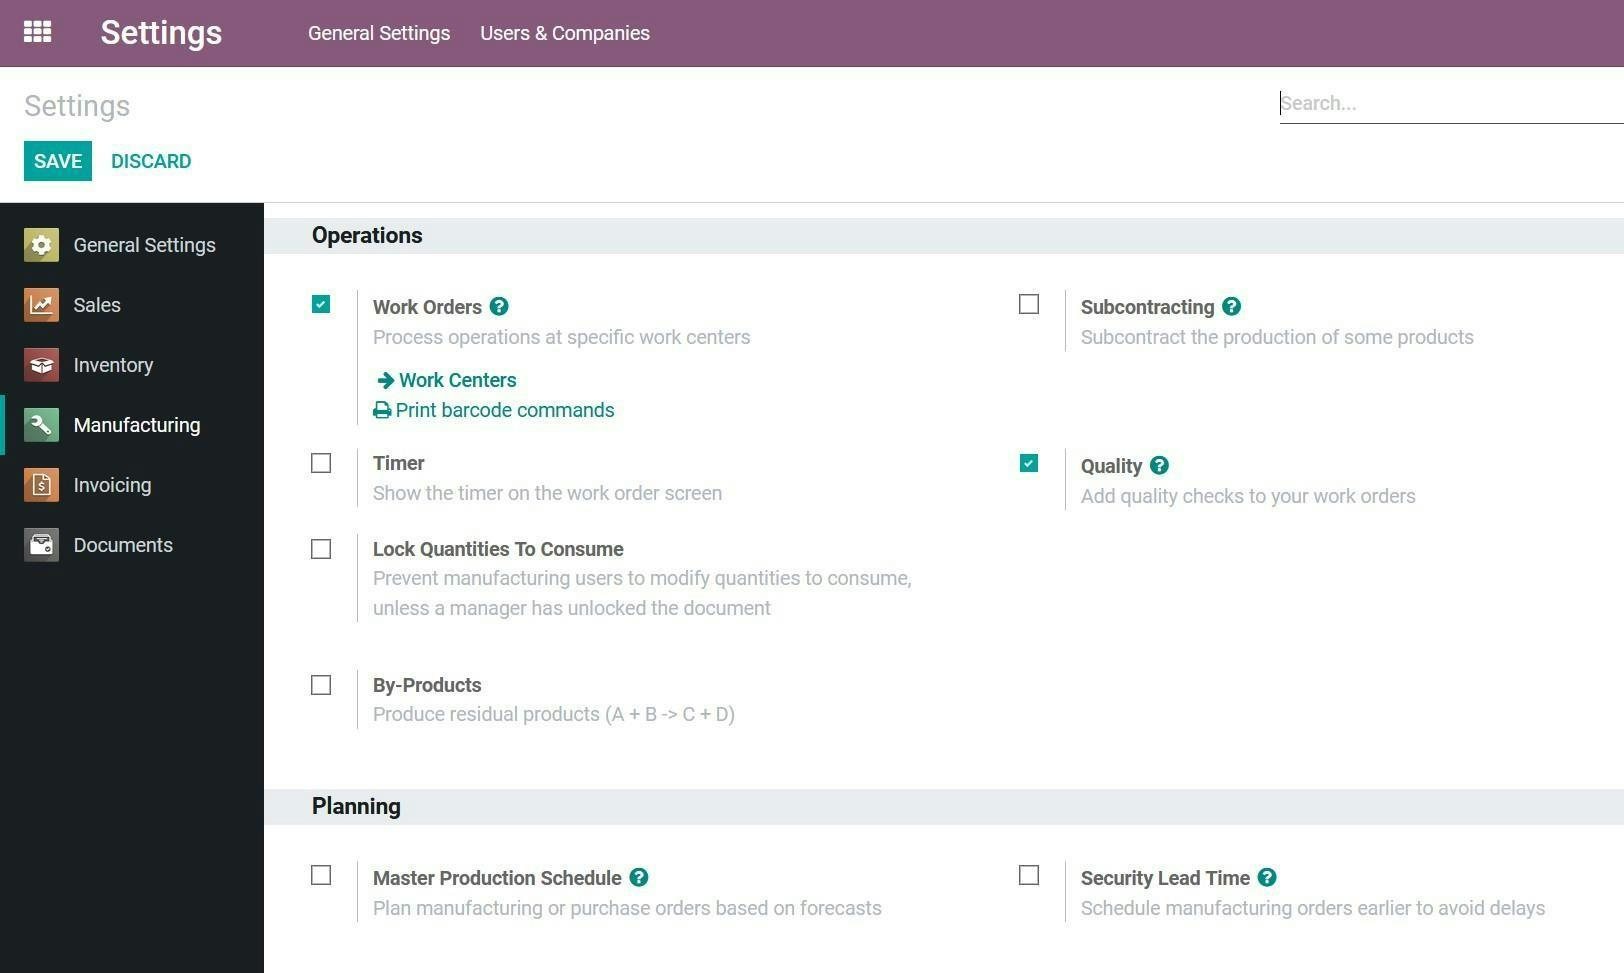
\includegraphics[width=438.64pt,height=262.7pt]{latexImage_2b042cabcb3a41fd9fa70c6eeac7bd1b.png}}
\end{picture}
\newpage
\begin{tikzpicture}[overlay]\path(0pt,0pt);\end{tikzpicture}
\begin{picture}(-5,0)(2.5,0)
\put(500.26,-727.616){\fontsize{12}{1}\usefont{T1}{ptm}{m}{n}\selectfont\color{color_29791}37}
\put(511.78,-727.616){\fontsize{12}{1}\usefont{T1}{ptm}{m}{n}\selectfont\color{color_29791} }
\put(63.024,-726.896){\fontsize{9.96}{1}\usefont{T1}{ptm}{m}{n}\selectfont\color{color_29791} }
\put(512.74,-445.35){\fontsize{9.96}{1}\usefont{T1}{ptm}{m}{n}\selectfont\color{color_29791} }
\put(243.29,-460.71){\fontsize{12}{1}\usefont{T1}{ptm}{b}{n}\selectfont\color{color_29791}圖}
\put(255.29,-460.71){\fontsize{12}{1}\usefont{T1}{ptm}{b}{n}\selectfont\color{color_29791}29}
\put(267.29,-460.71){\fontsize{12}{1}\usefont{T1}{ptm}{b}{n}\selectfont\color{color_29791}用戶介面截圖}
\put(338.71,-460.71){\fontsize{12}{1}\usefont{T1}{ptm}{b}{n}\selectfont\color{color_29791} }
\put(70.05,-444.59){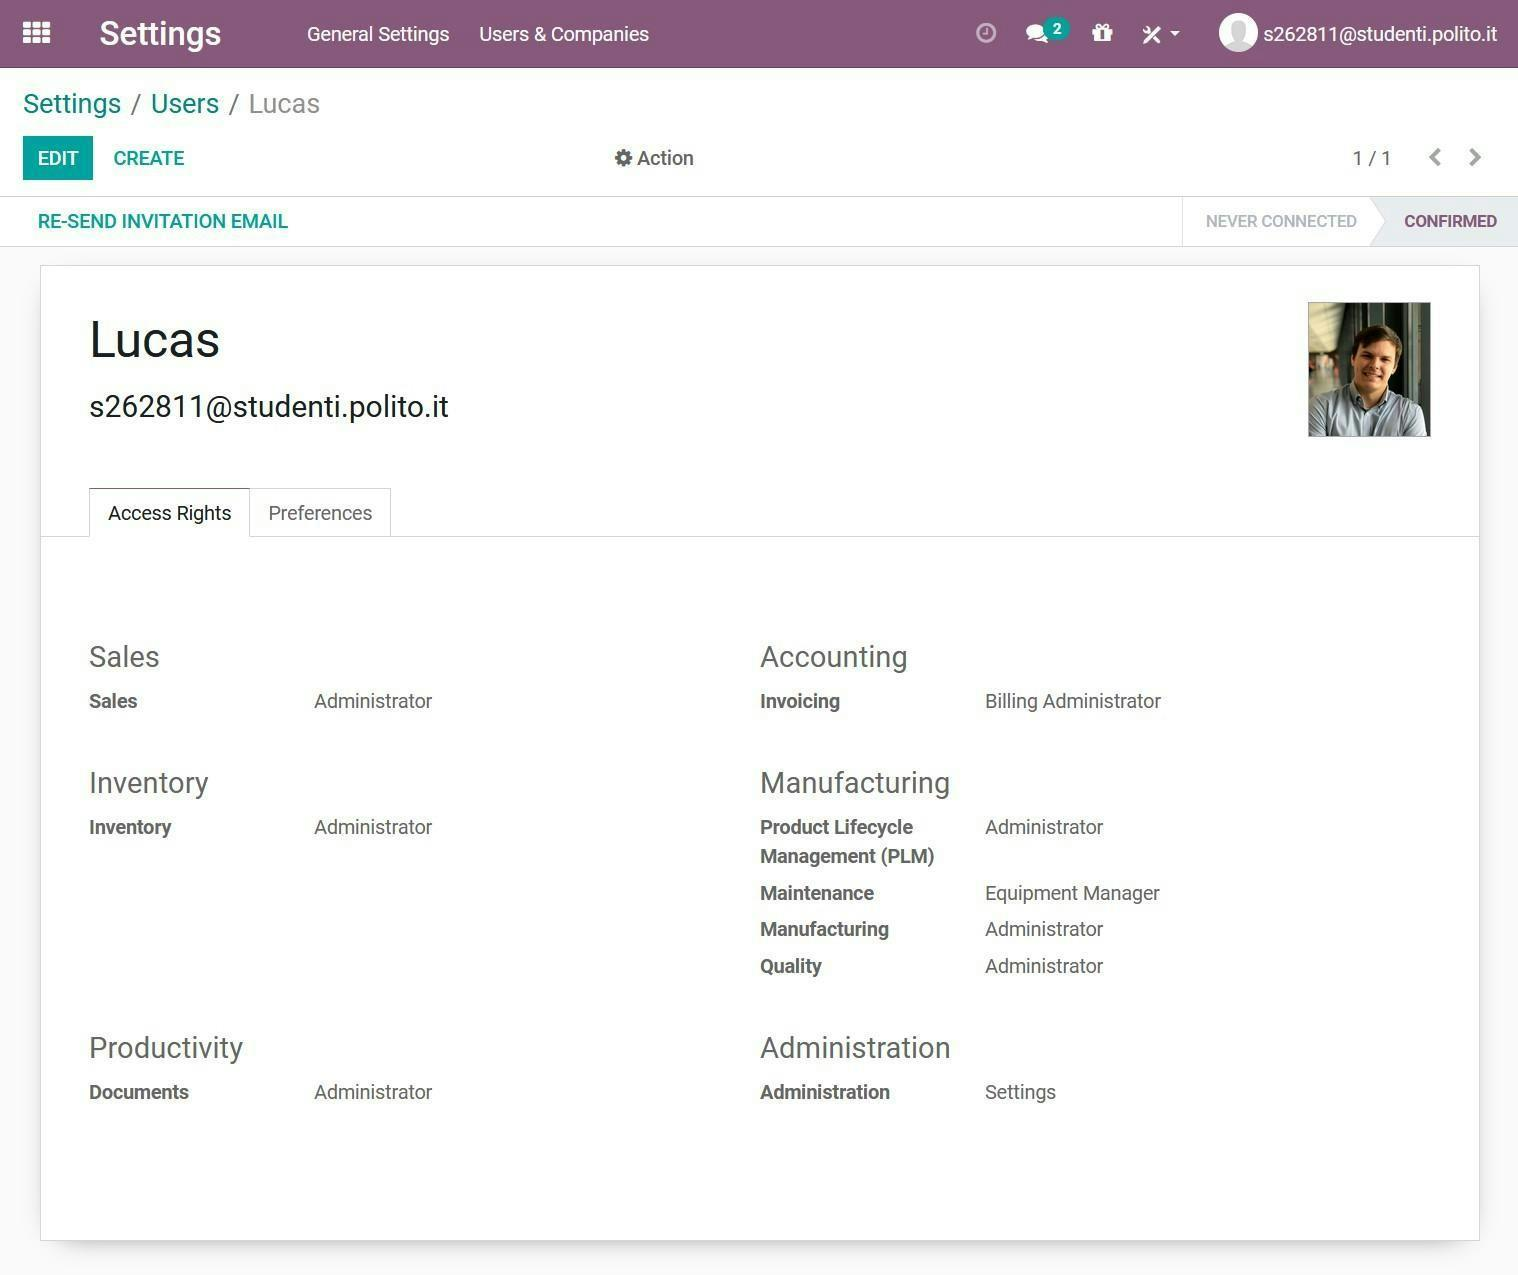
\includegraphics[width=441.88pt,height=370.59pt]{latexImage_f3991b427083fc926885f7f8808abf42.png}}
\put(91.2,-202.07){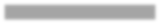
\includegraphics[width=114.95pt,height=16.92pt]{latexImage_c67913f8e34d93bd918ce0f2a51cfd62.png}}
\put(94.12,-197.3499){
\includegraphics[width=109.2pt,height=11.28pt]{latexImage_f237eee757ae1c452b44569bea740bb2.png}}
\put(434.02,-93.22997){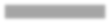
\includegraphics[width=78.597pt,height=16.317pt]{latexImage_ef3c06c5ca02eb104b1283d8c7b4fc17.png}}
\put(437.38,-88.15){
\includegraphics[width=71.997pt,height=9.8397pt]{latexImage_ca03e0ac46b7c604b809da48e4385684.png}}
\end{picture}
\begin{tikzpicture}[overlay]
\path(0pt,0pt);
\end{tikzpicture}
\newpage
\begin{tikzpicture}[overlay]
\path(0pt,0pt);
\draw[color_156960,line width=0.74992pt,line join=round]
(437.73pt, -88.09998pt) -- (509.277pt, -88.09998pt)
 -- (509.277pt, -88.09998pt)
 -- (509.277pt, -78.85016pt)
 -- (509.277pt, -78.85016pt)
 -- (437.73pt, -78.85016pt) -- cycle
;
\begin{scope}
\clip
(497.26pt, -731.216pt) -- (516.1pt, -731.216pt)
 -- (516.1pt, -731.216pt)
 -- (516.1pt, -715.976pt)
 -- (516.1pt, -715.976pt)
 -- (497.26pt, -715.976pt) -- cycle
;
\begin{scope}
\clip
(497.26pt, -731.216pt) -- (516.1pt, -731.216pt)
 -- (516.1pt, -731.216pt)
 -- (516.1pt, -715.976pt)
 -- (516.1pt, -715.976pt)
 -- (497.26pt, -715.976pt) -- cycle
;
\end{scope}
\end{scope}
\end{tikzpicture}
\begin{picture}(-5,0)(2.5,0)
\put(500.26,-727.616){\fontsize{12}{1}\usefont{T1}{ptm}{m}{n}\selectfont\color{color_29791}38}
\put(511.78,-727.616){\fontsize{12}{1}\usefont{T1}{ptm}{m}{n}\selectfont\color{color_29791} }
\put(63.024,-726.896){\fontsize{9.96}{1}\usefont{T1}{ptm}{m}{n}\selectfont\color{color_29791} }
\put(503.02,-348.25){\fontsize{9.96}{1}\usefont{T1}{ptm}{m}{n}\selectfont\color{color_29791} }
\put(217.61,-366.37){\fontsize{12}{1}\usefont{T1}{ptm}{b}{n}\selectfont\color{color_29791}圖}
\put(229.61,-366.37){\fontsize{12}{1}\usefont{T1}{ptm}{b}{n}\selectfont\color{color_29791}30}
\put(241.61,-366.37){\fontsize{12}{1}\usefont{T1}{ptm}{b}{n}\selectfont\color{color_29791} }
\put(244.61,-366.37){\fontsize{12}{1}\usefont{T1}{ptm}{b}{n}\selectfont\color{color_29791}第二個使}
\put(292.49,-366.37){\fontsize{12}{1}\usefont{T1}{ptm}{b}{n}\selectfont\color{color_29791}用者介}
\put(328.37,-366.37){\fontsize{12}{1}\usefont{T1}{ptm}{b}{n}\selectfont\color{color_29791}面}
\put(340.25,-366.37){\fontsize{12}{1}\usefont{T1}{ptm}{b}{n}\selectfont\color{color_29791}截圖}
\put(364.15,-366.37){\fontsize{12}{1}\usefont{T1}{ptm}{b}{n}\selectfont\color{color_29791} }
\put(87.38,-398.29){\fontsize{12}{1}\usefont{T1}{ptm}{m}{n}\selectfont\color{color_29791}很高興指出兩者在訪問許可權上的不同之}
\put(303.41,-398.29){\fontsize{12}{1}\usefont{T1}{ptm}{m}{n}\selectfont\color{color_29791}處}
\put(315.43,-398.29){\fontsize{12}{1}\usefont{T1}{ptm}{m}{n}\selectfont\color{color_29791}。在此示例中,}
\put(399.43,-398.29){\fontsize{12}{1}\usefont{T1}{ptm}{m}{n}\selectfont\color{color_29791}M}
\put(410.11,-398.29){\fontsize{12}{1}\usefont{T1}{ptm}{m}{n}\selectfont\color{color_29791}a}
\put(415.39,-398.29){\fontsize{12}{1}\usefont{T1}{ptm}{m}{n}\selectfont\color{color_29791}r}
\put(419.47,-398.29){\fontsize{12}{1}\usefont{T1}{ptm}{m}{n}\selectfont\color{color_29791}y}
\put(425.47,-398.29){\fontsize{12}{1}\usefont{T1}{ptm}{m}{n}\selectfont\color{color_29791} }
\put(478.66,-398.29){\fontsize{12}{1}\usefont{T1}{ptm}{m}{n}\selectfont\color{color_29791}F}
\put(485.02,-398.29){\fontsize{12}{1}\usefont{T1}{ptm}{m}{n}\selectfont\color{color_29791}i}
\put(488.26,-398.29){\fontsize{12}{1}\usefont{T1}{ptm}{m}{n}\selectfont\color{color_29791}c}
\put(493.42,-398.29){\fontsize{12}{1}\usefont{T1}{ptm}{m}{n}\selectfont\color{color_29791}t}
\put(496.66,-398.29){\fontsize{12}{1}\usefont{T1}{ptm}{m}{n}\selectfont\color{color_29791}i}
\put(499.9,-398.29){\fontsize{12}{1}\usefont{T1}{ptm}{m}{n}\selectfont\color{color_29791}o}
\put(505.78,-398.29){\fontsize{12}{1}\usefont{T1}{ptm}{m}{n}\selectfont\color{color_29791}n}
\put(69.384,-416.19){\fontsize{12}{1}\usefont{T1}{ptm}{m}{n}\selectfont\color{color_29791}是以工程師身份創建的,因此她的大部分許可權都與製造程式有關,而她則被拒絕}
\put(69.384,-434.07){\fontsize{12}{1}\usefont{T1}{ptm}{m}{n}\selectfont\color{color_29791}訪問其他部}
\put(129.38,-434.07){\fontsize{12}{1}\usefont{T1}{ptm}{m}{n}\selectfont\color{color_29791}分}
\put(141.38,-434.07){\fontsize{12}{1}\usefont{T1}{ptm}{m}{n}\selectfont\color{color_29791},例如銷售或會計。}
\put(249.41,-434.07){\fontsize{12}{1}\usefont{T1}{ptm}{m}{n}\selectfont\color{color_29791} }
\put(63.024,-453.15){\fontsize{12}{1}\usefont{T1}{ptm}{m}{n}\selectfont\color{color_29791} }
\put(105.38,-473.19){\fontsize{12.81913}{1}\usefont{T1}{ptm}{b}{n}\selectfont\color{color_29791}5.}
\put(114.9648,-473.19){\fontsize{12.81913}{1}\usefont{T1}{ptm}{b}{n}\selectfont\color{color_29791}3}
\put(121.4307,-473.19){\fontsize{12.81913}{1}\usefont{T1}{ptm}{b}{n}\selectfont\color{color_29791}.}
\put(124.5495,-473.19){\fontsize{12.81913}{1}\usefont{T1}{ptm}{b}{n}\selectfont\color{color_29791}2}
\put(131.0154,-473.19){\fontsize{12.81913}{1}\usefont{T1}{ptm}{b}{n}\selectfont\color{color_29791}.}
\put(134.3,-473.19){\fontsize{12.83539}{1}\usefont{T1}{ptm}{b}{n}\selectfont\color{color_29791} }
\put(137.66,-473.19){\fontsize{12.96}{1}\usefont{T1}{ptm}{b}{n}\selectfont\color{color_29791}工}
\put(150.3738,-473.19){\fontsize{12.96}{1}\usefont{T1}{ptm}{b}{n}\selectfont\color{color_29791}作}
\put(163.2171,-473.19){\fontsize{12.96}{1}\usefont{T1}{ptm}{b}{n}\selectfont\color{color_29791}中}
\put(176.0605,-473.19){\fontsize{12.96}{1}\usefont{T1}{ptm}{b}{n}\selectfont\color{color_29791}心}
\put(188.7742,-473.19){\fontsize{12.96}{1}\usefont{T1}{ptm}{b}{n}\selectfont\color{color_29791}和}
\put(201.6176,-473.19){\fontsize{12.96}{1}\usefont{T1}{ptm}{b}{n}\selectfont\color{color_29791}設}
\put(214.4609,-473.19){\fontsize{12.96}{1}\usefont{T1}{ptm}{b}{n}\selectfont\color{color_29791}備}
\put(227.33,-473.19){\fontsize{12.96}{1}\usefont{T1}{ptm}{b}{n}\selectfont\color{color_29791} }
\put(82.944,-501.63){\fontsize{12}{1}\usefont{T1}{ptm}{m}{n}\selectfont\color{color_29791}工作中心在}
\put(142.34,-501.63){\fontsize{12}{1}\usefont{T1}{ptm}{m}{n}\selectfont\color{color_29791}O}
\put(150.86,-501.63){\fontsize{12}{1}\usefont{T1}{ptm}{m}{n}\selectfont\color{color_29791}do}
\put(162.74,-501.63){\fontsize{12}{1}\usefont{T1}{ptm}{m}{n}\selectfont\color{color_29791}o}
\put(168.62,-501.63){\fontsize{12}{1}\usefont{T1}{ptm}{m}{n}\selectfont\color{color_29791}中}
\put(180.5,-501.63){\fontsize{12}{1}\usefont{T1}{ptm}{m}{n}\selectfont\color{color_29791}非}
\put(192.38,-501.63){\fontsize{12}{1}\usefont{T1}{ptm}{m}{n}\selectfont\color{color_29791}常靈}
\put(216.26,-501.63){\fontsize{12}{1}\usefont{T1}{ptm}{m}{n}\selectfont\color{color_29791}活}
\put(228.14,-501.63){\fontsize{12}{1}\usefont{T1}{ptm}{m}{n}\selectfont\color{color_29791},}
\put(240.02,-501.63){\fontsize{12}{1}\usefont{T1}{ptm}{m}{n}\selectfont\color{color_29791}可}
\put(251.9,-501.63){\fontsize{12}{1}\usefont{T1}{ptm}{m}{n}\selectfont\color{color_29791}以}
\put(263.78,-501.63){\fontsize{12}{1}\usefont{T1}{ptm}{m}{n}\selectfont\color{color_29791}根}
\put(275.66,-501.63){\fontsize{12}{1}\usefont{T1}{ptm}{m}{n}\selectfont\color{color_29791}據}
\put(287.54,-501.63){\fontsize{12}{1}\usefont{T1}{ptm}{m}{n}\selectfont\color{color_29791}需要}
\put(311.42,-501.63){\fontsize{12}{1}\usefont{T1}{ptm}{m}{n}\selectfont\color{color_29791}進行}
\put(335.3,-501.63){\fontsize{12}{1}\usefont{T1}{ptm}{m}{n}\selectfont\color{color_29791}更}
\put(347.1801,-501.63){\fontsize{12}{1}\usefont{T1}{ptm}{m}{n}\selectfont\color{color_29791}改}
\put(359.0601,-501.63){\fontsize{12}{1}\usefont{T1}{ptm}{m}{n}\selectfont\color{color_29791}和}
\put(370.9401,-501.63){\fontsize{12}{1}\usefont{T1}{ptm}{m}{n}\selectfont\color{color_29791}擴}
\put(382.8201,-501.63){\fontsize{12}{1}\usefont{T1}{ptm}{m}{n}\selectfont\color{color_29791}展}
\put(394.7001,-501.63){\fontsize{12}{1}\usefont{T1}{ptm}{m}{n}\selectfont\color{color_29791}。}
\put(406.5801,-501.63){\fontsize{12}{1}\usefont{T1}{ptm}{m}{n}\selectfont\color{color_29791}可以}
\put(430.4601,-501.63){\fontsize{12}{1}\usefont{T1}{ptm}{m}{n}\selectfont\color{color_29791}在創}
\put(454.3401,-501.63){\fontsize{12}{1}\usefont{T1}{ptm}{m}{n}\selectfont\color{color_29791}建}
\put(466.2201,-501.63){\fontsize{12}{1}\usefont{T1}{ptm}{m}{n}\selectfont\color{color_29791}產}
\put(478.1001,-501.63){\fontsize{12}{1}\usefont{T1}{ptm}{m}{n}\selectfont\color{color_29791}品}
\put(489.9801,-501.63){\fontsize{12}{1}\usefont{T1}{ptm}{m}{n}\selectfont\color{color_29791}專}
\put(69.384,-519.51){\fontsize{12}{1}\usefont{T1}{ptm}{m}{n}\selectfont\color{color_29791}案后創建工作中心}
\put(164.532,-519.51){\fontsize{12}{1}\usefont{T1}{ptm}{m}{n}\selectfont\color{color_29791},以}
\put(188.4,-519.51){\fontsize{12}{1}\usefont{T1}{ptm}{m}{n}\selectfont\color{color_29791}便在您對產品最終}
\put(283.548,-519.51){\fontsize{12}{1}\usefont{T1}{ptm}{m}{n}\selectfont\color{color_29791}將是}
\put(307.416,-519.51){\fontsize{12}{1}\usefont{T1}{ptm}{m}{n}\selectfont\color{color_29791}什麼有所瞭解后對}
\put(402.564,-519.51){\fontsize{12}{1}\usefont{T1}{ptm}{m}{n}\selectfont\color{color_29791}車間}
\put(426.432,-519.51){\fontsize{12}{1}\usefont{T1}{ptm}{m}{n}\selectfont\color{color_29791}進行重組。然}
\put(69.384,-537.39){\fontsize{12}{1}\usefont{T1}{ptm}{m}{n}\selectfont\color{color_29791}而,對於大多數情}
\put(164.532,-537.39){\fontsize{12}{1}\usefont{T1}{ptm}{m}{n}\selectfont\color{color_29791}況來}
\put(188.4,-537.39){\fontsize{12}{1}\usefont{T1}{ptm}{m}{n}\selectfont\color{color_29791}說,這似乎是不現}
\put(283.548,-537.39){\fontsize{12}{1}\usefont{T1}{ptm}{m}{n}\selectfont\color{color_29791}實的}
\put(307.416,-537.39){\fontsize{12}{1}\usefont{T1}{ptm}{m}{n}\selectfont\color{color_29791},因為工作中心在}
\put(402.564,-537.39){\fontsize{12}{1}\usefont{T1}{ptm}{m}{n}\selectfont\color{color_29791}現實}
\put(426.432,-537.39){\fontsize{12}{1}\usefont{T1}{ptm}{m}{n}\selectfont\color{color_29791}世界中是更嚴}
\put(69.384,-555.27){\fontsize{12}{1}\usefont{T1}{ptm}{m}{n}\selectfont\color{color_29791}格的結構}
\put(116.9,-555.27){\fontsize{12}{1}\usefont{T1}{ptm}{m}{n}\selectfont\color{color_29791}——}
\put(140.66,-555.27){\fontsize{12}{1}\usefont{T1}{ptm}{m}{n}\selectfont\color{color_29791}它}
\put(152.54,-555.27){\fontsize{12}{1}\usefont{T1}{ptm}{m}{n}\selectfont\color{color_29791}們的}
\put(176.42,-555.27){\fontsize{12}{1}\usefont{T1}{ptm}{m}{n}\selectfont\color{color_29791}變化}
\put(200.3,-555.27){\fontsize{12}{1}\usefont{T1}{ptm}{m}{n}\selectfont\color{color_29791}不}
\put(212.18,-555.27){\fontsize{12}{1}\usefont{T1}{ptm}{m}{n}\selectfont\color{color_29791}如}
\put(224.06,-555.27){\fontsize{12}{1}\usefont{T1}{ptm}{m}{n}\selectfont\color{color_29791}產}
\put(235.94,-555.27){\fontsize{12}{1}\usefont{T1}{ptm}{m}{n}\selectfont\color{color_29791}品}
\put(247.82,-555.27){\fontsize{12}{1}\usefont{T1}{ptm}{m}{n}\selectfont\color{color_29791},}
\put(259.7,-555.27){\fontsize{12}{1}\usefont{T1}{ptm}{m}{n}\selectfont\color{color_29791}因}
\put(271.58,-555.27){\fontsize{12}{1}\usefont{T1}{ptm}{m}{n}\selectfont\color{color_29791}為它}
\put(295.4601,-555.27){\fontsize{12}{1}\usefont{T1}{ptm}{m}{n}\selectfont\color{color_29791}們往}
\put(319.3401,-555.27){\fontsize{12}{1}\usefont{T1}{ptm}{m}{n}\selectfont\color{color_29791}往}
\put(331.2201,-555.27){\fontsize{12}{1}\usefont{T1}{ptm}{m}{n}\selectfont\color{color_29791}容}
\put(343.1001,-555.27){\fontsize{12}{1}\usefont{T1}{ptm}{m}{n}\selectfont\color{color_29791}納}
\put(354.9801,-555.27){\fontsize{12}{1}\usefont{T1}{ptm}{m}{n}\selectfont\color{color_29791}重}
\put(366.8601,-555.27){\fontsize{12}{1}\usefont{T1}{ptm}{m}{n}\selectfont\color{color_29791}型}
\put(378.7401,-555.27){\fontsize{12}{1}\usefont{T1}{ptm}{m}{n}\selectfont\color{color_29791}機}
\put(390.6201,-555.27){\fontsize{12}{1}\usefont{T1}{ptm}{m}{n}\selectfont\color{color_29791}械。}
\put(414.67,-555.27){\fontsize{12}{1}\usefont{T1}{ptm}{m}{n}\selectfont\color{color_29791} }
\put(82.944,-588.06){\fontsize{12}{1}\usefont{T1}{ptm}{m}{n}\selectfont\color{color_29791}在這個類比中,我}
\put(178.092,-588.06){\fontsize{12}{1}\usefont{T1}{ptm}{m}{n}\selectfont\color{color_29791}們認}
\put(201.96,-588.06){\fontsize{12}{1}\usefont{T1}{ptm}{m}{n}\selectfont\color{color_29791}為該公司從一開始}
\put(297.108,-588.06){\fontsize{12}{1}\usefont{T1}{ptm}{m}{n}\selectfont\color{color_29791}就已}
\put(320.976,-588.06){\fontsize{12}{1}\usefont{T1}{ptm}{m}{n}\selectfont\color{color_29791}經}
\put(332.95,-588.06){\fontsize{12}{1}\usefont{T1}{ptm}{m}{n}\selectfont\color{color_29791}有}
\put(344.47,-588.06){\fontsize{12}{1}\usefont{T1}{ptm}{m}{n}\selectfont\color{color_29791} }
\put(506.98,-588.06){\fontsize{12}{1}\usefont{T1}{ptm}{m}{n}\selectfont\color{color_29791}3}
\put(512.5,-588.06){\fontsize{12}{1}\usefont{T1}{ptm}{m}{n}\selectfont\color{color_29791} }
\put(69.384,-605.94){\fontsize{12}{1}\usefont{T1}{ptm}{m}{n}\selectfont\color{color_29791}個工作中心,因此}
\put(164.532,-605.94){\fontsize{12}{1}\usefont{T1}{ptm}{m}{n}\selectfont\color{color_29791}工作}
\put(188.4,-605.94){\fontsize{12}{1}\usefont{T1}{ptm}{m}{n}\selectfont\color{color_29791}中心和機器是事先}
\put(283.548,-605.94){\fontsize{12}{1}\usefont{T1}{ptm}{m}{n}\selectfont\color{color_29791}創建}
\put(307.416,-605.94){\fontsize{12}{1}\usefont{T1}{ptm}{m}{n}\selectfont\color{color_29791}的。這對於有興趣}
\put(402.564,-605.94){\fontsize{12}{1}\usefont{T1}{ptm}{m}{n}\selectfont\color{color_29791}實現}
\put(426.55,-605.94){\fontsize{12}{1}\usefont{T1}{ptm}{m}{n}\selectfont\color{color_29791}O}
\put(435.07,-605.94){\fontsize{12}{1}\usefont{T1}{ptm}{m}{n}\selectfont\color{color_29791}d}
\put(440.95,-605.94){\fontsize{12}{1}\usefont{T1}{ptm}{m}{n}\selectfont\color{color_29791}o}
\put(446.83,-605.94){\fontsize{12}{1}\usefont{T1}{ptm}{m}{n}\selectfont\color{color_29791}o}
\put(452.74,-605.94){\fontsize{12}{1}\usefont{T1}{ptm}{m}{n}\selectfont\color{color_29791}並}
\put(464.62,-605.94){\fontsize{12}{1}\usefont{T1}{ptm}{m}{n}\selectfont\color{color_29791}節}
\put(476.5,-605.94){\fontsize{12}{1}\usefont{T1}{ptm}{m}{n}\selectfont\color{color_29791}省一}
\put(69.384,-623.94){\fontsize{12}{1}\usefont{T1}{ptm}{m}{n}\selectfont\color{color_29791}些時間的讀者來說}
\put(164.532,-623.94){\fontsize{12}{1}\usefont{T1}{ptm}{m}{n}\selectfont\color{color_29791}更有}
\put(188.4,-623.94){\fontsize{12}{1}\usefont{T1}{ptm}{m}{n}\selectfont\color{color_29791}用。}
\put(212.21,-623.94){\fontsize{12}{1}\usefont{T1}{ptm}{m}{n}\selectfont\color{color_29791} }
\put(82.944,-656.58){\fontsize{12}{1}\usefont{T1}{ptm}{m}{n}\selectfont\color{color_29791}我們從}
\put(118.824,-656.58){\fontsize{12}{1}\usefont{T1}{ptm}{m}{n}\selectfont\color{color_29791}創建我}
\put(154.704,-656.58){\fontsize{12}{1}\usefont{T1}{ptm}{m}{n}\selectfont\color{color_29791}們擁}
\put(178.584,-656.58){\fontsize{12}{1}\usefont{T1}{ptm}{m}{n}\selectfont\color{color_29791}有的}
\put(202.464,-656.58){\fontsize{12}{1}\usefont{T1}{ptm}{m}{n}\selectfont\color{color_29791}設備開}
\put(238.344,-656.58){\fontsize{12}{1}\usefont{T1}{ptm}{m}{n}\selectfont\color{color_29791}始。這}
\put(274.224,-656.58){\fontsize{12}{1}\usefont{T1}{ptm}{m}{n}\selectfont\color{color_29791}是維}
\put(298.104,-656.58){\fontsize{12}{1}\usefont{T1}{ptm}{m}{n}\selectfont\color{color_29791}護組}
\put(321.984,-656.58){\fontsize{12}{1}\usefont{T1}{ptm}{m}{n}\selectfont\color{color_29791}織中強}
\put(357.864,-656.58){\fontsize{12}{1}\usefont{T1}{ptm}{m}{n}\selectfont\color{color_29791}調的項}
\put(393.744,-656.58){\fontsize{12}{1}\usefont{T1}{ptm}{m}{n}\selectfont\color{color_29791}類。}
\put(417.6241,-656.58){\fontsize{12}{1}\usefont{T1}{ptm}{m}{n}\selectfont\color{color_29791}負責}
\put(441.5041,-656.58){\fontsize{12}{1}\usefont{T1}{ptm}{m}{n}\selectfont\color{color_29791}管理設}
\put(477.3841,-656.58){\fontsize{12}{1}\usefont{T1}{ptm}{m}{n}\selectfont\color{color_29791}備的}
\put(501.34,-656.58){\fontsize{12}{1}\usefont{T1}{ptm}{m}{n}\selectfont\color{color_29791} }
\put(69.384,-674.58){\fontsize{12}{1}\usefont{T1}{ptm}{m}{n}\selectfont\color{color_29791}應用程式是維護應用程式。下圖是}
\put(249.41,-674.58){\fontsize{12}{1}\usefont{T1}{ptm}{m}{n}\selectfont\color{color_29791}Odoo}
\put(276.05,-674.58){\fontsize{12}{1}\usefont{T1}{ptm}{m}{n}\selectfont\color{color_29791}如何描繪}
\put(324.07,-674.58){\fontsize{12}{1}\usefont{T1}{ptm}{m}{n}\selectfont\color{color_29791}3D}
\put(338.71,-674.58){\fontsize{12}{1}\usefont{T1}{ptm}{m}{n}\selectfont\color{color_29791}印表機設備專案的示例(圖}
\put(482.74,-674.58){\fontsize{12}{1}\usefont{T1}{ptm}{m}{n}\selectfont\color{color_29791}31}
\put(494.74,-674.58){\fontsize{12}{1}\usefont{T1}{ptm}{m}{n}\selectfont\color{color_29791})}
\put(506.74,-674.58){\fontsize{12}{1}\usefont{T1}{ptm}{m}{n}\selectfont\color{color_29791}。}
\put(518.26,-674.58){\fontsize{12}{1}\usefont{T1}{ptm}{m}{n}\selectfont\color{color_29791} }
\put(73.3,-348.25){
\includegraphics[width=429.62pt,height=287.25pt]{latexImage_3083b45acd47366d678f93caeb1272c1.png}}
\end{picture}
\newpage
\begin{tikzpicture}[overlay]\path(0pt,0pt);\end{tikzpicture}
\begin{picture}(-5,0)(2.5,0)
\put(500.26,-727.616){\fontsize{12}{1}\usefont{T1}{ptm}{m}{n}\selectfont\color{color_29791}39}
\put(511.78,-727.616){\fontsize{12}{1}\usefont{T1}{ptm}{m}{n}\selectfont\color{color_29791} }
\put(63.024,-726.896){\fontsize{9.96}{1}\usefont{T1}{ptm}{m}{n}\selectfont\color{color_29791} }
\put(73.75,-577){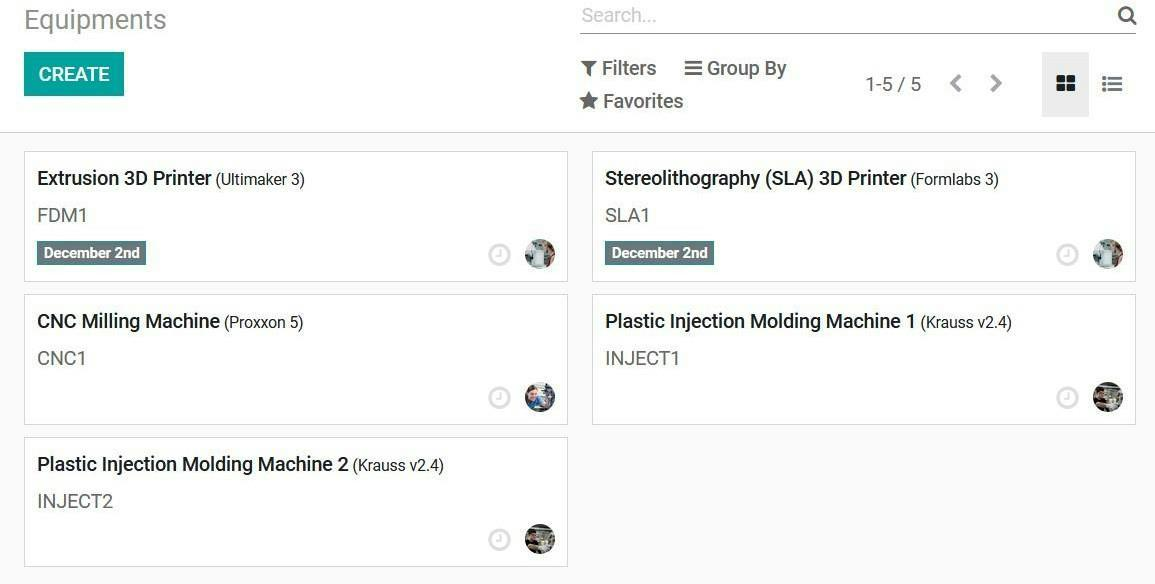
\includegraphics[width=434.75pt,height=219pt]{latexImage_79a7fa40060fc47d1d03b35492d8972c.png}}
\put(506.5,-281.77){\fontsize{9.96}{1}\usefont{T1}{ptm}{m}{n}\selectfont\color{color_29791} }
\put(214.49,-299.17){\fontsize{12}{1}\usefont{T1}{ptm}{b}{n}\selectfont\color{color_29791}圖}
\put(226.49,-299.17){\fontsize{12}{1}\usefont{T1}{ptm}{b}{n}\selectfont\color{color_29791}31}
\put(238.49,-299.17){\fontsize{12}{1}\usefont{T1}{ptm}{b}{n}\selectfont\color{color_29791} }
\put(241.25,-299.17){\fontsize{12}{1}\usefont{T1}{ptm}{b}{n}\selectfont\color{color_29791}Od}
\put(257.318,-299.17){\fontsize{12}{1}\usefont{T1}{ptm}{b}{n}\selectfont\color{color_29791}oo3D}
\put(283.97,-299.17){\fontsize{12}{1}\usefont{T1}{ptm}{b}{n}\selectfont\color{color_29791}印}
\put(295.85,-299.17){\fontsize{12}{1}\usefont{T1}{ptm}{b}{n}\selectfont\color{color_29791}表}
\put(307.73,-299.17){\fontsize{12}{1}\usefont{T1}{ptm}{b}{n}\selectfont\color{color_29791}機}
\put(319.61,-299.17){\fontsize{12}{1}\usefont{T1}{ptm}{b}{n}\selectfont\color{color_29791}設備}
\put(343.49,-299.17){\fontsize{12}{1}\usefont{T1}{ptm}{b}{n}\selectfont\color{color_29791}專}
\put(355.37,-299.17){\fontsize{12}{1}\usefont{T1}{ptm}{b}{n}\selectfont\color{color_29791}案}
\put(367.39,-299.17){\fontsize{12}{1}\usefont{T1}{ptm}{b}{n}\selectfont\color{color_29791} }
\put(82.944,-331.21){\fontsize{12}{1}\usefont{T1}{ptm}{m}{n}\selectfont\color{color_29791}除了這台}
\put(130.1,-331.21){\fontsize{12}{1}\usefont{T1}{ptm}{m}{n}\selectfont\color{color_29791} }
\put(135.86,-331.21){\fontsize{12}{1}\usefont{T1}{ptm}{m}{n}\selectfont\color{color_29791}3D}
\put(150.5,-331.21){\fontsize{12}{1}\usefont{T1}{ptm}{m}{n}\selectfont\color{color_29791} }
\put(155.66,-331.21){\fontsize{12}{1}\usefont{T1}{ptm}{m}{n}\selectfont\color{color_29791}印表機之外,還創建了以下設備,用於整個開發}
\put(407.71,-331.21){\fontsize{12}{1}\usefont{T1}{ptm}{m}{n}\selectfont\color{color_29791}/}
\put(411.07,-331.21){\fontsize{12}{1}\usefont{T1}{ptm}{m}{n}\selectfont\color{color_29791}生產過程(}
\put(471.1,-331.21){\fontsize{12}{1}\usefont{T1}{ptm}{m}{n}\selectfont\color{color_29791}圖}
\put(482.62,-331.21){\fontsize{12}{1}\usefont{T1}{ptm}{m}{n}\selectfont\color{color_29791} }
\put(488.14,-331.21){\fontsize{12}{1}\usefont{T1}{ptm}{m}{n}\selectfont\color{color_29791}32}
\put(499.78,-331.21){\fontsize{12}{1}\usefont{T1}{ptm}{m}{n}\selectfont\color{color_29791}):}
\put(523.42,-331.21){\fontsize{12}{1}\usefont{T1}{ptm}{m}{n}\selectfont\color{color_29791} }
\put(63.024,-354.13){\fontsize{9.96}{1}\usefont{T1}{ptm}{m}{n}\selectfont\color{color_29791} }
\put(243.41,-593.46){\fontsize{12}{1}\usefont{T1}{ptm}{b}{n}\selectfont\color{color_29791}圖}
\put(255.41,-593.46){\fontsize{12}{1}\usefont{T1}{ptm}{b}{n}\selectfont\color{color_29791}32}
\put(267.41,-593.46){\fontsize{12}{1}\usefont{T1}{ptm}{b}{n}\selectfont\color{color_29791}設備專案概覽}
\put(338.83,-593.46){\fontsize{12}{1}\usefont{T1}{ptm}{b}{n}\selectfont\color{color_29791} }
\put(82.944,-625.26){\fontsize{12}{1}\usefont{T1}{ptm}{m}{n}\selectfont\color{color_29791}這就是有}
\put(130.94,-625.26){\fontsize{12}{1}\usefont{T1}{ptm}{m}{n}\selectfont\color{color_29791}關}
\put(142.46,-625.26){\fontsize{12}{1}\usefont{T1}{ptm}{m}{n}\selectfont\color{color_29791} }
\put(487.9,-625.26){\fontsize{12}{1}\usefont{T1}{ptm}{m}{n}\selectfont\color{color_29791}P}
\put(494.38,-625.26){\fontsize{12}{1}\usefont{T1}{ptm}{m}{n}\selectfont\color{color_29791}L}
\put(501.46,-625.26){\fontsize{12}{1}\usefont{T1}{ptm}{m}{n}\selectfont\color{color_29791}M}
\put(511.78,-625.26){\fontsize{12}{1}\usefont{T1}{ptm}{m}{n}\selectfont\color{color_29791} }
\put(69.384,-643.14){\fontsize{12}{1}\usefont{T1}{ptm}{m}{n}\selectfont\color{color_29791}的軟體限制開始顯}
\put(164.532,-643.14){\fontsize{12}{1}\usefont{T1}{ptm}{m}{n}\selectfont\color{color_29791}現的}
\put(188.4,-643.14){\fontsize{12}{1}\usefont{T1}{ptm}{m}{n}\selectfont\color{color_29791}地方。儘管設備專}
\put(283.548,-643.14){\fontsize{12}{1}\usefont{T1}{ptm}{m}{n}\selectfont\color{color_29791}案允}
\put(307.416,-643.14){\fontsize{12}{1}\usefont{T1}{ptm}{m}{n}\selectfont\color{color_29791}許您使用某種級別}
\put(402.564,-643.14){\fontsize{12}{1}\usefont{T1}{ptm}{m}{n}\selectfont\color{color_29791}的元}
\put(426.432,-643.14){\fontsize{12}{1}\usefont{T1}{ptm}{m}{n}\selectfont\color{color_29791}數據(描述文}
\put(69.384,-661.02){\fontsize{12}{1}\usefont{T1}{ptm}{m}{n}\selectfont\color{color_29791}本、負責使用者、}
\put(164.532,-661.02){\fontsize{12}{1}\usefont{T1}{ptm}{m}{n}\selectfont\color{color_29791}維護}
\put(188.4,-661.02){\fontsize{12}{1}\usefont{T1}{ptm}{m}{n}\selectfont\color{color_29791}數據和供應商)}
\put(271.61,-661.02){\fontsize{12}{1}\usefont{T1}{ptm}{m}{n}\selectfont\color{color_29791}。它不允許上傳任何}
\put(378.41,-661.02){\fontsize{12}{1}\usefont{T1}{ptm}{m}{n}\selectfont\color{color_29791}類型的檔}
\put(425.81,-661.02){\fontsize{12}{1}\usefont{T1}{ptm}{m}{n}\selectfont\color{color_29791}附加到專案類}
\put(497.02,-661.02){\fontsize{12}{1}\usefont{T1}{ptm}{m}{n}\selectfont\color{color_29791} }
\put(69.384,-678.9){\fontsize{12}{1}\usefont{T1}{ptm}{m}{n}\selectfont\color{color_29791}(機器手冊、報告等)。這是一個很大的弱點,因為檔管理是人們一致認為是}
\put(477.46,-678.9){\fontsize{15}{1}\usefont{T1}{ptm}{m}{n}\selectfont\color{color_29791} }
\put(487.9,-678.9){\fontsize{12}{1}\usefont{T1}{ptm}{m}{n}\selectfont\color{color_29791}P}
\put(494.38,-678.9){\fontsize{12}{1}\usefont{T1}{ptm}{m}{n}\selectfont\color{color_29791}L}
\put(501.46,-678.9){\fontsize{12}{1}\usefont{T1}{ptm}{m}{n}\selectfont\color{color_29791}M}
\put(511.78,-678.9){\fontsize{12}{1}\usefont{T1}{ptm}{m}{n}\selectfont\color{color_29791} }
\put(73.75,-281.75){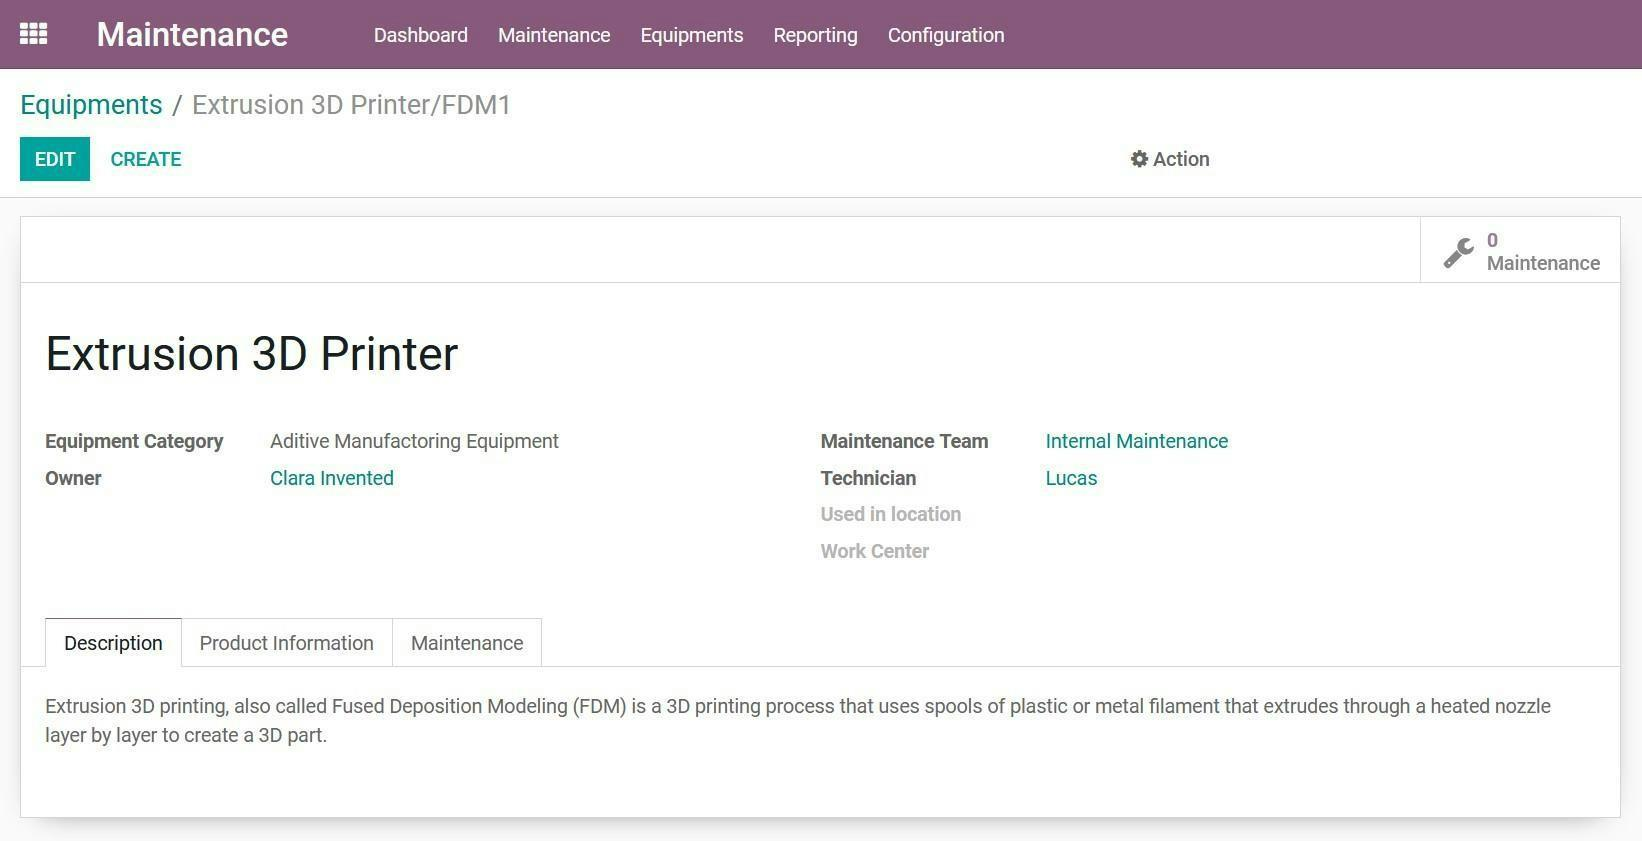
\includegraphics[width=432.65pt,height=220.75pt]{latexImage_6a2e50a51213c2c7c3cb83b88726e23d.png}}
\end{picture}
\newpage
\begin{tikzpicture}[overlay]\path(0pt,0pt);\end{tikzpicture}
\begin{picture}(-5,0)(2.5,0)
\put(500.26,-727.616){\fontsize{12}{1}\usefont{T1}{ptm}{m}{n}\selectfont\color{color_29791}40}
\put(511.78,-727.616){\fontsize{12}{1}\usefont{T1}{ptm}{m}{n}\selectfont\color{color_29791} }
\put(63.024,-726.896){\fontsize{9.96}{1}\usefont{T1}{ptm}{m}{n}\selectfont\color{color_29791} }
\put(70.05,-599.91){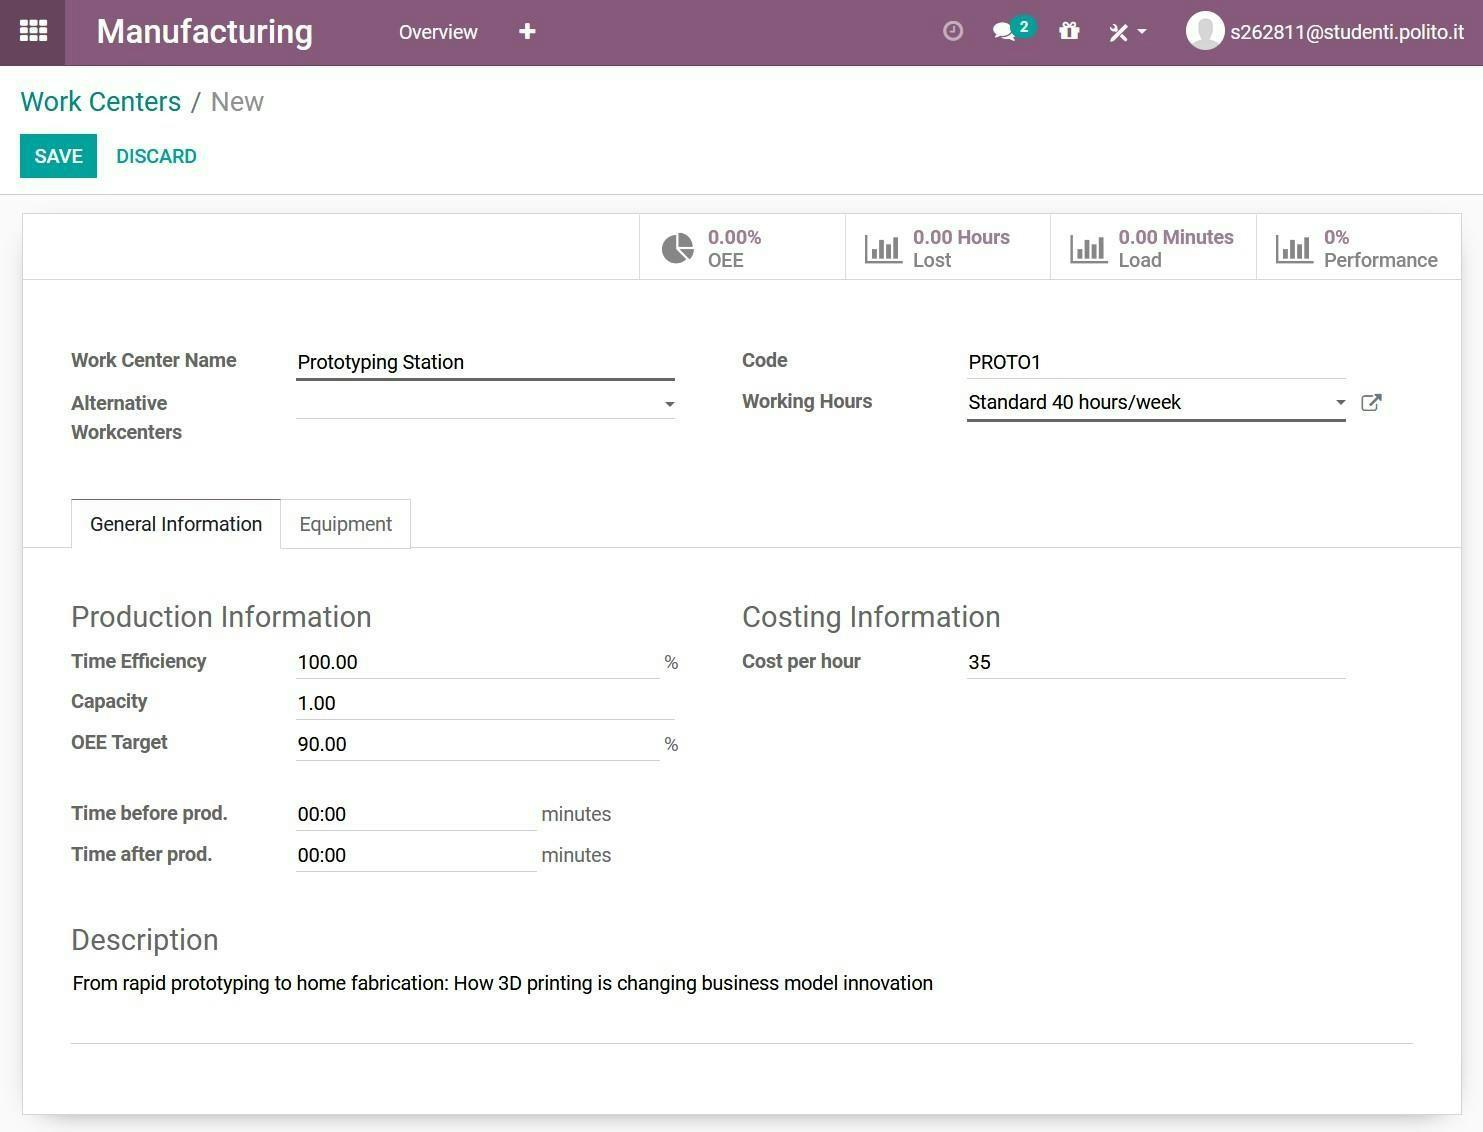
\includegraphics[width=441.88pt,height=337.26pt]{latexImage_dffed640250f71b6f3849b5a37a36e39.png}}
\put(433.06,-281.88){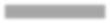
\includegraphics[width=78.717pt,height=16.315pt]{latexImage_735cf46d81e0b7a65bc293b697365e45.png}}
\put(436.34,-276.72){
\includegraphics[width=72.237pt,height=9.5986pt]{latexImage_3cf4706486a807110f99227f5f242d08.png}}
\end{picture}
\begin{tikzpicture}[overlay]
\path(0pt,0pt);
\draw[color_156960,line width=0.75pt,line join=round]
(436.83pt, -276.75pt) -- (508.377pt, -276.75pt)
 -- (508.377pt, -276.75pt)
 -- (508.377pt, -267.5013pt)
 -- (508.377pt, -267.5013pt)
 -- (436.83pt, -267.5013pt) -- cycle
;
\end{tikzpicture}
\begin{picture}(-5,0)(2.5,0)
\put(69.384,-72.44){\fontsize{12}{1}\usefont{T1}{ptm}{m}{n}\selectfont\color{color_29791}的一個主要方面。}
\put(164.532,-72.44){\fontsize{12}{1}\usefont{T1}{ptm}{m}{n}\selectfont\color{color_29791}這將}
\put(188.4,-72.44){\fontsize{12}{1}\usefont{T1}{ptm}{m}{n}\selectfont\color{color_29791}是此類比中反覆出}
\put(283.548,-72.44){\fontsize{12}{1}\usefont{T1}{ptm}{m}{n}\selectfont\color{color_29791}現的}
\put(307.416,-72.44){\fontsize{12}{1}\usefont{T1}{ptm}{m}{n}\selectfont\color{color_29791}主題,因為允許直}
\put(402.564,-72.44){\fontsize{12}{1}\usefont{T1}{ptm}{m}{n}\selectfont\color{color_29791}接上}
\put(426.432,-72.44){\fontsize{12}{1}\usefont{T1}{ptm}{m}{n}\selectfont\color{color_29791}傳檔的項目數}
\put(69.384,-90.46002){\fontsize{12}{1}\usefont{T1}{ptm}{m}{n}\selectfont\color{color_29791}量在}
\put(93.14,-90.46002){\fontsize{12}{1}\usefont{T1}{ptm}{m}{n}\selectfont\color{color_29791}O}
\put(101.66,-90.46002){\fontsize{12}{1}\usefont{T1}{ptm}{m}{n}\selectfont\color{color_29791}d}
\put(107.54,-90.46002){\fontsize{12}{1}\usefont{T1}{ptm}{m}{n}\selectfont\color{color_29791}o}
\put(113.42,-90.46002){\fontsize{12}{1}\usefont{T1}{ptm}{m}{n}\selectfont\color{color_29791}o}
\put(119.3,-90.46002){\fontsize{12}{1}\usefont{T1}{ptm}{m}{n}\selectfont\color{color_29791}中受}
\put(143.18,-90.46002){\fontsize{12}{1}\usefont{T1}{ptm}{m}{n}\selectfont\color{color_29791}到}
\put(155.06,-90.46002){\fontsize{12}{1}\usefont{T1}{ptm}{m}{n}\selectfont\color{color_29791}限}
\put(166.94,-90.46002){\fontsize{12}{1}\usefont{T1}{ptm}{m}{n}\selectfont\color{color_29791}制}
\put(178.82,-90.46002){\fontsize{12}{1}\usefont{T1}{ptm}{m}{n}\selectfont\color{color_29791}。}
\put(190.85,-90.46002){\fontsize{12}{1}\usefont{T1}{ptm}{m}{n}\selectfont\color{color_29791} }
\put(82.944,-123.22){\fontsize{12}{1}\usefont{T1}{ptm}{m}{n}\selectfont\color{color_29791}現在設備已經創建,可}
\put(203.052,-123.22){\fontsize{12}{1}\usefont{T1}{ptm}{m}{n}\selectfont\color{color_29791}以創建他們的工作中心}
\put(323.16,-123.22){\fontsize{12}{1}\usefont{T1}{ptm}{m}{n}\selectfont\color{color_29791}。有趣的是,工作中心}
\put(443.268,-123.22){\fontsize{12}{1}\usefont{T1}{ptm}{m}{n}\selectfont\color{color_29791}專案的主要}
\put(69.384,-141.1){\fontsize{12}{1}\usefont{T1}{ptm}{m}{n}\selectfont\color{color_29791}用途是}
\put(105.492,-141.1){\fontsize{12}{1}\usefont{T1}{ptm}{m}{n}\selectfont\color{color_29791}管理}
\put(129.6,-141.1){\fontsize{12}{1}\usefont{T1}{ptm}{m}{n}\selectfont\color{color_29791}每小}
\put(153.708,-141.1){\fontsize{12}{1}\usefont{T1}{ptm}{m}{n}\selectfont\color{color_29791}時的時}
\put(189.816,-141.1){\fontsize{12}{1}\usefont{T1}{ptm}{m}{n}\selectfont\color{color_29791}間和成}
\put(225.924,-141.1){\fontsize{12}{1}\usefont{T1}{ptm}{m}{n}\selectfont\color{color_29791}本。}
\put(250.032,-141.1){\fontsize{12}{1}\usefont{T1}{ptm}{m}{n}\selectfont\color{color_29791}這個}
\put(274.14,-141.1){\fontsize{12}{1}\usefont{T1}{ptm}{m}{n}\selectfont\color{color_29791}想法是}
\put(310.248,-141.1){\fontsize{12}{1}\usefont{T1}{ptm}{m}{n}\selectfont\color{color_29791},分配}
\put(346.356,-141.1){\fontsize{12}{1}\usefont{T1}{ptm}{m}{n}\selectfont\color{color_29791}給廁}
\put(370.464,-141.1){\fontsize{12}{1}\usefont{T1}{ptm}{m}{n}\selectfont\color{color_29791}所的}
\put(394.572,-141.1){\fontsize{12}{1}\usefont{T1}{ptm}{m}{n}\selectfont\color{color_29791}設備不}
\put(430.68,-141.1){\fontsize{12}{1}\usefont{T1}{ptm}{m}{n}\selectfont\color{color_29791}應同時}
\put(466.788,-141.1){\fontsize{12}{1}\usefont{T1}{ptm}{m}{n}\selectfont\color{color_29791}使用}
\put(490.896,-141.1){\fontsize{12}{1}\usefont{T1}{ptm}{m}{n}\selectfont\color{color_29791},}
\put(69.384,-158.98){\fontsize{12}{1}\usefont{T1}{ptm}{m}{n}\selectfont\color{color_29791}理想情}
\put(105.492,-158.98){\fontsize{12}{1}\usefont{T1}{ptm}{m}{n}\selectfont\color{color_29791}況下}
\put(129.6,-158.98){\fontsize{12}{1}\usefont{T1}{ptm}{m}{n}\selectfont\color{color_29791},運}
\put(153.708,-158.98){\fontsize{12}{1}\usefont{T1}{ptm}{m}{n}\selectfont\color{color_29791}行成本}
\put(189.816,-158.98){\fontsize{12}{1}\usefont{T1}{ptm}{m}{n}\selectfont\color{color_29791}差異很}
\put(225.924,-158.98){\fontsize{12}{1}\usefont{T1}{ptm}{m}{n}\selectfont\color{color_29791}大的}
\put(250.032,-158.98){\fontsize{12}{1}\usefont{T1}{ptm}{m}{n}\selectfont\color{color_29791}設備}
\put(274.14,-158.98){\fontsize{12}{1}\usefont{T1}{ptm}{m}{n}\selectfont\color{color_29791}也應該}
\put(310.248,-158.98){\fontsize{12}{1}\usefont{T1}{ptm}{m}{n}\selectfont\color{color_29791}位於不}
\put(346.356,-158.98){\fontsize{12}{1}\usefont{T1}{ptm}{m}{n}\selectfont\color{color_29791}同的}
\put(370.464,-158.98){\fontsize{12}{1}\usefont{T1}{ptm}{m}{n}\selectfont\color{color_29791}工作}
\put(394.572,-158.98){\fontsize{12}{1}\usefont{T1}{ptm}{m}{n}\selectfont\color{color_29791}中心,}
\put(430.68,-158.98){\fontsize{12}{1}\usefont{T1}{ptm}{m}{n}\selectfont\color{color_29791}以便更}
\put(466.788,-158.98){\fontsize{12}{1}\usefont{T1}{ptm}{m}{n}\selectfont\color{color_29791}好地}
\put(490.896,-158.98){\fontsize{12}{1}\usefont{T1}{ptm}{m}{n}\selectfont\color{color_29791}跟}
\put(69.384,-176.86){\fontsize{12}{1}\usefont{T1}{ptm}{m}{n}\selectfont\color{color_29791}蹤時間}
\put(105.02,-176.86){\fontsize{12}{1}\usefont{T1}{ptm}{m}{n}\selectfont\color{color_29791}/}
\put(108.26,-176.86){\fontsize{12}{1}\usefont{T1}{ptm}{m}{n}\selectfont\color{color_29791}成本。}
\put(144.02,-176.86){\fontsize{12}{1}\usefont{T1}{ptm}{m}{n}\selectfont\color{color_29791} }
\put(82.944,-209.62){\fontsize{12}{1}\usefont{T1}{ptm}{m}{n}\selectfont\color{color_29791}下面(}
\put(118.58,-209.62){\fontsize{12}{1}\usefont{T1}{ptm}{m}{n}\selectfont\color{color_29791}圖}
\put(130.1,-209.62){\fontsize{12}{1}\usefont{T1}{ptm}{m}{n}\selectfont\color{color_29791} }
\put(69.384,-227.5){\fontsize{12}{1}\usefont{T1}{ptm}{m}{n}\selectfont\color{color_29791}33}
\put(81.144,-227.5){\fontsize{12}{1}\usefont{T1}{ptm}{m}{n}\selectfont\color{color_29791})}
\put(93.02399,-227.5){\fontsize{12}{1}\usefont{T1}{ptm}{m}{n}\selectfont\color{color_29791}是}
\put(104.904,-227.5){\fontsize{12}{1}\usefont{T1}{ptm}{m}{n}\selectfont\color{color_29791}一}
\put(116.784,-227.5){\fontsize{12}{1}\usefont{T1}{ptm}{m}{n}\selectfont\color{color_29791}個}
\put(128.664,-227.5){\fontsize{12}{1}\usefont{T1}{ptm}{m}{n}\selectfont\color{color_29791}工}
\put(140.544,-227.5){\fontsize{12}{1}\usefont{T1}{ptm}{m}{n}\selectfont\color{color_29791}作中}
\put(164.424,-227.5){\fontsize{12}{1}\usefont{T1}{ptm}{m}{n}\selectfont\color{color_29791}心}
\put(176.304,-227.5){\fontsize{12}{1}\usefont{T1}{ptm}{m}{n}\selectfont\color{color_29791}專案}
\put(200.184,-227.5){\fontsize{12}{1}\usefont{T1}{ptm}{m}{n}\selectfont\color{color_29791}的}
\put(212.064,-227.5){\fontsize{12}{1}\usefont{T1}{ptm}{m}{n}\selectfont\color{color_29791}示}
\put(223.944,-227.5){\fontsize{12}{1}\usefont{T1}{ptm}{m}{n}\selectfont\color{color_29791}例}
\put(235.824,-227.5){\fontsize{12}{1}\usefont{T1}{ptm}{m}{n}\selectfont\color{color_29791},}
\put(247.704,-227.5){\fontsize{12}{1}\usefont{T1}{ptm}{m}{n}\selectfont\color{color_29791}用}
\put(259.584,-227.5){\fontsize{12}{1}\usefont{T1}{ptm}{m}{n}\selectfont\color{color_29791}於}
\put(271.4641,-227.5){\fontsize{12}{1}\usefont{T1}{ptm}{m}{n}\selectfont\color{color_29791}表示}
\put(295.3441,-227.5){\fontsize{12}{1}\usefont{T1}{ptm}{m}{n}\selectfont\color{color_29791}在整}
\put(319.2241,-227.5){\fontsize{12}{1}\usefont{T1}{ptm}{m}{n}\selectfont\color{color_29791}個}
\put(331.1041,-227.5){\fontsize{12}{1}\usefont{T1}{ptm}{m}{n}\selectfont\color{color_29791}產}
\put(342.9841,-227.5){\fontsize{12}{1}\usefont{T1}{ptm}{m}{n}\selectfont\color{color_29791}品}
\put(354.8641,-227.5){\fontsize{12}{1}\usefont{T1}{ptm}{m}{n}\selectfont\color{color_29791}開}
\put(366.7441,-227.5){\fontsize{12}{1}\usefont{T1}{ptm}{m}{n}\selectfont\color{color_29791}發}
\put(378.6241,-227.5){\fontsize{12}{1}\usefont{T1}{ptm}{m}{n}\selectfont\color{color_29791}過}
\put(390.5041,-227.5){\fontsize{12}{1}\usefont{T1}{ptm}{m}{n}\selectfont\color{color_29791}程中}
\put(414.3841,-227.5){\fontsize{12}{1}\usefont{T1}{ptm}{m}{n}\selectfont\color{color_29791}使用}
\put(438.2641,-227.5){\fontsize{12}{1}\usefont{T1}{ptm}{m}{n}\selectfont\color{color_29791}的}
\put(450.1441,-227.5){\fontsize{12}{1}\usefont{T1}{ptm}{m}{n}\selectfont\color{color_29791}原}
\put(462.0241,-227.5){\fontsize{12}{1}\usefont{T1}{ptm}{m}{n}\selectfont\color{color_29791}型}
\put(473.9041,-227.5){\fontsize{12}{1}\usefont{T1}{ptm}{m}{n}\selectfont\color{color_29791}製}
\put(485.7841,-227.5){\fontsize{12}{1}\usefont{T1}{ptm}{m}{n}\selectfont\color{color_29791}作}
\put(69.384,-245.41){\fontsize{12}{1}\usefont{T1}{ptm}{m}{n}\selectfont\color{color_29791}站。}
\put(92.78,-245.41){\fontsize{12}{1}\usefont{T1}{ptm}{m}{n}\selectfont\color{color_29791} }
\put(63.024,-259.33){\fontsize{8.04}{1}\usefont{T1}{ptm}{m}{n}\selectfont\color{color_29791} }
\put(214.25,-627.3){\fontsize{12}{1}\usefont{T1}{ptm}{b}{n}\selectfont\color{color_29791}圖}
\put(226.25,-627.3){\fontsize{12}{1}\usefont{T1}{ptm}{b}{n}\selectfont\color{color_29791} }
\put(229.25,-627.3){\fontsize{12}{1}\usefont{T1}{ptm}{b}{n}\selectfont\color{color_29791}33 Od}
\put(260.318,-627.3){\fontsize{12}{1}\usefont{T1}{ptm}{b}{n}\selectfont\color{color_29791}oo}
\put(272.33,-627.3){\fontsize{12}{1}\usefont{T1}{ptm}{b}{n}\selectfont\color{color_29791} }
\put(275.21,-627.3){\fontsize{12}{1}\usefont{T1}{ptm}{b}{n}\selectfont\color{color_29791}原型站專案表示}
\put(359.23,-627.3){\fontsize{12}{1}\usefont{T1}{ptm}{b}{n}\selectfont\color{color_29791} }
\put(362.23,-627.3){\fontsize{12}{1}\usefont{T1}{ptm}{b}{n}\selectfont\color{color_29791}1}
\put(367.75,-627.3){\fontsize{12}{1}\usefont{T1}{ptm}{b}{n}\selectfont\color{color_29791} }
\put(63.024,-644.34){\fontsize{12}{1}\usefont{T1}{ptm}{b}{n}\selectfont\color{color_29791} }
\put(82.944,-659.1){\fontsize{12}{1}\usefont{T1}{ptm}{m}{n}\selectfont\color{color_29791}讀者會注意到這個工作站(}
\put(226.97,-659.1){\fontsize{12}{1}\usefont{T1}{ptm}{m}{n}\selectfont\color{color_29791}圖}
\put(238.49,-659.1){\fontsize{12}{1}\usefont{T1}{ptm}{m}{n}\selectfont\color{color_29791} }
\put(276.53,-659.1){\fontsize{12}{1}\usefont{T1}{ptm}{m}{n}\selectfont\color{color_29791}34}
\put(288.53,-659.1){\fontsize{12}{1}\usefont{T1}{ptm}{m}{n}\selectfont\color{color_29791})}
\put(300.53,-659.1){\fontsize{12}{1}\usefont{T1}{ptm}{m}{n}\selectfont\color{color_29791}是}
\put(312.07,-659.1){\fontsize{12}{1}\usefont{T1}{ptm}{m}{n}\selectfont\color{color_29791} }
\put(350.23,-659.1){\fontsize{12}{1}\usefont{T1}{ptm}{m}{n}\selectfont\color{color_29791}3D}
\put(364.39,-659.1){\fontsize{12}{1}\usefont{T1}{ptm}{m}{n}\selectfont\color{color_29791} }
\put(402.43,-659.1){\fontsize{12}{1}\usefont{T1}{ptm}{m}{n}\selectfont\color{color_29791}印表機}
\put(438.43,-659.1){\fontsize{12}{1}\usefont{T1}{ptm}{m}{n}\selectfont\color{color_29791}和}
\put(449.98,-659.1){\fontsize{12}{1}\usefont{T1}{ptm}{m}{n}\selectfont\color{color_29791} }
\put(487.9,-659.1){\fontsize{12}{1}\usefont{T1}{ptm}{m}{n}\selectfont\color{color_29791}C}
\put(495.7,-659.1){\fontsize{12}{1}\usefont{T1}{ptm}{m}{n}\selectfont\color{color_29791}N}
\put(504.1,-659.1){\fontsize{12}{1}\usefont{T1}{ptm}{m}{n}\selectfont\color{color_29791}C}
\put(511.78,-659.1){\fontsize{12}{1}\usefont{T1}{ptm}{m}{n}\selectfont\color{color_29791} }
\put(69.384,-676.98){\fontsize{12}{1}\usefont{T1}{ptm}{m}{n}\selectfont\color{color_29791}機}
\put(81.264,-676.98){\fontsize{12}{1}\usefont{T1}{ptm}{m}{n}\selectfont\color{color_29791}床}
\put(93.144,-676.98){\fontsize{12}{1}\usefont{T1}{ptm}{m}{n}\selectfont\color{color_29791}所}
\put(105.024,-676.98){\fontsize{12}{1}\usefont{T1}{ptm}{m}{n}\selectfont\color{color_29791}在}
\put(116.904,-676.98){\fontsize{12}{1}\usefont{T1}{ptm}{m}{n}\selectfont\color{color_29791}的}
\put(128.784,-676.98){\fontsize{12}{1}\usefont{T1}{ptm}{m}{n}\selectfont\color{color_29791}位}
\put(140.544,-676.98){\fontsize{12}{1}\usefont{T1}{ptm}{m}{n}\selectfont\color{color_29791}置}
\put(152.424,-676.98){\fontsize{12}{1}\usefont{T1}{ptm}{m}{n}\selectfont\color{color_29791}。}
\put(164.304,-676.98){\fontsize{12}{1}\usefont{T1}{ptm}{m}{n}\selectfont\color{color_29791}通}
\put(176.184,-676.98){\fontsize{12}{1}\usefont{T1}{ptm}{m}{n}\selectfont\color{color_29791}常}
\put(187.944,-676.98){\fontsize{12}{1}\usefont{T1}{ptm}{m}{n}\selectfont\color{color_29791},}
\put(199.824,-676.98){\fontsize{12}{1}\usefont{T1}{ptm}{m}{n}\selectfont\color{color_29791}由}
\put(211.704,-676.98){\fontsize{12}{1}\usefont{T1}{ptm}{m}{n}\selectfont\color{color_29791}於}
\put(223.584,-676.98){\fontsize{12}{1}\usefont{T1}{ptm}{m}{n}\selectfont\color{color_29791}運}
\put(235.464,-676.98){\fontsize{12}{1}\usefont{T1}{ptm}{m}{n}\selectfont\color{color_29791}營}
\put(247.344,-676.98){\fontsize{12}{1}\usefont{T1}{ptm}{m}{n}\selectfont\color{color_29791}成}
\put(259.104,-676.98){\fontsize{12}{1}\usefont{T1}{ptm}{m}{n}\selectfont\color{color_29791}本}
\put(270.984,-676.98){\fontsize{12}{1}\usefont{T1}{ptm}{m}{n}\selectfont\color{color_29791}的}
\put(282.864,-676.98){\fontsize{12}{1}\usefont{T1}{ptm}{m}{n}\selectfont\color{color_29791}差}
\put(294.744,-676.98){\fontsize{12}{1}\usefont{T1}{ptm}{m}{n}\selectfont\color{color_29791}異}
\put(306.5041,-676.98){\fontsize{12}{1}\usefont{T1}{ptm}{m}{n}\selectfont\color{color_29791},}
\put(318.3841,-676.98){\fontsize{12}{1}\usefont{T1}{ptm}{m}{n}\selectfont\color{color_29791}這}
\put(330.2641,-676.98){\fontsize{12}{1}\usefont{T1}{ptm}{m}{n}\selectfont\color{color_29791}些}
\put(342.1441,-676.98){\fontsize{12}{1}\usefont{T1}{ptm}{m}{n}\selectfont\color{color_29791}機}
\put(354.0241,-676.98){\fontsize{12}{1}\usefont{T1}{ptm}{m}{n}\selectfont\color{color_29791}器}
\put(365.9041,-676.98){\fontsize{12}{1}\usefont{T1}{ptm}{m}{n}\selectfont\color{color_29791}將}
\put(377.6641,-676.98){\fontsize{12}{1}\usefont{T1}{ptm}{m}{n}\selectfont\color{color_29791}分}
\put(389.5441,-676.98){\fontsize{12}{1}\usefont{T1}{ptm}{m}{n}\selectfont\color{color_29791}散}
\put(401.4241,-676.98){\fontsize{12}{1}\usefont{T1}{ptm}{m}{n}\selectfont\color{color_29791}在}
\put(413.3041,-676.98){\fontsize{12}{1}\usefont{T1}{ptm}{m}{n}\selectfont\color{color_29791}單}
\put(425.0641,-676.98){\fontsize{12}{1}\usefont{T1}{ptm}{m}{n}\selectfont\color{color_29791}個}
\put(436.9441,-676.98){\fontsize{12}{1}\usefont{T1}{ptm}{m}{n}\selectfont\color{color_29791}工}
\put(448.8241,-676.98){\fontsize{12}{1}\usefont{T1}{ptm}{m}{n}\selectfont\color{color_29791}作}
\put(460.7041,-676.98){\fontsize{12}{1}\usefont{T1}{ptm}{m}{n}\selectfont\color{color_29791}中}
\put(472.5841,-676.98){\fontsize{12}{1}\usefont{T1}{ptm}{m}{n}\selectfont\color{color_29791}心}
\put(484.4641,-676.98){\fontsize{12}{1}\usefont{T1}{ptm}{m}{n}\selectfont\color{color_29791}中}
\put(496.3,-676.98){\fontsize{12}{1}\usefont{T1}{ptm}{m}{n}\selectfont\color{color_29791} }
\end{picture}
\newpage
\begin{tikzpicture}[overlay]\path(0pt,0pt);\end{tikzpicture}
\begin{picture}(-5,0)(2.5,0)
\put(500.26,-727.616){\fontsize{12}{1}\usefont{T1}{ptm}{m}{n}\selectfont\color{color_29791}41}
\put(511.78,-727.616){\fontsize{12}{1}\usefont{T1}{ptm}{m}{n}\selectfont\color{color_29791} }
\put(63.024,-726.896){\fontsize{9.96}{1}\usefont{T1}{ptm}{m}{n}\selectfont\color{color_29791} }
\put(73.75,-323.2){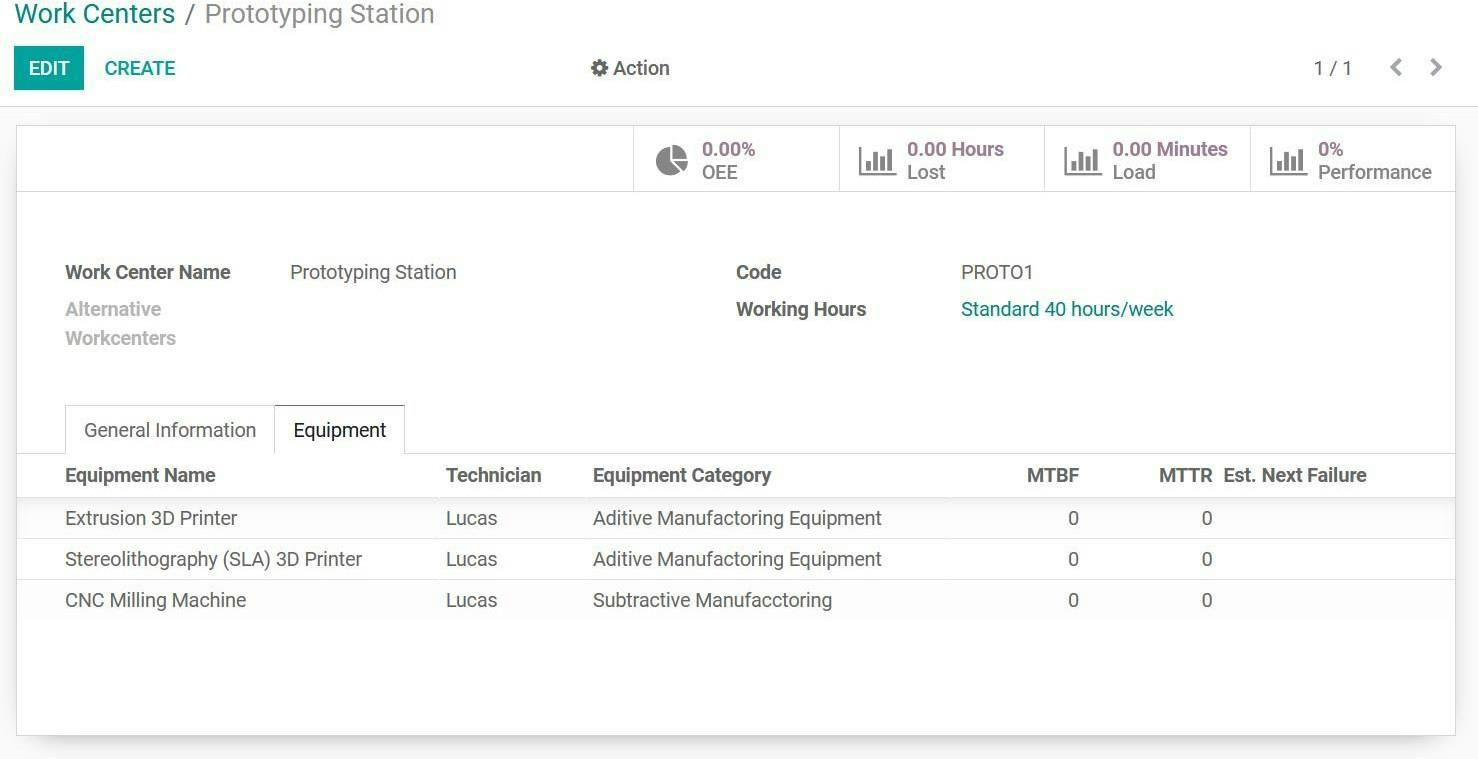
\includegraphics[width=433.7pt,height=222pt]{latexImage_bbdca77a67d2ff709f30917c132c2cc5.png}}
\put(73.15,-518.5){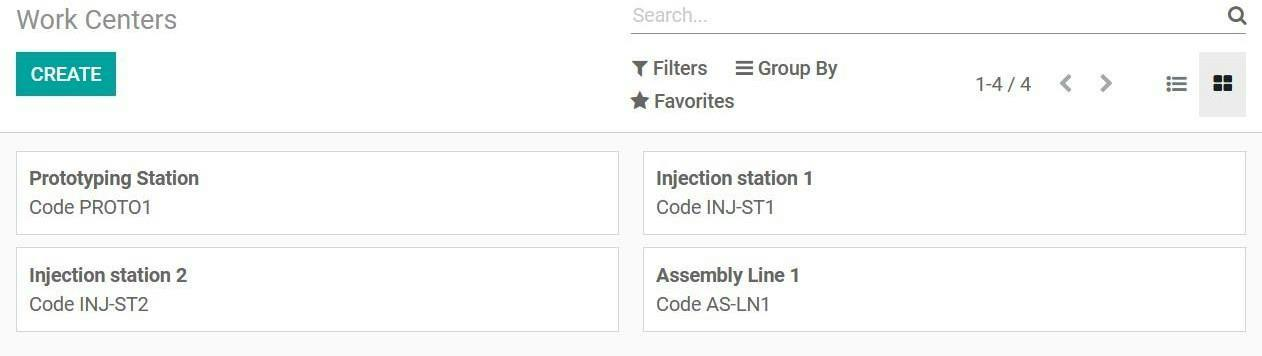
\includegraphics[width=428.23pt,height=120.1pt]{latexImage_ae8b8245b08ea487cf1339e86b557755.png}}
\put(69.384,-72.44){\fontsize{12}{1}\usefont{T1}{ptm}{m}{n}\selectfont\color{color_29791},並且因為它們在}
\put(164.532,-72.44){\fontsize{12}{1}\usefont{T1}{ptm}{m}{n}\selectfont\color{color_29791}很大}
\put(188.4,-72.44){\fontsize{12}{1}\usefont{T1}{ptm}{m}{n}\selectfont\color{color_29791}程度上是獨立的,}
\put(283.548,-72.44){\fontsize{12}{1}\usefont{T1}{ptm}{m}{n}\selectfont\color{color_29791}但是}
\put(307.416,-72.44){\fontsize{12}{1}\usefont{T1}{ptm}{m}{n}\selectfont\color{color_29791},為了這種類比,}
\put(402.564,-72.44){\fontsize{12}{1}\usefont{T1}{ptm}{m}{n}\selectfont\color{color_29791}這被}
\put(426.432,-72.44){\fontsize{12}{1}\usefont{T1}{ptm}{m}{n}\selectfont\color{color_29791}認為具有足夠}
\put(69.384,-90.46002){\fontsize{12}{1}\usefont{T1}{ptm}{m}{n}\selectfont\color{color_29791}的代表性。}
\put(128.9,-90.46002){\fontsize{12}{1}\usefont{T1}{ptm}{m}{n}\selectfont\color{color_29791} }
\put(63.024,-99.34003){\fontsize{2.52}{1}\usefont{T1}{ptm}{m}{n}\selectfont\color{color_29791} }
\put(229.73,-340.09){\fontsize{12}{1}\usefont{T1}{ptm}{b}{n}\selectfont\color{color_29791}圖}
\put(241.73,-340.09){\fontsize{12}{1}\usefont{T1}{ptm}{b}{n}\selectfont\color{color_29791} }
\put(244.73,-340.09){\fontsize{12}{1}\usefont{T1}{ptm}{b}{n}\selectfont\color{color_29791}34}
\put(256.73,-340.09){\fontsize{12}{1}\usefont{T1}{ptm}{b}{n}\selectfont\color{color_29791} }
\put(259.61,-340.09){\fontsize{12}{1}\usefont{T1}{ptm}{b}{n}\selectfont\color{color_29791}原型站專案表示}
\put(343.63,-340.09){\fontsize{12}{1}\usefont{T1}{ptm}{b}{n}\selectfont\color{color_29791} }
\put(346.63,-340.09){\fontsize{12}{1}\usefont{T1}{ptm}{b}{n}\selectfont\color{color_29791}2}
\put(352.27,-340.09){\fontsize{12}{1}\usefont{T1}{ptm}{b}{n}\selectfont\color{color_29791} }
\put(63.024,-357.25){\fontsize{12}{1}\usefont{T1}{ptm}{b}{n}\selectfont\color{color_29791} }
\put(82.944,-372.01){\fontsize{12}{1}\usefont{T1}{ptm}{m}{n}\selectfont\color{color_29791}還為類}
\put(118.824,-372.01){\fontsize{12}{1}\usefont{T1}{ptm}{m}{n}\selectfont\color{color_29791}比創建}
\put(154.704,-372.01){\fontsize{12}{1}\usefont{T1}{ptm}{m}{n}\selectfont\color{color_29791}了以}
\put(178.584,-372.01){\fontsize{12}{1}\usefont{T1}{ptm}{m}{n}\selectfont\color{color_29791}下工}
\put(202.464,-372.01){\fontsize{12}{1}\usefont{T1}{ptm}{m}{n}\selectfont\color{color_29791}作中心}
\put(238.344,-372.01){\fontsize{12}{1}\usefont{T1}{ptm}{m}{n}\selectfont\color{color_29791},並配}
\put(274.224,-372.01){\fontsize{12}{1}\usefont{T1}{ptm}{m}{n}\selectfont\color{color_29791}備了}
\put(298.104,-372.01){\fontsize{12}{1}\usefont{T1}{ptm}{m}{n}\selectfont\color{color_29791}必要}
\put(321.984,-372.01){\fontsize{12}{1}\usefont{T1}{ptm}{m}{n}\selectfont\color{color_29791}的設備}
\put(357.864,-372.01){\fontsize{12}{1}\usefont{T1}{ptm}{m}{n}\selectfont\color{color_29791}:}
\put(369.79,-372.01){\fontsize{12}{1}\usefont{T1}{ptm}{m}{n}\selectfont\color{color_29791} }
\put(63.024,-394.57){\fontsize{9.96}{1}\usefont{T1}{ptm}{m}{n}\selectfont\color{color_29791} }
\put(226.37,-533.91){\fontsize{12}{1}\usefont{T1}{ptm}{b}{n}\selectfont\color{color_29791}圖}
\put(238.25,-533.91){\fontsize{12}{1}\usefont{T1}{ptm}{b}{n}\selectfont\color{color_29791} }
\put(241.13,-533.91){\fontsize{12}{1}\usefont{T1}{ptm}{b}{n}\selectfont\color{color_29791}35}
\put(253.13,-533.91){\fontsize{12}{1}\usefont{T1}{ptm}{b}{n}\selectfont\color{color_29791} }
\put(255.77,-533.91){\fontsize{12}{1}\usefont{T1}{ptm}{b}{n}\selectfont\color{color_29791}Wor}
\put(279.05,-533.91){\fontsize{12}{1}\usefont{T1}{ptm}{b}{n}\selectfont\color{color_29791}k}
\put(285.758,-533.91){\fontsize{12}{1}\usefont{T1}{ptm}{b}{n}\selectfont\color{color_29791}c}
\put(291.146,-533.91){\fontsize{12}{1}\usefont{T1}{ptm}{b}{n}\selectfont\color{color_29791}e}
\put(296.426,-533.91){\fontsize{12}{1}\usefont{T1}{ptm}{b}{n}\selectfont\color{color_29791}n}
\put(303.134,-533.91){\fontsize{12}{1}\usefont{T1}{ptm}{b}{n}\selectfont\color{color_29791}te}
\put(312.374,-533.91){\fontsize{12}{1}\usefont{T1}{ptm}{b}{n}\selectfont\color{color_29791}r}
\put(317.83,-533.91){\fontsize{12}{1}\usefont{T1}{ptm}{b}{n}\selectfont\color{color_29791} }
\put(320.35,-533.91){\fontsize{12}{1}\usefont{T1}{ptm}{b}{n}\selectfont\color{color_29791}項}
\put(332.11,-533.91){\fontsize{12}{1}\usefont{T1}{ptm}{b}{n}\selectfont\color{color_29791}概}
\put(343.99,-533.91){\fontsize{12}{1}\usefont{T1}{ptm}{b}{n}\selectfont\color{color_29791}述}
\put(355.75,-533.91){\fontsize{12}{1}\usefont{T1}{ptm}{b}{n}\selectfont\color{color_29791} }
\put(87.38,-578.7){\fontsize{14.04}{1}\usefont{T1}{ptm}{b}{n}\selectfont\color{color_29791}5}
\put(94.44212,-578.7){\fontsize{14.04}{1}\usefont{T1}{ptm}{b}{n}\selectfont\color{color_29791}.4.}
\put(108.38,-578.7){\fontsize{14.04}{1}\usefont{T1}{ptm}{b}{n}\selectfont\color{color_29791} }
\put(111.74,-578.7){\fontsize{14.04}{1}\usefont{T1}{ptm}{b}{n}\selectfont\color{color_29791}開發}
\put(139.22,-578.7){\fontsize{14.04}{1}\usefont{T1}{ptm}{b}{n}\selectfont\color{color_29791} }
\put(82.944,-612.66){\fontsize{12}{1}\usefont{T1}{ptm}{m}{n}\selectfont\color{color_29791}現}
\put(94.94,-612.66){\fontsize{12}{1}\usefont{T1}{ptm}{m}{n}\selectfont\color{color_29791}在}
\put(106.94,-612.66){\fontsize{12}{1}\usefont{T1}{ptm}{m}{n}\selectfont\color{color_29791},公司的基本結構已在軟體中重新創建,可以開始模擬過程。首先,最引人}
\put(69.384,-630.54){\fontsize{12}{1}\usefont{T1}{ptm}{m}{n}\selectfont\color{color_29791}注目的是使用}
\put(141.38,-630.54){\fontsize{12}{1}\usefont{T1}{ptm}{m}{n}\selectfont\color{color_29791} }
\put(241.61,-630.54){\fontsize{12}{1}\usefont{T1}{ptm}{m}{n}\selectfont\color{color_29791}Odoo}
\put(268.25,-630.54){\fontsize{12}{1}\usefont{T1}{ptm}{m}{n}\selectfont\color{color_29791} }
\put(368.47,-630.54){\fontsize{12}{1}\usefont{T1}{ptm}{m}{n}\selectfont\color{color_29791}的全新產品的開發方面(}
\put(500.5,-630.54){\fontsize{12}{1}\usefont{T1}{ptm}{m}{n}\selectfont\color{color_29791}圖}
\put(511.66,-630.54){\fontsize{12}{1}\usefont{T1}{ptm}{m}{n}\selectfont\color{color_29791} }
\put(69.384,-648.42){\fontsize{12}{1}\usefont{T1}{ptm}{m}{n}\selectfont\color{color_29791}9}
\put(75.384,-648.42){\fontsize{12}{1}\usefont{T1}{ptm}{m}{n}\selectfont\color{color_29791})}
\put(87.38,-648.42){\fontsize{12}{1}\usefont{T1}{ptm}{m}{n}\selectfont\color{color_29791},}
\put(99.38,-648.42){\fontsize{12}{1}\usefont{T1}{ptm}{m}{n}\selectfont\color{color_29791}因為這是公司創建的第一款產品,因此評估了}
\put(339.43,-648.42){\fontsize{12}{1}\usefont{T1}{ptm}{m}{n}\selectfont\color{color_29791} }
\put(368.47,-648.42){\fontsize{12}{1}\usefont{T1}{ptm}{m}{n}\selectfont\color{color_29791} }
\put(485.98,-648.42){\fontsize{12}{1}\usefont{T1}{ptm}{m}{n}\selectfont\color{color_29791}O}
\put(494.38,-648.42){\fontsize{12}{1}\usefont{T1}{ptm}{m}{n}\selectfont\color{color_29791}d}
\put(500.14,-648.42){\fontsize{12}{1}\usefont{T1}{ptm}{m}{n}\selectfont\color{color_29791}o}
\put(505.9,-648.42){\fontsize{12}{1}\usefont{T1}{ptm}{m}{n}\selectfont\color{color_29791}o}
\put(69.384,-666.3){\fontsize{12}{1}\usefont{T1}{ptm}{m}{n}\selectfont\color{color_29791}用於組織原型製作程式的可能性。這包括從構思到設計和原型生產的路}
\put(441.46,-666.3){\fontsize{12}{1}\usefont{T1}{ptm}{m}{n}\selectfont\color{color_29791}徑}
\put(453.46,-666.3){\fontsize{12}{1}\usefont{T1}{ptm}{m}{n}\selectfont\color{color_29791}。然後,}
\put(69.384,-684.176){\fontsize{12}{1}\usefont{T1}{ptm}{m}{n}\selectfont\color{color_29791}一旦產品作為原型達到可接受的結果,就會進行有關生產過程開發的工}
\put(441.46,-684.176){\fontsize{12}{1}\usefont{T1}{ptm}{m}{n}\selectfont\color{color_29791}作}
\put(453.46,-684.176){\fontsize{12}{1}\usefont{T1}{ptm}{m}{n}\selectfont\color{color_29791}。一旦正}
\put(69.384,-702.176){\fontsize{12}{1}\usefont{T1}{ptm}{m}{n}\selectfont\color{color_29791}式生產運行完}
\put(141.38,-702.176){\fontsize{12}{1}\usefont{T1}{ptm}{m}{n}\selectfont\color{color_29791}成}
\put(153.38,-702.176){\fontsize{12}{1}\usefont{T1}{ptm}{m}{n}\selectfont\color{color_29791},產品開發就被認為是成功的。}
\put(321.43,-702.176){\fontsize{12}{1}\usefont{T1}{ptm}{m}{n}\selectfont\color{color_29791} }
\end{picture}
\newpage
\begin{tikzpicture}[overlay]\path(0pt,0pt);\end{tikzpicture}
\begin{picture}(-5,0)(2.5,0)
\put(500.26,-727.616){\fontsize{12}{1}\usefont{T1}{ptm}{m}{n}\selectfont\color{color_29791}42}
\put(511.78,-727.616){\fontsize{12}{1}\usefont{T1}{ptm}{m}{n}\selectfont\color{color_29791} }
\put(63.024,-726.896){\fontsize{9.96}{1}\usefont{T1}{ptm}{m}{n}\selectfont\color{color_29791} }
\put(193.55,-312.63){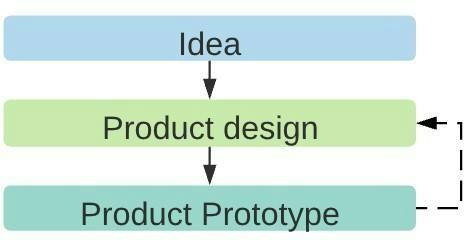
\includegraphics[width=198.4pt,height=102.58pt]{latexImage_b553a4b3a8e0d0192d273754ab898535.png}}
\put(105.38,-90.46002){\fontsize{12.81913}{1}\usefont{T1}{ptm}{b}{n}\selectfont\color{color_29791}5.}
\put(114.9648,-90.46002){\fontsize{12.81913}{1}\usefont{T1}{ptm}{b}{n}\selectfont\color{color_29791}4}
\put(121.4307,-90.46002){\fontsize{12.81913}{1}\usefont{T1}{ptm}{b}{n}\selectfont\color{color_29791}.}
\put(124.5495,-90.46002){\fontsize{12.81913}{1}\usefont{T1}{ptm}{b}{n}\selectfont\color{color_29791}1}
\put(131.0154,-90.46002){\fontsize{12.81913}{1}\usefont{T1}{ptm}{b}{n}\selectfont\color{color_29791}.}
\put(134.3,-90.46002){\fontsize{12.83539}{1}\usefont{T1}{ptm}{b}{n}\selectfont\color{color_29791} }
\put(137.66,-90.46002){\fontsize{12.96}{1}\usefont{T1}{ptm}{b}{n}\selectfont\color{color_29791}創意}
\put(163.58,-90.46002){\fontsize{12.96}{1}\usefont{T1}{ptm}{b}{n}\selectfont\color{color_29791} }
\put(166.82,-90.46002){\fontsize{12.96}{1}\usefont{T1}{ptm}{b}{n}\selectfont\color{color_29791}-}
\put(171.02,-90.46002){\fontsize{12.96}{1}\usefont{T1}{ptm}{b}{n}\selectfont\color{color_29791} }
\put(174.14,-90.46002){\fontsize{12.96}{1}\usefont{T1}{ptm}{b}{n}\selectfont\color{color_29791}設計}
\put(200.09,-90.46002){\fontsize{12.96}{1}\usefont{T1}{ptm}{b}{n}\selectfont\color{color_29791} }
\put(203.33,-90.46002){\fontsize{12.96}{1}\usefont{T1}{ptm}{b}{n}\selectfont\color{color_29791}-}
\put(207.53,-90.46002){\fontsize{12.96}{1}\usefont{T1}{ptm}{b}{n}\selectfont\color{color_29791} }
\put(210.65,-90.46002){\fontsize{12.96}{1}\usefont{T1}{ptm}{b}{n}\selectfont\color{color_29791}產品原型}
\put(262.01,-90.46002){\fontsize{12.96}{1}\usefont{T1}{ptm}{b}{n}\selectfont\color{color_29791} }
\put(82.944,-117.22){\fontsize{12}{1}\usefont{T1}{ptm}{m}{n}\selectfont\color{color_29791}如(第}
\put(118.58,-117.22){\fontsize{12}{1}\usefont{T1}{ptm}{m}{n}\selectfont\color{color_29791}4}
\put(124.46,-117.22){\fontsize{12}{1}\usefont{T1}{ptm}{m}{n}\selectfont\color{color_29791}章}
\put(136.34,-117.22){\fontsize{12}{1}\usefont{T1}{ptm}{m}{n}\selectfont\color{color_29791})}
\put(148.22,-117.22){\fontsize{12}{1}\usefont{T1}{ptm}{m}{n}\selectfont\color{color_29791}所}
\put(160.1,-117.22){\fontsize{12}{1}\usefont{T1}{ptm}{m}{n}\selectfont\color{color_29791}述,}
\put(183.98,-117.22){\fontsize{12}{1}\usefont{T1}{ptm}{m}{n}\selectfont\color{color_29791}產品}
\put(207.86,-117.22){\fontsize{12}{1}\usefont{T1}{ptm}{m}{n}\selectfont\color{color_29791}的}
\put(219.74,-117.22){\fontsize{12}{1}\usefont{T1}{ptm}{m}{n}\selectfont\color{color_29791}想}
\put(231.62,-117.22){\fontsize{12}{1}\usefont{T1}{ptm}{m}{n}\selectfont\color{color_29791}法}
\put(243.5,-117.22){\fontsize{12}{1}\usefont{T1}{ptm}{m}{n}\selectfont\color{color_29791}已}
\put(255.38,-117.22){\fontsize{12}{1}\usefont{T1}{ptm}{m}{n}\selectfont\color{color_29791}經}
\put(267.26,-117.22){\fontsize{12}{1}\usefont{T1}{ptm}{m}{n}\selectfont\color{color_29791}確}
\put(279.14,-117.22){\fontsize{12}{1}\usefont{T1}{ptm}{m}{n}\selectfont\color{color_29791}定,}
\put(303.0201,-117.22){\fontsize{12}{1}\usefont{T1}{ptm}{m}{n}\selectfont\color{color_29791}初步}
\put(326.9001,-117.22){\fontsize{12}{1}\usefont{T1}{ptm}{m}{n}\selectfont\color{color_29791}的}
\put(338.7801,-117.22){\fontsize{12}{1}\usefont{T1}{ptm}{m}{n}\selectfont\color{color_29791}設}
\put(350.6601,-117.22){\fontsize{12}{1}\usefont{T1}{ptm}{m}{n}\selectfont\color{color_29791}計}
\put(362.5401,-117.22){\fontsize{12}{1}\usefont{T1}{ptm}{m}{n}\selectfont\color{color_29791}特}
\put(374.4201,-117.22){\fontsize{12}{1}\usefont{T1}{ptm}{m}{n}\selectfont\color{color_29791}徵}
\put(386.3001,-117.22){\fontsize{12}{1}\usefont{T1}{ptm}{m}{n}\selectfont\color{color_29791}和}
\put(398.1801,-117.22){\fontsize{12}{1}\usefont{T1}{ptm}{m}{n}\selectfont\color{color_29791}基礎}
\put(422.0601,-117.22){\fontsize{12}{1}\usefont{T1}{ptm}{m}{n}\selectfont\color{color_29791}產品}
\put(445.9401,-117.22){\fontsize{12}{1}\usefont{T1}{ptm}{m}{n}\selectfont\color{color_29791}研}
\put(457.8201,-117.22){\fontsize{12}{1}\usefont{T1}{ptm}{m}{n}\selectfont\color{color_29791}究}
\put(469.7001,-117.22){\fontsize{12}{1}\usefont{T1}{ptm}{m}{n}\selectfont\color{color_29791}已}
\put(481.5801,-117.22){\fontsize{12}{1}\usefont{T1}{ptm}{m}{n}\selectfont\color{color_29791}經}
\put(493.4601,-117.22){\fontsize{12}{1}\usefont{T1}{ptm}{m}{n}\selectfont\color{color_29791}進}
\put(69.384,-135.1){\fontsize{12}{1}\usefont{T1}{ptm}{m}{n}\selectfont\color{color_29791}行。這代表了}
\put(140.66,-135.1){\fontsize{12}{1}\usefont{T1}{ptm}{m}{n}\selectfont\color{color_29791}Od}
\put(155.18,-135.1){\fontsize{12}{1}\usefont{T1}{ptm}{m}{n}\selectfont\color{color_29791}o}
\put(161.06,-135.1){\fontsize{12}{1}\usefont{T1}{ptm}{m}{n}\selectfont\color{color_29791}o}
\put(166.94,-135.1){\fontsize{12}{1}\usefont{T1}{ptm}{m}{n}\selectfont\color{color_29791}軟}
\put(178.82,-135.1){\fontsize{12}{1}\usefont{T1}{ptm}{m}{n}\selectfont\color{color_29791}體在}
\put(202.7,-135.1){\fontsize{12}{1}\usefont{T1}{ptm}{m}{n}\selectfont\color{color_29791}現}
\put(214.58,-135.1){\fontsize{12}{1}\usefont{T1}{ptm}{m}{n}\selectfont\color{color_29791}實}
\put(226.46,-135.1){\fontsize{12}{1}\usefont{T1}{ptm}{m}{n}\selectfont\color{color_29791}世}
\put(238.34,-135.1){\fontsize{12}{1}\usefont{T1}{ptm}{m}{n}\selectfont\color{color_29791}界}
\put(250.22,-135.1){\fontsize{12}{1}\usefont{T1}{ptm}{m}{n}\selectfont\color{color_29791}中}
\put(262.1,-135.1){\fontsize{12}{1}\usefont{T1}{ptm}{m}{n}\selectfont\color{color_29791}的}
\put(273.98,-135.1){\fontsize{12}{1}\usefont{T1}{ptm}{m}{n}\selectfont\color{color_29791}實際}
\put(297.86,-135.1){\fontsize{12}{1}\usefont{T1}{ptm}{m}{n}\selectfont\color{color_29791}實施}
\put(321.7401,-135.1){\fontsize{12}{1}\usefont{T1}{ptm}{m}{n}\selectfont\color{color_29791},}
\put(333.6201,-135.1){\fontsize{12}{1}\usefont{T1}{ptm}{m}{n}\selectfont\color{color_29791}因}
\put(345.5001,-135.1){\fontsize{12}{1}\usefont{T1}{ptm}{m}{n}\selectfont\color{color_29791}為}
\put(357.3801,-135.1){\fontsize{12}{1}\usefont{T1}{ptm}{m}{n}\selectfont\color{color_29791}儘}
\put(369.2601,-135.1){\fontsize{12}{1}\usefont{T1}{ptm}{m}{n}\selectfont\color{color_29791}管}
\put(381.19,-135.1){\fontsize{12}{1}\usefont{T1}{ptm}{m}{n}\selectfont\color{color_29791}Od}
\put(395.71,-135.1){\fontsize{12}{1}\usefont{T1}{ptm}{m}{n}\selectfont\color{color_29791}o}
\put(401.59,-135.1){\fontsize{12}{1}\usefont{T1}{ptm}{m}{n}\selectfont\color{color_29791}o}
\put(407.47,-135.1){\fontsize{12}{1}\usefont{T1}{ptm}{m}{n}\selectfont\color{color_29791}具}
\put(419.35,-135.1){\fontsize{12}{1}\usefont{T1}{ptm}{m}{n}\selectfont\color{color_29791}有良}
\put(443.23,-135.1){\fontsize{12}{1}\usefont{T1}{ptm}{m}{n}\selectfont\color{color_29791}好}
\put(455.11,-135.1){\fontsize{12}{1}\usefont{T1}{ptm}{m}{n}\selectfont\color{color_29791}的}
\put(466.99,-135.1){\fontsize{12}{1}\usefont{T1}{ptm}{m}{n}\selectfont\color{color_29791}專}
\put(478.87,-135.1){\fontsize{12}{1}\usefont{T1}{ptm}{m}{n}\selectfont\color{color_29791}案}
\put(490.75,-135.1){\fontsize{12}{1}\usefont{T1}{ptm}{m}{n}\selectfont\color{color_29791}管}
\put(69.384,-152.98){\fontsize{12}{1}\usefont{T1}{ptm}{m}{n}\selectfont\color{color_29791}理和通信應用程式}
\put(164.532,-152.98){\fontsize{12}{1}\usefont{T1}{ptm}{m}{n}\selectfont\color{color_29791},但}
\put(188.4,-152.98){\fontsize{12}{1}\usefont{T1}{ptm}{m}{n}\selectfont\color{color_29791}這些應用程式是庫}
\put(283.548,-152.98){\fontsize{12}{1}\usefont{T1}{ptm}{m}{n}\selectfont\color{color_29791}存和}
\put(307.416,-152.98){\fontsize{12}{1}\usefont{T1}{ptm}{m}{n}\selectfont\color{color_29791}製造應用程式的外}
\put(402.564,-152.98){\fontsize{12}{1}\usefont{T1}{ptm}{m}{n}\selectfont\color{color_29791}部,}
\put(426.432,-152.98){\fontsize{12}{1}\usefont{T1}{ptm}{m}{n}\selectfont\color{color_29791}更重要的是,}
\put(69.384,-170.98){\fontsize{12}{1}\usefont{T1}{ptm}{m}{n}\selectfont\color{color_29791}與工程設計}
\put(128.78,-170.98){\fontsize{12}{1}\usefont{T1}{ptm}{m}{n}\selectfont\color{color_29791}C}
\put(136.7,-170.98){\fontsize{12}{1}\usefont{T1}{ptm}{m}{n}\selectfont\color{color_29791}AD}
\put(153.86,-170.98){\fontsize{12}{1}\usefont{T1}{ptm}{m}{n}\selectfont\color{color_29791}軟}
\put(165.74,-170.98){\fontsize{12}{1}\usefont{T1}{ptm}{m}{n}\selectfont\color{color_29791}體}
\put(177.62,-170.98){\fontsize{12}{1}\usefont{T1}{ptm}{m}{n}\selectfont\color{color_29791}沒有}
\put(201.5,-170.98){\fontsize{12}{1}\usefont{T1}{ptm}{m}{n}\selectfont\color{color_29791}集}
\put(213.38,-170.98){\fontsize{12}{1}\usefont{T1}{ptm}{m}{n}\selectfont\color{color_29791}成}
\put(225.26,-170.98){\fontsize{12}{1}\usefont{T1}{ptm}{m}{n}\selectfont\color{color_29791}。}
\put(237.14,-170.98){\fontsize{12}{1}\usefont{T1}{ptm}{m}{n}\selectfont\color{color_29791}在}
\put(249.02,-170.98){\fontsize{12}{1}\usefont{T1}{ptm}{m}{n}\selectfont\color{color_29791}這}
\put(260.9,-170.98){\fontsize{12}{1}\usefont{T1}{ptm}{m}{n}\selectfont\color{color_29791}個}
\put(272.78,-170.98){\fontsize{12}{1}\usefont{T1}{ptm}{m}{n}\selectfont\color{color_29791}類比}
\put(296.66,-170.98){\fontsize{12}{1}\usefont{T1}{ptm}{m}{n}\selectfont\color{color_29791}中,}
\put(320.54,-170.98){\fontsize{12}{1}\usefont{T1}{ptm}{m}{n}\selectfont\color{color_29791}這}
\put(332.42,-170.98){\fontsize{12}{1}\usefont{T1}{ptm}{m}{n}\selectfont\color{color_29791}個}
\put(344.3,-170.98){\fontsize{12}{1}\usefont{T1}{ptm}{m}{n}\selectfont\color{color_29791}想}
\put(356.1801,-170.98){\fontsize{12}{1}\usefont{T1}{ptm}{m}{n}\selectfont\color{color_29791}法}
\put(368.0601,-170.98){\fontsize{12}{1}\usefont{T1}{ptm}{m}{n}\selectfont\color{color_29791}已}
\put(379.9401,-170.98){\fontsize{12}{1}\usefont{T1}{ptm}{m}{n}\selectfont\color{color_29791}經}
\put(391.8201,-170.98){\fontsize{12}{1}\usefont{T1}{ptm}{m}{n}\selectfont\color{color_29791}付諸}
\put(415.7001,-170.98){\fontsize{12}{1}\usefont{T1}{ptm}{m}{n}\selectfont\color{color_29791}實踐}
\put(439.5801,-170.98){\fontsize{12}{1}\usefont{T1}{ptm}{m}{n}\selectfont\color{color_29791},}
\put(451.4601,-170.98){\fontsize{12}{1}\usefont{T1}{ptm}{m}{n}\selectfont\color{color_29791}並}
\put(463.3401,-170.98){\fontsize{12}{1}\usefont{T1}{ptm}{m}{n}\selectfont\color{color_29791}使}
\put(475.2201,-170.98){\fontsize{12}{1}\usefont{T1}{ptm}{m}{n}\selectfont\color{color_29791}用}
\put(487.18,-170.98){\fontsize{12}{1}\usefont{T1}{ptm}{m}{n}\selectfont\color{color_29791} }
\put(69.384,-188.86){\fontsize{12}{1}\usefont{T1}{ptm}{m}{n}\selectfont\color{color_29791}S}
\put(76.092,-188.86){\fontsize{12}{1}\usefont{T1}{ptm}{m}{n}\selectfont\color{color_29791}oli}
\put(88.8,-188.86){\fontsize{12}{1}\usefont{T1}{ptm}{m}{n}\selectfont\color{color_29791}dwor}
\put(113.4,-188.86){\fontsize{12}{1}\usefont{T1}{ptm}{m}{n}\selectfont\color{color_29791}ks }
\put(127.1,-188.86){\fontsize{12}{1}\usefont{T1}{ptm}{m}{n}\selectfont\color{color_29791}軟體轉化為}
\put(185.93,-188.86){\fontsize{12}{1}\usefont{T1}{ptm}{m}{n}\selectfont\color{color_29791} }
\put(191.57,-188.86){\fontsize{12}{1}\usefont{T1}{ptm}{m}{n}\selectfont\color{color_29791}C}
\put(199.598,-188.86){\fontsize{12}{1}\usefont{T1}{ptm}{m}{n}\selectfont\color{color_29791}AD}
\put(216.878,-188.86){\fontsize{12}{1}\usefont{T1}{ptm}{m}{n}\selectfont\color{color_29791} }
\put(219.89,-188.86){\fontsize{12}{1}\usefont{T1}{ptm}{m}{n}\selectfont\color{color_29791}設}
\put(231.77,-188.86){\fontsize{12}{1}\usefont{T1}{ptm}{m}{n}\selectfont\color{color_29791}計}
\put(243.65,-188.86){\fontsize{12}{1}\usefont{T1}{ptm}{m}{n}\selectfont\color{color_29791},}
\put(255.53,-188.86){\fontsize{12}{1}\usefont{T1}{ptm}{m}{n}\selectfont\color{color_29791}生}
\put(267.41,-188.86){\fontsize{12}{1}\usefont{T1}{ptm}{m}{n}\selectfont\color{color_29791}成}
\put(279.29,-188.86){\fontsize{12}{1}\usefont{T1}{ptm}{m}{n}\selectfont\color{color_29791}本}
\put(291.17,-188.86){\fontsize{12}{1}\usefont{T1}{ptm}{m}{n}\selectfont\color{color_29791}地存}
\put(315.05,-188.86){\fontsize{12}{1}\usefont{T1}{ptm}{m}{n}\selectfont\color{color_29791}儲}
\put(326.93,-188.86){\fontsize{12}{1}\usefont{T1}{ptm}{m}{n}\selectfont\color{color_29791}在}
\put(338.81,-188.86){\fontsize{12}{1}\usefont{T1}{ptm}{m}{n}\selectfont\color{color_29791}工}
\put(350.69,-188.86){\fontsize{12}{1}\usefont{T1}{ptm}{m}{n}\selectfont\color{color_29791}程}
\put(362.57,-188.86){\fontsize{12}{1}\usefont{T1}{ptm}{m}{n}\selectfont\color{color_29791}師}
\put(374.45,-188.86){\fontsize{12}{1}\usefont{T1}{ptm}{m}{n}\selectfont\color{color_29791}計}
\put(386.33,-188.86){\fontsize{12}{1}\usefont{T1}{ptm}{m}{n}\selectfont\color{color_29791}算機}
\put(410.2101,-188.86){\fontsize{12}{1}\usefont{T1}{ptm}{m}{n}\selectfont\color{color_29791}中的}
\put(434.11,-188.86){\fontsize{12}{1}\usefont{T1}{ptm}{m}{n}\selectfont\color{color_29791} }
\put(440.02,-188.86){\fontsize{12}{1}\usefont{T1}{ptm}{m}{n}\selectfont\color{color_29791}C}
\put(448.048,-188.86){\fontsize{12}{1}\usefont{T1}{ptm}{m}{n}\selectfont\color{color_29791}AD}
\put(465.328,-188.86){\fontsize{12}{1}\usefont{T1}{ptm}{m}{n}\selectfont\color{color_29791} }
\put(468.34,-188.86){\fontsize{12}{1}\usefont{T1}{ptm}{m}{n}\selectfont\color{color_29791}檔。}
\put(492.46,-188.86){\fontsize{12}{1}\usefont{T1}{ptm}{m}{n}\selectfont\color{color_29791} }
\put(63.024,-206.14){\fontsize{9.96}{1}\usefont{T1}{ptm}{m}{n}\selectfont\color{color_29791} }
\put(231.53,-336.61){\fontsize{12}{1}\usefont{T1}{ptm}{b}{n}\selectfont\color{color_29791}圖}
\put(243.53,-336.61){\fontsize{12}{1}\usefont{T1}{ptm}{b}{n}\selectfont\color{color_29791}36}
\put(255.53,-336.61){\fontsize{12}{1}\usefont{T1}{ptm}{b}{n}\selectfont\color{color_29791}產品開發的剖面圖}
\put(350.71,-336.61){\fontsize{12}{1}\usefont{T1}{ptm}{b}{n}\selectfont\color{color_29791} }
\put(82.944,-368.41){\fontsize{12}{1}\usefont{T1}{ptm}{m}{n}\selectfont\color{color_29791}正是在這一點上,}
\put(178.1,-368.41){\fontsize{12}{1}\usefont{T1}{ptm}{m}{n}\selectfont\color{color_29791}O}
\put(186.62,-368.41){\fontsize{12}{1}\usefont{T1}{ptm}{m}{n}\selectfont\color{color_29791}d}
\put(192.5,-368.41){\fontsize{12}{1}\usefont{T1}{ptm}{m}{n}\selectfont\color{color_29791}o}
\put(198.38,-368.41){\fontsize{12}{1}\usefont{T1}{ptm}{m}{n}\selectfont\color{color_29791}o}
\put(204.41,-368.41){\fontsize{12}{1}\usefont{T1}{ptm}{m}{n}\selectfont\color{color_29791}軟體的正式使用可}
\put(299.558,-368.41){\fontsize{12}{1}\usefont{T1}{ptm}{m}{n}\selectfont\color{color_29791}以正}
\put(323.426,-368.41){\fontsize{12}{1}\usefont{T1}{ptm}{m}{n}\selectfont\color{color_29791}式發生。第一步是}
\put(418.574,-368.41){\fontsize{12}{1}\usefont{T1}{ptm}{m}{n}\selectfont\color{color_29791}瞭解}
\put(442.442,-368.41){\fontsize{12}{1}\usefont{T1}{ptm}{m}{n}\selectfont\color{color_29791}就產品專案}
\put(69.384,-386.41){\fontsize{12}{1}\usefont{T1}{ptm}{m}{n}\selectfont\color{color_29791}而言,生產主題是}
\put(164.532,-386.41){\fontsize{12}{1}\usefont{T1}{ptm}{m}{n}\selectfont\color{color_29791}什麼}
\put(188.4,-386.41){\fontsize{12}{1}\usefont{T1}{ptm}{m}{n}\selectfont\color{color_29791}。如何做到這一點}
\put(283.548,-386.41){\fontsize{12}{1}\usefont{T1}{ptm}{m}{n}\selectfont\color{color_29791}有兩}
\put(307.416,-386.41){\fontsize{12}{1}\usefont{T1}{ptm}{m}{n}\selectfont\color{color_29791}種方法:}
\put(355.15,-386.41){\fontsize{12}{1}\usefont{T1}{ptm}{m}{n}\selectfont\color{color_29791} }
\put(105.14,-419.31){\fontsize{12}{1}\usefont{T1}{ptm}{m}{n}\selectfont\color{color_29791}}
\put(115.82,-419.31){\fontsize{12}{1}\usefont{T1}{uarial}{m}{n}\selectfont\color{color_29791} }
\put(123.14,-419.31){\fontsize{12}{1}\usefont{T1}{ptm}{m}{n}\selectfont\color{color_29791}第一種是將原型視}
\put(219.248,-419.31){\fontsize{12}{1}\usefont{T1}{ptm}{m}{n}\selectfont\color{color_29791}為最}
\put(243.356,-419.31){\fontsize{12}{1}\usefont{T1}{ptm}{m}{n}\selectfont\color{color_29791}終產品的早期修訂}
\put(339.464,-419.31){\fontsize{12}{1}\usefont{T1}{ptm}{m}{n}\selectfont\color{color_29791}版,}
\put(363.572,-419.31){\fontsize{12}{1}\usefont{T1}{ptm}{m}{n}\selectfont\color{color_29791}也就是說,在}
\put(435.67,-419.31){\fontsize{12}{1}\usefont{T1}{ptm}{m}{n}\selectfont\color{color_29791}Od}
\put(450.19,-419.31){\fontsize{12}{1}\usefont{T1}{ptm}{m}{n}\selectfont\color{color_29791}o}
\put(456.07,-419.31){\fontsize{12}{1}\usefont{T1}{ptm}{m}{n}\selectfont\color{color_29791}o}
\put(462.1,-419.31){\fontsize{12}{1}\usefont{T1}{ptm}{m}{n}\selectfont\color{color_29791}中創}
\put(486.208,-419.31){\fontsize{12}{1}\usefont{T1}{ptm}{m}{n}\selectfont\color{color_29791}建的}
\put(123.14,-437.19){\fontsize{12}{1}\usefont{T1}{ptm}{m}{n}\selectfont\color{color_29791}原型專案將與最終}
\put(219.98,-437.19){\fontsize{12}{1}\usefont{T1}{ptm}{m}{n}\selectfont\color{color_29791}產品}
\put(244.1,-437.19){\fontsize{12}{1}\usefont{T1}{ptm}{m}{n}\selectfont\color{color_29791}專案相同,並在開}
\put(340.94,-437.19){\fontsize{12}{1}\usefont{T1}{ptm}{m}{n}\selectfont\color{color_29791}發過}
\put(365.06,-437.19){\fontsize{12}{1}\usefont{T1}{ptm}{m}{n}\selectfont\color{color_29791}程中進行了修改。}
\put(461.9,-437.19){\fontsize{12}{1}\usefont{T1}{ptm}{m}{n}\selectfont\color{color_29791}如果}
\put(486.02,-437.19){\fontsize{12}{1}\usefont{T1}{ptm}{m}{n}\selectfont\color{color_29791}原型}
\put(123.14,-455.07){\fontsize{12}{1}\usefont{T1}{ptm}{m}{n}\selectfont\color{color_29791}是通過與最終生產}
\put(219.98,-455.07){\fontsize{12}{1}\usefont{T1}{ptm}{m}{n}\selectfont\color{color_29791}中使}
\put(244.1,-455.07){\fontsize{12}{1}\usefont{T1}{ptm}{m}{n}\selectfont\color{color_29791}用的方法相同的方}
\put(340.94,-455.07){\fontsize{12}{1}\usefont{T1}{ptm}{m}{n}\selectfont\color{color_29791}法實}
\put(365.06,-455.07){\fontsize{12}{1}\usefont{T1}{ptm}{m}{n}\selectfont\color{color_29791}現的,則建議這樣}
\put(461.9,-455.07){\fontsize{12}{1}\usefont{T1}{ptm}{m}{n}\selectfont\color{color_29791}做。}
\put(486.02,-455.07){\fontsize{12}{1}\usefont{T1}{ptm}{m}{n}\selectfont\color{color_29791}這種}
\put(123.14,-472.95){\fontsize{12}{1}\usefont{T1}{ptm}{m}{n}\selectfont\color{color_29791}方法的一個例子是}
\put(219.98,-472.95){\fontsize{12}{1}\usefont{T1}{ptm}{m}{n}\selectfont\color{color_29791},如}
\put(244.1,-472.95){\fontsize{12}{1}\usefont{T1}{ptm}{m}{n}\selectfont\color{color_29791}果產品足夠簡單,}
\put(340.94,-472.95){\fontsize{12}{1}\usefont{T1}{ptm}{m}{n}\selectfont\color{color_29791}可以}
\put(365.06,-472.95){\fontsize{12}{1}\usefont{T1}{ptm}{m}{n}\selectfont\color{color_29791}同時進行產品和生}
\put(461.9,-472.95){\fontsize{12}{1}\usefont{T1}{ptm}{m}{n}\selectfont\color{color_29791}產方}
\put(486.02,-472.95){\fontsize{12}{1}\usefont{T1}{ptm}{m}{n}\selectfont\color{color_29791}面的}
\put(123.14,-490.83){\fontsize{12}{1}\usefont{T1}{ptm}{m}{n}\selectfont\color{color_29791}開發。}
\put(158.54,-490.83){\fontsize{12}{1}\usefont{T1}{ptm}{m}{n}\selectfont\color{color_29791} }
\put(105.14,-523.47){\fontsize{12}{1}\usefont{T1}{ptm}{m}{n}\selectfont\color{color_29791}}
\put(115.82,-523.47){\fontsize{12}{1}\usefont{T1}{uarial}{m}{n}\selectfont\color{color_29791} }
\put(123.14,-523.47){\fontsize{12}{1}\usefont{T1}{ptm}{m}{n}\selectfont\color{color_29791}第二個是將原型視}
\put(218.288,-523.47){\fontsize{12}{1}\usefont{T1}{ptm}{m}{n}\selectfont\color{color_29791}為與}
\put(242.156,-523.47){\fontsize{12}{1}\usefont{T1}{ptm}{m}{n}\selectfont\color{color_29791}最終產品分開的專}
\put(337.304,-523.47){\fontsize{12}{1}\usefont{T1}{ptm}{m}{n}\selectfont\color{color_29791}案}
\put(349.39,-523.47){\fontsize{12}{1}\usefont{T1}{ptm}{m}{n}\selectfont\color{color_29791} }
\put(508.66,-523.47){\fontsize{12}{1}\usefont{T1}{ptm}{m}{n}\selectfont\color{color_29791}-}
\put(123.14,-541.47){\fontsize{12}{1}\usefont{T1}{ptm}{m}{n}\selectfont\color{color_29791}這是該類比中採用的}
\put(232.1,-541.47){\fontsize{12}{1}\usefont{T1}{ptm}{m}{n}\selectfont\color{color_29791}路}
\put(244.1,-541.47){\fontsize{12}{1}\usefont{T1}{ptm}{m}{n}\selectfont\color{color_29791}徑。做出這一決定的}
\put(353.06,-541.47){\fontsize{12}{1}\usefont{T1}{ptm}{m}{n}\selectfont\color{color_29791}主}
\put(365.06,-541.47){\fontsize{12}{1}\usefont{T1}{ptm}{m}{n}\selectfont\color{color_29791}要原因是,由於原型}
\put(474.02,-541.47){\fontsize{12}{1}\usefont{T1}{ptm}{m}{n}\selectfont\color{color_29791}使}
\put(486.02,-541.47){\fontsize{12}{1}\usefont{T1}{ptm}{m}{n}\selectfont\color{color_29791}用}
\put(498.22,-541.47){\fontsize{12}{1}\usefont{T1}{ptm}{m}{n}\selectfont\color{color_29791}3D}
\put(123.14,-559.35){\fontsize{12}{1}\usefont{T1}{ptm}{m}{n}\selectfont\color{color_29791}列印,因此我們的}
\put(218.288,-559.35){\fontsize{12}{1}\usefont{T1}{ptm}{m}{n}\selectfont\color{color_29791}原型}
\put(242.156,-559.35){\fontsize{12}{1}\usefont{T1}{ptm}{m}{n}\selectfont\color{color_29791}生產方式與最終生}
\put(337.304,-559.35){\fontsize{12}{1}\usefont{T1}{ptm}{m}{n}\selectfont\color{color_29791}產方}
\put(361.172,-559.35){\fontsize{12}{1}\usefont{T1}{ptm}{m}{n}\selectfont\color{color_29791}式不同。}
\put(408.91,-559.35){\fontsize{12}{1}\usefont{T1}{ptm}{m}{n}\selectfont\color{color_29791} }
\put(82.944,-592.26){\fontsize{12}{1}\usefont{T1}{ptm}{m}{n}\selectfont\color{color_29791}從根開}
\put(119.052,-592.26){\fontsize{12}{1}\usefont{T1}{ptm}{m}{n}\selectfont\color{color_29791}始,}
\put(143.16,-592.26){\fontsize{12}{1}\usefont{T1}{ptm}{m}{n}\selectfont\color{color_29791}創建了}
\put(179.268,-592.26){\fontsize{12}{1}\usefont{T1}{ptm}{m}{n}\selectfont\color{color_29791}一個}
\put(203.376,-592.26){\fontsize{12}{1}\usefont{T1}{ptm}{m}{n}\selectfont\color{color_29791}名為}
\put(227.45,-592.26){\fontsize{12}{1}\usefont{T1}{ptm}{m}{n}\selectfont\color{color_29791} }
\put(233.45,-592.26){\fontsize{12}{1}\usefont{T1}{ptm}{m}{n}\selectfont\color{color_29791}P}
\put(240.158,-592.26){\fontsize{12}{1}\usefont{T1}{ptm}{m}{n}\selectfont\color{color_29791}R}
\put(248.186,-592.26){\fontsize{12}{1}\usefont{T1}{ptm}{m}{n}\selectfont\color{color_29791}OT}
\put(264.146,-592.26){\fontsize{12}{1}\usefont{T1}{ptm}{m}{n}\selectfont\color{color_29791}O}
\put(272.81,-592.26){\fontsize{12}{1}\usefont{T1}{ptm}{m}{n}\selectfont\color{color_29791} }
\put(278.45,-592.26){\fontsize{12}{1}\usefont{T1}{ptm}{m}{n}\selectfont\color{color_29791}Alpha}
\put(307.73,-592.26){\fontsize{12}{1}\usefont{T1}{ptm}{m}{n}\selectfont\color{color_29791} }
\put(314.47,-592.26){\fontsize{12}{1}\usefont{T1}{ptm}{m}{n}\selectfont\color{color_29791}C}
\put(322.618,-592.26){\fontsize{12}{1}\usefont{T1}{ptm}{m}{n}\selectfont\color{color_29791}a}
\put(327.898,-592.26){\fontsize{12}{1}\usefont{T1}{ptm}{m}{n}\selectfont\color{color_29791}se}
\put(337.87,-592.26){\fontsize{12}{1}\usefont{T1}{ptm}{m}{n}\selectfont\color{color_29791}(}
\put(349.87,-592.26){\fontsize{12}{1}\usefont{T1}{ptm}{m}{n}\selectfont\color{color_29791}圖}
\put(362.23,-592.26){\fontsize{12}{1}\usefont{T1}{ptm}{m}{n}\selectfont\color{color_29791} }
\put(368.59,-592.26){\fontsize{12}{1}\usefont{T1}{ptm}{m}{n}\selectfont\color{color_29791}37}
\put(380.59,-592.26){\fontsize{12}{1}\usefont{T1}{ptm}{m}{n}\selectfont\color{color_29791})的產品項}
\put(440.698,-592.26){\fontsize{12}{1}\usefont{T1}{ptm}{m}{n}\selectfont\color{color_29791}(}
\put(452.74,-592.26){\fontsize{12}{1}\usefont{T1}{ptm}{m}{n}\selectfont\color{color_29791}Alpha}
\put(482.02,-592.26){\fontsize{12}{1}\usefont{T1}{ptm}{m}{n}\selectfont\color{color_29791} }
\put(488.74,-592.26){\fontsize{12}{1}\usefont{T1}{ptm}{m}{n}\selectfont\color{color_29791}C}
\put(496.54,-592.26){\fontsize{12}{1}\usefont{T1}{ptm}{m}{n}\selectfont\color{color_29791}a}
\put(501.58,-592.26){\fontsize{12}{1}\usefont{T1}{ptm}{m}{n}\selectfont\color{color_29791}s}
\put(506.14,-592.26){\fontsize{12}{1}\usefont{T1}{ptm}{m}{n}\selectfont\color{color_29791}e}
\put(511.3,-592.26){\fontsize{12}{1}\usefont{T1}{ptm}{m}{n}\selectfont\color{color_29791} }
\put(69.384,-609.9){\fontsize{12}{1}\usefont{T1}{ptm}{m}{n}\selectfont\color{color_29791}是產品的名稱)。}
\put(164.532,-609.9){\fontsize{12}{1}\usefont{T1}{ptm}{m}{n}\selectfont\color{color_29791}從現}
\put(188.4,-609.9){\fontsize{12}{1}\usefont{T1}{ptm}{m}{n}\selectfont\color{color_29791}在開始,我們將原}
\put(283.548,-609.9){\fontsize{12}{1}\usefont{T1}{ptm}{m}{n}\selectfont\color{color_29791}型產}
\put(307.416,-609.9){\fontsize{12}{1}\usefont{T1}{ptm}{m}{n}\selectfont\color{color_29791}品稱為}
\put(343.15,-609.9){\fontsize{12}{1}\usefont{T1}{ptm}{m}{n}\selectfont\color{color_29791}“}
\put(348.31,-609.9){\fontsize{12}{1}\usefont{T1}{ptm}{m}{n}\selectfont\color{color_29791}原}
\put(360.19,-609.9){\fontsize{12}{1}\usefont{T1}{ptm}{m}{n}\selectfont\color{color_29791}型產}
\put(384.07,-609.9){\fontsize{12}{1}\usefont{T1}{ptm}{m}{n}\selectfont\color{color_29791}品}
\put(395.95,-609.9){\fontsize{12}{1}\usefont{T1}{ptm}{m}{n}\selectfont\color{color_29791}”}
\put(401.11,-609.9){\fontsize{12}{1}\usefont{T1}{ptm}{m}{n}\selectfont\color{color_29791}。}
\put(412.99,-609.9){\fontsize{12}{1}\usefont{T1}{ptm}{m}{n}\selectfont\color{color_29791}正如}
\put(436.87,-609.9){\fontsize{12}{1}\usefont{T1}{ptm}{m}{n}\selectfont\color{color_29791}我}
\put(448.75,-609.9){\fontsize{12}{1}\usefont{T1}{ptm}{m}{n}\selectfont\color{color_29791}們}
\put(460.63,-609.9){\fontsize{12}{1}\usefont{T1}{ptm}{m}{n}\selectfont\color{color_29791}所}
\put(472.51,-609.9){\fontsize{12}{1}\usefont{T1}{ptm}{m}{n}\selectfont\color{color_29791}看}
\put(484.39,-609.9){\fontsize{12}{1}\usefont{T1}{ptm}{m}{n}\selectfont\color{color_29791}到}
\put(496.15,-609.9){\fontsize{12}{1}\usefont{T1}{ptm}{m}{n}\selectfont\color{color_29791}的}
\put(507.94,-609.9){\fontsize{12}{1}\usefont{T1}{ptm}{m}{n}\selectfont\color{color_29791} }
\put(69.384,-627.78){\fontsize{12}{1}\usefont{T1}{ptm}{m}{n}\selectfont\color{color_29791},這允許很好地表}
\put(164.532,-627.78){\fontsize{12}{1}\usefont{T1}{ptm}{m}{n}\selectfont\color{color_29791}示原}
\put(188.4,-627.78){\fontsize{12}{1}\usefont{T1}{ptm}{m}{n}\selectfont\color{color_29791}型專案。由於它是}
\put(283.548,-627.78){\fontsize{12}{1}\usefont{T1}{ptm}{m}{n}\selectfont\color{color_29791}原型}
\put(307.416,-627.78){\fontsize{12}{1}\usefont{T1}{ptm}{m}{n}\selectfont\color{color_29791},因此不會將其標}
\put(402.564,-627.78){\fontsize{12}{1}\usefont{T1}{ptm}{m}{n}\selectfont\color{color_29791}記為}
\put(426.432,-627.78){\fontsize{12}{1}\usefont{T1}{ptm}{m}{n}\selectfont\color{color_29791}可以出售或購}
\put(69.384,-645.78){\fontsize{12}{1}\usefont{T1}{ptm}{m}{n}\selectfont\color{color_29791}買的東西,並且銷}
\put(164.532,-645.78){\fontsize{12}{1}\usefont{T1}{ptm}{m}{n}\selectfont\color{color_29791}售價}
\put(188.4,-645.78){\fontsize{12}{1}\usefont{T1}{ptm}{m}{n}\selectfont\color{color_29791}格將設置為}
\put(247.97,-645.78){\fontsize{12}{1}\usefont{T1}{ptm}{m}{n}\selectfont\color{color_29791} }
\put(69.384,-663.66){\fontsize{12}{1}\usefont{T1}{ptm}{m}{n}\selectfont\color{color_29791}0\$}
\put(81.144,-663.66){\fontsize{12}{1}\usefont{T1}{ptm}{m}{n}\selectfont\color{color_29791},}
\put(93.02399,-663.66){\fontsize{12}{1}\usefont{T1}{ptm}{m}{n}\selectfont\color{color_29791}因}
\put(104.904,-663.66){\fontsize{12}{1}\usefont{T1}{ptm}{m}{n}\selectfont\color{color_29791}為}
\put(116.784,-663.66){\fontsize{12}{1}\usefont{T1}{ptm}{m}{n}\selectfont\color{color_29791}它}
\put(128.664,-663.66){\fontsize{12}{1}\usefont{T1}{ptm}{m}{n}\selectfont\color{color_29791}不}
\put(140.544,-663.66){\fontsize{12}{1}\usefont{T1}{ptm}{m}{n}\selectfont\color{color_29791}重要}
\put(164.424,-663.66){\fontsize{12}{1}\usefont{T1}{ptm}{m}{n}\selectfont\color{color_29791}。}
\put(176.304,-663.66){\fontsize{12}{1}\usefont{T1}{ptm}{m}{n}\selectfont\color{color_29791}這個}
\put(200.184,-663.66){\fontsize{12}{1}\usefont{T1}{ptm}{m}{n}\selectfont\color{color_29791}原}
\put(212.064,-663.66){\fontsize{12}{1}\usefont{T1}{ptm}{m}{n}\selectfont\color{color_29791}型}
\put(223.944,-663.66){\fontsize{12}{1}\usefont{T1}{ptm}{m}{n}\selectfont\color{color_29791}專}
\put(235.824,-663.66){\fontsize{12}{1}\usefont{T1}{ptm}{m}{n}\selectfont\color{color_29791}案}
\put(247.704,-663.66){\fontsize{12}{1}\usefont{T1}{ptm}{m}{n}\selectfont\color{color_29791}將}
\put(259.584,-663.66){\fontsize{12}{1}\usefont{T1}{ptm}{m}{n}\selectfont\color{color_29791}用}
\put(271.4641,-663.66){\fontsize{12}{1}\usefont{T1}{ptm}{m}{n}\selectfont\color{color_29791}於連}
\put(295.3441,-663.66){\fontsize{12}{1}\usefont{T1}{ptm}{m}{n}\selectfont\color{color_29791}接其}
\put(319.2241,-663.66){\fontsize{12}{1}\usefont{T1}{ptm}{m}{n}\selectfont\color{color_29791}開}
\put(331.1041,-663.66){\fontsize{12}{1}\usefont{T1}{ptm}{m}{n}\selectfont\color{color_29791}發}
\put(342.9841,-663.66){\fontsize{12}{1}\usefont{T1}{ptm}{m}{n}\selectfont\color{color_29791}的}
\put(354.8641,-663.66){\fontsize{12}{1}\usefont{T1}{ptm}{m}{n}\selectfont\color{color_29791}不}
\put(366.7441,-663.66){\fontsize{12}{1}\usefont{T1}{ptm}{m}{n}\selectfont\color{color_29791}同}
\put(378.6241,-663.66){\fontsize{12}{1}\usefont{T1}{ptm}{m}{n}\selectfont\color{color_29791}方}
\put(390.5041,-663.66){\fontsize{12}{1}\usefont{T1}{ptm}{m}{n}\selectfont\color{color_29791}面,}
\put(414.3841,-663.66){\fontsize{12}{1}\usefont{T1}{ptm}{m}{n}\selectfont\color{color_29791}但現}
\put(438.2641,-663.66){\fontsize{12}{1}\usefont{T1}{ptm}{m}{n}\selectfont\color{color_29791}在}
\put(450.1441,-663.66){\fontsize{12}{1}\usefont{T1}{ptm}{m}{n}\selectfont\color{color_29791}它}
\put(462.0241,-663.66){\fontsize{12}{1}\usefont{T1}{ptm}{m}{n}\selectfont\color{color_29791}被}
\put(473.9041,-663.66){\fontsize{12}{1}\usefont{T1}{ptm}{m}{n}\selectfont\color{color_29791}擱}
\put(485.7841,-663.66){\fontsize{12}{1}\usefont{T1}{ptm}{m}{n}\selectfont\color{color_29791}置}
\put(69.384,-681.66){\fontsize{12}{1}\usefont{T1}{ptm}{m}{n}\selectfont\color{color_29791}了。}
\put(92.78,-681.66){\fontsize{12}{1}\usefont{T1}{ptm}{m}{n}\selectfont\color{color_29791} }
\end{picture}
\newpage
\begin{tikzpicture}[overlay]\path(0pt,0pt);\end{tikzpicture}
\begin{picture}(-5,0)(2.5,0)
\put(500.26,-727.616){\fontsize{12}{1}\usefont{T1}{ptm}{m}{n}\selectfont\color{color_29791}43}
\put(511.78,-727.616){\fontsize{12}{1}\usefont{T1}{ptm}{m}{n}\selectfont\color{color_29791} }
\put(63.024,-726.896){\fontsize{9.96}{1}\usefont{T1}{ptm}{m}{n}\selectfont\color{color_29791} }
\put(73.75,-538.8){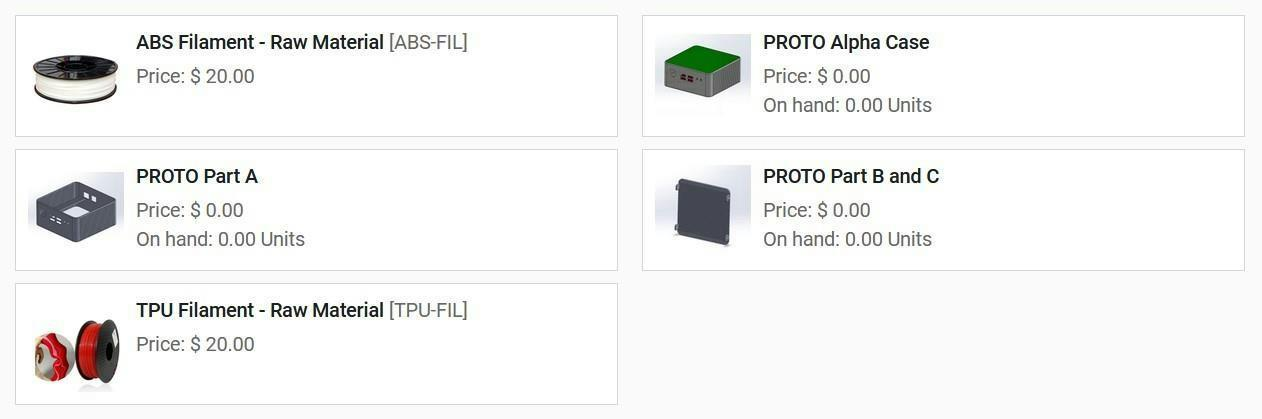
\includegraphics[width=437.85pt,height=144.55pt]{latexImage_0f8dd214cf410e514481d101fb39a864.png}}
\put(503.5,-268.93){\fontsize{9.96}{1}\usefont{T1}{ptm}{m}{n}\selectfont\color{color_29791} }
\put(237.41,-287.53){\fontsize{12}{1}\usefont{T1}{ptm}{b}{n}\selectfont\color{color_29791}圖}
\put(249.41,-287.53){\fontsize{12}{1}\usefont{T1}{ptm}{b}{n}\selectfont\color{color_29791}37}
\put(261.41,-287.53){\fontsize{12}{1}\usefont{T1}{ptm}{b}{n}\selectfont\color{color_29791}原型產品專案圖}
\put(344.71,-287.53){\fontsize{12}{1}\usefont{T1}{ptm}{b}{n}\selectfont\color{color_29791} }
\put(82.944,-319.33){\fontsize{12}{1}\usefont{T1}{ptm}{m}{n}\selectfont\color{color_29791}正}
\put(94.824,-319.33){\fontsize{12}{1}\usefont{T1}{ptm}{m}{n}\selectfont\color{color_29791}如}
\put(106.704,-319.33){\fontsize{12}{1}\usefont{T1}{ptm}{m}{n}\selectfont\color{color_29791}我}
\put(118.584,-319.33){\fontsize{12}{1}\usefont{T1}{ptm}{m}{n}\selectfont\color{color_29791}們}
\put(130.464,-319.33){\fontsize{12}{1}\usefont{T1}{ptm}{m}{n}\selectfont\color{color_29791}之前}
\put(154.344,-319.33){\fontsize{12}{1}\usefont{T1}{ptm}{m}{n}\selectfont\color{color_29791}在}
\put(166.224,-319.33){\fontsize{12}{1}\usefont{T1}{ptm}{m}{n}\selectfont\color{color_29791}第}
\put(178.1,-319.33){\fontsize{12}{1}\usefont{T1}{ptm}{m}{n}\selectfont\color{color_29791} }
\put(184.13,-319.33){\fontsize{12}{1}\usefont{T1}{ptm}{m}{n}\selectfont\color{color_29791}3}
\put(190.13,-319.33){\fontsize{12}{1}\usefont{T1}{ptm}{m}{n}\selectfont\color{color_29791} }
\put(196.13,-319.33){\fontsize{12}{1}\usefont{T1}{ptm}{m}{n}\selectfont\color{color_29791}章中所確定}
\put(256.01,-319.33){\fontsize{12}{1}\usefont{T1}{ptm}{m}{n}\selectfont\color{color_29791}的,該}
\put(291.89,-319.33){\fontsize{12}{1}\usefont{T1}{ptm}{m}{n}\selectfont\color{color_29791}產品}
\put(315.77,-319.33){\fontsize{12}{1}\usefont{T1}{ptm}{m}{n}\selectfont\color{color_29791}將包括}
\put(351.79,-319.33){\fontsize{12}{1}\usefont{T1}{ptm}{m}{n}\selectfont\color{color_29791} }
\put(357.79,-319.33){\fontsize{12}{1}\usefont{T1}{ptm}{m}{n}\selectfont\color{color_29791}A}
\put(366.43,-319.33){\fontsize{12}{1}\usefont{T1}{ptm}{m}{n}\selectfont\color{color_29791} }
\put(372.07,-319.33){\fontsize{12}{1}\usefont{T1}{ptm}{m}{n}\selectfont\color{color_29791}部分、}
\put(408.07,-319.33){\fontsize{12}{1}\usefont{T1}{ptm}{m}{n}\selectfont\color{color_29791}B}
\put(416.11,-319.33){\fontsize{12}{1}\usefont{T1}{ptm}{m}{n}\selectfont\color{color_29791} }
\put(421.99,-319.33){\fontsize{12}{1}\usefont{T1}{ptm}{m}{n}\selectfont\color{color_29791}部}
\put(433.75,-319.33){\fontsize{12}{1}\usefont{T1}{ptm}{m}{n}\selectfont\color{color_29791}分}
\put(445.63,-319.33){\fontsize{12}{1}\usefont{T1}{ptm}{m}{n}\selectfont\color{color_29791}和}
\put(457.54,-319.33){\fontsize{12}{1}\usefont{T1}{ptm}{m}{n}\selectfont\color{color_29791} }
\put(463.54,-319.33){\fontsize{12}{1}\usefont{T1}{ptm}{m}{n}\selectfont\color{color_29791}C}
\put(471.58,-319.33){\fontsize{12}{1}\usefont{T1}{ptm}{m}{n}\selectfont\color{color_29791} }
\put(477.46,-319.33){\fontsize{12}{1}\usefont{T1}{ptm}{m}{n}\selectfont\color{color_29791}部分}
\put(500.98,-319.33){\fontsize{12}{1}\usefont{T1}{ptm}{m}{n}\selectfont\color{color_29791} }
\put(506.86,-319.33){\fontsize{12}{1}\usefont{T1}{ptm}{m}{n}\selectfont\color{color_29791}3}
\put(69.384,-337.21){\fontsize{12}{1}\usefont{T1}{ptm}{m}{n}\selectfont\color{color_29791}部}
\put(81.732,-337.21){\fontsize{12}{1}\usefont{T1}{ptm}{m}{n}\selectfont\color{color_29791}分}
\put(94.08,-337.21){\fontsize{12}{1}\usefont{T1}{ptm}{m}{n}\selectfont\color{color_29791}。}
\put(106.428,-337.21){\fontsize{12}{1}\usefont{T1}{ptm}{m}{n}\selectfont\color{color_29791}這}
\put(118.656,-337.21){\fontsize{12}{1}\usefont{T1}{ptm}{m}{n}\selectfont\color{color_29791}些}
\put(131.004,-337.21){\fontsize{12}{1}\usefont{T1}{ptm}{m}{n}\selectfont\color{color_29791}也}
\put(143.352,-337.21){\fontsize{12}{1}\usefont{T1}{ptm}{m}{n}\selectfont\color{color_29791}需}
\put(155.58,-337.21){\fontsize{12}{1}\usefont{T1}{ptm}{m}{n}\selectfont\color{color_29791}要}
\put(167.928,-337.21){\fontsize{12}{1}\usefont{T1}{ptm}{m}{n}\selectfont\color{color_29791}作}
\put(180.156,-337.21){\fontsize{12}{1}\usefont{T1}{ptm}{m}{n}\selectfont\color{color_29791}為}
\put(192.504,-337.21){\fontsize{12}{1}\usefont{T1}{ptm}{m}{n}\selectfont\color{color_29791}產}
\put(204.852,-337.21){\fontsize{12}{1}\usefont{T1}{ptm}{m}{n}\selectfont\color{color_29791}品}
\put(217.2,-337.21){\fontsize{12}{1}\usefont{T1}{ptm}{m}{n}\selectfont\color{color_29791}進}
\put(229.4279,-337.21){\fontsize{12}{1}\usefont{T1}{ptm}{m}{n}\selectfont\color{color_29791}行}
\put(241.7759,-337.21){\fontsize{12}{1}\usefont{T1}{ptm}{m}{n}\selectfont\color{color_29791}原}
\put(254.1239,-337.21){\fontsize{12}{1}\usefont{T1}{ptm}{m}{n}\selectfont\color{color_29791}型}
\put(266.3519,-337.21){\fontsize{12}{1}\usefont{T1}{ptm}{m}{n}\selectfont\color{color_29791}設}
\put(278.6999,-337.21){\fontsize{12}{1}\usefont{T1}{ptm}{m}{n}\selectfont\color{color_29791}計}
\put(290.9279,-337.21){\fontsize{12}{1}\usefont{T1}{ptm}{m}{n}\selectfont\color{color_29791}和}
\put(303.2759,-337.21){\fontsize{12}{1}\usefont{T1}{ptm}{m}{n}\selectfont\color{color_29791}創}
\put(315.6239,-337.21){\fontsize{12}{1}\usefont{T1}{ptm}{m}{n}\selectfont\color{color_29791}建}
\put(327.9719,-337.21){\fontsize{12}{1}\usefont{T1}{ptm}{m}{n}\selectfont\color{color_29791},}
\put(340.1999,-337.21){\fontsize{12}{1}\usefont{T1}{ptm}{m}{n}\selectfont\color{color_29791}以}
\put(352.5479,-337.21){\fontsize{12}{1}\usefont{T1}{ptm}{m}{n}\selectfont\color{color_29791}便}
\put(364.8959,-337.21){\fontsize{12}{1}\usefont{T1}{ptm}{m}{n}\selectfont\color{color_29791}將}
\put(377.1239,-337.21){\fontsize{12}{1}\usefont{T1}{ptm}{m}{n}\selectfont\color{color_29791}它}
\put(389.4719,-337.21){\fontsize{12}{1}\usefont{T1}{ptm}{m}{n}\selectfont\color{color_29791}們}
\put(401.6999,-337.21){\fontsize{12}{1}\usefont{T1}{ptm}{m}{n}\selectfont\color{color_29791}添}
\put(414.0479,-337.21){\fontsize{12}{1}\usefont{T1}{ptm}{m}{n}\selectfont\color{color_29791}加}
\put(426.3958,-337.21){\fontsize{12}{1}\usefont{T1}{ptm}{m}{n}\selectfont\color{color_29791}到}
\put(439.18,-337.21){\fontsize{12}{1}\usefont{T1}{ptm}{m}{n}\selectfont\color{color_29791}P}
\put(445.78,-337.21){\fontsize{12}{1}\usefont{T1}{ptm}{m}{n}\selectfont\color{color_29791}R}
\put(453.808,-337.21){\fontsize{12}{1}\usefont{T1}{ptm}{m}{n}\selectfont\color{color_29791}OT}
\put(469.768,-337.21){\fontsize{12}{1}\usefont{T1}{ptm}{m}{n}\selectfont\color{color_29791}O }
\put(483.556,-337.21){\fontsize{12}{1}\usefont{T1}{ptm}{m}{n}\selectfont\color{color_29791}Alpha}
\put(512.7159,-337.21){\fontsize{12}{1}\usefont{T1}{ptm}{m}{n}\selectfont\color{color_29791} }
\put(69.384,-355.09){\fontsize{12}{1}\usefont{T1}{ptm}{m}{n}\selectfont\color{color_29791}C}
\put(77.412,-355.09){\fontsize{12}{1}\usefont{T1}{ptm}{m}{n}\selectfont\color{color_29791}a}
\put(82.692,-355.09){\fontsize{12}{1}\usefont{T1}{ptm}{m}{n}\selectfont\color{color_29791}se}
\put(92.66,-355.09){\fontsize{12}{1}\usefont{T1}{ptm}{m}{n}\selectfont\color{color_29791}的物料清單中。最後,決定使用特定的塑料長絲(}
\put(356.71,-355.09){\fontsize{12}{1}\usefont{T1}{ptm}{m}{n}\selectfont\color{color_29791}參見第}
\put(391.63,-355.09){\fontsize{12}{1}\usefont{T1}{ptm}{m}{n}\selectfont\color{color_29791} }
\put(397.27,-355.09){\fontsize{12}{1}\usefont{T1}{ptm}{m}{n}\selectfont\color{color_29791}4.1.1}
\put(421.27,-355.09){\fontsize{12}{1}\usefont{T1}{ptm}{m}{n}\selectfont\color{color_29791} }
\put(424.75,-355.09){\fontsize{12}{1}\usefont{T1}{ptm}{m}{n}\selectfont\color{color_29791}節)}
\put(448.78,-355.09){\fontsize{12}{1}\usefont{T1}{ptm}{m}{n}\selectfont\color{color_29791}進行}
\put(473.98,-355.09){\fontsize{12}{1}\usefont{T1}{ptm}{m}{n}\selectfont\color{color_29791}P}
\put(480.58,-355.09){\fontsize{12}{1}\usefont{T1}{ptm}{m}{n}\selectfont\color{color_29791}R}
\put(488.5,-355.09){\fontsize{12}{1}\usefont{T1}{ptm}{m}{n}\selectfont\color{color_29791}O}
\put(497.02,-355.09){\fontsize{12}{1}\usefont{T1}{ptm}{m}{n}\selectfont\color{color_29791}T}
\put(504.22,-355.09){\fontsize{12}{1}\usefont{T1}{ptm}{m}{n}\selectfont\color{color_29791}O}
\put(512.7401,-355.09){\fontsize{12}{1}\usefont{T1}{ptm}{m}{n}\selectfont\color{color_29791} }
\put(69.384,-372.97){\fontsize{12}{1}\usefont{T1}{ptm}{m}{n}\selectfont\color{color_29791}A}
\put(78.024,-372.97){\fontsize{12}{1}\usefont{T1}{ptm}{m}{n}\selectfont\color{color_29791} }
\put(80.304,-372.97){\fontsize{12}{1}\usefont{T1}{ptm}{m}{n}\selectfont\color{color_29791}部分和}
\put(114.14,-372.97){\fontsize{12}{1}\usefont{T1}{ptm}{m}{n}\selectfont\color{color_29791} }
\put(119.42,-372.97){\fontsize{12}{1}\usefont{T1}{ptm}{m}{n}\selectfont\color{color_29791}P}
\put(126.128,-372.97){\fontsize{12}{1}\usefont{T1}{ptm}{m}{n}\selectfont\color{color_29791}R}
\put(134.156,-372.97){\fontsize{12}{1}\usefont{T1}{ptm}{m}{n}\selectfont\color{color_29791}OT}
\put(150.116,-372.97){\fontsize{12}{1}\usefont{T1}{ptm}{m}{n}\selectfont\color{color_29791}O B}
\put(169.82,-372.97){\fontsize{12}{1}\usefont{T1}{ptm}{m}{n}\selectfont\color{color_29791} }
\put(172.7,-372.97){\fontsize{12}{1}\usefont{T1}{ptm}{m}{n}\selectfont\color{color_29791}部}
\put(183.86,-372.97){\fontsize{12}{1}\usefont{T1}{ptm}{m}{n}\selectfont\color{color_29791}分}
\put(195.14,-372.97){\fontsize{12}{1}\usefont{T1}{ptm}{m}{n}\selectfont\color{color_29791}和}
\put(206.45,-372.97){\fontsize{12}{1}\usefont{T1}{ptm}{m}{n}\selectfont\color{color_29791} }
\put(211.73,-372.97){\fontsize{12}{1}\usefont{T1}{ptm}{m}{n}\selectfont\color{color_29791}C }
\put(222.77,-372.97){\fontsize{12}{1}\usefont{T1}{ptm}{m}{n}\selectfont\color{color_29791}部}
\put(233.93,-372.97){\fontsize{12}{1}\usefont{T1}{ptm}{m}{n}\selectfont\color{color_29791}分}
\put(245.21,-372.97){\fontsize{12}{1}\usefont{T1}{ptm}{m}{n}\selectfont\color{color_29791}的}
\put(256.49,-372.97){\fontsize{12}{1}\usefont{T1}{ptm}{m}{n}\selectfont\color{color_29791} }
\put(261.77,-372.97){\fontsize{12}{1}\usefont{T1}{ptm}{m}{n}\selectfont\color{color_29791}3D }
\put(279.41,-372.97){\fontsize{12}{1}\usefont{T1}{ptm}{m}{n}\selectfont\color{color_29791}列印}
\put(303.29,-372.97){\fontsize{12}{1}\usefont{T1}{ptm}{m}{n}\selectfont\color{color_29791},這些也需要作為產品添加(}
\put(459.34,-372.97){\fontsize{12}{1}\usefont{T1}{ptm}{m}{n}\selectfont\color{color_29791}圖}
\put(469.78,-372.97){\fontsize{12}{1}\usefont{T1}{ptm}{m}{n}\selectfont\color{color_29791} }
\put(474.22,-372.97){\fontsize{12}{1}\usefont{T1}{ptm}{m}{n}\selectfont\color{color_29791}38}
\put(486.22,-372.97){\fontsize{12}{1}\usefont{T1}{ptm}{m}{n}\selectfont\color{color_29791})。}
\put(510.34,-372.97){\fontsize{12}{1}\usefont{T1}{ptm}{m}{n}\selectfont\color{color_29791} }
\put(63.024,-390.37){\fontsize{9.96}{1}\usefont{T1}{ptm}{m}{n}\selectfont\color{color_29791} }
\put(216.17,-554.19){\fontsize{12}{1}\usefont{T1}{ptm}{b}{n}\selectfont\color{color_29791}圖}
\put(228.17,-554.19){\fontsize{12}{1}\usefont{T1}{ptm}{b}{n}\selectfont\color{color_29791} }
\put(231.17,-554.19){\fontsize{12}{1}\usefont{T1}{ptm}{b}{n}\selectfont\color{color_29791}38}
\put(243.17,-554.19){\fontsize{12}{1}\usefont{T1}{ptm}{b}{n}\selectfont\color{color_29791} }
\put(246.05,-554.19){\fontsize{12}{1}\usefont{T1}{ptm}{b}{n}\selectfont\color{color_29791}原型的產品類}
\put(317.93,-554.19){\fontsize{12}{1}\usefont{T1}{ptm}{b}{n}\selectfont\color{color_29791}專}
\put(329.81,-554.19){\fontsize{12}{1}\usefont{T1}{ptm}{b}{n}\selectfont\color{color_29791}案概述}
\put(365.71,-554.19){\fontsize{12}{1}\usefont{T1}{ptm}{b}{n}\selectfont\color{color_29791} }
\put(82.944,-584.7){\fontsize{12}{1}\usefont{T1}{ptm}{m}{n}\selectfont\color{color_29791}至此,}
\put(118.58,-584.7){\fontsize{12}{1}\usefont{T1}{ptm}{m}{n}\selectfont\color{color_29791}A}
\put(127.1,-584.7){\fontsize{12}{1}\usefont{T1}{ptm}{m}{n}\selectfont\color{color_29791}l}
\put(130.34,-584.7){\fontsize{12}{1}\usefont{T1}{ptm}{m}{n}\selectfont\color{color_29791}p}
\put(136.22,-584.7){\fontsize{12}{1}\usefont{T1}{ptm}{m}{n}\selectfont\color{color_29791}ha}
\put(147.5,-584.7){\fontsize{12}{1}\usefont{T1}{ptm}{m}{n}\selectfont\color{color_29791} }
\put(69.384,-602.7){\fontsize{12}{1}\usefont{T1}{ptm}{m}{n}\selectfont\color{color_29791}C}
\put(77.304,-602.7){\fontsize{12}{1}\usefont{T1}{ptm}{m}{n}\selectfont\color{color_29791}a}
\put(82.464,-602.7){\fontsize{12}{1}\usefont{T1}{ptm}{m}{n}\selectfont\color{color_29791}s}
\put(87.024,-602.7){\fontsize{12}{1}\usefont{T1}{ptm}{m}{n}\selectfont\color{color_29791}e}
\put(92.18,-602.7){\fontsize{12}{1}\usefont{T1}{ptm}{m}{n}\selectfont\color{color_29791}原}
\put(104.06,-602.7){\fontsize{12}{1}\usefont{T1}{ptm}{m}{n}\selectfont\color{color_29791}型製}
\put(127.94,-602.7){\fontsize{12}{1}\usefont{T1}{ptm}{m}{n}\selectfont\color{color_29791}作}
\put(139.82,-602.7){\fontsize{12}{1}\usefont{T1}{ptm}{m}{n}\selectfont\color{color_29791}的}
\put(151.7,-602.7){\fontsize{12}{1}\usefont{T1}{ptm}{m}{n}\selectfont\color{color_29791}相}
\put(163.58,-602.7){\fontsize{12}{1}\usefont{T1}{ptm}{m}{n}\selectfont\color{color_29791}關}
\put(175.46,-602.7){\fontsize{12}{1}\usefont{T1}{ptm}{m}{n}\selectfont\color{color_29791}產品}
\put(199.34,-602.7){\fontsize{12}{1}\usefont{T1}{ptm}{m}{n}\selectfont\color{color_29791}專}
\put(211.22,-602.7){\fontsize{12}{1}\usefont{T1}{ptm}{m}{n}\selectfont\color{color_29791}案}
\put(223.1,-602.7){\fontsize{12}{1}\usefont{T1}{ptm}{m}{n}\selectfont\color{color_29791}已}
\put(234.98,-602.7){\fontsize{12}{1}\usefont{T1}{ptm}{m}{n}\selectfont\color{color_29791}經}
\put(246.86,-602.7){\fontsize{12}{1}\usefont{T1}{ptm}{m}{n}\selectfont\color{color_29791}完}
\put(258.7401,-602.7){\fontsize{12}{1}\usefont{T1}{ptm}{m}{n}\selectfont\color{color_29791}成}
\put(270.6201,-602.7){\fontsize{12}{1}\usefont{T1}{ptm}{m}{n}\selectfont\color{color_29791},這}
\put(294.5001,-602.7){\fontsize{12}{1}\usefont{T1}{ptm}{m}{n}\selectfont\color{color_29791}使得}
\put(318.3801,-602.7){\fontsize{12}{1}\usefont{T1}{ptm}{m}{n}\selectfont\color{color_29791}創}
\put(330.2601,-602.7){\fontsize{12}{1}\usefont{T1}{ptm}{m}{n}\selectfont\color{color_29791}建}
\put(342.1401,-602.7){\fontsize{12}{1}\usefont{T1}{ptm}{m}{n}\selectfont\color{color_29791}其}
\put(354.0201,-602.7){\fontsize{12}{1}\usefont{T1}{ptm}{m}{n}\selectfont\color{color_29791}相}
\put(365.9001,-602.7){\fontsize{12}{1}\usefont{T1}{ptm}{m}{n}\selectfont\color{color_29791}關}
\put(377.83,-602.7){\fontsize{12}{1}\usefont{T1}{ptm}{m}{n}\selectfont\color{color_29791}B}
\put(385.75,-602.7){\fontsize{12}{1}\usefont{T1}{ptm}{m}{n}\selectfont\color{color_29791}O}
\put(394.27,-602.7){\fontsize{12}{1}\usefont{T1}{ptm}{m}{n}\selectfont\color{color_29791}M}
\put(404.95,-602.7){\fontsize{12}{1}\usefont{T1}{ptm}{m}{n}\selectfont\color{color_29791}成}
\put(416.83,-602.7){\fontsize{12}{1}\usefont{T1}{ptm}{m}{n}\selectfont\color{color_29791}為可}
\put(440.71,-602.7){\fontsize{12}{1}\usefont{T1}{ptm}{m}{n}\selectfont\color{color_29791}能}
\put(452.59,-602.7){\fontsize{12}{1}\usefont{T1}{ptm}{m}{n}\selectfont\color{color_29791}。}
\put(464.47,-602.7){\fontsize{12}{1}\usefont{T1}{ptm}{m}{n}\selectfont\color{color_29791}其}
\put(476.35,-602.7){\fontsize{12}{1}\usefont{T1}{ptm}{m}{n}\selectfont\color{color_29791}中}
\put(488.23,-602.7){\fontsize{12}{1}\usefont{T1}{ptm}{m}{n}\selectfont\color{color_29791}有}
\put(500.14,-602.7){\fontsize{12}{1}\usefont{T1}{ptm}{m}{n}\selectfont\color{color_29791} }
\put(506.02,-602.7){\fontsize{12}{1}\usefont{T1}{ptm}{m}{n}\selectfont\color{color_29791}3}
\put(511.66,-602.7){\fontsize{12}{1}\usefont{T1}{ptm}{m}{n}\selectfont\color{color_29791} }
\put(69.384,-620.46){\fontsize{12}{1}\usefont{T1}{ptm}{m}{n}\selectfont\color{color_29791}個,它們遵循(}
\put(152.66,-620.46){\fontsize{12}{1}\usefont{T1}{ptm}{m}{n}\selectfont\color{color_29791}圖}
\put(163.7,-620.46){\fontsize{12}{1}\usefont{T1}{ptm}{m}{n}\selectfont\color{color_29791} }
\put(168.74,-620.46){\fontsize{12}{1}\usefont{T1}{ptm}{m}{n}\selectfont\color{color_29791}39}
\put(180.77,-620.46){\fontsize{12}{1}\usefont{T1}{ptm}{m}{n}\selectfont\color{color_29791})}
\put(192.65,-620.46){\fontsize{12}{1}\usefont{T1}{ptm}{m}{n}\selectfont\color{color_29791}中}
\put(204.41,-620.46){\fontsize{12}{1}\usefont{T1}{ptm}{m}{n}\selectfont\color{color_29791}的}
\put(216.17,-620.46){\fontsize{12}{1}\usefont{T1}{ptm}{m}{n}\selectfont\color{color_29791}結}
\put(228.05,-620.46){\fontsize{12}{1}\usefont{T1}{ptm}{m}{n}\selectfont\color{color_29791}構}
\put(239.81,-620.46){\fontsize{12}{1}\usefont{T1}{ptm}{m}{n}\selectfont\color{color_29791}:}
\put(251.69,-620.46){\fontsize{12}{1}\usefont{T1}{ptm}{m}{n}\selectfont\color{color_29791} }
\put(73.75,-268.85){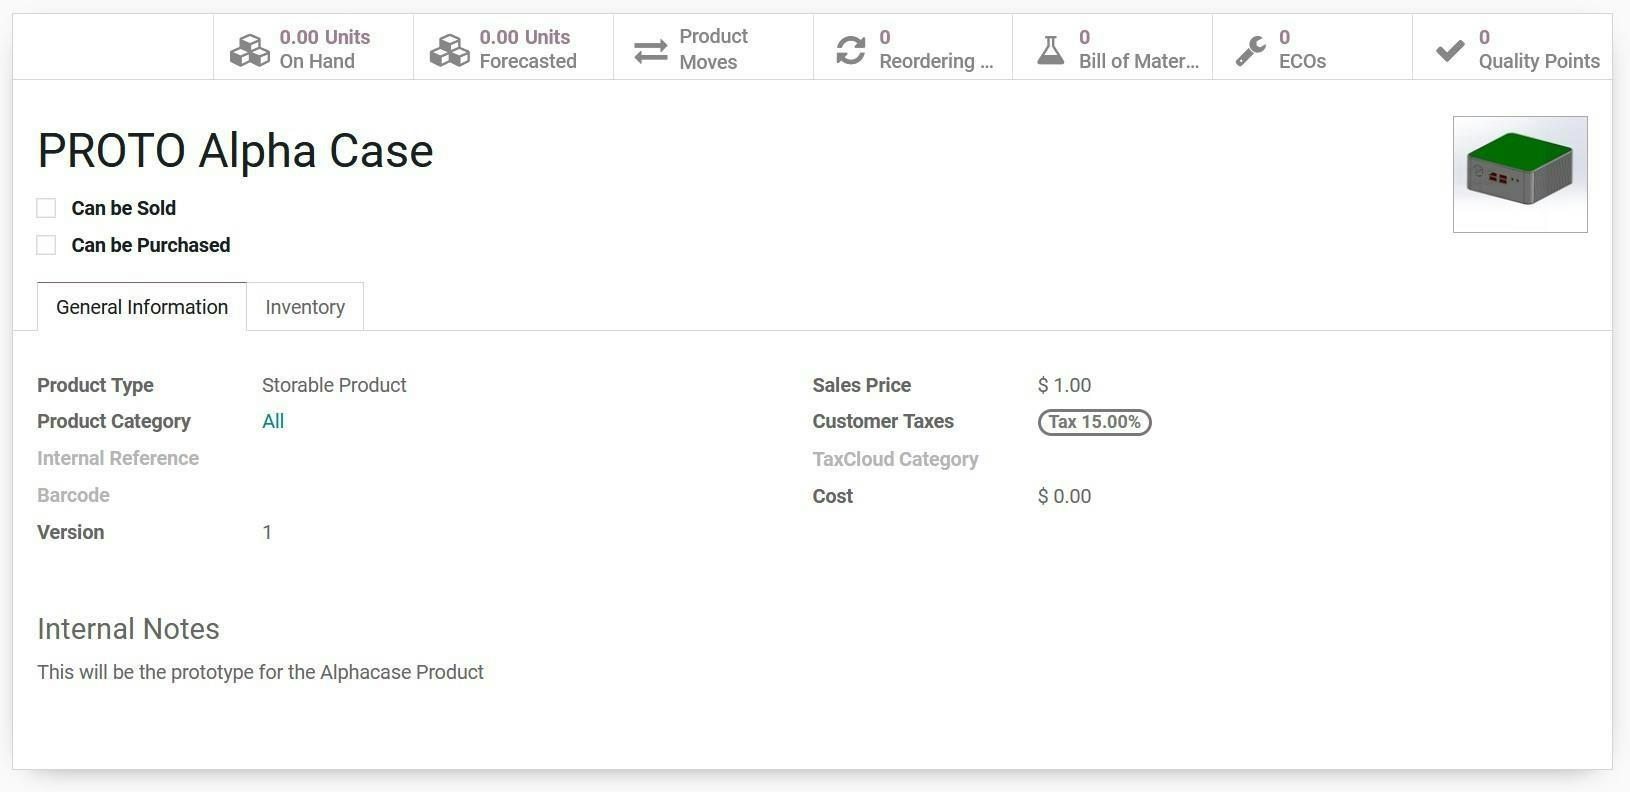
\includegraphics[width=429.55pt,height=207.85pt]{latexImage_76deb0f073e12e73e0f5d332f6905bbd.png}}
\end{picture}
\newpage
\begin{tikzpicture}[overlay]\path(0pt,0pt);\end{tikzpicture}
\begin{picture}(-5,0)(2.5,0)
\put(500.26,-727.616){\fontsize{12}{1}\usefont{T1}{ptm}{m}{n}\selectfont\color{color_29791}44}
\put(511.78,-727.616){\fontsize{12}{1}\usefont{T1}{ptm}{m}{n}\selectfont\color{color_29791} }
\put(63.024,-726.896){\fontsize{9.96}{1}\usefont{T1}{ptm}{m}{n}\selectfont\color{color_29791} }
\put(70.05,-654.9){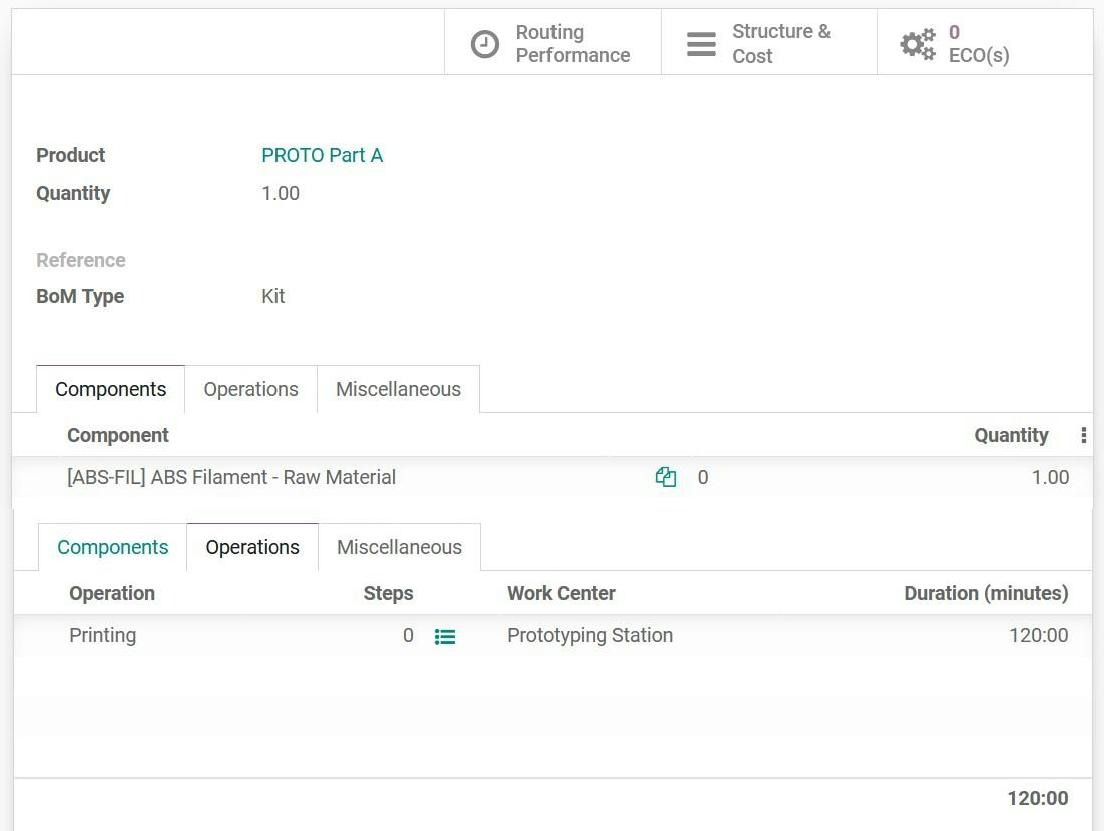
\includegraphics[width=438.98pt,height=330.3pt]{latexImage_0e3a5bd79fba480ddc364635305b19d5.png}}
\put(517.9,-236.26){\fontsize{9.96}{1}\usefont{T1}{ptm}{m}{n}\selectfont\color{color_29791} }
\put(222.89,-253.69){\fontsize{12}{1}\usefont{T1}{ptm}{b}{n}\selectfont\color{color_29791}圖}
\put(234.89,-253.69){\fontsize{12}{1}\usefont{T1}{ptm}{b}{n}\selectfont\color{color_29791} }
\put(237.89,-253.69){\fontsize{12}{1}\usefont{T1}{ptm}{b}{n}\selectfont\color{color_29791}39}
\put(249.89,-253.69){\fontsize{12}{1}\usefont{T1}{ptm}{b}{n}\selectfont\color{color_29791} }
\put(252.77,-253.69){\fontsize{12}{1}\usefont{T1}{ptm}{b}{n}\selectfont\color{color_29791}原型製作的}
\put(312.79,-253.69){\fontsize{12}{1}\usefont{T1}{ptm}{b}{n}\selectfont\color{color_29791} }
\put(315.79,-253.69){\fontsize{12}{1}\usefont{T1}{ptm}{b}{n}\selectfont\color{color_29791}B}
\put(323.818,-253.69){\fontsize{12}{1}\usefont{T1}{ptm}{b}{n}\selectfont\color{color_29791}OM}
\put(344.566,-253.69){\fontsize{12}{1}\usefont{T1}{ptm}{b}{n}\selectfont\color{color_29791} }
\put(347.59,-253.69){\fontsize{12}{1}\usefont{T1}{ptm}{b}{n}\selectfont\color{color_29791}圖}
\put(359.11,-253.69){\fontsize{12}{1}\usefont{T1}{ptm}{b}{n}\selectfont\color{color_29791} }
\put(82.944,-285.49){\fontsize{12}{1}\usefont{T1}{ptm}{m}{n}\selectfont\color{color_29791}值得一提的是,}
\put(166.22,-285.49){\fontsize{12}{1}\usefont{T1}{ptm}{m}{n}\selectfont\color{color_29791}O}
\put(174.74,-285.49){\fontsize{12}{1}\usefont{T1}{ptm}{m}{n}\selectfont\color{color_29791}d}
\put(180.62,-285.49){\fontsize{12}{1}\usefont{T1}{ptm}{m}{n}\selectfont\color{color_29791}o}
\put(186.5,-285.49){\fontsize{12}{1}\usefont{T1}{ptm}{m}{n}\selectfont\color{color_29791}o}
\put(192.41,-285.49){\fontsize{12}{1}\usefont{T1}{ptm}{m}{n}\selectfont\color{color_29791}在專}
\put(216.29,-285.49){\fontsize{12}{1}\usefont{T1}{ptm}{m}{n}\selectfont\color{color_29791}案}
\put(228.17,-285.49){\fontsize{12}{1}\usefont{T1}{ptm}{m}{n}\selectfont\color{color_29791}上}
\put(240.05,-285.49){\fontsize{12}{1}\usefont{T1}{ptm}{m}{n}\selectfont\color{color_29791}使}
\put(251.93,-285.49){\fontsize{12}{1}\usefont{T1}{ptm}{m}{n}\selectfont\color{color_29791}用}
\put(263.81,-285.49){\fontsize{12}{1}\usefont{T1}{ptm}{m}{n}\selectfont\color{color_29791}了}
\put(275.69,-285.49){\fontsize{12}{1}\usefont{T1}{ptm}{m}{n}\selectfont\color{color_29791}套}
\put(287.57,-285.49){\fontsize{12}{1}\usefont{T1}{ptm}{m}{n}\selectfont\color{color_29791}件選}
\put(311.45,-285.49){\fontsize{12}{1}\usefont{T1}{ptm}{m}{n}\selectfont\color{color_29791}項(}
\put(335.33,-285.49){\fontsize{12}{1}\usefont{T1}{ptm}{m}{n}\selectfont\color{color_29791}圖}
\put(347.23,-285.49){\fontsize{12}{1}\usefont{T1}{ptm}{m}{n}\selectfont\color{color_29791}40}
\put(358.99,-285.49){\fontsize{12}{1}\usefont{T1}{ptm}{m}{n}\selectfont\color{color_29791})}
\put(370.87,-285.49){\fontsize{12}{1}\usefont{T1}{ptm}{m}{n}\selectfont\color{color_29791}來}
\put(382.75,-285.49){\fontsize{12}{1}\usefont{T1}{ptm}{m}{n}\selectfont\color{color_29791}推}
\put(394.63,-285.49){\fontsize{12}{1}\usefont{T1}{ptm}{m}{n}\selectfont\color{color_29791}斷該}
\put(418.51,-285.49){\fontsize{12}{1}\usefont{T1}{ptm}{m}{n}\selectfont\color{color_29791}產}
\put(430.39,-285.49){\fontsize{12}{1}\usefont{T1}{ptm}{m}{n}\selectfont\color{color_29791}品是}
\put(454.27,-285.49){\fontsize{12}{1}\usefont{T1}{ptm}{m}{n}\selectfont\color{color_29791}另}
\put(466.15,-285.49){\fontsize{12}{1}\usefont{T1}{ptm}{m}{n}\selectfont\color{color_29791}一}
\put(478.03,-285.49){\fontsize{12}{1}\usefont{T1}{ptm}{m}{n}\selectfont\color{color_29791}個}
\put(489.91,-285.49){\fontsize{12}{1}\usefont{T1}{ptm}{m}{n}\selectfont\color{color_29791}產}
\put(69.384,-303.49){\fontsize{12}{1}\usefont{T1}{ptm}{m}{n}\selectfont\color{color_29791}品的元件。這非常}
\put(164.532,-303.49){\fontsize{12}{1}\usefont{T1}{ptm}{m}{n}\selectfont\color{color_29791}有趣}
\put(188.4,-303.49){\fontsize{12}{1}\usefont{T1}{ptm}{m}{n}\selectfont\color{color_29791},因為它會自動在}
\put(283.548,-303.49){\fontsize{12}{1}\usefont{T1}{ptm}{m}{n}\selectfont\color{color_29791}生產}
\put(307.416,-303.49){\fontsize{12}{1}\usefont{T1}{ptm}{m}{n}\selectfont\color{color_29791}產品項之間創建依}
\put(402.564,-303.49){\fontsize{12}{1}\usefont{T1}{ptm}{m}{n}\selectfont\color{color_29791}賴關}
\put(426.432,-303.49){\fontsize{12}{1}\usefont{T1}{ptm}{m}{n}\selectfont\color{color_29791}係。}
\put(450.34,-303.49){\fontsize{12}{1}\usefont{T1}{ptm}{m}{n}\selectfont\color{color_29791} }
\put(63.024,-320.65){\fontsize{9.96}{1}\usefont{T1}{ptm}{m}{n}\selectfont\color{color_29791} }
\put(193.61,-672.78){\fontsize{12}{1}\usefont{T1}{ptm}{b}{n}\selectfont\color{color_29791}圖}
\put(205.61,-672.78){\fontsize{12}{1}\usefont{T1}{ptm}{b}{n}\selectfont\color{color_29791} }
\put(208.61,-672.78){\fontsize{12}{1}\usefont{T1}{ptm}{b}{n}\selectfont\color{color_29791}40}
\put(220.61,-672.78){\fontsize{12}{1}\usefont{T1}{ptm}{b}{n}\selectfont\color{color_29791} }
\put(223.49,-672.78){\fontsize{12}{1}\usefont{T1}{ptm}{b}{n}\selectfont\color{color_29791}原型產品}
\put(271.49,-672.78){\fontsize{12}{1}\usefont{T1}{ptm}{b}{n}\selectfont\color{color_29791} }
\put(274.49,-672.78){\fontsize{12}{1}\usefont{T1}{ptm}{b}{n}\selectfont\color{color_29791}B}
\put(282.518,-672.78){\fontsize{12}{1}\usefont{T1}{ptm}{b}{n}\selectfont\color{color_29791}OM}
\put(303.17,-672.78){\fontsize{12}{1}\usefont{T1}{ptm}{b}{n}\selectfont\color{color_29791} }
\put(306.05,-672.78){\fontsize{12}{1}\usefont{T1}{ptm}{b}{n}\selectfont\color{color_29791}影像(}
\put(342.07,-672.78){\fontsize{12}{1}\usefont{T1}{ptm}{b}{n}\selectfont\color{color_29791}A}
\put(350.71,-672.78){\fontsize{12}{1}\usefont{T1}{ptm}{b}{n}\selectfont\color{color_29791} }
\put(352.99,-672.78){\fontsize{12}{1}\usefont{T1}{ptm}{b}{n}\selectfont\color{color_29791}部分}
\put(376.99,-672.78){\fontsize{12}{1}\usefont{T1}{ptm}{b}{n}\selectfont\color{color_29791})}
\put(388.51,-672.78){\fontsize{12}{1}\usefont{T1}{ptm}{b}{n}\selectfont\color{color_29791} }
\put(79.55,-236.25){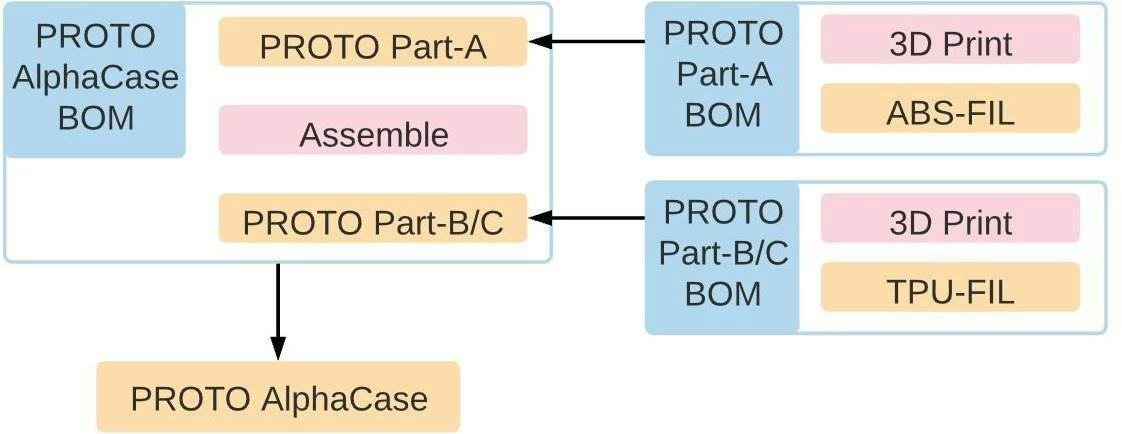
\includegraphics[width=438.35pt,height=169.25pt]{latexImage_0158fdfd8b191a9666196aba45a10ab5.png}}
\end{picture}
\newpage
\begin{tikzpicture}[overlay]\path(0pt,0pt);\end{tikzpicture}
\begin{picture}(-5,0)(2.5,0)
\put(500.26,-727.616){\fontsize{12}{1}\usefont{T1}{ptm}{m}{n}\selectfont\color{color_29791}45}
\put(511.78,-727.616){\fontsize{12}{1}\usefont{T1}{ptm}{m}{n}\selectfont\color{color_29791} }
\put(63.024,-726.896){\fontsize{9.96}{1}\usefont{T1}{ptm}{m}{n}\selectfont\color{color_29791} }
\put(73.75,-513.99){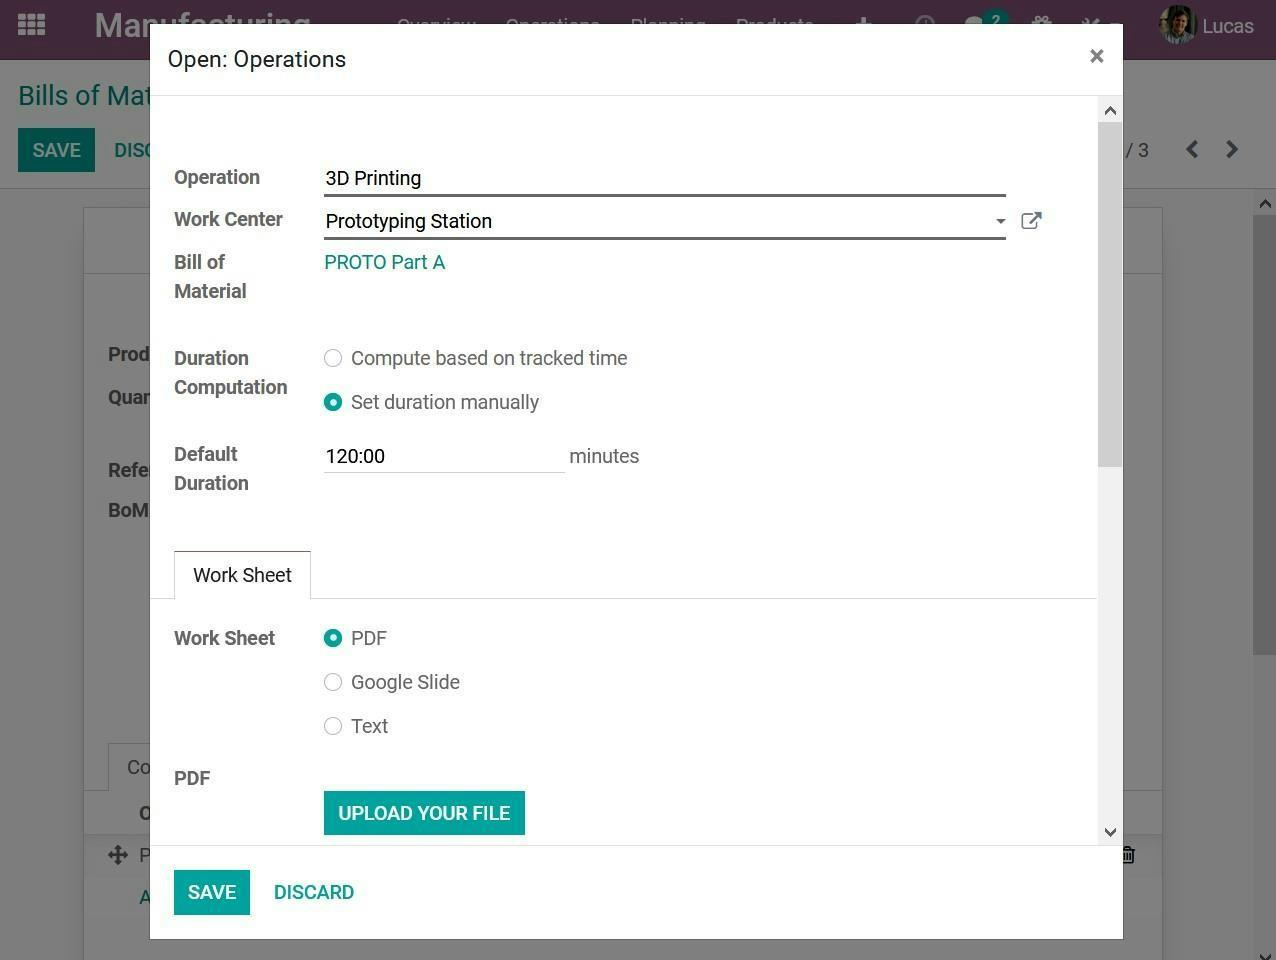
\includegraphics[width=440.25pt,height=331.19pt]{latexImage_e8bca1400249ff78e1d040c042836c13.png}}
\put(73.25,-689.3){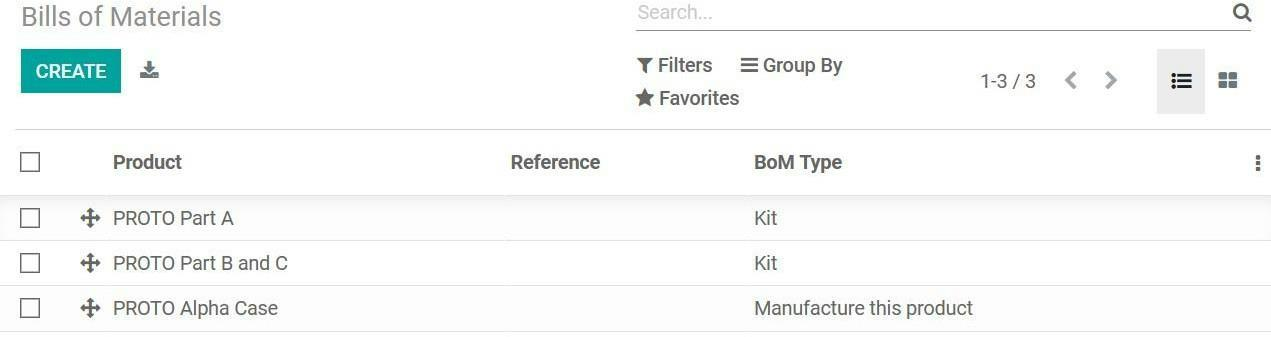
\includegraphics[width=428.89pt,height=113.7pt]{latexImage_b0905651ddd07adaa4b9183c51b3ed1d.png}}
\put(85.94,-72.56){\fontsize{12}{1}\usefont{T1}{ptm}{m}{n}\selectfont\color{color_29791}正如讀者所看到的(圖}
\put(205.97,-72.56){\fontsize{12}{1}\usefont{T1}{ptm}{m}{n}\selectfont\color{color_29791} }
\put(309.55,-72.56){\fontsize{12}{1}\usefont{T1}{ptm}{m}{n}\selectfont\color{color_29791}41}
\put(321.55,-72.56){\fontsize{12}{1}\usefont{T1}{ptm}{m}{n}\selectfont\color{color_29791}),在製作}
\put(381.55,-72.56){\fontsize{12}{1}\usefont{T1}{ptm}{m}{n}\selectfont\color{color_29791} }
\put(485.26,-72.56){\fontsize{12}{1}\usefont{T1}{ptm}{m}{n}\selectfont\color{color_29791}B}
\put(492.94,-72.56){\fontsize{12}{1}\usefont{T1}{ptm}{m}{n}\selectfont\color{color_29791}O}
\put(501.34,-72.56){\fontsize{12}{1}\usefont{T1}{ptm}{m}{n}\selectfont\color{color_29791}M}
\put(69.384,-90.21997){\fontsize{12}{1}\usefont{T1}{ptm}{m}{n}\selectfont\color{color_29791}時}
\put(81.384,-90.21997){\fontsize{12}{1}\usefont{T1}{ptm}{m}{n}\selectfont\color{color_29791},}
\put(93.38,-90.21997){\fontsize{12}{1}\usefont{T1}{ptm}{m}{n}\selectfont\color{color_29791}創建製造過程所需的特定操作專案並指定其工作中心非常簡}
\put(405.43,-90.21997){\fontsize{12}{1}\usefont{T1}{ptm}{m}{n}\selectfont\color{color_29791}單}
\put(417.43,-90.21997){\fontsize{12}{1}\usefont{T1}{ptm}{m}{n}\selectfont\color{color_29791}。}
\put(429.43,-90.21997){\fontsize{12}{1}\usefont{T1}{ptm}{m}{n}\selectfont\color{color_29791}Odoo}
\put(456.1,-90.21997){\fontsize{12}{1}\usefont{T1}{ptm}{m}{n}\selectfont\color{color_29791}中}
\put(468.1,-90.21997){\fontsize{12}{1}\usefont{T1}{ptm}{m}{n}\selectfont\color{color_29791}M}
\put(478.78,-90.21997){\fontsize{12}{1}\usefont{T1}{ptm}{m}{n}\selectfont\color{color_29791}E}
\put(486.1,-90.21997){\fontsize{12}{1}\usefont{T1}{ptm}{m}{n}\selectfont\color{color_29791}S}
\put(492.82,-90.21997){\fontsize{12}{1}\usefont{T1}{ptm}{m}{n}\selectfont\color{color_29791}的}
\put(69.384,-107.86){\fontsize{12}{1}\usefont{T1}{ptm}{m}{n}\selectfont\color{color_29791}最佳功能之一是能夠根據預設持續時間跟蹤操作時間。這可以根據跟蹤時間動態更}
\put(69.384,-125.62){\fontsize{12}{1}\usefont{T1}{ptm}{m}{n}\selectfont\color{color_29791}改或手動設}
\put(129.38,-125.62){\fontsize{12}{1}\usefont{T1}{ptm}{m}{n}\selectfont\color{color_29791}置}
\put(141.38,-125.62){\fontsize{12}{1}\usefont{T1}{ptm}{m}{n}\selectfont\color{color_29791}。}
\put(153.38,-125.62){\fontsize{12}{1}\usefont{T1}{ptm}{m}{n}\selectfont\color{color_29791} }
\put(69.384,-143.62){\fontsize{12}{1}\usefont{T1}{ptm}{m}{n}\selectfont\color{color_29791}同樣在操作項中,}
\put(164.532,-143.62){\fontsize{12}{1}\usefont{T1}{ptm}{m}{n}\selectfont\color{color_29791}我們}
\put(188.4,-143.62){\fontsize{12}{1}\usefont{T1}{ptm}{m}{n}\selectfont\color{color_29791}可以為操作添加指}
\put(283.548,-143.62){\fontsize{12}{1}\usefont{T1}{ptm}{m}{n}\selectfont\color{color_29791}令檔}
\put(307.416,-143.62){\fontsize{12}{1}\usefont{T1}{ptm}{m}{n}\selectfont\color{color_29791}。儘管它僅限於}
\put(390.67,-143.62){\fontsize{12}{1}\usefont{T1}{ptm}{m}{n}\selectfont\color{color_29791}P}
\put(397.27,-143.62){\fontsize{12}{1}\usefont{T1}{ptm}{m}{n}\selectfont\color{color_29791}DF}
\put(412.39,-143.62){\fontsize{12}{1}\usefont{T1}{ptm}{m}{n}\selectfont\color{color_29791}文本}
\put(436.27,-143.62){\fontsize{12}{1}\usefont{T1}{ptm}{m}{n}\selectfont\color{color_29791}或}
\put(448.15,-143.62){\fontsize{12}{1}\usefont{T1}{ptm}{m}{n}\selectfont\color{color_29791}指}
\put(460.03,-143.62){\fontsize{12}{1}\usefont{T1}{ptm}{m}{n}\selectfont\color{color_29791}向}
\put(471.91,-143.62){\fontsize{12}{1}\usefont{T1}{ptm}{m}{n}\selectfont\color{color_29791}谷}
\put(483.79,-143.62){\fontsize{12}{1}\usefont{T1}{ptm}{m}{n}\selectfont\color{color_29791}歌}
\put(495.67,-143.62){\fontsize{12}{1}\usefont{T1}{ptm}{m}{n}\selectfont\color{color_29791}幻}
\put(507.58,-143.62){\fontsize{12}{1}\usefont{T1}{ptm}{m}{n}\selectfont\color{color_29791} }
\put(69.384,-161.62){\fontsize{12}{1}\usefont{T1}{ptm}{m}{n}\selectfont\color{color_29791}燈片文件的連結,}
\put(164.532,-161.62){\fontsize{12}{1}\usefont{T1}{ptm}{m}{n}\selectfont\color{color_29791}但這}
\put(188.4,-161.62){\fontsize{12}{1}\usefont{T1}{ptm}{m}{n}\selectfont\color{color_29791}是}
\put(200.33,-161.62){\fontsize{12}{1}\usefont{T1}{ptm}{m}{n}\selectfont\color{color_29791}O}
\put(208.85,-161.62){\fontsize{12}{1}\usefont{T1}{ptm}{m}{n}\selectfont\color{color_29791}d}
\put(214.73,-161.62){\fontsize{12}{1}\usefont{T1}{ptm}{m}{n}\selectfont\color{color_29791}o}
\put(220.61,-161.62){\fontsize{12}{1}\usefont{T1}{ptm}{m}{n}\selectfont\color{color_29791}o}
\put(226.49,-161.62){\fontsize{12}{1}\usefont{T1}{ptm}{m}{n}\selectfont\color{color_29791}提}
\put(238.37,-161.62){\fontsize{12}{1}\usefont{T1}{ptm}{m}{n}\selectfont\color{color_29791}供的}
\put(262.25,-161.62){\fontsize{12}{1}\usefont{T1}{ptm}{m}{n}\selectfont\color{color_29791}為}
\put(274.13,-161.62){\fontsize{12}{1}\usefont{T1}{ptm}{m}{n}\selectfont\color{color_29791}數}
\put(286.01,-161.62){\fontsize{12}{1}\usefont{T1}{ptm}{m}{n}\selectfont\color{color_29791}不}
\put(297.89,-161.62){\fontsize{12}{1}\usefont{T1}{ptm}{m}{n}\selectfont\color{color_29791}多的}
\put(321.77,-161.62){\fontsize{12}{1}\usefont{T1}{ptm}{m}{n}\selectfont\color{color_29791}直}
\put(333.65,-161.62){\fontsize{12}{1}\usefont{T1}{ptm}{m}{n}\selectfont\color{color_29791}接}
\put(345.53,-161.62){\fontsize{12}{1}\usefont{T1}{ptm}{m}{n}\selectfont\color{color_29791}連}
\put(357.41,-161.62){\fontsize{12}{1}\usefont{T1}{ptm}{m}{n}\selectfont\color{color_29791}接}
\put(369.29,-161.62){\fontsize{12}{1}\usefont{T1}{ptm}{m}{n}\selectfont\color{color_29791}到}
\put(381.17,-161.62){\fontsize{12}{1}\usefont{T1}{ptm}{m}{n}\selectfont\color{color_29791}專}
\put(393.05,-161.62){\fontsize{12}{1}\usefont{T1}{ptm}{m}{n}\selectfont\color{color_29791}案的}
\put(416.9301,-161.62){\fontsize{12}{1}\usefont{T1}{ptm}{m}{n}\selectfont\color{color_29791}檔管}
\put(440.8101,-161.62){\fontsize{12}{1}\usefont{T1}{ptm}{m}{n}\selectfont\color{color_29791}理}
\put(452.6901,-161.62){\fontsize{12}{1}\usefont{T1}{ptm}{m}{n}\selectfont\color{color_29791}機}
\put(464.5701,-161.62){\fontsize{12}{1}\usefont{T1}{ptm}{m}{n}\selectfont\color{color_29791}會}
\put(476.4501,-161.62){\fontsize{12}{1}\usefont{T1}{ptm}{m}{n}\selectfont\color{color_29791}之}
\put(488.3301,-161.62){\fontsize{12}{1}\usefont{T1}{ptm}{m}{n}\selectfont\color{color_29791}一}
\put(500.2101,-161.62){\fontsize{12}{1}\usefont{T1}{ptm}{m}{n}\selectfont\color{color_29791}。}
\put(512.26,-161.62){\fontsize{12}{1}\usefont{T1}{ptm}{m}{n}\selectfont\color{color_29791} }
\put(63.024,-178.9){\fontsize{9.96}{1}\usefont{T1}{ptm}{m}{n}\selectfont\color{color_29791} }
\put(161.3,-535.35){\fontsize{12}{1}\usefont{T1}{ptm}{b}{n}\selectfont\color{color_29791}圖}
\put(173.3,-535.35){\fontsize{12}{1}\usefont{T1}{ptm}{b}{n}\selectfont\color{color_29791} }
\put(176.3,-535.35){\fontsize{12}{1}\usefont{T1}{ptm}{b}{n}\selectfont\color{color_29791}41 Od}
\put(207.368,-535.35){\fontsize{12}{1}\usefont{T1}{ptm}{b}{n}\selectfont\color{color_29791}oo}
\put(219.41,-535.35){\fontsize{12}{1}\usefont{T1}{ptm}{b}{n}\selectfont\color{color_29791} }
\put(222.29,-535.35){\fontsize{12}{1}\usefont{T1}{ptm}{b}{n}\selectfont\color{color_29791}顯示的操作}
\put(282.17,-535.35){\fontsize{12}{1}\usefont{T1}{ptm}{b}{n}\selectfont\color{color_29791}項目圖像(}
\put(342.19,-535.35){\fontsize{12}{1}\usefont{T1}{ptm}{b}{n}\selectfont\color{color_29791}B}
\put(350.218,-535.35){\fontsize{12}{1}\usefont{T1}{ptm}{b}{n}\selectfont\color{color_29791}OM P}
\put(381.178,-535.35){\fontsize{12}{1}\usefont{T1}{ptm}{b}{n}\selectfont\color{color_29791}ar}
\put(392.458,-535.35){\fontsize{12}{1}\usefont{T1}{ptm}{b}{n}\selectfont\color{color_29791}t}
\put(396.43,-535.35){\fontsize{12}{1}\usefont{T1}{ptm}{b}{n}\selectfont\color{color_29791}-}
\put(400.51,-535.35){\fontsize{12}{1}\usefont{T1}{ptm}{b}{n}\selectfont\color{color_29791}A}
\put(408.91,-535.35){\fontsize{12}{1}\usefont{T1}{ptm}{b}{n}\selectfont\color{color_29791})}
\put(420.67,-535.35){\fontsize{12}{1}\usefont{T1}{ptm}{b}{n}\selectfont\color{color_29791} }
\put(63.024,-568.83){\fontsize{9.96}{1}\usefont{T1}{ptm}{b}{n}\selectfont\color{color_29791} }
\end{picture}
\newpage
\begin{tikzpicture}[overlay]\path(0pt,0pt);\end{tikzpicture}
\begin{picture}(-5,0)(2.5,0)
\put(500.26,-727.616){\fontsize{12}{1}\usefont{T1}{ptm}{m}{n}\selectfont\color{color_29791}46}
\put(511.78,-727.616){\fontsize{12}{1}\usefont{T1}{ptm}{m}{n}\selectfont\color{color_29791} }
\put(63.024,-726.896){\fontsize{9.96}{1}\usefont{T1}{ptm}{m}{n}\selectfont\color{color_29791} }
\put(73.75,-472.89){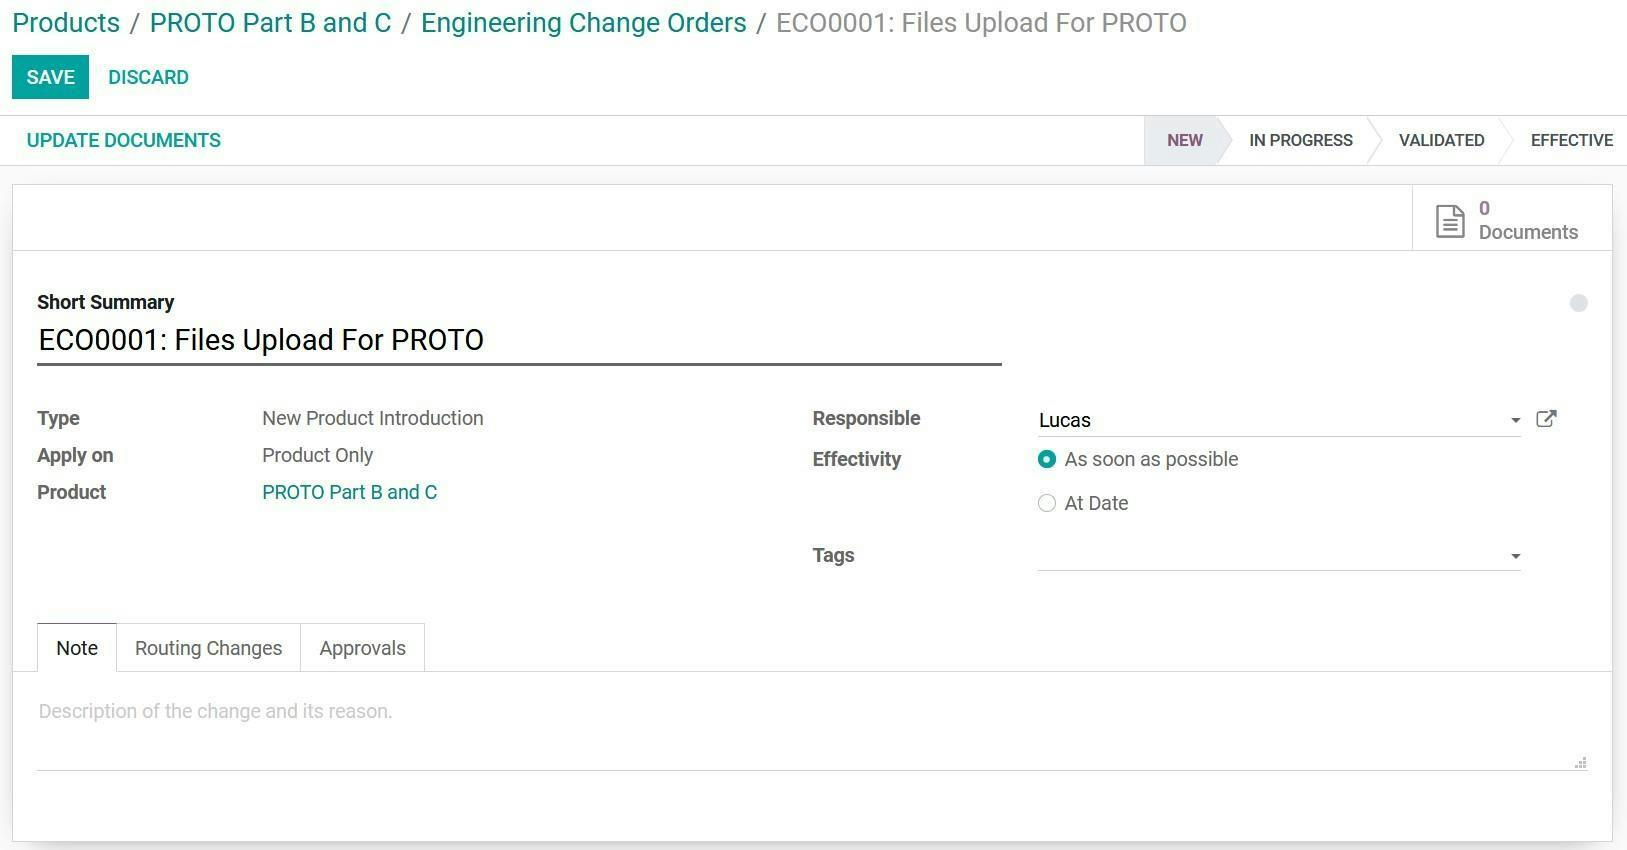
\includegraphics[width=439.35pt,height=229.49pt]{latexImage_48d0857ef2c5db6368cfa02666ce7133.png}}
\put(199.01,-74.38){\fontsize{12}{1}\usefont{T1}{ptm}{b}{n}\selectfont\color{color_29791}圖}
\put(211.01,-74.38){\fontsize{12}{1}\usefont{T1}{ptm}{b}{n}\selectfont\color{color_29791} }
\put(214.01,-74.38){\fontsize{12}{1}\usefont{T1}{ptm}{b}{n}\selectfont\color{color_29791}42}
\put(226.01,-74.38){\fontsize{12}{1}\usefont{T1}{ptm}{b}{n}\selectfont\color{color_29791} }
\put(228.89,-74.38){\fontsize{12}{1}\usefont{T1}{ptm}{b}{n}\selectfont\color{color_29791}為原型設計創建的}
\put(324.91,-74.38){\fontsize{12}{1}\usefont{T1}{ptm}{b}{n}\selectfont\color{color_29791} }
\put(327.91,-74.38){\fontsize{12}{1}\usefont{T1}{ptm}{b}{n}\selectfont\color{color_29791}B}
\put(335.938,-74.38){\fontsize{12}{1}\usefont{T1}{ptm}{b}{n}\selectfont\color{color_29791}OM}
\put(356.59,-74.38){\fontsize{12}{1}\usefont{T1}{ptm}{b}{n}\selectfont\color{color_29791} }
\put(359.47,-74.38){\fontsize{12}{1}\usefont{T1}{ptm}{b}{n}\selectfont\color{color_29791}概述}
\put(382.99,-74.38){\fontsize{12}{1}\usefont{T1}{ptm}{b}{n}\selectfont\color{color_29791} }
\put(82.944,-104.86){\fontsize{12}{1}\usefont{T1}{ptm}{m}{n}\selectfont\color{color_29791}說到這種缺乏上傳機會,我們可以注意到,在製作產品專案時,無法直接將有關}
\put(69.384,-122.74){\fontsize{12}{1}\usefont{T1}{ptm}{m}{n}\selectfont\color{color_29791}產品的檔上傳到專}
\put(165.38,-122.74){\fontsize{12}{1}\usefont{T1}{ptm}{m}{n}\selectfont\color{color_29791}案}
\put(177.38,-122.74){\fontsize{12}{1}\usefont{T1}{ptm}{m}{n}\selectfont\color{color_29791}。在我們的案例中,我們有關於我們正在原型製作的零件的}
\put(489.46,-122.74){\fontsize{12}{1}\usefont{T1}{ptm}{m}{n}\selectfont\color{color_29791} }
\put(69.384,-140.74){\fontsize{12}{1}\usefont{T1}{ptm}{m}{n}\selectfont\color{color_29791}C}
\put(77.424,-140.74){\fontsize{12}{1}\usefont{T1}{ptm}{m}{n}\selectfont\color{color_29791}A}
\put(86.06,-140.74){\fontsize{12}{1}\usefont{T1}{ptm}{m}{n}\selectfont\color{color_29791}D}
\put(94.7,-140.74){\fontsize{12}{1}\usefont{T1}{ptm}{m}{n}\selectfont\color{color_29791} }
\put(273.29,-140.74){\fontsize{12}{1}\usefont{T1}{ptm}{m}{n}\selectfont\color{color_29791}檔,從}
\put(309.31,-140.74){\fontsize{12}{1}\usefont{T1}{ptm}{m}{n}\selectfont\color{color_29791} }
\put(487.9,-140.74){\fontsize{12}{1}\usefont{T1}{ptm}{m}{n}\selectfont\color{color_29791}P}
\put(494.5,-140.74){\fontsize{12}{1}\usefont{T1}{ptm}{m}{n}\selectfont\color{color_29791}L}
\put(501.22,-140.74){\fontsize{12}{1}\usefont{T1}{ptm}{m}{n}\selectfont\color{color_29791}M}
\put(69.384,-158.62){\fontsize{12}{1}\usefont{T1}{ptm}{m}{n}\selectfont\color{color_29791}的角度來}
\put(117.38,-158.62){\fontsize{12}{1}\usefont{T1}{ptm}{m}{n}\selectfont\color{color_29791}看}
\put(129.38,-158.62){\fontsize{12}{1}\usefont{T1}{ptm}{m}{n}\selectfont\color{color_29791},無法以任何方式上傳這些檔將是一個完全失敗的過}
\put(405.43,-158.62){\fontsize{12}{1}\usefont{T1}{ptm}{m}{n}\selectfont\color{color_29791}程}
\put(417.43,-158.62){\fontsize{12}{1}\usefont{T1}{ptm}{m}{n}\selectfont\color{color_29791}。值得慶幸的是}
\put(501.46,-158.62){\fontsize{12}{1}\usefont{T1}{ptm}{m}{n}\selectfont\color{color_29791} }
\put(69.384,-176.5){\fontsize{12}{1}\usefont{T1}{ptm}{m}{n}\selectfont\color{color_29791},有一個解決方}
\put(153.38,-176.5){\fontsize{12}{1}\usefont{T1}{ptm}{m}{n}\selectfont\color{color_29791}法}
\put(165.38,-176.5){\fontsize{12}{1}\usefont{T1}{ptm}{m}{n}\selectfont\color{color_29791}。如第}
\put(201.41,-176.5){\fontsize{12}{1}\usefont{T1}{ptm}{m}{n}\selectfont\color{color_29791} }
\put(304.49,-176.5){\fontsize{12}{1}\usefont{T1}{ptm}{m}{n}\selectfont\color{color_29791}5.1.3.5}
\put(337.51,-176.5){\fontsize{12}{1}\usefont{T1}{ptm}{m}{n}\selectfont\color{color_29791} }
\put(440.62,-176.5){\fontsize{12}{1}\usefont{T1}{ptm}{m}{n}\selectfont\color{color_29791}節所述}
\put(476.62,-176.5){\fontsize{12}{1}\usefont{T1}{ptm}{m}{n}\selectfont\color{color_29791},}
\put(488.38,-176.5){\fontsize{12}{1}\usefont{T1}{ptm}{m}{n}\selectfont\color{color_29791}E}
\put(495.46,-176.5){\fontsize{12}{1}\usefont{T1}{ptm}{m}{n}\selectfont\color{color_29791}C}
\put(503.26,-176.5){\fontsize{12}{1}\usefont{T1}{ptm}{m}{n}\selectfont\color{color_29791}O}
\put(69.384,-194.14){\fontsize{12}{1}\usefont{T1}{ptm}{m}{n}\selectfont\color{color_29791}是鏈接到產品物料或物料清單並允許將上傳的檔附加到其中的物料。這是一個次要}
\put(69.384,-211.9){\fontsize{12}{1}\usefont{T1}{ptm}{m}{n}\selectfont\color{color_29791}的解決方}
\put(117.38,-211.9){\fontsize{12}{1}\usefont{T1}{ptm}{m}{n}\selectfont\color{color_29791}法}
\put(129.38,-211.9){\fontsize{12}{1}\usefont{T1}{ptm}{m}{n}\selectfont\color{color_29791},但基本上意味著如果我們想以任何有意義的方式將}
\put(405.43,-211.9){\fontsize{12}{1}\usefont{T1}{ptm}{m}{n}\selectfont\color{color_29791} }
\put(440.62,-211.9){\fontsize{12}{1}\usefont{T1}{ptm}{m}{n}\selectfont\color{color_29791} }
\put(487.3,-211.9){\fontsize{12}{1}\usefont{T1}{ptm}{m}{n}\selectfont\color{color_29791}C}
\put(495.1,-211.9){\fontsize{12}{1}\usefont{T1}{ptm}{m}{n}\selectfont\color{color_29791}AD}
\put(69.384,-229.54){\fontsize{12}{1}\usefont{T1}{ptm}{m}{n}\selectfont\color{color_29791}檔上傳到專}
\put(129.38,-229.54){\fontsize{12}{1}\usefont{T1}{ptm}{m}{n}\selectfont\color{color_29791}案}
\put(141.38,-229.54){\fontsize{12}{1}\usefont{T1}{ptm}{m}{n}\selectfont\color{color_29791},即使沒有進行}
\put(225.41,-229.54){\fontsize{12}{1}\usefont{T1}{ptm}{m}{n}\selectfont\color{color_29791}“}
\put(230.69,-229.54){\fontsize{12}{1}\usefont{T1}{ptm}{m}{n}\selectfont\color{color_29791} }
\put(233.69,-229.54){\fontsize{12}{1}\usefont{T1}{ptm}{m}{n}\selectfont\color{color_29791}更改}
\put(257.69,-229.54){\fontsize{12}{1}\usefont{T1}{ptm}{m}{n}\selectfont\color{color_29791}”}
\put(262.97,-229.54){\fontsize{12}{1}\usefont{T1}{ptm}{m}{n}\selectfont\color{color_29791} }
\put(63.024,-240.94){\fontsize{6}{1}\usefont{T1}{ptm}{m}{n}\selectfont\color{color_29791} }
\put(249.77,-494.31){\fontsize{12}{1}\usefont{T1}{ptm}{b}{n}\selectfont\color{color_29791}圖}
\put(261.77,-494.31){\fontsize{12}{1}\usefont{T1}{ptm}{b}{n}\selectfont\color{color_29791} }
\put(264.77,-494.31){\fontsize{12}{1}\usefont{T1}{ptm}{b}{n}\selectfont\color{color_29791}43 E}
\put(287.798,-494.31){\fontsize{12}{1}\usefont{T1}{ptm}{b}{n}\selectfont\color{color_29791}CO}
\put(305.81,-494.31){\fontsize{12}{1}\usefont{T1}{ptm}{b}{n}\selectfont\color{color_29791} }
\put(308.69,-494.31){\fontsize{12}{1}\usefont{T1}{ptm}{b}{n}\selectfont\color{color_29791}示例}
\put(332.23,-494.31){\fontsize{12}{1}\usefont{T1}{ptm}{b}{n}\selectfont\color{color_29791} }
\put(82.944,-526.23){\fontsize{12}{1}\usefont{T1}{ptm}{m}{n}\selectfont\color{color_29791}只能假設這}
\put(143.052,-526.23){\fontsize{12}{1}\usefont{T1}{ptm}{m}{n}\selectfont\color{color_29791}是}
\put(155.06,-526.23){\fontsize{12}{1}\usefont{T1}{ptm}{m}{n}\selectfont\color{color_29791}O}
\put(163.58,-526.23){\fontsize{12}{1}\usefont{T1}{ptm}{m}{n}\selectfont\color{color_29791}d}
\put(169.46,-526.23){\fontsize{12}{1}\usefont{T1}{ptm}{m}{n}\selectfont\color{color_29791}oo}
\put(181.49,-526.23){\fontsize{12}{1}\usefont{T1}{ptm}{m}{n}\selectfont\color{color_29791}團隊}
\put(205.598,-526.23){\fontsize{12}{1}\usefont{T1}{ptm}{m}{n}\selectfont\color{color_29791}戰略的一部}
\put(265.706,-526.23){\fontsize{12}{1}\usefont{T1}{ptm}{m}{n}\selectfont\color{color_29791}分,即在}
\put(313.814,-526.23){\fontsize{12}{1}\usefont{T1}{ptm}{m}{n}\selectfont\color{color_29791}其}
\put(325.99,-526.23){\fontsize{12}{1}\usefont{T1}{ptm}{m}{n}\selectfont\color{color_29791}E}
\put(333.19,-526.23){\fontsize{12}{1}\usefont{T1}{ptm}{m}{n}\selectfont\color{color_29791}R}
\put(341.11,-526.23){\fontsize{12}{1}\usefont{T1}{ptm}{m}{n}\selectfont\color{color_29791}P}
\put(347.83,-526.23){\fontsize{12}{1}\usefont{T1}{ptm}{m}{n}\selectfont\color{color_29791}基礎中將}
\put(395.83,-526.23){\fontsize{12}{1}\usefont{T1}{ptm}{m}{n}\selectfont\color{color_29791}P}
\put(402.43,-526.23){\fontsize{12}{1}\usefont{T1}{ptm}{m}{n}\selectfont\color{color_29791}L}
\put(409.63,-526.23){\fontsize{12}{1}\usefont{T1}{ptm}{m}{n}\selectfont\color{color_29791}M}
\put(420.43,-526.23){\fontsize{12}{1}\usefont{T1}{ptm}{m}{n}\selectfont\color{color_29791}作為}
\put(444.538,-526.23){\fontsize{12}{1}\usefont{T1}{ptm}{m}{n}\selectfont\color{color_29791}外部應用程}
\put(69.384,-544.11){\fontsize{12}{1}\usefont{T1}{ptm}{m}{n}\selectfont\color{color_29791}序}
\put(81.492,-544.11){\fontsize{12}{1}\usefont{T1}{ptm}{m}{n}\selectfont\color{color_29791}實}
\put(93.60001,-544.11){\fontsize{12}{1}\usefont{T1}{ptm}{m}{n}\selectfont\color{color_29791}施}
\put(105.708,-544.11){\fontsize{12}{1}\usefont{T1}{ptm}{m}{n}\selectfont\color{color_29791}。}
\put(117.816,-544.11){\fontsize{12}{1}\usefont{T1}{ptm}{m}{n}\selectfont\color{color_29791}這}
\put(129.924,-544.11){\fontsize{12}{1}\usefont{T1}{ptm}{m}{n}\selectfont\color{color_29791}是合}
\put(154.032,-544.11){\fontsize{12}{1}\usefont{T1}{ptm}{m}{n}\selectfont\color{color_29791}理}
\put(166.14,-544.11){\fontsize{12}{1}\usefont{T1}{ptm}{m}{n}\selectfont\color{color_29791}的}
\put(178.248,-544.11){\fontsize{12}{1}\usefont{T1}{ptm}{m}{n}\selectfont\color{color_29791},但}
\put(202.356,-544.11){\fontsize{12}{1}\usefont{T1}{ptm}{m}{n}\selectfont\color{color_29791}這}
\put(214.464,-544.11){\fontsize{12}{1}\usefont{T1}{ptm}{m}{n}\selectfont\color{color_29791}仍}
\put(226.572,-544.11){\fontsize{12}{1}\usefont{T1}{ptm}{m}{n}\selectfont\color{color_29791}然}
\put(238.68,-544.11){\fontsize{12}{1}\usefont{T1}{ptm}{m}{n}\selectfont\color{color_29791}是}
\put(250.788,-544.11){\fontsize{12}{1}\usefont{T1}{ptm}{m}{n}\selectfont\color{color_29791}該軟}
\put(274.896,-544.11){\fontsize{12}{1}\usefont{T1}{ptm}{m}{n}\selectfont\color{color_29791}體}
\put(287.004,-544.11){\fontsize{12}{1}\usefont{T1}{ptm}{m}{n}\selectfont\color{color_29791}介}
\put(299.112,-544.11){\fontsize{12}{1}\usefont{T1}{ptm}{m}{n}\selectfont\color{color_29791}面為}
\put(323.22,-544.11){\fontsize{12}{1}\usefont{T1}{ptm}{m}{n}\selectfont\color{color_29791}數}
\put(335.328,-544.11){\fontsize{12}{1}\usefont{T1}{ptm}{m}{n}\selectfont\color{color_29791}不}
\put(347.436,-544.11){\fontsize{12}{1}\usefont{T1}{ptm}{m}{n}\selectfont\color{color_29791}多}
\put(359.544,-544.11){\fontsize{12}{1}\usefont{T1}{ptm}{m}{n}\selectfont\color{color_29791}的}
\put(371.652,-544.11){\fontsize{12}{1}\usefont{T1}{ptm}{m}{n}\selectfont\color{color_29791}不那}
\put(395.76,-544.11){\fontsize{12}{1}\usefont{T1}{ptm}{m}{n}\selectfont\color{color_29791}麼}
\put(407.868,-544.11){\fontsize{12}{1}\usefont{T1}{ptm}{m}{n}\selectfont\color{color_29791}簡}
\put(419.976,-544.11){\fontsize{12}{1}\usefont{T1}{ptm}{m}{n}\selectfont\color{color_29791}單的}
\put(444.084,-544.11){\fontsize{12}{1}\usefont{T1}{ptm}{m}{n}\selectfont\color{color_29791}方}
\put(456.192,-544.11){\fontsize{12}{1}\usefont{T1}{ptm}{m}{n}\selectfont\color{color_29791}面}
\put(468.3,-544.11){\fontsize{12}{1}\usefont{T1}{ptm}{m}{n}\selectfont\color{color_29791}之}
\put(480.4081,-544.11){\fontsize{12}{1}\usefont{T1}{ptm}{m}{n}\selectfont\color{color_29791}一。}
\put(69.384,-561.99){\fontsize{12}{1}\usefont{T1}{ptm}{m}{n}\selectfont\color{color_29791}這是一個非常有價}
\put(166.224,-561.99){\fontsize{12}{1}\usefont{T1}{ptm}{m}{n}\selectfont\color{color_29791}值的}
\put(190.344,-561.99){\fontsize{12}{1}\usefont{T1}{ptm}{m}{n}\selectfont\color{color_29791}功能,但它有些隱}
\put(287.184,-561.99){\fontsize{12}{1}\usefont{T1}{ptm}{m}{n}\selectfont\color{color_29791}藏。}
\put(311.304,-561.99){\fontsize{12}{1}\usefont{T1}{ptm}{m}{n}\selectfont\color{color_29791}文件圖示僅在創建}
\put(408.144,-561.99){\fontsize{12}{1}\usefont{T1}{ptm}{m}{n}\selectfont\color{color_29791}並保}
\put(432.264,-561.99){\fontsize{12}{1}\usefont{T1}{ptm}{m}{n}\selectfont\color{color_29791}存}
\put(444.46,-561.99){\fontsize{12}{1}\usefont{T1}{ptm}{m}{n}\selectfont\color{color_29791}E}
\put(451.66,-561.99){\fontsize{12}{1}\usefont{T1}{ptm}{m}{n}\selectfont\color{color_29791}C}
\put(459.58,-561.99){\fontsize{12}{1}\usefont{T1}{ptm}{m}{n}\selectfont\color{color_29791}O}
\put(468.34,-561.99){\fontsize{12}{1}\usefont{T1}{ptm}{m}{n}\selectfont\color{color_29791}後才會}
\put(69.384,-580.02){\fontsize{12}{1}\usefont{T1}{ptm}{m}{n}\selectfont\color{color_29791}出現在右上角(}
\put(153.38,-580.02){\fontsize{12}{1}\usefont{T1}{ptm}{m}{n}\selectfont\color{color_29791}圖}
\put(164.3,-580.02){\fontsize{12}{1}\usefont{T1}{ptm}{m}{n}\selectfont\color{color_29791} }
\put(169.22,-580.02){\fontsize{12}{1}\usefont{T1}{ptm}{m}{n}\selectfont\color{color_29791}43}
\put(181.37,-580.02){\fontsize{12}{1}\usefont{T1}{ptm}{m}{n}\selectfont\color{color_29791})。}
\put(205.37,-580.02){\fontsize{12}{1}\usefont{T1}{ptm}{m}{n}\selectfont\color{color_29791} }
\end{picture}
\newpage
\begin{tikzpicture}[overlay]\path(0pt,0pt);\end{tikzpicture}
\begin{picture}(-5,0)(2.5,0)
\put(500.26,-727.616){\fontsize{12}{1}\usefont{T1}{ptm}{m}{n}\selectfont\color{color_29791}47}
\put(511.78,-727.616){\fontsize{12}{1}\usefont{T1}{ptm}{m}{n}\selectfont\color{color_29791} }
\put(63.024,-726.896){\fontsize{9.96}{1}\usefont{T1}{ptm}{m}{n}\selectfont\color{color_29791} }
\put(73.75,-674.7){\includegraphics[width=441.77pt,height=198.7pt]{latexImage_3a7261bd45455390c480a5d603c8a4d0.png}}
\put(510.22,-250.21){\fontsize{9.96}{1}\usefont{T1}{ptm}{m}{n}\selectfont\color{color_29791} }
\put(240.89,-265.45){\fontsize{12}{1}\usefont{T1}{ptm}{b}{n}\selectfont\color{color_29791}圖}
\put(252.89,-265.45){\fontsize{12}{1}\usefont{T1}{ptm}{b}{n}\selectfont\color{color_29791}44}
\put(264.89,-265.45){\fontsize{12}{1}\usefont{T1}{ptm}{b}{n}\selectfont\color{color_29791} }
\put(267.89,-265.45){\fontsize{12}{1}\usefont{T1}{ptm}{b}{n}\selectfont\color{color_29791}E}
\put(275.918,-265.45){\fontsize{12}{1}\usefont{T1}{ptm}{b}{n}\selectfont\color{color_29791}CO}
\put(293.93,-265.45){\fontsize{12}{1}\usefont{T1}{ptm}{b}{n}\selectfont\color{color_29791}附}
\put(305.81,-265.45){\fontsize{12}{1}\usefont{T1}{ptm}{b}{n}\selectfont\color{color_29791}件}
\put(317.69,-265.45){\fontsize{12}{1}\usefont{T1}{ptm}{b}{n}\selectfont\color{color_29791}概}
\put(329.45,-265.45){\fontsize{12}{1}\usefont{T1}{ptm}{b}{n}\selectfont\color{color_29791}覽}
\put(341.23,-265.45){\fontsize{12}{1}\usefont{T1}{ptm}{b}{n}\selectfont\color{color_29791} }
\put(82.944,-297.01){\fontsize{12}{1}\usefont{T1}{ptm}{m}{n}\selectfont\color{color_29791}由}
\put(94.94,-297.01){\fontsize{12}{1}\usefont{T1}{ptm}{m}{n}\selectfont\color{color_29791}於}
\put(106.94,-297.01){\fontsize{12}{1}\usefont{T1}{ptm}{m}{n}\selectfont\color{color_29791}Odo}
\put(127.58,-297.01){\fontsize{12}{1}\usefont{T1}{ptm}{m}{n}\selectfont\color{color_29791}o}
\put(133.58,-297.01){\fontsize{12}{1}\usefont{T1}{ptm}{m}{n}\selectfont\color{color_29791}和}
\put(145.58,-297.01){\fontsize{12}{1}\usefont{T1}{ptm}{m}{n}\selectfont\color{color_29791}C}
\put(153.62,-297.01){\fontsize{12}{1}\usefont{T1}{ptm}{m}{n}\selectfont\color{color_29791}AD}
\put(170.9,-297.01){\fontsize{12}{1}\usefont{T1}{ptm}{m}{n}\selectfont\color{color_29791}軟體}
\put(194.78,-297.01){\fontsize{12}{1}\usefont{T1}{ptm}{m}{n}\selectfont\color{color_29791}之間沒有直接集成,因此上傳檔不會導致產品元數據自動更}
\put(69.384,-314.89){\fontsize{12}{1}\usefont{T1}{ptm}{m}{n}\selectfont\color{color_29791}改}
\put(81.384,-314.89){\fontsize{12}{1}\usefont{T1}{ptm}{m}{n}\selectfont\color{color_29791}。}
\put(93.38,-314.89){\fontsize{12}{1}\usefont{T1}{ptm}{m}{n}\selectfont\color{color_29791}從}
\put(105.38,-314.89){\fontsize{12}{1}\usefont{T1}{ptm}{m}{n}\selectfont\color{color_29791}P}
\put(112.22,-314.89){\fontsize{12}{1}\usefont{T1}{ptm}{m}{n}\selectfont\color{color_29791}L}
\put(119.3,-314.89){\fontsize{12}{1}\usefont{T1}{ptm}{m}{n}\selectfont\color{color_29791}M}
\put(129.98,-314.89){\fontsize{12}{1}\usefont{T1}{ptm}{m}{n}\selectfont\color{color_29791}的角度來}
\put(177.98,-314.89){\fontsize{12}{1}\usefont{T1}{ptm}{m}{n}\selectfont\color{color_29791}看}
\put(190.13,-314.89){\fontsize{12}{1}\usefont{T1}{ptm}{m}{n}\selectfont\color{color_29791},這並不理想,但它仍然是一個實現良好的功能。通過允許}
\put(69.384,-332.77){\fontsize{12}{1}\usefont{T1}{ptm}{m}{n}\selectfont\color{color_29791}產品項目不僅直接連結到一個現有的}
\put(261.41,-332.77){\fontsize{12}{1}\usefont{T1}{ptm}{m}{n}\selectfont\color{color_29791} }
\put(284.57,-332.77){\fontsize{12}{1}\usefont{T1}{ptm}{m}{n}\selectfont\color{color_29791}EC}
\put(299.93,-332.77){\fontsize{12}{1}\usefont{T1}{ptm}{m}{n}\selectfont\color{color_29791}O}
\put(308.57,-332.77){\fontsize{12}{1}\usefont{T1}{ptm}{m}{n}\selectfont\color{color_29791},而且連結到曾經}
\put(404.45,-332.77){\fontsize{12}{1}\usefont{T1}{ptm}{m}{n}\selectfont\color{color_29791}應用於該專案的所}
\put(500.5,-332.77){\fontsize{12}{1}\usefont{T1}{ptm}{m}{n}\selectfont\color{color_29791}有}
\put(511.78,-332.77){\fontsize{12}{1}\usefont{T1}{ptm}{m}{n}\selectfont\color{color_29791} }
\put(69.384,-350.77){\fontsize{12}{1}\usefont{T1}{ptm}{m}{n}\selectfont\color{color_29791}EC}
\put(84.744,-350.77){\fontsize{12}{1}\usefont{T1}{ptm}{m}{n}\selectfont\color{color_29791}O }
\put(96.38,-350.77){\fontsize{12}{1}\usefont{T1}{ptm}{m}{n}\selectfont\color{color_29791}的清單,該軟體}
\put(180.26,-350.77){\fontsize{12}{1}\usefont{T1}{ptm}{m}{n}\selectfont\color{color_29791}在跟蹤版本控制和開發方面做得很}
\put(360.31,-350.77){\fontsize{12}{1}\usefont{T1}{ptm}{m}{n}\selectfont\color{color_29791}好}
\put(372.31,-350.77){\fontsize{12}{1}\usefont{T1}{ptm}{m}{n}\selectfont\color{color_29791}。}
\put(384.31,-350.77){\fontsize{12}{1}\usefont{T1}{ptm}{m}{n}\selectfont\color{color_29791} }
\put(82.944,-383.41){\fontsize{12}{1}\usefont{T1}{ptm}{m}{n}\selectfont\color{color_29791}為了過程式控制,可以做一些有趣的事情,即在操作中添加品質控制點。這允許}
\put(69.384,-401.29){\fontsize{12}{1}\usefont{T1}{ptm}{m}{n}\selectfont\color{color_29791}負}
\put(81.492,-401.29){\fontsize{12}{1}\usefont{T1}{ptm}{m}{n}\selectfont\color{color_29791}責}
\put(93.60001,-401.29){\fontsize{12}{1}\usefont{T1}{ptm}{m}{n}\selectfont\color{color_29791}人}
\put(105.708,-401.29){\fontsize{12}{1}\usefont{T1}{ptm}{m}{n}\selectfont\color{color_29791}員}
\put(117.936,-401.29){\fontsize{12}{1}\usefont{T1}{ptm}{m}{n}\selectfont\color{color_29791}在}
\put(130.044,-401.29){\fontsize{12}{1}\usefont{T1}{ptm}{m}{n}\selectfont\color{color_29791}生}
\put(142.152,-401.29){\fontsize{12}{1}\usefont{T1}{ptm}{m}{n}\selectfont\color{color_29791}產}
\put(154.38,-401.29){\fontsize{12}{1}\usefont{T1}{ptm}{m}{n}\selectfont\color{color_29791}過}
\put(166.488,-401.29){\fontsize{12}{1}\usefont{T1}{ptm}{m}{n}\selectfont\color{color_29791}程}
\put(178.596,-401.29){\fontsize{12}{1}\usefont{T1}{ptm}{m}{n}\selectfont\color{color_29791}中}
\put(190.824,-401.29){\fontsize{12}{1}\usefont{T1}{ptm}{m}{n}\selectfont\color{color_29791}向}
\put(202.932,-401.29){\fontsize{12}{1}\usefont{T1}{ptm}{m}{n}\selectfont\color{color_29791}工}
\put(215.04,-401.29){\fontsize{12}{1}\usefont{T1}{ptm}{m}{n}\selectfont\color{color_29791}程}
\put(227.148,-401.29){\fontsize{12}{1}\usefont{T1}{ptm}{m}{n}\selectfont\color{color_29791}團}
\put(239.376,-401.29){\fontsize{12}{1}\usefont{T1}{ptm}{m}{n}\selectfont\color{color_29791}隊}
\put(251.484,-401.29){\fontsize{12}{1}\usefont{T1}{ptm}{m}{n}\selectfont\color{color_29791}提}
\put(263.592,-401.29){\fontsize{12}{1}\usefont{T1}{ptm}{m}{n}\selectfont\color{color_29791}供}
\put(275.82,-401.29){\fontsize{12}{1}\usefont{T1}{ptm}{m}{n}\selectfont\color{color_29791}有}
\put(287.928,-401.29){\fontsize{12}{1}\usefont{T1}{ptm}{m}{n}\selectfont\color{color_29791}關}
\put(300.036,-401.29){\fontsize{12}{1}\usefont{T1}{ptm}{m}{n}\selectfont\color{color_29791}要}
\put(312.264,-401.29){\fontsize{12}{1}\usefont{T1}{ptm}{m}{n}\selectfont\color{color_29791}點}
\put(324.372,-401.29){\fontsize{12}{1}\usefont{T1}{ptm}{m}{n}\selectfont\color{color_29791}的}
\put(336.48,-401.29){\fontsize{12}{1}\usefont{T1}{ptm}{m}{n}\selectfont\color{color_29791}反}
\put(348.588,-401.29){\fontsize{12}{1}\usefont{T1}{ptm}{m}{n}\selectfont\color{color_29791}饋}
\put(360.816,-401.29){\fontsize{12}{1}\usefont{T1}{ptm}{m}{n}\selectfont\color{color_29791}。}
\put(372.924,-401.29){\fontsize{12}{1}\usefont{T1}{ptm}{m}{n}\selectfont\color{color_29791}在}
\put(385.032,-401.29){\fontsize{12}{1}\usefont{T1}{ptm}{m}{n}\selectfont\color{color_29791}我}
\put(397.26,-401.29){\fontsize{12}{1}\usefont{T1}{ptm}{m}{n}\selectfont\color{color_29791}們}
\put(409.368,-401.29){\fontsize{12}{1}\usefont{T1}{ptm}{m}{n}\selectfont\color{color_29791}的}
\put(421.476,-401.29){\fontsize{12}{1}\usefont{T1}{ptm}{m}{n}\selectfont\color{color_29791}案}
\put(433.704,-401.29){\fontsize{12}{1}\usefont{T1}{ptm}{m}{n}\selectfont\color{color_29791}例}
\put(445.812,-401.29){\fontsize{12}{1}\usefont{T1}{ptm}{m}{n}\selectfont\color{color_29791}中}
\put(457.92,-401.29){\fontsize{12}{1}\usefont{T1}{ptm}{m}{n}\selectfont\color{color_29791},}
\put(470.028,-401.29){\fontsize{12}{1}\usefont{T1}{ptm}{m}{n}\selectfont\color{color_29791}我}
\put(482.256,-401.29){\fontsize{12}{1}\usefont{T1}{ptm}{m}{n}\selectfont\color{color_29791}們}
\put(494.364,-401.29){\fontsize{12}{1}\usefont{T1}{ptm}{m}{n}\selectfont\color{color_29791}擔}
\put(69.384,-419.19){\fontsize{12}{1}\usefont{T1}{ptm}{m}{n}\selectfont\color{color_29791}心}
\put(81.384,-419.19){\fontsize{12}{1}\usefont{T1}{ptm}{m}{n}\selectfont\color{color_29791}3D}
\put(95.9,-419.19){\fontsize{12}{1}\usefont{T1}{ptm}{m}{n}\selectfont\color{color_29791}列印翹曲。這是}
\put(180.008,-419.19){\fontsize{12}{1}\usefont{T1}{ptm}{m}{n}\selectfont\color{color_29791}在}
\put(192.17,-419.19){\fontsize{12}{1}\usefont{T1}{ptm}{m}{n}\selectfont\color{color_29791}3D}
\put(206.69,-419.19){\fontsize{12}{1}\usefont{T1}{ptm}{m}{n}\selectfont\color{color_29791}列印過程中溫度變}
\put(302.798,-419.19){\fontsize{12}{1}\usefont{T1}{ptm}{m}{n}\selectfont\color{color_29791}化}
\put(314.906,-419.19){\fontsize{12}{1}\usefont{T1}{ptm}{m}{n}\selectfont\color{color_29791}很大時發生的情況。為}
\put(435.014,-419.19){\fontsize{12}{1}\usefont{T1}{ptm}{m}{n}\selectfont\color{color_29791}此,將創建一}
\put(69.384,-437.07){\fontsize{12}{1}\usefont{T1}{ptm}{m}{n}\selectfont\color{color_29791}個品質控制點專案}
\put(164.532,-437.07){\fontsize{12}{1}\usefont{T1}{ptm}{m}{n}\selectfont\color{color_29791}(圖}
\put(188.45,-437.07){\fontsize{12}{1}\usefont{T1}{ptm}{m}{n}\selectfont\color{color_29791} }
\put(69.384,-455.07){\fontsize{11.04}{1}\usefont{T1}{ptm}{m}{n}\selectfont\color{color_29791}45}
\put(80.424,-455.07){\fontsize{11.04}{1}\usefont{T1}{ptm}{m}{n}\selectfont\color{color_29791})}
\put(91.34,-455.07){\fontsize{11.04}{1}\usefont{T1}{uarial}{m}{n}\selectfont\color{color_29791} }
\put(93.38,-455.07){\fontsize{12}{1}\usefont{T1}{ptm}{m}{n}\selectfont\color{color_29791},該專}
\put(129.26,-455.07){\fontsize{12}{1}\usefont{T1}{ptm}{m}{n}\selectfont\color{color_29791}案將詢}
\put(165.14,-455.07){\fontsize{12}{1}\usefont{T1}{ptm}{m}{n}\selectfont\color{color_29791}問操}
\put(189.02,-455.07){\fontsize{12}{1}\usefont{T1}{ptm}{m}{n}\selectfont\color{color_29791}作員}
\put(212.9,-455.07){\fontsize{12}{1}\usefont{T1}{ptm}{m}{n}\selectfont\color{color_29791}以檢查}
\put(248.78,-455.07){\fontsize{12}{1}\usefont{T1}{ptm}{m}{n}\selectfont\color{color_29791}工件中}
\put(284.66,-455.07){\fontsize{12}{1}\usefont{T1}{ptm}{m}{n}\selectfont\color{color_29791}是否}
\put(308.54,-455.07){\fontsize{12}{1}\usefont{T1}{ptm}{m}{n}\selectfont\color{color_29791}存在}
\put(332.42,-455.07){\fontsize{12}{1}\usefont{T1}{ptm}{m}{n}\selectfont\color{color_29791}翹曲並}
\put(368.3,-455.07){\fontsize{12}{1}\usefont{T1}{ptm}{m}{n}\selectfont\color{color_29791}標記通}
\put(404.18,-455.07){\fontsize{12}{1}\usefont{T1}{ptm}{m}{n}\selectfont\color{color_29791}過或}
\put(428.06,-455.07){\fontsize{12}{1}\usefont{T1}{ptm}{m}{n}\selectfont\color{color_29791}失敗}
\put(451.94,-455.07){\fontsize{12}{1}\usefont{T1}{ptm}{m}{n}\selectfont\color{color_29791}。}
\put(464.02,-455.07){\fontsize{12}{1}\usefont{T1}{ptm}{m}{n}\selectfont\color{color_29791} }
\put(63.024,-472.11){\fontsize{9.96}{1}\usefont{T1}{ptm}{m}{n}\selectfont\color{color_29791} }
\put(207.41,-694.856){\fontsize{12}{1}\usefont{T1}{ptm}{b}{n}\selectfont\color{color_29791}圖}
\put(219.41,-694.856){\fontsize{12}{1}\usefont{T1}{ptm}{b}{n}\selectfont\color{color_29791}45}
\put(231.41,-694.856){\fontsize{12}{1}\usefont{T1}{ptm}{b}{n}\selectfont\color{color_29791}原型生}
\put(267.29,-694.856){\fontsize{12}{1}\usefont{T1}{ptm}{b}{n}\selectfont\color{color_29791}產的品}
\put(303.17,-694.856){\fontsize{12}{1}\usefont{T1}{ptm}{b}{n}\selectfont\color{color_29791}質控}
\put(327.05,-694.856){\fontsize{12}{1}\usefont{T1}{ptm}{b}{n}\selectfont\color{color_29791}制點專}
\put(362.93,-694.856){\fontsize{12}{1}\usefont{T1}{ptm}{b}{n}\selectfont\color{color_29791}案}
\put(374.83,-694.856){\fontsize{12}{1}\usefont{T1}{ptm}{b}{n}\selectfont\color{color_29791} }
\put(73.75,-250.1){\includegraphics[width=436.35pt,height=189.1pt]{latexImage_403ad3b9ccc9a753a743c835109563b9.png}}
\end{picture}
\newpage
\begin{tikzpicture}[overlay]\path(0pt,0pt);\end{tikzpicture}
\begin{picture}(-5,0)(2.5,0)
\put(500.26,-727.616){\fontsize{12}{1}\usefont{T1}{ptm}{m}{n}\selectfont\color{color_29791}48}
\put(511.78,-727.616){\fontsize{12}{1}\usefont{T1}{ptm}{m}{n}\selectfont\color{color_29791} }
\put(63.024,-726.896){\fontsize{9.96}{1}\usefont{T1}{ptm}{m}{n}\selectfont\color{color_29791} }
\put(70.05,-523.65){\includegraphics[width=440.35pt,height=328.05pt]{latexImage_0405f8562b8d3b68ccdac4bc62ba5caa.png}}
\put(69.384,-102.94){\fontsize{12}{1}\usefont{T1}{ptm}{m}{n}\selectfont\color{color_29791}原型周期的最後一步是生產用於測試和評估的原型。在}
\put(357.43,-102.94){\fontsize{12}{1}\usefont{T1}{ptm}{m}{n}\selectfont\color{color_29791}Odo}
\put(378.07,-102.94){\fontsize{12}{1}\usefont{T1}{ptm}{m}{n}\selectfont\color{color_29791}o}
\put(384.07,-102.94){\fontsize{12}{1}\usefont{T1}{ptm}{m}{n}\selectfont\color{color_29791}中,製作是一件非常簡}
\put(69.384,-120.82){\fontsize{12}{1}\usefont{T1}{ptm}{m}{n}\selectfont\color{color_29791}單的事}
\put(105.38,-120.82){\fontsize{12}{1}\usefont{T1}{ptm}{m}{n}\selectfont\color{color_29791}情}
\put(117.38,-120.82){\fontsize{12}{1}\usefont{T1}{ptm}{m}{n}\selectfont\color{color_29791},也是我們之前所做的一切都彙集在一起的}
\put(345.43,-120.82){\fontsize{12}{1}\usefont{T1}{ptm}{m}{n}\selectfont\color{color_29791}點}
\put(357.43,-120.82){\fontsize{12}{1}\usefont{T1}{ptm}{m}{n}\selectfont\color{color_29791}。元數據和已創建的物料允}
\put(69.384,-138.7){\fontsize{12}{1}\usefont{T1}{ptm}{m}{n}\selectfont\color{color_29791}許我們啟動製造訂單}
\put(177.38,-138.7){\fontsize{12}{1}\usefont{T1}{ptm}{m}{n}\selectfont\color{color_29791} }
\put(445.3,-138.7){\fontsize{12}{1}\usefont{T1}{ptm}{m}{n}\selectfont\color{color_29791}(}
\put(457.3,-138.7){\fontsize{12}{1}\usefont{T1}{ptm}{m}{n}\selectfont\color{color_29791}M}
\put(467.98,-138.7){\fontsize{12}{1}\usefont{T1}{ptm}{m}{n}\selectfont\color{color_29791}O}
\put(476.62,-138.7){\fontsize{12}{1}\usefont{T1}{ptm}{m}{n}\selectfont\color{color_29791})(}
\put(500.62,-138.7){\fontsize{12}{1}\usefont{T1}{ptm}{m}{n}\selectfont\color{color_29791}圖}
\put(511.66,-138.7){\fontsize{12}{1}\usefont{T1}{ptm}{m}{n}\selectfont\color{color_29791} }
\put(69.384,-156.58){\fontsize{11.04}{1}\usefont{T1}{ptm}{m}{n}\selectfont\color{color_29791}46}
\put(80.424,-156.58){\fontsize{11.04}{1}\usefont{T1}{ptm}{m}{n}\selectfont\color{color_29791})}
\put(91.34,-156.58){\fontsize{11.04}{1}\usefont{T1}{uarial}{m}{n}\selectfont\color{color_29791} }
\put(93.38,-156.58){\fontsize{12}{1}\usefont{T1}{ptm}{m}{n}\selectfont\color{color_29791}。這反過來又從物}
\put(188.528,-156.58){\fontsize{12}{1}\usefont{T1}{ptm}{m}{n}\selectfont\color{color_29791}料清}
\put(212.396,-156.58){\fontsize{12}{1}\usefont{T1}{ptm}{m}{n}\selectfont\color{color_29791}單中列出的操作和}
\put(307.544,-156.58){\fontsize{12}{1}\usefont{T1}{ptm}{m}{n}\selectfont\color{color_29791}元件}
\put(331.412,-156.58){\fontsize{12}{1}\usefont{T1}{ptm}{m}{n}\selectfont\color{color_29791}中提取必要的工單}
\put(426.56,-156.58){\fontsize{12}{1}\usefont{T1}{ptm}{m}{n}\selectfont\color{color_29791}。為}
\put(450.428,-156.58){\fontsize{12}{1}\usefont{T1}{ptm}{m}{n}\selectfont\color{color_29791}製造操作}
\put(69.384,-174.7){\fontsize{12}{1}\usefont{T1}{ptm}{m}{n}\selectfont\color{color_29791}員顯示工單,並且}
\put(164.532,-174.7){\fontsize{12}{1}\usefont{T1}{ptm}{m}{n}\selectfont\color{color_29791}可以}
\put(188.4,-174.7){\fontsize{12}{1}\usefont{T1}{ptm}{m}{n}\selectfont\color{color_29791}開始}
\put(212.21,-174.7){\fontsize{12}{1}\usefont{T1}{ptm}{m}{n}\selectfont\color{color_29791}/}
\put(215.45,-174.7){\fontsize{12}{1}\usefont{T1}{ptm}{m}{n}\selectfont\color{color_29791}跟蹤生產。}
\put(274.97,-174.7){\fontsize{12}{1}\usefont{T1}{ptm}{m}{n}\selectfont\color{color_29791} }
\put(63.024,-191.74){\fontsize{9.96}{1}\usefont{T1}{ptm}{m}{n}\selectfont\color{color_29791} }
\put(240.41,-551.91){\fontsize{12}{1}\usefont{T1}{ptm}{b}{n}\selectfont\color{color_29791}圖}
\put(252.41,-551.91){\fontsize{12}{1}\usefont{T1}{ptm}{b}{n}\selectfont\color{color_29791} }
\put(255.41,-551.91){\fontsize{12}{1}\usefont{T1}{ptm}{b}{n}\selectfont\color{color_29791}46}
\put(267.41,-551.91){\fontsize{12}{1}\usefont{T1}{ptm}{b}{n}\selectfont\color{color_29791} }
\put(270.29,-551.91){\fontsize{12}{1}\usefont{T1}{ptm}{b}{n}\selectfont\color{color_29791}製}
\put(282.17,-551.91){\fontsize{12}{1}\usefont{T1}{ptm}{b}{n}\selectfont\color{color_29791}造訂}
\put(306.05,-551.91){\fontsize{12}{1}\usefont{T1}{ptm}{b}{n}\selectfont\color{color_29791}單}
\put(317.93,-551.91){\fontsize{12}{1}\usefont{T1}{ptm}{b}{n}\selectfont\color{color_29791}說}
\put(329.81,-551.91){\fontsize{12}{1}\usefont{T1}{ptm}{b}{n}\selectfont\color{color_29791}明}
\put(341.83,-551.91){\fontsize{12}{1}\usefont{T1}{ptm}{b}{n}\selectfont\color{color_29791} }
\put(82.944,-583.74){\fontsize{12}{1}\usefont{T1}{ptm}{m}{n}\selectfont\color{color_29791}在大多數情況}
\put(154.94,-583.74){\fontsize{12}{1}\usefont{T1}{ptm}{m}{n}\selectfont\color{color_29791}下}
\put(166.94,-583.74){\fontsize{12}{1}\usefont{T1}{ptm}{m}{n}\selectfont\color{color_29791},此操作非常自動化和清晰。然而,從}
\put(370.99,-583.74){\fontsize{12}{1}\usefont{T1}{ptm}{m}{n}\selectfont\color{color_29791}Odoo}
\put(397.63,-583.74){\fontsize{12}{1}\usefont{T1}{ptm}{m}{n}\selectfont\color{color_29791} }
\put(453.1,-583.74){\fontsize{12}{1}\usefont{T1}{ptm}{m}{n}\selectfont\color{color_29791}V13}
\put(473.74,-583.74){\fontsize{12}{1}\usefont{T1}{ptm}{m}{n}\selectfont\color{color_29791}到}
\put(485.74,-583.74){\fontsize{12}{1}\usefont{T1}{ptm}{m}{n}\selectfont\color{color_29791}O}
\put(494.14,-583.74){\fontsize{12}{1}\usefont{T1}{ptm}{m}{n}\selectfont\color{color_29791}d}
\put(499.9,-583.74){\fontsize{12}{1}\usefont{T1}{ptm}{m}{n}\selectfont\color{color_29791}o}
\put(505.78,-583.74){\fontsize{12}{1}\usefont{T1}{ptm}{m}{n}\selectfont\color{color_29791}o}
\put(511.54,-583.74){\fontsize{12}{1}\usefont{T1}{ptm}{m}{n}\selectfont\color{color_29791} }
\put(69.384,-601.62){\fontsize{12}{1}\usefont{T1}{ptm}{m}{n}\selectfont\color{color_29791}V1}
\put(84.024,-601.62){\fontsize{12}{1}\usefont{T1}{ptm}{m}{n}\selectfont\color{color_29791}4}
\put(90.02,-601.62){\fontsize{12}{1}\usefont{T1}{ptm}{m}{n}\selectfont\color{color_29791}的結構變化導致了一些問題。在很長一段時間里,該軟體命令使用一個名為}
\put(486.1,-601.62){\fontsize{12}{1}\usefont{T1}{ptm}{m}{n}\selectfont\color{color_29791}“}
\put(491.38,-601.62){\fontsize{12}{1}\usefont{T1}{ptm}{m}{n}\selectfont\color{color_29791}R}
\put(499.408,-601.62){\fontsize{12}{1}\usefont{T1}{ptm}{m}{n}\selectfont\color{color_29791}ou }
\put(69.384,-619.5){\fontsize{12}{1}\usefont{T1}{ptm}{m}{n}\selectfont\color{color_29791}t}
\put(72.744,-619.5){\fontsize{12}{1}\usefont{T1}{ptm}{m}{n}\selectfont\color{color_29791}e”}
\put(83.304,-619.5){\fontsize{12}{1}\usefont{T1}{ptm}{m}{n}\selectfont\color{color_29791}的額外專案類來執}
\put(179.3,-619.5){\fontsize{12}{1}\usefont{T1}{ptm}{m}{n}\selectfont\color{color_29791}行}
\put(191.45,-619.5){\fontsize{12}{1}\usefont{T1}{ptm}{m}{n}\selectfont\color{color_29791}操作。這些是產品在庫存和製造中移動的基本部}
\put(443.5,-619.5){\fontsize{12}{1}\usefont{T1}{ptm}{m}{n}\selectfont\color{color_29791}分}
\put(455.5,-619.5){\fontsize{12}{1}\usefont{T1}{ptm}{m}{n}\selectfont\color{color_29791},但由於}
\put(69.384,-637.38){\fontsize{12}{1}\usefont{T1}{ptm}{m}{n}\selectfont\color{color_29791}某種原}
\put(105.38,-637.38){\fontsize{12}{1}\usefont{T1}{ptm}{m}{n}\selectfont\color{color_29791}因}
\put(117.38,-637.38){\fontsize{12}{1}\usefont{T1}{ptm}{m}{n}\selectfont\color{color_29791},在新版本的製造方面被放棄了,取而代之的是內置在}
\put(405.43,-637.38){\fontsize{12}{1}\usefont{T1}{ptm}{m}{n}\selectfont\color{color_29791} }
\put(453.1,-637.38){\fontsize{12}{1}\usefont{T1}{ptm}{m}{n}\selectfont\color{color_29791} }
\put(485.38,-637.38){\fontsize{12}{1}\usefont{T1}{ptm}{m}{n}\selectfont\color{color_29791}B}
\put(493.06,-637.38){\fontsize{12}{1}\usefont{T1}{ptm}{m}{n}\selectfont\color{color_29791}OM}
\put(69.384,-655.26){\fontsize{12}{1}\usefont{T1}{ptm}{m}{n}\selectfont\color{color_29791}中的簡化序列數}
\put(153.38,-655.26){\fontsize{12}{1}\usefont{T1}{ptm}{m}{n}\selectfont\color{color_29791}據}
\put(165.38,-655.26){\fontsize{12}{1}\usefont{T1}{ptm}{m}{n}\selectfont\color{color_29791}。在撰寫本文時,已經有關於其工作原理的問題和混淆的報}
\put(477.46,-655.26){\fontsize{12}{1}\usefont{T1}{ptm}{m}{n}\selectfont\color{color_29791}告}
\put(489.46,-655.26){\fontsize{12}{1}\usefont{T1}{ptm}{m}{n}\selectfont\color{color_29791},}
\put(69.384,-673.26){\fontsize{12}{1}\usefont{T1}{ptm}{m}{n}\selectfont\color{color_29791}由於解釋此功能使用的材料不存在或仍然引用舊版本的軟體(其中}
\put(417.43,-673.26){\fontsize{12}{1}\usefont{T1}{ptm}{m}{n}\selectfont\color{color_29791}“}
\put(422.71,-673.26){\fontsize{12}{1}\usefont{T1}{ptm}{m}{n}\selectfont\color{color_29791}路由}
\put(446.74,-673.26){\fontsize{12}{1}\usefont{T1}{ptm}{m}{n}\selectfont\color{color_29791}”}
\put(452.02,-673.26){\fontsize{12}{1}\usefont{T1}{ptm}{m}{n}\selectfont\color{color_29791}仍在使用)}
\put(512.02,-673.26){\fontsize{12}{1}\usefont{T1}{ptm}{m}{n}\selectfont\color{color_29791} }
\put(69.384,-691.256){\fontsize{12}{1}\usefont{T1}{ptm}{m}{n}\selectfont\color{color_29791},這一}
\put(105.264,-691.256){\fontsize{12}{1}\usefont{T1}{ptm}{m}{n}\selectfont\color{color_29791}事實加}
\put(141.144,-691.256){\fontsize{12}{1}\usefont{T1}{ptm}{m}{n}\selectfont\color{color_29791}劇了}
\put(165.024,-691.256){\fontsize{12}{1}\usefont{T1}{ptm}{m}{n}\selectfont\color{color_29791}這種}
\put(188.904,-691.256){\fontsize{12}{1}\usefont{T1}{ptm}{m}{n}\selectfont\color{color_29791}情況。}
\put(224.81,-691.256){\fontsize{12}{1}\usefont{T1}{ptm}{m}{n}\selectfont\color{color_29791} }
\end{picture}
\newpage
\begin{tikzpicture}[overlay]\path(0pt,0pt);\end{tikzpicture}
\begin{picture}(-5,0)(2.5,0)
\put(500.26,-727.616){\fontsize{12}{1}\usefont{T1}{ptm}{m}{n}\selectfont\color{color_29791}49}
\put(511.78,-727.616){\fontsize{12}{1}\usefont{T1}{ptm}{m}{n}\selectfont\color{color_29791} }
\put(63.024,-726.896){\fontsize{9.96}{1}\usefont{T1}{ptm}{m}{n}\selectfont\color{color_29791} }
\put(73.75,-309.7501){\includegraphics[width=437.35pt,height=144.6pt]{latexImage_14fc13668e8525779234f5a5c0c5fb96.png}}
\put(82.944,-72.44){\fontsize{12}{1}\usefont{T1}{ptm}{m}{n}\selectfont\color{color_29791}狂熱的讀者會注意到,在}
\put(214.97,-72.44){\fontsize{12}{1}\usefont{T1}{ptm}{m}{n}\selectfont\color{color_29791}圖}
\put(226.49,-72.44){\fontsize{12}{1}\usefont{T1}{ptm}{m}{n}\selectfont\color{color_29791} }
\put(500.5,-72.44){\fontsize{12}{1}\usefont{T1}{ptm}{m}{n}\selectfont\color{color_29791}47}
\put(512.02,-72.44){\fontsize{12}{1}\usefont{T1}{ptm}{m}{n}\selectfont\color{color_29791} }
\put(69.384,-90.34003){\fontsize{12}{1}\usefont{T1}{ptm}{m}{n}\selectfont\color{color_29791}中,操作的可用順序不}
\put(189.492,-90.34003){\fontsize{12}{1}\usefont{T1}{ptm}{m}{n}\selectfont\color{color_29791}正確。這正是由於這個}
\put(309.6,-90.34003){\fontsize{12}{1}\usefont{T1}{ptm}{m}{n}\selectfont\color{color_29791}問題造成的,目前唯一}
\put(429.708,-90.34003){\fontsize{12}{1}\usefont{T1}{ptm}{m}{n}\selectfont\color{color_29791}的解決方案是}
\put(69.384,-108.22){\fontsize{12}{1}\usefont{T1}{ptm}{m}{n}\selectfont\color{color_29791}依靠操作員對生產順序}
\put(189.492,-108.22){\fontsize{12}{1}\usefont{T1}{ptm}{m}{n}\selectfont\color{color_29791}的認識或在計劃選項卡}
\put(309.6,-108.22){\fontsize{12}{1}\usefont{T1}{ptm}{m}{n}\selectfont\color{color_29791}中手動安排操作。在這}
\put(429.708,-108.22){\fontsize{12}{1}\usefont{T1}{ptm}{m}{n}\selectfont\color{color_29791}項工作的研究}
\put(69.384,-126.1){\fontsize{12}{1}\usefont{T1}{ptm}{m}{n}\selectfont\color{color_29791}期間(}
\put(105.492,-126.1){\fontsize{12}{1}\usefont{T1}{ptm}{m}{n}\selectfont\color{color_29791}在}
\put(117.5,-126.1){\fontsize{12}{1}\usefont{T1}{ptm}{m}{n}\selectfont\color{color_29791}O}
\put(126.02,-126.1){\fontsize{12}{1}\usefont{T1}{ptm}{m}{n}\selectfont\color{color_29791}d}
\put(131.9,-126.1){\fontsize{12}{1}\usefont{T1}{ptm}{m}{n}\selectfont\color{color_29791}oo}
\put(143.78,-126.1){\fontsize{12}{1}\usefont{T1}{ptm}{m}{n}\selectfont\color{color_29791}V}
\put(152.3,-126.1){\fontsize{12}{1}\usefont{T1}{ptm}{m}{n}\selectfont\color{color_29791}14}
\put(164.3,-126.1){\fontsize{12}{1}\usefont{T1}{ptm}{m}{n}\selectfont\color{color_29791}之前}
\put(188.408,-126.1){\fontsize{12}{1}\usefont{T1}{ptm}{m}{n}\selectfont\color{color_29791}),進}
\put(224.516,-126.1){\fontsize{12}{1}\usefont{T1}{ptm}{m}{n}\selectfont\color{color_29791}行了}
\put(248.624,-126.1){\fontsize{12}{1}\usefont{T1}{ptm}{m}{n}\selectfont\color{color_29791}熟悉實}
\put(284.732,-126.1){\fontsize{12}{1}\usefont{T1}{ptm}{m}{n}\selectfont\color{color_29791}驗,}
\put(308.84,-126.1){\fontsize{12}{1}\usefont{T1}{ptm}{m}{n}\selectfont\color{color_29791}其中沒}
\put(344.948,-126.1){\fontsize{12}{1}\usefont{T1}{ptm}{m}{n}\selectfont\color{color_29791}有這}
\put(369.056,-126.1){\fontsize{12}{1}\usefont{T1}{ptm}{m}{n}\selectfont\color{color_29791}種性質}
\put(405.164,-126.1){\fontsize{12}{1}\usefont{T1}{ptm}{m}{n}\selectfont\color{color_29791}的問}
\put(429.272,-126.1){\fontsize{12}{1}\usefont{T1}{ptm}{m}{n}\selectfont\color{color_29791}題。此}
\put(465.38,-126.1){\fontsize{12}{1}\usefont{T1}{ptm}{m}{n}\selectfont\color{color_29791}外,甚}
\put(69.384,-143.98){\fontsize{12}{1}\usefont{T1}{ptm}{m}{n}\selectfont\color{color_29791}至來自}
\put(105.02,-143.98){\fontsize{12}{1}\usefont{T1}{ptm}{m}{n}\selectfont\color{color_29791}O}
\put(113.54,-143.98){\fontsize{12}{1}\usefont{T1}{ptm}{m}{n}\selectfont\color{color_29791}d}
\put(119.42,-143.98){\fontsize{12}{1}\usefont{T1}{ptm}{m}{n}\selectfont\color{color_29791}o}
\put(125.3,-143.98){\fontsize{12}{1}\usefont{T1}{ptm}{m}{n}\selectfont\color{color_29791}o}
\put(131.3,-143.98){\fontsize{12}{1}\usefont{T1}{ptm}{m}{n}\selectfont\color{color_29791}網}
\put(143.18,-143.98){\fontsize{12}{1}\usefont{T1}{ptm}{m}{n}\selectfont\color{color_29791}站}
\put(155.06,-143.98){\fontsize{12}{1}\usefont{T1}{ptm}{m}{n}\selectfont\color{color_29791}的}
\put(166.94,-143.98){\fontsize{12}{1}\usefont{T1}{ptm}{m}{n}\selectfont\color{color_29791}在}
\put(178.82,-143.98){\fontsize{12}{1}\usefont{T1}{ptm}{m}{n}\selectfont\color{color_29791}線示}
\put(202.7,-143.98){\fontsize{12}{1}\usefont{T1}{ptm}{m}{n}\selectfont\color{color_29791}例}
\put(214.58,-143.98){\fontsize{12}{1}\usefont{T1}{ptm}{m}{n}\selectfont\color{color_29791}也}
\put(226.46,-143.98){\fontsize{12}{1}\usefont{T1}{ptm}{m}{n}\selectfont\color{color_29791}演}
\put(238.34,-143.98){\fontsize{12}{1}\usefont{T1}{ptm}{m}{n}\selectfont\color{color_29791}示}
\put(250.22,-143.98){\fontsize{12}{1}\usefont{T1}{ptm}{m}{n}\selectfont\color{color_29791}了}
\put(262.1,-143.98){\fontsize{12}{1}\usefont{T1}{ptm}{m}{n}\selectfont\color{color_29791}路}
\put(273.98,-143.98){\fontsize{12}{1}\usefont{T1}{ptm}{m}{n}\selectfont\color{color_29791}線的}
\put(297.86,-143.98){\fontsize{12}{1}\usefont{T1}{ptm}{m}{n}\selectfont\color{color_29791}使用}
\put(321.7401,-143.98){\fontsize{12}{1}\usefont{T1}{ptm}{m}{n}\selectfont\color{color_29791}以}
\put(333.6201,-143.98){\fontsize{12}{1}\usefont{T1}{ptm}{m}{n}\selectfont\color{color_29791}及}
\put(345.5001,-143.98){\fontsize{12}{1}\usefont{T1}{ptm}{m}{n}\selectfont\color{color_29791}它}
\put(357.3801,-143.98){\fontsize{12}{1}\usefont{T1}{ptm}{m}{n}\selectfont\color{color_29791}們}
\put(369.2601,-143.98){\fontsize{12}{1}\usefont{T1}{ptm}{m}{n}\selectfont\color{color_29791}如}
\put(381.1401,-143.98){\fontsize{12}{1}\usefont{T1}{ptm}{m}{n}\selectfont\color{color_29791}何}
\put(393.0201,-143.98){\fontsize{12}{1}\usefont{T1}{ptm}{m}{n}\selectfont\color{color_29791}適用}
\put(416.9001,-143.98){\fontsize{12}{1}\usefont{T1}{ptm}{m}{n}\selectfont\color{color_29791}於這}
\put(440.7801,-143.98){\fontsize{12}{1}\usefont{T1}{ptm}{m}{n}\selectfont\color{color_29791}種}
\put(452.6601,-143.98){\fontsize{12}{1}\usefont{T1}{ptm}{m}{n}\selectfont\color{color_29791}情}
\put(464.5401,-143.98){\fontsize{12}{1}\usefont{T1}{ptm}{m}{n}\selectfont\color{color_29791}況}
\put(476.4201,-143.98){\fontsize{12}{1}\usefont{T1}{ptm}{m}{n}\selectfont\color{color_29791}。}
\put(488.5,-143.98){\fontsize{12}{1}\usefont{T1}{ptm}{m}{n}\selectfont\color{color_29791} }
\put(63.024,-161.26){\fontsize{9.96}{1}\usefont{T1}{ptm}{m}{n}\selectfont\color{color_29791} }
\put(234.29,-331.45){\fontsize{12}{1}\usefont{T1}{ptm}{b}{n}\selectfont\color{color_29791}圖}
\put(246.29,-331.45){\fontsize{12}{1}\usefont{T1}{ptm}{b}{n}\selectfont\color{color_29791} }
\put(249.29,-331.45){\fontsize{12}{1}\usefont{T1}{ptm}{b}{n}\selectfont\color{color_29791}47}
\put(261.29,-331.45){\fontsize{12}{1}\usefont{T1}{ptm}{b}{n}\selectfont\color{color_29791} }
\put(264.17,-331.45){\fontsize{12}{1}\usefont{T1}{ptm}{b}{n}\selectfont\color{color_29791}生}
\put(276.05,-331.45){\fontsize{12}{1}\usefont{T1}{ptm}{b}{n}\selectfont\color{color_29791}成的}
\put(299.93,-331.45){\fontsize{12}{1}\usefont{T1}{ptm}{b}{n}\selectfont\color{color_29791}工}
\put(311.81,-331.45){\fontsize{12}{1}\usefont{T1}{ptm}{b}{n}\selectfont\color{color_29791}單}
\put(323.69,-331.45){\fontsize{12}{1}\usefont{T1}{ptm}{b}{n}\selectfont\color{color_29791}概}
\put(335.57,-331.45){\fontsize{12}{1}\usefont{T1}{ptm}{b}{n}\selectfont\color{color_29791}覽}
\put(347.59,-331.45){\fontsize{12}{1}\usefont{T1}{ptm}{b}{n}\selectfont\color{color_29791} }
\put(87.38,-363.25){\fontsize{12}{1}\usefont{T1}{ptm}{m}{n}\selectfont\color{color_29791}其他人(圖}
\put(146.78,-363.25){\fontsize{12}{1}\usefont{T1}{ptm}{m}{n}\selectfont\color{color_29791}48}
\put(158.54,-363.25){\fontsize{12}{1}\usefont{T1}{ptm}{m}{n}\selectfont\color{color_29791})已}
\put(182.42,-363.25){\fontsize{12}{1}\usefont{T1}{ptm}{m}{n}\selectfont\color{color_29791}經}
\put(194.3,-363.25){\fontsize{12}{1}\usefont{T1}{ptm}{m}{n}\selectfont\color{color_29791}向}
\put(206.33,-363.25){\fontsize{12}{1}\usefont{T1}{ptm}{m}{n}\selectfont\color{color_29791}O}
\put(214.85,-363.25){\fontsize{12}{1}\usefont{T1}{ptm}{m}{n}\selectfont\color{color_29791}d}
\put(220.73,-363.25){\fontsize{12}{1}\usefont{T1}{ptm}{m}{n}\selectfont\color{color_29791}o}
\put(226.61,-363.25){\fontsize{12}{1}\usefont{T1}{ptm}{m}{n}\selectfont\color{color_29791}o}
\put(232.49,-363.25){\fontsize{12}{1}\usefont{T1}{ptm}{m}{n}\selectfont\color{color_29791}公}
\put(244.37,-363.25){\fontsize{12}{1}\usefont{T1}{ptm}{m}{n}\selectfont\color{color_29791}司}
\put(256.25,-363.25){\fontsize{12}{1}\usefont{T1}{ptm}{m}{n}\selectfont\color{color_29791}報告}
\put(280.13,-363.25){\fontsize{12}{1}\usefont{T1}{ptm}{m}{n}\selectfont\color{color_29791}了}
\put(292.01,-363.25){\fontsize{12}{1}\usefont{T1}{ptm}{m}{n}\selectfont\color{color_29791}該}
\put(303.89,-363.25){\fontsize{12}{1}\usefont{T1}{ptm}{m}{n}\selectfont\color{color_29791}問}
\put(315.77,-363.25){\fontsize{12}{1}\usefont{T1}{ptm}{m}{n}\selectfont\color{color_29791}題,}
\put(339.65,-363.25){\fontsize{12}{1}\usefont{T1}{ptm}{m}{n}\selectfont\color{color_29791}並}
\put(351.53,-363.25){\fontsize{12}{1}\usefont{T1}{ptm}{m}{n}\selectfont\color{color_29791}且}
\put(363.41,-363.25){\fontsize{12}{1}\usefont{T1}{ptm}{m}{n}\selectfont\color{color_29791}已}
\put(375.29,-363.25){\fontsize{12}{1}\usefont{T1}{ptm}{m}{n}\selectfont\color{color_29791}經}
\put(387.17,-363.25){\fontsize{12}{1}\usefont{T1}{ptm}{m}{n}\selectfont\color{color_29791}並}
\put(399.05,-363.25){\fontsize{12}{1}\usefont{T1}{ptm}{m}{n}\selectfont\color{color_29791}且}
\put(410.9301,-363.25){\fontsize{12}{1}\usefont{T1}{ptm}{m}{n}\selectfont\color{color_29791}希望}
\put(434.8101,-363.25){\fontsize{12}{1}\usefont{T1}{ptm}{m}{n}\selectfont\color{color_29791}它能}
\put(458.6901,-363.25){\fontsize{12}{1}\usefont{T1}{ptm}{m}{n}\selectfont\color{color_29791}很}
\put(470.5701,-363.25){\fontsize{12}{1}\usefont{T1}{ptm}{m}{n}\selectfont\color{color_29791}快}
\put(482.4501,-363.25){\fontsize{12}{1}\usefont{T1}{ptm}{m}{n}\selectfont\color{color_29791}得}
\put(494.3301,-363.25){\fontsize{12}{1}\usefont{T1}{ptm}{m}{n}\selectfont\color{color_29791}到}
\put(506.2101,-363.25){\fontsize{12}{1}\usefont{T1}{ptm}{m}{n}\selectfont\color{color_29791}解}
\put(69.384,-381.25){\fontsize{12}{1}\usefont{T1}{ptm}{m}{n}\selectfont\color{color_29791}決(這畢竟是該軟}
\put(164.532,-381.25){\fontsize{12}{1}\usefont{T1}{ptm}{m}{n}\selectfont\color{color_29791}體的}
\put(188.4,-381.25){\fontsize{12}{1}\usefont{T1}{ptm}{m}{n}\selectfont\color{color_29791}最新版本)}
\put(247.85,-381.25){\fontsize{12}{1}\usefont{T1}{ptm}{m}{n}\selectfont\color{color_29791}。話雖如此,即使這是一}
\put(378.41,-381.25){\fontsize{12}{1}\usefont{T1}{ptm}{m}{n}\selectfont\color{color_29791}個小問題}
\put(425.81,-381.25){\fontsize{12}{1}\usefont{T1}{ptm}{m}{n}\selectfont\color{color_29791},這也是一個}
\put(496.97,-381.25){\fontsize{12}{1}\usefont{T1}{ptm}{m}{n}\selectfont\color{color_29791}問題}
\put(520.66,-381.25){\fontsize{12}{1}\usefont{T1}{ptm}{m}{n}\selectfont\color{color_29791} }
\put(69.384,-398.53){\fontsize{12}{1}\usefont{T1}{ptm}{m}{n}\selectfont\color{color_29791}◦}
\put(73.104,-398.53){\fontsize{12}{1}\usefont{T1}{ptm}{m}{n}\selectfont\color{color_29791} }
\end{picture}
\newpage
\begin{tikzpicture}[overlay]\path(0pt,0pt);\end{tikzpicture}
\begin{picture}(-5,0)(2.5,0)
\put(500.26,-727.616){\fontsize{12}{1}\usefont{T1}{ptm}{m}{n}\selectfont\color{color_29791}50}
\put(511.78,-727.616){\fontsize{12}{1}\usefont{T1}{ptm}{m}{n}\selectfont\color{color_29791} }
\put(63.024,-726.896){\fontsize{9.96}{1}\usefont{T1}{ptm}{m}{n}\selectfont\color{color_29791} }
\put(512.02,-582.3){\fontsize{9.96}{1}\usefont{T1}{ptm}{m}{n}\selectfont\color{color_29791} }
\put(197.81,-609.54){\fontsize{12}{1}\usefont{T1}{ptm}{b}{n}\selectfont\color{color_29791}圖}
\put(209.81,-609.54){\fontsize{12}{1}\usefont{T1}{ptm}{b}{n}\selectfont\color{color_29791}48}
\put(221.81,-609.54){\fontsize{12}{1}\usefont{T1}{ptm}{b}{n}\selectfont\color{color_29791} }
\put(224.81,-609.54){\fontsize{12}{1}\usefont{T1}{ptm}{b}{n}\selectfont\color{color_29791}Od}
\put(240.878,-609.54){\fontsize{12}{1}\usefont{T1}{ptm}{b}{n}\selectfont\color{color_29791}oo}
\put(252.89,-609.54){\fontsize{12}{1}\usefont{T1}{ptm}{b}{n}\selectfont\color{color_29791}論}
\put(264.77,-609.54){\fontsize{12}{1}\usefont{T1}{ptm}{b}{n}\selectfont\color{color_29791}壇關}
\put(288.65,-609.54){\fontsize{12}{1}\usefont{T1}{ptm}{b}{n}\selectfont\color{color_29791}於路}
\put(312.53,-609.54){\fontsize{12}{1}\usefont{T1}{ptm}{b}{n}\selectfont\color{color_29791}線的問}
\put(348.41,-609.54){\fontsize{12}{1}\usefont{T1}{ptm}{b}{n}\selectfont\color{color_29791}題圖片}
\put(384.31,-609.54){\fontsize{12}{1}\usefont{T1}{ptm}{b}{n}\selectfont\color{color_29791} }
\put(87.38,-641.46){\fontsize{12}{1}\usefont{T1}{ptm}{m}{n}\selectfont\color{color_29791}製造過程重複了}
\put(171.38,-641.46){\fontsize{12}{1}\usefont{T1}{ptm}{m}{n}\selectfont\color{color_29791} }
\put(320.95,-641.46){\fontsize{12}{1}\usefont{T1}{ptm}{m}{n}\selectfont\color{color_29791}7}
\put(326.95,-641.46){\fontsize{12}{1}\usefont{T1}{ptm}{m}{n}\selectfont\color{color_29791} }
\put(476.5,-641.46){\fontsize{12}{1}\usefont{T1}{ptm}{m}{n}\selectfont\color{color_29791}次(}
\put(500.5,-641.46){\fontsize{12}{1}\usefont{T1}{ptm}{m}{n}\selectfont\color{color_29791}圖}
\put(511.54,-641.46){\fontsize{12}{1}\usefont{T1}{ptm}{m}{n}\selectfont\color{color_29791} }
\put(69.384,-659.34){\fontsize{12}{1}\usefont{T1}{ptm}{m}{n}\selectfont\color{color_29791}49}
\put(81.384,-659.34){\fontsize{12}{1}\usefont{T1}{ptm}{m}{n}\selectfont\color{color_29791})}
\put(93.38,-659.34){\fontsize{12}{1}\usefont{T1}{ptm}{m}{n}\selectfont\color{color_29791},}
\put(105.38,-659.34){\fontsize{12}{1}\usefont{T1}{ptm}{m}{n}\selectfont\color{color_29791}以類比一小批原型以進行測試和公差檢}
\put(309.43,-659.34){\fontsize{12}{1}\usefont{T1}{ptm}{m}{n}\selectfont\color{color_29791}查}
\put(321.43,-659.34){\fontsize{12}{1}\usefont{T1}{ptm}{m}{n}\selectfont\color{color_29791}。在第一批中獲得完美的原型是很}
\put(69.384,-677.22){\fontsize{12}{1}\usefont{T1}{ptm}{m}{n}\selectfont\color{color_29791}少見}
\put(93.38,-677.22){\fontsize{12}{1}\usefont{T1}{ptm}{m}{n}\selectfont\color{color_29791}的}
\put(105.38,-677.22){\fontsize{12}{1}\usefont{T1}{ptm}{m}{n}\selectfont\color{color_29791},因此選擇它來表示通過模擬進行校正。在此模擬中,該問題是一個擬合問}
\put(69.384,-695.096){\fontsize{12}{1}\usefont{T1}{ptm}{m}{n}\selectfont\color{color_29791}題}
\put(81.384,-695.096){\fontsize{12}{1}\usefont{T1}{ptm}{m}{n}\selectfont\color{color_29791},}
\put(93.38,-695.096){\fontsize{12}{1}\usefont{T1}{ptm}{m}{n}\selectfont\color{color_29791}導致}
\put(117.38,-695.096){\fontsize{12}{1}\usefont{T1}{ptm}{m}{n}\selectfont\color{color_29791} }
\put(120.38,-695.096){\fontsize{12}{1}\usefont{T1}{ptm}{m}{n}\selectfont\color{color_29791}P}
\put(127.088,-695.096){\fontsize{12}{1}\usefont{T1}{ptm}{m}{n}\selectfont\color{color_29791}R}
\put(135.116,-695.096){\fontsize{12}{1}\usefont{T1}{ptm}{m}{n}\selectfont\color{color_29791}O}
\put(143.78,-695.096){\fontsize{12}{1}\usefont{T1}{ptm}{m}{n}\selectfont\color{color_29791}T}
\put(150.74,-695.096){\fontsize{12}{1}\usefont{T1}{ptm}{m}{n}\selectfont\color{color_29791}O}
\put(159.38,-695.096){\fontsize{12}{1}\usefont{T1}{ptm}{m}{n}\selectfont\color{color_29791} }
\put(161.66,-695.096){\fontsize{12}{1}\usefont{T1}{ptm}{m}{n}\selectfont\color{color_29791}A}
\put(170.3,-695.096){\fontsize{12}{1}\usefont{T1}{ptm}{m}{n}\selectfont\color{color_29791} }
\put(172.58,-695.096){\fontsize{12}{1}\usefont{T1}{ptm}{m}{n}\selectfont\color{color_29791}部}
\put(184.73,-695.096){\fontsize{12}{1}\usefont{T1}{ptm}{m}{n}\selectfont\color{color_29791}分的尺寸發生變化。}
\put(292.73,-695.096){\fontsize{12}{1}\usefont{T1}{ptm}{m}{n}\selectfont\color{color_29791} }
\put(70.05,-582.23){\includegraphics[width=441.88pt,height=521.23pt]{latexImage_810bd7cc72b354be5d77132c74b3452f.png}}
\put(293.75,-148.02){\includegraphics[width=160.43pt,height=26.644pt]{latexImage_536d06eccf1599f7d36ea951053580ca.png}}
\put(296.67,-143.38){\includegraphics[width=154.79pt,height=20.879pt]{latexImage_0e11558b3fb12a3d80b23f909fafaa93.png}}
\end{picture}
\newpage
\begin{tikzpicture}[overlay]\path(0pt,0pt);\end{tikzpicture}
\begin{picture}(-5,0)(2.5,0)
\put(500.26,-727.616){\fontsize{12}{1}\usefont{T1}{ptm}{m}{n}\selectfont\color{color_29791}51}
\put(511.78,-727.616){\fontsize{12}{1}\usefont{T1}{ptm}{m}{n}\selectfont\color{color_29791} }
\put(63.024,-726.896){\fontsize{9.96}{1}\usefont{T1}{ptm}{m}{n}\selectfont\color{color_29791} }
\put(73.75,-628.23){\includegraphics[width=441.65pt,height=187.18pt]{latexImage_9399cde3261490fd585cfadb5d146299.png}}
\put(513.94,-306.61){\fontsize{9.96}{1}\usefont{T1}{ptm}{m}{n}\selectfont\color{color_29791} }
\put(237.41,-334.33){\fontsize{12}{1}\usefont{T1}{ptm}{b}{n}\selectfont\color{color_29791}圖}
\put(249.41,-334.33){\fontsize{12}{1}\usefont{T1}{ptm}{b}{n}\selectfont\color{color_29791}49}
\put(261.41,-334.33){\fontsize{12}{1}\usefont{T1}{ptm}{b}{n}\selectfont\color{color_29791}產品製造後概覽}
\put(344.71,-334.33){\fontsize{12}{1}\usefont{T1}{ptm}{b}{n}\selectfont\color{color_29791} }
\put(87.38,-366.37){\fontsize{12}{1}\usefont{T1}{ptm}{m}{n}\selectfont\color{color_29791}這使我們有機會}
\put(171.38,-366.37){\fontsize{12}{1}\usefont{T1}{ptm}{m}{n}\selectfont\color{color_29791}將}
\put(182.93,-366.37){\fontsize{12}{1}\usefont{T1}{ptm}{m}{n}\selectfont\color{color_29791} }
\put(488.5,-366.37){\fontsize{12}{1}\usefont{T1}{ptm}{m}{n}\selectfont\color{color_29791}E}
\put(495.58,-366.37){\fontsize{12}{1}\usefont{T1}{ptm}{m}{n}\selectfont\color{color_29791}C}
\put(503.38,-366.37){\fontsize{12}{1}\usefont{T1}{ptm}{m}{n}\selectfont\color{color_29791}O}
\put(511.78,-366.37){\fontsize{12}{1}\usefont{T1}{ptm}{m}{n}\selectfont\color{color_29791} }
\put(69.384,-384.13){\fontsize{12}{1}\usefont{T1}{ptm}{m}{n}\selectfont\color{color_29791}用}
\put(81.264,-384.13){\fontsize{12}{1}\usefont{T1}{ptm}{m}{n}\selectfont\color{color_29791}於}
\put(93.144,-384.13){\fontsize{12}{1}\usefont{T1}{ptm}{m}{n}\selectfont\color{color_29791}其}
\put(105.024,-384.13){\fontsize{12}{1}\usefont{T1}{ptm}{m}{n}\selectfont\color{color_29791}實}
\put(116.904,-384.13){\fontsize{12}{1}\usefont{T1}{ptm}{m}{n}\selectfont\color{color_29791}際}
\put(128.784,-384.13){\fontsize{12}{1}\usefont{T1}{ptm}{m}{n}\selectfont\color{color_29791}目}
\put(140.544,-384.13){\fontsize{12}{1}\usefont{T1}{ptm}{m}{n}\selectfont\color{color_29791}的}
\put(152.424,-384.13){\fontsize{12}{1}\usefont{T1}{ptm}{m}{n}\selectfont\color{color_29791},}
\put(164.304,-384.13){\fontsize{12}{1}\usefont{T1}{ptm}{m}{n}\selectfont\color{color_29791}建}
\put(176.184,-384.13){\fontsize{12}{1}\usefont{T1}{ptm}{m}{n}\selectfont\color{color_29791}立}
\put(187.944,-384.13){\fontsize{12}{1}\usefont{T1}{ptm}{m}{n}\selectfont\color{color_29791}和}
\put(199.824,-384.13){\fontsize{12}{1}\usefont{T1}{ptm}{m}{n}\selectfont\color{color_29791}控}
\put(211.704,-384.13){\fontsize{12}{1}\usefont{T1}{ptm}{m}{n}\selectfont\color{color_29791}制}
\put(223.584,-384.13){\fontsize{12}{1}\usefont{T1}{ptm}{m}{n}\selectfont\color{color_29791}產}
\put(235.464,-384.13){\fontsize{12}{1}\usefont{T1}{ptm}{m}{n}\selectfont\color{color_29791}品}
\put(247.344,-384.13){\fontsize{12}{1}\usefont{T1}{ptm}{m}{n}\selectfont\color{color_29791}項}
\put(259.104,-384.13){\fontsize{12}{1}\usefont{T1}{ptm}{m}{n}\selectfont\color{color_29791}的}
\put(270.984,-384.13){\fontsize{12}{1}\usefont{T1}{ptm}{m}{n}\selectfont\color{color_29791}更}
\put(282.864,-384.13){\fontsize{12}{1}\usefont{T1}{ptm}{m}{n}\selectfont\color{color_29791}改}
\put(294.744,-384.13){\fontsize{12}{1}\usefont{T1}{ptm}{m}{n}\selectfont\color{color_29791}。}
\put(306.5041,-384.13){\fontsize{12}{1}\usefont{T1}{ptm}{m}{n}\selectfont\color{color_29791}要}
\put(318.3841,-384.13){\fontsize{12}{1}\usefont{T1}{ptm}{m}{n}\selectfont\color{color_29791}執}
\put(330.2641,-384.13){\fontsize{12}{1}\usefont{T1}{ptm}{m}{n}\selectfont\color{color_29791}行}
\put(342.1441,-384.13){\fontsize{12}{1}\usefont{T1}{ptm}{m}{n}\selectfont\color{color_29791}的}
\put(354.0241,-384.13){\fontsize{12}{1}\usefont{T1}{ptm}{m}{n}\selectfont\color{color_29791}更}
\put(365.9041,-384.13){\fontsize{12}{1}\usefont{T1}{ptm}{m}{n}\selectfont\color{color_29791}改}
\put(377.6641,-384.13){\fontsize{12}{1}\usefont{T1}{ptm}{m}{n}\selectfont\color{color_29791}是}
\put(389.5441,-384.13){\fontsize{12}{1}\usefont{T1}{ptm}{m}{n}\selectfont\color{color_29791}在}
\put(401.4241,-384.13){\fontsize{12}{1}\usefont{T1}{ptm}{m}{n}\selectfont\color{color_29791}有}
\put(413.3041,-384.13){\fontsize{12}{1}\usefont{T1}{ptm}{m}{n}\selectfont\color{color_29791}關}
\put(425.0641,-384.13){\fontsize{12}{1}\usefont{T1}{ptm}{m}{n}\selectfont\color{color_29791}產}
\put(436.9441,-384.13){\fontsize{12}{1}\usefont{T1}{ptm}{m}{n}\selectfont\color{color_29791}品}
\put(448.8241,-384.13){\fontsize{12}{1}\usefont{T1}{ptm}{m}{n}\selectfont\color{color_29791}專}
\put(460.7041,-384.13){\fontsize{12}{1}\usefont{T1}{ptm}{m}{n}\selectfont\color{color_29791}案}
\put(472.5841,-384.13){\fontsize{12}{1}\usefont{T1}{ptm}{m}{n}\selectfont\color{color_29791}的}
\put(484.42,-384.13){\fontsize{12}{1}\usefont{T1}{ptm}{m}{n}\selectfont\color{color_29791} }
\put(69.384,-401.89){\fontsize{12}{1}\usefont{T1}{ptm}{m}{n}\selectfont\color{color_29791}C}
\put(77.412,-401.89){\fontsize{12}{1}\usefont{T1}{ptm}{m}{n}\selectfont\color{color_29791}AD}
\put(94.7,-401.89){\fontsize{12}{1}\usefont{T1}{ptm}{m}{n}\selectfont\color{color_29791}  }
\put(104.06,-401.89){\fontsize{12}{1}\usefont{T1}{ptm}{m}{n}\selectfont\color{color_29791}檔上進行的。和}
\put(188.168,-401.89){\fontsize{12}{1}\usefont{T1}{ptm}{m}{n}\selectfont\color{color_29791}以前一樣,我們可以啟動}
\put(320.23,-401.89){\fontsize{12}{1}\usefont{T1}{ptm}{m}{n}\selectfont\color{color_29791}ECO}
\put(344.23,-401.89){\fontsize{12}{1}\usefont{T1}{ptm}{m}{n}\selectfont\color{color_29791}並填寫}
\put(380.11,-401.89){\fontsize{12}{1}\usefont{T1}{ptm}{m}{n}\selectfont\color{color_29791}描述,}
\put(415.99,-401.89){\fontsize{12}{1}\usefont{T1}{ptm}{m}{n}\selectfont\color{color_29791}然}
\put(427.87,-401.89){\fontsize{12}{1}\usefont{T1}{ptm}{m}{n}\selectfont\color{color_29791}後上傳}
\put(463.75,-401.89){\fontsize{12}{1}\usefont{T1}{ptm}{m}{n}\selectfont\color{color_29791}檔,}
\put(487.78,-401.89){\fontsize{12}{1}\usefont{T1}{ptm}{m}{n}\selectfont\color{color_29791}E}
\put(494.86,-401.89){\fontsize{12}{1}\usefont{T1}{ptm}{m}{n}\selectfont\color{color_29791}C}
\put(502.66,-401.89){\fontsize{12}{1}\usefont{T1}{ptm}{m}{n}\selectfont\color{color_29791}O}
\put(511.06,-401.89){\fontsize{12}{1}\usefont{T1}{ptm}{m}{n}\selectfont\color{color_29791} }
\put(69.384,-419.79){\fontsize{12}{1}\usefont{T1}{ptm}{m}{n}\selectfont\color{color_29791}(}
\put(81.384,-419.79){\fontsize{12}{1}\usefont{T1}{ptm}{m}{n}\selectfont\color{color_29791}圖}
\put(91.82,-419.79){\fontsize{12}{1}\usefont{T1}{ptm}{m}{n}\selectfont\color{color_29791} }
\put(96.26,-419.79){\fontsize{12}{1}\usefont{T1}{ptm}{m}{n}\selectfont\color{color_29791}50}
\put(108.26,-419.79){\fontsize{12}{1}\usefont{T1}{ptm}{m}{n}\selectfont\color{color_29791})}
\put(120.26,-419.79){\fontsize{12}{1}\usefont{T1}{ptm}{m}{n}\selectfont\color{color_29791} }
\put(125.78,-419.79){\fontsize{12}{1}\usefont{T1}{ptm}{m}{n}\selectfont\color{color_29791}在}
\put(137.3,-419.79){\fontsize{12}{1}\usefont{T1}{ptm}{m}{n}\selectfont\color{color_29791}生}
\put(148.82,-419.79){\fontsize{12}{1}\usefont{T1}{ptm}{m}{n}\selectfont\color{color_29791}效}
\put(160.34,-419.79){\fontsize{12}{1}\usefont{T1}{ptm}{m}{n}\selectfont\color{color_29791}之}
\put(171.98,-419.79){\fontsize{12}{1}\usefont{T1}{ptm}{m}{n}\selectfont\color{color_29791}前}
\put(183.62,-419.79){\fontsize{12}{1}\usefont{T1}{ptm}{m}{n}\selectfont\color{color_29791}經}
\put(195.14,-419.79){\fontsize{12}{1}\usefont{T1}{ptm}{m}{n}\selectfont\color{color_29791}過}
\put(206.66,-419.79){\fontsize{12}{1}\usefont{T1}{ptm}{m}{n}\selectfont\color{color_29791}必}
\put(218.18,-419.79){\fontsize{12}{1}\usefont{T1}{ptm}{m}{n}\selectfont\color{color_29791}要}
\put(229.7,-419.79){\fontsize{12}{1}\usefont{T1}{ptm}{m}{n}\selectfont\color{color_29791}的}
\put(241.34,-419.79){\fontsize{12}{1}\usefont{T1}{ptm}{m}{n}\selectfont\color{color_29791}驗}
\put(252.86,-419.79){\fontsize{12}{1}\usefont{T1}{ptm}{m}{n}\selectfont\color{color_29791}證}
\put(264.38,-419.79){\fontsize{12}{1}\usefont{T1}{ptm}{m}{n}\selectfont\color{color_29791}。}
\put(276.05,-419.79){\fontsize{12}{1}\usefont{T1}{ptm}{m}{n}\selectfont\color{color_29791} }
\put(63.024,-437.19){\fontsize{9.96}{1}\usefont{T1}{ptm}{m}{n}\selectfont\color{color_29791} }
\put(237.89,-655.26){\fontsize{12}{1}\usefont{T1}{ptm}{b}{n}\selectfont\color{color_29791}圖}
\put(249.89,-655.26){\fontsize{12}{1}\usefont{T1}{ptm}{b}{n}\selectfont\color{color_29791} }
\put(252.89,-655.26){\fontsize{12}{1}\usefont{T1}{ptm}{b}{n}\selectfont\color{color_29791}50 E}
\put(275.918,-655.26){\fontsize{12}{1}\usefont{T1}{ptm}{b}{n}\selectfont\color{color_29791}CO}
\put(293.93,-655.26){\fontsize{12}{1}\usefont{T1}{ptm}{b}{n}\selectfont\color{color_29791} }
\put(296.81,-655.26){\fontsize{12}{1}\usefont{T1}{ptm}{b}{n}\selectfont\color{color_29791}驗證說明}
\put(344.23,-655.26){\fontsize{12}{1}\usefont{T1}{ptm}{b}{n}\selectfont\color{color_29791} }
\put(87.38,-687.056){\fontsize{12}{1}\usefont{T1}{ptm}{m}{n}\selectfont\color{color_29791}驗證過}
\put(123.26,-687.056){\fontsize{12}{1}\usefont{T1}{ptm}{m}{n}\selectfont\color{color_29791}程基本}
\put(159.14,-687.056){\fontsize{12}{1}\usefont{T1}{ptm}{m}{n}\selectfont\color{color_29791}上設}
\put(183.02,-687.056){\fontsize{12}{1}\usefont{T1}{ptm}{m}{n}\selectfont\color{color_29791}置為}
\put(206.9,-687.056){\fontsize{12}{1}\usefont{T1}{ptm}{m}{n}\selectfont\color{color_29791}要求驗}
\put(242.78,-687.056){\fontsize{12}{1}\usefont{T1}{ptm}{m}{n}\selectfont\color{color_29791}證具有}
\put(278.66,-687.056){\fontsize{12}{1}\usefont{T1}{ptm}{m}{n}\selectfont\color{color_29791}適當}
\put(302.54,-687.056){\fontsize{12}{1}\usefont{T1}{ptm}{m}{n}\selectfont\color{color_29791}訪問}
\put(326.42,-687.056){\fontsize{12}{1}\usefont{T1}{ptm}{m}{n}\selectfont\color{color_29791}許可權}
\put(362.3,-687.056){\fontsize{12}{1}\usefont{T1}{ptm}{m}{n}\selectfont\color{color_29791}或特定}
\put(398.18,-687.056){\fontsize{12}{1}\usefont{T1}{ptm}{m}{n}\selectfont\color{color_29791}人員}
\put(422.06,-687.056){\fontsize{12}{1}\usefont{T1}{ptm}{m}{n}\selectfont\color{color_29791}的人}
\put(445.94,-687.056){\fontsize{12}{1}\usefont{T1}{ptm}{m}{n}\selectfont\color{color_29791}。在本}
\put(481.82,-687.056){\fontsize{12}{1}\usefont{T1}{ptm}{m}{n}\selectfont\color{color_29791}例中}
\put(505.78,-687.056){\fontsize{12}{1}\usefont{T1}{ptm}{m}{n}\selectfont\color{color_29791} }
\put(69.384,-704.816){\fontsize{12}{1}\usefont{T1}{ptm}{m}{n}\selectfont\color{color_29791},主帳}
\put(105.264,-704.816){\fontsize{12}{1}\usefont{T1}{ptm}{m}{n}\selectfont\color{color_29791}戶用於}
\put(141.144,-704.816){\fontsize{12}{1}\usefont{T1}{ptm}{m}{n}\selectfont\color{color_29791}驗證}
\put(165.024,-704.816){\fontsize{12}{1}\usefont{T1}{ptm}{m}{n}\selectfont\color{color_29791}並生}
\put(188.904,-704.816){\fontsize{12}{1}\usefont{T1}{ptm}{m}{n}\selectfont\color{color_29791}效,從}
\put(224.784,-704.816){\fontsize{12}{1}\usefont{T1}{ptm}{m}{n}\selectfont\color{color_29791}圖像右}
\put(260.664,-704.816){\fontsize{12}{1}\usefont{T1}{ptm}{m}{n}\selectfont\color{color_29791}側的}
\put(284.544,-704.816){\fontsize{12}{1}\usefont{T1}{ptm}{m}{n}\selectfont\color{color_29791}日誌}
\put(308.424,-704.816){\fontsize{12}{1}\usefont{T1}{ptm}{m}{n}\selectfont\color{color_29791}中可以}
\put(344.304,-704.816){\fontsize{12}{1}\usefont{T1}{ptm}{m}{n}\selectfont\color{color_29791}看出。}
\put(380.1841,-704.816){\fontsize{12}{1}\usefont{T1}{ptm}{m}{n}\selectfont\color{color_29791}應用}
\put(404.0641,-704.816){\fontsize{12}{1}\usefont{T1}{ptm}{m}{n}\selectfont\color{color_29791}更改}
\put(427.9441,-704.816){\fontsize{12}{1}\usefont{T1}{ptm}{m}{n}\selectfont\color{color_29791}后,您}
\put(463.8241,-704.816){\fontsize{12}{1}\usefont{T1}{ptm}{m}{n}\selectfont\color{color_29791}可以看}
\put(499.78,-704.816){\fontsize{12}{1}\usefont{T1}{ptm}{m}{n}\selectfont\color{color_29791} }
\put(73.75,-306.6){\includegraphics[width=440.02pt,height=245.6pt]{latexImage_1c2a94c38036c4242a4b75145ea1b16b.png}}
\end{picture}
\newpage
\begin{tikzpicture}[overlay]\path(0pt,0pt);\end{tikzpicture}
\begin{picture}(-5,0)(2.5,0)
\put(500.26,-727.616){\fontsize{12}{1}\usefont{T1}{ptm}{m}{n}\selectfont\color{color_29791}52}
\put(511.78,-727.616){\fontsize{12}{1}\usefont{T1}{ptm}{m}{n}\selectfont\color{color_29791} }
\put(63.024,-726.896){\fontsize{9.96}{1}\usefont{T1}{ptm}{m}{n}\selectfont\color{color_29791} }
\put(70.05,-386.37){\includegraphics[width=441.88pt,height=278.72pt]{latexImage_616ecc0cc83e0f9db2617dcf2f9ff474.png}}
\put(393.59,-204.62){\includegraphics[width=59.516pt,height=29.52pt]{latexImage_4792db9cf49ba618a32bb3e21fd169f5.png}}
\end{picture}
\begin{tikzpicture}[overlay]
\path(0pt,0pt);
\draw[color_274846,line width=1.5pt,line join=round]
(397.64pt, -199.09pt) -- (449.338pt, -199.09pt)
 -- (449.338pt, -199.09pt)
 -- (449.338pt, -177.393pt)
 -- (449.338pt, -177.393pt)
 -- (397.64pt, -177.393pt) -- cycle
;
\begin{scope}
\clip
(135.24pt, -328.68pt) -- (152.761pt, -328.68pt)
 -- (152.761pt, -328.68pt)
 -- (152.761pt, -310.204pt)
 -- (152.761pt, -310.204pt)
 -- (135.24pt, -310.204pt) -- cycle
;
\end{scope}
\end{tikzpicture}
\begin{picture}(-5,0)(2.5,0)
\put(135.24,-328.68){\includegraphics[width=17.521pt,height=18.476pt]{latexImage_9e74f7e3e7ceb19b2aad445d6aa5e9b2.png}}
\put(138.6,-323.82){\includegraphics[width=11.1pt,height=12.1pt]{latexImage_014a6a4d8015a710dd5ce4536455ee70.png}}
\put(69.384,-72.44){\fontsize{12}{1}\usefont{T1}{ptm}{m}{n}\selectfont\color{color_29791}到產品}
\put(105.492,-72.44){\fontsize{12}{1}\usefont{T1}{ptm}{m}{n}\selectfont\color{color_29791}項版}
\put(129.6,-72.44){\fontsize{12}{1}\usefont{T1}{ptm}{m}{n}\selectfont\color{color_29791}本已反}
\put(165.708,-72.44){\fontsize{12}{1}\usefont{T1}{ptm}{m}{n}\selectfont\color{color_29791}覆運}
\put(189.816,-72.44){\fontsize{12}{1}\usefont{T1}{ptm}{m}{n}\selectfont\color{color_29791}算到版}
\put(225.924,-72.44){\fontsize{12}{1}\usefont{T1}{ptm}{m}{n}\selectfont\color{color_29791}本}
\put(238.01,-72.44){\fontsize{12}{1}\usefont{T1}{ptm}{m}{n}\selectfont\color{color_29791} }
\put(244.01,-72.44){\fontsize{12}{1}\usefont{T1}{ptm}{m}{n}\selectfont\color{color_29791}2}
\put(250.01,-72.44){\fontsize{12}{1}\usefont{T1}{ptm}{m}{n}\selectfont\color{color_29791},}
\put(262.238,-72.44){\fontsize{12}{1}\usefont{T1}{ptm}{m}{n}\selectfont\color{color_29791}並}
\put(274.346,-72.44){\fontsize{12}{1}\usefont{T1}{ptm}{m}{n}\selectfont\color{color_29791}且}
\put(286.454,-72.44){\fontsize{12}{1}\usefont{T1}{ptm}{m}{n}\selectfont\color{color_29791}已}
\put(298.562,-72.44){\fontsize{12}{1}\usefont{T1}{ptm}{m}{n}\selectfont\color{color_29791}將}
\put(310.79,-72.44){\fontsize{12}{1}\usefont{T1}{ptm}{m}{n}\selectfont\color{color_29791}新}
\put(322.898,-72.44){\fontsize{12}{1}\usefont{T1}{ptm}{m}{n}\selectfont\color{color_29791}的}
\put(335.11,-72.44){\fontsize{12}{1}\usefont{T1}{ptm}{m}{n}\selectfont\color{color_29791} }
\put(341.23,-72.44){\fontsize{12}{1}\usefont{T1}{ptm}{m}{n}\selectfont\color{color_29791}ECO}
\put(365.23,-72.44){\fontsize{15}{1}\usefont{T1}{ptm}{m}{n}\selectfont\color{color_29791} }
\put(372.55,-72.44){\fontsize{12}{1}\usefont{T1}{ptm}{m}{n}\selectfont\color{color_29791}添}
\put(384.658,-72.44){\fontsize{12}{1}\usefont{T1}{ptm}{m}{n}\selectfont\color{color_29791}加}
\put(396.766,-72.44){\fontsize{12}{1}\usefont{T1}{ptm}{m}{n}\selectfont\color{color_29791}到}
\put(408.874,-72.44){\fontsize{12}{1}\usefont{T1}{ptm}{m}{n}\selectfont\color{color_29791}連}
\put(420.982,-72.44){\fontsize{12}{1}\usefont{T1}{ptm}{m}{n}\selectfont\color{color_29791}結到}
\put(445.09,-72.44){\fontsize{12}{1}\usefont{T1}{ptm}{m}{n}\selectfont\color{color_29791}該}
\put(457.198,-72.44){\fontsize{12}{1}\usefont{T1}{ptm}{m}{n}\selectfont\color{color_29791}項}
\put(469.306,-72.44){\fontsize{12}{1}\usefont{T1}{ptm}{m}{n}\selectfont\color{color_29791}的}
\put(481.54,-72.44){\fontsize{12}{1}\usefont{T1}{ptm}{m}{n}\selectfont\color{color_29791} }
\put(487.66,-72.44){\fontsize{12}{1}\usefont{T1}{ptm}{m}{n}\selectfont\color{color_29791}E}
\put(494.74,-72.44){\fontsize{12}{1}\usefont{T1}{ptm}{m}{n}\selectfont\color{color_29791}C}
\put(502.54,-72.44){\fontsize{12}{1}\usefont{T1}{ptm}{m}{n}\selectfont\color{color_29791}O}
\put(510.82,-72.44){\fontsize{12}{1}\usefont{T1}{ptm}{m}{n}\selectfont\color{color_29791} }
\put(69.384,-90.34003){\fontsize{12}{1}\usefont{T1}{ptm}{m}{n}\selectfont\color{color_29791}清單中(}
\put(116.9,-90.34003){\fontsize{12}{1}\usefont{T1}{ptm}{m}{n}\selectfont\color{color_29791}圖}
\put(127.7,-90.34003){\fontsize{12}{1}\usefont{T1}{ptm}{m}{n}\selectfont\color{color_29791} }
\put(132.5,-90.34003){\fontsize{12}{1}\usefont{T1}{ptm}{m}{n}\selectfont\color{color_29791}51}
\put(144.26,-90.34003){\fontsize{12}{1}\usefont{T1}{ptm}{m}{n}\selectfont\color{color_29791})}
\put(156.14,-90.34003){\fontsize{12}{1}\usefont{T1}{ptm}{m}{n}\selectfont\color{color_29791}。}
\put(167.78,-90.34003){\fontsize{12}{1}\usefont{T1}{ptm}{m}{n}\selectfont\color{color_29791} }
\put(63.024,-103.78){\fontsize{9.48}{1}\usefont{T1}{ptm}{m}{n}\selectfont\color{color_29791} }
\put(183.77,-413.67){\fontsize{12}{1}\usefont{T1}{ptm}{b}{n}\selectfont\color{color_29791}圖}
\put(195.77,-413.67){\fontsize{12}{1}\usefont{T1}{ptm}{b}{n}\selectfont\color{color_29791} }
\put(198.77,-413.67){\fontsize{12}{1}\usefont{T1}{ptm}{b}{n}\selectfont\color{color_29791}51}
\put(210.77,-413.67){\fontsize{12}{1}\usefont{T1}{ptm}{b}{n}\selectfont\color{color_29791} }
\put(213.77,-413.67){\fontsize{12}{1}\usefont{T1}{ptm}{b}{n}\selectfont\color{color_29791}E}
\put(221.798,-413.67){\fontsize{12}{1}\usefont{T1}{ptm}{b}{n}\selectfont\color{color_29791}CO}
\put(239.81,-413.67){\fontsize{12}{1}\usefont{T1}{ptm}{b}{n}\selectfont\color{color_29791} }
\put(242.69,-413.67){\fontsize{12}{1}\usefont{T1}{ptm}{b}{n}\selectfont\color{color_29791}對產品專}
\put(290.57,-413.67){\fontsize{12}{1}\usefont{T1}{ptm}{b}{n}\selectfont\color{color_29791}案}
\put(302.45,-413.67){\fontsize{12}{1}\usefont{T1}{ptm}{b}{n}\selectfont\color{color_29791}引起的}
\put(338.33,-413.67){\fontsize{12}{1}\usefont{T1}{ptm}{b}{n}\selectfont\color{color_29791}變化的}
\put(374.21,-413.67){\fontsize{12}{1}\usefont{T1}{ptm}{b}{n}\selectfont\color{color_29791}描述}
\put(398.11,-413.67){\fontsize{12}{1}\usefont{T1}{ptm}{b}{n}\selectfont\color{color_29791} }
\put(87.38,-445.59){\fontsize{12}{1}\usefont{T1}{ptm}{m}{n}\selectfont\color{color_29791}更新之後是另一批}
\put(182.528,-445.59){\fontsize{12}{1}\usefont{T1}{ptm}{m}{n}\selectfont\color{color_29791}原型}
\put(206.396,-445.59){\fontsize{12}{1}\usefont{T1}{ptm}{m}{n}\selectfont\color{color_29791},該週期將持續到}
\put(301.544,-445.59){\fontsize{12}{1}\usefont{T1}{ptm}{m}{n}\selectfont\color{color_29791}生產}
\put(325.412,-445.59){\fontsize{12}{1}\usefont{T1}{ptm}{m}{n}\selectfont\color{color_29791}的原型滿足設計團}
\put(420.56,-445.59){\fontsize{12}{1}\usefont{T1}{ptm}{m}{n}\selectfont\color{color_29791}隊制}
\put(444.428,-445.59){\fontsize{12}{1}\usefont{T1}{ptm}{m}{n}\selectfont\color{color_29791}定的標準。}
\put(69.384,-463.47){\fontsize{12}{1}\usefont{T1}{ptm}{m}{n}\selectfont\color{color_29791}在這種模擬的情況}
\put(164.532,-463.47){\fontsize{12}{1}\usefont{T1}{ptm}{m}{n}\selectfont\color{color_29791}下,}
\put(188.4,-463.47){\fontsize{12}{1}\usefont{T1}{ptm}{m}{n}\selectfont\color{color_29791}假設一個校正足以}
\put(283.548,-463.47){\fontsize{12}{1}\usefont{T1}{ptm}{m}{n}\selectfont\color{color_29791}代表}
\put(307.416,-463.47){\fontsize{12}{1}\usefont{T1}{ptm}{m}{n}\selectfont\color{color_29791}這個過程。這完成}
\put(402.564,-463.47){\fontsize{12}{1}\usefont{T1}{ptm}{m}{n}\selectfont\color{color_29791}了從}
\put(426.432,-463.47){\fontsize{12}{1}\usefont{T1}{ptm}{m}{n}\selectfont\color{color_29791}想法到原型的}
\put(69.384,-481.35){\fontsize{12}{1}\usefont{T1}{ptm}{m}{n}\selectfont\color{color_29791}開發。}
\put(104.78,-481.35){\fontsize{12}{1}\usefont{T1}{ptm}{m}{n}\selectfont\color{color_29791} }
\put(63.024,-500.31){\fontsize{12}{1}\usefont{T1}{ptm}{m}{n}\selectfont\color{color_29791} }
\put(105.38,-520.47){\fontsize{12.81913}{1}\usefont{T1}{ptm}{b}{n}\selectfont\color{color_29791}5.}
\put(114.9648,-520.47){\fontsize{12.81913}{1}\usefont{T1}{ptm}{b}{n}\selectfont\color{color_29791}4}
\put(121.4307,-520.47){\fontsize{12.81913}{1}\usefont{T1}{ptm}{b}{n}\selectfont\color{color_29791}.}
\put(124.5495,-520.47){\fontsize{12.81913}{1}\usefont{T1}{ptm}{b}{n}\selectfont\color{color_29791}2}
\put(131.0154,-520.47){\fontsize{12.81913}{1}\usefont{T1}{ptm}{b}{n}\selectfont\color{color_29791}.}
\put(134.3,-520.47){\fontsize{12.83539}{1}\usefont{T1}{ptm}{b}{n}\selectfont\color{color_29791} }
\put(137.66,-520.47){\fontsize{12.96}{1}\usefont{T1}{ptm}{b}{n}\selectfont\color{color_29791}工}
\put(150.5034,-520.47){\fontsize{12.96}{1}\usefont{T1}{ptm}{b}{n}\selectfont\color{color_29791}藝計}
\put(176.3067,-520.47){\fontsize{12.96}{1}\usefont{T1}{ptm}{b}{n}\selectfont\color{color_29791}劃}
\put(189.17,-520.47){\fontsize{12.96}{1}\usefont{T1}{ptm}{b}{n}\selectfont\color{color_29791}-}
\put(193.49,-520.47){\fontsize{12.96}{1}\usefont{T1}{ptm}{b}{n}\selectfont\color{color_29791}生}
\put(206.3334,-520.47){\fontsize{12.96}{1}\usefont{T1}{ptm}{b}{n}\selectfont\color{color_29791}產試}
\put(232.1367,-520.47){\fontsize{12.96}{1}\usefont{T1}{ptm}{b}{n}\selectfont\color{color_29791}運行}
\put(258.05,-520.47){\fontsize{12.96}{1}\usefont{T1}{ptm}{b}{n}\selectfont\color{color_29791}-}
\put(262.25,-520.47){\fontsize{12.96}{1}\usefont{T1}{ptm}{b}{n}\selectfont\color{color_29791}生產}
\put(287.69,-520.47){\fontsize{12.96}{1}\usefont{T1}{ptm}{b}{n}\selectfont\color{color_29791} }
\put(87.38,-548.79){\fontsize{12}{1}\usefont{T1}{ptm}{m}{n}\selectfont\color{color_29791}現在原型階段已經}
\put(182.528,-548.79){\fontsize{12}{1}\usefont{T1}{ptm}{m}{n}\selectfont\color{color_29791}完成}
\put(206.396,-548.79){\fontsize{12}{1}\usefont{T1}{ptm}{m}{n}\selectfont\color{color_29791},重點將轉移到流}
\put(301.544,-548.79){\fontsize{12}{1}\usefont{T1}{ptm}{m}{n}\selectfont\color{color_29791}程上}
\put(325.412,-548.79){\fontsize{12}{1}\usefont{T1}{ptm}{m}{n}\selectfont\color{color_29791}。如前所述,決定}
\put(420.56,-548.79){\fontsize{12}{1}\usefont{T1}{ptm}{m}{n}\selectfont\color{color_29791}將原}
\put(444.428,-548.79){\fontsize{12}{1}\usefont{T1}{ptm}{m}{n}\selectfont\color{color_29791}型產品與最}
\put(69.384,-566.67){\fontsize{12}{1}\usefont{T1}{ptm}{m}{n}\selectfont\color{color_29791}終產品分開,以便}
\put(164.532,-566.67){\fontsize{12}{1}\usefont{T1}{ptm}{m}{n}\selectfont\color{color_29791}在開}
\put(188.4,-566.67){\fontsize{12}{1}\usefont{T1}{ptm}{m}{n}\selectfont\color{color_29791}發過程中將產品與}
\put(283.548,-566.67){\fontsize{12}{1}\usefont{T1}{ptm}{m}{n}\selectfont\color{color_29791}生產}
\put(307.416,-566.67){\fontsize{12}{1}\usefont{T1}{ptm}{m}{n}\selectfont\color{color_29791}過程隔離開來。這}
\put(402.564,-566.67){\fontsize{12}{1}\usefont{T1}{ptm}{m}{n}\selectfont\color{color_29791}樣,}
\put(426.432,-566.67){\fontsize{12}{1}\usefont{T1}{ptm}{m}{n}\selectfont\color{color_29791}產品開發的許}
\put(69.384,-584.58){\fontsize{12}{1}\usefont{T1}{ptm}{m}{n}\selectfont\color{color_29791}多方面都可以有序}
\put(164.532,-584.58){\fontsize{12}{1}\usefont{T1}{ptm}{m}{n}\selectfont\color{color_29791}地進}
\put(188.4,-584.58){\fontsize{12}{1}\usefont{T1}{ptm}{m}{n}\selectfont\color{color_29791}行評估。現在該工}
\put(283.548,-584.58){\fontsize{12}{1}\usefont{T1}{ptm}{m}{n}\selectfont\color{color_29791}藝已}
\put(307.416,-584.58){\fontsize{12}{1}\usefont{T1}{ptm}{m}{n}\selectfont\color{color_29791}經開發完成,創建}
\put(402.564,-584.58){\fontsize{12}{1}\usefont{T1}{ptm}{m}{n}\selectfont\color{color_29791}代表}
\put(426.432,-584.58){\fontsize{12}{1}\usefont{T1}{ptm}{m}{n}\selectfont\color{color_29791}最終產品的產}
\put(69.384,-602.46){\fontsize{12}{1}\usefont{T1}{ptm}{m}{n}\selectfont\color{color_29791}品專案似乎是合理}
\put(164.532,-602.46){\fontsize{12}{1}\usefont{T1}{ptm}{m}{n}\selectfont\color{color_29791}的,}
\put(188.4,-602.46){\fontsize{12}{1}\usefont{T1}{ptm}{m}{n}\selectfont\color{color_29791}因為該工藝成功運}
\put(283.548,-602.46){\fontsize{12}{1}\usefont{T1}{ptm}{m}{n}\selectfont\color{color_29791}行的}
\put(307.416,-602.46){\fontsize{12}{1}\usefont{T1}{ptm}{m}{n}\selectfont\color{color_29791}產品將是該工藝的}
\put(402.564,-602.46){\fontsize{12}{1}\usefont{T1}{ptm}{m}{n}\selectfont\color{color_29791}生產}
\put(426.432,-602.46){\fontsize{12}{1}\usefont{T1}{ptm}{m}{n}\selectfont\color{color_29791}就緒樣品(圖}
\put(497.86,-602.46){\fontsize{12}{1}\usefont{T1}{ptm}{m}{n}\selectfont\color{color_29791} }
\put(69.384,-620.34){\fontsize{12}{1}\usefont{T1}{ptm}{m}{n}\selectfont\color{color_29791}52}
\put(80.904,-620.34){\fontsize{12}{1}\usefont{T1}{ptm}{m}{n}\selectfont\color{color_29791})。}
\put(104.54,-620.34){\fontsize{12}{1}\usefont{T1}{ptm}{m}{n}\selectfont\color{color_29791} }
\end{picture}
\newpage
\begin{tikzpicture}[overlay]\path(0pt,0pt);\end{tikzpicture}
\begin{picture}(-5,0)(2.5,0)
\put(500.26,-727.616){\fontsize{12}{1}\usefont{T1}{ptm}{m}{n}\selectfont\color{color_29791}53}
\put(511.78,-727.616){\fontsize{12}{1}\usefont{T1}{ptm}{m}{n}\selectfont\color{color_29791} }
\put(63.024,-726.896){\fontsize{9.96}{1}\usefont{T1}{ptm}{m}{n}\selectfont\color{color_29791} }
\put(106.5,-534.84){\includegraphics[width=373pt,height=240.19pt]{latexImage_783e1053af97e66cfb3442a7b59db47d.png}}
\put(394.99,-167.98){\fontsize{9.96}{1}\usefont{T1}{ptm}{m}{n}\selectfont\color{color_29791} }
\put(234.41,-192.1){\fontsize{12}{1}\usefont{T1}{ptm}{b}{n}\selectfont\color{color_29791}圖}
\put(246.41,-192.1){\fontsize{12}{1}\usefont{T1}{ptm}{b}{n}\selectfont\color{color_29791} }
\put(249.41,-192.1){\fontsize{12}{1}\usefont{T1}{ptm}{b}{n}\selectfont\color{color_29791}52}
\put(261.41,-192.1){\fontsize{12}{1}\usefont{T1}{ptm}{b}{n}\selectfont\color{color_29791} }
\put(264.29,-192.1){\fontsize{12}{1}\usefont{T1}{ptm}{b}{n}\selectfont\color{color_29791}工}
\put(276.17,-192.1){\fontsize{12}{1}\usefont{T1}{ptm}{b}{n}\selectfont\color{color_29791}藝開}
\put(300.05,-192.1){\fontsize{12}{1}\usefont{T1}{ptm}{b}{n}\selectfont\color{color_29791}發}
\put(311.93,-192.1){\fontsize{12}{1}\usefont{T1}{ptm}{b}{n}\selectfont\color{color_29791}剖}
\put(323.81,-192.1){\fontsize{12}{1}\usefont{T1}{ptm}{b}{n}\selectfont\color{color_29791}面}
\put(335.69,-192.1){\fontsize{12}{1}\usefont{T1}{ptm}{b}{n}\selectfont\color{color_29791}圖}
\put(347.71,-192.1){\fontsize{12}{1}\usefont{T1}{ptm}{b}{n}\selectfont\color{color_29791} }
\put(63.024,-220.06){\fontsize{12}{1}\usefont{T1}{ptm}{b}{n}\selectfont\color{color_29791} }
\put(87.38,-237.58){\fontsize{12}{1}\usefont{T1}{ptm}{m}{n}\selectfont\color{color_29791}創造的其他產品專案是}
\put(207.488,-237.58){\fontsize{12}{1}\usefont{T1}{ptm}{m}{n}\selectfont\color{color_29791}注塑成型的原材料(即}
\put(327.596,-237.58){\fontsize{12}{1}\usefont{T1}{ptm}{m}{n}\selectfont\color{color_29791}送入機器進行熔化和注}
\put(447.704,-237.58){\fontsize{12}{1}\usefont{T1}{ptm}{m}{n}\selectfont\color{color_29791}射的塑膠顆}
\put(69.384,-255.49){\fontsize{12}{1}\usefont{T1}{ptm}{m}{n}\selectfont\color{color_29791}粒)。所}
\put(117.492,-255.49){\fontsize{12}{1}\usefont{T1}{ptm}{m}{n}\selectfont\color{color_29791}有這一}
\put(153.6,-255.49){\fontsize{12}{1}\usefont{T1}{ptm}{m}{n}\selectfont\color{color_29791}切都以}
\put(189.708,-255.49){\fontsize{12}{1}\usefont{T1}{ptm}{m}{n}\selectfont\color{color_29791}與我們創}
\put(237.816,-255.49){\fontsize{12}{1}\usefont{T1}{ptm}{m}{n}\selectfont\color{color_29791}建原型}
\put(273.924,-255.49){\fontsize{12}{1}\usefont{T1}{ptm}{m}{n}\selectfont\color{color_29791}產品時}
\put(310.032,-255.49){\fontsize{12}{1}\usefont{T1}{ptm}{m}{n}\selectfont\color{color_29791}相同的方}
\put(358.14,-255.49){\fontsize{12}{1}\usefont{T1}{ptm}{m}{n}\selectfont\color{color_29791}式完成}
\put(394.248,-255.49){\fontsize{12}{1}\usefont{T1}{ptm}{m}{n}\selectfont\color{color_29791},除了}
\put(430.51,-255.49){\fontsize{12}{1}\usefont{T1}{ptm}{m}{n}\selectfont\color{color_29791}A}
\put(439.03,-255.49){\fontsize{12}{1}\usefont{T1}{ptm}{m}{n}\selectfont\color{color_29791}l}
\put(442.27,-255.49){\fontsize{12}{1}\usefont{T1}{ptm}{m}{n}\selectfont\color{color_29791}p}
\put(448.15,-255.49){\fontsize{12}{1}\usefont{T1}{ptm}{m}{n}\selectfont\color{color_29791}h}
\put(454.03,-255.49){\fontsize{12}{1}\usefont{T1}{ptm}{m}{n}\selectfont\color{color_29791}a}
\put(459.46,-255.49){\fontsize{12}{1}\usefont{T1}{ptm}{m}{n}\selectfont\color{color_29791}案例(}
\put(495.688,-255.49){\fontsize{12}{1}\usefont{T1}{ptm}{m}{n}\selectfont\color{color_29791}圖}
\put(507.7,-255.49){\fontsize{12}{1}\usefont{T1}{ptm}{m}{n}\selectfont\color{color_29791} }
\put(69.384,-273.37){\fontsize{12}{1}\usefont{T1}{ptm}{m}{n}\selectfont\color{color_29791}53}
\put(81.384,-273.37){\fontsize{12}{1}\usefont{T1}{ptm}{m}{n}\selectfont\color{color_29791})現在被標記為可銷售,其銷售成本現在相關(}
\put(333.43,-273.37){\fontsize{12}{1}\usefont{T1}{ptm}{m}{n}\selectfont\color{color_29791}圖}
\put(344.35,-273.37){\fontsize{12}{1}\usefont{T1}{ptm}{m}{n}\selectfont\color{color_29791} }
\put(349.27,-273.37){\fontsize{12}{1}\usefont{T1}{ptm}{m}{n}\selectfont\color{color_29791}54}
\put(361.27,-273.37){\fontsize{12}{1}\usefont{T1}{ptm}{m}{n}\selectfont\color{color_29791})。}
\put(385.39,-273.37){\fontsize{12}{1}\usefont{T1}{ptm}{m}{n}\selectfont\color{color_29791} }
\put(63.024,-290.77){\fontsize{9.96}{1}\usefont{T1}{ptm}{m}{n}\selectfont\color{color_29791} }
\put(216.17,-556.23){\fontsize{12}{1}\usefont{T1}{ptm}{b}{n}\selectfont\color{color_29791}圖}
\put(228.17,-556.23){\fontsize{12}{1}\usefont{T1}{ptm}{b}{n}\selectfont\color{color_29791} }
\put(231.17,-556.23){\fontsize{12}{1}\usefont{T1}{ptm}{b}{n}\selectfont\color{color_29791}53}
\put(243.17,-556.23){\fontsize{12}{1}\usefont{T1}{ptm}{b}{n}\selectfont\color{color_29791} }
\put(246.05,-556.23){\fontsize{12}{1}\usefont{T1}{ptm}{b}{n}\selectfont\color{color_29791}最終產品外觀}
\put(317.93,-556.23){\fontsize{12}{1}\usefont{T1}{ptm}{b}{n}\selectfont\color{color_29791}的}
\put(329.81,-556.23){\fontsize{12}{1}\usefont{T1}{ptm}{b}{n}\selectfont\color{color_29791}渲染圖}
\put(365.71,-556.23){\fontsize{12}{1}\usefont{T1}{ptm}{b}{n}\selectfont\color{color_29791} }
\put(188.25,-167.99){\includegraphics[width=206.65pt,height=99.993pt]{latexImage_501fe4c981aa8e8ec508521cf4fd4466.png}}
\end{picture}
\newpage
\begin{tikzpicture}[overlay]\path(0pt,0pt);\end{tikzpicture}
\begin{picture}(-5,0)(2.5,0)
\put(500.26,-727.616){\fontsize{12}{1}\usefont{T1}{ptm}{m}{n}\selectfont\color{color_29791}54}
\put(511.78,-727.616){\fontsize{12}{1}\usefont{T1}{ptm}{m}{n}\selectfont\color{color_29791} }
\put(63.024,-726.896){\fontsize{9.96}{1}\usefont{T1}{ptm}{m}{n}\selectfont\color{color_29791} }
\put(73.75,-664.7501){\includegraphics[width=434.96pt,height=129.35pt]{latexImage_f9adcf0b7214b3bbc7f91cca6078d747.png}}
\put(514.18,-411.75){\fontsize{9.96}{1}\usefont{T1}{ptm}{m}{n}\selectfont\color{color_29791} }
\put(223.37,-427.11){\fontsize{12}{1}\usefont{T1}{ptm}{b}{n}\selectfont\color{color_29791}圖}
\put(235.37,-427.11){\fontsize{12}{1}\usefont{T1}{ptm}{b}{n}\selectfont\color{color_29791} }
\put(238.37,-427.11){\fontsize{12}{1}\usefont{T1}{ptm}{b}{n}\selectfont\color{color_29791}54}
\put(250.37,-427.11){\fontsize{12}{1}\usefont{T1}{ptm}{b}{n}\selectfont\color{color_29791} }
\put(253.37,-427.11){\fontsize{12}{1}\usefont{T1}{ptm}{b}{n}\selectfont\color{color_29791}Alp}
\put(272.078,-427.11){\fontsize{12}{1}\usefont{T1}{ptm}{b}{n}\selectfont\color{color_29791}h}
\put(278.786,-427.11){\fontsize{12}{1}\usefont{T1}{ptm}{b}{n}\selectfont\color{color_29791}a}
\put(284.81,-427.11){\fontsize{12}{1}\usefont{T1}{ptm}{b}{n}\selectfont\color{color_29791} }
\put(287.69,-427.11){\fontsize{12}{1}\usefont{T1}{ptm}{b}{n}\selectfont\color{color_29791}案}
\put(299.57,-427.11){\fontsize{12}{1}\usefont{T1}{ptm}{b}{n}\selectfont\color{color_29791}例}
\put(311.45,-427.11){\fontsize{12}{1}\usefont{T1}{ptm}{b}{n}\selectfont\color{color_29791}的}
\put(323.33,-427.11){\fontsize{12}{1}\usefont{T1}{ptm}{b}{n}\selectfont\color{color_29791}產}
\put(335.09,-427.11){\fontsize{12}{1}\usefont{T1}{ptm}{b}{n}\selectfont\color{color_29791}品}
\put(346.97,-427.11){\fontsize{12}{1}\usefont{T1}{ptm}{b}{n}\selectfont\color{color_29791}項}
\put(358.87,-427.11){\fontsize{12}{1}\usefont{T1}{ptm}{b}{n}\selectfont\color{color_29791} }
\put(87.38,-457.59){\fontsize{12}{1}\usefont{T1}{ptm}{m}{n}\selectfont\color{color_29791}一旦產品專案得到處理,我們需要回到在這個類比的上下文中使用}
\put(435.43,-457.59){\fontsize{12}{1}\usefont{T1}{ptm}{m}{n}\selectfont\color{color_29791}Odoo}
\put(462.1,-457.59){\fontsize{12}{1}\usefont{T1}{ptm}{m}{n}\selectfont\color{color_29791}跟蹤過程}
\put(69.384,-475.59){\fontsize{12}{1}\usefont{T1}{ptm}{m}{n}\selectfont\color{color_29791}的哪個}
\put(105.264,-475.59){\fontsize{12}{1}\usefont{T1}{ptm}{m}{n}\selectfont\color{color_29791}方面。}
\put(141.144,-475.59){\fontsize{12}{1}\usefont{T1}{ptm}{m}{n}\selectfont\color{color_29791}正如}
\put(165.024,-475.59){\fontsize{12}{1}\usefont{T1}{ptm}{m}{n}\selectfont\color{color_29791}之前}
\put(188.904,-475.59){\fontsize{12}{1}\usefont{T1}{ptm}{m}{n}\selectfont\color{color_29791}在談論}
\put(224.784,-475.59){\fontsize{12}{1}\usefont{T1}{ptm}{m}{n}\selectfont\color{color_29791}注塑成}
\put(260.664,-475.59){\fontsize{12}{1}\usefont{T1}{ptm}{m}{n}\selectfont\color{color_29791}型時}
\put(284.544,-475.59){\fontsize{12}{1}\usefont{T1}{ptm}{m}{n}\selectfont\color{color_29791}所暗}
\put(308.424,-475.59){\fontsize{12}{1}\usefont{T1}{ptm}{m}{n}\selectfont\color{color_29791}示的那}
\put(344.304,-475.59){\fontsize{12}{1}\usefont{T1}{ptm}{m}{n}\selectfont\color{color_29791}樣,工}
\put(380.1841,-475.59){\fontsize{12}{1}\usefont{T1}{ptm}{m}{n}\selectfont\color{color_29791}藝變}
\put(404.0641,-475.59){\fontsize{12}{1}\usefont{T1}{ptm}{m}{n}\selectfont\color{color_29791}化的}
\put(427.9441,-475.59){\fontsize{12}{1}\usefont{T1}{ptm}{m}{n}\selectfont\color{color_29791}關鍵方}
\put(463.8241,-475.59){\fontsize{12}{1}\usefont{T1}{ptm}{m}{n}\selectfont\color{color_29791}面是機}
\put(69.384,-493.47){\fontsize{12}{1}\usefont{T1}{ptm}{m}{n}\selectfont\color{color_29791}器用來}
\put(105.264,-493.47){\fontsize{12}{1}\usefont{T1}{ptm}{m}{n}\selectfont\color{color_29791}製造零}
\put(141.144,-493.47){\fontsize{12}{1}\usefont{T1}{ptm}{m}{n}\selectfont\color{color_29791}件的}
\put(165.024,-493.47){\fontsize{12}{1}\usefont{T1}{ptm}{m}{n}\selectfont\color{color_29791}模具}
\put(188.904,-493.47){\fontsize{12}{1}\usefont{T1}{ptm}{m}{n}\selectfont\color{color_29791}。對於}
\put(224.784,-493.47){\fontsize{12}{1}\usefont{T1}{ptm}{m}{n}\selectfont\color{color_29791}此類比}
\put(260.664,-493.47){\fontsize{12}{1}\usefont{T1}{ptm}{m}{n}\selectfont\color{color_29791},認}
\put(284.544,-493.47){\fontsize{12}{1}\usefont{T1}{ptm}{m}{n}\selectfont\color{color_29791}為模}
\put(308.424,-493.47){\fontsize{12}{1}\usefont{T1}{ptm}{m}{n}\selectfont\color{color_29791}具開發}
\put(344.304,-493.47){\fontsize{12}{1}\usefont{T1}{ptm}{m}{n}\selectfont\color{color_29791}將遵循}
\put(380.1841,-493.47){\fontsize{12}{1}\usefont{T1}{ptm}{m}{n}\selectfont\color{color_29791}與產}
\put(404.0641,-493.47){\fontsize{12}{1}\usefont{T1}{ptm}{m}{n}\selectfont\color{color_29791}品開}
\put(427.9441,-493.47){\fontsize{12}{1}\usefont{T1}{ptm}{m}{n}\selectfont\color{color_29791}發非常}
\put(463.8241,-493.47){\fontsize{12}{1}\usefont{T1}{ptm}{m}{n}\selectfont\color{color_29791}相似的}
\put(69.384,-511.35){\fontsize{12}{1}\usefont{T1}{ptm}{m}{n}\selectfont\color{color_29791}程式,}
\put(105.264,-511.35){\fontsize{12}{1}\usefont{T1}{ptm}{m}{n}\selectfont\color{color_29791}這應該}
\put(141.144,-511.35){\fontsize{12}{1}\usefont{T1}{ptm}{m}{n}\selectfont\color{color_29791}從下}
\put(165.024,-511.35){\fontsize{12}{1}\usefont{T1}{ptm}{m}{n}\selectfont\color{color_29791}圖}
\put(177.02,-511.35){\fontsize{12}{1}\usefont{T1}{ptm}{m}{n}\selectfont\color{color_29791}(}
\put(188.93,-511.35){\fontsize{12}{1}\usefont{T1}{ptm}{m}{n}\selectfont\color{color_29791}圖}
\put(199.37,-511.35){\fontsize{12}{1}\usefont{T1}{ptm}{m}{n}\selectfont\color{color_29791} }
\put(203.81,-511.35){\fontsize{12}{1}\usefont{T1}{ptm}{m}{n}\selectfont\color{color_29791}55}
\put(215.81,-511.35){\fontsize{12}{1}\usefont{T1}{ptm}{m}{n}\selectfont\color{color_29791})中更清楚。}
\put(287.93,-511.35){\fontsize{12}{1}\usefont{T1}{ptm}{m}{n}\selectfont\color{color_29791} }
\put(63.024,-531.51){\fontsize{9.96}{1}\usefont{T1}{ptm}{m}{n}\selectfont\color{color_29791} }
\put(223.97,-680.22){\fontsize{12}{1}\usefont{T1}{ptm}{b}{n}\selectfont\color{color_29791}圖}
\put(235.97,-680.22){\fontsize{12}{1}\usefont{T1}{ptm}{b}{n}\selectfont\color{color_29791}55}
\put(247.97,-680.22){\fontsize{12}{1}\usefont{T1}{ptm}{b}{n}\selectfont\color{color_29791} }
\put(250.97,-680.22){\fontsize{12}{1}\usefont{T1}{ptm}{b}{n}\selectfont\color{color_29791}模}
\put(262.85,-680.22){\fontsize{12}{1}\usefont{T1}{ptm}{b}{n}\selectfont\color{color_29791}具}
\put(274.73,-680.22){\fontsize{12}{1}\usefont{T1}{ptm}{b}{n}\selectfont\color{color_29791}工}
\put(286.61,-680.22){\fontsize{12}{1}\usefont{T1}{ptm}{b}{n}\selectfont\color{color_29791}藝}
\put(298.49,-680.22){\fontsize{12}{1}\usefont{T1}{ptm}{b}{n}\selectfont\color{color_29791}開}
\put(310.37,-680.22){\fontsize{12}{1}\usefont{T1}{ptm}{b}{n}\selectfont\color{color_29791}發示}
\put(334.25,-680.22){\fontsize{12}{1}\usefont{T1}{ptm}{b}{n}\selectfont\color{color_29791}意圖}
\put(358.15,-680.22){\fontsize{12}{1}\usefont{T1}{ptm}{b}{n}\selectfont\color{color_29791} }
\put(73.75,-411.69){\includegraphics[width=440.3pt,height=350.69pt]{latexImage_c8424638341ca9c98e1a3fe6bba08e32.png}}
\end{picture}
\newpage
\begin{tikzpicture}[overlay]\path(0pt,0pt);\end{tikzpicture}
\begin{picture}(-5,0)(2.5,0)
\put(500.26,-727.616){\fontsize{12}{1}\usefont{T1}{ptm}{m}{n}\selectfont\color{color_29791}55}
\put(511.78,-727.616){\fontsize{12}{1}\usefont{T1}{ptm}{m}{n}\selectfont\color{color_29791} }
\put(63.024,-726.896){\fontsize{9.96}{1}\usefont{T1}{ptm}{m}{n}\selectfont\color{color_29791} }
\put(87.38,-72.44){\fontsize{12}{1}\usefont{T1}{ptm}{m}{n}\selectfont\color{color_29791}通}
\put(99.38,-72.44){\fontsize{12}{1}\usefont{T1}{ptm}{m}{n}\selectfont\color{color_29791}過}
\put(110.9,-72.44){\fontsize{12}{1}\usefont{T1}{ptm}{m}{n}\selectfont\color{color_29791} }
\put(497.98,-72.44){\fontsize{12}{1}\usefont{T1}{ptm}{m}{n}\selectfont\color{color_29791}3D}
\put(512.14,-72.44){\fontsize{12}{1}\usefont{T1}{ptm}{m}{n}\selectfont\color{color_29791} }
\put(69.384,-90.34003){\fontsize{12}{1}\usefont{T1}{ptm}{m}{n}\selectfont\color{color_29791}列}
\put(81.492,-90.34003){\fontsize{12}{1}\usefont{T1}{ptm}{m}{n}\selectfont\color{color_29791}印}
\put(93.60001,-90.34003){\fontsize{12}{1}\usefont{T1}{ptm}{m}{n}\selectfont\color{color_29791}生}
\put(105.708,-90.34003){\fontsize{12}{1}\usefont{T1}{ptm}{m}{n}\selectfont\color{color_29791}產原}
\put(129.816,-90.34003){\fontsize{12}{1}\usefont{T1}{ptm}{m}{n}\selectfont\color{color_29791}型}
\put(141.924,-90.34003){\fontsize{12}{1}\usefont{T1}{ptm}{m}{n}\selectfont\color{color_29791}模}
\put(154.032,-90.34003){\fontsize{12}{1}\usefont{T1}{ptm}{m}{n}\selectfont\color{color_29791}具遵}
\put(178.14,-90.34003){\fontsize{12}{1}\usefont{T1}{ptm}{m}{n}\selectfont\color{color_29791}循與}
\put(202.248,-90.34003){\fontsize{12}{1}\usefont{T1}{ptm}{m}{n}\selectfont\color{color_29791}產}
\put(214.356,-90.34003){\fontsize{12}{1}\usefont{T1}{ptm}{m}{n}\selectfont\color{color_29791}品}
\put(226.464,-90.34003){\fontsize{12}{1}\usefont{T1}{ptm}{m}{n}\selectfont\color{color_29791}相同}
\put(250.572,-90.34003){\fontsize{12}{1}\usefont{T1}{ptm}{m}{n}\selectfont\color{color_29791}的}
\put(262.68,-90.34003){\fontsize{12}{1}\usefont{T1}{ptm}{m}{n}\selectfont\color{color_29791}原}
\put(274.788,-90.34003){\fontsize{12}{1}\usefont{T1}{ptm}{m}{n}\selectfont\color{color_29791}型製}
\put(298.896,-90.34003){\fontsize{12}{1}\usefont{T1}{ptm}{m}{n}\selectfont\color{color_29791}作標}
\put(323.004,-90.34003){\fontsize{12}{1}\usefont{T1}{ptm}{m}{n}\selectfont\color{color_29791}準}
\put(335.112,-90.34003){\fontsize{12}{1}\usefont{T1}{ptm}{m}{n}\selectfont\color{color_29791}程}
\put(347.22,-90.34003){\fontsize{12}{1}\usefont{T1}{ptm}{m}{n}\selectfont\color{color_29791}式。}
\put(371.328,-90.34003){\fontsize{12}{1}\usefont{T1}{ptm}{m}{n}\selectfont\color{color_29791}到}
\put(383.436,-90.34003){\fontsize{12}{1}\usefont{T1}{ptm}{m}{n}\selectfont\color{color_29791}目}
\put(395.544,-90.34003){\fontsize{12}{1}\usefont{T1}{ptm}{m}{n}\selectfont\color{color_29791}前為}
\put(419.652,-90.34003){\fontsize{12}{1}\usefont{T1}{ptm}{m}{n}\selectfont\color{color_29791}止,}
\put(443.76,-90.34003){\fontsize{12}{1}\usefont{T1}{ptm}{m}{n}\selectfont\color{color_29791}模}
\put(455.868,-90.34003){\fontsize{12}{1}\usefont{T1}{ptm}{m}{n}\selectfont\color{color_29791}具}
\put(467.976,-90.34003){\fontsize{12}{1}\usefont{T1}{ptm}{m}{n}\selectfont\color{color_29791}被認}
\put(492.084,-90.34003){\fontsize{12}{1}\usefont{T1}{ptm}{m}{n}\selectfont\color{color_29791}為}
\put(69.384,-108.22){\fontsize{12}{1}\usefont{T1}{ptm}{m}{n}\selectfont\color{color_29791}是與其他任何產品一樣}
\put(189.492,-108.22){\fontsize{12}{1}\usefont{T1}{ptm}{m}{n}\selectfont\color{color_29791}的產品,這揭示了}
\put(285.53,-108.22){\fontsize{12}{1}\usefont{T1}{ptm}{m}{n}\selectfont\color{color_29791}Od}
\put(300.05,-108.22){\fontsize{12}{1}\usefont{T1}{ptm}{m}{n}\selectfont\color{color_29791}o}
\put(305.93,-108.22){\fontsize{12}{1}\usefont{T1}{ptm}{m}{n}\selectfont\color{color_29791}o}
\put(312.07,-108.22){\fontsize{12}{1}\usefont{T1}{ptm}{m}{n}\selectfont\color{color_29791}代表整個過程能力的另}
\put(432.178,-108.22){\fontsize{12}{1}\usefont{T1}{ptm}{m}{n}\selectfont\color{color_29791}一個小弱點。}
\put(69.384,-126.1){\fontsize{12}{1}\usefont{T1}{ptm}{m}{n}\selectfont\color{color_29791}讀}
\put(81.492,-126.1){\fontsize{12}{1}\usefont{T1}{ptm}{m}{n}\selectfont\color{color_29791}者}
\put(93.60001,-126.1){\fontsize{12}{1}\usefont{T1}{ptm}{m}{n}\selectfont\color{color_29791}會}
\put(105.708,-126.1){\fontsize{12}{1}\usefont{T1}{ptm}{m}{n}\selectfont\color{color_29791}注意}
\put(129.816,-126.1){\fontsize{12}{1}\usefont{T1}{ptm}{m}{n}\selectfont\color{color_29791}到}
\put(141.924,-126.1){\fontsize{12}{1}\usefont{T1}{ptm}{m}{n}\selectfont\color{color_29791},}
\put(154.032,-126.1){\fontsize{12}{1}\usefont{T1}{ptm}{m}{n}\selectfont\color{color_29791}儘管}
\put(178.14,-126.1){\fontsize{12}{1}\usefont{T1}{ptm}{m}{n}\selectfont\color{color_29791}模具}
\put(202.248,-126.1){\fontsize{12}{1}\usefont{T1}{ptm}{m}{n}\selectfont\color{color_29791}被}
\put(214.356,-126.1){\fontsize{12}{1}\usefont{T1}{ptm}{m}{n}\selectfont\color{color_29791}視}
\put(226.464,-126.1){\fontsize{12}{1}\usefont{T1}{ptm}{m}{n}\selectfont\color{color_29791}為產}
\put(250.572,-126.1){\fontsize{12}{1}\usefont{T1}{ptm}{m}{n}\selectfont\color{color_29791}品}
\put(262.68,-126.1){\fontsize{12}{1}\usefont{T1}{ptm}{m}{n}\selectfont\color{color_29791}(}
\put(274.788,-126.1){\fontsize{12}{1}\usefont{T1}{ptm}{m}{n}\selectfont\color{color_29791}因為}
\put(298.896,-126.1){\fontsize{12}{1}\usefont{T1}{ptm}{m}{n}\selectfont\color{color_29791}它是}
\put(323.004,-126.1){\fontsize{12}{1}\usefont{T1}{ptm}{m}{n}\selectfont\color{color_29791}製}
\put(335.112,-126.1){\fontsize{12}{1}\usefont{T1}{ptm}{m}{n}\selectfont\color{color_29791}造}
\put(347.22,-126.1){\fontsize{12}{1}\usefont{T1}{ptm}{m}{n}\selectfont\color{color_29791}的)}
\put(371.328,-126.1){\fontsize{12}{1}\usefont{T1}{ptm}{m}{n}\selectfont\color{color_29791},}
\put(383.436,-126.1){\fontsize{12}{1}\usefont{T1}{ptm}{m}{n}\selectfont\color{color_29791}但}
\put(395.544,-126.1){\fontsize{12}{1}\usefont{T1}{ptm}{m}{n}\selectfont\color{color_29791}實際}
\put(419.652,-126.1){\fontsize{12}{1}\usefont{T1}{ptm}{m}{n}\selectfont\color{color_29791}上它}
\put(443.76,-126.1){\fontsize{12}{1}\usefont{T1}{ptm}{m}{n}\selectfont\color{color_29791}也}
\put(455.868,-126.1){\fontsize{12}{1}\usefont{T1}{ptm}{m}{n}\selectfont\color{color_29791}應}
\put(467.976,-126.1){\fontsize{12}{1}\usefont{T1}{ptm}{m}{n}\selectfont\color{color_29791}該被}
\put(492.084,-126.1){\fontsize{12}{1}\usefont{T1}{ptm}{m}{n}\selectfont\color{color_29791}視}
\put(69.384,-143.98){\fontsize{12}{1}\usefont{T1}{ptm}{m}{n}\selectfont\color{color_29791}為工具或設備。}
\put(152.66,-143.98){\fontsize{12}{1}\usefont{T1}{ptm}{m}{n}\selectfont\color{color_29791} }
\put(63.024,-176.86){\fontsize{12}{1}\usefont{T1}{ptm}{m}{n}\selectfont\color{color_29791} }
\put(69.384,-192.46){\fontsize{12}{1}\usefont{T1}{ptm}{m}{n}\selectfont\color{color_29791}儘}
\put(81.384,-192.46){\fontsize{12}{1}\usefont{T1}{ptm}{m}{n}\selectfont\color{color_29791}管}
\put(93.38,-192.46){\fontsize{12}{1}\usefont{T1}{ptm}{m}{n}\selectfont\color{color_29791}Odo}
\put(114.02,-192.46){\fontsize{12}{1}\usefont{T1}{ptm}{m}{n}\selectfont\color{color_29791}o}
\put(120.02,-192.46){\fontsize{12}{1}\usefont{T1}{ptm}{m}{n}\selectfont\color{color_29791}確實在設備和}
\put(191.9,-192.46){\fontsize{12}{1}\usefont{T1}{ptm}{m}{n}\selectfont\color{color_29791}產品之間進行了這種區}
\put(311.95,-192.46){\fontsize{12}{1}\usefont{T1}{ptm}{m}{n}\selectfont\color{color_29791}分}
\put(323.95,-192.46){\fontsize{12}{1}\usefont{T1}{ptm}{m}{n}\selectfont\color{color_29791},但它並沒有在兩者兼而有之的情}
\put(69.384,-210.46){\fontsize{12}{1}\usefont{T1}{ptm}{m}{n}\selectfont\color{color_29791}況下進行整}
\put(129.38,-210.46){\fontsize{12}{1}\usefont{T1}{ptm}{m}{n}\selectfont\color{color_29791}合}
\put(141.38,-210.46){\fontsize{12}{1}\usefont{T1}{ptm}{m}{n}\selectfont\color{color_29791}。此外,如前所述,無法將}
\put(285.41,-210.46){\fontsize{12}{1}\usefont{T1}{ptm}{m}{n}\selectfont\color{color_29791} }
\put(487.3,-210.46){\fontsize{12}{1}\usefont{T1}{ptm}{m}{n}\selectfont\color{color_29791}C}
\put(495.1,-210.46){\fontsize{12}{1}\usefont{T1}{ptm}{m}{n}\selectfont\color{color_29791}AD}
\put(69.384,-228.34){\fontsize{12}{1}\usefont{T1}{ptm}{m}{n}\selectfont\color{color_29791}檔上傳到設備專案或將設備連結到一系列工具。即}
\put(333.43,-228.34){\fontsize{12}{1}\usefont{T1}{ptm}{m}{n}\selectfont\color{color_29791}Odo}
\put(354.07,-228.34){\fontsize{12}{1}\usefont{T1}{ptm}{m}{n}\selectfont\color{color_29791}o}
\put(360.07,-228.34){\fontsize{12}{1}\usefont{T1}{ptm}{m}{n}\selectfont\color{color_29791}不考慮使用具有}
\put(444.1,-228.34){\fontsize{12}{1}\usefont{T1}{ptm}{m}{n}\selectfont\color{color_29791}x}
\put(450.22,-228.34){\fontsize{12}{1}\usefont{T1}{ptm}{m}{n}\selectfont\color{color_29791}個鑽頭的垂}
\put(69.384,-246.25){\fontsize{12}{1}\usefont{T1}{ptm}{m}{n}\selectfont\color{color_29791}直鑽頭來製作不同尺寸的孔。從設備}
\put(261.41,-246.25){\fontsize{12}{1}\usefont{T1}{ptm}{m}{n}\selectfont\color{color_29791}/}
\put(264.77,-246.25){\fontsize{12}{1}\usefont{T1}{ptm}{m}{n}\selectfont\color{color_29791}維護的角度來看,最接近的做法是將垂直鑽機}
\put(69.384,-264.13){\fontsize{12}{1}\usefont{T1}{ptm}{m}{n}\selectfont\color{color_29791}視為一個工作}
\put(141.38,-264.13){\fontsize{12}{1}\usefont{T1}{ptm}{m}{n}\selectfont\color{color_29791}站}
\put(153.38,-264.13){\fontsize{12}{1}\usefont{T1}{ptm}{m}{n}\selectfont\color{color_29791},並且每個鑽機尺寸都是站內具有指定設置時間的單獨設}
\put(453.46,-264.13){\fontsize{12}{1}\usefont{T1}{ptm}{m}{n}\selectfont\color{color_29791}備}
\put(465.46,-264.13){\fontsize{12}{1}\usefont{T1}{ptm}{m}{n}\selectfont\color{color_29791}。如果}
\put(69.384,-282.01){\fontsize{12}{1}\usefont{T1}{ptm}{m}{n}\selectfont\color{color_29791}您忽略鑽頭是產}
\put(153.38,-282.01){\fontsize{12}{1}\usefont{T1}{ptm}{m}{n}\selectfont\color{color_29791}品}
\put(165.38,-282.01){\fontsize{12}{1}\usefont{T1}{ptm}{m}{n}\selectfont\color{color_29791},則沒關係。}
\put(237.41,-282.01){\fontsize{12}{1}\usefont{T1}{ptm}{m}{n}\selectfont\color{color_29791} }
\put(82.944,-314.65){\fontsize{12}{1}\usefont{T1}{ptm}{m}{n}\selectfont\color{color_29791}從}
\put(94.94,-314.65){\fontsize{12}{1}\usefont{T1}{ptm}{m}{n}\selectfont\color{color_29791}E}
\put(102.14,-314.65){\fontsize{12}{1}\usefont{T1}{ptm}{m}{n}\selectfont\color{color_29791}R}
\put(110.06,-314.65){\fontsize{12}{1}\usefont{T1}{ptm}{m}{n}\selectfont\color{color_29791}P}
\put(116.78,-314.65){\fontsize{12}{1}\usefont{T1}{ptm}{m}{n}\selectfont\color{color_29791}系統的角度來看}
\put(200.888,-314.65){\fontsize{12}{1}\usefont{T1}{ptm}{m}{n}\selectfont\color{color_29791},所有這些都是合}
\put(296.996,-314.65){\fontsize{12}{1}\usefont{T1}{ptm}{m}{n}\selectfont\color{color_29791}理的}
\put(321.104,-314.65){\fontsize{12}{1}\usefont{T1}{ptm}{m}{n}\selectfont\color{color_29791},但從}
\put(357.19,-314.65){\fontsize{12}{1}\usefont{T1}{ptm}{m}{n}\selectfont\color{color_29791}P}
\put(363.79,-314.65){\fontsize{12}{1}\usefont{T1}{ptm}{m}{n}\selectfont\color{color_29791}L}
\put(370.99,-314.65){\fontsize{12}{1}\usefont{T1}{ptm}{m}{n}\selectfont\color{color_29791}M}
\put(381.67,-314.65){\fontsize{12}{1}\usefont{T1}{ptm}{m}{n}\selectfont\color{color_29791}的角度來}
\put(429.778,-314.65){\fontsize{12}{1}\usefont{T1}{ptm}{m}{n}\selectfont\color{color_29791}看}
\put(441.886,-314.65){\fontsize{12}{1}\usefont{T1}{ptm}{m}{n}\selectfont\color{color_29791}並不理想,}
\put(69.384,-332.65){\fontsize{12}{1}\usefont{T1}{ptm}{m}{n}\selectfont\color{color_29791}因為它顯示了應該代表}
\put(189.492,-332.65){\fontsize{12}{1}\usefont{T1}{ptm}{m}{n}\selectfont\color{color_29791}同一事物的專案之間的}
\put(309.6,-332.65){\fontsize{12}{1}\usefont{T1}{ptm}{m}{n}\selectfont\color{color_29791}差距。在生產中,從製}
\put(429.708,-332.65){\fontsize{12}{1}\usefont{T1}{ptm}{m}{n}\selectfont\color{color_29791}造應用開始,}
\put(69.384,-350.53){\fontsize{12}{1}\usefont{T1}{ptm}{m}{n}\selectfont\color{color_29791}設置的是工作中心}
\put(164.532,-350.53){\fontsize{12}{1}\usefont{T1}{ptm}{m}{n}\selectfont\color{color_29791}站,}
\put(188.4,-350.53){\fontsize{12}{1}\usefont{T1}{ptm}{m}{n}\selectfont\color{color_29791}而不是設備(見圖}
\put(283.61,-350.53){\fontsize{12}{1}\usefont{T1}{ptm}{m}{n}\selectfont\color{color_29791} }
\put(69.384,-368.41){\fontsize{12}{1}\usefont{T1}{ptm}{m}{n}\selectfont\color{color_29791}41}
\put(81.504,-368.41){\fontsize{12}{1}\usefont{T1}{ptm}{m}{n}\selectfont\color{color_29791})}
\put(93.74,-368.41){\fontsize{12}{1}\usefont{T1}{ptm}{m}{n}\selectfont\color{color_29791}◦}
\put(98.3,-368.41){\fontsize{12}{1}\usefont{T1}{ptm}{m}{n}\selectfont\color{color_29791}在}
\put(110.528,-368.41){\fontsize{12}{1}\usefont{T1}{ptm}{m}{n}\selectfont\color{color_29791}維}
\put(122.756,-368.41){\fontsize{12}{1}\usefont{T1}{ptm}{m}{n}\selectfont\color{color_29791}護}
\put(134.984,-368.41){\fontsize{12}{1}\usefont{T1}{ptm}{m}{n}\selectfont\color{color_29791}應}
\put(147.212,-368.41){\fontsize{12}{1}\usefont{T1}{ptm}{m}{n}\selectfont\color{color_29791}用}
\put(159.44,-368.41){\fontsize{12}{1}\usefont{T1}{ptm}{m}{n}\selectfont\color{color_29791}程}
\put(171.668,-368.41){\fontsize{12}{1}\usefont{T1}{ptm}{m}{n}\selectfont\color{color_29791}式}
\put(183.776,-368.41){\fontsize{12}{1}\usefont{T1}{ptm}{m}{n}\selectfont\color{color_29791}中}
\put(196.004,-368.41){\fontsize{12}{1}\usefont{T1}{ptm}{m}{n}\selectfont\color{color_29791},}
\put(208.232,-368.41){\fontsize{12}{1}\usefont{T1}{ptm}{m}{n}\selectfont\color{color_29791}與}
\put(220.46,-368.41){\fontsize{12}{1}\usefont{T1}{ptm}{m}{n}\selectfont\color{color_29791}工}
\put(232.688,-368.41){\fontsize{12}{1}\usefont{T1}{ptm}{m}{n}\selectfont\color{color_29791}具}
\put(244.916,-368.41){\fontsize{12}{1}\usefont{T1}{ptm}{m}{n}\selectfont\color{color_29791}是}
\put(257.144,-368.41){\fontsize{12}{1}\usefont{T1}{ptm}{m}{n}\selectfont\color{color_29791}消}
\put(269.372,-368.41){\fontsize{12}{1}\usefont{T1}{ptm}{m}{n}\selectfont\color{color_29791}耗}
\put(281.6,-368.41){\fontsize{12}{1}\usefont{T1}{ptm}{m}{n}\selectfont\color{color_29791}品}
\put(293.828,-368.41){\fontsize{12}{1}\usefont{T1}{ptm}{m}{n}\selectfont\color{color_29791}這}
\put(306.056,-368.41){\fontsize{12}{1}\usefont{T1}{ptm}{m}{n}\selectfont\color{color_29791}一}
\put(318.284,-368.41){\fontsize{12}{1}\usefont{T1}{ptm}{m}{n}\selectfont\color{color_29791}事}
\put(330.512,-368.41){\fontsize{12}{1}\usefont{T1}{ptm}{m}{n}\selectfont\color{color_29791}實}
\put(342.74,-368.41){\fontsize{12}{1}\usefont{T1}{ptm}{m}{n}\selectfont\color{color_29791}無}
\put(354.968,-368.41){\fontsize{12}{1}\usefont{T1}{ptm}{m}{n}\selectfont\color{color_29791}關}
\put(367.196,-368.41){\fontsize{12}{1}\usefont{T1}{ptm}{m}{n}\selectfont\color{color_29791},}
\put(379.424,-368.41){\fontsize{12}{1}\usefont{T1}{ptm}{m}{n}\selectfont\color{color_29791}您}
\put(391.6519,-368.41){\fontsize{12}{1}\usefont{T1}{ptm}{m}{n}\selectfont\color{color_29791}可}
\put(403.8799,-368.41){\fontsize{12}{1}\usefont{T1}{ptm}{m}{n}\selectfont\color{color_29791}以}
\put(416.1079,-368.41){\fontsize{12}{1}\usefont{T1}{ptm}{m}{n}\selectfont\color{color_29791}考}
\put(428.3359,-368.41){\fontsize{12}{1}\usefont{T1}{ptm}{m}{n}\selectfont\color{color_29791}慮}
\put(440.5639,-368.41){\fontsize{12}{1}\usefont{T1}{ptm}{m}{n}\selectfont\color{color_29791}維}
\put(452.7919,-368.41){\fontsize{12}{1}\usefont{T1}{ptm}{m}{n}\selectfont\color{color_29791}護}
\put(465.0199,-368.41){\fontsize{12}{1}\usefont{T1}{ptm}{m}{n}\selectfont\color{color_29791}計}
\put(477.2479,-368.41){\fontsize{12}{1}\usefont{T1}{ptm}{m}{n}\selectfont\color{color_29791}劃}
\put(489.4759,-368.41){\fontsize{12}{1}\usefont{T1}{ptm}{m}{n}\selectfont\color{color_29791},}
\put(69.384,-386.29){\fontsize{12}{1}\usefont{T1}{ptm}{m}{n}\selectfont\color{color_29791}甚至可以制定使用壽命}
\put(189.492,-386.29){\fontsize{12}{1}\usefont{T1}{ptm}{m}{n}\selectfont\color{color_29791}參數,但由於它是一種}
\put(309.6,-386.29){\fontsize{12}{1}\usefont{T1}{ptm}{m}{n}\selectfont\color{color_29791}設備,因此您不能像消}
\put(429.708,-386.29){\fontsize{12}{1}\usefont{T1}{ptm}{m}{n}\selectfont\color{color_29791}耗品一樣在庫}
\put(69.384,-404.17){\fontsize{12}{1}\usefont{T1}{ptm}{m}{n}\selectfont\color{color_29791}存中儲備鑽頭等工}
\put(164.532,-404.17){\fontsize{12}{1}\usefont{T1}{ptm}{m}{n}\selectfont\color{color_29791}具。}
\put(188.45,-404.17){\fontsize{12}{1}\usefont{T1}{ptm}{m}{n}\selectfont\color{color_29791} }
\put(87.38,-436.83){\fontsize{12}{1}\usefont{T1}{ptm}{m}{n}\selectfont\color{color_29791}結果是,用原型模具表示測試變得非常困}
\put(303.41,-436.83){\fontsize{12}{1}\usefont{T1}{ptm}{m}{n}\selectfont\color{color_29791}難}
\put(315.43,-436.83){\fontsize{12}{1}\usefont{T1}{ptm}{m}{n}\selectfont\color{color_29791}。如果您按照軟體的設計目的進行操}
\put(69.384,-454.71){\fontsize{12}{1}\usefont{T1}{ptm}{m}{n}\selectfont\color{color_29791}作}
\put(81.384,-454.71){\fontsize{12}{1}\usefont{T1}{ptm}{m}{n}\selectfont\color{color_29791},}
\put(93.38,-454.71){\fontsize{12}{1}\usefont{T1}{ptm}{m}{n}\selectfont\color{color_29791}則需要創建一個單獨的}
\put(213.41,-454.71){\fontsize{12}{1}\usefont{T1}{ptm}{m}{n}\selectfont\color{color_29791}EC}
\put(228.77,-454.71){\fontsize{12}{1}\usefont{T1}{ptm}{m}{n}\selectfont\color{color_29791}O}
\put(237.41,-454.71){\fontsize{12}{1}\usefont{T1}{ptm}{m}{n}\selectfont\color{color_29791},以將模具開}
\put(309.29,-454.71){\fontsize{12}{1}\usefont{T1}{ptm}{m}{n}\selectfont\color{color_29791}發的每個不同反覆運算的每個操作應}
\put(69.384,-472.71){\fontsize{12}{1}\usefont{T1}{ptm}{m}{n}\selectfont\color{color_29791}用於必要的}
\put(129.38,-472.71){\fontsize{12}{1}\usefont{T1}{ptm}{m}{n}\selectfont\color{color_29791} }
\put(253.25,-472.71){\fontsize{12}{1}\usefont{T1}{ptm}{m}{n}\selectfont\color{color_29791}B}
\put(261.17,-472.71){\fontsize{12}{1}\usefont{T1}{ptm}{m}{n}\selectfont\color{color_29791}O}
\put(269.81,-472.71){\fontsize{12}{1}\usefont{T1}{ptm}{m}{n}\selectfont\color{color_29791}M}
\put(280.49,-472.71){\fontsize{12}{1}\usefont{T1}{ptm}{m}{n}\selectfont\color{color_29791} }
\put(404.47,-472.71){\fontsize{12}{1}\usefont{T1}{ptm}{m}{n}\selectfont\color{color_29791}並進行測試運行(}
\put(500.5,-472.71){\fontsize{12}{1}\usefont{T1}{ptm}{m}{n}\selectfont\color{color_29791}圖}
\put(511.54,-472.71){\fontsize{12}{1}\usefont{T1}{ptm}{m}{n}\selectfont\color{color_29791} }
\put(69.384,-490.59){\fontsize{12}{1}\usefont{T1}{ptm}{m}{n}\selectfont\color{color_29791}56}
\put(81.384,-490.59){\fontsize{12}{1}\usefont{T1}{ptm}{m}{n}\selectfont\color{color_29791})}
\put(93.38,-490.59){\fontsize{12}{1}\usefont{T1}{ptm}{m}{n}\selectfont\color{color_29791}。}
\put(105.38,-490.59){\fontsize{12}{1}\usefont{T1}{ptm}{m}{n}\selectfont\color{color_29791}在這一點上,將模具的維護方面視為工具}
\put(321.43,-490.59){\fontsize{12}{1}\usefont{T1}{ptm}{m}{n}\selectfont\color{color_29791}是}
\put(333.43,-490.59){\fontsize{12}{1}\usefont{T1}{ptm}{m}{n}\selectfont\color{color_29791}沒有意義的,因為它需要手動在}
\put(69.384,-508.47){\fontsize{12}{1}\usefont{T1}{ptm}{m}{n}\selectfont\color{color_29791}維護應用程式中為每個原型模具反覆運算提交元數據,而不會從製造角度造成任何}
\put(69.384,-526.35){\fontsize{12}{1}\usefont{T1}{ptm}{m}{n}\selectfont\color{color_29791}差}
\put(81.384,-526.35){\fontsize{12}{1}\usefont{T1}{ptm}{m}{n}\selectfont\color{color_29791}異}
\put(93.38,-526.35){\fontsize{12}{1}\usefont{T1}{ptm}{m}{n}\selectfont\color{color_29791}。隨著模具的改進,}
\put(201.41,-526.35){\fontsize{12}{1}\usefont{T1}{ptm}{m}{n}\selectfont\color{color_29791}P}
\put(208.118,-526.35){\fontsize{12}{1}\usefont{T1}{ptm}{m}{n}\selectfont\color{color_29791}R}
\put(216.146,-526.35){\fontsize{12}{1}\usefont{T1}{ptm}{m}{n}\selectfont\color{color_29791}O}
\put(224.81,-526.35){\fontsize{12}{1}\usefont{T1}{ptm}{m}{n}\selectfont\color{color_29791}T}
\put(231.77,-526.35){\fontsize{12}{1}\usefont{T1}{ptm}{m}{n}\selectfont\color{color_29791}O}
\put(240.41,-526.35){\fontsize{12}{1}\usefont{T1}{ptm}{m}{n}\selectfont\color{color_29791} }
\put(243.41,-526.35){\fontsize{12}{1}\usefont{T1}{ptm}{m}{n}\selectfont\color{color_29791}模具專案最終僅用於跟蹤材料和保存}
\put(435.43,-526.35){\fontsize{12}{1}\usefont{T1}{ptm}{m}{n}\selectfont\color{color_29791}檔}
\put(447.46,-526.35){\fontsize{12}{1}\usefont{T1}{ptm}{m}{n}\selectfont\color{color_29791}。}
\put(459.46,-526.35){\fontsize{12}{1}\usefont{T1}{ptm}{m}{n}\selectfont\color{color_29791} }
\end{picture}
\newpage
\begin{tikzpicture}[overlay]\path(0pt,0pt);\end{tikzpicture}
\begin{picture}(-5,0)(2.5,0)
\put(500.26,-727.616){\fontsize{12}{1}\usefont{T1}{ptm}{m}{n}\selectfont\color{color_29791}56}
\put(511.78,-727.616){\fontsize{12}{1}\usefont{T1}{ptm}{m}{n}\selectfont\color{color_29791} }
\put(63.024,-726.896){\fontsize{9.96}{1}\usefont{T1}{ptm}{m}{n}\selectfont\color{color_29791} }
\put(512.02,-532.47){\fontsize{9.96}{1}\usefont{T1}{ptm}{m}{n}\selectfont\color{color_29791} }
\put(208.37,-559.47){\fontsize{12}{1}\usefont{T1}{ptm}{b}{n}\selectfont\color{color_29791}圖}
\put(220.37,-559.47){\fontsize{12}{1}\usefont{T1}{ptm}{b}{n}\selectfont\color{color_29791}56}
\put(232.37,-559.47){\fontsize{12}{1}\usefont{T1}{ptm}{b}{n}\selectfont\color{color_29791} }
\put(235.37,-559.47){\fontsize{12}{1}\usefont{T1}{ptm}{b}{n}\selectfont\color{color_29791}B}
\put(243.398,-559.47){\fontsize{12}{1}\usefont{T1}{ptm}{b}{n}\selectfont\color{color_29791}OM}
\put(264.05,-559.47){\fontsize{12}{1}\usefont{T1}{ptm}{b}{n}\selectfont\color{color_29791}更新程式的}
\put(324.07,-559.47){\fontsize{12}{1}\usefont{T1}{ptm}{b}{n}\selectfont\color{color_29791}E}
\put(332.098,-559.47){\fontsize{12}{1}\usefont{T1}{ptm}{b}{n}\selectfont\color{color_29791}CO}
\put(350.11,-559.47){\fontsize{12}{1}\usefont{T1}{ptm}{b}{n}\selectfont\color{color_29791}範例}
\put(373.63,-559.47){\fontsize{12}{1}\usefont{T1}{ptm}{b}{n}\selectfont\color{color_29791} }
\put(92.18,-591.3){\fontsize{12}{1}\usefont{T1}{ptm}{m}{n}\selectfont\color{color_29791}考慮到這一點,在}
\put(187.328,-591.3){\fontsize{12}{1}\usefont{T1}{ptm}{m}{n}\selectfont\color{color_29791}類比}
\put(211.196,-591.3){\fontsize{12}{1}\usefont{T1}{ptm}{m}{n}\selectfont\color{color_29791}中,將為}
\put(258.77,-591.3){\fontsize{12}{1}\usefont{T1}{ptm}{m}{n}\selectfont\color{color_29791}a}
\put(263.93,-591.3){\fontsize{12}{1}\usefont{T1}{ptm}{m}{n}\selectfont\color{color_29791}l}
\put(267.17,-591.3){\fontsize{12}{1}\usefont{T1}{ptm}{m}{n}\selectfont\color{color_29791}ph}
\put(279.05,-591.3){\fontsize{12}{1}\usefont{T1}{ptm}{m}{n}\selectfont\color{color_29791}a}
\put(284.21,-591.3){\fontsize{12}{1}\usefont{T1}{ptm}{m}{n}\selectfont\color{color_29791}案}
\put(296.09,-591.3){\fontsize{12}{1}\usefont{T1}{ptm}{m}{n}\selectfont\color{color_29791}例的}
\put(319.97,-591.3){\fontsize{12}{1}\usefont{T1}{ptm}{m}{n}\selectfont\color{color_29791}每個}
\put(343.85,-591.3){\fontsize{12}{1}\usefont{T1}{ptm}{m}{n}\selectfont\color{color_29791}部}
\put(355.73,-591.3){\fontsize{12}{1}\usefont{T1}{ptm}{m}{n}\selectfont\color{color_29791}分}
\put(367.61,-591.3){\fontsize{12}{1}\usefont{T1}{ptm}{m}{n}\selectfont\color{color_29791}生}
\put(379.49,-591.3){\fontsize{12}{1}\usefont{T1}{ptm}{m}{n}\selectfont\color{color_29791}產}
\put(391.37,-591.3){\fontsize{12}{1}\usefont{T1}{ptm}{m}{n}\selectfont\color{color_29791}一}
\put(403.25,-591.3){\fontsize{12}{1}\usefont{T1}{ptm}{m}{n}\selectfont\color{color_29791}個}
\put(415.15,-591.3){\fontsize{12}{1}\usefont{T1}{ptm}{m}{n}\selectfont\color{color_29791}3D}
\put(429.67,-591.3){\fontsize{12}{1}\usefont{T1}{ptm}{m}{n}\selectfont\color{color_29791}列}
\put(441.43,-591.3){\fontsize{12}{1}\usefont{T1}{ptm}{m}{n}\selectfont\color{color_29791}印}
\put(453.31,-591.3){\fontsize{12}{1}\usefont{T1}{ptm}{m}{n}\selectfont\color{color_29791}模}
\put(465.07,-591.3){\fontsize{12}{1}\usefont{T1}{ptm}{m}{n}\selectfont\color{color_29791}具}
\put(476.83,-591.3){\fontsize{12}{1}\usefont{T1}{ptm}{m}{n}\selectfont\color{color_29791}。}
\put(488.5901,-591.3){\fontsize{12}{1}\usefont{T1}{ptm}{m}{n}\selectfont\color{color_29791}然}
\put(500.47,-591.3){\fontsize{12}{1}\usefont{T1}{ptm}{m}{n}\selectfont\color{color_29791}後}
\put(512.38,-591.3){\fontsize{12}{1}\usefont{T1}{ptm}{m}{n}\selectfont\color{color_29791} }
\put(70.104,-609.18){\fontsize{12}{1}\usefont{T1}{ptm}{m}{n}\selectfont\color{color_29791},將創建案例原型零件}
\put(190.13,-609.18){\fontsize{12}{1}\usefont{T1}{ptm}{m}{n}\selectfont\color{color_29791}的}
\put(201.65,-609.18){\fontsize{12}{1}\usefont{T1}{ptm}{m}{n}\selectfont\color{color_29791} }
\put(235.85,-609.18){\fontsize{12}{1}\usefont{T1}{ptm}{m}{n}\selectfont\color{color_29791}E}
\put(243.05,-609.18){\fontsize{12}{1}\usefont{T1}{ptm}{m}{n}\selectfont\color{color_29791}C}
\put(250.97,-609.18){\fontsize{12}{1}\usefont{T1}{ptm}{m}{n}\selectfont\color{color_29791}O}
\put(259.49,-609.18){\fontsize{12}{1}\usefont{T1}{ptm}{m}{n}\selectfont\color{color_29791},}
\put(271.37,-609.18){\fontsize{12}{1}\usefont{T1}{ptm}{m}{n}\selectfont\color{color_29791}以}
\put(283.25,-609.18){\fontsize{12}{1}\usefont{T1}{ptm}{m}{n}\selectfont\color{color_29791}應}
\put(295.13,-609.18){\fontsize{12}{1}\usefont{T1}{ptm}{m}{n}\selectfont\color{color_29791}用}
\put(307.01,-609.18){\fontsize{12}{1}\usefont{T1}{ptm}{m}{n}\selectfont\color{color_29791}於零}
\put(330.91,-609.18){\fontsize{12}{1}\usefont{T1}{ptm}{m}{n}\selectfont\color{color_29791}件}
\put(342.43,-609.18){\fontsize{12}{1}\usefont{T1}{ptm}{m}{n}\selectfont\color{color_29791} }
\put(377.59,-609.18){\fontsize{12}{1}\usefont{T1}{ptm}{m}{n}\selectfont\color{color_29791}B}
\put(385.51,-609.18){\fontsize{12}{1}\usefont{T1}{ptm}{m}{n}\selectfont\color{color_29791}O}
\put(394.03,-609.18){\fontsize{12}{1}\usefont{T1}{ptm}{m}{n}\selectfont\color{color_29791}M}
\put(404.59,-609.18){\fontsize{12}{1}\usefont{T1}{ptm}{m}{n}\selectfont\color{color_29791},將操作}
\put(452.14,-609.18){\fontsize{12}{1}\usefont{T1}{ptm}{m}{n}\selectfont\color{color_29791}從}
\put(463.78,-609.18){\fontsize{12}{1}\usefont{T1}{ptm}{m}{n}\selectfont\color{color_29791} }
\put(498.7,-609.18){\fontsize{12}{1}\usefont{T1}{ptm}{m}{n}\selectfont\color{color_29791}3D}
\put(512.86,-609.18){\fontsize{12}{1}\usefont{T1}{ptm}{m}{n}\selectfont\color{color_29791} }
\put(69.384,-627.06){\fontsize{12}{1}\usefont{T1}{ptm}{m}{n}\selectfont\color{color_29791}列印更}
\put(105.264,-627.06){\fontsize{12}{1}\usefont{T1}{ptm}{m}{n}\selectfont\color{color_29791}新為使}
\put(141.144,-627.06){\fontsize{12}{1}\usefont{T1}{ptm}{m}{n}\selectfont\color{color_29791}用原}
\put(165.024,-627.06){\fontsize{12}{1}\usefont{T1}{ptm}{m}{n}\selectfont\color{color_29791}型模}
\put(188.904,-627.06){\fontsize{12}{1}\usefont{T1}{ptm}{m}{n}\selectfont\color{color_29791}具的注}
\put(224.784,-627.06){\fontsize{12}{1}\usefont{T1}{ptm}{m}{n}\selectfont\color{color_29791}塑成型}
\put(260.664,-627.06){\fontsize{12}{1}\usefont{T1}{ptm}{m}{n}\selectfont\color{color_29791}測試}
\put(284.544,-627.06){\fontsize{12}{1}\usefont{T1}{ptm}{m}{n}\selectfont\color{color_29791}運行}
\put(308.424,-627.06){\fontsize{12}{1}\usefont{T1}{ptm}{m}{n}\selectfont\color{color_29791}。}
\put(320.47,-627.06){\fontsize{12}{1}\usefont{T1}{ptm}{m}{n}\selectfont\color{color_29791} }
\put(63.024,-644.46){\fontsize{12}{1}\usefont{T1}{ptm}{m}{n}\selectfont\color{color_29791} }
\put(87.38,-659.94){\fontsize{12}{1}\usefont{T1}{ptm}{m}{n}\selectfont\color{color_29791}在這一}
\put(123.26,-659.94){\fontsize{12}{1}\usefont{T1}{ptm}{m}{n}\selectfont\color{color_29791}點上,}
\put(159.14,-659.94){\fontsize{12}{1}\usefont{T1}{ptm}{m}{n}\selectfont\color{color_29791}我們}
\put(183.02,-659.94){\fontsize{12}{1}\usefont{T1}{ptm}{m}{n}\selectfont\color{color_29791}可以}
\put(206.9,-659.94){\fontsize{12}{1}\usefont{T1}{ptm}{m}{n}\selectfont\color{color_29791}通過製}
\put(242.78,-659.94){\fontsize{12}{1}\usefont{T1}{ptm}{m}{n}\selectfont\color{color_29791}作新的}
\put(278.66,-659.94){\fontsize{12}{1}\usefont{T1}{ptm}{m}{n}\selectfont\color{color_29791}原型}
\put(302.54,-659.94){\fontsize{12}{1}\usefont{T1}{ptm}{m}{n}\selectfont\color{color_29791}產品}
\put(326.42,-659.94){\fontsize{12}{1}\usefont{T1}{ptm}{m}{n}\selectfont\color{color_29791}專案來}
\put(362.3,-659.94){\fontsize{12}{1}\usefont{T1}{ptm}{m}{n}\selectfont\color{color_29791}區分產}
\put(398.18,-659.94){\fontsize{12}{1}\usefont{T1}{ptm}{m}{n}\selectfont\color{color_29791}品原}
\put(422.06,-659.94){\fontsize{12}{1}\usefont{T1}{ptm}{m}{n}\selectfont\color{color_29791}型和}
\put(445.94,-659.94){\fontsize{12}{1}\usefont{T1}{ptm}{m}{n}\selectfont\color{color_29791}試運行}
\put(481.82,-659.94){\fontsize{12}{1}\usefont{T1}{ptm}{m}{n}\selectfont\color{color_29791}原型}
\put(505.78,-659.94){\fontsize{12}{1}\usefont{T1}{ptm}{m}{n}\selectfont\color{color_29791} }
\put(69.384,-677.7){\fontsize{12}{1}\usefont{T1}{ptm}{m}{n}\selectfont\color{color_29791},但是考慮到我們快速增長的產品專案清單(}
\put(309.43,-677.7){\fontsize{12}{1}\usefont{T1}{ptm}{m}{n}\selectfont\color{color_29791}圖}
\put(320.95,-677.7){\fontsize{12}{1}\usefont{T1}{ptm}{m}{n}\selectfont\color{color_29791} }
\put(69.384,-695.576){\fontsize{12}{1}\usefont{T1}{ptm}{m}{n}\selectfont\color{color_29791}57}
\put(81.144,-695.576){\fontsize{12}{1}\usefont{T1}{ptm}{m}{n}\selectfont\color{color_29791})}
\put(93.02399,-695.576){\fontsize{12}{1}\usefont{T1}{ptm}{m}{n}\selectfont\color{color_29791},}
\put(104.904,-695.576){\fontsize{12}{1}\usefont{T1}{ptm}{m}{n}\selectfont\color{color_29791}得}
\put(116.784,-695.576){\fontsize{12}{1}\usefont{T1}{ptm}{m}{n}\selectfont\color{color_29791}出}
\put(128.664,-695.576){\fontsize{12}{1}\usefont{T1}{ptm}{m}{n}\selectfont\color{color_29791}的}
\put(140.544,-695.576){\fontsize{12}{1}\usefont{T1}{ptm}{m}{n}\selectfont\color{color_29791}結論}
\put(164.424,-695.576){\fontsize{12}{1}\usefont{T1}{ptm}{m}{n}\selectfont\color{color_29791}是}
\put(176.304,-695.576){\fontsize{12}{1}\usefont{T1}{ptm}{m}{n}\selectfont\color{color_29791},修}
\put(200.184,-695.576){\fontsize{12}{1}\usefont{T1}{ptm}{m}{n}\selectfont\color{color_29791}改}
\put(212.064,-695.576){\fontsize{12}{1}\usefont{T1}{ptm}{m}{n}\selectfont\color{color_29791}以}
\put(223.944,-695.576){\fontsize{12}{1}\usefont{T1}{ptm}{m}{n}\selectfont\color{color_29791}前}
\put(235.824,-695.576){\fontsize{12}{1}\usefont{T1}{ptm}{m}{n}\selectfont\color{color_29791}生}
\put(247.704,-695.576){\fontsize{12}{1}\usefont{T1}{ptm}{m}{n}\selectfont\color{color_29791}產}
\put(259.584,-695.576){\fontsize{12}{1}\usefont{T1}{ptm}{m}{n}\selectfont\color{color_29791}的}
\put(271.4641,-695.576){\fontsize{12}{1}\usefont{T1}{ptm}{m}{n}\selectfont\color{color_29791}產品}
\put(295.3441,-695.576){\fontsize{12}{1}\usefont{T1}{ptm}{m}{n}\selectfont\color{color_29791}原型}
\put(319.2241,-695.576){\fontsize{12}{1}\usefont{T1}{ptm}{m}{n}\selectfont\color{color_29791}(}
\put(331.15,-695.576){\fontsize{12}{1}\usefont{T1}{ptm}{m}{n}\selectfont\color{color_29791}用}
\put(342.67,-695.576){\fontsize{12}{1}\usefont{T1}{ptm}{m}{n}\selectfont\color{color_29791} }
\put(497.98,-695.576){\fontsize{12}{1}\usefont{T1}{ptm}{m}{n}\selectfont\color{color_29791}3D}
\put(512.14,-695.576){\fontsize{12}{1}\usefont{T1}{ptm}{m}{n}\selectfont\color{color_29791} }
\put(70.05,-532.4){\includegraphics[width=441.9pt,height=471.4pt]{latexImage_1f2ef05648d26c7c9f889951a654b95b.png}}
\end{picture}
\newpage
\begin{tikzpicture}[overlay]\path(0pt,0pt);\end{tikzpicture}
\begin{picture}(-5,0)(2.5,0)
\put(500.26,-727.616){\fontsize{12}{1}\usefont{T1}{ptm}{m}{n}\selectfont\color{color_29791}57}
\put(511.78,-727.616){\fontsize{12}{1}\usefont{T1}{ptm}{m}{n}\selectfont\color{color_29791} }
\put(63.024,-726.896){\fontsize{9.96}{1}\usefont{T1}{ptm}{m}{n}\selectfont\color{color_29791} }
\put(73.8,-500.64){\includegraphics[width=434pt,height=389.04pt]{latexImage_817bc48f59ead1ba4ff13fcbbeb91745.png}}
\put(69.384,-72.44){\fontsize{12}{1}\usefont{T1}{ptm}{m}{n}\selectfont\color{color_29791}列印製成)並只使}
\put(164.532,-72.44){\fontsize{12}{1}\usefont{T1}{ptm}{m}{n}\selectfont\color{color_29791}用相}
\put(188.4,-72.44){\fontsize{12}{1}\usefont{T1}{ptm}{m}{n}\selectfont\color{color_29791}同的專案會更好。}
\put(283.548,-72.44){\fontsize{12}{1}\usefont{T1}{ptm}{m}{n}\selectfont\color{color_29791}我們}
\put(307.416,-72.44){\fontsize{12}{1}\usefont{T1}{ptm}{m}{n}\selectfont\color{color_29791}可以這樣做,因為}
\put(402.564,-72.44){\fontsize{12}{1}\usefont{T1}{ptm}{m}{n}\selectfont\color{color_29791}這些}
\put(426.432,-72.44){\fontsize{12}{1}\usefont{T1}{ptm}{m}{n}\selectfont\color{color_29791}原型已經達到}
\put(69.384,-90.46002){\fontsize{12}{1}\usefont{T1}{ptm}{m}{n}\selectfont\color{color_29791}了它們的目的。}
\put(152.66,-90.46002){\fontsize{12}{1}\usefont{T1}{ptm}{m}{n}\selectfont\color{color_29791} }
\put(63.024,-107.74){\fontsize{9.96}{1}\usefont{T1}{ptm}{m}{n}\selectfont\color{color_29791} }
\put(204.29,-520.35){\fontsize{12}{1}\usefont{T1}{ptm}{b}{n}\selectfont\color{color_29791}圖}
\put(216.41,-520.35){\fontsize{12}{1}\usefont{T1}{ptm}{b}{n}\selectfont\color{color_29791} }
\put(219.53,-520.35){\fontsize{12}{1}\usefont{T1}{ptm}{b}{n}\selectfont\color{color_29791}57}
\put(231.53,-520.35){\fontsize{12}{1}\usefont{T1}{ptm}{b}{n}\selectfont\color{color_29791} }
\put(234.53,-520.35){\fontsize{12}{1}\usefont{T1}{ptm}{b}{n}\selectfont\color{color_29791}類}
\put(246.41,-520.35){\fontsize{12}{1}\usefont{T1}{ptm}{b}{n}\selectfont\color{color_29791}比此階}
\put(282.29,-520.35){\fontsize{12}{1}\usefont{T1}{ptm}{b}{n}\selectfont\color{color_29791}段的}
\put(306.17,-520.35){\fontsize{12}{1}\usefont{T1}{ptm}{b}{n}\selectfont\color{color_29791}產}
\put(318.05,-520.35){\fontsize{12}{1}\usefont{T1}{ptm}{b}{n}\selectfont\color{color_29791}品專案}
\put(353.93,-520.35){\fontsize{12}{1}\usefont{T1}{ptm}{b}{n}\selectfont\color{color_29791}概覽}
\put(377.83,-520.35){\fontsize{12}{1}\usefont{T1}{ptm}{b}{n}\selectfont\color{color_29791} }
\put(63.024,-548.19){\fontsize{12}{1}\usefont{T1}{ptm}{b}{n}\selectfont\color{color_29791} }
\put(87.38,-565.71){\fontsize{12}{1}\usefont{T1}{ptm}{m}{n}\selectfont\color{color_29791}在創建模具並更新原型}
\put(207.41,-565.71){\fontsize{12}{1}\usefont{T1}{ptm}{m}{n}\selectfont\color{color_29791}的}
\put(218.93,-565.71){\fontsize{12}{1}\usefont{T1}{ptm}{m}{n}\selectfont\color{color_29791} }
\put(485.38,-565.71){\fontsize{12}{1}\usefont{T1}{ptm}{m}{n}\selectfont\color{color_29791}B}
\put(493.18,-565.71){\fontsize{12}{1}\usefont{T1}{ptm}{m}{n}\selectfont\color{color_29791}O}
\put(501.58,-565.71){\fontsize{12}{1}\usefont{T1}{ptm}{m}{n}\selectfont\color{color_29791}M}
\put(512.02,-565.71){\fontsize{12}{1}\usefont{T1}{ptm}{m}{n}\selectfont\color{color_29791} }
\put(69.384,-583.5){\fontsize{12}{1}\usefont{T1}{ptm}{m}{n}\selectfont\color{color_29791}以包括注塑站和正確操作(指定模具的使用)}
\put(309.43,-583.5){\fontsize{12}{1}\usefont{T1}{ptm}{m}{n}\selectfont\color{color_29791}後,下}
\put(345.31,-583.5){\fontsize{12}{1}\usefont{T1}{ptm}{m}{n}\selectfont\color{color_29791}一步是}
\put(381.19,-583.5){\fontsize{12}{1}\usefont{T1}{ptm}{m}{n}\selectfont\color{color_29791}對原}
\put(405.07,-583.5){\fontsize{12}{1}\usefont{T1}{ptm}{m}{n}\selectfont\color{color_29791}型進}
\put(428.95,-583.5){\fontsize{12}{1}\usefont{T1}{ptm}{m}{n}\selectfont\color{color_29791}行生產}
\put(464.83,-583.5){\fontsize{12}{1}\usefont{T1}{ptm}{m}{n}\selectfont\color{color_29791}測試運}
\put(500.74,-583.5){\fontsize{12}{1}\usefont{T1}{ptm}{m}{n}\selectfont\color{color_29791} }
\put(69.384,-601.5){\fontsize{12}{1}\usefont{T1}{ptm}{m}{n}\selectfont\color{color_29791}行。同樣,這是通過發射}
\put(201.41,-601.5){\fontsize{12}{1}\usefont{T1}{ptm}{m}{n}\selectfont\color{color_29791}MO}
\put(220.73,-601.5){\fontsize{12}{1}\usefont{T1}{ptm}{m}{n}\selectfont\color{color_29791}完成生成的}
\put(280.73,-601.5){\fontsize{12}{1}\usefont{T1}{ptm}{m}{n}\selectfont\color{color_29791}WO}
\put(300.77,-601.5){\fontsize{12}{1}\usefont{T1}{ptm}{m}{n}\selectfont\color{color_29791}來完成的(參見上一節的圖}
\put(444.82,-601.5){\fontsize{12}{1}\usefont{T1}{ptm}{m}{n}\selectfont\color{color_29791}46}
\put(456.82,-601.5){\fontsize{12}{1}\usefont{T1}{ptm}{m}{n}\selectfont\color{color_29791}和圖}
\put(480.82,-601.5){\fontsize{12}{1}\usefont{T1}{ptm}{m}{n}\selectfont\color{color_29791}47}
\put(492.82,-601.5){\fontsize{12}{1}\usefont{T1}{ptm}{m}{n}\selectfont\color{color_29791})}
\put(504.82,-601.5){\fontsize{12}{1}\usefont{T1}{ptm}{m}{n}\selectfont\color{color_29791}。}
\put(516.34,-601.5){\fontsize{12}{1}\usefont{T1}{ptm}{m}{n}\selectfont\color{color_29791} }
\put(63.024,-619.02){\fontsize{12}{1}\usefont{T1}{ptm}{m}{n}\selectfont\color{color_29791} }
\put(87.38,-634.62){\fontsize{12}{1}\usefont{T1}{ptm}{m}{n}\selectfont\color{color_29791}生產結果用於檢查}
\put(182.528,-634.62){\fontsize{12}{1}\usefont{T1}{ptm}{m}{n}\selectfont\color{color_29791}尺寸}
\put(206.396,-634.62){\fontsize{12}{1}\usefont{T1}{ptm}{m}{n}\selectfont\color{color_29791}和擬合,如果需要}
\put(301.544,-634.62){\fontsize{12}{1}\usefont{T1}{ptm}{m}{n}\selectfont\color{color_29791}校正}
\put(325.412,-634.62){\fontsize{12}{1}\usefont{T1}{ptm}{m}{n}\selectfont\color{color_29791},}
\put(337.39,-634.62){\fontsize{12}{1}\usefont{T1}{ptm}{m}{n}\selectfont\color{color_29791}E}
\put(344.59,-634.62){\fontsize{12}{1}\usefont{T1}{ptm}{m}{n}\selectfont\color{color_29791}C}
\put(352.51,-634.62){\fontsize{12}{1}\usefont{T1}{ptm}{m}{n}\selectfont\color{color_29791}O}
\put(361.03,-634.62){\fontsize{12}{1}\usefont{T1}{ptm}{m}{n}\selectfont\color{color_29791}將}
\put(372.91,-634.62){\fontsize{12}{1}\usefont{T1}{ptm}{m}{n}\selectfont\color{color_29791}再}
\put(384.79,-634.62){\fontsize{12}{1}\usefont{T1}{ptm}{m}{n}\selectfont\color{color_29791}次}
\put(396.67,-634.62){\fontsize{12}{1}\usefont{T1}{ptm}{m}{n}\selectfont\color{color_29791}發射}
\put(420.55,-634.62){\fontsize{12}{1}\usefont{T1}{ptm}{m}{n}\selectfont\color{color_29791},}
\put(432.43,-634.62){\fontsize{12}{1}\usefont{T1}{ptm}{m}{n}\selectfont\color{color_29791}如圖}
\put(456.34,-634.62){\fontsize{12}{1}\usefont{T1}{ptm}{m}{n}\selectfont\color{color_29791}56}
\put(468.1,-634.62){\fontsize{12}{1}\usefont{T1}{ptm}{m}{n}\selectfont\color{color_29791}所示,}
\put(69.384,-652.5){\fontsize{12}{1}\usefont{T1}{ptm}{m}{n}\selectfont\color{color_29791}並將進行新的生產}
\put(164.532,-652.5){\fontsize{12}{1}\usefont{T1}{ptm}{m}{n}\selectfont\color{color_29791}和測}
\put(188.4,-652.5){\fontsize{12}{1}\usefont{T1}{ptm}{m}{n}\selectfont\color{color_29791}試反覆運算。這個}
\put(283.548,-652.5){\fontsize{12}{1}\usefont{T1}{ptm}{m}{n}\selectfont\color{color_29791}過程}
\put(307.416,-652.5){\fontsize{12}{1}\usefont{T1}{ptm}{m}{n}\selectfont\color{color_29791}將重複,直到產品}
\put(402.564,-652.5){\fontsize{12}{1}\usefont{T1}{ptm}{m}{n}\selectfont\color{color_29791}足夠}
\put(426.432,-652.5){\fontsize{12}{1}\usefont{T1}{ptm}{m}{n}\selectfont\color{color_29791}令人滿意,足}
\put(69.384,-670.38){\fontsize{12}{1}\usefont{T1}{ptm}{m}{n}\selectfont\color{color_29791}以證明生產將用於}
\put(164.532,-670.38){\fontsize{12}{1}\usefont{T1}{ptm}{m}{n}\selectfont\color{color_29791}大規}
\put(188.4,-670.38){\fontsize{12}{1}\usefont{T1}{ptm}{m}{n}\selectfont\color{color_29791}模生產的}
\put(235.97,-670.38){\fontsize{12}{1}\usefont{T1}{ptm}{m}{n}\selectfont\color{color_29791} }
\put(241.85,-670.38){\fontsize{12}{1}\usefont{T1}{ptm}{m}{n}\selectfont\color{color_29791}C}
\put(249.878,-670.38){\fontsize{12}{1}\usefont{T1}{ptm}{m}{n}\selectfont\color{color_29791}NC }
\put(269.57,-670.38){\fontsize{12}{1}\usefont{T1}{ptm}{m}{n}\selectfont\color{color_29791}加工模}
\put(305.678,-670.38){\fontsize{12}{1}\usefont{T1}{ptm}{m}{n}\selectfont\color{color_29791}具的合理性。}
\put(377.71,-670.38){\fontsize{12}{1}\usefont{T1}{ptm}{m}{n}\selectfont\color{color_29791} }
\end{picture}
\newpage
\begin{tikzpicture}[overlay]\path(0pt,0pt);\end{tikzpicture}
\begin{picture}(-5,0)(2.5,0)
\put(500.26,-727.616){\fontsize{12}{1}\usefont{T1}{ptm}{m}{n}\selectfont\color{color_29791}58}
\put(511.78,-727.616){\fontsize{12}{1}\usefont{T1}{ptm}{m}{n}\selectfont\color{color_29791} }
\put(63.024,-726.896){\fontsize{9.96}{1}\usefont{T1}{ptm}{m}{n}\selectfont\color{color_29791} }
\put(196.8,-379.45){\includegraphics[width=192.3pt,height=199.25pt]{latexImage_b5856e816ad53d32eb99c1718e0c7948.png}}
\put(87.38,-72.44){\fontsize{12}{1}\usefont{T1}{ptm}{m}{n}\selectfont\color{color_29791}由於在這個類比中}
\put(182.528,-72.44){\fontsize{12}{1}\usefont{T1}{ptm}{m}{n}\selectfont\color{color_29791},最}
\put(206.396,-72.44){\fontsize{12}{1}\usefont{T1}{ptm}{m}{n}\selectfont\color{color_29791}終的模具(由鋁製}
\put(301.544,-72.44){\fontsize{12}{1}\usefont{T1}{ptm}{m}{n}\selectfont\color{color_29791}成)}
\put(325.412,-72.44){\fontsize{12}{1}\usefont{T1}{ptm}{m}{n}\selectfont\color{color_29791}也將在內部生產,}
\put(420.56,-72.44){\fontsize{12}{1}\usefont{T1}{ptm}{m}{n}\selectfont\color{color_29791}因此}
\put(444.428,-72.44){\fontsize{12}{1}\usefont{T1}{ptm}{m}{n}\selectfont\color{color_29791}這是開發的}
\put(69.384,-90.34003){\fontsize{12}{1}\usefont{T1}{ptm}{m}{n}\selectfont\color{color_29791}下一步。程式與以}
\put(164.532,-90.34003){\fontsize{12}{1}\usefont{T1}{ptm}{m}{n}\selectfont\color{color_29791}前基}
\put(188.4,-90.34003){\fontsize{12}{1}\usefont{T1}{ptm}{m}{n}\selectfont\color{color_29791}本相同,只是需要}
\put(283.548,-90.34003){\fontsize{12}{1}\usefont{T1}{ptm}{m}{n}\selectfont\color{color_29791}在製}
\put(307.416,-90.34003){\fontsize{12}{1}\usefont{T1}{ptm}{m}{n}\selectfont\color{color_29791}造之前為原材料(}
\put(402.564,-90.34003){\fontsize{12}{1}\usefont{T1}{ptm}{m}{n}\selectfont\color{color_29791}鋁塊}
\put(426.432,-90.34003){\fontsize{12}{1}\usefont{T1}{ptm}{m}{n}\selectfont\color{color_29791})和}
\put(450.34,-90.34003){\fontsize{12}{1}\usefont{T1}{ptm}{m}{n}\selectfont\color{color_29791} }
\put(487.9,-90.34003){\fontsize{12}{1}\usefont{T1}{ptm}{m}{n}\selectfont\color{color_29791}C}
\put(495.7,-90.34003){\fontsize{12}{1}\usefont{T1}{ptm}{m}{n}\selectfont\color{color_29791}N}
\put(504.1,-90.34003){\fontsize{12}{1}\usefont{T1}{ptm}{m}{n}\selectfont\color{color_29791}C}
\put(69.384,-108.34){\fontsize{12}{1}\usefont{T1}{ptm}{m}{n}\selectfont\color{color_29791}模具創建產品專案。創建}
\put(201.41,-108.34){\fontsize{12}{1}\usefont{T1}{ptm}{m}{n}\selectfont\color{color_29791} }
\put(206.33,-108.34){\fontsize{12}{1}\usefont{T1}{ptm}{m}{n}\selectfont\color{color_29791}B}
\put(214.358,-108.34){\fontsize{12}{1}\usefont{T1}{ptm}{m}{n}\selectfont\color{color_29791}OM }
\put(236.69,-108.34){\fontsize{12}{1}\usefont{T1}{ptm}{m}{n}\selectfont\color{color_29791}並上傳相關文件。}
\put(332.71,-108.34){\fontsize{12}{1}\usefont{T1}{ptm}{m}{n}\selectfont\color{color_29791} }
\put(87.38,-140.98){\fontsize{12}{1}\usefont{T1}{ptm}{m}{n}\selectfont\color{color_29791}最後,可以開始新模具的實際生產。表示創建}
\put(327.43,-140.98){\fontsize{12}{1}\usefont{T1}{ptm}{m}{n}\selectfont\color{color_29791}了}
\put(338.95,-140.98){\fontsize{12}{1}\usefont{T1}{ptm}{m}{n}\selectfont\color{color_29791} }
\put(377.35,-140.98){\fontsize{12}{1}\usefont{T1}{ptm}{m}{n}\selectfont\color{color_29791}100}
\put(394.63,-140.98){\fontsize{12}{1}\usefont{T1}{ptm}{m}{n}\selectfont\color{color_29791} }
\put(433.27,-140.98){\fontsize{12}{1}\usefont{T1}{ptm}{m}{n}\selectfont\color{color_29791}個}
\put(444.82,-140.98){\fontsize{12}{1}\usefont{T1}{ptm}{m}{n}\selectfont\color{color_29791} }
\put(483.34,-140.98){\fontsize{12}{1}\usefont{T1}{ptm}{m}{n}\selectfont\color{color_29791}A}
\put(491.86,-140.98){\fontsize{12}{1}\usefont{T1}{ptm}{m}{n}\selectfont\color{color_29791}l}
\put(495.1,-140.98){\fontsize{12}{1}\usefont{T1}{ptm}{m}{n}\selectfont\color{color_29791}p}
\put(500.98,-140.98){\fontsize{12}{1}\usefont{T1}{ptm}{m}{n}\selectfont\color{color_29791}h}
\put(506.86,-140.98){\fontsize{12}{1}\usefont{T1}{ptm}{m}{n}\selectfont\color{color_29791}a}
\put(512.14,-140.98){\fontsize{12}{1}\usefont{T1}{ptm}{m}{n}\selectfont\color{color_29791} }
\put(69.384,-158.98){\fontsize{12}{1}\usefont{T1}{ptm}{m}{n}\selectfont\color{color_29791}案例的製造訂單。}
\put(164.532,-158.98){\fontsize{12}{1}\usefont{T1}{ptm}{m}{n}\selectfont\color{color_29791}這標}
\put(188.4,-158.98){\fontsize{12}{1}\usefont{T1}{ptm}{m}{n}\selectfont\color{color_29791}誌著從構思到生產}
\put(283.548,-158.98){\fontsize{12}{1}\usefont{T1}{ptm}{m}{n}\selectfont\color{color_29791}的主}
\put(307.416,-158.98){\fontsize{12}{1}\usefont{T1}{ptm}{m}{n}\selectfont\color{color_29791}要發展路徑的終結}
\put(402.564,-158.98){\fontsize{12}{1}\usefont{T1}{ptm}{m}{n}\selectfont\color{color_29791}(圖}
\put(426.55,-158.98){\fontsize{12}{1}\usefont{T1}{ptm}{m}{n}\selectfont\color{color_29791}58}
\put(438.31,-158.98){\fontsize{12}{1}\usefont{T1}{ptm}{m}{n}\selectfont\color{color_29791})}
\put(450.22,-158.98){\fontsize{12}{1}\usefont{T1}{ptm}{m}{n}\selectfont\color{color_29791}。}
\put(461.74,-158.98){\fontsize{12}{1}\usefont{T1}{ptm}{m}{n}\selectfont\color{color_29791} }
\put(63.024,-176.38){\fontsize{9.96}{1}\usefont{T1}{ptm}{m}{n}\selectfont\color{color_29791} }
\put(199.73,-398.77){\fontsize{12}{1}\usefont{T1}{ptm}{b}{n}\selectfont\color{color_29791}圖}
\put(211.73,-398.77){\fontsize{12}{1}\usefont{T1}{ptm}{b}{n}\selectfont\color{color_29791}58}
\put(223.73,-398.77){\fontsize{12}{1}\usefont{T1}{ptm}{b}{n}\selectfont\color{color_29791} }
\put(226.85,-398.77){\fontsize{12}{1}\usefont{T1}{ptm}{b}{n}\selectfont\color{color_29791}從構思到}
\put(274.73,-398.77){\fontsize{12}{1}\usefont{T1}{ptm}{b}{n}\selectfont\color{color_29791}生產}
\put(298.61,-398.77){\fontsize{12}{1}\usefont{T1}{ptm}{b}{n}\selectfont\color{color_29791}的主}
\put(322.49,-398.77){\fontsize{12}{1}\usefont{T1}{ptm}{b}{n}\selectfont\color{color_29791}要發展}
\put(358.37,-398.77){\fontsize{12}{1}\usefont{T1}{ptm}{b}{n}\selectfont\color{color_29791}路徑}
\put(382.27,-398.77){\fontsize{12}{1}\usefont{T1}{ptm}{b}{n}\selectfont\color{color_29791} }
\put(105.38,-436.59){\fontsize{12.81913}{1}\usefont{T1}{ptm}{b}{n}\selectfont\color{color_29791}5.}
\put(114.9648,-436.59){\fontsize{12.81913}{1}\usefont{T1}{ptm}{b}{n}\selectfont\color{color_29791}4}
\put(121.4307,-436.59){\fontsize{12.81913}{1}\usefont{T1}{ptm}{b}{n}\selectfont\color{color_29791}.}
\put(124.5495,-436.59){\fontsize{12.81913}{1}\usefont{T1}{ptm}{b}{n}\selectfont\color{color_29791}3}
\put(131.0154,-436.59){\fontsize{12.81913}{1}\usefont{T1}{ptm}{b}{n}\selectfont\color{color_29791}.}
\put(134.3,-436.59){\fontsize{12.83539}{1}\usefont{T1}{ptm}{b}{n}\selectfont\color{color_29791} }
\put(137.66,-436.59){\fontsize{12.96}{1}\usefont{T1}{ptm}{b}{n}\selectfont\color{color_29791}進}
\put(150.3738,-436.59){\fontsize{12.96}{1}\usefont{T1}{ptm}{b}{n}\selectfont\color{color_29791}程}
\put(163.2171,-436.59){\fontsize{12.96}{1}\usefont{T1}{ptm}{b}{n}\selectfont\color{color_29791}升}
\put(176.0605,-436.59){\fontsize{12.96}{1}\usefont{T1}{ptm}{b}{n}\selectfont\color{color_29791}級}
\put(188.7742,-436.59){\fontsize{12.96}{1}\usefont{T1}{ptm}{b}{n}\selectfont\color{color_29791}過}
\put(201.6176,-436.59){\fontsize{12.96}{1}\usefont{T1}{ptm}{b}{n}\selectfont\color{color_29791}程}
\put(214.49,-436.59){\fontsize{12.96}{1}\usefont{T1}{ptm}{b}{n}\selectfont\color{color_29791} }
\put(87.38,-465.15){\fontsize{12}{1}\usefont{T1}{ptm}{m}{n}\selectfont\color{color_29791}前面的部分是關於}
\put(182.528,-465.15){\fontsize{12}{1}\usefont{T1}{ptm}{m}{n}\selectfont\color{color_29791}在產}
\put(206.396,-465.15){\fontsize{12}{1}\usefont{T1}{ptm}{m}{n}\selectfont\color{color_29791}品的主要開發過程}
\put(301.544,-465.15){\fontsize{12}{1}\usefont{T1}{ptm}{m}{n}\selectfont\color{color_29791}中使}
\put(325.412,-465.15){\fontsize{12}{1}\usefont{T1}{ptm}{m}{n}\selectfont\color{color_29791}用}
\put(337.39,-465.15){\fontsize{12}{1}\usefont{T1}{ptm}{m}{n}\selectfont\color{color_29791}O}
\put(345.91,-465.15){\fontsize{12}{1}\usefont{T1}{ptm}{m}{n}\selectfont\color{color_29791}d}
\put(351.79,-465.15){\fontsize{12}{1}\usefont{T1}{ptm}{m}{n}\selectfont\color{color_29791}o}
\put(357.67,-465.15){\fontsize{12}{1}\usefont{T1}{ptm}{m}{n}\selectfont\color{color_29791}o}
\put(363.55,-465.15){\fontsize{12}{1}\usefont{T1}{ptm}{m}{n}\selectfont\color{color_29791}軟}
\put(375.43,-465.15){\fontsize{12}{1}\usefont{T1}{ptm}{m}{n}\selectfont\color{color_29791}體跟}
\put(399.31,-465.15){\fontsize{12}{1}\usefont{T1}{ptm}{m}{n}\selectfont\color{color_29791}蹤}
\put(411.19,-465.15){\fontsize{12}{1}\usefont{T1}{ptm}{m}{n}\selectfont\color{color_29791}變}
\put(423.07,-465.15){\fontsize{12}{1}\usefont{T1}{ptm}{m}{n}\selectfont\color{color_29791}化}
\put(434.95,-465.15){\fontsize{12}{1}\usefont{T1}{ptm}{m}{n}\selectfont\color{color_29791}所需}
\put(458.83,-465.15){\fontsize{12}{1}\usefont{T1}{ptm}{m}{n}\selectfont\color{color_29791}的}
\put(470.71,-465.15){\fontsize{12}{1}\usefont{T1}{ptm}{m}{n}\selectfont\color{color_29791}程}
\put(482.59,-465.15){\fontsize{12}{1}\usefont{T1}{ptm}{m}{n}\selectfont\color{color_29791}式}
\put(494.47,-465.15){\fontsize{12}{1}\usefont{T1}{ptm}{m}{n}\selectfont\color{color_29791}。}
\put(69.384,-483.03){\fontsize{12}{1}\usefont{T1}{ptm}{m}{n}\selectfont\color{color_29791}因此,所描述的大}
\put(164.532,-483.03){\fontsize{12}{1}\usefont{T1}{ptm}{m}{n}\selectfont\color{color_29791}部分}
\put(188.4,-483.03){\fontsize{12}{1}\usefont{T1}{ptm}{m}{n}\selectfont\color{color_29791}內容都集中}
\put(247.85,-483.03){\fontsize{12}{1}\usefont{T1}{ptm}{m}{n}\selectfont\color{color_29791}在}
\put(259.49,-483.03){\fontsize{12}{1}\usefont{T1}{ptm}{m}{n}\selectfont\color{color_29791} }
\put(487.9,-483.03){\fontsize{12}{1}\usefont{T1}{ptm}{m}{n}\selectfont\color{color_29791}P}
\put(494.38,-483.03){\fontsize{12}{1}\usefont{T1}{ptm}{m}{n}\selectfont\color{color_29791}L}
\put(501.46,-483.03){\fontsize{12}{1}\usefont{T1}{ptm}{m}{n}\selectfont\color{color_29791}M}
\put(511.78,-483.03){\fontsize{12}{1}\usefont{T1}{ptm}{m}{n}\selectfont\color{color_29791} }
\put(69.384,-500.91){\fontsize{12}{1}\usefont{T1}{ptm}{m}{n}\selectfont\color{color_29791}的使用以及創建和}
\put(164.532,-500.91){\fontsize{12}{1}\usefont{T1}{ptm}{m}{n}\selectfont\color{color_29791}使用}
\put(188.4,-500.91){\fontsize{12}{1}\usefont{T1}{ptm}{m}{n}\selectfont\color{color_29791}產品、}
\put(224.09,-500.91){\fontsize{12}{1}\usefont{T1}{ptm}{m}{n}\selectfont\color{color_29791}B}
\put(232.01,-500.91){\fontsize{12}{1}\usefont{T1}{ptm}{m}{n}\selectfont\color{color_29791}O}
\put(240.53,-500.91){\fontsize{12}{1}\usefont{T1}{ptm}{m}{n}\selectfont\color{color_29791}M}
\put(251.09,-500.91){\fontsize{12}{1}\usefont{T1}{ptm}{m}{n}\selectfont\color{color_29791}、}
\put(262.97,-500.91){\fontsize{12}{1}\usefont{T1}{ptm}{m}{n}\selectfont\color{color_29791}E}
\put(270.17,-500.91){\fontsize{12}{1}\usefont{T1}{ptm}{m}{n}\selectfont\color{color_29791}C}
\put(278.198,-500.91){\fontsize{12}{1}\usefont{T1}{ptm}{m}{n}\selectfont\color{color_29791}O}
\put(286.73,-500.91){\fontsize{12}{1}\usefont{T1}{ptm}{m}{n}\selectfont\color{color_29791}、}
\put(298.61,-500.91){\fontsize{12}{1}\usefont{T1}{ptm}{m}{n}\selectfont\color{color_29791}MO}
\put(317.83,-500.91){\fontsize{12}{1}\usefont{T1}{ptm}{m}{n}\selectfont\color{color_29791}、}
\put(329.71,-500.91){\fontsize{12}{1}\usefont{T1}{ptm}{m}{n}\selectfont\color{color_29791}WO}
\put(349.27,-500.91){\fontsize{12}{1}\usefont{T1}{ptm}{m}{n}\selectfont\color{color_29791} }
\put(69.384,-518.31){\fontsize{12}{1}\usefont{T1}{ptm}{m}{n}\selectfont\color{color_29791}和運營等專案的標}
\put(164.532,-518.31){\fontsize{12}{1}\usefont{T1}{ptm}{m}{n}\selectfont\color{color_29791}準程}
\put(188.4,-518.31){\fontsize{12}{1}\usefont{T1}{ptm}{m}{n}\selectfont\color{color_29791}式上。從某種意義}
\put(283.548,-518.31){\fontsize{12}{1}\usefont{T1}{ptm}{m}{n}\selectfont\color{color_29791}上說}
\put(307.416,-518.31){\fontsize{12}{1}\usefont{T1}{ptm}{m}{n}\selectfont\color{color_29791},本節將有所不同}
\put(402.564,-518.31){\fontsize{12}{1}\usefont{T1}{ptm}{m}{n}\selectfont\color{color_29791},因}
\put(426.432,-518.31){\fontsize{12}{1}\usefont{T1}{ptm}{m}{n}\selectfont\color{color_29791}為現在我們正}
\put(69.384,-536.19){\fontsize{12}{1}\usefont{T1}{ptm}{m}{n}\selectfont\color{color_29791}在進行生產,其想}
\put(164.532,-536.19){\fontsize{12}{1}\usefont{T1}{ptm}{m}{n}\selectfont\color{color_29791}法是}
\put(188.4,-536.19){\fontsize{12}{1}\usefont{T1}{ptm}{m}{n}\selectfont\color{color_29791}測試}
\put(212.21,-536.19){\fontsize{12}{1}\usefont{T1}{ptm}{m}{n}\selectfont\color{color_29791}O}
\put(220.73,-536.19){\fontsize{12}{1}\usefont{T1}{ptm}{m}{n}\selectfont\color{color_29791}d}
\put(226.61,-536.19){\fontsize{12}{1}\usefont{T1}{ptm}{m}{n}\selectfont\color{color_29791}o}
\put(232.49,-536.19){\fontsize{12}{1}\usefont{T1}{ptm}{m}{n}\selectfont\color{color_29791}o}
\put(238.37,-536.19){\fontsize{12}{1}\usefont{T1}{ptm}{m}{n}\selectfont\color{color_29791}執行}
\put(262.25,-536.19){\fontsize{12}{1}\usefont{T1}{ptm}{m}{n}\selectfont\color{color_29791}升}
\put(274.13,-536.19){\fontsize{12}{1}\usefont{T1}{ptm}{m}{n}\selectfont\color{color_29791}級}
\put(286.01,-536.19){\fontsize{12}{1}\usefont{T1}{ptm}{m}{n}\selectfont\color{color_29791}的}
\put(297.89,-536.19){\fontsize{12}{1}\usefont{T1}{ptm}{m}{n}\selectfont\color{color_29791}能力}
\put(321.77,-536.19){\fontsize{12}{1}\usefont{T1}{ptm}{m}{n}\selectfont\color{color_29791}(}
\put(333.65,-536.19){\fontsize{12}{1}\usefont{T1}{ptm}{m}{n}\selectfont\color{color_29791}圖}
\put(345.55,-536.19){\fontsize{12}{1}\usefont{T1}{ptm}{m}{n}\selectfont\color{color_29791}59}
\put(357.31,-536.19){\fontsize{12}{1}\usefont{T1}{ptm}{m}{n}\selectfont\color{color_29791}和圖}
\put(381.07,-536.19){\fontsize{12}{1}\usefont{T1}{ptm}{m}{n}\selectfont\color{color_29791}60}
\put(392.95,-536.19){\fontsize{12}{1}\usefont{T1}{ptm}{m}{n}\selectfont\color{color_29791})}
\put(404.83,-536.19){\fontsize{12}{1}\usefont{T1}{ptm}{m}{n}\selectfont\color{color_29791}。}
\put(416.59,-536.19){\fontsize{12}{1}\usefont{T1}{ptm}{m}{n}\selectfont\color{color_29791}換}
\put(428.47,-536.19){\fontsize{12}{1}\usefont{T1}{ptm}{m}{n}\selectfont\color{color_29791}句}
\put(440.23,-536.19){\fontsize{12}{1}\usefont{T1}{ptm}{m}{n}\selectfont\color{color_29791}話}
\put(451.99,-536.19){\fontsize{12}{1}\usefont{T1}{ptm}{m}{n}\selectfont\color{color_29791}說}
\put(463.75,-536.19){\fontsize{12}{1}\usefont{T1}{ptm}{m}{n}\selectfont\color{color_29791},}
\put(475.63,-536.19){\fontsize{12}{1}\usefont{T1}{ptm}{m}{n}\selectfont\color{color_29791}信}
\put(487.39,-536.19){\fontsize{12}{1}\usefont{T1}{ptm}{m}{n}\selectfont\color{color_29791}息}
\put(499.3,-536.19){\fontsize{12}{1}\usefont{T1}{ptm}{m}{n}\selectfont\color{color_29791} }
\put(69.384,-554.07){\fontsize{12}{1}\usefont{T1}{ptm}{m}{n}\selectfont\color{color_29791}(當然還有}
\put(128.78,-554.07){\fontsize{12}{1}\usefont{T1}{ptm}{m}{n}\selectfont\color{color_29791}M}
\put(139.34,-554.07){\fontsize{12}{1}\usefont{T1}{ptm}{m}{n}\selectfont\color{color_29791}E}
\put(146.54,-554.07){\fontsize{12}{1}\usefont{T1}{ptm}{m}{n}\selectfont\color{color_29791}S}
\put(153.14,-554.07){\fontsize{12}{1}\usefont{T1}{ptm}{m}{n}\selectfont\color{color_29791})}
\put(165.02,-554.07){\fontsize{12}{1}\usefont{T1}{ptm}{m}{n}\selectfont\color{color_29791}的}
\put(176.9,-554.07){\fontsize{12}{1}\usefont{T1}{ptm}{m}{n}\selectfont\color{color_29791}性能}
\put(200.78,-554.07){\fontsize{12}{1}\usefont{T1}{ptm}{m}{n}\selectfont\color{color_29791}和}
\put(212.66,-554.07){\fontsize{12}{1}\usefont{T1}{ptm}{m}{n}\selectfont\color{color_29791}反}
\put(224.54,-554.07){\fontsize{12}{1}\usefont{T1}{ptm}{m}{n}\selectfont\color{color_29791}饋}
\put(236.42,-554.07){\fontsize{12}{1}\usefont{T1}{ptm}{m}{n}\selectfont\color{color_29791}成}
\put(248.3,-554.07){\fontsize{12}{1}\usefont{T1}{ptm}{m}{n}\selectfont\color{color_29791}為}
\put(260.06,-554.07){\fontsize{12}{1}\usefont{T1}{ptm}{m}{n}\selectfont\color{color_29791}主}
\put(271.94,-554.07){\fontsize{12}{1}\usefont{T1}{ptm}{m}{n}\selectfont\color{color_29791}要}
\put(283.82,-554.07){\fontsize{12}{1}\usefont{T1}{ptm}{m}{n}\selectfont\color{color_29791}主}
\put(295.7,-554.07){\fontsize{12}{1}\usefont{T1}{ptm}{m}{n}\selectfont\color{color_29791}題}
\put(307.4601,-554.07){\fontsize{12}{1}\usefont{T1}{ptm}{m}{n}\selectfont\color{color_29791}。}
\put(319.39,-554.07){\fontsize{12}{1}\usefont{T1}{ptm}{m}{n}\selectfont\color{color_29791} }
\end{picture}
\newpage
\begin{tikzpicture}[overlay]\path(0pt,0pt);\end{tikzpicture}
\begin{picture}(-5,0)(2.5,0)
\put(500.26,-727.616){\fontsize{12}{1}\usefont{T1}{ptm}{m}{n}\selectfont\color{color_29791}59}
\put(511.78,-727.616){\fontsize{12}{1}\usefont{T1}{ptm}{m}{n}\selectfont\color{color_29791} }
\put(63.024,-726.896){\fontsize{9.96}{1}\usefont{T1}{ptm}{m}{n}\selectfont\color{color_29791} }
\put(73.75,-434.9){\includegraphics[width=434.19pt,height=184.65pt]{latexImage_0d7637b86f29738ae826456085aa4374.png}}
\put(516.34,-192.34){\fontsize{9.96}{1}\usefont{T1}{ptm}{m}{n}\selectfont\color{color_29791} }
\put(222.41,-211.66){\fontsize{12}{1}\usefont{T1}{ptm}{b}{n}\selectfont\color{color_29791}圖}
\put(234.41,-211.66){\fontsize{12}{1}\usefont{T1}{ptm}{b}{n}\selectfont\color{color_29791} }
\put(237.41,-211.66){\fontsize{12}{1}\usefont{T1}{ptm}{b}{n}\selectfont\color{color_29791}59}
\put(249.41,-211.66){\fontsize{12}{1}\usefont{T1}{ptm}{b}{n}\selectfont\color{color_29791} }
\put(252.29,-211.66){\fontsize{12}{1}\usefont{T1}{ptm}{b}{n}\selectfont\color{color_29791}進}
\put(264.17,-211.66){\fontsize{12}{1}\usefont{T1}{ptm}{b}{n}\selectfont\color{color_29791}程升}
\put(288.05,-211.66){\fontsize{12}{1}\usefont{T1}{ptm}{b}{n}\selectfont\color{color_29791}級}
\put(299.93,-211.66){\fontsize{12}{1}\usefont{T1}{ptm}{b}{n}\selectfont\color{color_29791}過}
\put(311.81,-211.66){\fontsize{12}{1}\usefont{T1}{ptm}{b}{n}\selectfont\color{color_29791}程}
\put(323.69,-211.66){\fontsize{12}{1}\usefont{T1}{ptm}{b}{n}\selectfont\color{color_29791}剖面}
\put(347.57,-211.66){\fontsize{12}{1}\usefont{T1}{ptm}{b}{n}\selectfont\color{color_29791}圖}
\put(359.47,-211.66){\fontsize{12}{1}\usefont{T1}{ptm}{b}{n}\selectfont\color{color_29791} }
\put(63.024,-243.49){\fontsize{9.96}{1}\usefont{T1}{ptm}{b}{n}\selectfont\color{color_29791} }
\put(234.41,-455.55){\fontsize{12}{1}\usefont{T1}{ptm}{b}{n}\selectfont\color{color_29791}圖}
\put(246.41,-455.55){\fontsize{12}{1}\usefont{T1}{ptm}{b}{n}\selectfont\color{color_29791} }
\put(249.41,-455.55){\fontsize{12}{1}\usefont{T1}{ptm}{b}{n}\selectfont\color{color_29791}60}
\put(261.41,-455.55){\fontsize{12}{1}\usefont{T1}{ptm}{b}{n}\selectfont\color{color_29791} }
\put(264.29,-455.55){\fontsize{12}{1}\usefont{T1}{ptm}{b}{n}\selectfont\color{color_29791}工}
\put(276.17,-455.55){\fontsize{12}{1}\usefont{T1}{ptm}{b}{n}\selectfont\color{color_29791}藝開}
\put(300.05,-455.55){\fontsize{12}{1}\usefont{T1}{ptm}{b}{n}\selectfont\color{color_29791}發}
\put(311.93,-455.55){\fontsize{12}{1}\usefont{T1}{ptm}{b}{n}\selectfont\color{color_29791}剖}
\put(323.81,-455.55){\fontsize{12}{1}\usefont{T1}{ptm}{b}{n}\selectfont\color{color_29791}面}
\put(335.69,-455.55){\fontsize{12}{1}\usefont{T1}{ptm}{b}{n}\selectfont\color{color_29791}圖}
\put(347.71,-455.55){\fontsize{12}{1}\usefont{T1}{ptm}{b}{n}\selectfont\color{color_29791} }
\put(63.024,-483.51){\fontsize{12}{1}\usefont{T1}{ptm}{b}{n}\selectfont\color{color_29791} }
\put(87.38,-501.03){\fontsize{12}{1}\usefont{T1}{ptm}{m}{n}\selectfont\color{color_29791}即使在這種情況下}
\put(182.528,-501.03){\fontsize{12}{1}\usefont{T1}{ptm}{m}{n}\selectfont\color{color_29791},也}
\put(206.396,-501.03){\fontsize{12}{1}\usefont{T1}{ptm}{m}{n}\selectfont\color{color_29791}始終使用}
\put(253.97,-501.03){\fontsize{12}{1}\usefont{T1}{ptm}{m}{n}\selectfont\color{color_29791}E}
\put(261.17,-501.03){\fontsize{12}{1}\usefont{T1}{ptm}{m}{n}\selectfont\color{color_29791}C}
\put(269.09,-501.03){\fontsize{12}{1}\usefont{T1}{ptm}{m}{n}\selectfont\color{color_29791}O}
\put(277.61,-501.03){\fontsize{12}{1}\usefont{T1}{ptm}{m}{n}\selectfont\color{color_29791}功能}
\put(301.49,-501.03){\fontsize{12}{1}\usefont{T1}{ptm}{m}{n}\selectfont\color{color_29791}進}
\put(313.37,-501.03){\fontsize{12}{1}\usefont{T1}{ptm}{m}{n}\selectfont\color{color_29791}行更}
\put(337.25,-501.03){\fontsize{12}{1}\usefont{T1}{ptm}{m}{n}\selectfont\color{color_29791}改}
\put(349.13,-501.03){\fontsize{12}{1}\usefont{T1}{ptm}{m}{n}\selectfont\color{color_29791}。}
\put(361.01,-501.03){\fontsize{12}{1}\usefont{T1}{ptm}{m}{n}\selectfont\color{color_29791}為}
\put(372.89,-501.03){\fontsize{12}{1}\usefont{T1}{ptm}{m}{n}\selectfont\color{color_29791}了}
\put(384.77,-501.03){\fontsize{12}{1}\usefont{T1}{ptm}{m}{n}\selectfont\color{color_29791}提}
\put(396.65,-501.03){\fontsize{12}{1}\usefont{T1}{ptm}{m}{n}\selectfont\color{color_29791}醒}
\put(408.53,-501.03){\fontsize{12}{1}\usefont{T1}{ptm}{m}{n}\selectfont\color{color_29791}讀者}
\put(432.41,-501.03){\fontsize{12}{1}\usefont{T1}{ptm}{m}{n}\selectfont\color{color_29791}應用}
\put(456.29,-501.03){\fontsize{12}{1}\usefont{T1}{ptm}{m}{n}\selectfont\color{color_29791}此}
\put(468.17,-501.03){\fontsize{12}{1}\usefont{T1}{ptm}{m}{n}\selectfont\color{color_29791}更}
\put(480.05,-501.03){\fontsize{12}{1}\usefont{T1}{ptm}{m}{n}\selectfont\color{color_29791}改}
\put(491.9301,-501.03){\fontsize{12}{1}\usefont{T1}{ptm}{m}{n}\selectfont\color{color_29791}的}
\put(69.384,-518.91){\fontsize{12}{1}\usefont{T1}{ptm}{m}{n}\selectfont\color{color_29791}情況(圖}
\put(116.54,-518.91){\fontsize{12}{1}\usefont{T1}{ptm}{m}{n}\selectfont\color{color_29791} }
\put(69.384,-536.79){\fontsize{12}{1}\usefont{T1}{ptm}{m}{n}\selectfont\color{color_29791}61}
\put(81.384,-536.79){\fontsize{12}{1}\usefont{T1}{ptm}{m}{n}\selectfont\color{color_29791})}
\put(93.38,-536.79){\fontsize{12}{1}\usefont{T1}{ptm}{m}{n}\selectfont\color{color_29791},}
\put(105.38,-536.79){\fontsize{12}{1}\usefont{T1}{ptm}{m}{n}\selectfont\color{color_29791}是相關產品專案的產品概述。該清單中的每個產品專案(不是原材料)都至}
\put(69.384,-554.67){\fontsize{12}{1}\usefont{T1}{ptm}{m}{n}\selectfont\color{color_29791}少包含一}
\put(117.38,-554.67){\fontsize{12}{1}\usefont{T1}{ptm}{m}{n}\selectfont\color{color_29791}個}
\put(132.02,-554.67){\fontsize{12}{1}\usefont{T1}{ptm}{m}{n}\selectfont\color{color_29791}B}
\put(139.94,-554.67){\fontsize{12}{1}\usefont{T1}{ptm}{m}{n}\selectfont\color{color_29791}O}
\put(148.58,-554.67){\fontsize{12}{1}\usefont{T1}{ptm}{m}{n}\selectfont\color{color_29791}M}
\put(159.26,-554.67){\fontsize{12}{1}\usefont{T1}{ptm}{m}{n}\selectfont\color{color_29791} }
\put(161.9,-554.67){\fontsize{12}{1}\usefont{T1}{ptm}{m}{n}\selectfont\color{color_29791}和兩}
\put(185.78,-554.67){\fontsize{12}{1}\usefont{T1}{ptm}{m}{n}\selectfont\color{color_29791}個已應用於它們的}
\put(281.81,-554.67){\fontsize{12}{1}\usefont{T1}{ptm}{m}{n}\selectfont\color{color_29791} }
\put(284.45,-554.67){\fontsize{12}{1}\usefont{T1}{ptm}{m}{n}\selectfont\color{color_29791}EC}
\put(299.81,-554.67){\fontsize{12}{1}\usefont{T1}{ptm}{m}{n}\selectfont\color{color_29791}O}
\put(308.33,-554.67){\fontsize{12}{1}\usefont{T1}{ptm}{m}{n}\selectfont\color{color_29791},以表示每個產品專案的初始狀態(}
\put(500.38,-554.67){\fontsize{12}{1}\usefont{T1}{ptm}{m}{n}\selectfont\color{color_29791}圖}
\put(511.78,-554.67){\fontsize{12}{1}\usefont{T1}{ptm}{m}{n}\selectfont\color{color_29791} }
\put(69.384,-572.55){\fontsize{12}{1}\usefont{T1}{ptm}{m}{n}\selectfont\color{color_29791}62}
\put(81.384,-572.55){\fontsize{12}{1}\usefont{T1}{ptm}{m}{n}\selectfont\color{color_29791})}
\put(93.38,-572.55){\fontsize{12}{1}\usefont{T1}{ptm}{m}{n}\selectfont\color{color_29791}。}
\put(105.38,-572.55){\fontsize{12}{1}\usefont{T1}{ptm}{m}{n}\selectfont\color{color_29791}每個專案的第一個}
\put(201.41,-572.55){\fontsize{12}{1}\usefont{T1}{ptm}{m}{n}\selectfont\color{color_29791} }
\put(217.13,-572.55){\fontsize{12}{1}\usefont{T1}{ptm}{m}{n}\selectfont\color{color_29791}EC}
\put(232.49,-572.55){\fontsize{12}{1}\usefont{T1}{ptm}{m}{n}\selectfont\color{color_29791}O}
\put(241.01,-572.55){\fontsize{12}{1}\usefont{T1}{ptm}{m}{n}\selectfont\color{color_29791} }
\put(256.85,-572.55){\fontsize{12}{1}\usefont{T1}{ptm}{m}{n}\selectfont\color{color_29791}會影響產品並保存初始相關文件,第二個}
\put(472.9,-572.55){\fontsize{12}{1}\usefont{T1}{ptm}{m}{n}\selectfont\color{color_29791} }
\put(485.26,-572.55){\fontsize{12}{1}\usefont{T1}{ptm}{m}{n}\selectfont\color{color_29791} }
\put(488.74,-572.55){\fontsize{12}{1}\usefont{T1}{ptm}{m}{n}\selectfont\color{color_29791}E}
\put(495.7,-572.55){\fontsize{12}{1}\usefont{T1}{ptm}{m}{n}\selectfont\color{color_29791}C}
\put(503.5,-572.55){\fontsize{12}{1}\usefont{T1}{ptm}{m}{n}\selectfont\color{color_29791}O}
\put(69.384,-590.46){\fontsize{12}{1}\usefont{T1}{ptm}{m}{n}\selectfont\color{color_29791}應用於產品的}
\put(141.38,-590.46){\fontsize{12}{1}\usefont{T1}{ptm}{m}{n}\selectfont\color{color_29791} }
\put(185.57,-590.46){\fontsize{12}{1}\usefont{T1}{ptm}{m}{n}\selectfont\color{color_29791}B}
\put(193.49,-590.46){\fontsize{12}{1}\usefont{T1}{ptm}{m}{n}\selectfont\color{color_29791}OM}
\put(212.81,-590.46){\fontsize{12}{1}\usefont{T1}{ptm}{m}{n}\selectfont\color{color_29791},以便保存與}
\put(284.81,-590.46){\fontsize{12}{1}\usefont{T1}{ptm}{m}{n}\selectfont\color{color_29791}流}
\put(296.81,-590.46){\fontsize{12}{1}\usefont{T1}{ptm}{m}{n}\selectfont\color{color_29791}程初始狀態相關的檔並記錄}
\put(440.86,-590.46){\fontsize{12}{1}\usefont{T1}{ptm}{m}{n}\selectfont\color{color_29791} }
\put(485.26,-590.46){\fontsize{12}{1}\usefont{T1}{ptm}{m}{n}\selectfont\color{color_29791}B}
\put(493.18,-590.46){\fontsize{12}{1}\usefont{T1}{ptm}{m}{n}\selectfont\color{color_29791}OM}
\put(69.384,-608.46){\fontsize{12}{1}\usefont{T1}{ptm}{m}{n}\selectfont\color{color_29791}的初始狀}
\put(117.38,-608.46){\fontsize{12}{1}\usefont{T1}{ptm}{m}{n}\selectfont\color{color_29791}態}
\put(129.38,-608.46){\fontsize{12}{1}\usefont{T1}{ptm}{m}{n}\selectfont\color{color_29791}。如果沒有這些}
\put(213.41,-608.46){\fontsize{12}{1}\usefont{T1}{ptm}{m}{n}\selectfont\color{color_29791} }
\put(219.41,-608.46){\fontsize{12}{1}\usefont{T1}{ptm}{m}{n}\selectfont\color{color_29791} }
\put(223.97,-608.46){\fontsize{12}{1}\usefont{T1}{ptm}{m}{n}\selectfont\color{color_29791}EC}
\put(239.33,-608.46){\fontsize{12}{1}\usefont{T1}{ptm}{m}{n}\selectfont\color{color_29791}O}
\put(247.97,-608.46){\fontsize{12}{1}\usefont{T1}{ptm}{m}{n}\selectfont\color{color_29791}(圖}
\put(271.97,-608.46){\fontsize{12}{1}\usefont{T1}{ptm}{m}{n}\selectfont\color{color_29791} }
\put(277.97,-608.46){\fontsize{12}{1}\usefont{T1}{ptm}{m}{n}\selectfont\color{color_29791} }
\put(282.53,-608.46){\fontsize{12}{1}\usefont{T1}{ptm}{m}{n}\selectfont\color{color_29791}62}
\put(294.53,-608.46){\fontsize{12}{1}\usefont{T1}{ptm}{m}{n}\selectfont\color{color_29791})}
\put(306.53,-608.46){\fontsize{12}{1}\usefont{T1}{ptm}{m}{n}\selectfont\color{color_29791},當我們應用改進時,產品檔或}
\put(474.58,-608.46){\fontsize{12}{1}\usefont{T1}{ptm}{m}{n}\selectfont\color{color_29791} }
\put(480.58,-608.46){\fontsize{12}{1}\usefont{T1}{ptm}{m}{n}\selectfont\color{color_29791} }
\put(485.14,-608.46){\fontsize{12}{1}\usefont{T1}{ptm}{m}{n}\selectfont\color{color_29791}B}
\put(493.06,-608.46){\fontsize{12}{1}\usefont{T1}{ptm}{m}{n}\selectfont\color{color_29791}OM}
\put(69.384,-626.34){\fontsize{12}{1}\usefont{T1}{ptm}{m}{n}\selectfont\color{color_29791}的初始狀態將丟}
\put(153.38,-626.34){\fontsize{12}{1}\usefont{T1}{ptm}{m}{n}\selectfont\color{color_29791}失}
\put(165.38,-626.34){\fontsize{12}{1}\usefont{T1}{ptm}{m}{n}\selectfont\color{color_29791}。}
\put(177.38,-626.34){\fontsize{12}{1}\usefont{T1}{ptm}{m}{n}\selectfont\color{color_29791} }
\put(80.25,-192.35){\includegraphics[width=435.86pt,height=125.35pt]{latexImage_ef5a393dc25330d7b330501b179c4f7c.png}}
\end{picture}
\newpage
\begin{tikzpicture}[overlay]\path(0pt,0pt);\end{tikzpicture}
\begin{picture}(-5,0)(2.5,0)
\put(500.26,-727.616){\fontsize{12}{1}\usefont{T1}{ptm}{m}{n}\selectfont\color{color_29791}60}
\put(511.78,-727.616){\fontsize{12}{1}\usefont{T1}{ptm}{m}{n}\selectfont\color{color_29791} }
\put(63.024,-726.896){\fontsize{9.96}{1}\usefont{T1}{ptm}{m}{n}\selectfont\color{color_29791} }
\put(73.75,-505.7){\includegraphics[width=445.69pt,height=135.2pt]{latexImage_0f8c41a4e73a15f69d81ac3bb4174418.png}}
\put(506.14,-317.05){\fontsize{9.96}{1}\usefont{T1}{ptm}{m}{n}\selectfont\color{color_29791} }
\put(237.29,-335.41){\fontsize{12}{1}\usefont{T1}{ptm}{b}{n}\selectfont\color{color_29791}圖}
\put(249.29,-335.41){\fontsize{12}{1}\usefont{T1}{ptm}{b}{n}\selectfont\color{color_29791}61}
\put(261.29,-335.41){\fontsize{12}{1}\usefont{T1}{ptm}{b}{n}\selectfont\color{color_29791}相關產品項概覽}
\put(344.59,-335.41){\fontsize{12}{1}\usefont{T1}{ptm}{b}{n}\selectfont\color{color_29791} }
\put(63.024,-363.73){\fontsize{9.96}{1}\usefont{T1}{ptm}{b}{n}\selectfont\color{color_29791} }
\put(222.77,-524.55){\fontsize{12}{1}\usefont{T1}{ptm}{b}{n}\selectfont\color{color_29791}圖}
\put(234.77,-524.55){\fontsize{12}{1}\usefont{T1}{ptm}{b}{n}\selectfont\color{color_29791}62}
\put(246.77,-524.55){\fontsize{12}{1}\usefont{T1}{ptm}{b}{n}\selectfont\color{color_29791} }
\put(249.77,-524.55){\fontsize{12}{1}\usefont{T1}{ptm}{b}{n}\selectfont\color{color_29791}某產品項的}
\put(309.79,-524.55){\fontsize{12}{1}\usefont{T1}{ptm}{b}{n}\selectfont\color{color_29791}E}
\put(317.818,-524.55){\fontsize{12}{1}\usefont{T1}{ptm}{b}{n}\selectfont\color{color_29791}CO}
\put(335.71,-524.55){\fontsize{12}{1}\usefont{T1}{ptm}{b}{n}\selectfont\color{color_29791}示例}
\put(359.11,-524.55){\fontsize{12}{1}\usefont{T1}{ptm}{b}{n}\selectfont\color{color_29791} }
\put(87.38,-556.59){\fontsize{12}{1}\usefont{T1}{ptm}{m}{n}\selectfont\color{color_29791}這一次,生產持續}
\put(182.528,-556.59){\fontsize{12}{1}\usefont{T1}{ptm}{m}{n}\selectfont\color{color_29791}時間}
\put(206.396,-556.59){\fontsize{12}{1}\usefont{T1}{ptm}{m}{n}\selectfont\color{color_29791}和過程的估計持續}
\put(301.544,-556.59){\fontsize{12}{1}\usefont{T1}{ptm}{m}{n}\selectfont\color{color_29791}時間}
\put(325.412,-556.59){\fontsize{12}{1}\usefont{T1}{ptm}{m}{n}\selectfont\color{color_29791}是需要考慮的,這}
\put(420.56,-556.59){\fontsize{12}{1}\usefont{T1}{ptm}{m}{n}\selectfont\color{color_29791}樣我}
\put(444.428,-556.59){\fontsize{12}{1}\usefont{T1}{ptm}{m}{n}\selectfont\color{color_29791}們才能瞭解}
\put(69.384,-574.47){\fontsize{12}{1}\usefont{T1}{ptm}{m}{n}\selectfont\color{color_29791}對過程施加的變化如何影響生產。為此,將創建一個}
\put(345.43,-574.47){\fontsize{12}{1}\usefont{T1}{ptm}{m}{n}\selectfont\color{color_29791} }
\put(351.43,-574.47){\fontsize{12}{1}\usefont{T1}{ptm}{m}{n}\selectfont\color{color_29791}50}
\put(363.43,-574.47){\fontsize{12}{1}\usefont{T1}{ptm}{m}{n}\selectfont\color{color_29791} }
\put(370.39,-574.47){\fontsize{12}{1}\usefont{T1}{ptm}{m}{n}\selectfont\color{color_29791}個單位的}
\put(418.39,-574.47){\fontsize{12}{1}\usefont{T1}{ptm}{m}{n}\selectfont\color{color_29791} }
\put(424.39,-574.47){\fontsize{12}{1}\usefont{T1}{ptm}{m}{n}\selectfont\color{color_29791}Alpha}
\put(453.7,-574.47){\fontsize{12}{1}\usefont{T1}{ptm}{m}{n}\selectfont\color{color_29791} }
\put(460.66,-574.47){\fontsize{12}{1}\usefont{T1}{ptm}{m}{n}\selectfont\color{color_29791}C}
\put(468.688,-574.47){\fontsize{12}{1}\usefont{T1}{ptm}{m}{n}\selectfont\color{color_29791}a}
\put(473.968,-574.47){\fontsize{12}{1}\usefont{T1}{ptm}{m}{n}\selectfont\color{color_29791}se}
\put(483.94,-574.47){\fontsize{12}{1}\usefont{T1}{ptm}{m}{n}\selectfont\color{color_29791} }
\put(490.9,-574.47){\fontsize{12}{1}\usefont{T1}{ptm}{m}{n}\selectfont\color{color_29791}的}
\put(502.9,-574.47){\fontsize{12}{1}\usefont{T1}{ptm}{m}{n}\selectfont\color{color_29791} }
\put(69.384,-592.38){\fontsize{12}{1}\usefont{T1}{ptm}{m}{n}\selectfont\color{color_29791}MO}
\put(88.46,-592.38){\fontsize{12}{1}\usefont{T1}{ptm}{m}{n}\selectfont\color{color_29791},}
\put(100.34,-592.38){\fontsize{12}{1}\usefont{T1}{ptm}{m}{n}\selectfont\color{color_29791}每}
\put(112.22,-592.38){\fontsize{12}{1}\usefont{T1}{ptm}{m}{n}\selectfont\color{color_29791}個}
\put(124.1,-592.38){\fontsize{12}{1}\usefont{T1}{ptm}{m}{n}\selectfont\color{color_29791}操}
\put(135.98,-592.38){\fontsize{12}{1}\usefont{T1}{ptm}{m}{n}\selectfont\color{color_29791}作估}
\put(159.86,-592.38){\fontsize{12}{1}\usefont{T1}{ptm}{m}{n}\selectfont\color{color_29791}計}
\put(171.74,-592.38){\fontsize{12}{1}\usefont{T1}{ptm}{m}{n}\selectfont\color{color_29791}需要}
\put(195.65,-592.38){\fontsize{12}{1}\usefont{T1}{ptm}{m}{n}\selectfont\color{color_29791} }
\put(286.25,-592.38){\fontsize{12}{1}\usefont{T1}{ptm}{m}{n}\selectfont\color{color_29791}30}
\put(297.65,-592.38){\fontsize{12}{1}\usefont{T1}{ptm}{m}{n}\selectfont\color{color_29791} }
\put(387.79,-592.38){\fontsize{12}{1}\usefont{T1}{ptm}{m}{n}\selectfont\color{color_29791}秒(}
\put(411.31,-592.38){\fontsize{12}{1}\usefont{T1}{ptm}{m}{n}\selectfont\color{color_29791}B}
\put(419.23,-592.38){\fontsize{12}{1}\usefont{T1}{ptm}{m}{n}\selectfont\color{color_29791} }
\put(509.26,-592.38){\fontsize{12}{1}\usefont{T1}{ptm}{m}{n}\selectfont\color{color_29791}/ }
\put(69.384,-610.26){\fontsize{12}{1}\usefont{T1}{ptm}{m}{n}\selectfont\color{color_29791}C}
\put(77.304,-610.26){\fontsize{12}{1}\usefont{T1}{ptm}{m}{n}\selectfont\color{color_29791}部件為}
\put(112.94,-610.26){\fontsize{12}{1}\usefont{T1}{ptm}{m}{n}\selectfont\color{color_29791}15}
\put(124.7,-610.26){\fontsize{12}{1}\usefont{T1}{ptm}{m}{n}\selectfont\color{color_29791}秒}
\put(136.58,-610.26){\fontsize{12}{1}\usefont{T1}{ptm}{m}{n}\selectfont\color{color_29791},}
\put(148.46,-610.26){\fontsize{12}{1}\usefont{T1}{ptm}{m}{n}\selectfont\color{color_29791}因}
\put(160.34,-610.26){\fontsize{12}{1}\usefont{T1}{ptm}{m}{n}\selectfont\color{color_29791}為需要}
\put(196.22,-610.26){\fontsize{12}{1}\usefont{T1}{ptm}{m}{n}\selectfont\color{color_29791}其}
\put(208.1,-610.26){\fontsize{12}{1}\usefont{T1}{ptm}{m}{n}\selectfont\color{color_29791}中}
\put(219.98,-610.26){\fontsize{12}{1}\usefont{T1}{ptm}{m}{n}\selectfont\color{color_29791}的}
\put(231.89,-610.26){\fontsize{12}{1}\usefont{T1}{ptm}{m}{n}\selectfont\color{color_29791}2}
\put(237.77,-610.26){\fontsize{12}{1}\usefont{T1}{ptm}{m}{n}\selectfont\color{color_29791}個}
\put(249.65,-610.26){\fontsize{12}{1}\usefont{T1}{ptm}{m}{n}\selectfont\color{color_29791})}
\put(261.53,-610.26){\fontsize{12}{1}\usefont{T1}{ptm}{m}{n}\selectfont\color{color_29791}。這}
\put(285.41,-610.26){\fontsize{12}{1}\usefont{T1}{ptm}{m}{n}\selectfont\color{color_29791}意味}
\put(309.29,-610.26){\fontsize{12}{1}\usefont{T1}{ptm}{m}{n}\selectfont\color{color_29791}著}
\put(321.17,-610.26){\fontsize{12}{1}\usefont{T1}{ptm}{m}{n}\selectfont\color{color_29791}在}
\put(333.05,-610.26){\fontsize{12}{1}\usefont{T1}{ptm}{m}{n}\selectfont\color{color_29791}理}
\put(344.93,-610.26){\fontsize{12}{1}\usefont{T1}{ptm}{m}{n}\selectfont\color{color_29791}想}
\put(356.81,-610.26){\fontsize{12}{1}\usefont{T1}{ptm}{m}{n}\selectfont\color{color_29791}情}
\put(368.69,-610.26){\fontsize{12}{1}\usefont{T1}{ptm}{m}{n}\selectfont\color{color_29791}況}
\put(380.57,-610.26){\fontsize{12}{1}\usefont{T1}{ptm}{m}{n}\selectfont\color{color_29791}下,}
\put(404.45,-610.26){\fontsize{12}{1}\usefont{T1}{ptm}{m}{n}\selectfont\color{color_29791}總長}
\put(428.33,-610.26){\fontsize{12}{1}\usefont{T1}{ptm}{m}{n}\selectfont\color{color_29791}度}
\put(440.26,-610.26){\fontsize{12}{1}\usefont{T1}{ptm}{m}{n}\selectfont\color{color_29791}為}
\put(451.78,-610.26){\fontsize{12}{1}\usefont{T1}{ptm}{m}{n}\selectfont\color{color_29791} }
\put(509.26,-610.26){\fontsize{12}{1}\usefont{T1}{ptm}{m}{n}\selectfont\color{color_29791} }
\put(510.7,-610.26){\fontsize{12}{1}\usefont{T1}{ptm}{m}{n}\selectfont\color{color_29791}50}
\put(512.74,-610.26){\fontsize{12}{1}\usefont{T1}{ptm}{m}{n}\selectfont\color{color_29791} }
\put(69.384,-628.26){\fontsize{12}{1}\usefont{T1}{ptm}{m}{n}\selectfont\color{color_29791}分鐘(}
\put(105.38,-628.26){\fontsize{12}{1}\usefont{T1}{ptm}{m}{n}\selectfont\color{color_29791}25}
\put(117.38,-628.26){\fontsize{12}{1}\usefont{T1}{ptm}{m}{n}\selectfont\color{color_29791} }
\put(120.38,-628.26){\fontsize{12}{1}\usefont{T1}{ptm}{m}{n}\selectfont\color{color_29791}分鐘並行進行注塑生產,}
\put(252.41,-628.26){\fontsize{12}{1}\usefont{T1}{ptm}{m}{n}\selectfont\color{color_29791}25 }
\put(267.41,-628.26){\fontsize{12}{1}\usefont{T1}{ptm}{m}{n}\selectfont\color{color_29791}分鐘用於最終組裝)}
\put(375.43,-628.26){\fontsize{12}{1}\usefont{T1}{ptm}{m}{n}\selectfont\color{color_29791}。}
\put(386.95,-628.26){\fontsize{12}{1}\usefont{T1}{ptm}{m}{n}\selectfont\color{color_29791} }
\put(87.38,-660.66){\fontsize{12}{1}\usefont{T1}{ptm}{m}{n}\selectfont\color{color_29791}在這種模擬製造運}
\put(182.528,-660.66){\fontsize{12}{1}\usefont{T1}{ptm}{m}{n}\selectfont\color{color_29791}行中}
\put(206.396,-660.66){\fontsize{12}{1}\usefont{T1}{ptm}{m}{n}\selectfont\color{color_29791},選擇注射操作需}
\put(301.544,-660.66){\fontsize{12}{1}\usefont{T1}{ptm}{m}{n}\selectfont\color{color_29791}要稍}
\put(325.412,-660.66){\fontsize{12}{1}\usefont{T1}{ptm}{m}{n}\selectfont\color{color_29791}長的時間才能完成}
\put(420.56,-660.66){\fontsize{12}{1}\usefont{T1}{ptm}{m}{n}\selectfont\color{color_29791},以}
\put(444.428,-660.66){\fontsize{12}{1}\usefont{T1}{ptm}{m}{n}\selectfont\color{color_29791}代表次優性}
\put(69.384,-678.66){\fontsize{12}{1}\usefont{T1}{ptm}{m}{n}\selectfont\color{color_29791}能。這樣做是為了}
\put(164.532,-678.66){\fontsize{12}{1}\usefont{T1}{ptm}{m}{n}\selectfont\color{color_29791}查看}
\put(188.45,-678.66){\fontsize{12}{1}\usefont{T1}{ptm}{m}{n}\selectfont\color{color_29791}O}
\put(196.97,-678.66){\fontsize{12}{1}\usefont{T1}{ptm}{m}{n}\selectfont\color{color_29791}d}
\put(202.85,-678.66){\fontsize{12}{1}\usefont{T1}{ptm}{m}{n}\selectfont\color{color_29791}o}
\put(208.73,-678.66){\fontsize{12}{1}\usefont{T1}{ptm}{m}{n}\selectfont\color{color_29791}o}
\put(214.61,-678.66){\fontsize{12}{1}\usefont{T1}{ptm}{m}{n}\selectfont\color{color_29791}如}
\put(226.49,-678.66){\fontsize{12}{1}\usefont{T1}{ptm}{m}{n}\selectfont\color{color_29791}何}
\put(238.37,-678.66){\fontsize{12}{1}\usefont{T1}{ptm}{m}{n}\selectfont\color{color_29791}反應}
\put(262.25,-678.66){\fontsize{12}{1}\usefont{T1}{ptm}{m}{n}\selectfont\color{color_29791}並}
\put(274.13,-678.66){\fontsize{12}{1}\usefont{T1}{ptm}{m}{n}\selectfont\color{color_29791}即}
\put(286.01,-678.66){\fontsize{12}{1}\usefont{T1}{ptm}{m}{n}\selectfont\color{color_29791}時}
\put(297.89,-678.66){\fontsize{12}{1}\usefont{T1}{ptm}{m}{n}\selectfont\color{color_29791}通知}
\put(321.77,-678.66){\fontsize{12}{1}\usefont{T1}{ptm}{m}{n}\selectfont\color{color_29791}手}
\put(333.65,-678.66){\fontsize{12}{1}\usefont{T1}{ptm}{m}{n}\selectfont\color{color_29791}頭}
\put(345.53,-678.66){\fontsize{12}{1}\usefont{T1}{ptm}{m}{n}\selectfont\color{color_29791}的}
\put(357.41,-678.66){\fontsize{12}{1}\usefont{T1}{ptm}{m}{n}\selectfont\color{color_29791}情}
\put(369.29,-678.66){\fontsize{12}{1}\usefont{T1}{ptm}{m}{n}\selectfont\color{color_29791}況}
\put(381.17,-678.66){\fontsize{12}{1}\usefont{T1}{ptm}{m}{n}\selectfont\color{color_29791}。}
\put(393.19,-678.66){\fontsize{12}{1}\usefont{T1}{ptm}{m}{n}\selectfont\color{color_29791} }
\put(73.75,-317.05){\includegraphics[width=432.35pt,height=256.05pt]{latexImage_d86b1db1f3cccbb9f1b7171f4e1f57f1.png}}
\end{picture}
\newpage
\begin{tikzpicture}[overlay]\path(0pt,0pt);\end{tikzpicture}
\begin{picture}(-5,0)(2.5,0)
\put(500.26,-727.616){\fontsize{12}{1}\usefont{T1}{ptm}{m}{n}\selectfont\color{color_29791}61}
\put(511.78,-727.616){\fontsize{12}{1}\usefont{T1}{ptm}{m}{n}\selectfont\color{color_29791} }
\put(63.024,-726.896){\fontsize{9.96}{1}\usefont{T1}{ptm}{m}{n}\selectfont\color{color_29791} }
\put(73.75,-261.5999){\includegraphics[width=441.78pt,height=78.65pt]{latexImage_c0aefabb23b849a9ce5c5dc2c85a7268.png}}
\put(73.75,-393.1){\includegraphics[width=436.03pt,height=83.65pt]{latexImage_c3656d33c2056fcb476796d5702398fe.png}}
\put(87.38,-72.44){\fontsize{12}{1}\usefont{T1}{ptm}{m}{n}\selectfont\color{color_29791}注射過程中生產的第一階段,在注射站}
\put(291.41,-72.44){\fontsize{12}{1}\usefont{T1}{ptm}{m}{n}\selectfont\color{color_29791}  }
\put(305.33,-72.44){\fontsize{12}{1}\usefont{T1}{ptm}{m}{n}\selectfont\color{color_29791}1}
\put(310.87,-72.44){\fontsize{12}{1}\usefont{T1}{ptm}{m}{n}\selectfont\color{color_29791} }
\put(325.39,-72.44){\fontsize{12}{1}\usefont{T1}{ptm}{m}{n}\selectfont\color{color_29791}和}
\put(337.39,-72.44){\fontsize{12}{1}\usefont{T1}{ptm}{m}{n}\selectfont\color{color_29791}  }
\put(351.31,-72.44){\fontsize{12}{1}\usefont{T1}{ptm}{m}{n}\selectfont\color{color_29791}2}
\put(356.83,-72.44){\fontsize{12}{1}\usefont{T1}{ptm}{m}{n}\selectfont\color{color_29791} }
\put(371.23,-72.44){\fontsize{12}{1}\usefont{T1}{ptm}{m}{n}\selectfont\color{color_29791}上並行進行}
\put(431.23,-72.44){\fontsize{12}{1}\usefont{T1}{ptm}{m}{n}\selectfont\color{color_29791}  }
\put(445.18,-72.44){\fontsize{12}{1}\usefont{T1}{ptm}{m}{n}\selectfont\color{color_29791}A}
\put(453.46,-72.44){\fontsize{12}{1}\usefont{T1}{ptm}{m}{n}\selectfont\color{color_29791} }
\put(467.26,-72.44){\fontsize{12}{1}\usefont{T1}{ptm}{m}{n}\selectfont\color{color_29791}和}
\put(479.26,-72.44){\fontsize{12}{1}\usefont{T1}{ptm}{m}{n}\selectfont\color{color_29791}  }
\put(493.18,-72.44){\fontsize{12}{1}\usefont{T1}{ptm}{m}{n}\selectfont\color{color_29791}B}
\put(500.98,-72.44){\fontsize{12}{1}\usefont{T1}{ptm}{m}{n}\selectfont\color{color_29791}/}
\put(504.1,-72.44){\fontsize{12}{1}\usefont{T1}{ptm}{m}{n}\selectfont\color{color_29791}C}
\put(511.9,-72.44){\fontsize{12}{1}\usefont{T1}{ptm}{m}{n}\selectfont\color{color_29791} }
\put(69.384,-90.21997){\fontsize{12}{1}\usefont{T1}{ptm}{m}{n}\selectfont\color{color_29791}部分。下圖(}
\put(140.66,-90.21997){\fontsize{12}{1}\usefont{T1}{ptm}{m}{n}\selectfont\color{color_29791}圖}
\put(152.3,-90.21997){\fontsize{12}{1}\usefont{T1}{ptm}{m}{n}\selectfont\color{color_29791} }
\put(69.384,-108.1){\fontsize{12}{1}\usefont{T1}{ptm}{m}{n}\selectfont\color{color_29791}64}
\put(81.384,-108.1){\fontsize{12}{1}\usefont{T1}{ptm}{m}{n}\selectfont\color{color_29791})}
\put(93.38,-108.1){\fontsize{12}{1}\usefont{T1}{ptm}{m}{n}\selectfont\color{color_29791}顯示了在流程開始時,生產站的概覽如何用綠色圓圈表示。這些迴圈信號被稱}
\put(69.384,-125.98){\fontsize{12}{1}\usefont{T1}{ptm}{m}{n}\selectfont\color{color_29791}為}
\put(81.384,-125.98){\fontsize{12}{1}\usefont{T1}{ptm}{m}{n}\selectfont\color{color_29791} }
\put(96.62,-125.98){\fontsize{12}{1}\usefont{T1}{ptm}{m}{n}\selectfont\color{color_29791}Ando}
\put(123.26,-125.98){\fontsize{12}{1}\usefont{T1}{ptm}{m}{n}\selectfont\color{color_29791}n}
\put(129.26,-125.98){\fontsize{12}{1}\usefont{T1}{ptm}{m}{n}\selectfont\color{color_29791},雖然它}
\put(177.26,-125.98){\fontsize{12}{1}\usefont{T1}{ptm}{m}{n}\selectfont\color{color_29791}並}
\put(189.41,-125.98){\fontsize{12}{1}\usefont{T1}{ptm}{m}{n}\selectfont\color{color_29791}不總是被認為是}
\put(273.41,-125.98){\fontsize{12}{1}\usefont{T1}{ptm}{m}{n}\selectfont\color{color_29791} }
\put(288.65,-125.98){\fontsize{12}{1}\usefont{T1}{ptm}{m}{n}\selectfont\color{color_29791}ME}
\put(306.65,-125.98){\fontsize{12}{1}\usefont{T1}{ptm}{m}{n}\selectfont\color{color_29791}S}
\put(313.27,-125.98){\fontsize{12}{1}\usefont{T1}{ptm}{m}{n}\selectfont\color{color_29791} }
\put(328.63,-125.98){\fontsize{12}{1}\usefont{T1}{ptm}{m}{n}\selectfont\color{color_29791}的一部分,但它通常是許多}
\put(472.66,-125.98){\fontsize{12}{1}\usefont{T1}{ptm}{m}{n}\selectfont\color{color_29791} }
\put(487.9,-125.98){\fontsize{12}{1}\usefont{T1}{ptm}{m}{n}\selectfont\color{color_29791}M}
\put(498.22,-125.98){\fontsize{12}{1}\usefont{T1}{ptm}{m}{n}\selectfont\color{color_29791}E}
\put(505.18,-125.98){\fontsize{12}{1}\usefont{T1}{ptm}{m}{n}\selectfont\color{color_29791}S}
\put(69.384,-143.86){\fontsize{12}{1}\usefont{T1}{ptm}{m}{n}\selectfont\color{color_29791}系統中的整合功}
\put(153.38,-143.86){\fontsize{12}{1}\usefont{T1}{ptm}{m}{n}\selectfont\color{color_29791}能}
\put(165.38,-143.86){\fontsize{12}{1}\usefont{T1}{ptm}{m}{n}\selectfont\color{color_29791}。在生產過程稍有延遲后,圓圈變為灰色,整體效率在工位標籤}
\put(69.384,-161.86){\fontsize{12}{1}\usefont{T1}{ptm}{m}{n}\selectfont\color{color_29791}上標記為紅}
\put(129.38,-161.86){\fontsize{12}{1}\usefont{T1}{ptm}{m}{n}\selectfont\color{color_29791}色}
\put(141.38,-161.86){\fontsize{12}{1}\usefont{T1}{ptm}{m}{n}\selectfont\color{color_29791}(圖}
\put(165.38,-161.86){\fontsize{12}{1}\usefont{T1}{ptm}{m}{n}\selectfont\color{color_29791} }
\put(168.38,-161.86){\fontsize{12}{1}\usefont{T1}{ptm}{m}{n}\selectfont\color{color_29791}64}
\put(180.41,-161.86){\fontsize{12}{1}\usefont{T1}{ptm}{m}{n}\selectfont\color{color_29791})。}
\put(204.41,-161.86){\fontsize{12}{1}\usefont{T1}{ptm}{m}{n}\selectfont\color{color_29791} }
\put(63.024,-179.02){\fontsize{9.96}{1}\usefont{T1}{ptm}{m}{n}\selectfont\color{color_29791} }
\put(238.61,-276.97){\fontsize{12}{1}\usefont{T1}{ptm}{b}{n}\selectfont\color{color_29791}圖}
\put(250.61,-276.97){\fontsize{12}{1}\usefont{T1}{ptm}{b}{n}\selectfont\color{color_29791}63}
\put(262.61,-276.97){\fontsize{12}{1}\usefont{T1}{ptm}{b}{n}\selectfont\color{color_29791} }
\put(265.73,-276.97){\fontsize{12}{1}\usefont{T1}{ptm}{b}{n}\selectfont\color{color_29791}工作中心概覽}
\put(337.75,-276.97){\fontsize{12}{1}\usefont{T1}{ptm}{b}{n}\selectfont\color{color_29791}1}
\put(343.27,-276.97){\fontsize{12}{1}\usefont{T1}{ptm}{b}{n}\selectfont\color{color_29791} }
\put(63.024,-291.73){\fontsize{9.96}{1}\usefont{T1}{ptm}{b}{n}\selectfont\color{color_29791} }
\put(63.024,-306.13){\fontsize{9.96}{1}\usefont{T1}{ptm}{b}{n}\selectfont\color{color_29791} }
\put(232.13,-408.51){\fontsize{12}{1}\usefont{T1}{ptm}{b}{n}\selectfont\color{color_29791}圖}
\put(244.13,-408.51){\fontsize{12}{1}\usefont{T1}{ptm}{b}{n}\selectfont\color{color_29791}64}
\put(256.13,-408.51){\fontsize{12}{1}\usefont{T1}{ptm}{b}{n}\selectfont\color{color_29791} }
\put(258.41,-408.51){\fontsize{12}{1}\usefont{T1}{ptm}{b}{n}\selectfont\color{color_29791}Wor}
\put(281.69,-408.51){\fontsize{12}{1}\usefont{T1}{ptm}{b}{n}\selectfont\color{color_29791}k}
\put(288.398,-408.51){\fontsize{12}{1}\usefont{T1}{ptm}{b}{n}\selectfont\color{color_29791}c}
\put(293.678,-408.51){\fontsize{12}{1}\usefont{T1}{ptm}{b}{n}\selectfont\color{color_29791}e}
\put(298.958,-408.51){\fontsize{12}{1}\usefont{T1}{ptm}{b}{n}\selectfont\color{color_29791}n}
\put(305.666,-408.51){\fontsize{12}{1}\usefont{T1}{ptm}{b}{n}\selectfont\color{color_29791}te}
\put(314.906,-408.51){\fontsize{12}{1}\usefont{T1}{ptm}{b}{n}\selectfont\color{color_29791}r}
\put(320.23,-408.51){\fontsize{12}{1}\usefont{T1}{ptm}{b}{n}\selectfont\color{color_29791}概覽}
\put(344.23,-408.51){\fontsize{12}{1}\usefont{T1}{ptm}{b}{n}\selectfont\color{color_29791}2}
\put(349.87,-408.51){\fontsize{12}{1}\usefont{T1}{ptm}{b}{n}\selectfont\color{color_29791} }
\put(87.38,-438.75){\fontsize{12}{1}\usefont{T1}{ptm}{m}{n}\selectfont\color{color_29791}在進行任何改進之}
\put(182.528,-438.75){\fontsize{12}{1}\usefont{T1}{ptm}{m}{n}\selectfont\color{color_29791}前,}
\put(206.396,-438.75){\fontsize{12}{1}\usefont{T1}{ptm}{m}{n}\selectfont\color{color_29791}生產進行了兩次。}
\put(301.544,-438.75){\fontsize{12}{1}\usefont{T1}{ptm}{m}{n}\selectfont\color{color_29791}首先}
\put(325.412,-438.75){\fontsize{12}{1}\usefont{T1}{ptm}{m}{n}\selectfont\color{color_29791}要進行的改進是生}
\put(420.56,-438.75){\fontsize{12}{1}\usefont{T1}{ptm}{m}{n}\selectfont\color{color_29791}產過}
\put(444.428,-438.75){\fontsize{12}{1}\usefont{T1}{ptm}{m}{n}\selectfont\color{color_29791}程、操作和}
\put(69.384,-456.63){\fontsize{12}{1}\usefont{T1}{ptm}{m}{n}\selectfont\color{color_29791}使用的原材料。更}
\put(164.532,-456.63){\fontsize{12}{1}\usefont{T1}{ptm}{m}{n}\selectfont\color{color_29791}具體}
\put(188.4,-456.63){\fontsize{12}{1}\usefont{T1}{ptm}{m}{n}\selectfont\color{color_29791}地說,代表了注塑}
\put(283.548,-456.63){\fontsize{12}{1}\usefont{T1}{ptm}{m}{n}\selectfont\color{color_29791}機設}
\put(307.416,-456.63){\fontsize{12}{1}\usefont{T1}{ptm}{m}{n}\selectfont\color{color_29791}備升級和注塑過程}
\put(402.564,-456.63){\fontsize{12}{1}\usefont{T1}{ptm}{m}{n}\selectfont\color{color_29791}中使}
\put(426.432,-456.63){\fontsize{12}{1}\usefont{T1}{ptm}{m}{n}\selectfont\color{color_29791}用的塑膠顆粒}
\put(69.384,-474.51){\fontsize{12}{1}\usefont{T1}{ptm}{m}{n}\selectfont\color{color_29791}品牌的更換(}
\put(141.38,-474.51){\fontsize{12}{1}\usefont{T1}{ptm}{m}{n}\selectfont\color{color_29791}圖}
\put(152.3,-474.51){\fontsize{12}{1}\usefont{T1}{ptm}{m}{n}\selectfont\color{color_29791} }
\put(157.22,-474.51){\fontsize{12}{1}\usefont{T1}{ptm}{m}{n}\selectfont\color{color_29791}65}
\put(169.22,-474.51){\fontsize{12}{1}\usefont{T1}{ptm}{m}{n}\selectfont\color{color_29791})。}
\put(193.37,-474.51){\fontsize{12}{1}\usefont{T1}{ptm}{m}{n}\selectfont\color{color_29791} }
\end{picture}
\newpage
\begin{tikzpicture}[overlay]\path(0pt,0pt);\end{tikzpicture}
\begin{picture}(-5,0)(2.5,0)
\put(500.26,-727.616){\fontsize{12}{1}\usefont{T1}{ptm}{m}{n}\selectfont\color{color_29791}62}
\put(511.78,-727.616){\fontsize{12}{1}\usefont{T1}{ptm}{m}{n}\selectfont\color{color_29791} }
\put(63.024,-726.896){\fontsize{9.96}{1}\usefont{T1}{ptm}{m}{n}\selectfont\color{color_29791} }
\put(512.62,-400.93){\fontsize{9.96}{1}\usefont{T1}{ptm}{m}{n}\selectfont\color{color_29791} }
\put(220.73,-416.31){\fontsize{12}{1}\usefont{T1}{ptm}{b}{n}\selectfont\color{color_29791}圖}
\put(232.73,-416.31){\fontsize{12}{1}\usefont{T1}{ptm}{b}{n}\selectfont\color{color_29791} }
\put(235.73,-416.31){\fontsize{12}{1}\usefont{T1}{ptm}{b}{n}\selectfont\color{color_29791}65}
\put(247.73,-416.31){\fontsize{12}{1}\usefont{T1}{ptm}{b}{n}\selectfont\color{color_29791} }
\put(250.61,-416.31){\fontsize{12}{1}\usefont{T1}{ptm}{b}{n}\selectfont\color{color_29791}應用於}
\put(286.61,-416.31){\fontsize{12}{1}\usefont{T1}{ptm}{b}{n}\selectfont\color{color_29791} }
\put(289.61,-416.31){\fontsize{12}{1}\usefont{T1}{ptm}{b}{n}\selectfont\color{color_29791}B}
\put(297.638,-416.31){\fontsize{12}{1}\usefont{T1}{ptm}{b}{n}\selectfont\color{color_29791}OM}
\put(318.31,-416.31){\fontsize{12}{1}\usefont{T1}{ptm}{b}{n}\selectfont\color{color_29791} }
\put(321.19,-416.31){\fontsize{12}{1}\usefont{T1}{ptm}{b}{n}\selectfont\color{color_29791}的}
\put(333.19,-416.31){\fontsize{12}{1}\usefont{T1}{ptm}{b}{n}\selectfont\color{color_29791} }
\put(336.19,-416.31){\fontsize{12}{1}\usefont{T1}{ptm}{b}{n}\selectfont\color{color_29791}E}
\put(343.99,-416.31){\fontsize{12}{1}\usefont{T1}{ptm}{b}{n}\selectfont\color{color_29791}C}
\put(352.39,-416.31){\fontsize{12}{1}\usefont{T1}{ptm}{b}{n}\selectfont\color{color_29791}O}
\put(361.39,-416.31){\fontsize{12}{1}\usefont{T1}{ptm}{b}{n}\selectfont\color{color_29791} }
\put(87.38,-447.27){\fontsize{12}{1}\usefont{T1}{ptm}{m}{n}\selectfont\color{color_29791}這些升級應用於}
\put(170.66,-447.27){\fontsize{12}{1}\usefont{T1}{ptm}{m}{n}\selectfont\color{color_29791} }
\put(208.73,-447.27){\fontsize{12}{1}\usefont{T1}{ptm}{m}{n}\selectfont\color{color_29791}A}
\put(217.13,-447.27){\fontsize{12}{1}\usefont{T1}{ptm}{m}{n}\selectfont\color{color_29791}l}
\put(220.25,-447.27){\fontsize{12}{1}\usefont{T1}{ptm}{m}{n}\selectfont\color{color_29791}p}
\put(226.01,-447.27){\fontsize{12}{1}\usefont{T1}{ptm}{m}{n}\selectfont\color{color_29791}h}
\put(231.89,-447.27){\fontsize{12}{1}\usefont{T1}{ptm}{m}{n}\selectfont\color{color_29791}a}
\put(237.05,-447.27){\fontsize{12}{1}\usefont{T1}{ptm}{m}{n}\selectfont\color{color_29791} }
\put(275.33,-447.27){\fontsize{12}{1}\usefont{T1}{ptm}{m}{n}\selectfont\color{color_29791}外殼}
\put(298.73,-447.27){\fontsize{12}{1}\usefont{T1}{ptm}{m}{n}\selectfont\color{color_29791} }
\put(336.67,-447.27){\fontsize{12}{1}\usefont{T1}{ptm}{m}{n}\selectfont\color{color_29791}A}
\put(344.83,-447.27){\fontsize{12}{1}\usefont{T1}{ptm}{m}{n}\selectfont\color{color_29791} }
\put(381.91,-447.27){\fontsize{12}{1}\usefont{T1}{ptm}{m}{n}\selectfont\color{color_29791}和}
\put(393.43,-447.27){\fontsize{12}{1}\usefont{T1}{ptm}{m}{n}\selectfont\color{color_29791} }
\put(431.23,-447.27){\fontsize{12}{1}\usefont{T1}{ptm}{m}{n}\selectfont\color{color_29791}B}
\put(438.82,-447.27){\fontsize{12}{1}\usefont{T1}{ptm}{m}{n}\selectfont\color{color_29791} }
\put(476.5,-447.27){\fontsize{12}{1}\usefont{T1}{ptm}{m}{n}\selectfont\color{color_29791}部件的}
\put(511.78,-447.27){\fontsize{12}{1}\usefont{T1}{ptm}{m}{n}\selectfont\color{color_29791} }
\put(69.384,-465.15){\fontsize{12}{1}\usefont{T1}{ptm}{m}{n}\selectfont\color{color_29791}B}
\put(77.304,-465.15){\fontsize{12}{1}\usefont{T1}{ptm}{m}{n}\selectfont\color{color_29791}O}
\put(85.82401,-465.15){\fontsize{12}{1}\usefont{T1}{ptm}{m}{n}\selectfont\color{color_29791}M}
\put(96.38,-465.15){\fontsize{12}{1}\usefont{T1}{ptm}{m}{n}\selectfont\color{color_29791},}
\put(108.26,-465.15){\fontsize{12}{1}\usefont{T1}{ptm}{m}{n}\selectfont\color{color_29791}並}
\put(120.14,-465.15){\fontsize{12}{1}\usefont{T1}{ptm}{m}{n}\selectfont\color{color_29791}重}
\put(132.02,-465.15){\fontsize{12}{1}\usefont{T1}{ptm}{m}{n}\selectfont\color{color_29791}新}
\put(143.9,-465.15){\fontsize{12}{1}\usefont{T1}{ptm}{m}{n}\selectfont\color{color_29791}開}
\put(155.78,-465.15){\fontsize{12}{1}\usefont{T1}{ptm}{m}{n}\selectfont\color{color_29791}始生}
\put(179.66,-465.15){\fontsize{12}{1}\usefont{T1}{ptm}{m}{n}\selectfont\color{color_29791}產。}
\put(203.54,-465.15){\fontsize{12}{1}\usefont{T1}{ptm}{m}{n}\selectfont\color{color_29791}在}
\put(215.42,-465.15){\fontsize{12}{1}\usefont{T1}{ptm}{m}{n}\selectfont\color{color_29791}另}
\put(227.3,-465.15){\fontsize{12}{1}\usefont{T1}{ptm}{m}{n}\selectfont\color{color_29791}外}
\put(239.18,-465.15){\fontsize{12}{1}\usefont{T1}{ptm}{m}{n}\selectfont\color{color_29791}兩}
\put(251.06,-465.15){\fontsize{12}{1}\usefont{T1}{ptm}{m}{n}\selectfont\color{color_29791}個}
\put(262.97,-465.15){\fontsize{12}{1}\usefont{T1}{ptm}{m}{n}\selectfont\color{color_29791}MO}
\put(282.17,-465.15){\fontsize{12}{1}\usefont{T1}{ptm}{m}{n}\selectfont\color{color_29791}生}
\put(294.05,-465.15){\fontsize{12}{1}\usefont{T1}{ptm}{m}{n}\selectfont\color{color_29791}產了}
\put(317.95,-465.15){\fontsize{12}{1}\usefont{T1}{ptm}{m}{n}\selectfont\color{color_29791}50}
\put(329.71,-465.15){\fontsize{12}{1}\usefont{T1}{ptm}{m}{n}\selectfont\color{color_29791}個}
\put(341.59,-465.15){\fontsize{12}{1}\usefont{T1}{ptm}{m}{n}\selectfont\color{color_29791}產}
\put(353.47,-465.15){\fontsize{12}{1}\usefont{T1}{ptm}{m}{n}\selectfont\color{color_29791}品}
\put(365.35,-465.15){\fontsize{12}{1}\usefont{T1}{ptm}{m}{n}\selectfont\color{color_29791}后}
\put(377.23,-465.15){\fontsize{12}{1}\usefont{T1}{ptm}{m}{n}\selectfont\color{color_29791},每}
\put(401.11,-465.15){\fontsize{12}{1}\usefont{T1}{ptm}{m}{n}\selectfont\color{color_29791}個}
\put(412.99,-465.15){\fontsize{12}{1}\usefont{T1}{ptm}{m}{n}\selectfont\color{color_29791}MO}
\put(432.19,-465.15){\fontsize{12}{1}\usefont{T1}{ptm}{m}{n}\selectfont\color{color_29791}都類比了工藝}
\put(69.384,-483.03){\fontsize{12}{1}\usefont{T1}{ptm}{m}{n}\selectfont\color{color_29791}的改進,}
\put(116.9,-483.03){\fontsize{12}{1}\usefont{T1}{ptm}{m}{n}\selectfont\color{color_29791}O}
\put(125.42,-483.03){\fontsize{12}{1}\usefont{T1}{ptm}{m}{n}\selectfont\color{color_29791}d}
\put(131.3,-483.03){\fontsize{12}{1}\usefont{T1}{ptm}{m}{n}\selectfont\color{color_29791}oo}
\put(143.18,-483.03){\fontsize{12}{1}\usefont{T1}{ptm}{m}{n}\selectfont\color{color_29791}自}
\put(155.06,-483.03){\fontsize{12}{1}\usefont{T1}{ptm}{m}{n}\selectfont\color{color_29791}動}
\put(166.94,-483.03){\fontsize{12}{1}\usefont{T1}{ptm}{m}{n}\selectfont\color{color_29791}提}
\put(178.82,-483.03){\fontsize{12}{1}\usefont{T1}{ptm}{m}{n}\selectfont\color{color_29791}供了}
\put(202.7,-483.03){\fontsize{12}{1}\usefont{T1}{ptm}{m}{n}\selectfont\color{color_29791}以}
\put(214.58,-483.03){\fontsize{12}{1}\usefont{T1}{ptm}{m}{n}\selectfont\color{color_29791}下}
\put(226.46,-483.03){\fontsize{12}{1}\usefont{T1}{ptm}{m}{n}\selectfont\color{color_29791}類}
\put(238.34,-483.03){\fontsize{12}{1}\usefont{T1}{ptm}{m}{n}\selectfont\color{color_29791}型}
\put(250.22,-483.03){\fontsize{12}{1}\usefont{T1}{ptm}{m}{n}\selectfont\color{color_29791}的}
\put(262.1,-483.03){\fontsize{12}{1}\usefont{T1}{ptm}{m}{n}\selectfont\color{color_29791}數}
\put(273.98,-483.03){\fontsize{12}{1}\usefont{T1}{ptm}{m}{n}\selectfont\color{color_29791}據(}
\put(297.86,-483.03){\fontsize{12}{1}\usefont{T1}{ptm}{m}{n}\selectfont\color{color_29791}表}
\put(309.91,-483.03){\fontsize{12}{1}\usefont{T1}{ptm}{m}{n}\selectfont\color{color_29791}3}
\put(315.79,-483.03){\fontsize{12}{1}\usefont{T1}{ptm}{m}{n}\selectfont\color{color_29791}):}
\put(339.67,-483.03){\fontsize{12}{1}\usefont{T1}{ptm}{m}{n}\selectfont\color{color_29791} }
\put(246.41,-515.07){\fontsize{12}{1}\usefont{T1}{ptm}{b}{n}\selectfont\color{color_29791}表}
\put(258.41,-515.07){\fontsize{12}{1}\usefont{T1}{ptm}{b}{n}\selectfont\color{color_29791}3}
\put(264.41,-515.07){\fontsize{12}{1}\usefont{T1}{ptm}{b}{n}\selectfont\color{color_29791}數據輸出類型}
\put(335.83,-515.07){\fontsize{12}{1}\usefont{T1}{ptm}{b}{n}\selectfont\color{color_29791} }
\end{picture}
\begin{tikzpicture}[overlay]
\path(0pt,0pt);
\filldraw[color_241678][even odd rule]
(70.464pt, -542.55pt) -- (217.484pt, -542.55pt)
 -- (217.484pt, -542.55pt)
 -- (217.484pt, -520.47pt)
 -- (217.484pt, -520.47pt)
 -- (70.464pt, -520.47pt) -- cycle
;
\begin{scope}
\clip
(70.464pt, -542.55pt) -- (217.484pt, -542.55pt)
 -- (217.484pt, -542.55pt)
 -- (217.484pt, -520.47pt)
 -- (217.484pt, -520.47pt)
 -- (70.464pt, -520.47pt) -- cycle
;
\filldraw[color_241678][even odd rule]
(70.464pt, -538.35pt) -- (217.484pt, -538.35pt)
 -- (217.484pt, -538.35pt)
 -- (217.484pt, -520.47pt)
 -- (217.484pt, -520.47pt)
 -- (70.464pt, -520.47pt) -- cycle
;
\begin{scope}
\clip
(70.464pt, -542.55pt) -- (217.484pt, -542.55pt)
 -- (217.484pt, -542.55pt)
 -- (217.484pt, -520.47pt)
 -- (217.484pt, -520.47pt)
 -- (70.464pt, -520.47pt) -- cycle
;
\end{scope}
\end{scope}
\end{tikzpicture}
\begin{picture}(-5,0)(2.5,0)
\put(75.864,-534.75){\fontsize{12}{1}\usefont{T1}{ptm}{m}{n}\selectfont\color{color_29791}關於}
\put(99.62,-534.75){\fontsize{12}{1}\usefont{T1}{ptm}{m}{n}\selectfont\color{color_29791}W}
\put(110.78,-534.75){\fontsize{12}{1}\usefont{T1}{ptm}{m}{n}\selectfont\color{color_29791}O}
\put(119.18,-534.75){\fontsize{12}{1}\usefont{T1}{ptm}{m}{n}\selectfont\color{color_29791}s}
\put(123.62,-534.75){\fontsize{12}{1}\usefont{T1}{ptm}{m}{n}\selectfont\color{color_29791}:}
\put(135.5,-534.75){\fontsize{12}{1}\usefont{T1}{ptm}{m}{n}\selectfont\color{color_29791} }
\end{picture}
\begin{tikzpicture}[overlay]
\path(0pt,0pt);
\filldraw[color_254818][even odd rule]
(217.97pt, -542.55pt) -- (364.63pt, -542.55pt)
 -- (364.63pt, -542.55pt)
 -- (364.63pt, -520.47pt)
 -- (364.63pt, -520.47pt)
 -- (217.97pt, -520.47pt) -- cycle
;
\begin{scope}
\clip
(217.97pt, -542.55pt) -- (364.63pt, -542.55pt)
 -- (364.63pt, -542.55pt)
 -- (364.63pt, -520.47pt)
 -- (364.63pt, -520.47pt)
 -- (217.97pt, -520.47pt) -- cycle
;
\filldraw[color_254818][even odd rule]
(217.97pt, -538.35pt) -- (364.63pt, -538.35pt)
 -- (364.63pt, -538.35pt)
 -- (364.63pt, -520.47pt)
 -- (364.63pt, -520.47pt)
 -- (217.97pt, -520.47pt) -- cycle
;
\begin{scope}
\clip
(217.97pt, -542.55pt) -- (364.63pt, -542.55pt)
 -- (364.63pt, -542.55pt)
 -- (364.63pt, -520.47pt)
 -- (364.63pt, -520.47pt)
 -- (217.97pt, -520.47pt) -- cycle
;
\end{scope}
\end{scope}
\end{tikzpicture}
\begin{picture}(-5,0)(2.5,0)
\put(223.37,-534.75){\fontsize{12}{1}\usefont{T1}{ptm}{m}{n}\selectfont\color{color_29791}關於}
\put(247.37,-534.75){\fontsize{12}{1}\usefont{T1}{ptm}{m}{n}\selectfont\color{color_29791}MO}
\put(266.21,-534.75){\fontsize{12}{1}\usefont{T1}{ptm}{m}{n}\selectfont\color{color_29791}:}
\put(277.97,-534.75){\fontsize{12}{1}\usefont{T1}{ptm}{m}{n}\selectfont\color{color_29791} }
\end{picture}
\begin{tikzpicture}[overlay]
\path(0pt,0pt);
\filldraw[color_213730][even odd rule]
(365.11pt, -560.31pt) -- (436.27pt, -560.31pt)
 -- (436.27pt, -560.31pt)
 -- (436.27pt, -520.47pt)
 -- (436.27pt, -520.47pt)
 -- (365.11pt, -520.47pt) -- cycle
;
\begin{scope}
\clip
(365.11pt, -560.31pt) -- (436.27pt, -560.31pt)
 -- (436.27pt, -560.31pt)
 -- (436.27pt, -520.47pt)
 -- (436.27pt, -520.47pt)
 -- (365.11pt, -520.47pt) -- cycle
;
\filldraw[color_213730][even odd rule]
(365.11pt, -538.35pt) -- (436.27pt, -538.35pt)
 -- (436.27pt, -538.35pt)
 -- (436.27pt, -520.47pt)
 -- (436.27pt, -520.47pt)
 -- (365.11pt, -520.47pt) -- cycle
;
\begin{scope}
\clip
(365.11pt, -560.31pt) -- (436.27pt, -560.31pt)
 -- (436.27pt, -560.31pt)
 -- (436.27pt, -520.47pt)
 -- (436.27pt, -520.47pt)
 -- (365.11pt, -520.47pt) -- cycle
;
\end{scope}
\end{scope}
\end{tikzpicture}
\begin{picture}(-5,0)(2.5,0)
\put(370.51,-534.75){\fontsize{12}{1}\usefont{T1}{ptm}{m}{n}\selectfont\color{color_29791}整體}
\put(394.03,-534.75){\fontsize{12}{1}\usefont{T1}{ptm}{m}{n}\selectfont\color{color_29791} }
\end{picture}
\begin{tikzpicture}[overlay]
\path(0pt,0pt);
\begin{scope}
\clip
(365.11pt, -560.31pt) -- (436.27pt, -560.31pt)
 -- (436.27pt, -560.31pt)
 -- (436.27pt, -520.47pt)
 -- (436.27pt, -520.47pt)
 -- (365.11pt, -520.47pt) -- cycle
;
\filldraw[color_213730][even odd rule]
(365.11pt, -555.39pt) -- (436.27pt, -555.39pt)
 -- (436.27pt, -555.39pt)
 -- (436.27pt, -538.35pt)
 -- (436.27pt, -538.35pt)
 -- (365.11pt, -538.35pt) -- cycle
;
\begin{scope}
\clip
(365.11pt, -560.31pt) -- (436.27pt, -560.31pt)
 -- (436.27pt, -560.31pt)
 -- (436.27pt, -520.47pt)
 -- (436.27pt, -520.47pt)
 -- (365.11pt, -520.47pt) -- cycle
;
\end{scope}
\end{scope}
\end{tikzpicture}
\begin{picture}(-5,0)(2.5,0)
\put(370.51,-551.91){\fontsize{12}{1}\usefont{T1}{ptm}{m}{n}\selectfont\color{color_29791}有效性:}
\put(417.91,-551.91){\fontsize{12}{1}\usefont{T1}{ptm}{m}{n}\selectfont\color{color_29791} }
\end{picture}
\begin{tikzpicture}[overlay]
\path(0pt,0pt);
\filldraw[color_213730][even odd rule]
(436.27pt, -542.55pt) -- (512.134pt, -542.55pt)
 -- (512.134pt, -542.55pt)
 -- (512.134pt, -520.47pt)
 -- (512.134pt, -520.47pt)
 -- (436.27pt, -520.47pt) -- cycle
;
\begin{scope}
\clip
(436.27pt, -542.55pt) -- (512.134pt, -542.55pt)
 -- (512.134pt, -542.55pt)
 -- (512.134pt, -520.47pt)
 -- (512.134pt, -520.47pt)
 -- (436.27pt, -520.47pt) -- cycle
;
\filldraw[color_213730][even odd rule]
(436.27pt, -538.35pt) -- (512.134pt, -538.35pt)
 -- (512.134pt, -538.35pt)
 -- (512.134pt, -520.47pt)
 -- (512.134pt, -520.47pt)
 -- (436.27pt, -520.47pt) -- cycle
;
\begin{scope}
\clip
(436.27pt, -542.55pt) -- (512.134pt, -542.55pt)
 -- (512.134pt, -542.55pt)
 -- (512.134pt, -520.47pt)
 -- (512.134pt, -520.47pt)
 -- (436.27pt, -520.47pt) -- cycle
;
\end{scope}
\end{scope}
\end{tikzpicture}
\begin{picture}(-5,0)(2.5,0)
\put(453.94,-534.75){\fontsize{12}{1}\usefont{T1}{ptm}{m}{n}\selectfont\color{color_29791}設備}
\put(477.46,-534.75){\fontsize{12}{1}\usefont{T1}{ptm}{m}{n}\selectfont\color{color_29791} }
\end{picture}
\begin{tikzpicture}[overlay]
\path(0pt,0pt);
\filldraw[color_29791][even odd rule]
(217.49pt, -542.55pt) -- (217.97pt, -542.55pt)
 -- (217.97pt, -542.55pt)
 -- (217.97pt, -520.47pt)
 -- (217.97pt, -520.47pt)
 -- (217.49pt, -520.47pt) -- cycle
;
\filldraw[color_29791][even odd rule]
(364.63pt, -542.55pt) -- (365.11pt, -542.55pt)
 -- (365.11pt, -542.55pt)
 -- (365.11pt, -520.47pt)
 -- (365.11pt, -520.47pt)
 -- (364.63pt, -520.47pt) -- cycle
;
\begin{scope}
\clip
(70.464pt, -629.58pt) -- (217.484pt, -629.58pt)
 -- (217.484pt, -629.58pt)
 -- (217.484pt, -542.556pt)
 -- (217.484pt, -542.556pt)
 -- (70.464pt, -542.556pt) -- cycle
;
\begin{scope}
\clip
(70.464pt, -629.58pt) -- (217.484pt, -629.58pt)
 -- (217.484pt, -629.58pt)
 -- (217.484pt, -542.556pt)
 -- (217.484pt, -542.556pt)
 -- (70.464pt, -542.556pt) -- cycle
;
\end{scope}
\end{scope}
\end{tikzpicture}
\begin{picture}(-5,0)(2.5,0)
\put(75.864,-556.83){\fontsize{12}{1}\usefont{T1}{ptm}{m}{n}\selectfont\color{color_29791}-}
\put(79.704,-556.83){\fontsize{12}{1}\usefont{T1}{ptm}{m}{n}\selectfont\color{color_29791}持}
\put(91.464,-556.83){\fontsize{12}{1}\usefont{T1}{ptm}{m}{n}\selectfont\color{color_29791}續}
\put(103.224,-556.83){\fontsize{12}{1}\usefont{T1}{ptm}{m}{n}\selectfont\color{color_29791}時}
\put(115.104,-556.83){\fontsize{12}{1}\usefont{T1}{ptm}{m}{n}\selectfont\color{color_29791}間}
\put(126.864,-556.83){\fontsize{12}{1}\usefont{T1}{ptm}{m}{n}\selectfont\color{color_29791}偏}
\put(138.744,-556.83){\fontsize{12}{1}\usefont{T1}{ptm}{m}{n}\selectfont\color{color_29791}差}
\put(150.62,-556.83){\fontsize{12}{1}\usefont{T1}{ptm}{m}{n}\selectfont\color{color_29791} }
\put(75.864,-573.87){\fontsize{12}{1}\usefont{T1}{ptm}{m}{n}\selectfont\color{color_29791}-}
\put(79.704,-573.87){\fontsize{12}{1}\usefont{T1}{ptm}{m}{n}\selectfont\color{color_29791}每}
\put(91.464,-573.87){\fontsize{12}{1}\usefont{T1}{ptm}{m}{n}\selectfont\color{color_29791}單}
\put(103.224,-573.87){\fontsize{12}{1}\usefont{T1}{ptm}{m}{n}\selectfont\color{color_29791}位}
\put(115.104,-573.87){\fontsize{12}{1}\usefont{T1}{ptm}{m}{n}\selectfont\color{color_29791}的}
\put(126.864,-573.87){\fontsize{12}{1}\usefont{T1}{ptm}{m}{n}\selectfont\color{color_29791}持}
\put(138.744,-573.87){\fontsize{12}{1}\usefont{T1}{ptm}{m}{n}\selectfont\color{color_29791}續}
\put(150.504,-573.87){\fontsize{12}{1}\usefont{T1}{ptm}{m}{n}\selectfont\color{color_29791}時}
\put(162.264,-573.87){\fontsize{12}{1}\usefont{T1}{ptm}{m}{n}\selectfont\color{color_29791}間}
\put(174.14,-573.87){\fontsize{12}{1}\usefont{T1}{ptm}{m}{n}\selectfont\color{color_29791} }
\put(75.864,-590.94){\fontsize{12}{1}\usefont{T1}{ptm}{m}{n}\selectfont\color{color_29791}-}
\put(79.704,-590.94){\fontsize{12}{1}\usefont{T1}{ptm}{m}{n}\selectfont\color{color_29791}預}
\put(91.464,-590.94){\fontsize{12}{1}\usefont{T1}{ptm}{m}{n}\selectfont\color{color_29791}期}
\put(103.224,-590.94){\fontsize{12}{1}\usefont{T1}{ptm}{m}{n}\selectfont\color{color_29791}持}
\put(115.104,-590.94){\fontsize{12}{1}\usefont{T1}{ptm}{m}{n}\selectfont\color{color_29791}續}
\put(126.864,-590.94){\fontsize{12}{1}\usefont{T1}{ptm}{m}{n}\selectfont\color{color_29791}時}
\put(138.744,-590.94){\fontsize{12}{1}\usefont{T1}{ptm}{m}{n}\selectfont\color{color_29791}間}
\put(150.62,-590.94){\fontsize{12}{1}\usefont{T1}{ptm}{m}{n}\selectfont\color{color_29791} }
\put(75.864,-607.86){\fontsize{12}{1}\usefont{T1}{ptm}{m}{n}\selectfont\color{color_29791}-}
\put(79.704,-607.86){\fontsize{12}{1}\usefont{T1}{ptm}{m}{n}\selectfont\color{color_29791}數量}
\put(103.1,-607.86){\fontsize{12}{1}\usefont{T1}{ptm}{m}{n}\selectfont\color{color_29791} }
\put(75.864,-625.02){\fontsize{12}{1}\usefont{T1}{ptm}{m}{n}\selectfont\color{color_29791}-}
\put(79.704,-625.02){\fontsize{12}{1}\usefont{T1}{ptm}{m}{n}\selectfont\color{color_29791}實}
\put(91.464,-625.02){\fontsize{12}{1}\usefont{T1}{ptm}{m}{n}\selectfont\color{color_29791}際}
\put(103.224,-625.02){\fontsize{12}{1}\usefont{T1}{ptm}{m}{n}\selectfont\color{color_29791}持}
\put(115.104,-625.02){\fontsize{12}{1}\usefont{T1}{ptm}{m}{n}\selectfont\color{color_29791}續}
\put(126.864,-625.02){\fontsize{12}{1}\usefont{T1}{ptm}{m}{n}\selectfont\color{color_29791}時}
\put(138.744,-625.02){\fontsize{12}{1}\usefont{T1}{ptm}{m}{n}\selectfont\color{color_29791}間}
\put(150.62,-625.02){\fontsize{12}{1}\usefont{T1}{ptm}{m}{n}\selectfont\color{color_29791} }
\put(223.37,-556.83){\fontsize{12}{1}\usefont{T1}{ptm}{m}{n}\selectfont\color{color_29791}-}
\put(227.21,-556.83){\fontsize{12}{1}\usefont{T1}{ptm}{m}{n}\selectfont\color{color_29791}延}
\put(238.97,-556.83){\fontsize{12}{1}\usefont{T1}{ptm}{m}{n}\selectfont\color{color_29791}期}
\put(250.73,-556.83){\fontsize{12}{1}\usefont{T1}{ptm}{m}{n}\selectfont\color{color_29791}交}
\put(262.61,-556.83){\fontsize{12}{1}\usefont{T1}{ptm}{m}{n}\selectfont\color{color_29791}貨}
\put(274.37,-556.83){\fontsize{12}{1}\usefont{T1}{ptm}{m}{n}\selectfont\color{color_29791}順}
\put(286.25,-556.83){\fontsize{12}{1}\usefont{T1}{ptm}{m}{n}\selectfont\color{color_29791}序}
\put(298.13,-556.83){\fontsize{12}{1}\usefont{T1}{ptm}{m}{n}\selectfont\color{color_29791} }
\put(223.37,-573.87){\fontsize{12}{1}\usefont{T1}{ptm}{m}{n}\selectfont\color{color_29791}-}
\put(227.33,-573.87){\fontsize{12}{1}\usefont{T1}{ptm}{m}{n}\selectfont\color{color_29791} }
\put(230.33,-573.87){\fontsize{12}{1}\usefont{T1}{ptm}{m}{n}\selectfont\color{color_29791}額外費用}
\put(277.73,-573.87){\fontsize{12}{1}\usefont{T1}{ptm}{m}{n}\selectfont\color{color_29791} }
\put(223.37,-590.94){\fontsize{12}{1}\usefont{T1}{ptm}{m}{n}\selectfont\color{color_29791}-}
\put(227.21,-590.94){\fontsize{12}{1}\usefont{T1}{ptm}{m}{n}\selectfont\color{color_29791}生}
\put(238.97,-590.94){\fontsize{12}{1}\usefont{T1}{ptm}{m}{n}\selectfont\color{color_29791}產}
\put(250.73,-590.94){\fontsize{12}{1}\usefont{T1}{ptm}{m}{n}\selectfont\color{color_29791}數}
\put(262.61,-590.94){\fontsize{12}{1}\usefont{T1}{ptm}{m}{n}\selectfont\color{color_29791}量}
\put(274.49,-590.94){\fontsize{12}{1}\usefont{T1}{ptm}{m}{n}\selectfont\color{color_29791} }
\put(223.37,-607.86){\fontsize{12}{1}\usefont{T1}{ptm}{m}{n}\selectfont\color{color_29791}-}
\put(227.21,-607.86){\fontsize{12}{1}\usefont{T1}{ptm}{m}{n}\selectfont\color{color_29791}總量}
\put(250.61,-607.86){\fontsize{12}{1}\usefont{T1}{ptm}{m}{n}\selectfont\color{color_29791} }
\end{picture}
\begin{tikzpicture}[overlay]
\path(0pt,0pt);
\filldraw[color_213730][even odd rule]
(436.27pt, -560.31pt) -- (512.134pt, -560.31pt)
 -- (512.134pt, -560.31pt)
 -- (512.134pt, -542.55pt)
 -- (512.134pt, -542.55pt)
 -- (436.27pt, -542.55pt) -- cycle
;
\begin{scope}
\clip
(436.27pt, -560.31pt) -- (512.134pt, -560.31pt)
 -- (512.134pt, -560.31pt)
 -- (512.134pt, -542.55pt)
 -- (512.134pt, -542.55pt)
 -- (436.27pt, -542.55pt) -- cycle
;
\filldraw[color_213730][even odd rule]
(436.27pt, -556.35pt) -- (512.134pt, -556.35pt)
 -- (512.134pt, -556.35pt)
 -- (512.134pt, -542.55pt)
 -- (512.134pt, -542.55pt)
 -- (436.27pt, -542.55pt) -- cycle
;
\begin{scope}
\clip
(436.27pt, -560.31pt) -- (512.134pt, -560.31pt)
 -- (512.134pt, -560.31pt)
 -- (512.134pt, -542.55pt)
 -- (512.134pt, -542.55pt)
 -- (436.27pt, -542.55pt) -- cycle
;
\end{scope}
\end{scope}
\end{tikzpicture}
\begin{picture}(-5,0)(2.5,0)
\put(436.27,-553.71){\fontsize{12}{1}\usefont{T1}{ptm}{m}{n}\selectfont\color{color_29791} }
\end{picture}
\begin{tikzpicture}[overlay]
\path(0pt,0pt);
\filldraw[color_29791][even odd rule]
(217.49pt, -560.31pt) -- (217.97pt, -560.31pt)
 -- (217.97pt, -560.31pt)
 -- (217.97pt, -542.55pt)
 -- (217.97pt, -542.55pt)
 -- (217.49pt, -542.55pt) -- cycle
;
\filldraw[color_29791][even odd rule]
(364.63pt, -560.31pt) -- (365.11pt, -560.31pt)
 -- (365.11pt, -560.31pt)
 -- (365.11pt, -542.55pt)
 -- (365.11pt, -542.55pt)
 -- (364.63pt, -542.55pt) -- cycle
;
\begin{scope}
\clip
(365.11pt, -629.58pt) -- (512.13pt, -629.58pt)
 -- (512.13pt, -629.58pt)
 -- (512.13pt, -560.316pt)
 -- (512.13pt, -560.316pt)
 -- (365.11pt, -560.316pt) -- cycle
;
\begin{scope}
\clip
(365.11pt, -629.58pt) -- (512.13pt, -629.58pt)
 -- (512.13pt, -629.58pt)
 -- (512.13pt, -560.316pt)
 -- (512.13pt, -560.316pt)
 -- (365.11pt, -560.316pt) -- cycle
;
\end{scope}
\end{scope}
\end{tikzpicture}
\begin{picture}(-5,0)(2.5,0)
\put(370.51,-574.59){\fontsize{12}{1}\usefont{T1}{ptm}{m}{n}\selectfont\color{color_29791}-}
\put(374.35,-574.59){\fontsize{12}{1}\usefont{T1}{ptm}{m}{n}\selectfont\color{color_29791}數量}
\put(397.75,-574.59){\fontsize{12}{1}\usefont{T1}{ptm}{m}{n}\selectfont\color{color_29791} }
\end{picture}
\begin{tikzpicture}[overlay]
\path(0pt,0pt);
\filldraw[color_29791][even odd rule]
(217.49pt, -629.58pt) -- (217.97pt, -629.58pt)
 -- (217.97pt, -629.58pt)
 -- (217.97pt, -560.316pt)
 -- (217.97pt, -560.316pt)
 -- (217.49pt, -560.316pt) -- cycle
;
\filldraw[color_29791][even odd rule]
(364.63pt, -629.58pt) -- (365.11pt, -629.58pt)
 -- (365.11pt, -629.58pt)
 -- (365.11pt, -560.316pt)
 -- (365.11pt, -560.316pt)
 -- (364.63pt, -560.316pt) -- cycle
;
\end{tikzpicture}
\begin{picture}(-5,0)(2.5,0)
\put(87.38,-655.98){\fontsize{12}{1}\usefont{T1}{ptm}{m}{n}\selectfont\color{color_29791}應該注意的是,不}
\put(182.528,-655.98){\fontsize{12}{1}\usefont{T1}{ptm}{m}{n}\selectfont\color{color_29791}幸的}
\put(206.396,-655.98){\fontsize{12}{1}\usefont{T1}{ptm}{m}{n}\selectfont\color{color_29791}是,有關}
\put(253.97,-655.98){\fontsize{12}{1}\usefont{T1}{ptm}{m}{n}\selectfont\color{color_29791}MO}
\put(273.05,-655.98){\fontsize{12}{1}\usefont{T1}{ptm}{m}{n}\selectfont\color{color_29791}的數據是按月捕獲的,}
\put(391.73,-655.98){\fontsize{12}{1}\usefont{T1}{ptm}{m}{n}\selectfont\color{color_29791}而不是其}
\put(439.13,-655.98){\fontsize{12}{1}\usefont{T1}{ptm}{m}{n}\selectfont\color{color_29791}他兩個類別}
\put(498.46,-655.98){\fontsize{12}{1}\usefont{T1}{ptm}{m}{n}\selectfont\color{color_29791} }
\put(69.384,-673.74){\fontsize{12}{1}\usefont{T1}{ptm}{m}{n}\selectfont\color{color_29791},即處理每個執行的訂單的數據。這意味著,由於該類比使用的是僅持}
\put(441.46,-673.74){\fontsize{12}{1}\usefont{T1}{ptm}{m}{n}\selectfont\color{color_29791}續}
\put(452.98,-673.74){\fontsize{12}{1}\usefont{T1}{ptm}{m}{n}\selectfont\color{color_29791} }
\put(501.22,-673.74){\fontsize{12}{1}\usefont{T1}{ptm}{m}{n}\selectfont\color{color_29791}14}
\put(512.74,-673.74){\fontsize{12}{1}\usefont{T1}{ptm}{m}{n}\selectfont\color{color_29791} }
\put(69.384,-691.616){\fontsize{12}{1}\usefont{T1}{ptm}{m}{n}\selectfont\color{color_29791}天的軟}
\put(105.264,-691.616){\fontsize{12}{1}\usefont{T1}{ptm}{m}{n}\selectfont\color{color_29791}體試用}
\put(141.144,-691.616){\fontsize{12}{1}\usefont{T1}{ptm}{m}{n}\selectfont\color{color_29791}版,}
\put(165.024,-691.616){\fontsize{12}{1}\usefont{T1}{ptm}{m}{n}\selectfont\color{color_29791}因此}
\put(188.904,-691.616){\fontsize{12}{1}\usefont{T1}{ptm}{m}{n}\selectfont\color{color_29791}該數據}
\put(224.784,-691.616){\fontsize{12}{1}\usefont{T1}{ptm}{m}{n}\selectfont\color{color_29791}的圖形}
\put(260.664,-691.616){\fontsize{12}{1}\usefont{T1}{ptm}{m}{n}\selectfont\color{color_29791}表示}
\put(284.544,-691.616){\fontsize{12}{1}\usefont{T1}{ptm}{m}{n}\selectfont\color{color_29791}提供}
\put(308.424,-691.616){\fontsize{12}{1}\usefont{T1}{ptm}{m}{n}\selectfont\color{color_29791}了單個}
\put(344.304,-691.616){\fontsize{12}{1}\usefont{T1}{ptm}{m}{n}\selectfont\color{color_29791}點或單}
\put(380.1841,-691.616){\fontsize{12}{1}\usefont{T1}{ptm}{m}{n}\selectfont\color{color_29791}個列}
\put(404.0641,-691.616){\fontsize{12}{1}\usefont{T1}{ptm}{m}{n}\selectfont\color{color_29791}的不}
\put(427.9441,-691.616){\fontsize{12}{1}\usefont{T1}{ptm}{m}{n}\selectfont\color{color_29791}起眼的}
\put(463.8241,-691.616){\fontsize{12}{1}\usefont{T1}{ptm}{m}{n}\selectfont\color{color_29791}視圖。}
\put(499.78,-691.616){\fontsize{12}{1}\usefont{T1}{ptm}{m}{n}\selectfont\color{color_29791} }
\put(70.05,-400.9){\includegraphics[width=442.49pt,height=339.9pt]{latexImage_da8f24bebb0cb7afa6609f9c8b987149.png}}
\end{picture}
\newpage
\begin{tikzpicture}[overlay]\path(0pt,0pt);\end{tikzpicture}
\begin{picture}(-5,0)(2.5,0)
\put(500.26,-727.616){\fontsize{12}{1}\usefont{T1}{ptm}{m}{n}\selectfont\color{color_29791}63}
\put(511.78,-727.616){\fontsize{12}{1}\usefont{T1}{ptm}{m}{n}\selectfont\color{color_29791} }
\put(63.024,-726.896){\fontsize{9.96}{1}\usefont{T1}{ptm}{m}{n}\selectfont\color{color_29791} }
\put(73.75,-313.1){\includegraphics[width=439.2pt,height=196.3pt]{latexImage_ebe40a23c592dddc1ccfda87e87d9363.png}}
\put(69.384,-72.44){\fontsize{12}{1}\usefont{T1}{ptm}{m}{n}\selectfont\color{color_29791}從長遠}
\put(105.264,-72.44){\fontsize{12}{1}\usefont{T1}{ptm}{m}{n}\selectfont\color{color_29791}來看,}
\put(141.144,-72.44){\fontsize{12}{1}\usefont{T1}{ptm}{m}{n}\selectfont\color{color_29791}這是}
\put(165.024,-72.44){\fontsize{12}{1}\usefont{T1}{ptm}{m}{n}\selectfont\color{color_29791}顯示}
\put(188.904,-72.44){\fontsize{12}{1}\usefont{T1}{ptm}{m}{n}\selectfont\color{color_29791}性能隨}
\put(224.784,-72.44){\fontsize{12}{1}\usefont{T1}{ptm}{m}{n}\selectfont\color{color_29791}時間變}
\put(260.664,-72.44){\fontsize{12}{1}\usefont{T1}{ptm}{m}{n}\selectfont\color{color_29791}化的}
\put(284.544,-72.44){\fontsize{12}{1}\usefont{T1}{ptm}{m}{n}\selectfont\color{color_29791}好方}
\put(308.424,-72.44){\fontsize{12}{1}\usefont{T1}{ptm}{m}{n}\selectfont\color{color_29791}法,但}
\put(344.304,-72.44){\fontsize{12}{1}\usefont{T1}{ptm}{m}{n}\selectfont\color{color_29791}在此模}
\put(380.1841,-72.44){\fontsize{12}{1}\usefont{T1}{ptm}{m}{n}\selectfont\color{color_29791}擬的}
\put(404.0641,-72.44){\fontsize{12}{1}\usefont{T1}{ptm}{m}{n}\selectfont\color{color_29791}情況}
\put(427.9441,-72.44){\fontsize{12}{1}\usefont{T1}{ptm}{m}{n}\selectfont\color{color_29791}下,並}
\put(463.8241,-72.44){\fontsize{12}{1}\usefont{T1}{ptm}{m}{n}\selectfont\color{color_29791}非如此}
\put(499.78,-72.44){\fontsize{12}{1}\usefont{T1}{ptm}{m}{n}\selectfont\color{color_29791} }
\put(69.384,-90.34003){\fontsize{12}{1}\usefont{T1}{ptm}{m}{n}\selectfont\color{color_29791}(}
\put(81.384,-90.34003){\fontsize{12}{1}\usefont{T1}{ptm}{m}{n}\selectfont\color{color_29791}圖}
\put(91.82,-90.34003){\fontsize{12}{1}\usefont{T1}{ptm}{m}{n}\selectfont\color{color_29791} }
\put(96.26,-90.34003){\fontsize{12}{1}\usefont{T1}{ptm}{m}{n}\selectfont\color{color_29791}66}
\put(108.26,-90.34003){\fontsize{12}{1}\usefont{T1}{ptm}{m}{n}\selectfont\color{color_29791})}
\put(120.26,-90.34003){\fontsize{12}{1}\usefont{T1}{ptm}{m}{n}\selectfont\color{color_29791}。}
\put(131.78,-90.34003){\fontsize{12}{1}\usefont{T1}{ptm}{m}{n}\selectfont\color{color_29791} }
\put(63.024,-112.9){\fontsize{9.96}{1}\usefont{T1}{ptm}{m}{n}\selectfont\color{color_29791} }
\put(255.53,-335.41){\fontsize{12}{1}\usefont{T1}{ptm}{b}{n}\selectfont\color{color_29791}圖}
\put(267.53,-335.41){\fontsize{12}{1}\usefont{T1}{ptm}{b}{n}\selectfont\color{color_29791}66}
\put(279.53,-335.41){\fontsize{12}{1}\usefont{T1}{ptm}{b}{n}\selectfont\color{color_29791} }
\put(282.53,-335.41){\fontsize{12}{1}\usefont{T1}{ptm}{b}{n}\selectfont\color{color_29791}MO}
\put(303.17,-335.41){\fontsize{12}{1}\usefont{T1}{ptm}{b}{n}\selectfont\color{color_29791}總量}
\put(326.71,-335.41){\fontsize{12}{1}\usefont{T1}{ptm}{b}{n}\selectfont\color{color_29791} }
\put(87.38,-367.45){\fontsize{12}{1}\usefont{T1}{ptm}{m}{n}\selectfont\color{color_29791}所有可用的數據都}
\put(182.528,-367.45){\fontsize{12}{1}\usefont{T1}{ptm}{m}{n}\selectfont\color{color_29791}可以}
\put(206.396,-367.45){\fontsize{12}{1}\usefont{T1}{ptm}{m}{n}\selectfont\color{color_29791}以條形圖、折線圖}
\put(301.544,-367.45){\fontsize{12}{1}\usefont{T1}{ptm}{m}{n}\selectfont\color{color_29791}或餅}
\put(325.412,-367.45){\fontsize{12}{1}\usefont{T1}{ptm}{m}{n}\selectfont\color{color_29791}圖的形式查看,這}
\put(420.56,-367.45){\fontsize{12}{1}\usefont{T1}{ptm}{m}{n}\selectfont\color{color_29791}些條}
\put(444.428,-367.45){\fontsize{12}{1}\usefont{T1}{ptm}{m}{n}\selectfont\color{color_29791}形圖、折線}
\put(69.384,-385.33){\fontsize{12}{1}\usefont{T1}{ptm}{m}{n}\selectfont\color{color_29791}圖或餅圖是在記錄}
\put(164.532,-385.33){\fontsize{12}{1}\usefont{T1}{ptm}{m}{n}\selectfont\color{color_29791}績效}
\put(188.4,-385.33){\fontsize{12}{1}\usefont{T1}{ptm}{m}{n}\selectfont\color{color_29791}后自動生成的(在}
\put(283.548,-385.33){\fontsize{12}{1}\usefont{T1}{ptm}{m}{n}\selectfont\color{color_29791}工作}
\put(307.416,-385.33){\fontsize{12}{1}\usefont{T1}{ptm}{m}{n}\selectfont\color{color_29791}訂單中執行操作的}
\put(402.564,-385.33){\fontsize{12}{1}\usefont{T1}{ptm}{m}{n}\selectfont\color{color_29791}任何}
\put(426.432,-385.33){\fontsize{12}{1}\usefont{T1}{ptm}{m}{n}\selectfont\color{color_29791}時刻都會發生}
\put(497.98,-385.33){\fontsize{12}{1}\usefont{T1}{ptm}{m}{n}\selectfont\color{color_29791} }
\put(69.384,-403.33){\fontsize{12}{1}\usefont{T1}{ptm}{m}{n}\selectfont\color{color_29791})}
\put(81.384,-403.33){\fontsize{12}{1}\usefont{T1}{ptm}{m}{n}\selectfont\color{color_29791}。}
\put(91.82,-403.33){\fontsize{12}{1}\usefont{T1}{ptm}{m}{n}\selectfont\color{color_29791} }
\put(96.26,-403.33){\fontsize{12}{1}\usefont{T1}{ptm}{m}{n}\selectfont\color{color_29791}圖}
\put(106.7,-403.33){\fontsize{12}{1}\usefont{T1}{ptm}{m}{n}\selectfont\color{color_29791} }
\put(111.14,-403.33){\fontsize{12}{1}\usefont{T1}{ptm}{m}{n}\selectfont\color{color_29791}67}
\put(123.14,-403.33){\fontsize{12}{1}\usefont{T1}{ptm}{m}{n}\selectfont\color{color_29791}、圖}
\put(145.22,-403.33){\fontsize{12}{1}\usefont{T1}{ptm}{m}{n}\selectfont\color{color_29791} }
\put(150.26,-403.33){\fontsize{12}{1}\usefont{T1}{ptm}{m}{n}\selectfont\color{color_29791}68 }
\put(165.26,-403.33){\fontsize{12}{1}\usefont{T1}{ptm}{m}{n}\selectfont\color{color_29791}和圖}
\put(187.25,-403.33){\fontsize{12}{1}\usefont{T1}{ptm}{m}{n}\selectfont\color{color_29791} }
\put(192.17,-403.33){\fontsize{12}{1}\usefont{T1}{ptm}{m}{n}\selectfont\color{color_29791}69 }
\put(207.17,-403.33){\fontsize{12}{1}\usefont{T1}{ptm}{m}{n}\selectfont\color{color_29791}是}
\put(217.61,-403.33){\fontsize{12}{1}\usefont{T1}{ptm}{m}{n}\selectfont\color{color_29791} }
\put(222.05,-403.33){\fontsize{12}{1}\usefont{T1}{ptm}{m}{n}\selectfont\color{color_29791}5 }
\put(231.05,-403.33){\fontsize{12}{1}\usefont{T1}{ptm}{m}{n}\selectfont\color{color_29791}次生產運行的}
\put(302.93,-403.33){\fontsize{12}{1}\usefont{T1}{ptm}{m}{n}\selectfont\color{color_29791}結}
\put(314.81,-403.33){\fontsize{12}{1}\usefont{T1}{ptm}{m}{n}\selectfont\color{color_29791}果示例}
\put(350.69,-403.33){\fontsize{12}{1}\usefont{T1}{ptm}{m}{n}\selectfont\color{color_29791}:}
\put(362.59,-403.33){\fontsize{12}{1}\usefont{T1}{ptm}{m}{n}\selectfont\color{color_29791} }
\end{picture}
\newpage
\begin{tikzpicture}[overlay]\path(0pt,0pt);\end{tikzpicture}
\begin{picture}(-5,0)(2.5,0)
\put(500.26,-727.616){\fontsize{12}{1}\usefont{T1}{ptm}{m}{n}\selectfont\color{color_29791}64}
\put(511.78,-727.616){\fontsize{12}{1}\usefont{T1}{ptm}{m}{n}\selectfont\color{color_29791} }
\put(63.024,-726.896){\fontsize{9.96}{1}\usefont{T1}{ptm}{m}{n}\selectfont\color{color_29791} }
\put(516.7,-479.55){\fontsize{9.96}{1}\usefont{T1}{ptm}{m}{n}\selectfont\color{color_29791} }
\put(240.29,-494.91){\fontsize{12}{1}\usefont{T1}{ptm}{b}{n}\selectfont\color{color_29791}圖}
\put(252.29,-494.91){\fontsize{12}{1}\usefont{T1}{ptm}{b}{n}\selectfont\color{color_29791} }
\put(255.29,-494.91){\fontsize{12}{1}\usefont{T1}{ptm}{b}{n}\selectfont\color{color_29791}67}
\put(267.29,-494.91){\fontsize{12}{1}\usefont{T1}{ptm}{b}{n}\selectfont\color{color_29791} }
\put(270.17,-494.91){\fontsize{12}{1}\usefont{T1}{ptm}{b}{n}\selectfont\color{color_29791}工}
\put(282.05,-494.91){\fontsize{12}{1}\usefont{T1}{ptm}{b}{n}\selectfont\color{color_29791}單實}
\put(305.93,-494.91){\fontsize{12}{1}\usefont{T1}{ptm}{b}{n}\selectfont\color{color_29791}際}
\put(317.81,-494.91){\fontsize{12}{1}\usefont{T1}{ptm}{b}{n}\selectfont\color{color_29791}工}
\put(329.69,-494.91){\fontsize{12}{1}\usefont{T1}{ptm}{b}{n}\selectfont\color{color_29791}期}
\put(341.71,-494.91){\fontsize{12}{1}\usefont{T1}{ptm}{b}{n}\selectfont\color{color_29791} }
\put(87.38,-526.23){\fontsize{12}{1}\usefont{T1}{ptm}{m}{n}\selectfont\color{color_29791}這裡值得一提的是}
\put(182.528,-526.23){\fontsize{12}{1}\usefont{T1}{ptm}{m}{n}\selectfont\color{color_29791},每}
\put(206.396,-526.23){\fontsize{12}{1}\usefont{T1}{ptm}{m}{n}\selectfont\color{color_29791}當}
\put(218.33,-526.23){\fontsize{12}{1}\usefont{T1}{ptm}{m}{n}\selectfont\color{color_29791}O}
\put(226.85,-526.23){\fontsize{12}{1}\usefont{T1}{ptm}{m}{n}\selectfont\color{color_29791}d}
\put(232.73,-526.23){\fontsize{12}{1}\usefont{T1}{ptm}{m}{n}\selectfont\color{color_29791}o}
\put(238.61,-526.23){\fontsize{12}{1}\usefont{T1}{ptm}{m}{n}\selectfont\color{color_29791}o}
\put(244.49,-526.23){\fontsize{12}{1}\usefont{T1}{ptm}{m}{n}\selectfont\color{color_29791}提}
\put(256.37,-526.23){\fontsize{12}{1}\usefont{T1}{ptm}{m}{n}\selectfont\color{color_29791}到數}
\put(280.25,-526.23){\fontsize{12}{1}\usefont{T1}{ptm}{m}{n}\selectfont\color{color_29791}量}
\put(292.13,-526.23){\fontsize{12}{1}\usefont{T1}{ptm}{m}{n}\selectfont\color{color_29791}或}
\put(304.01,-526.23){\fontsize{12}{1}\usefont{T1}{ptm}{m}{n}\selectfont\color{color_29791}持}
\put(315.89,-526.23){\fontsize{12}{1}\usefont{T1}{ptm}{m}{n}\selectfont\color{color_29791}續時}
\put(339.77,-526.23){\fontsize{12}{1}\usefont{T1}{ptm}{m}{n}\selectfont\color{color_29791}間}
\put(351.65,-526.23){\fontsize{12}{1}\usefont{T1}{ptm}{m}{n}\selectfont\color{color_29791}時}
\put(363.53,-526.23){\fontsize{12}{1}\usefont{T1}{ptm}{m}{n}\selectfont\color{color_29791},}
\put(375.41,-526.23){\fontsize{12}{1}\usefont{T1}{ptm}{m}{n}\selectfont\color{color_29791}它}
\put(387.29,-526.23){\fontsize{12}{1}\usefont{T1}{ptm}{m}{n}\selectfont\color{color_29791}指}
\put(399.17,-526.23){\fontsize{12}{1}\usefont{T1}{ptm}{m}{n}\selectfont\color{color_29791}的}
\put(411.05,-526.23){\fontsize{12}{1}\usefont{T1}{ptm}{m}{n}\selectfont\color{color_29791}是每}
\put(434.9301,-526.23){\fontsize{12}{1}\usefont{T1}{ptm}{m}{n}\selectfont\color{color_29791}個工}
\put(458.8101,-526.23){\fontsize{12}{1}\usefont{T1}{ptm}{m}{n}\selectfont\color{color_29791}單}
\put(470.6901,-526.23){\fontsize{12}{1}\usefont{T1}{ptm}{m}{n}\selectfont\color{color_29791}的}
\put(482.5701,-526.23){\fontsize{12}{1}\usefont{T1}{ptm}{m}{n}\selectfont\color{color_29791}總}
\put(494.4501,-526.23){\fontsize{12}{1}\usefont{T1}{ptm}{m}{n}\selectfont\color{color_29791}和}
\put(69.384,-543.87){\fontsize{12}{1}\usefont{T1}{ptm}{m}{n}\selectfont\color{color_29791}金額(系統不關心操作是否並行進行)}
\put(273.41,-543.87){\fontsize{12}{1}\usefont{T1}{ptm}{m}{n}\selectfont\color{color_29791}。因此,在我們的類比中,使}
\put(426.17,-543.87){\fontsize{12}{1}\usefont{T1}{ptm}{m}{n}\selectfont\color{color_29791}用}
\put(437.95,-543.87){\fontsize{12}{1}\usefont{T1}{ptm}{m}{n}\selectfont\color{color_29791} }
\put(443.74,-543.87){\fontsize{12}{1}\usefont{T1}{ptm}{m}{n}\selectfont\color{color_29791}3}
\put(449.74,-543.87){\fontsize{12}{1}\usefont{T1}{ptm}{m}{n}\selectfont\color{color_29791} }
\put(452.26,-543.87){\fontsize{12}{1}\usefont{T1}{ptm}{m}{n}\selectfont\color{color_29791}個操作製作}
\put(511.78,-543.87){\fontsize{12}{1}\usefont{T1}{ptm}{m}{n}\selectfont\color{color_29791} }
\put(69.384,-561.63){\fontsize{12}{1}\usefont{T1}{ptm}{m}{n}\selectfont\color{color_29791}50}
\put(80.904,-561.63){\fontsize{12}{1}\usefont{T1}{ptm}{m}{n}\selectfont\color{color_29791} }
\put(230.93,-561.63){\fontsize{12}{1}\usefont{T1}{ptm}{m}{n}\selectfont\color{color_29791}個單元,每個操作需}
\put(338.95,-561.63){\fontsize{12}{1}\usefont{T1}{ptm}{m}{n}\selectfont\color{color_29791}要}
\put(350.47,-561.63){\fontsize{12}{1}\usefont{T1}{ptm}{m}{n}\selectfont\color{color_29791} }
\put(500.98,-561.63){\fontsize{12}{1}\usefont{T1}{ptm}{m}{n}\selectfont\color{color_29791}30}
\put(512.5,-561.63){\fontsize{12}{1}\usefont{T1}{ptm}{m}{n}\selectfont\color{color_29791} }
\put(69.384,-579.54){\fontsize{12}{1}\usefont{T1}{ptm}{m}{n}\selectfont\color{color_29791}秒,理想情況下,這裡要記錄的估計}
\put(261.41,-579.54){\fontsize{12}{1}\usefont{T1}{ptm}{m}{n}\selectfont\color{color_29791}“}
\put(266.69,-579.54){\fontsize{12}{1}\usefont{T1}{ptm}{m}{n}\selectfont\color{color_29791}持續時間}
\put(314.71,-579.54){\fontsize{12}{1}\usefont{T1}{ptm}{m}{n}\selectfont\color{color_29791}”}
\put(319.99,-579.54){\fontsize{12}{1}\usefont{T1}{ptm}{m}{n}\selectfont\color{color_29791}是每個}
\put(355.99,-579.54){\fontsize{12}{1}\usefont{T1}{ptm}{m}{n}\selectfont\color{color_29791}MO}
\put(375.31,-579.54){\fontsize{12}{1}\usefont{T1}{ptm}{m}{n}\selectfont\color{color_29791} }
\put(378.19,-579.54){\fontsize{12}{1}\usefont{T1}{ptm}{m}{n}\selectfont\color{color_29791}75}
\put(390.19,-579.54){\fontsize{12}{1}\usefont{T1}{ptm}{m}{n}\selectfont\color{color_29791} }
\put(393.07,-579.54){\fontsize{12}{1}\usefont{T1}{ptm}{m}{n}\selectfont\color{color_29791}分鐘。}
\put(428.59,-579.54){\fontsize{12}{1}\usefont{T1}{ptm}{m}{n}\selectfont\color{color_29791} }
\put(88.55,-479.49){\includegraphics[width=428.05pt,height=418.49pt]{latexImage_0ff7c9b7684147400d4d2fbaf0e03217.png}}
\end{picture}
\newpage
\begin{tikzpicture}[overlay]\path(0pt,0pt);\end{tikzpicture}
\begin{picture}(-5,0)(2.5,0)
\put(500.26,-727.616){\fontsize{12}{1}\usefont{T1}{ptm}{m}{n}\selectfont\color{color_29791}65}
\put(511.78,-727.616){\fontsize{12}{1}\usefont{T1}{ptm}{m}{n}\selectfont\color{color_29791} }
\put(63.024,-726.896){\fontsize{9.96}{1}\usefont{T1}{ptm}{m}{n}\selectfont\color{color_29791} }
\put(151.85,-610){\includegraphics[width=295.74pt,height=151.3pt]{latexImage_4ba01a503a3162b6b8359313612264d5.png}}
\put(482.02,-422.31){\fontsize{9.96}{1}\usefont{T1}{ptm}{m}{n}\selectfont\color{color_29791} }
\put(222.29,-438.51){\fontsize{12}{1}\usefont{T1}{ptm}{b}{n}\selectfont\color{color_29791}圖}
\put(234.29,-438.51){\fontsize{12}{1}\usefont{T1}{ptm}{b}{n}\selectfont\color{color_29791} }
\put(237.29,-438.51){\fontsize{12}{1}\usefont{T1}{ptm}{b}{n}\selectfont\color{color_29791}68}
\put(249.29,-438.51){\fontsize{12}{1}\usefont{T1}{ptm}{b}{n}\selectfont\color{color_29791} }
\put(252.17,-438.51){\fontsize{12}{1}\usefont{T1}{ptm}{b}{n}\selectfont\color{color_29791}關}
\put(264.05,-438.51){\fontsize{12}{1}\usefont{T1}{ptm}{b}{n}\selectfont\color{color_29791}於工}
\put(287.93,-438.51){\fontsize{12}{1}\usefont{T1}{ptm}{b}{n}\selectfont\color{color_29791}單}
\put(299.81,-438.51){\fontsize{12}{1}\usefont{T1}{ptm}{b}{n}\selectfont\color{color_29791}的}
\put(311.69,-438.51){\fontsize{12}{1}\usefont{T1}{ptm}{b}{n}\selectfont\color{color_29791}工}
\put(323.57,-438.51){\fontsize{12}{1}\usefont{T1}{ptm}{b}{n}\selectfont\color{color_29791}期變}
\put(347.45,-438.51){\fontsize{12}{1}\usefont{T1}{ptm}{b}{n}\selectfont\color{color_29791}化}
\put(359.35,-438.51){\fontsize{12}{1}\usefont{T1}{ptm}{b}{n}\selectfont\color{color_29791} }
\put(63.024,-453.63){\fontsize{6.96}{1}\usefont{T1}{ptm}{b}{n}\selectfont\color{color_29791} }
\put(243.29,-629.94){\fontsize{12}{1}\usefont{T1}{ptm}{b}{n}\selectfont\color{color_29791}圖}
\put(255.29,-629.94){\fontsize{12}{1}\usefont{T1}{ptm}{b}{n}\selectfont\color{color_29791}69}
\put(267.29,-629.94){\fontsize{12}{1}\usefont{T1}{ptm}{b}{n}\selectfont\color{color_29791}設備整體效能}
\put(338.71,-629.94){\fontsize{12}{1}\usefont{T1}{ptm}{b}{n}\selectfont\color{color_29791} }
\put(87.38,-661.74){\fontsize{12}{1}\usefont{T1}{ptm}{m}{n}\selectfont\color{color_29791}精明的讀者會注意}
\put(182.528,-661.74){\fontsize{12}{1}\usefont{T1}{ptm}{m}{n}\selectfont\color{color_29791}到,}
\put(206.396,-661.74){\fontsize{12}{1}\usefont{T1}{ptm}{m}{n}\selectfont\color{color_29791}到目前為止提到的}
\put(301.544,-661.74){\fontsize{12}{1}\usefont{T1}{ptm}{m}{n}\selectfont\color{color_29791}所有}
\put(325.412,-661.74){\fontsize{12}{1}\usefont{T1}{ptm}{m}{n}\selectfont\color{color_29791}數據都是從所執行}
\put(420.56,-661.74){\fontsize{12}{1}\usefont{T1}{ptm}{m}{n}\selectfont\color{color_29791}操作}
\put(444.428,-661.74){\fontsize{12}{1}\usefont{T1}{ptm}{m}{n}\selectfont\color{color_29791}到完成的時}
\put(69.384,-679.62){\fontsize{12}{1}\usefont{T1}{ptm}{m}{n}\selectfont\color{color_29791}間、}
\put(92.9,-679.62){\fontsize{12}{1}\usefont{T1}{ptm}{m}{n}\selectfont\color{color_29791}MO}
\put(111.86,-679.62){\fontsize{12}{1}\usefont{T1}{ptm}{m}{n}\selectfont\color{color_29791} }
\put(110.15,-422.2){\includegraphics[width=371.82pt,height=361.2pt]{latexImage_61d5e6b50d556866a5df1a7ece8b351b.png}}
\end{picture}
\newpage
\begin{tikzpicture}[overlay]\path(0pt,0pt);\end{tikzpicture}
\begin{picture}(-5,0)(2.5,0)
\put(500.26,-727.616){\fontsize{12}{1}\usefont{T1}{ptm}{m}{n}\selectfont\color{color_29791}66}
\put(511.78,-727.616){\fontsize{12}{1}\usefont{T1}{ptm}{m}{n}\selectfont\color{color_29791} }
\put(63.024,-726.896){\fontsize{9.96}{1}\usefont{T1}{ptm}{m}{n}\selectfont\color{color_29791} }
\put(99.65,-694.9){\includegraphics[width=381.51pt,height=206.35pt]{latexImage_b67968a1bdc875779d5dbf1f150c25c3.png}}
\put(69.384,-72.44){\fontsize{12}{1}\usefont{T1}{ptm}{m}{n}\selectfont\color{color_29791}和所使用的工作中}
\put(164.532,-72.44){\fontsize{12}{1}\usefont{T1}{ptm}{m}{n}\selectfont\color{color_29791}心的}
\put(188.4,-72.44){\fontsize{12}{1}\usefont{T1}{ptm}{m}{n}\selectfont\color{color_29791}相關金額得出的。}
\put(283.548,-72.44){\fontsize{12}{1}\usefont{T1}{ptm}{m}{n}\selectfont\color{color_29791}即便}
\put(307.416,-72.44){\fontsize{12}{1}\usefont{T1}{ptm}{m}{n}\selectfont\color{color_29791}如此,可以提取多}
\put(402.564,-72.44){\fontsize{12}{1}\usefont{T1}{ptm}{m}{n}\selectfont\color{color_29791}少信}
\put(426.432,-72.44){\fontsize{12}{1}\usefont{T1}{ptm}{m}{n}\selectfont\color{color_29791}息還是令人印}
\put(69.384,-90.46002){\fontsize{12}{1}\usefont{T1}{ptm}{m}{n}\selectfont\color{color_29791}象深刻的,特別是}
\put(164.532,-90.46002){\fontsize{12}{1}\usefont{T1}{ptm}{m}{n}\selectfont\color{color_29791}考慮}
\put(188.4,-90.46002){\fontsize{12}{1}\usefont{T1}{ptm}{m}{n}\selectfont\color{color_29791}到這些資訊都是自}
\put(283.548,-90.46002){\fontsize{12}{1}\usefont{T1}{ptm}{m}{n}\selectfont\color{color_29791}動生}
\put(307.416,-90.46002){\fontsize{12}{1}\usefont{T1}{ptm}{m}{n}\selectfont\color{color_29791}成的。}
\put(343.27,-90.46002){\fontsize{12}{1}\usefont{T1}{ptm}{m}{n}\selectfont\color{color_29791} }
\put(265.25,-115.42){\fontsize{15.82003}{1}\usefont{T1}{ptm}{b}{n}\selectfont\color{color_29791}6.}
\put(277.13,-115.42){\fontsize{15.83535}{1}\usefont{T1}{ptm}{b}{n}\selectfont\color{color_29791} }
\put(281.21,-115.42){\fontsize{15.96}{1}\usefont{T1}{ptm}{b}{n}\selectfont\color{color_29791}章節}
\put(312.67,-115.42){\fontsize{15.96}{1}\usefont{T1}{ptm}{b}{n}\selectfont\color{color_29791} }
\put(83.544,-152.62){\fontsize{15.96}{1}\usefont{T1}{ptm}{b}{n}\selectfont\color{color_29791}O}
\put(95.78532,-152.62){\fontsize{15.96}{1}\usefont{T1}{ptm}{b}{n}\selectfont\color{color_29791}D}
\put(107.1808,-152.62){\fontsize{15.96}{1}\usefont{T1}{ptm}{b}{n}\selectfont\color{color_29791}O}
\put(119.4221,-152.62){\fontsize{15.96}{1}\usefont{T1}{ptm}{b}{n}\selectfont\color{color_29791}O}
\put(131.5357,-152.62){\fontsize{15.96}{1}\usefont{T1}{ptm}{b}{n}\selectfont\color{color_29791}S}
\put(140.3,-152.62){\fontsize{15.96}{1}\usefont{T1}{ptm}{b}{n}\selectfont\color{color_29791}關於}
\put(171.86,-152.62){\fontsize{15.96}{1}\usefont{T1}{ptm}{b}{n}\selectfont\color{color_29791}P}
\put(181.4679,-152.62){\fontsize{15.96}{1}\usefont{T1}{ptm}{b}{n}\selectfont\color{color_29791}L}
\put(192.0334,-152.62){\fontsize{15.96}{1}\usefont{T1}{ptm}{b}{n}\selectfont\color{color_29791}M}
\put(206.93,-152.62){\fontsize{15.96}{1}\usefont{T1}{ptm}{b}{n}\selectfont\color{color_29791}和}
\put(222.65,-152.62){\fontsize{15.96}{1}\usefont{T1}{ptm}{b}{n}\selectfont\color{color_29791}M}
\put(237.5247,-152.62){\fontsize{15.96}{1}\usefont{T1}{ptm}{b}{n}\selectfont\color{color_29791}E}
\put(248.0902,-152.62){\fontsize{15.96}{1}\usefont{T1}{ptm}{b}{n}\selectfont\color{color_29791}S}
\put(256.73,-152.62){\fontsize{15.96}{1}\usefont{T1}{ptm}{b}{n}\selectfont\color{color_29791}的}
\put(272.4506,-152.62){\fontsize{15.96}{1}\usefont{T1}{ptm}{b}{n}\selectfont\color{color_29791}補}
\put(288.0435,-152.62){\fontsize{15.96}{1}\usefont{T1}{ptm}{b}{n}\selectfont\color{color_29791}充}
\put(303.77,-152.62){\fontsize{15.96}{1}\usefont{T1}{ptm}{b}{n}\selectfont\color{color_29791} }
\put(87.38,-186.22){\fontsize{12}{1}\usefont{T1}{ptm}{m}{n}\selectfont\color{color_29791}本章旨在總結}
\put(158.66,-186.22){\fontsize{12}{1}\usefont{T1}{ptm}{m}{n}\selectfont\color{color_29791}Od}
\put(173.18,-186.22){\fontsize{12}{1}\usefont{T1}{ptm}{m}{n}\selectfont\color{color_29791}o}
\put(179.06,-186.22){\fontsize{12}{1}\usefont{T1}{ptm}{m}{n}\selectfont\color{color_29791}o}
\put(184.97,-186.22){\fontsize{12}{1}\usefont{T1}{ptm}{m}{n}\selectfont\color{color_29791}軟}
\put(196.85,-186.22){\fontsize{12}{1}\usefont{T1}{ptm}{m}{n}\selectfont\color{color_29791}體的}
\put(220.73,-186.22){\fontsize{12}{1}\usefont{T1}{ptm}{m}{n}\selectfont\color{color_29791}優}
\put(232.61,-186.22){\fontsize{12}{1}\usefont{T1}{ptm}{m}{n}\selectfont\color{color_29791}缺}
\put(244.49,-186.22){\fontsize{12}{1}\usefont{T1}{ptm}{m}{n}\selectfont\color{color_29791}點}
\put(256.37,-186.22){\fontsize{12}{1}\usefont{T1}{ptm}{m}{n}\selectfont\color{color_29791},}
\put(268.25,-186.22){\fontsize{12}{1}\usefont{T1}{ptm}{m}{n}\selectfont\color{color_29791}重}
\put(280.13,-186.22){\fontsize{12}{1}\usefont{T1}{ptm}{m}{n}\selectfont\color{color_29791}點}
\put(292.01,-186.22){\fontsize{12}{1}\usefont{T1}{ptm}{m}{n}\selectfont\color{color_29791}關注}
\put(315.89,-186.22){\fontsize{12}{1}\usefont{T1}{ptm}{m}{n}\selectfont\color{color_29791}第}
\put(327.91,-186.22){\fontsize{12}{1}\usefont{T1}{ptm}{m}{n}\selectfont\color{color_29791}4.2}
\put(342.55,-186.22){\fontsize{12}{1}\usefont{T1}{ptm}{m}{n}\selectfont\color{color_29791}節}
\put(354.43,-186.22){\fontsize{12}{1}\usefont{T1}{ptm}{m}{n}\selectfont\color{color_29791}中}
\put(366.31,-186.22){\fontsize{12}{1}\usefont{T1}{ptm}{m}{n}\selectfont\color{color_29791}提}
\put(378.19,-186.22){\fontsize{12}{1}\usefont{T1}{ptm}{m}{n}\selectfont\color{color_29791}出}
\put(390.07,-186.22){\fontsize{12}{1}\usefont{T1}{ptm}{m}{n}\selectfont\color{color_29791}的問}
\put(413.95,-186.22){\fontsize{12}{1}\usefont{T1}{ptm}{m}{n}\selectfont\color{color_29791}題}
\put(425.83,-186.22){\fontsize{12}{1}\usefont{T1}{ptm}{m}{n}\selectfont\color{color_29791}。}
\put(437.71,-186.22){\fontsize{12}{1}\usefont{T1}{ptm}{m}{n}\selectfont\color{color_29791}它還}
\put(461.59,-186.22){\fontsize{12}{1}\usefont{T1}{ptm}{m}{n}\selectfont\color{color_29791}將}
\put(473.47,-186.22){\fontsize{12}{1}\usefont{T1}{ptm}{m}{n}\selectfont\color{color_29791}在}
\put(485.35,-186.22){\fontsize{12}{1}\usefont{T1}{ptm}{m}{n}\selectfont\color{color_29791}整}
\put(69.384,-204.22){\fontsize{12}{1}\usefont{T1}{ptm}{m}{n}\selectfont\color{color_29791}個模擬過程中註釋}
\put(164.54,-204.22){\fontsize{12}{1}\usefont{T1}{ptm}{m}{n}\selectfont\color{color_29791}O}
\put(173.06,-204.22){\fontsize{12}{1}\usefont{T1}{ptm}{m}{n}\selectfont\color{color_29791}d}
\put(178.94,-204.22){\fontsize{12}{1}\usefont{T1}{ptm}{m}{n}\selectfont\color{color_29791}o}
\put(184.82,-204.22){\fontsize{12}{1}\usefont{T1}{ptm}{m}{n}\selectfont\color{color_29791}o}
\put(190.85,-204.22){\fontsize{12}{1}\usefont{T1}{ptm}{m}{n}\selectfont\color{color_29791}功能或缺乏功能,}
\put(285.998,-204.22){\fontsize{12}{1}\usefont{T1}{ptm}{m}{n}\selectfont\color{color_29791}並考}
\put(309.866,-204.22){\fontsize{12}{1}\usefont{T1}{ptm}{m}{n}\selectfont\color{color_29791}慮問題。}
\put(357.55,-204.22){\fontsize{12}{1}\usefont{T1}{ptm}{m}{n}\selectfont\color{color_29791} }
\put(87.38,-236.02){\fontsize{14.04}{1}\usefont{T1}{ptm}{b}{n}\selectfont\color{color_29791}6}
\put(94.44212,-236.02){\fontsize{14.04}{1}\usefont{T1}{ptm}{b}{n}\selectfont\color{color_29791}.1.}
\put(108.38,-236.02){\fontsize{14.04}{1}\usefont{T1}{ptm}{b}{n}\selectfont\color{color_29791} }
\put(111.74,-236.02){\fontsize{14.04}{1}\usefont{T1}{ptm}{b}{n}\selectfont\color{color_29791}軟}
\put(125.6536,-236.02){\fontsize{14.04}{1}\usefont{T1}{ptm}{b}{n}\selectfont\color{color_29791}體}
\put(139.455,-236.02){\fontsize{14.04}{1}\usefont{T1}{ptm}{b}{n}\selectfont\color{color_29791}如}
\put(153.3686,-236.02){\fontsize{14.04}{1}\usefont{T1}{ptm}{b}{n}\selectfont\color{color_29791}何}
\put(167.1699,-236.02){\fontsize{14.04}{1}\usefont{T1}{ptm}{b}{n}\selectfont\color{color_29791}處}
\put(181.0835,-236.02){\fontsize{14.04}{1}\usefont{T1}{ptm}{b}{n}\selectfont\color{color_29791}理}
\put(194.8849,-236.02){\fontsize{14.04}{1}\usefont{T1}{ptm}{b}{n}\selectfont\color{color_29791}物}
\put(208.6862,-236.02){\fontsize{14.04}{1}\usefont{T1}{ptm}{b}{n}\selectfont\color{color_29791}品}
\put(222.4875,-236.02){\fontsize{14.04}{1}\usefont{T1}{ptm}{b}{n}\selectfont\color{color_29791}?}
\put(236.33,-236.02){\fontsize{14.04}{1}\usefont{T1}{ptm}{b}{n}\selectfont\color{color_29791} }
\put(87.38,-270.01){\fontsize{12}{1}\usefont{T1}{ptm}{m}{n}\selectfont\color{color_29791}總體而言,}
\put(147.38,-270.01){\fontsize{12}{1}\usefont{T1}{ptm}{m}{n}\selectfont\color{color_29791}Odo}
\put(168.02,-270.01){\fontsize{12}{1}\usefont{T1}{ptm}{m}{n}\selectfont\color{color_29791}o}
\put(174.02,-270.01){\fontsize{12}{1}\usefont{T1}{ptm}{m}{n}\selectfont\color{color_29791}軟體為}
\put(209.9,-270.01){\fontsize{12}{1}\usefont{T1}{ptm}{m}{n}\selectfont\color{color_29791}使用者}
\put(245.78,-270.01){\fontsize{12}{1}\usefont{T1}{ptm}{m}{n}\selectfont\color{color_29791}提供了}
\put(281.66,-270.01){\fontsize{12}{1}\usefont{T1}{ptm}{m}{n}\selectfont\color{color_29791}各種}
\put(305.54,-270.01){\fontsize{12}{1}\usefont{T1}{ptm}{m}{n}\selectfont\color{color_29791}各樣}
\put(329.42,-270.01){\fontsize{12}{1}\usefont{T1}{ptm}{m}{n}\selectfont\color{color_29791}的數字}
\put(365.3,-270.01){\fontsize{12}{1}\usefont{T1}{ptm}{m}{n}\selectfont\color{color_29791}專案,}
\put(401.18,-270.01){\fontsize{12}{1}\usefont{T1}{ptm}{m}{n}\selectfont\color{color_29791}可用}
\put(425.06,-270.01){\fontsize{12}{1}\usefont{T1}{ptm}{m}{n}\selectfont\color{color_29791}於表}
\put(448.94,-270.01){\fontsize{12}{1}\usefont{T1}{ptm}{m}{n}\selectfont\color{color_29791}示製造}
\put(484.82,-270.01){\fontsize{12}{1}\usefont{T1}{ptm}{m}{n}\selectfont\color{color_29791}業的}
\put(69.384,-287.89){\fontsize{12}{1}\usefont{T1}{ptm}{m}{n}\selectfont\color{color_29791}多個方面以及業務的其他方面。這主要是由於}
\put(309.43,-287.89){\fontsize{12}{1}\usefont{T1}{ptm}{m}{n}\selectfont\color{color_29791}Odoo}
\put(336.07,-287.89){\fontsize{12}{1}\usefont{T1}{ptm}{m}{n}\selectfont\color{color_29791}E}
\put(343.39,-287.89){\fontsize{12}{1}\usefont{T1}{ptm}{m}{n}\selectfont\color{color_29791}R}
\put(351.43,-287.89){\fontsize{12}{1}\usefont{T1}{ptm}{m}{n}\selectfont\color{color_29791}P}
\put(358.15,-287.89){\fontsize{12}{1}\usefont{T1}{ptm}{m}{n}\selectfont\color{color_29791}功能在整個使用過程中使用}
\put(69.384,-305.77){\fontsize{12}{1}\usefont{T1}{ptm}{m}{n}\selectfont\color{color_29791}專案來跟蹤拉動和推送操作的方式,這也是軟體實現自動化的方式。}
\put(429.43,-305.77){\fontsize{12}{1}\usefont{T1}{ptm}{m}{n}\selectfont\color{color_29791} }
\put(63.024,-324.85){\fontsize{12}{1}\usefont{T1}{ptm}{m}{n}\selectfont\color{color_29791} }
\put(105.38,-344.89){\fontsize{12.81913}{1}\usefont{T1}{ptm}{b}{n}\selectfont\color{color_29791}6.}
\put(114.9648,-344.89){\fontsize{12.81913}{1}\usefont{T1}{ptm}{b}{n}\selectfont\color{color_29791}1}
\put(121.4307,-344.89){\fontsize{12.81913}{1}\usefont{T1}{ptm}{b}{n}\selectfont\color{color_29791}.}
\put(124.5495,-344.89){\fontsize{12.81913}{1}\usefont{T1}{ptm}{b}{n}\selectfont\color{color_29791}1}
\put(131.0154,-344.89){\fontsize{12.81913}{1}\usefont{T1}{ptm}{b}{n}\selectfont\color{color_29791}.}
\put(134.3,-344.89){\fontsize{12.83539}{1}\usefont{T1}{ptm}{b}{n}\selectfont\color{color_29791} }
\put(137.66,-344.89){\fontsize{12.96}{1}\usefont{T1}{ptm}{b}{n}\selectfont\color{color_29791}是否代表了產品生命}
\put(253.3237,-344.89){\fontsize{12.96}{1}\usefont{T1}{ptm}{b}{n}\selectfont\color{color_29791}週期的所有方面?}
\put(356.23,-344.89){\fontsize{12.96}{1}\usefont{T1}{ptm}{b}{n}\selectfont\color{color_29791} }
\put(87.38,-373.21){\fontsize{12}{1}\usefont{T1}{ptm}{m}{n}\selectfont\color{color_29791}從}
\put(99.38,-373.21){\fontsize{12}{1}\usefont{T1}{ptm}{m}{n}\selectfont\color{color_29791}ER}
\put(114.74,-373.21){\fontsize{12}{1}\usefont{T1}{ptm}{m}{n}\selectfont\color{color_29791}P}
\put(121.46,-373.21){\fontsize{12}{1}\usefont{T1}{ptm}{m}{n}\selectfont\color{color_29791}系統派生出來}
\put(193.49,-373.21){\fontsize{12}{1}\usefont{T1}{ptm}{m}{n}\selectfont\color{color_29791}的}
\put(205.25,-373.21){\fontsize{12}{1}\usefont{T1}{ptm}{m}{n}\selectfont\color{color_29791}缺點之一是它專注}
\put(301.25,-373.21){\fontsize{12}{1}\usefont{T1}{ptm}{m}{n}\selectfont\color{color_29791}於}
\put(313.27,-373.21){\fontsize{12}{1}\usefont{T1}{ptm}{m}{n}\selectfont\color{color_29791}ER}
\put(328.63,-373.21){\fontsize{12}{1}\usefont{T1}{ptm}{m}{n}\selectfont\color{color_29791}P}
\put(335.35,-373.21){\fontsize{12}{1}\usefont{T1}{ptm}{m}{n}\selectfont\color{color_29791}的主要範圍(圖}
\put(419.35,-373.21){\fontsize{12}{1}\usefont{T1}{ptm}{m}{n}\selectfont\color{color_29791}2}
\put(425.35,-373.21){\fontsize{12}{1}\usefont{T1}{ptm}{m}{n}\selectfont\color{color_29791})}
\put(437.11,-373.21){\fontsize{12}{1}\usefont{T1}{ptm}{m}{n}\selectfont\color{color_29791},即生產和銷}
\put(69.384,-391.09){\fontsize{12}{1}\usefont{T1}{ptm}{m}{n}\selectfont\color{color_29791}售}
\put(81.384,-391.09){\fontsize{12}{1}\usefont{T1}{ptm}{m}{n}\selectfont\color{color_29791}。}
\put(93.38,-391.09){\fontsize{12}{1}\usefont{T1}{ptm}{m}{n}\selectfont\color{color_29791}Odo}
\put(114.02,-391.09){\fontsize{12}{1}\usefont{T1}{ptm}{m}{n}\selectfont\color{color_29791}o}
\put(120.02,-391.09){\fontsize{12}{1}\usefont{T1}{ptm}{m}{n}\selectfont\color{color_29791}中的物品反映}
\put(191.9,-391.09){\fontsize{12}{1}\usefont{T1}{ptm}{m}{n}\selectfont\color{color_29791}了這一點。例如,在模擬過程中,生命周期的開發部分,雖}
\put(69.384,-408.99){\fontsize{12}{1}\usefont{T1}{ptm}{m}{n}\selectfont\color{color_29791}然表示是可能}
\put(141.38,-408.99){\fontsize{12}{1}\usefont{T1}{ptm}{m}{n}\selectfont\color{color_29791}的}
\put(153.38,-408.99){\fontsize{12}{1}\usefont{T1}{ptm}{m}{n}\selectfont\color{color_29791},但肯定感覺像是為生產階段而不是開發階段製作的功能延}
\put(465.46,-408.99){\fontsize{12}{1}\usefont{T1}{ptm}{m}{n}\selectfont\color{color_29791}伸}
\put(477.46,-408.99){\fontsize{12}{1}\usefont{T1}{ptm}{m}{n}\selectfont\color{color_29791},這}
\put(69.384,-426.87){\fontsize{12}{1}\usefont{T1}{ptm}{m}{n}\selectfont\color{color_29791}是自我}
\put(105.38,-426.87){\fontsize{12}{1}\usefont{T1}{ptm}{m}{n}\selectfont\color{color_29791}的}
\put(117.38,-426.87){\fontsize{12}{1}\usefont{T1}{ptm}{m}{n}\selectfont\color{color_29791}(圖}
\put(141.38,-426.87){\fontsize{12}{1}\usefont{T1}{ptm}{m}{n}\selectfont\color{color_29791} }
\put(248.57,-426.87){\fontsize{12}{1}\usefont{T1}{ptm}{m}{n}\selectfont\color{color_29791}70}
\put(260.57,-426.87){\fontsize{12}{1}\usefont{T1}{ptm}{m}{n}\selectfont\color{color_29791})。例如,在開發原型時,許多步驟(例如創}
\put(500.62,-426.87){\fontsize{12}{1}\usefont{T1}{ptm}{m}{n}\selectfont\color{color_29791}建}
\put(511.78,-426.87){\fontsize{12}{1}\usefont{T1}{ptm}{m}{n}\selectfont\color{color_29791} }
\put(69.384,-444.75){\fontsize{12}{1}\usefont{T1}{ptm}{m}{n}\selectfont\color{color_29791}EC}
\put(84.744,-444.75){\fontsize{12}{1}\usefont{T1}{ptm}{m}{n}\selectfont\color{color_29791}O}
\put(93.38,-444.75){\fontsize{12}{1}\usefont{T1}{ptm}{m}{n}\selectfont\color{color_29791})只是為了在開始}
\put(189.26,-444.75){\fontsize{12}{1}\usefont{T1}{ptm}{m}{n}\selectfont\color{color_29791}時攜帶檔,以及每次對原型進行調整時都要經歷許多步}
\put(477.34,-444.75){\fontsize{12}{1}\usefont{T1}{ptm}{m}{n}\selectfont\color{color_29791}驟}
\put(489.34,-444.75){\fontsize{12}{1}\usefont{T1}{ptm}{m}{n}\selectfont\color{color_29791},}
\put(69.384,-462.75){\fontsize{12}{1}\usefont{T1}{ptm}{m}{n}\selectfont\color{color_29791}感覺過於官僚或太多的解決方法。}
\put(249.41,-462.75){\fontsize{12}{1}\usefont{T1}{ptm}{m}{n}\selectfont\color{color_29791} }
\put(63.024,-484.71){\fontsize{9.96}{1}\usefont{T1}{ptm}{m}{n}\selectfont\color{color_29791} }
\end{picture}
\newpage
\begin{tikzpicture}[overlay]\path(0pt,0pt);\end{tikzpicture}
\begin{picture}(-5,0)(2.5,0)
\put(500.26,-727.616){\fontsize{12}{1}\usefont{T1}{ptm}{m}{n}\selectfont\color{color_29791}67}
\put(511.78,-727.616){\fontsize{12}{1}\usefont{T1}{ptm}{m}{n}\selectfont\color{color_29791} }
\put(63.024,-726.896){\fontsize{9.96}{1}\usefont{T1}{ptm}{m}{n}\selectfont\color{color_29791} }
\put(227.81,-72.44){\fontsize{12}{1}\usefont{T1}{ptm}{b}{n}\selectfont\color{color_29791}圖}
\put(239.81,-72.44){\fontsize{12}{1}\usefont{T1}{ptm}{b}{n}\selectfont\color{color_29791}70}
\put(251.81,-72.44){\fontsize{12}{1}\usefont{T1}{ptm}{b}{n}\selectfont\color{color_29791} }
\put(254.81,-72.44){\fontsize{12}{1}\usefont{T1}{ptm}{b}{n}\selectfont\color{color_29791}E}
\put(262.838,-72.44){\fontsize{12}{1}\usefont{T1}{ptm}{b}{n}\selectfont\color{color_29791}RP}
\put(278.81,-72.44){\fontsize{12}{1}\usefont{T1}{ptm}{b}{n}\selectfont\color{color_29791}的}
\put(290.81,-72.44){\fontsize{12}{1}\usefont{T1}{ptm}{b}{n}\selectfont\color{color_29791}Od}
\put(306.878,-72.44){\fontsize{12}{1}\usefont{T1}{ptm}{b}{n}\selectfont\color{color_29791}oo}
\put(318.91,-72.44){\fontsize{12}{1}\usefont{T1}{ptm}{b}{n}\selectfont\color{color_29791}範圍圖}
\put(354.19,-72.44){\fontsize{12}{1}\usefont{T1}{ptm}{b}{n}\selectfont\color{color_29791} }
\put(105.38,-93.09998){\fontsize{12.81913}{1}\usefont{T1}{ptm}{b}{n}\selectfont\color{color_29791}6.}
\put(114.9648,-93.09998){\fontsize{12.81913}{1}\usefont{T1}{ptm}{b}{n}\selectfont\color{color_29791}1}
\put(121.4307,-93.09998){\fontsize{12.81913}{1}\usefont{T1}{ptm}{b}{n}\selectfont\color{color_29791}.}
\put(124.5495,-93.09998){\fontsize{12.81913}{1}\usefont{T1}{ptm}{b}{n}\selectfont\color{color_29791}2}
\put(131.0154,-93.09998){\fontsize{12.81913}{1}\usefont{T1}{ptm}{b}{n}\selectfont\color{color_29791}.}
\put(134.3,-93.09998){\fontsize{12.83539}{1}\usefont{T1}{ptm}{b}{n}\selectfont\color{color_29791} }
\put(137.66,-93.09998){\fontsize{12.96}{1}\usefont{T1}{ptm}{b}{n}\selectfont\color{color_29791}這些專案中每個專案}
\put(253.3237,-93.09998){\fontsize{12.96}{1}\usefont{T1}{ptm}{b}{n}\selectfont\color{color_29791}的表示情況如何?}
\put(356.23,-93.09998){\fontsize{12.96}{1}\usefont{T1}{ptm}{b}{n}\selectfont\color{color_29791} }
\put(87.38,-119.86){\fontsize{12}{1}\usefont{T1}{ptm}{m}{n}\selectfont\color{color_29791}專案的}
\put(123.26,-119.86){\fontsize{12}{1}\usefont{T1}{ptm}{m}{n}\selectfont\color{color_29791}表示級}
\put(159.14,-119.86){\fontsize{12}{1}\usefont{T1}{ptm}{m}{n}\selectfont\color{color_29791}別因}
\put(183.02,-119.86){\fontsize{12}{1}\usefont{T1}{ptm}{m}{n}\selectfont\color{color_29791}專案}
\put(206.9,-119.86){\fontsize{12}{1}\usefont{T1}{ptm}{m}{n}\selectfont\color{color_29791}的使用}
\put(242.78,-119.86){\fontsize{12}{1}\usefont{T1}{ptm}{m}{n}\selectfont\color{color_29791}方式而}
\put(278.66,-119.86){\fontsize{12}{1}\usefont{T1}{ptm}{m}{n}\selectfont\color{color_29791}異。}
\put(302.54,-119.86){\fontsize{12}{1}\usefont{T1}{ptm}{m}{n}\selectfont\color{color_29791}一個}
\put(326.42,-119.86){\fontsize{12}{1}\usefont{T1}{ptm}{m}{n}\selectfont\color{color_29791}很好的}
\put(362.3,-119.86){\fontsize{12}{1}\usefont{T1}{ptm}{m}{n}\selectfont\color{color_29791}例子是}
\put(398.18,-119.86){\fontsize{12}{1}\usefont{T1}{ptm}{m}{n}\selectfont\color{color_29791}產品}
\put(422.06,-119.86){\fontsize{12}{1}\usefont{T1}{ptm}{m}{n}\selectfont\color{color_29791}專案}
\put(445.94,-119.86){\fontsize{12}{1}\usefont{T1}{ptm}{m}{n}\selectfont\color{color_29791}的材料}
\put(481.82,-119.86){\fontsize{12}{1}\usefont{T1}{ptm}{m}{n}\selectfont\color{color_29791}重點}
\put(505.78,-119.86){\fontsize{12}{1}\usefont{T1}{ptm}{m}{n}\selectfont\color{color_29791} }
\put(69.384,-137.74){\fontsize{12}{1}\usefont{T1}{ptm}{m}{n}\selectfont\color{color_29791}。}
\put(81.612,-137.74){\fontsize{12}{1}\usefont{T1}{ptm}{m}{n}\selectfont\color{color_29791}從}
\put(93.84,-137.74){\fontsize{12}{1}\usefont{T1}{ptm}{m}{n}\selectfont\color{color_29791}某}
\put(106.068,-137.74){\fontsize{12}{1}\usefont{T1}{ptm}{m}{n}\selectfont\color{color_29791}種}
\put(118.296,-137.74){\fontsize{12}{1}\usefont{T1}{ptm}{m}{n}\selectfont\color{color_29791}意}
\put(130.524,-137.74){\fontsize{12}{1}\usefont{T1}{ptm}{m}{n}\selectfont\color{color_29791}義}
\put(142.632,-137.74){\fontsize{12}{1}\usefont{T1}{ptm}{m}{n}\selectfont\color{color_29791}上}
\put(154.86,-137.74){\fontsize{12}{1}\usefont{T1}{ptm}{m}{n}\selectfont\color{color_29791}說}
\put(167.088,-137.74){\fontsize{12}{1}\usefont{T1}{ptm}{m}{n}\selectfont\color{color_29791},}
\put(179.316,-137.74){\fontsize{12}{1}\usefont{T1}{ptm}{m}{n}\selectfont\color{color_29791}一}
\put(191.424,-137.74){\fontsize{12}{1}\usefont{T1}{ptm}{m}{n}\selectfont\color{color_29791}切}
\put(203.652,-137.74){\fontsize{12}{1}\usefont{T1}{ptm}{m}{n}\selectfont\color{color_29791}都}
\put(215.88,-137.74){\fontsize{12}{1}\usefont{T1}{ptm}{m}{n}\selectfont\color{color_29791}被}
\put(228.108,-137.74){\fontsize{12}{1}\usefont{T1}{ptm}{m}{n}\selectfont\color{color_29791}認}
\put(240.336,-137.74){\fontsize{12}{1}\usefont{T1}{ptm}{m}{n}\selectfont\color{color_29791}為}
\put(252.564,-137.74){\fontsize{12}{1}\usefont{T1}{ptm}{m}{n}\selectfont\color{color_29791}是}
\put(264.672,-137.74){\fontsize{12}{1}\usefont{T1}{ptm}{m}{n}\selectfont\color{color_29791}一}
\put(276.9,-137.74){\fontsize{12}{1}\usefont{T1}{ptm}{m}{n}\selectfont\color{color_29791}種}
\put(289.128,-137.74){\fontsize{12}{1}\usefont{T1}{ptm}{m}{n}\selectfont\color{color_29791}產}
\put(301.356,-137.74){\fontsize{12}{1}\usefont{T1}{ptm}{m}{n}\selectfont\color{color_29791}品}
\put(313.464,-137.74){\fontsize{12}{1}\usefont{T1}{ptm}{m}{n}\selectfont\color{color_29791},}
\put(325.692,-137.74){\fontsize{12}{1}\usefont{T1}{ptm}{m}{n}\selectfont\color{color_29791}原}
\put(337.92,-137.74){\fontsize{12}{1}\usefont{T1}{ptm}{m}{n}\selectfont\color{color_29791}型}
\put(350.1479,-137.74){\fontsize{12}{1}\usefont{T1}{ptm}{m}{n}\selectfont\color{color_29791}或}
\put(362.3759,-137.74){\fontsize{12}{1}\usefont{T1}{ptm}{m}{n}\selectfont\color{color_29791}原}
\put(374.6039,-137.74){\fontsize{12}{1}\usefont{T1}{ptm}{m}{n}\selectfont\color{color_29791}材}
\put(386.7119,-137.74){\fontsize{12}{1}\usefont{T1}{ptm}{m}{n}\selectfont\color{color_29791}料}
\put(398.9399,-137.74){\fontsize{12}{1}\usefont{T1}{ptm}{m}{n}\selectfont\color{color_29791}之}
\put(411.1679,-137.74){\fontsize{12}{1}\usefont{T1}{ptm}{m}{n}\selectfont\color{color_29791}間}
\put(423.3959,-137.74){\fontsize{12}{1}\usefont{T1}{ptm}{m}{n}\selectfont\color{color_29791}幾}
\put(435.5039,-137.74){\fontsize{12}{1}\usefont{T1}{ptm}{m}{n}\selectfont\color{color_29791}乎}
\put(447.7319,-137.74){\fontsize{12}{1}\usefont{T1}{ptm}{m}{n}\selectfont\color{color_29791}沒}
\put(459.9599,-137.74){\fontsize{12}{1}\usefont{T1}{ptm}{m}{n}\selectfont\color{color_29791}有}
\put(472.1879,-137.74){\fontsize{12}{1}\usefont{T1}{ptm}{m}{n}\selectfont\color{color_29791}區}
\put(484.4159,-137.74){\fontsize{12}{1}\usefont{T1}{ptm}{m}{n}\selectfont\color{color_29791}別}
\put(496.6439,-137.74){\fontsize{12}{1}\usefont{T1}{ptm}{m}{n}\selectfont\color{color_29791}。}
\put(69.384,-155.62){\fontsize{12}{1}\usefont{T1}{ptm}{m}{n}\selectfont\color{color_29791}產}
\put(81.612,-155.62){\fontsize{12}{1}\usefont{T1}{ptm}{m}{n}\selectfont\color{color_29791}品}
\put(93.84,-155.62){\fontsize{12}{1}\usefont{T1}{ptm}{m}{n}\selectfont\color{color_29791}項}
\put(106.068,-155.62){\fontsize{12}{1}\usefont{T1}{ptm}{m}{n}\selectfont\color{color_29791}或}
\put(118.296,-155.62){\fontsize{12}{1}\usefont{T1}{ptm}{m}{n}\selectfont\color{color_29791}物}
\put(130.524,-155.62){\fontsize{12}{1}\usefont{T1}{ptm}{m}{n}\selectfont\color{color_29791}料}
\put(142.632,-155.62){\fontsize{12}{1}\usefont{T1}{ptm}{m}{n}\selectfont\color{color_29791}清}
\put(154.86,-155.62){\fontsize{12}{1}\usefont{T1}{ptm}{m}{n}\selectfont\color{color_29791}單}
\put(167.088,-155.62){\fontsize{12}{1}\usefont{T1}{ptm}{m}{n}\selectfont\color{color_29791}項}
\put(179.316,-155.62){\fontsize{12}{1}\usefont{T1}{ptm}{m}{n}\selectfont\color{color_29791}的}
\put(191.424,-155.62){\fontsize{12}{1}\usefont{T1}{ptm}{m}{n}\selectfont\color{color_29791}表}
\put(203.652,-155.62){\fontsize{12}{1}\usefont{T1}{ptm}{m}{n}\selectfont\color{color_29791}示}
\put(215.88,-155.62){\fontsize{12}{1}\usefont{T1}{ptm}{m}{n}\selectfont\color{color_29791}形}
\put(228.108,-155.62){\fontsize{12}{1}\usefont{T1}{ptm}{m}{n}\selectfont\color{color_29791}式}
\put(240.336,-155.62){\fontsize{12}{1}\usefont{T1}{ptm}{m}{n}\selectfont\color{color_29791}非}
\put(252.564,-155.62){\fontsize{12}{1}\usefont{T1}{ptm}{m}{n}\selectfont\color{color_29791}常}
\put(264.672,-155.62){\fontsize{12}{1}\usefont{T1}{ptm}{m}{n}\selectfont\color{color_29791}高}
\put(276.9,-155.62){\fontsize{12}{1}\usefont{T1}{ptm}{m}{n}\selectfont\color{color_29791},}
\put(289.128,-155.62){\fontsize{12}{1}\usefont{T1}{ptm}{m}{n}\selectfont\color{color_29791}具}
\put(301.356,-155.62){\fontsize{12}{1}\usefont{T1}{ptm}{m}{n}\selectfont\color{color_29791}有}
\put(313.464,-155.62){\fontsize{12}{1}\usefont{T1}{ptm}{m}{n}\selectfont\color{color_29791}大}
\put(325.692,-155.62){\fontsize{12}{1}\usefont{T1}{ptm}{m}{n}\selectfont\color{color_29791}量}
\put(337.92,-155.62){\fontsize{12}{1}\usefont{T1}{ptm}{m}{n}\selectfont\color{color_29791}元}
\put(350.1479,-155.62){\fontsize{12}{1}\usefont{T1}{ptm}{m}{n}\selectfont\color{color_29791}數}
\put(362.3759,-155.62){\fontsize{12}{1}\usefont{T1}{ptm}{m}{n}\selectfont\color{color_29791}據}
\put(374.6039,-155.62){\fontsize{12}{1}\usefont{T1}{ptm}{m}{n}\selectfont\color{color_29791}和}
\put(386.7119,-155.62){\fontsize{12}{1}\usefont{T1}{ptm}{m}{n}\selectfont\color{color_29791}與}
\put(398.9399,-155.62){\fontsize{12}{1}\usefont{T1}{ptm}{m}{n}\selectfont\color{color_29791}其}
\put(411.1679,-155.62){\fontsize{12}{1}\usefont{T1}{ptm}{m}{n}\selectfont\color{color_29791}他}
\put(423.3959,-155.62){\fontsize{12}{1}\usefont{T1}{ptm}{m}{n}\selectfont\color{color_29791}項}
\put(435.5039,-155.62){\fontsize{12}{1}\usefont{T1}{ptm}{m}{n}\selectfont\color{color_29791}的}
\put(447.7319,-155.62){\fontsize{12}{1}\usefont{T1}{ptm}{m}{n}\selectfont\color{color_29791}有}
\put(459.9599,-155.62){\fontsize{12}{1}\usefont{T1}{ptm}{m}{n}\selectfont\color{color_29791}用}
\put(472.1879,-155.62){\fontsize{12}{1}\usefont{T1}{ptm}{m}{n}\selectfont\color{color_29791}連}
\put(484.4159,-155.62){\fontsize{12}{1}\usefont{T1}{ptm}{m}{n}\selectfont\color{color_29791}接}
\put(496.6439,-155.62){\fontsize{12}{1}\usefont{T1}{ptm}{m}{n}\selectfont\color{color_29791}。}
\put(69.384,-173.5){\fontsize{12}{1}\usefont{T1}{ptm}{m}{n}\selectfont\color{color_29791}然}
\put(81.612,-173.5){\fontsize{12}{1}\usefont{T1}{ptm}{m}{n}\selectfont\color{color_29791}而}
\put(93.84,-173.5){\fontsize{12}{1}\usefont{T1}{ptm}{m}{n}\selectfont\color{color_29791},}
\put(106.068,-173.5){\fontsize{12}{1}\usefont{T1}{ptm}{m}{n}\selectfont\color{color_29791}即}
\put(118.296,-173.5){\fontsize{12}{1}\usefont{T1}{ptm}{m}{n}\selectfont\color{color_29791}使}
\put(130.524,-173.5){\fontsize{12}{1}\usefont{T1}{ptm}{m}{n}\selectfont\color{color_29791}在}
\put(142.632,-173.5){\fontsize{12}{1}\usefont{T1}{ptm}{m}{n}\selectfont\color{color_29791}製}
\put(154.86,-173.5){\fontsize{12}{1}\usefont{T1}{ptm}{m}{n}\selectfont\color{color_29791}造}
\put(167.088,-173.5){\fontsize{12}{1}\usefont{T1}{ptm}{m}{n}\selectfont\color{color_29791}應}
\put(179.316,-173.5){\fontsize{12}{1}\usefont{T1}{ptm}{m}{n}\selectfont\color{color_29791}用}
\put(191.424,-173.5){\fontsize{12}{1}\usefont{T1}{ptm}{m}{n}\selectfont\color{color_29791}中}
\put(203.652,-173.5){\fontsize{12}{1}\usefont{T1}{ptm}{m}{n}\selectfont\color{color_29791},}
\put(215.88,-173.5){\fontsize{12}{1}\usefont{T1}{ptm}{m}{n}\selectfont\color{color_29791}也}
\put(228.108,-173.5){\fontsize{12}{1}\usefont{T1}{ptm}{m}{n}\selectfont\color{color_29791}有}
\put(240.336,-173.5){\fontsize{12}{1}\usefont{T1}{ptm}{m}{n}\selectfont\color{color_29791}一}
\put(252.564,-173.5){\fontsize{12}{1}\usefont{T1}{ptm}{m}{n}\selectfont\color{color_29791}些}
\put(264.672,-173.5){\fontsize{12}{1}\usefont{T1}{ptm}{m}{n}\selectfont\color{color_29791}專}
\put(276.9,-173.5){\fontsize{12}{1}\usefont{T1}{ptm}{m}{n}\selectfont\color{color_29791}案}
\put(289.128,-173.5){\fontsize{12}{1}\usefont{T1}{ptm}{m}{n}\selectfont\color{color_29791}缺}
\put(301.356,-173.5){\fontsize{12}{1}\usefont{T1}{ptm}{m}{n}\selectfont\color{color_29791}乏}
\put(313.464,-173.5){\fontsize{12}{1}\usefont{T1}{ptm}{m}{n}\selectfont\color{color_29791}關}
\put(325.692,-173.5){\fontsize{12}{1}\usefont{T1}{ptm}{m}{n}\selectfont\color{color_29791}注}
\put(337.92,-173.5){\fontsize{12}{1}\usefont{T1}{ptm}{m}{n}\selectfont\color{color_29791}。}
\put(350.1479,-173.5){\fontsize{12}{1}\usefont{T1}{ptm}{m}{n}\selectfont\color{color_29791}例}
\put(362.3759,-173.5){\fontsize{12}{1}\usefont{T1}{ptm}{m}{n}\selectfont\color{color_29791}如}
\put(374.6039,-173.5){\fontsize{12}{1}\usefont{T1}{ptm}{m}{n}\selectfont\color{color_29791},}
\put(386.7119,-173.5){\fontsize{12}{1}\usefont{T1}{ptm}{m}{n}\selectfont\color{color_29791}操}
\put(398.9399,-173.5){\fontsize{12}{1}\usefont{T1}{ptm}{m}{n}\selectfont\color{color_29791}作}
\put(411.1679,-173.5){\fontsize{12}{1}\usefont{T1}{ptm}{m}{n}\selectfont\color{color_29791}可}
\put(423.3959,-173.5){\fontsize{12}{1}\usefont{T1}{ptm}{m}{n}\selectfont\color{color_29791}以}
\put(435.5039,-173.5){\fontsize{12}{1}\usefont{T1}{ptm}{m}{n}\selectfont\color{color_29791}從}
\put(447.7319,-173.5){\fontsize{12}{1}\usefont{T1}{ptm}{m}{n}\selectfont\color{color_29791}更}
\put(459.9599,-173.5){\fontsize{12}{1}\usefont{T1}{ptm}{m}{n}\selectfont\color{color_29791}多}
\put(472.1879,-173.5){\fontsize{12}{1}\usefont{T1}{ptm}{m}{n}\selectfont\color{color_29791}的}
\put(484.4159,-173.5){\fontsize{12}{1}\usefont{T1}{ptm}{m}{n}\selectfont\color{color_29791}上}
\put(496.6439,-173.5){\fontsize{12}{1}\usefont{T1}{ptm}{m}{n}\selectfont\color{color_29791}傳}
\put(69.384,-191.38){\fontsize{12}{1}\usefont{T1}{ptm}{m}{n}\selectfont\color{color_29791}功能(如}
\put(117.86,-191.38){\fontsize{12}{1}\usefont{T1}{ptm}{m}{n}\selectfont\color{color_29791}3D}
\put(132.5,-191.38){\fontsize{12}{1}\usefont{T1}{ptm}{m}{n}\selectfont\color{color_29791}列印或}
\put(168.86,-191.38){\fontsize{12}{1}\usefont{T1}{ptm}{m}{n}\selectfont\color{color_29791}C}
\put(176.78,-191.38){\fontsize{12}{1}\usefont{T1}{ptm}{m}{n}\selectfont\color{color_29791}NC}
\put(193.61,-191.38){\fontsize{12}{1}\usefont{T1}{ptm}{m}{n}\selectfont\color{color_29791}檔)中受益匪淺。隨著自動化在生產中變得}
\put(423.998,-191.38){\fontsize{12}{1}\usefont{T1}{ptm}{m}{n}\selectfont\color{color_29791}越來越普遍,僅}
\put(69.384,-209.26){\fontsize{12}{1}\usefont{T1}{ptm}{m}{n}\selectfont\color{color_29791}擁有}
\put(91.22,-209.26){\fontsize{12}{1}\usefont{T1}{ptm}{m}{n}\selectfont\color{color_29791} }
\put(96.14,-209.26){\fontsize{12}{1}\usefont{T1}{ptm}{m}{n}\selectfont\color{color_29791}P}
\put(102.848,-209.26){\fontsize{12}{1}\usefont{T1}{ptm}{m}{n}\selectfont\color{color_29791}DF}
\put(118.1,-209.26){\fontsize{12}{1}\usefont{T1}{ptm}{m}{n}\selectfont\color{color_29791} }
\put(120.98,-209.26){\fontsize{12}{1}\usefont{T1}{ptm}{m}{n}\selectfont\color{color_29791}或幻燈片說明已經不夠了}
\put(251.54,-209.26){\fontsize{12}{1}\usefont{T1}{ptm}{m}{n}\selectfont\color{color_29791}。此外,}
\put(298.94,-209.26){\fontsize{12}{1}\usefont{T1}{ptm}{m}{n}\selectfont\color{color_29791}即使使用}
\put(346.51,-209.26){\fontsize{12}{1}\usefont{T1}{ptm}{m}{n}\selectfont\color{color_29791} }
\put(352.39,-209.26){\fontsize{12}{1}\usefont{T1}{ptm}{m}{n}\selectfont\color{color_29791}ECO}
\put(376.27,-209.26){\fontsize{12}{1}\usefont{T1}{ptm}{m}{n}\selectfont\color{color_29791},其他}
\put(412.15,-209.26){\fontsize{12}{1}\usefont{T1}{ptm}{m}{n}\selectfont\color{color_29791}專案也}
\put(448.03,-209.26){\fontsize{12}{1}\usefont{T1}{ptm}{m}{n}\selectfont\color{color_29791}無法保}
\put(483.91,-209.26){\fontsize{12}{1}\usefont{T1}{ptm}{m}{n}\selectfont\color{color_29791}存檔}
\put(507.82,-209.26){\fontsize{12}{1}\usefont{T1}{ptm}{m}{n}\selectfont\color{color_29791} }
\put(63.024,-235.42){\fontsize{12}{1}\usefont{T1}{ptm}{m}{n}\selectfont\color{color_29791} }
\put(87.38,-256.81){\fontsize{14.04}{1}\usefont{T1}{ptm}{b}{n}\selectfont\color{color_29791}6}
\put(94.44212,-256.81){\fontsize{14.04}{1}\usefont{T1}{ptm}{b}{n}\selectfont\color{color_29791}.2.}
\put(108.38,-256.81){\fontsize{14.04}{1}\usefont{T1}{ptm}{b}{n}\selectfont\color{color_29791} }
\put(111.74,-256.81){\fontsize{14.04}{1}\usefont{T1}{ptm}{b}{n}\selectfont\color{color_29791}創}
\put(125.6536,-256.81){\fontsize{14.04}{1}\usefont{T1}{ptm}{b}{n}\selectfont\color{color_29791}建}
\put(139.455,-256.81){\fontsize{14.04}{1}\usefont{T1}{ptm}{b}{n}\selectfont\color{color_29791}一}
\put(153.3686,-256.81){\fontsize{14.04}{1}\usefont{T1}{ptm}{b}{n}\selectfont\color{color_29791}個}
\put(167.1699,-256.81){\fontsize{14.04}{1}\usefont{T1}{ptm}{b}{n}\selectfont\color{color_29791}全}
\put(181.0835,-256.81){\fontsize{14.04}{1}\usefont{T1}{ptm}{b}{n}\selectfont\color{color_29791}新}
\put(194.8849,-256.81){\fontsize{14.04}{1}\usefont{T1}{ptm}{b}{n}\selectfont\color{color_29791}的}
\put(208.6862,-256.81){\fontsize{14.04}{1}\usefont{T1}{ptm}{b}{n}\selectfont\color{color_29791}產}
\put(222.4875,-256.81){\fontsize{14.04}{1}\usefont{T1}{ptm}{b}{n}\selectfont\color{color_29791}品}
\put(236.4011,-256.81){\fontsize{14.04}{1}\usefont{T1}{ptm}{b}{n}\selectfont\color{color_29791}有}
\put(250.2025,-256.81){\fontsize{14.04}{1}\usefont{T1}{ptm}{b}{n}\selectfont\color{color_29791}多}
\put(264.1161,-256.81){\fontsize{14.04}{1}\usefont{T1}{ptm}{b}{n}\selectfont\color{color_29791}容}
\put(277.9174,-256.81){\fontsize{14.04}{1}\usefont{T1}{ptm}{b}{n}\selectfont\color{color_29791}易}
\put(291.8311,-256.81){\fontsize{14.04}{1}\usefont{T1}{ptm}{b}{n}\selectfont\color{color_29791}?}
\put(305.69,-256.81){\fontsize{14.04}{1}\usefont{T1}{ptm}{b}{n}\selectfont\color{color_29791} }
\put(87.38,-290.77){\fontsize{12}{1}\usefont{T1}{ptm}{m}{n}\selectfont\color{color_29791}產品創建是}
\put(146.78,-290.77){\fontsize{12}{1}\usefont{T1}{ptm}{m}{n}\selectfont\color{color_29791}O}
\put(155.3,-290.77){\fontsize{12}{1}\usefont{T1}{ptm}{m}{n}\selectfont\color{color_29791}do}
\put(167.18,-290.77){\fontsize{12}{1}\usefont{T1}{ptm}{m}{n}\selectfont\color{color_29791}o}
\put(173.06,-290.77){\fontsize{12}{1}\usefont{T1}{ptm}{m}{n}\selectfont\color{color_29791}中}
\put(184.94,-290.77){\fontsize{12}{1}\usefont{T1}{ptm}{m}{n}\selectfont\color{color_29791}最}
\put(196.82,-290.77){\fontsize{12}{1}\usefont{T1}{ptm}{m}{n}\selectfont\color{color_29791}直接}
\put(220.7,-290.77){\fontsize{12}{1}\usefont{T1}{ptm}{m}{n}\selectfont\color{color_29791}的}
\put(232.58,-290.77){\fontsize{12}{1}\usefont{T1}{ptm}{m}{n}\selectfont\color{color_29791}過}
\put(244.46,-290.77){\fontsize{12}{1}\usefont{T1}{ptm}{m}{n}\selectfont\color{color_29791}程}
\put(256.34,-290.77){\fontsize{12}{1}\usefont{T1}{ptm}{m}{n}\selectfont\color{color_29791}之}
\put(268.22,-290.77){\fontsize{12}{1}\usefont{T1}{ptm}{m}{n}\selectfont\color{color_29791}一}
\put(280.1,-290.77){\fontsize{12}{1}\usefont{T1}{ptm}{m}{n}\selectfont\color{color_29791},}
\put(291.98,-290.77){\fontsize{12}{1}\usefont{T1}{ptm}{m}{n}\selectfont\color{color_29791}它實}
\put(315.86,-290.77){\fontsize{12}{1}\usefont{T1}{ptm}{m}{n}\selectfont\color{color_29791}際上}
\put(339.7401,-290.77){\fontsize{12}{1}\usefont{T1}{ptm}{m}{n}\selectfont\color{color_29791}歸}
\put(351.6201,-290.77){\fontsize{12}{1}\usefont{T1}{ptm}{m}{n}\selectfont\color{color_29791}結}
\put(363.5001,-290.77){\fontsize{12}{1}\usefont{T1}{ptm}{m}{n}\selectfont\color{color_29791}為}
\put(375.3801,-290.77){\fontsize{12}{1}\usefont{T1}{ptm}{m}{n}\selectfont\color{color_29791}使}
\put(387.2601,-290.77){\fontsize{12}{1}\usefont{T1}{ptm}{m}{n}\selectfont\color{color_29791}用}
\put(399.1401,-290.77){\fontsize{12}{1}\usefont{T1}{ptm}{m}{n}\selectfont\color{color_29791}庫}
\put(411.0201,-290.77){\fontsize{12}{1}\usefont{T1}{ptm}{m}{n}\selectfont\color{color_29791}存應}
\put(434.9001,-290.77){\fontsize{12}{1}\usefont{T1}{ptm}{m}{n}\selectfont\color{color_29791}用程}
\put(458.7801,-290.77){\fontsize{12}{1}\usefont{T1}{ptm}{m}{n}\selectfont\color{color_29791}式}
\put(470.6601,-290.77){\fontsize{12}{1}\usefont{T1}{ptm}{m}{n}\selectfont\color{color_29791}或}
\put(482.5401,-290.77){\fontsize{12}{1}\usefont{T1}{ptm}{m}{n}\selectfont\color{color_29791}製}
\put(494.4201,-290.77){\fontsize{12}{1}\usefont{T1}{ptm}{m}{n}\selectfont\color{color_29791}造}
\put(69.384,-308.41){\fontsize{12}{1}\usefont{T1}{ptm}{m}{n}\selectfont\color{color_29791}應用程式來創建新}
\put(164.532,-308.41){\fontsize{12}{1}\usefont{T1}{ptm}{m}{n}\selectfont\color{color_29791}產品}
\put(188.4,-308.41){\fontsize{12}{1}\usefont{T1}{ptm}{m}{n}\selectfont\color{color_29791},然後填寫其元數}
\put(283.548,-308.41){\fontsize{12}{1}\usefont{T1}{ptm}{m}{n}\selectfont\color{color_29791}據。}
\put(307.49,-308.41){\fontsize{12}{1}\usefont{T1}{ptm}{m}{n}\selectfont\color{color_29791} }
\put(63.024,-327.49){\fontsize{12}{1}\usefont{T1}{ptm}{m}{n}\selectfont\color{color_29791} }
\put(105.38,-347.53){\fontsize{12.81913}{1}\usefont{T1}{ptm}{b}{n}\selectfont\color{color_29791}6.}
\put(114.9648,-347.53){\fontsize{12.81913}{1}\usefont{T1}{ptm}{b}{n}\selectfont\color{color_29791}2}
\put(121.4307,-347.53){\fontsize{12.81913}{1}\usefont{T1}{ptm}{b}{n}\selectfont\color{color_29791}.}
\put(124.5495,-347.53){\fontsize{12.81913}{1}\usefont{T1}{ptm}{b}{n}\selectfont\color{color_29791}1}
\put(131.0154,-347.53){\fontsize{12.81913}{1}\usefont{T1}{ptm}{b}{n}\selectfont\color{color_29791}.}
\put(134.3,-347.53){\fontsize{12.83539}{1}\usefont{T1}{ptm}{b}{n}\selectfont\color{color_29791} }
\put(137.66,-347.53){\fontsize{12.96}{1}\usefont{T1}{ptm}{b}{n}\selectfont\color{color_29791}如}
\put(150.3738,-347.53){\fontsize{12.96}{1}\usefont{T1}{ptm}{b}{n}\selectfont\color{color_29791}何}
\put(163.2171,-347.53){\fontsize{12.96}{1}\usefont{T1}{ptm}{b}{n}\selectfont\color{color_29791}描}
\put(176.0605,-347.53){\fontsize{12.96}{1}\usefont{T1}{ptm}{b}{n}\selectfont\color{color_29791}述}
\put(188.7742,-347.53){\fontsize{12.96}{1}\usefont{T1}{ptm}{b}{n}\selectfont\color{color_29791}產}
\put(201.6176,-347.53){\fontsize{12.96}{1}\usefont{T1}{ptm}{b}{n}\selectfont\color{color_29791}品}
\put(214.4609,-347.53){\fontsize{12.96}{1}\usefont{T1}{ptm}{b}{n}\selectfont\color{color_29791}?}
\put(227.33,-347.53){\fontsize{12.96}{1}\usefont{T1}{ptm}{b}{n}\selectfont\color{color_29791} }
\put(87.38,-376.09){\fontsize{12}{1}\usefont{T1}{ptm}{m}{n}\selectfont\color{color_29791}產品}
\put(111.488,-376.09){\fontsize{12}{1}\usefont{T1}{ptm}{m}{n}\selectfont\color{color_29791}描述}
\put(135.596,-376.09){\fontsize{12}{1}\usefont{T1}{ptm}{m}{n}\selectfont\color{color_29791}清晰}
\put(159.704,-376.09){\fontsize{12}{1}\usefont{T1}{ptm}{m}{n}\selectfont\color{color_29791}簡潔}
\put(183.812,-376.09){\fontsize{12}{1}\usefont{T1}{ptm}{m}{n}\selectfont\color{color_29791},產}
\put(207.92,-376.09){\fontsize{12}{1}\usefont{T1}{ptm}{m}{n}\selectfont\color{color_29791}品專}
\put(232.028,-376.09){\fontsize{12}{1}\usefont{T1}{ptm}{m}{n}\selectfont\color{color_29791}案允}
\put(256.136,-376.09){\fontsize{12}{1}\usefont{T1}{ptm}{m}{n}\selectfont\color{color_29791}許將}
\put(280.244,-376.09){\fontsize{12}{1}\usefont{T1}{ptm}{m}{n}\selectfont\color{color_29791}圖像}
\put(304.352,-376.09){\fontsize{12}{1}\usefont{T1}{ptm}{m}{n}\selectfont\color{color_29791}上傳}
\put(328.46,-376.09){\fontsize{12}{1}\usefont{T1}{ptm}{m}{n}\selectfont\color{color_29791}到專}
\put(352.568,-376.09){\fontsize{12}{1}\usefont{T1}{ptm}{m}{n}\selectfont\color{color_29791}案並}
\put(376.676,-376.09){\fontsize{12}{1}\usefont{T1}{ptm}{m}{n}\selectfont\color{color_29791}用作}
\put(400.784,-376.09){\fontsize{12}{1}\usefont{T1}{ptm}{m}{n}\selectfont\color{color_29791}圖示}
\put(424.892,-376.09){\fontsize{12}{1}\usefont{T1}{ptm}{m}{n}\selectfont\color{color_29791}。}
\put(437.11,-376.09){\fontsize{12}{1}\usefont{T1}{ptm}{m}{n}\selectfont\color{color_29791}Od}
\put(451.63,-376.09){\fontsize{12}{1}\usefont{T1}{ptm}{m}{n}\selectfont\color{color_29791}o}
\put(457.51,-376.09){\fontsize{12}{1}\usefont{T1}{ptm}{m}{n}\selectfont\color{color_29791}o}
\put(463.54,-376.09){\fontsize{12}{1}\usefont{T1}{ptm}{m}{n}\selectfont\color{color_29791}中}
\put(475.648,-376.09){\fontsize{12}{1}\usefont{T1}{ptm}{m}{n}\selectfont\color{color_29791}產品}
\put(499.756,-376.09){\fontsize{12}{1}\usefont{T1}{ptm}{m}{n}\selectfont\color{color_29791}專}
\put(69.384,-393.97){\fontsize{12}{1}\usefont{T1}{ptm}{m}{n}\selectfont\color{color_29791}案的}
\put(93.38,-393.97){\fontsize{12}{1}\usefont{T1}{ptm}{m}{n}\selectfont\color{color_29791}E}
\put(100.58,-393.97){\fontsize{12}{1}\usefont{T1}{ptm}{m}{n}\selectfont\color{color_29791}R}
\put(108.5,-393.97){\fontsize{12}{1}\usefont{T1}{ptm}{m}{n}\selectfont\color{color_29791}P}
\put(115.22,-393.97){\fontsize{12}{1}\usefont{T1}{ptm}{m}{n}\selectfont\color{color_29791}性質意味著元}
\put(187.328,-393.97){\fontsize{12}{1}\usefont{T1}{ptm}{m}{n}\selectfont\color{color_29791}數據合理地偏向於用於}
\put(307.436,-393.97){\fontsize{12}{1}\usefont{T1}{ptm}{m}{n}\selectfont\color{color_29791}管理存儲和庫存的資訊}
\put(427.544,-393.97){\fontsize{12}{1}\usefont{T1}{ptm}{m}{n}\selectfont\color{color_29791}(重量,體積,}
\put(69.384,-411.87){\fontsize{12}{1}\usefont{T1}{ptm}{m}{n}\selectfont\color{color_29791}數量等),但該專}
\put(164.532,-411.87){\fontsize{12}{1}\usefont{T1}{ptm}{m}{n}\selectfont\color{color_29791}案還}
\put(188.4,-411.87){\fontsize{12}{1}\usefont{T1}{ptm}{m}{n}\selectfont\color{color_29791}允許書面描述以及}
\put(283.548,-411.87){\fontsize{12}{1}\usefont{T1}{ptm}{m}{n}\selectfont\color{color_29791}提供}
\put(307.416,-411.87){\fontsize{12}{1}\usefont{T1}{ptm}{m}{n}\selectfont\color{color_29791}與產品相關的}
\put(378.79,-411.87){\fontsize{12}{1}\usefont{T1}{ptm}{m}{n}\selectfont\color{color_29791}B}
\put(386.71,-411.87){\fontsize{12}{1}\usefont{T1}{ptm}{m}{n}\selectfont\color{color_29791}O}
\put(395.23,-411.87){\fontsize{12}{1}\usefont{T1}{ptm}{m}{n}\selectfont\color{color_29791}M}
\put(405.91,-411.87){\fontsize{12}{1}\usefont{T1}{ptm}{m}{n}\selectfont\color{color_29791}和}
\put(417.79,-411.87){\fontsize{12}{1}\usefont{T1}{ptm}{m}{n}\selectfont\color{color_29791}EC}
\put(433.03,-411.87){\fontsize{12}{1}\usefont{T1}{ptm}{m}{n}\selectfont\color{color_29791}O}
\put(441.58,-411.87){\fontsize{12}{1}\usefont{T1}{ptm}{m}{n}\selectfont\color{color_29791}的連結。}
\put(489.22,-411.87){\fontsize{12}{1}\usefont{T1}{ptm}{m}{n}\selectfont\color{color_29791} }
\put(63.024,-430.71){\fontsize{12}{1}\usefont{T1}{ptm}{m}{n}\selectfont\color{color_29791} }
\put(105.38,-450.75){\fontsize{12.81913}{1}\usefont{T1}{ptm}{b}{n}\selectfont\color{color_29791}6.}
\put(114.9648,-450.75){\fontsize{12.81913}{1}\usefont{T1}{ptm}{b}{n}\selectfont\color{color_29791}2}
\put(121.4307,-450.75){\fontsize{12.81913}{1}\usefont{T1}{ptm}{b}{n}\selectfont\color{color_29791}.}
\put(124.5495,-450.75){\fontsize{12.81913}{1}\usefont{T1}{ptm}{b}{n}\selectfont\color{color_29791}2}
\put(131.0154,-450.75){\fontsize{12.81913}{1}\usefont{T1}{ptm}{b}{n}\selectfont\color{color_29791}.}
\put(134.3,-450.75){\fontsize{12.83539}{1}\usefont{T1}{ptm}{b}{n}\selectfont\color{color_29791} }
\put(137.66,-450.75){\fontsize{12.96}{1}\usefont{T1}{ptm}{b}{n}\selectfont\color{color_29791}產品如何集成和引用}
\put(253.3237,-450.75){\fontsize{12.96}{1}\usefont{T1}{ptm}{b}{n}\selectfont\color{color_29791}相關文件?}
\put(317.59,-450.75){\fontsize{12.96}{1}\usefont{T1}{ptm}{b}{n}\selectfont\color{color_29791} }
\put(87.38,-479.19){\fontsize{12}{1}\usefont{T1}{ptm}{m}{n}\selectfont\color{color_29791}當然,允許最有價值的專案(}
\put(243.41,-479.19){\fontsize{12}{1}\usefont{T1}{ptm}{m}{n}\selectfont\color{color_29791}產品和}
\put(278.81,-479.19){\fontsize{12}{1}\usefont{T1}{ptm}{m}{n}\selectfont\color{color_29791} }
\put(69.384,-497.07){\fontsize{12}{1}\usefont{T1}{ptm}{m}{n}\selectfont\color{color_29791}B}
\put(77.304,-497.07){\fontsize{12}{1}\usefont{T1}{ptm}{m}{n}\selectfont\color{color_29791}OM}
\put(96.62,-497.07){\fontsize{12}{1}\usefont{T1}{ptm}{m}{n}\selectfont\color{color_29791})能夠管理和}
\put(168.62,-497.07){\fontsize{12}{1}\usefont{T1}{ptm}{m}{n}\selectfont\color{color_29791}引}
\put(180.65,-497.07){\fontsize{12}{1}\usefont{T1}{ptm}{m}{n}\selectfont\color{color_29791}用相關文件是合理的嘗}
\put(300.65,-497.07){\fontsize{12}{1}\usefont{T1}{ptm}{m}{n}\selectfont\color{color_29791}試}
\put(312.67,-497.07){\fontsize{12}{1}\usefont{T1}{ptm}{m}{n}\selectfont\color{color_29791}。但是,就檔管理而言,}
\put(444.7,-497.07){\fontsize{12}{1}\usefont{T1}{ptm}{m}{n}\selectfont\color{color_29791}Odoo}
\put(471.34,-497.07){\fontsize{12}{1}\usefont{T1}{ptm}{m}{n}\selectfont\color{color_29791}並沒有}
\put(69.384,-514.95){\fontsize{12}{1}\usefont{T1}{ptm}{m}{n}\selectfont\color{color_29791}實現比最低限度更多的內容。它最多能做的就是允許手動上傳和下載檔。這意味著}
\put(69.384,-532.95){\fontsize{12}{1}\usefont{T1}{ptm}{m}{n}\selectfont\color{color_29791}每當有人對檔進行更改時,都需要在}
\put(261.41,-532.95){\fontsize{12}{1}\usefont{T1}{ptm}{m}{n}\selectfont\color{color_29791} }
\put(488.5,-532.95){\fontsize{12}{1}\usefont{T1}{ptm}{m}{n}\selectfont\color{color_29791}E}
\put(495.46,-532.95){\fontsize{12}{1}\usefont{T1}{ptm}{m}{n}\selectfont\color{color_29791}C}
\put(503.26,-532.95){\fontsize{12}{1}\usefont{T1}{ptm}{m}{n}\selectfont\color{color_29791}O}
\put(511.66,-532.95){\fontsize{12}{1}\usefont{T1}{ptm}{m}{n}\selectfont\color{color_29791} }
\put(69.384,-550.83){\fontsize{12}{1}\usefont{T1}{ptm}{m}{n}\selectfont\color{color_29791}中手動上傳。除了}
\put(164.532,-550.83){\fontsize{12}{1}\usefont{T1}{ptm}{m}{n}\selectfont\color{color_29791}操作}
\put(188.4,-550.83){\fontsize{12}{1}\usefont{T1}{ptm}{m}{n}\selectfont\color{color_29791}項外,大多數檔都}
\put(283.548,-550.83){\fontsize{12}{1}\usefont{T1}{ptm}{m}{n}\selectfont\color{color_29791}不存}
\put(307.416,-550.83){\fontsize{12}{1}\usefont{T1}{ptm}{m}{n}\selectfont\color{color_29791}在集成,因為指令}
\put(402.564,-550.83){\fontsize{12}{1}\usefont{T1}{ptm}{m}{n}\selectfont\color{color_29791}檔可}
\put(426.432,-550.83){\fontsize{12}{1}\usefont{T1}{ptm}{m}{n}\selectfont\color{color_29791}以在生產過程}
\put(69.384,-568.47){\fontsize{12}{1}\usefont{T1}{ptm}{m}{n}\selectfont\color{color_29791}中在}
\put(93.14,-568.47){\fontsize{12}{1}\usefont{T1}{ptm}{m}{n}\selectfont\color{color_29791}O}
\put(101.66,-568.47){\fontsize{12}{1}\usefont{T1}{ptm}{m}{n}\selectfont\color{color_29791}d}
\put(107.54,-568.47){\fontsize{12}{1}\usefont{T1}{ptm}{m}{n}\selectfont\color{color_29791}o}
\put(113.42,-568.47){\fontsize{12}{1}\usefont{T1}{ptm}{m}{n}\selectfont\color{color_29791}o}
\put(119.3,-568.47){\fontsize{12}{1}\usefont{T1}{ptm}{m}{n}\selectfont\color{color_29791}中打}
\put(143.18,-568.47){\fontsize{12}{1}\usefont{T1}{ptm}{m}{n}\selectfont\color{color_29791}開}
\put(155.06,-568.47){\fontsize{12}{1}\usefont{T1}{ptm}{m}{n}\selectfont\color{color_29791}和}
\put(166.94,-568.47){\fontsize{12}{1}\usefont{T1}{ptm}{m}{n}\selectfont\color{color_29791}交}
\put(178.82,-568.47){\fontsize{12}{1}\usefont{T1}{ptm}{m}{n}\selectfont\color{color_29791}互。}
\put(202.73,-568.47){\fontsize{12}{1}\usefont{T1}{ptm}{m}{n}\selectfont\color{color_29791} }
\put(63.024,-587.46){\fontsize{12}{1}\usefont{T1}{ptm}{m}{n}\selectfont\color{color_29791} }
\put(105.38,-607.5){\fontsize{12.81913}{1}\usefont{T1}{ptm}{b}{n}\selectfont\color{color_29791}6.}
\put(114.9648,-607.5){\fontsize{12.81913}{1}\usefont{T1}{ptm}{b}{n}\selectfont\color{color_29791}2}
\put(121.4307,-607.5){\fontsize{12.81913}{1}\usefont{T1}{ptm}{b}{n}\selectfont\color{color_29791}.}
\put(124.5495,-607.5){\fontsize{12.81913}{1}\usefont{T1}{ptm}{b}{n}\selectfont\color{color_29791}3}
\put(131.0154,-607.5){\fontsize{12.81913}{1}\usefont{T1}{ptm}{b}{n}\selectfont\color{color_29791}.}
\put(134.3,-607.5){\fontsize{12.83539}{1}\usefont{T1}{ptm}{b}{n}\selectfont\color{color_29791} }
\put(137.66,-607.5){\fontsize{12.96}{1}\usefont{T1}{ptm}{b}{n}\selectfont\color{color_29791}更改一個會影響另一}
\put(253.3237,-607.5){\fontsize{12.96}{1}\usefont{T1}{ptm}{b}{n}\selectfont\color{color_29791}個嗎?}
\put(291.89,-607.5){\fontsize{12.96}{1}\usefont{T1}{ptm}{b}{n}\selectfont\color{color_29791} }
\put(87.38,-636.06){\fontsize{12}{1}\usefont{T1}{ptm}{m}{n}\selectfont\color{color_29791}事實並非如此,檔}
\put(183.488,-636.06){\fontsize{12}{1}\usefont{T1}{ptm}{m}{n}\selectfont\color{color_29791}主要}
\put(207.596,-636.06){\fontsize{12}{1}\usefont{T1}{ptm}{m}{n}\selectfont\color{color_29791}由}
\put(219.65,-636.06){\fontsize{12}{1}\usefont{T1}{ptm}{m}{n}\selectfont\color{color_29791}O}
\put(228.17,-636.06){\fontsize{12}{1}\usefont{T1}{ptm}{m}{n}\selectfont\color{color_29791}d}
\put(234.05,-636.06){\fontsize{12}{1}\usefont{T1}{ptm}{m}{n}\selectfont\color{color_29791}o}
\put(239.93,-636.06){\fontsize{12}{1}\usefont{T1}{ptm}{m}{n}\selectfont\color{color_29791}o}
\put(245.93,-636.06){\fontsize{12}{1}\usefont{T1}{ptm}{m}{n}\selectfont\color{color_29791}作為}
\put(270.038,-636.06){\fontsize{12}{1}\usefont{T1}{ptm}{m}{n}\selectfont\color{color_29791}文書工作處}
\put(330.146,-636.06){\fontsize{12}{1}\usefont{T1}{ptm}{m}{n}\selectfont\color{color_29791}理,以備日後參考}
\put(426.254,-636.06){\fontsize{12}{1}\usefont{T1}{ptm}{m}{n}\selectfont\color{color_29791}。任}
\put(450.362,-636.06){\fontsize{12}{1}\usefont{T1}{ptm}{m}{n}\selectfont\color{color_29791}何可能涉及}
\put(69.384,-654.06){\fontsize{12}{1}\usefont{T1}{ptm}{m}{n}\selectfont\color{color_29791}產}
\put(81.024,-654.06){\fontsize{12}{1}\usefont{T1}{ptm}{m}{n}\selectfont\color{color_29791}品}
\put(92.784,-654.06){\fontsize{12}{1}\usefont{T1}{ptm}{m}{n}\selectfont\color{color_29791}或}
\put(104.42,-654.06){\fontsize{12}{1}\usefont{T1}{ptm}{m}{n}\selectfont\color{color_29791} }
\put(110.06,-654.06){\fontsize{12}{1}\usefont{T1}{ptm}{m}{n}\selectfont\color{color_29791}B}
\put(118.088,-654.06){\fontsize{12}{1}\usefont{T1}{ptm}{m}{n}\selectfont\color{color_29791}OM }
\put(140.42,-654.06){\fontsize{12}{1}\usefont{T1}{ptm}{m}{n}\selectfont\color{color_29791}元數據更}
\put(188.528,-654.06){\fontsize{12}{1}\usefont{T1}{ptm}{m}{n}\selectfont\color{color_29791}改的檔案都要求有人瞭解更改並手動更新資訊。}
\put(440.62,-654.06){\fontsize{12}{1}\usefont{T1}{ptm}{m}{n}\selectfont\color{color_29791} }
\end{picture}
\newpage
\begin{tikzpicture}[overlay]\path(0pt,0pt);\end{tikzpicture}
\begin{picture}(-5,0)(2.5,0)
\put(500.26,-727.616){\fontsize{12}{1}\usefont{T1}{ptm}{m}{n}\selectfont\color{color_29791}68}
\put(511.78,-727.616){\fontsize{12}{1}\usefont{T1}{ptm}{m}{n}\selectfont\color{color_29791} }
\put(63.024,-726.896){\fontsize{9.96}{1}\usefont{T1}{ptm}{m}{n}\selectfont\color{color_29791} }
\put(87.38,-76.78003){\fontsize{14.04}{1}\usefont{T1}{ptm}{b}{n}\selectfont\color{color_29791}6}
\put(94.44212,-76.78003){\fontsize{14.04}{1}\usefont{T1}{ptm}{b}{n}\selectfont\color{color_29791}.3.}
\put(108.38,-76.78003){\fontsize{14.04}{1}\usefont{T1}{ptm}{b}{n}\selectfont\color{color_29791} }
\put(111.74,-76.78003){\fontsize{14.04}{1}\usefont{T1}{ptm}{b}{n}\selectfont\color{color_29791}創}
\put(125.6536,-76.78003){\fontsize{14.04}{1}\usefont{T1}{ptm}{b}{n}\selectfont\color{color_29791}建}
\put(139.455,-76.78003){\fontsize{14.04}{1}\usefont{T1}{ptm}{b}{n}\selectfont\color{color_29791}一}
\put(153.3686,-76.78003){\fontsize{14.04}{1}\usefont{T1}{ptm}{b}{n}\selectfont\color{color_29791}個}
\put(167.1699,-76.78003){\fontsize{14.04}{1}\usefont{T1}{ptm}{b}{n}\selectfont\color{color_29791}全}
\put(181.0835,-76.78003){\fontsize{14.04}{1}\usefont{T1}{ptm}{b}{n}\selectfont\color{color_29791}新}
\put(194.8849,-76.78003){\fontsize{14.04}{1}\usefont{T1}{ptm}{b}{n}\selectfont\color{color_29791}的}
\put(208.6862,-76.78003){\fontsize{14.04}{1}\usefont{T1}{ptm}{b}{n}\selectfont\color{color_29791}生}
\put(222.4875,-76.78003){\fontsize{14.04}{1}\usefont{T1}{ptm}{b}{n}\selectfont\color{color_29791}產}
\put(236.4011,-76.78003){\fontsize{14.04}{1}\usefont{T1}{ptm}{b}{n}\selectfont\color{color_29791}過}
\put(250.2025,-76.78003){\fontsize{14.04}{1}\usefont{T1}{ptm}{b}{n}\selectfont\color{color_29791}程}
\put(264.1161,-76.78003){\fontsize{14.04}{1}\usefont{T1}{ptm}{b}{n}\selectfont\color{color_29791}有}
\put(277.9174,-76.78003){\fontsize{14.04}{1}\usefont{T1}{ptm}{b}{n}\selectfont\color{color_29791}多}
\put(291.8311,-76.78003){\fontsize{14.04}{1}\usefont{T1}{ptm}{b}{n}\selectfont\color{color_29791}容}
\put(305.6324,-76.78003){\fontsize{14.04}{1}\usefont{T1}{ptm}{b}{n}\selectfont\color{color_29791}易}
\put(319.4337,-76.78003){\fontsize{14.04}{1}\usefont{T1}{ptm}{b}{n}\selectfont\color{color_29791}?}
\put(333.31,-76.78003){\fontsize{14.04}{1}\usefont{T1}{ptm}{b}{n}\selectfont\color{color_29791} }
\put(87.38,-108.94){\fontsize{12}{1}\usefont{T1}{ptm}{m}{n}\selectfont\color{color_29791}如前所述,最能代}
\put(182.528,-108.94){\fontsize{12}{1}\usefont{T1}{ptm}{m}{n}\selectfont\color{color_29791}表流}
\put(206.396,-108.94){\fontsize{12}{1}\usefont{T1}{ptm}{m}{n}\selectfont\color{color_29791}程的專案是物料清}
\put(301.544,-108.94){\fontsize{12}{1}\usefont{T1}{ptm}{m}{n}\selectfont\color{color_29791}單。}
\put(325.412,-108.94){\fontsize{12}{1}\usefont{T1}{ptm}{m}{n}\selectfont\color{color_29791}此物料類需要與現}
\put(420.56,-108.94){\fontsize{12}{1}\usefont{T1}{ptm}{m}{n}\selectfont\color{color_29791}有產}
\put(444.428,-108.94){\fontsize{12}{1}\usefont{T1}{ptm}{m}{n}\selectfont\color{color_29791}品關聯,但}
\put(69.384,-126.82){\fontsize{12}{1}\usefont{T1}{ptm}{m}{n}\selectfont\color{color_29791}物料清單的創建並}
\put(164.532,-126.82){\fontsize{12}{1}\usefont{T1}{ptm}{m}{n}\selectfont\color{color_29791}不比}
\put(188.4,-126.82){\fontsize{12}{1}\usefont{T1}{ptm}{m}{n}\selectfont\color{color_29791}產品物料難。}
\put(259.85,-126.82){\fontsize{12}{1}\usefont{T1}{ptm}{m}{n}\selectfont\color{color_29791} }
\put(63.024,-145.78){\fontsize{12}{1}\usefont{T1}{ptm}{m}{n}\selectfont\color{color_29791} }
\put(105.38,-165.82){\fontsize{12.81913}{1}\usefont{T1}{ptm}{b}{n}\selectfont\color{color_29791}6.}
\put(114.9648,-165.82){\fontsize{12.81913}{1}\usefont{T1}{ptm}{b}{n}\selectfont\color{color_29791}3}
\put(121.4307,-165.82){\fontsize{12.81913}{1}\usefont{T1}{ptm}{b}{n}\selectfont\color{color_29791}.}
\put(124.5495,-165.82){\fontsize{12.81913}{1}\usefont{T1}{ptm}{b}{n}\selectfont\color{color_29791}1}
\put(131.0154,-165.82){\fontsize{12.81913}{1}\usefont{T1}{ptm}{b}{n}\selectfont\color{color_29791}.}
\put(134.3,-165.82){\fontsize{12.83539}{1}\usefont{T1}{ptm}{b}{n}\selectfont\color{color_29791} }
\put(137.66,-165.82){\fontsize{12.96}{1}\usefont{T1}{ptm}{b}{n}\selectfont\color{color_29791}如}
\put(150.3738,-165.82){\fontsize{12.96}{1}\usefont{T1}{ptm}{b}{n}\selectfont\color{color_29791}何}
\put(163.2171,-165.82){\fontsize{12.96}{1}\usefont{T1}{ptm}{b}{n}\selectfont\color{color_29791}描}
\put(176.0605,-165.82){\fontsize{12.96}{1}\usefont{T1}{ptm}{b}{n}\selectfont\color{color_29791}述}
\put(188.7742,-165.82){\fontsize{12.96}{1}\usefont{T1}{ptm}{b}{n}\selectfont\color{color_29791}該}
\put(201.6176,-165.82){\fontsize{12.96}{1}\usefont{T1}{ptm}{b}{n}\selectfont\color{color_29791}過}
\put(214.4609,-165.82){\fontsize{12.96}{1}\usefont{T1}{ptm}{b}{n}\selectfont\color{color_29791}程}
\put(227.1747,-165.82){\fontsize{12.96}{1}\usefont{T1}{ptm}{b}{n}\selectfont\color{color_29791}?}
\put(240.05,-165.82){\fontsize{12.96}{1}\usefont{T1}{ptm}{b}{n}\selectfont\color{color_29791} }
\put(87.38,-194.26){\fontsize{12}{1}\usefont{T1}{ptm}{m}{n}\selectfont\color{color_29791}該過程}
\put(123.38,-194.26){\fontsize{12}{1}\usefont{T1}{ptm}{m}{n}\selectfont\color{color_29791}在}
\put(134.9,-194.26){\fontsize{12}{1}\usefont{T1}{ptm}{m}{n}\selectfont\color{color_29791} }
\put(485.38,-194.26){\fontsize{12}{1}\usefont{T1}{ptm}{m}{n}\selectfont\color{color_29791}B}
\put(493.18,-194.26){\fontsize{12}{1}\usefont{T1}{ptm}{m}{n}\selectfont\color{color_29791}O}
\put(501.58,-194.26){\fontsize{12}{1}\usefont{T1}{ptm}{m}{n}\selectfont\color{color_29791}M}
\put(512.02,-194.26){\fontsize{12}{1}\usefont{T1}{ptm}{m}{n}\selectfont\color{color_29791} }
\put(69.384,-212.14){\fontsize{12}{1}\usefont{T1}{ptm}{m}{n}\selectfont\color{color_29791}中被描述為元件(其他}
\put(189.492,-212.14){\fontsize{12}{1}\usefont{T1}{ptm}{m}{n}\selectfont\color{color_29791}產品項)和操作的清單}
\put(309.6,-212.14){\fontsize{12}{1}\usefont{T1}{ptm}{m}{n}\selectfont\color{color_29791},這些元件和操作以生}
\put(429.708,-212.14){\fontsize{12}{1}\usefont{T1}{ptm}{m}{n}\selectfont\color{color_29791}產許多最終產}
\put(69.384,-230.02){\fontsize{12}{1}\usefont{T1}{ptm}{m}{n}\selectfont\color{color_29791}品以執行。這種表示似}
\put(189.492,-230.02){\fontsize{12}{1}\usefont{T1}{ptm}{m}{n}\selectfont\color{color_29791}乎與生產過程相得益彰}
\put(309.6,-230.02){\fontsize{12}{1}\usefont{T1}{ptm}{m}{n}\selectfont\color{color_29791}。元數據保持在最低限}
\put(429.708,-230.02){\fontsize{12}{1}\usefont{T1}{ptm}{m}{n}\selectfont\color{color_29791}度,但仍能夠}
\put(69.384,-247.93){\fontsize{12}{1}\usefont{T1}{ptm}{m}{n}\selectfont\color{color_29791}提供文本描述。}
\put(152.66,-247.93){\fontsize{12}{1}\usefont{T1}{ptm}{m}{n}\selectfont\color{color_29791} }
\put(63.024,-267.01){\fontsize{12}{1}\usefont{T1}{ptm}{m}{n}\selectfont\color{color_29791} }
\put(105.38,-287.05){\fontsize{12.81913}{1}\usefont{T1}{ptm}{b}{n}\selectfont\color{color_29791}6.}
\put(114.9648,-287.05){\fontsize{12.81913}{1}\usefont{T1}{ptm}{b}{n}\selectfont\color{color_29791}3}
\put(121.4307,-287.05){\fontsize{12.81913}{1}\usefont{T1}{ptm}{b}{n}\selectfont\color{color_29791}.}
\put(124.5495,-287.05){\fontsize{12.81913}{1}\usefont{T1}{ptm}{b}{n}\selectfont\color{color_29791}2}
\put(131.0154,-287.05){\fontsize{12.81913}{1}\usefont{T1}{ptm}{b}{n}\selectfont\color{color_29791}.}
\put(134.3,-287.05){\fontsize{12.83539}{1}\usefont{T1}{ptm}{b}{n}\selectfont\color{color_29791} }
\put(137.66,-287.05){\fontsize{12.96}{1}\usefont{T1}{ptm}{b}{n}\selectfont\color{color_29791}該過程如何集成和引}
\put(253.3237,-287.05){\fontsize{12.96}{1}\usefont{T1}{ptm}{b}{n}\selectfont\color{color_29791}用其生產的產品?}
\put(356.23,-287.05){\fontsize{12.96}{1}\usefont{T1}{ptm}{b}{n}\selectfont\color{color_29791} }
\put(87.38,-315.49){\fontsize{12}{1}\usefont{T1}{ptm}{m}{n}\selectfont\color{color_29791}B}
\put(95.3,-315.49){\fontsize{12}{1}\usefont{T1}{ptm}{m}{n}\selectfont\color{color_29791}O}
\put(103.82,-315.49){\fontsize{12}{1}\usefont{T1}{ptm}{m}{n}\selectfont\color{color_29791}M}
\put(114.5,-315.49){\fontsize{12}{1}\usefont{T1}{ptm}{m}{n}\selectfont\color{color_29791}和產品專}
\put(162.608,-315.49){\fontsize{12}{1}\usefont{T1}{ptm}{m}{n}\selectfont\color{color_29791}案之間}
\put(198.716,-315.49){\fontsize{12}{1}\usefont{T1}{ptm}{m}{n}\selectfont\color{color_29791}的集成是迄今}
\put(270.824,-315.49){\fontsize{12}{1}\usefont{T1}{ptm}{m}{n}\selectfont\color{color_29791}為止}
\put(294.89,-315.49){\fontsize{12}{1}\usefont{T1}{ptm}{m}{n}\selectfont\color{color_29791}O}
\put(303.41,-315.49){\fontsize{12}{1}\usefont{T1}{ptm}{m}{n}\selectfont\color{color_29791}do}
\put(315.29,-315.49){\fontsize{12}{1}\usefont{T1}{ptm}{m}{n}\selectfont\color{color_29791}o}
\put(321.43,-315.49){\fontsize{12}{1}\usefont{T1}{ptm}{m}{n}\selectfont\color{color_29791}中做得最好的}
\put(393.538,-315.49){\fontsize{12}{1}\usefont{T1}{ptm}{m}{n}\selectfont\color{color_29791}。在物料}
\put(441.646,-315.49){\fontsize{12}{1}\usefont{T1}{ptm}{m}{n}\selectfont\color{color_29791}清單中所做}
\put(69.384,-333.49){\fontsize{12}{1}\usefont{T1}{ptm}{m}{n}\selectfont\color{color_29791}的更改會影響生產,並}
\put(189.492,-333.49){\fontsize{12}{1}\usefont{T1}{ptm}{m}{n}\selectfont\color{color_29791}直接與產品相關聯。每}
\put(309.6,-333.49){\fontsize{12}{1}\usefont{T1}{ptm}{m}{n}\selectfont\color{color_29791}當元數據更改是可能的}
\put(429.708,-333.49){\fontsize{12}{1}\usefont{T1}{ptm}{m}{n}\selectfont\color{color_29791},並且所述方}
\put(69.384,-351.37){\fontsize{12}{1}\usefont{T1}{ptm}{m}{n}\selectfont\color{color_29791}面也在產品項中表}
\put(164.532,-351.37){\fontsize{12}{1}\usefont{T1}{ptm}{m}{n}\selectfont\color{color_29791}示時}
\put(188.4,-351.37){\fontsize{12}{1}\usefont{T1}{ptm}{m}{n}\selectfont\color{color_29791},一個方面的更改}
\put(283.548,-351.37){\fontsize{12}{1}\usefont{T1}{ptm}{m}{n}\selectfont\color{color_29791}就會}
\put(307.416,-351.37){\fontsize{12}{1}\usefont{T1}{ptm}{m}{n}\selectfont\color{color_29791}被另一個方面繼承}
\put(402.564,-351.37){\fontsize{12}{1}\usefont{T1}{ptm}{m}{n}\selectfont\color{color_29791}。}
\put(414.67,-351.37){\fontsize{12}{1}\usefont{T1}{ptm}{m}{n}\selectfont\color{color_29791} }
\put(63.024,-370.21){\fontsize{12}{1}\usefont{T1}{ptm}{m}{n}\selectfont\color{color_29791} }
\put(105.38,-390.37){\fontsize{12.81913}{1}\usefont{T1}{ptm}{b}{n}\selectfont\color{color_29791}6.}
\put(114.9648,-390.37){\fontsize{12.81913}{1}\usefont{T1}{ptm}{b}{n}\selectfont\color{color_29791}3}
\put(121.4307,-390.37){\fontsize{12.81913}{1}\usefont{T1}{ptm}{b}{n}\selectfont\color{color_29791}.}
\put(124.5495,-390.37){\fontsize{12.81913}{1}\usefont{T1}{ptm}{b}{n}\selectfont\color{color_29791}3}
\put(131.0154,-390.37){\fontsize{12.81913}{1}\usefont{T1}{ptm}{b}{n}\selectfont\color{color_29791}.}
\put(134.3,-390.37){\fontsize{12.83539}{1}\usefont{T1}{ptm}{b}{n}\selectfont\color{color_29791} }
\put(137.66,-390.37){\fontsize{12.96}{1}\usefont{T1}{ptm}{b}{n}\selectfont\color{color_29791}更改一個會影響另一}
\put(253.3237,-390.37){\fontsize{12.96}{1}\usefont{T1}{ptm}{b}{n}\selectfont\color{color_29791}個嗎?}
\put(291.89,-390.37){\fontsize{12.96}{1}\usefont{T1}{ptm}{b}{n}\selectfont\color{color_29791} }
\put(63.024,-414.27){\fontsize{12.96}{1}\usefont{T1}{ptm}{b}{n}\selectfont\color{color_29791} }
\put(87.38,-432.27){\fontsize{12}{1}\usefont{T1}{ptm}{m}{n}\selectfont\color{color_29791}就庫存和製造而言}
\put(182.528,-432.27){\fontsize{12}{1}\usefont{T1}{ptm}{m}{n}\selectfont\color{color_29791},集}
\put(206.396,-432.27){\fontsize{12}{1}\usefont{T1}{ptm}{m}{n}\selectfont\color{color_29791}成和參考得到了很}
\put(301.544,-432.27){\fontsize{12}{1}\usefont{T1}{ptm}{m}{n}\selectfont\color{color_29791}好的}
\put(325.412,-432.27){\fontsize{12}{1}\usefont{T1}{ptm}{m}{n}\selectfont\color{color_29791}實施。由此產生的}
\put(420.56,-432.27){\fontsize{12}{1}\usefont{T1}{ptm}{m}{n}\selectfont\color{color_29791}庫存}
\put(444.428,-432.27){\fontsize{12}{1}\usefont{T1}{ptm}{m}{n}\selectfont\color{color_29791}變化使生產}
\put(69.384,-450.15){\fontsize{12}{1}\usefont{T1}{ptm}{m}{n}\selectfont\color{color_29791}結果完美無缺,}
\put(152.66,-450.15){\fontsize{12}{1}\usefont{T1}{ptm}{m}{n}\selectfont\color{color_29791}G}
\put(161.18,-450.15){\fontsize{12}{1}\usefont{T1}{ptm}{m}{n}\selectfont\color{color_29791}UI}
\put(173.66,-450.15){\fontsize{12}{1}\usefont{T1}{ptm}{m}{n}\selectfont\color{color_29791}的導}
\put(197.54,-450.15){\fontsize{12}{1}\usefont{T1}{ptm}{m}{n}\selectfont\color{color_29791}航}
\put(209.42,-450.15){\fontsize{12}{1}\usefont{T1}{ptm}{m}{n}\selectfont\color{color_29791}路}
\put(221.3,-450.15){\fontsize{12}{1}\usefont{T1}{ptm}{m}{n}\selectfont\color{color_29791}徑}
\put(233.18,-450.15){\fontsize{12}{1}\usefont{T1}{ptm}{m}{n}\selectfont\color{color_29791}得}
\put(245.06,-450.15){\fontsize{12}{1}\usefont{T1}{ptm}{m}{n}\selectfont\color{color_29791}到}
\put(256.94,-450.15){\fontsize{12}{1}\usefont{T1}{ptm}{m}{n}\selectfont\color{color_29791}了}
\put(268.82,-450.15){\fontsize{12}{1}\usefont{T1}{ptm}{m}{n}\selectfont\color{color_29791}很好}
\put(292.7,-450.15){\fontsize{12}{1}\usefont{T1}{ptm}{m}{n}\selectfont\color{color_29791}的優}
\put(316.58,-450.15){\fontsize{12}{1}\usefont{T1}{ptm}{m}{n}\selectfont\color{color_29791}化}
\put(328.4601,-450.15){\fontsize{12}{1}\usefont{T1}{ptm}{m}{n}\selectfont\color{color_29791}。}
\put(340.51,-450.15){\fontsize{12}{1}\usefont{T1}{ptm}{m}{n}\selectfont\color{color_29791} }
\put(69.384,-468.03){\fontsize{12}{1}\usefont{T1}{ptm}{m}{n}\selectfont\color{color_29791}從}
\put(81.264,-468.03){\fontsize{12}{1}\usefont{T1}{ptm}{m}{n}\selectfont\color{color_29791}一}
\put(93.144,-468.03){\fontsize{12}{1}\usefont{T1}{ptm}{m}{n}\selectfont\color{color_29791}個}
\put(105.024,-468.03){\fontsize{12}{1}\usefont{T1}{ptm}{m}{n}\selectfont\color{color_29791}產}
\put(116.904,-468.03){\fontsize{12}{1}\usefont{T1}{ptm}{m}{n}\selectfont\color{color_29791}品}
\put(128.784,-468.03){\fontsize{12}{1}\usefont{T1}{ptm}{m}{n}\selectfont\color{color_29791}到}
\put(140.544,-468.03){\fontsize{12}{1}\usefont{T1}{ptm}{m}{n}\selectfont\color{color_29791}另}
\put(152.424,-468.03){\fontsize{12}{1}\usefont{T1}{ptm}{m}{n}\selectfont\color{color_29791}一}
\put(164.304,-468.03){\fontsize{12}{1}\usefont{T1}{ptm}{m}{n}\selectfont\color{color_29791}個}
\put(176.184,-468.03){\fontsize{12}{1}\usefont{T1}{ptm}{m}{n}\selectfont\color{color_29791}產}
\put(187.944,-468.03){\fontsize{12}{1}\usefont{T1}{ptm}{m}{n}\selectfont\color{color_29791}品}
\put(199.824,-468.03){\fontsize{12}{1}\usefont{T1}{ptm}{m}{n}\selectfont\color{color_29791}或}
\put(211.704,-468.03){\fontsize{12}{1}\usefont{T1}{ptm}{m}{n}\selectfont\color{color_29791}導}
\put(223.584,-468.03){\fontsize{12}{1}\usefont{T1}{ptm}{m}{n}\selectfont\color{color_29791}航}
\put(235.464,-468.03){\fontsize{12}{1}\usefont{T1}{ptm}{m}{n}\selectfont\color{color_29791}到}
\put(247.344,-468.03){\fontsize{12}{1}\usefont{T1}{ptm}{m}{n}\selectfont\color{color_29791}其}
\put(259.104,-468.03){\fontsize{12}{1}\usefont{T1}{ptm}{m}{n}\selectfont\color{color_29791}他}
\put(270.984,-468.03){\fontsize{12}{1}\usefont{T1}{ptm}{m}{n}\selectfont\color{color_29791}相}
\put(282.864,-468.03){\fontsize{12}{1}\usefont{T1}{ptm}{m}{n}\selectfont\color{color_29791}關}
\put(294.744,-468.03){\fontsize{12}{1}\usefont{T1}{ptm}{m}{n}\selectfont\color{color_29791}專}
\put(306.5041,-468.03){\fontsize{12}{1}\usefont{T1}{ptm}{m}{n}\selectfont\color{color_29791}案}
\put(318.3841,-468.03){\fontsize{12}{1}\usefont{T1}{ptm}{m}{n}\selectfont\color{color_29791}不}
\put(330.2641,-468.03){\fontsize{12}{1}\usefont{T1}{ptm}{m}{n}\selectfont\color{color_29791}需}
\put(342.1441,-468.03){\fontsize{12}{1}\usefont{T1}{ptm}{m}{n}\selectfont\color{color_29791}要}
\put(354.0241,-468.03){\fontsize{12}{1}\usefont{T1}{ptm}{m}{n}\selectfont\color{color_29791}超}
\put(365.9041,-468.03){\fontsize{12}{1}\usefont{T1}{ptm}{m}{n}\selectfont\color{color_29791}過}
\put(377.71,-468.03){\fontsize{12}{1}\usefont{T1}{ptm}{m}{n}\selectfont\color{color_29791} }
\put(383.59,-468.03){\fontsize{12}{1}\usefont{T1}{ptm}{m}{n}\selectfont\color{color_29791}3 }
\put(392.59,-468.03){\fontsize{12}{1}\usefont{T1}{ptm}{m}{n}\selectfont\color{color_29791}或}
\put(403.03,-468.03){\fontsize{12}{1}\usefont{T1}{ptm}{m}{n}\selectfont\color{color_29791} }
\put(407.47,-468.03){\fontsize{12}{1}\usefont{T1}{ptm}{m}{n}\selectfont\color{color_29791}4 }
\put(416.47,-468.03){\fontsize{12}{1}\usefont{T1}{ptm}{m}{n}\selectfont\color{color_29791}次點擊。}
\put(463.9,-468.03){\fontsize{12}{1}\usefont{T1}{ptm}{m}{n}\selectfont\color{color_29791} }
\put(63.024,-494.07){\fontsize{12}{1}\usefont{T1}{ptm}{m}{n}\selectfont\color{color_29791} }
\put(172.34,-515.43){\fontsize{14.04}{1}\usefont{T1}{ptm}{b}{n}\selectfont\color{color_29791}6}
\put(179.4021,-515.43){\fontsize{14.04}{1}\usefont{T1}{ptm}{b}{n}\selectfont\color{color_29791}.4.}
\put(193.37,-515.43){\fontsize{14.04}{1}\usefont{T1}{ptm}{b}{n}\selectfont\color{color_29791} }
\put(196.85,-515.43){\fontsize{14.04}{1}\usefont{T1}{ptm}{b}{n}\selectfont\color{color_29791}改進現有產品}
\put(280.37,-515.43){\fontsize{14.04}{1}\usefont{T1}{ptm}{b}{n}\selectfont\color{color_29791}/}
\put(284.09,-515.43){\fontsize{14.04}{1}\usefont{T1}{ptm}{b}{n}\selectfont\color{color_29791}生}
\put(297.8913,-515.43){\fontsize{14.04}{1}\usefont{T1}{ptm}{b}{n}\selectfont\color{color_29791}產}
\put(311.6927,-515.43){\fontsize{14.04}{1}\usefont{T1}{ptm}{b}{n}\selectfont\color{color_29791}流}
\put(325.6063,-515.43){\fontsize{14.04}{1}\usefont{T1}{ptm}{b}{n}\selectfont\color{color_29791}程}
\put(339.4076,-515.43){\fontsize{14.04}{1}\usefont{T1}{ptm}{b}{n}\selectfont\color{color_29791}有}
\put(353.3213,-515.43){\fontsize{14.04}{1}\usefont{T1}{ptm}{b}{n}\selectfont\color{color_29791}多}
\put(367.1226,-515.43){\fontsize{14.04}{1}\usefont{T1}{ptm}{b}{n}\selectfont\color{color_29791}容}
\put(381.0362,-515.43){\fontsize{14.04}{1}\usefont{T1}{ptm}{b}{n}\selectfont\color{color_29791}易}
\put(394.8376,-515.43){\fontsize{14.04}{1}\usefont{T1}{ptm}{b}{n}\selectfont\color{color_29791}?}
\put(408.67,-515.43){\fontsize{14.04}{1}\usefont{T1}{ptm}{b}{n}\selectfont\color{color_29791} }
\put(87.38,-549.27){\fontsize{12}{1}\usefont{T1}{ptm}{m}{n}\selectfont\color{color_29791}如前所述,}
\put(147.38,-549.27){\fontsize{12}{1}\usefont{T1}{ptm}{m}{n}\selectfont\color{color_29791}Odo}
\put(168.02,-549.27){\fontsize{12}{1}\usefont{T1}{ptm}{m}{n}\selectfont\color{color_29791}o}
\put(174.02,-549.27){\fontsize{12}{1}\usefont{T1}{ptm}{m}{n}\selectfont\color{color_29791}中的所有改進都是使用工程變更單執行}
\put(378.07,-549.27){\fontsize{12}{1}\usefont{T1}{ptm}{m}{n}\selectfont\color{color_29791}的}
\put(390.07,-549.27){\fontsize{12}{1}\usefont{T1}{ptm}{m}{n}\selectfont\color{color_29791}。這些應用於產品物料}
\put(69.384,-567.15){\fontsize{12}{1}\usefont{T1}{ptm}{m}{n}\selectfont\color{color_29791}或物料清}
\put(117.38,-567.15){\fontsize{12}{1}\usefont{T1}{ptm}{m}{n}\selectfont\color{color_29791}單}
\put(129.38,-567.15){\fontsize{12}{1}\usefont{T1}{ptm}{m}{n}\selectfont\color{color_29791}。創建}
\put(165.38,-567.15){\fontsize{12}{1}\usefont{T1}{ptm}{m}{n}\selectfont\color{color_29791} }
\put(260.93,-567.15){\fontsize{12}{1}\usefont{T1}{ptm}{m}{n}\selectfont\color{color_29791}EC}
\put(276.29,-567.15){\fontsize{12}{1}\usefont{T1}{ptm}{m}{n}\selectfont\color{color_29791}O}
\put(284.81,-567.15){\fontsize{12}{1}\usefont{T1}{ptm}{m}{n}\selectfont\color{color_29791} }
\put(380.47,-567.15){\fontsize{12}{1}\usefont{T1}{ptm}{m}{n}\selectfont\color{color_29791}非常容易且有條理}
\put(476.5,-567.15){\fontsize{12}{1}\usefont{T1}{ptm}{m}{n}\selectfont\color{color_29791},}
\put(488.26,-567.15){\fontsize{12}{1}\usefont{T1}{ptm}{m}{n}\selectfont\color{color_29791}E}
\put(495.34,-567.15){\fontsize{12}{1}\usefont{T1}{ptm}{m}{n}\selectfont\color{color_29791}C}
\put(503.14,-567.15){\fontsize{12}{1}\usefont{T1}{ptm}{m}{n}\selectfont\color{color_29791}O}
\put(69.384,-585.06){\fontsize{12}{1}\usefont{T1}{ptm}{m}{n}\selectfont\color{color_29791}本身就是一個專}
\put(153.38,-585.06){\fontsize{12}{1}\usefont{T1}{ptm}{m}{n}\selectfont\color{color_29791}案}
\put(165.38,-585.06){\fontsize{12}{1}\usefont{T1}{ptm}{m}{n}\selectfont\color{color_29791},象徵著創造變革的信號,一旦生效,它就象徵著產品或過程的}
\put(69.384,-602.94){\fontsize{12}{1}\usefont{T1}{ptm}{m}{n}\selectfont\color{color_29791}增}
\put(81.384,-602.94){\fontsize{12}{1}\usefont{T1}{ptm}{m}{n}\selectfont\color{color_29791}量}
\put(93.38,-602.94){\fontsize{12}{1}\usefont{T1}{ptm}{m}{n}\selectfont\color{color_29791}。}
\put(105.38,-602.94){\fontsize{12}{1}\usefont{T1}{ptm}{m}{n}\selectfont\color{color_29791} }
\put(63.024,-621.78){\fontsize{12}{1}\usefont{T1}{ptm}{m}{n}\selectfont\color{color_29791} }
\put(105.38,-641.94){\fontsize{12.81913}{1}\usefont{T1}{ptm}{b}{n}\selectfont\color{color_29791}6.}
\put(114.9648,-641.94){\fontsize{12.81913}{1}\usefont{T1}{ptm}{b}{n}\selectfont\color{color_29791}4}
\put(121.4307,-641.94){\fontsize{12.81913}{1}\usefont{T1}{ptm}{b}{n}\selectfont\color{color_29791}.}
\put(124.5495,-641.94){\fontsize{12.81913}{1}\usefont{T1}{ptm}{b}{n}\selectfont\color{color_29791}1}
\put(131.0154,-641.94){\fontsize{12.81913}{1}\usefont{T1}{ptm}{b}{n}\selectfont\color{color_29791}.}
\put(134.3,-641.94){\fontsize{12.83539}{1}\usefont{T1}{ptm}{b}{n}\selectfont\color{color_29791} }
\put(137.66,-641.94){\fontsize{12.96}{1}\usefont{T1}{ptm}{b}{n}\selectfont\color{color_29791}更新其元數據的難易}
\put(253.3237,-641.94){\fontsize{12.96}{1}\usefont{T1}{ptm}{b}{n}\selectfont\color{color_29791}程度}
\put(279.05,-641.94){\fontsize{12.96}{1}\usefont{T1}{ptm}{b}{n}\selectfont\color{color_29791} }
\put(87.38,-670.38){\fontsize{12}{1}\usefont{T1}{ptm}{m}{n}\selectfont\color{color_29791}很容易更新有關}
\put(170.66,-670.38){\fontsize{12}{1}\usefont{T1}{ptm}{m}{n}\selectfont\color{color_29791}O}
\put(179.18,-670.38){\fontsize{12}{1}\usefont{T1}{ptm}{m}{n}\selectfont\color{color_29791}d}
\put(185.06,-670.38){\fontsize{12}{1}\usefont{T1}{ptm}{m}{n}\selectfont\color{color_29791}o}
\put(190.94,-670.38){\fontsize{12}{1}\usefont{T1}{ptm}{m}{n}\selectfont\color{color_29791}o}
\put(196.85,-670.38){\fontsize{12}{1}\usefont{T1}{ptm}{m}{n}\selectfont\color{color_29791}中任}
\put(220.73,-670.38){\fontsize{12}{1}\usefont{T1}{ptm}{m}{n}\selectfont\color{color_29791}何}
\put(232.61,-670.38){\fontsize{12}{1}\usefont{T1}{ptm}{m}{n}\selectfont\color{color_29791}專}
\put(244.49,-670.38){\fontsize{12}{1}\usefont{T1}{ptm}{m}{n}\selectfont\color{color_29791}案}
\put(256.37,-670.38){\fontsize{12}{1}\usefont{T1}{ptm}{m}{n}\selectfont\color{color_29791}的}
\put(268.25,-670.38){\fontsize{12}{1}\usefont{T1}{ptm}{m}{n}\selectfont\color{color_29791}任}
\put(280.13,-670.38){\fontsize{12}{1}\usefont{T1}{ptm}{m}{n}\selectfont\color{color_29791}何}
\put(292.01,-670.38){\fontsize{12}{1}\usefont{T1}{ptm}{m}{n}\selectfont\color{color_29791}元數}
\put(315.89,-670.38){\fontsize{12}{1}\usefont{T1}{ptm}{m}{n}\selectfont\color{color_29791}據}
\put(327.79,-670.38){\fontsize{12}{1}\usefont{T1}{ptm}{m}{n}\selectfont\color{color_29791};}
\put(331.15,-670.38){\fontsize{12}{1}\usefont{T1}{ptm}{m}{n}\selectfont\color{color_29791}但是,明智的做法}
\put(426.298,-670.38){\fontsize{12}{1}\usefont{T1}{ptm}{m}{n}\selectfont\color{color_29791}是指}
\put(450.166,-670.38){\fontsize{12}{1}\usefont{T1}{ptm}{m}{n}\selectfont\color{color_29791}出,由於}
\put(497.74,-670.38){\fontsize{12}{1}\usefont{T1}{ptm}{m}{n}\selectfont\color{color_29791}E }
\put(69.384,-688.256){\fontsize{12}{1}\usefont{T1}{ptm}{m}{n}\selectfont\color{color_29791}CO}
\put(85.82,-688.256){\fontsize{12}{1}\usefont{T1}{ptm}{m}{n}\selectfont\color{color_29791}是}
\put(97.7,-688.256){\fontsize{12}{1}\usefont{T1}{ptm}{m}{n}\selectfont\color{color_29791}單}
\put(109.58,-688.256){\fontsize{12}{1}\usefont{T1}{ptm}{m}{n}\selectfont\color{color_29791}獨}
\put(121.46,-688.256){\fontsize{12}{1}\usefont{T1}{ptm}{m}{n}\selectfont\color{color_29791}的}
\put(133.34,-688.256){\fontsize{12}{1}\usefont{T1}{ptm}{m}{n}\selectfont\color{color_29791}專}
\put(145.22,-688.256){\fontsize{12}{1}\usefont{T1}{ptm}{m}{n}\selectfont\color{color_29791}案}
\put(157.1,-688.256){\fontsize{12}{1}\usefont{T1}{ptm}{m}{n}\selectfont\color{color_29791},只是}
\put(192.98,-688.256){\fontsize{12}{1}\usefont{T1}{ptm}{m}{n}\selectfont\color{color_29791}逐}
\put(204.86,-688.256){\fontsize{12}{1}\usefont{T1}{ptm}{m}{n}\selectfont\color{color_29791}個}
\put(216.74,-688.256){\fontsize{12}{1}\usefont{T1}{ptm}{m}{n}\selectfont\color{color_29791}產}
\put(228.62,-688.256){\fontsize{12}{1}\usefont{T1}{ptm}{m}{n}\selectfont\color{color_29791}品}
\put(240.5,-688.256){\fontsize{12}{1}\usefont{T1}{ptm}{m}{n}\selectfont\color{color_29791}或}
\put(252.53,-688.256){\fontsize{12}{1}\usefont{T1}{ptm}{m}{n}\selectfont\color{color_29791} }
\end{picture}
\newpage
\begin{tikzpicture}[overlay]\path(0pt,0pt);\end{tikzpicture}
\begin{picture}(-5,0)(2.5,0)
\put(500.26,-727.616){\fontsize{12}{1}\usefont{T1}{ptm}{m}{n}\selectfont\color{color_29791}69}
\put(511.78,-727.616){\fontsize{12}{1}\usefont{T1}{ptm}{m}{n}\selectfont\color{color_29791} }
\put(63.024,-726.896){\fontsize{9.96}{1}\usefont{T1}{ptm}{m}{n}\selectfont\color{color_29791} }
\put(73.75,-577.5){\includegraphics[width=440.52pt,height=77.50001pt]{latexImage_44397aa37626d8cd6efdefda0fae288b.png}}
\put(69.384,-72.44){\fontsize{12}{1}\usefont{T1}{ptm}{m}{n}\selectfont\color{color_29791}B}
\put(77.304,-72.44){\fontsize{12}{1}\usefont{T1}{ptm}{m}{n}\selectfont\color{color_29791}O}
\put(85.82401,-72.44){\fontsize{12}{1}\usefont{T1}{ptm}{m}{n}\selectfont\color{color_29791}M}
\put(96.38,-72.44){\fontsize{12}{1}\usefont{T1}{ptm}{m}{n}\selectfont\color{color_29791},}
\put(108.26,-72.44){\fontsize{12}{1}\usefont{T1}{ptm}{m}{n}\selectfont\color{color_29791}因}
\put(120.14,-72.44){\fontsize{12}{1}\usefont{T1}{ptm}{m}{n}\selectfont\color{color_29791}此}
\put(132.02,-72.44){\fontsize{12}{1}\usefont{T1}{ptm}{m}{n}\selectfont\color{color_29791}許}
\put(143.9,-72.44){\fontsize{12}{1}\usefont{T1}{ptm}{m}{n}\selectfont\color{color_29791}多}
\put(155.78,-72.44){\fontsize{12}{1}\usefont{T1}{ptm}{m}{n}\selectfont\color{color_29791}更}
\put(167.66,-72.44){\fontsize{12}{1}\usefont{T1}{ptm}{m}{n}\selectfont\color{color_29791}改}
\put(179.42,-72.44){\fontsize{12}{1}\usefont{T1}{ptm}{m}{n}\selectfont\color{color_29791}不}
\put(191.18,-72.44){\fontsize{12}{1}\usefont{T1}{ptm}{m}{n}\selectfont\color{color_29791}是}
\put(203.06,-72.44){\fontsize{12}{1}\usefont{T1}{ptm}{m}{n}\selectfont\color{color_29791}自}
\put(214.94,-72.44){\fontsize{12}{1}\usefont{T1}{ptm}{m}{n}\selectfont\color{color_29791}動}
\put(226.82,-72.44){\fontsize{12}{1}\usefont{T1}{ptm}{m}{n}\selectfont\color{color_29791}的}
\put(238.7,-72.44){\fontsize{12}{1}\usefont{T1}{ptm}{m}{n}\selectfont\color{color_29791},}
\put(250.58,-72.44){\fontsize{12}{1}\usefont{T1}{ptm}{m}{n}\selectfont\color{color_29791}需}
\put(262.34,-72.44){\fontsize{12}{1}\usefont{T1}{ptm}{m}{n}\selectfont\color{color_29791}要}
\put(274.22,-72.44){\fontsize{12}{1}\usefont{T1}{ptm}{m}{n}\selectfont\color{color_29791}手}
\put(286.1,-72.44){\fontsize{12}{1}\usefont{T1}{ptm}{m}{n}\selectfont\color{color_29791}動}
\put(297.98,-72.44){\fontsize{12}{1}\usefont{T1}{ptm}{m}{n}\selectfont\color{color_29791}干}
\put(309.7401,-72.44){\fontsize{12}{1}\usefont{T1}{ptm}{m}{n}\selectfont\color{color_29791}預}
\put(321.6201,-72.44){\fontsize{12}{1}\usefont{T1}{ptm}{m}{n}\selectfont\color{color_29791}。}
\put(333.5001,-72.44){\fontsize{12}{1}\usefont{T1}{ptm}{m}{n}\selectfont\color{color_29791}例}
\put(345.3801,-72.44){\fontsize{12}{1}\usefont{T1}{ptm}{m}{n}\selectfont\color{color_29791}如}
\put(357.2601,-72.44){\fontsize{12}{1}\usefont{T1}{ptm}{m}{n}\selectfont\color{color_29791},}
\put(369.19,-72.44){\fontsize{12}{1}\usefont{T1}{ptm}{m}{n}\selectfont\color{color_29791}E}
\put(376.27,-72.44){\fontsize{12}{1}\usefont{T1}{ptm}{m}{n}\selectfont\color{color_29791}C}
\put(384.07,-72.44){\fontsize{12}{1}\usefont{T1}{ptm}{m}{n}\selectfont\color{color_29791}O}
\put(392.47,-72.44){\fontsize{12}{1}\usefont{T1}{ptm}{m}{n}\selectfont\color{color_29791} }
\put(69.384,-90.34003){\fontsize{12}{1}\usefont{T1}{ptm}{m}{n}\selectfont\color{color_29791}不會更改產品的文}
\put(164.532,-90.34003){\fontsize{12}{1}\usefont{T1}{ptm}{m}{n}\selectfont\color{color_29791}本描}
\put(188.4,-90.34003){\fontsize{12}{1}\usefont{T1}{ptm}{m}{n}\selectfont\color{color_29791}述。如果新的更新}
\put(283.548,-90.34003){\fontsize{12}{1}\usefont{T1}{ptm}{m}{n}\selectfont\color{color_29791}需要}
\put(307.416,-90.34003){\fontsize{12}{1}\usefont{T1}{ptm}{m}{n}\selectfont\color{color_29791}更改該描述,則需}
\put(402.564,-90.34003){\fontsize{12}{1}\usefont{T1}{ptm}{m}{n}\selectfont\color{color_29791}要使}
\put(426.432,-90.34003){\fontsize{12}{1}\usefont{T1}{ptm}{m}{n}\selectfont\color{color_29791}用者在產品項}
\put(69.384,-108.34){\fontsize{12}{1}\usefont{T1}{ptm}{m}{n}\selectfont\color{color_29791}中進行手動干預。}
\put(164.532,-108.34){\fontsize{12}{1}\usefont{T1}{ptm}{m}{n}\selectfont\color{color_29791}這樣}
\put(188.4,-108.34){\fontsize{12}{1}\usefont{T1}{ptm}{m}{n}\selectfont\color{color_29791}做很容易,但這是}
\put(283.548,-108.34){\fontsize{12}{1}\usefont{T1}{ptm}{m}{n}\selectfont\color{color_29791}一項}
\put(307.416,-108.34){\fontsize{12}{1}\usefont{T1}{ptm}{m}{n}\selectfont\color{color_29791}額外的任務,}
\put(378.79,-108.34){\fontsize{12}{1}\usefont{T1}{ptm}{m}{n}\selectfont\color{color_29791}E}
\put(385.99,-108.34){\fontsize{12}{1}\usefont{T1}{ptm}{m}{n}\selectfont\color{color_29791}C}
\put(394.018,-108.34){\fontsize{12}{1}\usefont{T1}{ptm}{m}{n}\selectfont\color{color_29791}O}
\put(402.55,-108.34){\fontsize{12}{1}\usefont{T1}{ptm}{m}{n}\selectfont\color{color_29791}不}
\put(414.43,-108.34){\fontsize{12}{1}\usefont{T1}{ptm}{m}{n}\selectfont\color{color_29791}會跟}
\put(438.31,-108.34){\fontsize{12}{1}\usefont{T1}{ptm}{m}{n}\selectfont\color{color_29791}蹤}
\put(450.19,-108.34){\fontsize{12}{1}\usefont{T1}{ptm}{m}{n}\selectfont\color{color_29791}。}
\put(462.22,-108.34){\fontsize{12}{1}\usefont{T1}{ptm}{m}{n}\selectfont\color{color_29791} }
\put(63.024,-126.34){\fontsize{12}{1}\usefont{T1}{ptm}{m}{n}\selectfont\color{color_29791} }
\put(63.024,-142.9){\fontsize{12}{1}\usefont{T1}{ptm}{m}{n}\selectfont\color{color_29791} }
\put(105.38,-162.94){\fontsize{12.81913}{1}\usefont{T1}{ptm}{b}{n}\selectfont\color{color_29791}6.}
\put(114.9648,-162.94){\fontsize{12.81913}{1}\usefont{T1}{ptm}{b}{n}\selectfont\color{color_29791}4}
\put(121.4307,-162.94){\fontsize{12.81913}{1}\usefont{T1}{ptm}{b}{n}\selectfont\color{color_29791}.}
\put(124.5495,-162.94){\fontsize{12.81913}{1}\usefont{T1}{ptm}{b}{n}\selectfont\color{color_29791}2}
\put(131.0154,-162.94){\fontsize{12.81913}{1}\usefont{T1}{ptm}{b}{n}\selectfont\color{color_29791}.}
\put(134.3,-162.94){\fontsize{12.83539}{1}\usefont{T1}{ptm}{b}{n}\selectfont\color{color_29791} }
\put(137.66,-162.94){\fontsize{12.96}{1}\usefont{T1}{ptm}{b}{n}\selectfont\color{color_29791}確定更改效果的難易}
\put(253.3237,-162.94){\fontsize{12.96}{1}\usefont{T1}{ptm}{b}{n}\selectfont\color{color_29791}程度如何?}
\put(317.59,-162.94){\fontsize{12.96}{1}\usefont{T1}{ptm}{b}{n}\selectfont\color{color_29791} }
\put(87.38,-191.26){\fontsize{12}{1}\usefont{T1}{ptm}{m}{n}\selectfont\color{color_29791}O}
\put(95.89999,-191.26){\fontsize{12}{1}\usefont{T1}{ptm}{m}{n}\selectfont\color{color_29791}d}
\put(101.78,-191.26){\fontsize{12}{1}\usefont{T1}{ptm}{m}{n}\selectfont\color{color_29791}o}
\put(107.66,-191.26){\fontsize{12}{1}\usefont{T1}{ptm}{m}{n}\selectfont\color{color_29791}o}
\put(113.54,-191.26){\fontsize{12}{1}\usefont{T1}{ptm}{m}{n}\selectfont\color{color_29791}的}
\put(125.42,-191.26){\fontsize{12}{1}\usefont{T1}{ptm}{m}{n}\selectfont\color{color_29791}信}
\put(137.3,-191.26){\fontsize{12}{1}\usefont{T1}{ptm}{m}{n}\selectfont\color{color_29791}息反}
\put(161.18,-191.26){\fontsize{12}{1}\usefont{T1}{ptm}{m}{n}\selectfont\color{color_29791}饋}
\put(173.06,-191.26){\fontsize{12}{1}\usefont{T1}{ptm}{m}{n}\selectfont\color{color_29791}主}
\put(184.94,-191.26){\fontsize{12}{1}\usefont{T1}{ptm}{m}{n}\selectfont\color{color_29791}要}
\put(196.82,-191.26){\fontsize{12}{1}\usefont{T1}{ptm}{m}{n}\selectfont\color{color_29791}是在}
\put(220.7,-191.26){\fontsize{12}{1}\usefont{T1}{ptm}{m}{n}\selectfont\color{color_29791}製}
\put(232.58,-191.26){\fontsize{12}{1}\usefont{T1}{ptm}{m}{n}\selectfont\color{color_29791}造}
\put(244.46,-191.26){\fontsize{12}{1}\usefont{T1}{ptm}{m}{n}\selectfont\color{color_29791}訂}
\put(256.34,-191.26){\fontsize{12}{1}\usefont{T1}{ptm}{m}{n}\selectfont\color{color_29791}單}
\put(268.22,-191.26){\fontsize{12}{1}\usefont{T1}{ptm}{m}{n}\selectfont\color{color_29791}的}
\put(280.1,-191.26){\fontsize{12}{1}\usefont{T1}{ptm}{m}{n}\selectfont\color{color_29791}基}
\put(291.98,-191.26){\fontsize{12}{1}\usefont{T1}{ptm}{m}{n}\selectfont\color{color_29791}礎上}
\put(315.86,-191.26){\fontsize{12}{1}\usefont{T1}{ptm}{m}{n}\selectfont\color{color_29791}完成}
\put(339.7401,-191.26){\fontsize{12}{1}\usefont{T1}{ptm}{m}{n}\selectfont\color{color_29791}的}
\put(351.6201,-191.26){\fontsize{12}{1}\usefont{T1}{ptm}{m}{n}\selectfont\color{color_29791}。}
\put(363.5001,-191.26){\fontsize{12}{1}\usefont{T1}{ptm}{m}{n}\selectfont\color{color_29791}現}
\put(375.3801,-191.26){\fontsize{12}{1}\usefont{T1}{ptm}{m}{n}\selectfont\color{color_29791}有}
\put(387.2601,-191.26){\fontsize{12}{1}\usefont{T1}{ptm}{m}{n}\selectfont\color{color_29791}資}
\put(399.1401,-191.26){\fontsize{12}{1}\usefont{T1}{ptm}{m}{n}\selectfont\color{color_29791}訊}
\put(411.0201,-191.26){\fontsize{12}{1}\usefont{T1}{ptm}{m}{n}\selectfont\color{color_29791}很清}
\put(434.9001,-191.26){\fontsize{12}{1}\usefont{T1}{ptm}{m}{n}\selectfont\color{color_29791}楚,}
\put(458.86,-191.26){\fontsize{12}{1}\usefont{T1}{ptm}{m}{n}\selectfont\color{color_29791}E}
\put(466.06,-191.26){\fontsize{12}{1}\usefont{T1}{ptm}{m}{n}\selectfont\color{color_29791}C}
\put(473.98,-191.26){\fontsize{12}{1}\usefont{T1}{ptm}{m}{n}\selectfont\color{color_29791}O}
\put(482.5,-191.26){\fontsize{12}{1}\usefont{T1}{ptm}{m}{n}\selectfont\color{color_29791}不會}
\put(69.384,-209.14){\fontsize{12}{1}\usefont{T1}{ptm}{m}{n}\selectfont\color{color_29791}影響已經在進行的}
\put(164.532,-209.14){\fontsize{12}{1}\usefont{T1}{ptm}{m}{n}\selectfont\color{color_29791}工作}
\put(188.45,-209.14){\fontsize{12}{1}\usefont{T1}{ptm}{m}{n}\selectfont\color{color_29791}MO}
\put(207.53,-209.14){\fontsize{12}{1}\usefont{T1}{ptm}{m}{n}\selectfont\color{color_29791},}
\put(219.41,-209.14){\fontsize{12}{1}\usefont{T1}{ptm}{m}{n}\selectfont\color{color_29791}因}
\put(231.29,-209.14){\fontsize{12}{1}\usefont{T1}{ptm}{m}{n}\selectfont\color{color_29791}此}
\put(243.17,-209.14){\fontsize{12}{1}\usefont{T1}{ptm}{m}{n}\selectfont\color{color_29791}不}
\put(255.05,-209.14){\fontsize{12}{1}\usefont{T1}{ptm}{m}{n}\selectfont\color{color_29791}難注}
\put(278.93,-209.14){\fontsize{12}{1}\usefont{T1}{ptm}{m}{n}\selectfont\color{color_29791}意}
\put(290.81,-209.14){\fontsize{12}{1}\usefont{T1}{ptm}{m}{n}\selectfont\color{color_29791}到應}
\put(314.69,-209.14){\fontsize{12}{1}\usefont{T1}{ptm}{m}{n}\selectfont\color{color_29791}用}
\put(326.59,-209.14){\fontsize{12}{1}\usefont{T1}{ptm}{m}{n}\selectfont\color{color_29791}E}
\put(333.79,-209.14){\fontsize{12}{1}\usefont{T1}{ptm}{m}{n}\selectfont\color{color_29791}C}
\put(341.71,-209.14){\fontsize{12}{1}\usefont{T1}{ptm}{m}{n}\selectfont\color{color_29791}O}
\put(350.23,-209.14){\fontsize{12}{1}\usefont{T1}{ptm}{m}{n}\selectfont\color{color_29791}的}
\put(362.11,-209.14){\fontsize{12}{1}\usefont{T1}{ptm}{m}{n}\selectfont\color{color_29791}影}
\put(373.99,-209.14){\fontsize{12}{1}\usefont{T1}{ptm}{m}{n}\selectfont\color{color_29791}響}
\put(385.87,-209.14){\fontsize{12}{1}\usefont{T1}{ptm}{m}{n}\selectfont\color{color_29791}。}
\put(397.75,-209.14){\fontsize{12}{1}\usefont{T1}{ptm}{m}{n}\selectfont\color{color_29791}但}
\put(409.63,-209.14){\fontsize{12}{1}\usefont{T1}{ptm}{m}{n}\selectfont\color{color_29791}是}
\put(421.39,-209.14){\fontsize{12}{1}\usefont{T1}{ptm}{m}{n}\selectfont\color{color_29791},}
\put(433.2701,-209.14){\fontsize{12}{1}\usefont{T1}{ptm}{m}{n}\selectfont\color{color_29791}需}
\put(445.1501,-209.14){\fontsize{12}{1}\usefont{T1}{ptm}{m}{n}\selectfont\color{color_29791}要}
\put(457.0301,-209.14){\fontsize{12}{1}\usefont{T1}{ptm}{m}{n}\selectfont\color{color_29791}指}
\put(468.9101,-209.14){\fontsize{12}{1}\usefont{T1}{ptm}{m}{n}\selectfont\color{color_29791}出}
\put(480.7901,-209.14){\fontsize{12}{1}\usefont{T1}{ptm}{m}{n}\selectfont\color{color_29791}的}
\put(492.5501,-209.14){\fontsize{12}{1}\usefont{T1}{ptm}{m}{n}\selectfont\color{color_29791}是}
\put(504.34,-209.14){\fontsize{12}{1}\usefont{T1}{ptm}{m}{n}\selectfont\color{color_29791} }
\put(69.384,-227.02){\fontsize{12}{1}\usefont{T1}{ptm}{m}{n}\selectfont\color{color_29791},在性能信息的顯示方式中,沒有產品修訂或應用的}
\put(345.43,-227.02){\fontsize{12}{1}\usefont{T1}{ptm}{m}{n}\selectfont\color{color_29791}EC}
\put(360.79,-227.02){\fontsize{12}{1}\usefont{T1}{ptm}{m}{n}\selectfont\color{color_29791}O}
\put(369.43,-227.02){\fontsize{12}{1}\usefont{T1}{ptm}{m}{n}\selectfont\color{color_29791}的跡象。這}
\put(429.31,-227.02){\fontsize{12}{1}\usefont{T1}{ptm}{m}{n}\selectfont\color{color_29791}意味著使用者}
\put(501.34,-227.02){\fontsize{12}{1}\usefont{T1}{ptm}{m}{n}\selectfont\color{color_29791} }
\put(69.384,-244.93){\fontsize{12}{1}\usefont{T1}{ptm}{m}{n}\selectfont\color{color_29791}需要首先計算何時應用}
\put(189.41,-244.93){\fontsize{12}{1}\usefont{T1}{ptm}{m}{n}\selectfont\color{color_29791} }
\put(257.33,-244.93){\fontsize{12}{1}\usefont{T1}{ptm}{m}{n}\selectfont\color{color_29791}EC}
\put(272.69,-244.93){\fontsize{12}{1}\usefont{T1}{ptm}{m}{n}\selectfont\color{color_29791}O}
\put(281.33,-244.93){\fontsize{12}{1}\usefont{T1}{ptm}{m}{n}\selectfont\color{color_29791},然後導航到數據}
\put(377.21,-244.93){\fontsize{12}{1}\usefont{T1}{ptm}{m}{n}\selectfont\color{color_29791}中的等效}
\put(425.23,-244.93){\fontsize{12}{1}\usefont{T1}{ptm}{m}{n}\selectfont\color{color_29791} }
\put(493.3,-244.93){\fontsize{12}{1}\usefont{T1}{ptm}{m}{n}\selectfont\color{color_29791}MO}
\put(69.384,-262.93){\fontsize{12}{1}\usefont{T1}{ptm}{m}{n}\selectfont\color{color_29791}以得出結}
\put(117.38,-262.93){\fontsize{12}{1}\usefont{T1}{ptm}{m}{n}\selectfont\color{color_29791}論}
\put(129.38,-262.93){\fontsize{12}{1}\usefont{T1}{ptm}{m}{n}\selectfont\color{color_29791}。雖然對於最近的更改不是問題,但如果有人想分析舊更改的影}
\put(465.46,-262.93){\fontsize{12}{1}\usefont{T1}{ptm}{m}{n}\selectfont\color{color_29791}響}
\put(477.46,-262.93){\fontsize{12}{1}\usefont{T1}{ptm}{m}{n}\selectfont\color{color_29791},這}
\put(69.384,-280.81){\fontsize{12}{1}\usefont{T1}{ptm}{m}{n}\selectfont\color{color_29791}確實會成為問}
\put(141.38,-280.81){\fontsize{12}{1}\usefont{T1}{ptm}{m}{n}\selectfont\color{color_29791}題}
\put(153.38,-280.81){\fontsize{12}{1}\usefont{T1}{ptm}{m}{n}\selectfont\color{color_29791}。}
\put(165.38,-280.81){\fontsize{12}{1}\usefont{T1}{ptm}{m}{n}\selectfont\color{color_29791} }
\put(63.024,-299.53){\fontsize{12}{1}\usefont{T1}{ptm}{m}{n}\selectfont\color{color_29791} }
\put(105.38,-319.57){\fontsize{12.81913}{1}\usefont{T1}{ptm}{b}{n}\selectfont\color{color_29791}6.}
\put(114.9648,-319.57){\fontsize{12.81913}{1}\usefont{T1}{ptm}{b}{n}\selectfont\color{color_29791}4}
\put(121.4307,-319.57){\fontsize{12.81913}{1}\usefont{T1}{ptm}{b}{n}\selectfont\color{color_29791}.}
\put(124.5495,-319.57){\fontsize{12.81913}{1}\usefont{T1}{ptm}{b}{n}\selectfont\color{color_29791}3}
\put(131.0154,-319.57){\fontsize{12.81913}{1}\usefont{T1}{ptm}{b}{n}\selectfont\color{color_29791}.}
\put(134.3,-319.57){\fontsize{12.83539}{1}\usefont{T1}{ptm}{b}{n}\selectfont\color{color_29791} }
\put(137.66,-319.57){\fontsize{12.96}{1}\usefont{T1}{ptm}{b}{n}\selectfont\color{color_29791}軟體如何處理不同的}
\put(253.3237,-319.57){\fontsize{12.96}{1}\usefont{T1}{ptm}{b}{n}\selectfont\color{color_29791}產品修訂版?}
\put(330.55,-319.57){\fontsize{12.96}{1}\usefont{T1}{ptm}{b}{n}\selectfont\color{color_29791} }
\put(63.024,-343.57){\fontsize{12.96}{1}\usefont{T1}{ptm}{b}{n}\selectfont\color{color_29791} }
\put(87.38,-361.57){\fontsize{12}{1}\usefont{T1}{ptm}{m}{n}\selectfont\color{color_29791}版本控制是產品}
\put(171.38,-361.57){\fontsize{12}{1}\usefont{T1}{ptm}{m}{n}\selectfont\color{color_29791}/}
\put(174.74,-361.57){\fontsize{12}{1}\usefont{T1}{ptm}{m}{n}\selectfont\color{color_29791}B}
\put(182.69,-361.57){\fontsize{12}{1}\usefont{T1}{ptm}{m}{n}\selectfont\color{color_29791}O}
\put(191.33,-361.57){\fontsize{12}{1}\usefont{T1}{ptm}{m}{n}\selectfont\color{color_29791}M}
\put(201.89,-361.57){\fontsize{12}{1}\usefont{T1}{ptm}{m}{n}\selectfont\color{color_29791} }
\put(233.45,-361.57){\fontsize{12}{1}\usefont{T1}{ptm}{m}{n}\selectfont\color{color_29791}和連結}
\put(269.45,-361.57){\fontsize{12}{1}\usefont{T1}{ptm}{m}{n}\selectfont\color{color_29791} }
\put(300.77,-361.57){\fontsize{12}{1}\usefont{T1}{ptm}{m}{n}\selectfont\color{color_29791}EC}
\put(316.15,-361.57){\fontsize{12}{1}\usefont{T1}{ptm}{m}{n}\selectfont\color{color_29791}O}
\put(324.67,-361.57){\fontsize{12}{1}\usefont{T1}{ptm}{m}{n}\selectfont\color{color_29791} }
\put(356.23,-361.57){\fontsize{12}{1}\usefont{T1}{ptm}{m}{n}\selectfont\color{color_29791}之間的}
\put(392.23,-361.57){\fontsize{12}{1}\usefont{T1}{ptm}{m}{n}\selectfont\color{color_29791} }
\put(423.43,-361.57){\fontsize{12}{1}\usefont{T1}{ptm}{m}{n}\selectfont\color{color_29791}1}
\put(429.43,-361.57){\fontsize{12}{1}\usefont{T1}{ptm}{m}{n}\selectfont\color{color_29791} }
\put(460.9,-361.57){\fontsize{12}{1}\usefont{T1}{ptm}{m}{n}\selectfont\color{color_29791}對}
\put(472.9,-361.57){\fontsize{12}{1}\usefont{T1}{ptm}{m}{n}\selectfont\color{color_29791} }
\put(504.1,-361.57){\fontsize{12}{1}\usefont{T1}{ptm}{m}{n}\selectfont\color{color_29791}N}
\put(69.384,-379.45){\fontsize{12}{1}\usefont{T1}{ptm}{m}{n}\selectfont\color{color_29791}關係所涵蓋的內}
\put(153.38,-379.45){\fontsize{12}{1}\usefont{T1}{ptm}{m}{n}\selectfont\color{color_29791}容}
\put(165.38,-379.45){\fontsize{12}{1}\usefont{T1}{ptm}{m}{n}\selectfont\color{color_29791}。每個產品都會有一個選項}
\put(309.43,-379.45){\fontsize{12}{1}\usefont{T1}{ptm}{m}{n}\selectfont\color{color_29791}卡}
\put(321.43,-379.45){\fontsize{12}{1}\usefont{T1}{ptm}{m}{n}\selectfont\color{color_29791},其中包含按時間順序應用於它的}
\put(69.384,-397.33){\fontsize{12}{1}\usefont{T1}{ptm}{m}{n}\selectfont\color{color_29791}所}
\put(81.384,-397.33){\fontsize{12}{1}\usefont{T1}{ptm}{m}{n}\selectfont\color{color_29791}有}
\put(93.38,-397.33){\fontsize{12}{1}\usefont{T1}{ptm}{m}{n}\selectfont\color{color_29791}EC}
\put(108.74,-397.33){\fontsize{12}{1}\usefont{T1}{ptm}{m}{n}\selectfont\color{color_29791}O}
\put(117.38,-397.33){\fontsize{12}{1}\usefont{T1}{ptm}{m}{n}\selectfont\color{color_29791},有效地充當}
\put(189.26,-397.33){\fontsize{12}{1}\usefont{T1}{ptm}{m}{n}\selectfont\color{color_29791}代表專案演變的時間線。}
\put(321.31,-397.33){\fontsize{12}{1}\usefont{T1}{ptm}{m}{n}\selectfont\color{color_29791} }
\put(63.024,-423.39){\fontsize{12}{1}\usefont{T1}{ptm}{m}{n}\selectfont\color{color_29791} }
\put(87.38,-444.87){\fontsize{14.04}{1}\usefont{T1}{ptm}{b}{n}\selectfont\color{color_29791}6}
\put(94.44212,-444.87){\fontsize{14.04}{1}\usefont{T1}{ptm}{b}{n}\selectfont\color{color_29791}.5.}
\put(108.38,-444.87){\fontsize{14.04}{1}\usefont{T1}{ptm}{b}{n}\selectfont\color{color_29791} }
\put(111.74,-444.87){\fontsize{14.04}{1}\usefont{T1}{ptm}{b}{n}\selectfont\color{color_29791}查}
\put(125.6536,-444.87){\fontsize{14.04}{1}\usefont{T1}{ptm}{b}{n}\selectfont\color{color_29791}找}
\put(139.455,-444.87){\fontsize{14.04}{1}\usefont{T1}{ptm}{b}{n}\selectfont\color{color_29791}與}
\put(153.3686,-444.87){\fontsize{14.04}{1}\usefont{T1}{ptm}{b}{n}\selectfont\color{color_29791}產}
\put(167.1699,-444.87){\fontsize{14.04}{1}\usefont{T1}{ptm}{b}{n}\selectfont\color{color_29791}品}
\put(181.0835,-444.87){\fontsize{14.04}{1}\usefont{T1}{ptm}{b}{n}\selectfont\color{color_29791}或}
\put(194.8849,-444.87){\fontsize{14.04}{1}\usefont{T1}{ptm}{b}{n}\selectfont\color{color_29791}過}
\put(208.6862,-444.87){\fontsize{14.04}{1}\usefont{T1}{ptm}{b}{n}\selectfont\color{color_29791}程}
\put(222.4875,-444.87){\fontsize{14.04}{1}\usefont{T1}{ptm}{b}{n}\selectfont\color{color_29791}相}
\put(236.4011,-444.87){\fontsize{14.04}{1}\usefont{T1}{ptm}{b}{n}\selectfont\color{color_29791}關}
\put(250.2025,-444.87){\fontsize{14.04}{1}\usefont{T1}{ptm}{b}{n}\selectfont\color{color_29791}的}
\put(264.1161,-444.87){\fontsize{14.04}{1}\usefont{T1}{ptm}{b}{n}\selectfont\color{color_29791}數}
\put(277.9174,-444.87){\fontsize{14.04}{1}\usefont{T1}{ptm}{b}{n}\selectfont\color{color_29791}據}
\put(291.8311,-444.87){\fontsize{14.04}{1}\usefont{T1}{ptm}{b}{n}\selectfont\color{color_29791}有}
\put(305.6324,-444.87){\fontsize{14.04}{1}\usefont{T1}{ptm}{b}{n}\selectfont\color{color_29791}多}
\put(319.4337,-444.87){\fontsize{14.04}{1}\usefont{T1}{ptm}{b}{n}\selectfont\color{color_29791}容}
\put(333.235,-444.87){\fontsize{14.04}{1}\usefont{T1}{ptm}{b}{n}\selectfont\color{color_29791}易}
\put(347.1487,-444.87){\fontsize{14.04}{1}\usefont{T1}{ptm}{b}{n}\selectfont\color{color_29791}?}
\put(361.03,-444.87){\fontsize{14.04}{1}\usefont{T1}{ptm}{b}{n}\selectfont\color{color_29791} }
\put(87.38,-478.83){\fontsize{12}{1}\usefont{T1}{ptm}{m}{n}\selectfont\color{color_29791}如上一章所述,與生產績效相關的大多數數據都集中在報告選項卡下(}
\put(459.46,-478.83){\fontsize{12}{1}\usefont{T1}{ptm}{m}{n}\selectfont\color{color_29791}圖}
\put(469.9,-478.83){\fontsize{12}{1}\usefont{T1}{ptm}{m}{n}\selectfont\color{color_29791} }
\put(474.34,-478.83){\fontsize{12}{1}\usefont{T1}{ptm}{m}{n}\selectfont\color{color_29791}71}
\put(486.34,-478.83){\fontsize{12}{1}\usefont{T1}{ptm}{m}{n}\selectfont\color{color_29791})}
\put(498.34,-478.83){\fontsize{12}{1}\usefont{T1}{ptm}{m}{n}\selectfont\color{color_29791}。}
\put(509.98,-478.83){\fontsize{12}{1}\usefont{T1}{ptm}{m}{n}\selectfont\color{color_29791} }
\put(63.024,-496.11){\fontsize{9.96}{1}\usefont{T1}{ptm}{m}{n}\selectfont\color{color_29791} }
\put(231.41,-597.9){\fontsize{12}{1}\usefont{T1}{ptm}{b}{n}\selectfont\color{color_29791}圖}
\put(243.41,-597.9){\fontsize{12}{1}\usefont{T1}{ptm}{b}{n}\selectfont\color{color_29791}71}
\put(255.41,-597.9){\fontsize{12}{1}\usefont{T1}{ptm}{b}{n}\selectfont\color{color_29791}數據上報介面選項}
\put(350.59,-597.9){\fontsize{12}{1}\usefont{T1}{ptm}{b}{n}\selectfont\color{color_29791} }
\put(87.38,-629.7){\fontsize{12}{1}\usefont{T1}{ptm}{m}{n}\selectfont\color{color_29791}這意味著就性能而}
\put(182.528,-629.7){\fontsize{12}{1}\usefont{T1}{ptm}{m}{n}\selectfont\color{color_29791}言,}
\put(206.396,-629.7){\fontsize{12}{1}\usefont{T1}{ptm}{m}{n}\selectfont\color{color_29791}很容易找到數據。}
\put(301.544,-629.7){\fontsize{12}{1}\usefont{T1}{ptm}{m}{n}\selectfont\color{color_29791}上一}
\put(325.412,-629.7){\fontsize{12}{1}\usefont{T1}{ptm}{m}{n}\selectfont\color{color_29791}章將展示這些選項}
\put(420.56,-629.7){\fontsize{12}{1}\usefont{T1}{ptm}{m}{n}\selectfont\color{color_29791}卡中}
\put(444.428,-629.7){\fontsize{12}{1}\usefont{T1}{ptm}{m}{n}\selectfont\color{color_29791}可用的可能}
\put(69.384,-647.82){\fontsize{12}{1}\usefont{T1}{ptm}{m}{n}\selectfont\color{color_29791}資訊的示例。}
\put(140.78,-647.82){\fontsize{12}{1}\usefont{T1}{ptm}{m}{n}\selectfont\color{color_29791} }
\end{picture}
\newpage
\begin{tikzpicture}[overlay]\path(0pt,0pt);\end{tikzpicture}
\begin{picture}(-5,0)(2.5,0)
\put(500.26,-727.616){\fontsize{12}{1}\usefont{T1}{ptm}{m}{n}\selectfont\color{color_29791}70}
\put(511.78,-727.616){\fontsize{12}{1}\usefont{T1}{ptm}{m}{n}\selectfont\color{color_29791} }
\put(63.024,-726.896){\fontsize{9.96}{1}\usefont{T1}{ptm}{m}{n}\selectfont\color{color_29791} }
\put(73.75,-312.4){\includegraphics[width=438.1pt,height=198pt]{latexImage_38ef22e1749389a75e623ef14c71dc62.png}}
\put(87.8,-697.75){\includegraphics[width=411.99pt,height=222.45pt]{latexImage_9b6f54313e11445209b048e72bec6f86.png}}
\put(87.38,-72.56){\fontsize{12}{1}\usefont{T1}{ptm}{m}{n}\selectfont\color{color_29791}除了使用此路徑之}
\put(182.528,-72.56){\fontsize{12}{1}\usefont{T1}{ptm}{m}{n}\selectfont\color{color_29791}外,}
\put(206.396,-72.56){\fontsize{12}{1}\usefont{T1}{ptm}{m}{n}\selectfont\color{color_29791}產品項的}
\put(253.97,-72.56){\fontsize{12}{1}\usefont{T1}{ptm}{m}{n}\selectfont\color{color_29791}UI}
\put(266.45,-72.56){\fontsize{12}{1}\usefont{T1}{ptm}{m}{n}\selectfont\color{color_29791}還}
\put(278.33,-72.56){\fontsize{12}{1}\usefont{T1}{ptm}{m}{n}\selectfont\color{color_29791}有}
\put(290.21,-72.56){\fontsize{12}{1}\usefont{T1}{ptm}{m}{n}\selectfont\color{color_29791}一}
\put(302.09,-72.56){\fontsize{12}{1}\usefont{T1}{ptm}{m}{n}\selectfont\color{color_29791}個}
\put(313.97,-72.56){\fontsize{12}{1}\usefont{T1}{ptm}{m}{n}\selectfont\color{color_29791}選項}
\put(337.85,-72.56){\fontsize{12}{1}\usefont{T1}{ptm}{m}{n}\selectfont\color{color_29791}卡}
\put(349.73,-72.56){\fontsize{12}{1}\usefont{T1}{ptm}{m}{n}\selectfont\color{color_29791},}
\put(361.61,-72.56){\fontsize{12}{1}\usefont{T1}{ptm}{m}{n}\selectfont\color{color_29791}指}
\put(373.4901,-72.56){\fontsize{12}{1}\usefont{T1}{ptm}{m}{n}\selectfont\color{color_29791}向}
\put(385.3701,-72.56){\fontsize{12}{1}\usefont{T1}{ptm}{m}{n}\selectfont\color{color_29791}與}
\put(397.2501,-72.56){\fontsize{12}{1}\usefont{T1}{ptm}{m}{n}\selectfont\color{color_29791}該}
\put(409.1301,-72.56){\fontsize{12}{1}\usefont{T1}{ptm}{m}{n}\selectfont\color{color_29791}產品}
\put(433.0101,-72.56){\fontsize{12}{1}\usefont{T1}{ptm}{m}{n}\selectfont\color{color_29791}相關}
\put(456.8901,-72.56){\fontsize{12}{1}\usefont{T1}{ptm}{m}{n}\selectfont\color{color_29791}的}
\put(468.7701,-72.56){\fontsize{12}{1}\usefont{T1}{ptm}{m}{n}\selectfont\color{color_29791}每}
\put(480.6501,-72.56){\fontsize{12}{1}\usefont{T1}{ptm}{m}{n}\selectfont\color{color_29791}月}
\put(492.5301,-72.56){\fontsize{12}{1}\usefont{T1}{ptm}{m}{n}\selectfont\color{color_29791}產}
\put(69.384,-90.46002){\fontsize{12}{1}\usefont{T1}{ptm}{m}{n}\selectfont\color{color_29791}量比較(圖}
\put(129.38,-90.46002){\fontsize{12}{1}\usefont{T1}{ptm}{m}{n}\selectfont\color{color_29791}72}
\put(141.38,-90.46002){\fontsize{12}{1}\usefont{T1}{ptm}{m}{n}\selectfont\color{color_29791})}
\put(153.38,-90.46002){\fontsize{12}{1}\usefont{T1}{ptm}{m}{n}\selectfont\color{color_29791}。}
\put(165.02,-90.46002){\fontsize{12}{1}\usefont{T1}{ptm}{m}{n}\selectfont\color{color_29791}如}
\put(176.78,-90.46002){\fontsize{12}{1}\usefont{T1}{ptm}{m}{n}\selectfont\color{color_29791}果}
\put(188.57,-90.46002){\fontsize{12}{1}\usefont{T1}{ptm}{m}{n}\selectfont\color{color_29791} }
\put(194.21,-90.46002){\fontsize{12}{1}\usefont{T1}{ptm}{m}{n}\selectfont\color{color_29791}Odoo }
\put(223.85,-90.46002){\fontsize{12}{1}\usefont{T1}{ptm}{m}{n}\selectfont\color{color_29791}的試用版有一個}
\put(307.958,-90.46002){\fontsize{12}{1}\usefont{T1}{ptm}{m}{n}\selectfont\color{color_29791}多月的時間,那會更令人印象深刻。}
\put(500.02,-90.46002){\fontsize{12}{1}\usefont{T1}{ptm}{m}{n}\selectfont\color{color_29791} }
\put(63.024,-110.5){\fontsize{9.96}{1}\usefont{T1}{ptm}{m}{n}\selectfont\color{color_29791} }
\put(214.85,-334.21){\fontsize{12}{1}\usefont{T1}{ptm}{b}{n}\selectfont\color{color_29791}圖}
\put(226.85,-334.21){\fontsize{12}{1}\usefont{T1}{ptm}{b}{n}\selectfont\color{color_29791} }
\put(229.85,-334.21){\fontsize{12}{1}\usefont{T1}{ptm}{b}{n}\selectfont\color{color_29791}72}
\put(241.85,-334.21){\fontsize{12}{1}\usefont{T1}{ptm}{b}{n}\selectfont\color{color_29791} }
\put(244.73,-334.21){\fontsize{12}{1}\usefont{T1}{ptm}{b}{n}\selectfont\color{color_29791}產品項中}
\put(292.73,-334.21){\fontsize{12}{1}\usefont{T1}{ptm}{b}{n}\selectfont\color{color_29791} }
\put(295.73,-334.21){\fontsize{12}{1}\usefont{T1}{ptm}{b}{n}\selectfont\color{color_29791}MO}
\put(316.39,-334.21){\fontsize{12}{1}\usefont{T1}{ptm}{b}{n}\selectfont\color{color_29791} }
\put(319.39,-334.21){\fontsize{12}{1}\usefont{T1}{ptm}{b}{n}\selectfont\color{color_29791}的總數量}
\put(366.79,-334.21){\fontsize{12}{1}\usefont{T1}{ptm}{b}{n}\selectfont\color{color_29791} }
\put(105.38,-372.01){\fontsize{12.81913}{1}\usefont{T1}{ptm}{b}{n}\selectfont\color{color_29791}6.}
\put(114.9648,-372.01){\fontsize{12.81913}{1}\usefont{T1}{ptm}{b}{n}\selectfont\color{color_29791}5}
\put(121.4307,-372.01){\fontsize{12.81913}{1}\usefont{T1}{ptm}{b}{n}\selectfont\color{color_29791}.}
\put(124.5495,-372.01){\fontsize{12.81913}{1}\usefont{T1}{ptm}{b}{n}\selectfont\color{color_29791}1}
\put(131.0154,-372.01){\fontsize{12.81913}{1}\usefont{T1}{ptm}{b}{n}\selectfont\color{color_29791}.}
\put(134.3,-372.01){\fontsize{12.83539}{1}\usefont{T1}{ptm}{b}{n}\selectfont\color{color_29791} }
\put(137.66,-372.01){\fontsize{12.96}{1}\usefont{T1}{ptm}{b}{n}\selectfont\color{color_29791}查找生產編號有多容}
\put(253.3237,-372.01){\fontsize{12.96}{1}\usefont{T1}{ptm}{b}{n}\selectfont\color{color_29791}易?}
\put(279.05,-372.01){\fontsize{12.96}{1}\usefont{T1}{ptm}{b}{n}\selectfont\color{color_29791} }
\put(87.38,-400.45){\fontsize{12}{1}\usefont{T1}{ptm}{m}{n}\selectfont\color{color_29791}除了前面提到的方}
\put(182.528,-400.45){\fontsize{12}{1}\usefont{T1}{ptm}{m}{n}\selectfont\color{color_29791}法外}
\put(206.396,-400.45){\fontsize{12}{1}\usefont{T1}{ptm}{m}{n}\selectfont\color{color_29791},}
\put(218.33,-400.45){\fontsize{12}{1}\usefont{T1}{ptm}{m}{n}\selectfont\color{color_29791}O}
\put(226.85,-400.45){\fontsize{12}{1}\usefont{T1}{ptm}{m}{n}\selectfont\color{color_29791}d}
\put(232.73,-400.45){\fontsize{12}{1}\usefont{T1}{ptm}{m}{n}\selectfont\color{color_29791}o}
\put(238.61,-400.45){\fontsize{12}{1}\usefont{T1}{ptm}{m}{n}\selectfont\color{color_29791}o}
\put(244.49,-400.45){\fontsize{12}{1}\usefont{T1}{ptm}{m}{n}\selectfont\color{color_29791}還}
\put(256.37,-400.45){\fontsize{12}{1}\usefont{T1}{ptm}{m}{n}\selectfont\color{color_29791}提供}
\put(280.25,-400.45){\fontsize{12}{1}\usefont{T1}{ptm}{m}{n}\selectfont\color{color_29791}單}
\put(292.13,-400.45){\fontsize{12}{1}\usefont{T1}{ptm}{m}{n}\selectfont\color{color_29791}位}
\put(304.01,-400.45){\fontsize{12}{1}\usefont{T1}{ptm}{m}{n}\selectfont\color{color_29791}預}
\put(315.89,-400.45){\fontsize{12}{1}\usefont{T1}{ptm}{m}{n}\selectfont\color{color_29791}測圖}
\put(339.77,-400.45){\fontsize{12}{1}\usefont{T1}{ptm}{m}{n}\selectfont\color{color_29791},}
\put(351.65,-400.45){\fontsize{12}{1}\usefont{T1}{ptm}{m}{n}\selectfont\color{color_29791}記}
\put(363.53,-400.45){\fontsize{12}{1}\usefont{T1}{ptm}{m}{n}\selectfont\color{color_29791}錄}
\put(375.41,-400.45){\fontsize{12}{1}\usefont{T1}{ptm}{m}{n}\selectfont\color{color_29791}庫}
\put(387.29,-400.45){\fontsize{12}{1}\usefont{T1}{ptm}{m}{n}\selectfont\color{color_29791}存}
\put(399.17,-400.45){\fontsize{12}{1}\usefont{T1}{ptm}{m}{n}\selectfont\color{color_29791}的}
\put(411.05,-400.45){\fontsize{12}{1}\usefont{T1}{ptm}{m}{n}\selectfont\color{color_29791}來龍}
\put(434.9301,-400.45){\fontsize{12}{1}\usefont{T1}{ptm}{m}{n}\selectfont\color{color_29791}去脈}
\put(458.8101,-400.45){\fontsize{12}{1}\usefont{T1}{ptm}{m}{n}\selectfont\color{color_29791}。}
\put(470.6901,-400.45){\fontsize{12}{1}\usefont{T1}{ptm}{m}{n}\selectfont\color{color_29791}這}
\put(482.5701,-400.45){\fontsize{12}{1}\usefont{T1}{ptm}{m}{n}\selectfont\color{color_29791}對}
\put(494.4501,-400.45){\fontsize{12}{1}\usefont{T1}{ptm}{m}{n}\selectfont\color{color_29791}於}
\put(69.384,-418.47){\fontsize{12}{1}\usefont{T1}{ptm}{m}{n}\selectfont\color{color_29791}估算銷售和平衡存}
\put(164.532,-418.47){\fontsize{12}{1}\usefont{T1}{ptm}{m}{n}\selectfont\color{color_29791}儲與}
\put(188.4,-418.47){\fontsize{12}{1}\usefont{T1}{ptm}{m}{n}\selectfont\color{color_29791}需求特別有用(圖}
\put(283.61,-418.47){\fontsize{12}{1}\usefont{T1}{ptm}{m}{n}\selectfont\color{color_29791} }
\put(69.384,-436.35){\fontsize{11.04}{1}\usefont{T1}{ptm}{m}{n}\selectfont\color{color_29791}73}
\put(80.424,-436.35){\fontsize{11.04}{1}\usefont{T1}{ptm}{m}{n}\selectfont\color{color_29791})}
\put(91.34,-436.35){\fontsize{11.04}{1}\usefont{T1}{uarial}{m}{n}\selectfont\color{color_29791} }
\put(93.38,-436.35){\fontsize{12}{1}\usefont{T1}{ptm}{m}{n}\selectfont\color{color_29791}◦}
\put(97.58,-436.35){\fontsize{12}{1}\usefont{T1}{ptm}{m}{n}\selectfont\color{color_29791}在這項工作中,這個}
\put(204.608,-436.35){\fontsize{12}{1}\usefont{T1}{ptm}{m}{n}\selectfont\color{color_29791}功能沒有被提及太}
\put(299.756,-436.35){\fontsize{12}{1}\usefont{T1}{ptm}{m}{n}\selectfont\color{color_29791}多,}
\put(323.624,-436.35){\fontsize{12}{1}\usefont{T1}{ptm}{m}{n}\selectfont\color{color_29791}因為供需與其說是}
\put(418.75,-436.35){\fontsize{12}{1}\usefont{T1}{ptm}{m}{n}\selectfont\color{color_29791}ME}
\put(436.63,-436.35){\fontsize{12}{1}\usefont{T1}{ptm}{m}{n}\selectfont\color{color_29791}S}
\put(443.38,-436.35){\fontsize{12}{1}\usefont{T1}{ptm}{m}{n}\selectfont\color{color_29791}的功能,}
\put(69.384,-454.35){\fontsize{12}{1}\usefont{T1}{ptm}{m}{n}\selectfont\color{color_29791}不如說是對生產的}
\put(164.532,-454.35){\fontsize{12}{1}\usefont{T1}{ptm}{m}{n}\selectfont\color{color_29791}概述}
\put(188.4,-454.35){\fontsize{12}{1}\usefont{T1}{ptm}{m}{n}\selectfont\color{color_29791}。}
\put(200.33,-454.35){\fontsize{12}{1}\usefont{T1}{ptm}{m}{n}\selectfont\color{color_29791} }
\put(63.024,-471.39){\fontsize{9.96}{1}\usefont{T1}{ptm}{m}{n}\selectfont\color{color_29791} }
\end{picture}
\newpage
\begin{tikzpicture}[overlay]\path(0pt,0pt);\end{tikzpicture}
\begin{picture}(-5,0)(2.5,0)
\put(500.26,-727.616){\fontsize{12}{1}\usefont{T1}{ptm}{m}{n}\selectfont\color{color_29791}71}
\put(511.78,-727.616){\fontsize{12}{1}\usefont{T1}{ptm}{m}{n}\selectfont\color{color_29791} }
\put(63.024,-726.896){\fontsize{9.96}{1}\usefont{T1}{ptm}{m}{n}\selectfont\color{color_29791} }
\put(76.25,-658.9){\includegraphics[width=438.4pt,height=133.85pt]{latexImage_44fea38d20d9daf86c5a63bf501edf78.png}}
\put(241.85,-74.38){\fontsize{12}{1}\usefont{T1}{ptm}{b}{n}\selectfont\color{color_29791}圖}
\put(253.85,-74.38){\fontsize{12}{1}\usefont{T1}{ptm}{b}{n}\selectfont\color{color_29791}73}
\put(265.85,-74.38){\fontsize{12}{1}\usefont{T1}{ptm}{b}{n}\selectfont\color{color_29791} }
\put(268.85,-74.38){\fontsize{12}{1}\usefont{T1}{ptm}{b}{n}\selectfont\color{color_29791}單位預測概覽}
\put(340.27,-74.38){\fontsize{12}{1}\usefont{T1}{ptm}{b}{n}\selectfont\color{color_29791} }
\put(63.024,-103.18){\fontsize{12}{1}\usefont{T1}{ptm}{b}{n}\selectfont\color{color_29791} }
\put(105.38,-125.14){\fontsize{12.81913}{1}\usefont{T1}{ptm}{b}{n}\selectfont\color{color_29791}6.}
\put(114.9648,-125.14){\fontsize{12.81913}{1}\usefont{T1}{ptm}{b}{n}\selectfont\color{color_29791}5}
\put(121.4307,-125.14){\fontsize{12.81913}{1}\usefont{T1}{ptm}{b}{n}\selectfont\color{color_29791}.}
\put(124.5495,-125.14){\fontsize{12.81913}{1}\usefont{T1}{ptm}{b}{n}\selectfont\color{color_29791}2}
\put(131.0154,-125.14){\fontsize{12.81913}{1}\usefont{T1}{ptm}{b}{n}\selectfont\color{color_29791}.}
\put(134.3,-125.14){\fontsize{12.83539}{1}\usefont{T1}{ptm}{b}{n}\selectfont\color{color_29791} }
\put(137.66,-125.14){\fontsize{12.96}{1}\usefont{T1}{ptm}{b}{n}\selectfont\color{color_29791}O}
\put(147.6263,-125.14){\fontsize{12.96}{1}\usefont{T1}{ptm}{b}{n}\selectfont\color{color_29791}d}
\put(154.7024,-125.14){\fontsize{12.96}{1}\usefont{T1}{ptm}{b}{n}\selectfont\color{color_29791}oo}
\put(167.54,-125.14){\fontsize{12.96}{1}\usefont{T1}{ptm}{b}{n}\selectfont\color{color_29791}如}
\put(180.3833,-125.14){\fontsize{12.96}{1}\usefont{T1}{ptm}{b}{n}\selectfont\color{color_29791}何}
\put(193.2267,-125.14){\fontsize{12.96}{1}\usefont{T1}{ptm}{b}{n}\selectfont\color{color_29791}生}
\put(206.0701,-125.14){\fontsize{12.96}{1}\usefont{T1}{ptm}{b}{n}\selectfont\color{color_29791}成}
\put(218.9134,-125.14){\fontsize{12.96}{1}\usefont{T1}{ptm}{b}{n}\selectfont\color{color_29791}性}
\put(231.7568,-125.14){\fontsize{12.96}{1}\usefont{T1}{ptm}{b}{n}\selectfont\color{color_29791}能}
\put(244.6001,-125.14){\fontsize{12.96}{1}\usefont{T1}{ptm}{b}{n}\selectfont\color{color_29791}數據}
\put(270.4035,-125.14){\fontsize{12.96}{1}\usefont{T1}{ptm}{b}{n}\selectfont\color{color_29791}?}
\put(283.25,-125.14){\fontsize{12.96}{1}\usefont{T1}{ptm}{b}{n}\selectfont\color{color_29791} }
\put(87.38,-153.46){\fontsize{12}{1}\usefont{T1}{ptm}{m}{n}\selectfont\color{color_29791}精明的讀者會注意}
\put(182.528,-153.46){\fontsize{12}{1}\usefont{T1}{ptm}{m}{n}\selectfont\color{color_29791}到,}
\put(206.396,-153.46){\fontsize{12}{1}\usefont{T1}{ptm}{m}{n}\selectfont\color{color_29791}到目前為止提到的}
\put(301.544,-153.46){\fontsize{12}{1}\usefont{T1}{ptm}{m}{n}\selectfont\color{color_29791}所有}
\put(325.412,-153.46){\fontsize{12}{1}\usefont{T1}{ptm}{m}{n}\selectfont\color{color_29791}數據都是從所執行}
\put(420.56,-153.46){\fontsize{12}{1}\usefont{T1}{ptm}{m}{n}\selectfont\color{color_29791}操作}
\put(444.428,-153.46){\fontsize{12}{1}\usefont{T1}{ptm}{m}{n}\selectfont\color{color_29791}到完成的時}
\put(69.384,-171.34){\fontsize{12}{1}\usefont{T1}{ptm}{m}{n}\selectfont\color{color_29791}間、}
\put(92.9,-171.34){\fontsize{12}{1}\usefont{T1}{ptm}{m}{n}\selectfont\color{color_29791}MO}
\put(111.86,-171.34){\fontsize{12}{1}\usefont{T1}{ptm}{m}{n}\selectfont\color{color_29791} }
\put(69.384,-189.22){\fontsize{12}{1}\usefont{T1}{ptm}{m}{n}\selectfont\color{color_29791}和所使用的工作中}
\put(164.532,-189.22){\fontsize{12}{1}\usefont{T1}{ptm}{m}{n}\selectfont\color{color_29791}心的}
\put(188.4,-189.22){\fontsize{12}{1}\usefont{T1}{ptm}{m}{n}\selectfont\color{color_29791}相關金額得出的。}
\put(283.548,-189.22){\fontsize{12}{1}\usefont{T1}{ptm}{m}{n}\selectfont\color{color_29791}即便}
\put(307.416,-189.22){\fontsize{12}{1}\usefont{T1}{ptm}{m}{n}\selectfont\color{color_29791}如此,可以提取多}
\put(402.564,-189.22){\fontsize{12}{1}\usefont{T1}{ptm}{m}{n}\selectfont\color{color_29791}少信}
\put(426.432,-189.22){\fontsize{12}{1}\usefont{T1}{ptm}{m}{n}\selectfont\color{color_29791}息還是令人印}
\put(69.384,-207.34){\fontsize{12}{1}\usefont{T1}{ptm}{m}{n}\selectfont\color{color_29791}象深刻的,特別是}
\put(164.532,-207.34){\fontsize{12}{1}\usefont{T1}{ptm}{m}{n}\selectfont\color{color_29791}考慮}
\put(188.4,-207.34){\fontsize{12}{1}\usefont{T1}{ptm}{m}{n}\selectfont\color{color_29791}到這些資訊都是自}
\put(283.548,-207.34){\fontsize{12}{1}\usefont{T1}{ptm}{m}{n}\selectfont\color{color_29791}動生}
\put(307.416,-207.34){\fontsize{12}{1}\usefont{T1}{ptm}{m}{n}\selectfont\color{color_29791}成的。}
\put(343.27,-207.34){\fontsize{12}{1}\usefont{T1}{ptm}{m}{n}\selectfont\color{color_29791} }
\put(63.024,-225.34){\fontsize{12}{1}\usefont{T1}{ptm}{m}{n}\selectfont\color{color_29791} }
\put(63.024,-241.81){\fontsize{12}{1}\usefont{T1}{ptm}{m}{n}\selectfont\color{color_29791} }
\put(105.38,-261.85){\fontsize{12.81913}{1}\usefont{T1}{ptm}{b}{n}\selectfont\color{color_29791}6.}
\put(114.9648,-261.85){\fontsize{12.81913}{1}\usefont{T1}{ptm}{b}{n}\selectfont\color{color_29791}5}
\put(121.4307,-261.85){\fontsize{12.81913}{1}\usefont{T1}{ptm}{b}{n}\selectfont\color{color_29791}.}
\put(124.5495,-261.85){\fontsize{12.81913}{1}\usefont{T1}{ptm}{b}{n}\selectfont\color{color_29791}3}
\put(131.0154,-261.85){\fontsize{12.81913}{1}\usefont{T1}{ptm}{b}{n}\selectfont\color{color_29791}.}
\put(134.3,-261.85){\fontsize{12.83539}{1}\usefont{T1}{ptm}{b}{n}\selectfont\color{color_29791} }
\put(137.66,-261.85){\fontsize{12.96}{1}\usefont{T1}{ptm}{b}{n}\selectfont\color{color_29791}升級后,軟體呈現的}
\put(253.3237,-261.85){\fontsize{12.96}{1}\usefont{T1}{ptm}{b}{n}\selectfont\color{color_29791}性能如何變化?}
\put(343.39,-261.85){\fontsize{12.96}{1}\usefont{T1}{ptm}{b}{n}\selectfont\color{color_29791} }
\put(87.38,-290.29){\fontsize{12}{1}\usefont{T1}{ptm}{m}{n}\selectfont\color{color_29791}為了識別更改,用}
\put(182.528,-290.29){\fontsize{12}{1}\usefont{T1}{ptm}{m}{n}\selectfont\color{color_29791}戶必}
\put(206.396,-290.29){\fontsize{12}{1}\usefont{T1}{ptm}{m}{n}\selectfont\color{color_29791}須識別更改后的}
\put(289.61,-290.29){\fontsize{12}{1}\usefont{T1}{ptm}{m}{n}\selectfont\color{color_29791}MO}
\put(308.81,-290.29){\fontsize{12}{1}\usefont{T1}{ptm}{m}{n}\selectfont\color{color_29791},並}
\put(332.69,-290.29){\fontsize{12}{1}\usefont{T1}{ptm}{m}{n}\selectfont\color{color_29791}在}
\put(344.57,-290.29){\fontsize{12}{1}\usefont{T1}{ptm}{m}{n}\selectfont\color{color_29791}此}
\put(356.45,-290.29){\fontsize{12}{1}\usefont{T1}{ptm}{m}{n}\selectfont\color{color_29791}基}
\put(368.33,-290.29){\fontsize{12}{1}\usefont{T1}{ptm}{m}{n}\selectfont\color{color_29791}礎}
\put(380.21,-290.29){\fontsize{12}{1}\usefont{T1}{ptm}{m}{n}\selectfont\color{color_29791}上}
\put(392.09,-290.29){\fontsize{12}{1}\usefont{T1}{ptm}{m}{n}\selectfont\color{color_29791}查}
\put(403.97,-290.29){\fontsize{12}{1}\usefont{T1}{ptm}{m}{n}\selectfont\color{color_29791}看差}
\put(427.85,-290.29){\fontsize{12}{1}\usefont{T1}{ptm}{m}{n}\selectfont\color{color_29791}異。}
\put(451.73,-290.29){\fontsize{12}{1}\usefont{T1}{ptm}{m}{n}\selectfont\color{color_29791}理}
\put(463.61,-290.29){\fontsize{12}{1}\usefont{T1}{ptm}{m}{n}\selectfont\color{color_29791}想}
\put(475.4901,-290.29){\fontsize{12}{1}\usefont{T1}{ptm}{m}{n}\selectfont\color{color_29791}情}
\put(487.3701,-290.29){\fontsize{12}{1}\usefont{T1}{ptm}{m}{n}\selectfont\color{color_29791}況}
\put(69.384,-308.29){\fontsize{12}{1}\usefont{T1}{ptm}{m}{n}\selectfont\color{color_29791}下,如}
\put(105.264,-308.29){\fontsize{12}{1}\usefont{T1}{ptm}{m}{n}\selectfont\color{color_29791}果圖形}
\put(141.144,-308.29){\fontsize{12}{1}\usefont{T1}{ptm}{m}{n}\selectfont\color{color_29791}信息}
\put(165.024,-308.29){\fontsize{12}{1}\usefont{T1}{ptm}{m}{n}\selectfont\color{color_29791}顯示}
\put(188.904,-308.29){\fontsize{12}{1}\usefont{T1}{ptm}{m}{n}\selectfont\color{color_29791}產品的}
\put(224.784,-308.29){\fontsize{12}{1}\usefont{T1}{ptm}{m}{n}\selectfont\color{color_29791}修訂版}
\put(260.664,-308.29){\fontsize{12}{1}\usefont{T1}{ptm}{m}{n}\selectfont\color{color_29791}會很}
\put(284.544,-308.29){\fontsize{12}{1}\usefont{T1}{ptm}{m}{n}\selectfont\color{color_29791}好,}
\put(308.424,-308.29){\fontsize{12}{1}\usefont{T1}{ptm}{m}{n}\selectfont\color{color_29791}但從}
\put(332.47,-308.29){\fontsize{12}{1}\usefont{T1}{ptm}{m}{n}\selectfont\color{color_29791} }
\put(338.47,-308.29){\fontsize{12}{1}\usefont{T1}{ptm}{m}{n}\selectfont\color{color_29791}Odoo V}
\put(376.75,-308.29){\fontsize{12}{1}\usefont{T1}{ptm}{m}{n}\selectfont\color{color_29791}13 }
\put(391.75,-308.29){\fontsize{12}{1}\usefont{T1}{ptm}{m}{n}\selectfont\color{color_29791}開始就}
\put(427.63,-308.29){\fontsize{12}{1}\usefont{T1}{ptm}{m}{n}\selectfont\color{color_29791}不存在了。}
\put(487.66,-308.29){\fontsize{12}{1}\usefont{T1}{ptm}{m}{n}\selectfont\color{color_29791} }
\put(275.33,-343.81){\fontsize{15.96}{1}\usefont{T1}{ptm}{b}{n}\selectfont\color{color_29791}結論}
\put(306.77,-343.81){\fontsize{15.96}{1}\usefont{T1}{ptm}{b}{n}\selectfont\color{color_29791} }
\put(87.38,-389.17){\fontsize{12}{1}\usefont{T1}{ptm}{m}{n}\selectfont\color{color_29791}在}
\put(99.38,-389.17){\fontsize{12}{1}\usefont{T1}{ptm}{m}{n}\selectfont\color{color_29791}第}
\put(110.9,-389.17){\fontsize{12}{1}\usefont{T1}{ptm}{m}{n}\selectfont\color{color_29791} }
\put(162.86,-389.17){\fontsize{12}{1}\usefont{T1}{ptm}{m}{n}\selectfont\color{color_29791}2}
\put(168.38,-389.17){\fontsize{12}{1}\usefont{T1}{ptm}{m}{n}\selectfont\color{color_29791} }
\put(220.37,-389.17){\fontsize{12}{1}\usefont{T1}{ptm}{m}{n}\selectfont\color{color_29791}章中,我引用了一張圖表,該圖表代表}
\put(424.39,-389.17){\fontsize{12}{1}\usefont{T1}{ptm}{m}{n}\selectfont\color{color_29791}了}
\put(435.91,-389.17){\fontsize{12}{1}\usefont{T1}{ptm}{m}{n}\selectfont\color{color_29791} }
\put(487.9,-389.17){\fontsize{12}{1}\usefont{T1}{ptm}{m}{n}\selectfont\color{color_29791}P}
\put(494.38,-389.17){\fontsize{12}{1}\usefont{T1}{ptm}{m}{n}\selectfont\color{color_29791}L}
\put(501.46,-389.17){\fontsize{12}{1}\usefont{T1}{ptm}{m}{n}\selectfont\color{color_29791}M}
\put(511.78,-389.17){\fontsize{12}{1}\usefont{T1}{ptm}{m}{n}\selectfont\color{color_29791} }
\put(69.384,-406.93){\fontsize{12}{1}\usefont{T1}{ptm}{m}{n}\selectfont\color{color_29791}與其他系統集成的理論理想(}
\put(225.41,-406.93){\fontsize{12}{1}\usefont{T1}{ptm}{m}{n}\selectfont\color{color_29791}圖}
\put(236.93,-406.93){\fontsize{12}{1}\usefont{T1}{ptm}{m}{n}\selectfont\color{color_29791} }
\put(69.384,-424.83){\fontsize{11.04}{1}\usefont{T1}{ptm}{m}{n}\selectfont\color{color_29791}74}
\put(80.424,-424.83){\fontsize{11.04}{1}\usefont{T1}{ptm}{m}{n}\selectfont\color{color_29791})}
\put(91.34,-424.83){\fontsize{11.04}{1}\usefont{T1}{uarial}{m}{n}\selectfont\color{color_29791} }
\put(93.38,-424.83){\fontsize{12}{1}\usefont{T1}{ptm}{m}{n}\selectfont\color{color_29791}◦}
\put(97.58,-424.83){\fontsize{12}{1}\usefont{T1}{ptm}{m}{n}\selectfont\color{color_29791}在}
\put(109.46,-424.83){\fontsize{12}{1}\usefont{T1}{ptm}{m}{n}\selectfont\color{color_29791}該}
\put(121.22,-424.83){\fontsize{12}{1}\usefont{T1}{ptm}{m}{n}\selectfont\color{color_29791}圖}
\put(133.1,-424.83){\fontsize{12}{1}\usefont{T1}{ptm}{m}{n}\selectfont\color{color_29791}中}
\put(144.98,-424.83){\fontsize{12}{1}\usefont{T1}{ptm}{m}{n}\selectfont\color{color_29791},}
\put(156.86,-424.83){\fontsize{12}{1}\usefont{T1}{ptm}{m}{n}\selectfont\color{color_29791}讀}
\put(168.74,-424.83){\fontsize{12}{1}\usefont{T1}{ptm}{m}{n}\selectfont\color{color_29791}者}
\put(180.5,-424.83){\fontsize{12}{1}\usefont{T1}{ptm}{m}{n}\selectfont\color{color_29791}可}
\put(192.38,-424.83){\fontsize{12}{1}\usefont{T1}{ptm}{m}{n}\selectfont\color{color_29791}以}
\put(204.26,-424.83){\fontsize{12}{1}\usefont{T1}{ptm}{m}{n}\selectfont\color{color_29791}注}
\put(216.02,-424.83){\fontsize{12}{1}\usefont{T1}{ptm}{m}{n}\selectfont\color{color_29791}意}
\put(227.9,-424.83){\fontsize{12}{1}\usefont{T1}{ptm}{m}{n}\selectfont\color{color_29791}到}
\put(239.78,-424.83){\fontsize{12}{1}\usefont{T1}{ptm}{m}{n}\selectfont\color{color_29791},}
\put(251.66,-424.83){\fontsize{12}{1}\usefont{T1}{ptm}{m}{n}\selectfont\color{color_29791}理}
\put(263.54,-424.83){\fontsize{12}{1}\usefont{T1}{ptm}{m}{n}\selectfont\color{color_29791}想}
\put(275.42,-424.83){\fontsize{12}{1}\usefont{T1}{ptm}{m}{n}\selectfont\color{color_29791}情}
\put(287.1801,-424.83){\fontsize{12}{1}\usefont{T1}{ptm}{m}{n}\selectfont\color{color_29791}況}
\put(299.0601,-424.83){\fontsize{12}{1}\usefont{T1}{ptm}{m}{n}\selectfont\color{color_29791}下}
\put(310.9401,-424.83){\fontsize{12}{1}\usefont{T1}{ptm}{m}{n}\selectfont\color{color_29791},}
\put(322.87,-424.83){\fontsize{12}{1}\usefont{T1}{ptm}{m}{n}\selectfont\color{color_29791}P}
\put(329.35,-424.83){\fontsize{12}{1}\usefont{T1}{ptm}{m}{n}\selectfont\color{color_29791}L}
\put(336.31,-424.83){\fontsize{12}{1}\usefont{T1}{ptm}{m}{n}\selectfont\color{color_29791}M}
\put(346.75,-424.83){\fontsize{12}{1}\usefont{T1}{ptm}{m}{n}\selectfont\color{color_29791} }
\put(69.384,-442.59){\fontsize{12}{1}\usefont{T1}{ptm}{m}{n}\selectfont\color{color_29791}將是系統的中心,}
\put(164.532,-442.59){\fontsize{12}{1}\usefont{T1}{ptm}{m}{n}\selectfont\color{color_29791}並附}
\put(188.4,-442.59){\fontsize{12}{1}\usefont{T1}{ptm}{m}{n}\selectfont\color{color_29791}加了其他系統(}
\put(271.73,-442.59){\fontsize{12}{1}\usefont{T1}{ptm}{m}{n}\selectfont\color{color_29791}包括}
\put(295.13,-442.59){\fontsize{12}{1}\usefont{T1}{ptm}{m}{n}\selectfont\color{color_29791} }
\put(69.384,-460.59){\fontsize{12}{1}\usefont{T1}{ptm}{m}{n}\selectfont\color{color_29791}E}
\put(76.584,-460.59){\fontsize{12}{1}\usefont{T1}{ptm}{m}{n}\selectfont\color{color_29791}R}
\put(84.504,-460.59){\fontsize{12}{1}\usefont{T1}{ptm}{m}{n}\selectfont\color{color_29791}P}
\put(91.1,-460.59){\fontsize{12}{1}\usefont{T1}{ptm}{m}{n}\selectfont\color{color_29791})。與上述圖表不}
\put(186.248,-460.59){\fontsize{12}{1}\usefont{T1}{ptm}{m}{n}\selectfont\color{color_29791}同的是,}
\put(233.81,-460.59){\fontsize{12}{1}\usefont{T1}{ptm}{m}{n}\selectfont\color{color_29791}O}
\put(242.33,-460.59){\fontsize{12}{1}\usefont{T1}{ptm}{m}{n}\selectfont\color{color_29791}d}
\put(248.21,-460.59){\fontsize{12}{1}\usefont{T1}{ptm}{m}{n}\selectfont\color{color_29791}oo}
\put(260.09,-460.59){\fontsize{12}{1}\usefont{T1}{ptm}{m}{n}\selectfont\color{color_29791}軟體以}
\put(295.73,-460.59){\fontsize{12}{1}\usefont{T1}{ptm}{m}{n}\selectfont\color{color_29791}ER}
\put(310.97,-460.59){\fontsize{12}{1}\usefont{T1}{ptm}{m}{n}\selectfont\color{color_29791}P}
\put(317.59,-460.59){\fontsize{12}{1}\usefont{T1}{ptm}{m}{n}\selectfont\color{color_29791}為中心,並附有其他}
\put(424.618,-460.59){\fontsize{12}{1}\usefont{T1}{ptm}{m}{n}\selectfont\color{color_29791}系統。這項工作}
\put(69.384,-478.47){\fontsize{12}{1}\usefont{T1}{ptm}{m}{n}\selectfont\color{color_29791}表明,將}
\put(116.9,-478.47){\fontsize{12}{1}\usefont{T1}{ptm}{m}{n}\selectfont\color{color_29791}O}
\put(125.42,-478.47){\fontsize{12}{1}\usefont{T1}{ptm}{m}{n}\selectfont\color{color_29791}d}
\put(131.3,-478.47){\fontsize{12}{1}\usefont{T1}{ptm}{m}{n}\selectfont\color{color_29791}oo}
\put(143.18,-478.47){\fontsize{12}{1}\usefont{T1}{ptm}{m}{n}\selectfont\color{color_29791}用於}
\put(166.94,-478.47){\fontsize{12}{1}\usefont{T1}{ptm}{m}{n}\selectfont\color{color_29791}P}
\put(173.54,-478.47){\fontsize{12}{1}\usefont{T1}{ptm}{m}{n}\selectfont\color{color_29791}L}
\put(180.74,-478.47){\fontsize{12}{1}\usefont{T1}{ptm}{m}{n}\selectfont\color{color_29791}M}
\put(191.45,-478.47){\fontsize{12}{1}\usefont{T1}{ptm}{m}{n}\selectfont\color{color_29791}和}
\put(203.33,-478.47){\fontsize{12}{1}\usefont{T1}{ptm}{m}{n}\selectfont\color{color_29791}M}
\put(213.89,-478.47){\fontsize{12}{1}\usefont{T1}{ptm}{m}{n}\selectfont\color{color_29791}E}
\put(221.09,-478.47){\fontsize{12}{1}\usefont{T1}{ptm}{m}{n}\selectfont\color{color_29791}S}
\put(227.69,-478.47){\fontsize{12}{1}\usefont{T1}{ptm}{m}{n}\selectfont\color{color_29791}當}
\put(239.57,-478.47){\fontsize{12}{1}\usefont{T1}{ptm}{m}{n}\selectfont\color{color_29791}然}
\put(251.45,-478.47){\fontsize{12}{1}\usefont{T1}{ptm}{m}{n}\selectfont\color{color_29791}是}
\put(263.33,-478.47){\fontsize{12}{1}\usefont{T1}{ptm}{m}{n}\selectfont\color{color_29791}可}
\put(275.21,-478.47){\fontsize{12}{1}\usefont{T1}{ptm}{m}{n}\selectfont\color{color_29791}能}
\put(287.09,-478.47){\fontsize{12}{1}\usefont{T1}{ptm}{m}{n}\selectfont\color{color_29791}的,但}
\put(322.97,-478.47){\fontsize{12}{1}\usefont{T1}{ptm}{m}{n}\selectfont\color{color_29791}它}
\put(334.85,-478.47){\fontsize{12}{1}\usefont{T1}{ptm}{m}{n}\selectfont\color{color_29791}也}
\put(346.73,-478.47){\fontsize{12}{1}\usefont{T1}{ptm}{m}{n}\selectfont\color{color_29791}表}
\put(358.61,-478.47){\fontsize{12}{1}\usefont{T1}{ptm}{m}{n}\selectfont\color{color_29791}明}
\put(370.51,-478.47){\fontsize{12}{1}\usefont{T1}{ptm}{m}{n}\selectfont\color{color_29791}P}
\put(377.11,-478.47){\fontsize{12}{1}\usefont{T1}{ptm}{m}{n}\selectfont\color{color_29791}L}
\put(384.31,-478.47){\fontsize{12}{1}\usefont{T1}{ptm}{m}{n}\selectfont\color{color_29791}M}
\put(394.87,-478.47){\fontsize{12}{1}\usefont{T1}{ptm}{m}{n}\selectfont\color{color_29791}和}
\put(406.75,-478.47){\fontsize{12}{1}\usefont{T1}{ptm}{m}{n}\selectfont\color{color_29791}ME}
\put(424.63,-478.47){\fontsize{12}{1}\usefont{T1}{ptm}{m}{n}\selectfont\color{color_29791}S}
\put(431.23,-478.47){\fontsize{12}{1}\usefont{T1}{ptm}{m}{n}\selectfont\color{color_29791}的實施存在一}
\put(69.384,-496.35){\fontsize{12}{1}\usefont{T1}{ptm}{m}{n}\selectfont\color{color_29791}些弱點。}
\put(116.54,-496.35){\fontsize{12}{1}\usefont{T1}{ptm}{m}{n}\selectfont\color{color_29791} }
\put(63.024,-521.19){\fontsize{9.96}{1}\usefont{T1}{ptm}{m}{n}\selectfont\color{color_29791} }
\put(69.504,-680.1){\fontsize{12}{1}\usefont{T1}{ptm}{b}{n}\selectfont\color{color_29791}圖}
\put(81.504,-680.1){\fontsize{12}{1}\usefont{T1}{ptm}{b}{n}\selectfont\color{color_29791} }
\put(84.504,-680.1){\fontsize{12}{1}\usefont{T1}{ptm}{b}{n}\selectfont\color{color_29791}74}
\put(96.5,-680.1){\fontsize{12}{1}\usefont{T1}{ptm}{b}{n}\selectfont\color{color_29791} }
\put(99.26,-680.1){\fontsize{12}{1}\usefont{T1}{ptm}{b}{n}\selectfont\color{color_29791}左邊的比}
\put(147.14,-680.1){\fontsize{12}{1}\usefont{T1}{ptm}{b}{n}\selectfont\color{color_29791}較是}
\put(171.02,-680.1){\fontsize{12}{1}\usefont{T1}{ptm}{b}{n}\selectfont\color{color_29791} }
\put(174.02,-680.1){\fontsize{12}{1}\usefont{T1}{ptm}{b}{n}\selectfont\color{color_29791}S}
\put(180.728,-680.1){\fontsize{12}{1}\usefont{T1}{ptm}{b}{n}\selectfont\color{color_29791}a}
\put(186.608,-680.1){\fontsize{12}{1}\usefont{T1}{ptm}{b}{n}\selectfont\color{color_29791}ak}
\put(199.316,-680.1){\fontsize{12}{1}\usefont{T1}{ptm}{b}{n}\selectfont\color{color_29791}svu}
\put(216.704,-680.1){\fontsize{12}{1}\usefont{T1}{ptm}{b}{n}\selectfont\color{color_29791}or}
\put(227.984,-680.1){\fontsize{12}{1}\usefont{T1}{ptm}{b}{n}\selectfont\color{color_29791}i}
\put(231.41,-680.1){\fontsize{12}{1}\usefont{T1}{ptm}{b}{n}\selectfont\color{color_29791},}
\put(243.41,-680.1){\fontsize{12}{1}\usefont{T1}{ptm}{b}{n}\selectfont\color{color_29791} }
\put(246.41,-680.1){\fontsize{12}{1}\usefont{T1}{ptm}{b}{n}\selectfont\color{color_29791}A.}
\put(258.05,-680.1){\fontsize{12}{1}\usefont{T1}{ptm}{b}{n}\selectfont\color{color_29791} }
\put(261.05,-680.1){\fontsize{12}{1}\usefont{T1}{ptm}{b}{n}\selectfont\color{color_29791}提出的理論改編圖。}
\put(368.11,-680.1){\fontsize{12}{1}\usefont{T1}{ptm}{b}{n}\selectfont\color{color_29791} }
\put(119.3,-699.896){\fontsize{12}{1}\usefont{T1}{ptm}{b}{n}\selectfont\color{color_29791}和}
\put(131.3,-699.896){\fontsize{12}{1}\usefont{T1}{ptm}{b}{n}\selectfont\color{color_29791} }
\put(134.3,-699.896){\fontsize{12}{1}\usefont{T1}{ptm}{b}{n}\selectfont\color{color_29791}Im}
\put(149.048,-699.896){\fontsize{12}{1}\usefont{T1}{ptm}{b}{n}\selectfont\color{color_29791}m}
\put(159.116,-699.896){\fontsize{12}{1}\usefont{T1}{ptm}{b}{n}\selectfont\color{color_29791}o}
\put(164.996,-699.896){\fontsize{12}{1}\usefont{T1}{ptm}{b}{n}\selectfont\color{color_29791}n}
\put(171.704,-699.896){\fontsize{12}{1}\usefont{T1}{ptm}{b}{n}\selectfont\color{color_29791}e}
\put(176.984,-699.896){\fontsize{12}{1}\usefont{T1}{ptm}{b}{n}\selectfont\color{color_29791}n}
\put(183.77,-699.896){\fontsize{12}{1}\usefont{T1}{ptm}{b}{n}\selectfont\color{color_29791},}
\put(195.77,-699.896){\fontsize{12}{1}\usefont{T1}{ptm}{b}{n}\selectfont\color{color_29791} }
\put(198.77,-699.896){\fontsize{12}{1}\usefont{T1}{ptm}{b}{n}\selectfont\color{color_29791}A.}
\put(210.41,-699.896){\fontsize{12}{1}\usefont{T1}{ptm}{b}{n}\selectfont\color{color_29791} }
\put(213.29,-699.896){\fontsize{12}{1}\usefont{T1}{ptm}{b}{n}\selectfont\color{color_29791}(}
\put(225.29,-699.896){\fontsize{12}{1}\usefont{T1}{ptm}{b}{n}\selectfont\color{color_29791}2008}
\put(249.29,-699.896){\fontsize{12}{1}\usefont{T1}{ptm}{b}{n}\selectfont\color{color_29791}),右邊的}
\put(309.31,-699.896){\fontsize{12}{1}\usefont{T1}{ptm}{b}{n}\selectfont\color{color_29791} }
\put(312.31,-699.896){\fontsize{12}{1}\usefont{T1}{ptm}{b}{n}\selectfont\color{color_29791}Od}
\put(328.378,-699.896){\fontsize{12}{1}\usefont{T1}{ptm}{b}{n}\selectfont\color{color_29791}oo}
\put(340.39,-699.896){\fontsize{12}{1}\usefont{T1}{ptm}{b}{n}\selectfont\color{color_29791} }
\put(343.27,-699.896){\fontsize{12}{1}\usefont{T1}{ptm}{b}{n}\selectfont\color{color_29791}探}
\put(355.15,-699.896){\fontsize{12}{1}\usefont{T1}{ptm}{b}{n}\selectfont\color{color_29791}討了系}
\put(391.03,-699.896){\fontsize{12}{1}\usefont{T1}{ptm}{b}{n}\selectfont\color{color_29791}統如何}
\put(426.91,-699.896){\fontsize{12}{1}\usefont{T1}{ptm}{b}{n}\selectfont\color{color_29791}交互}
\put(450.79,-699.896){\fontsize{12}{1}\usefont{T1}{ptm}{b}{n}\selectfont\color{color_29791}。}
\put(462.7,-699.896){\fontsize{12}{1}\usefont{T1}{ptm}{b}{n}\selectfont\color{color_29791} }
\end{picture}
\newpage
\begin{tikzpicture}[overlay]\path(0pt,0pt);\end{tikzpicture}
\begin{picture}(-5,0)(2.5,0)
\put(500.26,-727.616){\fontsize{12}{1}\usefont{T1}{ptm}{m}{n}\selectfont\color{color_29791}72}
\put(511.78,-727.616){\fontsize{12}{1}\usefont{T1}{ptm}{m}{n}\selectfont\color{color_29791} }
\put(63.024,-726.896){\fontsize{9.96}{1}\usefont{T1}{ptm}{m}{n}\selectfont\color{color_29791} }
\put(87.38,-87.34003){\fontsize{12}{1}\usefont{T1}{ptm}{m}{n}\selectfont\color{color_29791}缺乏對操作專案、工作中心或設備等檔上傳的支援是一些令人擔憂的問}
\put(459.46,-87.34003){\fontsize{12}{1}\usefont{T1}{ptm}{m}{n}\selectfont\color{color_29791}題}
\put(471.46,-87.34003){\fontsize{12}{1}\usefont{T1}{ptm}{m}{n}\selectfont\color{color_29791},尤其}
\put(69.384,-105.22){\fontsize{12}{1}\usefont{T1}{ptm}{m}{n}\selectfont\color{color_29791}是考慮到}
\put(117.38,-105.22){\fontsize{12}{1}\usefont{T1}{ptm}{m}{n}\selectfont\color{color_29791} }
\put(175.94,-105.22){\fontsize{12}{1}\usefont{T1}{ptm}{m}{n}\selectfont\color{color_29791}3}
\put(181.97,-105.22){\fontsize{12}{1}\usefont{T1}{ptm}{m}{n}\selectfont\color{color_29791}D}
\put(190.61,-105.22){\fontsize{12}{1}\usefont{T1}{ptm}{m}{n}\selectfont\color{color_29791} }
\put(249.29,-105.22){\fontsize{12}{1}\usefont{T1}{ptm}{m}{n}\selectfont\color{color_29791}列印或}
\put(285.29,-105.22){\fontsize{12}{1}\usefont{T1}{ptm}{m}{n}\selectfont\color{color_29791} }
\put(343.87,-105.22){\fontsize{12}{1}\usefont{T1}{ptm}{m}{n}\selectfont\color{color_29791}C}
\put(351.898,-105.22){\fontsize{12}{1}\usefont{T1}{ptm}{m}{n}\selectfont\color{color_29791}NC}
\put(368.59,-105.22){\fontsize{12}{1}\usefont{T1}{ptm}{m}{n}\selectfont\color{color_29791},因為訪問}
\put(428.59,-105.22){\fontsize{12}{1}\usefont{T1}{ptm}{m}{n}\selectfont\color{color_29791} }
\put(487.3,-105.22){\fontsize{12}{1}\usefont{T1}{ptm}{m}{n}\selectfont\color{color_29791}C}
\put(495.1,-105.22){\fontsize{12}{1}\usefont{T1}{ptm}{m}{n}\selectfont\color{color_29791}AD}
\put(69.384,-123.1){\fontsize{12}{1}\usefont{T1}{ptm}{m}{n}\selectfont\color{color_29791}檔將對操作員有所説明。此外,當公司自行開發和生產所述工具時,產品和工具的}
\put(69.384,-140.98){\fontsize{12}{1}\usefont{T1}{ptm}{m}{n}\selectfont\color{color_29791}方面之間存在差}
\put(153.38,-140.98){\fontsize{12}{1}\usefont{T1}{ptm}{m}{n}\selectfont\color{color_29791}距}
\put(165.38,-140.98){\fontsize{12}{1}\usefont{T1}{ptm}{m}{n}\selectfont\color{color_29791}(在類比中開發模具時會遇到類似的情}
\put(369.43,-140.98){\fontsize{12}{1}\usefont{T1}{ptm}{m}{n}\selectfont\color{color_29791}況}
\put(381.43,-140.98){\fontsize{12}{1}\usefont{T1}{ptm}{m}{n}\selectfont\color{color_29791})。}
\put(405.43,-140.98){\fontsize{12}{1}\usefont{T1}{ptm}{m}{n}\selectfont\color{color_29791} }
\put(69.384,-173.86){\fontsize{12}{1}\usefont{T1}{ptm}{m}{n}\selectfont\color{color_29791}此外,儘管}
\put(129.38,-173.86){\fontsize{12}{1}\usefont{T1}{ptm}{m}{n}\selectfont\color{color_29791}M}
\put(139.94,-173.86){\fontsize{12}{1}\usefont{T1}{ptm}{m}{n}\selectfont\color{color_29791}E}
\put(147.14,-173.86){\fontsize{12}{1}\usefont{T1}{ptm}{m}{n}\selectfont\color{color_29791}S}
\put(153.86,-173.86){\fontsize{12}{1}\usefont{T1}{ptm}{m}{n}\selectfont\color{color_29791}提供了}
\put(189.968,-173.86){\fontsize{12}{1}\usefont{T1}{ptm}{m}{n}\selectfont\color{color_29791}有關其所擁有的數據集}
\put(310.076,-173.86){\fontsize{12}{1}\usefont{T1}{ptm}{m}{n}\selectfont\color{color_29791}的詳細圖形表示,但它}
\put(430.184,-173.86){\fontsize{12}{1}\usefont{T1}{ptm}{m}{n}\selectfont\color{color_29791}僅限於從所執}
\put(69.384,-191.62){\fontsize{12}{1}\usefont{T1}{ptm}{m}{n}\selectfont\color{color_29791}行操作完成到}
\put(141.492,-191.62){\fontsize{12}{1}\usefont{T1}{ptm}{m}{n}\selectfont\color{color_29791}完成的時}
\put(189.6,-191.62){\fontsize{12}{1}\usefont{T1}{ptm}{m}{n}\selectfont\color{color_29791}間派生的數據}
\put(261.708,-191.62){\fontsize{12}{1}\usefont{T1}{ptm}{m}{n}\selectfont\color{color_29791}。例如,}
\put(309.816,-191.62){\fontsize{12}{1}\usefont{T1}{ptm}{m}{n}\selectfont\color{color_29791}如果有關品質}
\put(381.924,-191.62){\fontsize{12}{1}\usefont{T1}{ptm}{m}{n}\selectfont\color{color_29791}控制的圖}
\put(430.032,-191.62){\fontsize{12}{1}\usefont{T1}{ptm}{m}{n}\selectfont\color{color_29791}形表示也很容}
\put(69.384,-209.62){\fontsize{12}{1}\usefont{T1}{ptm}{m}{n}\selectfont\color{color_29791}易獲得,那將是非}
\put(164.532,-209.62){\fontsize{12}{1}\usefont{T1}{ptm}{m}{n}\selectfont\color{color_29791}常有}
\put(188.4,-209.62){\fontsize{12}{1}\usefont{T1}{ptm}{m}{n}\selectfont\color{color_29791}價值的。}
\put(236.09,-209.62){\fontsize{12}{1}\usefont{T1}{ptm}{m}{n}\selectfont\color{color_29791} }
\put(87.38,-242.41){\fontsize{12}{1}\usefont{T1}{ptm}{m}{n}\selectfont\color{color_29791}綜上所述,在}
\put(158.66,-242.41){\fontsize{12}{1}\usefont{T1}{ptm}{m}{n}\selectfont\color{color_29791}Od}
\put(173.18,-242.41){\fontsize{12}{1}\usefont{T1}{ptm}{m}{n}\selectfont\color{color_29791}o}
\put(179.06,-242.41){\fontsize{12}{1}\usefont{T1}{ptm}{m}{n}\selectfont\color{color_29791}o}
\put(184.97,-242.41){\fontsize{12}{1}\usefont{T1}{ptm}{m}{n}\selectfont\color{color_29791}中將}
\put(208.85,-242.41){\fontsize{12}{1}\usefont{T1}{ptm}{m}{n}\selectfont\color{color_29791}E}
\put(216.05,-242.41){\fontsize{12}{1}\usefont{T1}{ptm}{m}{n}\selectfont\color{color_29791}C}
\put(223.97,-242.41){\fontsize{12}{1}\usefont{T1}{ptm}{m}{n}\selectfont\color{color_29791}O}
\put(232.49,-242.41){\fontsize{12}{1}\usefont{T1}{ptm}{m}{n}\selectfont\color{color_29791}應用於}
\put(268.13,-242.41){\fontsize{12}{1}\usefont{T1}{ptm}{m}{n}\selectfont\color{color_29791}B}
\put(276.05,-242.41){\fontsize{12}{1}\usefont{T1}{ptm}{m}{n}\selectfont\color{color_29791}O}
\put(284.57,-242.41){\fontsize{12}{1}\usefont{T1}{ptm}{m}{n}\selectfont\color{color_29791}M}
\put(295.25,-242.41){\fontsize{12}{1}\usefont{T1}{ptm}{m}{n}\selectfont\color{color_29791}是}
\put(307.13,-242.41){\fontsize{12}{1}\usefont{T1}{ptm}{m}{n}\selectfont\color{color_29791}一}
\put(319.01,-242.41){\fontsize{12}{1}\usefont{T1}{ptm}{m}{n}\selectfont\color{color_29791}個值}
\put(342.89,-242.41){\fontsize{12}{1}\usefont{T1}{ptm}{m}{n}\selectfont\color{color_29791}得}
\put(354.77,-242.41){\fontsize{12}{1}\usefont{T1}{ptm}{m}{n}\selectfont\color{color_29791}稱}
\put(366.65,-242.41){\fontsize{12}{1}\usefont{T1}{ptm}{m}{n}\selectfont\color{color_29791}讚}
\put(378.53,-242.41){\fontsize{12}{1}\usefont{T1}{ptm}{m}{n}\selectfont\color{color_29791}的}
\put(390.41,-242.41){\fontsize{12}{1}\usefont{T1}{ptm}{m}{n}\selectfont\color{color_29791}過}
\put(402.29,-242.41){\fontsize{12}{1}\usefont{T1}{ptm}{m}{n}\selectfont\color{color_29791}程}
\put(414.17,-242.41){\fontsize{12}{1}\usefont{T1}{ptm}{m}{n}\selectfont\color{color_29791}。}
\put(426.07,-242.41){\fontsize{12}{1}\usefont{T1}{ptm}{m}{n}\selectfont\color{color_29791}E}
\put(433.15,-242.41){\fontsize{12}{1}\usefont{T1}{ptm}{m}{n}\selectfont\color{color_29791}C}
\put(440.95,-242.41){\fontsize{12}{1}\usefont{T1}{ptm}{m}{n}\selectfont\color{color_29791}O}
\put(449.5,-242.41){\fontsize{12}{1}\usefont{T1}{ptm}{m}{n}\selectfont\color{color_29791} }
\put(69.384,-260.17){\fontsize{12}{1}\usefont{T1}{ptm}{m}{n}\selectfont\color{color_29791}會保留資}
\put(117.38,-260.17){\fontsize{12}{1}\usefont{T1}{ptm}{m}{n}\selectfont\color{color_29791}訊}
\put(129.38,-260.17){\fontsize{12}{1}\usefont{T1}{ptm}{m}{n}\selectfont\color{color_29791},直到它準備好應用,然後在}
\put(285.41,-260.17){\fontsize{12}{1}\usefont{T1}{ptm}{m}{n}\selectfont\color{color_29791} }
\put(314.95,-260.17){\fontsize{12}{1}\usefont{T1}{ptm}{m}{n}\selectfont\color{color_29791}EC}
\put(330.31,-260.17){\fontsize{12}{1}\usefont{T1}{ptm}{m}{n}\selectfont\color{color_29791}O}
\put(338.83,-260.17){\fontsize{12}{1}\usefont{T1}{ptm}{m}{n}\selectfont\color{color_29791} }
\put(368.47,-260.17){\fontsize{12}{1}\usefont{T1}{ptm}{m}{n}\selectfont\color{color_29791}由負}
\put(392.47,-260.17){\fontsize{12}{1}\usefont{T1}{ptm}{m}{n}\selectfont\color{color_29791}責}
\put(404.59,-260.17){\fontsize{12}{1}\usefont{T1}{ptm}{m}{n}\selectfont\color{color_29791}人員驗證後自動更}
\put(500.62,-260.17){\fontsize{12}{1}\usefont{T1}{ptm}{m}{n}\selectfont\color{color_29791}新}
\put(511.78,-260.17){\fontsize{12}{1}\usefont{T1}{ptm}{m}{n}\selectfont\color{color_29791} }
\put(69.384,-278.05){\fontsize{12}{1}\usefont{T1}{ptm}{m}{n}\selectfont\color{color_29791}B}
\put(77.304,-278.05){\fontsize{12}{1}\usefont{T1}{ptm}{m}{n}\selectfont\color{color_29791}OM}
\put(96.62,-278.05){\fontsize{12}{1}\usefont{T1}{ptm}{m}{n}\selectfont\color{color_29791}。它現在看起}
\put(168.62,-278.05){\fontsize{12}{1}\usefont{T1}{ptm}{m}{n}\selectfont\color{color_29791}來}
\put(180.65,-278.05){\fontsize{12}{1}\usefont{T1}{ptm}{m}{n}\selectfont\color{color_29791}可能不那麼重要,因為這個模擬處理的是非常簡單的產}
\put(468.7,-278.05){\fontsize{12}{1}\usefont{T1}{ptm}{m}{n}\selectfont\color{color_29791}品}
\put(480.7,-278.05){\fontsize{12}{1}\usefont{T1}{ptm}{m}{n}\selectfont\color{color_29791},但}
\put(69.384,-296.05){\fontsize{12}{1}\usefont{T1}{ptm}{m}{n}\selectfont\color{color_29791}隨著複雜性的增}
\put(153.38,-296.05){\fontsize{12}{1}\usefont{T1}{ptm}{m}{n}\selectfont\color{color_29791}加}
\put(165.38,-296.05){\fontsize{12}{1}\usefont{T1}{ptm}{m}{n}\selectfont\color{color_29791},它變得越來越重要。例如,如果沒有這樣的系統,一輛擁有數}
\put(69.384,-313.93){\fontsize{12}{1}\usefont{T1}{ptm}{m}{n}\selectfont\color{color_29791}千個零件和數百個嵌套}
\put(189.41,-313.93){\fontsize{12}{1}\usefont{T1}{ptm}{m}{n}\selectfont\color{color_29791} }
\put(192.41,-313.93){\fontsize{12}{1}\usefont{T1}{ptm}{m}{n}\selectfont\color{color_29791}B}
\put(200.33,-313.93){\fontsize{12}{1}\usefont{T1}{ptm}{m}{n}\selectfont\color{color_29791}O}
\put(208.97,-313.93){\fontsize{12}{1}\usefont{T1}{ptm}{m}{n}\selectfont\color{color_29791}M}
\put(219.65,-313.93){\fontsize{12}{1}\usefont{T1}{ptm}{m}{n}\selectfont\color{color_29791} }
\put(222.65,-313.93){\fontsize{12}{1}\usefont{T1}{ptm}{m}{n}\selectfont\color{color_29791}的汽車將被視}
\put(294.65,-313.93){\fontsize{12}{1}\usefont{T1}{ptm}{m}{n}\selectfont\color{color_29791}為}
\put(306.65,-313.93){\fontsize{12}{1}\usefont{T1}{ptm}{m}{n}\selectfont\color{color_29791}控制和跟蹤變化的噩夢。}
\put(438.7,-313.93){\fontsize{12}{1}\usefont{T1}{ptm}{m}{n}\selectfont\color{color_29791} }
\put(87.38,-346.81){\fontsize{12}{1}\usefont{T1}{ptm}{m}{n}\selectfont\color{color_29791}該軟體對於}
\put(147.98,-346.81){\fontsize{12}{1}\usefont{T1}{ptm}{m}{n}\selectfont\color{color_29791}P}
\put(154.58,-346.81){\fontsize{12}{1}\usefont{T1}{ptm}{m}{n}\selectfont\color{color_29791}L}
\put(161.78,-346.81){\fontsize{12}{1}\usefont{T1}{ptm}{m}{n}\selectfont\color{color_29791}M}
\put(172.58,-346.81){\fontsize{12}{1}\usefont{T1}{ptm}{m}{n}\selectfont\color{color_29791}或}
\put(184.73,-346.81){\fontsize{12}{1}\usefont{T1}{ptm}{m}{n}\selectfont\color{color_29791}M}
\put(195.29,-346.81){\fontsize{12}{1}\usefont{T1}{ptm}{m}{n}\selectfont\color{color_29791}E}
\put(202.49,-346.81){\fontsize{12}{1}\usefont{T1}{ptm}{m}{n}\selectfont\color{color_29791}S}
\put(209.21,-346.81){\fontsize{12}{1}\usefont{T1}{ptm}{m}{n}\selectfont\color{color_29791}實施來說並不完美,但}
\put(330.29,-346.81){\fontsize{12}{1}\usefont{T1}{ptm}{m}{n}\selectfont\color{color_29791}它在可用性和與其他系}
\put(451.37,-346.81){\fontsize{12}{1}\usefont{T1}{ptm}{m}{n}\selectfont\color{color_29791}統的集成方}
\put(69.384,-364.69){\fontsize{12}{1}\usefont{T1}{ptm}{m}{n}\selectfont\color{color_29791}面確實具有價值。該}
\put(177.492,-364.69){\fontsize{12}{1}\usefont{T1}{ptm}{m}{n}\selectfont\color{color_29791}功}
\put(189.6,-364.69){\fontsize{12}{1}\usefont{T1}{ptm}{m}{n}\selectfont\color{color_29791}能專門針對產品和流程}
\put(309.708,-364.69){\fontsize{12}{1}\usefont{T1}{ptm}{m}{n}\selectfont\color{color_29791},並且該軟體與其自然}
\put(429.816,-364.69){\fontsize{12}{1}\usefont{T1}{ptm}{m}{n}\selectfont\color{color_29791}的}
\put(441.94,-364.69){\fontsize{12}{1}\usefont{T1}{ptm}{m}{n}\selectfont\color{color_29791}E}
\put(449.14,-364.69){\fontsize{12}{1}\usefont{T1}{ptm}{m}{n}\selectfont\color{color_29791}R}
\put(457.06,-364.69){\fontsize{12}{1}\usefont{T1}{ptm}{m}{n}\selectfont\color{color_29791}P}
\put(463.78,-364.69){\fontsize{12}{1}\usefont{T1}{ptm}{m}{n}\selectfont\color{color_29791}功能進行}
\put(69.384,-382.57){\fontsize{12}{1}\usefont{T1}{ptm}{m}{n}\selectfont\color{color_29791}了非常有趣的集成}
\put(164.532,-382.57){\fontsize{12}{1}\usefont{T1}{ptm}{m}{n}\selectfont\color{color_29791}。所}
\put(188.4,-382.57){\fontsize{12}{1}\usefont{T1}{ptm}{m}{n}\selectfont\color{color_29791}有這些都彌補了一}
\put(283.548,-382.57){\fontsize{12}{1}\usefont{T1}{ptm}{m}{n}\selectfont\color{color_29791}個更}
\put(307.416,-382.57){\fontsize{12}{1}\usefont{T1}{ptm}{m}{n}\selectfont\color{color_29791}適合的系統:}
\put(378.91,-382.57){\fontsize{12}{1}\usefont{T1}{ptm}{m}{n}\selectfont\color{color_29791} }
\put(88.1,-415.47){\fontsize{12}{1}\usefont{T1}{ptm}{m}{n}\selectfont\color{color_29791}}
\put(98.78,-415.47){\fontsize{12}{1}\usefont{T1}{uarial}{m}{n}\selectfont\color{color_29791} }
\put(105.98,-415.47){\fontsize{12}{1}\usefont{T1}{ptm}{m}{n}\selectfont\color{color_29791}可}
\put(117.62,-415.47){\fontsize{12}{1}\usefont{T1}{ptm}{m}{n}\selectfont\color{color_29791}以}
\put(129.38,-415.47){\fontsize{12}{1}\usefont{T1}{ptm}{m}{n}\selectfont\color{color_29791}在}
\put(141.02,-415.47){\fontsize{12}{1}\usefont{T1}{ptm}{m}{n}\selectfont\color{color_29791}較}
\put(152.78,-415.47){\fontsize{12}{1}\usefont{T1}{ptm}{m}{n}\selectfont\color{color_29791}小}
\put(164.42,-415.47){\fontsize{12}{1}\usefont{T1}{ptm}{m}{n}\selectfont\color{color_29791}規}
\put(176.18,-415.47){\fontsize{12}{1}\usefont{T1}{ptm}{m}{n}\selectfont\color{color_29791}模}
\put(187.82,-415.47){\fontsize{12}{1}\usefont{T1}{ptm}{m}{n}\selectfont\color{color_29791}內}
\put(199.58,-415.47){\fontsize{12}{1}\usefont{T1}{ptm}{m}{n}\selectfont\color{color_29791}使}
\put(211.22,-415.47){\fontsize{12}{1}\usefont{T1}{ptm}{m}{n}\selectfont\color{color_29791}用}
\put(223.01,-415.47){\fontsize{12}{1}\usefont{T1}{ptm}{m}{n}\selectfont\color{color_29791} }
\put(228.77,-415.47){\fontsize{12}{1}\usefont{T1}{ptm}{m}{n}\selectfont\color{color_29791}P}
\put(235.478,-415.47){\fontsize{12}{1}\usefont{T1}{ptm}{m}{n}\selectfont\color{color_29791}LM}
\put(253.49,-415.47){\fontsize{12}{1}\usefont{T1}{ptm}{m}{n}\selectfont\color{color_29791} }
\put(256.37,-415.47){\fontsize{12}{1}\usefont{T1}{ptm}{m}{n}\selectfont\color{color_29791}和}
\put(266.81,-415.47){\fontsize{12}{1}\usefont{T1}{ptm}{m}{n}\selectfont\color{color_29791} }
\put(271.25,-415.47){\fontsize{12}{1}\usefont{T1}{ptm}{m}{n}\selectfont\color{color_29791}MES}
\put(295.958,-415.47){\fontsize{12}{1}\usefont{T1}{ptm}{m}{n}\selectfont\color{color_29791} }
\put(298.97,-415.47){\fontsize{12}{1}\usefont{T1}{ptm}{m}{n}\selectfont\color{color_29791}的}
\put(310.85,-415.47){\fontsize{12}{1}\usefont{T1}{ptm}{m}{n}\selectfont\color{color_29791}小}
\put(322.73,-415.47){\fontsize{12}{1}\usefont{T1}{ptm}{m}{n}\selectfont\color{color_29791}型}
\put(334.61,-415.47){\fontsize{12}{1}\usefont{T1}{ptm}{m}{n}\selectfont\color{color_29791}企業}
\put(358.49,-415.47){\fontsize{12}{1}\usefont{T1}{ptm}{m}{n}\selectfont\color{color_29791}。}
\put(370.39,-415.47){\fontsize{12}{1}\usefont{T1}{ptm}{m}{n}\selectfont\color{color_29791} }
\put(88.1,-433.59){\fontsize{12}{1}\usefont{T1}{ptm}{m}{n}\selectfont\color{color_29791}}
\put(98.78,-433.59){\fontsize{12}{1}\usefont{T1}{uarial}{m}{n}\selectfont\color{color_29791} }
\put(105.98,-433.59){\fontsize{12}{1}\usefont{T1}{ptm}{m}{n}\selectfont\color{color_29791}利用軟}
\put(141.86,-433.59){\fontsize{12}{1}\usefont{T1}{ptm}{m}{n}\selectfont\color{color_29791}體的多}
\put(177.74,-433.59){\fontsize{12}{1}\usefont{T1}{ptm}{m}{n}\selectfont\color{color_29791}合一}
\put(201.62,-433.59){\fontsize{12}{1}\usefont{T1}{ptm}{m}{n}\selectfont\color{color_29791}特性}
\put(225.5,-433.59){\fontsize{12}{1}\usefont{T1}{ptm}{m}{n}\selectfont\color{color_29791}處理更}
\put(261.38,-433.59){\fontsize{12}{1}\usefont{T1}{ptm}{m}{n}\selectfont\color{color_29791}少製造}
\put(297.26,-433.59){\fontsize{12}{1}\usefont{T1}{ptm}{m}{n}\selectfont\color{color_29791}和更}
\put(321.14,-433.59){\fontsize{12}{1}\usefont{T1}{ptm}{m}{n}\selectfont\color{color_29791}多組}
\put(345.02,-433.59){\fontsize{12}{1}\usefont{T1}{ptm}{m}{n}\selectfont\color{color_29791}裝或分}
\put(380.9,-433.59){\fontsize{12}{1}\usefont{T1}{ptm}{m}{n}\selectfont\color{color_29791}銷的公}
\put(416.78,-433.59){\fontsize{12}{1}\usefont{T1}{ptm}{m}{n}\selectfont\color{color_29791}司。}
\put(440.74,-433.59){\fontsize{12}{1}\usefont{T1}{ptm}{m}{n}\selectfont\color{color_29791} }
\put(63.024,-450.87){\fontsize{12}{1}\usefont{T1}{ptm}{m}{n}\selectfont\color{color_29791} }
\put(87.38,-466.47){\fontsize{12}{1}\usefont{T1}{ptm}{m}{n}\selectfont\color{color_29791}值得一提的是,}
\put(171.38,-466.47){\fontsize{12}{1}\usefont{T1}{ptm}{m}{n}\selectfont\color{color_29791}Odoo}
\put(198.05,-466.47){\fontsize{12}{1}\usefont{T1}{ptm}{m}{n}\selectfont\color{color_29791}的局限性}
\put(245.93,-466.47){\fontsize{12}{1}\usefont{T1}{ptm}{m}{n}\selectfont\color{color_29791}不在於}
\put(281.81,-466.47){\fontsize{12}{1}\usefont{T1}{ptm}{m}{n}\selectfont\color{color_29791}產品}
\put(305.69,-466.47){\fontsize{12}{1}\usefont{T1}{ptm}{m}{n}\selectfont\color{color_29791}本身}
\put(329.57,-466.47){\fontsize{12}{1}\usefont{T1}{ptm}{m}{n}\selectfont\color{color_29791}的複雜}
\put(365.45,-466.47){\fontsize{12}{1}\usefont{T1}{ptm}{m}{n}\selectfont\color{color_29791}性,而}
\put(401.33,-466.47){\fontsize{12}{1}\usefont{T1}{ptm}{m}{n}\selectfont\color{color_29791}在於}
\put(425.21,-466.47){\fontsize{12}{1}\usefont{T1}{ptm}{m}{n}\selectfont\color{color_29791}圍繞}
\put(449.09,-466.47){\fontsize{12}{1}\usefont{T1}{ptm}{m}{n}\selectfont\color{color_29791}其開發}
\put(484.97,-466.47){\fontsize{12}{1}\usefont{T1}{ptm}{m}{n}\selectfont\color{color_29791}的操}
\put(69.384,-484.35){\fontsize{12}{1}\usefont{T1}{ptm}{m}{n}\selectfont\color{color_29791}作的複}
\put(105.264,-484.35){\fontsize{12}{1}\usefont{T1}{ptm}{m}{n}\selectfont\color{color_29791}雜性。}
\put(141.144,-484.35){\fontsize{12}{1}\usefont{T1}{ptm}{m}{n}\selectfont\color{color_29791}考慮}
\put(165.024,-484.35){\fontsize{12}{1}\usefont{T1}{ptm}{m}{n}\selectfont\color{color_29791}到所}
\put(188.904,-484.35){\fontsize{12}{1}\usefont{T1}{ptm}{m}{n}\selectfont\color{color_29791}有因素}
\put(224.784,-484.35){\fontsize{12}{1}\usefont{T1}{ptm}{m}{n}\selectfont\color{color_29791},如果}
\put(260.664,-484.35){\fontsize{12}{1}\usefont{T1}{ptm}{m}{n}\selectfont\color{color_29791}一個}
\put(284.544,-484.35){\fontsize{12}{1}\usefont{T1}{ptm}{m}{n}\selectfont\color{color_29791}大型}
\put(308.424,-484.35){\fontsize{12}{1}\usefont{T1}{ptm}{m}{n}\selectfont\color{color_29791}和複雜}
\put(344.304,-484.35){\fontsize{12}{1}\usefont{T1}{ptm}{m}{n}\selectfont\color{color_29791}的裝配}
\put(380.1841,-484.35){\fontsize{12}{1}\usefont{T1}{ptm}{m}{n}\selectfont\color{color_29791}體只}
\put(404.0641,-484.35){\fontsize{12}{1}\usefont{T1}{ptm}{m}{n}\selectfont\color{color_29791}包括}
\put(427.9441,-484.35){\fontsize{12}{1}\usefont{T1}{ptm}{m}{n}\selectfont\color{color_29791}簡單的}
\put(463.8241,-484.35){\fontsize{12}{1}\usefont{T1}{ptm}{m}{n}\selectfont\color{color_29791}製造操}
\put(69.384,-502.23){\fontsize{12}{1}\usefont{T1}{ptm}{m}{n}\selectfont\color{color_29791}作,或}
\put(105.264,-502.23){\fontsize{12}{1}\usefont{T1}{ptm}{m}{n}\selectfont\color{color_29791}者如果}
\put(141.144,-502.23){\fontsize{12}{1}\usefont{T1}{ptm}{m}{n}\selectfont\color{color_29791}更複}
\put(165.024,-502.23){\fontsize{12}{1}\usefont{T1}{ptm}{m}{n}\selectfont\color{color_29791}雜的}
\put(188.904,-502.23){\fontsize{12}{1}\usefont{T1}{ptm}{m}{n}\selectfont\color{color_29791}工程任}
\put(224.784,-502.23){\fontsize{12}{1}\usefont{T1}{ptm}{m}{n}\selectfont\color{color_29791}務是由}
\put(260.664,-502.23){\fontsize{12}{1}\usefont{T1}{ptm}{m}{n}\selectfont\color{color_29791}供應}
\put(284.544,-502.23){\fontsize{12}{1}\usefont{T1}{ptm}{m}{n}\selectfont\color{color_29791}商完}
\put(308.424,-502.23){\fontsize{12}{1}\usefont{T1}{ptm}{m}{n}\selectfont\color{color_29791}成的,}
\put(344.304,-502.23){\fontsize{12}{1}\usefont{T1}{ptm}{m}{n}\selectfont\color{color_29791}你可以}
\put(380.1841,-502.23){\fontsize{12}{1}\usefont{T1}{ptm}{m}{n}\selectfont\color{color_29791}跟蹤}
\put(404.0641,-502.23){\fontsize{12}{1}\usefont{T1}{ptm}{m}{n}\selectfont\color{color_29791}它。}
\put(427.9441,-502.23){\fontsize{12}{1}\usefont{T1}{ptm}{m}{n}\selectfont\color{color_29791}也就是}
\put(463.8241,-502.23){\fontsize{12}{1}\usefont{T1}{ptm}{m}{n}\selectfont\color{color_29791}說,您}
\put(69.384,-520.11){\fontsize{12}{1}\usefont{T1}{ptm}{m}{n}\selectfont\color{color_29791}可以在}
\put(105.38,-520.11){\fontsize{12}{1}\usefont{T1}{ptm}{m}{n}\selectfont\color{color_29791}Odo}
\put(126.02,-520.11){\fontsize{12}{1}\usefont{T1}{ptm}{m}{n}\selectfont\color{color_29791}o}
\put(132.02,-520.11){\fontsize{12}{1}\usefont{T1}{ptm}{m}{n}\selectfont\color{color_29791}中輕鬆跟蹤}
\put(191.9,-520.11){\fontsize{12}{1}\usefont{T1}{ptm}{m}{n}\selectfont\color{color_29791}摩托車的組裝,但}
\put(287.93,-520.11){\fontsize{12}{1}\usefont{T1}{ptm}{m}{n}\selectfont\color{color_29791}P}
\put(294.77,-520.11){\fontsize{12}{1}\usefont{T1}{ptm}{m}{n}\selectfont\color{color_29791}L}
\put(301.85,-520.11){\fontsize{12}{1}\usefont{T1}{ptm}{m}{n}\selectfont\color{color_29791}M}
\put(312.67,-520.11){\fontsize{12}{1}\usefont{T1}{ptm}{m}{n}\selectfont\color{color_29791}功能還不夠完善,無法跟蹤其動力總}
\put(69.384,-537.99){\fontsize{12}{1}\usefont{T1}{ptm}{m}{n}\selectfont\color{color_29791}成的完}
\put(105.264,-537.99){\fontsize{12}{1}\usefont{T1}{ptm}{m}{n}\selectfont\color{color_29791}整演變}
\put(141.14,-537.99){\fontsize{12}{1}\usefont{T1}{ptm}{m}{n}\selectfont\color{color_29791}/}
\put(144.5,-537.99){\fontsize{12}{1}\usefont{T1}{ptm}{m}{n}\selectfont\color{color_29791}發展。}
\put(180.38,-537.99){\fontsize{12}{1}\usefont{T1}{ptm}{m}{n}\selectfont\color{color_29791}這當然是可能的,但僅僅為了擁有具有}
\put(384.43,-537.99){\fontsize{12}{1}\usefont{T1}{ptm}{m}{n}\selectfont\color{color_29791}ER}
\put(399.79,-537.99){\fontsize{12}{1}\usefont{T1}{ptm}{m}{n}\selectfont\color{color_29791}P}
\put(406.51,-537.99){\fontsize{12}{1}\usefont{T1}{ptm}{m}{n}\selectfont\color{color_29791}功}
\put(418.27,-537.99){\fontsize{12}{1}\usefont{T1}{ptm}{m}{n}\selectfont\color{color_29791}能}
\put(430.15,-537.99){\fontsize{12}{1}\usefont{T1}{ptm}{m}{n}\selectfont\color{color_29791}的}
\put(442.03,-537.99){\fontsize{12}{1}\usefont{T1}{ptm}{m}{n}\selectfont\color{color_29791}多}
\put(453.91,-537.99){\fontsize{12}{1}\usefont{T1}{ptm}{m}{n}\selectfont\color{color_29791}合}
\put(465.79,-537.99){\fontsize{12}{1}\usefont{T1}{ptm}{m}{n}\selectfont\color{color_29791}一}
\put(477.67,-537.99){\fontsize{12}{1}\usefont{T1}{ptm}{m}{n}\selectfont\color{color_29791}解}
\put(489.55,-537.99){\fontsize{12}{1}\usefont{T1}{ptm}{m}{n}\selectfont\color{color_29791}決}
\put(69.384,-555.99){\fontsize{12}{1}\usefont{T1}{ptm}{m}{n}\selectfont\color{color_29791}方案,工程團隊將}
\put(164.532,-555.99){\fontsize{12}{1}\usefont{T1}{ptm}{m}{n}\selectfont\color{color_29791}花費}
\put(188.4,-555.99){\fontsize{12}{1}\usefont{T1}{ptm}{m}{n}\selectfont\color{color_29791}太多的時間和精力}
\put(283.548,-555.99){\fontsize{12}{1}\usefont{T1}{ptm}{m}{n}\selectfont\color{color_29791}來考}
\put(307.416,-555.99){\fontsize{12}{1}\usefont{T1}{ptm}{m}{n}\selectfont\color{color_29791}慮是值得的。}
\put(378.91,-555.99){\fontsize{12}{1}\usefont{T1}{ptm}{m}{n}\selectfont\color{color_29791} }
\end{picture}
\newpage
\begin{tikzpicture}[overlay]\path(0pt,0pt);\end{tikzpicture}
\begin{picture}(-5,0)(2.5,0)
\put(500.26,-727.616){\fontsize{12}{1}\usefont{T1}{ptm}{m}{n}\selectfont\color{color_29791}73}
\put(511.78,-727.616){\fontsize{12}{1}\usefont{T1}{ptm}{m}{n}\selectfont\color{color_29791} }
\put(63.024,-726.896){\fontsize{9.96}{1}\usefont{T1}{ptm}{m}{n}\selectfont\color{color_29791} }
\put(275.33,-79.29999){\fontsize{15.96}{1}\usefont{T1}{ptm}{b}{n}\selectfont\color{color_29791}書目}
\put(306.77,-79.29999){\fontsize{15.96}{1}\usefont{T1}{ptm}{b}{n}\selectfont\color{color_29791} }
\put(63.024,-107.98){\fontsize{15.96}{1}\usefont{T1}{ptm}{b}{n}\selectfont\color{color_29791} }
\put(82.944,-127.42){\fontsize{12}{1}\usefont{T1}{ptm}{m}{n}\selectfont\color{color_29791}B}
\put(90.744,-127.42){\fontsize{12}{1}\usefont{T1}{ptm}{m}{n}\selectfont\color{color_29791}e}
\put(95.784,-127.42){\fontsize{12}{1}\usefont{T1}{ptm}{m}{n}\selectfont\color{color_29791}n}
\put(101.54,-127.42){\fontsize{12}{1}\usefont{T1}{ptm}{m}{n}\selectfont\color{color_29791} }
\put(137.54,-127.42){\fontsize{12}{1}\usefont{T1}{ptm}{m}{n}\selectfont\color{color_29791}K}
\put(146.06,-127.42){\fontsize{12}{1}\usefont{T1}{ptm}{m}{n}\selectfont\color{color_29791}h}
\put(151.94,-127.42){\fontsize{12}{1}\usefont{T1}{ptm}{m}{n}\selectfont\color{color_29791}e}
\put(157.1,-127.42){\fontsize{12}{1}\usefont{T1}{ptm}{m}{n}\selectfont\color{color_29791}d}
\put(162.98,-127.42){\fontsize{12}{1}\usefont{T1}{ptm}{m}{n}\selectfont\color{color_29791}he}
\put(174.14,-127.42){\fontsize{12}{1}\usefont{T1}{ptm}{m}{n}\selectfont\color{color_29791}r}
\put(178.1,-127.42){\fontsize{12}{1}\usefont{T1}{ptm}{m}{n}\selectfont\color{color_29791},}
\put(190.13,-127.42){\fontsize{12}{1}\usefont{T1}{ptm}{m}{n}\selectfont\color{color_29791} }
\put(226.25,-127.42){\fontsize{12}{1}\usefont{T1}{ptm}{m}{n}\selectfont\color{color_29791}A.}
\put(237.41,-127.42){\fontsize{12}{1}\usefont{T1}{ptm}{m}{n}\selectfont\color{color_29791},}
\put(249.17,-127.42){\fontsize{12}{1}\usefont{T1}{ptm}{m}{n}\selectfont\color{color_29791} }
\put(285.17,-127.42){\fontsize{12}{1}\usefont{T1}{ptm}{m}{n}\selectfont\color{color_29791}H}
\put(293.69,-127.42){\fontsize{12}{1}\usefont{T1}{ptm}{m}{n}\selectfont\color{color_29791}e}
\put(298.85,-127.42){\fontsize{12}{1}\usefont{T1}{ptm}{m}{n}\selectfont\color{color_29791}nr}
\put(308.69,-127.42){\fontsize{12}{1}\usefont{T1}{ptm}{m}{n}\selectfont\color{color_29791}y}
\put(314.59,-127.42){\fontsize{12}{1}\usefont{T1}{ptm}{m}{n}\selectfont\color{color_29791},}
\put(326.59,-127.42){\fontsize{12}{1}\usefont{T1}{ptm}{m}{n}\selectfont\color{color_29791} }
\put(362.47,-127.42){\fontsize{12}{1}\usefont{T1}{ptm}{m}{n}\selectfont\color{color_29791}S.}
\put(371.71,-127.42){\fontsize{12}{1}\usefont{T1}{ptm}{m}{n}\selectfont\color{color_29791},}
\put(383.35,-127.42){\fontsize{12}{1}\usefont{T1}{ptm}{m}{n}\selectfont\color{color_29791} }
\put(419.59,-127.42){\fontsize{12}{1}\usefont{T1}{ptm}{m}{n}\selectfont\color{color_29791}B}
\put(427.51,-127.42){\fontsize{12}{1}\usefont{T1}{ptm}{m}{n}\selectfont\color{color_29791}o}
\put(433.39,-127.42){\fontsize{12}{1}\usefont{T1}{ptm}{m}{n}\selectfont\color{color_29791}u}
\put(439.27,-127.42){\fontsize{12}{1}\usefont{T1}{ptm}{m}{n}\selectfont\color{color_29791}r}
\put(443.11,-127.42){\fontsize{12}{1}\usefont{T1}{ptm}{m}{n}\selectfont\color{color_29791}a}
\put(448.27,-127.42){\fontsize{12}{1}\usefont{T1}{ptm}{m}{n}\selectfont\color{color_29791}s}
\put(452.86,-127.42){\fontsize{12}{1}\usefont{T1}{ptm}{m}{n}\selectfont\color{color_29791},}
\put(464.86,-127.42){\fontsize{12}{1}\usefont{T1}{ptm}{m}{n}\selectfont\color{color_29791} }
\put(500.98,-127.42){\fontsize{12}{1}\usefont{T1}{ptm}{m}{n}\selectfont\color{color_29791}A.}
\put(512.14,-127.42){\fontsize{12}{1}\usefont{T1}{ptm}{m}{n}\selectfont\color{color_29791} }
\put(69.384,-145.3){\fontsize{12}{1}\usefont{T1}{ptm}{m}{n}\selectfont\color{color_29791}(}
\put(81.264,-145.3){\fontsize{12}{1}\usefont{T1}{ptm}{m}{n}\selectfont\color{color_29791}2011}
\put(104.78,-145.3){\fontsize{12}{1}\usefont{T1}{ptm}{m}{n}\selectfont\color{color_29791}),}
\put(128.66,-145.3){\fontsize{12}{1}\usefont{T1}{ptm}{m}{n}\selectfont\color{color_29791}“}
\put(133.82,-145.3){\fontsize{12}{1}\usefont{T1}{ptm}{m}{n}\selectfont\color{color_29791}M}
\put(144.38,-145.3){\fontsize{12}{1}\usefont{T1}{ptm}{m}{n}\selectfont\color{color_29791}E}
\put(151.58,-145.3){\fontsize{12}{1}\usefont{T1}{ptm}{m}{n}\selectfont\color{color_29791}S}
\put(158.18,-145.3){\fontsize{12}{1}\usefont{T1}{ptm}{m}{n}\selectfont\color{color_29791}與}
\put(170.06,-145.3){\fontsize{12}{1}\usefont{T1}{ptm}{m}{n}\selectfont\color{color_29791}產品}
\put(193.94,-145.3){\fontsize{12}{1}\usefont{T1}{ptm}{m}{n}\selectfont\color{color_29791}生}
\put(205.82,-145.3){\fontsize{12}{1}\usefont{T1}{ptm}{m}{n}\selectfont\color{color_29791}命}
\put(217.7,-145.3){\fontsize{12}{1}\usefont{T1}{ptm}{m}{n}\selectfont\color{color_29791}週}
\put(229.58,-145.3){\fontsize{12}{1}\usefont{T1}{ptm}{m}{n}\selectfont\color{color_29791}期}
\put(241.46,-145.3){\fontsize{12}{1}\usefont{T1}{ptm}{m}{n}\selectfont\color{color_29791}管}
\put(253.34,-145.3){\fontsize{12}{1}\usefont{T1}{ptm}{m}{n}\selectfont\color{color_29791}理}
\put(265.22,-145.3){\fontsize{12}{1}\usefont{T1}{ptm}{m}{n}\selectfont\color{color_29791}之間}
\put(289.1,-145.3){\fontsize{12}{1}\usefont{T1}{ptm}{m}{n}\selectfont\color{color_29791}的集}
\put(312.98,-145.3){\fontsize{12}{1}\usefont{T1}{ptm}{m}{n}\selectfont\color{color_29791}成}
\put(324.91,-145.3){\fontsize{12}{1}\usefont{T1}{ptm}{m}{n}\selectfont\color{color_29791}”}
\put(330.07,-145.3){\fontsize{12}{1}\usefont{T1}{ptm}{m}{n}\selectfont\color{color_29791}。}
\put(342.07,-145.3){\fontsize{12}{1}\usefont{T1}{ptm}{m}{n}\selectfont\color{color_29791}I}
\put(345.91,-145.3){\fontsize{12}{1}\usefont{T1}{ptm}{m}{n}\selectfont\color{color_29791}E}
\put(353.11,-145.3){\fontsize{12}{1}\usefont{T1}{ptm}{m}{n}\selectfont\color{color_29791}E}
\put(360.31,-145.3){\fontsize{12}{1}\usefont{T1}{ptm}{m}{n}\selectfont\color{color_29791}E}
\put(367.51,-145.3){\fontsize{12}{1}\usefont{T1}{ptm}{m}{n}\selectfont\color{color_29791}新興}
\put(391.39,-145.3){\fontsize{12}{1}\usefont{T1}{ptm}{m}{n}\selectfont\color{color_29791}技}
\put(403.27,-145.3){\fontsize{12}{1}\usefont{T1}{ptm}{m}{n}\selectfont\color{color_29791}術與}
\put(427.15,-145.3){\fontsize{12}{1}\usefont{T1}{ptm}{m}{n}\selectfont\color{color_29791}工}
\put(439.03,-145.3){\fontsize{12}{1}\usefont{T1}{ptm}{m}{n}\selectfont\color{color_29791}廠}
\put(450.91,-145.3){\fontsize{12}{1}\usefont{T1}{ptm}{m}{n}\selectfont\color{color_29791}自}
\put(462.79,-145.3){\fontsize{12}{1}\usefont{T1}{ptm}{m}{n}\selectfont\color{color_29791}動}
\put(474.67,-145.3){\fontsize{12}{1}\usefont{T1}{ptm}{m}{n}\selectfont\color{color_29791}化}
\put(486.55,-145.3){\fontsize{12}{1}\usefont{T1}{ptm}{m}{n}\selectfont\color{color_29791}國}
\put(69.384,-163.18){\fontsize{12}{1}\usefont{T1}{ptm}{m}{n}\selectfont\color{color_29791}際會議(}
\put(117.38,-163.18){\fontsize{12}{1}\usefont{T1}{ptm}{m}{n}\selectfont\color{color_29791}ETF}
\put(138.62,-163.18){\fontsize{12}{1}\usefont{T1}{ptm}{m}{n}\selectfont\color{color_29791}A}
\put(147.26,-163.18){\fontsize{12}{1}\usefont{T1}{ptm}{m}{n}\selectfont\color{color_29791} }
\put(149.66,-163.18){\fontsize{12}{1}\usefont{T1}{ptm}{m}{n}\selectfont\color{color_29791}2011}
\put(173.66,-163.18){\fontsize{12}{1}\usefont{T1}{ptm}{m}{n}\selectfont\color{color_29791})}
\put(185.768,-163.18){\fontsize{12}{1}\usefont{T1}{ptm}{m}{n}\selectfont\color{color_29791},法國圖盧茲。}
\put(269.81,-163.18){\fontsize{12}{1}\usefont{T1}{ptm}{m}{n}\selectfont\color{color_29791} }
\put(82.944,-194.5){\fontsize{12}{1}\usefont{T1}{ptm}{m}{n}\selectfont\color{color_29791}布朗內爾斯。}
\put(154.94,-194.5){\fontsize{15}{1}\usefont{T1}{ptm}{m}{n}\selectfont\color{color_29791} }
\put(166.1,-194.5){\fontsize{12}{1}\usefont{T1}{ptm}{m}{n}\selectfont\color{color_29791}可}
\put(178.1,-194.5){\fontsize{12}{1}\usefont{T1}{ptm}{m}{n}\selectfont\color{color_29791}用}
\put(189.53,-194.5){\fontsize{12}{1}\usefont{T1}{ptm}{m}{n}\selectfont\color{color_29791} }
\put(214.13,-194.5){\fontsize{12}{1}\usefont{T1}{ptm}{m}{n}\selectfont\color{color_29791}在}
\put(225.65,-194.5){\fontsize{12}{1}\usefont{T1}{ptm}{m}{n}\selectfont\color{color_29791} }
\put(238.13,-194.5){\fontsize{12}{1}\usefont{T1}{ptm}{m}{n}\selectfont\color{color_29791}<}
\put(244.73,-194.5){\fontsize{12}{1}\usefont{T1}{ptm}{m}{n}\selectfont\color{color_29791}h}
\put(250.61,-194.5){\fontsize{12}{1}\usefont{T1}{ptm}{m}{n}\selectfont\color{color_29791}t}
\put(253.85,-194.5){\fontsize{12}{1}\usefont{T1}{ptm}{m}{n}\selectfont\color{color_29791}t}
\put(257.09,-194.5){\fontsize{12}{1}\usefont{T1}{ptm}{m}{n}\selectfont\color{color_29791}p}
\put(262.97,-194.5){\fontsize{12}{1}\usefont{T1}{ptm}{m}{n}\selectfont\color{color_29791}s}
\put(267.53,-194.5){\fontsize{12}{1}\usefont{T1}{ptm}{m}{n}\selectfont\color{color_29791}:}
\put(270.77,-194.5){\fontsize{12}{1}\usefont{T1}{ptm}{m}{n}\selectfont\color{color_29791}/}
\put(274.01,-194.5){\fontsize{12}{1}\usefont{T1}{ptm}{m}{n}\selectfont\color{color_29791}/}
\put(277.25,-194.5){\fontsize{12}{1}\usefont{T1}{ptm}{m}{n}\selectfont\color{color_29791}ww}
\put(294.41,-194.5){\fontsize{12}{1}\usefont{T1}{ptm}{m}{n}\selectfont\color{color_29791}w}
\put(302.93,-194.5){\fontsize{12}{1}\usefont{T1}{ptm}{m}{n}\selectfont\color{color_29791}.}
\put(305.81,-194.5){\fontsize{12}{1}\usefont{T1}{ptm}{m}{n}\selectfont\color{color_29791}br}
\put(315.65,-194.5){\fontsize{12}{1}\usefont{T1}{ptm}{m}{n}\selectfont\color{color_29791}o}
\put(321.53,-194.5){\fontsize{12}{1}\usefont{T1}{ptm}{m}{n}\selectfont\color{color_29791}w}
\put(330.05,-194.5){\fontsize{12}{1}\usefont{T1}{ptm}{m}{n}\selectfont\color{color_29791}ne}
\put(341.21,-194.5){\fontsize{12}{1}\usefont{T1}{ptm}{m}{n}\selectfont\color{color_29791}l}
\put(344.45,-194.5){\fontsize{12}{1}\usefont{T1}{ptm}{m}{n}\selectfont\color{color_29791}l}
\put(347.69,-194.5){\fontsize{12}{1}\usefont{T1}{ptm}{m}{n}\selectfont\color{color_29791}s}
\put(352.25,-194.5){\fontsize{12}{1}\usefont{T1}{ptm}{m}{n}\selectfont\color{color_29791}.c}
\put(360.53,-194.5){\fontsize{12}{1}\usefont{T1}{ptm}{m}{n}\selectfont\color{color_29791}o}
\put(366.41,-194.5){\fontsize{12}{1}\usefont{T1}{ptm}{m}{n}\selectfont\color{color_29791}m}
\put(375.65,-194.5){\fontsize{12}{1}\usefont{T1}{ptm}{m}{n}\selectfont\color{color_29791}/}
\put(378.89,-194.5){\fontsize{12}{1}\usefont{T1}{ptm}{m}{n}\selectfont\color{color_29791}r}
\put(382.7299,-194.5){\fontsize{12}{1}\usefont{T1}{ptm}{m}{n}\selectfont\color{color_29791}i}
\put(385.9699,-194.5){\fontsize{12}{1}\usefont{T1}{ptm}{m}{n}\selectfont\color{color_29791}f}
\put(389.8099,-194.5){\fontsize{12}{1}\usefont{T1}{ptm}{m}{n}\selectfont\color{color_29791}l}
\put(393.0499,-194.5){\fontsize{12}{1}\usefont{T1}{ptm}{m}{n}\selectfont\color{color_29791}e}
\put(398.35,-194.5){\fontsize{12}{1}\usefont{T1}{ptm}{m}{n}\selectfont\color{color_29791}-}
\put(402.31,-194.5){\fontsize{12}{1}\usefont{T1}{ptm}{m}{n}\selectfont\color{color_29791} }
\put(69.384,-212.38){\fontsize{12}{1}\usefont{T1}{ptm}{m}{n}\selectfont\color{color_29791}p}
\put(75.264,-212.38){\fontsize{12}{1}\usefont{T1}{ptm}{m}{n}\selectfont\color{color_29791}a}
\put(80.424,-212.38){\fontsize{12}{1}\usefont{T1}{ptm}{m}{n}\selectfont\color{color_29791}r}
\put(84.26399,-212.38){\fontsize{12}{1}\usefont{T1}{ptm}{m}{n}\selectfont\color{color_29791}t}
\put(87.50399,-212.38){\fontsize{12}{1}\usefont{T1}{ptm}{m}{n}\selectfont\color{color_29791}s}
\put(92.06399,-212.38){\fontsize{12}{1}\usefont{T1}{ptm}{m}{n}\selectfont\color{color_29791}/r}
\put(99.26398,-212.38){\fontsize{12}{1}\usefont{T1}{ptm}{m}{n}\selectfont\color{color_29791}e}
\put(104.544,-212.38){\fontsize{12}{1}\usefont{T1}{ptm}{m}{n}\selectfont\color{color_29791}c}
\put(109.704,-212.38){\fontsize{12}{1}\usefont{T1}{ptm}{m}{n}\selectfont\color{color_29791}e}
\put(114.864,-212.38){\fontsize{12}{1}\usefont{T1}{ptm}{m}{n}\selectfont\color{color_29791}i}
\put(118.104,-212.38){\fontsize{12}{1}\usefont{T1}{ptm}{m}{n}\selectfont\color{color_29791}ve}
\put(129.264,-212.38){\fontsize{12}{1}\usefont{T1}{ptm}{m}{n}\selectfont\color{color_29791}rp}
\put(139.104,-212.38){\fontsize{12}{1}\usefont{T1}{ptm}{m}{n}\selectfont\color{color_29791}a}
\put(144.384,-212.38){\fontsize{12}{1}\usefont{T1}{ptm}{m}{n}\selectfont\color{color_29791}r}
\put(148.224,-212.38){\fontsize{12}{1}\usefont{T1}{ptm}{m}{n}\selectfont\color{color_29791}t}
\put(151.464,-212.38){\fontsize{12}{1}\usefont{T1}{ptm}{m}{n}\selectfont\color{color_29791}s}
\put(156.024,-212.38){\fontsize{12}{1}\usefont{T1}{ptm}{m}{n}\selectfont\color{color_29791}/}
\put(159.264,-212.38){\fontsize{12}{1}\usefont{T1}{ptm}{m}{n}\selectfont\color{color_29791}re}
\put(168.384,-212.38){\fontsize{12}{1}\usefont{T1}{ptm}{m}{n}\selectfont\color{color_29791}c}
\put(173.664,-212.38){\fontsize{12}{1}\usefont{T1}{ptm}{m}{n}\selectfont\color{color_29791}e}
\put(178.824,-212.38){\fontsize{12}{1}\usefont{T1}{ptm}{m}{n}\selectfont\color{color_29791}i}
\put(182.064,-212.38){\fontsize{12}{1}\usefont{T1}{ptm}{m}{n}\selectfont\color{color_29791}ve}
\put(193.224,-212.38){\fontsize{12}{1}\usefont{T1}{ptm}{m}{n}\selectfont\color{color_29791}r}
\put(197.064,-212.38){\fontsize{12}{1}\usefont{T1}{ptm}{m}{n}\selectfont\color{color_29791}s}
\put(201.624,-212.38){\fontsize{12}{1}\usefont{T1}{ptm}{m}{n}\selectfont\color{color_29791}/}
\put(204.864,-212.38){\fontsize{12}{1}\usefont{T1}{ptm}{m}{n}\selectfont\color{color_29791}l}
\put(208.104,-212.38){\fontsize{12}{1}\usefont{T1}{ptm}{m}{n}\selectfont\color{color_29791}ow}
\put(222.624,-212.38){\fontsize{12}{1}\usefont{T1}{ptm}{m}{n}\selectfont\color{color_29791}e}
\put(227.904,-212.38){\fontsize{12}{1}\usefont{T1}{ptm}{m}{n}\selectfont\color{color_29791}r}
\put(231.77,-212.38){\fontsize{12}{1}\usefont{T1}{ptm}{m}{n}\selectfont\color{color_29791}-}
\put(235.73,-212.38){\fontsize{12}{1}\usefont{T1}{ptm}{m}{n}\selectfont\color{color_29791}r}
\put(239.57,-212.38){\fontsize{12}{1}\usefont{T1}{ptm}{m}{n}\selectfont\color{color_29791}e}
\put(244.85,-212.38){\fontsize{12}{1}\usefont{T1}{ptm}{m}{n}\selectfont\color{color_29791}c}
\put(250.01,-212.38){\fontsize{12}{1}\usefont{T1}{ptm}{m}{n}\selectfont\color{color_29791}e}
\put(255.17,-212.38){\fontsize{12}{1}\usefont{T1}{ptm}{m}{n}\selectfont\color{color_29791}i}
\put(258.41,-212.38){\fontsize{12}{1}\usefont{T1}{ptm}{m}{n}\selectfont\color{color_29791}ve}
\put(269.57,-212.38){\fontsize{12}{1}\usefont{T1}{ptm}{m}{n}\selectfont\color{color_29791}r}
\put(273.41,-212.38){\fontsize{12}{1}\usefont{T1}{ptm}{m}{n}\selectfont\color{color_29791}s}
\put(277.97,-212.38){\fontsize{12}{1}\usefont{T1}{ptm}{m}{n}\selectfont\color{color_29791}/a}
\put(286.49,-212.38){\fontsize{12}{1}\usefont{T1}{ptm}{m}{n}\selectfont\color{color_29791}k}
\put(292.49,-212.38){\fontsize{12}{1}\usefont{T1}{ptm}{m}{n}\selectfont\color{color_29791}-}
\put(296.33,-212.38){\fontsize{12}{1}\usefont{T1}{ptm}{m}{n}\selectfont\color{color_29791}47}
\put(308.21,-212.38){\fontsize{12}{1}\usefont{T1}{ptm}{m}{n}\selectfont\color{color_29791}-}
\put(312.07,-212.38){\fontsize{12}{1}\usefont{T1}{ptm}{m}{n}\selectfont\color{color_29791}f}
\put(315.91,-212.38){\fontsize{12}{1}\usefont{T1}{ptm}{m}{n}\selectfont\color{color_29791}i}
\put(319.15,-212.38){\fontsize{12}{1}\usefont{T1}{ptm}{m}{n}\selectfont\color{color_29791}xe}
\put(330.31,-212.38){\fontsize{12}{1}\usefont{T1}{ptm}{m}{n}\selectfont\color{color_29791}d}
\put(336.19,-212.38){\fontsize{12}{1}\usefont{T1}{ptm}{m}{n}\selectfont\color{color_29791}-}
\put(340.03,-212.38){\fontsize{12}{1}\usefont{T1}{ptm}{m}{n}\selectfont\color{color_29791}s}
\put(344.59,-212.38){\fontsize{12}{1}\usefont{T1}{ptm}{m}{n}\selectfont\color{color_29791}t}
\put(347.83,-212.38){\fontsize{12}{1}\usefont{T1}{ptm}{m}{n}\selectfont\color{color_29791}oc}
\put(358.99,-212.38){\fontsize{12}{1}\usefont{T1}{ptm}{m}{n}\selectfont\color{color_29791}k}
\put(364.99,-212.38){\fontsize{12}{1}\usefont{T1}{ptm}{m}{n}\selectfont\color{color_29791}-}
\put(368.83,-212.38){\fontsize{12}{1}\usefont{T1}{ptm}{m}{n}\selectfont\color{color_29791}re}
\put(377.95,-212.38){\fontsize{12}{1}\usefont{T1}{ptm}{m}{n}\selectfont\color{color_29791}c}
\put(383.23,-212.38){\fontsize{12}{1}\usefont{T1}{ptm}{m}{n}\selectfont\color{color_29791}e}
\put(388.39,-212.38){\fontsize{12}{1}\usefont{T1}{ptm}{m}{n}\selectfont\color{color_29791}i}
\put(391.63,-212.38){\fontsize{12}{1}\usefont{T1}{ptm}{m}{n}\selectfont\color{color_29791}v}
\put(397.51,-212.38){\fontsize{12}{1}\usefont{T1}{ptm}{m}{n}\selectfont\color{color_29791}e}
\put(402.79,-212.38){\fontsize{12}{1}\usefont{T1}{ptm}{m}{n}\selectfont\color{color_29791}r}
\put(406.63,-212.38){\fontsize{12}{1}\usefont{T1}{ptm}{m}{n}\selectfont\color{color_29791}-}
\put(410.59,-212.38){\fontsize{12}{1}\usefont{T1}{ptm}{m}{n}\selectfont\color{color_29791}w}
\put(419.11,-212.38){\fontsize{12}{1}\usefont{T1}{ptm}{m}{n}\selectfont\color{color_29791}-}
\put(422.95,-212.38){\fontsize{12}{1}\usefont{T1}{ptm}{m}{n}\selectfont\color{color_29791}tri}
\put(433.51,-212.38){\fontsize{12}{1}\usefont{T1}{ptm}{m}{n}\selectfont\color{color_29791}g}
\put(439.39,-212.38){\fontsize{12}{1}\usefont{T1}{ptm}{m}{n}\selectfont\color{color_29791}g}
\put(445.27,-212.38){\fontsize{12}{1}\usefont{T1}{ptm}{m}{n}\selectfont\color{color_29791}e}
\put(450.43,-212.38){\fontsize{12}{1}\usefont{T1}{ptm}{m}{n}\selectfont\color{color_29791}r}
\put(454.42,-212.38){\fontsize{12}{1}\usefont{T1}{ptm}{m}{n}\selectfont\color{color_29791}-}
\put(458.26,-212.38){\fontsize{12}{1}\usefont{T1}{ptm}{m}{n}\selectfont\color{color_29791}g}
\put(464.14,-212.38){\fontsize{12}{1}\usefont{T1}{ptm}{m}{n}\selectfont\color{color_29791}ua}
\put(475.3,-212.38){\fontsize{12}{1}\usefont{T1}{ptm}{m}{n}\selectfont\color{color_29791}r}
\put(479.14,-212.38){\fontsize{12}{1}\usefont{T1}{ptm}{m}{n}\selectfont\color{color_29791}d}
\put(485.14,-212.38){\fontsize{12}{1}\usefont{T1}{ptm}{m}{n}\selectfont\color{color_29791}-}
\put(488.98,-212.38){\fontsize{12}{1}\usefont{T1}{ptm}{m}{n}\selectfont\color{color_29791}re}
\put(498.1,-212.38){\fontsize{12}{1}\usefont{T1}{ptm}{m}{n}\selectfont\color{color_29791}a}
\put(503.3801,-212.38){\fontsize{12}{1}\usefont{T1}{ptm}{m}{n}\selectfont\color{color_29791}r}
\put(507.22,-212.38){\fontsize{12}{1}\usefont{T1}{ptm}{m}{n}\selectfont\color{color_29791}-}
\put(511.06,-212.38){\fontsize{12}{1}\usefont{T1}{ptm}{m}{n}\selectfont\color{color_29791} }
\put(69.384,-228.58){\fontsize{12}{1}\usefont{T1}{ptm}{m}{n}\selectfont\color{color_29791}trunnionprod97339.a}
\put(170.304,-228.58){\fontsize{12}{1}\usefont{T1}{ptm}{m}{n}\selectfont\color{color_29791}spx}
\put(187.092,-228.58){\fontsize{12}{1}\usefont{T1}{ptm}{m}{n}\selectfont\color{color_29791}>}
\put(193.85,-228.58){\fontsize{12}{1}\usefont{T1}{ptm}{m}{n}\selectfont\color{color_29791}。}
\put(205.61,-228.58){\fontsize{12}{1}\usefont{T1}{ptm}{m}{n}\selectfont\color{color_29791}最}
\put(217.37,-228.58){\fontsize{12}{1}\usefont{T1}{ptm}{m}{n}\selectfont\color{color_29791}後}
\put(229.25,-228.58){\fontsize{12}{1}\usefont{T1}{ptm}{m}{n}\selectfont\color{color_29791}一}
\put(241.01,-228.58){\fontsize{12}{1}\usefont{T1}{ptm}{m}{n}\selectfont\color{color_29791}次}
\put(252.77,-228.58){\fontsize{12}{1}\usefont{T1}{ptm}{m}{n}\selectfont\color{color_29791}訪}
\put(264.65,-228.58){\fontsize{12}{1}\usefont{T1}{ptm}{m}{n}\selectfont\color{color_29791}問}
\put(276.41,-228.58){\fontsize{12}{1}\usefont{T1}{ptm}{m}{n}\selectfont\color{color_29791}時}
\put(288.17,-228.58){\fontsize{12}{1}\usefont{T1}{ptm}{m}{n}\selectfont\color{color_29791}間}
\put(300.05,-228.58){\fontsize{12}{1}\usefont{T1}{ptm}{m}{n}\selectfont\color{color_29791}為}
\put(311.83,-228.58){\fontsize{12}{1}\usefont{T1}{ptm}{m}{n}\selectfont\color{color_29791} }
\put(317.59,-228.58){\fontsize{12}{1}\usefont{T1}{ptm}{m}{n}\selectfont\color{color_29791}2020 }
\put(344.59,-228.58){\fontsize{12}{1}\usefont{T1}{ptm}{m}{n}\selectfont\color{color_29791}年}
\put(355.75,-228.58){\fontsize{12}{1}\usefont{T1}{ptm}{m}{n}\selectfont\color{color_29791} }
\put(360.91,-228.58){\fontsize{12}{1}\usefont{T1}{ptm}{m}{n}\selectfont\color{color_29791}8 }
\put(369.91,-228.58){\fontsize{12}{1}\usefont{T1}{ptm}{m}{n}\selectfont\color{color_29791}月}
\put(381.07,-228.58){\fontsize{12}{1}\usefont{T1}{ptm}{m}{n}\selectfont\color{color_29791} }
\put(386.23,-228.58){\fontsize{12}{1}\usefont{T1}{ptm}{m}{n}\selectfont\color{color_29791}29 }
\put(401.23,-228.58){\fontsize{12}{1}\usefont{T1}{ptm}{m}{n}\selectfont\color{color_29791}日。}
\put(425.23,-228.58){\fontsize{12}{1}\usefont{T1}{ptm}{m}{n}\selectfont\color{color_29791} }
\put(82.944,-258.61){\fontsize{12}{1}\usefont{T1}{ptm}{m}{n}\selectfont\color{color_29791}德安東尼奧,}
\put(154.22,-258.61){\fontsize{12}{1}\usefont{T1}{ptm}{m}{n}\selectfont\color{color_29791}G.}
\put(165.74,-258.61){\fontsize{12}{1}\usefont{T1}{ptm}{m}{n}\selectfont\color{color_29791};}
\put(168.98,-258.61){\fontsize{12}{1}\usefont{T1}{ptm}{m}{n}\selectfont\color{color_29791}馬}
\put(180.86,-258.61){\fontsize{12}{1}\usefont{T1}{ptm}{m}{n}\selectfont\color{color_29791}切}
\put(192.74,-258.61){\fontsize{12}{1}\usefont{T1}{ptm}{m}{n}\selectfont\color{color_29791}達,}
\put(216.65,-258.61){\fontsize{12}{1}\usefont{T1}{ptm}{m}{n}\selectfont\color{color_29791}L}
\put(223.85,-258.61){\fontsize{12}{1}\usefont{T1}{ptm}{m}{n}\selectfont\color{color_29791}.}
\put(226.73,-258.61){\fontsize{12}{1}\usefont{T1}{ptm}{m}{n}\selectfont\color{color_29791};}
\put(229.97,-258.61){\fontsize{12}{1}\usefont{T1}{ptm}{m}{n}\selectfont\color{color_29791}索扎}
\put(253.73,-258.61){\fontsize{12}{1}\usefont{T1}{ptm}{m}{n}\selectfont\color{color_29791}·}
\put(257.69,-258.61){\fontsize{12}{1}\usefont{T1}{ptm}{m}{n}\selectfont\color{color_29791}貝多拉(}
\put(305.21,-258.61){\fontsize{12}{1}\usefont{T1}{ptm}{m}{n}\selectfont\color{color_29791}S}
\put(311.81,-258.61){\fontsize{12}{1}\usefont{T1}{ptm}{m}{n}\selectfont\color{color_29791}a}
\put(317.09,-258.61){\fontsize{12}{1}\usefont{T1}{ptm}{m}{n}\selectfont\color{color_29791}uz}
\put(328.25,-258.61){\fontsize{12}{1}\usefont{T1}{ptm}{m}{n}\selectfont\color{color_29791}a}
\put(333.55,-258.61){\fontsize{12}{1}\usefont{T1}{ptm}{m}{n}\selectfont\color{color_29791} }
\put(357.43,-258.61){\fontsize{12}{1}\usefont{T1}{ptm}{m}{n}\selectfont\color{color_29791}B}
\put(365.35,-258.61){\fontsize{12}{1}\usefont{T1}{ptm}{m}{n}\selectfont\color{color_29791}e}
\put(370.51,-258.61){\fontsize{12}{1}\usefont{T1}{ptm}{m}{n}\selectfont\color{color_29791}d}
\put(376.39,-258.61){\fontsize{12}{1}\usefont{T1}{ptm}{m}{n}\selectfont\color{color_29791}o}
\put(382.27,-258.61){\fontsize{12}{1}\usefont{T1}{ptm}{m}{n}\selectfont\color{color_29791}l}
\put(385.51,-258.61){\fontsize{12}{1}\usefont{T1}{ptm}{m}{n}\selectfont\color{color_29791}l}
\put(388.75,-258.61){\fontsize{12}{1}\usefont{T1}{ptm}{m}{n}\selectfont\color{color_29791}a}
\put(393.91,-258.61){\fontsize{12}{1}\usefont{T1}{ptm}{m}{n}\selectfont\color{color_29791}),}
\put(417.79,-258.61){\fontsize{12}{1}\usefont{T1}{ptm}{m}{n}\selectfont\color{color_29791}J}
\put(422.35,-258.61){\fontsize{12}{1}\usefont{T1}{ptm}{m}{n}\selectfont\color{color_29791}.}
\put(425.23,-258.61){\fontsize{12}{1}\usefont{T1}{ptm}{m}{n}\selectfont\color{color_29791};}
\put(428.47,-258.61){\fontsize{12}{1}\usefont{T1}{ptm}{m}{n}\selectfont\color{color_29791}C}
\put(436.39,-258.61){\fontsize{12}{1}\usefont{T1}{ptm}{m}{n}\selectfont\color{color_29791}h}
\put(442.27,-258.61){\fontsize{12}{1}\usefont{T1}{ptm}{m}{n}\selectfont\color{color_29791}i}
\put(445.51,-258.61){\fontsize{12}{1}\usefont{T1}{ptm}{m}{n}\selectfont\color{color_29791}a}
\put(450.67,-258.61){\fontsize{12}{1}\usefont{T1}{ptm}{m}{n}\selectfont\color{color_29791}be}
\put(461.95,-258.61){\fontsize{12}{1}\usefont{T1}{ptm}{m}{n}\selectfont\color{color_29791}r}
\put(465.79,-258.61){\fontsize{12}{1}\usefont{T1}{ptm}{m}{n}\selectfont\color{color_29791}t}
\put(469.06,-258.61){\fontsize{12}{1}\usefont{T1}{ptm}{m}{n}\selectfont\color{color_29791},}
\put(480.94,-258.61){\fontsize{12}{1}\usefont{T1}{ptm}{m}{n}\selectfont\color{color_29791} }
\put(504.34,-258.61){\fontsize{12}{1}\usefont{T1}{ptm}{m}{n}\selectfont\color{color_29791}P.}
\put(513.46,-258.61){\fontsize{12}{1}\usefont{T1}{ptm}{m}{n}\selectfont\color{color_29791} }
\put(69.384,-276.37){\fontsize{12}{1}\usefont{T1}{ptm}{m}{n}\selectfont\color{color_29791}(}
\put(81.384,-276.37){\fontsize{12}{1}\usefont{T1}{ptm}{m}{n}\selectfont\color{color_29791}2017}
\put(105.38,-276.37){\fontsize{12}{1}\usefont{T1}{ptm}{m}{n}\selectfont\color{color_29791}),}
\put(129.38,-276.37){\fontsize{12}{1}\usefont{T1}{ptm}{m}{n}\selectfont\color{color_29791}“}
\put(134.66,-276.37){\fontsize{12}{1}\usefont{T1}{ptm}{m}{n}\selectfont\color{color_29791}P}
\put(141.368,-276.37){\fontsize{12}{1}\usefont{T1}{ptm}{m}{n}\selectfont\color{color_29791}LM}
\put(159.38,-276.37){\fontsize{12}{1}\usefont{T1}{ptm}{m}{n}\selectfont\color{color_29791}-}
\put(163.34,-276.37){\fontsize{12}{1}\usefont{T1}{ptm}{m}{n}\selectfont\color{color_29791}MES}
\put(188.09,-276.37){\fontsize{12}{1}\usefont{T1}{ptm}{m}{n}\selectfont\color{color_29791}集成支持工業}
\put(260.09,-276.37){\fontsize{12}{1}\usefont{T1}{ptm}{m}{n}\selectfont\color{color_29791}4.0”}
\put(280.37,-276.37){\fontsize{12}{1}\usefont{T1}{ptm}{m}{n}\selectfont\color{color_29791}。}
\put(292.37,-276.37){\fontsize{12}{1}\usefont{T1}{ptm}{m}{n}\selectfont\color{color_29791}P}
\put(299.078,-276.37){\fontsize{12}{1}\usefont{T1}{ptm}{m}{n}\selectfont\color{color_29791}LM}
\put(317.11,-276.37){\fontsize{12}{1}\usefont{T1}{ptm}{m}{n}\selectfont\color{color_29791} }
\put(323.95,-276.37){\fontsize{12}{1}\usefont{T1}{ptm}{m}{n}\selectfont\color{color_29791}2017}
\put(347.95,-276.37){\fontsize{12}{1}\usefont{T1}{ptm}{m}{n}\selectfont\color{color_29791},}
\put(359.95,-276.37){\fontsize{12}{1}\usefont{T1}{ptm}{m}{n}\selectfont\color{color_29791}IFI}
\put(374.47,-276.37){\fontsize{12}{1}\usefont{T1}{ptm}{m}{n}\selectfont\color{color_29791}P}
\put(381.19,-276.37){\fontsize{12}{1}\usefont{T1}{ptm}{m}{n}\selectfont\color{color_29791} }
\put(386.59,-276.37){\fontsize{12}{1}\usefont{T1}{ptm}{m}{n}\selectfont\color{color_29791}A}
\put(395.338,-276.37){\fontsize{12}{1}\usefont{T1}{ptm}{m}{n}\selectfont\color{color_29791}I}
\put(399.178,-276.37){\fontsize{12}{1}\usefont{T1}{ptm}{m}{n}\selectfont\color{color_29791}C}
\put(407.206,-276.37){\fontsize{12}{1}\usefont{T1}{ptm}{m}{n}\selectfont\color{color_29791}T}
\put(414.55,-276.37){\fontsize{12}{1}\usefont{T1}{ptm}{m}{n}\selectfont\color{color_29791} }
\put(421.15,-276.37){\fontsize{12}{1}\usefont{T1}{ptm}{m}{n}\selectfont\color{color_29791}5}
\put(427.258,-276.37){\fontsize{12}{1}\usefont{T1}{ptm}{m}{n}\selectfont\color{color_29791}17}
\put(439.3,-276.37){\fontsize{12}{1}\usefont{T1}{ptm}{m}{n}\selectfont\color{color_29791},第}
\put(463.78,-276.37){\fontsize{12}{1}\usefont{T1}{ptm}{m}{n}\selectfont\color{color_29791} }
\put(470.02,-276.37){\fontsize{12}{1}\usefont{T1}{ptm}{m}{n}\selectfont\color{color_29791}129}
\put(487.66,-276.37){\fontsize{12}{1}\usefont{T1}{ptm}{m}{n}\selectfont\color{color_29791}–}
\put(493.54,-276.37){\fontsize{12}{1}\usefont{T1}{ptm}{m}{n}\selectfont\color{color_29791}137}
\put(511.3,-276.37){\fontsize{12}{1}\usefont{T1}{ptm}{m}{n}\selectfont\color{color_29791} }
\put(69.384,-294.25){\fontsize{12}{1}\usefont{T1}{ptm}{m}{n}\selectfont\color{color_29791}頁,}
\put(93.38,-294.25){\fontsize{12}{1}\usefont{T1}{ptm}{m}{n}\selectfont\color{color_29791}2017}
\put(117.38,-294.25){\fontsize{12}{1}\usefont{T1}{ptm}{m}{n}\selectfont\color{color_29791} }
\put(120.38,-294.25){\fontsize{12}{1}\usefont{T1}{ptm}{m}{n}\selectfont\color{color_29791}年。}
\put(143.78,-294.25){\fontsize{12}{1}\usefont{T1}{ptm}{m}{n}\selectfont\color{color_29791} }
\put(82.944,-324.25){\fontsize{12}{1}\usefont{T1}{ptm}{m}{n}\selectfont\color{color_29791}德安東尼奧,}
\put(154.22,-324.25){\fontsize{12}{1}\usefont{T1}{ptm}{m}{n}\selectfont\color{color_29791}G.}
\put(165.74,-324.25){\fontsize{12}{1}\usefont{T1}{ptm}{m}{n}\selectfont\color{color_29791};}
\put(168.98,-324.25){\fontsize{12}{1}\usefont{T1}{ptm}{m}{n}\selectfont\color{color_29791}索扎}
\put(192.77,-324.25){\fontsize{12}{1}\usefont{T1}{ptm}{m}{n}\selectfont\color{color_29791}·}
\put(196.73,-324.25){\fontsize{12}{1}\usefont{T1}{ptm}{m}{n}\selectfont\color{color_29791}貝多拉(}
\put(244.25,-324.25){\fontsize{12}{1}\usefont{T1}{ptm}{m}{n}\selectfont\color{color_29791}S}
\put(250.85,-324.25){\fontsize{12}{1}\usefont{T1}{ptm}{m}{n}\selectfont\color{color_29791}a}
\put(256.01,-324.25){\fontsize{12}{1}\usefont{T1}{ptm}{m}{n}\selectfont\color{color_29791}uz}
\put(267.17,-324.25){\fontsize{12}{1}\usefont{T1}{ptm}{m}{n}\selectfont\color{color_29791}a}
\put(272.45,-324.25){\fontsize{12}{1}\usefont{T1}{ptm}{m}{n}\selectfont\color{color_29791} }
\put(287.69,-324.25){\fontsize{12}{1}\usefont{T1}{ptm}{m}{n}\selectfont\color{color_29791}B}
\put(295.718,-324.25){\fontsize{12}{1}\usefont{T1}{ptm}{m}{n}\selectfont\color{color_29791}e}
\put(300.998,-324.25){\fontsize{12}{1}\usefont{T1}{ptm}{m}{n}\selectfont\color{color_29791}doll}
\put(319.706,-324.25){\fontsize{12}{1}\usefont{T1}{ptm}{m}{n}\selectfont\color{color_29791}a}
\put(325.03,-324.25){\fontsize{12}{1}\usefont{T1}{ptm}{m}{n}\selectfont\color{color_29791}),}
\put(349.03,-324.25){\fontsize{12}{1}\usefont{T1}{ptm}{m}{n}\selectfont\color{color_29791}J.;}
\put(360.07,-324.25){\fontsize{12}{1}\usefont{T1}{ptm}{m}{n}\selectfont\color{color_29791}基亞伯特,}
\put(420.07,-324.25){\fontsize{12}{1}\usefont{T1}{ptm}{m}{n}\selectfont\color{color_29791}P}
\put(426.778,-324.25){\fontsize{12}{1}\usefont{T1}{ptm}{m}{n}\selectfont\color{color_29791}.;Lom}
\put(455.806,-324.25){\fontsize{12}{1}\usefont{T1}{ptm}{m}{n}\selectfont\color{color_29791}ba}
\put(467.086,-324.25){\fontsize{12}{1}\usefont{T1}{ptm}{m}{n}\selectfont\color{color_29791}rdi}
\put(480.46,-324.25){\fontsize{12}{1}\usefont{T1}{ptm}{m}{n}\selectfont\color{color_29791},}
\put(492.46,-324.25){\fontsize{15}{1}\usefont{T1}{ptm}{m}{n}\selectfont\color{color_29791} }
\put(504.1,-324.25){\fontsize{12}{1}\usefont{T1}{ptm}{m}{n}\selectfont\color{color_29791}F.}
\put(513.22,-324.25){\fontsize{12}{1}\usefont{T1}{ptm}{m}{n}\selectfont\color{color_29791} }
\put(69.384,-341.77){\fontsize{12}{1}\usefont{T1}{ptm}{m}{n}\selectfont\color{color_29791}(}
\put(81.264,-341.77){\fontsize{12}{1}\usefont{T1}{ptm}{m}{n}\selectfont\color{color_29791}2015}
\put(104.78,-341.77){\fontsize{12}{1}\usefont{T1}{ptm}{m}{n}\selectfont\color{color_29791}),}
\put(128.66,-341.77){\fontsize{12}{1}\usefont{T1}{ptm}{m}{n}\selectfont\color{color_29791}“}
\put(133.82,-341.77){\fontsize{12}{1}\usefont{T1}{ptm}{m}{n}\selectfont\color{color_29791}P}
\put(140.42,-341.77){\fontsize{12}{1}\usefont{T1}{ptm}{m}{n}\selectfont\color{color_29791}L}
\put(147.62,-341.77){\fontsize{12}{1}\usefont{T1}{ptm}{m}{n}\selectfont\color{color_29791}M}
\put(158.18,-341.77){\fontsize{12}{1}\usefont{T1}{ptm}{m}{n}\selectfont\color{color_29791}-}
\put(162.02,-341.77){\fontsize{12}{1}\usefont{T1}{ptm}{m}{n}\selectfont\color{color_29791}ME}
\put(179.9,-341.77){\fontsize{12}{1}\usefont{T1}{ptm}{m}{n}\selectfont\color{color_29791}S}
\put(186.53,-341.77){\fontsize{12}{1}\usefont{T1}{ptm}{m}{n}\selectfont\color{color_29791}集成支持協作設計}
\put(281.69,-341.77){\fontsize{12}{1}\usefont{T1}{ptm}{m}{n}\selectfont\color{color_29791}”}
\put(286.85,-341.77){\fontsize{12}{1}\usefont{T1}{ptm}{m}{n}\selectfont\color{color_29791}。國}
\put(310.73,-341.77){\fontsize{12}{1}\usefont{T1}{ptm}{m}{n}\selectfont\color{color_29791}際}
\put(322.61,-341.77){\fontsize{12}{1}\usefont{T1}{ptm}{m}{n}\selectfont\color{color_29791}工}
\put(334.49,-341.77){\fontsize{12}{1}\usefont{T1}{ptm}{m}{n}\selectfont\color{color_29791}程}
\put(346.37,-341.77){\fontsize{12}{1}\usefont{T1}{ptm}{m}{n}\selectfont\color{color_29791}設}
\put(358.25,-341.77){\fontsize{12}{1}\usefont{T1}{ptm}{m}{n}\selectfont\color{color_29791}計}
\put(370.13,-341.77){\fontsize{12}{1}\usefont{T1}{ptm}{m}{n}\selectfont\color{color_29791}會}
\put(382.01,-341.77){\fontsize{12}{1}\usefont{T1}{ptm}{m}{n}\selectfont\color{color_29791}議(}
\put(406.03,-341.77){\fontsize{12}{1}\usefont{T1}{ptm}{m}{n}\selectfont\color{color_29791}I}
\put(409.75,-341.77){\fontsize{12}{1}\usefont{T1}{ptm}{m}{n}\selectfont\color{color_29791}C}
\put(417.778,-341.77){\fontsize{12}{1}\usefont{T1}{ptm}{m}{n}\selectfont\color{color_29791}E}
\put(424.978,-341.77){\fontsize{12}{1}\usefont{T1}{ptm}{m}{n}\selectfont\color{color_29791}D}
\put(433.498,-341.77){\fontsize{12}{1}\usefont{T1}{ptm}{m}{n}\selectfont\color{color_29791} }
\put(69.384,-359.29){\fontsize{12}{1}\usefont{T1}{ptm}{m}{n}\selectfont\color{color_29791}2015}
\put(92.9,-359.29){\fontsize{12}{1}\usefont{T1}{ptm}{m}{n}\selectfont\color{color_29791})}
\put(104.78,-359.29){\fontsize{12}{1}\usefont{T1}{ptm}{m}{n}\selectfont\color{color_29791},}
\put(116.66,-359.29){\fontsize{12}{1}\usefont{T1}{ptm}{m}{n}\selectfont\color{color_29791}義}
\put(128.54,-359.29){\fontsize{12}{1}\usefont{T1}{ptm}{m}{n}\selectfont\color{color_29791}大利}
\put(152.42,-359.29){\fontsize{12}{1}\usefont{T1}{ptm}{m}{n}\selectfont\color{color_29791}米}
\put(164.3,-359.29){\fontsize{12}{1}\usefont{T1}{ptm}{m}{n}\selectfont\color{color_29791}蘭}
\put(176.18,-359.29){\fontsize{12}{1}\usefont{T1}{ptm}{m}{n}\selectfont\color{color_29791}。}
\put(188.21,-359.29){\fontsize{12}{1}\usefont{T1}{ptm}{m}{n}\selectfont\color{color_29791} }
\put(82.944,-389.29){\fontsize{12}{1}\usefont{T1}{ptm}{m}{n}\selectfont\color{color_29791}H}
\put(91.464,-389.29){\fontsize{12}{1}\usefont{T1}{ptm}{m}{n}\selectfont\color{color_29791}a}
\put(96.62401,-389.29){\fontsize{12}{1}\usefont{T1}{ptm}{m}{n}\selectfont\color{color_29791}n}
\put(102.504,-389.29){\fontsize{12}{1}\usefont{T1}{ptm}{m}{n}\selectfont\color{color_29791}s}
\put(107.064,-389.29){\fontsize{12}{1}\usefont{T1}{ptm}{m}{n}\selectfont\color{color_29791}on}
\put(118.94,-389.29){\fontsize{12}{1}\usefont{T1}{ptm}{m}{n}\selectfont\color{color_29791},}
\put(130.94,-389.29){\fontsize{12}{1}\usefont{T1}{ptm}{m}{n}\selectfont\color{color_29791} }
\put(198.65,-389.29){\fontsize{12}{1}\usefont{T1}{ptm}{m}{n}\selectfont\color{color_29791}K}
\put(206.81,-389.29){\fontsize{12}{1}\usefont{T1}{ptm}{m}{n}\selectfont\color{color_29791} }
\put(274.37,-389.29){\fontsize{12}{1}\usefont{T1}{ptm}{m}{n}\selectfont\color{color_29791}(}
\put(286.25,-389.29){\fontsize{12}{1}\usefont{T1}{ptm}{m}{n}\selectfont\color{color_29791}2019}
\put(309.79,-389.29){\fontsize{12}{1}\usefont{T1}{ptm}{m}{n}\selectfont\color{color_29791})}
\put(321.79,-389.29){\fontsize{12}{1}\usefont{T1}{ptm}{m}{n}\selectfont\color{color_29791} }
\put(389.47,-389.29){\fontsize{12}{1}\usefont{T1}{ptm}{m}{n}\selectfont\color{color_29791}“}
\put(394.51,-389.29){\fontsize{12}{1}\usefont{T1}{ptm}{m}{n}\selectfont\color{color_29791}當}
\put(406.27,-389.29){\fontsize{12}{1}\usefont{T1}{ptm}{m}{n}\selectfont\color{color_29791}它}
\put(418.15,-389.29){\fontsize{12}{1}\usefont{T1}{ptm}{m}{n}\selectfont\color{color_29791}對}
\put(430.03,-389.29){\fontsize{12}{1}\usefont{T1}{ptm}{m}{n}\selectfont\color{color_29791} }
\put(497.98,-389.29){\fontsize{12}{1}\usefont{T1}{ptm}{m}{n}\selectfont\color{color_29791}3D}
\put(69.384,-407.41){\fontsize{12}{1}\usefont{T1}{ptm}{m}{n}\selectfont\color{color_29791}列}
\put(81.612,-407.41){\fontsize{12}{1}\usefont{T1}{ptm}{m}{n}\selectfont\color{color_29791}印}
\put(93.84,-407.41){\fontsize{12}{1}\usefont{T1}{ptm}{m}{n}\selectfont\color{color_29791}模}
\put(106.068,-407.41){\fontsize{12}{1}\usefont{T1}{ptm}{m}{n}\selectfont\color{color_29791}具}
\put(118.296,-407.41){\fontsize{12}{1}\usefont{T1}{ptm}{m}{n}\selectfont\color{color_29791}有}
\put(130.524,-407.41){\fontsize{12}{1}\usefont{T1}{ptm}{m}{n}\selectfont\color{color_29791}意}
\put(142.752,-407.41){\fontsize{12}{1}\usefont{T1}{ptm}{m}{n}\selectfont\color{color_29791}義}
\put(155.1,-407.41){\fontsize{12}{1}\usefont{T1}{ptm}{m}{n}\selectfont\color{color_29791}和}
\put(167.328,-407.41){\fontsize{12}{1}\usefont{T1}{ptm}{m}{n}\selectfont\color{color_29791}沒}
\put(179.556,-407.41){\fontsize{12}{1}\usefont{T1}{ptm}{m}{n}\selectfont\color{color_29791}有}
\put(191.904,-407.41){\fontsize{12}{1}\usefont{T1}{ptm}{m}{n}\selectfont\color{color_29791}意}
\put(204.132,-407.41){\fontsize{12}{1}\usefont{T1}{ptm}{m}{n}\selectfont\color{color_29791}義}
\put(216.36,-407.41){\fontsize{12}{1}\usefont{T1}{ptm}{m}{n}\selectfont\color{color_29791}時}
\put(228.77,-407.41){\fontsize{12}{1}\usefont{T1}{ptm}{m}{n}\selectfont\color{color_29791}”}
\put(234.29,-407.41){\fontsize{12}{1}\usefont{T1}{ptm}{m}{n}\selectfont\color{color_29791}。}
\put(246.638,-407.41){\fontsize{12}{1}\usefont{T1}{ptm}{m}{n}\selectfont\color{color_29791}適}
\put(258.866,-407.41){\fontsize{12}{1}\usefont{T1}{ptm}{m}{n}\selectfont\color{color_29791}用}
\put(271.094,-407.41){\fontsize{12}{1}\usefont{T1}{ptm}{m}{n}\selectfont\color{color_29791}於}
\put(283.322,-407.41){\fontsize{12}{1}\usefont{T1}{ptm}{m}{n}\selectfont\color{color_29791}:}
\put(295.73,-407.41){\fontsize{12}{1}\usefont{T1}{ptm}{m}{n}\selectfont\color{color_29791}<}
\put(302.33,-407.41){\fontsize{12}{1}\usefont{T1}{ptm}{m}{n}\selectfont\color{color_29791}h}
\put(308.21,-407.41){\fontsize{12}{1}\usefont{T1}{ptm}{m}{n}\selectfont\color{color_29791}t}
\put(311.45,-407.41){\fontsize{12}{1}\usefont{T1}{ptm}{m}{n}\selectfont\color{color_29791}tp}
\put(320.69,-407.41){\fontsize{12}{1}\usefont{T1}{ptm}{m}{n}\selectfont\color{color_29791}s}
\put(325.25,-407.41){\fontsize{12}{1}\usefont{T1}{ptm}{m}{n}\selectfont\color{color_29791}:}
\put(328.49,-407.41){\fontsize{12}{1}\usefont{T1}{ptm}{m}{n}\selectfont\color{color_29791}/}
\put(331.75,-407.41){\fontsize{12}{1}\usefont{T1}{ptm}{m}{n}\selectfont\color{color_29791}/}
\put(334.99,-407.41){\fontsize{12}{1}\usefont{T1}{ptm}{m}{n}\selectfont\color{color_29791}w}
\put(343.51,-407.41){\fontsize{12}{1}\usefont{T1}{ptm}{m}{n}\selectfont\color{color_29791}w}
\put(352.03,-407.41){\fontsize{12}{1}\usefont{T1}{ptm}{m}{n}\selectfont\color{color_29791}w}
\put(360.55,-407.41){\fontsize{12}{1}\usefont{T1}{ptm}{m}{n}\selectfont\color{color_29791}.}
\put(363.43,-407.41){\fontsize{12}{1}\usefont{T1}{ptm}{m}{n}\selectfont\color{color_29791}th}
\put(372.67,-407.41){\fontsize{12}{1}\usefont{T1}{ptm}{m}{n}\selectfont\color{color_29791}e}
\put(377.95,-407.41){\fontsize{12}{1}\usefont{T1}{ptm}{m}{n}\selectfont\color{color_29791}f}
\put(381.79,-407.41){\fontsize{12}{1}\usefont{T1}{ptm}{m}{n}\selectfont\color{color_29791}a}
\put(386.95,-407.41){\fontsize{12}{1}\usefont{T1}{ptm}{m}{n}\selectfont\color{color_29791}br}
\put(396.79,-407.41){\fontsize{12}{1}\usefont{T1}{ptm}{m}{n}\selectfont\color{color_29791}i}
\put(400.03,-407.41){\fontsize{12}{1}\usefont{T1}{ptm}{m}{n}\selectfont\color{color_29791}c}
\put(405.31,-407.41){\fontsize{12}{1}\usefont{T1}{ptm}{m}{n}\selectfont\color{color_29791}a}
\put(410.47,-407.41){\fontsize{12}{1}\usefont{T1}{ptm}{m}{n}\selectfont\color{color_29791}t}
\put(413.71,-407.41){\fontsize{12}{1}\usefont{T1}{ptm}{m}{n}\selectfont\color{color_29791}o}
\put(419.59,-407.41){\fontsize{12}{1}\usefont{T1}{ptm}{m}{n}\selectfont\color{color_29791}r.}
\put(426.43,-407.41){\fontsize{12}{1}\usefont{T1}{ptm}{m}{n}\selectfont\color{color_29791}c}
\put(431.59,-407.41){\fontsize{12}{1}\usefont{T1}{ptm}{m}{n}\selectfont\color{color_29791}om}
\put(446.83,-407.41){\fontsize{12}{1}\usefont{T1}{ptm}{m}{n}\selectfont\color{color_29791}/}
\put(450.07,-407.41){\fontsize{12}{1}\usefont{T1}{ptm}{m}{n}\selectfont\color{color_29791}a}
\put(455.23,-407.41){\fontsize{12}{1}\usefont{T1}{ptm}{m}{n}\selectfont\color{color_29791}d}
\put(461.11,-407.41){\fontsize{12}{1}\usefont{T1}{ptm}{m}{n}\selectfont\color{color_29791}d}
\put(466.99,-407.41){\fontsize{12}{1}\usefont{T1}{ptm}{m}{n}\selectfont\color{color_29791}i}
\put(470.23,-407.41){\fontsize{12}{1}\usefont{T1}{ptm}{m}{n}\selectfont\color{color_29791}t}
\put(473.47,-407.41){\fontsize{12}{1}\usefont{T1}{ptm}{m}{n}\selectfont\color{color_29791}i}
\put(476.71,-407.41){\fontsize{12}{1}\usefont{T1}{ptm}{m}{n}\selectfont\color{color_29791}v}
\put(482.59,-407.41){\fontsize{12}{1}\usefont{T1}{ptm}{m}{n}\selectfont\color{color_29791}e}
\put(487.87,-407.41){\fontsize{12}{1}\usefont{T1}{ptm}{m}{n}\selectfont\color{color_29791}r}
\put(491.71,-407.41){\fontsize{12}{1}\usefont{T1}{ptm}{m}{n}\selectfont\color{color_29791}e}
\put(496.99,-407.41){\fontsize{12}{1}\usefont{T1}{ptm}{m}{n}\selectfont\color{color_29791}p}
\put(502.8699,-407.41){\fontsize{12}{1}\usefont{T1}{ptm}{m}{n}\selectfont\color{color_29791}o}
\put(508.7499,-407.41){\fontsize{12}{1}\usefont{T1}{ptm}{m}{n}\selectfont\color{color_29791}r}
\put(512.74,-407.41){\fontsize{12}{1}\usefont{T1}{ptm}{m}{n}\selectfont\color{color_29791} }
\put(69.384,-424.59){\fontsize{12}{1}\usefont{T1}{ptm}{m}{n}\selectfont\color{color_29791}t}
\put(72.624,-424.59){\fontsize{12}{1}\usefont{T1}{ptm}{m}{n}\selectfont\color{color_29791}/}
\put(75.864,-424.59){\fontsize{12}{1}\usefont{T1}{ptm}{m}{n}\selectfont\color{color_29791}a}
\put(81.024,-424.59){\fontsize{12}{1}\usefont{T1}{ptm}{m}{n}\selectfont\color{color_29791}r}
\put(84.864,-424.59){\fontsize{12}{1}\usefont{T1}{ptm}{m}{n}\selectfont\color{color_29791}t}
\put(88.104,-424.59){\fontsize{12}{1}\usefont{T1}{ptm}{m}{n}\selectfont\color{color_29791}i}
\put(91.34399,-424.59){\fontsize{12}{1}\usefont{T1}{ptm}{m}{n}\selectfont\color{color_29791}c}
\put(96.504,-424.59){\fontsize{12}{1}\usefont{T1}{ptm}{m}{n}\selectfont\color{color_29791}le}
\put(105.024,-424.59){\fontsize{12}{1}\usefont{T1}{ptm}{m}{n}\selectfont\color{color_29791}/}
\put(108.264,-424.59){\fontsize{12}{1}\usefont{T1}{ptm}{m}{n}\selectfont\color{color_29791}a}
\put(113.544,-424.59){\fontsize{12}{1}\usefont{T1}{ptm}{m}{n}\selectfont\color{color_29791}d}
\put(119.424,-424.59){\fontsize{12}{1}\usefont{T1}{ptm}{m}{n}\selectfont\color{color_29791}d}
\put(125.304,-424.59){\fontsize{12}{1}\usefont{T1}{ptm}{m}{n}\selectfont\color{color_29791}i}
\put(128.544,-424.59){\fontsize{12}{1}\usefont{T1}{ptm}{m}{n}\selectfont\color{color_29791}t}
\put(131.784,-424.59){\fontsize{12}{1}\usefont{T1}{ptm}{m}{n}\selectfont\color{color_29791}i}
\put(135.024,-424.59){\fontsize{12}{1}\usefont{T1}{ptm}{m}{n}\selectfont\color{color_29791}v}
\put(140.904,-424.59){\fontsize{12}{1}\usefont{T1}{ptm}{m}{n}\selectfont\color{color_29791}e}
\put(146.064,-424.59){\fontsize{12}{1}\usefont{T1}{ptm}{m}{n}\selectfont\color{color_29791}/}
\put(149.304,-424.59){\fontsize{12}{1}\usefont{T1}{ptm}{m}{n}\selectfont\color{color_29791}p}
\put(155.1841,-424.59){\fontsize{12}{1}\usefont{T1}{ptm}{m}{n}\selectfont\color{color_29791}la}
\put(163.7041,-424.59){\fontsize{12}{1}\usefont{T1}{ptm}{m}{n}\selectfont\color{color_29791}s}
\put(168.2641,-424.59){\fontsize{12}{1}\usefont{T1}{ptm}{m}{n}\selectfont\color{color_29791}t}
\put(171.5041,-424.59){\fontsize{12}{1}\usefont{T1}{ptm}{m}{n}\selectfont\color{color_29791}i}
\put(174.7441,-424.59){\fontsize{12}{1}\usefont{T1}{ptm}{m}{n}\selectfont\color{color_29791}c}
\put(180.05,-424.59){\fontsize{12}{1}\usefont{T1}{ptm}{m}{n}\selectfont\color{color_29791}-}
\put(183.89,-424.59){\fontsize{12}{1}\usefont{T1}{ptm}{m}{n}\selectfont\color{color_29791}in}
\put(193.13,-424.59){\fontsize{12}{1}\usefont{T1}{ptm}{m}{n}\selectfont\color{color_29791}j}
\put(196.37,-424.59){\fontsize{12}{1}\usefont{T1}{ptm}{m}{n}\selectfont\color{color_29791}e}
\put(201.53,-424.59){\fontsize{12}{1}\usefont{T1}{ptm}{m}{n}\selectfont\color{color_29791}c}
\put(206.69,-424.59){\fontsize{12}{1}\usefont{T1}{ptm}{m}{n}\selectfont\color{color_29791}t}
\put(209.93,-424.59){\fontsize{12}{1}\usefont{T1}{ptm}{m}{n}\selectfont\color{color_29791}i}
\put(213.17,-424.59){\fontsize{12}{1}\usefont{T1}{ptm}{m}{n}\selectfont\color{color_29791}o}
\put(219.05,-424.59){\fontsize{12}{1}\usefont{T1}{ptm}{m}{n}\selectfont\color{color_29791}n}
\put(225.05,-424.59){\fontsize{12}{1}\usefont{T1}{ptm}{m}{n}\selectfont\color{color_29791}-}
\put(228.89,-424.59){\fontsize{12}{1}\usefont{T1}{ptm}{m}{n}\selectfont\color{color_29791}m}
\put(238.13,-424.59){\fontsize{12}{1}\usefont{T1}{ptm}{m}{n}\selectfont\color{color_29791}o}
\put(244.01,-424.59){\fontsize{12}{1}\usefont{T1}{ptm}{m}{n}\selectfont\color{color_29791}l}
\put(247.25,-424.59){\fontsize{12}{1}\usefont{T1}{ptm}{m}{n}\selectfont\color{color_29791}d}
\put(253.13,-424.59){\fontsize{12}{1}\usefont{T1}{ptm}{m}{n}\selectfont\color{color_29791}sc}
\put(262.97,-424.59){\fontsize{12}{1}\usefont{T1}{ptm}{m}{n}\selectfont\color{color_29791}a}
\put(268.25,-424.59){\fontsize{12}{1}\usefont{T1}{ptm}{m}{n}\selectfont\color{color_29791}n}
\put(274.13,-424.59){\fontsize{12}{1}\usefont{T1}{ptm}{m}{n}\selectfont\color{color_29791}-}
\put(277.97,-424.59){\fontsize{12}{1}\usefont{T1}{ptm}{m}{n}\selectfont\color{color_29791}be}
\put(289.13,-424.59){\fontsize{12}{1}\usefont{T1}{ptm}{m}{n}\selectfont\color{color_29791}-}
\put(292.97,-424.59){\fontsize{12}{1}\usefont{T1}{ptm}{m}{n}\selectfont\color{color_29791}3d}
\put(304.85,-424.59){\fontsize{12}{1}\usefont{T1}{ptm}{m}{n}\selectfont\color{color_29791}-}
\put(308.81,-424.59){\fontsize{12}{1}\usefont{T1}{ptm}{m}{n}\selectfont\color{color_29791}p}
\put(314.69,-424.59){\fontsize{12}{1}\usefont{T1}{ptm}{m}{n}\selectfont\color{color_29791}r}
\put(318.53,-424.59){\fontsize{12}{1}\usefont{T1}{ptm}{m}{n}\selectfont\color{color_29791}i}
\put(321.77,-424.59){\fontsize{12}{1}\usefont{T1}{ptm}{m}{n}\selectfont\color{color_29791}n}
\put(327.65,-424.59){\fontsize{12}{1}\usefont{T1}{ptm}{m}{n}\selectfont\color{color_29791}t}
\put(330.89,-424.59){\fontsize{12}{1}\usefont{T1}{ptm}{m}{n}\selectfont\color{color_29791}e}
\put(336.05,-424.59){\fontsize{12}{1}\usefont{T1}{ptm}{m}{n}\selectfont\color{color_29791}d}
\put(342.07,-424.59){\fontsize{12}{1}\usefont{T1}{ptm}{m}{n}\selectfont\color{color_29791}-}
\put(346.03,-424.59){\fontsize{12}{1}\usefont{T1}{ptm}{m}{n}\selectfont\color{color_29791} }
\put(69.384,-440.79){\fontsize{12}{1}\usefont{T1}{ptm}{m}{n}\selectfont\color{color_29791}quickly>}
\put(112.1,-440.79){\fontsize{12}{1}\usefont{T1}{ptm}{m}{n}\selectfont\color{color_29791}。}
\put(123.74,-440.79){\fontsize{12}{1}\usefont{T1}{ptm}{m}{n}\selectfont\color{color_29791}最}
\put(135.5,-440.79){\fontsize{12}{1}\usefont{T1}{ptm}{m}{n}\selectfont\color{color_29791}後}
\put(147.14,-440.79){\fontsize{12}{1}\usefont{T1}{ptm}{m}{n}\selectfont\color{color_29791}一}
\put(158.9,-440.79){\fontsize{12}{1}\usefont{T1}{ptm}{m}{n}\selectfont\color{color_29791}次}
\put(170.54,-440.79){\fontsize{12}{1}\usefont{T1}{ptm}{m}{n}\selectfont\color{color_29791}訪}
\put(182.3,-440.79){\fontsize{12}{1}\usefont{T1}{ptm}{m}{n}\selectfont\color{color_29791}問}
\put(193.94,-440.79){\fontsize{12}{1}\usefont{T1}{ptm}{m}{n}\selectfont\color{color_29791}時}
\put(205.7,-440.79){\fontsize{12}{1}\usefont{T1}{ptm}{m}{n}\selectfont\color{color_29791}間}
\put(217.34,-440.79){\fontsize{12}{1}\usefont{T1}{ptm}{m}{n}\selectfont\color{color_29791}為}
\put(229.13,-440.79){\fontsize{12}{1}\usefont{T1}{ptm}{m}{n}\selectfont\color{color_29791} }
\put(234.77,-440.79){\fontsize{12}{1}\usefont{T1}{ptm}{m}{n}\selectfont\color{color_29791}2020}
\put(258.77,-440.79){\fontsize{12}{1}\usefont{T1}{ptm}{m}{n}\selectfont\color{color_29791} }
\put(261.65,-440.79){\fontsize{12}{1}\usefont{T1}{ptm}{m}{n}\selectfont\color{color_29791}年}
\put(272.21,-440.79){\fontsize{12}{1}\usefont{T1}{ptm}{m}{n}\selectfont\color{color_29791} }
\put(276.65,-440.79){\fontsize{12}{1}\usefont{T1}{ptm}{m}{n}\selectfont\color{color_29791}11 }
\put(291.65,-440.79){\fontsize{12}{1}\usefont{T1}{ptm}{m}{n}\selectfont\color{color_29791}月}
\put(302.21,-440.79){\fontsize{12}{1}\usefont{T1}{ptm}{m}{n}\selectfont\color{color_29791} }
\put(306.65,-440.79){\fontsize{12}{1}\usefont{T1}{ptm}{m}{n}\selectfont\color{color_29791}17 }
\put(321.67,-440.79){\fontsize{12}{1}\usefont{T1}{ptm}{m}{n}\selectfont\color{color_29791}日。}
\put(345.19,-440.79){\fontsize{12}{1}\usefont{T1}{ptm}{m}{n}\selectfont\color{color_29791} }
\put(82.944,-470.31){\fontsize{12}{1}\usefont{T1}{ptm}{m}{n}\selectfont\color{color_29791}M}
\put(93.504,-470.31){\fontsize{12}{1}\usefont{T1}{ptm}{m}{n}\selectfont\color{color_29791}E}
\put(100.704,-470.31){\fontsize{12}{1}\usefont{T1}{ptm}{m}{n}\selectfont\color{color_29791}S}
\put(107.304,-470.31){\fontsize{12}{1}\usefont{T1}{ptm}{m}{n}\selectfont\color{color_29791}c}
\put(112.464,-470.31){\fontsize{12}{1}\usefont{T1}{ptm}{m}{n}\selectfont\color{color_29791}e}
\put(117.624,-470.31){\fontsize{12}{1}\usefont{T1}{ptm}{m}{n}\selectfont\color{color_29791}n}
\put(123.504,-470.31){\fontsize{12}{1}\usefont{T1}{ptm}{m}{n}\selectfont\color{color_29791}te}
\put(132.024,-470.31){\fontsize{12}{1}\usefont{T1}{ptm}{m}{n}\selectfont\color{color_29791}r“}
\put(141.144,-470.31){\fontsize{12}{1}\usefont{T1}{ptm}{m}{n}\selectfont\color{color_29791}M}
\put(151.704,-470.31){\fontsize{12}{1}\usefont{T1}{ptm}{m}{n}\selectfont\color{color_29791}E}
\put(158.904,-470.31){\fontsize{12}{1}\usefont{T1}{ptm}{m}{n}\selectfont\color{color_29791}S}
\put(165.62,-470.31){\fontsize{12}{1}\usefont{T1}{ptm}{m}{n}\selectfont\color{color_29791}-}
\put(169.46,-470.31){\fontsize{12}{1}\usefont{T1}{ptm}{m}{n}\selectfont\color{color_29791}製}
\put(181.34,-470.31){\fontsize{12}{1}\usefont{T1}{ptm}{m}{n}\selectfont\color{color_29791}造}
\put(193.22,-470.31){\fontsize{12}{1}\usefont{T1}{ptm}{m}{n}\selectfont\color{color_29791}執行}
\put(217.1,-470.31){\fontsize{12}{1}\usefont{T1}{ptm}{m}{n}\selectfont\color{color_29791}系}
\put(228.98,-470.31){\fontsize{12}{1}\usefont{T1}{ptm}{m}{n}\selectfont\color{color_29791}統}
\put(240.89,-470.31){\fontsize{12}{1}\usefont{T1}{ptm}{m}{n}\selectfont\color{color_29791}”}
\put(246.05,-470.31){\fontsize{12}{1}\usefont{T1}{ptm}{m}{n}\selectfont\color{color_29791}。}
\put(257.93,-470.31){\fontsize{12}{1}\usefont{T1}{ptm}{m}{n}\selectfont\color{color_29791}其他}
\put(281.81,-470.31){\fontsize{12}{1}\usefont{T1}{ptm}{m}{n}\selectfont\color{color_29791}文}
\put(293.69,-470.31){\fontsize{12}{1}\usefont{T1}{ptm}{m}{n}\selectfont\color{color_29791}種}
\put(305.57,-470.31){\fontsize{12}{1}\usefont{T1}{ptm}{m}{n}\selectfont\color{color_29791}:}
\put(317.59,-470.31){\fontsize{12}{1}\usefont{T1}{ptm}{m}{n}\selectfont\color{color_29791}<}
\put(324.31,-470.31){\fontsize{12}{1}\usefont{T1}{ptm}{m}{n}\selectfont\color{color_29791}h}
\put(330.19,-470.31){\fontsize{12}{1}\usefont{T1}{ptm}{m}{n}\selectfont\color{color_29791}t}
\put(333.43,-470.31){\fontsize{12}{1}\usefont{T1}{ptm}{m}{n}\selectfont\color{color_29791}t}
\put(336.67,-470.31){\fontsize{12}{1}\usefont{T1}{ptm}{m}{n}\selectfont\color{color_29791}p}
\put(342.55,-470.31){\fontsize{12}{1}\usefont{T1}{ptm}{m}{n}\selectfont\color{color_29791}:}
\put(345.79,-470.31){\fontsize{12}{1}\usefont{T1}{ptm}{m}{n}\selectfont\color{color_29791}/}
\put(349.03,-470.31){\fontsize{12}{1}\usefont{T1}{ptm}{m}{n}\selectfont\color{color_29791}/}
\put(352.27,-470.31){\fontsize{12}{1}\usefont{T1}{ptm}{m}{n}\selectfont\color{color_29791}m}
\put(361.5099,-470.31){\fontsize{12}{1}\usefont{T1}{ptm}{m}{n}\selectfont\color{color_29791}e}
\put(366.67,-470.31){\fontsize{12}{1}\usefont{T1}{ptm}{m}{n}\selectfont\color{color_29791}s}
\put(371.2299,-470.31){\fontsize{12}{1}\usefont{T1}{ptm}{m}{n}\selectfont\color{color_29791}c}
\put(376.5099,-470.31){\fontsize{12}{1}\usefont{T1}{ptm}{m}{n}\selectfont\color{color_29791}e}
\put(381.67,-470.31){\fontsize{12}{1}\usefont{T1}{ptm}{m}{n}\selectfont\color{color_29791}n}
\put(387.55,-470.31){\fontsize{12}{1}\usefont{T1}{ptm}{m}{n}\selectfont\color{color_29791}t}
\put(390.7899,-470.31){\fontsize{12}{1}\usefont{T1}{ptm}{m}{n}\selectfont\color{color_29791}e}
\put(396.0699,-470.31){\fontsize{12}{1}\usefont{T1}{ptm}{m}{n}\selectfont\color{color_29791}r}
\put(399.9099,-470.31){\fontsize{12}{1}\usefont{T1}{ptm}{m}{n}\selectfont\color{color_29791}.}
\put(402.7899,-470.31){\fontsize{12}{1}\usefont{T1}{ptm}{m}{n}\selectfont\color{color_29791}or}
\put(412.6299,-470.31){\fontsize{12}{1}\usefont{T1}{ptm}{m}{n}\selectfont\color{color_29791}g}
\put(418.5099,-470.31){\fontsize{12}{1}\usefont{T1}{ptm}{m}{n}\selectfont\color{color_29791}/}
\put(421.7499,-470.31){\fontsize{12}{1}\usefont{T1}{ptm}{m}{n}\selectfont\color{color_29791}e}
\put(427.0299,-470.31){\fontsize{12}{1}\usefont{T1}{ptm}{m}{n}\selectfont\color{color_29791}n}
\put(432.9099,-470.31){\fontsize{12}{1}\usefont{T1}{ptm}{m}{n}\selectfont\color{color_29791}/}
\put(436.1499,-470.31){\fontsize{12}{1}\usefont{T1}{ptm}{m}{n}\selectfont\color{color_29791}a}
\put(441.4299,-470.31){\fontsize{12}{1}\usefont{T1}{ptm}{m}{n}\selectfont\color{color_29791}rt}
\put(448.6299,-470.31){\fontsize{12}{1}\usefont{T1}{ptm}{m}{n}\selectfont\color{color_29791}i}
\put(451.8699,-470.31){\fontsize{12}{1}\usefont{T1}{ptm}{m}{n}\selectfont\color{color_29791}c}
\put(457.0299,-470.31){\fontsize{12}{1}\usefont{T1}{ptm}{m}{n}\selectfont\color{color_29791}l}
\put(460.2699,-470.31){\fontsize{12}{1}\usefont{T1}{ptm}{m}{n}\selectfont\color{color_29791}e}
\put(465.4299,-470.31){\fontsize{12}{1}\usefont{T1}{ptm}{m}{n}\selectfont\color{color_29791}s}
\put(469.9899,-470.31){\fontsize{12}{1}\usefont{T1}{ptm}{m}{n}\selectfont\color{color_29791}/}
\put(473.2299,-470.31){\fontsize{12}{1}\usefont{T1}{ptm}{m}{n}\selectfont\color{color_29791}1}
\put(479.1099,-470.31){\fontsize{12}{1}\usefont{T1}{ptm}{m}{n}\selectfont\color{color_29791}08}
\put(491.02,-470.31){\fontsize{12}{1}\usefont{T1}{ptm}{m}{n}\selectfont\color{color_29791}-}
\put(494.86,-470.31){\fontsize{12}{1}\usefont{T1}{ptm}{m}{n}\selectfont\color{color_29791} }
\put(69.384,-488.19){\fontsize{12}{1}\usefont{T1}{ptm}{m}{n}\selectfont\color{color_29791}mes}
\put(88.7,-488.19){\fontsize{12}{1}\usefont{T1}{ptm}{m}{n}\selectfont\color{color_29791}-}
\put(92.66,-488.19){\fontsize{12}{1}\usefont{T1}{ptm}{m}{n}\selectfont\color{color_29791}manuf}
\put(123.26,-488.19){\fontsize{12}{1}\usefont{T1}{ptm}{m}{n}\selectfont\color{color_29791}a}
\put(128.648,-488.19){\fontsize{12}{1}\usefont{T1}{ptm}{m}{n}\selectfont\color{color_29791}c}
\put(133.928,-488.19){\fontsize{12}{1}\usefont{T1}{ptm}{m}{n}\selectfont\color{color_29791}turing}
\put(162.62,-488.19){\fontsize{12}{1}\usefont{T1}{ptm}{m}{n}\selectfont\color{color_29791}-}
\put(166.58,-488.19){\fontsize{12}{1}\usefont{T1}{ptm}{m}{n}\selectfont\color{color_29791}e}
\put(171.86,-488.19){\fontsize{12}{1}\usefont{T1}{ptm}{m}{n}\selectfont\color{color_29791}x}
\put(177.968,-488.19){\fontsize{12}{1}\usefont{T1}{ptm}{m}{n}\selectfont\color{color_29791}e}
\put(183.248,-488.19){\fontsize{12}{1}\usefont{T1}{ptm}{m}{n}\selectfont\color{color_29791}c}
\put(188.636,-488.19){\fontsize{12}{1}\usefont{T1}{ptm}{m}{n}\selectfont\color{color_29791}uti}
\put(201.344,-488.19){\fontsize{12}{1}\usefont{T1}{ptm}{m}{n}\selectfont\color{color_29791}on}
\put(213.41,-488.19){\fontsize{12}{1}\usefont{T1}{ptm}{m}{n}\selectfont\color{color_29791}-}
\put(217.37,-488.19){\fontsize{12}{1}\usefont{T1}{ptm}{m}{n}\selectfont\color{color_29791}syst}
\put(236.078,-488.19){\fontsize{12}{1}\usefont{T1}{ptm}{m}{n}\selectfont\color{color_29791}e}
\put(241.358,-488.19){\fontsize{12}{1}\usefont{T1}{ptm}{m}{n}\selectfont\color{color_29791}m>}
\put(257.45,-488.19){\fontsize{12}{1}\usefont{T1}{ptm}{m}{n}\selectfont\color{color_29791}。}
\put(269.21,-488.19){\fontsize{12}{1}\usefont{T1}{ptm}{m}{n}\selectfont\color{color_29791}最}
\put(280.97,-488.19){\fontsize{12}{1}\usefont{T1}{ptm}{m}{n}\selectfont\color{color_29791}後}
\put(292.73,-488.19){\fontsize{12}{1}\usefont{T1}{ptm}{m}{n}\selectfont\color{color_29791}一}
\put(304.61,-488.19){\fontsize{12}{1}\usefont{T1}{ptm}{m}{n}\selectfont\color{color_29791}次}
\put(316.3701,-488.19){\fontsize{12}{1}\usefont{T1}{ptm}{m}{n}\selectfont\color{color_29791}訪}
\put(328.1301,-488.19){\fontsize{12}{1}\usefont{T1}{ptm}{m}{n}\selectfont\color{color_29791}問}
\put(339.8901,-488.19){\fontsize{12}{1}\usefont{T1}{ptm}{m}{n}\selectfont\color{color_29791}時}
\put(351.7701,-488.19){\fontsize{12}{1}\usefont{T1}{ptm}{m}{n}\selectfont\color{color_29791}間}
\put(363.5301,-488.19){\fontsize{12}{1}\usefont{T1}{ptm}{m}{n}\selectfont\color{color_29791}為}
\put(375.31,-488.19){\fontsize{12}{1}\usefont{T1}{ptm}{m}{n}\selectfont\color{color_29791} }
\put(381.07,-488.19){\fontsize{12}{1}\usefont{T1}{ptm}{m}{n}\selectfont\color{color_29791}2020 }
\put(408.07,-488.19){\fontsize{12}{1}\usefont{T1}{ptm}{m}{n}\selectfont\color{color_29791}年}
\put(419.23,-488.19){\fontsize{12}{1}\usefont{T1}{ptm}{m}{n}\selectfont\color{color_29791} }
\put(424.39,-488.19){\fontsize{12}{1}\usefont{T1}{ptm}{m}{n}\selectfont\color{color_29791}10 }
\put(439.42,-488.19){\fontsize{12}{1}\usefont{T1}{ptm}{m}{n}\selectfont\color{color_29791}月}
\put(450.46,-488.19){\fontsize{12}{1}\usefont{T1}{ptm}{m}{n}\selectfont\color{color_29791} }
\put(455.5,-488.19){\fontsize{12}{1}\usefont{T1}{ptm}{m}{n}\selectfont\color{color_29791}25 }
\put(470.5,-488.19){\fontsize{12}{1}\usefont{T1}{ptm}{m}{n}\selectfont\color{color_29791}日。}
\put(494.5,-488.19){\fontsize{12}{1}\usefont{T1}{ptm}{m}{n}\selectfont\color{color_29791} }
\put(82.944,-518.07){\fontsize{12}{1}\usefont{T1}{ptm}{m}{n}\selectfont\color{color_29791}邁耶,}
\put(118.58,-518.07){\fontsize{12}{1}\usefont{T1}{ptm}{m}{n}\selectfont\color{color_29791}H}
\put(127.1,-518.07){\fontsize{12}{1}\usefont{T1}{ptm}{m}{n}\selectfont\color{color_29791}.}
\put(129.98,-518.07){\fontsize{12}{1}\usefont{T1}{ptm}{m}{n}\selectfont\color{color_29791};}
\put(133.22,-518.07){\fontsize{12}{1}\usefont{T1}{ptm}{m}{n}\selectfont\color{color_29791}福}
\put(145.1,-518.07){\fontsize{12}{1}\usefont{T1}{ptm}{m}{n}\selectfont\color{color_29791}克斯}
\put(168.98,-518.07){\fontsize{12}{1}\usefont{T1}{ptm}{m}{n}\selectfont\color{color_29791},}
\put(181.01,-518.07){\fontsize{12}{1}\usefont{T1}{ptm}{m}{n}\selectfont\color{color_29791}F}
\put(187.49,-518.07){\fontsize{12}{1}\usefont{T1}{ptm}{m}{n}\selectfont\color{color_29791}.}
\put(190.37,-518.07){\fontsize{12}{1}\usefont{T1}{ptm}{m}{n}\selectfont\color{color_29791};}
\put(193.61,-518.07){\fontsize{12}{1}\usefont{T1}{ptm}{m}{n}\selectfont\color{color_29791}Th}
\put(206.81,-518.07){\fontsize{12}{1}\usefont{T1}{ptm}{m}{n}\selectfont\color{color_29791}i}
\put(210.05,-518.07){\fontsize{12}{1}\usefont{T1}{ptm}{m}{n}\selectfont\color{color_29791}e}
\put(215.21,-518.07){\fontsize{12}{1}\usefont{T1}{ptm}{m}{n}\selectfont\color{color_29791}l}
\put(218.45,-518.07){\fontsize{12}{1}\usefont{T1}{ptm}{m}{n}\selectfont\color{color_29791},}
\put(230.45,-518.07){\fontsize{12}{1}\usefont{T1}{ptm}{m}{n}\selectfont\color{color_29791} }
\put(500.98,-518.07){\fontsize{12}{1}\usefont{T1}{ptm}{m}{n}\selectfont\color{color_29791}K.}
\put(512.14,-518.07){\fontsize{12}{1}\usefont{T1}{ptm}{m}{n}\selectfont\color{color_29791} }
\put(69.384,-535.83){\fontsize{12}{1}\usefont{T1}{ptm}{m}{n}\selectfont\color{color_29791}(}
\put(81.264,-535.83){\fontsize{12}{1}\usefont{T1}{ptm}{m}{n}\selectfont\color{color_29791}2009}
\put(104.78,-535.83){\fontsize{12}{1}\usefont{T1}{ptm}{m}{n}\selectfont\color{color_29791})}
\put(116.66,-535.83){\fontsize{12}{1}\usefont{T1}{ptm}{m}{n}\selectfont\color{color_29791},}
\put(128.54,-535.83){\fontsize{12}{1}\usefont{T1}{ptm}{m}{n}\selectfont\color{color_29791}「製}
\put(152.42,-535.83){\fontsize{12}{1}\usefont{T1}{ptm}{m}{n}\selectfont\color{color_29791}造}
\put(164.3,-535.83){\fontsize{12}{1}\usefont{T1}{ptm}{m}{n}\selectfont\color{color_29791}執}
\put(176.18,-535.83){\fontsize{12}{1}\usefont{T1}{ptm}{m}{n}\selectfont\color{color_29791}行系}
\put(200.06,-535.83){\fontsize{12}{1}\usefont{T1}{ptm}{m}{n}\selectfont\color{color_29791}統}
\put(211.94,-535.83){\fontsize{12}{1}\usefont{T1}{ptm}{m}{n}\selectfont\color{color_29791}(}
\put(223.85,-535.83){\fontsize{12}{1}\usefont{T1}{ptm}{m}{n}\selectfont\color{color_29791}M}
\put(234.41,-535.83){\fontsize{12}{1}\usefont{T1}{ptm}{m}{n}\selectfont\color{color_29791}E}
\put(241.61,-535.83){\fontsize{12}{1}\usefont{T1}{ptm}{m}{n}\selectfont\color{color_29791}S}
\put(248.21,-535.83){\fontsize{12}{1}\usefont{T1}{ptm}{m}{n}\selectfont\color{color_29791})}
\put(260.09,-535.83){\fontsize{12}{1}\usefont{T1}{ptm}{m}{n}\selectfont\color{color_29791}:}
\put(271.97,-535.83){\fontsize{12}{1}\usefont{T1}{ptm}{m}{n}\selectfont\color{color_29791}優}
\put(283.85,-535.83){\fontsize{12}{1}\usefont{T1}{ptm}{m}{n}\selectfont\color{color_29791}化設計}
\put(319.73,-535.83){\fontsize{12}{1}\usefont{T1}{ptm}{m}{n}\selectfont\color{color_29791}、}
\put(331.61,-535.83){\fontsize{12}{1}\usefont{T1}{ptm}{m}{n}\selectfont\color{color_29791}規}
\put(343.49,-535.83){\fontsize{12}{1}\usefont{T1}{ptm}{m}{n}\selectfont\color{color_29791}劃}
\put(355.37,-535.83){\fontsize{12}{1}\usefont{T1}{ptm}{m}{n}\selectfont\color{color_29791}和}
\put(367.25,-535.83){\fontsize{12}{1}\usefont{T1}{ptm}{m}{n}\selectfont\color{color_29791}部}
\put(379.13,-535.83){\fontsize{12}{1}\usefont{T1}{ptm}{m}{n}\selectfont\color{color_29791}署}
\put(391.01,-535.83){\fontsize{12}{1}\usefont{T1}{ptm}{m}{n}\selectfont\color{color_29791}」。}
\put(414.89,-535.83){\fontsize{12}{1}\usefont{T1}{ptm}{m}{n}\selectfont\color{color_29791}。麥}
\put(438.7701,-535.83){\fontsize{12}{1}\usefont{T1}{ptm}{m}{n}\selectfont\color{color_29791}格}
\put(450.6501,-535.83){\fontsize{12}{1}\usefont{T1}{ptm}{m}{n}\selectfont\color{color_29791}勞}
\put(462.58,-535.83){\fontsize{12}{1}\usefont{T1}{ptm}{m}{n}\selectfont\color{color_29791}-}
\put(466.42,-535.83){\fontsize{12}{1}\usefont{T1}{ptm}{m}{n}\selectfont\color{color_29791}希爾。}
\put(501.82,-535.83){\fontsize{12}{1}\usefont{T1}{ptm}{m}{n}\selectfont\color{color_29791} }
\put(82.944,-565.95){\fontsize{12}{1}\usefont{T1}{ptm}{m}{n}\selectfont\color{color_29791}O}
\put(91.464,-565.95){\fontsize{12}{1}\usefont{T1}{ptm}{m}{n}\selectfont\color{color_29791}d}
\put(97.344,-565.95){\fontsize{12}{1}\usefont{T1}{ptm}{m}{n}\selectfont\color{color_29791}o}
\put(103.224,-565.95){\fontsize{12}{1}\usefont{T1}{ptm}{m}{n}\selectfont\color{color_29791}o}
\put(109.1,-565.95){\fontsize{12}{1}\usefont{T1}{ptm}{m}{n}\selectfont\color{color_29791}論}
\put(120.98,-565.95){\fontsize{12}{1}\usefont{T1}{ptm}{m}{n}\selectfont\color{color_29791}壇}
\put(132.86,-565.95){\fontsize{12}{1}\usefont{T1}{ptm}{m}{n}\selectfont\color{color_29791}。提}
\put(156.74,-565.95){\fontsize{12}{1}\usefont{T1}{ptm}{m}{n}\selectfont\color{color_29791}供}
\put(168.74,-565.95){\fontsize{12}{1}\usefont{T1}{ptm}{m}{n}\selectfont\color{color_29791} }
\put(203.09,-565.95){\fontsize{12}{1}\usefont{T1}{ptm}{m}{n}\selectfont\color{color_29791}<}
\put(209.69,-565.95){\fontsize{12}{1}\usefont{T1}{ptm}{m}{n}\selectfont\color{color_29791}h}
\put(215.57,-565.95){\fontsize{12}{1}\usefont{T1}{ptm}{m}{n}\selectfont\color{color_29791}t}
\put(218.81,-565.95){\fontsize{12}{1}\usefont{T1}{ptm}{m}{n}\selectfont\color{color_29791}t}
\put(222.05,-565.95){\fontsize{12}{1}\usefont{T1}{ptm}{m}{n}\selectfont\color{color_29791}p}
\put(227.93,-565.95){\fontsize{12}{1}\usefont{T1}{ptm}{m}{n}\selectfont\color{color_29791}s}
\put(232.49,-565.95){\fontsize{12}{1}\usefont{T1}{ptm}{m}{n}\selectfont\color{color_29791}:}
\put(235.73,-565.95){\fontsize{12}{1}\usefont{T1}{ptm}{m}{n}\selectfont\color{color_29791}/}
\put(238.97,-565.95){\fontsize{12}{1}\usefont{T1}{ptm}{m}{n}\selectfont\color{color_29791}/}
\put(242.21,-565.95){\fontsize{12}{1}\usefont{T1}{ptm}{m}{n}\selectfont\color{color_29791}ww}
\put(259.37,-565.95){\fontsize{12}{1}\usefont{T1}{ptm}{m}{n}\selectfont\color{color_29791}w}
\put(267.89,-565.95){\fontsize{12}{1}\usefont{T1}{ptm}{m}{n}\selectfont\color{color_29791}.}
\put(270.77,-565.95){\fontsize{12}{1}\usefont{T1}{ptm}{m}{n}\selectfont\color{color_29791}o}
\put(276.65,-565.95){\fontsize{12}{1}\usefont{T1}{ptm}{m}{n}\selectfont\color{color_29791}do}
\put(288.53,-565.95){\fontsize{12}{1}\usefont{T1}{ptm}{m}{n}\selectfont\color{color_29791}o}
\put(294.41,-565.95){\fontsize{12}{1}\usefont{T1}{ptm}{m}{n}\selectfont\color{color_29791}.}
\put(297.29,-565.95){\fontsize{12}{1}\usefont{T1}{ptm}{m}{n}\selectfont\color{color_29791}c}
\put(302.57,-565.95){\fontsize{12}{1}\usefont{T1}{ptm}{m}{n}\selectfont\color{color_29791}o}
\put(308.45,-565.95){\fontsize{12}{1}\usefont{T1}{ptm}{m}{n}\selectfont\color{color_29791}m}
\put(317.69,-565.95){\fontsize{12}{1}\usefont{T1}{ptm}{m}{n}\selectfont\color{color_29791}/}
\put(320.93,-565.95){\fontsize{12}{1}\usefont{T1}{ptm}{m}{n}\selectfont\color{color_29791}fr}
\put(328.73,-565.95){\fontsize{12}{1}\usefont{T1}{ptm}{m}{n}\selectfont\color{color_29791}\_}
\put(334.61,-565.95){\fontsize{12}{1}\usefont{T1}{ptm}{m}{n}\selectfont\color{color_29791}F}
\put(341.11,-565.95){\fontsize{12}{1}\usefont{T1}{ptm}{m}{n}\selectfont\color{color_29791}R}
\put(349.03,-565.95){\fontsize{12}{1}\usefont{T1}{ptm}{m}{n}\selectfont\color{color_29791}/f}
\put(356.23,-565.95){\fontsize{12}{1}\usefont{T1}{ptm}{m}{n}\selectfont\color{color_29791}o}
\put(362.11,-565.95){\fontsize{12}{1}\usefont{T1}{ptm}{m}{n}\selectfont\color{color_29791}ru}
\put(371.95,-565.95){\fontsize{12}{1}\usefont{T1}{ptm}{m}{n}\selectfont\color{color_29791}m}
\put(381.19,-565.95){\fontsize{12}{1}\usefont{T1}{ptm}{m}{n}\selectfont\color{color_29791}/}
\put(384.43,-565.95){\fontsize{12}{1}\usefont{T1}{ptm}{m}{n}\selectfont\color{color_29791}a}
\put(389.59,-565.95){\fontsize{12}{1}\usefont{T1}{ptm}{m}{n}\selectfont\color{color_29791}i}
\put(392.83,-565.95){\fontsize{12}{1}\usefont{T1}{ptm}{m}{n}\selectfont\color{color_29791}de}
\put(403.99,-565.95){\fontsize{12}{1}\usefont{T1}{ptm}{m}{n}\selectfont\color{color_29791}-}
\put(407.83,-565.95){\fontsize{12}{1}\usefont{T1}{ptm}{m}{n}\selectfont\color{color_29791}1}
\put(413.71,-565.95){\fontsize{12}{1}\usefont{T1}{ptm}{m}{n}\selectfont\color{color_29791}/}
\put(416.95,-565.95){\fontsize{12}{1}\usefont{T1}{ptm}{m}{n}\selectfont\color{color_29791}pr}
\put(426.79,-565.95){\fontsize{12}{1}\usefont{T1}{ptm}{m}{n}\selectfont\color{color_29791}o}
\put(432.67,-565.95){\fontsize{12}{1}\usefont{T1}{ptm}{m}{n}\selectfont\color{color_29791}b}
\put(438.55,-565.95){\fontsize{12}{1}\usefont{T1}{ptm}{m}{n}\selectfont\color{color_29791}lem}
\put(456.43,-565.95){\fontsize{12}{1}\usefont{T1}{ptm}{m}{n}\selectfont\color{color_29791}s}
\put(461.02,-565.95){\fontsize{12}{1}\usefont{T1}{ptm}{m}{n}\selectfont\color{color_29791}-}
\put(464.86,-565.95){\fontsize{12}{1}\usefont{T1}{ptm}{m}{n}\selectfont\color{color_29791}w}
\put(473.38,-565.95){\fontsize{12}{1}\usefont{T1}{ptm}{m}{n}\selectfont\color{color_29791}i}
\put(476.62,-565.95){\fontsize{12}{1}\usefont{T1}{ptm}{m}{n}\selectfont\color{color_29791}t}
\put(479.86,-565.95){\fontsize{12}{1}\usefont{T1}{ptm}{m}{n}\selectfont\color{color_29791}h}
\put(485.74,-565.95){\fontsize{12}{1}\usefont{T1}{ptm}{m}{n}\selectfont\color{color_29791}v}
\put(491.62,-565.95){\fontsize{12}{1}\usefont{T1}{ptm}{m}{n}\selectfont\color{color_29791}1}
\put(497.4999,-565.95){\fontsize{12}{1}\usefont{T1}{ptm}{m}{n}\selectfont\color{color_29791}4}
\put(503.5,-565.95){\fontsize{12}{1}\usefont{T1}{ptm}{m}{n}\selectfont\color{color_29791}-}
\put(507.34,-565.95){\fontsize{12}{1}\usefont{T1}{ptm}{m}{n}\selectfont\color{color_29791} }
\put(69.384,-583.86){\fontsize{12}{1}\usefont{T1}{ptm}{m}{n}\selectfont\color{color_29791}manuf}
\put(99.984,-583.86){\fontsize{12}{1}\usefont{T1}{ptm}{m}{n}\selectfont\color{color_29791}a}
\put(105.264,-583.86){\fontsize{12}{1}\usefont{T1}{ptm}{m}{n}\selectfont\color{color_29791}c}
\put(110.544,-583.86){\fontsize{12}{1}\usefont{T1}{ptm}{m}{n}\selectfont\color{color_29791}turing}
\put(139.22,-583.86){\fontsize{12}{1}\usefont{T1}{ptm}{m}{n}\selectfont\color{color_29791}-}
\put(143.3,-583.86){\fontsize{12}{1}\usefont{T1}{ptm}{m}{n}\selectfont\color{color_29791}a}
\put(148.58,-583.86){\fontsize{12}{1}\usefont{T1}{ptm}{m}{n}\selectfont\color{color_29791}nd}
\put(160.58,-583.86){\fontsize{12}{1}\usefont{T1}{ptm}{m}{n}\selectfont\color{color_29791}-}
\put(164.54,-583.86){\fontsize{12}{1}\usefont{T1}{ptm}{m}{n}\selectfont\color{color_29791}inven}
\put(191.288,-583.86){\fontsize{12}{1}\usefont{T1}{ptm}{m}{n}\selectfont\color{color_29791}tory}
\put(210.65,-583.86){\fontsize{12}{1}\usefont{T1}{ptm}{m}{n}\selectfont\color{color_29791}-}
\put(214.61,-583.86){\fontsize{12}{1}\usefont{T1}{ptm}{m}{n}\selectfont\color{color_29791}177511>}
\put(257.33,-583.86){\fontsize{12}{1}\usefont{T1}{ptm}{m}{n}\selectfont\color{color_29791}。最後一}
\put(305.438,-583.86){\fontsize{12}{1}\usefont{T1}{ptm}{m}{n}\selectfont\color{color_29791}次訪問時間為}
\put(377.47,-583.86){\fontsize{12}{1}\usefont{T1}{ptm}{m}{n}\selectfont\color{color_29791} }
\put(381.67,-583.86){\fontsize{12}{1}\usefont{T1}{ptm}{m}{n}\selectfont\color{color_29791}2020 }
\put(408.67,-583.86){\fontsize{12}{1}\usefont{T1}{ptm}{m}{n}\selectfont\color{color_29791}年}
\put(420.67,-583.86){\fontsize{12}{1}\usefont{T1}{ptm}{m}{n}\selectfont\color{color_29791} }
\put(424.75,-583.86){\fontsize{12}{1}\usefont{T1}{ptm}{m}{n}\selectfont\color{color_29791}10 }
\put(439.78,-583.86){\fontsize{12}{1}\usefont{T1}{ptm}{m}{n}\selectfont\color{color_29791}月}
\put(451.78,-583.86){\fontsize{12}{1}\usefont{T1}{ptm}{m}{n}\selectfont\color{color_29791} }
\put(455.98,-583.86){\fontsize{12}{1}\usefont{T1}{ptm}{m}{n}\selectfont\color{color_29791}31 }
\put(470.98,-583.86){\fontsize{12}{1}\usefont{T1}{ptm}{m}{n}\selectfont\color{color_29791}日。}
\put(494.98,-583.86){\fontsize{12}{1}\usefont{T1}{ptm}{m}{n}\selectfont\color{color_29791} }
\put(82.944,-613.86){\fontsize{12}{1}\usefont{T1}{ptm}{m}{n}\selectfont\color{color_29791}R}
\put(90.864,-613.86){\fontsize{12}{1}\usefont{T1}{ptm}{m}{n}\selectfont\color{color_29791}e}
\put(96.024,-613.86){\fontsize{12}{1}\usefont{T1}{ptm}{m}{n}\selectfont\color{color_29791}d}
\put(101.904,-613.86){\fontsize{12}{1}\usefont{T1}{ptm}{m}{n}\selectfont\color{color_29791}w}
\put(110.424,-613.86){\fontsize{12}{1}\usefont{T1}{ptm}{m}{n}\selectfont\color{color_29791}o}
\put(116.304,-613.86){\fontsize{12}{1}\usefont{T1}{ptm}{m}{n}\selectfont\color{color_29791}o}
\put(122.184,-613.86){\fontsize{12}{1}\usefont{T1}{ptm}{m}{n}\selectfont\color{color_29791}d}
\put(128.18,-613.86){\fontsize{12}{1}\usefont{T1}{ptm}{m}{n}\selectfont\color{color_29791},}
\put(140.18,-613.86){\fontsize{12}{1}\usefont{T1}{ptm}{m}{n}\selectfont\color{color_29791} }
\put(239.45,-613.86){\fontsize{12}{1}\usefont{T1}{ptm}{m}{n}\selectfont\color{color_29791}B}
\put(247.01,-613.86){\fontsize{12}{1}\usefont{T1}{ptm}{m}{n}\selectfont\color{color_29791} }
\put(345.91,-613.86){\fontsize{12}{1}\usefont{T1}{ptm}{m}{n}\selectfont\color{color_29791}(}
\put(357.79,-613.86){\fontsize{12}{1}\usefont{T1}{ptm}{m}{n}\selectfont\color{color_29791}2020}
\put(381.31,-613.86){\fontsize{12}{1}\usefont{T1}{ptm}{m}{n}\selectfont\color{color_29791})}
\put(393.31,-613.86){\fontsize{12}{1}\usefont{T1}{ptm}{m}{n}\selectfont\color{color_29791} }
\put(492.58,-613.86){\fontsize{12}{1}\usefont{T1}{ptm}{m}{n}\selectfont\color{color_29791}“}
\put(497.62,-613.86){\fontsize{12}{1}\usefont{T1}{ptm}{m}{n}\selectfont\color{color_29791}3}
\put(503.5,-613.86){\fontsize{12}{1}\usefont{T1}{ptm}{m}{n}\selectfont\color{color_29791}D}
\put(69.384,-631.62){\fontsize{12}{1}\usefont{T1}{ptm}{m}{n}\selectfont\color{color_29791}打印低運行注塑模}
\put(164.532,-631.62){\fontsize{12}{1}\usefont{T1}{ptm}{m}{n}\selectfont\color{color_29791}具}
\put(176.42,-631.62){\fontsize{12}{1}\usefont{T1}{ptm}{m}{n}\selectfont\color{color_29791}”}
\put(181.73,-631.62){\fontsize{12}{1}\usefont{T1}{ptm}{m}{n}\selectfont\color{color_29791}。其他:}
\put(229.25,-631.62){\fontsize{12}{1}\usefont{T1}{ptm}{m}{n}\selectfont\color{color_29791}<}
\put(235.85,-631.62){\fontsize{12}{1}\usefont{T1}{ptm}{m}{n}\selectfont\color{color_29791}h}
\put(241.73,-631.62){\fontsize{12}{1}\usefont{T1}{ptm}{m}{n}\selectfont\color{color_29791}t}
\put(244.97,-631.62){\fontsize{12}{1}\usefont{T1}{ptm}{m}{n}\selectfont\color{color_29791}tp}
\put(254.21,-631.62){\fontsize{12}{1}\usefont{T1}{ptm}{m}{n}\selectfont\color{color_29791}s}
\put(258.77,-631.62){\fontsize{12}{1}\usefont{T1}{ptm}{m}{n}\selectfont\color{color_29791}:}
\put(262.01,-631.62){\fontsize{12}{1}\usefont{T1}{ptm}{m}{n}\selectfont\color{color_29791}/}
\put(265.25,-631.62){\fontsize{12}{1}\usefont{T1}{ptm}{m}{n}\selectfont\color{color_29791}/}
\put(268.49,-631.62){\fontsize{12}{1}\usefont{T1}{ptm}{m}{n}\selectfont\color{color_29791}w}
\put(277.01,-631.62){\fontsize{12}{1}\usefont{T1}{ptm}{m}{n}\selectfont\color{color_29791}ww}
\put(294.17,-631.62){\fontsize{12}{1}\usefont{T1}{ptm}{m}{n}\selectfont\color{color_29791}.}
\put(297.05,-631.62){\fontsize{12}{1}\usefont{T1}{ptm}{m}{n}\selectfont\color{color_29791}3d}
\put(308.93,-631.62){\fontsize{12}{1}\usefont{T1}{ptm}{m}{n}\selectfont\color{color_29791}h}
\put(314.81,-631.62){\fontsize{12}{1}\usefont{T1}{ptm}{m}{n}\selectfont\color{color_29791}u}
\put(320.69,-631.62){\fontsize{12}{1}\usefont{T1}{ptm}{m}{n}\selectfont\color{color_29791}b}
\put(326.57,-631.62){\fontsize{12}{1}\usefont{T1}{ptm}{m}{n}\selectfont\color{color_29791}s}
\put(331.13,-631.62){\fontsize{12}{1}\usefont{T1}{ptm}{m}{n}\selectfont\color{color_29791}.}
\put(334.01,-631.62){\fontsize{12}{1}\usefont{T1}{ptm}{m}{n}\selectfont\color{color_29791}c}
\put(339.29,-631.62){\fontsize{12}{1}\usefont{T1}{ptm}{m}{n}\selectfont\color{color_29791}o}
\put(345.17,-631.62){\fontsize{12}{1}\usefont{T1}{ptm}{m}{n}\selectfont\color{color_29791}m}
\put(354.41,-631.62){\fontsize{12}{1}\usefont{T1}{ptm}{m}{n}\selectfont\color{color_29791}/}
\put(357.65,-631.62){\fontsize{12}{1}\usefont{T1}{ptm}{m}{n}\selectfont\color{color_29791}k}
\put(363.53,-631.62){\fontsize{12}{1}\usefont{T1}{ptm}{m}{n}\selectfont\color{color_29791}n}
\put(369.41,-631.62){\fontsize{12}{1}\usefont{T1}{ptm}{m}{n}\selectfont\color{color_29791}o}
\put(375.29,-631.62){\fontsize{12}{1}\usefont{T1}{ptm}{m}{n}\selectfont\color{color_29791}w}
\put(383.81,-631.62){\fontsize{12}{1}\usefont{T1}{ptm}{m}{n}\selectfont\color{color_29791}le}
\put(392.33,-631.62){\fontsize{12}{1}\usefont{T1}{ptm}{m}{n}\selectfont\color{color_29791}d}
\put(398.21,-631.62){\fontsize{12}{1}\usefont{T1}{ptm}{m}{n}\selectfont\color{color_29791}ge}
\put(409.39,-631.62){\fontsize{12}{1}\usefont{T1}{ptm}{m}{n}\selectfont\color{color_29791}-}
\put(413.23,-631.62){\fontsize{12}{1}\usefont{T1}{ptm}{m}{n}\selectfont\color{color_29791}ba}
\put(424.51,-631.62){\fontsize{12}{1}\usefont{T1}{ptm}{m}{n}\selectfont\color{color_29791}s}
\put(429.07,-631.62){\fontsize{12}{1}\usefont{T1}{ptm}{m}{n}\selectfont\color{color_29791}e}
\put(434.23,-631.62){\fontsize{12}{1}\usefont{T1}{ptm}{m}{n}\selectfont\color{color_29791}/}
\put(437.47,-631.62){\fontsize{12}{1}\usefont{T1}{ptm}{m}{n}\selectfont\color{color_29791}3}
\put(443.35,-631.62){\fontsize{12}{1}\usefont{T1}{ptm}{m}{n}\selectfont\color{color_29791}d}
\put(449.26,-631.62){\fontsize{12}{1}\usefont{T1}{ptm}{m}{n}\selectfont\color{color_29791}-}
\put(453.22,-631.62){\fontsize{12}{1}\usefont{T1}{ptm}{m}{n}\selectfont\color{color_29791}p}
\put(459.1,-631.62){\fontsize{12}{1}\usefont{T1}{ptm}{m}{n}\selectfont\color{color_29791}r}
\put(462.94,-631.62){\fontsize{12}{1}\usefont{T1}{ptm}{m}{n}\selectfont\color{color_29791}i}
\put(466.18,-631.62){\fontsize{12}{1}\usefont{T1}{ptm}{m}{n}\selectfont\color{color_29791}n}
\put(472.06,-631.62){\fontsize{12}{1}\usefont{T1}{ptm}{m}{n}\selectfont\color{color_29791}t}
\put(475.3,-631.62){\fontsize{12}{1}\usefont{T1}{ptm}{m}{n}\selectfont\color{color_29791}i}
\put(478.54,-631.62){\fontsize{12}{1}\usefont{T1}{ptm}{m}{n}\selectfont\color{color_29791}n}
\put(484.42,-631.62){\fontsize{12}{1}\usefont{T1}{ptm}{m}{n}\selectfont\color{color_29791}g}
\put(490.42,-631.62){\fontsize{12}{1}\usefont{T1}{ptm}{m}{n}\selectfont\color{color_29791}-}
\put(494.26,-631.62){\fontsize{12}{1}\usefont{T1}{ptm}{m}{n}\selectfont\color{color_29791} }
\put(69.384,-649.62){\fontsize{12}{1}\usefont{T1}{ptm}{m}{n}\selectfont\color{color_29791}low}
\put(87.38,-649.62){\fontsize{12}{1}\usefont{T1}{ptm}{m}{n}\selectfont\color{color_29791}-}
\put(91.34,-649.62){\fontsize{12}{1}\usefont{T1}{ptm}{m}{n}\selectfont\color{color_29791}run}
\put(107.3,-649.62){\fontsize{12}{1}\usefont{T1}{ptm}{m}{n}\selectfont\color{color_29791}-}
\put(111.26,-649.62){\fontsize{12}{1}\usefont{T1}{ptm}{m}{n}\selectfont\color{color_29791}inj}
\put(123.968,-649.62){\fontsize{12}{1}\usefont{T1}{ptm}{m}{n}\selectfont\color{color_29791}e}
\put(129.248,-649.62){\fontsize{12}{1}\usefont{T1}{ptm}{m}{n}\selectfont\color{color_29791}c}
\put(134.528,-649.62){\fontsize{12}{1}\usefont{T1}{ptm}{m}{n}\selectfont\color{color_29791}ti}
\put(141.236,-649.62){\fontsize{12}{1}\usefont{T1}{ptm}{m}{n}\selectfont\color{color_29791}onmol}
\put(171.944,-649.62){\fontsize{12}{1}\usefont{T1}{ptm}{m}{n}\selectfont\color{color_29791}ds/\#d}
\put(197.972,-649.62){\fontsize{12}{1}\usefont{T1}{ptm}{m}{n}\selectfont\color{color_29791}e}
\put(203.252,-649.62){\fontsize{12}{1}\usefont{T1}{ptm}{m}{n}\selectfont\color{color_29791}sign>}
\put(230.09,-649.62){\fontsize{12}{1}\usefont{T1}{ptm}{m}{n}\selectfont\color{color_29791}。}
\put(241.85,-649.62){\fontsize{12}{1}\usefont{T1}{ptm}{m}{n}\selectfont\color{color_29791}最}
\put(253.73,-649.62){\fontsize{12}{1}\usefont{T1}{ptm}{m}{n}\selectfont\color{color_29791}後}
\put(265.49,-649.62){\fontsize{12}{1}\usefont{T1}{ptm}{m}{n}\selectfont\color{color_29791}一}
\put(277.25,-649.62){\fontsize{12}{1}\usefont{T1}{ptm}{m}{n}\selectfont\color{color_29791}次}
\put(289.13,-649.62){\fontsize{12}{1}\usefont{T1}{ptm}{m}{n}\selectfont\color{color_29791}訪}
\put(300.89,-649.62){\fontsize{12}{1}\usefont{T1}{ptm}{m}{n}\selectfont\color{color_29791}問}
\put(312.7701,-649.62){\fontsize{12}{1}\usefont{T1}{ptm}{m}{n}\selectfont\color{color_29791}時}
\put(324.5301,-649.62){\fontsize{12}{1}\usefont{T1}{ptm}{m}{n}\selectfont\color{color_29791}間}
\put(336.2901,-649.62){\fontsize{12}{1}\usefont{T1}{ptm}{m}{n}\selectfont\color{color_29791}為}
\put(348.07,-649.62){\fontsize{12}{1}\usefont{T1}{ptm}{m}{n}\selectfont\color{color_29791} }
\put(353.83,-649.62){\fontsize{12}{1}\usefont{T1}{ptm}{m}{n}\selectfont\color{color_29791}2020 }
\put(380.95,-649.62){\fontsize{12}{1}\usefont{T1}{ptm}{m}{n}\selectfont\color{color_29791}年}
\put(391.99,-649.62){\fontsize{12}{1}\usefont{T1}{ptm}{m}{n}\selectfont\color{color_29791} }
\put(397.03,-649.62){\fontsize{12}{1}\usefont{T1}{ptm}{m}{n}\selectfont\color{color_29791}10 }
\put(412.15,-649.62){\fontsize{12}{1}\usefont{T1}{ptm}{m}{n}\selectfont\color{color_29791}月}
\put(423.19,-649.62){\fontsize{12}{1}\usefont{T1}{ptm}{m}{n}\selectfont\color{color_29791} }
\put(428.23,-649.62){\fontsize{12}{1}\usefont{T1}{ptm}{m}{n}\selectfont\color{color_29791}1}
\put(434.338,-649.62){\fontsize{12}{1}\usefont{T1}{ptm}{m}{n}\selectfont\color{color_29791}6 }
\put(443.38,-649.62){\fontsize{12}{1}\usefont{T1}{ptm}{m}{n}\selectfont\color{color_29791}日。}
\put(467.38,-649.62){\fontsize{12}{1}\usefont{T1}{ptm}{m}{n}\selectfont\color{color_29791} }
\put(82.944,-680.7){\fontsize{12}{1}\usefont{T1}{ptm}{m}{n}\selectfont\color{color_29791}S}
\put(89.544,-680.7){\fontsize{12}{1}\usefont{T1}{ptm}{m}{n}\selectfont\color{color_29791}a}
\put(94.70399,-680.7){\fontsize{12}{1}\usefont{T1}{ptm}{m}{n}\selectfont\color{color_29791}a}
\put(99.864,-680.7){\fontsize{12}{1}\usefont{T1}{ptm}{m}{n}\selectfont\color{color_29791}k}
\put(105.744,-680.7){\fontsize{12}{1}\usefont{T1}{ptm}{m}{n}\selectfont\color{color_29791}s}
\put(110.304,-680.7){\fontsize{12}{1}\usefont{T1}{ptm}{m}{n}\selectfont\color{color_29791}v}
\put(116.184,-680.7){\fontsize{12}{1}\usefont{T1}{ptm}{m}{n}\selectfont\color{color_29791}uo}
\put(128.064,-680.7){\fontsize{12}{1}\usefont{T1}{ptm}{m}{n}\selectfont\color{color_29791}r}
\put(131.904,-680.7){\fontsize{12}{1}\usefont{T1}{ptm}{m}{n}\selectfont\color{color_29791}i}
\put(135.14,-680.7){\fontsize{12}{1}\usefont{T1}{ptm}{m}{n}\selectfont\color{color_29791},}
\put(147.14,-680.7){\fontsize{12}{1}\usefont{T1}{ptm}{m}{n}\selectfont\color{color_29791} }
\put(164.3,-680.7){\fontsize{12}{1}\usefont{T1}{ptm}{m}{n}\selectfont\color{color_29791}A.}
\put(175.46,-680.7){\fontsize{12}{1}\usefont{T1}{ptm}{m}{n}\selectfont\color{color_29791} }
\put(192.05,-680.7){\fontsize{12}{1}\usefont{T1}{ptm}{m}{n}\selectfont\color{color_29791}和}
\put(203.57,-680.7){\fontsize{12}{1}\usefont{T1}{ptm}{m}{n}\selectfont\color{color_29791} }
\put(220.25,-680.7){\fontsize{12}{1}\usefont{T1}{ptm}{m}{n}\selectfont\color{color_29791}I}
\put(223.97,-680.7){\fontsize{12}{1}\usefont{T1}{ptm}{m}{n}\selectfont\color{color_29791}m}
\put(233.21,-680.7){\fontsize{12}{1}\usefont{T1}{ptm}{m}{n}\selectfont\color{color_29791}mo}
\put(248.45,-680.7){\fontsize{12}{1}\usefont{T1}{ptm}{m}{n}\selectfont\color{color_29791}n}
\put(254.33,-680.7){\fontsize{12}{1}\usefont{T1}{ptm}{m}{n}\selectfont\color{color_29791}e}
\put(259.49,-680.7){\fontsize{12}{1}\usefont{T1}{ptm}{m}{n}\selectfont\color{color_29791}n}
\put(265.49,-680.7){\fontsize{12}{1}\usefont{T1}{ptm}{m}{n}\selectfont\color{color_29791},}
\put(277.49,-680.7){\fontsize{12}{1}\usefont{T1}{ptm}{m}{n}\selectfont\color{color_29791} }
\put(294.05,-680.7){\fontsize{12}{1}\usefont{T1}{ptm}{m}{n}\selectfont\color{color_29791}A.}
\put(305.21,-680.7){\fontsize{12}{1}\usefont{T1}{ptm}{m}{n}\selectfont\color{color_29791} }
\put(321.79,-680.7){\fontsize{12}{1}\usefont{T1}{ptm}{m}{n}\selectfont\color{color_29791}(}
\put(333.67,-680.7){\fontsize{12}{1}\usefont{T1}{ptm}{m}{n}\selectfont\color{color_29791}2008}
\put(357.19,-680.7){\fontsize{12}{1}\usefont{T1}{ptm}{m}{n}\selectfont\color{color_29791}),}
\put(381.07,-680.7){\fontsize{12}{1}\usefont{T1}{ptm}{m}{n}\selectfont\color{color_29791}“}
\put(386.23,-680.7){\fontsize{12}{1}\usefont{T1}{ptm}{m}{n}\selectfont\color{color_29791}產}
\put(398.11,-680.7){\fontsize{12}{1}\usefont{T1}{ptm}{m}{n}\selectfont\color{color_29791}品}
\put(409.99,-680.7){\fontsize{12}{1}\usefont{T1}{ptm}{m}{n}\selectfont\color{color_29791}生}
\put(421.87,-680.7){\fontsize{12}{1}\usefont{T1}{ptm}{m}{n}\selectfont\color{color_29791}命週}
\put(445.75,-680.7){\fontsize{12}{1}\usefont{T1}{ptm}{m}{n}\selectfont\color{color_29791}期}
\put(457.63,-680.7){\fontsize{12}{1}\usefont{T1}{ptm}{m}{n}\selectfont\color{color_29791}管}
\put(469.51,-680.7){\fontsize{12}{1}\usefont{T1}{ptm}{m}{n}\selectfont\color{color_29791}理}
\put(481.42,-680.7){\fontsize{12}{1}\usefont{T1}{ptm}{m}{n}\selectfont\color{color_29791}”}
\put(486.58,-680.7){\fontsize{12}{1}\usefont{T1}{ptm}{m}{n}\selectfont\color{color_29791},}
\put(498.46,-680.7){\fontsize{12}{1}\usefont{T1}{ptm}{m}{n}\selectfont\color{color_29791}第}
\put(510.1,-680.7){\fontsize{12}{1}\usefont{T1}{ptm}{m}{n}\selectfont\color{color_29791} }
\put(69.384,-698.696){\fontsize{12}{1}\usefont{T1}{ptm}{m}{n}\selectfont\color{color_29791}3}
\put(75.384,-694.136){\fontsize{6}{1}\usefont{T1}{ptm}{m}{n}\selectfont\color{color_29791}版}
\put(81.384,-694.136){\fontsize{6}{1}\usefont{T1}{ptm}{m}{n}\selectfont\color{color_29791} }
\put(84.384,-698.696){\fontsize{12}{1}\usefont{T1}{ptm}{m}{n}\selectfont\color{color_29791},施普林格,柏林。}
\put(191.45,-698.696){\fontsize{12}{1}\usefont{T1}{ptm}{m}{n}\selectfont\color{color_29791} }
\end{picture}
\newpage
\begin{tikzpicture}[overlay]\path(0pt,0pt);\end{tikzpicture}
\begin{picture}(-5,0)(2.5,0)
\put(500.26,-727.616){\fontsize{12}{1}\usefont{T1}{ptm}{m}{n}\selectfont\color{color_29791}74}
\put(511.78,-727.616){\fontsize{12}{1}\usefont{T1}{ptm}{m}{n}\selectfont\color{color_29791} }
\put(63.024,-726.896){\fontsize{9.96}{1}\usefont{T1}{ptm}{m}{n}\selectfont\color{color_29791} }
\put(82.944,-72.56){\fontsize{12}{1}\usefont{T1}{ptm}{m}{n}\selectfont\color{color_29791}夏普斯兄弟。槍械}
\put(178.092,-72.56){\fontsize{12}{1}\usefont{T1}{ptm}{m}{n}\selectfont\color{color_29791}設計}
\put(201.96,-72.56){\fontsize{12}{1}\usefont{T1}{ptm}{m}{n}\selectfont\color{color_29791}(}
\put(213.89,-72.56){\fontsize{12}{1}\usefont{T1}{ptm}{m}{n}\selectfont\color{color_29791}2020}
\put(237.53,-72.56){\fontsize{12}{1}\usefont{T1}{ptm}{m}{n}\selectfont\color{color_29791} }
\put(257.81,-72.56){\fontsize{12}{1}\usefont{T1}{ptm}{m}{n}\selectfont\color{color_29791}年}
\put(269.57,-72.56){\fontsize{12}{1}\usefont{T1}{ptm}{m}{n}\selectfont\color{color_29791})}
\put(281.33,-72.56){\fontsize{12}{1}\usefont{T1}{ptm}{m}{n}\selectfont\color{color_29791}。}
\put(293.09,-72.56){\fontsize{12}{1}\usefont{T1}{ptm}{m}{n}\selectfont\color{color_29791}提}
\put(304.97,-72.56){\fontsize{12}{1}\usefont{T1}{ptm}{m}{n}\selectfont\color{color_29791}供}
\put(316.87,-72.56){\fontsize{12}{1}\usefont{T1}{ptm}{m}{n}\selectfont\color{color_29791} }
\put(336.67,-72.56){\fontsize{12}{1}\usefont{T1}{ptm}{m}{n}\selectfont\color{color_29791}<}
\put(343.27,-72.56){\fontsize{12}{1}\usefont{T1}{ptm}{m}{n}\selectfont\color{color_29791}h}
\put(349.15,-72.56){\fontsize{12}{1}\usefont{T1}{ptm}{m}{n}\selectfont\color{color_29791}t}
\put(352.39,-72.56){\fontsize{12}{1}\usefont{T1}{ptm}{m}{n}\selectfont\color{color_29791}t}
\put(355.63,-72.56){\fontsize{12}{1}\usefont{T1}{ptm}{m}{n}\selectfont\color{color_29791}p}
\put(361.51,-72.56){\fontsize{12}{1}\usefont{T1}{ptm}{m}{n}\selectfont\color{color_29791}s}
\put(366.07,-72.56){\fontsize{12}{1}\usefont{T1}{ptm}{m}{n}\selectfont\color{color_29791}:}
\put(369.31,-72.56){\fontsize{12}{1}\usefont{T1}{ptm}{m}{n}\selectfont\color{color_29791}/}
\put(372.55,-72.56){\fontsize{12}{1}\usefont{T1}{ptm}{m}{n}\selectfont\color{color_29791}/}
\put(375.79,-72.56){\fontsize{12}{1}\usefont{T1}{ptm}{m}{n}\selectfont\color{color_29791}s}
\put(380.35,-72.56){\fontsize{12}{1}\usefont{T1}{ptm}{m}{n}\selectfont\color{color_29791}ha}
\put(391.51,-72.56){\fontsize{12}{1}\usefont{T1}{ptm}{m}{n}\selectfont\color{color_29791}r}
\put(395.35,-72.56){\fontsize{12}{1}\usefont{T1}{ptm}{m}{n}\selectfont\color{color_29791}p}
\put(401.23,-72.56){\fontsize{12}{1}\usefont{T1}{ptm}{m}{n}\selectfont\color{color_29791}s}
\put(405.79,-72.56){\fontsize{12}{1}\usefont{T1}{ptm}{m}{n}\selectfont\color{color_29791}br}
\put(415.63,-72.56){\fontsize{12}{1}\usefont{T1}{ptm}{m}{n}\selectfont\color{color_29791}o}
\put(421.51,-72.56){\fontsize{12}{1}\usefont{T1}{ptm}{m}{n}\selectfont\color{color_29791}s}
\put(426.07,-72.56){\fontsize{12}{1}\usefont{T1}{ptm}{m}{n}\selectfont\color{color_29791}.c}
\put(434.23,-72.56){\fontsize{12}{1}\usefont{T1}{ptm}{m}{n}\selectfont\color{color_29791}o}
\put(440.11,-72.56){\fontsize{12}{1}\usefont{T1}{ptm}{m}{n}\selectfont\color{color_29791}m}
\put(449.35,-72.56){\fontsize{12}{1}\usefont{T1}{ptm}{m}{n}\selectfont\color{color_29791}/m}
\put(461.95,-72.56){\fontsize{12}{1}\usefont{T1}{ptm}{m}{n}\selectfont\color{color_29791}b}
\put(467.83,-72.56){\fontsize{12}{1}\usefont{T1}{ptm}{m}{n}\selectfont\color{color_29791}7}
\put(473.71,-72.56){\fontsize{12}{1}\usefont{T1}{ptm}{m}{n}\selectfont\color{color_29791}4}
\put(479.62,-72.56){\fontsize{12}{1}\usefont{T1}{ptm}{m}{n}\selectfont\color{color_29791}-}
\put(483.46,-72.56){\fontsize{12}{1}\usefont{T1}{ptm}{m}{n}\selectfont\color{color_29791}5}
\put(489.46,-72.56){\fontsize{12}{1}\usefont{T1}{ptm}{m}{n}\selectfont\color{color_29791}-}
\put(493.3,-72.56){\fontsize{12}{1}\usefont{T1}{ptm}{m}{n}\selectfont\color{color_29791}45}
\put(505.06,-72.56){\fontsize{12}{1}\usefont{T1}{ptm}{m}{n}\selectfont\color{color_29791}-}
\put(509.02,-72.56){\fontsize{12}{1}\usefont{T1}{ptm}{m}{n}\selectfont\color{color_29791} }
\put(69.384,-90.46002){\fontsize{12}{1}\usefont{T1}{ptm}{m}{n}\selectfont\color{color_29791}x39mm}
\put(106.092,-90.46002){\fontsize{12}{1}\usefont{T1}{ptm}{m}{n}\selectfont\color{color_29791}/> }
\put(119.18,-90.46002){\fontsize{12}{1}\usefont{T1}{ptm}{m}{n}\selectfont\color{color_29791}版本。最後一次訪問時間為}
\put(263.21,-90.46002){\fontsize{12}{1}\usefont{T1}{ptm}{m}{n}\selectfont\color{color_29791} }
\put(267.29,-90.46002){\fontsize{12}{1}\usefont{T1}{ptm}{m}{n}\selectfont\color{color_29791}2020 }
\put(294.29,-90.46002){\fontsize{12}{1}\usefont{T1}{ptm}{m}{n}\selectfont\color{color_29791}年}
\put(306.29,-90.46002){\fontsize{12}{1}\usefont{T1}{ptm}{m}{n}\selectfont\color{color_29791} }
\put(310.39,-90.46002){\fontsize{12}{1}\usefont{T1}{ptm}{m}{n}\selectfont\color{color_29791}8 }
\put(319.39,-90.46002){\fontsize{12}{1}\usefont{T1}{ptm}{m}{n}\selectfont\color{color_29791}月}
\put(331.39,-90.46002){\fontsize{12}{1}\usefont{T1}{ptm}{m}{n}\selectfont\color{color_29791} }
\put(335.47,-90.46002){\fontsize{12}{1}\usefont{T1}{ptm}{m}{n}\selectfont\color{color_29791}29 }
\put(350.47,-90.46002){\fontsize{12}{1}\usefont{T1}{ptm}{m}{n}\selectfont\color{color_29791}日。}
\put(374.47,-90.46002){\fontsize{12}{1}\usefont{T1}{ptm}{m}{n}\selectfont\color{color_29791} }
\put(82.944,-108.58){\fontsize{12}{1}\usefont{T1}{ptm}{m}{n}\selectfont\color{color_29791}S}
\put(89.652,-108.58){\fontsize{12}{1}\usefont{T1}{ptm}{m}{n}\selectfont\color{color_29791}tanc}
\put(109.572,-108.58){\fontsize{12}{1}\usefont{T1}{ptm}{m}{n}\selectfont\color{color_29791}ioi}
\put(122.28,-108.58){\fontsize{12}{1}\usefont{T1}{ptm}{m}{n}\selectfont\color{color_29791}u}
\put(128.3,-108.58){\fontsize{12}{1}\usefont{T1}{ptm}{m}{n}\selectfont\color{color_29791},}
\put(138.74,-108.58){\fontsize{12}{1}\usefont{T1}{ptm}{m}{n}\selectfont\color{color_29791} }
\put(143.18,-108.58){\fontsize{12}{1}\usefont{T1}{ptm}{m}{n}\selectfont\color{color_29791}A}
\put(151.82,-108.58){\fontsize{12}{1}\usefont{T1}{ptm}{m}{n}\selectfont\color{color_29791} }
\put(154.1,-108.58){\fontsize{12}{1}\usefont{T1}{ptm}{m}{n}\selectfont\color{color_29791}(}
\put(166.1,-108.58){\fontsize{12}{1}\usefont{T1}{ptm}{m}{n}\selectfont\color{color_29791}2017}
\put(190.13,-108.58){\fontsize{12}{1}\usefont{T1}{ptm}{m}{n}\selectfont\color{color_29791})}
\put(202.13,-108.58){\fontsize{12}{1}\usefont{T1}{ptm}{m}{n}\selectfont\color{color_29791} }
\put(205.25,-108.58){\fontsize{12}{1}\usefont{T1}{ptm}{m}{n}\selectfont\color{color_29791}“}
\put(210.53,-108.58){\fontsize{12}{1}\usefont{T1}{ptm}{m}{n}\selectfont\color{color_29791}第}
\put(222.17,-108.58){\fontsize{12}{1}\usefont{T1}{ptm}{m}{n}\selectfont\color{color_29791}四}
\put(233.93,-108.58){\fontsize{12}{1}\usefont{T1}{ptm}{m}{n}\selectfont\color{color_29791}次}
\put(245.57,-108.58){\fontsize{12}{1}\usefont{T1}{ptm}{m}{n}\selectfont\color{color_29791}工}
\put(257.33,-108.58){\fontsize{12}{1}\usefont{T1}{ptm}{m}{n}\selectfont\color{color_29791}業}
\put(268.97,-108.58){\fontsize{12}{1}\usefont{T1}{ptm}{m}{n}\selectfont\color{color_29791}革}
\put(280.73,-108.58){\fontsize{12}{1}\usefont{T1}{ptm}{m}{n}\selectfont\color{color_29791}命}
\put(292.3701,-108.58){\fontsize{12}{1}\usefont{T1}{ptm}{m}{n}\selectfont\color{color_29791}工}
\put(304.1301,-108.58){\fontsize{12}{1}\usefont{T1}{ptm}{m}{n}\selectfont\color{color_29791}業}
\put(315.79,-108.58){\fontsize{12}{1}\usefont{T1}{ptm}{m}{n}\selectfont\color{color_29791} }
\put(321.43,-108.58){\fontsize{12}{1}\usefont{T1}{ptm}{m}{n}\selectfont\color{color_29791}4}
\put(327.538,-108.58){\fontsize{12}{1}\usefont{T1}{ptm}{m}{n}\selectfont\color{color_29791}.0”}
\put(341.83,-108.58){\fontsize{12}{1}\usefont{T1}{ptm}{m}{n}\selectfont\color{color_29791} }
\put(344.47,-108.58){\fontsize{12}{1}\usefont{T1}{ptm}{m}{n}\selectfont\color{color_29791}s.l.}
\put(358.51,-108.58){\fontsize{12}{1}\usefont{T1}{ptm}{m}{n}\selectfont\color{color_29791}:}
\put(368.95,-108.58){\fontsize{12}{1}\usefont{T1}{ptm}{m}{n}\selectfont\color{color_29791} }
\put(373.39,-108.58){\fontsize{12}{1}\usefont{T1}{ptm}{m}{n}\selectfont\color{color_29791}Ac}
\put(387.418,-108.58){\fontsize{12}{1}\usefont{T1}{ptm}{m}{n}\selectfont\color{color_29791}a}
\put(392.698,-108.58){\fontsize{12}{1}\usefont{T1}{ptm}{m}{n}\selectfont\color{color_29791}de}
\put(403.978,-108.58){\fontsize{12}{1}\usefont{T1}{ptm}{m}{n}\selectfont\color{color_29791}mi}
\put(416.686,-108.58){\fontsize{12}{1}\usefont{T1}{ptm}{m}{n}\selectfont\color{color_29791}c}
\put(422.074,-108.58){\fontsize{12}{1}\usefont{T1}{ptm}{m}{n}\selectfont\color{color_29791}a}
\put(427.39,-108.58){\fontsize{12}{1}\usefont{T1}{ptm}{m}{n}\selectfont\color{color_29791} }
\put(430.39,-108.58){\fontsize{12}{1}\usefont{T1}{ptm}{m}{n}\selectfont\color{color_29791}B}
\put(438.31,-108.58){\fontsize{12}{1}\usefont{T1}{ptm}{m}{n}\selectfont\color{color_29791}ra}
\put(447.55,-108.58){\fontsize{12}{1}\usefont{T1}{ptm}{m}{n}\selectfont\color{color_29791}n}
\put(453.43,-108.58){\fontsize{12}{1}\usefont{T1}{ptm}{m}{n}\selectfont\color{color_29791}c}
\put(458.59,-108.58){\fontsize{12}{1}\usefont{T1}{ptm}{m}{n}\selectfont\color{color_29791}u}
\put(464.47,-108.58){\fontsize{12}{1}\usefont{T1}{ptm}{m}{n}\selectfont\color{color_29791}s}
\put(469.03,-108.58){\fontsize{12}{1}\usefont{T1}{ptm}{m}{n}\selectfont\color{color_29791}i}
\put(472.27,-108.58){\fontsize{12}{1}\usefont{T1}{ptm}{m}{n}\selectfont\color{color_29791}.}
\put(475.3,-108.58){\fontsize{12}{1}\usefont{T1}{ptm}{m}{n}\selectfont\color{color_29791} }
\put(63.024,-123.22){\fontsize{12}{1}\usefont{T1}{ptm}{m}{n}\selectfont\color{color_29791} }
\put(82.944,-137.98){\fontsize{12}{1}\usefont{T1}{ptm}{m}{n}\selectfont\color{color_29791}S}
\put(89.424,-137.98){\fontsize{12}{1}\usefont{T1}{ptm}{m}{n}\selectfont\color{color_29791}t}
\put(92.54401,-137.98){\fontsize{12}{1}\usefont{T1}{ptm}{m}{n}\selectfont\color{color_29791}a}
\put(97.58401,-137.98){\fontsize{12}{1}\usefont{T1}{ptm}{m}{n}\selectfont\color{color_29791}r}
\put(101.42,-137.98){\fontsize{12}{1}\usefont{T1}{ptm}{m}{n}\selectfont\color{color_29791} }
\put(207.65,-137.98){\fontsize{12}{1}\usefont{T1}{ptm}{m}{n}\selectfont\color{color_29791}R}
\put(215.57,-137.98){\fontsize{12}{1}\usefont{T1}{ptm}{m}{n}\selectfont\color{color_29791}a}
\put(220.73,-137.98){\fontsize{12}{1}\usefont{T1}{ptm}{m}{n}\selectfont\color{color_29791}p}
\put(226.61,-137.98){\fontsize{12}{1}\usefont{T1}{ptm}{m}{n}\selectfont\color{color_29791}i}
\put(229.85,-137.98){\fontsize{12}{1}\usefont{T1}{ptm}{m}{n}\selectfont\color{color_29791}d}
\put(235.85,-137.98){\fontsize{12}{1}\usefont{T1}{ptm}{m}{n}\selectfont\color{color_29791} }
\put(341.71,-137.98){\fontsize{12}{1}\usefont{T1}{ptm}{m}{n}\selectfont\color{color_29791}(}
\put(353.59,-137.98){\fontsize{12}{1}\usefont{T1}{ptm}{m}{n}\selectfont\color{color_29791}2020}
\put(377.11,-137.98){\fontsize{12}{1}\usefont{T1}{ptm}{m}{n}\selectfont\color{color_29791})}
\put(389.11,-137.98){\fontsize{12}{1}\usefont{T1}{ptm}{m}{n}\selectfont\color{color_29791} }
\put(495.1,-137.98){\fontsize{12}{1}\usefont{T1}{ptm}{m}{n}\selectfont\color{color_29791}“}
\put(500.14,-137.98){\fontsize{12}{1}\usefont{T1}{ptm}{m}{n}\selectfont\color{color_29791}1}
\put(505.9,-137.98){\fontsize{12}{1}\usefont{T1}{ptm}{m}{n}\selectfont\color{color_29791}0}
\put(69.384,-155.86){\fontsize{12}{1}\usefont{T1}{ptm}{m}{n}\selectfont\color{color_29791}種最佳塑膠注射成}
\put(164.532,-155.86){\fontsize{12}{1}\usefont{T1}{ptm}{m}{n}\selectfont\color{color_29791}型材}
\put(188.4,-155.86){\fontsize{12}{1}\usefont{T1}{ptm}{m}{n}\selectfont\color{color_29791}料}
\put(200.33,-155.86){\fontsize{12}{1}\usefont{T1}{ptm}{m}{n}\selectfont\color{color_29791}”}
\put(205.49,-155.86){\fontsize{12}{1}\usefont{T1}{ptm}{m}{n}\selectfont\color{color_29791}。}
\put(217.37,-155.86){\fontsize{12}{1}\usefont{T1}{ptm}{m}{n}\selectfont\color{color_29791}可}
\put(229.25,-155.86){\fontsize{12}{1}\usefont{T1}{ptm}{m}{n}\selectfont\color{color_29791}用}
\put(241.13,-155.86){\fontsize{12}{1}\usefont{T1}{ptm}{m}{n}\selectfont\color{color_29791}語言}
\put(265.01,-155.86){\fontsize{12}{1}\usefont{T1}{ptm}{m}{n}\selectfont\color{color_29791}:}
\put(276.89,-155.86){\fontsize{12}{1}\usefont{T1}{ptm}{m}{n}\selectfont\color{color_29791}<}
\put(283.61,-155.86){\fontsize{12}{1}\usefont{T1}{ptm}{m}{n}\selectfont\color{color_29791}h}
\put(289.49,-155.86){\fontsize{12}{1}\usefont{T1}{ptm}{m}{n}\selectfont\color{color_29791}t}
\put(292.73,-155.86){\fontsize{12}{1}\usefont{T1}{ptm}{m}{n}\selectfont\color{color_29791}t}
\put(295.97,-155.86){\fontsize{12}{1}\usefont{T1}{ptm}{m}{n}\selectfont\color{color_29791}p}
\put(301.85,-155.86){\fontsize{12}{1}\usefont{T1}{ptm}{m}{n}\selectfont\color{color_29791}s}
\put(306.41,-155.86){\fontsize{12}{1}\usefont{T1}{ptm}{m}{n}\selectfont\color{color_29791}:/}
\put(313.03,-155.86){\fontsize{12}{1}\usefont{T1}{ptm}{m}{n}\selectfont\color{color_29791}/}
\put(316.27,-155.86){\fontsize{12}{1}\usefont{T1}{ptm}{m}{n}\selectfont\color{color_29791}w}
\put(324.79,-155.86){\fontsize{12}{1}\usefont{T1}{ptm}{m}{n}\selectfont\color{color_29791}w}
\put(333.31,-155.86){\fontsize{12}{1}\usefont{T1}{ptm}{m}{n}\selectfont\color{color_29791}w}
\put(341.83,-155.86){\fontsize{12}{1}\usefont{T1}{ptm}{m}{n}\selectfont\color{color_29791}.}
\put(344.71,-155.86){\fontsize{12}{1}\usefont{T1}{ptm}{m}{n}\selectfont\color{color_29791}s}
\put(349.27,-155.86){\fontsize{12}{1}\usefont{T1}{ptm}{m}{n}\selectfont\color{color_29791}ta}
\put(357.7899,-155.86){\fontsize{12}{1}\usefont{T1}{ptm}{m}{n}\selectfont\color{color_29791}rr}
\put(365.5899,-155.86){\fontsize{12}{1}\usefont{T1}{ptm}{m}{n}\selectfont\color{color_29791}a}
\put(370.7499,-155.86){\fontsize{12}{1}\usefont{T1}{ptm}{m}{n}\selectfont\color{color_29791}p}
\put(376.6299,-155.86){\fontsize{12}{1}\usefont{T1}{ptm}{m}{n}\selectfont\color{color_29791}id}
\put(385.8699,-155.86){\fontsize{12}{1}\usefont{T1}{ptm}{m}{n}\selectfont\color{color_29791}.}
\put(388.7499,-155.86){\fontsize{12}{1}\usefont{T1}{ptm}{m}{n}\selectfont\color{color_29791}c}
\put(393.9099,-155.86){\fontsize{12}{1}\usefont{T1}{ptm}{m}{n}\selectfont\color{color_29791}o}
\put(399.7899,-155.86){\fontsize{12}{1}\usefont{T1}{ptm}{m}{n}\selectfont\color{color_29791}m}
\put(409.0299,-155.86){\fontsize{12}{1}\usefont{T1}{ptm}{m}{n}\selectfont\color{color_29791}/b}
\put(418.2699,-155.86){\fontsize{12}{1}\usefont{T1}{ptm}{m}{n}\selectfont\color{color_29791}l}
\put(421.5099,-155.86){\fontsize{12}{1}\usefont{T1}{ptm}{m}{n}\selectfont\color{color_29791}og}
\put(433.3899,-155.86){\fontsize{12}{1}\usefont{T1}{ptm}{m}{n}\selectfont\color{color_29791}/}
\put(436.6299,-155.86){\fontsize{12}{1}\usefont{T1}{ptm}{m}{n}\selectfont\color{color_29791}t}
\put(439.8699,-155.86){\fontsize{12}{1}\usefont{T1}{ptm}{m}{n}\selectfont\color{color_29791}h}
\put(445.7499,-155.86){\fontsize{12}{1}\usefont{T1}{ptm}{m}{n}\selectfont\color{color_29791}e}
\put(450.94,-155.86){\fontsize{12}{1}\usefont{T1}{ptm}{m}{n}\selectfont\color{color_29791}-}
\put(454.78,-155.86){\fontsize{12}{1}\usefont{T1}{ptm}{m}{n}\selectfont\color{color_29791}te}
\put(463.3,-155.86){\fontsize{12}{1}\usefont{T1}{ptm}{m}{n}\selectfont\color{color_29791}n}
\put(469.18,-155.86){\fontsize{12}{1}\usefont{T1}{ptm}{m}{n}\selectfont\color{color_29791}-}
\put(473.02,-155.86){\fontsize{12}{1}\usefont{T1}{ptm}{m}{n}\selectfont\color{color_29791}mo}
\put(488.26,-155.86){\fontsize{12}{1}\usefont{T1}{ptm}{m}{n}\selectfont\color{color_29791}s}
\put(492.82,-155.86){\fontsize{12}{1}\usefont{T1}{ptm}{m}{n}\selectfont\color{color_29791}t}
\put(496.06,-155.86){\fontsize{12}{1}\usefont{T1}{ptm}{m}{n}\selectfont\color{color_29791}-}
\put(499.9,-155.86){\fontsize{12}{1}\usefont{T1}{ptm}{m}{n}\selectfont\color{color_29791} }
\put(69.384,-173.74){\fontsize{12}{1}\usefont{T1}{ptm}{m}{n}\selectfont\color{color_29791}popular}
\put(105.98,-173.74){\fontsize{12}{1}\usefont{T1}{ptm}{m}{n}\selectfont\color{color_29791}-}
\put(109.94,-173.74){\fontsize{12}{1}\usefont{T1}{ptm}{m}{n}\selectfont\color{color_29791}plastic}
\put(141.26,-173.74){\fontsize{12}{1}\usefont{T1}{ptm}{m}{n}\selectfont\color{color_29791}-}
\put(145.22,-173.74){\fontsize{12}{1}\usefont{T1}{ptm}{m}{n}\selectfont\color{color_29791}inj}
\put(157.928,-173.74){\fontsize{12}{1}\usefont{T1}{ptm}{m}{n}\selectfont\color{color_29791}e}
\put(163.316,-173.74){\fontsize{12}{1}\usefont{T1}{ptm}{m}{n}\selectfont\color{color_29791}c}
\put(168.596,-173.74){\fontsize{12}{1}\usefont{T1}{ptm}{m}{n}\selectfont\color{color_29791}ti}
\put(175.304,-173.74){\fontsize{12}{1}\usefont{T1}{ptm}{m}{n}\selectfont\color{color_29791}on}
\put(187.37,-173.74){\fontsize{12}{1}\usefont{T1}{ptm}{m}{n}\selectfont\color{color_29791}-}
\put(191.33,-173.74){\fontsize{12}{1}\usefont{T1}{ptm}{m}{n}\selectfont\color{color_29791}mol}
\put(210.038,-173.74){\fontsize{12}{1}\usefont{T1}{ptm}{m}{n}\selectfont\color{color_29791}dingm}
\put(240.746,-173.74){\fontsize{12}{1}\usefont{T1}{ptm}{m}{n}\selectfont\color{color_29791}a}
\put(246.026,-173.74){\fontsize{12}{1}\usefont{T1}{ptm}{m}{n}\selectfont\color{color_29791}ter}
\put(258.626,-173.74){\fontsize{12}{1}\usefont{T1}{ptm}{m}{n}\selectfont\color{color_29791}ials/}
\put(278.654,-173.74){\fontsize{12}{1}\usefont{T1}{ptm}{m}{n}\selectfont\color{color_29791}>}
\put(285.41,-173.74){\fontsize{12}{1}\usefont{T1}{ptm}{m}{n}\selectfont\color{color_29791}。}
\put(297.05,-173.74){\fontsize{12}{1}\usefont{T1}{ptm}{m}{n}\selectfont\color{color_29791}最}
\put(308.81,-173.74){\fontsize{12}{1}\usefont{T1}{ptm}{m}{n}\selectfont\color{color_29791}後}
\put(320.45,-173.74){\fontsize{12}{1}\usefont{T1}{ptm}{m}{n}\selectfont\color{color_29791}一}
\put(332.2101,-173.74){\fontsize{12}{1}\usefont{T1}{ptm}{m}{n}\selectfont\color{color_29791}次}
\put(343.8501,-173.74){\fontsize{12}{1}\usefont{T1}{ptm}{m}{n}\selectfont\color{color_29791}訪}
\put(355.6101,-173.74){\fontsize{12}{1}\usefont{T1}{ptm}{m}{n}\selectfont\color{color_29791}問}
\put(367.2501,-173.74){\fontsize{12}{1}\usefont{T1}{ptm}{m}{n}\selectfont\color{color_29791}時}
\put(379.0101,-173.74){\fontsize{12}{1}\usefont{T1}{ptm}{m}{n}\selectfont\color{color_29791}間}
\put(390.6501,-173.74){\fontsize{12}{1}\usefont{T1}{ptm}{m}{n}\selectfont\color{color_29791}為}
\put(402.43,-173.74){\fontsize{12}{1}\usefont{T1}{ptm}{m}{n}\selectfont\color{color_29791} }
\put(408.07,-173.74){\fontsize{12}{1}\usefont{T1}{ptm}{m}{n}\selectfont\color{color_29791}202}
\put(426.178,-173.74){\fontsize{12}{1}\usefont{T1}{ptm}{m}{n}\selectfont\color{color_29791}0}
\put(432.19,-173.74){\fontsize{12}{1}\usefont{T1}{ptm}{m}{n}\selectfont\color{color_29791} }
\put(434.47,-173.74){\fontsize{12}{1}\usefont{T1}{ptm}{m}{n}\selectfont\color{color_29791}年}
\put(444.94,-173.74){\fontsize{12}{1}\usefont{T1}{ptm}{m}{n}\selectfont\color{color_29791} }
\put(449.38,-173.74){\fontsize{12}{1}\usefont{T1}{ptm}{m}{n}\selectfont\color{color_29791}9}
\put(455.38,-173.74){\fontsize{12}{1}\usefont{T1}{ptm}{m}{n}\selectfont\color{color_29791} }
\put(457.66,-173.74){\fontsize{12}{1}\usefont{T1}{ptm}{m}{n}\selectfont\color{color_29791}月}
\put(468.1,-173.74){\fontsize{12}{1}\usefont{T1}{ptm}{m}{n}\selectfont\color{color_29791} }
\put(472.54,-173.74){\fontsize{12}{1}\usefont{T1}{ptm}{m}{n}\selectfont\color{color_29791}20}
\put(484.54,-173.74){\fontsize{12}{1}\usefont{T1}{ptm}{m}{n}\selectfont\color{color_29791} }
\put(486.82,-173.74){\fontsize{12}{1}\usefont{T1}{ptm}{m}{n}\selectfont\color{color_29791}日。}
\put(510.7,-173.74){\fontsize{12}{1}\usefont{T1}{ptm}{m}{n}\selectfont\color{color_29791} }
\put(84.264,-204.94){\fontsize{12}{1}\usefont{T1}{ptm}{m}{n}\selectfont\color{color_29791}S}
\put(90.972,-204.94){\fontsize{12}{1}\usefont{T1}{ptm}{m}{n}\selectfont\color{color_29791}tar}
\put(103.572,-204.94){\fontsize{12}{1}\usefont{T1}{ptm}{m}{n}\selectfont\color{color_29791}k}
\put(109.58,-204.94){\fontsize{12}{1}\usefont{T1}{ptm}{m}{n}\selectfont\color{color_29791},}
\put(120.02,-204.94){\fontsize{12}{1}\usefont{T1}{ptm}{m}{n}\selectfont\color{color_29791} }
\put(124.46,-204.94){\fontsize{12}{1}\usefont{T1}{ptm}{m}{n}\selectfont\color{color_29791}J}
\put(129.14,-204.94){\fontsize{12}{1}\usefont{T1}{ptm}{m}{n}\selectfont\color{color_29791}. }
\put(134.9,-204.94){\fontsize{12}{1}\usefont{T1}{ptm}{m}{n}\selectfont\color{color_29791}(}
\put(146.9,-204.94){\fontsize{12}{1}\usefont{T1}{ptm}{m}{n}\selectfont\color{color_29791}2015}
\put(170.9,-204.94){\fontsize{12}{1}\usefont{T1}{ptm}{m}{n}\selectfont\color{color_29791}),}
\put(194.93,-204.94){\fontsize{12}{1}\usefont{T1}{ptm}{m}{n}\selectfont\color{color_29791}“}
\put(200.33,-204.94){\fontsize{12}{1}\usefont{T1}{ptm}{m}{n}\selectfont\color{color_29791}產品生命週期管理}
\put(296.33,-204.94){\fontsize{12}{1}\usefont{T1}{ptm}{m}{n}\selectfont\color{color_29791}”}
\put(301.61,-204.94){\fontsize{12}{1}\usefont{T1}{ptm}{m}{n}\selectfont\color{color_29791},第}
\put(323.71,-204.94){\fontsize{12}{1}\usefont{T1}{ptm}{m}{n}\selectfont\color{color_29791} }
\put(328.75,-204.94){\fontsize{12}{1}\usefont{T1}{ptm}{m}{n}\selectfont\color{color_29791}3}
\put(334.75,-204.94){\fontsize{12}{1}\usefont{T1}{ptm}{m}{n}\selectfont\color{color_29791} }
\put(337.63,-204.94){\fontsize{12}{1}\usefont{T1}{ptm}{m}{n}\selectfont\color{color_29791}版,}
\put(361.63,-204.94){\fontsize{12}{1}\usefont{T1}{ptm}{m}{n}\selectfont\color{color_29791}S}
\put(368.338,-204.94){\fontsize{12}{1}\usefont{T1}{ptm}{m}{n}\selectfont\color{color_29791}pringe}
\put(398.938,-204.94){\fontsize{12}{1}\usefont{T1}{ptm}{m}{n}\selectfont\color{color_29791}r}
\put(402.91,-204.94){\fontsize{12}{1}\usefont{T1}{ptm}{m}{n}\selectfont\color{color_29791},}
\put(414.79,-204.94){\fontsize{12}{1}\usefont{T1}{ptm}{m}{n}\selectfont\color{color_29791}柏}
\put(426.55,-204.94){\fontsize{12}{1}\usefont{T1}{ptm}{m}{n}\selectfont\color{color_29791}林}
\put(438.43,-204.94){\fontsize{12}{1}\usefont{T1}{ptm}{m}{n}\selectfont\color{color_29791}。}
\put(450.34,-204.94){\fontsize{12}{1}\usefont{T1}{ptm}{m}{n}\selectfont\color{color_29791} }
\put(82.944,-234.7){\fontsize{12}{1}\usefont{T1}{ptm}{m}{n}\selectfont\color{color_29791}蘇達桑,}
\put(130.46,-234.7){\fontsize{12}{1}\usefont{T1}{ptm}{m}{n}\selectfont\color{color_29791}R}
\put(138.38,-234.7){\fontsize{12}{1}\usefont{T1}{ptm}{m}{n}\selectfont\color{color_29791}.}
\put(141.26,-234.7){\fontsize{12}{1}\usefont{T1}{ptm}{m}{n}\selectfont\color{color_29791};}
\put(144.5,-234.7){\fontsize{12}{1}\usefont{T1}{ptm}{m}{n}\selectfont\color{color_29791}芬維斯,}
\put(192.05,-234.7){\fontsize{12}{1}\usefont{T1}{ptm}{m}{n}\selectfont\color{color_29791}S}
\put(198.65,-234.7){\fontsize{12}{1}\usefont{T1}{ptm}{m}{n}\selectfont\color{color_29791}J;}
\put(206.57,-234.7){\fontsize{12}{1}\usefont{T1}{ptm}{m}{n}\selectfont\color{color_29791}斯裡拉姆,}
\put(265.97,-234.7){\fontsize{12}{1}\usefont{T1}{ptm}{m}{n}\selectfont\color{color_29791}R}
\put(273.89,-234.7){\fontsize{12}{1}\usefont{T1}{ptm}{m}{n}\selectfont\color{color_29791}D}
\put(282.41,-234.7){\fontsize{12}{1}\usefont{T1}{ptm}{m}{n}\selectfont\color{color_29791};W}
\put(296.93,-234.7){\fontsize{12}{1}\usefont{T1}{ptm}{m}{n}\selectfont\color{color_29791}a}
\put(302.09,-234.7){\fontsize{12}{1}\usefont{T1}{ptm}{m}{n}\selectfont\color{color_29791}n}
\put(307.97,-234.7){\fontsize{12}{1}\usefont{T1}{ptm}{m}{n}\selectfont\color{color_29791}g}
\put(313.99,-234.7){\fontsize{12}{1}\usefont{T1}{ptm}{m}{n}\selectfont\color{color_29791},}
\put(325.99,-234.7){\fontsize{12}{1}\usefont{T1}{ptm}{m}{n}\selectfont\color{color_29791} }
\put(503.74,-234.7){\fontsize{12}{1}\usefont{T1}{ptm}{m}{n}\selectfont\color{color_29791}F.}
\put(512.86,-234.7){\fontsize{12}{1}\usefont{T1}{ptm}{m}{n}\selectfont\color{color_29791} }
\put(69.384,-252.73){\fontsize{12}{1}\usefont{T1}{ptm}{m}{n}\selectfont\color{color_29791}(}
\put(81.384,-252.73){\fontsize{12}{1}\usefont{T1}{ptm}{m}{n}\selectfont\color{color_29791}2005}
\put(105.38,-252.73){\fontsize{12}{1}\usefont{T1}{ptm}{m}{n}\selectfont\color{color_29791}),}
\put(129.38,-252.73){\fontsize{12}{1}\usefont{T1}{ptm}{m}{n}\selectfont\color{color_29791}“}
\put(134.66,-252.73){\fontsize{12}{1}\usefont{T1}{ptm}{m}{n}\selectfont\color{color_29791}產品的產品資訊建模框架}
\put(266.69,-252.73){\fontsize{12}{1}\usefont{T1}{ptm}{m}{n}\selectfont\color{color_29791}”}
\put(271.97,-252.73){\fontsize{12}{1}\usefont{T1}{ptm}{m}{n}\selectfont\color{color_29791}。《計算機輔助設計》,第}
\put(412.99,-252.73){\fontsize{12}{1}\usefont{T1}{ptm}{m}{n}\selectfont\color{color_29791} }
\put(418.75,-252.73){\fontsize{12}{1}\usefont{T1}{ptm}{m}{n}\selectfont\color{color_29791}37}
\put(430.75,-252.73){\fontsize{12}{1}\usefont{T1}{ptm}{m}{n}\selectfont\color{color_29791} }
\put(433.75,-252.73){\fontsize{12}{1}\usefont{T1}{ptm}{m}{n}\selectfont\color{color_29791}卷第}
\put(455.86,-252.73){\fontsize{12}{1}\usefont{T1}{ptm}{m}{n}\selectfont\color{color_29791} }
\put(460.9,-252.73){\fontsize{12}{1}\usefont{T1}{ptm}{m}{n}\selectfont\color{color_29791}13}
\put(472.9,-252.73){\fontsize{12}{1}\usefont{T1}{ptm}{m}{n}\selectfont\color{color_29791} }
\put(476.02,-252.73){\fontsize{12}{1}\usefont{T1}{ptm}{m}{n}\selectfont\color{color_29791}期,第}
\put(511.42,-252.73){\fontsize{12}{1}\usefont{T1}{ptm}{m}{n}\selectfont\color{color_29791} }
\put(69.384,-270.49){\fontsize{12}{1}\usefont{T1}{ptm}{m}{n}\selectfont\color{color_29791}1399}
\put(93.38,-270.49){\fontsize{12}{1}\usefont{T1}{ptm}{m}{n}\selectfont\color{color_29791}-}
\put(97.34,-270.49){\fontsize{12}{1}\usefont{T1}{ptm}{m}{n}\selectfont\color{color_29791}1411}
\put(121.34,-270.49){\fontsize{12}{1}\usefont{T1}{ptm}{m}{n}\selectfont\color{color_29791} }
\put(124.22,-270.49){\fontsize{12}{1}\usefont{T1}{ptm}{m}{n}\selectfont\color{color_29791}頁。}
\put(147.74,-270.49){\fontsize{12}{1}\usefont{T1}{ptm}{m}{n}\selectfont\color{color_29791} }
\put(82.944,-300.49){\fontsize{12}{1}\usefont{T1}{ptm}{m}{n}\selectfont\color{color_29791}T}
\put(90.144,-300.49){\fontsize{12}{1}\usefont{T1}{ptm}{m}{n}\selectfont\color{color_29791}r}
\put(93.98399,-300.49){\fontsize{12}{1}\usefont{T1}{ptm}{m}{n}\selectfont\color{color_29791}i}
\put(97.22399,-300.49){\fontsize{12}{1}\usefont{T1}{ptm}{m}{n}\selectfont\color{color_29791}p}
\put(103.104,-300.49){\fontsize{12}{1}\usefont{T1}{ptm}{m}{n}\selectfont\color{color_29791}a}
\put(108.264,-300.49){\fontsize{12}{1}\usefont{T1}{ptm}{m}{n}\selectfont\color{color_29791}ld}
\put(117.504,-300.49){\fontsize{12}{1}\usefont{T1}{ptm}{m}{n}\selectfont\color{color_29791}i}
\put(120.74,-300.49){\fontsize{12}{1}\usefont{T1}{ptm}{m}{n}\selectfont\color{color_29791},}
\put(132.74,-300.49){\fontsize{12}{1}\usefont{T1}{ptm}{m}{n}\selectfont\color{color_29791} }
\put(152.66,-300.49){\fontsize{12}{1}\usefont{T1}{ptm}{m}{n}\selectfont\color{color_29791}M}
\put(162.86,-300.49){\fontsize{12}{1}\usefont{T1}{ptm}{m}{n}\selectfont\color{color_29791} }
\put(182.93,-300.49){\fontsize{12}{1}\usefont{T1}{ptm}{m}{n}\selectfont\color{color_29791}(}
\put(194.81,-300.49){\fontsize{12}{1}\usefont{T1}{ptm}{m}{n}\selectfont\color{color_29791}2019}
\put(218.33,-300.49){\fontsize{12}{1}\usefont{T1}{ptm}{m}{n}\selectfont\color{color_29791})}
\put(230.33,-300.49){\fontsize{12}{1}\usefont{T1}{ptm}{m}{n}\selectfont\color{color_29791} }
\put(250.49,-300.49){\fontsize{12}{1}\usefont{T1}{ptm}{m}{n}\selectfont\color{color_29791}“}
\put(255.65,-300.49){\fontsize{12}{1}\usefont{T1}{ptm}{m}{n}\selectfont\color{color_29791}評}
\put(267.53,-300.49){\fontsize{12}{1}\usefont{T1}{ptm}{m}{n}\selectfont\color{color_29791}估}
\put(279.41,-300.49){\fontsize{12}{1}\usefont{T1}{ptm}{m}{n}\selectfont\color{color_29791}中}
\put(291.29,-300.49){\fontsize{12}{1}\usefont{T1}{ptm}{m}{n}\selectfont\color{color_29791}型}
\put(303.17,-300.49){\fontsize{12}{1}\usefont{T1}{ptm}{m}{n}\selectfont\color{color_29791}企業}
\put(327.07,-300.49){\fontsize{12}{1}\usefont{T1}{ptm}{m}{n}\selectfont\color{color_29791}的}
\put(338.59,-300.49){\fontsize{12}{1}\usefont{T1}{ptm}{m}{n}\selectfont\color{color_29791} }
\put(359.35,-300.49){\fontsize{12}{1}\usefont{T1}{ptm}{m}{n}\selectfont\color{color_29791}P}
\put(365.83,-300.49){\fontsize{12}{1}\usefont{T1}{ptm}{m}{n}\selectfont\color{color_29791}L}
\put(372.91,-300.49){\fontsize{12}{1}\usefont{T1}{ptm}{m}{n}\selectfont\color{color_29791}M}
\put(383.23,-300.49){\fontsize{12}{1}\usefont{T1}{ptm}{m}{n}\selectfont\color{color_29791} }
\put(403.39,-300.49){\fontsize{12}{1}\usefont{T1}{ptm}{m}{n}\selectfont\color{color_29791}實}
\put(415.39,-300.49){\fontsize{12}{1}\usefont{T1}{ptm}{m}{n}\selectfont\color{color_29791}施}
\put(426.91,-300.49){\fontsize{12}{1}\usefont{T1}{ptm}{m}{n}\selectfont\color{color_29791} }
\put(447.1,-300.49){\fontsize{12}{1}\usefont{T1}{ptm}{m}{n}\selectfont\color{color_29791}-}
\put(450.58,-300.49){\fontsize{12}{1}\usefont{T1}{ptm}{m}{n}\selectfont\color{color_29791} }
\put(470.74,-300.49){\fontsize{12}{1}\usefont{T1}{ptm}{m}{n}\selectfont\color{color_29791}C}
\put(478.66,-300.49){\fontsize{12}{1}\usefont{T1}{ptm}{m}{n}\selectfont\color{color_29791}u}
\put(484.54,-300.49){\fontsize{12}{1}\usefont{T1}{ptm}{m}{n}\selectfont\color{color_29791}b}
\put(490.42,-300.49){\fontsize{12}{1}\usefont{T1}{ptm}{m}{n}\selectfont\color{color_29791}o}
\put(496.3,-300.49){\fontsize{12}{1}\usefont{T1}{ptm}{m}{n}\selectfont\color{color_29791}g}
\put(502.18,-300.49){\fontsize{12}{1}\usefont{T1}{ptm}{m}{n}\selectfont\color{color_29791}a}
\put(507.34,-300.49){\fontsize{12}{1}\usefont{T1}{ptm}{m}{n}\selectfont\color{color_29791}s}
\put(512.02,-300.49){\fontsize{12}{1}\usefont{T1}{ptm}{m}{n}\selectfont\color{color_29791} }
\put(69.384,-318.37){\fontsize{12}{1}\usefont{T1}{ptm}{m}{n}\selectfont\color{color_29791}案例研究}
\put(117.38,-318.37){\fontsize{12}{1}\usefont{T1}{ptm}{m}{n}\selectfont\color{color_29791}”}
\put(122.66,-318.37){\fontsize{12}{1}\usefont{T1}{ptm}{m}{n}\selectfont\color{color_29791},}
\put(134.3,-318.37){\fontsize{12}{1}\usefont{T1}{ptm}{m}{n}\selectfont\color{color_29791}都}
\put(145.94,-318.37){\fontsize{12}{1}\usefont{T1}{ptm}{m}{n}\selectfont\color{color_29791}靈}
\put(157.58,-318.37){\fontsize{12}{1}\usefont{T1}{ptm}{m}{n}\selectfont\color{color_29791}理}
\put(169.22,-318.37){\fontsize{12}{1}\usefont{T1}{ptm}{m}{n}\selectfont\color{color_29791}工}
\put(180.74,-318.37){\fontsize{12}{1}\usefont{T1}{ptm}{m}{n}\selectfont\color{color_29791}大}
\put(192.38,-318.37){\fontsize{12}{1}\usefont{T1}{ptm}{m}{n}\selectfont\color{color_29791}學}
\put(204.05,-318.37){\fontsize{12}{1}\usefont{T1}{ptm}{m}{n}\selectfont\color{color_29791} }
\put(209.69,-318.37){\fontsize{12}{1}\usefont{T1}{ptm}{m}{n}\selectfont\color{color_29791}Te}
\put(222.29,-318.37){\fontsize{12}{1}\usefont{T1}{ptm}{m}{n}\selectfont\color{color_29791}si}
\put(230.33,-318.37){\fontsize{12}{1}\usefont{T1}{ptm}{m}{n}\selectfont\color{color_29791} }
\put(232.61,-318.37){\fontsize{12}{1}\usefont{T1}{ptm}{m}{n}\selectfont\color{color_29791}di}
\put(241.97,-318.37){\fontsize{12}{1}\usefont{T1}{ptm}{m}{n}\selectfont\color{color_29791} }
\put(244.61,-318.37){\fontsize{12}{1}\usefont{T1}{ptm}{m}{n}\selectfont\color{color_29791}laur}
\put(263.21,-318.37){\fontsize{12}{1}\usefont{T1}{ptm}{m}{n}\selectfont\color{color_29791}e}
\put(268.49,-318.37){\fontsize{12}{1}\usefont{T1}{ptm}{m}{n}\selectfont\color{color_29791}a}
\put(273.77,-318.37){\fontsize{12}{1}\usefont{T1}{ptm}{m}{n}\selectfont\color{color_29791}。}
\put(285.65,-318.37){\fontsize{12}{1}\usefont{T1}{ptm}{m}{n}\selectfont\color{color_29791}適用}
\put(309.53,-318.37){\fontsize{12}{1}\usefont{T1}{ptm}{m}{n}\selectfont\color{color_29791}於}
\put(321.41,-318.37){\fontsize{12}{1}\usefont{T1}{ptm}{m}{n}\selectfont\color{color_29791}:}
\put(333.43,-318.37){\fontsize{12}{1}\usefont{T1}{ptm}{m}{n}\selectfont\color{color_29791} }
\put(69.384,-336.37){\fontsize{12}{1}\usefont{T1}{ptm}{m}{n}\selectfont\color{color_29791}<}
\put(76.104,-336.37){\fontsize{12}{1}\usefont{T1}{ptm}{m}{n}\selectfont\color{color_29791}htt}
\put(88.812,-336.37){\fontsize{12}{1}\usefont{T1}{ptm}{m}{n}\selectfont\color{color_29791}ps:/}
\put(106.2,-336.37){\fontsize{12}{1}\usefont{T1}{ptm}{m}{n}\selectfont\color{color_29791}/we}
\put(123.48,-336.37){\fontsize{12}{1}\usefont{T1}{ptm}{m}{n}\selectfont\color{color_29791}bthesis.bi}
\put(169.188,-336.37){\fontsize{12}{1}\usefont{T1}{ptm}{m}{n}\selectfont\color{color_29791}bli}
\put(181.896,-336.37){\fontsize{12}{1}\usefont{T1}{ptm}{m}{n}\selectfont\color{color_29791}o.}
\put(190.776,-336.37){\fontsize{12}{1}\usefont{T1}{ptm}{m}{n}\selectfont\color{color_29791}poli}
\put(209.484,-336.37){\fontsize{12}{1}\usefont{T1}{ptm}{m}{n}\selectfont\color{color_29791}to.i}
\put(225.192,-336.37){\fontsize{12}{1}\usefont{T1}{ptm}{m}{n}\selectfont\color{color_29791}t/}
\put(231.9001,-336.37){\fontsize{12}{1}\usefont{T1}{ptm}{m}{n}\selectfont\color{color_29791}13994/>}
\put(272.09,-336.37){\fontsize{12}{1}\usefont{T1}{ptm}{m}{n}\selectfont\color{color_29791}。}
\put(283.73,-336.37){\fontsize{12}{1}\usefont{T1}{ptm}{m}{n}\selectfont\color{color_29791}最}
\put(295.37,-336.37){\fontsize{12}{1}\usefont{T1}{ptm}{m}{n}\selectfont\color{color_29791}後}
\put(307.01,-336.37){\fontsize{12}{1}\usefont{T1}{ptm}{m}{n}\selectfont\color{color_29791}一}
\put(318.6501,-336.37){\fontsize{12}{1}\usefont{T1}{ptm}{m}{n}\selectfont\color{color_29791}次}
\put(330.4101,-336.37){\fontsize{12}{1}\usefont{T1}{ptm}{m}{n}\selectfont\color{color_29791}訪}
\put(342.0501,-336.37){\fontsize{12}{1}\usefont{T1}{ptm}{m}{n}\selectfont\color{color_29791}問}
\put(353.8101,-336.37){\fontsize{12}{1}\usefont{T1}{ptm}{m}{n}\selectfont\color{color_29791}時}
\put(365.4501,-336.37){\fontsize{12}{1}\usefont{T1}{ptm}{m}{n}\selectfont\color{color_29791}間}
\put(377.2101,-336.37){\fontsize{12}{1}\usefont{T1}{ptm}{m}{n}\selectfont\color{color_29791}為}
\put(388.87,-336.37){\fontsize{12}{1}\usefont{T1}{ptm}{m}{n}\selectfont\color{color_29791} }
\put(394.51,-336.37){\fontsize{12}{1}\usefont{T1}{ptm}{m}{n}\selectfont\color{color_29791}2020}
\put(418.51,-336.37){\fontsize{12}{1}\usefont{T1}{ptm}{m}{n}\selectfont\color{color_29791} }
\put(421.39,-336.37){\fontsize{12}{1}\usefont{T1}{ptm}{m}{n}\selectfont\color{color_29791}年}
\put(431.83,-336.37){\fontsize{12}{1}\usefont{T1}{ptm}{m}{n}\selectfont\color{color_29791} }
\put(436.27,-336.37){\fontsize{12}{1}\usefont{T1}{ptm}{m}{n}\selectfont\color{color_29791}9}
\put(442.3,-336.37){\fontsize{12}{1}\usefont{T1}{ptm}{m}{n}\selectfont\color{color_29791} }
\put(445.3,-336.37){\fontsize{12}{1}\usefont{T1}{ptm}{m}{n}\selectfont\color{color_29791}月}
\put(455.86,-336.37){\fontsize{12}{1}\usefont{T1}{ptm}{m}{n}\selectfont\color{color_29791} }
\put(460.3,-336.37){\fontsize{12}{1}\usefont{T1}{ptm}{m}{n}\selectfont\color{color_29791}23}
\put(472.3,-336.37){\fontsize{12}{1}\usefont{T1}{ptm}{m}{n}\selectfont\color{color_29791} }
\put(475.3,-336.37){\fontsize{12}{1}\usefont{T1}{ptm}{m}{n}\selectfont\color{color_29791}日。}
\put(498.82,-336.37){\fontsize{12}{1}\usefont{T1}{ptm}{m}{n}\selectfont\color{color_29791} }
\put(82.944,-366.37){\fontsize{12}{1}\usefont{T1}{ptm}{m}{n}\selectfont\color{color_29791}翁布爾,}
\put(130.94,-366.37){\fontsize{12}{1}\usefont{T1}{ptm}{m}{n}\selectfont\color{color_29791}EJ;}
\put(146.3,-366.37){\fontsize{12}{1}\usefont{T1}{ptm}{m}{n}\selectfont\color{color_29791}哈夫特}
\put(182.33,-366.37){\fontsize{12}{1}\usefont{T1}{ptm}{m}{n}\selectfont\color{color_29791},}
\put(194.21,-366.37){\fontsize{12}{1}\usefont{T1}{ptm}{m}{n}\selectfont\color{color_29791}R}
\put(202.13,-366.37){\fontsize{12}{1}\usefont{T1}{ptm}{m}{n}\selectfont\color{color_29791}.}
\put(205.01,-366.37){\fontsize{12}{1}\usefont{T1}{ptm}{m}{n}\selectfont\color{color_29791}R}
\put(212.93,-366.37){\fontsize{12}{1}\usefont{T1}{ptm}{m}{n}\selectfont\color{color_29791}.}
\put(215.81,-366.37){\fontsize{12}{1}\usefont{T1}{ptm}{m}{n}\selectfont\color{color_29791};}
\put(219.05,-366.37){\fontsize{12}{1}\usefont{T1}{ptm}{m}{n}\selectfont\color{color_29791}U}
\put(227.57,-366.37){\fontsize{12}{1}\usefont{T1}{ptm}{m}{n}\selectfont\color{color_29791}m}
\put(236.81,-366.37){\fontsize{12}{1}\usefont{T1}{ptm}{m}{n}\selectfont\color{color_29791}b}
\put(242.69,-366.37){\fontsize{12}{1}\usefont{T1}{ptm}{m}{n}\selectfont\color{color_29791}l}
\put(245.93,-366.37){\fontsize{12}{1}\usefont{T1}{ptm}{m}{n}\selectfont\color{color_29791}e}
\put(251.09,-366.37){\fontsize{12}{1}\usefont{T1}{ptm}{m}{n}\selectfont\color{color_29791},}
\put(263.09,-366.37){\fontsize{12}{1}\usefont{T1}{ptm}{m}{n}\selectfont\color{color_29791} }
\put(498.94,-366.37){\fontsize{12}{1}\usefont{T1}{ptm}{m}{n}\selectfont\color{color_29791}M.}
\put(512.14,-366.37){\fontsize{12}{1}\usefont{T1}{ptm}{m}{n}\selectfont\color{color_29791} }
\put(69.384,-384.13){\fontsize{12}{1}\usefont{T1}{ptm}{m}{n}\selectfont\color{color_29791}M.}
\put(82.824,-384.13){\fontsize{12}{1}\usefont{T1}{ptm}{m}{n}\selectfont\color{color_29791}(}
\put(94.7,-384.13){\fontsize{12}{1}\usefont{T1}{ptm}{m}{n}\selectfont\color{color_29791}2003}
\put(118.22,-384.13){\fontsize{12}{1}\usefont{T1}{ptm}{m}{n}\selectfont\color{color_29791}年}
\put(130.1,-384.13){\fontsize{12}{1}\usefont{T1}{ptm}{m}{n}\selectfont\color{color_29791}),}
\put(153.98,-384.13){\fontsize{12}{1}\usefont{T1}{ptm}{m}{n}\selectfont\color{color_29791}“}
\put(159.14,-384.13){\fontsize{12}{1}\usefont{T1}{ptm}{m}{n}\selectfont\color{color_29791}企業資}
\put(195.02,-384.13){\fontsize{12}{1}\usefont{T1}{ptm}{m}{n}\selectfont\color{color_29791}源}
\put(206.9,-384.13){\fontsize{12}{1}\usefont{T1}{ptm}{m}{n}\selectfont\color{color_29791}規}
\put(218.78,-384.13){\fontsize{12}{1}\usefont{T1}{ptm}{m}{n}\selectfont\color{color_29791}劃}
\put(230.66,-384.13){\fontsize{12}{1}\usefont{T1}{ptm}{m}{n}\selectfont\color{color_29791}:}
\put(242.54,-384.13){\fontsize{12}{1}\usefont{T1}{ptm}{m}{n}\selectfont\color{color_29791}實}
\put(254.42,-384.13){\fontsize{12}{1}\usefont{T1}{ptm}{m}{n}\selectfont\color{color_29791}施}
\put(266.3,-384.13){\fontsize{12}{1}\usefont{T1}{ptm}{m}{n}\selectfont\color{color_29791}程序}
\put(290.18,-384.13){\fontsize{12}{1}\usefont{T1}{ptm}{m}{n}\selectfont\color{color_29791}和關}
\put(314.06,-384.13){\fontsize{12}{1}\usefont{T1}{ptm}{m}{n}\selectfont\color{color_29791}鍵}
\put(325.94,-384.13){\fontsize{12}{1}\usefont{T1}{ptm}{m}{n}\selectfont\color{color_29791}成}
\put(337.82,-384.13){\fontsize{12}{1}\usefont{T1}{ptm}{m}{n}\selectfont\color{color_29791}功}
\put(349.7,-384.13){\fontsize{12}{1}\usefont{T1}{ptm}{m}{n}\selectfont\color{color_29791}因}
\put(361.58,-384.13){\fontsize{12}{1}\usefont{T1}{ptm}{m}{n}\selectfont\color{color_29791}素}
\put(373.63,-384.13){\fontsize{12}{1}\usefont{T1}{ptm}{m}{n}\selectfont\color{color_29791}”}
\put(378.79,-384.13){\fontsize{12}{1}\usefont{T1}{ptm}{m}{n}\selectfont\color{color_29791}。《歐洲運籌學雜誌}
\put(485.59,-384.13){\fontsize{12}{1}\usefont{T1}{ptm}{m}{n}\selectfont\color{color_29791}》}
\put(497.38,-384.13){\fontsize{12}{1}\usefont{T1}{ptm}{m}{n}\selectfont\color{color_29791} }
\put(69.384,-401.89){\fontsize{12}{1}\usefont{T1}{ptm}{m}{n}\selectfont\color{color_29791},第}
\put(91.22,-401.89){\fontsize{12}{1}\usefont{T1}{ptm}{m}{n}\selectfont\color{color_29791} }
\put(96.14,-401.89){\fontsize{12}{1}\usefont{T1}{ptm}{m}{n}\selectfont\color{color_29791}146}
\put(114.14,-401.89){\fontsize{12}{1}\usefont{T1}{ptm}{m}{n}\selectfont\color{color_29791} }
\put(117.14,-401.89){\fontsize{12}{1}\usefont{T1}{ptm}{m}{n}\selectfont\color{color_29791}卷第}
\put(139.22,-401.89){\fontsize{12}{1}\usefont{T1}{ptm}{m}{n}\selectfont\color{color_29791} }
\put(144.26,-401.89){\fontsize{12}{1}\usefont{T1}{ptm}{m}{n}\selectfont\color{color_29791}2 }
\put(153.26,-401.89){\fontsize{12}{1}\usefont{T1}{ptm}{m}{n}\selectfont\color{color_29791}期,第}
\put(187.01,-401.89){\fontsize{12}{1}\usefont{T1}{ptm}{m}{n}\selectfont\color{color_29791} }
\put(192.17,-401.89){\fontsize{12}{1}\usefont{T1}{ptm}{m}{n}\selectfont\color{color_29791}241}
\put(210.17,-401.89){\fontsize{12}{1}\usefont{T1}{ptm}{m}{n}\selectfont\color{color_29791}-}
\put(214.13,-401.89){\fontsize{12}{1}\usefont{T1}{ptm}{m}{n}\selectfont\color{color_29791}257 }
\put(235.13,-401.89){\fontsize{12}{1}\usefont{T1}{ptm}{m}{n}\selectfont\color{color_29791}頁。}
\put(258.65,-401.89){\fontsize{12}{1}\usefont{T1}{ptm}{m}{n}\selectfont\color{color_29791} }
\put(82.944,-432.03){\fontsize{12}{1}\usefont{T1}{ptm}{m}{n}\selectfont\color{color_29791}巴斯克斯,}
\put(142.34,-432.03){\fontsize{12}{1}\usefont{T1}{ptm}{m}{n}\selectfont\color{color_29791}V}
\put(150.86,-432.03){\fontsize{12}{1}\usefont{T1}{ptm}{m}{n}\selectfont\color{color_29791}.K}
\put(162.38,-432.03){\fontsize{12}{1}\usefont{T1}{ptm}{m}{n}\selectfont\color{color_29791}.}
\put(165.26,-432.03){\fontsize{12}{1}\usefont{T1}{ptm}{m}{n}\selectfont\color{color_29791}R}
\put(173.18,-432.03){\fontsize{12}{1}\usefont{T1}{ptm}{m}{n}\selectfont\color{color_29791}.}
\put(176.06,-432.03){\fontsize{12}{1}\usefont{T1}{ptm}{m}{n}\selectfont\color{color_29791};}
\put(179.3,-432.03){\fontsize{12}{1}\usefont{T1}{ptm}{m}{n}\selectfont\color{color_29791}E}
\put(186.5,-432.03){\fontsize{12}{1}\usefont{T1}{ptm}{m}{n}\selectfont\color{color_29791}sc}
\put(196.34,-432.03){\fontsize{12}{1}\usefont{T1}{ptm}{m}{n}\selectfont\color{color_29791}r}
\put(200.18,-432.03){\fontsize{12}{1}\usefont{T1}{ptm}{m}{n}\selectfont\color{color_29791}ib}
\put(209.42,-432.03){\fontsize{12}{1}\usefont{T1}{ptm}{m}{n}\selectfont\color{color_29791}a}
\put(214.58,-432.03){\fontsize{12}{1}\usefont{T1}{ptm}{m}{n}\selectfont\color{color_29791}n}
\put(220.46,-432.03){\fontsize{12}{1}\usefont{T1}{ptm}{m}{n}\selectfont\color{color_29791}o}
\put(226.37,-432.03){\fontsize{12}{1}\usefont{T1}{ptm}{m}{n}\selectfont\color{color_29791},}
\put(238.37,-432.03){\fontsize{12}{1}\usefont{T1}{ptm}{m}{n}\selectfont\color{color_29791} }
\put(309.43,-432.03){\fontsize{12}{1}\usefont{T1}{ptm}{m}{n}\selectfont\color{color_29791}J.}
\put(316.51,-432.03){\fontsize{12}{1}\usefont{T1}{ptm}{m}{n}\selectfont\color{color_29791} }
\put(387.43,-432.03){\fontsize{12}{1}\usefont{T1}{ptm}{m}{n}\selectfont\color{color_29791}F}
\put(393.55,-432.03){\fontsize{12}{1}\usefont{T1}{ptm}{m}{n}\selectfont\color{color_29791} }
\put(464.5,-432.03){\fontsize{12}{1}\usefont{T1}{ptm}{m}{n}\selectfont\color{color_29791}(}
\put(476.74,-432.03){\fontsize{12}{1}\usefont{T1}{ptm}{m}{n}\selectfont\color{color_29791}2017}
\put(500.62,-432.03){\fontsize{12}{1}\usefont{T1}{ptm}{m}{n}\selectfont\color{color_29791})}
\put(512.62,-432.03){\fontsize{12}{1}\usefont{T1}{ptm}{m}{n}\selectfont\color{color_29791} }
\put(69.384,-449.91){\fontsize{12}{1}\usefont{T1}{ptm}{m}{n}\selectfont\color{color_29791}“}
\put(74.54401,-449.91){\fontsize{12}{1}\usefont{T1}{ptm}{m}{n}\selectfont\color{color_29791}E}
\put(81.744,-449.91){\fontsize{12}{1}\usefont{T1}{ptm}{m}{n}\selectfont\color{color_29791}R}
\put(89.664,-449.91){\fontsize{12}{1}\usefont{T1}{ptm}{m}{n}\selectfont\color{color_29791}P}
\put(96.5,-449.91){\fontsize{12}{1}\usefont{T1}{ptm}{m}{n}\selectfont\color{color_29791}實}
\put(108.608,-449.91){\fontsize{12}{1}\usefont{T1}{ptm}{m}{n}\selectfont\color{color_29791}施}
\put(120.716,-449.91){\fontsize{12}{1}\usefont{T1}{ptm}{m}{n}\selectfont\color{color_29791}行}
\put(132.824,-449.91){\fontsize{12}{1}\usefont{T1}{ptm}{m}{n}\selectfont\color{color_29791}政}
\put(144.932,-449.91){\fontsize{12}{1}\usefont{T1}{ptm}{m}{n}\selectfont\color{color_29791}機構}
\put(169.04,-449.91){\fontsize{12}{1}\usefont{T1}{ptm}{m}{n}\selectfont\color{color_29791}作為}
\put(193.148,-449.91){\fontsize{12}{1}\usefont{T1}{ptm}{m}{n}\selectfont\color{color_29791}公}
\put(205.256,-449.91){\fontsize{12}{1}\usefont{T1}{ptm}{m}{n}\selectfont\color{color_29791}司}
\put(217.364,-449.91){\fontsize{12}{1}\usefont{T1}{ptm}{m}{n}\selectfont\color{color_29791}前}
\put(229.472,-449.91){\fontsize{12}{1}\usefont{T1}{ptm}{m}{n}\selectfont\color{color_29791}端和}
\put(253.58,-449.91){\fontsize{12}{1}\usefont{T1}{ptm}{m}{n}\selectfont\color{color_29791}電}
\put(265.688,-449.91){\fontsize{12}{1}\usefont{T1}{ptm}{m}{n}\selectfont\color{color_29791}子商}
\put(289.796,-449.91){\fontsize{12}{1}\usefont{T1}{ptm}{m}{n}\selectfont\color{color_29791}務智}
\put(313.904,-449.91){\fontsize{12}{1}\usefont{T1}{ptm}{m}{n}\selectfont\color{color_29791}慧}
\put(326.012,-449.91){\fontsize{12}{1}\usefont{T1}{ptm}{m}{n}\selectfont\color{color_29791}手}
\put(338.12,-449.91){\fontsize{12}{1}\usefont{T1}{ptm}{m}{n}\selectfont\color{color_29791}機}
\put(350.228,-449.91){\fontsize{12}{1}\usefont{T1}{ptm}{m}{n}\selectfont\color{color_29791}應用}
\put(374.336,-449.91){\fontsize{12}{1}\usefont{T1}{ptm}{m}{n}\selectfont\color{color_29791}程}
\put(386.444,-449.91){\fontsize{12}{1}\usefont{T1}{ptm}{m}{n}\selectfont\color{color_29791}式}
\put(398.83,-449.91){\fontsize{12}{1}\usefont{T1}{ptm}{m}{n}\selectfont\color{color_29791}”}
\put(404.11,-449.91){\fontsize{12}{1}\usefont{T1}{ptm}{m}{n}\selectfont\color{color_29791},加}
\put(428.218,-449.91){\fontsize{12}{1}\usefont{T1}{ptm}{m}{n}\selectfont\color{color_29791}泰}
\put(440.326,-449.91){\fontsize{12}{1}\usefont{T1}{ptm}{m}{n}\selectfont\color{color_29791}羅}
\put(452.434,-449.91){\fontsize{12}{1}\usefont{T1}{ptm}{m}{n}\selectfont\color{color_29791}尼}
\put(464.542,-449.91){\fontsize{12}{1}\usefont{T1}{ptm}{m}{n}\selectfont\color{color_29791}亞理}
\put(488.65,-449.91){\fontsize{12}{1}\usefont{T1}{ptm}{m}{n}\selectfont\color{color_29791}工}
\put(500.758,-449.91){\fontsize{12}{1}\usefont{T1}{ptm}{m}{n}\selectfont\color{color_29791}大}
\put(69.384,-467.79){\fontsize{12}{1}\usefont{T1}{ptm}{m}{n}\selectfont\color{color_29791}學理學碩士論文。}
\put(164.54,-467.79){\fontsize{12}{1}\usefont{T1}{ptm}{m}{n}\selectfont\color{color_29791} }
\put(82.944,-497.79){\fontsize{12}{1}\usefont{T1}{ptm}{m}{n}\selectfont\color{color_29791}沃馬克,}
\put(130.1,-497.79){\fontsize{12}{1}\usefont{T1}{ptm}{m}{n}\selectfont\color{color_29791}J}
\put(134.54,-497.79){\fontsize{12}{1}\usefont{T1}{ptm}{m}{n}\selectfont\color{color_29791}.}
\put(137.3,-497.79){\fontsize{12}{1}\usefont{T1}{ptm}{m}{n}\selectfont\color{color_29791}P}
\put(143.78,-497.79){\fontsize{12}{1}\usefont{T1}{ptm}{m}{n}\selectfont\color{color_29791}.}
\put(146.54,-497.79){\fontsize{12}{1}\usefont{T1}{ptm}{m}{n}\selectfont\color{color_29791};}
\put(149.78,-497.79){\fontsize{12}{1}\usefont{T1}{ptm}{m}{n}\selectfont\color{color_29791}鐘斯,}
\put(185.21,-497.79){\fontsize{12}{1}\usefont{T1}{ptm}{m}{n}\selectfont\color{color_29791}D}
\put(193.61,-497.79){\fontsize{12}{1}\usefont{T1}{ptm}{m}{n}\selectfont\color{color_29791}.}
\put(196.49,-497.79){\fontsize{12}{1}\usefont{T1}{ptm}{m}{n}\selectfont\color{color_29791}T}
\put(203.69,-497.79){\fontsize{12}{1}\usefont{T1}{ptm}{m}{n}\selectfont\color{color_29791}.}
\put(206.45,-497.79){\fontsize{12}{1}\usefont{T1}{ptm}{m}{n}\selectfont\color{color_29791};}
\put(209.57,-497.79){\fontsize{12}{1}\usefont{T1}{ptm}{m}{n}\selectfont\color{color_29791}R}
\put(217.37,-497.79){\fontsize{12}{1}\usefont{T1}{ptm}{m}{n}\selectfont\color{color_29791}o}
\put(223.13,-497.79){\fontsize{12}{1}\usefont{T1}{ptm}{m}{n}\selectfont\color{color_29791}s}
\put(227.57,-497.79){\fontsize{12}{1}\usefont{T1}{ptm}{m}{n}\selectfont\color{color_29791}s}
\put(232.13,-497.79){\fontsize{12}{1}\usefont{T1}{ptm}{m}{n}\selectfont\color{color_29791},}
\put(244.01,-497.79){\fontsize{12}{1}\usefont{T1}{ptm}{m}{n}\selectfont\color{color_29791} }
\put(269.69,-497.79){\fontsize{12}{1}\usefont{T1}{ptm}{m}{n}\selectfont\color{color_29791}D.}
\put(280.85,-497.79){\fontsize{12}{1}\usefont{T1}{ptm}{m}{n}\selectfont\color{color_29791} }
\put(304.85,-497.79){\fontsize{12}{1}\usefont{T1}{ptm}{m}{n}\selectfont\color{color_29791}(}
\put(316.75,-497.79){\fontsize{12}{1}\usefont{T1}{ptm}{m}{n}\selectfont\color{color_29791}1990}
\put(340.27,-497.79){\fontsize{12}{1}\usefont{T1}{ptm}{m}{n}\selectfont\color{color_29791}),}
\put(364.15,-497.79){\fontsize{12}{1}\usefont{T1}{ptm}{m}{n}\selectfont\color{color_29791}“}
\put(369.31,-497.79){\fontsize{12}{1}\usefont{T1}{ptm}{m}{n}\selectfont\color{color_29791}改}
\put(381.19,-497.79){\fontsize{12}{1}\usefont{T1}{ptm}{m}{n}\selectfont\color{color_29791}變}
\put(393.07,-497.79){\fontsize{12}{1}\usefont{T1}{ptm}{m}{n}\selectfont\color{color_29791}世}
\put(404.95,-497.79){\fontsize{12}{1}\usefont{T1}{ptm}{m}{n}\selectfont\color{color_29791}界的}
\put(428.83,-497.79){\fontsize{12}{1}\usefont{T1}{ptm}{m}{n}\selectfont\color{color_29791}機}
\put(440.71,-497.79){\fontsize{12}{1}\usefont{T1}{ptm}{m}{n}\selectfont\color{color_29791}器}
\put(452.62,-497.79){\fontsize{12}{1}\usefont{T1}{ptm}{m}{n}\selectfont\color{color_29791}”}
\put(457.78,-497.79){\fontsize{12}{1}\usefont{T1}{ptm}{m}{n}\selectfont\color{color_29791},}
\put(469.66,-497.79){\fontsize{12}{1}\usefont{T1}{ptm}{m}{n}\selectfont\color{color_29791}第}
\put(481.3,-497.79){\fontsize{12}{1}\usefont{T1}{ptm}{m}{n}\selectfont\color{color_29791} }
\put(506.98,-497.79){\fontsize{12}{1}\usefont{T1}{ptm}{m}{n}\selectfont\color{color_29791}1}
\put(512.5,-497.79){\fontsize{12}{1}\usefont{T1}{ptm}{m}{n}\selectfont\color{color_29791} }
\put(69.384,-515.43){\fontsize{12}{1}\usefont{T1}{ptm}{m}{n}\selectfont\color{color_29791}版,}
\put(93.14,-515.43){\fontsize{12}{1}\usefont{T1}{ptm}{m}{n}\selectfont\color{color_29791}R}
\put(101.06,-515.43){\fontsize{12}{1}\usefont{T1}{ptm}{m}{n}\selectfont\color{color_29791}a}
\put(106.22,-515.43){\fontsize{12}{1}\usefont{T1}{ptm}{m}{n}\selectfont\color{color_29791}w}
\put(114.74,-515.43){\fontsize{12}{1}\usefont{T1}{ptm}{m}{n}\selectfont\color{color_29791}s}
\put(119.3,-515.43){\fontsize{12}{1}\usefont{T1}{ptm}{m}{n}\selectfont\color{color_29791}on}
\put(131.18,-515.43){\fontsize{12}{1}\usefont{T1}{ptm}{m}{n}\selectfont\color{color_29791} }
\put(135.38,-515.43){\fontsize{12}{1}\usefont{T1}{ptm}{m}{n}\selectfont\color{color_29791}A}
\put(143.9,-515.43){\fontsize{12}{1}\usefont{T1}{ptm}{m}{n}\selectfont\color{color_29791}ss}
\put(153.14,-515.43){\fontsize{12}{1}\usefont{T1}{ptm}{m}{n}\selectfont\color{color_29791}o}
\put(159.02,-515.43){\fontsize{12}{1}\usefont{T1}{ptm}{m}{n}\selectfont\color{color_29791}c}
\put(164.18,-515.43){\fontsize{12}{1}\usefont{T1}{ptm}{m}{n}\selectfont\color{color_29791}ia}
\put(172.7,-515.43){\fontsize{12}{1}\usefont{T1}{ptm}{m}{n}\selectfont\color{color_29791}t}
\put(175.94,-515.43){\fontsize{12}{1}\usefont{T1}{ptm}{m}{n}\selectfont\color{color_29791}e}
\put(181.1,-515.43){\fontsize{12}{1}\usefont{T1}{ptm}{m}{n}\selectfont\color{color_29791}s}
\put(185.81,-515.43){\fontsize{12}{1}\usefont{T1}{ptm}{m}{n}\selectfont\color{color_29791},紐約。}
\put(232.97,-515.43){\fontsize{12}{1}\usefont{T1}{ptm}{m}{n}\selectfont\color{color_29791} }
\end{picture}
\end{document}